%----------------------------------------------------------------------------------------
%	Física y Química 1.º Bachillerato — libro de texto
%	Clase LegrandOrangeBookES y estilo estilocrispropioLibro del texmf local.
%	Unidades: FyQ1Bach_UDn_<tema>_Libro.tex (teoría, ejemplos resueltos, prácticas)
%	          FyQ1Bach_UDn_<tema>_Ejercicios.tex (ejercicios finales con solución)
%	Progreso de las unidades: progreso_temas.md
%----------------------------------------------------------------------------------------

\documentclass[
    11pt, % Default font size, select one of 10pt, 11pt or 12pt
    a4paper, % Paper size, use either 'a4paper' for A4 size or 'letterpaper' for US letter size
]{LegrandOrangeBookES}

\usepackage[spanish,es-noquoting,es-noshorthands,es-tabla]{babel}

\usepackage{estilocrispropioLibro}
\usepackage{longtable} % tablas largas con formato booktabs

% Color principal del libro: turquesa (1.º Bachillerato). La clase y estilocrispropioLibro lo usan con el nombre «ocre».
\definecolor{ocre}{RGB}{0, 131, 143}

% Si un párrafo no se puede ajustar (fórmulas en línea, configuraciones electrónicas, nombres químicos largos), TeX estira algo
% más los espacios en lugar de sacar la línea por el margen. No cambia los párrafos que ya se componían bien.
\setlength{\emergencystretch}{2em}

% Entradas de las partes en el índice: el diseño de la clase mete la caja con el título (de todo el ancho) en una etiqueta de
% 1,25 cm y avisa de una caja desbordada de unos 391 pt. Con \rlap se ve igual y no hay aviso. (Copia de
% \tocentrypartnumbered de LegrandOrangeBookES.cls; se cambia aquí para no tocar la clase del texmf, que comparten otros libros.)
\renewcommand{\tocentrypartnumbered}[1]{%
    \setlength\fboxsep{0pt}%
    \contentslabel[\rlap{%
        \colorbox{ocre!20}{\strut\parbox[c][.7cm]{1.1cm}{\color{ocre!70}\Large\sffamily\bfseries\centering\thecontentslabel}}%
        \hspace{4pt}%
        \colorbox{ocre!40}{\strut\parbox[c][.7cm]{\linewidth-1.25cm}{\centering\Large\sffamily #1}}%
    }]{1.25cm}%
}

\providecommand{\sen}{\operatorname{sen}}
\providecommand{\tg}{\operatorname{tg}}

% Unidades que no trae siunitx
\DeclareSIUnit\atm{atm}
\DeclareSIUnit\mmHg{mmHg}
\DeclareSIUnit\uma{u}
\DeclareSIUnit\ppm{ppm}

% Estructura atómica (UD3): configuraciones electrónicas en redonda, p. ej. \conf{1s^2\,2s^2\,2p^6},
% y cajas de orbitales para la regla de Hund, p. ej. \orbcaja{\uparrow\downarrow}\orbcaja{\uparrow}\orbcaja{}
\newcommand{\conf}[1]{\ensuremath{\mathrm{#1}}}
\newcommand{\orbcaja}[1]{{\setlength{\fboxsep}{1.2pt}\fbox{\makebox[1.25em]{\strut\ensuremath{#1}}}}\hspace{-\fboxrule}}

% Cinemática (UD8): vectores unitarios y la «d» de las derivadas, p. ej. \vec r = x\,\ivec + y\,\jvec, \dfrac{\dif x}{\dif t}
\newcommand{\ivec}{\vec{i}}
\newcommand{\jvec}{\vec{j}}
\newcommand{\kvec}{\vec{k}}
\newcommand{\dif}{\mathrm{d}}

% Gráficas de funciones (leyes de los gases, presión de vapor…)
\pgfplotsset{
    grafica/.style={
        width=0.42\linewidth, height=4.6cm,
        axis lines=left, axis line style={-latex, thick},
        tick label style={font=\scriptsize}, label style={font=\small},
        grid=major, grid style={gray!25},
        samples=120, enlargelimits=false, clip=false,
    },
}

\hypersetup{
    pdftitle={Física y Química 1.º Bachillerato}, % Title field
    pdfauthor={Cristóbal Melero}, % Author field
    pdfsubject={Física y Química}, % Subject field
    pdfkeywords={Física, Química, Bachillerato, leyes ponderales, gases, mol, disoluciones, estructura atómica, tabla periódica, enlace químico, reacciones químicas, estequiometría, termoquímica, química orgánica, hidrocarburos, grupos funcionales, isomería, cinemática, velocidad, aceleración, caída libre, tiro parabólico, movimiento circular, dinámica, leyes de Newton, momento lineal, momento angular, rozamiento, ley de Coulomb, gravitación, fuerza centrípeta, energía, trabajo, termodinámica, calor, temperatura, entropía}, % Keywords
    pdfcreator={LaTeX}, % Content creator field
}

\chapterimage{images/portada_cabeceras/cabecera_general} % Chapter heading image
\chapterspaceabove{6.5cm} % Default whitespace from the top of the page to the chapter title on chapter pages
\chapterspacebelow{6.75cm} % Default amount of vertical whitespace from the top margin to the start of the text on chapter pages

\begin{document}

    % Fichero de soluciones propio del libro (out/ lo comparten todos los libros)
    \Opensolutionfile{ans}[soluciones1BachFyQ]

%----------------------------------------------------------------------------------------
%	TITLE PAGE
%----------------------------------------------------------------------------------------

    \titlepage % Output the title page
    {\includegraphics[width=\paperwidth]{images/portada_cabeceras/portada_1BachFyQ}} % Portada (PDF vectorial, fuente en images/portada_cabeceras/html/portada.html)

%----------------------------------------------------------------------------------------
%	COPYRIGHT PAGE
%----------------------------------------------------------------------------------------

    \thispagestyle{empty} % Suppress headers and footers on this page

    ~\vfill % Push the text down to the bottom of the page

    \noindent Copyright \copyright\ 2026 Cristóbal Melero\\ % Copyright notice

    \noindent \textsc{Published by CM Editorial}\\ % Publisher

    \noindent \textsc{\url{https://webfyq.com}}\\ % URL

    \noindent Licenciado bajo la licencia Creative Commons Atribución-NoComercial-CompartirIgual 4.0 Internacional (la ``Licencia''). No puede utilizar este archivo salvo en cumplimiento de la Licencia. Puede obtener una copia de la Licencia en \url{https://creativecommons.org/licenses/by-nc-sa/4.0}. Salvo que la legislación aplicable lo exija o se acuerde por escrito, el contenido distribuido bajo esta Licencia se proporciona \textsc{``tal cual'', sin garantías ni condiciones de ningún tipo}, ya sean expresas o implícitas. Consulte la Licencia para conocer el idioma específico que rige los permisos y las limitaciones establecidas en ella.\\

    \noindent \textit{Primera edición, 2026}

%----------------------------------------------------------------------------------------
%	TABLE OF CONTENTS
%----------------------------------------------------------------------------------------

    \pagestyle{empty} % Disable headers and footers for the following pages

    \tableofcontents % Output the table of contents

    \pagestyle{fancy} % Enable default headers and footers again

    \cleardoublepage % Start the following content on a new page

%----------------------------------------------------------------------------------------
%	QUÍMICA (unidades 1-7)
%----------------------------------------------------------------------------------------


    \part{Química}

    \chapterspaceabove{6.75cm} % Whitespace from the top of the page to the chapter title on chapter pages
    \chapterspacebelow{7.25cm} % Amount of vertical whitespace from the top margin to the start of the text on chapter pages

    \chapterimage{images/portada_cabeceras/cabecera_UD1}


    \chapter{Leyes fundamentales de la química}

    %! Unidad 1 — Leyes fundamentales de la química (teoría, ejemplos resueltos, ejercicios por apartados y prácticas)
%! Fuente: Fuentes/Quimica/Unidad 1 (capturas 470-488 y solucionario). Texto reescrito; datos de los ejercicios cambiados y recalculados.
%! Masas atómicas usadas: H 1; C 12; N 14; O 16; Na 23; S 32; Cl 35,5; K 39; Cr 52; Fe 55,8; Cu 63,5; Ag 107,9; Pb 207,2.

\section*{Para empezar: de la alquimia a la química}
\addcontentsline{toc}{section}{Para empezar: de la alquimia a la química}

La química es heredera de la \textbf{alquimia}, una práctica que mezclaba conocimientos de metalurgia, medicina, farmacia
y filosofía y que buscaba, entre otras cosas, convertir los metales en oro. Los alquimistas descubrieron muchas sustancias y
técnicas de laboratorio, pero no tenían un método para comprobar sus ideas. Todo cambió con el \textbf{método científico}
del siglo \textsc{xvii}: \textbf{Robert Boyle} estudió el comportamiento de los gases y defendió que la química debía basarse en
experimentos; un siglo después, \textbf{Antoine Lavoisier} pesó con cuidado reactivos y productos y enunció la ley de
conservación de la masa; y a comienzos del siglo \textsc{xix}, \textbf{John Dalton} propuso la teoría atómica. En esta unidad
recorremos ese camino: las leyes que relacionan las masas y los volúmenes de las sustancias que reaccionan, la teoría que las
explica, el concepto de mol y el comportamiento de los gases.

\begin{remark}
    \textbf{Algunos hitos de la química.} Dominio del fuego y cerámica (hace unos \num{800000} años) ·
    embalsamamiento en Egipto (\num{3000} a.\,C.) · teoría atómica de Leucipo y Demócrito (440 a.\,C.) ·
    los cuatro elementos de Aristóteles (450 a.\,C.) · alquimia (desde el 300 a.\,C.) ·
    Paracelso y los primeros medicamentos (1530) · \emph{El químico escéptico} de Boyle (1661) ·
    Lavoisier, padre de la química moderna (1772) · teoría atómica de Dalton (1808) ·
    tabla periódica de Mendeléiev (1869) · Thomson descubre el electrón (1897) ·
    Baekeland fabrica la baquelita, el primer plástico sintético (1907) · Marie Curie y la radiactividad (1911) ·
    modelo atómico de Bohr (1913) · estructura del ADN (1953).
\end{remark}

%========================================================================================
\section{Recuerda de la ESO}\label{sec:ud1-eso}
%========================================================================================

\paragraph{La materia y sus propiedades.} \textbf{Materia} es todo lo que tiene masa y ocupa un lugar en el espacio. Sus
propiedades pueden ser \textbf{generales} (masa, volumen, temperatura), que no sirven para distinguir una sustancia de otra, o
\textbf{características} (densidad, punto de ebullición, dureza, color), que tienen un valor propio de cada sustancia. Otra
clasificación distingue las propiedades \textbf{extensivas}, que dependen de la cantidad de materia (masa, volumen), de las
\textbf{intensivas}, que no dependen de ella (temperatura, densidad).

Una \textbf{sustancia pura} tiene composición y propiedades fijas. Puede ser una \textbf{sustancia simple} o
\textbf{elemento} (oro, oxígeno, ozono), que no se descompone en otras más sencillas, o un \textbf{compuesto} (agua, dióxido
de carbono, cloruro de sodio), formado por varios elementos combinados en proporción fija. Las \textbf{mezclas} pueden ser
homogéneas o heterogéneas. En los \textbf{procesos físicos} no cambia la naturaleza de las sustancias (los cambios de estado,
por ejemplo); en los \textbf{procesos químicos} unas sustancias desaparecen y se forman otras nuevas (la combustión del papel).

\paragraph{Estados de agregación y teoría cinética.} Según la \textbf{teoría cinético-molecular}, la materia está formada por
partículas (átomos, moléculas o iones) en continuo movimiento. La intensidad de las fuerzas entre ellas explica los estados
(figura~\ref{fig:ud1-estados}): en los \textbf{sólidos} las fuerzas son intensas y las partículas solo vibran; en los
\textbf{líquidos} son moderadas y las partículas se deslizan unas sobre otras; en los \textbf{gases} son muy débiles y las
partículas se mueven libremente y ocupan todo el recipiente. La \textbf{temperatura} mide la energía cinética media de las
partículas, \(E_c = \frac{1}{2} m v^2\): cuanto mayor es, más deprisa se mueven.

\begin{figure}[H]
    \centering
    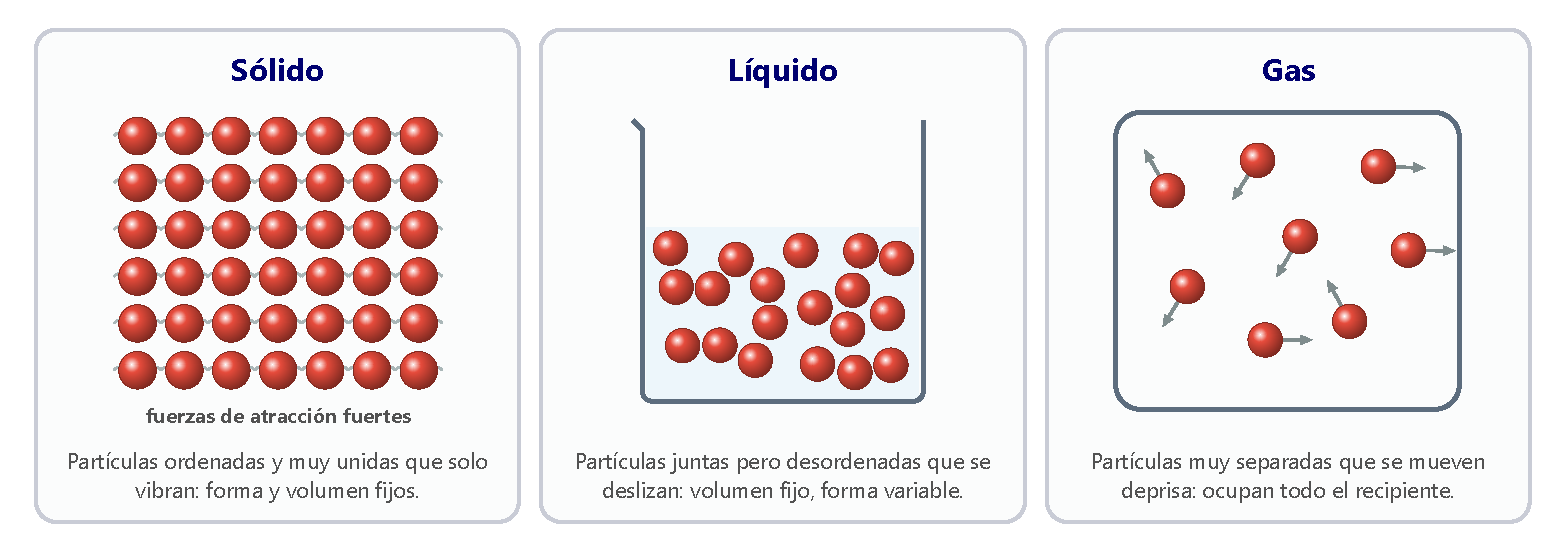
\includegraphics[width=0.85\textwidth]{images/UD1/estados_materia}
    \caption{Modelo de partículas de los tres estados de agregación.}
    \label{fig:ud1-estados}
\end{figure}

\paragraph{Temperatura, presión y volumen.} En el Sistema Internacional la temperatura se mide en \textbf{kelvin}:
\(T(\unit{\kelvin}) = t(\unit{\degreeCelsius}) + 273\). Una variación de \qty{1}{\degreeCelsius} equivale a una de
\qty{1}{\kelvin}. La \textbf{presión} es la fuerza perpendicular por unidad de superficie, \(p = F/S\); su unidad en el SI es el
\textbf{pascal} (\(\qty{1}{\pascal} = \qty{1}{\newton\per\square\metre}\)). La de un gas se debe a los choques de sus partículas
contra las paredes. Con su barómetro de mercurio, \textbf{Torricelli} demostró en 1643 que el aire pesa: al nivel del mar
sostiene una columna de mercurio de \qty{760}{\mm}. El \textbf{volumen} se mide en \unit{\cubic\metre}, aunque se usa mucho
el litro.

\begin{table}[H]
    \centering
    \caption{Equivalencias entre unidades de presión y de volumen}
    \vspace{-5pt}
    \begin{tabular}{@{}ll@{}}
        \toprule
        \textbf{Presión} & \textbf{Volumen} \\
        \midrule
        \(\qty{1}{\atm} = \qty{1.013e5}{\pascal}\) & \(\qty{1}{\cubic\metre} = \qty{1000}{\litre}\) \\[3pt]
        \(\qty{1}{\atm} = \qty{1.013}{\bar} = \qty{1013}{\milli\bar}\) & \(\qty{1}{\cubic\deci\metre} = \qty{1}{\litre}\) \\[3pt]
        \(\qty{1}{\atm} = \qty{760}{\mmHg}\) & \(\qty{1}{\cubic\centi\metre} = \qty{1}{\milli\litre}\) \\
        \bottomrule
    \end{tabular}
    \label{tab:ud1-unidades}
\end{table}

%========================================================================================
\section{Leyes ponderales}\label{sec:ud1-ponderales}
%========================================================================================

Las \textbf{leyes ponderales} son las leyes experimentales que relacionan las \textbf{masas} de las sustancias que intervienen
en una reacción química. Se descubrieron a finales del siglo \textsc{xviii} y comienzos del \textsc{xix}, cuando las balanzas
permitieron pesar con precisión.

\subsection{Ley de conservación de la masa o de Lavoisier}

\textbf{Antoine L. Lavoisier} (1743-1794) quería explicar por qué unas sustancias, como la madera, pierden masa al arder,
mientras que los metales, al calentarlos en el aire, se cubren de una capa de óxido y ganan masa. En su época se aceptaba la
teoría del \textbf{flogisto}: un fluido invisible que las sustancias ganaban o perdían al calentarse.

Lavoisier calentó estaño en un \textbf{recipiente cerrado} con aire. El estaño se transformó en un polvo (un óxido), pero la
masa del recipiente con todo su contenido \textbf{no cambió} (figura~\ref{fig:ud1-lavoisier}). Al abrirlo entraba aire, y la
masa del óxido era mayor que la del estaño inicial: el metal había tomado algo del aire, un componente que él mismo llamó
\textbf{oxígeno}. Este y otros experimentos le llevaron a enunciar:

\begin{definition}[Ley de conservación de la masa]
    En una reacción química, la masa total de las sustancias que intervienen permanece constante: la suma de las masas de los
    \textbf{reactivos} es igual a la suma de las masas de los \textbf{productos}.
\end{definition}

\begin{figure}[H]
    \centering
    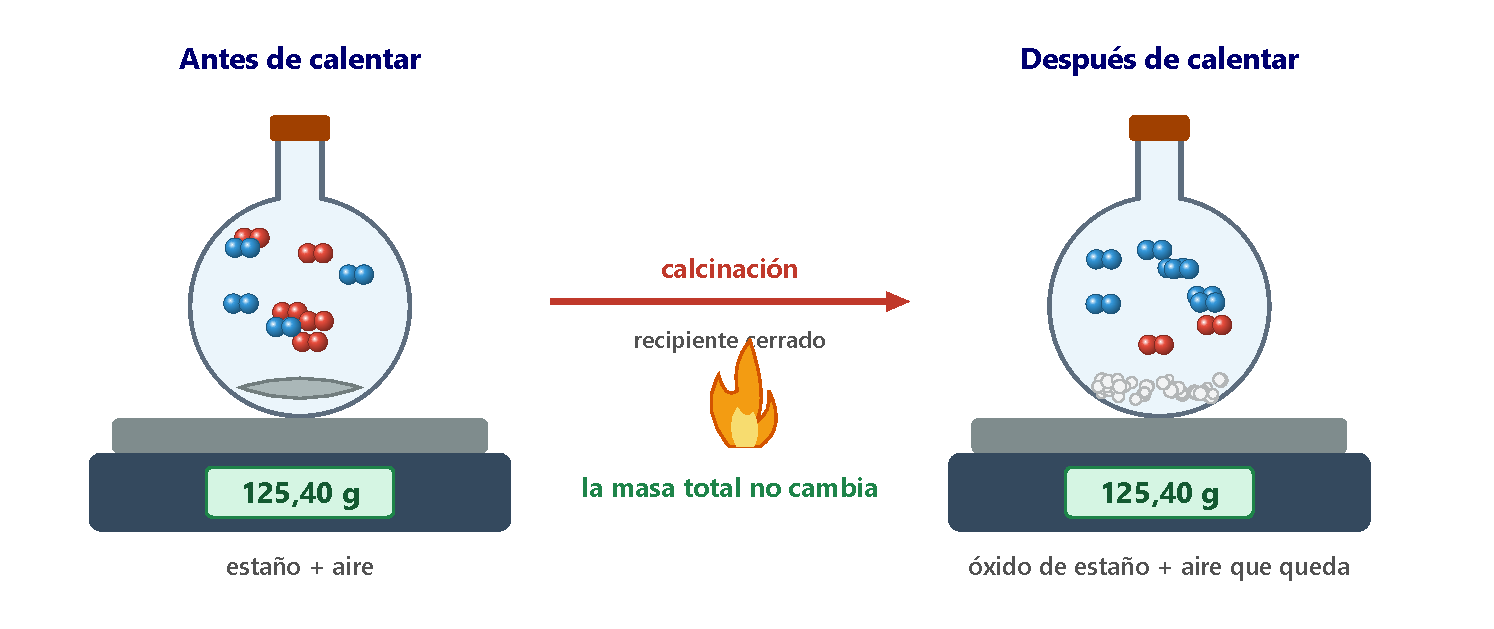
\includegraphics[width=0.85\textwidth]{images/UD1/conservacion_masa}
    \caption{El experimento de Lavoisier: al calcinar estaño en un recipiente cerrado, la masa total no cambia.}
    \label{fig:ud1-lavoisier}
\end{figure}

\begin{remark}
    La ley de Lavoisier no se cumple de forma exacta en las reacciones nucleares, en las que una pequeña parte de la masa se
    transforma en energía según la ecuación de Einstein, \(E = m c^2\). En las reacciones químicas esa variación es tan
    pequeña que no se puede medir.
\end{remark}

\begin{exercise}
    El carbono y el oxígeno se combinan para formar dióxido de carbono. Completa la tabla, sabiendo que en cada experiencia
    reaccionan completamente las masas indicadas.
    \begin{center}
        \begin{tabular}{@{}ccc@{}}
            \toprule
            \textbf{Carbono (g)} & \textbf{Oxígeno (g)} & \textbf{Dióxido de carbono (g)} \\
            \midrule
            12 & 32 & A \\[3pt]
            6 & B & 22 \\[3pt]
            C & 8 & 11 \\
            \bottomrule
        \end{tabular}
    \end{center}
    \begin{solu}
        \textcolor{blue}{Por la ley de Lavoisier, \(m_{\ch{C}} + m_{\ch{O}} = m_{\ch{CO2}}\):}
        \(A = 12 + 32 = \textcolor{red}{\qty{44}{\gram}}\); \(B = 22 - 6 = \textcolor{red}{\qty{16}{\gram}}\);
        \(C = 11 - 8 = \textcolor{red}{\qty{3}{\gram}}\).
    \end{solu}
\end{exercise}

\subsection{Ley de las proporciones definidas o de Proust}

El farmacéutico y químico francés \textbf{Joseph L. Proust} (1754-1826), que trabajó muchos años en España, analizó el
carbonato de cobre(II), \ch{CuCO3}, y comprobó que \textbf{cualquier muestra} contenía 5,3 partes de cobre, 1 de carbono y 4
de oxígeno, tanto si se había preparado en el laboratorio como si se había extraído de un mineral.

\begin{definition}[Ley de las proporciones definidas]
    Cuando dos o más elementos se combinan para formar un determinado compuesto, lo hacen siempre en una
    \textbf{proporción en masa fija}, independientemente del método de obtención o del estado físico del compuesto:
    \[ \frac{m_{\text{elemento A}}}{m_{\text{elemento B}}} = \text{constante} \]
\end{definition}

En el carbonato de cobre(II), la relación entre las masas de cobre y oxígeno es \(5{,}3/4 = \num{1.325}\). Esto permite
calcular la masa de un elemento conociendo la del otro: si una muestra contiene \qty{12}{\gram} de oxígeno, contiene
\(\num{1.325} \cdot 12 = \qty{15.9}{\gram}\) de cobre.

\begin{example}
    \textbf{Combinación del sodio y el cloro.} \qty{46}{\gram} de sodio reaccionan exactamente con \qty{71}{\gram} de cloro para
    dar cloruro de sodio. a) ¿En qué proporción en masa se combinan? b) ¿Cuántos gramos de cloro hacen falta para \qty{30}{\gram}
    de sodio?

    \textbf{Solución.} a) \(\dfrac{m_{\ch{Na}}}{m_{\ch{Cl}}} = \dfrac{46}{71} = \num{0.648}\): \num{0.648} g de sodio por cada
    gramo de cloro. También se puede dar al revés: \(\dfrac{m_{\ch{Cl}}}{m_{\ch{Na}}} = \dfrac{71}{46} = \num{1.54}\) g de cloro
    por cada gramo de sodio.

    b) La proporción se mantiene: \(\dfrac{m_{\ch{Cl}}}{30} = \dfrac{71}{46} \Rightarrow m_{\ch{Cl}} = \dfrac{71 \cdot 30}{46} =
    \qty{46.3}{\gram}\) de cloro.
\end{example}

\begin{exercise}
    \qty{42}{\gram} de hierro reaccionan con \qty{18}{\gram} de oxígeno para formar un óxido. ¿En qué proporción se combinan el
    hierro y el oxígeno?
    \begin{solu}
        \(\dfrac{m_{\ch{Fe}}}{m_{\ch{O}}} = \dfrac{42}{18} = \textcolor{red}{\dfrac{7}{3} = \num{2.33}}\): \textcolor{blue}{7 g de
        hierro por cada 3 g de oxígeno.}
    \end{solu}
\end{exercise}

\begin{exercise}
    El hierro y el azufre forman sulfuro de hierro(II) en una proporción en masa \(7:4\). ¿Cuántos gramos de hierro hacen
    falta para que reaccionen \qty{60}{\gram} de azufre?
    \begin{solu}
        \(\dfrac{m_{\ch{Fe}}}{m_{\ch{S}}} = \dfrac{7}{4} \Rightarrow m_{\ch{Fe}} = \dfrac{7 \cdot 60}{4} =
        \textcolor{red}{\qty{105}{\gram}}\) de hierro.
    \end{solu}
\end{exercise}

\subsection{Ley de las proporciones múltiples o de Dalton}

Algunos químicos de la época, como \textbf{Berthollet} (1748-1822), dudaron de la ley de Proust, porque observaban que dos
elementos podían unirse en \textbf{proporciones distintas} según las condiciones. Al quemar carbón en un lugar bien ventilado,
el gas que se forma tiene 8 partes de oxígeno por cada 3 de carbono; si hay poco oxígeno, tiene 4 partes de oxígeno por cada
3 de carbono.

\textbf{John Dalton} (1766-1844) dio con la explicación: no es un mismo compuesto con proporciones variables, sino \textbf{dos
compuestos diferentes}, el dióxido de carbono, \ch{CO2}, y el monóxido de carbono, \ch{CO}, y cada uno cumple la ley de
Proust. Además, observó que las masas de oxígeno que se combinan con la misma masa de carbono (3 g) guardan una relación muy
sencilla: \(8/4 = 2/1\).

\begin{definition}[Ley de las proporciones múltiples]
    Cuando dos elementos se combinan entre sí para formar más de un compuesto, las masas de un elemento que se combinan con
    una masa fija del otro guardan entre sí una relación de \textbf{números enteros sencillos}.
\end{definition}

\begin{example}
    \textbf{Agua y agua oxigenada.} En el agua, \qty{2}{\gram} de hidrógeno se combinan con \qty{16}{\gram} de oxígeno; en el
    agua oxigenada, \qty{3}{\gram} de hidrógeno se combinan con \qty{48}{\gram} de oxígeno. a) Comprueba que se cumple la ley de
    las proporciones múltiples. b) ¿Cuánto oxígeno se combina con \qty{30}{\gram} de hidrógeno en cada compuesto?

    \textbf{Solución.} a) Calculamos la masa de oxígeno que se combina con \qty{1}{\gram} de hidrógeno en cada compuesto:
    \[ \text{agua: } \frac{16}{2} = \qty{8}{\gram}; \qquad \text{agua oxigenada: } \frac{48}{3} = \qty{16}{\gram}; \qquad
    \frac{8}{16} = \frac{1}{2} \]
    La relación es de números enteros sencillos (1:2): por cada gramo de hidrógeno, el agua oxigenada tiene el doble de
    oxígeno que el agua.

    b) En el agua, \(30 \cdot 8 = \qty{240}{\gram}\) de oxígeno; en el agua oxigenada, el doble: \qty{480}{\gram}.
\end{example}

\begin{exercise}
    En el laboratorio se obtienen dos cloruros de cromo distintos. En el primero, \qty{7.8}{\gram} de cromo se combinan con
    \qty{10.65}{\gram} de cloro; en el segundo, \qty{10.4}{\gram} de cromo se combinan con \qty{21.30}{\gram} de cloro.
    Demuestra que se cumple la ley de las proporciones múltiples.
    \begin{solu}
        \textcolor{blue}{Masa de cloro por gramo de cromo:} primer compuesto \(10{,}65/7{,}8 = \num{1.365}\) g; segundo
        compuesto \(21{,}30/10{,}4 = \num{2.048}\) g.
        \textcolor{blue}{Relación:} \(\dfrac{\num{2.048}}{\num{1.365}} = \num{1.5} = \textcolor{red}{\dfrac{3}{2}}\), \textcolor{red}{números
        enteros sencillos: se cumple la ley de Dalton} (son \ch{CrCl2} y \ch{CrCl3}).
    \end{solu}
\end{exercise}

%========================================================================================
\section{Teoría atómica de Dalton}\label{sec:ud1-dalton}
%========================================================================================

En los siglos \textsc{v} y \textsc{iv} a.\,C. los filósofos griegos se preguntaban si la materia se puede dividir
indefinidamente. El \textbf{atomismo} de \textbf{Leucipo} y \textbf{Demócrito} sostenía que no: que todo está formado por
partículas diminutas e indivisibles, los \emph{átomos}. La \textbf{teoría continuista} de \textbf{Aristóteles}, en cambio,
defendía que la materia se puede dividir sin límite y que todo está formado por cuatro elementos (tierra, agua, aire y fuego).
Fue la idea aceptada durante unos 2000 años.

A comienzos del siglo \textsc{xix}, \textbf{Dalton} se dio cuenta de que las leyes ponderales no encajaban con una materia
continua: si la materia pudiera dividirse sin límite, ¿por qué los elementos se combinan siempre en proporciones fijas? Retomó
la idea de discontinuidad y, en 1808, publicó su \textbf{teoría atómica}:

\begin{definition}[Postulados de la teoría atómica de Dalton]
    \leavevmode % el título de la definición en su propia línea, la lista debajo
    \begin{enumerate}[label=\numberballblue]
        \item Los elementos están formados por partículas extraordinariamente pequeñas e indivisibles, los \textbf{átomos}.
        \item Todos los átomos de un mismo elemento son \textbf{idénticos} (misma masa, mismo tamaño y mismas propiedades); los
        de elementos distintos tienen masa y propiedades diferentes.
        \item Los compuestos se forman por la unión de átomos de elementos distintos en una \textbf{relación de números enteros
        sencillos}, formando «átomos compuestos» (hoy diríamos \textbf{moléculas}).
        \item En una reacción química, los átomos ni se crean ni se destruyen: solo se \textbf{recombinan}.
    \end{enumerate}
\end{definition}

\begin{figure}[H]
    \centering
    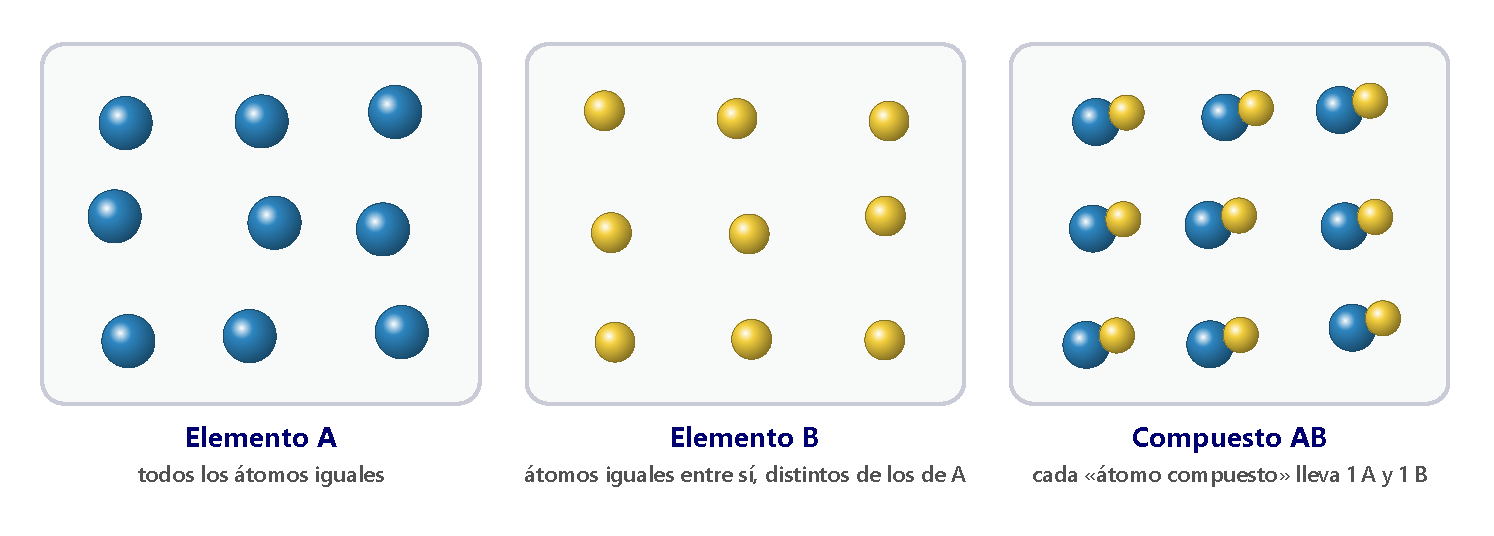
\includegraphics[width=0.85\textwidth]{images/UD1/dalton_teoria}
    \caption{Según Dalton, los átomos de un elemento son iguales entre sí, y un compuesto está formado por «átomos
    compuestos» idénticos.}
    \label{fig:ud1-dalton}
\end{figure}

\begin{remark}
    \textbf{¡Qué curioso!} Además de sus aportaciones a la química, Dalton fue el primero en describir la ceguera a los colores
    que él mismo padecía. Por eso, a esa alteración de la vista la llamamos \textbf{daltonismo}.
\end{remark}

\subsection{La teoría de Dalton explica las leyes ponderales}

\begin{itemize}
    \item \textbf{Conservación de la masa.} Por el postulado 4, en una reacción los átomos solo se recombinan. Antes y después
    hay los mismos átomos, así que la masa total no cambia. Por ejemplo, en \(\ch{2 S + C -> CS2}\), la masa del \ch{CS2} es la
    de dos átomos de azufre más la de uno de carbono.
    \item \textbf{Proporciones definidas.} Por el postulado 3, en un compuesto la relación entre el número de átomos de cada
    elemento es fija. En cualquier muestra de \ch{CO} hay un átomo de C por cada átomo de O, así que la relación entre las masas
    es siempre la de un átomo de C entre la de un átomo de O:
    \(\dfrac{m(\text{4 átomos de C})}{m(\text{4 átomos de O})} = \dfrac{m(\text{átomo de C})}{m(\text{átomo de O})}\).
    \item \textbf{Proporciones múltiples.} Como los átomos no se pueden dividir (postulado 1), una molécula contiene un número
    entero de átomos de cada elemento. En \ch{SO}, \ch{SO2} y \ch{SO3}, las masas de oxígeno unidas a un átomo de azufre son una,
    dos y tres veces la masa de un átomo de oxígeno: relación \(1:2:3\).
\end{itemize}

\begin{figure}[H]
    \centering
    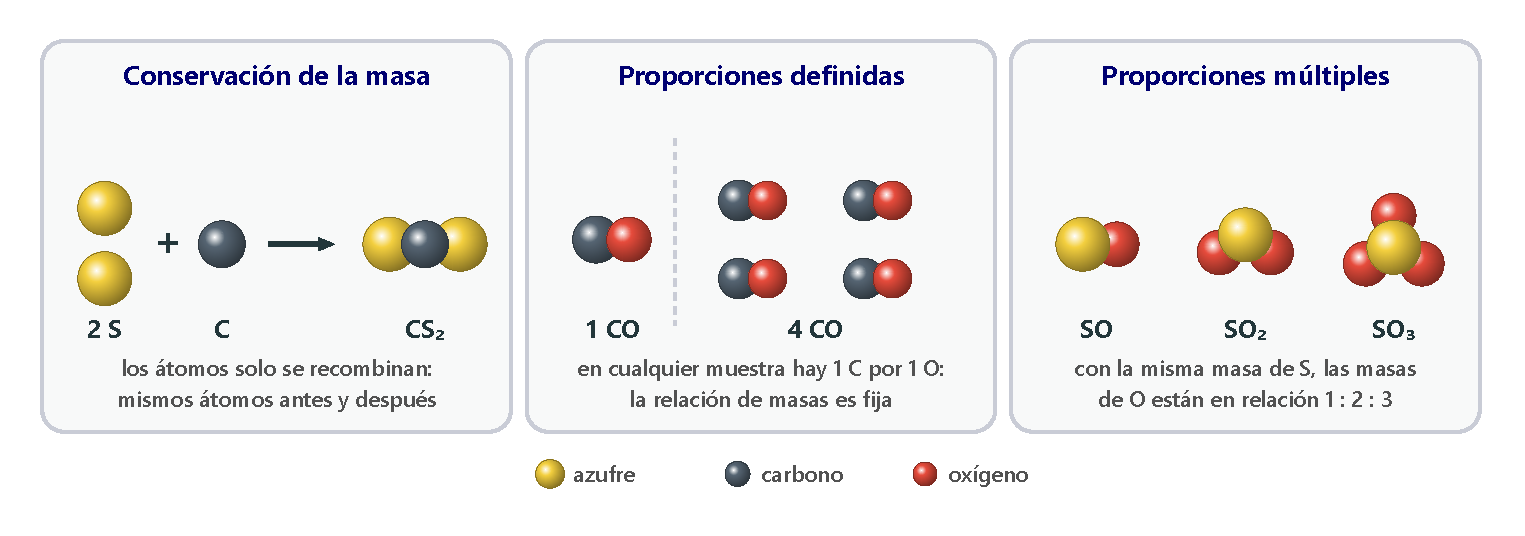
\includegraphics[width=0.9\textwidth]{images/UD1/dalton_leyes}
    \caption{Interpretación de las leyes ponderales con la teoría atómica de Dalton.}
    \label{fig:ud1-dalton-leyes}
\end{figure}

\subsection{Limitaciones de la teoría de Dalton}

La teoría atómica de Dalton fue un gran avance, pero hoy sabemos que tiene errores:
\begin{itemize}
    \item El átomo \textbf{no es indivisible}: está formado por partículas subatómicas (protones, neutrones y electrones).
    \item No todos los átomos de un elemento son idénticos: existen \textbf{isótopos}, átomos del mismo elemento con el mismo
    número de protones pero distinto número de neutrones, y por tanto con distinta masa (el hidrógeno tiene tres: protio,
    deuterio y tritio).
    \item Dalton pensaba que los «átomos compuestos» tenían la composición más sencilla posible. Por eso supuso que el agua
    era \ch{HO} y no \ch{H2O}, y obtuvo masas atómicas erróneas.
\end{itemize}

%========================================================================================
\section{Leyes volumétricas}\label{sec:ud1-volumetricas}
%========================================================================================

Las leyes ponderales se cumplen en cualquier reacción química. Cuando los reactivos y los productos son \textbf{gases}, se
cumplen además unas leyes que relacionan sus \textbf{volúmenes}: la ley de Gay-Lussac y la hipótesis de Avogadro.

\subsection{Ley de los volúmenes de combinación o de Gay-Lussac}

El químico francés \textbf{Joseph L. Gay-Lussac} (1778-1850) midió los volúmenes de gases que reaccionan y se forman,
siempre a la \textbf{misma presión y temperatura}. Encontró, por ejemplo, que 1 L de hidrógeno se combina con 1 L de cloro y
se forman 2 L de cloruro de hidrógeno; que 2 L de hidrógeno reaccionan con 1 L de oxígeno y dan 2 L de vapor de agua; y que
3 L de hidrógeno reaccionan con 1 L de nitrógeno para dar 2 L de amoníaco (figura~\ref{fig:ud1-volumenes}).

\begin{definition}[Ley de los volúmenes de combinación]
    En las reacciones químicas entre gases, los volúmenes de las sustancias que intervienen, medidos en las mismas
    condiciones de presión y temperatura, guardan entre sí una relación de \textbf{números enteros sencillos}.
\end{definition}

Fíjate en que los volúmenes \textbf{no se conservan}: \(3 + 1 \neq 2\). Lo que se conserva es la masa.

\begin{figure}[H]
    \centering
    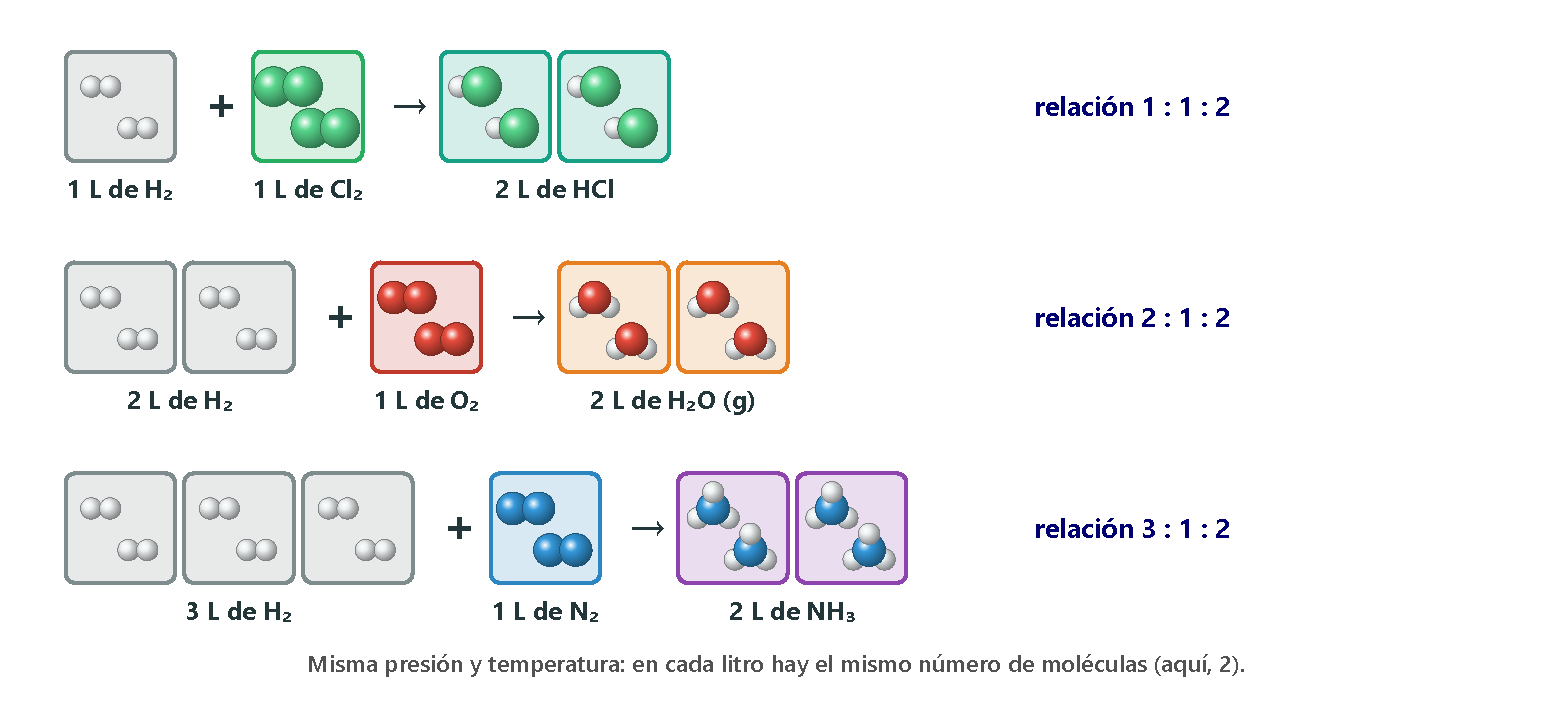
\includegraphics[width=0.9\textwidth]{images/UD1/volumenes_combinacion}
    \caption{Volúmenes de combinación de tres reacciones entre gases, interpretados con la hipótesis de Avogadro.}
    \label{fig:ud1-volumenes}
\end{figure}

\begin{example}
    \textbf{Combustión del monóxido de carbono.} \qty{6}{\litre} de \ch{CO} se combinan con \qty{3}{\litre} de \ch{O2} y se
    obtienen \qty{6}{\litre} de \ch{CO2}, todo medido en las mismas condiciones. a) ¿En qué relación volumétrica reaccionan el
    \ch{CO} y el \ch{O2}? b) ¿Cuántos litros de \ch{CO} hacen falta para \qty{250}{\litre} de oxígeno?

    \textbf{Solución.} a) \(\dfrac{V_{\ch{CO}}}{V_{\ch{O2}}} = \dfrac{6}{3} = 2\): relación \(2:1\).
    b) \(\dfrac{V_{\ch{CO}}}{250} = \dfrac{2}{1} \Rightarrow V_{\ch{CO}} = \qty{500}{\litre}\).
\end{example}

\begin{exercise}
    \(\ch{N2}(g)\) y \(\ch{H2}(g)\) reaccionan para dar amoníaco, \(\ch{NH3}(g)\), en la relación de volúmenes \(1:3:2\).
    Completa la tabla (todos los volúmenes se miden en las mismas condiciones).
    \begin{center}
        \begin{tabular}{@{}ccc@{}}
            \toprule
            \(V(\ch{N2})\) \textbf{(L)} & \(V(\ch{H2})\) \textbf{(L)} & \(V(\ch{NH3})\) \textbf{(L)} \\
            \midrule
            2 & A & B \\[3pt]
            C & 12 & D \\[3pt]
            E & F & 5 \\
            \bottomrule
        \end{tabular}
    \end{center}
    \begin{solu}
        \textcolor{blue}{Con la relación \(1:3:2\):} \(A = 3 \cdot 2 = \textcolor{red}{6}\); \(B = 2 \cdot 2 = \textcolor{red}{4}\);
        \(C = 12/3 = \textcolor{red}{4}\); \(D = 2 \cdot 4 = \textcolor{red}{8}\); \(E = 5/2 = \textcolor{red}{\num{2.5}}\);
        \(F = 3 \cdot \num{2.5} = \textcolor{red}{\num{7.5}}\) (en litros).
    \end{solu}
\end{exercise}

\subsection{La hipótesis de Avogadro}

El italiano \textbf{Amedeo Avogadro} (1776-1856), al estudiar los resultados de Gay-Lussac, pensó que el volumen de un gas
debía estar relacionado con el número de partículas que contiene.

\begin{definition}[Hipótesis de Avogadro]
    Volúmenes iguales de gases diferentes, medidos en las mismas condiciones de presión y temperatura, contienen el
    \textbf{mismo número de partículas}.
\end{definition}

Esta idea parecía chocar con la teoría de Dalton. Si el hidrógeno y el cloro fueran átomos sueltos, de 1 átomo de H y 1 de Cl
saldría 1 «átomo compuesto» de \ch{HCl}, y por tanto de 1 volumen de H y 1 de Cl saldría \textbf{un} volumen de \ch{HCl}. Pero
Gay-Lussac había medido \textbf{dos}. Avogadro resolvió el problema: las partículas de muchos gases no son átomos aislados,
sino agrupaciones de átomos, a las que llamó \textbf{moléculas}. Si el hidrógeno, el cloro, el oxígeno y el nitrógeno son
\textbf{diatómicos} (\ch{H2}, \ch{Cl2}, \ch{O2}, \ch{N2}), todo encaja:
\[ \ch{H2 + Cl2 -> 2 HCl} \qquad \ch{2 H2 + O2 -> 2 H2O} \qquad \ch{3 H2 + N2 -> 2 NH3} \]
Una molécula de \ch{H2} y una de \ch{Cl2} se rompen y se recombinan en dos moléculas de \ch{HCl}; y la misma relación (1:1:2)
aparece entre los volúmenes. Confirmada experimentalmente, la hipótesis de Avogadro pasó a ser una \textbf{ley}.

\begin{example}
    \textbf{Síntesis del amoníaco.} \qty{2}{\litre} de nitrógeno reaccionan con \qty{6}{\litre} de hidrógeno y se obtienen
    \qty{4}{\litre} de amoníaco. Justifica que se cumple la hipótesis de Avogadro.

    \textbf{Solución.} La relación de volúmenes es \(2:6:4 = 1:3:2\). Si en cada litro hay el mismo número de moléculas, por
    cada molécula de \ch{N2} reaccionan 3 de \ch{H2} y se forman 2 de \ch{NH3}: \(\ch{N2 + 3 H2 -> 2 NH3}\). Los átomos cuadran
    (2 de N y 6 de H a cada lado) si cada molécula de amoníaco tiene un átomo de nitrógeno y tres de hidrógeno, que es lo que
    se observa. Por tanto, los datos son coherentes con la hipótesis de Avogadro.
\end{example}

\begin{exercise}
    Al reaccionar \qty{8}{\litre} de hidrógeno con \qty{4}{\litre} de oxígeno se obtienen \qty{8}{\litre} de vapor de agua,
    medidos en las mismas condiciones. Justifica con la hipótesis de Avogadro que la fórmula del agua es \ch{H2O}.
    \begin{solu}
        \textcolor{blue}{Relación de volúmenes \(8:4:8 = 2:1:2\). Si cada litro contiene el mismo número de moléculas, 2 moléculas
        de \ch{H2} y 1 de \ch{O2} dan 2 moléculas de agua: \(\ch{2 H2 + O2 -> 2 H2O}\).} Para que los átomos cuadren (4 de H y 2 de O),
        \textcolor{red}{cada molécula de agua debe tener 2 átomos de H y 1 de O: \ch{H2O}}.
    \end{solu}
\end{exercise}

%========================================================================================
\section{La cantidad de sustancia}\label{sec:ud1-mol}
%========================================================================================

Los átomos son tan pequeños que ninguna balanza puede pesar uno solo. ¿Cómo podemos entonces asignarles una masa? Recuerda
que \textbf{medir es comparar} con una cantidad que tomamos como patrón.

\subsection{Masas atómicas y moleculares}

En el siglo \textsc{xix}, Dalton y otros químicos determinaron la masa de los átomos \textbf{comparándolos entre sí}. Así
averiguaron que el hidrógeno era el más ligero y construyeron una tabla con la masa de cada elemento referida a la del
hidrógeno. Hoy, por acuerdo internacional, el patrón es el átomo de carbono-12 (\(^{12}\)C), al que se asigna una masa de 12
unidades (figura~\ref{fig:ud1-masa-atomica}).

\begin{definition}[Masa atómica relativa]
    La \textbf{masa atómica relativa} de un elemento, \(A_r\), es el número de veces que la masa de uno de sus átomos contiene
    a la doceava parte de la masa de un átomo de \(^{12}\)C:
    \[ A_r = \frac{\text{masa de un átomo del elemento}}{\frac{1}{12}\,(\text{masa de un átomo de } ^{12}\text{C})} \]
\end{definition}

\(A_r\) es un número \textbf{sin unidades}, porque es el cociente de dos masas. En 1960 la IUPAC definió la
\textbf{unidad de masa atómica}, \unit{\uma}, como la doceava parte de la masa de un átomo de \(^{12}\)C:
\[ \qty{1}{\uma} = \qty{1.6605e-27}{\kilogram} \]
La \textbf{masa atómica} de un elemento, \(A\), es la masa de uno de sus átomos expresada en \unit{\uma}. Tiene unidades, pero
coincide numéricamente con \(A_r\): \(A_r(\ch{O}) = 16\) y \(A(\ch{O}) = \qty{16}{\uma}\).

\begin{figure}[H]
    \centering
    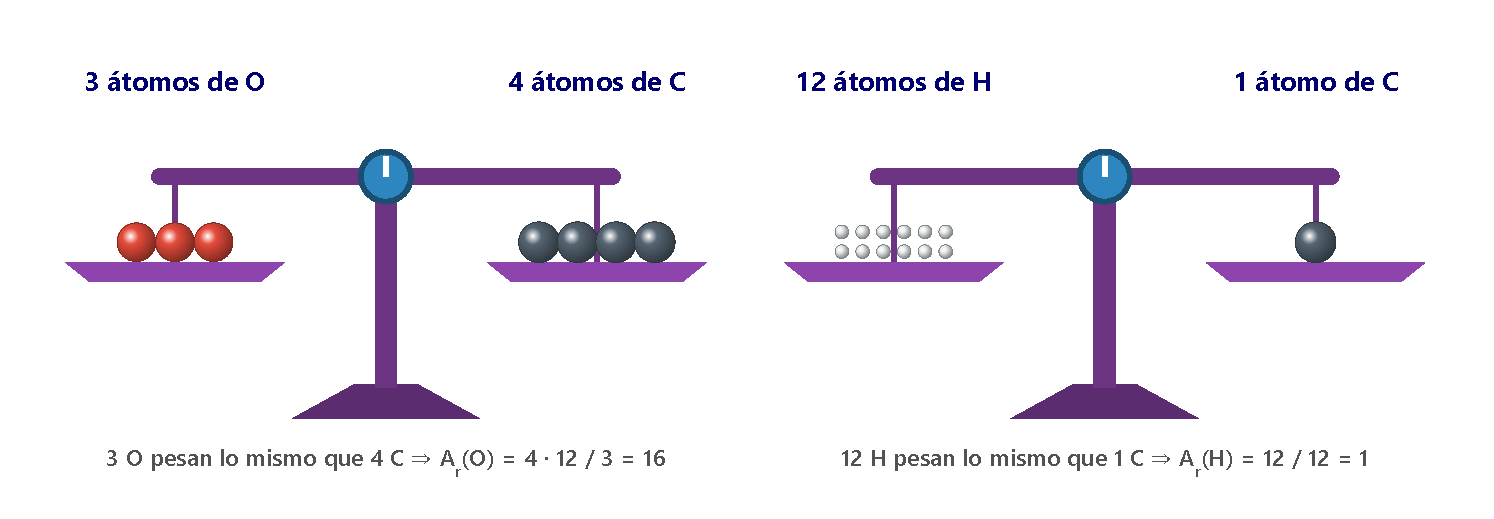
\includegraphics[width=0.85\textwidth]{images/UD1/masa_atomica}
    \caption{Si 3 átomos de oxígeno tienen la misma masa que 4 de carbono (12 cada uno), cada átomo de oxígeno tiene una masa
    relativa de 16.}
    \label{fig:ud1-masa-atomica}
\end{figure}

La \textbf{fórmula} de una sustancia indica los elementos que la forman y la proporción de átomos de cada uno. La masa de una
molécula es la suma de las masas de sus átomos:

\begin{definition}[Masa molecular relativa]
    La \textbf{masa molecular relativa} de un compuesto, \(M_r\), es la suma de las masas atómicas relativas de los átomos que
    forman su molécula. En los compuestos que no forman moléculas (los iónicos, como el \ch{NaCl}, o los cristales covalentes)
    se habla de \textbf{masa fórmula relativa}, calculada con la unidad fórmula.
\end{definition}

Por ejemplo, \(M_r(\ch{H2O}) = 2 \cdot A_r(\ch{H}) + A_r(\ch{O}) = 2 \cdot 1 + 16 = 18\) y
\(M_r(\ch{CO2}) = 12 + 2 \cdot 16 = 44\).

\begin{example}
    \textbf{Masas moleculares.} Calcula la masa molecular de: a) ácido sulfúrico, \ch{H2SO4}; b) etano, \ch{C2H6}; c) nitrógeno,
    \ch{N2}.

    \textbf{Solución.} a) \(M(\ch{H2SO4}) = 2 \cdot 1 + 32 + 4 \cdot 16 = \qty{98}{\uma}\);
    b) \(M(\ch{C2H6}) = 2 \cdot 12 + 6 \cdot 1 = \qty{30}{\uma}\);
    c) \(M(\ch{N2}) = 2 \cdot 14 = \qty{28}{\uma}\).
\end{example}

\subsection{El mol}

Una \textbf{docena} son 12 unidades, sean lápices o huevos. Una docena de lápices y una docena de gomas tienen el mismo número
de objetos, pero distinta masa. Con el \textbf{mol} ocurre lo mismo, pero el número de objetos es enorme, porque los átomos son
diminutos: para tener una cantidad que se pueda pesar con una balanza hacen falta muchísimos.

\begin{definition}[Mol]
    El \textbf{mol} es la unidad de \textbf{cantidad de sustancia} en el Sistema Internacional. Un mol contiene exactamente
    \num{6.022e23} entidades elementales (átomos, moléculas, iones, electrones…). Ese número es el valor de la
    \textbf{constante de Avogadro}:
    \[ N_A = \qty{6.022e23}{\per\mole} \]
\end{definition}

Inicialmente el mol se definió como el número de átomos que hay en \qty{12}{\gram} de \(^{12}\)C; ese número se midió por
varios métodos y resultó ser \num{6.022e23}. Un mol de átomos de carbono contiene \num{6.022e23} átomos de C. Un mol de
moléculas de metano, \ch{CH4}, contiene \num{6.022e23} moléculas, que suman \num{6.022e23} átomos de C y
\(4 \cdot \num{6.022e23} = \num{2.409e24}\) átomos de H.

\begin{remark}
    Un mol de \ch{HCl} y un mol de \ch{H2O} tienen el mismo número de moléculas, pero distinta masa (\qty{36.5}{\gram} y
    \qty{18}{\gram}), igual que una docena de lápices y una docena de gomas.
\end{remark}

\subsection{La masa molar}

\begin{definition}[Masa molar]
    La \textbf{masa molar}, \(M\), de una sustancia es la masa de un mol de sus partículas. Se suele expresar en
    \unit{\gram\per\mole} (en el SI, \unit{\kilogram\per\mole}).
\end{definition}

Como un mol de \(^{12}\)C tiene una masa de \qty{12}{\gram} y cada átomo «vale» 12 unidades, la masa molar de cualquier
sustancia, en \unit{\gram\per\mole}, es \textbf{numéricamente igual} a su masa atómica o molecular relativa. Para el metano:
\(M_r(\ch{CH4}) = 12 + 4 \cdot 1 = 16\), luego \(M(\ch{CH4}) = \qty{16}{\gram\per\mole}\).

\subsection{Cálculos con moles}

La cantidad de sustancia, \(n\), la masa, \(m\), y el número de partículas, \(N\), son directamente proporcionales. Conocida
una de ellas, se calculan las otras con estas fórmulas o con factores de conversión (figura~\ref{fig:ud1-mol}):
\[ n = \frac{m}{M} \qquad\qquad n = \frac{N}{N_A} \]

\begin{figure}[H]
    \centering
    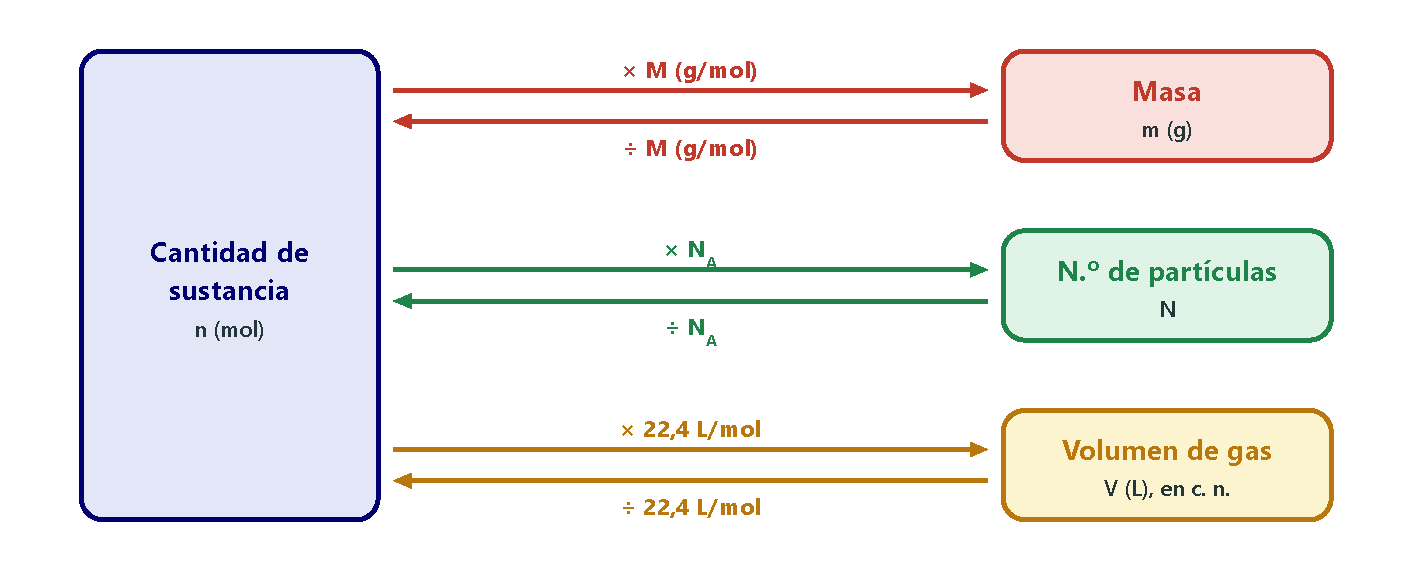
\includegraphics[width=0.75\textwidth]{images/UD1/mol_gas}
    \caption{El mol relaciona la masa, el número de partículas y, en los gases, el volumen (apartado~\ref{sec:ud1-gases-ideales}).}
    \label{fig:ud1-mol}
\end{figure}

\begin{example}
    \textbf{Azúcar en un refresco.} Una lata de refresco lleva el equivalente a 7 terrones de azúcar de \qty{4}{\gram} de
    glucosa, \ch{C6H12O6}, cada uno. Calcula: a) la masa molar de la glucosa; b) los moles de glucosa de la lata; c) los átomos de
    carbono; d) los moles de átomos de oxígeno; e) la masa de hidrógeno; f) la masa de 5 moles de glucosa; g) la masa de glucosa
    que contiene \num{2.4e25} átomos de oxígeno; h) la masa de glucosa que contiene \qty{90}{\gram} de carbono.

    \textbf{Solución.} a) \(M(\ch{C6H12O6}) = 6 \cdot 12 + 12 \cdot 1 + 6 \cdot 16 = \qty{180}{\gram\per\mole}\).

    b) La lata tiene \(7 \cdot 4 = \qty{28}{\gram}\) de glucosa:
    \(\qty{28}{\gram} \cdot \dfrac{\qty{1}{\mole}}{\qty{180}{\gram}} = \qty{0.156}{\mole}\).

    c) \(\qty{0.156}{\mole} \cdot \dfrac{\text{6 mol C}}{\text{1 mol glucosa}} \cdot \dfrac{\num{6.022e23}\text{ átomos}}{\text{1 mol}}
    = \num{5.62e23}\) átomos de C.

    d) \(\qty{0.156}{\mole} \cdot \dfrac{\text{6 mol O}}{\text{1 mol glucosa}} = \qty{0.933}{\mole}\) de átomos de O.

    e) En \qty{180}{\gram} de glucosa hay \qty{12}{\gram} de H: \(28 \cdot \dfrac{12}{180} = \qty{1.87}{\gram}\) de H.

    f) \(\qty{5}{\mole} \cdot \qty{180}{\gram\per\mole} = \qty{900}{\gram}\).

    g) \(\num{2.4e25}\text{ átomos O} \cdot \dfrac{\text{1 mol O}}{\num{6.022e23}\text{ átomos}} \cdot
    \dfrac{\text{1 mol glucosa}}{\text{6 mol O}} \cdot \dfrac{\qty{180}{\gram}}{\text{1 mol glucosa}} = \qty{1196}{\gram}\).

    h) Cada \qty{180}{\gram} de glucosa contienen \(6 \cdot 12 = \qty{72}{\gram}\) de C:
    \(\qty{90}{\gram}\text{ C} \cdot \dfrac{\qty{180}{\gram}\text{ glucosa}}{\qty{72}{\gram}\text{ C}} = \qty{225}{\gram}\) de glucosa.
\end{example}

\begin{exercise}
    En una muestra de \qty{20}{\gram} de sodio, ¿cuántos moles y cuántos átomos de sodio hay?
    \begin{solu}
        \(n = \dfrac{20}{23} = \textcolor{red}{\qty{0.870}{\mole}}\);
        \(N = \num{0.870} \cdot \num{6.022e23} = \textcolor{red}{\num{5.24e23}}\) \textcolor{red}{átomos de Na}.
    \end{solu}
\end{exercise}

\begin{exercise}
    Una olla a presión contiene \num{9.5e23} partículas de aire (78\,\% de \ch{N2} y 21\,\% de \ch{O2}, en número de
    partículas). ¿Cuántas moléculas de cada gas hay?
    \begin{solu}
        \(N(\ch{N2}) = \num{0.78} \cdot \num{9.5e23} = \textcolor{red}{\num{7.41e23}}\);
        \(N(\ch{O2}) = \num{0.21} \cdot \num{9.5e23} = \textcolor{red}{\num{2.00e23}}\) moléculas.
    \end{solu}
\end{exercise}

\begin{exercise}
    Una joya de un metal precioso contiene \num{3.5e23} átomos y tiene una masa de \qty{62.7}{\gram}. a) Calcula la masa molar
    del metal. b) ¿De qué metal se trata?
    \begin{solu}
        a) \(n = \dfrac{\num{3.5e23}}{\num{6.022e23}} = \qty{0.581}{\mole}\);
        \(M = \dfrac{\qty{62.7}{\gram}}{\qty{0.581}{\mole}} = \textcolor{red}{\qty{107.9}{\gram\per\mole}}\).
        b) \textcolor{red}{Plata (Ag)}.
    \end{solu}
\end{exercise}

\begin{exercise}
    El análisis del agua de una laguna indica que hay \num{5e17} átomos de plomo por cada litro. Calcula: a) los átomos de Pb que
    hay en \qty{1}{\cubic\metre} de agua; b) la masa de plomo en \qty{1}{\cubic\metre} de agua.
    \begin{solu}
        a) \(\num{5e17} \cdot 1000 = \textcolor{red}{\num{5e20}}\) átomos.
        b) \(\dfrac{\num{5e20}}{\num{6.022e23}} \cdot \num{207.2} = \textcolor{red}{\qty{0.172}{\gram}}\) de Pb.
    \end{solu}
\end{exercise}

\begin{exercise}
    Una botella de agua contiene \num{4.8e25} átomos de hidrógeno. ¿Qué masa de agua contiene?
    \begin{solu}
        \textcolor{blue}{Cada molécula de \ch{H2O} tiene 2 átomos de H:} \(N(\ch{H2O}) = \num{2.4e25}\) moléculas;
        \(n = \dfrac{\num{2.4e25}}{\num{6.022e23}} = \qty{39.85}{\mole}\); \(m = \num{39.85} \cdot 18 = \qty{717}{\gram} =
        \textcolor{red}{\qty{0.717}{\kilogram}}\).
    \end{solu}
\end{exercise}

%========================================================================================
\section{La fórmula de las sustancias}\label{sec:ud1-formula}
%========================================================================================

La \textbf{fórmula química} indica los elementos que forman una sustancia y la proporción en que están. Hay dos tipos:

\begin{table}[H]
    \centering
    \caption{Fórmula empírica y fórmula molecular}
    \vspace{-5pt}
    \begin{tabular}{@{}L{7cm}L{7cm}@{}}
        \toprule
        \textbf{Fórmula empírica} & \textbf{Fórmula molecular} \\
        \midrule
        Indica qué elementos forman la sustancia y la \textbf{proporción más sencilla}, en números enteros, en que se combinan
        sus átomos. &
        Indica el \textbf{número exacto} de átomos de cada elemento que hay en una molécula. Es un múltiplo entero de la
        empírica. \\[3pt]
        Ácido acético: \ch{CH2O} (por cada átomo de C hay 2 de H y 1 de O). &
        Ácido acético: \ch{C2H4O2} (cada molécula tiene 2 átomos de C, 4 de H y 2 de O). \\
        \bottomrule
    \end{tabular}
    \label{tab:ud1-formulas}
\end{table}

Todos los compuestos tienen fórmula empírica, pero solo los formados por \textbf{moléculas} tienen fórmula molecular. En un
compuesto iónico como el \ch{NaCl} la fórmula solo indica la proporción de iones en el cristal.

\subsection{Composición centesimal}

El hierro se extrae de minerales como la \textbf{hematita}, \ch{Fe2O3}, o la \textbf{siderita}, \ch{FeCO3}. ¿Cuál es más
rentable? El que tenga mayor porcentaje de hierro:
\begin{itemize}
    \item Hematita: \(M(\ch{Fe2O3}) = 2 \cdot \num{55.8} + 3 \cdot 16 = \qty{159.6}{\gram\per\mole}\); en \qty{159.6}{\gram} hay
    \(2 \cdot \num{55.8} = \qty{111.6}{\gram}\) de Fe: \(\%\,\ch{Fe} = \dfrac{\num{111.6}}{\num{159.6}} \cdot 100 = \qty{69.92}{\percent}\).
    \item Siderita: \(M(\ch{FeCO3}) = \num{55.8} + 12 + 3 \cdot 16 = \qty{115.8}{\gram\per\mole}\):
    \(\%\,\ch{Fe} = \dfrac{\num{55.8}}{\num{115.8}} \cdot 100 = \qty{48.19}{\percent}\).
\end{itemize}
La hematita tiene mayor \textbf{riqueza} en hierro.

\begin{definition}[Composición centesimal]
    La \textbf{composición centesimal} de un compuesto es el tanto por ciento en masa de cada elemento, es decir, los gramos de
    cada elemento que hay en \qty{100}{\gram} de compuesto:
    \[ \%\,(\text{elemento}) = \frac{\text{masa del elemento}}{\text{masa del compuesto}} \cdot 100 \]
\end{definition}

Por la ley de Proust, la composición centesimal de un compuesto es \textbf{fija}. Se puede calcular a partir de la masa molar
(como en los ejemplos anteriores) o a partir de cualquier muestra de la que conozcamos la masa total y la de cada elemento.

\subsection{Cálculo de la fórmula empírica}

La fórmula empírica indica la proporción en que se combinan los átomos, y esa misma proporción se da entre los
\textbf{moles} de átomos: en el \ch{Fe2O3}, 3 átomos de O se combinan con 2 de Fe, y 3 moles de O con 2 moles de Fe. Para
obtenerla a partir de la composición centesimal (o de las masas de una muestra):

\begin{enumerate}[label=\numberballblue]
    \item Divide la masa de cada elemento entre su masa atómica: obtienes los \textbf{moles de átomos} de cada uno.
    \item Divide todos los resultados entre el \textbf{más pequeño}: obtienes la relación entre ellos.
    \item Si algún número es decimal (por ejemplo 1,5 o 1,33), \textbf{multiplica} todos por el mismo entero (2, 3…) hasta que
    sean enteros. Esos son los subíndices.
    \item Escribe el símbolo de cada elemento con su subíndice.
\end{enumerate}

\subsection{Cálculo de la fórmula molecular}

La fórmula molecular es un múltiplo de la empírica: fórmula molecular \(= \alpha \cdot{}\)(fórmula empírica).
Para hallar el factor \(\alpha\) hace falta conocer la \textbf{masa molar real} del compuesto (en el apartado~\ref{sec:ud1-gases-ideales}
veremos cómo medirla en los gases):
\[ \alpha = \frac{\text{masa molar real}}{\text{masa molar de la fórmula empírica}} \]
Si la fórmula empírica es \ch{A2B3} y \(\alpha = 2\), la molecular es \ch{A4B6}.

\begin{example}
    \textbf{Fórmula de una sal.} Un compuesto contiene un 17,04\,\% de Na, un 47,41\,\% de S y un 35,55\,\% de O. Su masa molar es
    \qty{270}{\gram\per\mole}. Calcula: a) su fórmula empírica; b) su fórmula molecular.

    \textbf{Solución.} a) Tomamos \qty{100}{\gram} de compuesto y calculamos los moles de átomos de cada elemento; después
    dividimos entre el menor:
    \[ \ch{Na}: \frac{\num{17.04}}{23} = \num{0.741} \rightarrow 1; \qquad
       \ch{S}: \frac{\num{47.41}}{32} = \num{1.482} \rightarrow \frac{\num{1.482}}{\num{0.741}} = 2; \qquad
       \ch{O}: \frac{\num{35.55}}{16} = \num{2.222} \rightarrow \frac{\num{2.222}}{\num{0.741}} = 3 \]
    La fórmula empírica es \ch{NaS2O3}.

    b) \(M(\ch{NaS2O3}) = 23 + 2 \cdot 32 + 3 \cdot 16 = \qty{135}{\gram\per\mole}\); \(\alpha = 270/135 = 2\). La fórmula
    molecular es \ch{Na2S4O6} (tetrationato de sodio).
\end{example}

\begin{exercise}
    Una sal contiene un 40,21\,\% de potasio, un 26,80\,\% de cromo y un 32,99\,\% de oxígeno. Calcula su fórmula empírica.
    \begin{solu}
        \textcolor{blue}{Moles de átomos en \qty{100}{\gram}:} K \(\num{40.21}/39 = \num{1.031}\); Cr \(\num{26.80}/52 = \num{0.515}\);
        O \(\num{32.99}/16 = \num{2.062}\). \textcolor{blue}{Dividiendo entre \num{0.515}:} 2 : 1 : 4.
        \textcolor{red}{Fórmula empírica: \ch{K2CrO4}}.
    \end{solu}
\end{exercise}

\begin{exercise}
    Un compuesto orgánico contiene un 40,0\,\% de C, un 6,7\,\% de H y el resto de oxígeno. a) Calcula su fórmula empírica.
    b) Si \(\alpha = 6\), ¿cuál es su masa molar y su fórmula molecular?
    \begin{solu}
        a) \textcolor{blue}{O: \(100 - 40{,}0 - 6{,}7 = \qty{53.3}{\percent}\).} C \(40{,}0/12 = \num{3.33}\); H \(6{,}7/1 = \num{6.7}\);
        O \(53{,}3/16 = \num{3.33}\) \(\rightarrow\) 1 : 2 : 1. \textcolor{red}{Fórmula empírica: \ch{CH2O}}.
        b) \(M = 6 \cdot 30 = \textcolor{red}{\qty{180}{\gram\per\mole}}\); \textcolor{red}{fórmula molecular \ch{C6H12O6}}.
    \end{solu}
\end{exercise}

%========================================================================================
\section{Las leyes de los gases}\label{sec:ud1-leyes-gases}
%========================================================================================

Las bombonas de oxígeno, los airbags o las ollas a presión son dispositivos diseñados a partir del conocimiento del
comportamiento de los gases. El estado de una cantidad fija de gas queda determinado por tres magnitudes: su
\textbf{presión}, \(p\), su \textbf{volumen}, \(V\), y su \textbf{temperatura}, \(T\). Desde el siglo \textsc{xvii} varios
científicos estudiaron cómo se relacionan, manteniendo \textbf{fija una de ellas} y variando las otras dos
(figura~\ref{fig:ud1-leyes-gases}).

\begin{definition}[Leyes de los gases (para una cantidad fija de gas)]
    \leavevmode % el título de la definición en su propia línea, la lista debajo
    \begin{itemize}
        \item \textbf{Ley de Boyle-Mariotte.} A \textbf{temperatura constante}, el volumen de un gas es inversamente proporcional
        a la presión: \(\;p_1 V_1 = p_2 V_2 = \text{constante}\).
        \item \textbf{Ley de Gay-Lussac.} A \textbf{volumen constante}, la presión de un gas es directamente proporcional a su
        temperatura absoluta: \(\;\dfrac{p_1}{T_1} = \dfrac{p_2}{T_2} = \text{constante}\).
        \item \textbf{Ley de Charles.} A \textbf{presión constante}, el volumen de un gas es directamente proporcional a su
        temperatura absoluta: \(\;\dfrac{V_1}{T_1} = \dfrac{V_2}{T_2} = \text{constante}\).
    \end{itemize}
\end{definition}

\begin{figure}[H]
    \centering
    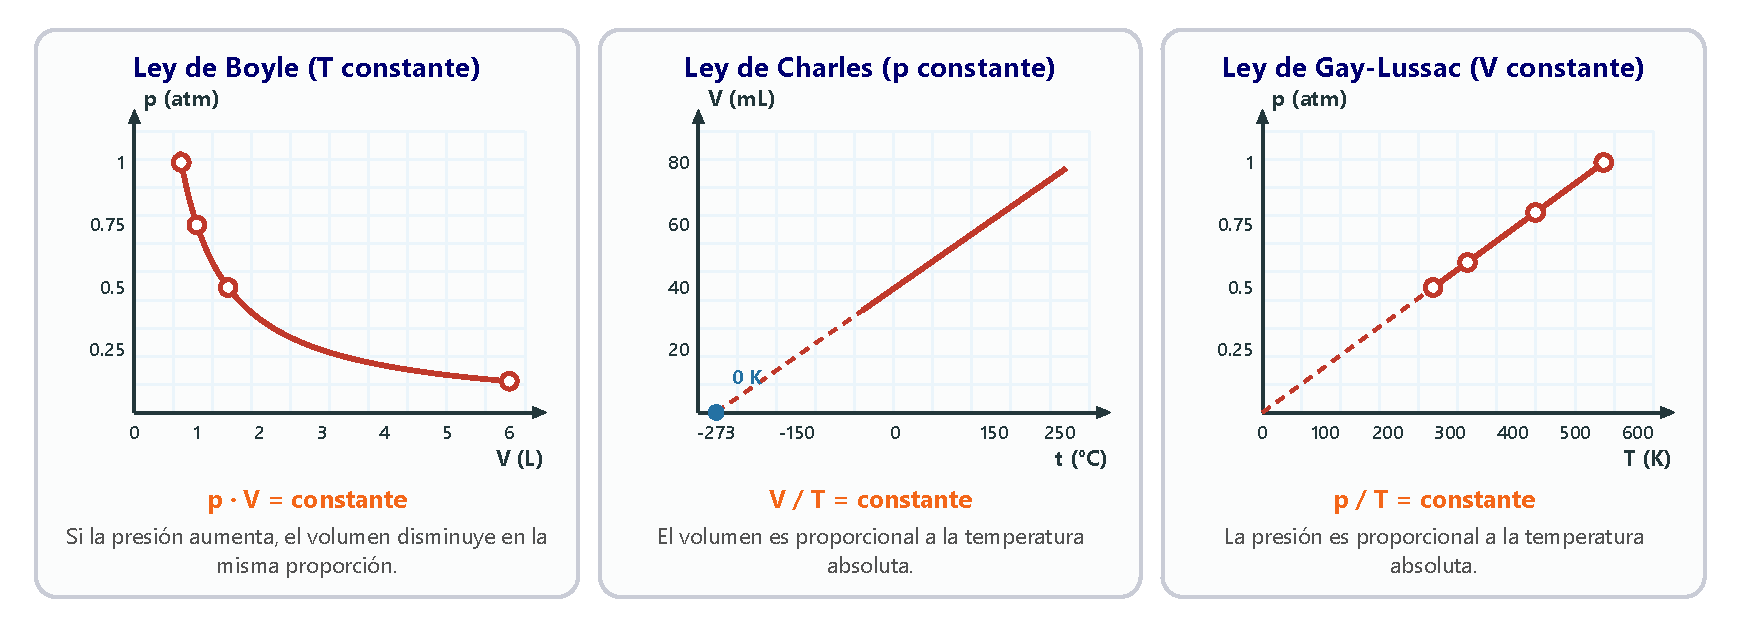
\includegraphics[width=\textwidth]{images/UD1/leyes_gases}
    \caption{Representación gráfica de las tres leyes de los gases.}
    \label{fig:ud1-leyes-gases}
\end{figure}

\begin{remark}
    \textbf{Ten en cuenta.} En las leyes de los gases la presión y el volumen pueden expresarse en cualquier unidad, siempre que
    sea la \textbf{misma} a ambos lados de la igualdad. La temperatura, en cambio, ha de estar siempre en \textbf{kelvin}.
\end{remark}

Si prolongamos hacia la izquierda la recta \(V\)-\(t\) de la ley de Charles, corta al eje de temperaturas en
\qty{-273}{\degreeCelsius}: es el \textbf{cero absoluto}, la temperatura más baja posible, origen de la escala Kelvin.

\begin{exercise}
    Un globo a \qty{850}{\mmHg} ocupa \qty{4}{\cubic\metre}. ¿Qué presión tendrá si reducimos su volumen a la mitad sin cambiar la
    temperatura?
    \begin{solu}
        \textcolor{blue}{Boyle: \(p_2 = p_1 V_1 / V_2 = 850 \cdot 4 / 2\)} \(= \qty{1700}{\mmHg} = \textcolor{red}{\qty{2.24}{\atm}}\).
    \end{solu}
\end{exercise}

\begin{exercise}
    En un recipiente de \qty{20}{\litre} la presión es de \qty{1500}{\milli\bar}. ¿Cuál será su volumen si la presión, a
    temperatura constante, aumenta hasta \qty{3e5}{\pascal}?
    \begin{solu}
        \textcolor{blue}{\(\qty{1500}{\milli\bar} = \qty{1.5e5}{\pascal}\).} \(V_2 = \dfrac{\num{1.5e5} \cdot 20}{\num{3e5}} =
        \textcolor{red}{\qty{10}{\litre}}\).
    \end{solu}
\end{exercise}

\begin{exercise}
    Un gas a \qty{25}{\degreeCelsius} y \qty{500}{\mmHg} se calienta a volumen constante hasta que su presión es de
    \qty{900}{\mmHg}. ¿Cuál es la temperatura final en \unit{\degreeCelsius}?
    \begin{solu}
        \textcolor{blue}{Gay-Lussac:} \(T_2 = T_1 \dfrac{p_2}{p_1} = 298 \cdot \dfrac{900}{500} = \qty{536.4}{\kelvin} =
        \textcolor{red}{\qty{263.4}{\degreeCelsius}}\).
    \end{solu}
\end{exercise}

\begin{exercise}
    La presión del aire en un matraz cerrado es de \qty{480}{\mmHg} a \qty{40}{\degreeCelsius}. ¿Cuál será la presión si se
    calienta hasta \qty{120}{\degreeCelsius}? Supón el volumen constante.
    \begin{solu}
        \(p_2 = p_1 \dfrac{T_2}{T_1} = 480 \cdot \dfrac{393}{313} = \qty{602.7}{\mmHg} = \textcolor{red}{\qty{0.793}{\atm}}\).
    \end{solu}
\end{exercise}

\begin{exercise}
    Un globo ocupa \qty{200}{\cubic\centi\metre} a \qty{10}{\degreeCelsius}. ¿Qué volumen ocuparía a \qty{35}{\degreeCelsius}, a la
    misma presión?
    \begin{solu}
        \textcolor{blue}{Charles:} \(V_2 = V_1 \dfrac{T_2}{T_1} = 200 \cdot \dfrac{308}{283} = \textcolor{red}{\qty{217.7}{\milli\litre}}\).
    \end{solu}
\end{exercise}

\begin{exercise}
    ¿Cómo debe variar la temperatura de un gas para que su volumen se duplique a presión constante?
    \begin{solu}
        \textcolor{blue}{Por la ley de Charles, \(V\) es proporcional a \(T\):} \textcolor{red}{la temperatura absoluta (en kelvin) debe
        duplicarse}. Ojo: no vale duplicar los grados Celsius.
    \end{solu}
\end{exercise}

\subsection{Ley combinada de los gases ideales}

¿Qué ocurre si no se mantiene constante ninguna de las tres magnitudes? Llevamos una cantidad fija de gas desde un estado
inicial \((p_1, T_1, V_1)\) hasta otro final \((p_2, T_2, V_2)\) en dos pasos (figura~\ref{fig:ud1-ley-combinada}):

\begin{enumerate}[label=\numberballblue]
    \item A \textbf{temperatura constante} \(T_1\), cambiamos la presión de \(p_1\) a \(p_2\). El gas pasa a un volumen intermedio
    \(V'\) dado por la ley de Boyle: \(p_1 V_1 = p_2 V' \Rightarrow V' = \dfrac{p_1 V_1}{p_2}\).
    \item A \textbf{presión constante} \(p_2\), cambiamos la temperatura de \(T_1\) a \(T_2\). Por la ley de Charles:
    \(\dfrac{V'}{T_1} = \dfrac{V_2}{T_2} \Rightarrow V' = \dfrac{V_2 T_1}{T_2}\).
\end{enumerate}

Igualando las dos expresiones de \(V'\) y reordenando:

\begin{definition}[Ley combinada de los gases]
    Para una cantidad fija de gas:
    \[ \frac{p_1 V_1}{T_1} = \frac{p_2 V_2}{T_2} \qquad\text{o bien}\qquad \frac{p\,V}{T} = \text{constante} \]
\end{definition}

\begin{figure}[H]
    \centering
    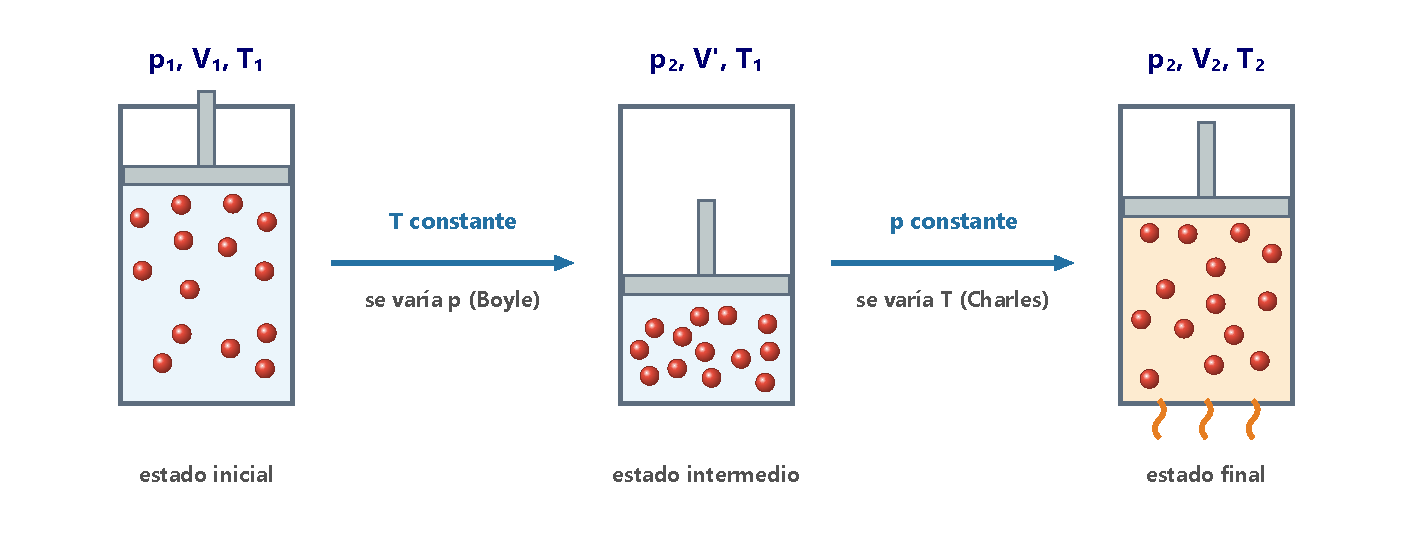
\includegraphics[width=0.8\textwidth]{images/UD1/ley_combinada}
    \caption{Deducción de la ley combinada en dos pasos: primero a \(T\) constante y después a \(p\) constante.}
    \label{fig:ud1-ley-combinada}
\end{figure}

\begin{example}
    \textbf{Calentar un gas.} Un recipiente contiene \qty{4}{\litre} de cloro a \qty{25}{\degreeCelsius} y \qty{750}{\mmHg}. Se
    calienta hasta \qty{50}{\degreeCelsius} y la presión final es de \qty{2}{\atm}. ¿Cuál es el volumen final?

    \textbf{Solución.} Datos: \(p_1 = 750 \cdot \dfrac{1}{760} = \qty{0.987}{\atm}\), \(V_1 = \qty{4}{\litre}\),
    \(T_1 = 25 + 273 = \qty{298}{\kelvin}\); \(p_2 = \qty{2}{\atm}\), \(T_2 = \qty{323}{\kelvin}\).
    \[ \frac{p_1 V_1}{T_1} = \frac{p_2 V_2}{T_2} \Rightarrow V_2 = \frac{p_1 V_1 T_2}{T_1 p_2} =
    \frac{\num{0.987} \cdot 4 \cdot 323}{298 \cdot 2} = \qty{2.14}{\litre} \]
\end{example}

\begin{exercise}
    Un gas ocupa \qty{600}{\milli\litre} a \qty{740}{\mmHg} y \qty{20}{\degreeCelsius}. Si se expande hasta
    \qty{1000}{\milli\litre} y su temperatura sube a \qty{35}{\degreeCelsius}, ¿cuál será su presión?
    \begin{solu}
        \(p_2 = \dfrac{p_1 V_1 T_2}{T_1 V_2} = \dfrac{740 \cdot 600 \cdot 308}{293 \cdot 1000} = \qty{466.7}{\mmHg} =
        \textcolor{red}{\qty{0.614}{\atm}}\).
    \end{solu}
\end{exercise}

%========================================================================================
\section{Teoría cinético-molecular de los gases}\label{sec:ud1-tcm}
%========================================================================================

Las leyes de los gases dicen \emph{cómo} se comportan; la \textbf{teoría cinético-molecular} explica \emph{por qué}. Es un
\textbf{modelo} desarrollado en el siglo \textsc{xix} por \textbf{Joule}, \textbf{Clausius}, \textbf{Maxwell} y
\textbf{Boltzmann}, entre otros.

\begin{definition}[Postulados de la teoría cinético-molecular de los gases]
    \leavevmode % el título de la definición en su propia línea, la lista debajo
    \begin{enumerate}[label=\numberballblue]
        \item Los gases están formados por partículas (átomos o moléculas) de tamaño despreciable frente a las distancias que
        las separan: se pueden considerar \textbf{puntuales}.
        \item Las partículas se mueven continuamente, en línea recta y al \textbf{azar}, chocando entre sí y con las paredes del
        recipiente. Los choques contra las paredes producen la \textbf{presión} del gas.
        \item Los choques son \textbf{elásticos}: no se pierde energía, solo se transfiere de unas partículas a otras.
        \item Las fuerzas de atracción y repulsión entre las partículas son \textbf{despreciables}.
        \item La \textbf{energía cinética media} de las partículas es directamente proporcional a la \textbf{temperatura
        absoluta}: \(\overline{E_c} = k \cdot T\).
    \end{enumerate}
\end{definition}

\subsection{La teoría cinético-molecular explica las leyes de los gases}

\begin{itemize}
    \item \textbf{Boyle-Mariotte.} Si la temperatura no cambia, la velocidad media de las partículas tampoco. Al reducir el
    volumen, tienen menos espacio y chocan con más frecuencia contra las paredes: la presión aumenta.
    \item \textbf{Gay-Lussac.} Si el volumen es fijo y la temperatura sube, las partículas se mueven más deprisa: chocan más a
    menudo y con más fuerza contra las paredes, y la presión aumenta.
    \item \textbf{Charles.} En un recipiente con un émbolo que se mueve libremente, al subir la temperatura los choques más
    frecuentes e intensos empujan el émbolo hacia arriba; el volumen aumenta hasta que la presión interior vuelve a igualar a
    la exterior.
\end{itemize}

\begin{figure}[H]
    \centering
    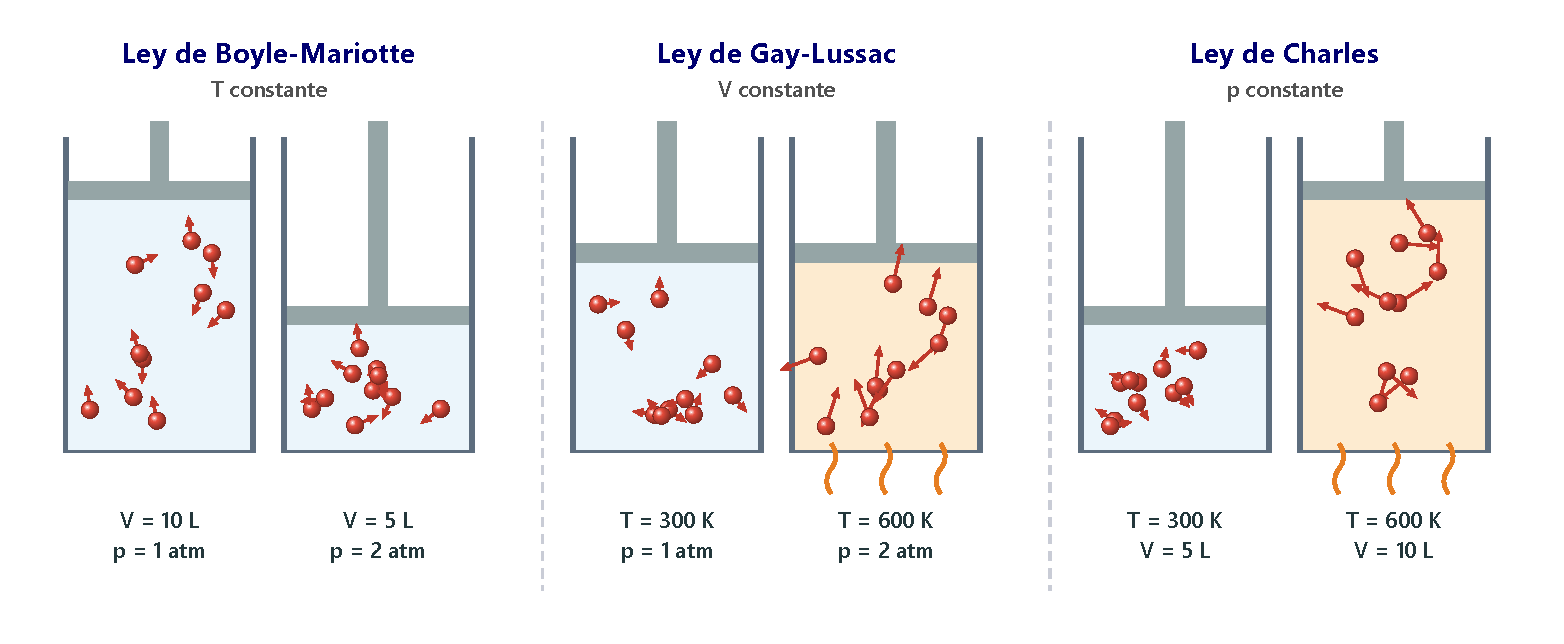
\includegraphics[width=\textwidth]{images/UD1/tcm_leyes}
    \caption{Interpretación cinético-molecular de las leyes de Boyle-Mariotte, Gay-Lussac y Charles. Las flechas indican la
    velocidad de las partículas.}
    \label{fig:ud1-tcm}
\end{figure}

\begin{example}
    \textbf{Temperatura y energía cinética.} ¿Cómo varía la energía cinética de las partículas de un gas si se duplica su
    temperatura absoluta?

    \textbf{Solución.} Según el quinto postulado, \(\overline{E_c} = k\,T\): si \(T\) se duplica, la energía cinética media de
    las partículas también se duplica. Las partículas se mueven más deprisa (su velocidad media aumenta, aunque no al doble,
    porque \(E_c\) depende de \(v^2\)).
\end{example}

%========================================================================================
\section{Ecuación de estado de los gases ideales}\label{sec:ud1-gases-ideales}
%========================================================================================

Un \textbf{gas ideal} es el que cumple exactamente los postulados de la teoría cinético-molecular y, por tanto, las leyes de los
gases. No existe, pero a presiones bajas y temperaturas no muy bajas los gases reales se comportan casi como ideales.

Por la ley de Avogadro, el volumen de un gas a \(p\) y \(T\) dadas es proporcional al número de partículas, es decir, al número
de moles. Por tanto, la constante de la ley combinada, \(p V / T\), es proporcional a \(n\): \(\dfrac{p V}{T} = n R\).

\begin{definition}[Ecuación de estado de los gases ideales]
    \[ p \cdot V = n \cdot R \cdot T \]
    \(R\) es la \textbf{constante de los gases ideales}. Su valor depende de las unidades:
    \(R = \qty{0.082}{\atm\litre\per\mole\per\kelvin}\) (presión en atm y volumen en L) o
    \(R = \qty{8.31}{\pascal\cubic\metre\per\mole\per\kelvin} = \qty{8.31}{\joule\per\mole\per\kelvin}\) (unidades del SI).
\end{definition}

\begin{example}
    \textbf{Valor de \(R\).} Comprueba que \(R\) vale aproximadamente \qty{0.082}{\atm\litre\per\mole\per\kelvin} sabiendo que
    \qty{640}{\gram} de oxígeno, \ch{O2}, a una presión de \qty{4e5}{\pascal}, ocupan \qty{50}{\litre} a \qty{120}{\kelvin}.

    \textbf{Solución.} \(n = \dfrac{640}{32} = \qty{20}{\mole}\); \(p = \dfrac{\num{4e5}}{\num{1.013e5}} = \qty{3.95}{\atm}\).
    \[ R = \frac{p V}{n T} = \frac{\num{3.95} \cdot 50}{20 \cdot 120} = \qty{0.082}{\atm\litre\per\mole\per\kelvin} \]
    El valor coincide con el tabulado: en estas condiciones el oxígeno se comporta como un gas ideal.
\end{example}

\begin{exercise}
    Calcula la presión que ejercen \qty{60}{\gram} de cloro, \ch{Cl2}, en un recipiente de \qty{4}{\cubic\deci\metre} a
    \qty{25}{\degreeCelsius}.
    \begin{solu}
        \(n = 60/71 = \qty{0.845}{\mole}\); \(p = \dfrac{n R T}{V} = \dfrac{\num{0.845} \cdot \num{0.082} \cdot 298}{4} =
        \textcolor{red}{\qty{5.16}{\atm}}\).
    \end{solu}
\end{exercise}

\begin{exercise}
    ¿Qué volumen ocupan \qty{2.5}{\mole} de un gas en condiciones normales (\qty{1}{\atm} y \qty{273}{\kelvin})?
    \begin{solu}
        \(V = \dfrac{n R T}{p} = \num{2.5} \cdot \num{0.082} \cdot 273 = \textcolor{red}{\qty{56}{\litre}}\) \textcolor{blue}{(\(\num{2.5} \cdot \num{22.4}\)).}
    \end{solu}
\end{exercise}

\begin{exercise}
    ¿A qué temperatura deben estar \qty{40}{\gram} de nitrógeno, \ch{N2}, en un recipiente de \qty{400}{\cubic\centi\metre} para
    que su presión sea de \qty{4e6}{\pascal}?
    \begin{solu}
        \(n = 40/28 = \qty{1.43}{\mole}\); \(p = \num{4e6}/\num{1.013e5} = \qty{39.5}{\atm}\);
        \(T = \dfrac{p V}{n R} = \dfrac{\num{39.5} \cdot \num{0.4}}{\num{1.43} \cdot \num{0.082}} = \textcolor{red}{\qty{135}{\kelvin}}\).
    \end{solu}
\end{exercise}

\begin{exercise}
    ¿Qué masa de dióxido de carbono hay en un depósito de \qty{250}{\cubic\metre} en condiciones estándar
    (\qty{1e5}{\pascal} y \qty{273}{\kelvin})?
    \begin{solu}
        \textcolor{blue}{En el SI:} \(n = \dfrac{p V}{R T} = \dfrac{\num{1e5} \cdot 250}{\num{8.31} \cdot 273} = \qty{11020}{\mole}\);
        \(m = \num{11020} \cdot 44 = \qty{4.85e5}{\gram} = \textcolor{red}{\qty{485}{\kilogram}}\).
    \end{solu}
\end{exercise}

\subsection{Volumen molar}

Según la ley de Avogadro, el volumen de un gas no depende de su naturaleza, sino del número de partículas. Se llama
\textbf{volumen molar} al volumen que ocupa un mol de cualquier gas en unas condiciones determinadas. Suelen usarse dos
referencias:
\begin{itemize}
    \item \textbf{Condiciones normales} (c.\,n.): \(p = \qty{1}{\atm}\) y \(T = \qty{273}{\kelvin}\):
    \(V_m = \dfrac{1 \cdot \num{0.082} \cdot 273}{1} = \qty{22.4}{\litre\per\mole}\).
    \item \textbf{Condiciones estándar} de la IUPAC: \(p = \qty{1e5}{\pascal}\) y \(T = \qty{273}{\kelvin}\):
    \(V_m = \qty{22.7}{\litre\per\mole}\).
\end{itemize}

\begin{example}
    \textbf{Volumen de un gas.} Calcula el volumen que ocupan \qty{210}{\gram} de nitrógeno, \ch{N2}, en condiciones estándar.

    \textbf{Solución.} \(\qty{210}{\gram} \cdot \dfrac{\qty{1}{\mole}}{\qty{28}{\gram}} = \qty{7.5}{\mole}\);
    \(\qty{7.5}{\mole} \cdot \dfrac{\qty{22.7}{\litre}}{\qty{1}{\mole}} = \qty{170}{\litre}\).
\end{example}

\subsection{Densidad de un gas}

La densidad de un líquido o de un sólido apenas cambia con las condiciones, pero la de un gas varía mucho con la presión y la
temperatura. Sustituyendo \(n = m/M\) en la ecuación de los gases:
\[ p V = \frac{m}{M} R T \;\Rightarrow\; p = \frac{m}{V} \cdot \frac{R T}{M} = d \cdot \frac{R T}{M} \;\Rightarrow\;
\boxed{d = \frac{p \cdot M}{R \cdot T}} \]
A la misma presión y temperatura, es más denso el gas de \textbf{mayor masa molar}.

\subsection{Masa molar de un gas}

Si no conocemos la fórmula de una sustancia gaseosa, podemos determinar su masa molar en el laboratorio midiendo el volumen
que ocupa una masa conocida a una presión y una temperatura dadas:
\[ p V = \frac{m}{M} R T \;\Rightarrow\; M = \frac{m \cdot R \cdot T}{p \cdot V} \]
Con la masa molar y la fórmula empírica se obtiene la fórmula molecular (apartado~\ref{sec:ud1-formula}).

\begin{example}
    \textbf{Masa molar de un gas.} \qty{45}{\milli\gram} de un gas ocupan \qty{6}{\cubic\centi\metre} en condiciones normales.
    Calcula su masa molar.

    \textbf{Solución.} Pasamos a las unidades de \(R\): \(m = \qty{0.045}{\gram}\), \(V = \qty{0.006}{\litre}\).
    \[ M = \frac{m R T}{p V} = \frac{\num{0.045} \cdot \num{0.082} \cdot 273}{1 \cdot \num{0.006}} = \qty{168}{\gram\per\mole} \]
\end{example}

\subsection{Gases reales}

En condiciones de \textbf{baja presión} y \textbf{alta temperatura}, lejos de los cambios de estado, las partículas están muy
separadas y los gases se comportan casi como ideales. A presiones altas o temperaturas bajas ya no se puede despreciar el
tamaño de las partículas ni las fuerzas entre ellas. En 1873, \textbf{J. D. van der Waals} propuso una ecuación que corrige la
del gas ideal:

\begin{definition}[Ecuación de van der Waals]
    \[ \left(p + \frac{a\,n^2}{V^2}\right)\left(V - n\,b\right) = n R T \]
    La constante \(a\) tiene en cuenta las \textbf{fuerzas de atracción} entre partículas, que reducen la presión; la constante
    \(b\), el \textbf{volumen propio} de las partículas, que reduce el volumen disponible. Ambas son propias de cada gas.
\end{definition}

\begin{remark}
    Si el nitrógeno se comportara como un gas ideal, sus moléculas no se atraerían y nunca se podría licuar. El nitrógeno
    líquido, a \qty{-196}{\degreeCelsius}, se usa en medicina, en la conservación de muestras biológicas y hasta en cocina.
\end{remark}

\begin{example}
    \textbf{Gas real.} Calcula la presión que ejercen \qty{150}{\mole} de aire en un recipiente de \qty{12}{\litre} a
    \qty{30}{\degreeCelsius} con la ecuación de van der Waals (\(a = \qty{1.33}{\atm\litre\squared\per\mole\squared}\),
    \(b = \qty{0.0366}{\litre\per\mole}\)). Compárala con la de un gas ideal.

    \textbf{Solución.} Despejamos la presión:
    \[ p = \frac{n R T}{V - n b} - a \left(\frac{n}{V}\right)^2 = \frac{150 \cdot \num{0.082} \cdot 303}{12 - 150 \cdot \num{0.0366}}
    - \num{1.33} \left(\frac{150}{12}\right)^2 = \num{572.5} - \num{207.8} = \qty{365}{\atm} \]
    Como gas ideal: \(p = \dfrac{150 \cdot \num{0.082} \cdot 303}{12} = \qty{311}{\atm}\). A presiones tan altas la diferencia es
    importante.
\end{example}

\begin{exercise}
    Una sustancia contiene un 24,27\,\% de C, un 4,07\,\% de H y el resto de cloro. \qty{4.00}{\gram} de su vapor ocupan
    \qty{1.24}{\litre} a \qty{100}{\degreeCelsius} y \qty{1}{\atm}. Determina su fórmula molecular.
    \begin{solu}
        \textcolor{blue}{Cl: \qty{71.66}{\percent}.} C \(\num{24.27}/12 = \num{2.02}\); H \(\num{4.07}/1 = \num{4.07}\);
        Cl \(\num{71.66}/\num{35.5} = \num{2.02}\) \(\rightarrow\) 1 : 2 : 1; empírica \ch{CH2Cl}, \(M = \qty{49.5}{\gram\per\mole}\).
        \textcolor{blue}{Masa molar:} \(M = \dfrac{m R T}{p V} = \dfrac{4 \cdot \num{0.082} \cdot 373}{1 \cdot \num{1.24}} = \qty{98.7}{\gram\per\mole}\);
        \(\alpha = \num{98.7}/\num{49.5} = 2\). \textcolor{red}{Fórmula molecular: \ch{C2H4Cl2}}.
    \end{solu}
\end{exercise}

\begin{exercise}
    Calcula la presión ejercida por \qty{4}{\mole} de metanol gaseoso, \ch{CH3OH}, que ocupan \qty{5}{\litre} a \qty{450}{\kelvin}:
    a) suponiendo que es un gas ideal; b) con la ecuación de van der Waals
    (\(a = \qty{9.23}{\atm\litre\squared\per\mole\squared}\), \(b = \qty{0.0651}{\litre\per\mole}\)).
    \begin{solu}
        a) \(p = \dfrac{4 \cdot \num{0.082} \cdot 450}{5} = \textcolor{red}{\qty{29.5}{\atm}}\).
        b) \(p = \dfrac{4 \cdot \num{0.082} \cdot 450}{5 - 4 \cdot \num{0.0651}} - \num{9.23} \left(\dfrac{4}{5}\right)^2 = \num{31.14} - \num{5.91}
        = \textcolor{red}{\qty{25.2}{\atm}}\).
    \end{solu}
\end{exercise}

%========================================================================================
\section{Mezclas de gases}\label{sec:ud1-mezclas}
%========================================================================================

El \textbf{gas natural} que llega a muchas casas es una mezcla: sobre todo metano, con algo de etano, propano, butano,
nitrógeno y dióxido de carbono. El aire también es una mezcla de gases. ¿Cómo se comporta una mezcla?

Se llama \textbf{presión parcial} de un componente, \(p_i\), a la presión que ejercería si estuviera \textbf{él solo} en el
recipiente que ocupa la mezcla, a la misma temperatura. Dalton estudió las mezclas gaseosas y enunció:

\begin{definition}[Ley de Dalton de las presiones parciales]
    La presión total de una mezcla de gases que no reaccionan entre sí es igual a la suma de las presiones parciales de sus
    componentes:
    \[ p_T = p_1 + p_2 + p_3 + \dots = \sum p_i \]
\end{definition}

Cada gas se comporta como si estuviera solo (figura~\ref{fig:ud1-dalton-presiones}). Si en un recipiente de volumen \(V\) y
temperatura \(T\) hay \(n_1\) moles de un gas y \(n_2\) de otro, en total \(n_T = n_1 + n_2\):
\[ p_T = \frac{n_T R T}{V} = \frac{(n_1 + n_2) R T}{V} = \frac{n_1 R T}{V} + \frac{n_2 R T}{V} = p_1 + p_2 \]
Dividiendo la presión parcial de un componente entre la total:
\[ \frac{p_i}{p_T} = \frac{n_i R T / V}{n_T R T / V} = \frac{n_i}{n_T} = \chi_i \]
\(\chi_i\) es la \textbf{fracción molar} del componente: la fracción de las partículas de la mezcla que son de ese gas. Es un
número entre 0 y 1, y la suma de las fracciones molares de todos los componentes vale 1.

\begin{definition}[Presión parcial y fracción molar]
    La presión parcial de un componente de una mezcla de gases es igual a su fracción molar por la presión total:
    \[ p_i = \chi_i \cdot p_T \]
\end{definition}

\begin{figure}[H]
    \centering
    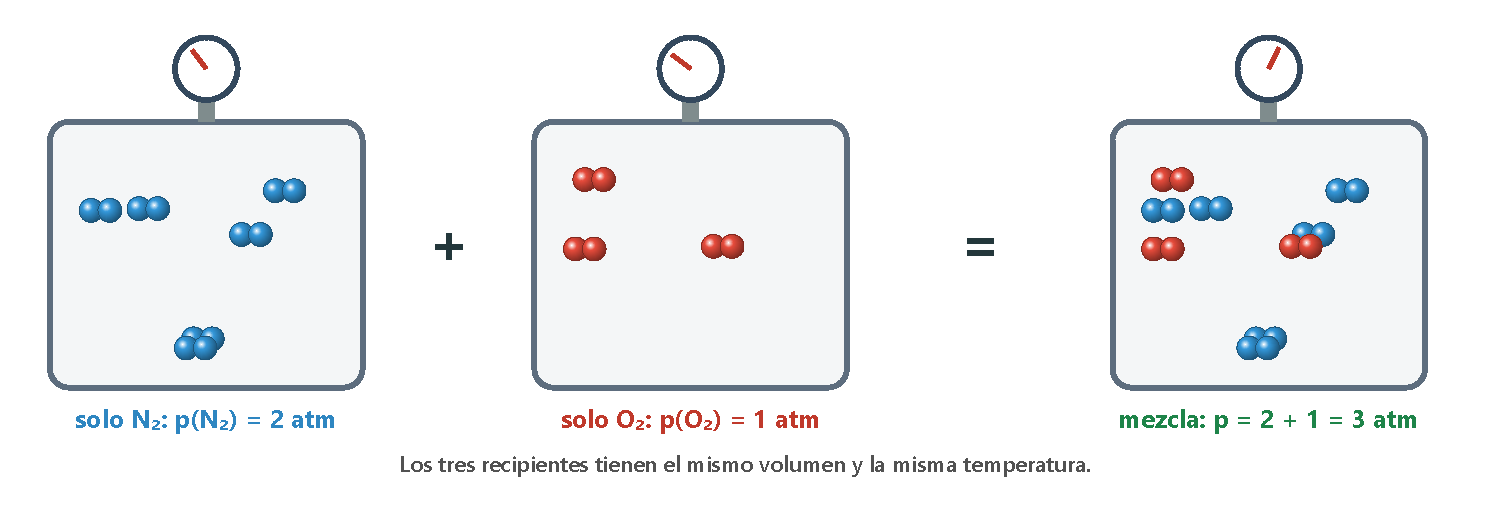
\includegraphics[width=0.85\textwidth]{images/UD1/presiones_parciales}
    \caption{Ley de Dalton: la presión de la mezcla es la suma de las presiones que ejercería cada gas solo.}
    \label{fig:ud1-dalton-presiones}
\end{figure}

\begin{example}
    \textbf{Globo aerostático.} Un globo contiene una mezcla de \qty{70}{\gram} de nitrógeno, \ch{N2}, \qty{32}{\gram} de oxígeno,
    \ch{O2}, y \qty{44}{\gram} de propano, \ch{C3H8}. La presión total es de \qty{4}{\atm}. Calcula la presión parcial de cada
    gas.

    \textbf{Solución.} Moles de cada componente:
    \(n_{\ch{N2}} = \dfrac{70}{28} = \qty{2.5}{\mole}\); \(n_{\ch{O2}} = \dfrac{32}{32} = \qty{1}{\mole}\);
    \(n_{\ch{C3H8}} = \dfrac{44}{44} = \qty{1}{\mole}\); \(n_T = \qty{4.5}{\mole}\).
    \[ p_{\ch{N2}} = \frac{\num{2.5}}{\num{4.5}} \cdot 4 = \qty{2.22}{\atm}; \qquad
       p_{\ch{O2}} = \frac{1}{\num{4.5}} \cdot 4 = \qty{0.89}{\atm}; \qquad
       p_{\ch{C3H8}} = \frac{1}{\num{4.5}} \cdot 4 = \qty{0.89}{\atm} \]
    La suma de las presiones parciales es la presión total: \(\num{2.22} + \num{0.89} + \num{0.89} = \qty{4}{\atm}\).
\end{example}

\begin{exercise}
    Se introducen \qty{120}{\gram} de \ch{CO2} y \qty{140}{\gram} de \ch{CO} en un recipiente de \qty{25}{\litre} a
    \qty{15}{\degreeCelsius}. Calcula: a) la presión total; b) la presión parcial de cada gas.
    \begin{solu}
        a) \(n_{\ch{CO2}} = 120/44 = \qty{2.73}{\mole}\); \(n_{\ch{CO}} = 140/28 = \qty{5}{\mole}\); \(n_T = \qty{7.73}{\mole}\).
        \(p_T = \dfrac{\num{7.73} \cdot \num{0.082} \cdot 288}{25} = \textcolor{red}{\qty{7.30}{\atm}}\).
        b) \(p_{\ch{CO2}} = \dfrac{\num{2.73}}{\num{7.73}} \cdot \num{7.30} = \textcolor{red}{\qty{2.58}{\atm}}\);
        \(p_{\ch{CO}} = \dfrac{5}{\num{7.73}} \cdot \num{7.30} = \textcolor{red}{\qty{4.72}{\atm}}\).
    \end{solu}
\end{exercise}

\begin{exercise}
    Un globo de \qty{6}{\litre} a \qty{25}{\degreeCelsius} contiene helio y hidrógeno con presiones parciales
    \(p(\ch{He}) = \qty{0.6}{\atm}\) y \(p(\ch{H2}) = \qty{0.8}{\atm}\). Calcula: a) la presión total; b) los moles totales;
    c) los moles de cada gas.
    \begin{solu}
        a) \(p_T = \num{0.6} + \num{0.8} = \textcolor{red}{\qty{1.4}{\atm}}\).
        b) \(n_T = \dfrac{\num{1.4} \cdot 6}{\num{0.082} \cdot 298} = \textcolor{red}{\qty{0.344}{\mole}}\).
        c) \(n_{\ch{He}} = \dfrac{\num{0.6}}{\num{1.4}} \cdot \num{0.344} = \textcolor{red}{\qty{0.147}{\mole}}\);
        \(n_{\ch{H2}} = \textcolor{red}{\qty{0.196}{\mole}}\).
    \end{solu}
\end{exercise}

\begin{exercise}
    El aire tiene, en volumen, un 21\,\% de \ch{O2}, un 78\,\% de \ch{N2} y un 1\,\% de argón. En lo alto de una montaña la
    presión atmosférica es de \qty{0.95}{\atm}. ¿Qué presión ejerce cada gas?
    \begin{solu}
        \textcolor{blue}{En los gases, el porcentaje en volumen coincide con la fracción molar.}
        \(p_{\ch{O2}} = \num{0.21} \cdot \num{0.95} = \textcolor{red}{\qty{0.200}{\atm}}\);
        \(p_{\ch{N2}} = \num{0.78} \cdot \num{0.95} = \textcolor{red}{\qty{0.741}{\atm}}\);
        \(p_{\ch{Ar}} = \num{0.01} \cdot \num{0.95} = \textcolor{red}{\qty{0.0095}{\atm}}\).
    \end{solu}
\end{exercise}

\begin{exercise}
    En una botella de \qty{3}{\litre} a \qty{20}{\degreeCelsius}, la presión debida al oxígeno es de \qty{1200}{\mmHg} y la del
    nitrógeno, de \qty{2800}{\mmHg}. Calcula la masa de cada gas.
    \begin{solu}
        \(p_{\ch{O2}} = 1200/760 = \qty{1.58}{\atm}\): \(n = \dfrac{\num{1.58} \cdot 3}{\num{0.082} \cdot 293} = \qty{0.197}{\mole}\),
        \(m = \textcolor{red}{\qty{6.3}{\gram}}\) de \ch{O2}.
        \(p_{\ch{N2}} = 2800/760 = \qty{3.68}{\atm}\): \(n = \qty{0.460}{\mole}\), \(m = \textcolor{red}{\qty{12.9}{\gram}}\) de \ch{N2}.
    \end{solu}
\end{exercise}

%========================================================================================
\section{Química en la vida: ¿cómo funciona una olla a presión?}\label{sec:ud1-olla}
%========================================================================================

En una olla corriente, el agua no puede pasar de \qty{100}{\degreeCelsius}: a esa temperatura hierve y el calor que le
damos se emplea en evaporarla. En una \textbf{olla a presión} (u olla exprés) la tapa cierra herméticamente. Al calentar, el
vapor no puede escapar y la presión dentro aumenta, igual que en la ley de Gay-Lussac. Y cuanto mayor es la presión, mayor es
la temperatura a la que hierve el agua (figura~\ref{fig:ud1-olla}): con unos \qty{2}{\bar}, el agua hierve a unos
\qty{120}{\degreeCelsius}, y los alimentos se cuecen hasta un 70\,\% más rápido.

\begin{figure}[H]
    \centering
    \begin{tikzpicture}
        \begin{axis}[grafica, width=0.6\linewidth, height=5.2cm,
            xlabel={\(t\) (\unit{\degreeCelsius})}, ylabel={\(p\) (\unit{\atm})},
            xmin=0, xmax=135, ymin=0, ymax=3.2, xtick={0,20,...,140}]
            \addplot[thick, red!75!black, domain=0:132] {10^(8.07131 - 1730.63/(233.426 + x))/760};
            \addplot[dashed, gray] coordinates {(0,1) (100,1) (100,0)};
            \addplot[dashed, gray] coordinates {(0,1.96) (120,1.96) (120,0)};
            \node[font=\scriptsize, anchor=south east] at (axis cs:98,1) {olla abierta};
            \node[font=\scriptsize, anchor=south east] at (axis cs:118,1.96) {olla a presión};
        \end{axis}
    \end{tikzpicture}
    \caption{Presión a la que hierve el agua en función de la temperatura (presión de vapor del agua).}
    \label{fig:ud1-olla}
\end{figure}

Cuando se alcanza la presión máxima, una \textbf{válvula} (con un muelle o un contrapeso) se abre y deja salir vapor, de modo
que la presión ya no sube más. Desde ese momento no sirve de nada mantener el fuego fuerte: basta con un fuego bajo que
mantenga la presión, y así se ahorra energía. El silbido característico de algunas ollas lo produce el vapor al salir por el
pequeño orificio de la válvula.

\begin{exercise}
    a) ¿Qué ley de los gases explica que la presión aumente al calentar la olla cerrada? b) ¿Por qué se cocinan antes los
    alimentos en una olla a presión? c) ¿Por qué no conviene abrir la olla nada más apagar el fuego?
    \begin{solu}
        a) \textcolor{red}{La ley de Gay-Lussac}: a volumen constante, la presión es proporcional a la temperatura absoluta (además, al
        evaporarse agua aumenta la cantidad de gas). b) \textcolor{red}{Porque a mayor presión el agua hierve a mayor temperatura}
        (unos \qty{120}{\degreeCelsius} a \qty{2}{\bar}), y las reacciones de la cocción son más rápidas. c) \textcolor{red}{Porque dentro
        la presión sigue siendo alta}: al abrirla, el vapor y el agua muy caliente saldrían con violencia. Hay que esperar a que se
        enfríe o liberar el vapor por la válvula.
    \end{solu}
\end{exercise}

%========================================================================================
\section{Prácticas: química en la cocina}\label{sec:ud1-practicas}
%========================================================================================

\subsection{La ley de Boyle-Mariotte con una nube}

\begin{multicols}{2}
    \textbf{Objetivo}
    \begin{itemize}
        \item Comprobar en casa la ley de Boyle-Mariotte.
    \end{itemize}
    \columnbreak
    \textbf{Material}
    \begin{itemize}
        \item Una jeringuilla grande (de 20 a \qty{50}{\milli\litre}) sin aguja.
        \item Nubes de golosina o un trozo de esponja de baño.
        \item Cinta adhesiva.
    \end{itemize}
\end{multicols}

\textbf{Procedimiento}
\begin{enumerate}[label=\numberballgreen]
    \item \textbf{Parte 1.} Saca el émbolo, mete una nube en la jeringuilla (recórtala si no cabe) y vuelve a colocar el émbolo
    hasta que casi toque la nube. Tapa bien la boquilla con cinta adhesiva.
    \item Tira del émbolo hacia fuera todo lo que puedas y observa la nube. Después vuelve a empujarlo hasta la posición
    inicial (figura~\ref{fig:ud1-practica-boyle}).
    \item \textbf{Parte 2.} Destapa la boquilla, empuja el émbolo hasta que toque la nube y vuelve a taparla. Ahora empuja el
    émbolo: la nube se encoge. Al soltarlo, vuelve a su estado inicial.
\end{enumerate}

\begin{figure}[H]
    \centering
    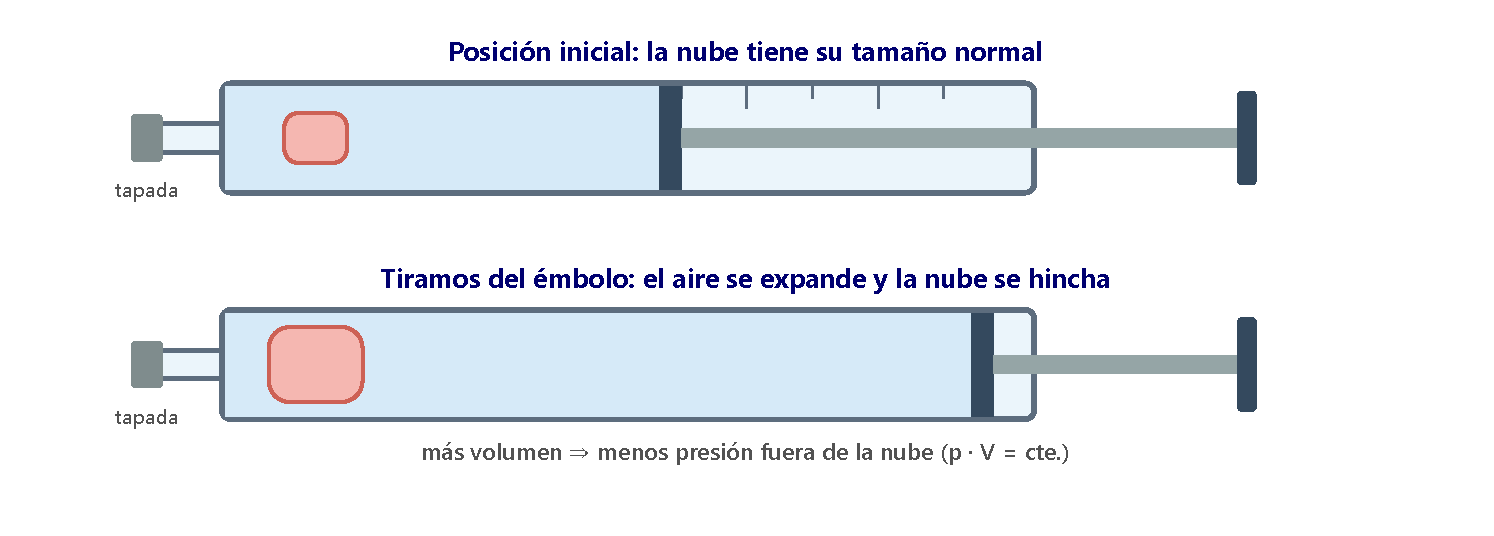
\includegraphics[width=0.85\textwidth]{images/UD1/practica_boyle}
    \caption{Al tirar del émbolo con la boquilla tapada, el aire de la jeringuilla se expande, su presión baja y la nube se
    hincha.}
    \label{fig:ud1-practica-boyle}
\end{figure}

\begin{exercise}
    a) Explica qué le sucede a la nube en cada parte del experimento. b) Utiliza la ley de Boyle-Mariotte para justificarlo.
    \begin{solu}
        a) \textcolor{red}{Al tirar del émbolo la nube se hincha mucho; al empujarlo, se encoge}; en ambos casos recupera su tamaño al
        volver a la posición inicial. b) \textcolor{blue}{La nube está llena de burbujas de aire. Al tirar del émbolo aumenta el volumen
        de la jeringuilla y, como \(p V\) es constante a temperatura constante, la presión del aire que rodea la nube baja.} El
        aire de las burbujas, a más presión que el de fuera, se expande hasta igualar presiones: \textcolor{red}{la nube crece}. Al
        empujar el émbolo ocurre lo contrario: sube la presión y el aire de las burbujas se comprime.
    \end{solu}
\end{exercise}

\subsection{¿Qué tienen que ver los tsunamis con los gases?}

\begin{multicols}{2}
    \textbf{Objetivo}
    \begin{itemize}
        \item Observar cómo un cambio de temperatura de un gas produce un cambio de presión capaz de mover agua.
    \end{itemize}
    \columnbreak
    \textbf{Material y reactivos}
    \begin{itemize}
        \item Plato hondo, vaso de vidrio estrecho, mechero de cocina.
        \item Alcohol de 70°, colorante alimentario y agua.
    \end{itemize}
\end{multicols}

\textbf{Procedimiento}
\begin{enumerate}[label=\numberballgreen]
    \item Echa agua en el plato hasta cubrir dos dedos de profundidad, añade dos gotas de colorante y remueve.
    \item Humedece con un poco de alcohol el interior del vaso y enciéndelo con el mechero. \textbf{Hazlo con un adulto y lejos de
    materiales que puedan arder.}
    \item Coloca enseguida el vaso boca abajo en el plato y observa lo que sucede (puedes grabarlo en vídeo y verlo a cámara
    lenta).
\end{enumerate}

\begin{exercise}
    a) Describe lo que ocurre. b) Explica, con las leyes de los gases, por qué sube el agua dentro del vaso.
    c) Busca información: ¿cómo se forman los tsunamis reales? ¿Tendría sentido un sistema de alerta de tsunamis en España?
    \begin{solu}
        a) \textcolor{red}{La llama se apaga y el agua del plato entra con rapidez en el vaso}, formando una «ola» en el plato.
        b) \textcolor{blue}{La combustión calienta el aire del vaso. Al apagarse la llama, el gas se enfría a volumen casi constante y,
        por la ley de Gay-Lussac, su presión baja} (además, parte del vapor de agua formado se condensa). \textcolor{red}{La presión
        atmosférica, mayor que la del interior, empuja el agua hacia dentro} hasta igualar presiones.
        c) \textcolor{red}{Los tsunamis se producen sobre todo por terremotos submarinos} que desplazan bruscamente grandes masas de agua;
        también por erupciones o deslizamientos. Sí tiene sentido: el golfo de Cádiz y el Mediterráneo han sufrido tsunamis
        (como el que siguió al terremoto de Lisboa de 1755), y España cuenta con un sistema de alerta.
    \end{solu}
\end{exercise}

%========================================================================================
\section{Situación de aprendizaje: mujeres y ciencia (ODS 5)}\label{sec:ud1-ods}
%========================================================================================

El \textbf{Objetivo de Desarrollo Sostenible 5} busca la \textbf{igualdad de género}: que mujeres y niñas tengan los mismos
derechos y oportunidades que los hombres y vivan libres de violencia. La Declaración Universal de los Derechos Humanos de 1948
ya afirmaba que todos los seres humanos nacen libres e iguales en dignidad y derechos. Sin embargo, todavía hay países sin
leyes que protejan la igualdad, y en la ciencia la desigualdad sigue siendo visible: hasta 2023, menos de 30 mujeres habían
recibido un premio Nobel de Física, Química o Medicina, frente a varios cientos de hombres, y en el mundo menos del 30\,\% de
las personas que investigan son mujeres.

\begin{marker}
    \textbf{Reto:} analizad la presencia de las mujeres en la ciencia y proponed medidas para reducir la brecha de género en
    las materias científicas de vuestro centro.
\end{marker}

\begin{enumerate}[label=\numberballred]
    \item \textbf{Veo, pienso, me pregunto.} Buscad titulares recientes sobre mujeres y ciencia (premios Nobel, puestos de
    dirección en investigación, porcentaje de investigadoras). De forma individual, anotad qué veis, qué pensáis y qué preguntas
    os surgen.
    \item \textbf{Investigación.} Elegid a una de las mujeres premiadas con el Nobel de Química o de Física (Marie Curie,
    Irène Joliot-Curie, Dorothy Crowfoot Hodgkin, Ada Yonath, Frances Arnold, Emmanuelle Charpentier, Jennifer Doudna,
    Donna Strickland, Andrea Ghez, Anne L'Huillier…). ¿Por qué recibió el premio? ¿Qué dificultades encontró?
    \item \textbf{Análisis.} ¿Qué opináis de que tan pocos premios científicos hayan sido para mujeres? ¿Cuál creéis que es
    el motivo principal? ¿Ocurre lo mismo en todas las disciplinas?
    \item \textbf{Propuesta.} Redactad un plan de medidas concretas para que en vuestro centro haya un porcentaje igualitario de
    chicas y chicos en las materias científicas, y presentadlo al resto de la clase.
\end{enumerate}

    \newpage
    %! Unidad 1 — Leyes fundamentales de la química: ejercicios resueltos y ejercicios finales
%! Fuente: Fuentes/Quimica/Unidad 1 («Ejercicios resueltos», «Practica y calcula», «Piensa y resuelve»).
%! Enunciados adaptados con datos cambiados; soluciones recalculadas. Dificultad: \(\star\) baja, \(\star\star\) media, \(\star\star\star\) alta.

\section{Ejercicios resueltos}\label{sec:ud1-resueltos}

Salvo que se indique otra cosa, usa las masas atómicas H = 1; C = 12; N = 14; O = 16; Na = 23; S = 32; Cl = 35,5;
Fe = 55,8; y \(R = \qty{0.082}{\atm\litre\per\mole\per\kelvin}\).

\begin{example}
    \textbf{Óxidos de hierro.} Se analizan cuatro muestras de óxidos de hierro con estos resultados:
    \begin{itemize}
        \item Muestra A: \qty{8}{\gram} de óxido con un 70\,\% de hierro.
        \item Muestra B: \qty{20}{\gram} de óxido, de los que \qty{14}{\gram} son de hierro.
        \item Muestra C: \qty{4.2}{\gram} de hierro y \qty{1.2}{\gram} de oxígeno.
        \item Muestra D: \qty{2}{\gram} de óxido, de los que \qty{0.6}{\gram} son de oxígeno.
    \end{itemize}
    a) Organiza los datos en una tabla con las masas de hierro, oxígeno y óxido. b) ¿Se trata siempre del mismo óxido?
    c) ¿Qué masa de oxígeno se necesita para que \qty{21}{\gram} de hierro formen un óxido como el de la muestra C?

    \textbf{Solución.} a) Usamos la ley de conservación de la masa, \(m_{\ch{Fe}} + m_{\ch{O}} = m_{\text{óxido}}\):
    A: \(m_{\ch{Fe}} = \num{0.70} \cdot 8 = \qty{5.6}{\gram}\) y \(m_{\ch{O}} = \qty{2.4}{\gram}\); B: \(m_{\ch{O}} = 20 - 14 = \qty{6}{\gram}\);
    C: \(m_{\text{óxido}} = \num{4.2} + \num{1.2} = \qty{5.4}{\gram}\); D: \(m_{\ch{Fe}} = 2 - \num{0.6} = \qty{1.4}{\gram}\).
    \begin{center}
        \begin{tabular}{@{}cccc@{}}
            \toprule
            \textbf{Muestra} & \textbf{Hierro (g)} & \textbf{Oxígeno (g)} & \textbf{Óxido (g)} \\
            \midrule
            A & 5,6 & 2,4 & 8 \\[3pt]
            B & 14 & 6 & 20 \\[3pt]
            C & 4,2 & 1,2 & 5,4 \\[3pt]
            D & 1,4 & 0,6 & 2 \\
            \bottomrule
        \end{tabular}
    \end{center}
    b) Calculamos la proporción \(m_{\ch{Fe}}/m_{\ch{O}}\): A \(\num{5.6}/\num{2.4} = \num{2.33}\); B \(14/6 = \num{2.33}\);
    C \(\num{4.2}/\num{1.2} = \num{3.5}\); D \(\num{1.4}/\num{0.6} = \num{2.33}\). Por la ley de Proust, A, B y D son el mismo óxido;
    C es otro diferente.

    c) En el óxido C, \(\dfrac{m_{\ch{Fe}}}{m_{\ch{O}}} = \num{3.5} \Rightarrow m_{\ch{O}} = \dfrac{21}{\num{3.5}} = \qty{6}{\gram}\) de oxígeno.
\end{example}

\begin{example}
    \textbf{Amoníaco.} Una muestra contiene \qty{85}{\gram} de amoníaco, \ch{NH3}. Calcula: a) la masa molecular; b) los moles;
    c) las moléculas; d) el número total de átomos; e) los átomos de nitrógeno y de hidrógeno; f) la composición centesimal.

    \textbf{Solución.} a) \(M(\ch{NH3}) = 14 + 3 \cdot 1 = \qty{17}{\uma}\) (\(M = \qty{17}{\gram\per\mole}\)).

    b) \(\qty{85}{\gram} \cdot \dfrac{\qty{1}{\mole}}{\qty{17}{\gram}} = \qty{5}{\mole}\).
    c) \(\qty{5}{\mole} \cdot \num{6.022e23} = \num{3.011e24}\) moléculas.

    d) Cada molécula tiene 4 átomos: \(4 \cdot \num{3.011e24} = \num{1.204e25}\) átomos.

    e) Un átomo de N y tres de H por molécula: \(\num{3.011e24}\) átomos de N y \(3 \cdot \num{3.011e24} = \num{9.033e24}\) de H.

    f) \(\%\,\ch{N} = \dfrac{14}{17} \cdot 100 = \qty{82.35}{\percent}\); \(\%\,\ch{H} = \dfrac{3}{17} \cdot 100 = \qty{17.65}{\percent}\).
\end{example}

\begin{example}
    \textbf{Leyes de los gases.} Un recipiente de \qty{5}{\litre} contiene un gas a \qty{2}{\atm} y \qty{60}{\degreeCelsius}.
    Indica qué ley aplicas en cada caso y calcula: a) el volumen si se duplica la temperatura absoluta a presión constante;
    b) la temperatura si la presión se reduce a la mitad sin cambiar el volumen; c) la presión si, a temperatura constante, el
    volumen pasa a ser \qty{25}{\litre}.

    \textbf{Solución.} Datos: \(V_1 = \qty{5}{\litre}\), \(p_1 = \qty{2}{\atm}\), \(T_1 = 60 + 273 = \qty{333}{\kelvin}\).

    a) Ley de Charles: \(\dfrac{V_1}{T_1} = \dfrac{V_2}{T_2} \Rightarrow V_2 = V_1 \dfrac{2 T_1}{T_1} = 2 \cdot 5 = \qty{10}{\litre}\).

    b) Ley de Gay-Lussac: \(\dfrac{p_1}{T_1} = \dfrac{p_2}{T_2} \Rightarrow T_2 = T_1 \dfrac{p_1/2}{p_1} = \dfrac{333}{2} = \qty{166.5}{\kelvin}\).

    c) Ley de Boyle-Mariotte: \(p_2 = \dfrac{p_1 V_1}{V_2} = \dfrac{2 \cdot 5}{25} = \qty{0.4}{\atm}\).
\end{example}

\begin{example}
    \textbf{¿Qué gas es?} a) La densidad de un gas es \qty{1.16}{\gram\per\litre} a \qty{750}{\mmHg} y \qty{15}{\degreeCelsius}.
    Averigua si es monóxido de carbono, \ch{CO}, monóxido de azufre, \ch{SO}, o amoníaco, \ch{NH3}. b) ¿Cuál sería la densidad de
    los otros dos gases en esas condiciones? c) ¿A qué presión la densidad del gas sería \qty{0.6}{\gram\per\litre} a
    \qty{30}{\degreeCelsius}?

    \textbf{Solución.} Datos: \(p = 750/760 = \qty{0.987}{\atm}\), \(T = \qty{288}{\kelvin}\).

    a) De \(p V = \dfrac{m}{M} R T\) y \(d = m/V\):
    \[ M = \frac{d R T}{p} = \frac{\num{1.16} \cdot \num{0.082} \cdot 288}{\num{0.987}} = \qty{27.8}{\gram\per\mole} \approx 28 \] Como \(M(\ch{CO}) = \qty{28}{\gram\per\mole}\), \(M(\ch{SO}) = 48\) y
    \(M(\ch{NH3}) = 17\), el gas es \textbf{monóxido de carbono}.

    b) \(d = \dfrac{p M}{R T}\): \ch{SO}: \(\dfrac{\num{0.987} \cdot 48}{\num{0.082} \cdot 288} = \qty{2.01}{\gram\per\litre}\);
    \ch{NH3}: \(\dfrac{\num{0.987} \cdot 17}{\num{0.082} \cdot 288} = \qty{0.71}{\gram\per\litre}\).

    c) \(p = \dfrac{d R T}{M} = \dfrac{\num{0.6} \cdot \num{0.082} \cdot 303}{28} = \qty{0.53}{\atm}\).
\end{example}

\begin{example}
    \textbf{Mezcla de vapores.} En un recipiente de \qty{10}{\litre} se introducen \qty{9.2}{\gram} de etanol, \ch{CH3CH2OH}, y
    \qty{11.6}{\gram} de acetona, \ch{CH3COCH3}. Después de cerrarlo, se calienta hasta \qty{280}{\degreeCelsius}, temperatura muy
    superior a los puntos de ebullición de ambos líquidos. Calcula: a) la presión parcial del etanol; b) la de la acetona; c) la
    presión total.

    \textbf{Solución.} Cada gas se comporta como si estuviera solo en los \qty{10}{\litre} (ley de Dalton). \(T = \qty{553}{\kelvin}\).
    \(n_{\text{etanol}} = \dfrac{\num{9.2}}{46} = \qty{0.2}{\mole}\); \(n_{\text{acetona}} = \dfrac{\num{11.6}}{58} = \qty{0.2}{\mole}\).

    a) y b) \(p = \dfrac{n R T}{V} = \dfrac{\num{0.2} \cdot \num{0.082} \cdot 553}{10} = \qty{0.907}{\atm}\) para cada uno, porque hay los
    mismos moles de los dos.

    c) \(p_T = \num{0.907} + \num{0.907} = \qty{1.81}{\atm}\). También se puede calcular con los moles totales:
    \(p_T = \dfrac{\num{0.4} \cdot \num{0.082} \cdot 553}{10} = \qty{1.81}{\atm}\).
\end{example}

%========================================================================================
\section{Ejercicios de aplicación}\label{sec:ud1-aplicacion}
%========================================================================================

\subsection{Leyes ponderales y volumétricas}

\begin{exercise}
    \(\star\) Completa la tabla de la reacción entre hierro y azufre para formar sulfuro de hierro(II),
    \(\ch{Fe(s) + S(s) -> FeS(s)}\), sabiendo que en la primera fila reaccionan exactamente las masas indicadas.
    \begin{center}
        \begin{tabular}{@{}ccc@{}}
            \toprule
            \(m\)\textbf{(Fe) (g)} & \(m\)\textbf{(S) (g)} & \(m\)\textbf{(FeS) (g)} \\
            \midrule
            55,8 & 32 & A \\[3pt]
            80 & B & C \\[3pt]
            D & 15 & E \\
            \bottomrule
        \end{tabular}
    \end{center}
    \begin{solu}
        \textcolor{blue}{Proporción \(m_{\ch{Fe}}/m_{\ch{S}} = \num{55.8}/32 = \num{1.744}\).}
        \(A = \num{55.8} + 32 = \textcolor{red}{\num{87.8}}\); \(B = 80/\num{1.744} = \textcolor{red}{\num{45.9}}\);
        \(C = 80 + \num{45.9} = \textcolor{red}{\num{125.9}}\); \(D = 15 \cdot \num{1.744} = \textcolor{red}{\num{26.2}}\);
        \(E = \num{26.2} + 15 = \textcolor{red}{\num{41.2}}\) (en gramos).
    \end{solu}
\end{exercise}

\begin{exercise}
    \(\star\star\) Al reaccionar completamente \qty{4}{\gram} de una sustancia A con \qty{6}{\gram} de otra B se forman
    \qty{10}{\gram} de un compuesto C. ¿Qué masa de C se obtendrá si se mezclan \qty{10}{\gram} de A con \qty{12}{\gram} de B?
    ¿Sobrará algún reactivo?
    \begin{solu}
        \textcolor{blue}{Proporción A:B = 4:6. Para 10 g de A harían falta 15 g de B, y solo hay 12 g: B se agota.} Con 12 g de B
        reaccionan \(12 \cdot 4/6 = \qty{8}{\gram}\) de A. Se forman \(8 + 12 = \textcolor{red}{\qty{20}{\gram}}\) de C y
        \textcolor{red}{sobran \qty{2}{\gram} de A}.
    \end{solu}
\end{exercise}

\begin{exercise}
    \(\star\star\) El azufre y el oxígeno forman dióxido de azufre combinándose en la proporción en masa 1:1. Completa la tabla
    (\(m_{\text{exc}}\) es la masa de reactivo que sobra) e indica qué ley ponderal se cumple.
    \begin{center}
        \begin{tabular}{@{}cccccc@{}}
            \toprule
            \textbf{Experiencia} & \(m\)\textbf{(S)} & \(m\)\textbf{(O)} & \(m\)\textbf{(\ch{SO2})} & \(m_{\text{exc}}\)\textbf{(S)} & \(m_{\text{exc}}\)\textbf{(O)} \\
            \midrule
            1 & 4 & 4 & 8 & 0 & 0 \\[3pt]
            2 & 5 & 7 & A & B & 2 \\[3pt]
            3 & C & 7 & 12 & 1 & D \\[3pt]
            4 & 9 & 4 & E & F & G \\
            \bottomrule
        \end{tabular}
    \end{center}
    \begin{solu}
        \textcolor{blue}{Ley de Proust: siempre reaccionan masas iguales de S y de O.}
        Exp. 2: reaccionan 5 g de S y 5 g de O: \(A = \textcolor{red}{10}\), \(B = \textcolor{red}{0}\).
        Exp. 3: 12 g de \ch{SO2} son 6 g de S y 6 g de O: \(D = 7 - 6 = \textcolor{red}{1}\), \(C = 6 + 1 = \textcolor{red}{7}\).
        Exp. 4: el O se agota: \(E = \textcolor{red}{8}\), \(F = 9 - 4 = \textcolor{red}{5}\), \(G = \textcolor{red}{0}\) (en gramos).
    \end{solu}
\end{exercise}

\begin{exercise}
    \(\star\star\) El plomo y el cloro forman dos compuestos. En una muestra del primero hay \qty{0.5836}{\gram} de Pb y
    \qty{0.200}{\gram} de Cl; en una del segundo, \qty{0.4377}{\gram} de Pb y \qty{0.300}{\gram} de Cl.
    a) Halla la proporción entre Pb y Cl en cada muestra. b) Si el primer compuesto es \ch{PbCl2}, ¿cuál es el segundo?
    c) ¿Cuántos gramos de cloro deben reaccionar con \qty{60}{\gram} de Pb para formar cada compuesto?
    \begin{solu}
        a) Primero: \(\num{0.5836}/\num{0.200} = \textcolor{red}{\num{2.918}}\); segundo: \(\num{0.4377}/\num{0.300} = \textcolor{red}{\num{1.459}}\).
        b) \textcolor{blue}{Con la misma masa de Pb, el segundo tiene el doble de cloro} (\(\num{2.918}/\num{1.459} = 2\)):
        \textcolor{red}{\ch{PbCl4}}.
        c) \(60/\num{2.918} = \textcolor{red}{\qty{20.6}{\gram}}\) de Cl para el primero y \(60/\num{1.459} = \textcolor{red}{\qty{41.1}{\gram}}\)
        para el segundo.
    \end{solu}
\end{exercise}

\begin{exercise}
    \(\star\star\) En el amoníaco, el nitrógeno y el hidrógeno están en la proporción en masa 14:3. a) ¿Qué masa de hidrógeno
    hay que añadir para que reaccionen \qty{120}{\gram} de nitrógeno? b) ¿Cuánto amoníaco se obtiene? c) ¿Cuánto amoníaco
    se obtiene con \qty{90}{\gram} de hidrógeno y \qty{40}{\gram} de nitrógeno? ¿Sobra algo?
    \begin{solu}
        a) \(m_{\ch{H}} = 120 \cdot 3/14 = \textcolor{red}{\qty{25.7}{\gram}}\). b) \(120 + \num{25.7} = \textcolor{red}{\qty{145.7}{\gram}}\) de \ch{NH3}.
        c) \textcolor{blue}{Para 40 g de N bastan \(40 \cdot 3/14 = \qty{8.57}{\gram}\) de H: el N se agota.} Se forman
        \(40 + \num{8.57} = \textcolor{red}{\qty{48.6}{\gram}}\) de \ch{NH3} y \textcolor{red}{sobran \qty{81.4}{\gram} de hidrógeno}.
    \end{solu}
\end{exercise}

\begin{exercise}
    \(\star\star\) El cobre y el oxígeno forman dos óxidos. En el óxido A la proporción en masa Cu:O es 3,97:1 y en el óxido B es
    7,94:1. a) Comprueba que se cumple la ley de las proporciones múltiples. b) Si A tiene un átomo de Cu por cada átomo de O,
    ¿cuál es la fórmula de B?
    \begin{solu}
        a) \textcolor{blue}{Con 1 g de O se combinan 3,97 g de Cu en A y 7,94 g en B:} \(\num{7.94}/\num{3.97} = \textcolor{red}{2}\), número entero
        sencillo. b) \textcolor{blue}{B tiene el doble de cobre por cada átomo de oxígeno:} \textcolor{red}{\ch{Cu2O}}.
    \end{solu}
\end{exercise}

\begin{exercise}
    \(\star\star\) Tras una excursión se recogen dos muestras de un mineral de cromo y oxígeno: la primera contiene
    \qty{52.0}{\gram} de Cr y \qty{24.0}{\gram} de O, y la segunda, \qty{39.0}{\gram} de Cr y \qty{18.0}{\gram} de O. ¿Se trata del
    mismo compuesto?
    \begin{solu}
        \(\num{52.0}/\num{24.0} = \num{2.167}\) y \(\num{39.0}/\num{18.0} = \num{2.167}\): \textcolor{red}{la proporción es la misma, luego es el
        mismo compuesto} (ley de Proust).
    \end{solu}
\end{exercise}

\begin{exercise}
    \(\star\) Un litro de hidrógeno reacciona con un litro de cloro para dar dos litros de cloruro de hidrógeno. ¿Cuántos litros
    de \ch{HCl} se obtienen si reaccionan \qty{6}{\litre} de hidrógeno con \qty{9}{\litre} de cloro? ¿Sobra algo? (Todos los
    volúmenes, en las mismas condiciones.)
    \begin{solu}
        \textcolor{blue}{Relación 1:1:2; el \ch{H2} se agota.} Se obtienen \(2 \cdot 6 = \textcolor{red}{\qty{12}{\litre}}\) de \ch{HCl} y
        \textcolor{red}{sobran \qty{3}{\litre} de \ch{Cl2}}.
    \end{solu}
\end{exercise}

\begin{exercise}
    \(\star\star\) Dos litros de nitrógeno reaccionan con seis litros de hidrógeno y dan cuatro litros de amoníaco; un litro de
    hidrógeno con uno de cloro da dos litros de cloruro de hidrógeno. ¿Contradicen estas reacciones la ley de Lavoisier?
    \begin{solu}
        \textcolor{red}{No.} \textcolor{blue}{La ley de Lavoisier se refiere a la masa, no al volumen. En la primera reacción el volumen
        disminuye (\(8 \to 4\) L) porque el número de moléculas disminuye (\(\ch{N2 + 3 H2 -> 2 NH3}\)), y en la segunda no cambia;
        pero en ambas los átomos se conservan y, por tanto, la masa también.}
    \end{solu}
\end{exercise}

\begin{exercise}
    \(\star\star\) El azufre gaseoso y el oxígeno forman tres óxidos; las relaciones de volumen S:\ch{O2} son 2:1, 1:1 y 2:3.
    a) ¿Qué volúmenes de azufre y de oxígeno hacen falta para obtener \qty{3}{\litre} de cada óxido (si se obtiene un volumen de
    óxido igual al de azufre)? b) ¿Cuál es la fórmula de cada óxido?
    \begin{solu}
        a) \textcolor{red}{3 L de S con 1,5 L, 3 L y 4,5 L de \ch{O2}}, respectivamente.
        b) \textcolor{blue}{Cada molécula de óxido lleva un átomo de S, y cada molécula de \ch{O2} aporta 2 átomos de O:}
        \textcolor{red}{\ch{SO}, \ch{SO2} y \ch{SO3}}.
    \end{solu}
\end{exercise}

\begin{exercise}
    \(\star\star\) El hidrógeno reacciona con el oxígeno para dar vapor de agua: \ch{2 H2(g) + O2(g) -> 2 H2O(g)}. Completa
    la tabla de volúmenes (en litros, en las mismas condiciones).
    \begin{center}
        \begin{tabular}{@{}ccccc@{}}
            \toprule
            \multicolumn{2}{c}{\textbf{Inicial}} & \multicolumn{3}{c}{\textbf{Final}} \\
            \cmidrule(r){1-2} \cmidrule(l){3-5}
            \ch{H2} & \ch{O2} & \ch{H2O} & \ch{H2} & \ch{O2} \\
            \midrule
            4 & 2 & 4 & 0 & 0 \\[3pt]
            6 & 4 & A & 0 & B \\[3pt]
            C & 3 & 6 & 0 & 0 \\[3pt]
            10 & 3 & D & E & 0 \\
            \bottomrule
        \end{tabular}
    \end{center}
    \begin{solu}
        \(A = \textcolor{red}{6}\), \(B = 4 - 3 = \textcolor{red}{1}\); \(C = \textcolor{red}{6}\); \textcolor{blue}{en la última fila se agota el \ch{O2}:}
        \(D = \textcolor{red}{6}\), \(E = 10 - 6 = \textcolor{red}{4}\).
    \end{solu}
\end{exercise}

\subsection{Cantidad de sustancia}

\begin{exercise}
    \(\star\) Indica si son verdaderas o falsas: a) La masa de un mol de \ch{O2} es \qty{16}{\gram}. b) En condiciones normales,
    un mol de \ch{CO2} y un mol de \ch{CH4} ocupan el mismo volumen. c) Un mol de \ch{H2O} y un mol de \ch{NH3} contienen el mismo
    número de átomos.
    \begin{solu}
        a) \textcolor{red}{F}: es \qty{32}{\gram}. b) \textcolor{red}{V}: ley de Avogadro. c) \textcolor{red}{F}: el mismo número de moléculas,
        pero cada molécula de agua tiene 3 átomos y cada una de amoníaco, 4.
    \end{solu}
\end{exercise}

\begin{exercise}
    \(\star\) Completa la tabla.
    \begin{center}
        \begin{tabular}{@{}cccc@{}}
            \toprule
            \textbf{Sustancia} & \textbf{Moles} & \textbf{Masa (g)} & \textbf{Moléculas} \\
            \midrule
            \ch{H2} & 3 & A & B \\[3pt]
            \ch{N2} & C & 70 & D \\[3pt]
            \ch{O2} & E & F & \num{2.4e24} \\[3pt]
            \ch{H2O} & 1,5 & G & H \\
            \bottomrule
        \end{tabular}
    \end{center}
    \begin{solu}
        \(A = 3 \cdot 2 = \textcolor{red}{6}\); \(B = 3 \cdot \num{6.022e23} = \textcolor{red}{\num{1.81e24}}\);
        \(C = 70/28 = \textcolor{red}{\num{2.5}}\); \(D = \textcolor{red}{\num{1.51e24}}\);
        \(E = \num{2.4e24}/\num{6.022e23} = \textcolor{red}{\num{3.99}}\); \(F = \num{3.99} \cdot 32 = \textcolor{red}{\num{127.5}}\);
        \(G = \num{1.5} \cdot 18 = \textcolor{red}{27}\); \(H = \textcolor{red}{\num{9.03e23}}\).
    \end{solu}
\end{exercise}

\begin{exercise}
    \(\star\) La cafeína, \ch{C8H10N4O2}, está presente en el café, el té y muchos refrescos. Un frasco de un laboratorio
    contiene \qty{50}{\gram} de cafeína. Calcula: a) los moles; b) las moléculas; c) la composición centesimal; d) los átomos de
    carbono y de nitrógeno.
    \begin{solu}
        \(M = \qty{194}{\gram\per\mole}\). a) \(50/194 = \textcolor{red}{\qty{0.258}{\mole}}\). b) \(\textcolor{red}{\num{1.55e23}}\) moléculas.
        c) \textcolor{red}{C \qty{49.5}{\percent}, H \qty{5.15}{\percent}, N \qty{28.9}{\percent}, O \qty{16.5}{\percent}}.
        d) C: \(8 \cdot \num{1.55e23} = \textcolor{red}{\num{1.24e24}}\); N: \(4 \cdot \num{1.55e23} = \textcolor{red}{\num{6.21e23}}\).
    \end{solu}
\end{exercise}

\begin{exercise}
    \(\star\star\) La nicotina, \ch{C10H14N2}, es la sustancia adictiva del tabaco. Una muestra contiene \num{2.5e25} átomos de
    carbono. Calcula: a) las moléculas de nicotina; b) la composición centesimal; c) los átomos de nitrógeno; d) los moles;
    e) la masa de la muestra.
    \begin{solu}
        a) \(\num{2.5e25}/10 = \textcolor{red}{\num{2.5e24}}\). b) \(M = \qty{162}{\gram\per\mole}\): \textcolor{red}{C \qty{74.1}{\percent}, H \qty{8.6}{\percent},
        N \qty{17.3}{\percent}}. c) \(2 \cdot \num{2.5e24} = \textcolor{red}{\num{5e24}}\). d) \(\num{2.5e24}/\num{6.022e23} = \textcolor{red}{\qty{4.15}{\mole}}\).
        e) \(\num{4.15} \cdot 162 = \textcolor{red}{\qty{673}{\gram}}\).
    \end{solu}
\end{exercise}

\begin{exercise}
    \(\star\star\) ¿Cuál de estas muestras tiene mayor número de átomos? a) \qty{25}{\gram} de Fe. b) \num{4e23} moléculas de
    \ch{NH3}. c) \qty{1.2}{\mole} de \ch{CO2}.
    \begin{solu}
        a) \(25/\num{55.8} \cdot \num{6.022e23} = \num{2.70e23}\); b) \(4 \cdot \num{4e23} = \num{1.6e24}\);
        c) \(3 \cdot \num{1.2} \cdot \num{6.022e23} = \num{2.17e24}\). \textcolor{red}{La muestra c}.
    \end{solu}
\end{exercise}

\begin{exercise}
    \(\star\star\) Una gota de agua ocupa unos \qty{0.05}{\cubic\centi\metre}. ¿Cuántas moléculas de agua hay en 15 gotas? (Densidad
    del agua: \qty{1}{\gram\per\cubic\centi\metre}.)
    \begin{solu}
        \(m = 15 \cdot \num{0.05} = \qty{0.75}{\gram}\); \(N = \dfrac{\num{0.75}}{18} \cdot \num{6.022e23} = \textcolor{red}{\num{2.51e22}}\) moléculas.
    \end{solu}
\end{exercise}

\begin{exercise}
    \(\star\star\) Calcula: a) los gramos de fósforo que hay en \qty{2.4}{\mole} de fosfano, \ch{PH3}; b) los átomos de oxígeno en
    \qty{9.45}{\gram} de ácido nítrico, \ch{HNO3}; c) los moles de átomos de oxígeno en \qty{3.5}{\mole} de \ch{Al2(SO4)3}.
    \begin{solu}
        a) \(\num{2.4} \cdot 31 = \textcolor{red}{\qty{74.4}{\gram}}\). b) \(M = \qty{63}{\gram\per\mole}\): \(\dfrac{\num{9.45}}{63} \cdot 3 \cdot \num{6.022e23} =
        \textcolor{red}{\num{2.71e23}}\). c) \textcolor{blue}{12 átomos de O por fórmula:} \(12 \cdot \num{3.5} = \textcolor{red}{\qty{42}{\mole}}\).
    \end{solu}
\end{exercise}

\subsection{Fórmula empírica y molecular}

\begin{exercise}
    \(\star\) Calcula la composición centesimal del fosfato de calcio, \ch{Ca3(PO4)2}. (Ca = 40; P = 31.)
    \begin{solu}
        \(M = 3 \cdot 40 + 2 \cdot 31 + 8 \cdot 16 = \qty{310}{\gram\per\mole}\).
        \textcolor{red}{Ca \qty{38.7}{\percent}; P \qty{20.0}{\percent}; O \qty{41.3}{\percent}}.
    \end{solu}
\end{exercise}

\begin{exercise}
    \(\star\star\) Una roca de \qty{40}{\kilogram} contiene un 80\,\% de carbonato de calcio, \ch{CaCO3}. Calcula: a) la masa de
    \ch{CaCO3}; b) la masa de oxígeno de la roca, si todo procede del carbonato.
    \begin{solu}
        a) \(\num{0.80} \cdot 40 = \textcolor{red}{\qty{32}{\kilogram}}\). b) \(M(\ch{CaCO3}) = \qty{100}{\gram\per\mole}\), con 48 g de O:
        \(32 \cdot \dfrac{48}{100} = \textcolor{red}{\qty{15.4}{\kilogram}}\).
    \end{solu}
\end{exercise}

\begin{exercise}
    \(\star\star\) Las plantas necesitan magnesio para fabricar la clorofila \textit{a}, de fórmula \ch{C55H72MgN4O5}. Calcula el
    porcentaje en masa de magnesio. (Mg = 24,3.)
    \begin{solu}
        \(M = \qty{892.3}{\gram\per\mole}\); \(\%\,\ch{Mg} = \dfrac{\num{24.3}}{\num{892.3}} \cdot 100 = \textcolor{red}{\qty{2.72}{\percent}}\).
    \end{solu}
\end{exercise}

\begin{exercise}
    \(\star\) Un óxido de hierro tiene un 72,4\,\% de hierro y un 27,6\,\% de oxígeno. Calcula su fórmula empírica.
    \begin{solu}
        Fe \(\num{72.4}/\num{55.8} = \num{1.297}\); O \(\num{27.6}/16 = \num{1.725}\) \(\rightarrow\) 1 : 1,33 \(\rightarrow\) (×3) 3 : 4.
        \textcolor{red}{\ch{Fe3O4}} (magnetita).
    \end{solu}
\end{exercise}

\begin{exercise}
    \(\star\) La glicina, el aminoácido más sencillo, contiene un 32,0\,\% de C, un 18,7\,\% de N, un 42,6\,\% de O y el resto de
    H. Calcula su fórmula empírica.
    \begin{solu}
        H: \qty{6.7}{\percent}. C \(\num{2.67}\); H \(\num{6.7}\); N \(\num{1.34}\); O \(\num{2.66}\) \(\rightarrow\) 2 : 5 : 1 : 2.
        \textcolor{red}{\ch{C2H5NO2}}.
    \end{solu}
\end{exercise}

\begin{exercise}
    \(\star\star\) La cafeína tiene un 49,5\,\% de C, un 5,15\,\% de H, un 28,9\,\% de N y un 16,5\,\% de O. Su masa molecular es 194.
    Determina su fórmula empírica y su fórmula molecular.
    \begin{solu}
        C \(\num{4.13}\); H \(\num{5.15}\); N \(\num{2.06}\); O \(\num{1.03}\) \(\rightarrow\) 4 : 5 : 2 : 1: empírica \textcolor{red}{\ch{C4H5N2O}}
        (\(M = 97\)). \(\alpha = 194/97 = 2\): molecular \textcolor{red}{\ch{C8H10N4O2}}.
    \end{solu}
\end{exercise}

\begin{exercise}
    \(\star\) Un compuesto gaseoso de carbono, hidrógeno y oxígeno tiene de fórmula molecular \ch{C2H6O}. Calcula: a) su fórmula
    empírica; b) los moles de moléculas en \qty{23}{\gram}; c) los gramos de carbono en \qty{23}{\gram}; d) los moles de átomos de
    oxígeno en \qty{23}{\gram}; e) los átomos de hidrógeno en \qty{23}{\gram}.
    \begin{solu}
        a) \textcolor{red}{\ch{C2H6O}} (no se puede simplificar). \(M = \qty{46}{\gram\per\mole}\). b) \(23/46 = \textcolor{red}{\qty{0.5}{\mole}}\).
        c) \(23 \cdot 24/46 = \textcolor{red}{\qty{12}{\gram}}\). d) \textcolor{red}{\qty{0.5}{\mole}}. e) \(6 \cdot \num{0.5} \cdot \num{6.022e23} = \textcolor{red}{\num{1.81e24}}\).
    \end{solu}
\end{exercise}

\begin{exercise}
    \(\star\star\) Un compuesto de nitrógeno y oxígeno contiene \qty{1.40}{\gram} de N por cada \qty{4.00}{\gram} de O. Su masa
    molecular es 108. Determina su fórmula molecular.
    \begin{solu}
        N \(\num{1.40}/14 = \num{0.10}\); O \(\num{4.00}/16 = \num{0.25}\) \(\rightarrow\) 1 : 2,5 \(\rightarrow\) 2 : 5: empírica \ch{N2O5}
        (\(M = 108\)). \(\alpha = 1\): \textcolor{red}{\ch{N2O5}}.
    \end{solu}
\end{exercise}

\begin{exercise}
    \(\star\star\) El benzoato de sodio (E-211) es un conservante alimentario. Contiene un 58,33\,\% de C, un 3,47\,\% de H, un
    22,22\,\% de O y un 15,97\,\% de Na. Su masa molecular relativa es 144. ¿Cuál es su fórmula molecular?
    \begin{solu}
        C \(\num{4.86}\); H \(\num{3.47}\); O \(\num{1.389}\); Na \(\num{0.694}\) \(\rightarrow\) 7 : 5 : 2 : 1; \(M = 144\), \(\alpha = 1\):
        \textcolor{red}{\ch{C7H5O2Na}}.
    \end{solu}
\end{exercise}

\begin{exercise}
    \(\star\star\) El paracetamol tiene un 63,58\,\% de C, un 5,96\,\% de H, un 9,27\,\% de N y un 21,19\,\% de O. Su masa molar es
    \qty{151}{\gram\per\mole}. ¿Cuál es su fórmula empírica? ¿Y la molecular?
    \begin{solu}
        C \(\num{5.30}\); H \(\num{5.96}\); N \(\num{0.662}\); O \(\num{1.324}\) \(\rightarrow\) 8 : 9 : 1 : 2.
        \textcolor{red}{Empírica y molecular: \ch{C8H9NO2}} (\(M = 151\), \(\alpha = 1\)).
    \end{solu}
\end{exercise}

\subsection{Leyes de los gases}

\begin{exercise}
    \(\star\) ¿Cómo debe variar la presión de un gas para que su volumen se reduzca a la tercera parte, a temperatura constante?
    \begin{solu}
        \textcolor{blue}{Boyle: \(p\) y \(V\) son inversamente proporcionales.} \textcolor{red}{La presión debe triplicarse.}
    \end{solu}
\end{exercise}

\begin{exercise}
    \(\star\) Un gas está en un recipiente rígido. ¿Qué le pasa a su presión si la temperatura absoluta se triplica?
    \begin{solu}
        \textcolor{blue}{Gay-Lussac, a volumen constante \(p/T\) es constante:} \textcolor{red}{la presión se triplica}.
    \end{solu}
\end{exercise}

\begin{exercise}
    \(\star\) Justifica si son verdaderas o falsas: a) Al duplicar la temperatura absoluta de un gas sin variar el volumen, la
    presión se duplica. b) Al calentar un gas a presión constante, su volumen disminuye. c) Si se reduce a la mitad el volumen
    de un gas a presión constante, su temperatura absoluta se duplica.
    \begin{solu}
        a) \textcolor{red}{V} (Gay-Lussac). b) \textcolor{red}{F}: aumenta (Charles). c) \textcolor{red}{F}: se reduce a la mitad (Charles).
    \end{solu}
\end{exercise}

\begin{exercise}
    \(\star\star\) Un globo aerostático, sin variar su volumen, reduce su presión a la mitad durante el ascenso. ¿Cómo ha
    cambiado su temperatura?
    \begin{solu}
        \(\dfrac{p_1}{T_1} = \dfrac{p_1/2}{T_2} \Rightarrow \textcolor{red}{T_2 = T_1/2}\): \textcolor{red}{la temperatura absoluta se reduce a la mitad.}
    \end{solu}
\end{exercise}

\begin{exercise}
    \(\star\star\) \qty{5}{\litre} de \ch{NH3}(g) están a \qty{4}{\atm}. Si, a temperatura constante, el volumen se multiplica por 4,
    ¿cuál será la presión?
    \begin{solu}
        \(p_2 = \dfrac{4 \cdot 5}{20} = \textcolor{red}{\qty{1}{\atm}}\).
    \end{solu}
\end{exercise}

\begin{exercise}
    \(\star\star\) Un globo inflado a \qty{2}{\atm} ocupa \qty{15}{\litre} y explota si su volumen supera los \qty{25}{\cubic\deci\metre}.
    Calcula su volumen si la presión baja hasta \qty{1.5}{\atm} a temperatura constante. ¿Explotará?
    \begin{solu}
        \(V_2 = \dfrac{2 \cdot 15}{\num{1.5}} = \textcolor{red}{\qty{20}{\litre}}\); \textcolor{red}{no explota} (\(20 < 25\)).
    \end{solu}
\end{exercise}

\begin{exercise}
    \(\star\star\) Un recipiente de \qty{250}{\cubic\centi\metre} contiene un gas a \qty{25}{\degreeCelsius} y \qty{3000}{\mmHg}.
    Manteniendo el volumen, ¿cuál será la presión si la temperatura baja hasta \qty{-10}{\degreeCelsius}?
    \begin{solu}
        \(p_2 = 3000 \cdot \dfrac{263}{298} = \qty{2648}{\mmHg} = \textcolor{red}{\qty{3.48}{\atm}}\).
    \end{solu}
\end{exercise}

\begin{exercise}
    \(\star\star\) Un contenedor de oxígeno resiste hasta \qty{40}{\atm}. Se llena a \qty{20}{\degreeCelsius} con una presión de
    \qty{11400}{\mmHg}. a) Representa la presión frente a la temperatura. b) ¿Qué ley se refleja en la gráfica? c) Calcula la
    presión si la temperatura sube a \qty{45}{\degreeCelsius}. d) ¿A qué temperatura explotaría?
    \begin{solu}
        \(p_1 = 11400/760 = \qty{15}{\atm}\), \(T_1 = \qty{293}{\kelvin}\).
        a) \textcolor{blue}{Una recta que pasa por el origen (con \(T\) en kelvin) de pendiente \(15/293 = \qty{0.0512}{\atm\per\kelvin}\):}
        \begin{center}
            \begin{tikzpicture}
                \begin{axis}[grafica, xlabel={\(T\) (\unit{\kelvin})}, ylabel={\(p\) (\unit{\atm})}, xmin=0, xmax=850, ymin=0, ymax=45]
                    \addplot[thick, blue, domain=0:800] {15/293*x};
                    \addplot[dashed, red] coordinates {(0,40) (781,40) (781,0)};
                    \addplot[only marks, mark=*, mark size=1.5pt] coordinates {(293,15) (318,16.28)};
                \end{axis}
            \end{tikzpicture}
        \end{center}
        b) \textcolor{red}{Ley de Gay-Lussac.} c) \(p_2 = 15 \cdot \dfrac{318}{293} = \textcolor{red}{\qty{16.3}{\atm}}\).
        d) \(T = 293 \cdot \dfrac{40}{15} = \qty{781}{\kelvin} = \textcolor{red}{\qty{508}{\degreeCelsius}}\).
    \end{solu}
\end{exercise}

\begin{exercise}
    \(\star\star\) La relación entre el volumen y la temperatura de un gas a presión constante es \(V/T = \qty{0.5}{\litre\per\kelvin}\).
    a) Haz una tabla \(V\)-\(T\) con cinco temperaturas. b) Represéntala. c) ¿Qué relación hay entre \(V\) y \(T\)? ¿Qué ley la describe?
    \begin{solu}
        a) Por ejemplo: \(T = 100, 200, 300, 400, 500\) K \(\rightarrow\) \(V = 50, 100, 150, 200, 250\) L.
        b) \textcolor{blue}{Recta que pasa por el origen de pendiente \qty{0.5}{\litre\per\kelvin}.}
        c) \textcolor{red}{Son directamente proporcionales: ley de Charles.}
    \end{solu}
\end{exercise}

\begin{exercise}
    \(\star\star\) Un globo aerostático tiene un volumen de \qty{2.5e5}{\cubic\deci\metre} antes de despegar, a \qty{30}{\degreeCelsius}.
    La temperatura baja \qty{1}{\degreeCelsius} cada \qty{200}{\metre} de altura. Calcula su volumen a \qty{2}{\kilo\metre} de altura,
    suponiendo que la presión no cambia.
    \begin{solu}
        \textcolor{blue}{A 2 km la temperatura ha bajado \qty{10}{\degreeCelsius}: \(T_2 = \qty{293}{\kelvin}\).}
        \(V_2 = \num{2.5e5} \cdot \dfrac{293}{303} = \textcolor{red}{\qty{2.42e5}{\litre}}\).
    \end{solu}
\end{exercise}

\subsection{Teoría cinético-molecular}

\begin{exercise}
    \(\star\) Explica con la teoría cinético-molecular cómo cambian las condiciones de las partículas de un gas encerrado si:
    a) reducimos el volumen del recipiente; b) aumentamos la temperatura a volumen constante; c) añadimos al recipiente un gas
    inerte (que no reacciona).
    \begin{solu}
        a) \textcolor{red}{Las partículas tienen menos espacio y chocan más a menudo con las paredes: sube la presión} (su velocidad media
        no cambia si \(T\) es constante). b) \textcolor{red}{Se mueven más deprisa y chocan con más frecuencia y más fuerza: sube la
        presión.} c) \textcolor{red}{Hay más partículas chocando con las paredes: aumenta la presión total}, aunque la presión parcial
        del primer gas no cambia.
    \end{solu}
\end{exercise}

\begin{exercise}
    \(\star\star\) Lucía se encuentra un globo y decide inflarlo más, pero acaba explotando. Argumenta cuál de estas afirmaciones
    explica lo que ha pasado: a) Al aumentar la cantidad de aire aumenta la temperatura del globo. b) El volumen del globo
    aumenta porque disminuye la presión. c) Al aumentar la cantidad de aire aumenta la presión interior.
    \begin{solu}
        a) \textcolor{red}{F}. b) \textcolor{red}{F}. c) \textcolor{red}{V}: \textcolor{blue}{con más partículas hay más choques contra la pared del globo; la goma se
        estira hasta que no resiste la presión.}
    \end{solu}
\end{exercise}

\subsection{Ecuación de los gases ideales}

\begin{exercise}
    \(\star\) ¿Qué volumen ocupan \qty{40}{\gram} de oxígeno en condiciones normales? ¿Y a \qty{1}{\atm} y \qty{30}{\degreeCelsius}?
    \begin{solu}
        \(n = 40/32 = \qty{1.25}{\mole}\). En c.\,n.: \(\num{1.25} \cdot \num{22.4} = \textcolor{red}{\qty{28}{\litre}}\).
        A \qty{30}{\degreeCelsius}: \(\num{1.25} \cdot \num{0.082} \cdot 303 = \textcolor{red}{\qty{31.1}{\litre}}\).
    \end{solu}
\end{exercise}

\begin{exercise}
    \(\star\star\) Determina el volumen, en unidades del SI, de un recipiente que contiene \qty{2.5}{\mole} de un gas a
    \qty{800}{\mmHg} y \qty{60}{\degreeCelsius}.
    \begin{solu}
        \(V = \dfrac{\num{2.5} \cdot \num{0.082} \cdot 333}{800/760} = \qty{64.9}{\litre} = \textcolor{red}{\qty{6.49e-2}{\cubic\metre}}\).
    \end{solu}
\end{exercise}

\begin{exercise}
    \(\star\star\) Halla la presión en un recipiente de \qty{30}{\cubic\metre} en el que hay \qty{56}{\gram} de nitrógeno, \ch{N2}, a
    \qty{-20}{\degreeCelsius}.
    \begin{solu}
        \(n = \qty{2}{\mole}\); \(V = \qty{30000}{\litre}\); \(p = \dfrac{2 \cdot \num{0.082} \cdot 253}{30000} = \textcolor{red}{\qty{1.38e-3}{\atm}}\):
        \textcolor{blue}{un gas muy enrarecido}.
    \end{solu}
\end{exercise}

\begin{exercise}
    \(\star\star\) Tenemos \qty{3}{\litre} de dióxido de carbono a \qty{820}{\mmHg} y \qty{27}{\degreeCelsius}. Calcula: a) el volumen que
    ocuparía en condiciones normales; b) los moles y las moléculas.
    \begin{solu}
        b) \(n = \dfrac{(820/760) \cdot 3}{\num{0.082} \cdot 300} = \textcolor{red}{\qty{0.132}{\mole}}\); \(N = \textcolor{red}{\num{7.92e22}}\) moléculas.
        a) \(V = \num{0.132} \cdot \num{22.4} = \textcolor{red}{\qty{2.95}{\litre}}\).
    \end{solu}
\end{exercise}

\begin{exercise}
    \(\star\star\) Una bombona de \qty{26}{\litre} contiene butano, \ch{C4H10}, a \qty{20}{\degreeCelsius}. Llena tiene una masa de
    \qty{24.0}{\kilogram}, y vacía, de \qty{22.5}{\kilogram}. a) Calcula la masa molar del butano y la masa de butano de la bombona.
    b) ¿Qué presión habría dentro si todo el butano estuviera en estado gaseoso?
    \begin{solu}
        a) \(M = 4 \cdot 12 + 10 = \textcolor{red}{\qty{58}{\gram\per\mole}}\); \(m = \textcolor{red}{\qty{1.5}{\kilogram}}\).
        b) \(n = 1500/58 = \qty{25.9}{\mole}\); \(p = \dfrac{\num{25.9} \cdot \num{0.082} \cdot 293}{26} = \textcolor{red}{\qty{23.9}{\atm}}\).
        \textcolor{blue}{(En realidad, a esa presión el butano se licúa: por eso las bombonas contienen butano líquido.)}
    \end{solu}
\end{exercise}

\begin{exercise}
    \(\star\) Un recipiente de \qty{3}{\cubic\deci\metre} contiene \qty{8}{\gram} de nitrógeno a \qty{30}{\degreeCelsius}. Calcula la presión.
    \begin{solu}
        \(p = \dfrac{(8/28) \cdot \num{0.082} \cdot 303}{3} = \textcolor{red}{\qty{2.37}{\atm}}\).
    \end{solu}
\end{exercise}

\begin{exercise}
    \(\star\) ¿Cuántos moles de \ch{CO2} hay en \qty{66}{\gram}? ¿Qué volumen ocupan a \qty{1}{\atm} y \qty{0}{\degreeCelsius}?
    \begin{solu}
        \(n = 66/44 = \textcolor{red}{\qty{1.5}{\mole}}\); \(V = \num{1.5} \cdot \num{22.4} = \textcolor{red}{\qty{33.6}{\litre}}\).
    \end{solu}
\end{exercise}

\begin{exercise}
    \(\star\star\) El kriptón, Kr(g), se almacena en una botella de \qty{15}{\litre} a \qty{10}{\atm} y \qty{20}{\degreeCelsius}. Calcula la
    masa de kriptón. (Kr = 83,8.)
    \begin{solu}
        \(n = \dfrac{10 \cdot 15}{\num{0.082} \cdot 293} = \qty{6.24}{\mole}\); \(m = \num{6.24} \cdot \num{83.8} = \textcolor{red}{\qty{523}{\gram}}\).
    \end{solu}
\end{exercise}

\begin{exercise}
    \(\star\star\) La presión dentro de un bote de laca es de \qty{4}{\bar} a \qty{25}{\degreeCelsius}. ¿Cuántos moles de gas hay en un bote de
    \qty{400}{\milli\litre}? ¿Y en uno de \qty{250}{\cubic\centi\metre}?
    \begin{solu}
        \(p = 4/\num{1.013} = \qty{3.95}{\atm}\). \(n_1 = \dfrac{\num{3.95} \cdot \num{0.4}}{\num{0.082} \cdot 298} = \textcolor{red}{\qty{0.065}{\mole}}\);
        \(n_2 = \textcolor{red}{\qty{0.040}{\mole}}\).
    \end{solu}
\end{exercise}

\begin{exercise}
    \(\star\star\) Una cantidad de gas ocupa \qty{1.5}{\litre} a cierta temperatura. ¿Cómo podríamos guardar esa misma cantidad en un
    recipiente de \qty{1}{\litre}? ¿Y en uno de \qty{5}{\litre}? La temperatura no cambia.
    \begin{solu}
        \textcolor{red}{En el de 1 L, comprimiéndolo: su presión aumenta 1,5 veces. En el de 5 L, el gas se expande hasta ocupar todo el
        recipiente y su presión se reduce a \(1{,}5/5 = 0{,}3\) veces la inicial} (ley de Boyle).
    \end{solu}
\end{exercise}

\subsection{Densidad de los gases}

\begin{exercise}
    \(\star\) ¿Cuál es la densidad del dióxido de azufre, \ch{SO2}, a \qty{120}{\degreeCelsius} y \qty{1.5}{\atm}?
    \begin{solu}
        \(d = \dfrac{p M}{R T} = \dfrac{\num{1.5} \cdot 64}{\num{0.082} \cdot 393} = \textcolor{red}{\qty{2.98}{\gram\per\litre}}\).
    \end{solu}
\end{exercise}

\begin{exercise}
    \(\star\) Calcula la densidad del metano, \ch{CH4}: a) a \qty{80}{\degreeCelsius} y \qty{900}{\mmHg}; b) en condiciones normales.
    \begin{solu}
        a) \(d = \dfrac{(900/760) \cdot 16}{\num{0.082} \cdot 353} = \textcolor{red}{\qty{0.655}{\gram\per\litre}}\).
        b) \(d = 16/\num{22.4} = \textcolor{red}{\qty{0.714}{\gram\per\litre}}\).
    \end{solu}
\end{exercise}

\begin{exercise}
    \(\star\star\) La densidad de un gas es \qty{2.5}{\gram\per\litre} a \qty{20}{\degreeCelsius} y \qty{1}{\atm}. ¿Cuál será a
    \qty{60}{\degreeCelsius} y \qty{1.5}{\atm}?
    \begin{solu}
        \textcolor{blue}{\(d\) es proporcional a \(p/T\):} \(d_2 = \num{2.5} \cdot \dfrac{\num{1.5}}{1} \cdot \dfrac{293}{333} = \textcolor{red}{\qty{3.30}{\gram\per\litre}}\).
    \end{solu}
\end{exercise}

\begin{exercise}
    \(\star\) Una muestra de \qty{8}{\gram} de un gas ocupa \qty{3}{\litre} a \qty{1.8}{\atm} y \qty{27}{\degreeCelsius}. Calcula su masa molar.
    \begin{solu}
        \(M = \dfrac{m R T}{p V} = \dfrac{8 \cdot \num{0.082} \cdot 300}{\num{1.8} \cdot 3} = \textcolor{red}{\qty{36.4}{\gram\per\mole}}\).
    \end{solu}
\end{exercise}

\begin{exercise}
    \(\star\star\) Para un experimento se necesita nitrógeno con una densidad de \qty{2.2}{\gram\per\litre} a \qty{25}{\degreeCelsius}. ¿A qué
    presión debe estar, en \unit{\mmHg} y en \unit{\pascal}?
    \begin{solu}
        \(p = \dfrac{d R T}{M} = \dfrac{\num{2.2} \cdot \num{0.082} \cdot 298}{28} = \qty{1.92}{\atm} = \textcolor{red}{\qty{1459}{\mmHg}} =
        \textcolor{red}{\qty{1.95e5}{\pascal}}\).
    \end{solu}
\end{exercise}

\begin{exercise}
    \(\star\star\) La densidad de un gas en condiciones normales es \qty{0.76}{\gram\per\litre}. ¿Cuál es el gas? a) Monóxido de carbono.
    b) Dióxido de carbono. c) Amoníaco.
    \begin{solu}
        \(M = \num{0.76} \cdot \num{22.4} = \qty{17}{\gram\per\mole}\): \textcolor{red}{c) amoníaco}.
    \end{solu}
\end{exercise}

\begin{exercise}
    \(\star\star\) \qty{80}{\litre} de un gas tienen una masa de \qty{150}{\gram} a \qty{1e5}{\pascal} y \qty{273}{\kelvin}. Calcula: a) la densidad en
    esas condiciones; b) la densidad si, manteniendo la presión, la temperatura sube a \qty{80}{\degreeCelsius}.
    \begin{solu}
        a) \(d = 150/80 = \textcolor{red}{\qty{1.88}{\gram\per\litre}}\). b) \(d_2 = \num{1.875} \cdot \dfrac{273}{353} = \textcolor{red}{\qty{1.45}{\gram\per\litre}}\).
    \end{solu}
\end{exercise}

\subsection{Mezclas de gases y presiones parciales}

\begin{exercise}
    \(\star\) En un recipiente se mezclan \qty{35}{\gram} de nitrógeno y \qty{48}{\gram} de oxígeno. La presión total es de \qty{2}{\atm}.
    Calcula la presión parcial de cada gas.
    \begin{solu}
        \(n_{\ch{N2}} = \qty{1.25}{\mole}\), \(n_{\ch{O2}} = \qty{1.5}{\mole}\), \(n_T = \qty{2.75}{\mole}\).
        \(p_{\ch{N2}} = \dfrac{\num{1.25}}{\num{2.75}} \cdot 2 = \textcolor{red}{\qty{0.909}{\atm}}\); \(p_{\ch{O2}} = \textcolor{red}{\qty{1.091}{\atm}}\).
    \end{solu}
\end{exercise}

\begin{exercise}
    \(\star\star\) Se introducen \qty{6}{\gram} de hidrógeno y \qty{20}{\gram} de helio en un recipiente de \qty{25}{\litre} a
    \qty{20}{\degreeCelsius}. Calcula: a) la presión parcial de cada gas; b) la presión total.
    \begin{solu}
        a) \(p_{\ch{H2}} = \dfrac{3 \cdot \num{0.082} \cdot 293}{25} = \textcolor{red}{\qty{2.88}{\atm}}\); \(p_{\ch{He}} = \dfrac{5 \cdot \num{0.082} \cdot 293}{25} =
        \textcolor{red}{\qty{4.81}{\atm}}\). b) \(\textcolor{red}{\qty{7.69}{\atm}}\).
    \end{solu}
\end{exercise}

\begin{exercise}
    \(\star\star\) Una atmósfera inerte está formada por \qty{176}{\gram} de \ch{CO2}, \qty{84}{\gram} de \ch{N2} y \qty{26.3}{\gram} de xenón. Si
    la presión es de \qty{2280}{\mmHg}, calcula la presión parcial de cada componente. (Xe = 131,3.)
    \begin{solu}
        \(n\): \ch{CO2} 4; \ch{N2} 3; Xe \num{0.200}; \(n_T = \num{7.20}\). \(p_T = 2280/760 = \qty{3}{\atm}\).
        \(p_{\ch{CO2}} = \textcolor{red}{\qty{1.67}{\atm}}\); \(p_{\ch{N2}} = \textcolor{red}{\qty{1.25}{\atm}}\); \(p_{\ch{Xe}} = \textcolor{red}{\qty{0.083}{\atm}}\).
    \end{solu}
\end{exercise}

\begin{exercise}
    \(\star\star\) En un recipiente de \qty{30}{\litre} a \qty{0}{\degreeCelsius} hay \qty{66}{\gram} de dióxido de carbono. Se añaden
    \qty{0.5}{\mole} de monóxido de carbono. Calcula: a) la presión final de la mezcla; b) la presión parcial de cada componente.
    \begin{solu}
        \(n_{\ch{CO2}} = \qty{1.5}{\mole}\); \(n_T = \qty{2}{\mole}\).
        a) \(p_T = \dfrac{2 \cdot \num{0.082} \cdot 273}{30} = \textcolor{red}{\qty{1.49}{\atm}}\).
        b) \(p_{\ch{CO2}} = \textcolor{red}{\qty{1.12}{\atm}}\); \(p_{\ch{CO}} = \textcolor{red}{\qty{0.37}{\atm}}\).
    \end{solu}
\end{exercise}

\begin{exercise}
    \(\star\) La presión de una mezcla de dos gases A y B es de \qty{1800}{\mmHg} a \qty{20}{\degreeCelsius}. Si la fracción molar de A es
    0,35, calcula las presiones parciales.
    \begin{solu}
        \(p_T = \qty{2.37}{\atm}\). \(p_A = \num{0.35} \cdot \num{2.37} = \textcolor{red}{\qty{0.83}{\atm}}\); \(p_B = \textcolor{red}{\qty{1.54}{\atm}}\).
    \end{solu}
\end{exercise}

\begin{exercise}
    \(\star\star\) Un matraz A de \qty{400}{\cubic\centi\metre} contiene oxígeno a \qty{0.8}{\atm} y otro B de \qty{600}{\cubic\centi\metre}
    contiene nitrógeno a \qty{2}{\atm}, ambos a \qty{298}{\kelvin}. Se conectan los dos matraces. Si la temperatura no cambia, calcula:
    a) la presión parcial de cada gas; b) la presión total.
    \begin{solu}
        \textcolor{blue}{Cada gas pasa a ocupar \qty{1000}{\cubic\centi\metre} (Boyle):} a) \(p_{\ch{O2}} = \dfrac{\num{0.8} \cdot 400}{1000} =
        \textcolor{red}{\qty{0.32}{\atm}}\); \(p_{\ch{N2}} = \dfrac{2 \cdot 600}{1000} = \textcolor{red}{\qty{1.2}{\atm}}\). b) \(\textcolor{red}{\qty{1.52}{\atm}}\).
    \end{solu}
\end{exercise}

\begin{exercise}
    \(\star\star\) ¿Qué volumen ocupa una mezcla de \qty{10.1}{\gram} de neón y \qty{20}{\gram} de argón a \qty{3}{\atm} y \qty{27}{\degreeCelsius}?
    (Ne = 20,2; Ar = 39,9.)
    \begin{solu}
        \(n_T = \num{0.5} + \num{0.5} = \qty{1}{\mole}\); \(V = \dfrac{1 \cdot \num{0.082} \cdot 300}{3} = \textcolor{red}{\qty{8.2}{\litre}}\).
    \end{solu}
\end{exercise}

\begin{exercise}
    \(\star\star\) Un recipiente con \qty{4}{\litre} de \ch{NH3} a \qty{800}{\mmHg} se conecta con otro igual que contiene argón a
    \qty{640}{\mmHg}, a la misma temperatura. Calcula la presión total de la mezcla.
    \begin{solu}
        \textcolor{blue}{Cada gas ocupa el doble de volumen y su presión se reduce a la mitad:} \(p_T = 400 + 320 = \qty{720}{\mmHg} =
        \textcolor{red}{\qty{0.947}{\atm}}\).
    \end{solu}
\end{exercise}

%========================================================================================
\section{Ejercicios de ampliación}\label{sec:ud1-ampliacion}
%========================================================================================

\subsection{Leyes ponderales y volumétricas}

\begin{exercise}
    \(\star\) Los volcanes emiten sulfuro de hidrógeno, \ch{H2S}, que reacciona con el oxígeno del aire y forma agua y dióxido de
    azufre. Si 34 toneladas de \ch{H2S} reaccionan con 48 toneladas de oxígeno y se forman 18 toneladas de agua, ¿cuántas
    toneladas de \ch{SO2} se forman?
    \begin{solu}
        \textcolor{blue}{Lavoisier:} \(34 + 48 - 18 = \textcolor{red}{\qty{64}{\tonne}}\) de \ch{SO2}.
    \end{solu}
\end{exercise}

\begin{exercise}
    \(\star\star\) El bromuro de potasio tiene un 67,1\,\% de bromo y un 32,9\,\% de potasio. Si se mezclan \qty{20}{\gram} de bromo con
    \qty{12}{\gram} de potasio, ¿qué sustancia queda en exceso y en qué cantidad?
    \begin{solu}
        \textcolor{blue}{Para 20 g de Br hacen falta \(20 \cdot \num{32.9}/\num{67.1} = \qty{9.81}{\gram}\) de K.} \textcolor{red}{Sobran
        \(12 - \num{9.81} = \qty{2.19}{\gram}\) de potasio.}
    \end{solu}
\end{exercise}

\begin{exercise}
    \(\star\star\) Se queman en exceso de aire tres muestras de carbono puro de \qty{2.40}{\gram}, \qty{4.50}{\gram} y \qty{6.00}{\gram}, y se
    obtienen \qty{8.80}{\gram}, \qty{16.50}{\gram} y \qty{22.00}{\gram} de \ch{CO2}. a) ¿Tiene el \ch{CO2} una composición fija? b) Calcula su
    composición centesimal.
    \begin{solu}
        a) \(\num{2.40}/\num{8.80} = \num{4.50}/\num{16.50} = \num{6.00}/\num{22.00} = \num{0.273}\): \textcolor{red}{sí} (ley de Proust).
        b) \textcolor{red}{C \qty{27.3}{\percent}; O \qty{72.7}{\percent}}.
    \end{solu}
\end{exercise}

\begin{exercise}
    \(\star\star\star\) \qty{20}{\gram} de mercurio reaccionan con \qty{1.595}{\gram} de oxígeno y forman un óxido rojo. En otras condiciones,
    \qty{20}{\gram} de mercurio forman con el oxígeno un óxido negro. ¿Qué masa de oxígeno se requiere para el segundo óxido?
    a) \qty{0.798}{\gram}; b) \qty{20}{\gram}; c) \qty{3.19}{\gram}.
    \begin{solu}
        \textcolor{blue}{Por la ley de las proporciones múltiples, la masa de oxígeno ha de estar en relación sencilla con 1,595 g.
        Las opciones a y c (la mitad y el doble) cumplen la ley; la b no.} El óxido rojo es \ch{HgO} y el negro, \ch{Hg2O}:
        \textcolor{red}{a) \qty{0.798}{\gram}}.
    \end{solu}
\end{exercise}

\begin{exercise}
    \(\star\star\star\) Observa la tabla de cuatro compuestos de yodo y flúor.
    \begin{center}
        \begin{tabular}{@{}ccc@{}}
            \toprule
            \textbf{Compuesto} & \textbf{Masa de I (g)} & \textbf{Masa de F (g)} \\
            \midrule
            A & 2 & 0,2994 \\[3pt]
            B & 1 & 0,4491 \\[3pt]
            C & 0,5 & 0,3743 \\[3pt]
            D & 1,5 & 1,572 \\
            \bottomrule
        \end{tabular}
    \end{center}
    a) Demuestra que se cumple la ley de las proporciones múltiples. b) Si A es \ch{IF}, determina las fórmulas de los demás.
    \begin{solu}
        a) \textcolor{blue}{Masa de F por gramo de I:} A \num{0.1497}; B \num{0.4491}; C \num{0.7486}; D \num{1.048}. Dividiendo entre
        \num{0.1497}: \textcolor{red}{1 : 3 : 5 : 7}. b) \textcolor{red}{B: \ch{IF3}; C: \ch{IF5}; D: \ch{IF7}}.
    \end{solu}
\end{exercise}

\begin{exercise}
    \(\star\star\star\) En una muestra hay cuatro óxidos de cloro, de fórmulas \ch{Cl2O}, \ch{Cl2O3}, \ch{Cl2O5} y \ch{Cl2O7}. Se analizan y
    se obtiene: el primero tiene un 18,39\,\% de oxígeno; el segundo, un 40,34\,\%; en el tercero, \qty{20}{\gram} de oxígeno reaccionan con
    \qty{17.75}{\gram} de cloro; en el cuarto, \qty{20}{\gram} de oxígeno con \qty{10}{\gram} de cloro. Uno de los análisis es incorrecto:
    ¿cuál?
    \begin{solu}
        \textcolor{blue}{Masa de O por gramo de Cl:} 1.º \(\num{18.39}/\num{81.61} = \num{0.225}\); 2.º \(\num{40.34}/\num{59.66} = \num{0.676}\);
        3.º \(20/\num{17.75} = \num{1.127}\); 4.º \(20/10 = 2\). Dividiendo entre \num{0.225}: 1 : 3 : 5 : 8,9.
        \textcolor{red}{El cuarto es incorrecto}: \textcolor{blue}{para el \ch{Cl2O7} saldría 7 (\qty{1.578}{\gram} de O por gramo de Cl).}
    \end{solu}
\end{exercise}

\begin{exercise}
    \(\star\star\) Demuestra que se cumple la ley de Dalton en dos óxidos de nitrógeno que tienen un 46,67\,\% y un 36,84\,\% de
    nitrógeno, respectivamente.
    \begin{solu}
        O por gramo de N: \(\num{53.33}/\num{46.67} = \num{1.143}\) y \(\num{63.16}/\num{36.84} = \num{1.714}\);
        \(\num{1.714}/\num{1.143} = \num{1.5} = \textcolor{red}{3/2}\). \textcolor{red}{Se cumple} (son \ch{NO} y \ch{N2O3}).
    \end{solu}
\end{exercise}

\begin{exercise}
    \(\star\star\) El azufre forma distintos compuestos con el oxígeno. En el primero, \qty{2}{\gram} de S se combinan con \qty{1.996}{\gram}
    de O; en el segundo, \qty{3}{\gram} de S con \qty{4.491}{\gram} de O. ¿Son estos resultados coherentes con la ley de Dalton?
    \begin{solu}
        O por gramo de S: \num{0.998} y \num{1.497}; \(\num{1.497}/\num{0.998} = \num{1.5}\): \textcolor{red}{sí, relación 2:3} (\ch{SO2} y \ch{SO3}).
    \end{solu}
\end{exercise}

\begin{exercise}
    \(\star\star\star\) El hidrógeno y el flúor reaccionan para dar fluoruro de hidrógeno. Demuestra con los datos de la tabla
    (volúmenes en litros, en las mismas condiciones) que se cumple la ley de Gay-Lussac.
    \begin{center}
        \begin{tabular}{@{}ccccc@{}}
            \toprule
            \multicolumn{2}{c}{\textbf{Inicial}} & \multicolumn{3}{c}{\textbf{Final}} \\
            \cmidrule(r){1-2} \cmidrule(l){3-5}
            \ch{H2} & \ch{F2} & \ch{HF} & \ch{H2} & \ch{F2} \\
            \midrule
            40 & 55 & 80 & 0 & 15 \\[3pt]
            65 & 25 & 50 & 40 & 0 \\
            \bottomrule
        \end{tabular}
    \end{center}
    \begin{solu}
        Exp. 1: reaccionan 40 L de \ch{H2} con 40 L de \ch{F2} y dan 80 L de HF. Exp. 2: reaccionan 25 L de \ch{H2} con 25 L de \ch{F2}
        y dan 50 L. \textcolor{red}{En ambas, la relación es 1 : 1 : 2}: números enteros sencillos.
    \end{solu}
\end{exercise}

\begin{exercise}
    \(\star\star\) El fósforo forma dos cloruros: \ch{PCl3} y \ch{PCl5}. a) Calcula la relación entre las masas de Cl y P en cada
    uno. b) Si en el primero hay \qty{3.435}{\gram} de cloro por cada gramo de fósforo, ¿cuánto cloro se combina con un gramo de
    fósforo en el segundo?
    \begin{solu}
        a) \ch{PCl3}: \(\num{106.5}/31 = \textcolor{red}{\num{3.435}}\); \ch{PCl5}: \(\num{177.5}/31 = \textcolor{red}{\num{5.726}}\).
        b) \(\num{3.435} \cdot 5/3 = \textcolor{red}{\qty{5.73}{\gram}}\).
    \end{solu}
\end{exercise}

\subsection{Cantidad de sustancia y fórmulas}

\begin{exercise}
    \(\star\) El estireno, materia prima del poliestireno, es un hidrocarburo de fórmula molecular \ch{C8H8}. Calcula: a) su fórmula
    empírica; b) las moléculas que hay en \qty{52}{\gram}.
    \begin{solu}
        a) \textcolor{red}{\ch{CH}}. b) \(M = 104\); \(n = \qty{0.5}{\mole}\); \(N = \textcolor{red}{\num{3.01e23}}\) moléculas.
    \end{solu}
\end{exercise}

\begin{exercise}
    \(\star\star\star\) El oro se vende a unos 2000 dólares la onza. Si el dólar se cambia a 0,92 euros y una onza son \qty{31.1}{\gram},
    ¿cuánto cuesta un mol de oro? (Au = 196,97.)
    \begin{solu}
        \(\dfrac{\num{196.97}}{\num{31.1}} \cdot 2000 \cdot \num{0.92} = \textcolor{red}{\num{11650}\text{ €}}\).
    \end{solu}
\end{exercise}

\begin{exercise}
    \(\star\star\star\) El fosfato de cinc se usa como cemento dental. Una muestra de \qty{40.0}{\milli\gram} se descompone en sus
    elementos y se obtienen \qty{13.26}{\milli\gram} de oxígeno, \qty{6.42}{\milli\gram} de fósforo y \qty{20.32}{\milli\gram} de cinc.
    Determina la fórmula empírica. (Zn = 65,4; P = 31.)
    \begin{solu}
        Zn \(\num{20.32}/\num{65.4} = \num{0.311}\); P \(\num{6.42}/31 = \num{0.207}\); O \(\num{13.26}/16 = \num{0.829}\) \(\rightarrow\) 1,5 : 1 : 4
        \(\rightarrow\) (×2) \textcolor{red}{\ch{Zn3P2O8}}, es decir, \ch{Zn3(PO4)2}.
    \end{solu}
\end{exercise}

\begin{exercise}
    \(\star\star\) La masa atómica del sodio es \qty{23}{\uma}. Calcula: a) la masa en gramos de un átomo de Na; b) cuál de estas
    cantidades tiene más átomos: \qty{46}{\gram} de Na, \qty{1.5}{\mole} de Na o \num{1e24} átomos de Na.
    \begin{solu}
        a) \(23/\num{6.022e23} = \textcolor{red}{\qty{3.82e-23}{\gram}}\). b) \qty{46}{\gram} son \qty{2}{\mole}; \num{1e24} átomos son \qty{1.66}{\mole}:
        \textcolor{red}{\qty{46}{\gram} de Na}.
    \end{solu}
\end{exercise}

\begin{exercise}
    \(\star\star\) La masa atómica del cobre es \qty{63.5}{\uma}. a) ¿Cuántos átomos hay en \qty{2}{\gram} de cobre? b) ¿Cuál de estas cantidades
    tiene mayor masa: \qty{63.5}{\gram} de Cu, \qty{0.8}{\mole} de Cu o \num{7e23} átomos de Cu?
    \begin{solu}
        a) \(\dfrac{2}{\num{63.5}} \cdot \num{6.022e23} = \textcolor{red}{\num{1.90e22}}\). b) \qty{0.8}{\mole} son \qty{50.8}{\gram}; \num{7e23} átomos son
        \qty{73.8}{\gram}: \textcolor{red}{los \num{7e23} átomos}.
    \end{solu}
\end{exercise}

\begin{exercise}
    \(\star\star\star\) La morfina, \ch{C17H19NO3}, se usa para tratar dolores intensos. La dosis diaria de un paciente es de
    \qty{15}{\milli\gram}. a) ¿Cuántos moles son? b) ¿Cuántas moléculas? c) ¿Cuántos átomos de C y de O? d) Si se reparte en tomas cada
    8 horas, ¿qué cantidad hay en cada toma? ¿Cuántos moles?
    \begin{solu}
        \(M = \qty{285}{\gram\per\mole}\). a) \(\num{0.015}/285 = \textcolor{red}{\qty{5.26e-5}{\mole}}\). b) \(\textcolor{red}{\num{3.17e19}}\).
        c) C: \(17 \cdot \num{3.17e19} = \textcolor{red}{\num{5.39e20}}\); O: \(3 \cdot \num{3.17e19} = \textcolor{red}{\num{9.51e19}}\).
        d) 3 tomas al día: \textcolor{red}{\qty{5}{\milli\gram}} por toma, \textcolor{red}{\qty{1.75e-5}{\mole}}.
    \end{solu}
\end{exercise}

\begin{exercise}
    \(\star\star\) Halla: a) el número de átomos de neón que hay en \qty{80}{\milli\gram} de neón; b) la masa de oxígeno, \ch{O2}, que
    tiene el mismo número de moléculas que \qty{142}{\gram} de cloro, \ch{Cl2}. (Ne = 20,2.)
    \begin{solu}
        a) \(\dfrac{\num{0.08}}{\num{20.2}} \cdot \num{6.022e23} = \textcolor{red}{\num{2.38e21}}\). b) \(142/71 = \qty{2}{\mole}\) \(\rightarrow\)
        \(2 \cdot 32 = \textcolor{red}{\qty{64}{\gram}}\).
    \end{solu}
\end{exercise}

\begin{exercise}
    \(\star\) Calcula el número de átomos de Fe que hay en una pieza de \qty{279}{\gram} de hierro.
    \begin{solu}
        \(279/\num{55.8} = \qty{5}{\mole}\) \(\rightarrow\) \(\textcolor{red}{\num{3.01e24}}\) átomos.
    \end{solu}
\end{exercise}

\begin{exercise}
    \(\star\star\star\) Una dosis de aspirina, \ch{C9H8O4}, contiene \qty{6e-4}{\mole}. ¿Cuántas dosis pueden prepararse con
    \qty{3}{\kilogram} de aspirina?
    \begin{solu}
        \(M = 180\); \(n = 3000/180 = \qty{16.7}{\mole}\); \(\num{16.7}/\num{6e-4} = \textcolor{red}{\num{27800}}\) dosis.
    \end{solu}
\end{exercise}

\begin{exercise}
    \(\star\star\star\) En una ciudad de \num{500000} habitantes se produce una epidemia de una infección cutánea. Cada paciente debe tomar 2
    pastillas de ibuprofeno al día durante 10 días, y se calcula que hacen falta 2 toneladas de ibuprofeno, \ch{C13H18O2}, para tratar a
    toda la población. a) ¿Qué masa tiene cada pastilla? b) ¿Qué masa toma cada paciente al día? c) ¿Cuántos átomos hay en un miligramo de
    ibuprofeno? d) ¿Cuántas moléculas toma un paciente al día?
    \begin{solu}
        a) \(\dfrac{\num{2e6}\text{ g}}{\num{500000} \cdot 20} = \textcolor{red}{\qty{200}{\milli\gram}}\). b) \textcolor{red}{\qty{400}{\milli\gram}}.
        c) \(M = 206\); 33 átomos por molécula: \(\dfrac{\num{1e-3}}{206} \cdot \num{6.022e23} \cdot 33 = \textcolor{red}{\num{9.65e19}}\).
        d) \(\dfrac{\num{0.4}}{206} \cdot \num{6.022e23} = \textcolor{red}{\num{1.17e21}}\).
    \end{solu}
\end{exercise}

\begin{exercise}
    \(\star\star\star\) Algunos peces contienen plomo. Supón que el máximo permitido en sangre es de \qty{200}{\micro\gram} de Pb por litro. Determina:
    a) el máximo en \unit{\gram\per\litre}; b) en \unit{\mole\per\litre}; c) el número de átomos de plomo por litro de sangre.
    \begin{solu}
        a) \(\textcolor{red}{\qty{2e-4}{\gram\per\litre}}\). b) \(\num{2e-4}/\num{207.2} = \textcolor{red}{\qty{9.65e-7}{\mole\per\litre}}\).
        c) \(\textcolor{red}{\num{5.81e17}}\) átomos.
    \end{solu}
\end{exercise}

\subsection{Leyes de los gases}

\begin{exercise}
    \(\star\star\) Una rueda puede explotar si la presión en su interior supera la máxima permitida. Explica cómo podemos evitar que
    explote el neumático si se duplica su presión.
    \begin{solu}
        \textcolor{red}{Liberando aire} (menos moles, menos presión) o \textcolor{red}{enfriándolo}: \textcolor{blue}{a volumen casi constante,
        \(p\) es proporcional a \(n\) y a \(T\).}
    \end{solu}
\end{exercise}

\begin{exercise}
    \(\star\star\) Una muestra de oxígeno ocupa \qty{60}{\milli\litre} a la presión atmosférica. Si la presión aumenta en
    \qty{100}{\mmHg}, el volumen se reduce a \qty{48}{\milli\litre}. ¿Cuál era la presión atmosférica, en \unit{\mmHg} y en \unit{\atm}?
    \begin{solu}
        \(p \cdot 60 = (p + 100) \cdot 48 \Rightarrow 12\,p = 4800 \Rightarrow p = \textcolor{red}{\qty{400}{\mmHg}} = \textcolor{red}{\qty{0.526}{\atm}}\).
        \textcolor{blue}{(Una presión tan baja corresponde a una gran altitud.)}
    \end{solu}
\end{exercise}

\begin{exercise}
    \(\star\star\) Un globo lleno de helio ocupa \qty{1500}{\cubic\metre} al nivel del suelo, a \qty{1}{\atm} y \qty{20}{\degreeCelsius}. Al
    ascender hasta donde la presión es \qty{0.5}{\atm}, su volumen pasa a \qty{2600}{\cubic\metre}. ¿Cuál es la temperatura a esa altitud?
    \begin{solu}
        \(T_2 = T_1 \dfrac{p_2 V_2}{p_1 V_1} = 293 \cdot \dfrac{\num{0.5} \cdot 2600}{1 \cdot 1500} = \textcolor{red}{\qty{254}{\kelvin}}\) (\qty{-19}{\degreeCelsius}).
    \end{solu}
\end{exercise}

\begin{exercise}
    \(\star\star\) Un recipiente de \qty{4}{\litre} soporta como máximo \qty{3e5}{\pascal}. Si contiene \qty{16}{\gram} de \ch{SO2}, ¿hasta qué
    temperatura puede calentarse?
    \begin{solu}
        \(n = \qty{0.25}{\mole}\); \(p = \num{3e5}/\num{1.013e5} = \qty{2.96}{\atm}\); \(T = \dfrac{\num{2.96} \cdot 4}{\num{0.25} \cdot \num{0.082}} =
        \textcolor{red}{\qty{578}{\kelvin}}\).
    \end{solu}
\end{exercise}

\begin{exercise}
    \(\star\star\) Queremos aumentar el volumen de un gas desde \qty{500}{\cubic\centi\metre} hasta \qty{2}{\litre} a temperatura constante. Si la
    presión inicial es de \qty{2e5}{\pascal}, ¿qué presión final debe alcanzar?
    \begin{solu}
        \(p_2 = \dfrac{\num{2e5} \cdot \num{0.5}}{2} = \textcolor{red}{\qty{5e4}{\pascal}} = \textcolor{red}{\qty{0.49}{\atm}}\).
    \end{solu}
\end{exercise}

\begin{exercise}
    \(\star\star\star\) ¿Por qué hay que medir la presión de los neumáticos con el coche parado y sin haber recorrido grandes distancias?
    Explica qué ley justifica esta recomendación.
    \begin{solu}
        \textcolor{blue}{Al rodar, el rozamiento calienta los neumáticos y el aire de su interior.} \textcolor{red}{Por la ley de Gay-Lussac, al
        aumentar la temperatura a volumen casi constante, aumenta la presión}: mediríamos un valor mayor que el real en frío, que es el
        de referencia.
    \end{solu}
\end{exercise}

\begin{exercise}
    \(\star\star\star\) Luis compró una bolsa de patatas fritas en una playa de Tenerife y al día siguiente subió con ella al Teide. Al
    subir, observó que la bolsa se hinchaba. Explica lo sucedido.
    \begin{solu}
        \textcolor{blue}{La bolsa está cerrada con aire a la presión del nivel del mar.} \textcolor{red}{Al subir, la presión exterior disminuye
        y, por la ley de Boyle, el aire de la bolsa se expande hasta que su presión iguala a la de fuera}: la bolsa se hincha (aunque la
        temperatura baje algo con la altura, domina la disminución de presión).
    \end{solu}
\end{exercise}

\begin{exercise}
    \(\star\star\star\) Los buceadores saben que no deben ascender deprisa desde gran profundidad, y que deben exhalar aire de forma
    constante al subir. Explica qué le pasaría a los pulmones de un buceador que tomara aire a presión a 30 m de profundidad y
    subiera a la superficie conteniendo la respiración.
    \begin{solu}
        \textcolor{blue}{A 30 m la presión es de unas 4 atm (1 de la atmósfera y unas 3 del agua).} \textcolor{red}{Al subir, la presión baja
        a 1 atm y, por la ley de Boyle, el aire de los pulmones se expandiría hasta unas 4 veces su volumen}, lo que podría dañarlos
        gravemente. Además, los gases disueltos en la sangre a alta presión formarían burbujas si se asciende demasiado rápido.
    \end{solu}
\end{exercise}

\subsection{Ecuación de los gases ideales}

\begin{exercise}
    \(\star\star\) ¿Cuántas bombonas de oxígeno de \qty{5}{\litre} se pueden llenar a \qty{1013}{\milli\bar} y \qty{15}{\degreeCelsius} con un
    tanque de \qty{4000}{\litre} que contiene oxígeno a \qty{6e5}{\pascal} y \qty{20}{\degreeCelsius}?
    \begin{solu}
        Tanque: \(n = \dfrac{\num{6e5} \cdot 4}{\num{8.31} \cdot 293} = \qty{986}{\mole}\). Bombona: \(n = \dfrac{\num{1.013e5} \cdot \num{0.005}}{\num{8.31} \cdot 288} =
        \qty{0.212}{\mole}\). \(986/\num{0.212} = \textcolor{red}{\num{4657}}\) \textcolor{red}{bombonas}.
    \end{solu}
\end{exercise}

\begin{exercise}
    \(\star\star\star\) Los puntos A, B, C y D de la gráfica representan cuatro estados de una misma muestra de gas, situados sobre dos
    isotermas (curvas a temperatura constante) \(T_1\) y \(T_2\).
    \begin{center}
        \begin{tikzpicture}
            \begin{axis}[grafica, width=0.55\linewidth, xlabel={\(V\) (\unit{\litre})}, ylabel={\(p\) (\unit{\atm})},
                xmin=0, xmax=4.5, ymin=0, ymax=6.5]
                \addplot[thick, green!50!black, domain=0.5:4.4] {3/x};
                \addplot[thick, blue, domain=1:4.4] {6/x};
                \node[font=\scriptsize, blue, anchor=south] at (axis cs:4.2,1.45) {\(T_2\)};
                \node[font=\scriptsize, green!50!black, anchor=north] at (axis cs:4.2,0.7) {\(T_1\)};
                \addplot[only marks, mark=*, red] coordinates {(1,3) (2,3) (3,2) (2,1.5)};
                \node[font=\scriptsize, anchor=south east] at (axis cs:1,3) {A};
                \node[font=\scriptsize, anchor=south west] at (axis cs:2,3) {B};
                \node[font=\scriptsize, anchor=south west] at (axis cs:3,2) {C};
                \node[font=\scriptsize, anchor=north east] at (axis cs:2,1.5) {D};
            \end{axis}
        \end{tikzpicture}
    \end{center}
    a) Indica dos estados con la misma temperatura. b) ¿En qué estado la presión es la misma que en A? c) ¿En qué estados el volumen es
    el mismo? d) Explica qué pasa con \(p\), \(V\) y \(T\) en los procesos AB, BC y CD. e) ¿Qué relación hay entre \(T_2\) y \(T_1\)?
    \begin{solu}
        a) \textcolor{red}{A y D (\(T_1\)); B y C (\(T_2\))}. b) \textcolor{red}{B}. c) \textcolor{red}{B y D} (\qty{2}{\litre}).
        d) \textcolor{red}{AB}: \(p\) constante, \(V\) y \(T\) aumentan. \textcolor{red}{BC}: \(T\) constante, \(V\) aumenta y \(p\) disminuye.
        \textcolor{red}{CD}: \(p\), \(V\) y \(T\) disminuyen. e) \textcolor{blue}{\(pV\) es proporcional a \(T\): \(pV = 6\) en \(T_2\) y \(3\) en \(T_1\).}
        \(\textcolor{red}{T_2/T_1 = 2}\).
    \end{solu}
\end{exercise}

\begin{exercise}
    \(\star\star\) Halla la presión que ejercen \qty{100}{\gram} de \ch{CO2} en un recipiente cilíndrico de \qty{30}{\centi\metre} de diámetro y
    \qty{1}{\metre} de altura a \qty{10}{\degreeCelsius}.
    \begin{solu}
        \(V = \pi \cdot \num{0.15}^2 \cdot 1 = \qty{0.0707}{\cubic\metre} = \qty{70.7}{\litre}\); \(n = \qty{2.27}{\mole}\);
        \(p = \dfrac{\num{2.27} \cdot \num{0.082} \cdot 283}{\num{70.7}} = \textcolor{red}{\qty{0.746}{\atm}}\).
    \end{solu}
\end{exercise}

\begin{exercise}
    \(\star\star\star\) Una persona expulsa unos \qty{35}{\gram} de dióxido de carbono por hora. Calcula el volumen de \ch{CO2}, a
    \qty{37}{\degreeCelsius} y \qty{1}{\atm}, que expulsa al día.
    \begin{solu}
        \(n = \dfrac{35 \cdot 24}{44} = \qty{19.1}{\mole}\); \(V = \num{19.1} \cdot \num{0.082} \cdot 310 = \textcolor{red}{\qty{485}{\litre}}\).
    \end{solu}
\end{exercise}

\begin{exercise}
    \(\star\star\star\) Sabiendo que \qty{1}{\litre} de aire en condiciones normales tiene una masa de \qty{1.293}{\gram}, calcula la masa de
    aire contenida en un recipiente de \qty{2500}{\cubic\centi\metre} a \qty{10}{\atm} y \qty{20}{\degreeCelsius}.
    \begin{solu}
        \(M_{\text{aire}} = \num{1.293} \cdot \num{22.4} = \qty{28.96}{\gram\per\mole}\); \(n = \dfrac{10 \cdot \num{2.5}}{\num{0.082} \cdot 293} =
        \qty{1.04}{\mole}\); \(m = \textcolor{red}{\qty{30.1}{\gram}}\).
    \end{solu}
\end{exercise}

\begin{exercise}
    \(\star\star\) Un tanque de \qty{4000}{\cubic\centi\metre} contiene oxígeno a \qty{25}{\degreeCelsius}. Su manómetro marca \qty{500}{\kilo\pascal}
    (los manómetros miden la diferencia con la presión atmosférica, que es de \qty{101}{\kilo\pascal}). ¿Qué masa de oxígeno hay?
    \begin{solu}
        \(p = 500 + 101 = \qty{601}{\kilo\pascal}\). \(n = \dfrac{\num{6.01e5} \cdot \num{0.004}}{\num{8.31} \cdot 298} = \qty{0.971}{\mole}\);
        \(m = \textcolor{red}{\qty{31.1}{\gram}}\).
    \end{solu}
\end{exercise}

\begin{exercise}
    \(\star\star\star\) Un hidrocarburo gaseoso contiene un 81,8\,\% de carbono y un 18,2\,\% de hidrógeno. \qty{6.6}{\gram} de él en una
    ampolla de \qty{2}{\litre} a \qty{50}{\degreeCelsius} ejercen una presión de \qty{1.99}{\atm}. Determina su fórmula molecular.
    \begin{solu}
        C \num{6.82}; H \num{18.2} \(\rightarrow\) 1 : 2,67 \(\rightarrow\) (×3) \ch{C3H8} (\(M = 44\)).
        \(M = \dfrac{\num{6.6} \cdot \num{0.082} \cdot 323}{\num{1.99} \cdot 2} = \qty{43.9}{\gram\per\mole}\); \(\alpha = 1\): \textcolor{red}{\ch{C3H8}} (propano).
    \end{solu}
\end{exercise}

\begin{exercise}
    \(\star\star\star\) Un compuesto orgánico contiene un 54,5\,\% de C, un 36,4\,\% de O y un 9,1\,\% de H. \qty{3.5}{\gram} de su vapor ocupan
    \qty{1.26}{\litre} a \qty{750}{\mmHg} y \qty{380}{\kelvin}. Determina su fórmula molecular.
    \begin{solu}
        C \num{4.54}; H \num{9.1}; O \num{2.275} \(\rightarrow\) 2 : 4 : 1: \ch{C2H4O} (\(M = 44\)).
        \(M = \dfrac{\num{3.5} \cdot \num{0.082} \cdot 380}{\num{0.987} \cdot \num{1.26}} = \qty{87.7}{\gram\per\mole}\); \(\alpha = 2\): \textcolor{red}{\ch{C4H8O2}}.
    \end{solu}
\end{exercise}

\subsection{Densidad de los gases}

\begin{exercise}
    \(\star\star\) El cloroeteno (cloruro de vinilo) se usa para fabricar PVC. Su densidad es \qty{2.8}{\gram\per\litre} a \qty{25}{\degreeCelsius} y
    \qty{1.1}{\atm}. Calcula su masa molar.
    \begin{solu}
        \(M = \dfrac{d R T}{p} = \dfrac{\num{2.8} \cdot \num{0.082} \cdot 298}{\num{1.1}} = \textcolor{red}{\qty{62.2}{\gram\per\mole}}\) (\ch{C2H3Cl}).
    \end{solu}
\end{exercise}

\begin{exercise}
    \(\star\star\) ¿Cuál de estos gases tiene mayor densidad en condiciones normales: a) \ch{NH3}; b) \ch{N2}; c) \ch{SO2}; d) Ar? ¿Y a
    \qty{25}{\degreeCelsius} y \qty{3}{\atm}?
    \begin{solu}
        \textcolor{blue}{A igual \(p\) y \(T\), \(d\) es proporcional a \(M\):} \textcolor{red}{c) \ch{SO2}} (\(M = 64\)) en ambos casos.
    \end{solu}
\end{exercise}

\begin{exercise}
    \(\star\star\star\) A un niño se le escapa un globo de helio y sube volando. Para que un globo suba, la densidad del gas que contiene
    debe ser menor que la del aire. a) Calcula la densidad del aire a \qty{1}{\atm} y \qty{15}{\degreeCelsius} (masa molar media
    \qty{29}{\gram\per\mole}). b) Demuestra que un globo lleno de \ch{CO2} en esas condiciones no podría volar. c) ¿A qué temperatura
    habría que calentar el \ch{CO2} para que su densidad igualara la del aire a \qty{15}{\degreeCelsius}?
    \begin{solu}
        a) \(d = \dfrac{1 \cdot 29}{\num{0.082} \cdot 288} = \textcolor{red}{\qty{1.23}{\gram\per\litre}}\). b) \(d_{\ch{CO2}} = \dfrac{44}{\num{0.082} \cdot 288} =
        \qty{1.86}{\gram\per\litre}\), \textcolor{red}{mayor que la del aire}. c) \(T = \dfrac{p M}{d R} = \dfrac{44}{\num{1.23} \cdot \num{0.082}} =
        \textcolor{red}{\qty{437}{\kelvin}}\).
    \end{solu}
\end{exercise}

\begin{exercise}
    \(\star\star\) El propeno, \ch{C3H6}, se usa para fabricar polipropileno. Un matraz de \qty{150}{\milli\litre} tiene una masa de
    \qty{52.3410}{\gram} vacío. ¿Qué masa tendrá lleno de propeno a \qty{750}{\mmHg} y \qty{20}{\degreeCelsius}?
    \begin{solu}
        \(n = \dfrac{\num{0.987} \cdot \num{0.15}}{\num{0.082} \cdot 293} = \qty{6.16e-3}{\mole}\); \(m = \num{6.16e-3} \cdot 42 = \qty{0.2588}{\gram}\).
        \textcolor{red}{Masa total: \qty{52.5998}{\gram}}.
    \end{solu}
\end{exercise}

\begin{exercise}
    \(\star\star\star\) La temperatura del centro del Sol se puede estimar suponiendo que su núcleo es un gas ideal de masa molar media
    \qty{0.6}{\gram\per\mole}, a una presión de \qty{2.4e11}{\atm} y con una densidad de \qty{1.5e5}{\kilogram\per\cubic\metre}. Calcula esa
    temperatura.
    \begin{solu}
        \(d = \qty{1.5e5}{\gram\per\litre}\). \(T = \dfrac{p M}{d R} = \dfrac{\num{2.4e11} \cdot \num{0.6}}{\num{1.5e5} \cdot \num{0.082}} =
        \textcolor{red}{\qty{1.2e7}{\kelvin}}\).
    \end{solu}
\end{exercise}

\begin{exercise}
    \(\star\star\star\) Del fondo de un lago de \qty{15}{\metre} de profundidad sale una burbuja de aire de \qty{8}{\milli\litre}. El agua del fondo está
    a \qty{277}{\kelvin}, y la de la superficie, a \qty{15}{\degreeCelsius}. ¿Qué volumen tendrá la burbuja al llegar a la superficie?
    La presión atmosférica es de \qty{101325}{\pascal}; la presión del agua es \(p = d\,g\,h\), con \(d = \qty{1000}{\kilogram\per\cubic\metre}\) y
    \(g = \qty{9.8}{\metre\per\second\squared}\).
    \begin{solu}
        \(p_1 = 101325 + 1000 \cdot \num{9.8} \cdot 15 = \qty{248325}{\pascal}\).
        \(V_2 = V_1 \dfrac{p_1 T_2}{p_2 T_1} = 8 \cdot \dfrac{248325 \cdot 288}{101325 \cdot 277} = \textcolor{red}{\qty{20.4}{\milli\litre}}\).
    \end{solu}
\end{exercise}

\subsection{Mezclas de gases y presiones parciales}

\begin{exercise}
    \(\star\star\) Una bombona de \qty{25}{\litre} a \qty{20}{\degreeCelsius} lleva un manómetro y contiene \qty{56}{\gram} de nitrógeno,
    \qty{12}{\gram} de helio y \qty{22}{\gram} de dióxido de carbono. Calcula: a) qué gas ejerce mayor presión; b) la presión total; c) qué
    marcará el manómetro si mide la diferencia con la presión atmosférica (\qty{1}{\atm}).
    \begin{solu}
        \(n\): \ch{N2} 2; He 3; \ch{CO2} \num{0.5}. a) \textcolor{red}{El helio} (más moles): \(p_{\ch{He}} = \qty{2.88}{\atm}\);
        \(p_{\ch{N2}} = \qty{1.92}{\atm}\); \(p_{\ch{CO2}} = \qty{0.48}{\atm}\). b) \(\textcolor{red}{\qty{5.29}{\atm}}\). c) \textcolor{red}{\qty{4.29}{\atm}}.
    \end{solu}
\end{exercise}

\begin{exercise}
    \(\star\star\) Una mezcla gaseosa a \qty{80}{\degreeCelsius} está formada por \qty{255}{\gram} de amoníaco y una masa desconocida de dióxido de
    carbono. Las presiones parciales son \qty{2e5}{\pascal} para el amoníaco y \qty{4e4}{\pascal} para el \ch{CO2}. Halla: a) la presión total;
    b) la masa de \ch{CO2}; c) el volumen de la mezcla.
    \begin{solu}
        a) \(\textcolor{red}{\qty{2.4e5}{\pascal}}\). b) \(n_{\ch{NH3}} = \qty{15}{\mole}\); \(n_{\ch{CO2}} = 15 \cdot \dfrac{\num{4e4}}{\num{2e5}} = \qty{3}{\mole}\):
        \(\textcolor{red}{\qty{132}{\gram}}\). c) \(V = \dfrac{15 \cdot \num{8.31} \cdot 353}{\num{2e5}} = \qty{0.22}{\cubic\metre} = \textcolor{red}{\qty{220}{\litre}}\).
    \end{solu}
\end{exercise}

\begin{exercise}
    \(\star\star\) Un recipiente A contiene \qty{34}{\gram} de amoníaco y otro B, \qty{32}{\gram} de metano. Ambos tienen \qty{30}{\litre} y están a
    \qty{100}{\degreeCelsius}. Los dos gases se pasan a un tercer recipiente C de \qty{80}{\litre} a \qty{25}{\degreeCelsius}. Calcula la presión
    en A, en B y en C.
    \begin{solu}
        \(n_A = n_B = \qty{2}{\mole}\). \(p_A = p_B = \dfrac{2 \cdot \num{0.082} \cdot 373}{30} = \textcolor{red}{\qty{2.04}{\atm}}\);
        \(p_C = \dfrac{4 \cdot \num{0.082} \cdot 298}{80} = \textcolor{red}{\qty{1.22}{\atm}}\).
    \end{solu}
\end{exercise}

\begin{exercise}
    \(\star\star\) Una botella de \qty{3}{\litre} contiene \qty{3.2}{\gram} de oxígeno a \qty{273}{\kelvin}. ¿Cuál de estas opciones permitiría
    que la presión fuera de \qty{2}{\atm}, sin cambiar la temperatura? a) Añadir \qty{3.2}{\gram} de oxígeno. b) Añadir \qty{5.4}{\gram} de
    oxígeno. c) Añadir \qty{2}{\gram} de helio. d) Liberar \qty{1.6}{\gram} de oxígeno.
    \begin{solu}
        \textcolor{blue}{Moles necesarios: \(n = \dfrac{2 \cdot 3}{\num{0.082} \cdot 273} = \qty{0.268}{\mole}\); hay \qty{0.1}{\mole}, faltan
        \qty{0.168}{\mole}.} a) añade 0,1 mol; \textcolor{red}{b) añade \(\num{5.4}/32 = \qty{0.169}{\mole}\): es la correcta}; c) añade 0,5 mol;
        d) quita moles.
    \end{solu}
\end{exercise}

\begin{exercise}
    \(\star\star\star\) El aire espirado es distinto del aire normal. Un análisis del aire espirado a \qty{37}{\degreeCelsius} y \qty{1}{\atm} da, en
    volumen: 75\,\% de nitrógeno, 16\,\% de oxígeno, 4\,\% de dióxido de carbono, 4\,\% de vapor de agua y 1\,\% de argón. Determina:
    a) las presiones parciales del nitrógeno y del oxígeno en el aire espirado y en el aire normal (78\,\% de \ch{N2}, 21\,\% de \ch{O2},
    1\,\% de Ar); b) si la densidad del aire espirado es mayor o menor que la del aire normal, en las mismas condiciones;
    c) las presiones parciales del apartado a si el aire espirado estuviera a \qty{2}{\atm}.
    \begin{solu}
        a) Espirado: \(p_{\ch{N2}} = \textcolor{red}{\qty{0.75}{\atm}}\), \(p_{\ch{O2}} = \textcolor{red}{\qty{0.16}{\atm}}\); normal: \textcolor{red}{\qty{0.78}{\atm}} y
        \textcolor{red}{\qty{0.21}{\atm}}.
        b) \textcolor{blue}{Masa molar media:} espirado \(\num{0.75} \cdot 28 + \num{0.16} \cdot 32 + \num{0.04} \cdot 44 + \num{0.04} \cdot 18 + \num{0.01} \cdot \num{39.9} =
        \qty{29.00}{\gram\per\mole}\); normal \qty{28.96}{\gram\per\mole}: \textcolor{red}{el espirado es ligeramente más denso}.
        c) \textcolor{red}{El doble: \qty{1.5}{\atm} y \qty{0.32}{\atm}}.
    \end{solu}
\end{exercise}


    \chapterimage{images/portada_cabeceras/cabecera_UD2}


    \chapter{Disoluciones}

    %! Unidad 2 — Disoluciones (teoría, ejemplos resueltos, ejercicios por apartados y prácticas)
%! Fuente: Fuentes/Quimica/Unidad 2 (capturas 489-501 y solucionario). Texto reescrito; datos de los ejercicios cambiados y recalculados.
%! Masas atómicas usadas: H 1; C 12; N 14; O 16; Na 23; S 32; Cl 35,5; K 39; Ca 40; Fe 55,8; Cu 63,5; Pb 207,2.
%! En las propiedades coligativas numéricas se usan solutos moleculares (no iónicos); el factor de van't Hoff solo aparece en un recuadro.

\section*{Para empezar: vivimos rodeados de disoluciones}
\addcontentsline{toc}{section}{Para empezar: vivimos rodeados de disoluciones}

Mira las etiquetas de los productos de tu casa: el refresco, el suavizante, el colirio, el insecticida o el kétchup indican su
\textbf{composición}, y muchas veces con números: «0,5 mg de azelastina por mL», «menos del 5\,\% de tensioactivos»,
«leche desnatada (10\,\%)». Casi todos son \textbf{mezclas}, y la mayoría, \textbf{disoluciones}: el aire que respiramos, el
agua del grifo, el suero de un hospital, el vinagre o la sangre. Además, se calcula que alrededor del 90\,\% de las reacciones
químicas ocurren en disolución, y casi todas ellas en agua.

En esta unidad aprenderemos a distinguir los tipos de mezclas, a expresar cuánto soluto hay en una disolución, a prepararlas en
el laboratorio y a explicar por qué el agua con sal hierve a más temperatura, por qué se echa sal en las carreteras heladas o por
qué no se puede beber agua de mar.

%========================================================================================
\section{Recuerda de la ESO}\label{sec:ud2-eso}
%========================================================================================

\paragraph{Mezclas homogéneas y heterogéneas.} Una \textbf{mezcla} está formada por dos o más sustancias puras que se pueden
separar por métodos físicos. Si presenta una sola fase y todas sus porciones tienen la misma composición y propiedades, es una
\textbf{mezcla homogénea}; sus componentes se separan por destilación, cristalización o cromatografía. Si a simple vista se
distingue más de una fase, es una \textbf{mezcla heterogénea}, y se separa por filtración, decantación o separación magnética.

\paragraph{Propiedades físicas y químicas.} Las \textbf{propiedades físicas} se miden sin que la sustancia cambie (masa,
volumen, densidad, puntos de fusión y ebullición). Las \textbf{propiedades químicas} se ponen de manifiesto cuando la sustancia
reacciona y se transforma en otra (el calor de combustión o la reactividad).

\paragraph{Sustancias polares y apolares.} Los átomos de los no metales se unen \textbf{compartiendo electrones} (enlace
covalente) y forman \textbf{moléculas}, que son neutras. Si la carga se reparte por igual, la molécula es \textbf{apolar}
(\ch{O2}, \ch{Cl2}, \ch{CO2}, \ch{CCl4}); si se acumula más carga negativa en una zona y positiva en otra, es \textbf{polar}
(\ch{H2O}, \ch{HCl}, \ch{NH3}, \ch{CO}). En el caso extremo, las cargas se separan del todo y se forman iones: es el
\textbf{enlace iónico} (\ch{NaCl}).

\paragraph{Evaporación y ebullición.} Las dos son formas de vaporización. La \textbf{ebullición} se produce en toda la masa del
líquido a una temperatura fija (que depende de la presión); la \textbf{evaporación} ocurre a cualquier temperatura, pero solo en
la superficie libre del líquido.

\begin{exercise}
    Indica el estado de agregación, a temperatura ambiente, de estas sustancias y si están formadas por moléculas polares,
    apolares o por otro tipo de partículas: a) etanol; b) metano, \ch{CH4}; c) cloruro de hidrógeno; d) hierro.
    \begin{solu}
        a) \textcolor{red}{Líquido, polar} (tiene un grupo \ch{-OH}). b) \textcolor{red}{Gas, apolar} (molécula simétrica).
        c) \textcolor{red}{Gas, polar} (el cloro atrae más los electrones). d) \textcolor{red}{Sólido; no está formado por moléculas},
        sino por átomos unidos por enlace metálico.
    \end{solu}
\end{exercise}

%========================================================================================
\section{Tipos de mezclas}\label{sec:ud2-mezclas}
%========================================================================================

En una mezcla suele distinguirse una \textbf{fase dispersante}, el medio continuo, y una \textbf{fase dispersa}, el componente
que está repartido en ella, normalmente en menor proporción. Según el \textbf{tamaño de las partículas de la fase dispersa}, las
mezclas se clasifican en tres grupos (figura~\ref{fig:ud2-tipos}).

\begin{itemize}
    \item \textbf{Mezclas heterogéneas.} Las partículas miden más de \qty{1000}{\nm} (\qty{e-6}{\m}): se ven a simple vista o al
    microscopio óptico. Cada componente conserva sus propiedades y el aspecto cambia de una zona a otra. Un caso importante son
    las \textbf{suspensiones}: un sólido fino repartido en un líquido, inestable y de aspecto turbio, que acaba sedimentando (por
    eso algunos jarabes indican «agítese antes de usar»).
    \item \textbf{Coloides o sistemas coloidales.} Las partículas, llamadas \textbf{micelas}, miden entre 1 y \qty{1000}{\nm}.
    Parecen homogéneos (a veces lechosos o nebulosos), no sedimentan en reposo y no se separan por filtración, pero
    \textbf{dispersan la luz}: un haz de luz se ve al atravesarlos (\textbf{efecto Tyndall}), como los rayos de sol en la niebla.
    Además, sus micelas tienen movimiento browniano, pueden estar cargadas y adsorben otras sustancias en su superficie, lo que les
    da mucho interés industrial (alimentación, pinturas, cosmética).
    \item \textbf{Disoluciones.} Las partículas son del orden de \qty{1}{\nm} o menores (moléculas o iones): no se ven ni al
    microscopio, no sedimentan, no se separan por filtración y el haz de luz no se ve al atravesarlas. Son transparentes (salvo las
    sólidas), tienen la misma composición en todos sus puntos y, a diferencia de las sustancias puras, sus propiedades (densidad,
    punto de ebullición…) dependen de la composición.
\end{itemize}

\begin{figure}[H]
    \centering
    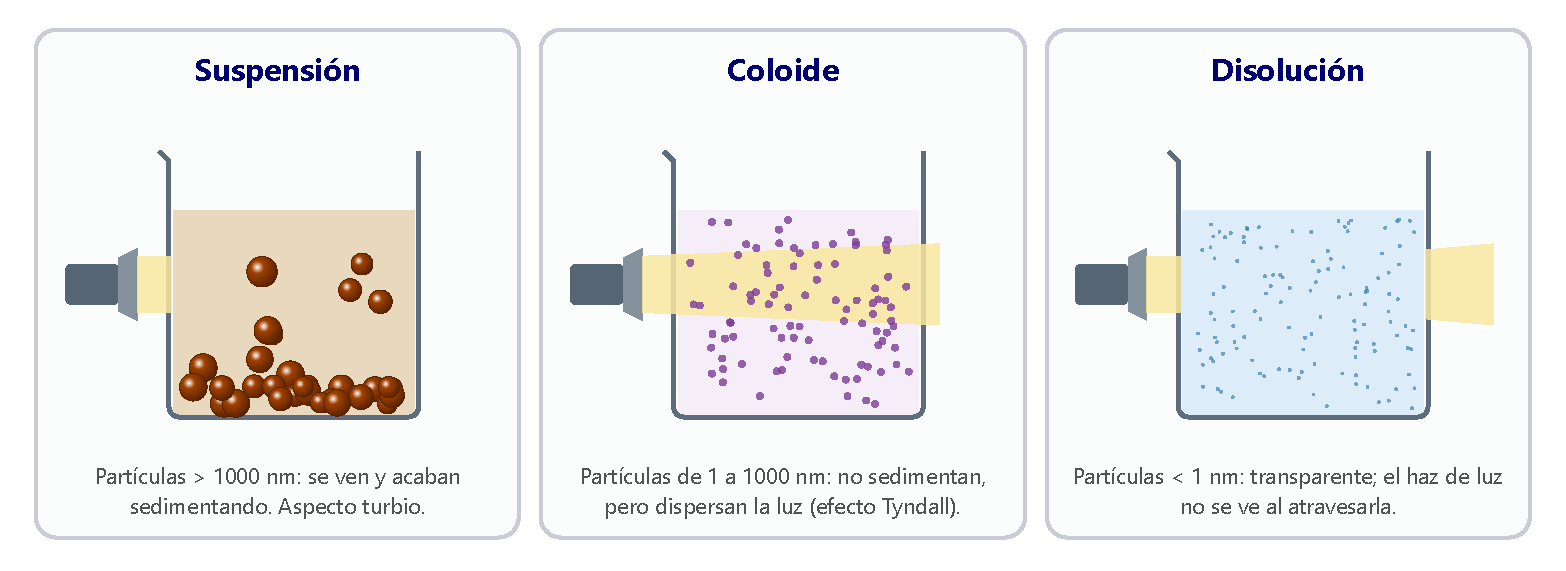
\includegraphics[width=0.95\textwidth]{images/UD2/tipos_mezclas}
    \caption{Un haz de luz permite distinguir un coloide de una disolución (efecto Tyndall).}
    \label{fig:ud2-tipos}
\end{figure}

Los coloides reciben nombres distintos según el estado de la fase dispersante y de la fase dispersa:

\begin{table}[H]
    \centering
    \caption{Tipos de coloides}
    \vspace{-5pt}
    \begin{tabular}{@{}lccc@{}}
        \toprule
        & \multicolumn{3}{c}{\textbf{Fase dispersa}} \\
        \cmidrule(l){2-4}
        \makecell{\textbf{Fase} \\ \textbf{dispersante}} & \textbf{Gas} & \textbf{Líquido} & \textbf{Sólido} \\
        \midrule
        Gas & \makecell{(siempre forman \\ disolución)} & \makecell{Aerosol líquido \\ (niebla, nubes)} & \makecell{Aerosol sólido \\ (humo, polvo)} \\[3pt]
        Líquido & \makecell{Espuma \\ (nata montada)} & \makecell{Emulsión \\ (leche, mayonesa)} & \makecell{Sol \\ (pinturas, tinta china)} \\[3pt]
        Sólido & \makecell{Espuma sólida \\ (piedra pómez)} & \makecell{Gel \\ (gelatina, queso)} & \makecell{Sol sólido \\ (vidrio de color)} \\
        \bottomrule
    \end{tabular}
    \label{tab:ud2-coloides}
\end{table}

\begin{exercise}
    Clasifica como mezcla heterogénea (suspensión), coloide o disolución: a) agua del grifo; b) niebla; c) zumo de naranja con
    pulpa; d) mayonesa; e) acero; f) arena con agua; g) gelatina; h) aire limpio.
    \begin{solu}
        \textcolor{red}{Disoluciones: a, e, h. Coloides: b (aerosol líquido), d (emulsión), g (gel). Heterogéneas: c y f
        (suspensiones).}
    \end{solu}
\end{exercise}

\begin{exercise}
    ¿Cómo distinguirías, con una linterna, un vaso de agua con un poco de leche de un vaso de agua con azúcar?
    \begin{solu}
        \textcolor{red}{Por el efecto Tyndall}: en el agua con leche (coloide) se ve el haz de luz al atravesarla; en el agua con
        azúcar (disolución) el haz no se ve.
    \end{solu}
\end{exercise}

%========================================================================================
\section{Características de las disoluciones}\label{sec:ud2-caracteristicas}
%========================================================================================

Una \textbf{disolución} es una mezcla homogénea: cualquier porción tiene la misma composición y las mismas propiedades. Sus
componentes son:

\begin{itemize}
    \item \textbf{Disolvente}: la fase dispersante. Suele ser el componente mayoritario y tiene el mismo estado de agregación que
    la disolución. Las \textbf{disoluciones acuosas}, en las que el disolvente es agua, son las más importantes: el agua disuelve
    tantas sustancias que se le llama \emph{disolvente universal}.
    \item \textbf{Soluto}: la fase dispersa, normalmente en menor proporción. Puede haber varios, y sus partículas disueltas pueden
    ser moléculas o iones.
\end{itemize}

\begin{table}[H]
    \centering
    \caption{Disoluciones según el estado de sus componentes}
    \vspace{-5pt}
    \begin{tabular}{@{}cccl@{}}
        \toprule
        \textbf{Disolvente} & \textbf{Soluto} & \textbf{Disolución} & \textbf{Ejemplo} \\
        \midrule
        Gas & Gas & Gas & Aire \\[3pt]
        Líquido & Gas & Líquido & Refresco con gas (\ch{CO2} en agua) \\[3pt]
        Líquido & Líquido & Líquido & Alcohol sanitario (etanol y agua) \\[3pt]
        Líquido & Sólido & Líquido & Agua de mar \\[3pt]
        Sólido & Gas & Sólido & Hidrógeno en paladio \\[3pt]
        Sólido & Líquido & Sólido & Amalgama de mercurio en plata \\[3pt]
        Sólido & Sólido & Sólido & Bronce (cobre y estaño) \\
        \bottomrule
    \end{tabular}
    \label{tab:ud2-tipos-disoluciones}
\end{table}

\subsection{El proceso de disolución}

Para que se forme una disolución, las partículas de soluto tienen que repartirse de manera uniforme entre las de disolvente. Esto
ocurre en tres pasos:
\begin{enumerate}
    \item Las partículas de soluto se separan entre sí, venciendo las fuerzas \textbf{soluto-soluto}.
    \item Las partículas de disolvente se separan, venciendo las fuerzas \textbf{disolvente-disolvente}.
    \item Las partículas de soluto y de disolvente se atraen (fuerzas \textbf{soluto-disolvente}). Cada partícula de soluto queda
    rodeada de moléculas de disolvente: es la \textbf{solvatación}, o \textbf{hidratación} si el disolvente es agua
    (figura~\ref{fig:ud2-nacl}).
\end{enumerate}

\begin{figure}[H]
    \centering
    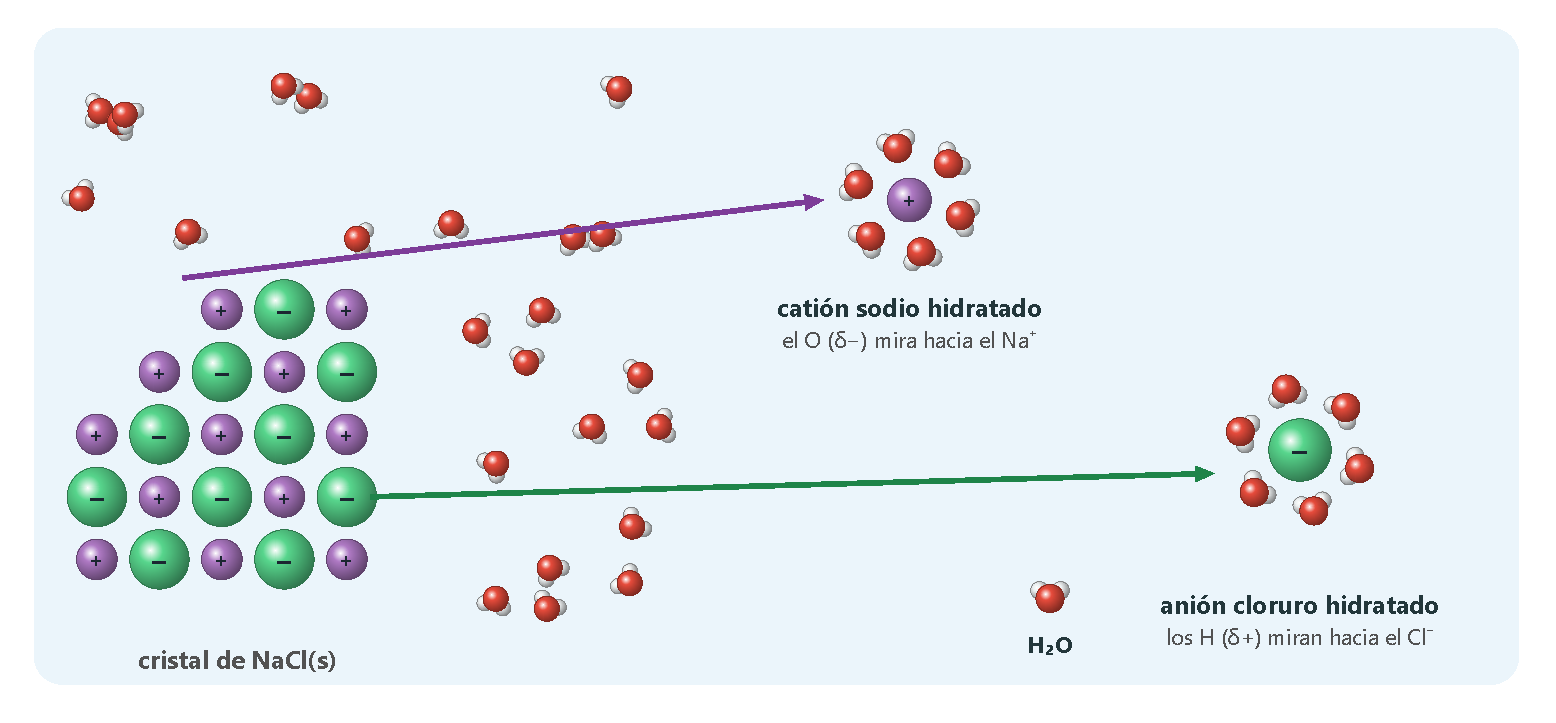
\includegraphics[width=0.9\textwidth]{images/UD2/disolucion_nacl}
    \caption{Disolución del cloruro de sodio: las moléculas de agua, polares, arrancan los iones del cristal y los rodean.}
    \label{fig:ud2-nacl}
\end{figure}

La sustancia se disuelve si las fuerzas soluto-disolvente son \textbf{más intensas} que las que hay que romper. Por eso, en
general, \textbf{«semejante disuelve a semejante»}: los solutos polares e iónicos se disuelven bien en disolventes polares (la sal
o el azúcar en agua), y los apolares, en disolventes apolares (el aceite no se disuelve en agua, pero sí en gasolina).

\paragraph{Factores que favorecen la disolución.} Todo lo que aumente el contacto entre soluto y disolvente acelera la
disolución de un sólido: que esté en \textbf{polvo} (más superficie de contacto), \textbf{agitar} (acerca disolvente nuevo a la
superficie del soluto) y \textbf{calentar} (las partículas se mueven más deprisa y se separan con más facilidad).

\begin{exercise}
    Explica por qué: a) el aceite no se disuelve en agua y sí en gasolina; b) un terrón de azúcar tarda más en disolverse que una
    cucharada de azúcar glas; c) el yodo, \ch{I2}, se disuelve mejor en tetracloruro de carbono que en agua.
    \begin{solu}
        a) \textcolor{red}{El aceite es apolar}: las fuerzas entre sus moléculas y las del agua (polar) son débiles; con la
        gasolina (apolar) sí son comparables. b) \textcolor{red}{El azúcar glas tiene mucha más superficie de contacto}. c)
        \textcolor{red}{El \ch{I2} y el \ch{CCl4} son apolares}: «semejante disuelve a semejante».
    \end{solu}
\end{exercise}

%========================================================================================
\section{Concentración de una disolución}\label{sec:ud2-concentracion}
%========================================================================================

La \textbf{concentración} relaciona la \textbf{cantidad de soluto} con la cantidad de disolución (o de disolvente). Es una
\textbf{propiedad intensiva}: no depende del tamaño de la muestra; un vaso y una cucharada de la misma disolución tienen la misma
concentración. Puede expresarse:

\begin{itemize}
    \item \textbf{Cualitativamente}: una disolución es \textbf{diluida} si tiene poco soluto, \textbf{concentrada} si tiene mucho y
    \textbf{saturada} si tiene el máximo posible.
    \item \textbf{Cuantitativamente}: con un número y su unidad. Las unidades se clasifican en \textbf{físicas}, que no tienen en
    cuenta la naturaleza del soluto, y \textbf{químicas}, que sí lo hacen (usan la cantidad de sustancia).
\end{itemize}

\subsection{Unidades físicas de concentración}

\begin{definition}[Porcentaje en masa]
    Gramos de soluto que hay en \qty{100}{\gram} de disolución:
    \[ \%\ \text{en masa} = \frac{m_{\text{soluto}}}{m_{\text{disolución}}} \cdot 100 \qquad (m_{\text{disolución}} = m_{\text{soluto}} + m_{\text{disolvente}}) \]
\end{definition}

\begin{definition}[Porcentaje en volumen]
    Volumen de soluto que hay en 100 unidades de volumen de disolución:
    \[ \%\ \text{en volumen} = \frac{V_{\text{soluto}}}{V_{\text{disolución}}} \cdot 100 \]
    En las bebidas alcohólicas se expresa en \textbf{grados}: \(1^{\circ}\) equivale al 1\,\% en volumen.
\end{definition}

\begin{definition}[Concentración en masa]
    Masa de soluto por unidad de volumen de disolución. Suele darse en \unit{\gram\per\litre} (en el SI, \unit{\kilo\gram\per\cubic\metre}):
    \[ \gamma = \frac{m_{\text{soluto}}}{V_{\text{disolución}}} \]
\end{definition}

\begin{remark}
    \textbf{¡Los volúmenes no son aditivos!} La masa de una disolución es siempre la suma de las masas de sus componentes, pero su
    volumen no: al mezclarse, las partículas se reacomodan y el volumen suele ser algo menor que la suma. Al mezclar \qty{50}{\mL}
    de etanol con \qty{50}{\mL} de agua se obtienen unos \qty{97}{\mL}. Por eso, salvo que el enunciado diga lo contrario, no se
    suman volúmenes.
\end{remark}

\paragraph{Concentración en masa y densidad.} Las dos se expresan, por ejemplo, en \unit{\gram\per\litre}, pero
\textbf{no miden lo mismo}:
\[ \gamma = \frac{m_{\text{soluto}}}{V_{\text{disolución}}} \qquad\qquad d = \frac{m_{\text{disolución}}}{V_{\text{disolución}}} = \frac{m_{\text{soluto}} + m_{\text{disolvente}}}{V_{\text{disolución}}} \]
La densidad de una sustancia pura es una propiedad característica; la de una disolución, no, porque depende de su concentración
(un huevo flota en agua muy salada y se hunde en agua dulce). La densidad sirve para pasar de masa de disolución a volumen de
disolución.

\paragraph{Partes por millón.} Para concentraciones muy pequeñas se usan las \textbf{partes por millón} (\unit{\ppm}): unidades
de soluto por cada millón de unidades de disolución, en masa o en volumen. En disoluciones acuosas diluidas,
\(\qty{1}{\ppm} \approx \qty{1}{\milli\gram\per\litre}\). Por ejemplo, más de \qty{50}{\ppm} en volumen de monóxido de carbono
en el aire es peligroso para la salud.

\begin{example}
    \textbf{Chocolate y vino.} a) Una tableta de \qty{200}{\gram} indica «70\,\% de cacao». ¿Cuánto cacao contiene?
    b) ¿Cuánto etanol hay en una botella de \qty{750}{\mL} de vino de \ang{13}?

    \textbf{Solución.} a) \(m_{\text{cacao}} = \qty{200}{\gram} \cdot \dfrac{\qty{70}{\gram}\ \text{cacao}}{\qty{100}{\gram}\ \text{tableta}} = \qty{140}{\gram}\) de cacao.

    b) \ang{13} significa 13\,\% en volumen: \(V_{\text{etanol}} = \qty{750}{\mL} \cdot \dfrac{13}{100} = \qty{97.5}{\mL}\) de etanol.
\end{example}

\begin{example}
    \textbf{Concentración en masa.} Se disuelven \qty{30}{\gram} de hidróxido de sodio en agua hasta tener \qty{250}{\mL} de
    disolución. Calcula su concentración en \unit{\gram\per\litre}.

    \textbf{Solución.} \(\gamma = \dfrac{\qty{30}{\gram}}{\qty{250}{\mL}} \cdot \dfrac{\qty{1000}{\mL}}{\qty{1}{\litre}} =
    \qty{120}{\gram\per\litre}\): cada litro de disolución contiene \qty{120}{\gram} de \ch{NaOH}.
\end{example}

\begin{exercise}
    Calcula el porcentaje en masa de una disolución preparada disolviendo \qty{12}{\gram} de cloruro de hidrógeno en
    \qty{140}{\gram} de agua.
    \begin{solu}
        \(\% = \dfrac{12}{12 + 140} \cdot 100 = \textcolor{red}{\qty{7.9}{\percent}}\).
    \end{solu}
\end{exercise}

\begin{exercise}
    Se mezclan \qty{250}{\gram} de sulfato de cobre(II) con \qty{1}{\litre} de agua (\(d = \qty{1}{\gram\per\mL}\)). ¿Cuál es el
    porcentaje en masa de la disolución?
    \begin{solu}
        \(m_{\text{agua}} = \qty{1000}{\gram}\): \(\% = \dfrac{250}{1250} \cdot 100 = \textcolor{red}{\qty{20}{\percent}}\).
    \end{solu}
\end{exercise}

\begin{exercise}
    Tenemos una disolución de ácido clorhídrico al 36\,\% en masa. a) ¿Qué masa de \ch{HCl} hay en \qty{400}{\gram} de disolución?
    b) ¿Qué masa de disolución contiene \qty{90}{\gram} de \ch{HCl}?
    \begin{solu}
        a) \(400 \cdot \dfrac{36}{100} = \textcolor{red}{\qty{144}{\gram}}\). b) \(90 \cdot \dfrac{100}{36} = \textcolor{red}{\qty{250}{\gram}}\) de disolución.
    \end{solu}
\end{exercise}

\begin{exercise}
    Se prepara una disolución de éter en cloroformo mezclando \qty{30}{\mL} de éter con \qty{150}{\mL} de cloroformo. Suponiendo
    los volúmenes aditivos, ¿cuál es su porcentaje en volumen?
    \begin{solu}
        \(\% = \dfrac{30}{30 + 150} \cdot 100 = \textcolor{red}{\qty{16.7}{\percent}}\) en volumen.
    \end{solu}
\end{exercise}

\begin{exercise}
    a) Calcula la concentración en \unit{\gram\per\litre} de una disolución con \qty{255}{\gram} de sulfato de cobre(II) en
    \qty{3}{\litre} de disolución. b) ¿Cuántos gramos de ácido nítrico hacen falta para preparar \qty{2.5}{\litre} de disolución
    de \qty{0.8}{\gram\per\litre}?
    \begin{solu}
        a) \(\gamma = 255/3 = \textcolor{red}{\qty{85}{\gram\per\litre}}\). b) \(m = \num{0.8} \cdot \num{2.5} = \textcolor{red}{\qty{2}{\gram}}\).
    \end{solu}
\end{exercise}

\begin{exercise}
    Una disolución acuosa de cloruro de sodio tiene una densidad de \qty{1.2}{\gram\per\cubic\cm} y una concentración de
    \qty{240}{\gram\per\litre}. a) ¿Cuál es la masa de \qty{150}{\mL} de disolución? b) ¿Cuánto \ch{NaCl} hay en
    \qty{250}{\mL}?
    \begin{solu}
        a) Con la densidad: \(m = \num{1.2} \cdot 150 = \textcolor{red}{\qty{180}{\gram}}\). b) Con la concentración:
        \(m = 240 \cdot \num{0.250} = \textcolor{red}{\qty{60}{\gram}}\) de \ch{NaCl}.
    \end{solu}
\end{exercise}

\begin{exercise}
    \label{ej:ud2-etanol}
    Se mezclan \qty{40}{\mL} de etanol (\(d = \qty{0.79}{\gram\per\mL}\)) con \qty{960}{\mL} de agua
    (\(d = \qty{1}{\gram\per\mL}\)) y se obtienen \qty{985}{\mL} de disolución. Expresa su concentración en \% en volumen,
    \unit{\gram\per\litre} y \% en masa.
    \begin{solu}
        \textcolor{blue}{\(m_{\text{etanol}} = 40 \cdot \num{0.79} = \qty{31.6}{\gram}\); \(m_{\text{agua}} = \qty{960}{\gram}\).}
        \% vol \(= 40/985 \cdot 100 = \textcolor{red}{\qty{4.06}{\percent}}\);
        \(\gamma = \num{31.6}/\num{0.985} = \textcolor{red}{\qty{32.1}{\gram\per\litre}}\);
        \% masa \(= \num{31.6}/\num{991.6} \cdot 100 = \textcolor{red}{\qty{3.19}{\percent}}\).
    \end{solu}
\end{exercise}

\begin{exercise}
    Un litro de leche semidesnatada contiene \qty{48}{\gram} de lactosa y tiene una densidad de \qty{1.03}{\gram\per\cubic\cm}.
    Calcula: a) el porcentaje en masa de lactosa; b) su concentración en \unit{\gram\per\litre}; c) la lactosa que hay en un vaso
    de \qty{150}{\mL}.
    \begin{solu}
        a) \(m_{\text{leche}} = \qty{1030}{\gram}\): \(\% = 48/1030 \cdot 100 = \textcolor{red}{\qty{4.66}{\percent}}\).
        b) \(\textcolor{red}{\qty{48}{\gram\per\litre}}\). c) \(48 \cdot \num{0.150} = \textcolor{red}{\qty{7.2}{\gram}}\).
    \end{solu}
\end{exercise}

\begin{exercise}
    En \qty{300}{\mL} de una disolución de glucosa hay \qty{15}{\gram} de soluto. Su densidad es \qty{1.02}{\gram\per\cubic\cm}.
    a) Calcula su concentración en \% en masa y en \unit{\gram\per\litre}. b) Si un niño puede tomar como mucho \qty{20}{\gram}
    de glucosa, ¿qué volumen de disolución podrá tomar como máximo?
    \begin{solu}
        a) \(m_{\text{disolución}} = 300 \cdot \num{1.02} = \qty{306}{\gram}\): \(\% = 15/306 \cdot 100 = \textcolor{red}{\qty{4.9}{\percent}}\);
        \(\gamma = 15/\num{0.3} = \textcolor{red}{\qty{50}{\gram\per\litre}}\). b) \(V = 20/50 = \qty{0.4}{\litre} = \textcolor{red}{\qty{400}{\mL}}\).
    \end{solu}
\end{exercise}

\subsection{Unidades químicas de concentración}

Tienen en cuenta la naturaleza del soluto, porque utilizan su \textbf{cantidad de sustancia} (los moles), que se calcula con la
masa molar: \(n = m/M\). Solo las sustancias puras tienen masa molar; por eso hay que calcular por separado los moles de cada
componente.

\begin{definition}[Concentración molar o molaridad]
    Moles de soluto por litro de disolución. Su unidad es el \unit{\mol\per\litre}, que se abrevia \unit{\M} («molar»):
    \[ c = \frac{n_{\text{soluto}}}{V_{\text{disolución}}\ (\unit{\litre})} \]
\end{definition}

\begin{definition}[Molalidad]
    Moles de soluto por kilogramo de \textbf{disolvente}. Su unidad es el \unit{\mol\per\kilo\gram}:
    \[ m = \frac{n_{\text{soluto}}}{m_{\text{disolvente}}\ (\unit{\kilo\gram})} \]
\end{definition}

\begin{definition}[Fracción molar]
    Moles de un componente \(i\) entre los moles totales de la disolución. No tiene unidades, y la suma de las fracciones molares
    de todos los componentes vale 1:
    \[ \chi_i = \frac{n_i}{n_{\text{total}}} \qquad\qquad \chi_{\text{soluto}} + \chi_{\text{disolvente}} = 1 \]
\end{definition}

\begin{remark}
    La molalidad es la única concentración que se refiere al disolvente y no a la disolución. Como no depende del volumen, no cambia
    con la temperatura, y por eso se usa en las propiedades coligativas. ¡Cuidado con los símbolos!: \(m\) (molalidad) y
    \(M\) (masa molar) también se usan para la masa; fíjate siempre en las unidades.
\end{remark}

\begin{table}[H]
    \centering
    \caption{Resumen de las unidades de concentración}
    \vspace{-5pt}
    \begin{tabular}{@{}lcc@{}}
        \toprule
        \textbf{Unidad} & \textbf{Expresión} & \textbf{Unidad habitual} \\
        \midrule
        Porcentaje en masa & \(\dfrac{m_{\text{soluto}}}{m_{\text{disolución}}} \cdot 100\) & \% \\[9pt]
        Porcentaje en volumen & \(\dfrac{V_{\text{soluto}}}{V_{\text{disolución}}} \cdot 100\) & \% (grados) \\[9pt]
        Concentración en masa & \(\dfrac{m_{\text{soluto}}}{V_{\text{disolución}}}\) & \unit{\gram\per\litre} \\[9pt]
        Concentración molar & \(\dfrac{n_{\text{soluto}}}{V_{\text{disolución}}}\) & \unit{\mol\per\litre} (\unit{\M}) \\[9pt]
        Molalidad & \(\dfrac{n_{\text{soluto}}}{m_{\text{disolvente}}}\) & \unit{\mol\per\kilo\gram} \\[9pt]
        Fracción molar & \(\dfrac{n_i}{n_{\text{total}}}\) & sin unidades \\
        \bottomrule
    \end{tabular}
    \label{tab:ud2-unidades}
\end{table}

\begin{example}
    \textbf{Molaridad y molalidad de una disolución de glucosa.} Se disuelven \qty{45}{\gram} de glucosa, \ch{C6H12O6}, en agua
    hasta obtener \qty{2}{\litre} de disolución, de densidad \qty{1.02}{\gram\per\cubic\cm}. Calcula: a) la concentración molar;
    b) la molalidad.

    \textbf{Solución.} \(M(\ch{C6H12O6}) = 6 \cdot 12 + 12 \cdot 1 + 6 \cdot 16 = \qty{180}{\gram\per\mol}\);
    \(n = \dfrac{45}{180} = \qty{0.25}{\mol}\).

    a) \(c = \dfrac{\qty{0.25}{\mol}}{\qty{2}{\litre}} = \qty{0.125}{\mol\per\litre}\).

    b) Con la densidad hallamos la masa de disolución y, restando el soluto, la del disolvente:
    \(m_{\text{disolución}} = \qty{2000}{\mL} \cdot \qty{1.02}{\gram\per\mL} = \qty{2040}{\gram}\);
    \(m_{\text{agua}} = 2040 - 45 = \qty{1995}{\gram}\).
    \[ m = \frac{\qty{0.25}{\mol}}{\qty{1.995}{\kilo\gram}} = \qty{0.125}{\mol\per\kilo\gram} \]
    En disoluciones acuosas diluidas, molaridad y molalidad casi coinciden.
\end{example}

\begin{example}
    \textbf{Fracción molar.} a) Un recipiente contiene \qty{280}{\gram} de nitrógeno y \qty{50}{\gram} de hidrógeno. Calcula la
    fracción molar de cada gas. b) Se disuelven \qty{46}{\gram} de etanol, \ch{C2H6O}, en \qty{500}{\gram} de agua. Calcula la
    fracción molar del etanol y la molalidad.

    \textbf{Solución.} a) \(n(\ch{N2}) = 280/28 = \qty{10}{\mol}\); \(n(\ch{H2}) = 50/2 = \qty{25}{\mol}\).
    \(\chi(\ch{N2}) = \dfrac{10}{35} = \num{0.286}\); \(\chi(\ch{H2}) = \dfrac{25}{35} = \num{0.714}\). Comprobamos que suman 1.

    b) \(n_{\text{etanol}} = 46/46 = \qty{1}{\mol}\); \(n_{\text{agua}} = 500/18 = \qty{27.8}{\mol}\).
    \(\chi_{\text{etanol}} = \dfrac{1}{1 + \num{27.8}} = \num{0.035}\); \(m = \dfrac{\qty{1}{\mol}}{\qty{0.5}{\kilo\gram}} = \qty{2}{\mol\per\kilo\gram}\).
\end{example}

\begin{example}
    \label{ex:ud2-sulfurico}
    \textbf{Una botella de ácido sulfúrico.} La etiqueta de una botella de ácido sulfúrico indica: «95\,\% de riqueza en masa;
    \(d = \qty{1.83}{\gram\per\cubic\cm}\)». Calcula su concentración en \unit{\gram\per\litre}, su concentración molar y su
    molalidad.

    \textbf{Solución.} \(M(\ch{H2SO4}) = \qty{98}{\gram\per\mol}\). Encadenamos factores de conversión partiendo de la riqueza
    (\qty{95}{\gram} de ácido por cada \qty{100}{\gram} de disolución):
    \[ \gamma = \frac{\qty{95}{\gram}\ \ch{H2SO4}}{\qty{100}{\gram}\ \text{dis.}} \cdot \frac{\qty{1.83}{\gram}\ \text{dis.}}{\qty{1}{\cubic\cm}} \cdot
    \frac{\qty{1000}{\cubic\cm}}{\qty{1}{\litre}} = \qty{1738.5}{\gram\per\litre} \]
    \[ c = \frac{\qty{1738.5}{\gram}\ \ch{H2SO4}}{\qty{1}{\litre}} \cdot \frac{\qty{1}{\mol}}{\qty{98}{\gram}} = \qty{17.7}{\mol\per\litre} \]
    Para la molalidad, en \qty{100}{\gram} de disolución hay \qty{95}{\gram} de ácido y \(100 - 95 = \qty{5}{\gram}\) de agua:
    \[ m = \frac{95/98\ \unit{\mol}}{\qty{0.005}{\kilo\gram}} = \qty{194}{\mol\per\kilo\gram} \]
\end{example}

\begin{exercise}
    ¿Qué masa de cloruro de calcio, \ch{CaCl2}, hay que disolver para obtener \qty{200}{\mL} de disolución
    \qty{0.15}{\mol\per\litre}?
    \begin{solu}
        \(n = \num{0.15} \cdot \num{0.2} = \qty{0.03}{\mol}\); \(M = \qty{111}{\gram\per\mol}\): \(m = \textcolor{red}{\qty{3.33}{\gram}}\).
    \end{solu}
\end{exercise}

\begin{exercise}
    ¿Cuántos gramos de \ch{FeCl2} hay en \qty{80}{\gram} de una disolución acuosa \qty{0.2}{\mol\per\kilo\gram}?
    \begin{solu}
        \textcolor{blue}{\(M = \qty{126.8}{\gram\per\mol}\). Por cada kg de agua hay \qty{0.2}{\mol} (\qty{25.36}{\gram}) de soluto,
        es decir, \qty{1025.36}{\gram} de disolución.} \(m = 80 \cdot \dfrac{\num{25.36}}{\num{1025.36}} = \textcolor{red}{\qty{1.98}{\gram}}\).
    \end{solu}
\end{exercise}

\begin{exercise}
    ¿Qué volumen de una disolución de maltosa, \ch{C12H22O11}, \qty{4}{\mol\per\litre} contiene \qty{150}{\gram} de maltosa?
    \begin{solu}
        \(M = \qty{342}{\gram\per\mol}\); \(n = 150/342 = \qty{0.439}{\mol}\): \(V = \num{0.439}/4 = \qty{0.110}{\litre} = \textcolor{red}{\qty{110}{\mL}}\).
    \end{solu}
\end{exercise}

\begin{exercise}
    Una mezcla contiene \qty{40}{\gram} de metanol, \ch{CH3OH}, y \qty{90}{\gram} de agua. Calcula la fracción molar de cada
    componente.
    \begin{solu}
        \(n_{\text{metanol}} = 40/32 = \qty{1.25}{\mol}\); \(n_{\text{agua}} = 90/18 = \qty{5}{\mol}\):
        \(\chi_{\text{metanol}} = \textcolor{red}{\num{0.2}}\); \(\chi_{\text{agua}} = \textcolor{red}{\num{0.8}}\).
    \end{solu}
\end{exercise}

\begin{exercise}
    Calcula la concentración en \unit{\gram\per\litre}, la concentración molar y la molalidad de un ácido clorhídrico comercial
    del 35\,\% en masa y densidad \qty{1.18}{\gram\per\mL}.
    \begin{solu}
        \(\gamma = \num{0.35} \cdot 1180 = \textcolor{red}{\qty{413}{\gram\per\litre}}\); \(c = 413/\num{36.5} = \textcolor{red}{\qty{11.3}{\mol\per\litre}}\);
        \(m = \dfrac{35/\num{36.5}}{\num{0.065}} = \textcolor{red}{\qty{14.8}{\mol\per\kilo\gram}}\).
    \end{solu}
\end{exercise}

\begin{exercise}
    Repite el ejercicio anterior para un ácido nítrico comercial del 65\,\% en masa y densidad \qty{1.40}{\gram\per\mL}.
    \begin{solu}
        \(\gamma = \textcolor{red}{\qty{910}{\gram\per\litre}}\); \(c = 910/63 = \textcolor{red}{\qty{14.4}{\mol\per\litre}}\);
        \(m = \dfrac{65/63}{\num{0.035}} = \textcolor{red}{\qty{29.5}{\mol\per\kilo\gram}}\).
    \end{solu}
\end{exercise}

%========================================================================================
\section{Preparación de una disolución}\label{sec:ud2-preparacion}
%========================================================================================

Preparar disoluciones de concentración conocida es una tarea habitual en un laboratorio, pero también en una farmacia, un
hospital o una industria alimentaria. Veremos cómo preparar una disolución líquida a partir de un \textbf{soluto sólido} y a
partir de \textbf{otra disolución} más concentrada. En el laboratorio, recuerda: protege ojos y manos, usa cada instrumento como
corresponde y mide masas y volúmenes con cuidado.

\subsection{A partir de un soluto sólido}

Primero se \textbf{calcula} la masa de soluto necesaria. Después (figura~\ref{fig:ud2-prep-solido}):
\begin{enumerate}[label=\numberballgreen]
    \item Se coloca un vidrio de reloj en la balanza, se pulsa «tara» y se \textbf{pesa} el soluto con una espátula.
    \item Se \textbf{disuelve} en un vaso de precipitados con un poco de agua destilada (menos del volumen final), agitando con una
    varilla.
    \item Se \textbf{trasvasa} a un matraz aforado del volumen deseado con ayuda de un embudo. Se enjuaga el vaso con un poco de
    agua y se añade también al matraz, para no perder soluto.
    \item Se añade agua destilada hasta cerca de la marca y se termina con un cuentagotas: se \textbf{enrasa} cuando la parte
    inferior del menisco toca la marca de aforo, mirando a la altura de los ojos.
    \item Se tapa, se agita para homogeneizar y se \textbf{etiqueta} con la fórmula del soluto, la concentración y la fecha.
\end{enumerate}

\begin{figure}[H]
    \centering
    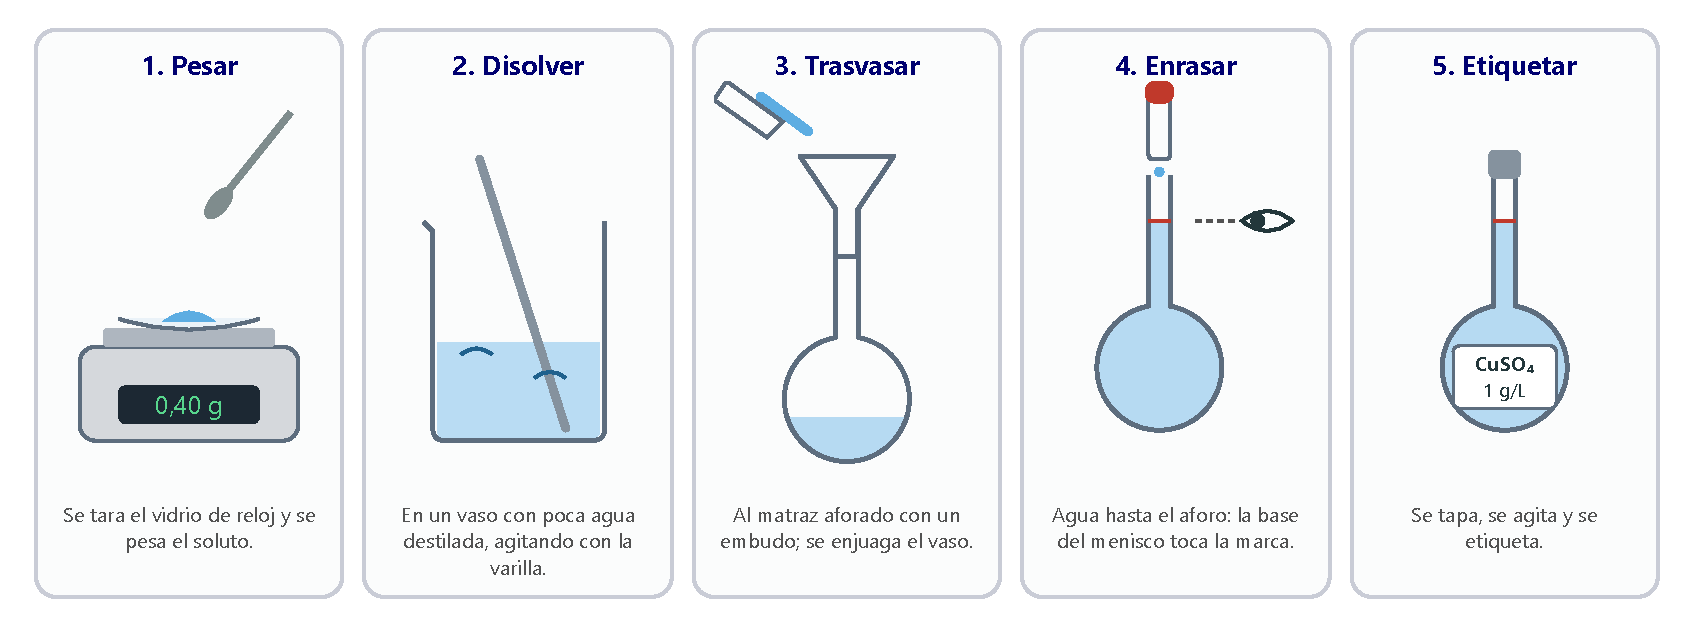
\includegraphics[width=\textwidth]{images/UD2/preparacion_solido}
    \caption{Pasos para preparar una disolución a partir de un soluto sólido.}
    \label{fig:ud2-prep-solido}
\end{figure}

\begin{example}
    \textbf{Disolución de sulfato de cobre(II).} ¿Cómo prepararías \qty{250}{\mL} de una disolución de \ch{CuSO4}
    \qty{0.1}{\mol\per\litre}?

    \textbf{Solución.} \(M(\ch{CuSO4}) = \num{63.5} + 32 + 4 \cdot 16 = \qty{159.5}{\gram\per\mol}\).
    \[ \qty{0.250}{\litre} \cdot \frac{\qty{0.1}{\mol}}{\qty{1}{\litre}} \cdot \frac{\qty{159.5}{\gram}}{\qty{1}{\mol}} = \qty{3.99}{\gram} \]
    Se pesan \qty{3.99}{\gram} de \ch{CuSO4}, se disuelven en un vaso con unos \qty{100}{\mL} de agua destilada, se pasan a un
    matraz aforado de \qty{250}{\mL} y se enrasa.
\end{example}

\subsection{A partir de otra disolución: dilución}

\textbf{Diluir} es añadir disolvente a una disolución para obtener otra de \textbf{menor} concentración. La clave es que, al
añadir disolvente, \textbf{los moles de soluto no cambian}: los que tomamos de la disolución concentrada (\(c_1\), \(V_1\)) son
los que habrá en la diluida (\(c_2\), \(V_2\)):
\[ n = c_1 V_1 = c_2 V_2 \]
Con una \textbf{pipeta} se toma el volumen \(V_1\) de la disolución concentrada, se vierte en un matraz aforado de volumen \(V_2\)
que ya contenga algo de agua destilada y se enrasa (figura~\ref{fig:ud2-dilucion}).

\begin{figure}[H]
    \centering
    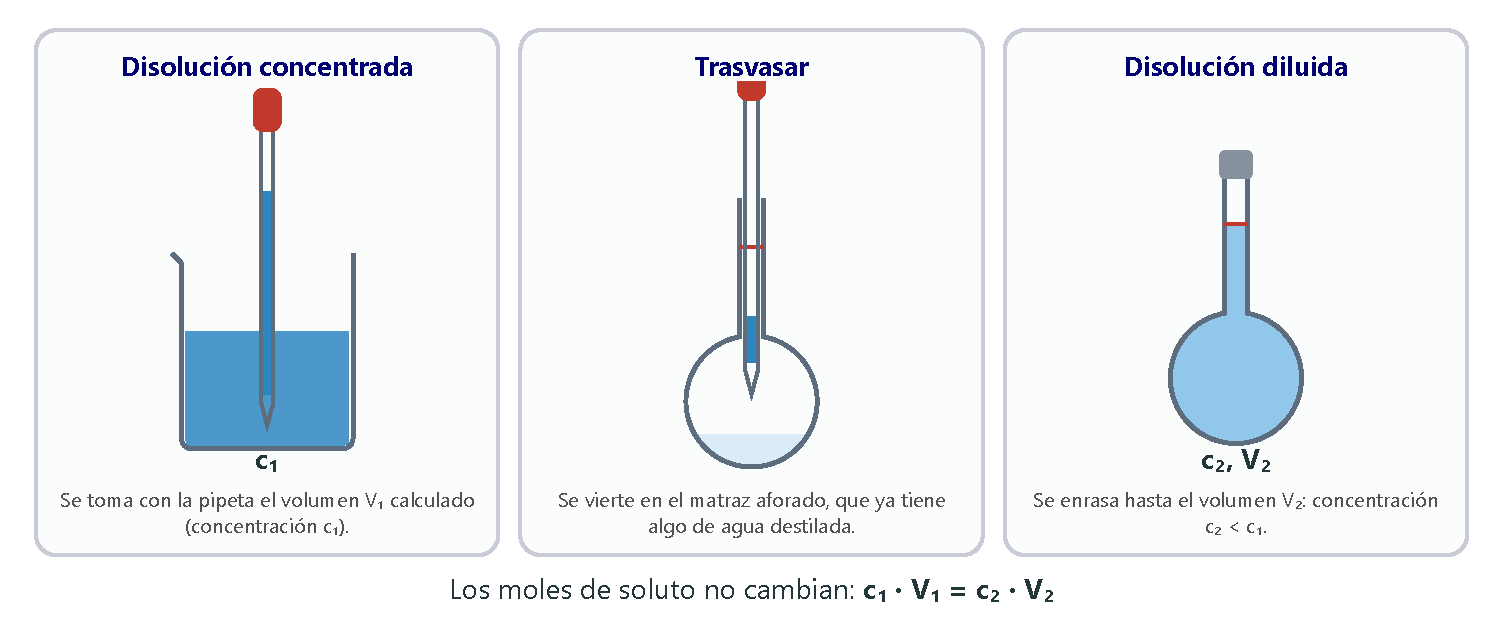
\includegraphics[width=0.85\textwidth]{images/UD2/dilucion}
    \caption{Preparación de una disolución diluida a partir de otra concentrada.}
    \label{fig:ud2-dilucion}
\end{figure}

\begin{remark}
    \textbf{Seguridad: el ácido sobre el agua.} Al diluir ácidos concentrados (sobre todo el sulfúrico) se desprende mucho calor.
    Por eso se vierte siempre \textbf{el ácido sobre el agua}, poco a poco, y nunca al revés: el agua añadida sobre el ácido podría
    hervir de golpe y salpicar.
\end{remark}

\begin{example}
    \textbf{Ácido nítrico diluido a partir del comercial.} Hay que preparar \qty{250}{\mL} de ácido nítrico
    \qty{0.4}{\mol\per\litre} a partir de un ácido comercial del 65\,\% en masa y densidad \qty{1.40}{\gram\per\mL}. ¿Qué
    volumen del comercial se necesita?

    \textbf{Solución.} 1) Moles de \ch{HNO3} necesarios: \(n = \num{0.4} \cdot \num{0.250} = \qty{0.1}{\mol}\).

    2) Volumen de ácido comercial que los contiene, encadenando masa molar, riqueza y densidad:
    \[ \qty{0.1}{\mol} \cdot \frac{\qty{63}{\gram}\ \ch{HNO3}}{\qty{1}{\mol}} \cdot \frac{\qty{100}{\gram}\ \text{dis.}}{\qty{65}{\gram}\ \ch{HNO3}} \cdot
    \frac{\qty{1}{\mL}}{\qty{1.40}{\gram}\ \text{dis.}} = \qty{6.9}{\mL} \]
    3) Con una pipeta se toman \qty{6.9}{\mL} del ácido comercial, se vierten en un matraz aforado de \qty{250}{\mL} con unos
    \qty{100}{\mL} de agua destilada, se enrasa, se tapa, se agita y se etiqueta.
\end{example}

\begin{example}
    \textbf{Dilución y mezcla.} a) ¿Qué volumen final debe tener una disolución que se prepara añadiendo agua a \qty{400}{\mL} de
    otra \qty{0.6}{\mol\per\litre} para que su concentración sea \qty{0.25}{\mol\per\litre}? b) Se mezclan \qty{200}{\mL} de
    \ch{NaCl} \qty{0.5}{\mol\per\litre} con \qty{300}{\mL} de \ch{NaCl} \qty{1}{\mol\per\litre}. Suponiendo volúmenes aditivos,
    ¿cuál es la concentración de la mezcla?

    \textbf{Solución.} a) \(V_2 = \dfrac{c_1 V_1}{c_2} = \dfrac{\num{0.6} \cdot \num{0.4}}{\num{0.25}} = \qty{0.96}{\litre}\):
    hay que añadir \(960 - 400 = \qty{560}{\mL}\) de agua.

    b) Se suman los moles de soluto y los volúmenes:
    \(n = \num{0.5} \cdot \num{0.2} + 1 \cdot \num{0.3} = \qty{0.4}{\mol}\); \(c = \dfrac{\num{0.4}}{\num{0.5}} = \qty{0.8}{\mol\per\litre}\).
\end{example}

\begin{exercise}
    Tenemos \qty{200}{\mL} de ácido clorhídrico \qty{2}{\mol\per\litre} y añadimos agua hasta que la concentración se reduce a la
    tercera parte. ¿Cuál es el volumen final?
    \begin{solu}
        \(V_2 = \dfrac{2 \cdot \num{0.2}}{2/3} = \textcolor{red}{\qty{0.6}{\litre}}\).
    \end{solu}
\end{exercise}

\begin{exercise}
    Se añaden \qty{1.5}{\litre} de agua a \qty{300}{\mL} de ácido nítrico \qty{4}{\mol\per\litre}. Suponiendo volúmenes aditivos,
    calcula la concentración final.
    \begin{solu}
        \(c_2 = \dfrac{4 \cdot \num{0.3}}{\num{1.8}} = \textcolor{red}{\qty{0.67}{\mol\per\litre}}\).
    \end{solu}
\end{exercise}

\begin{exercise}
    ¿Cómo podrías aumentar la concentración de una disolución de etanol \qty{0.5}{\mol\per\litre}?
    \begin{solu}
        \textcolor{red}{Añadiendo más etanol (soluto) o eliminando disolvente}; en este caso no sirve evaporar, porque el etanol es más
        volátil que el agua. También se puede mezclar con otra disolución más concentrada.
    \end{solu}
\end{exercise}

%========================================================================================
\section{Solubilidad}\label{sec:ud2-solubilidad}
%========================================================================================

Una sustancia puede ser soluble en un disolvente e insoluble en otro: el aceite se disuelve en acetona, pero no en agua. Y aunque
sea soluble, hay un \textbf{límite}: si echas azúcar en un vaso de agua y remueves, llega un momento en que ya no se disuelve más y
el exceso se queda en el fondo. Decimos entonces que la disolución está \textbf{saturada}, y que el soluto añadido
\textbf{precipita} (figura~\ref{fig:ud2-saturacion}).

\begin{definition}[Solubilidad]
    Cantidad máxima de soluto que se puede disolver en una cantidad determinada de disolvente a una presión y temperatura dadas. Es
    la concentración de la disolución saturada. Suele expresarse en gramos de soluto por \qty{100}{\gram} de disolvente o en
    \unit{\gram\per\litre}.
\end{definition}

\begin{figure}[H]
    \centering
    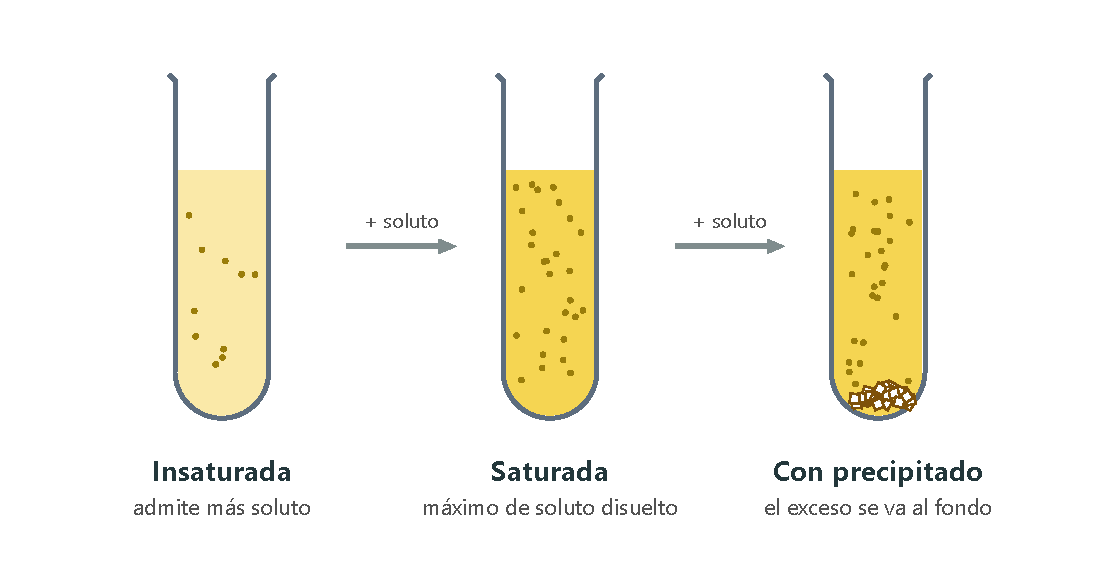
\includegraphics[width=0.6\textwidth]{images/UD2/saturacion}
    \caption{Al añadir soluto, una disolución pasa de insaturada a saturada; el soluto que sobra precipita.}
    \label{fig:ud2-saturacion}
\end{figure}

\subsection{Solubilidad y temperatura}

\paragraph{Sólidos en líquidos.} La \textbf{curva de solubilidad} representa la solubilidad de un soluto frente a la temperatura
(figura~\ref{fig:ud2-curvas}). En general, la solubilidad de los sólidos \textbf{aumenta} con la temperatura, aunque en algunos
casos apenas cambia (\ch{NaCl}) y en otros disminuye (\ch{Ce2(SO4)3}).

Si una disolución saturada en caliente se enfría, el soluto que ya no cabe precipita. El clorato de potasio, \ch{KClO3}, por
ejemplo, tiene una solubilidad de unos \qty{30}{\gram} en \qty{100}{\gram} de agua a \qty{70}{\degreeCelsius}, pero solo de
\qty{10}{\gram} a \qty{30}{\degreeCelsius}: al enfriar una disolución saturada que contenga \qty{100}{\gram} de agua, precipitan
unos \qty{20}{\gram} de \ch{KClO3}. Si el enfriamiento es muy lento y sin perturbaciones, puede que el exceso no precipite: se
obtiene una \textbf{disolución sobresaturada}, muy inestable; un golpe o un cristalito de soluto basta para que el exceso se separe,
a veces formando bonitos \textbf{cristales}.

\begin{figure}[H]
    \centering
    \begin{tikzpicture}
        \begin{axis}[grafica, width=0.7\linewidth, height=7.5cm,
            xlabel={Temperatura (\unit{\degreeCelsius})}, ylabel={Solubilidad (g / \qty{100}{\gram} de agua)},
            xmin=0, xmax=100, ymin=0, ymax=120, xtick={0,10,...,100}, ytick={0,20,...,120},
            clip=true, legend style={font=\scriptsize, at={(1.04,1)}, anchor=north west, cells={anchor=west}}]
            \addplot[thick, smooth, blue!70!black] coordinates {(0,13.3) (10,20.9) (20,31.6) (30,45.8) (40,63.9) (50,85.5) (60,110) (64,120)};
            \addplot[thick, smooth, green!50!black] coordinates {(0,59.5) (10,64.7) (20,74.5) (30,100) (40,116) (45,120)};
            \addplot[thick, smooth, orange!90!black] coordinates {(0,4.7) (10,7) (20,12) (30,20) (40,26) (50,34) (60,43) (70,52) (80,61) (90,70) (100,80)};
            \addplot[thick, smooth, red!70!black] coordinates {(0,28) (20,34.2) (40,40.1) (60,45.8) (80,51.3) (100,56.3)};
            \addplot[thick, smooth, violet] coordinates {(0,3.3) (10,5.2) (20,7.3) (30,10.1) (40,13.9) (50,19.3) (60,23.8) (70,30) (80,37.6) (90,46) (100,56.3)};
            \addplot[thick, smooth, black!70] coordinates {(0,35.7) (20,35.9) (40,36.4) (60,37.1) (80,38) (100,39.2)};
            \addplot[thick, smooth, brown!80!black] coordinates {(0,20) (10,15) (20,10) (30,7.2) (40,5.5) (60,3.8) (80,2.6) (100,2)};
            \legend{\ch{KNO3}, \ch{CaCl2}, \ch{K2Cr2O7}, \ch{KCl}, \ch{KClO3}, \ch{NaCl}, \ch{Ce2(SO4)3}}
        \end{axis}
    \end{tikzpicture}
    \caption{Curvas de solubilidad de algunas sales en agua (valores aproximados).}
    \label{fig:ud2-curvas}
\end{figure}

\paragraph{Gases en líquidos.} Cuando sacas un refresco de la nevera y lo sirves, se forman burbujas: al calentarse, el
\ch{CO2} disuelto escapa. La solubilidad de los \textbf{gases} en los líquidos \textbf{disminuye} al aumentar la temperatura
(figura~\ref{fig:ud2-gases}), porque las moléculas de gas, con más energía, escapan con más facilidad de la disolución.

\begin{figure}[H]
    \centering
    \begin{tikzpicture}
        \begin{axis}[grafica, width=0.48\linewidth, height=5cm,
            xlabel={\(t\) (\unit{\degreeCelsius})}, ylabel={\ch{CO2} disuelto (\unit{\gram\per\litre})},
            xmin=0, xmax=80, ymin=0, ymax=3.6, xtick={0,20,...,80}]
            \addplot[thick, smooth, red!75!black] coordinates {(0,3.35) (10,2.32) (20,1.69) (30,1.26) (40,0.97) (50,0.76) (60,0.58) (80,0.30)};
        \end{axis}
    \end{tikzpicture}
    \hfill
    \begin{tikzpicture}
        \begin{axis}[grafica, width=0.48\linewidth, height=5cm,
            xlabel={\(t\) (\unit{\degreeCelsius})}, ylabel={\ch{O2} disuelto (\unit{\milli\gram\per\litre})},
            xmin=0, xmax=40, ymin=0, ymax=16, xtick={0,10,...,40}]
            \addplot[thick, smooth, blue!70!black] coordinates {(0,14.6) (5,12.8) (10,11.3) (15,10.1) (20,9.1) (25,8.3) (30,7.6) (35,7.0) (40,6.4)};
        \end{axis}
    \end{tikzpicture}
    \caption{Solubilidad del dióxido de carbono (a \qty{1}{\atm} de \ch{CO2}) y del oxígeno (en contacto con el aire) en agua.}
    \label{fig:ud2-gases}
\end{figure}

\begin{example}
    \textbf{Lectura de las curvas de solubilidad.} Con la figura~\ref{fig:ud2-curvas}: a) compara la solubilidad del
    \ch{K2Cr2O7} a 20, 60 y \qty{80}{\degreeCelsius}; b) ¿qué es más soluble a \qty{20}{\degreeCelsius}, el \ch{CaCl2} o el
    \ch{KCl}? c) Se enfría hasta \qty{30}{\degreeCelsius} una disolución saturada de \ch{KClO3} a \qty{70}{\degreeCelsius} que
    contiene \qty{250}{\gram} de agua. ¿Cuánto soluto precipita?

    \textbf{Solución.} a) Unos \qty{12}{\gram}, \qty{43}{\gram} y \qty{61}{\gram} por \qty{100}{\gram} de agua: aumenta mucho
    con la temperatura, como en la mayoría de las sales. b) El \ch{CaCl2}: unos \qty{75}{\gram} frente a unos \qty{34}{\gram} de
    \ch{KCl}. c) En \qty{100}{\gram} de agua precipitan \(30 - 10 = \qty{20}{\gram}\); en \qty{250}{\gram},
    \(20 \cdot \num{2.5} = \qty{50}{\gram}\) de \ch{KClO3}.
\end{example}

\begin{example}
    \textbf{Vertidos de agua caliente.} Una empresa vierte agua caliente a un río. ¿Cómo afecta a los peces?

    \textbf{Solución.} Los peces respiran el oxígeno disuelto en el agua. Al aumentar la temperatura disminuye la solubilidad del
    oxígeno (figura~\ref{fig:ud2-gases}): a \qty{30}{\degreeCelsius} el agua disuelve casi la mitad que a \qty{0}{\degreeCelsius}.
    Esta \textbf{contaminación térmica} deja menos oxígeno disponible, y los peces pueden morir asfixiados.
\end{example}

\subsection{Solubilidad de los gases y presión}

La presión apenas influye en la solubilidad de sólidos y líquidos, pero mucho en la de los gases. Las moléculas de un gas chocan
contra la superficie del líquido; si la presión aumenta, hay más choques y se disuelven más moléculas hasta alcanzar un nuevo
equilibrio (figura~\ref{fig:ud2-henry}). \textbf{William Henry} (1775-1836) recogió este comportamiento en una ley:

\begin{definition}[Ley de Henry]
    A temperatura constante, la solubilidad de un gas en un líquido es directamente proporcional a la presión parcial del gas
    sobre la disolución:
    \[ c = k \, p \]
    La constante \(k\) depende del gas, del disolvente y de la temperatura (por ejemplo, en \unit{\mol\per\litre\per\atm}).
\end{definition}

\begin{figure}[H]
    \centering
    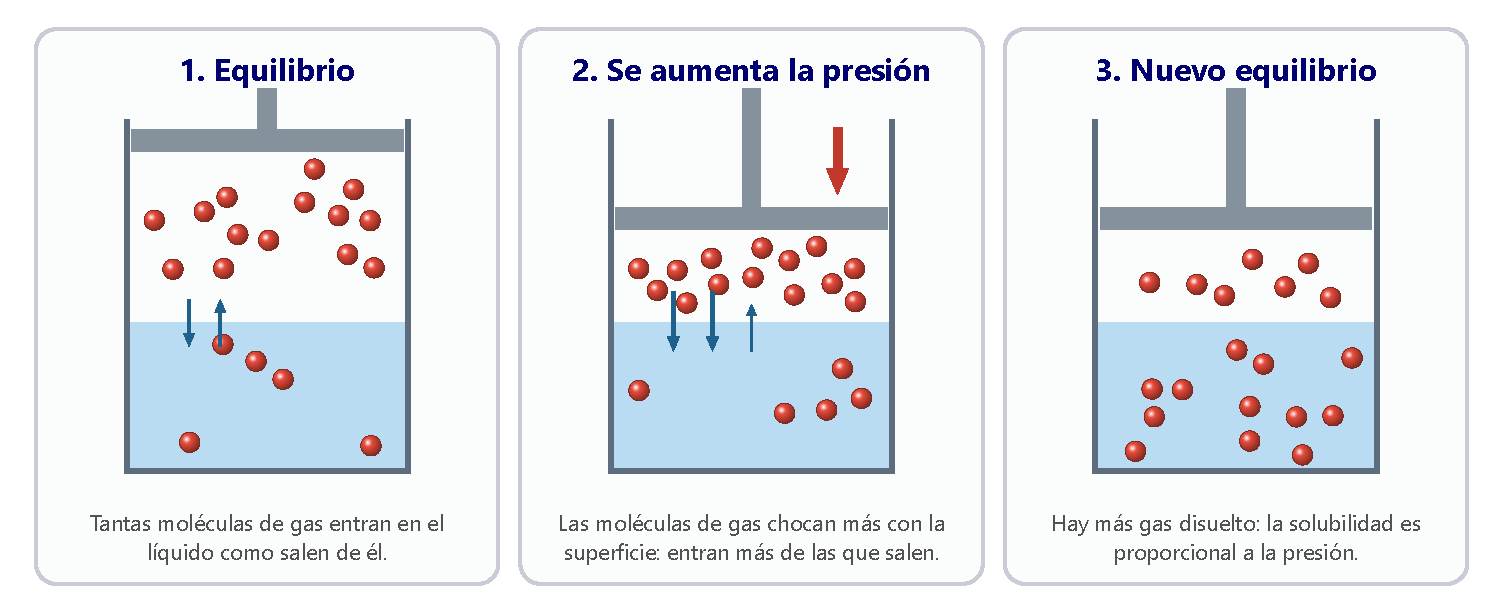
\includegraphics[width=0.95\textwidth]{images/UD2/henry}
    \caption{Al aumentar la presión de un gas sobre un líquido, aumenta la cantidad de gas disuelto.}
    \label{fig:ud2-henry}
\end{figure}

Por eso los refrescos se envasan con \ch{CO2} a varias atmósferas: al abrirlos, la presión de \ch{CO2} baja bruscamente y el
gas sobrante escapa en forma de burbujas. La ley de Henry también explica los problemas de los buceadores: a gran profundidad
respiran aire a alta presión y se disuelve mucho nitrógeno en la sangre; si suben deprisa, el gas forma burbujas
(enfermedad descompresiva).

\begin{example}
    \textbf{Nitrógeno disuelto.} Un recipiente contiene \qty{5}{\litre} de agua en contacto con aire a una presión total de
    \qty{3}{\atm}. La fracción molar del nitrógeno en el aire es \num{0.78} y su constante de Henry en agua, a esa temperatura,
    es \qty{6.4e-4}{\mol\per\litre\per\atm}. ¿Qué masa de nitrógeno hay disuelta?

    \textbf{Solución.} Presión parcial del nitrógeno: \(p(\ch{N2}) = \chi \, p_T = \num{0.78} \cdot 3 = \qty{2.34}{\atm}\).
    \[ c = k \, p = \num{6.4e-4} \cdot \num{2.34} = \qty{1.50e-3}{\mol\per\litre}; \qquad
    m = \qty{1.50e-3}{\mol\per\litre} \cdot \qty{5}{\litre} \cdot \qty{28}{\gram\per\mol} = \qty{0.21}{\gram} \]
\end{example}

\begin{exercise}
    La constante de Henry del oxígeno en agua a \qty{20}{\degreeCelsius} es \qty{1.3e-3}{\mol\per\litre\per\atm}. ¿Cuántos
    miligramos de oxígeno hay disueltos en \qty{2}{\litre} de agua en contacto con aire a \qty{1}{\atm} (21\,\% de \ch{O2})?
    \begin{solu}
        \(p(\ch{O2}) = \qty{0.21}{\atm}\); \(c = \num{1.3e-3} \cdot \num{0.21} = \qty{2.73e-4}{\mol\per\litre}\);
        \(m = \num{2.73e-4} \cdot 2 \cdot 32 = \qty{0.0175}{\gram} = \textcolor{red}{\qty{17.5}{\milli\gram}}\).
    \end{solu}
\end{exercise}

\begin{exercise}
    Explica por qué: a) un refresco pierde antes el gas si está caliente; b) en verano, en los estanques con poca agua, los peces
    suben a la superficie a «boquear».
    \begin{solu}
        a) \textcolor{red}{La solubilidad del \ch{CO2} disminuye al aumentar la temperatura}. b) \textcolor{red}{El agua caliente
        disuelve menos oxígeno}, y los peces buscan la superficie, donde el agua está en contacto con el aire.
    \end{solu}
\end{exercise}

%========================================================================================
\section{Propiedades coligativas}\label{sec:ud2-coligativas}
%========================================================================================

En invierno se echa sal en las carreteras para que no se forme hielo; al cocer pasta, el agua con sal hierve a algo más de
\qty{100}{\degreeCelsius}; y muchos alimentos se conservan en salmuera o en almíbar. Todos estos fenómenos se deben a que las
propiedades físicas de una disolución son diferentes de las del disolvente puro. Hay dos tipos de propiedades:

\begin{itemize}
    \item \textbf{Propiedades constitutivas}: dependen de la naturaleza de los componentes (densidad, viscosidad, color).
    \item \textbf{Propiedades coligativas}: dependen solo del \textbf{número de partículas} de soluto (de su concentración), y no
    de cuál sea el soluto. Son cuatro: el \textbf{descenso de la presión de vapor}, el \textbf{aumento del punto de ebullición}, el
    \textbf{descenso del punto de congelación} y la \textbf{presión osmótica}.
\end{itemize}

\subsection{Descenso de la presión de vapor}

En un líquido, algunas partículas tienen energía suficiente para escapar de la superficie y pasar a gas (\textbf{evaporación}).
En un recipiente cerrado, las partículas del vapor también chocan con la superficie y vuelven al líquido
(\textbf{condensación}). Al cabo de un tiempo se alcanza un \textbf{equilibrio dinámico}: se evaporan tantas partículas como
se condensan. La \textbf{presión de vapor} es la presión del vapor en equilibrio con su líquido; depende de la sustancia y aumenta
con la temperatura. Cuando la presión de vapor iguala la presión exterior, el líquido hierve.

Si se añade un \textbf{soluto no volátil} (que no pasa a vapor), parte de la superficie la ocupan partículas de soluto y menos
moléculas de disolvente pueden escapar: \textbf{la presión de vapor disminuye} (figura~\ref{fig:ud2-presion-vapor}).

\begin{figure}[H]
    \centering
    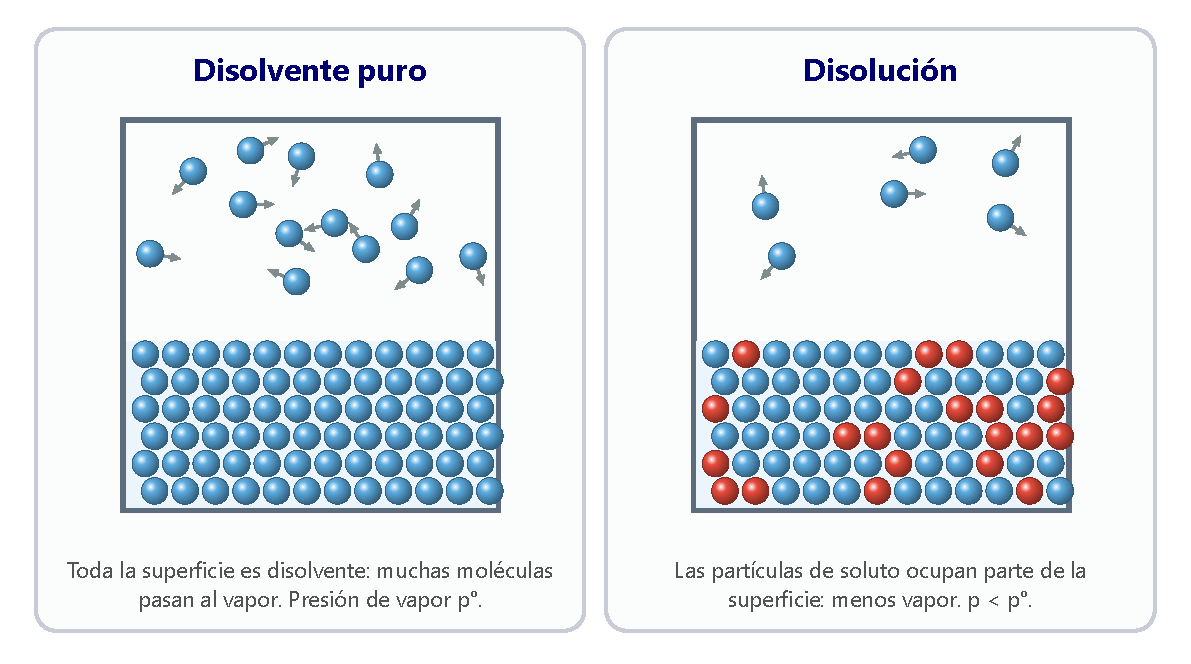
\includegraphics[width=0.75\textwidth]{images/UD2/presion_vapor}
    \caption{Un soluto no volátil hace que menos moléculas de disolvente pasen al vapor.}
    \label{fig:ud2-presion-vapor}
\end{figure}

\textbf{François-Marie Raoult} (1830-1901) midió este efecto y lo resumió en una ley:

\begin{definition}[Ley de Raoult]
    A una temperatura dada, la disminución de la presión de vapor de un disolvente al añadirle un soluto no volátil es
    proporcional a la fracción molar del soluto:
    \[ \Delta p = p^{\circ} - p = p^{\circ} \chi_s \qquad \text{o, lo que es lo mismo,} \qquad p = p^{\circ} \chi_d \]
    \(p^{\circ}\) es la presión de vapor del disolvente puro, \(p\) la de la disolución, \(\chi_s\) la fracción molar del soluto y
    \(\chi_d\) la del disolvente. Las disoluciones que cumplen exactamente esta ley se llaman \textbf{disoluciones ideales}.
\end{definition}

\begin{example}
    \textbf{Presión de vapor de una disolución de glicerina.} La presión de vapor del agua a \qty{25}{\degreeCelsius} es
    \qty{23.8}{\mmHg}. Se disuelven \qty{46}{\gram} de glicerina, \ch{C3H8O3} (no volátil), en \qty{180}{\gram} de agua.
    Calcula la presión de vapor de la disolución.

    \textbf{Solución.} \(n_{\text{glicerina}} = \dfrac{46}{92} = \qty{0.5}{\mol}\); \(n_{\text{agua}} = \dfrac{180}{18} = \qty{10}{\mol}\);
    \(\chi_s = \dfrac{\num{0.5}}{\num{10.5}} = \num{0.0476}\).
    \[ \Delta p = p^{\circ} \chi_s = \num{23.8} \cdot \num{0.0476} = \qty{1.13}{\mmHg}; \qquad p = \num{23.8} - \num{1.13} = \qty{22.7}{\mmHg} \]
\end{example}

\begin{exercise}
    La presión de vapor del etanol a \qty{50}{\degreeCelsius} es \qty{221.6}{\mmHg}. Se disuelven \qty{20}{\gram} de urea,
    \ch{CO(NH2)2}, en \qty{150}{\mL} de etanol (\(d = \qty{0.79}{\gram\per\mL}\)). ¿Cuál es la presión de vapor de la
    disolución a esa temperatura?
    \begin{solu}
        \(n_{\text{urea}} = 20/60 = \qty{0.333}{\mol}\); \(n_{\text{etanol}} = \num{118.5}/46 = \qty{2.58}{\mol}\);
        \(\chi_s = \num{0.115}\): \(\Delta p = \qty{25.4}{\mmHg}\); \(p = \textcolor{red}{\qty{196}{\mmHg}}\).
    \end{solu}
\end{exercise}

\subsection{Aumento del punto de ebullición y descenso del punto de congelación}

Como la disolución tiene menor presión de vapor, hay que calentarla más para que su presión de vapor llegue a igualar la presión
atmosférica: \textbf{la disolución hierve a una temperatura más alta} que el disolvente puro. Del mismo modo, las partículas de
soluto dificultan que las de disolvente se ordenen para formar el sólido: \textbf{la disolución congela a una temperatura más
baja} (figura~\ref{fig:ud2-diagrama}).

\begin{figure}[H]
    \centering
    \begin{tikzpicture}
        \begin{axis}[grafica, width=0.75\linewidth, height=6cm,
            xlabel={Temperatura}, ylabel={Presión de vapor},
            xmin=60, xmax=118, ymin=0, ymax=1.5, xtick=\empty, ytick={1}, yticklabels={\qty{1}{\atm}}, grid=none]
            \addplot[thick, blue!70!black, domain=60:116] {10^(8.07131 - 1730.63/(233.426 + x))/760};
            \addplot[thick, red!75!black, domain=60:116] {0.88*10^(8.07131 - 1730.63/(233.426 + x))/760};
            \addplot[dashed, gray] coordinates {(60,1) (118,1)};
            \addplot[dashed, gray] coordinates {(100,1) (100,0)};
            \addplot[dashed, gray] coordinates {(103.6,1) (103.6,0)};
            \draw[<->, thick] (axis cs:100,0.12) -- node[below, font=\small] {\(\Delta T_e\)} (axis cs:103.6,0.12);
            \draw[<->, thick] (axis cs:85,0.574) -- node[right, font=\small] {\(\Delta p\)} (axis cs:85,0.505);
            \node[font=\small, blue!70!black, anchor=east] at (axis cs:110,1.38) {disolvente puro};
            \node[font=\small, red!75!black, anchor=west] at (axis cs:110,1.0) {disolución};
            \node[font=\scriptsize, anchor=north] at (axis cs:100,0) {\(T_e\)};
            \node[font=\scriptsize, anchor=north] at (axis cs:104.4,0) {\(T_e'\)};
        \end{axis}
    \end{tikzpicture}
    \caption{La curva de presión de vapor de la disolución queda por debajo de la del disolvente: hierve a mayor temperatura.}
    \label{fig:ud2-diagrama}
\end{figure}

\begin{definition}[Ascenso ebulloscópico y descenso crioscópico]
    Para disoluciones diluidas de solutos no volátiles, las variaciones de las temperaturas de ebullición y de congelación son
    proporcionales a la \textbf{molalidad}:
    \[ \Delta T_e = T_e' - T_e = K_e \, m \qquad\qquad \Delta T_c = T_c - T_c' = K_c \, m \]
    \(T_e\) y \(T_c\) son las temperaturas del disolvente puro, y \(T_e'\) y \(T_c'\), las de la disolución. \(K_e\) es la
    \textbf{constante ebulloscópica} y \(K_c\) la \textbf{constante crioscópica}; dependen solo del disolvente.
\end{definition}

\begin{table}[H]
    \centering
    \caption{Constantes ebulloscópicas y crioscópicas de algunos disolventes (a \qty{1}{\atm})}
    \vspace{-5pt}
    \begin{tabular}{@{}lcccc@{}}
        \toprule
        \textbf{Disolvente} & \makecell{\(T_e\) \\ (\unit{\degreeCelsius})} & \makecell{\(K_e\) \\ (\unit{\degreeCelsius\kilo\gram\per\mol})} &
        \makecell{\(T_c\) \\ (\unit{\degreeCelsius})} & \makecell{\(K_c\) \\ (\unit{\degreeCelsius\kilo\gram\per\mol})} \\
        \midrule
        Agua & 100 & \num{0.52} & 0 & \num{1.86} \\[3pt]
        Benceno & \num{80.1} & \num{2.53} & \num{5.5} & \num{5.12} \\[3pt]
        Ciclohexano & \num{80.7} & \num{2.79} & \num{6.5} & \num{20.1} \\[3pt]
        Tetracloruro de carbono & \num{76.5} & \num{4.95} & \num{-22.3} & \num{29.8} \\[3pt]
        Cloroformo & \num{61.2} & \num{3.63} & \num{-63.5} & \num{4.68} \\[3pt]
        Etanol & \num{78.4} & \num{1.19} & \num{-114.6} & \num{1.99} \\[3pt]
        Alcanfor & 204 & \num{5.95} & 178 & 40 \\
        \bottomrule
    \end{tabular}
    \label{tab:ud2-constantes}
\end{table}

Estas propiedades tienen muchas aplicaciones: los \textbf{anticongelantes} (etilenglicol) del circuito de refrigeración de los
coches, la sal en las carreteras heladas o la mezcla de hielo y sal para enfriar rápidamente. Además, midiendo \(\Delta T\) se
puede calcular la \textbf{masa molar} de un soluto desconocido.

\begin{remark}
    \textbf{Solutos iónicos.} Las propiedades coligativas dependen del número de partículas. Un soluto iónico se disocia: cada
    unidad de \ch{NaCl} da dos iones (\ch{Na+} y \ch{Cl-}) y cada una de \ch{CaCl2}, tres. Por eso su efecto se multiplica por un
    factor \(i\), el \textbf{factor de van't Hoff} (\(i \approx 2\) para el \ch{NaCl}): \(\Delta T_c = i \, K_c \, m\). En los
    ejercicios de esta unidad, salvo que se diga lo contrario, los solutos son moleculares (\(i = 1\)).
\end{remark}

\begin{example}
    \textbf{Masa molar por ebulloscopia.} Al disolver \qty{9}{\gram} de una sustancia desconocida en \qty{150}{\gram} de agua,
    la temperatura de ebullición aumenta \qty{0.26}{\degreeCelsius}. Calcula la masa molar del soluto.

    \textbf{Solución.} \(m = \dfrac{\Delta T_e}{K_e} = \dfrac{\num{0.26}}{\num{0.52}} = \qty{0.5}{\mol\per\kilo\gram}\).
    Moles de soluto: \(n = m \cdot m_{\text{disolvente}} = \num{0.5} \cdot \num{0.150} = \qty{0.075}{\mol}\).
    \[ M = \frac{\qty{9}{\gram}}{\qty{0.075}{\mol}} = \qty{120}{\gram\per\mol} \]
\end{example}

\begin{example}
    \textbf{Congelación del ciclohexano.} Calcula la temperatura de congelación de una disolución de \qty{6.4}{\gram} de
    naftaleno, \ch{C10H8}, en \qty{100}{\gram} de ciclohexano.

    \textbf{Solución.} \(M(\ch{C10H8}) = \qty{128}{\gram\per\mol}\); \(m = \dfrac{\num{6.4}/128}{\num{0.1}} = \qty{0.5}{\mol\per\kilo\gram}\).
    \(\Delta T_c = K_c \, m = \num{20.1} \cdot \num{0.5} = \qty{10.05}{\degreeCelsius}\);
    \(T_c' = \num{6.5} - \num{10.05} = \qty{-3.55}{\degreeCelsius}\).
\end{example}

\begin{exercise}
    La temperatura de ebullición del etanol es \qty{78.4}{\degreeCelsius}. Si disolvemos \qty{30}{\gram} de urea,
    \ch{CO(NH2)2}, en \qty{200}{\gram} de etanol, ¿a qué temperatura hervirá la disolución?
    \begin{solu}
        \(m = \dfrac{\num{0.5}}{\num{0.2}} = \qty{2.5}{\mol\per\kilo\gram}\); \(\Delta T_e = \num{1.19} \cdot \num{2.5} = \qty{2.98}{\degreeCelsius}\):
        \(T_e' = \textcolor{red}{\qty{81.4}{\degreeCelsius}}\).
    \end{solu}
\end{exercise}

\begin{exercise}
    ¿Qué masa de maltosa, \ch{C12H22O11}, hay que disolver en \qty{250}{\gram} de agua para que su temperatura de ebullición
    aumente \qty{0.4}{\degreeCelsius}?
    \begin{solu}
        \(m = \num{0.4}/\num{0.52} = \qty{0.769}{\mol\per\kilo\gram}\); \(n = \num{0.769} \cdot \num{0.25} = \qty{0.192}{\mol}\):
        \(\textcolor{red}{\qty{65.8}{\gram}}\) de maltosa.
    \end{solu}
\end{exercise}

\begin{exercise}
    a) ¿Por qué en las zonas de montaña el agua hierve a menos de \qty{100}{\degreeCelsius}? b) ¿Por qué se echa sal en las
    carreteras heladas, y por qué no sirve cuando hace mucho frío (por debajo de unos \qty{-20}{\degreeCelsius})?
    \begin{solu}
        a) \textcolor{red}{La presión atmosférica es menor}, y la presión de vapor del agua la iguala a menor temperatura (en la
        cima del Everest, a unos \qty{70}{\degreeCelsius}). b) \textcolor{red}{La sal disuelta baja el punto de congelación del
        agua}, de modo que el hielo funde aunque la temperatura sea menor que \qty{0}{\degreeCelsius}; pero ese descenso tiene un
        límite (el de la disolución saturada, unos \qty{-21}{\degreeCelsius}).
    \end{solu}
\end{exercise}

\subsection{Presión osmótica}

Una \textbf{membrana semipermeable} deja pasar las moléculas de disolvente, pero no las de soluto. Si separa dos disoluciones de
distinta concentración, el disolvente pasa de la \textbf{más diluida a la más concentrada}, hasta que las concentraciones se
igualan o el nivel que sube compensa el proceso (figura~\ref{fig:ud2-osmosis}). Este fenómeno se llama \textbf{ósmosis} y es
fundamental en biología: así se intercambia agua a través de las membranas de las células.

\begin{definition}[Presión osmótica]
    Es la presión, \(\pi\), que hay que ejercer sobre la disolución más concentrada para impedir el paso neto de disolvente a través
    de la membrana. \textbf{Van't Hoff} (1852-1911) descubrió que, en disoluciones diluidas, cumple una ecuación igual a la de los
    gases ideales:
    \[ \pi V = n R T \quad \Rightarrow \quad \pi = \frac{n}{V} R T = c \, R \, T \]
    donde \(c\) es la concentración molar y \(T\), la temperatura absoluta.
\end{definition}

\begin{figure}[H]
    \centering
    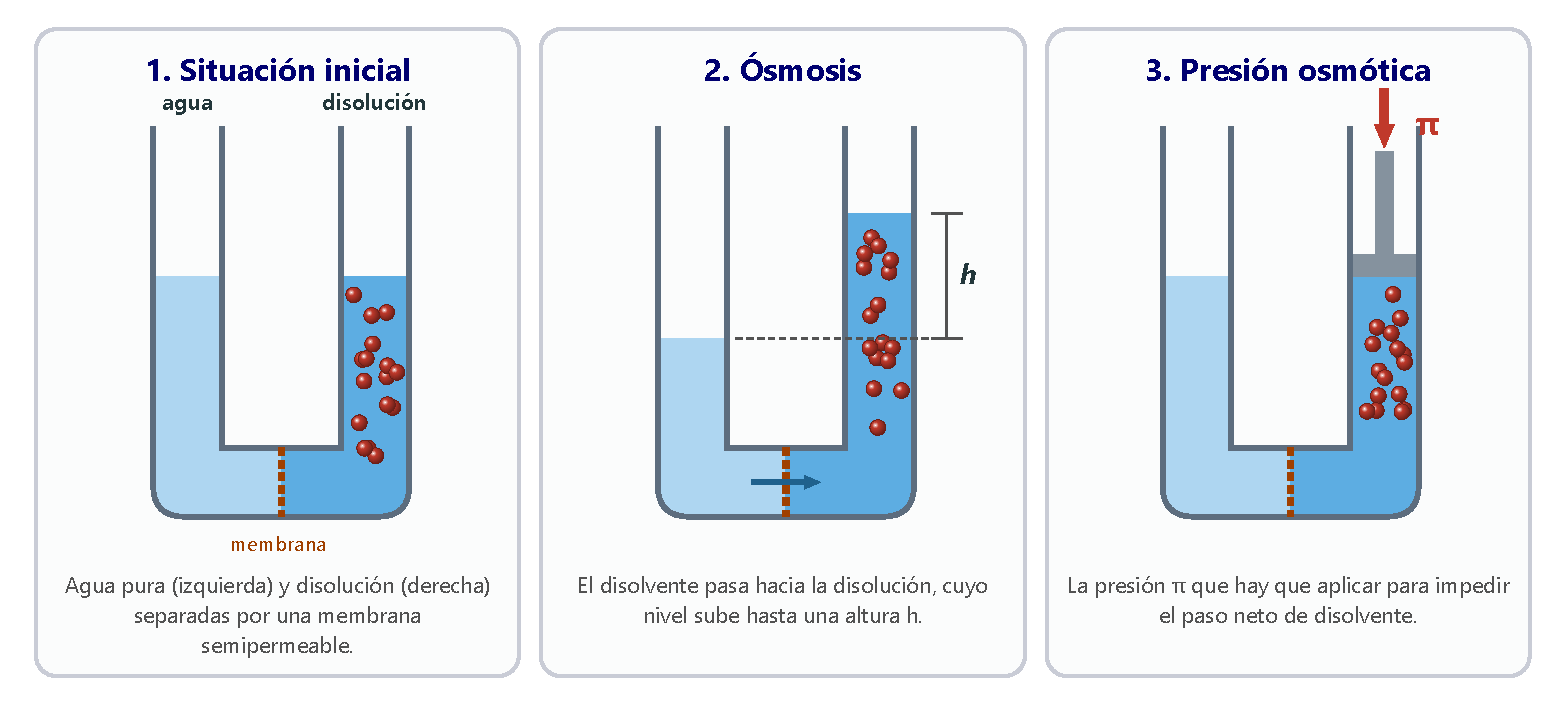
\includegraphics[width=0.95\textwidth]{images/UD2/osmosis}
    \caption{Ósmosis y presión osmótica.}
    \label{fig:ud2-osmosis}
\end{figure}

La presión osmótica es fácil de medir y alcanza valores grandes incluso con concentraciones pequeñas; por eso se usa para
determinar masas molares de sustancias de masa molar muy alta, como las proteínas.

\paragraph{Disoluciones isotónicas, hipertónicas e hipotónicas.} Dos disoluciones con la misma presión osmótica son
\textbf{isotónicas}. Si una tiene mayor presión osmótica que otra de referencia, es \textbf{hipertónica}; si la tiene menor,
\textbf{hipotónica}. Las células se comportan de forma distinta según el medio que las rodea (figura~\ref{fig:ud2-tonicidad}):
en un medio hipertónico pierden agua y se arrugan; en uno hipotónico, la ganan y pueden llegar a romperse. Por eso los sueros y
los medicamentos inyectables son disoluciones isotónicas con la sangre.

\begin{figure}[H]
    \centering
    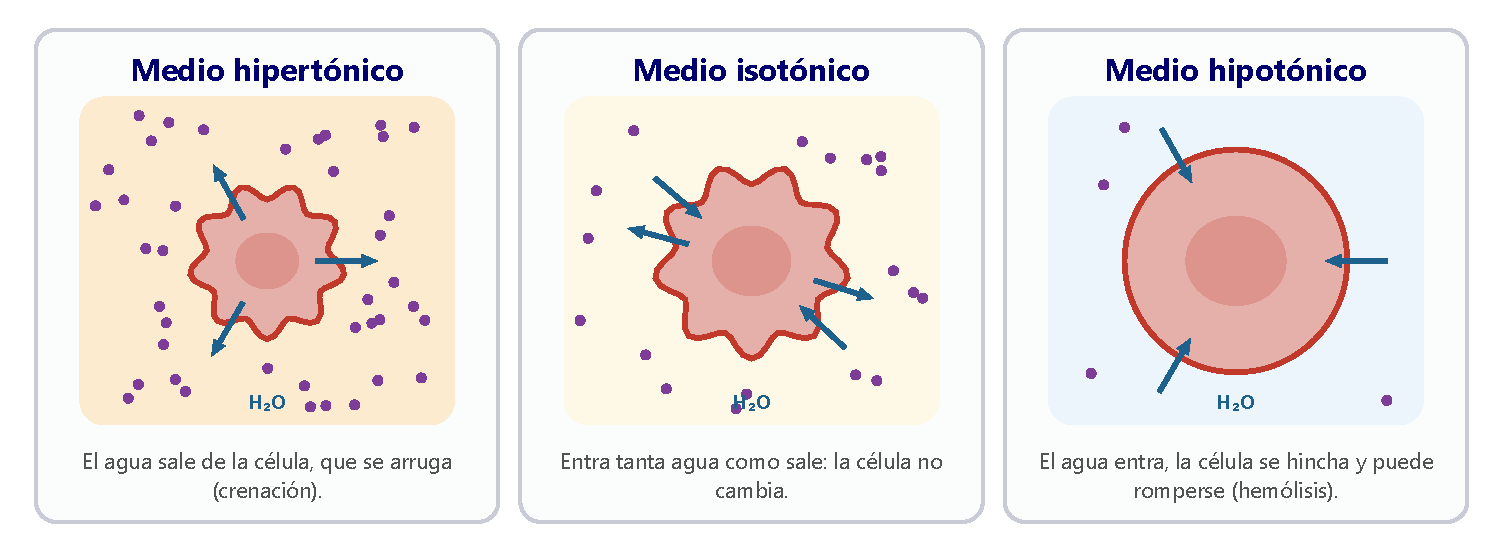
\includegraphics[width=0.95\textwidth]{images/UD2/tonicidad}
    \caption{Glóbulos rojos en disoluciones hipertónica, isotónica e hipotónica.}
    \label{fig:ud2-tonicidad}
\end{figure}

\paragraph{Ósmosis inversa.} Si sobre la disolución más concentrada se aplica una presión \textbf{mayor} que la osmótica, el
disolvente pasa en sentido contrario, de la disolución concentrada a la diluida. Es la \textbf{ósmosis inversa}, que usan las
plantas \textbf{desaladoras} para obtener agua potable a partir de agua de mar (figura~\ref{fig:ud2-inversa}) y muchos
purificadores domésticos.

\begin{figure}[H]
    \centering
    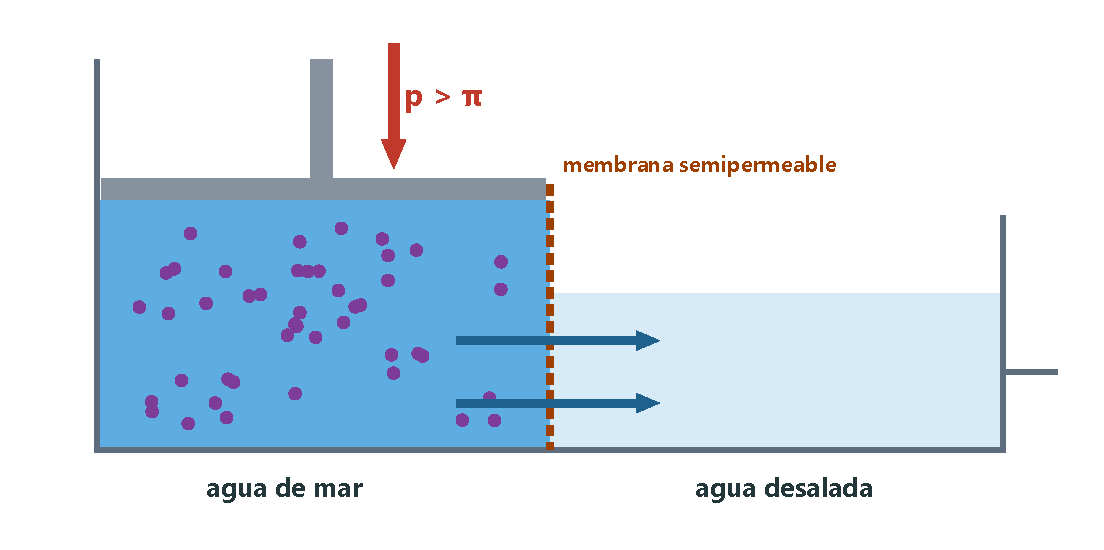
\includegraphics[width=0.65\textwidth]{images/UD2/osmosis_inversa}
    \caption{Ósmosis inversa en una planta desaladora.}
    \label{fig:ud2-inversa}
\end{figure}

\begin{example}
    \textbf{Presión osmótica y masa molar.} a) Calcula la presión osmótica de una disolución de glucosa \qty{0.3}{\mol\per\litre}
    a \qty{37}{\degreeCelsius}. b) Una disolución de \qty{250}{\mL} que contiene \qty{4}{\gram} de un soluto desconocido tiene,
    a \qty{25}{\degreeCelsius}, una presión osmótica de \qty{3000}{\mmHg}. ¿Cuál es la masa molar del soluto?

    \textbf{Solución.} a) \(\pi = c R T = \num{0.3} \cdot \num{0.082} \cdot 310 = \qty{7.63}{\atm}\).

    b) \(\pi = \dfrac{3000}{760} = \qty{3.95}{\atm}\). De \(\pi V = \dfrac{m}{M} R T\):
    \[ M = \frac{m R T}{\pi V} = \frac{4 \cdot \num{0.082} \cdot 298}{\num{3.95} \cdot \num{0.25}} = \qty{99}{\gram\per\mol} \]
\end{example}

\begin{example}
    \textbf{¿Por qué no podemos beber agua de mar?}

    \textbf{Solución.} El agua de mar tiene una concentración de sales mucho mayor que la de nuestros líquidos corporales: es un
    medio \textbf{hipertónico}. Al beberla, las células tienden a igualar concentraciones cediendo agua por ósmosis; además, los
    riñones necesitan más agua para eliminar el exceso de sal de la que se ha bebido. El resultado es que nos
    \textbf{deshidratamos}.
\end{example}

\begin{exercise}
    Investiga qué técnicas de conservación de alimentos se basan en la presión osmótica (salazón, almíbar, salmuera…). ¿Por qué
    la lechuga aliñada con sal se ablanda al cabo de un rato?
    \begin{solu}
        \textcolor{red}{En un medio muy concentrado (hipertónico), los microorganismos pierden agua por ósmosis y no pueden
        crecer}: así se conservan las salazones, las mermeladas o las frutas en almíbar. \textcolor{red}{La sal forma una disolución
        hipertónica sobre la lechuga}: sus células pierden agua y la hoja se arruga y se ablanda.
    \end{solu}
\end{exercise}

\begin{exercise}
    Los riñones filtran la sangre para eliminar sustancias de desecho. Cuando fallan, los pacientes se someten a
    \textbf{diálisis}. Investiga en qué consiste y en qué se parece a la ósmosis.
    \begin{solu}
        \textcolor{red}{En la diálisis la sangre circula junto a un líquido de diálisis, separados por una membrana semipermeable}
        con poros que dejan pasar el agua y las moléculas pequeñas (urea, sales en exceso), pero no las células ni las proteínas.
        Los desechos pasan de la sangre, donde están más concentrados, al líquido de diálisis. Se parece a la ósmosis en el uso de
        la membrana, pero en la diálisis atraviesan la membrana \textbf{solutos}, no solo el disolvente.
    \end{solu}
\end{exercise}

%========================================================================================
\section{Química en la vida: cómo limpiar la casa con productos de la cocina}\label{sec:ud2-limpieza}
%========================================================================================

Muchos productos de limpieza son disoluciones de sustancias contaminantes que, en ocasiones, podemos sustituir por otras más
sencillas. Algunos ejemplos:

\begin{itemize}
    \item \textbf{Superficies metálicas oxidadas}: unas gotas de \textbf{zumo de limón} o de pomelo. Su ácido cítrico reacciona con
    los óxidos y los convierte en sales solubles en agua.
    \item \textbf{Parrilla del horno con óxido}: frotarla con media \textbf{cebolla}. Al frotar se libera agua con aminoácidos y
    enzimas que ayudan a disolver los óxidos adheridos.
    \item \textbf{Suelos de madera}: un poco de \textbf{té negro} en el agua de fregar. El té contiene \textbf{taninos}, los mismos
    que hay en la corteza de los árboles, que desinfectan y devuelven el color a la madera.
    \item \textbf{Baño}: \textbf{vinagre}, una disolución acuosa de ácido acético (en torno al 5\,\%). Disuelve la cal y, al ser
    ácido, impide que crezcan muchos microorganismos.
\end{itemize}

\begin{exercise}
    a) El vinagre de limpieza tiene un 6\,\% en masa de ácido acético, \ch{CH3COOH}, y una densidad de \qty{1.01}{\gram\per\mL}.
    Calcula su concentración molar. b) ¿Por qué el vinagre elimina la cal (carbonato de calcio) de los grifos? c) ¿Qué ventaja
    ambiental tiene usar estos productos?
    \begin{solu}
        a) \(c = \dfrac{\num{0.06} \cdot 1010}{60} = \textcolor{red}{\qty{1.01}{\mol\per\litre}}\). b) \textcolor{red}{Porque el
        ácido reacciona con el carbonato de calcio} y forma acetato de calcio, soluble en agua, y dióxido de carbono.
        c) \textcolor{red}{Son biodegradables, baratos y no contaminan el agua} con tensioactivos, fosfatos o disolventes.
    \end{solu}
\end{exercise}

%========================================================================================
\section{Prácticas}\label{sec:ud2-practicas}
%========================================================================================

\subsection{Preparación de una disolución de sulfato de cobre(II)}

\begin{multicols}{2}
    \textbf{Objetivo}
    \begin{itemize}
        \item Preparar \qty{250}{\mL} de una disolución de \ch{CuSO4} \qty{0.1}{\mol\per\litre} y, a partir de ella, otra diluida.
    \end{itemize}
    \columnbreak
    \textbf{Material y reactivos}
    \begin{itemize}
        \item Balanza, vidrio de reloj, espátula, vaso de precipitados, varilla, embudo, frasco lavador, cuentagotas, pipeta
        con aspirador y matraces aforados de 250 y \qty{100}{\mL}.
        \item Sulfato de cobre(II) anhidro y agua destilada.
    \end{itemize}
\end{multicols}

\textbf{Procedimiento}
\begin{enumerate}[label=\numberballgreen]
    \item Calcula la masa de \ch{CuSO4} necesaria (ejemplo de la sección~\ref{sec:ud2-preparacion}) y prepara la disolución siguiendo
    los pasos de la figura~\ref{fig:ud2-prep-solido}. \textbf{Usa guantes y gafas: el sulfato de cobre es nocivo.}
    \item Calcula el volumen de esa disolución que necesitas para preparar \qty{100}{\mL} de disolución
    \qty{0.02}{\mol\per\litre}. Tómalo con la pipeta, viértelo en el matraz de \qty{100}{\mL} y enrasa.
    \item Compara el color de las dos disoluciones y etiquétalas.
\end{enumerate}

\begin{exercise}
    a) ¿Qué volumen de la disolución \qty{0.1}{\mol\per\litre} necesitas en el paso 2? b) ¿Por qué el color de la disolución
    diluida es más claro? c) Si al enrasar el menisco queda por encima de la marca, ¿la concentración será mayor o menor que la
    calculada?
    \begin{solu}
        a) \(V_1 = \dfrac{\num{0.02} \cdot 100}{\num{0.1}} = \textcolor{red}{\qty{20}{\mL}}\). b) \textcolor{red}{Hay menos iones
        \ch{Cu^2+} (responsables del color azul) por unidad de volumen}. c) \textcolor{red}{Menor}: el mismo soluto ocupa un volumen
        mayor.
    \end{solu}
\end{exercise}

\subsection{¿Cómo enfriar una lata de refresco en menos de diez minutos?}

\begin{multicols}{2}
    \textbf{Objetivo}
    \begin{itemize}
        \item Comprobar el descenso del punto de congelación del agua al añadir sal o alcohol.
    \end{itemize}
    \columnbreak
    \textbf{Material}
    \begin{itemize}
        \item Tres cuencos grandes, tres latas iguales de la misma bebida, hielo picado, sal, \qty{100}{\mL} de alcohol y un
        termómetro.
    \end{itemize}
\end{multicols}

\textbf{Procedimiento}
\begin{enumerate}[label=\numberballgreen]
    \item \textbf{Cuenco 1}: un puñado de hielo picado que cubra el fondo y un poco de agua.
    \item \textbf{Cuenco 2}: la misma cantidad de hielo y agua, y un buen puñado de sal.
    \item \textbf{Cuenco 3}: la misma cantidad de hielo, \qty{100}{\mL} de agua y \qty{100}{\mL} de alcohol.
    \item Introduce una lata en cada cuenco, espera diez minutos y mide la temperatura de cada mezcla y de cada bebida.
\end{enumerate}

\begin{exercise}
    a) ¿En qué cuencos baja más la temperatura? ¿Por qué? b) ¿Qué propiedad coligativa explica el experimento? c) Cita otra
    situación cotidiana en la que se use para enfriar o descongelar algo.
    \begin{solu}
        a) \textcolor{red}{En los cuencos 2 y 3}: la sal o el alcohol disueltos bajan el punto de congelación del agua; el hielo
        sigue fundiendo por debajo de \qty{0}{\degreeCelsius} y, para fundir, toma calor de la mezcla y de la lata, que se enfrían
        mucho más que con hielo solo. b) \textcolor{red}{El descenso crioscópico}. c) \textcolor{red}{Echar sal en las carreteras
        heladas, los anticongelantes de los coches} o las heladeras artesanas de hielo y sal.
    \end{solu}
\end{exercise}

%========================================================================================
\section{Situación de aprendizaje: agua limpia y saneamiento (ODS 6)}\label{sec:ud2-ods}
%========================================================================================

El \textbf{Objetivo de Desarrollo Sostenible 6} busca garantizar el acceso de todas las personas al agua potable y al
saneamiento, y una gestión sostenible del agua. España es uno de los países europeos más amenazados por la sequía: los expertos
advierten de que, con el calentamiento global, los periodos secos serán cada vez más largos. Algunas empresas de abastecimiento
calculan que cada persona gasta en casa unos \qty{140}{\litre} de agua al día, y se ha propuesto reducir ese consumo a unos
\qty{100}{\litre}.

\begin{marker}
    \textbf{Reto:} calculad vuestro consumo de agua y vuestra huella hídrica, y proponed medidas para reducirlos.
\end{marker}

\begin{enumerate}[label=\numberballred]
    \item \textbf{¿Cuánta agua consumes cada día?} Estima tu consumo con estos datos aproximados: grifo abierto, \qty{12}{\litre}
    por minuto; ducha, \qty{60}{\litre} en 5 minutos; cisterna, de 6 a \qty{12}{\litre} por descarga; lavar los platos a mano con
    el grifo abierto, unos \qty{100}{\litre}. ¿Qué acciones podrías cambiar para reducirlo?
    \item \textbf{Huella hídrica.} El agua que gastamos no es solo la del grifo: también la que se usa para producir lo que
    comemos o vestimos. Por ejemplo, producir \qty{1}{\kilo\gram} de carne de ternera requiere unos \qty{15000}{\litre};
    \qty{1}{\kilo\gram} de chocolate, unos \qty{17000}{\litre}; unos pantalones vaqueros, unos \qty{8000}{\litre}; y
    \qty{1}{\kilo\gram} de tomates, unos \qty{200}{\litre}. Buscad la huella hídrica de lo que coméis en un día y de la ropa que
    lleváis puesta.
    \item \textbf{Las desaladoras.} Investigad cómo funcionan las plantas desaladoras de ósmosis inversa de España: cuánta agua
    producen, cuánta energía consumen y qué se hace con la salmuera que generan.
    \item \textbf{Debate.} En pequeños grupos, proponed cuatro acciones cotidianas que reduzcan de verdad el gasto de agua, como
    consumidores o cambiando hábitos de consumo, y presentadlas al resto de la clase.
\end{enumerate}

    \newpage
    %! Unidad 2 — Disoluciones: ejercicios resueltos y ejercicios finales
%! Fuente: Fuentes/Quimica/Unidad 2 («Ejercicios resueltos», «Practica y calcula», «Piensa y resuelve»).
%! Enunciados adaptados con datos cambiados; soluciones recalculadas. Dificultad: \(\star\) baja, \(\star\star\) media, \(\star\star\star\) alta.
%! En las propiedades coligativas se han cambiado los solutos iónicos por moleculares (salvo en los ejercicios con factor de van't Hoff).

\section{Ejercicios resueltos}\label{sec:ud2-resueltos}

Salvo que se indique otra cosa, usa las masas atómicas H = 1; C = 12; N = 14; O = 16; Na = 23; S = 32; Cl = 35,5; K = 39;
Ca = 40; y \(R = \qty{0.082}{\atm\litre\per\mol\per\kelvin}\).

\begin{example}
    \textbf{Ácido acético comercial.} Una botella de ácido acético, \ch{CH3COOH}, indica: «98\,\% en masa;
    \(d = \qty{1.05}{\gram\per\mL}\)». Calcula: a) su concentración molar; b) su concentración en \unit{\gram\per\litre};
    c) la molalidad de una disolución preparada mezclando \qty{15}{\mL} de este ácido con \qty{85}{\mL} de agua; d) el volumen
    de ácido comercial necesario para preparar \qty{500}{\mL} de disolución \qty{0.3}{\mol\per\litre}.

    \textbf{Solución.} \textbf{1. Datos}: riqueza 98\,\%, \(d = \qty{1.05}{\gram\per\mL}\), \(M = \qty{60}{\gram\per\mol}\).

    \textbf{2. Cálculos.} a) Partimos de \qty{100}{\gram} de disolución (98 g de ácido) y encadenamos factores:
    \[ c = \frac{\qty{98}{\gram}\ \text{ácido}}{\qty{100}{\gram}\ \text{dis.}} \cdot \frac{\qty{1}{\mol}}{\qty{60}{\gram}} \cdot
    \frac{\qty{1.05}{\gram}\ \text{dis.}}{\qty{1}{\mL}} \cdot \frac{\qty{1000}{\mL}}{\qty{1}{\litre}} = \qty{17.15}{\mol\per\litre} \]

    b) \(\gamma = \num{0.98} \cdot \qty{1050}{\gram\per\litre} = \qty{1029}{\gram\per\litre}\).

    c) Moles en los \qty{15}{\mL}: \(n = \num{17.15} \cdot \num{0.015} = \qty{0.257}{\mol}\). El disolvente son los \qty{85}{\gram}
    de agua añadidos (el agua que trae el ácido, \(15 \cdot \num{1.05} \cdot \num{0.02} = \qty{0.3}{\gram}\), es despreciable):
    \[ m = \frac{\qty{0.257}{\mol}}{\qty{0.085}{\kilo\gram}} = \qty{3.0}{\mol\per\kilo\gram} \]

    d) Moles necesarios: \(\num{0.3} \cdot \num{0.5} = \qty{0.15}{\mol}\); volumen de ácido comercial:
    \(V = \dfrac{\num{0.15}}{\num{17.15}} = \qty{8.75e-3}{\litre} = \qty{8.75}{\mL}\). Se toman con una pipeta, se vierten en un
    matraz aforado de \qty{500}{\mL} con algo de agua y se enrasa.
\end{example}

\begin{example}
    \textbf{Solubilidad del nitrato de sodio.} La solubilidad del nitrato de sodio a \qty{20}{\degreeCelsius} es de
    \qty{88}{\gram} por cada \qty{100}{\gram} de agua. a) ¿Cuántos gramos se pueden disolver como máximo en \qty{350}{\gram} de
    agua a esa temperatura? b) ¿Cuánto nitrato hay que añadir a \qty{0.6}{\kilo\gram} de agua para que la disolución quede
    saturada? c) ¿Será mayor o menor su solubilidad a \qty{60}{\degreeCelsius}?

    \textbf{Solución.} La solubilidad es una proporción: \qty{0.88}{\gram} de soluto por cada gramo de agua.

    a) \(\qty{350}{\gram}\ \text{agua} \cdot \dfrac{\qty{88}{\gram}}{\qty{100}{\gram}\ \text{agua}} = \qty{308}{\gram}\); si añadiéramos más,
    el exceso precipitaría.

    b) \(\qty{600}{\gram} \cdot \num{0.88} = \qty{528}{\gram}\) de nitrato de sodio.

    c) Como la de la mayoría de los sólidos, su solubilidad \textbf{aumenta} con la temperatura (a \qty{60}{\degreeCelsius} es de
    unos \qty{124}{\gram} por \qty{100}{\gram} de agua): las partículas se mueven más y la solvatación es más eficaz.
\end{example}

\begin{example}
    \textbf{Ley de Raoult.} A \qty{25}{\degreeCelsius}, la presión de vapor del agua es \qty{23.76}{\mmHg}, y la de una
    disolución acuosa de glucosa, \qty{21.40}{\mmHg}. a) ¿Cuál es la fracción molar de la glucosa? b) ¿Cuántos gramos de glucosa
    hay disueltos por cada \qty{100}{\gram} de agua?

    \textbf{Solución.} a) \(\Delta p = \num{23.76} - \num{21.40} = \qty{2.36}{\mmHg}\). Por la ley de Raoult:
    \[ \chi_s = \frac{\Delta p}{p^{\circ}} = \frac{\num{2.36}}{\num{23.76}} = \num{0.0993} \]
    La glucosa es el 9,9\,\% de los moles de la disolución, y el agua, el 90,1\,\%.

    b) En \qty{100}{\gram} de agua hay \(100/18 = \qty{5.56}{\mol}\). De \(\chi_s = \dfrac{n_s}{n_s + n_d}\):
    \(n_s = \dfrac{\chi_s \, n_d}{1 - \chi_s} = \dfrac{\num{0.0993} \cdot \num{5.56}}{\num{0.9007}} = \qty{0.613}{\mol}\), es decir,
    \(\num{0.613} \cdot 180 = \qty{110}{\gram}\) de glucosa.
\end{example}

\begin{example}
    \textbf{Mezcla de disoluciones.} Se mezclan \qty{150}{\mL} de una disolución de \ch{CaCl2} \qty{1.2}{\mol\per\litre} con
    \qty{250}{\mL} de otra \qty{2}{\mol\per\litre} del mismo soluto. a) ¿Cuál es la concentración de la mezcla? b) ¿Y si después
    se añaden \qty{100}{\mL} de agua? Supón volúmenes aditivos.

    \textbf{Solución.} a) Los moles de soluto se suman: \(n = \num{1.2} \cdot \num{0.15} + 2 \cdot \num{0.25} = \num{0.18} + \num{0.5} = \qty{0.68}{\mol}\),
    en \qty{0.4}{\litre}: \(c = \dfrac{\num{0.68}}{\num{0.4}} = \qty{1.7}{\mol\per\litre}\). La concentración queda entre las dos
    iniciales, más cerca de la de la disolución de la que se toma más volumen.

    b) El agua no aporta soluto: \(c = \dfrac{\num{0.68}}{\num{0.5}} = \qty{1.36}{\mol\per\litre}\).
\end{example}

\begin{example}
    \textbf{El anticongelante del coche.} El circuito de refrigeración de un coche contiene \qty{4}{\litre} de agua a los que se
    añaden \qty{0.5}{\litre} de etilenglicol, \ch{C2H6O2} (\(d = \qty{1.11}{\gram\per\mL}\)). Calcula las temperaturas de
    congelación y de ebullición del líquido.

    \textbf{Solución.} \(M(\ch{C2H6O2}) = \qty{62}{\gram\per\mol}\); \(m_{\text{etilenglicol}} = 500 \cdot \num{1.11} = \qty{555}{\gram}\);
    \(n = 555/62 = \qty{8.95}{\mol}\). Molalidad: \(m = \dfrac{\num{8.95}}{4} = \qty{2.24}{\mol\per\kilo\gram}\).
    \[ \Delta T_c = \num{1.86} \cdot \num{2.24} = \qty{4.16}{\degreeCelsius} \Rightarrow T_c' = \qty{-4.2}{\degreeCelsius}; \qquad
    \Delta T_e = \num{0.52} \cdot \num{2.24} = \qty{1.16}{\degreeCelsius} \Rightarrow T_e' = \qty{101.2}{\degreeCelsius} \]
    El anticongelante protege el motor de las heladas y también evita que el líquido hierva con facilidad.
\end{example}

%========================================================================================
\section{Ejercicios de aplicación}\label{sec:ud2-aplicacion}
%========================================================================================

\subsection{Porcentaje en masa, en volumen y concentración en masa}

\begin{exercise}
    \(\star\) Queremos preparar una disolución al 25\,\% en masa. a) Si tenemos \qty{40}{\gram} de soluto, ¿cuál será la masa de
    la disolución? b) ¿Cuánto soluto hay en \qty{60}{\gram} de disolución?
    \begin{solu}
        a) \(40 \cdot \dfrac{100}{25} = \textcolor{red}{\qty{160}{\gram}}\). b) \(60 \cdot \num{0.25} = \textcolor{red}{\qty{15}{\gram}}\).
    \end{solu}
\end{exercise}

\begin{exercise}
    \(\star\) Disolvemos \qty{40}{\gram} de \ch{KCl} en \qty{150}{\mL} de agua. ¿Cuál es el porcentaje en masa de la disolución?
    \begin{solu}
        \(\% = \dfrac{40}{190} \cdot 100 = \textcolor{red}{\qty{21.1}{\percent}}\).
    \end{solu}
\end{exercise}

\begin{exercise}
    \(\star\) Un medicamento es una disolución de \qty{200}{\gram\per\litre} y densidad \qty{1.15}{\gram\per\mL}. Calcula: a) su
    porcentaje en masa; b) la masa de soluto que hay en \qty{120}{\gram} de disolución; c) el volumen de disolución que contiene
    \qty{30}{\gram} de soluto.
    \begin{solu}
        a) En \qty{1}{\litre}: \qty{200}{\gram} de soluto en \qty{1150}{\gram}: \(\textcolor{red}{\qty{17.4}{\percent}}\).
        b) \(120 \cdot \num{0.174} = \textcolor{red}{\qty{20.9}{\gram}}\). c) \(30/200 = \qty{0.15}{\litre} = \textcolor{red}{\qty{150}{\mL}}\).
    \end{solu}
\end{exercise}

\begin{exercise}
    \(\star\star\) Una disolución de ibuprofeno tiene un 30\,\% en masa de principio activo y una densidad de
    \qty{1.25}{\gram\per\mL}. a) ¿Cuál es su concentración en \unit{\milli\gram\per\mL}? b) ¿Qué volumen contiene
    \qty{600}{\milli\gram} de ibuprofeno? c) ¿Cuánto ibuprofeno hay en \qty{4}{\mL}?
    \begin{solu}
        a) \(\num{0.30} \cdot 1250 = \textcolor{red}{\qty{375}{\milli\gram\per\mL}}\). b) \(600/375 = \textcolor{red}{\qty{1.6}{\mL}}\).
        c) \(4 \cdot 375 = \qty{1500}{\milli\gram} = \textcolor{red}{\qty{1.5}{\gram}}\).
    \end{solu}
\end{exercise}

\begin{exercise}
    \(\star\star\) La digoxina se usa para tratar arritmias cardíacas. A un paciente se le administran \qty{8}{\mL} de una
    disolución de digoxina de \qty{0.3}{\milli\gram} por cada \qty{5}{\mL}. ¿Cuál es la concentración en \unit{\gram\per\litre}?
    ¿Qué masa de digoxina ha recibido?
    \begin{solu}
        \(\gamma = \dfrac{\qty{0.3e-3}{\gram}}{\qty{5e-3}{\litre}} = \textcolor{red}{\qty{0.06}{\gram\per\litre}}\);
        \(m = 8 \cdot \dfrac{\num{0.3}}{5} = \textcolor{red}{\qty{0.48}{\milli\gram}}\).
    \end{solu}
\end{exercise}

\begin{exercise}
    \(\star\star\) Un vial de un anestésico local tiene una concentración del 2\,\% en masa. ¿Qué volumen hay que inyectar si la
    dosis prescrita es de \qty{120}{\milli\gram}? Supón que la densidad de la disolución es \qty{1}{\gram\per\mL}.
    \begin{solu}
        \(m_{\text{disolución}} = \dfrac{\num{0.120}}{\num{0.02}} = \qty{6}{\gram}\): \(\textcolor{red}{\qty{6}{\mL}}\).
    \end{solu}
\end{exercise}

\begin{exercise}
    \(\star\star\) ¿Cuántos gramos de glucosa hay en una bolsa de \qty{250}{\mL} de suero glucosado al 5\,\%? ¿Y de cloruro de
    sodio en una de \qty{500}{\mL} de suero fisiológico al 0,9\,\%? (Densidad de los sueros \(\approx \qty{1}{\gram\per\mL}\).)
    \begin{solu}
        \(250 \cdot \num{0.05} = \textcolor{red}{\qty{12.5}{\gram}}\) de glucosa; \(500 \cdot \num{0.009} = \textcolor{red}{\qty{4.5}{\gram}}\) de \ch{NaCl}.
    \end{solu}
\end{exercise}

\begin{exercise}
    \(\star\star\) La atropina se usa como antídoto en intoxicaciones por insecticidas. Se dispone de una disolución de
    \qty{4}{\gram} de atropina en \qty{100}{\mL}. ¿Cuál es su concentración en \unit{\gram\per\litre}? ¿Qué volumen hay que
    administrar para una dosis de \qty{200}{\milli\gram}?
    \begin{solu}
        \(\gamma = \textcolor{red}{\qty{40}{\gram\per\litre}}\) (\qty{40}{\milli\gram\per\mL}); \(V = 200/40 = \textcolor{red}{\qty{5}{\mL}}\).
    \end{solu}
\end{exercise}

\begin{exercise}
    \(\star\star\) A una niña de \qty{30}{\kilo\gram} hay que administrarle un medicamento a razón de \qty{20}{\milli\gram} por
    kilogramo de masa corporal. ¿Qué masa de medicamento le corresponde? Expresa la dosis como porcentaje en masa respecto a su
    masa corporal.
    \begin{solu}
        \(m = 30 \cdot 20 = \textcolor{red}{\qty{600}{\milli\gram}}\); \(\dfrac{\qty{20}{\milli\gram}}{\qty{1e6}{\milli\gram}} \cdot 100 =
        \textcolor{red}{\qty{2e-3}{\percent}}\).
    \end{solu}
\end{exercise}

\subsection{Concentración molar, molalidad y fracción molar}

\begin{exercise}
    \(\star\star\) Tenemos \qty{400}{\mL} de una disolución de \ch{HCl} \qty{0.4}{\mol\per\litre}. Determina: a) la masa de
    \ch{HCl} que contiene; b) el volumen de disolución que contiene \qty{365}{\milli\gram} de \ch{HCl}; c) su molalidad, si su
    densidad es \qty{1.02}{\gram\per\mL}.
    \begin{solu}
        a) \(n = \qty{0.16}{\mol}\): \(\textcolor{red}{\qty{5.84}{\gram}}\). b) \(\qty{0.01}{\mol}/\num{0.4} = \textcolor{red}{\qty{25}{\mL}}\).
        c) En \qty{1}{\litre}: \qty{1020}{\gram} de disolución, \(\num{0.4} \cdot \num{36.5} = \qty{14.6}{\gram}\) de \ch{HCl} y
        \qty{1005.4}{\gram} de agua: \(m = \textcolor{red}{\qty{0.398}{\mol\per\kilo\gram}}\).
    \end{solu}
\end{exercise}

\begin{exercise}
    \(\star\) Una mezcla contiene \qty{20}{\gram} de \ch{NaCl}, \qty{50}{\gram} de \ch{PbCl2} y \qty{10}{\gram} de \ch{NaOH}.
    Calcula la fracción molar de cada componente.
    \begin{solu}
        \(n(\ch{NaCl}) = \qty{0.342}{\mol}\); \(n(\ch{PbCl2}) = 50/\num{278.2} = \qty{0.180}{\mol}\); \(n(\ch{NaOH}) = \qty{0.25}{\mol}\); total \qty{0.772}{\mol}.
        \(\chi(\ch{NaCl}) = \textcolor{red}{\num{0.443}}\); \(\chi(\ch{PbCl2}) = \textcolor{red}{\num{0.233}}\); \(\chi(\ch{NaOH}) = \textcolor{red}{\num{0.324}}\).
    \end{solu}
\end{exercise}

\begin{exercise}
    \(\star\star\) En una disolución acuosa de \ch{KCl}, la fracción molar del soluto es \num{0.05}. Si se han usado
    \qty{400}{\gram} de agua, calcula: a) la masa de \ch{KCl}; b) la molalidad; c) la concentración molar, si la densidad es
    \qty{1.10}{\gram\per\mL}.
    \begin{solu}
        a) \(n_{\text{agua}} = \qty{22.2}{\mol}\); \(n_s = \dfrac{\num{0.05} \cdot \num{22.2}}{\num{0.95}} = \qty{1.17}{\mol}\):
        \(\textcolor{red}{\qty{87.3}{\gram}}\). b) \(\num{1.17}/\num{0.4} = \textcolor{red}{\qty{2.92}{\mol\per\kilo\gram}}\).
        c) \(V = \num{487.3}/\num{1.10} = \qty{443}{\mL}\): \(c = \textcolor{red}{\qty{2.64}{\mol\per\litre}}\).
    \end{solu}
\end{exercise}

\begin{exercise}
    \(\star\star\) Una botella de ácido sulfúrico comercial del 98\,\% en masa tiene una densidad de \qty{1.84}{\gram\per\mL}.
    Se toman \qty{8}{\mL} y se añade agua hasta tener \qty{1}{\litre} de disolución. Calcula la concentración molar: a) del ácido
    comercial; b) de la disolución preparada.
    \begin{solu}
        a) \(c = \dfrac{\num{0.98} \cdot 1840}{98} = \textcolor{red}{\qty{18.4}{\mol\per\litre}}\). b) \(\num{18.4} \cdot \num{0.008} = \textcolor{red}{\qty{0.147}{\mol\per\litre}}\).
    \end{solu}
\end{exercise}

\begin{exercise}
    \(\star\) Hay que preparar una disolución de curcumina, \ch{C21H20O6}, en etanol, de molalidad \qty{0.5}{\mol\per\kilo\gram}.
    ¿Qué masa de curcumina hay que añadir a \qty{200}{\gram} de etanol?
    \begin{solu}
        \(M = \qty{368}{\gram\per\mol}\); \(n = \num{0.5} \cdot \num{0.2} = \qty{0.1}{\mol}\): \(\textcolor{red}{\qty{36.8}{\gram}}\).
    \end{solu}
\end{exercise}

\begin{exercise}
    \(\star\star\) Disponemos de \qty{40}{\gram} de \ch{FeCl2}. ¿Qué masa de agua necesitamos para preparar: a) una disolución
    \qty{2}{\mol\per\kilo\gram}; b) una disolución en la que la fracción molar del agua sea \num{0.9}?
    \begin{solu}
        \(n = 40/\num{126.8} = \qty{0.315}{\mol}\). a) \(\num{0.315}/2 = \qty{0.158}{\kilo\gram} = \textcolor{red}{\qty{158}{\gram}}\).
        b) \(n_{\text{agua}} = 9 \, n_s = \qty{2.84}{\mol}\): \(\textcolor{red}{\qty{51.1}{\gram}}\).
    \end{solu}
\end{exercise}

\begin{exercise}
    \(\star\star\) En la farmacia me dan un frasco de \qty{1}{\litre} de una disolución de \qty{740}{\gram\per\litre} de un fármaco
    de masa molar \qty{185}{\gram\per\mol}. Determina: a) su concentración molar; b) la masa de fármaco del frasco; c) el volumen
    que debo tomar al día si la dosis es de \qty{370}{\milli\gram} dos veces al día.
    \begin{solu}
        a) \(740/185 = \textcolor{red}{\qty{4}{\mol\per\litre}}\). b) \(\textcolor{red}{\qty{740}{\gram}}\).
        c) \(\qty{740}{\milli\gram}\) diarios a \qty{0.74}{\gram\per\mL}: \(\textcolor{red}{\qty{1}{\mL}}\) al día.
    \end{solu}
\end{exercise}

\begin{exercise}
    \(\star\star\) En una fábrica de colonias se usa una disolución de etanol \qty{2.5}{\mol\per\litre}. a) ¿Qué masa de etanol
    hace falta para preparar \qty{400}{\mL}? b) ¿Qué volumen de disolución se obtiene con \qty{69}{\gram} de etanol?
    \begin{solu}
        a) \(n = \qty{1}{\mol}\): \(\textcolor{red}{\qty{46}{\gram}}\). b) \(n = 69/46 = \qty{1.5}{\mol}\): \(V = \num{1.5}/\num{2.5} = \textcolor{red}{\qty{0.6}{\litre}}\).
    \end{solu}
\end{exercise}

\begin{exercise}
    \(\star\star\) Un refresco en polvo, cuyo componente principal tiene una masa molar de \qty{342}{\gram\per\mol}, se prepara con
    una concentración máxima de \qty{0.2}{\mol\per\litre}. Cada sobre contiene \qty{34.2}{\gram}. Calcula: a) el volumen de
    bebida que se prepara con un sobre; b) la masa de polvo en \qty{1.5}{\litre} de bebida; c) qué fracción del sobre hay en un
    vaso de \qty{250}{\mL}.
    \begin{solu}
        a) \(n = \qty{0.1}{\mol}\): \(\textcolor{red}{\qty{0.5}{\litre}}\). b) \(\num{0.3} \cdot 342 = \textcolor{red}{\qty{102.6}{\gram}}\).
        c) \(\qty{0.05}{\mol} = \qty{17.1}{\gram}\): \(\textcolor{red}{\text{la mitad del sobre}}\).
    \end{solu}
\end{exercise}

\begin{exercise}
    \(\star\star\) Una bebida contiene un 12\,\% en masa de etanol, \ch{C2H6O}. Una persona de \qty{60}{\kilo\gram} bebe
    \qty{300}{\gram}, y el 15\,\% del alcohol pasa a la sangre. Calcula: a) la masa de etanol ingerida; b) la que pasa a la sangre;
    c) la concentración molar del etanol en la sangre (\qty{5}{\litre}); d) su molalidad en el cuerpo, considerando que toda la
    masa corporal actúa como disolvente.
    \begin{solu}
        a) \(\textcolor{red}{\qty{36}{\gram}}\). b) \(\textcolor{red}{\qty{5.4}{\gram}}\) (\qty{0.117}{\mol}).
        c) \(\num{0.117}/5 = \textcolor{red}{\qty{0.0235}{\mol\per\litre}}\). d) \(\num{0.117}/60 = \textcolor{red}{\qty{1.96e-3}{\mol\per\kilo\gram}}\).
    \end{solu}
\end{exercise}

\subsection{Preparación de disoluciones}

\begin{exercise}
    \(\star\) ¿Qué volumen de agua hay que añadir a \qty{250}{\mL} de \ch{HCl} \qty{0.3}{\mol\per\litre} para que su concentración
    sea \qty{0.05}{\mol\per\litre}? Supón volúmenes aditivos.
    \begin{solu}
        \(V_2 = \dfrac{\num{0.3} \cdot 250}{\num{0.05}} = \qty{1500}{\mL}\): hay que añadir \(\textcolor{red}{\qty{1.25}{\litre}}\).
    \end{solu}
\end{exercise}

\begin{exercise}
    \(\star\star\) Tenemos una disolución \qty{4}{\mol\per\kilo\gram} preparada con \qty{250}{\gram} de agua. a) ¿Cuánto soluto
    contiene si su masa molar es \qty{120}{\gram\per\mol}? b) ¿Cuánta agua hay que añadir para que la molalidad sea
    \qty{1.5}{\mol\per\kilo\gram}?
    \begin{solu}
        a) \(n = \qty{1}{\mol}\): \(\textcolor{red}{\qty{120}{\gram}}\). b) Agua total: \(1/\num{1.5} = \qty{0.667}{\kilo\gram}\);
        hay que añadir \(\textcolor{red}{\qty{417}{\gram}}\).
    \end{solu}
\end{exercise}

\begin{exercise}
    \(\star\) ¿Cómo prepararías \qty{250}{\mL} de alcohol de \ang{70} a partir de alcohol de \ang{96} y agua destilada?
    \begin{solu}
        \(V_1 = \dfrac{70 \cdot 250}{96} = \textcolor{red}{\qty{182}{\mL}}\) de alcohol de \ang{96}, \textcolor{red}{y se añade agua
        hasta completar \qty{250}{\mL}}.
    \end{solu}
\end{exercise}

\begin{exercise}
    \(\star\star\) ¿Cómo se prepara medio litro de un desinfectante de clorhexidina al 0,05\,\% (en volumen) a partir de
    clorhexidina al 20\,\%?
    \begin{solu}
        \(V_1 = \dfrac{\num{0.05} \cdot 500}{20} = \textcolor{red}{\qty{1.25}{\mL}}\) de la disolución al 20\,\%, \textcolor{red}{y se
        añade agua destilada hasta \qty{500}{\mL}}.
    \end{solu}
\end{exercise}

\begin{exercise}
    \(\star\star\) ¿Qué volumen de ácido nítrico del 65\,\% en masa y densidad \qty{1.40}{\gram\per\mL} hay que tomar para
    preparar \qty{250}{\mL} de disolución \qty{2}{\mol\per\litre}?
    \begin{solu}
        \(n = \qty{0.5}{\mol} = \qty{31.5}{\gram}\); \(m_{\text{comercial}} = \num{31.5}/\num{0.65} = \qty{48.5}{\gram}\):
        \(V = \textcolor{red}{\qty{34.6}{\mL}}\).
    \end{solu}
\end{exercise}

\begin{exercise}
    \(\star\star\) Se quiere preparar \qty{0.5}{\litre} de \ch{H2SO4} \qty{3}{\mol\per\litre} a partir de un ácido comercial de
    densidad \qty{1.84}{\gram\per\mL} y 96\,\% de riqueza en masa. ¿Qué volumen de ácido comercial hay que tomar? Explica cómo se
    prepararía.
    \begin{solu}
        \(n = \qty{1.5}{\mol} = \qty{147}{\gram}\); \(m_{\text{comercial}} = 147/\num{0.96} = \qty{153.1}{\gram}\):
        \(V = \textcolor{red}{\qty{83.2}{\mL}}\). \textcolor{blue}{Se vierte poco a poco, \textbf{sobre} agua, en un matraz aforado de
        \qty{500}{\mL}; se deja enfriar y se enrasa.}
    \end{solu}
\end{exercise}

\begin{exercise}
    \(\star\star\) Se desea preparar medio litro de \ch{HCl} \qty{0.4}{\mol\per\litre} a partir de un ácido comercial del 36\,\% en
    masa y densidad \qty{1.18}{\gram\per\mL}. ¿Qué volumen del comercial se necesita?
    \begin{solu}
        \(n = \qty{0.2}{\mol} = \qty{7.3}{\gram}\); \(m = \num{7.3}/\num{0.36} = \qty{20.3}{\gram}\): \(V = \textcolor{red}{\qty{17.2}{\mL}}\).
    \end{solu}
\end{exercise}

\begin{exercise}
    \(\star\star\) Se mezclan \qty{200}{\mL} de \ch{CaCl2} \qty{0.8}{\mol\per\litre} con \qty{300}{\mL} de \ch{CaCl2}
    \qty{1.5}{\mol\per\litre}. Suponiendo volúmenes aditivos, calcula la concentración: a) de la mezcla; b) si después se añaden
    \qty{250}{\mL} de agua.
    \begin{solu}
        a) \(n = \num{0.16} + \num{0.45} = \qty{0.61}{\mol}\): \(\num{0.61}/\num{0.5} = \textcolor{red}{\qty{1.22}{\mol\per\litre}}\).
        b) \(\num{0.61}/\num{0.75} = \textcolor{red}{\qty{0.81}{\mol\per\litre}}\).
    \end{solu}
\end{exercise}

\begin{exercise}
    \(\star\star\) Se mezclan \qty{150}{\mL} de \ch{HNO3} \qty{0.2}{\mol\per\litre} (disolución A) con \qty{100}{\mL} de \ch{HNO3}
    \qty{0.5}{\mol\per\litre} (B). Suponiendo volúmenes aditivos: a) calcula la concentración de la mezcla; b) ¿cuál sería si se
    añaden \qty{150}{\mL} de agua a la mezcla de A y B? c) ¿Y si, en lugar de eso, se evapora agua de la mezcla de A y B hasta
    reducir su volumen a la mitad?
    \begin{solu}
        \(n = \num{0.03} + \num{0.05} = \qty{0.08}{\mol}\). a) \(\num{0.08}/\num{0.25} = \textcolor{red}{\qty{0.32}{\mol\per\litre}}\).
        b) \(\num{0.08}/\num{0.4} = \textcolor{red}{\qty{0.2}{\mol\per\litre}}\). c) \(\num{0.08}/\num{0.125} = \textcolor{red}{\qty{0.64}{\mol\per\litre}}\).
    \end{solu}
\end{exercise}

\begin{exercise}
    \(\star\star\) Tenemos dos botellas: una de \ch{NaOH} \qty{0.4}{\mol\per\litre} y otra de \ch{KOH} \qty{0.4}{\mol\per\litre}.
    Echamos el mismo volumen de cada una en dos vasos. a) ¿Qué vaso tiene más moles de soluto? b) ¿Y más masa de soluto?
    \begin{solu}
        a) \textcolor{red}{Los dos tienen los mismos moles} (misma concentración y mismo volumen). b) \textcolor{red}{El de \ch{KOH}},
        porque su masa molar (\qty{56}{\gram\per\mol}) es mayor que la del \ch{NaOH} (\qty{40}{\gram\per\mol}).
    \end{solu}
\end{exercise}

\begin{exercise}
    \(\star\star\) Un recipiente contiene \qty{3}{\litre} de \ch{KCl} \qty{2}{\mol\per\litre} y otro, \qty{2}{\litre} de \ch{KCl}
    \qty{4}{\mol\per\litre}. a) ¿Cuál tiene más masa de \ch{KCl}? b) ¿Cuál es la concentración si se mezclan? (Volúmenes aditivos.)
    \begin{solu}
        a) \(6 \cdot \num{74.6} = \qty{448}{\gram}\) frente a \(8 \cdot \num{74.6} = \qty{597}{\gram}\): \textcolor{red}{el segundo}.
        b) \(14/5 = \textcolor{red}{\qty{2.8}{\mol\per\litre}}\).
    \end{solu}
\end{exercise}

\begin{exercise}
    \(\star\star\) El agua oxigenada comercial es una disolución de peróxido de hidrógeno al 3\,\% en volumen. Para un enjuague bucal
    se necesita una disolución al 1,5\,\%. Tenemos un envase de \qty{500}{\mL} de agua oxigenada y uno de \qty{1}{\litre} de agua
    destilada. Suponiendo volúmenes aditivos: a) ¿cuánta agua oxigenada y cuánta agua hacen falta para \qty{200}{\mL} de enjuague?
    b) ¿Y para \qty{750}{\mL}? c) Después de preparar las dos, ¿cuánto queda en cada envase?
    \begin{solu}
        Se diluye a la mitad: a) \(\textcolor{red}{\qty{100}{\mL}}\) de cada. b) \(\textcolor{red}{\qty{375}{\mL}}\) de cada.
        c) Agua oxigenada: \(500 - 475 = \textcolor{red}{\qty{25}{\mL}}\); agua: \(1000 - 475 = \textcolor{red}{\qty{525}{\mL}}\).
    \end{solu}
\end{exercise}

\begin{exercise}
    \(\star\star\) Se quiere preparar \qty{1.5}{\litre} de \ch{HCl} \qty{0.2}{\mol\per\litre} a partir de un ácido comercial del
    37\,\% en masa y densidad \qty{1.19}{\gram\per\cubic\cm}. Calcula: a) la concentración molar del ácido comercial; b) el volumen
    de comercial necesario.
    \begin{solu}
        a) \(\dfrac{\num{0.37} \cdot 1190}{\num{36.5}} = \textcolor{red}{\qty{12.1}{\mol\per\litre}}\). b) \(\dfrac{\num{0.3}}{\num{12.06}} = \textcolor{red}{\qty{24.9}{\mL}}\).
    \end{solu}
\end{exercise}

\begin{exercise}
    \(\star\star\) Se toman \qty{15}{\mL} de \ch{H2SO4} comercial del 98\,\% en masa y densidad \qty{1.84}{\gram\per\mL}, y se
    añaden a un matraz de \qty{500}{\mL} con agua, que después se enrasa. Calcula la concentración molar: a) del ácido comercial;
    b) de la disolución preparada.
    \begin{solu}
        a) \(\textcolor{red}{\qty{18.4}{\mol\per\litre}}\). b) \(\dfrac{\num{18.4} \cdot \num{0.015}}{\num{0.5}} = \textcolor{red}{\qty{0.552}{\mol\per\litre}}\).
    \end{solu}
\end{exercise}

\subsection{Solubilidad}

\begin{exercise}
    \(\star\) ¿Qué es la solubilidad? ¿En qué unidades se expresa? ¿Qué factores la modifican?
    \begin{solu}
        \textcolor{red}{Es la máxima cantidad de soluto que se disuelve en una cantidad dada de disolvente, a una temperatura y una
        presión dadas}. Se expresa en g de soluto/\qty{100}{\gram} de disolvente o en \unit{\gram\per\litre}. Depende de la
        naturaleza del soluto y del disolvente, de la temperatura y, en los gases, de la presión.
    \end{solu}
\end{exercise}

\begin{exercise}
    \(\star\star\) Explica razonadamente qué café quedará más dulce: a) un café frío al que se añade un terrón de azúcar y no se
    remueve; b) un café caliente con una cucharada de azúcar en polvo, removiendo.
    \begin{solu}
        \textcolor{red}{El b}: el azúcar en polvo tiene más superficie de contacto, al agitar se renueva el disolvente junto al
        soluto y el calor acelera la disolución y aumenta la solubilidad. En a, buena parte del azúcar puede quedar sin disolver en
        el fondo.
    \end{solu}
\end{exercise}

\begin{exercise}
    \(\star\star\) Con las curvas de solubilidad de la figura~\ref{fig:ud2-curvas}: a) ¿Qué sustancia es la más soluble a
    \qty{10}{\degreeCelsius}? ¿Y a \qty{60}{\degreeCelsius}? b) ¿Cuál es la solubilidad del \ch{KNO3} a 20 y a
    \qty{50}{\degreeCelsius}? ¿Por qué se dice que es un gran cambio? c) ¿Qué sustancias pueden disolverse al menos
    \qty{40}{\gram} por \qty{100}{\gram} de agua a \qty{20}{\degreeCelsius}? ¿Y a \qty{60}{\degreeCelsius}?
    \begin{solu}
        a) \textcolor{red}{A \qty{10}{\degreeCelsius}, el \ch{CaCl2}}; \textcolor{red}{a \qty{60}{\degreeCelsius}, el \ch{KNO3}}
        (unos \qty{110}{\gram}). b) \textcolor{red}{Unos \qty{32}{\gram} y \qty{85}{\gram}}: casi se triplica en solo
        \qty{30}{\degreeCelsius}. c) \textcolor{red}{A \qty{20}{\degreeCelsius}, solo el \ch{CaCl2}; a \qty{60}{\degreeCelsius},
        \ch{KNO3}, \ch{CaCl2}, \ch{K2Cr2O7} y \ch{KCl}}.
    \end{solu}
\end{exercise}

\begin{exercise}
    \(\star\star\) ¿Cómo podrías disminuir la solubilidad del azúcar en agua? ¿Para qué puede servir?
    \begin{solu}
        \textcolor{red}{Enfriando la disolución}, ya que su solubilidad aumenta con la temperatura. Sirve para \textbf{cristalizar}:
        al enfriar una disolución saturada en caliente, el exceso de soluto se separa en forma de cristales puros (así se obtiene,
        por ejemplo, el azúcar de las refinerías).
    \end{solu}
\end{exercise}

\begin{exercise}
    \(\star\star\) Infórmate sobre el «mal de altura» o hipoxia. Explícalo con la ley de Henry.
    \begin{solu}
        \textcolor{red}{En altura la presión atmosférica es menor, y con ella la presión parcial del oxígeno}. Por la ley de Henry,
        se disuelve menos oxígeno en la sangre y llega menos a los tejidos: aparecen dolor de cabeza, cansancio y náuseas.
    \end{solu}
\end{exercise}

\begin{exercise}
    \(\star\star\) Los buceadores que descienden a gran profundidad no respiran aire, sino mezclas de oxígeno con helio. ¿Por qué?
    \begin{solu}
        \textcolor{red}{A gran profundidad la presión es muy alta y, por la ley de Henry, se disolvería mucho nitrógeno en la
        sangre}, que produce narcosis y, al subir, burbujas (enfermedad descompresiva). \textcolor{red}{El helio es mucho menos
        soluble en la sangre}, así que el riesgo es menor.
    \end{solu}
\end{exercise}

\begin{exercise}
    \(\star\star\) Una lata de \qty{330}{\mL} de refresco se envasa con una presión de \ch{CO2} de \qty{4}{\atm}. La constante de
    Henry del \ch{CO2} en agua a esa temperatura es \qty{3.4e-2}{\mol\per\litre\per\atm}. a) ¿Qué masa de \ch{CO2} hay disuelta?
    b) ¿Qué ocurre al abrirla, si en el aire la presión parcial del \ch{CO2} es de unos \qty{4e-4}{\atm}?
    \begin{solu}
        a) \(c = \num{3.4e-2} \cdot 4 = \qty{0.136}{\mol\per\litre}\); \(n = \qty{0.0449}{\mol}\): \(\textcolor{red}{\qty{1.97}{\gram}}\).
        b) \textcolor{red}{La solubilidad pasa a ser unas \num{10000} veces menor}: casi todo el \ch{CO2} acaba escapando (el refresco
        «se queda sin gas»).
    \end{solu}
\end{exercise}

\subsection{Propiedades coligativas}

\begin{exercise}
    \(\star\star\) Calcula la presión de vapor a \qty{25}{\degreeCelsius} de una disolución de \qty{80}{\gram} de glucosa en
    \qty{300}{\gram} de agua (\(p^{\circ} = \qty{23.8}{\mmHg}\)).
    \begin{solu}
        \(n_s = \qty{0.444}{\mol}\); \(n_d = \qty{16.67}{\mol}\); \(\chi_s = \num{0.026}\): \(\Delta p = \qty{0.62}{\mmHg}\);
        \(p = \textcolor{red}{\qty{23.2}{\mmHg}}\).
    \end{solu}
\end{exercise}

\begin{exercise}
    \(\star\star\) Se disuelven \qty{20}{\gram} de un soluto no volátil en \qty{250}{\gram} de tolueno, \ch{C6H5CH3}. La presión de
    vapor de la disolución es \qty{24.5}{\mmHg} y la del tolueno puro, \qty{28.12}{\mmHg}. Calcula la masa molar del soluto.
    \begin{solu}
        \(\chi_s = \dfrac{\num{3.62}}{\num{28.12}} = \num{0.129}\); \(n_d = 250/92 = \qty{2.72}{\mol}\);
        \(n_s = \dfrac{\num{0.129} \cdot \num{2.72}}{\num{0.871}} = \qty{0.402}{\mol}\): \(M = \textcolor{red}{\qty{49.8}{\gram\per\mol}}\).
    \end{solu}
\end{exercise}

\begin{exercise}
    \(\star\star\) Se disuelven \qty{25}{\gram} de un sólido no volátil en \qty{200}{\gram} de benceno, \ch{C6H6}. A
    \qty{25}{\degreeCelsius}, la presión de vapor de la disolución es \qty{84.5}{\mmHg} y la del benceno, \qty{95.1}{\mmHg}.
    Calcula: a) la masa molar del soluto; b) la molalidad de la disolución.
    \begin{solu}
        \(\chi_s = \num{10.6}/\num{95.1} = \num{0.111}\); \(n_d = \qty{2.56}{\mol}\); \(n_s = \qty{0.322}{\mol}\).
        a) \(M = \textcolor{red}{\qty{77.7}{\gram\per\mol}}\). b) \(\num{0.322}/\num{0.2} = \textcolor{red}{\qty{1.61}{\mol\per\kilo\gram}}\).
    \end{solu}
\end{exercise}

\begin{exercise}
    \(\star\star\) Al disolver \qty{1.5}{\gram} de resorcina en \qty{50}{\gram} de agua, la temperatura de ebullición aumenta
    \qty{0.142}{\degreeCelsius}. ¿Cuál es la masa molar de la resorcina?
    \begin{solu}
        \(m = \num{0.142}/\num{0.52} = \qty{0.273}{\mol\per\kilo\gram}\); \(n = \qty{0.01365}{\mol}\): \(M = \textcolor{red}{\qty{110}{\gram\per\mol}}\).
    \end{solu}
\end{exercise}

\begin{exercise}
    \(\star\) Una disolución acuosa de un soluto no volátil tiene una molalidad de \qty{2}{\mol\per\kilo\gram}. Calcula sus puntos
    de ebullición y de congelación.
    \begin{solu}
        \(T_e' = 100 + \num{0.52} \cdot 2 = \textcolor{red}{\qty{101.04}{\degreeCelsius}}\); \(T_c' = 0 - \num{1.86} \cdot 2 = \textcolor{red}{\qty{-3.72}{\degreeCelsius}}\).
    \end{solu}
\end{exercise}

\begin{exercise}
    \(\star\star\) Una disolución de \qty{3}{\gram} de un soluto en \qty{80}{\gram} de alcanfor congela a \qty{166}{\degreeCelsius}.
    Calcula la masa molar del soluto (consulta la tabla~\ref{tab:ud2-constantes}).
    \begin{solu}
        \(\Delta T_c = 178 - 166 = \qty{12}{\degreeCelsius}\); \(m = 12/40 = \qty{0.3}{\mol\per\kilo\gram}\); \(n = \qty{0.024}{\mol}\):
        \(M = \textcolor{red}{\qty{125}{\gram\per\mol}}\).
    \end{solu}
\end{exercise}

\begin{exercise}
    \(\star\) Calcula la presión osmótica de una disolución de \qty{20}{\gram} de glucosa en \qty{250}{\mL} de disolución a
    \qty{25}{\degreeCelsius}.
    \begin{solu}
        \(c = \dfrac{20/180}{\num{0.25}} = \qty{0.444}{\mol\per\litre}\): \(\pi = \num{0.444} \cdot \num{0.082} \cdot 298 = \textcolor{red}{\qty{10.9}{\atm}}\).
    \end{solu}
\end{exercise}

\begin{exercise}
    \(\star\star\) Calcula la presión osmótica a \qty{25}{\degreeCelsius} de una disolución de sacarosa, \ch{C12H22O11}, del 30\,\% en
    masa y densidad \qty{1.13}{\gram\per\mL}.
    \begin{solu}
        \(c = \dfrac{\num{0.30} \cdot 1130}{342} = \qty{0.991}{\mol\per\litre}\): \(\pi = \textcolor{red}{\qty{24.2}{\atm}}\).
    \end{solu}
\end{exercise}

\begin{exercise}
    \(\star\star\) Calcula la masa molar de un soluto sabiendo que una disolución de \qty{4}{\gram} de soluto en \qty{1.5}{\litre}
    de disolución tiene, a \qty{25}{\degreeCelsius}, una presión osmótica de \qty{0.80}{\atm}.
    \begin{solu}
        \(M = \dfrac{m R T}{\pi V} = \dfrac{4 \cdot \num{0.082} \cdot 298}{\num{0.80} \cdot \num{1.5}} = \textcolor{red}{\qty{81.5}{\gram\per\mol}}\).
    \end{solu}
\end{exercise}

\begin{exercise}
    \(\star\star\) ¿A qué temperatura la presión osmótica de una disolución \qty{0.05}{\mol\per\litre} de urea es de
    \qty{950}{\mmHg}?
    \begin{solu}
        \(\pi = \qty{1.25}{\atm}\); \(T = \dfrac{\pi}{c R} = \dfrac{\num{1.25}}{\num{0.05} \cdot \num{0.082}} = \textcolor{red}{\qty{305}{\kelvin}}\) (\qty{32}{\degreeCelsius}).
    \end{solu}
\end{exercise}

\begin{exercise}
    \(\star\) ¿Qué es la ósmosis? ¿Qué diferencia hay entre ósmosis y ósmosis inversa?
    \begin{solu}
        \textcolor{red}{La ósmosis es el paso espontáneo de disolvente a través de una membrana semipermeable, de la disolución más
        diluida a la más concentrada}. \textcolor{red}{En la ósmosis inversa se aplica a la disolución concentrada una presión mayor
        que la osmótica}, y el disolvente pasa en sentido contrario (así funcionan las desaladoras).
    \end{solu}
\end{exercise}

\begin{exercise}
    \(\star\) ¿Por qué el pescado en salazón se conserva mucho tiempo y en la nevera solo unos días?
    \begin{solu}
        \textcolor{red}{La sal crea un medio hipertónico}: los microorganismos pierden agua por ósmosis y no pueden crecer. En la
        nevera el frío solo frena su crecimiento.
    \end{solu}
\end{exercise}

\begin{exercise}
    \(\star\star\) ¿Por qué, para quitar el exceso de sal del bacalao o del jamón, se dejan en agua?
    \begin{solu}
        \textcolor{red}{El agua es un medio hipotónico respecto al alimento}: la sal pasa al agua (y el agua al alimento) hasta que
        las concentraciones tienden a igualarse. Cambiando el agua varias veces se elimina más sal.
    \end{solu}
\end{exercise}

\begin{exercise}
    \(\star\star\) La concentración salina de la sangre de un paciente deshidratado es más alta de lo normal. ¿Qué tipo de suero
    le pondrías para reducirla, isotónico, hipotónico o hipertónico?
    \begin{solu}
        \textcolor{red}{Un suero hipotónico} (con menos sales que la sangre), administrado con cuidado: aporta agua y reduce la
        concentración. Uno hipertónico la aumentaría aún más.
    \end{solu}
\end{exercise}

\begin{exercise}
    \(\star\star\) A \qty{37}{\degreeCelsius}, el plasma sanguíneo tiene la misma concentración de partículas que el interior de los
    glóbulos rojos, unos \qty{0.3}{\mol\per\litre}. Explica qué les ocurre a los glóbulos rojos si se introducen en: a) un suero de
    \qty{1}{\mol\per\litre}; b) un suero de \qty{0.1}{\mol\per\litre}; c) un suero de \qty{0.3}{\mol\per\litre}.
    \begin{solu}
        a) \textcolor{red}{Medio hipertónico: pierden agua y se arrugan}. b) \textcolor{red}{Medio hipotónico: ganan agua, se hinchan
        y pueden romperse (hemólisis)}. c) \textcolor{red}{Medio isotónico: no cambian}.
    \end{solu}
\end{exercise}

%========================================================================================
\section{Ejercicios de ampliación}\label{sec:ud2-ampliacion}
%========================================================================================

\subsection{¿Quieres ser enfermero o enfermera por un día?}

Una dosis expresada en \unit{\mL\per\kilo\gram\per\minuto} indica cuántos mililitros hay que administrar por cada kilogramo
de masa corporal y por cada minuto, es decir, \(\dfrac{\unit{\mL}}{\unit{\kilo\gram} \cdot \unit{\minuto}}\).

\begin{exercise}
    \(\star\star\) Se dispone de \qty{250}{\mL} de un jarabe con una concentración de \qty{300}{\milli\gram} por cada
    \qty{5}{\mL}. Un paciente debe tomar \qty{2.4}{\gram} al día en cuatro dosis. a) ¿Cuál es la concentración en
    \unit{\gram\per\litre}? b) ¿Cuántos mililitros debe tomar en cada dosis?
    \begin{solu}
        a) \(\textcolor{red}{\qty{60}{\gram\per\litre}}\). b) \qty{600}{\milli\gram} por dosis a \qty{60}{\milli\gram\per\mL}:
        \(\textcolor{red}{\qty{10}{\mL}}\).
    \end{solu}
\end{exercise}

\begin{exercise}
    \(\star\star\) Un paciente debe recibir \qty{1.2}{\gram} diarios de un analgésico, disuelto al 20\,\% en masa, en perfusión
    continua. ¿Cuántos miligramos de disolución por minuto hay que administrarle?
    \begin{solu}
        \(m_{\text{disolución}} = \num{1.2}/\num{0.2} = \qty{6}{\gram} = \qty{6000}{\milli\gram}\) en \qty{1440}{\minuto}:
        \(\textcolor{red}{\qty{4.17}{\milli\gram\per\minuto}}\).
    \end{solu}
\end{exercise}

\begin{exercise}
    \(\star\star\star\) Una persona de \qty{80}{\kilo\gram} recibe una disolución de un medicamento al 10\,\%, de modo que le llegan
    \qty{0.15}{\milli\gram} de medicamento por kilogramo y minuto. ¿Cuál es el ritmo de perfusión de la disolución en
    \unit{\milli\gram\per\hour}?
    \begin{solu}
        Medicamento: \(80 \cdot \num{0.15} \cdot 60 = \qty{720}{\milli\gram\per\hour}\); disolución: \(720/\num{0.1} = \textcolor{red}{\qty{7200}{\milli\gram\per\hour}}\).
    \end{solu}
\end{exercise}

\begin{exercise}
    \(\star\star\star\) Un niño de \qty{25}{\kilo\gram} recibe una disolución de un medicamento al 10\,\% a razón de
    \qty{0.2}{\milli\gram} de medicamento por kilogramo y minuto. ¿Cuál es el ritmo de perfusión en \unit{\milli\gram\per\hour}?
    \begin{solu}
        \(\dfrac{25 \cdot \num{0.2} \cdot 60}{\num{0.1}} = \textcolor{red}{\qty{3000}{\milli\gram\per\hour}}\).
    \end{solu}
\end{exercise}

\begin{exercise}
    \(\star\star\) En 24 horas hay que pasar a un paciente \qty{1500}{\cubic\cm} de suero glucosado junto con \qty{50}{\cubic\cm}
    de \ch{KCl} \qty{2}{\mol\per\litre}. a) ¿Cuántos sueros se usarán si los envases son de \qty{500}{\cubic\cm}? b) ¿Cuántos
    mililitros de \ch{KCl} hay que poner en cada suero? c) ¿A qué ritmo de perfusión, en \unit{\mL\per\hour}, hay que mantenerlos?
    \begin{solu}
        a) \(\textcolor{red}{3}\) envases. b) \(50/3 = \textcolor{red}{\qty{16.7}{\mL}}\). c) \(1550/24 = \textcolor{red}{\qty{64.6}{\mL\per\hour}}\).
    \end{solu}
\end{exercise}

\begin{exercise}
    \(\star\star\) A Lucía, que pesa \qty{18}{\kilo\gram}, hay que darle \qty{25}{\milli\gram} por kilogramo y día de un
    medicamento, repartidos en dos dosis. a) ¿Cuántos mililitros de un jarabe de \qty{5}{\milli\gram\per\mL} hay que darle en
    cada dosis? b) Expresa la dosis en \unit{\mL\per\kilo\gram} al día.
    \begin{solu}
        a) \(18 \cdot 25/2 = \qty{225}{\milli\gram}\) por dosis: \(\textcolor{red}{\qty{45}{\mL}}\). b) \(25/5 = \textcolor{red}{\qty{5}{\mL\per\kilo\gram}}\) al día.
    \end{solu}
\end{exercise}

\begin{exercise}
    \(\star\star\) Para una otitis, a un niño de \qty{14}{\kilo\gram} se le receta amoxicilina a \qty{80}{\milli\gram} por
    kilogramo y día, en tres tomas. ¿Cuántos mililitros de un jarabe de \qty{250}{\milli\gram} por cada \qty{5}{\mL} hay que darle
    en cada toma?
    \begin{solu}
        \(14 \cdot 80/3 = \qty{373}{\milli\gram}\) por toma, a \qty{50}{\milli\gram\per\mL}: \(\textcolor{red}{\qty{7.5}{\mL}}\).
    \end{solu}
\end{exercise}

\begin{exercise}
    \(\star\star\star\) Los preparados homeopáticos se obtienen por diluciones sucesivas: en uno «1 CH» se toma una parte de la
    disolución inicial y se diluye en 99 partes de disolvente; en uno «2 CH» se repite la operación con el anterior, y así
    sucesivamente. Partiendo de una disolución \qty{1}{\mol\per\litre}: a) ¿cuál es la concentración de un preparado 2 CH? ¿Y de
    uno 30 CH? b) ¿Cuántas moléculas de principio activo hay en \qty{100}{\mL} de un preparado 12 CH? ¿Qué conclusión sacas?
    \begin{solu}
        a) Cada CH divide la concentración entre 100: \(\textcolor{red}{\qty{e-4}{\mol\per\litre}}\) y \(\textcolor{red}{\qty{e-60}{\mol\per\litre}}\).
        b) \(\num{e-24} \cdot \num{0.1} \cdot \num{6.022e23} = \textcolor{red}{\num{0.06}}\): \textcolor{red}{lo más probable es que no
        haya ni una sola molécula} de principio activo; el preparado es solo disolvente.
    \end{solu}
\end{exercise}

\subsection{Propiedades coligativas}

\begin{exercise}
    \(\star\star\star\) Al disolver \qty{30}{\gram} de una sustancia desconocida en \qty{150}{\gram} de agua, la presión de vapor
    pasa de \qty{23.76}{\mmHg} a \qty{23.36}{\mmHg}. Calcula: a) la variación de la presión de vapor; b) la masa molar de la
    sustancia.
    \begin{solu}
        a) \(\textcolor{red}{\qty{0.40}{\mmHg}}\). b) \(\chi_s = \num{0.40}/\num{23.76} = \num{0.0168}\); \(n_d = \qty{8.33}{\mol}\);
        \(n_s = \qty{0.143}{\mol}\): \(M = \textcolor{red}{\qty{210}{\gram\per\mol}}\).
    \end{solu}
\end{exercise}

\begin{exercise}
    \(\star\star\) Una disolución contiene un 40\,\% en masa de un soluto de masa molar \qty{902}{\gram\per\mol} en cloroformo.
    ¿Cuánto aumenta su temperatura de ebullición? (Consulta la tabla~\ref{tab:ud2-constantes}.)
    \begin{solu}
        En \qty{100}{\gram}: \(n_s = 40/902 = \qty{0.0443}{\mol}\) en \qty{0.060}{\kilo\gram}: \(m = \qty{0.739}{\mol\per\kilo\gram}\);
        \(\Delta T_e = \num{3.63} \cdot \num{0.739} = \textcolor{red}{\qty{2.7}{\degreeCelsius}}\).
    \end{solu}
\end{exercise}

\begin{exercise}
    \(\star\star\) El radiador de un coche contiene \qty{5}{\litre} de agua y \qty{400}{\mL} de etilenglicol, \ch{C2H6O2}
    (\(d = \qty{1.11}{\gram\per\mL}\)). ¿Cuál es la temperatura más baja que puede soportar sin que se congele?
    \begin{solu}
        \(n = \dfrac{400 \cdot \num{1.11}}{62} = \qty{7.16}{\mol}\); \(m = \qty{1.43}{\mol\per\kilo\gram}\); \(\Delta T_c = \qty{2.66}{\degreeCelsius}\):
        \(\textcolor{red}{\qty{-2.7}{\degreeCelsius}}\). \textcolor{blue}{Con tan poco anticongelante, el coche está poco protegido.}
    \end{solu}
\end{exercise}

\begin{exercise}
    \(\star\star\) Calcula la presión osmótica a \qty{37}{\degreeCelsius} de una disolución de ácido ascórbico (vitamina C),
    \ch{C6H8O6}, que contiene \qty{150}{\gram\per\litre}.
    \begin{solu}
        \(c = 150/176 = \qty{0.852}{\mol\per\litre}\): \(\pi = \num{0.852} \cdot \num{0.082} \cdot 310 = \textcolor{red}{\qty{21.7}{\atm}}\).
    \end{solu}
\end{exercise}

\begin{exercise}
    \(\star\star\star\) El agua de mar contiene, aproximadamente, un 3,5\,\% en masa de sales, que supondremos que son todas
    \ch{NaCl}. Teniendo en cuenta que cada unidad de \ch{NaCl} da dos iones (\(i = 2\)), estima la temperatura de congelación del
    agua de mar. ¿Por qué en el mar el hielo se forma más tarde que en los lagos?
    \begin{solu}
        En \qty{1000}{\gram} de agua de mar: \(n = 35/\num{58.5} = \qty{0.598}{\mol}\) de \ch{NaCl} en \qty{0.965}{\kilo\gram} de agua:
        \(m = \qty{0.620}{\mol\per\kilo\gram}\). \(\Delta T_c = i K_c m = 2 \cdot \num{1.86} \cdot \num{0.620} = \qty{2.3}{\degreeCelsius}\):
        \(\textcolor{red}{T_c' \approx \qty{-2.3}{\degreeCelsius}}\) (el valor real es algo mayor, unos \qty{-1.9}{\degreeCelsius}).
        \textcolor{red}{Las sales disueltas bajan su punto de congelación}.
    \end{solu}
\end{exercise}

\begin{exercise}
    \(\star\star\star\) El suero fisiológico es una disolución de \ch{NaCl} al 0,9\,\% (\qty{9}{\gram\per\litre}), isotónica con la
    sangre. a) Calcula su presión osmótica a \qty{37}{\degreeCelsius}, teniendo en cuenta que \(i = 2\). b) ¿Qué concentración de
    glucosa, en \unit{\gram\per\litre}, debe tener un suero glucosado para ser también isotónico? Compárala con la de los sueros
    glucosados del 5\,\%.
    \begin{solu}
        a) \(c = 9/\num{58.5} = \qty{0.154}{\mol\per\litre}\); partículas: \(2c = \qty{0.308}{\mol\per\litre}\);
        \(\pi = \num{0.308} \cdot \num{0.082} \cdot 310 = \textcolor{red}{\qty{7.8}{\atm}}\). b) La glucosa no se disocia: necesita
        \(\qty{0.308}{\mol\per\litre} \cdot 180 = \textcolor{red}{\qty{55}{\gram\per\litre}}\), es decir, \textcolor{red}{un 5,5\,\%},
        muy próximo al 5\,\% de los sueros glucosados.
    \end{solu}
\end{exercise}


    \chapterimage{images/portada_cabeceras/cabecera_UD3}


    \chapter{Estructura atómica y tabla periódica}

    %! Unidad 3 — Estructura atómica y tabla periódica (teoría, ejemplos resueltos, ejercicios por apartados y prácticas)
%! Fuente: Fuentes/Quimica/Unidad 3 (capturas 502-515 y solucionario). Texto reescrito; datos de los ejercicios cambiados y recalculados.
%! Constantes: h = 6,626·10^-34 J·s; c = 3,00·10^8 m/s; N_A = 6,022·10^23 mol^-1; R_H = 1,097·10^7 m^-1;
%!             E_n = -2,18·10^-18 J / n^2 = -13,6 eV / n^2; 1 eV = 1,602·10^-19 J.
%! Macros del principal: \conf{1s^2\,2s^2} (configuraciones electrónicas) y \orbcaja{\uparrow\downarrow} (diagramas de orbitales).
%! Convención para el electrón diferenciador: los orbitales se llenan de m = -l a m = +l, primero con s = +1/2.

\section*{Para empezar: ¿qué hay dentro de un átomo?}
\addcontentsline{toc}{section}{Para empezar: ¿qué hay dentro de un átomo?}

Las propiedades de toda la materia (su color, si conduce la electricidad, si reacciona con el oxígeno o si es un gas a
temperatura ambiente) dependen de cómo son por dentro los átomos que la forman. Por eso, desde hace más de dos siglos, la
ciencia intenta averiguar cómo es un átomo. Ha sido un camino lleno de propuestas, errores, predicciones acertadas y aciertos
parciales, recorrido por decenas de científicas y científicos, que ha llevado hasta el modelo actual.

Ese conocimiento tiene muchísimas aplicaciones: el \textbf{láser} de los lectores de códigos de barras y de los bisturís, los
\textbf{espectroscopios} que detectan cantidades minúsculas de contaminantes en el aire o de sustancias dopantes en la sangre,
los fuegos artificiales o las pantallas de nuestros móviles. En esta unidad recorreremos la historia de los modelos atómicos,
aprenderemos a describir dónde están los electrones de un átomo y veremos por qué la tabla periódica tiene la forma que tiene.

%========================================================================================
\section{Recuerda de la ESO}\label{sec:ud3-eso}
%========================================================================================

\paragraph{Ondas.} Una \textbf{onda} transporta \textbf{energía} de un punto a otro sin que haya transporte de materia: el
sonido, las ondas de una cuerda o los círculos que se forman en el agua al tirar una piedra. Una onda se caracteriza por su
\textbf{amplitud}, su \textbf{longitud de onda} y su \textbf{frecuencia}.

\paragraph{Estructura del átomo.} El \textbf{átomo} es la unidad más pequeña de un \textbf{elemento}. En él se distinguen el
\textbf{núcleo}, donde están los \textbf{protones} (carga positiva) y los \textbf{neutrones} (sin carga), y la
\textbf{corteza}, donde se mueven los \textbf{electrones} (carga negativa). Al protón se le asigna carga \(+1\) y al electrón,
\(-1\). Todos los átomos de un mismo elemento tienen el mismo número de protones, que se llama \textbf{número atómico}, \(Z\).
Cada elemento se representa con un \textbf{símbolo} de una o dos letras (la primera en mayúscula).

\paragraph{Átomos e iones.} Un átomo \textbf{neutro} tiene tantos electrones como protones. Si gana electrones se convierte en
un \textbf{ion negativo} o \textbf{anión}; si los pierde, en un \textbf{ion positivo} o \textbf{catión}. La carga del ion se
escribe arriba a la derecha del símbolo. Por ejemplo, el flúor (\(Z = 9\)) que gana un electrón tiene 9 cargas positivas y 10
negativas: su carga es \(+9 - 10 = -1\) y se escribe \ch{^{19}_{9}F^-}. El calcio (\(Z = 20\)) que pierde dos electrones queda con
20 protones y 18 electrones: \ch{^{40}_{20}Ca^2+}.

\paragraph{La tabla periódica.} Ordena los elementos en filas (\textbf{periodos}) y columnas (\textbf{grupos}), de modo que los
elementos de un mismo grupo tienen propiedades parecidas. Suele indicar, además, el estado físico de cada elemento a temperatura
ambiente, si es metal o no metal y su masa atómica.

\begin{exercise}
    Indica el número de protones, neutrones y electrones de: a) \ch{^{39}_{19}K}; b) \ch{^{32}_{16}S^2-}; c) \ch{^{27}_{13}Al^3+}.
    \begin{solu}
        Neutrones \(= A - Z\); electrones \(= Z -\) carga.
        a) \textcolor{red}{19 p, 20 n, 19 e}. b) \textcolor{red}{16 p, 16 n, 18 e}. c) \textcolor{red}{13 p, 14 n, 10 e}.
    \end{solu}
\end{exercise}

%========================================================================================
\section{Evolución histórica de los modelos atómicos}\label{sec:ud3-modelos}
%========================================================================================

En ciencia se usan \textbf{modelos}: representaciones simplificadas de la realidad que permiten \textbf{explicar} los
fenómenos y hacer \textbf{predicciones}. Para entender la estructura de la materia se han propuesto sucesivos
\textbf{modelos atómicos}, que se han ido revisando, ampliando o descartando a la luz de nuevos experimentos. Un modelo es tanto
mejor cuantas más observaciones es capaz de explicar (figura~\ref{fig:ud3-modelos}).

\begin{figure}[H]
    \centering
    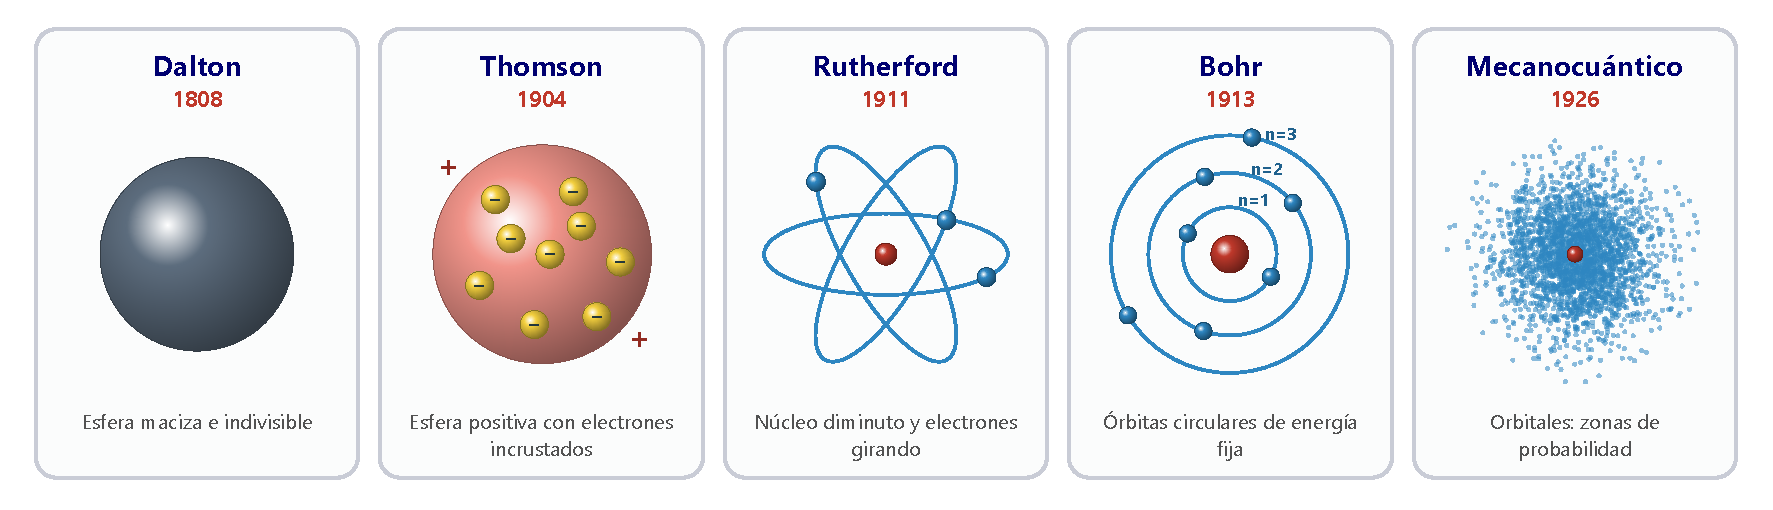
\includegraphics[width=\textwidth]{images/UD3/modelos_atomicos}
    \caption{Evolución de los modelos atómicos.}
    \label{fig:ud3-modelos}
\end{figure}

\subsection{El modelo atómico de Dalton}

Entre 1803 y 1808, \textbf{John Dalton} propuso que los átomos eran \textbf{esferas macizas e indivisibles}, todas iguales
para un mismo elemento y distintas de las de cualquier otro (lo estudiamos en la unidad 1). Este modelo tan sencillo explicaba
las \textbf{leyes ponderales}, pero no contemplaba la existencia de isótopos, predijo mal la fórmula del agua (creyó que era
\ch{HO}) y no podía explicar fenómenos como la electricidad.

\subsection{El descubrimiento del electrón y el modelo de Thomson}

En 1858 se descubrieron los \textbf{rayos catódicos}. Al hacer un vacío casi perfecto en un tubo de vidrio y aplicar una
diferencia de potencial muy alta entre dos electrodos, el \textbf{cátodo} (electrodo negativo) emitía «algo» invisible que
hacía brillar la pared del fondo, recubierta de una sustancia fluorescente. Si se interponía un objeto, su sombra aparecía en la
pantalla: la radiación viajaba en línea recta. En 1897, \textbf{J.\,J. Thomson} estudió a fondo su naturaleza con un tubo como
el de la figura~\ref{fig:ud3-catodicos}.

\begin{figure}[H]
    \centering
    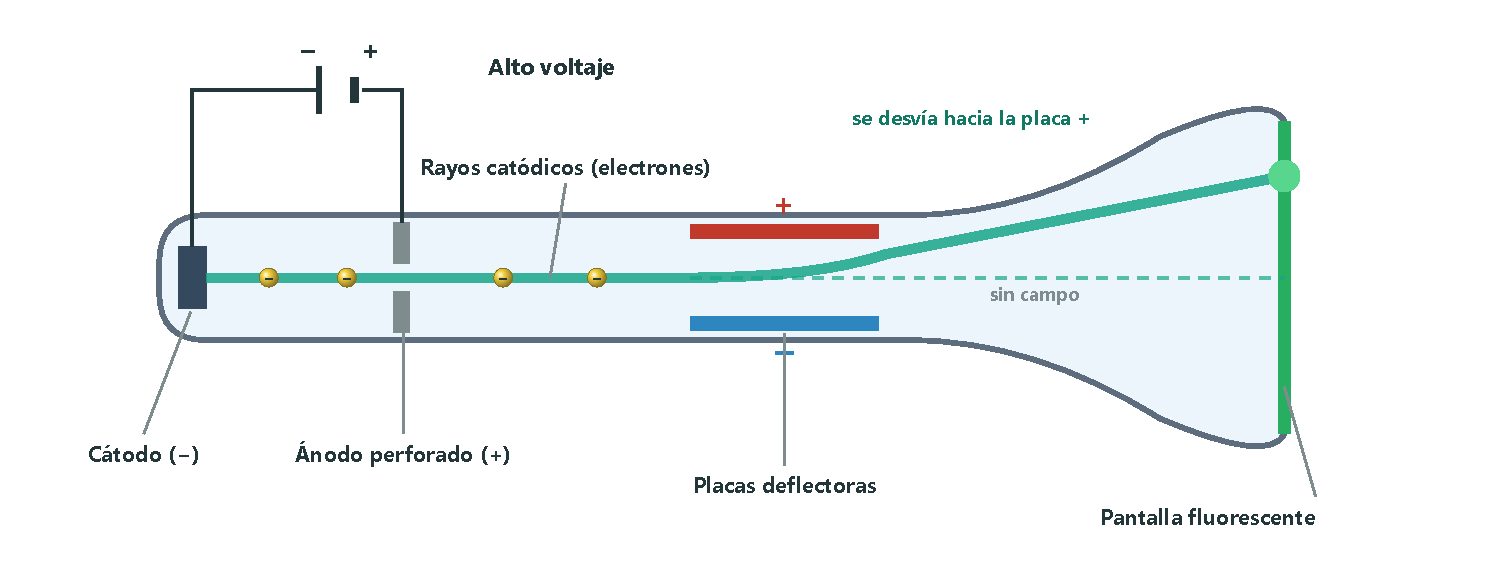
\includegraphics[width=0.85\textwidth]{images/UD3/rayos_catodicos}
    \caption{Tubo de rayos catódicos: las placas cargadas desvían el haz hacia la placa positiva.}
    \label{fig:ud3-catodicos}
\end{figure}

\begin{table}[H]
    \centering
    \caption{Lo que observó Thomson en los rayos catódicos}
    \vspace{-5pt}
    \begin{tabular}{@{}L{7cm}L{7cm}@{}}
        \toprule
        \textbf{Observación} & \textbf{Interpretación} \\
        \midrule
        Hacen girar un pequeño molinillo colocado en su camino & Están formados por \textbf{partículas con masa} \\[3pt]
        Se desvían hacia la placa positiva & Tienen \textbf{carga negativa} \\[3pt]
        Son iguales sea cual sea el metal del cátodo & Son partículas \textbf{fundamentales}, presentes en toda la materia \\[3pt]
        Su relación carga/masa es \(\qty{1.76e11}{\coulomb\per\kilo\gram}\) & Son mucho más \textbf{ligeras} que el átomo más pequeño, el de hidrógeno \\
        \bottomrule
    \end{tabular}
    \label{tab:ud3-thomson}
\end{table}

\begin{definition}[El electrón]
    Thomson concluyó que los rayos catódicos eran partículas con carga negativa, que se llamaron \textbf{electrones}. Su
    existencia demuestra que los átomos \textbf{no son indivisibles}: tienen una estructura interna. Experimentos posteriores
    midieron su carga y su masa:
    \[ q_e = \qty{-1.602e-19}{\coulomb} \qquad\qquad m_e = \qty{9.109e-31}{\kilo\gram} \]
    El electrón no tiene estructura interna: es una \textbf{partícula elemental}.
\end{definition}

En 1909, \textbf{R. Millikan} demostró, con su famoso experimento de la gota de aceite, que cualquier carga eléctrica es un
múltiplo entero de una cantidad mínima, la \textbf{carga elemental}, \(e = \qty{1.602e-19}{\coulomb}\), que es la carga (en
valor absoluto) del electrón.

\paragraph{El modelo de Thomson (1904).} Si los átomos son neutros y contienen electrones, deben tener también carga positiva.
Thomson propuso que el átomo era una \textbf{esfera} con la \textbf{carga positiva repartida uniformemente} en la que estaban
\textbf{incrustados} los electrones, como las pepitas en una sandía. Se le conoce como \emph{modelo del pudin de pasas}. Thomson
recibió el premio Nobel de Física en 1906 por sus investigaciones sobre la conducción de la electricidad en los gases.

\begin{example}
    \textbf{La carga está cuantizada.} En un experimento como el de Millikan se miden las cargas de tres gotas de aceite:
    \(\qty{3.204e-19}{\coulomb}\), \(\qty{4.806e-19}{\coulomb}\) y \(\qty{8.010e-19}{\coulomb}\). ¿Cuántos electrones de exceso
    tiene cada gota?

    \textbf{Solución.} Dividimos cada carga entre la carga elemental:
    \[ \frac{\num{3.204e-19}}{\num{1.602e-19}} = 2; \qquad \frac{\num{4.806e-19}}{\num{1.602e-19}} = 3; \qquad \frac{\num{8.010e-19}}{\num{1.602e-19}} = 5 \]
    Las gotas tienen 2, 3 y 5 electrones de exceso. Nunca se encuentra una carga que no sea un múltiplo entero de \(e\).
\end{example}

\subsection{El modelo atómico de Rutherford}

\paragraph{El experimento de la lámina de oro.} En 1910, \textbf{E. Rutherford} y sus colaboradores \textbf{H. Geiger} y
\textbf{E. Marsden} pusieron a prueba el modelo de Thomson bombardeando una lámina de oro finísima (de una micra de espesor, unas
mil capas de átomos) con \textbf{partículas \(\alpha\)}, de masa \qty{4}{\uma} y carga \(+2e\). Si el modelo de Thomson era
correcto, la masa y la carga estarían repartidas por todo el átomo, como un fluido de muy poca densidad, y las partículas
\(\alpha\), muy rápidas, deberían atravesar la lámina casi sin desviarse. Lo que encontraron fue sorprendente
(figura~\ref{fig:ud3-oro}): casi todas pasaban sin desviarse, pero alrededor de \textbf{una de cada \num{20000} se desviaba más
de \ang{90}}, ¡e incluso alguna rebotaba! Rutherford lo comparó con disparar un proyectil contra una hoja de papel de seda y que
volviera hacia atrás.

\begin{figure}[H]
    \centering
    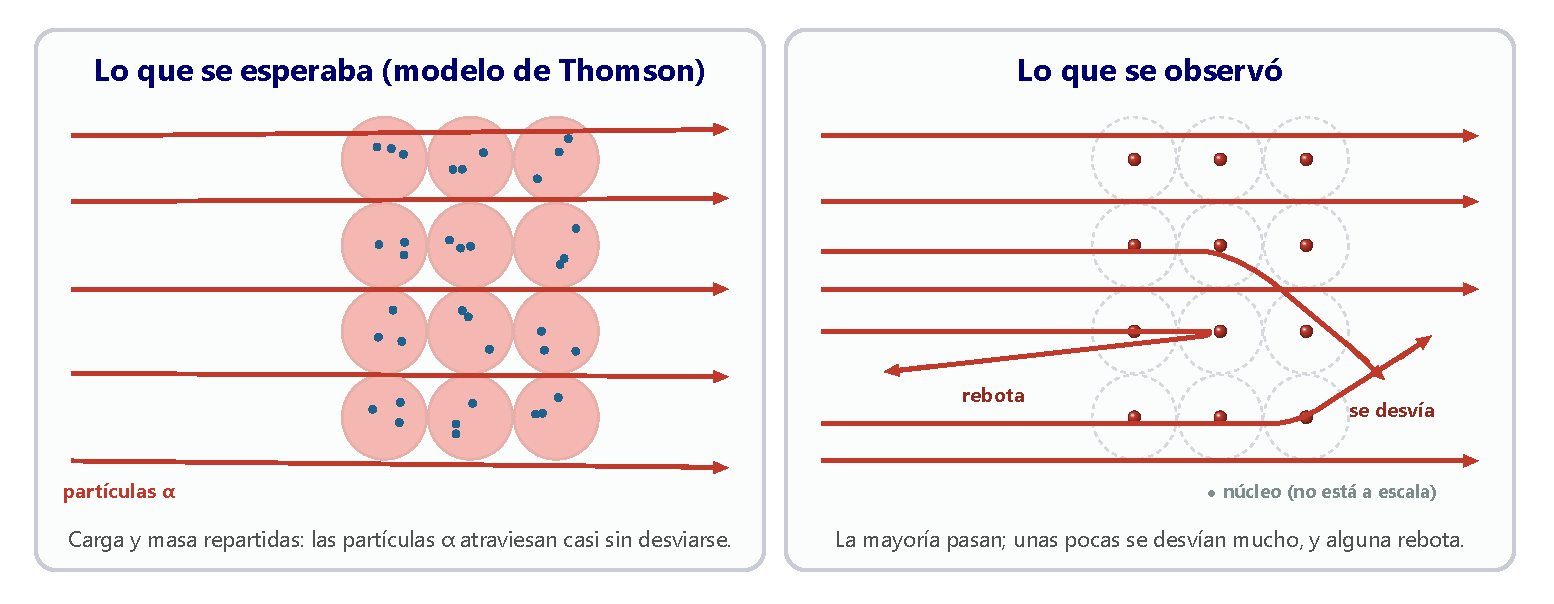
\includegraphics[width=0.9\textwidth]{images/UD3/lamina_oro}
    \caption{Experimento de la lámina de oro: lo que se esperaba y lo que se observó.}
    \label{fig:ud3-oro}
\end{figure}

Rutherford interpretó que en el interior del átomo tenía que haber una zona muy \textbf{densa} y con carga \textbf{positiva},
capaz de repeler y hacer rebotar a las partículas \(\alpha\) que chocaban con ella. Como eso ocurría muy pocas veces, esa zona
debía ser \textbf{pequeñísima} comparada con el átomo.

\begin{definition}[Modelo atómico de Rutherford (1911)]
    \leavevmode % el título de la definición en su propia línea, la lista debajo
    \begin{itemize}
        \item La mayor parte del volumen del átomo está \textbf{vacío}.
        \item En el centro hay un \textbf{núcleo} muy pequeño en el que se concentra casi toda la \textbf{masa} y toda la
        \textbf{carga positiva}.
        \item Los \textbf{electrones} están en la zona exterior, la \textbf{corteza}, \textbf{girando} alrededor del núcleo en
        órbitas circulares, lo que explica que no caigan sobre él a pesar de la atracción eléctrica.
    \end{itemize}
    Por su parecido con el sistema solar se le llama \emph{modelo planetario}.
\end{definition}

\begin{remark}
    \textbf{Un átomo casi vacío.} El radio de un átomo es unas \num{100000} veces mayor que el de su núcleo. Si el núcleo fuera un
    guisante en el centro de un campo de fútbol, los electrones estarían dando vueltas por las gradas.
\end{remark}

\paragraph{El protón.} Ya en 1886 \textbf{E. Goldstein} había detectado rayos con carga positiva en los tubos de descarga, pero
su trabajo tuvo poca repercusión. En 1919, Rutherford obtuvo núcleos de hidrógeno al bombardear nitrógeno con partículas
\(\alpha\), y propuso que el núcleo de hidrógeno, el más pequeño, era una sola partícula con carga positiva, a la que llamó
\textbf{protón}, y que todos los núcleos contenían cierto número de protones:
\(q_p = +e = \qty{1.602e-19}{\coulomb}\) y \(m_p = \qty{1.673e-27}{\kilo\gram}\).

\paragraph{El neutrón.} La masa de los núcleos era mayor que la de sus protones, y además los protones se repelen entre sí. Por
eso Rutherford propuso que en el núcleo había también partículas \textbf{sin carga} y \textbf{con masa}, que lo hicieran estable.
En 1932, \textbf{J. Chadwick} las detectó: era el \textbf{neutrón}, de masa \(m_n = \qty{1.675e-27}{\kilo\gram}\).

\begin{table}[H]
    \centering
    \caption{Partículas subatómicas}
    \vspace{-5pt}
    \begin{tabular}{@{}lccccc@{}}
        \toprule
        \textbf{Partícula} & \textbf{Masa (kg)} & \textbf{Masa (u)} & \textbf{Carga (C)} & \makecell{\textbf{Carga} \\ \textbf{relativa}} & \textbf{Localización} \\
        \midrule
        Electrón, \(e^-\) & \num{9.109e-31} & \num{0.00055} & \num{-1.602e-19} & \(-1\) & Corteza \\[3pt]
        Protón, \(p^+\) & \num{1.673e-27} & \num{1.0073} & \num{+1.602e-19} & \(+1\) & Núcleo \\[3pt]
        Neutrón, \(n\) & \num{1.675e-27} & \num{1.0087} & 0 & 0 & Núcleo \\
        \bottomrule
    \end{tabular}
    \label{tab:ud3-particulas}
\end{table}

\paragraph{Limitaciones del modelo de Rutherford.} El modelo nuclear fue un gran avance (el modelo actual conserva la idea de
núcleo), pero pronto se vieron sus fallos:
\begin{itemize}
    \item Según la física clásica, una carga eléctrica que gira emite radiación y pierde energía. Los electrones irían cayendo en
    espiral hasta chocar con el núcleo: el átomo sería \textbf{inestable}. Sin embargo, la materia es estable.
    \item Los átomos podrían absorber o emitir cualquier cantidad de energía, pero, como veremos, sus espectros son
    \textbf{discontinuos}.
\end{itemize}

\begin{exercise}
    Imagina que lanzas cientos de pelotas de tenis contra una gran cortina y casi todas la atraviesan, pero unas pocas salen
    rebotadas hacia ti. ¿Qué pensarías que hay detrás de la cortina? ¿Qué experimento de la historia de la química se parece a
    esta situación?
    \begin{solu}
        \textcolor{red}{Que detrás hay algunos objetos pequeños y muy duros o pesados} (postes, piedras) y mucho espacio vacío entre
        ellos. Se parece al \textcolor{red}{experimento de la lámina de oro de Rutherford}: las partículas \(\alpha\) que rebotan
        delatan la existencia de un núcleo pequeño, denso y positivo.
    \end{solu}
\end{exercise}

\begin{exercise}
    Imagina que eres uno de los científicos del experimento de la lámina de oro. Al ver los resultados, ¿qué modelo atómico
    propondrías? ¿En qué se diferencia del de Thomson?
    \begin{solu}
        \textcolor{red}{Un modelo con un núcleo central diminuto, positivo y con casi toda la masa, y los electrones fuera, en un
        espacio casi vacío.} En el modelo de Thomson la carga positiva y la masa están repartidas por todo el átomo y los electrones
        están incrustados en ella; en el de Rutherford están separadas en núcleo y corteza.
    \end{solu}
\end{exercise}

\begin{exercise}
    Siempre se habla de Rutherford al mencionar el experimento de la lámina de oro, pero hubo otros científicos que trabajaron con
    él. Investiga quiénes eran y qué otros logros consiguieron, y prepara una infografía.
    \begin{solu}
        \textcolor{red}{Hans Geiger y Ernest Marsden.} \textcolor{blue}{Geiger inventó, con sus alumnos, el contador de radiación
        que lleva su nombre y estudió la relación entre la energía de las partículas \(\alpha\) y la vida media de los núcleos
        radiactivos (ley de Geiger-Nuttall). Marsden, que era todavía estudiante cuando hizo el experimento, se trasladó a Nueva
        Zelanda, donde investigó en física aplicada a la agricultura, y durante la Segunda Guerra Mundial colaboró en el desarrollo
        del radar.}
    \end{solu}
\end{exercise}

\begin{exercise}
    a) Calcula la relación carga/masa del electrón y la del protón. b) ¿Cuántas veces es mayor la masa del protón que la del
    electrón? ¿Por qué decimos que la masa del átomo está en el núcleo?
    \begin{solu}
        a) \(\dfrac{e}{m_e} = \dfrac{\num{1.602e-19}}{\num{9.109e-31}} = \textcolor{red}{\qty{1.76e11}{\coulomb\per\kilo\gram}}\);
        \(\dfrac{e}{m_p} = \dfrac{\num{1.602e-19}}{\num{1.673e-27}} = \textcolor{red}{\qty{9.58e7}{\coulomb\per\kilo\gram}}\).
        b) \(\dfrac{m_p}{m_e} = \textcolor{red}{1837}\). \textcolor{blue}{Protones y neutrones tienen casi 2000 veces más masa que
        los electrones, y están todos en el núcleo.}
    \end{solu}
\end{exercise}

\begin{exercise}
    El radio de un átomo es unas \(10^5\) veces mayor que el de su núcleo. Si hiciéramos una maqueta en la que el núcleo fuera
    una canica de \qty{1}{\cm} de diámetro, ¿qué diámetro tendría el átomo?
    \begin{solu}
        \(\qty{1}{\cm} \cdot 10^5 = \qty{e5}{\cm} = \textcolor{red}{\qty{1}{\km}}\): el átomo sería una esfera de un kilómetro de
        diámetro con una canica en el centro.
    \end{solu}
\end{exercise}

\begin{exercise}
    «Los científicos no dependen de las ideas de un solo hombre, sino de la sabiduría combinada de miles de hombres…», escribió
    Rutherford. ¿Sigue siendo válida esta idea hoy? ¿Por qué es importante colaborar en la investigación científica?
    \begin{solu}
        \textcolor{red}{Respuesta abierta.} \textcolor{blue}{Hoy la ciencia es aún más colaborativa: los grandes avances
        (el bosón de Higgs, las vacunas de ARN, el telescopio James Webb) los firman equipos de cientos o miles de personas de
        muchos países. Cada modelo atómico se apoyó en experimentos y en ideas de otros, como se ve en esta unidad. Hoy diríamos
        «personas», no solo «hombres».}
    \end{solu}
\end{exercise}

\begin{exercise}
    En la historia de los modelos atómicos se mencionan muy pocas mujeres. ¿A qué crees que se debe? Investiga la contribución de
    alguna de ellas, como Harriet Brooks, Marie Curie o Lise Meitner, y escribe un breve informe.
    \begin{solu}
        \textcolor{red}{Respuesta abierta.} \textcolor{blue}{Durante mucho tiempo las mujeres tuvieron muy difícil estudiar en la
        universidad y trabajar en investigación, y su trabajo se atribuía a menudo a sus compañeros. Harriet Brooks, primera mujer
        que trabajó con Rutherford, descubrió el retroceso nuclear y el radón; Marie Curie estudió la radiactividad y descubrió el
        polonio y el radio; Lise Meitner explicó, junto con Otto Frisch, la fisión nuclear.}
    \end{solu}
\end{exercise}

%========================================================================================
\section{La masa de los átomos}\label{sec:ud3-masa}
%========================================================================================

\subsection{Número atómico y número másico}

\begin{definition}[Número atómico y número másico]
    \leavevmode % el título de la definición en su propia línea, la lista debajo
    \begin{itemize}
        \item El \textbf{número atómico}, \(Z\), es el número de \textbf{protones} del núcleo. Todos los átomos con el mismo
        número atómico tienen las mismas propiedades químicas: un \textbf{elemento químico} es una sustancia formada por átomos con
        el mismo \(Z\).
        \item El \textbf{número másico}, \(A\), es el número de \textbf{nucleones} (protones más neutrones) del núcleo:
        \[ A = Z + N \qquad (N = \text{número de neutrones}) \]
    \end{itemize}
    Un átomo se representa \(^{A}_{Z}\mathrm{X}\), donde X es el símbolo del elemento; si es un ion, su carga neta se escribe
    arriba a la derecha.
\end{definition}

\begin{example}
    \textbf{Partículas de un átomo.} Indica el número másico, el número atómico y el número de protones, neutrones y electrones
    del isótopo \ch{^{238}_{92}U}.

    \textbf{Solución.} De la notación leemos directamente \(Z = 92\) y \(A = 238\). El número de protones es el número atómico:
    \(p = 92\). Los neutrones: \(N = A - Z = 238 - 92 = 146\). Como el átomo es neutro, tiene tantos electrones como protones:
    92 electrones.
\end{example}

\subsection{Isótopos}

\begin{definition}[Isótopos]
    Son átomos de un mismo elemento (igual número de \textbf{protones}) con distinto número de \textbf{neutrones}, es decir,
    con el mismo \(Z\) y distinto \(A\). La palabra viene del griego \emph{isos}, «igual», y \emph{topos}, «lugar»: ocupan el
    mismo lugar en la tabla periódica.
\end{definition}

La mayoría de los elementos naturales son mezclas de varios isótopos. Como tienen los mismos electrones, su comportamiento
químico es el mismo, aunque algunas propiedades físicas (la masa, la densidad, la estabilidad del núcleo) son distintas. El
oxígeno, por ejemplo, tiene tres isótopos estables: \ch{^{16}_{8}O}, \ch{^{17}_{8}O} y \ch{^{18}_{8}O}; el hidrógeno tiene los
tres de la figura~\ref{fig:ud3-isotopos}. La \textbf{abundancia isotópica} es el porcentaje de átomos de un isótopo que hay en
una muestra natural del elemento.

\begin{figure}[H]
    \centering
    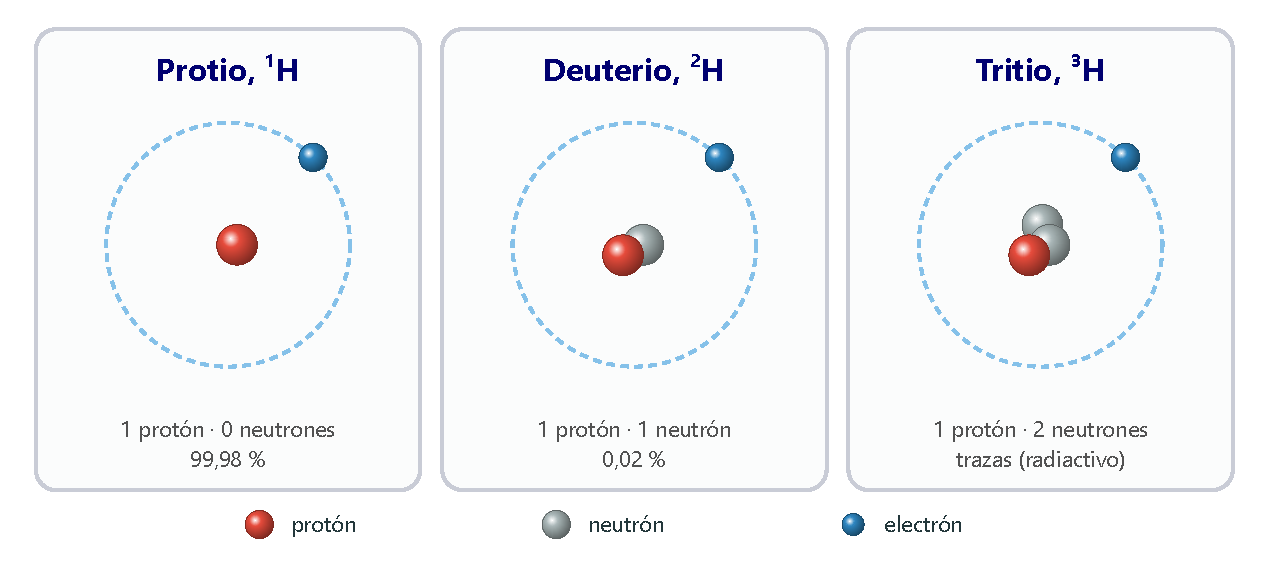
\includegraphics[width=0.72\textwidth]{images/UD3/isotopos}
    \caption{Los tres isótopos del hidrógeno (el núcleo no está a escala).}
    \label{fig:ud3-isotopos}
\end{figure}

\begin{exercise}
    Indica el número de protones, neutrones y electrones de: \ch{^{119}_{50}Sn^4+}, \ch{^{37}_{17}Cl^-}, \ch{^{107}_{47}Ag^+},
    \ch{^{59}_{27}Co^2+} y \ch{^{238}_{92}U}.
    \begin{solu}
        \begin{tabular}{@{}lccccc@{}}
            \toprule
            & \ch{^{119}_{50}Sn^4+} & \ch{^{37}_{17}Cl^-} & \ch{^{107}_{47}Ag^+} & \ch{^{59}_{27}Co^2+} & \ch{^{238}_{92}U} \\
            \midrule
            Protones & 50 & 17 & 47 & 27 & 92 \\[3pt]
            Neutrones & 69 & 20 & 60 & 32 & 146 \\[3pt]
            Electrones & \textcolor{red}{46} & \textcolor{red}{18} & \textcolor{red}{46} & \textcolor{red}{25} & \textcolor{red}{92} \\
            \bottomrule
        \end{tabular}
    \end{solu}
\end{exercise}

\begin{exercise}
    De los átomos \ch{^{12}_{6}C}, \ch{^{14}_{6}C}, \ch{^{14}_{7}N}, \ch{^{40}_{18}Ar} y \ch{^{40}_{20}Ca}, ¿cuáles son isótopos
    entre sí? ¿Cuáles tienen el mismo número másico? ¿Cuáles tienen el mismo número de neutrones?
    \begin{solu}
        \textcolor{red}{Isótopos: \ch{^{12}C} y \ch{^{14}C}} (mismo \(Z\)). \textcolor{red}{Mismo \(A\): \ch{^{14}C} y \ch{^{14}N};
        \ch{^{40}Ar} y \ch{^{40}Ca}.} Neutrones: 6, 8, 7, 22 y 20: \textcolor{red}{ninguno coincide}.
    \end{solu}
\end{exercise}

\subsection{La masa atómica}

La masa atómica de un elemento se calcula con mucha precisión a partir de su \textbf{espectro de masas}.

\paragraph{Espectrometría de masas.} Es una técnica de análisis que permite \textbf{separar las partículas} de una muestra
(átomos, moléculas o fragmentos de moléculas) \textbf{según su masa}. Un \textbf{espectrómetro de masas}
(figura~\ref{fig:ud3-espectrometro}) tiene tres partes:
\begin{itemize}
    \item \textbf{Fuente de iones}: la muestra, en estado gaseoso, se \textbf{ioniza}; normalmente todos los iones adquieren la
    misma carga. Después, unas placas cargadas los aceleran.
    \item \textbf{Analizador}: los iones atraviesan un \textbf{campo magnético} que curva su trayectoria. El radio de la curva
    depende de la masa de cada ion: los más ligeros se desvían más. Así, el haz inicial se \textbf{separa} en tantos haces como
    masas distintas había en la muestra.
    \item \textbf{Detector}: recoge cada haz por separado y mide el \textbf{número de iones} que llegan.
\end{itemize}

\begin{figure}[H]
    \centering
    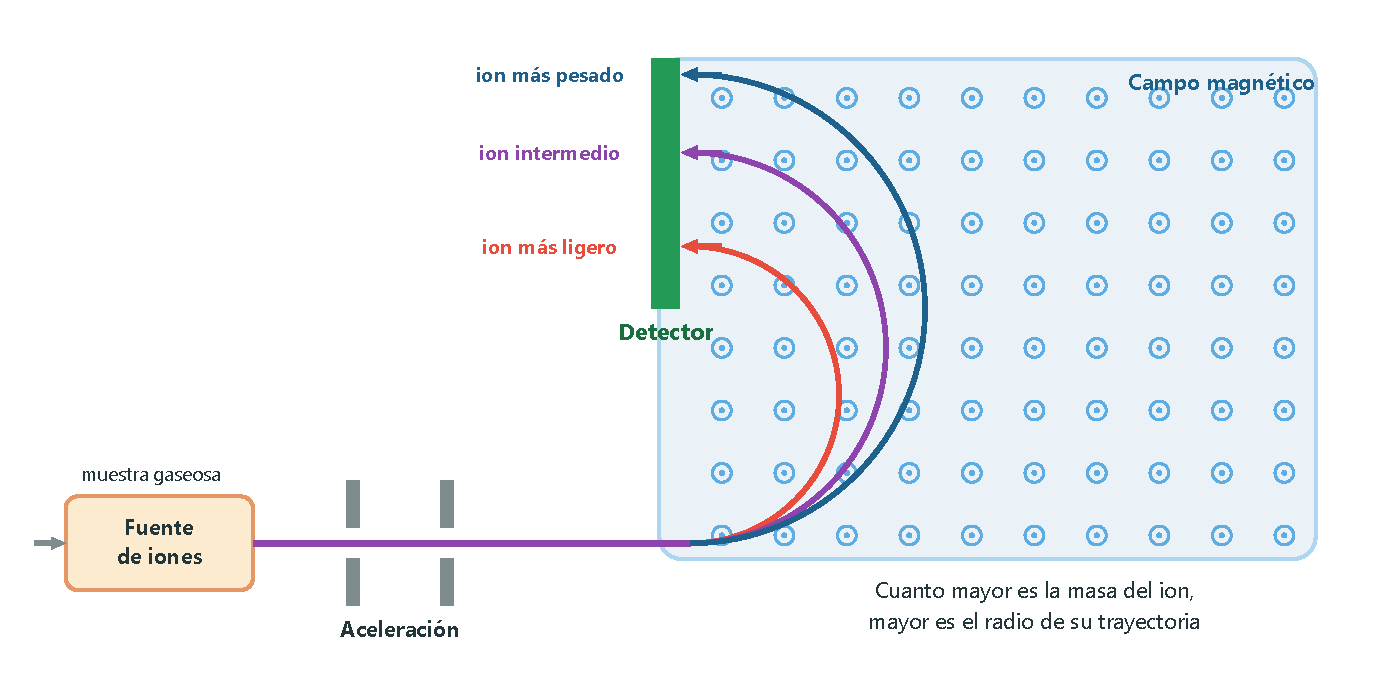
\includegraphics[width=0.7\textwidth]{images/UD3/espectrometro}
    \caption{Esquema de un espectrómetro de masas.}
    \label{fig:ud3-espectrometro}
\end{figure}

El resultado es el \textbf{espectro de masas} (figura~\ref{fig:ud3-espectro-cl}): cada pico indica la \textbf{masa} de un tipo
de partícula y su altura, la \textbf{abundancia relativa} (el porcentaje de cada partícula en la muestra).

\begin{figure}[H]
    \centering
    \begin{tikzpicture}
        \begin{axis}[grafica, width=0.55\linewidth, height=5cm, ybar, bar width=5pt, xmin=33.5, xmax=38.5, ymin=0, ymax=90,
            xtick={34,35,36,37,38}, xlabel={Masa isotópica (u)}, ylabel={Abundancia (\%)}, grid=none,
            nodes near coords, nodes near coords style={font=\scriptsize, /pgf/number format/use comma}]
            \addplot[fill=ocre!70, draw=ocre] coordinates {(34.969,75.78) (36.966,24.22)};
        \end{axis}
    \end{tikzpicture}
    \caption{Espectro de masas del cloro: dos isótopos, \ch{^{35}Cl} y \ch{^{37}Cl}.}
    \label{fig:ud3-espectro-cl}
\end{figure}

\begin{definition}[Masa atómica de un elemento]
    Es la \textbf{media ponderada} de las masas de sus isótopos, según su abundancia:
    \[ \bar{A} = \frac{\sum A_i \cdot \%_i}{100} = \frac{A_1 \cdot \%_1 + A_2 \cdot \%_2 + \dots}{100} \]
    donde \(A_i\) es la masa del isótopo \(i\) (en u) y \(\%_i\), su abundancia relativa. Por eso las masas atómicas de la tabla
    periódica no son números enteros.
\end{definition}

\begin{example}
    \textbf{Masa atómica del silicio.} El silicio natural está formado por \ch{^{28}Si} (\qty{27.977}{\uma}; 92,2\,\%),
    \ch{^{29}Si} (\qty{28.976}{\uma}; 4,7\,\%) y \ch{^{30}Si} (\qty{29.974}{\uma}). Calcula su masa atómica.

    \textbf{Solución.} Primero, la abundancia que falta: \(100 - (\num{92.2} + \num{4.7}) = \qty{3.1}{\percent}\) de \ch{^{30}Si}.
    \[ \bar{A} = \frac{\num{27.977} \cdot \num{92.2} + \num{28.976} \cdot \num{4.7} + \num{29.974} \cdot \num{3.1}}{100} = \qty{28.09}{\uma} \]
    El resultado está muy cerca de 28, porque casi todo el silicio es \ch{^{28}Si}.
\end{example}

\begin{example}
    \textbf{Abundancias a partir de la masa atómica.} El boro tiene dos isótopos, \ch{^{10}B} (\qty{10.013}{\uma}) y \ch{^{11}B}
    (\qty{11.009}{\uma}), y su masa atómica es \qty{10.81}{\uma}. Calcula la abundancia de cada uno.

    \textbf{Solución.} Si \(x\) es el porcentaje de \ch{^{10}B}, el de \ch{^{11}B} es \(100 - x\):
    \[ \num{10.81} = \frac{\num{10.013}\,x + \num{11.009}\,(100 - x)}{100} \;\Rightarrow\; 1081 = 1100{,}9 - \num{0.996}\,x
    \;\Rightarrow\; x = \num{19.98} \]
    Hay un 20,0\,\% de \ch{^{10}B} y un 80,0\,\% de \ch{^{11}B}.
\end{example}

\begin{exercise}
    El galio tiene dos isótopos: \ch{^{69}Ga}, de \qty{68.926}{\uma} y 60,11\,\% de abundancia, y \ch{^{71}Ga}, de
    \qty{70.925}{\uma} y 39,89\,\%. Calcula la masa atómica del galio y dibuja su espectro de masas.
    \begin{solu}
        \(\bar{A} = \dfrac{\num{68.926} \cdot \num{60.11} + \num{70.925} \cdot \num{39.89}}{100} = \textcolor{red}{\qty{69.72}{\uma}}\).
        \textcolor{blue}{El espectro tiene dos picos, en 68,9 y en 70,9, de alturas 60,11 y 39,89.}
    \end{solu}
\end{exercise}

\begin{exercise}
    Calcula la masa atómica de: a) el cobre: \ch{^{63}Cu}, \qty{62.93}{\uma}, 69,17\,\%; \ch{^{65}Cu}, \qty{64.93}{\uma},
    30,83\,\%; b) el cloro, con los datos de la figura~\ref{fig:ud3-espectro-cl}.
    \begin{solu}
        a) \(\dfrac{\num{62.93} \cdot \num{69.17} + \num{64.93} \cdot \num{30.83}}{100} = \textcolor{red}{\qty{63.55}{\uma}}\).
        b) \(\dfrac{\num{34.969} \cdot \num{75.78} + \num{36.966} \cdot \num{24.22}}{100} = \textcolor{red}{\qty{35.45}{\uma}}\).
    \end{solu}
\end{exercise}

\begin{exercise}
    El argón tiene tres isótopos estables: \ch{^{36}Ar} (\qty{35.968}{\uma}; 0,337\,\%), \ch{^{38}Ar} (\qty{37.963}{\uma};
    0,063\,\%) y \ch{^{40}Ar} (\qty{39.962}{\uma}; 99,600\,\%). Calcula su masa atómica. ¿Por qué el argón (\(Z = 18\)) tiene
    mayor masa atómica que el potasio (\(Z = 19\), \qty{39.10}{\uma})?
    \begin{solu}
        \(\bar{A} = \dfrac{\num{35.968} \cdot \num{0.337} + \num{37.963} \cdot \num{0.063} + \num{39.962} \cdot \num{99.600}}{100} =
        \textcolor{red}{\qty{39.95}{\uma}}\). \textcolor{red}{Porque el isótopo más abundante del argón tiene 22 neutrones}, y el
        del potasio (\ch{^{39}K}), solo 20. La masa no depende solo de \(Z\): por eso la tabla se ordena por número atómico y no por
        masa.
    \end{solu}
\end{exercise}

%========================================================================================
\section{Interacción de la radiación electromagnética con la materia}\label{sec:ud3-radiacion}
%========================================================================================

La forma en que la luz y las demás ondas electromagnéticas interaccionan con la materia nos da mucha información sobre la
estructura interna de los átomos. Veamos primero qué son estas ondas.

\subsection{Ondas electromagnéticas}

En el siglo XIX hubo una larga discusión sobre si la luz era un haz de partículas o una onda, que pareció zanjarse a favor de la
teoría ondulatoria. En 1865, \textbf{J.\,C. Maxwell} demostró teóricamente que un campo eléctrico y uno magnético acoplados se
propagan en forma de \textbf{onda}, incluso en el \textbf{vacío}, a unos \qty{300000}{\km\per\s}: la velocidad de la luz. Las
\textbf{ondas electromagnéticas} transportan energía mediante la variación sinusoidal de un campo eléctrico y otro magnético
perpendiculares. En 1887, \textbf{H. Hertz} las generó y las detectó en el laboratorio, confirmando las predicciones de Maxwell.

\begin{figure}[H]
    \centering
    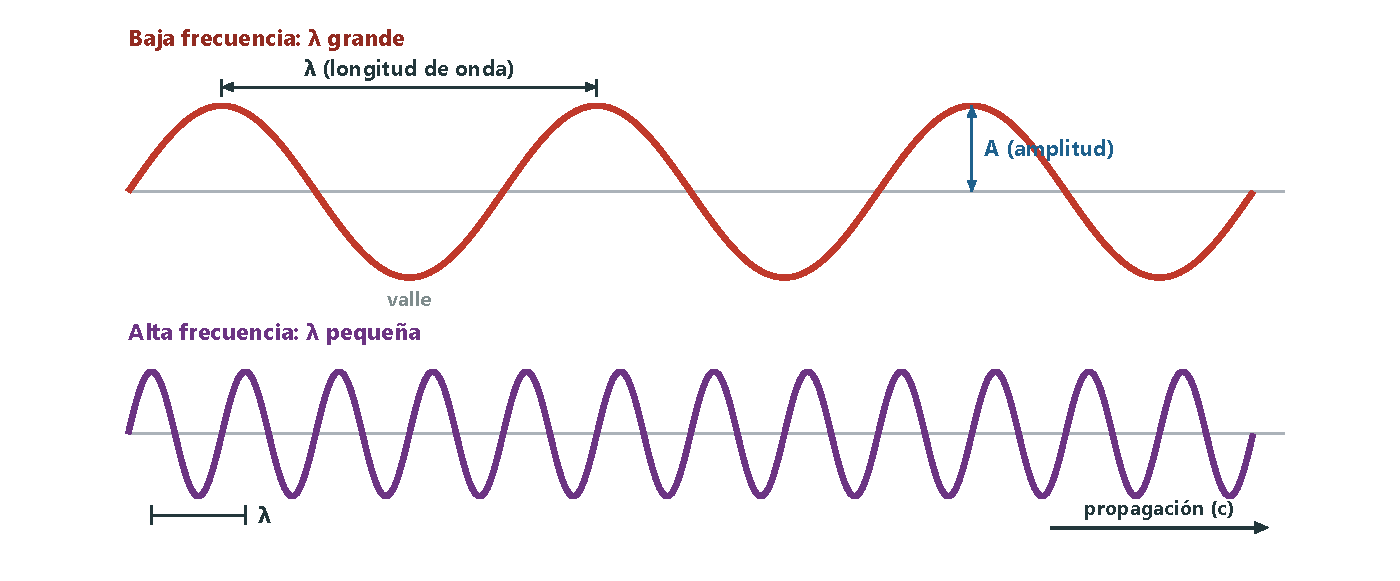
\includegraphics[width=0.7\textwidth]{images/UD3/onda}
    \caption{Longitud de onda y amplitud de una onda. Cuanto mayor es la frecuencia, menor es la longitud de onda.}
    \label{fig:ud3-onda}
\end{figure}

\begin{table}[H]
    \centering
    \caption{Magnitudes de una onda}
    \vspace{-5pt}
    \begin{tabular}{@{}lcL{8.2cm}@{}}
        \toprule
        \textbf{Magnitud} & \makecell{\textbf{Símbolo} \\ \textbf{(unidad SI)}} & \textbf{Significado} \\
        \midrule
        Longitud de onda & \(\lambda\) (\unit{\m}) & Distancia entre dos crestas consecutivas \\[3pt]
        Periodo & \(T\) (\unit{\s}) & Tiempo que tarda la onda en avanzar una longitud de onda \\[3pt]
        Frecuencia & \(\nu\) (\unit{\hertz} = \unit{\per\s}) & Número de ondas que pasan por un punto en cada segundo (hercio, en honor a Hertz) \\[3pt]
        Número de onda & \(\tilde{\nu}\) (\unit{\per\m}) & Número de longitudes de onda que caben en una unidad de longitud \\[3pt]
        Velocidad de propagación & \(c\) (\unit{\m\per\s}) & Distancia que avanza la onda en cada segundo; en el vacío, \(c = \qty{3.00e8}{\m\per\s}\) \\
        \bottomrule
    \end{tabular}
    \label{tab:ud3-magnitudes}
\end{table}

Estas magnitudes están relacionadas:
\[ \nu = \frac{1}{T} \qquad\qquad \tilde{\nu} = \frac{1}{\lambda} \qquad\qquad c = \frac{\lambda}{T} = \lambda \cdot \nu \]

\begin{example}
    \textbf{Televisión UHF.} Las antiguas televisiones sintonizaban la banda UHF, que ocupa frecuencias entre 300 MHz y 3 GHz.
    ¿Qué longitud de onda tiene una emisión de \qty{600}{\mega\hertz}?

    \textbf{Solución.} \(\lambda = \dfrac{c}{\nu} = \dfrac{\qty{3.00e8}{\m\per\s}}{\qty{600e6}{\hertz}} = \qty{0.500}{\m} = \qty{50.0}{\cm}\).
\end{example}

\subsection{El espectro electromagnético}

\begin{definition}[Espectro electromagnético]
    Es el conjunto de todas las ondas electromagnéticas, ordenadas según su frecuencia o su longitud de onda. La
    \textbf{energía} que transporta una onda es tanto mayor cuanto mayor es su \textbf{frecuencia} (y menor su longitud de onda).
\end{definition}

La \textbf{luz visible} es solo una pequeña parte del espectro, con longitudes de onda entre unos \qty{380}{\nm} (violeta) y
\qty{750}{\nm} (rojo) (figura~\ref{fig:ud3-espectro-em}). Las radiaciones más energéticas que el visible (ultravioleta, rayos X
y gamma) pueden arrancar electrones a los átomos: son \textbf{ionizantes}, y por eso peligrosas para los seres vivos.

\begin{figure}[H]
    \centering
    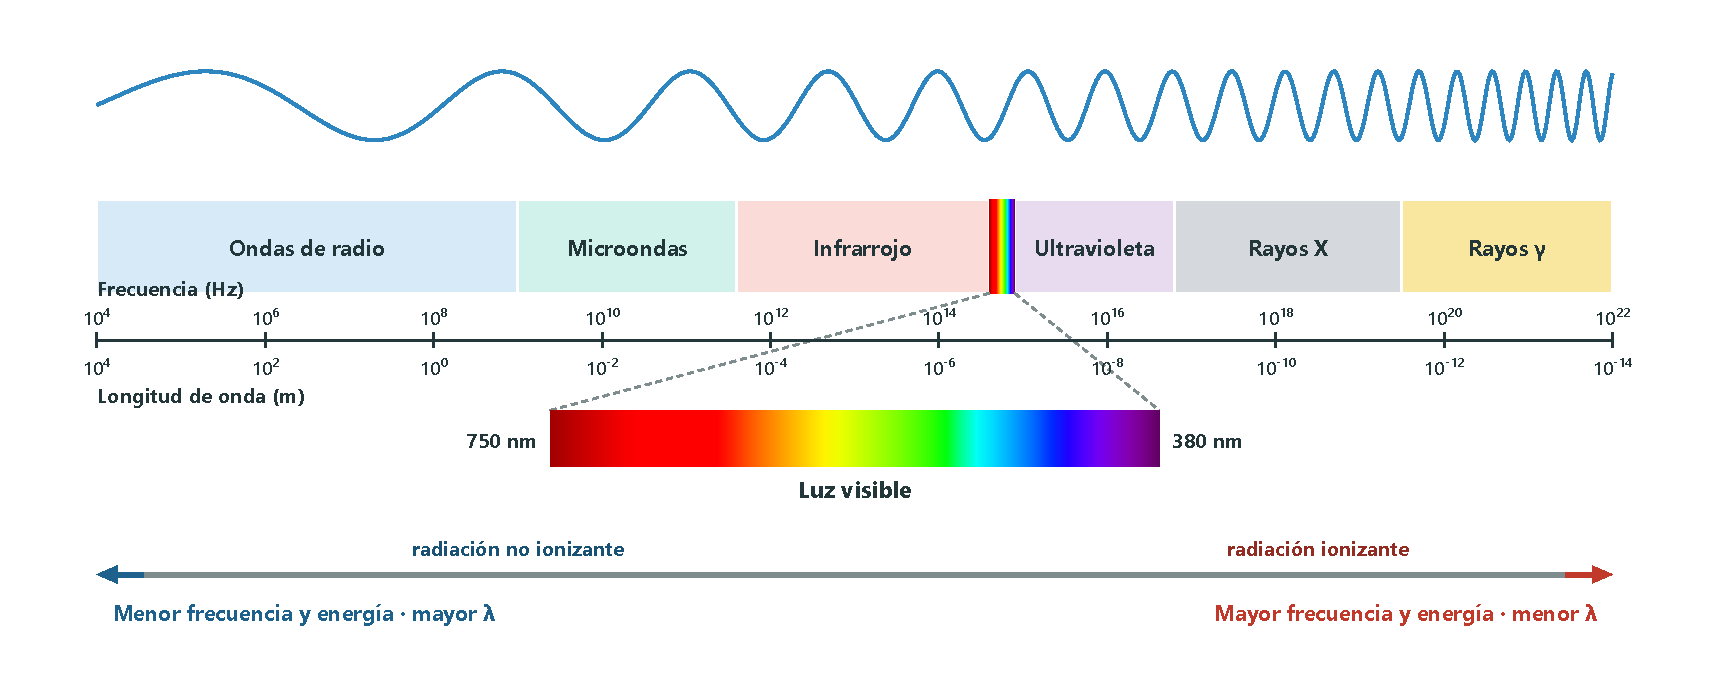
\includegraphics[width=\textwidth]{images/UD3/espectro_em}
    \caption{El espectro electromagnético.}
    \label{fig:ud3-espectro-em}
\end{figure}

\begin{exercise}
    Un teléfono móvil emite y recibe una señal de \qty{900}{\mega\hertz}. ¿Cuál es su longitud de onda?
    \begin{solu}
        \(\lambda = \dfrac{\num{3.00e8}}{\num{9.00e8}} = \textcolor{red}{\qty{0.333}{\m} = \qty{33.3}{\cm}}\).
    \end{solu}
\end{exercise}

\begin{exercise}
    Al pasar un haz de luz blanca por un prisma se descompone en los colores del arcoíris. ¿Por qué se llama a esa zona
    \emph{espectro visible}? Calcula su intervalo de frecuencias.
    \begin{solu}
        \textcolor{red}{Porque es la única parte del espectro que detecta el ojo humano.} \(\nu = c/\lambda\):
        \(\dfrac{\num{3.00e8}}{\num{750e-9}} = \qty{4.0e14}{\hertz}\) (rojo) y \(\dfrac{\num{3.00e8}}{\num{380e-9}} = \qty{7.9e14}{\hertz}\)
        (violeta): \textcolor{red}{entre \num{4.0e14} y \qty{7.9e14}{\hertz}}.
    \end{solu}
\end{exercise}

\begin{exercise}
    ¿Es correcto decir que la luz infrarroja es visible? ¿Cómo es posible entonces que las cámaras térmicas «vean» a las personas
    en la oscuridad?
    \begin{solu}
        \textcolor{red}{No: su longitud de onda es mayor que la del rojo y nuestro ojo no la detecta.} Todos los cuerpos emiten
        radiación infrarroja según su temperatura; \textcolor{red}{las cámaras térmicas tienen sensores sensibles al infrarrojo} y
        la convierten en una imagen visible.
    \end{solu}
\end{exercise}

\subsection{Espectros atómicos}

La materia \textbf{absorbe} radiación, y el efecto que produce depende de la frecuencia y del tipo de materia: las moléculas de
agua de los alimentos absorben microondas y se agitan, y el rozamiento con las moléculas cercanas calienta la comida. La materia
también \textbf{emite} radiación, con una frecuencia que depende de la temperatura: el filamento de las antiguas bombillas,
muy caliente, emitía luz visible.

En 1859, \textbf{R. Bunsen} y \textbf{G. Kirchhoff} idearon el \textbf{espectroscopio}, un aparato que separa, con un prisma o
una red de difracción, las radiaciones de distinta frecuencia que forman un haz.
\begin{itemize}
    \item En la \textbf{espectroscopía de absorción} se hace pasar luz blanca a través de una muestra gaseosa y se analiza la luz
    que sale: se obtiene el \textbf{espectro de absorción}.
    \item En la \textbf{espectroscopía de emisión} se analiza la radiación que emite una sustancia excitada (calentada o sometida a
    una descarga eléctrica): es su \textbf{espectro de emisión}.
\end{itemize}

Con el modelo de Rutherford no había ninguna limitación para la energía del electrón, así que se esperaba que los espectros
fueran \textbf{continuos}: que los átomos absorbieran o emitieran radiación de todas las frecuencias. No es así: los espectros
atómicos son \textbf{discontinuos}. Los átomos solo absorben unas frecuencias determinadas, que aparecen como rayas negras en el
espectro de absorción, y al excitarlos emiten justamente esas mismas frecuencias, que aparecen como rayas de colores en el de
emisión (figura~\ref{fig:ud3-espectros}).

\begin{figure}[H]
    \centering
    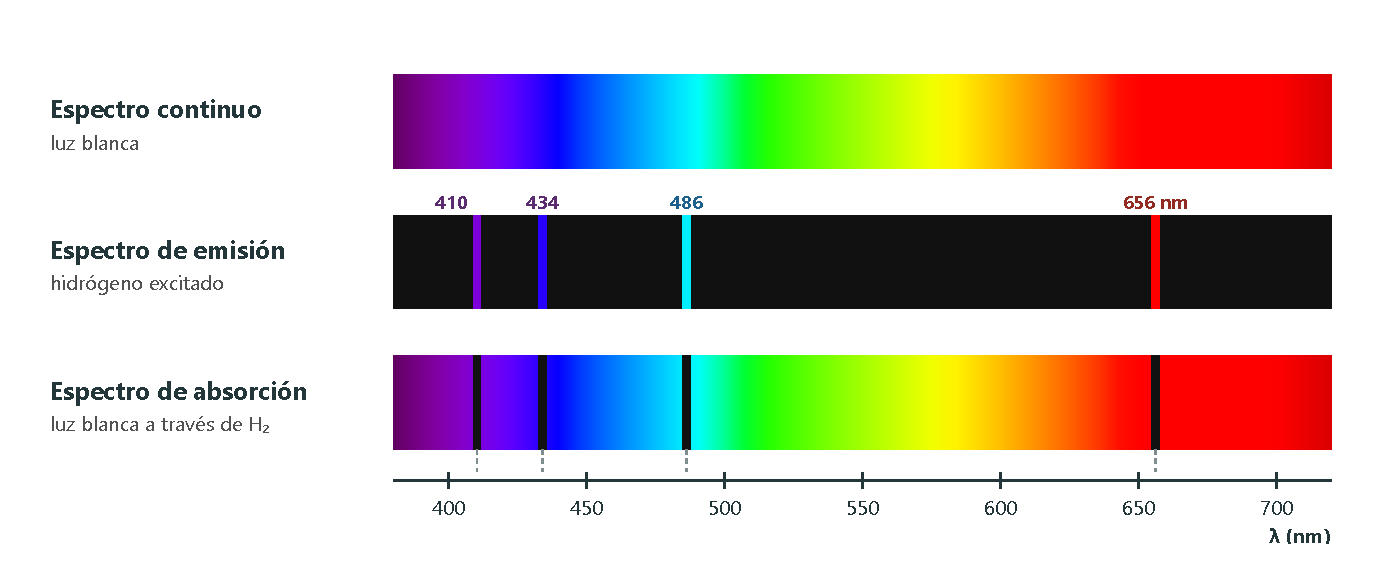
\includegraphics[width=0.8\textwidth]{images/UD3/espectros_atomicos}
    \caption{Espectro continuo y espectros de emisión y de absorción del hidrógeno en la zona visible.}
    \label{fig:ud3-espectros}
\end{figure}

\begin{remark}
    Las frecuencias que absorbe o emite un átomo son \textbf{características} de cada elemento: su espectro es como su
    \textbf{huella dactilar}. Gracias a ello se descubrieron elementos nuevos (el cesio, el rubidio o el helio, que se encontró
    en el espectro del Sol antes que en la Tierra) y hoy se analiza la composición de las estrellas o de una muestra de suelo.
\end{remark}

\paragraph{Series espectrales del hidrógeno.} En 1885, \textbf{J.\,J. Balmer} encontró una fórmula matemática para las rayas
visibles del espectro del hidrógeno, y en 1890 \textbf{J. Rydberg} la generalizó para todas las series que se fueron
descubriendo después:
\[ \frac{1}{\lambda} = R \left( \frac{1}{n_1^2} - \frac{1}{n_2^2} \right) \qquad (n_2 > n_1) \]
donde \(R = \qty{1.097e7}{\per\m}\) es la \textbf{constante de Rydberg}, y \(n_1\) y \(n_2\) son números enteros. Cada valor de
\(n_1\) da una serie de rayas:

\begin{table}[H]
    \centering
    \caption{Series espectrales del hidrógeno}
    \vspace{-5pt}
    \begin{tabular}{@{}lccc@{}}
        \toprule
        \textbf{Serie} & \textbf{Año} & \(\boldsymbol{n_1}\) & \textbf{Zona del espectro} \\
        \midrule
        Lyman & 1906 & 1 & Ultravioleta \\[3pt]
        Balmer & 1885 & 2 & Visible \\[3pt]
        Paschen & 1908 & 3 & Infrarrojo \\[3pt]
        Brackett & 1922 & 4 & Infrarrojo \\[3pt]
        Pfund & 1924 & 5 & Infrarrojo \\
        \bottomrule
    \end{tabular}
    \label{tab:ud3-series}
\end{table}

\begin{example}
    \textbf{Primera raya de la serie de Lyman.} Calcula la longitud de onda de la raya de la serie de Lyman con \(n_2 = 2\). ¿En
    qué zona del espectro está?

    \textbf{Solución.} \(\dfrac{1}{\lambda} = \num{1.097e7} \left( \dfrac{1}{1^2} - \dfrac{1}{2^2} \right) = \num{1.097e7} \cdot
    \num{0.75} = \qty{8.23e6}{\per\m}\), así que \(\lambda = \qty{1.215e-7}{\m} = \qty{121.5}{\nm}\): está en el
    \textbf{ultravioleta}, fuera del visible.
\end{example}

\begin{exercise}
    Calcula la longitud de onda de la raya de la serie de Paschen que corresponde a \(n_2 = 5\).
    \begin{solu}
        \(\dfrac{1}{\lambda} = \num{1.097e7} \left( \dfrac{1}{9} - \dfrac{1}{25} \right) = \qty{7.80e5}{\per\m}\):
        \(\lambda = \textcolor{red}{\qty{1.28e-6}{\m} = \qty{1282}{\nm}}\) (infrarrojo).
    \end{solu}
\end{exercise}

\begin{exercise}
    Una de las rayas de la serie de Balmer tiene una longitud de onda de \qty{486}{\nm}. ¿Cuál es el valor de \(n_2\)?
    \begin{solu}
        \(\dfrac{1}{n_2^2} = \dfrac{1}{4} - \dfrac{1}{R \lambda} = \num{0.25} - \dfrac{1}{\num{1.097e7} \cdot \num{486e-9}} = \num{0.0624}\):
        \(n_2^2 = 16\), \(\textcolor{red}{n_2 = 4}\).
    \end{solu}
\end{exercise}

\subsection{La hipótesis de Planck}

La física clásica, según la cual una radiación de cualquier frecuencia podía intercambiar cualquier cantidad de energía con la
materia, no conseguía explicar los espectros atómicos ni la radiación que emiten los cuerpos calientes.

\begin{definition}[Hipótesis de Planck (1900)]
    \textbf{Max Planck} propuso que los átomos no absorben ni emiten energía de forma continua, sino en \textbf{paquetes}
    indivisibles a los que llamó \textbf{cuantos}. La energía de un cuanto de radiación, o \textbf{fotón}, es:
    \[ E = h \cdot \nu = \frac{h \cdot c}{\lambda} \]
    donde \(\nu\) es la frecuencia de la radiación y \(h = \qty{6.626e-34}{\joule\s}\) es la \textbf{constante de Planck}.
\end{definition}

Planck, que recibió el premio Nobel en 1918, propuso su hipótesis casi como un «truco» matemático para explicar la radiación
de un cuerpo caliente. Pero en 1905 \textbf{A. Einstein} la usó para explicar el \textbf{efecto fotoeléctrico} (la emisión de
electrones de un metal iluminado con luz de frecuencia suficiente), y se vio que era el comienzo de una física nueva: la
\textbf{física cuántica}.

\begin{example}
    \textbf{Energía de un fotón.} El espectro de emisión del helio tiene una raya verde de \qty{501.6}{\nm}. a) ¿Cuál es la energía
    de uno de sus fotones? b) ¿Y la de un mol de fotones?

    \textbf{Solución.} a) Pasamos la longitud de onda a metros y aplicamos la ecuación de Planck:
    \[ E = \frac{h c}{\lambda} = \frac{\qty{6.626e-34}{\joule\s} \cdot \qty{3.00e8}{\m\per\s}}{\qty{501.6e-9}{\m}} = \qty{3.96e-19}{\joule} \]
    b) \(E = \qty{3.96e-19}{\joule}/\text{fotón} \cdot \num{6.022e23}\ \text{fotones}/\unit{\mol} = \qty{2.39e5}{\joule\per\mol} =
    \qty{239}{\kilo\joule\per\mol}\).
\end{example}

\paragraph{La doble naturaleza de la radiación.} Hoy admitimos que la radiación electromagnética, incluida la luz, tiene una
naturaleza \textbf{dual}: se \textbf{propaga} como una \textbf{onda} (por eso se refleja, se refracta o se difracta) e
\textbf{interacciona} con la materia como un conjunto de partículas, los \textbf{fotones}. Los dos aspectos son
complementarios, pero nunca se manifiestan a la vez.

\begin{exercise}
    Calcula la energía de un fotón de las microondas de un horno (\qty{2.45}{\giga\hertz}) y la de un fotón de radiación
    ultravioleta de \qty{250}{\nm}. ¿Por qué la radiación ultravioleta puede dañar el ADN de las células y las microondas no?
    \begin{solu}
        Microondas: \(E = h \nu = \num{6.626e-34} \cdot \num{2.45e9} = \textcolor{red}{\qty{1.62e-24}{\joule}}\). Ultravioleta:
        \(E = \dfrac{h c}{\lambda} = \textcolor{red}{\qty{7.95e-19}{\joule}}\), unas \num{500000} veces más.
        \textcolor{blue}{Un fotón ultravioleta tiene energía suficiente para romper enlaces químicos; los de microondas solo hacen
        vibrar o girar las moléculas (calientan), aunque haya muchísimos.}
    \end{solu}
\end{exercise}

\begin{exercise}
    Explica a un compañero que ha faltado a clase la diferencia entre un espectro continuo, uno de emisión y uno de absorción.
    \begin{solu}
        \textcolor{red}{El continuo contiene todas las frecuencias} (la luz blanca del Sol o de un filamento muy caliente).
        \textcolor{red}{El de emisión son rayas de colores sobre fondo negro}: las frecuencias que emite un elemento excitado.
        \textcolor{red}{El de absorción es un espectro continuo con rayas negras}: las frecuencias que absorbe el elemento al pasar
        la luz a través de él. Las rayas de ambos están en las mismas posiciones.
    \end{solu}
\end{exercise}

%========================================================================================
\section{Hacia el modelo actual del átomo}\label{sec:ud3-actual}
%========================================================================================

A medida que la física cuántica avanzaba y mejoraban los instrumentos de laboratorio, se fue conociendo mejor la estructura del
átomo.

\subsection{El modelo atómico de Bohr}

En 1913, \textbf{Niels Bohr} mejoró el modelo de Rutherford incorporándole la teoría cuántica de Planck.

\begin{definition}[Postulados de Bohr]
    \leavevmode % el título de la definición en su propia línea, la lista debajo
    \begin{enumerate}
        \item Los electrones giran alrededor del núcleo en ciertas \textbf{órbitas circulares estacionarias}, en las que
        \textbf{no emiten energía}, aunque sean cargas aceleradas.
        \item La energía del electrón está \textbf{cuantizada}: solo puede tomar ciertos valores, que dependen del
        \textbf{número cuántico principal}, \(n = 1, 2, 3\dots\) La órbita de menor energía, la más cercana al núcleo, es la del
        \textbf{nivel} \(n = 1\).
        \item El electrón puede \textbf{cambiar de órbita} absorbiendo o emitiendo un \textbf{fotón} cuya energía es igual a la
        diferencia de energía entre los dos niveles (figura~\ref{fig:ud3-foton}):
        \[ |\Delta E| = E_{\text{fotón}} = |E_{\text{final}} - E_{\text{inicial}}| = h \cdot \nu = \frac{h c}{\lambda} \]
    \end{enumerate}
\end{definition}

\begin{figure}[H]
    \centering
    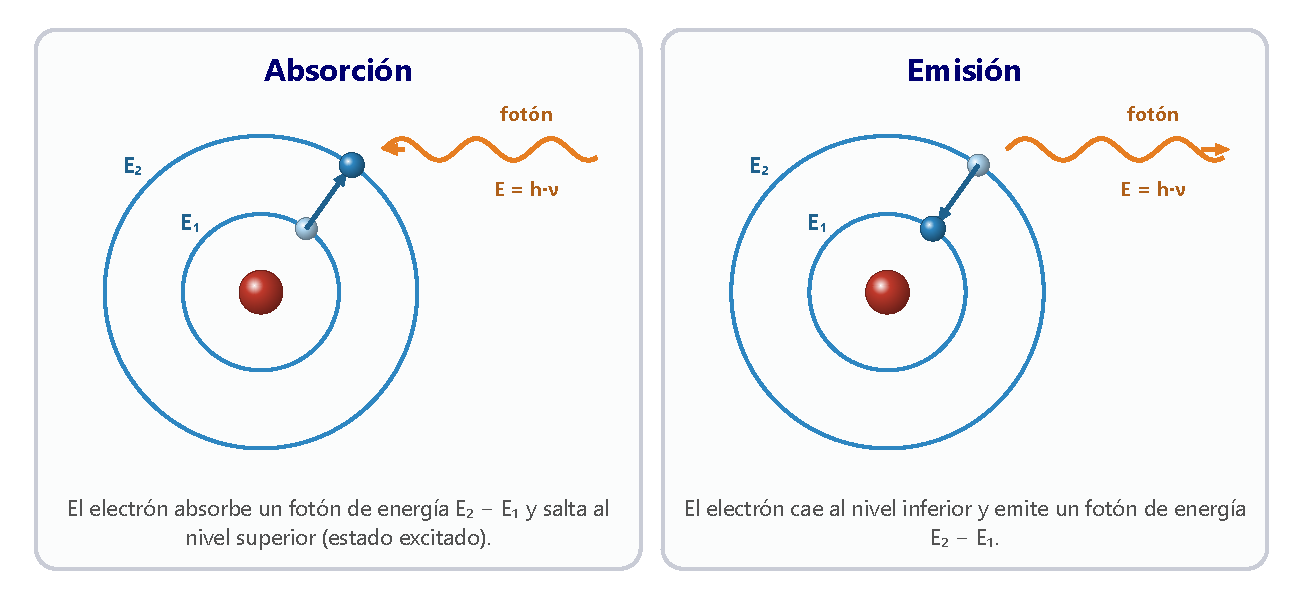
\includegraphics[width=0.72\textwidth]{images/UD3/bohr_foton}
    \caption{Explicación de Bohr para la absorción y la emisión de energía.}
    \label{fig:ud3-foton}
\end{figure}

Para el átomo de hidrógeno, Bohr calculó la energía de cada nivel:
\[ E_n = -\frac{\qty{2.18e-18}{\joule}}{n^2} = -\frac{\qty{13.6}{\electronvolt}}{n^2} \]
La energía es negativa porque se toma como cero la del electrón libre, fuera del átomo (\(n = \infty\)): para separar el
electrón del núcleo hay que darle energía. Con esta expresión se deduce la fórmula de Rydberg, lo que supuso un gran éxito del
modelo.

\paragraph{Interpretación de los espectros atómicos.} El modelo de Bohr explica muy bien los espectros:
\begin{itemize}
    \item Como el electrón no puede tener cualquier energía, solo se absorben o se emiten fotones cuya energía es exactamente la
    diferencia entre dos niveles: por eso los espectros son \textbf{discontinuos}.
    \item Un electrón \textbf{excitado} (en un nivel superior al que le corresponde) es inestable y cae a niveles de menor energía
    emitiendo radiación: es lo que se observa en el espectro de \textbf{emisión}.
    \item La energía de los niveles depende del número atómico, así que cada elemento tiene un espectro \textbf{característico}.
    \item Cada \textbf{serie espectral} corresponde a los saltos que terminan (o empiezan) en un mismo nivel
    (figura~\ref{fig:ud3-series}): la de Lyman, en \(n = 1\); la de Balmer, en \(n = 2\)…
\end{itemize}

\begin{figure}[H]
    \centering
    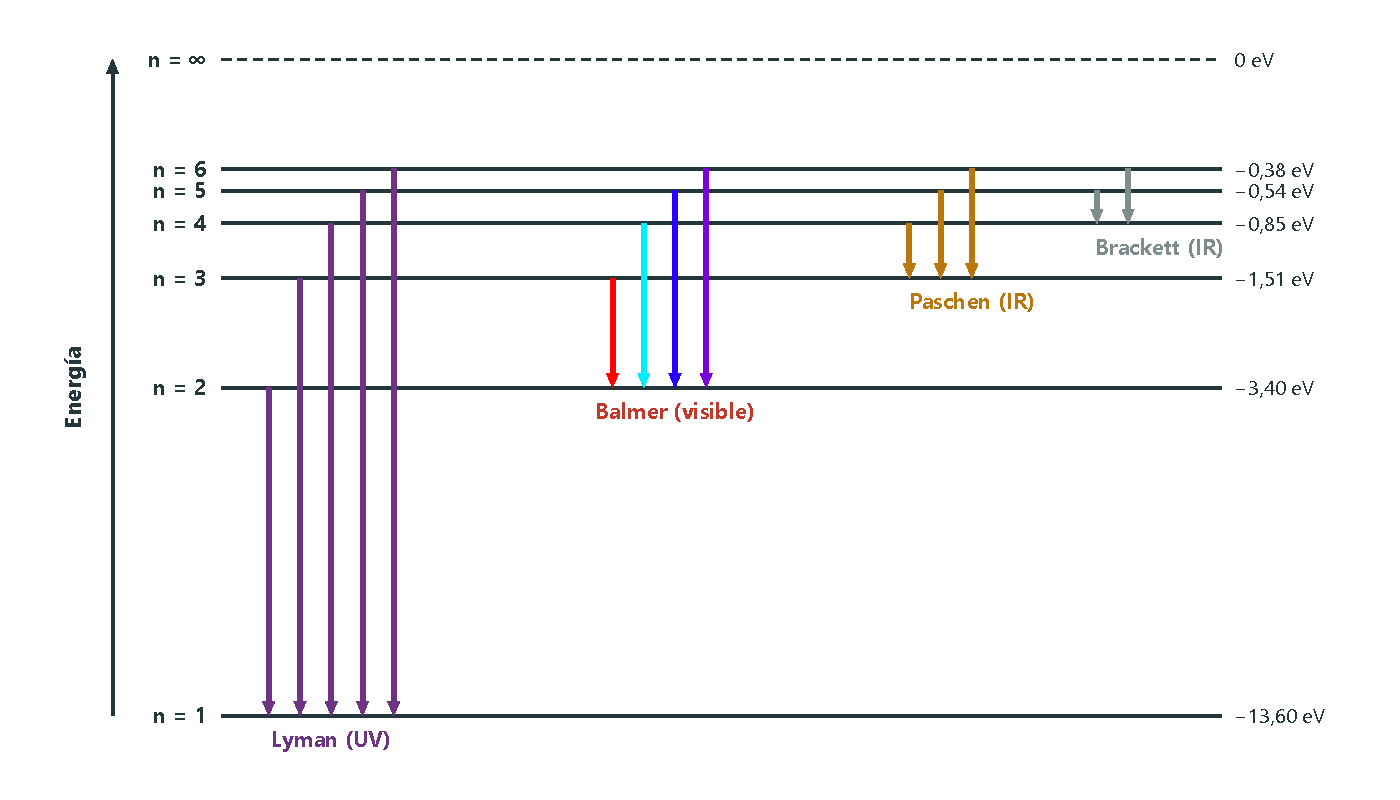
\includegraphics[width=0.8\textwidth]{images/UD3/bohr_series}
    \caption{Niveles de energía del átomo de hidrógeno y series espectrales (escala vertical comprimida para que se distingan los
    niveles altos).}
    \label{fig:ud3-series}
\end{figure}

\begin{example}
    \textbf{Niveles de energía del hidrógeno.} Calcula la energía del electrón del hidrógeno en los cinco primeros niveles.

    \textbf{Solución.} Con \(E_n = -\num{2.18e-18}/n^2\) (en julios) y \(-\num{13.6}/n^2\) (en eV):
    \begin{center}
        \begin{tabular}{@{}cccccc@{}}
            \toprule
            \(\boldsymbol{n}\) & 1 & 2 & 3 & 4 & 5 \\
            \midrule
            \(E_n\) (J) & \num{-2.18e-18} & \num{-5.45e-19} & \num{-2.42e-19} & \num{-1.36e-19} & \num{-8.72e-20} \\[3pt]
            \(E_n\) (eV) & \num{-13.6} & \num{-3.40} & \num{-1.51} & \num{-0.85} & \num{-0.54} \\
            \bottomrule
        \end{tabular}
    \end{center}
    Los niveles están cada vez más próximos entre sí a medida que aumenta \(n\).
\end{example}

\begin{example}
    \textbf{La raya roja del hidrógeno.} Calcula la energía, la frecuencia y la longitud de onda del fotón que emite el electrón
    del hidrógeno al pasar del nivel \(n = 3\) al \(n = 2\).

    \textbf{Solución.} \(\Delta E = E_3 - E_2 = \num{2.18e-18} \left( \dfrac{1}{2^2} - \dfrac{1}{3^2} \right) = \qty{3.03e-19}{\joule}\)
    es la energía del fotón emitido.
    \[ \nu = \frac{E}{h} = \frac{\num{3.03e-19}}{\num{6.626e-34}} = \qty{4.57e14}{\hertz} \qquad
    \lambda = \frac{c}{\nu} = \frac{\num{3.00e8}}{\num{4.57e14}} = \qty{6.56e-7}{\m} = \qty{656}{\nm} \]
    Es la raya roja de la serie de Balmer (figura~\ref{fig:ud3-espectros}).
\end{example}

\begin{exercise}
    a) ¿Qué energía hay que dar al electrón de un átomo de hidrógeno en su estado fundamental (\(n = 1\)) para arrancarlo del
    átomo? Exprésala en julios y en \unit{\kilo\joule\per\mol}. b) ¿Qué longitud de onda máxima debe tener la radiación capaz de
    hacerlo?
    \begin{solu}
        a) Hay que llevarlo de \(E_1\) a \(E_\infty = 0\): \(\textcolor{red}{\qty{2.18e-18}{\joule}}\) por átomo;
        \(\num{2.18e-18} \cdot \num{6.022e23} = \textcolor{red}{\qty{1313}{\kilo\joule\per\mol}}\).
        b) \(\lambda = \dfrac{h c}{E} = \textcolor{red}{\qty{9.12e-8}{\m} = \qty{91.2}{\nm}}\) (ultravioleta).
    \end{solu}
\end{exercise}

\begin{exercise}
    ¿Por qué cada elemento químico tiene un espectro diferente, que sirve para identificarlo?
    \begin{solu}
        \textcolor{red}{Porque la energía de los niveles depende de la carga del núcleo (\(Z\)) y de los demás electrones}: las
        diferencias de energía entre niveles, y por tanto las frecuencias absorbidas o emitidas, son distintas en cada elemento.
    \end{solu}
\end{exercise}

\subsection{Modificaciones al modelo de Bohr}

El modelo de Bohr no podía explicar el espectro de los átomos con más de un electrón, y los espectroscopios, cada vez mejores,
aportaban nuevos datos:
\begin{itemize}
    \item \textbf{A. Sommerfeld} observó en 1915 que algunas rayas eran en realidad dos o más rayas finas muy próximas. Propuso
    que había \textbf{subniveles} de energía y que las órbitas podían ser elípticas.
    \item El \textbf{efecto Zeeman} (1896) es el desdoblamiento de las rayas del espectro en presencia de un campo magnético. Se
    relacionó con distintas \textbf{orientaciones} de las órbitas en el espacio.
    \item \textbf{G. Uhlenbeck} y \textbf{S. Goudsmit} explicaron otro desdoblamiento de las rayas suponiendo que el electrón
    tiene \textbf{propiedades magnéticas} propias, como habían sugerido los experimentos de \textbf{O. Stern} y
    \textbf{W. Gerlach}: el \textbf{espín}.
\end{itemize}
Para describir estos cambios de subnivel, de orientación o de movimiento se introdujeron nuevos números cuánticos: \(l\),
\(m\) y \(s\). En el modelo posterior estos números surgirán de las propias ecuaciones.

\subsection{La contribución de la física cuántica}

En 1924, \textbf{L. de Broglie} propuso que, igual que la luz se comporta a veces como partícula, las partículas (como el
electrón) se comportan a veces como ondas. Poco después apareció otra idea que rompía con la física clásica:

\begin{definition}[Principio de incertidumbre de Heisenberg (1927)]
    Es imposible medir con exactitud, a la vez, la posición y la velocidad de una partícula subatómica como el electrón.
\end{definition}

Esto obliga a abandonar la idea de \textbf{órbita}, una trayectoria definida: no podemos saber a la vez dónde está el electrón y
a qué velocidad se mueve. Solo podemos hablar de la \textbf{probabilidad} de encontrarlo en una zona.

\subsection{El modelo mecanocuántico del átomo}

Había que crear leyes físicas nuevas para describir el mundo subatómico. En 1926, \textbf{E. Schrödinger} formuló una
\textbf{ecuación de onda} para estudiar el movimiento de un electrón ligado a un átomo. Sus soluciones son las
\textbf{funciones de onda}, \(\Psi\), que dependen de cuatro \textbf{números cuánticos}: \(n\), \(l\), \(m\) y \(m_s\). La función
de onda no tiene un significado físico directo, pero \(|\Psi|^2\) indica la \textbf{densidad de probabilidad} de encontrar al
electrón en cada punto (interpretación de Copenhague, de Born, Heisenberg y Bohr, a la que Einstein se opuso con su famosa frase
«Dios no juega a los dados»).

\begin{definition}[Orbital atómico]
    Es la \textbf{región del espacio} alrededor del núcleo en la que la \textbf{probabilidad} de encontrar al electrón con una
    energía determinada es máxima (superior al 90\,\%). Cada orbital queda definido por tres números cuánticos: \(n\), \(l\) y
    \(m\).
\end{definition}

\begin{remark}
    \textbf{Órbita y orbital no son lo mismo.} Una órbita (modelo de Bohr) es una trayectoria circular bien definida; un orbital
    es una «nube» de probabilidad, sin trayectoria, con una forma que depende de \(l\). En 2013 se obtuvo la primera imagen real de
    un átomo de hidrógeno: el electrón no aparece como una bolita, sino como una nube alrededor del núcleo.
\end{remark}

\subsection{Los números cuánticos}

\begin{table}[H]
    \centering
    \caption{Números cuánticos que caracterizan un orbital}
    \vspace{-5pt}
    \begin{tabular}{@{}lL{3.6cm}L{4.4cm}L{3.8cm}@{}}
        \toprule
        & \textbf{Principal, \(\boldsymbol{n}\)} & \textbf{Secundario o azimutal, \(\boldsymbol{l}\)} & \textbf{Magnético, \(\boldsymbol{m}\)} \\
        \midrule
        Valores & \(1, 2, 3\dots\) & \(0, 1, 2\dots, n-1\) & De \(-l\) a \(+l\), incluido el 0 \\[3pt]
        Indica & El \textbf{nivel} de energía & El \textbf{subnivel}: cada nivel tiene \(n\) subniveles & La \textbf{orientación} del orbital en el espacio: cada subnivel tiene \(2l+1\) orbitales \\[3pt]
        Determina & El \textbf{tamaño} del orbital & La \textbf{forma} del orbital & Su orientación \\
        \bottomrule
    \end{tabular}
    \label{tab:ud3-numeros}
\end{table}

Los subniveles se nombran con el valor de \(n\) y una letra según el valor de \(l\):
\[ l = 0 \rightarrow s \qquad l = 1 \rightarrow p \qquad l = 2 \rightarrow d \qquad l = 3 \rightarrow f \]

\begin{table}[H]
    \centering
    \caption{Subniveles y orbitales de los cuatro primeros niveles}
    \vspace{-5pt}
    \begin{tabular}{@{}cccccc@{}}
        \toprule
        \(\boldsymbol{n}\) & \(\boldsymbol{l}\) & \textbf{Subnivel} & \(\boldsymbol{m}\) & \makecell{\textbf{N.º de} \\ \textbf{orbitales}} & \makecell{\textbf{Electrones} \\ \textbf{(máximo)}} \\
        \midrule
        1 & 0 & 1s & 0 & 1 & 2 \\[3pt]
        \cmidrule(lr){1-6}
        2 & 0 & 2s & 0 & 1 & 2 \\
          & 1 & 2p & \(-1, 0, +1\) & 3 & 6 \\[3pt]
        \cmidrule(lr){1-6}
        3 & 0 & 3s & 0 & 1 & 2 \\
          & 1 & 3p & \(-1, 0, +1\) & 3 & 6 \\
          & 2 & 3d & \(-2, -1, 0, +1, +2\) & 5 & 10 \\[3pt]
        \cmidrule(lr){1-6}
        4 & 0 & 4s & 0 & 1 & 2 \\
          & 1 & 4p & \(-1, 0, +1\) & 3 & 6 \\
          & 2 & 4d & \(-2\dots +2\) & 5 & 10 \\
          & 3 & 4f & \(-3\dots +3\) & 7 & 14 \\
        \bottomrule
    \end{tabular}
    \label{tab:ud3-subniveles}
\end{table}

Los orbitales de un mismo subnivel tienen \textbf{la misma energía}. Su forma depende de \(l\) (figura~\ref{fig:ud3-orbitales}):
los \textbf{s} son esféricos; los \textbf{p}, de dos lóbulos orientados según los ejes \(x\), \(y\) o \(z\); y los \textbf{d},
más complejos, casi todos de cuatro lóbulos.

\begin{figure}[H]
    \centering
    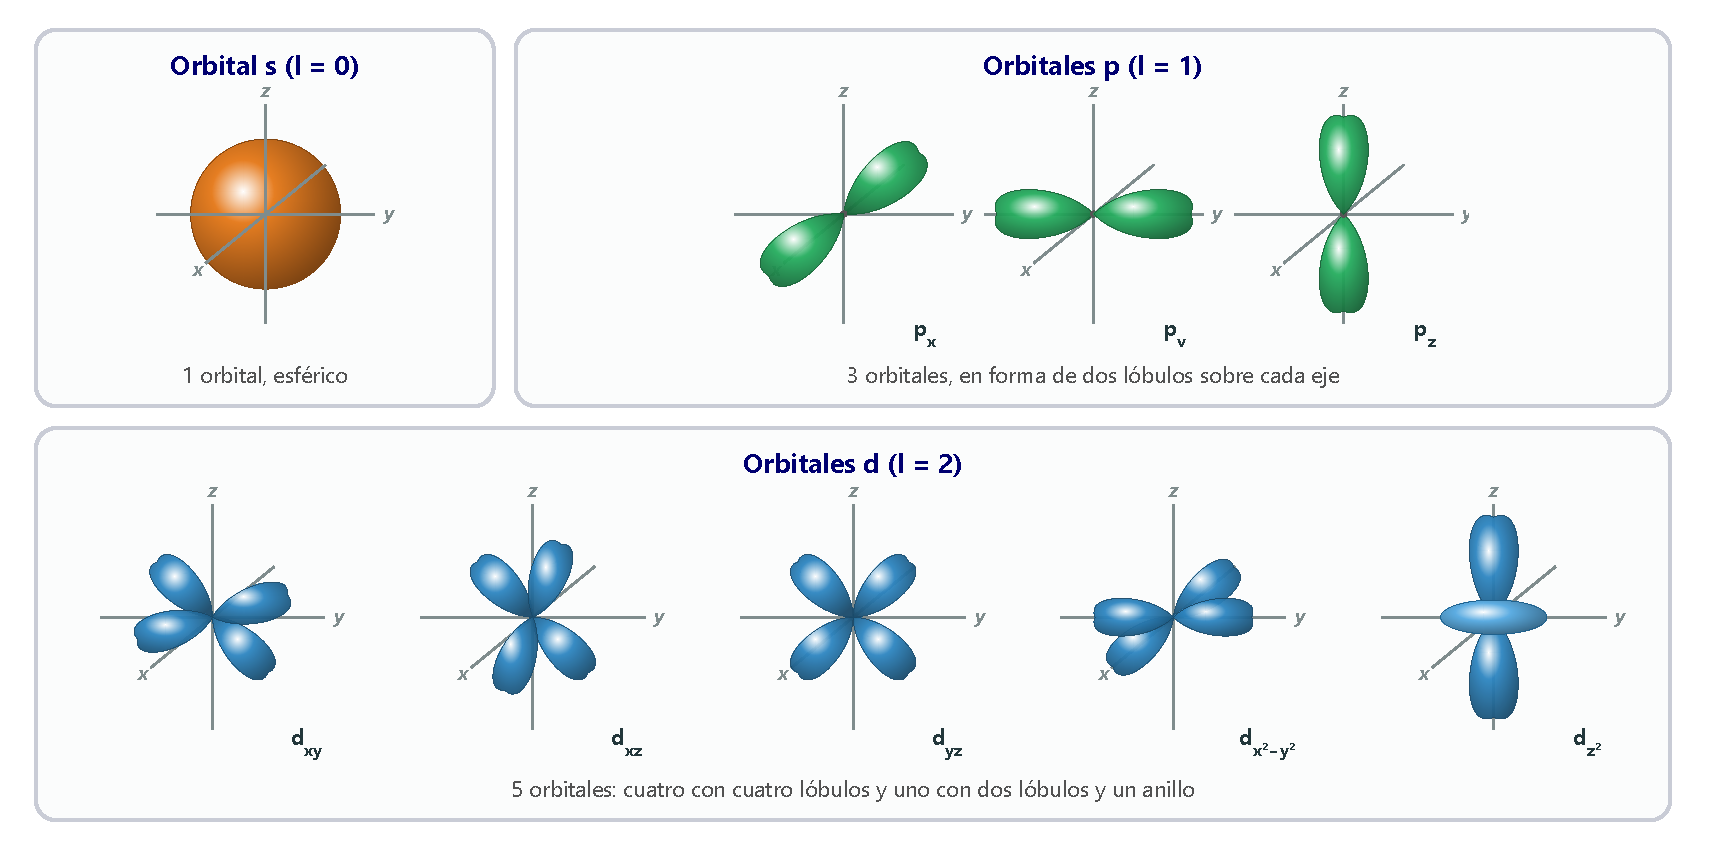
\includegraphics[width=\textwidth]{images/UD3/orbitales}
    \caption{Forma de los orbitales s, p y d.}
    \label{fig:ud3-orbitales}
\end{figure}

\paragraph{El espín del electrón.} Igual que la masa o la carga, el \textbf{espín} es una \textbf{propiedad intrínseca} de las
partículas subatómicas, relacionada con su comportamiento magnético. El \textbf{número cuántico de espín}, \(m_s\), solo puede
valer \(+\frac{1}{2}\) (se representa \(\uparrow\)) o \(-\frac{1}{2}\) (\(\downarrow\)).

El \textbf{estado} de un electrón queda determinado por sus cuatro números cuánticos \((n, l, m, m_s)\): los tres primeros
indican en qué orbital está, y \(m_s\), el sentido de su espín.

\begin{example}
    \textbf{¿Combinaciones posibles?} Indica cuáles de estos conjuntos de números cuánticos \((n, l, m, m_s)\) son posibles y, para
    los que lo sean, en qué orbital está el electrón: a) \((4, 2, -1, +\frac{1}{2})\); b) \((3, 3, 0, -\frac{1}{2})\);
    c) \((2, 1, -2, +\frac{1}{2})\).

    \textbf{Solución.} a) \textbf{Posible}: con \(n = 4\), \(l\) puede valer 0, 1, 2 o 3; con \(l = 2\), \(m\) va de \(-2\) a
    \(+2\), y \(m_s = +\frac{1}{2}\) es válido. Es un electrón de un orbital \textbf{4d}.

    b) \textbf{No es posible}: \(l\) debe ser menor que \(n\) (con \(n = 3\), \(l\) solo puede ser 0, 1 o 2).

    c) \textbf{No es posible}: con \(l = 1\), \(m\) solo puede ser \(-1\), 0 o \(+1\).
\end{example}

\begin{exercise}
    a) Para \(n = 3\), ¿qué valores pueden tomar \(l\) y \(m\)? b) ¿Cuántos orbitales hay en el nivel 3 y cuántos electrones caben
    en él? c) Generaliza: ¿cuántos orbitales y electrones hay en el nivel \(n\)?
    \begin{solu}
        a) \(l = 0\) (\(m = 0\)); \(l = 1\) (\(m = -1, 0, +1\)); \(l = 2\) (\(m = -2\dots+2\)). b) \(1 + 3 + 5 = \textcolor{red}{9}\)
        orbitales y \(\textcolor{red}{18}\) electrones. c) \(\textcolor{red}{n^2}\) orbitales y \(\textcolor{red}{2n^2}\) electrones.
    \end{solu}
\end{exercise}

\begin{exercise}
    Dados los conjuntos de números cuánticos \((4, 2, 1, -\frac{1}{2})\), \((3, 1, -2, +\frac{1}{2})\), \((2, 0, 0, +1)\) y
    \((5, 1, 0, -\frac{1}{2})\): a) ¿cuáles son posibles y por qué? b) ¿En qué orbital está el electrón en los posibles?
    c) ¿Cuál de ellos tiene más energía?
    \begin{solu}
        a) \textcolor{red}{Posibles: el primero y el cuarto.} El segundo no, porque con \(l = 1\), \(m\) no puede ser \(-2\); el
        tercero no, porque \(m_s\) solo vale \(\pm\frac{1}{2}\). b) \textcolor{red}{4d y 5p.} c) Los dos tienen \(n + l = 6\); a
        igualdad, tiene más energía el de mayor \(n\): \textcolor{red}{el 5p} (en el diagrama de Möller va después del 4d).
    \end{solu}
\end{exercise}

\subsection{Configuraciones electrónicas}

La \textbf{configuración electrónica} es la forma en que se distribuyen los electrones de un átomo en sus orbitales. La más
estable es la de menor energía, que se llama \textbf{estado fundamental}. Para escribirla se siguen tres reglas:

\begin{definition}[Reglas para escribir configuraciones electrónicas]
    \leavevmode % el título de la definición en su propia línea, la lista debajo
    \begin{enumerate}
        \item \textbf{Principio de Aufbau} (o de construcción): los electrones van ocupando los subniveles \textbf{de menor a mayor
        energía}. El orden se recuerda con el \textbf{diagrama de Möller} (figura~\ref{fig:ud3-moller}): primero se llenan los
        subniveles con menor \(n + l\), y si dos tienen el mismo, el de menor \(n\).
        \item \textbf{Principio de exclusión de Pauli}: en un átomo no puede haber dos electrones con los cuatro números cuánticos
        iguales. Como \(m_s\) solo tiene dos valores, en un orbital caben como máximo \textbf{dos electrones}, con espines
        opuestos (\(\uparrow\downarrow\)).
        \item \textbf{Regla de máxima multiplicidad de Hund}: los orbitales de un mismo subnivel se llenan de modo que haya el
        \textbf{máximo número de electrones desapareados} (con el mismo espín); solo cuando todos tienen un electrón empiezan a
        aparearse.
    \end{enumerate}
\end{definition}

\begin{figure}[H]
    \centering
    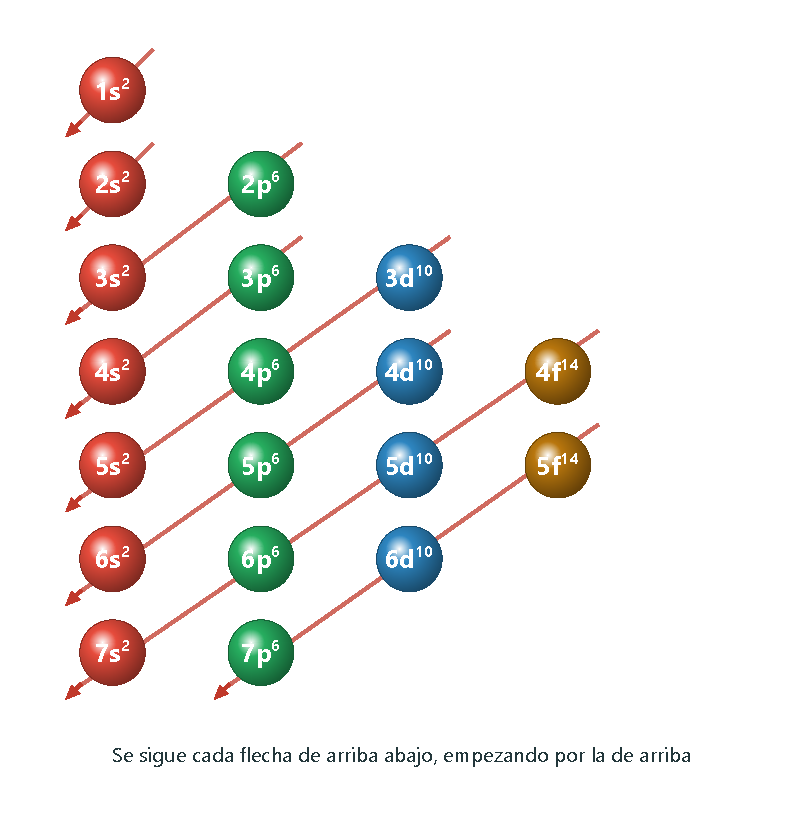
\includegraphics[width=0.45\textwidth]{images/UD3/moller}
    \caption{Diagrama de Möller: orden de llenado de los subniveles. El superíndice es el número máximo de electrones que caben
    en cada subnivel (el doble de sus orbitales).}
    \label{fig:ud3-moller}
\end{figure}

El orden de llenado es: \conf{1s\ 2s\ 2p\ 3s\ 3p\ 4s\ 3d\ 4p\ 5s\ 4d\ 5p\ 6s\ 4f\ 5d\ 6p\ 7s\ 5f\ 6d\ 7p}. Los orbitales se
representan con cajas y los electrones con flechas. Por ejemplo, así se llena un subnivel p según la regla de Hund:
\begin{center}
    \orbcaja{\uparrow}\orbcaja{}\orbcaja{}\quad \orbcaja{\uparrow}\orbcaja{\uparrow}\orbcaja{}\quad \orbcaja{\uparrow}\orbcaja{\uparrow}\orbcaja{\uparrow}\quad
    \orbcaja{\uparrow\downarrow}\orbcaja{\uparrow}\orbcaja{\uparrow}\quad \orbcaja{\uparrow\downarrow}\orbcaja{\uparrow\downarrow}\orbcaja{\uparrow}\quad
    \orbcaja{\uparrow\downarrow}\orbcaja{\uparrow\downarrow}\orbcaja{\uparrow\downarrow}
\end{center}
Un orbital puede estar \textbf{vacío}, \textbf{semilleno} (un electrón desapareado) o \textbf{lleno} (dos electrones apareados).

\paragraph{Átomos e iones.}
\begin{itemize}
    \item Un átomo \textbf{neutro} tiene \(Z\) electrones: el aluminio (\(Z = 13\)) tiene 13: \conf{1s^2\,2s^2\,2p^6\,3s^2\,3p^1}.
    \item Un \textbf{catión} tiene tantos electrones menos como indica su carga: el \ch{Al^3+} tiene \(13 - 3 = 10\) electrones:
    \conf{1s^2\,2s^2\,2p^6}.
    \item Un \textbf{anión} tiene tantos electrones más como indica su carga: el \ch{S^2-} tiene \(16 + 2 = 18\) electrones:
    \conf{1s^2\,2s^2\,2p^6\,3s^2\,3p^6}.
\end{itemize}

\begin{remark}
    \textbf{Los metales de transición pierden primero los electrones 4s.} Aunque el 4s se llena antes que el 3d, una vez ocupado
    el 3d su energía queda por debajo de la del 4s. Por eso, al formar cationes, los metales de transición pierden primero los
    electrones del nivel más externo: \ch{Fe} \conf{[Ar]\,4s^2\,3d^6} \(\rightarrow\) \ch{Fe^2+} \conf{[Ar]\,3d^6}. Hay
    además algunas excepciones a las reglas de llenado, como el cromo (\conf{[Ar]\,4s^1\,3d^5}) y el cobre
    (\conf{[Ar]\,4s^1\,3d^{10}}), que se estabilizan con subniveles d semillenos o llenos.
\end{remark}

\begin{example}
    \textbf{Configuraciones electrónicas.} Escribe la configuración electrónica de: a) N (\(Z = 7\)); b) \ch{Cl^-} (\(Z = 17\));
    c) \ch{Fe^2+} (\(Z = 26\)); d) Br (\(Z = 35\)).

    \textbf{Solución.} Seguimos el orden del diagrama de Möller:

    a) N (7 electrones): \conf{1s^2\,2s^2\,2p^3}.

    b) Cl (17 electrones): \conf{1s^2\,2s^2\,2p^6\,3s^2\,3p^5}.\\
    Al ganar un electrón, \ch{Cl^-} (18 electrones): \conf{1s^2\,2s^2\,2p^6\,3s^2\,3p^6}.

    c) Fe (26 electrones): \conf{1s^2\,2s^2\,2p^6\,3s^2\,3p^6\,4s^2\,3d^6}.\\
    Pierde los dos electrones 4s: \ch{Fe^2+} \conf{1s^2\,2s^2\,2p^6\,3s^2\,3p^6\,3d^6}.

    d) Br (35 electrones): \conf{1s^2\,2s^2\,2p^6\,3s^2\,3p^6\,4s^2\,3d^{10}\,4p^5}.
\end{example}

\begin{example}
    \textbf{¿Estado fundamental o excitado?} ¿Alguna de estas configuraciones corresponde a un átomo en estado excitado?
    a) \conf{1s^2\,2s^2\,2p^6\,3s^2\,3p^4\,4s^1}; b) \conf{1s^2\,2s^2\,2p^6\,3s^2\,3p^6\,4s^2\,3d^3}; c) \conf{1s^2\,2s^2\,2p^4\,3s^1}.

    \textbf{Solución.} a) Tiene 17 electrones; en el estado fundamental el 3p estaría completo (\(3p^5\)) antes de ocupar el 4s:
    es el cloro en un \textbf{estado excitado}. b) Tiene 23 electrones colocados en orden: es el vanadio en su \textbf{estado
    fundamental}. c) Tiene 9 electrones y el 2p no está completo: es el flúor \textbf{excitado} (el fundamental es
    \conf{1s^2\,2s^2\,2p^5}).
\end{example}

\begin{exercise}
    Para el isótopo \ch{^{85}_{37}Rb}, indica: a) el número de protones, neutrones y electrones; b) su configuración electrónica y
    el número de electrones desapareados; c) los números cuánticos de su último electrón; d) el ion más estable que puede formar.
    \begin{solu}
        a) \textcolor{red}{37 p, 48 n y 37 e}. b) \(\textcolor{red}{\conf{1s^2\,2s^2\,2p^6\,3s^2\,3p^6\,4s^2\,3d^{10}\,4p^6\,5s^1}}\);
        \textcolor{red}{un electrón desapareado}. c) \(\textcolor{red}{(5, 0, 0, +\frac{1}{2})}\). d) \textcolor{red}{\ch{Rb^+}}:
        al perder el electrón 5s queda con la configuración del criptón.
    \end{solu}
\end{exercise}

\begin{exercise}
    Ordena de menor a mayor energía los subniveles 3d, 4s, 2p, 5s y 4p, y escribe un conjunto posible de números cuánticos para
    un electrón de cada uno.
    \begin{solu}
        \textcolor{red}{2p \(<\) 4s \(<\) 3d \(<\) 4p \(<\) 5s} (\(n + l\) = 3, 4, 5, 5, 5; a igual \(n + l\), menor \(n\)).
        Por ejemplo: 2p \((2, 1, 0, +\frac{1}{2})\); 4s \((4, 0, 0, -\frac{1}{2})\); 3d \((3, 2, -2, +\frac{1}{2})\);
        4p \((4, 1, 1, +\frac{1}{2})\); 5s \((5, 0, 0, +\frac{1}{2})\).
    \end{solu}
\end{exercise}

\begin{exercise}
    Escribe el diagrama de orbitales (cajas) de la última capa del nitrógeno (\(Z = 7\)) y del oxígeno (\(Z = 8\)), y del subnivel
    3d del hierro (\(Z = 26\)). ¿Cuántos electrones desapareados tiene cada uno?
    \begin{solu}
        N: 2s \orbcaja{\uparrow\downarrow} 2p \orbcaja{\uparrow}\orbcaja{\uparrow}\orbcaja{\uparrow}: \textcolor{red}{3 desapareados}.
        O: 2s \orbcaja{\uparrow\downarrow} 2p \orbcaja{\uparrow\downarrow}\orbcaja{\uparrow}\orbcaja{\uparrow}: \textcolor{red}{2}.
        Fe: 3d \orbcaja{\uparrow\downarrow}\orbcaja{\uparrow}\orbcaja{\uparrow}\orbcaja{\uparrow}\orbcaja{\uparrow}: \textcolor{red}{4}.
    \end{solu}
\end{exercise}

%========================================================================================
\section{La clasificación periódica de los elementos}\label{sec:ud3-tabla}
%========================================================================================

El oro, la plata o el cobre se conocen desde la Antigüedad, pero fue en el siglo XVIII cuando empezaron a aislarse elementos en
el laboratorio. En el siglo XIX, la electrólisis y la espectroscopía permitieron descubrir muchos más: en 1830 se conocían 55. El
estudio de la radiactividad, en el siglo XX, elevó la cifra hasta los \textbf{118} elementos actuales, de los cuales una veintena
se han sintetizado en aceleradores de partículas o reactores nucleares y no se han encontrado en la naturaleza.

\subsection{Clasificando los elementos a lo largo de la historia}

Pronto se vio que algunos elementos tenían propiedades químicas y físicas parecidas. ¿Qué criterio permitiría clasificarlos?
\begin{itemize}
    \item \textbf{J.\,W. Döbereiner} (1780-1849) formó grupos de tres elementos parecidos, ordenados por masa atómica, las
    \textbf{tríadas}: cloro, bromo y yodo; azufre, selenio y teluro.
    \item \textbf{A. de Chancourtois} (1862) colocó los elementos en una espiral sobre un cilindro y descubrió la
    \textbf{periodicidad}: las propiedades se repetían a intervalos regulares.
    \item \textbf{J. Newlands} ordenó los elementos por su masa en \textbf{octavas}: el octavo se parecía al primero, como las
    notas musicales.
    \item \textbf{D. Mendeléiev} (1869) y, poco después, \textbf{L. Meyer} ordenaron los elementos por su masa atómica en una
    \textbf{tabla}, de forma que en la misma columna quedaran los elementos de propiedades semejantes. Mendeléiev dejó
    \textbf{huecos} para elementos aún desconocidos, cuyas propiedades predijo con acierto (como el galio o el germanio), y
    cambió de orden algunos elementos para que quedaran en la familia que les correspondía por sus propiedades.
    \item \textbf{H. Moseley} (1913) midió la carga nuclear de los átomos y demostró que el número atómico \(Z\) es característico
    de cada elemento. Ordenándolos por \(Z\) y no por su masa, cada elemento encajaba en su familia de forma natural.
\end{itemize}

\begin{remark}
    \textbf{Mujeres y elementos.} Marie Skłodowska-Curie descubrió el polonio y el radio, y el curio lleva su nombre y el de su
    marido; Lise Meitner encontró un isótopo del protactinio, y el meitnerio se llama así en su honor; Ida Noddack descubrió el
    renio, y Marguerite Perey, el francio.
\end{remark}

\subsection{La tabla periódica actual}

A partir de la propuesta de Mendeléiev y de las aportaciones posteriores se llegó a la tabla actual
(figura~\ref{fig:ud3-tabla}). Los elementos están ordenados por su número atómico en \textbf{7 filas o periodos} y
\textbf{18 columnas o grupos}, numerados del 1 al 18. Los elementos de un mismo grupo tienen propiedades semejantes y forman una
\textbf{familia}. Los periodos 6 y 7 tienen 14 elementos más cada uno, que se colocan aparte, debajo de la tabla, para que no
quede demasiado ancha.

\begin{figure}[H]
    \centering
    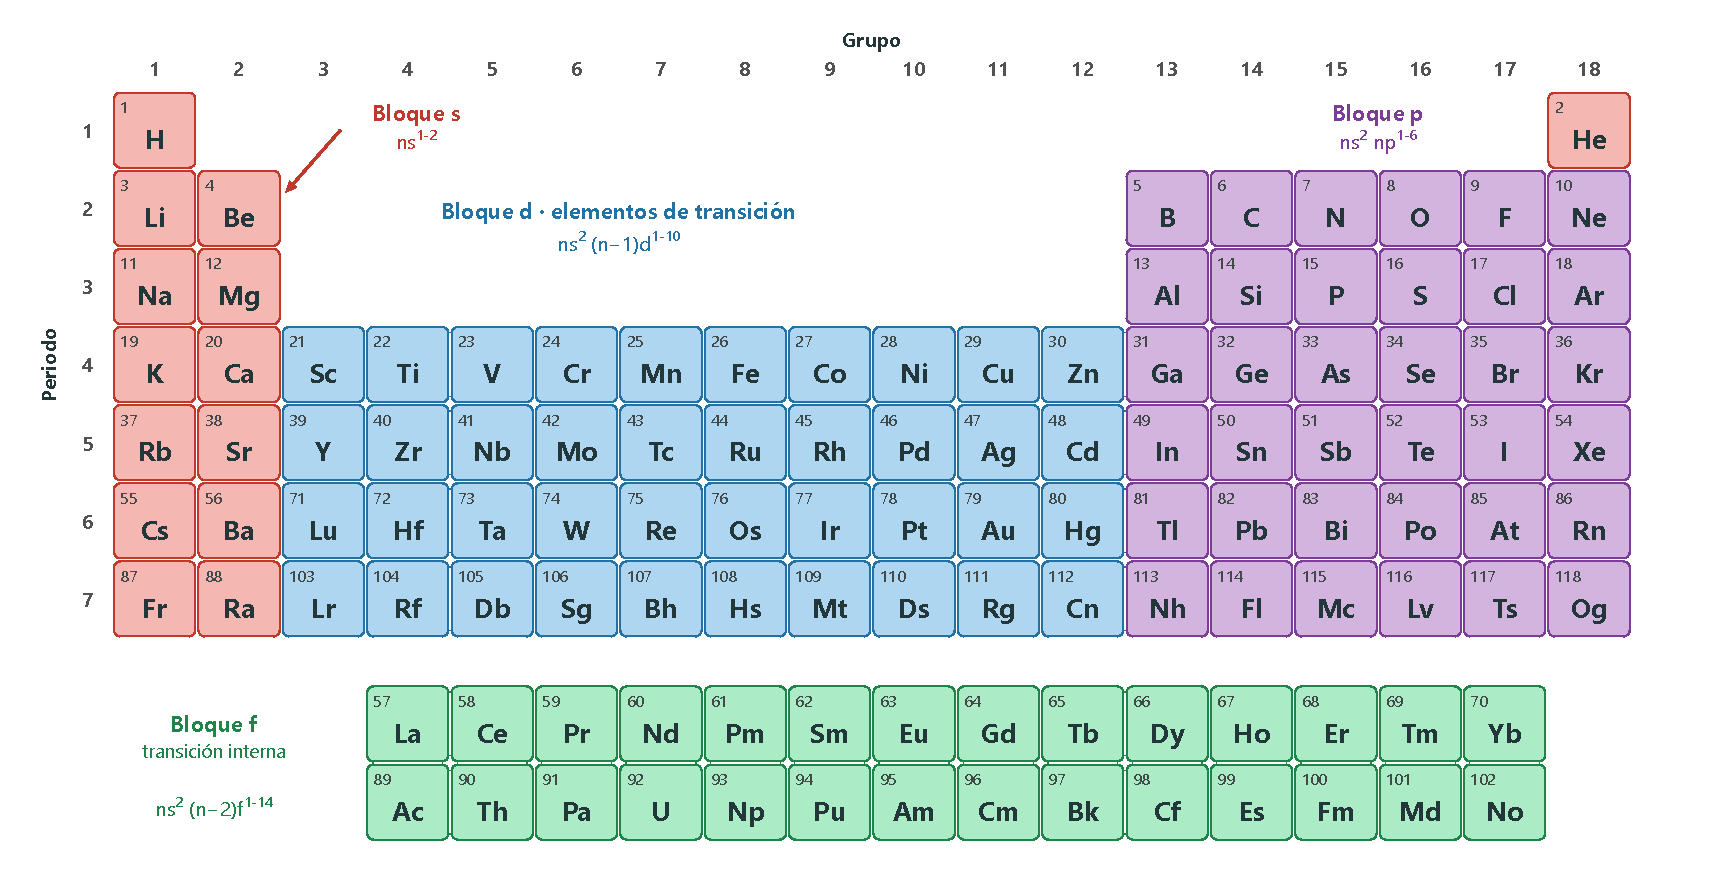
\includegraphics[width=\textwidth]{images/UD3/tabla_bloques}
    \caption{Tabla periódica actual, con los bloques s, p, d y f.}
    \label{fig:ud3-tabla}
\end{figure}

\subsection{Tabla periódica y configuración electrónica}

¿Por qué el berilio (\(Z = 4\)) y el bario (\(Z = 56\)) se parecen? ¿Por qué las propiedades se repiten a intervalos regulares?
Bohr fue el primero en relacionar la configuración electrónica con la posición en la tabla. Fíjate en los elementos del grupo 1:
\begin{center}
    Li \conf{1s^2\,2s^1} \qquad Na \conf{1s^2\,2s^2\,2p^6\,3s^1} \qquad K \conf{[Ne]\,3s^2\,3p^6\,4s^1} \qquad Rb \conf{[Ar]\,4s^2\,3d^{10}\,4p^6\,5s^1}
\end{center}
Todos tienen \textbf{un solo electrón} en el orbital s del último nivel: su configuración termina en \conf{ns^1}.

\begin{definition}[Capa de valencia]
    Es el último nivel (el más externo) en el que hay electrones. Sus electrones se llaman \textbf{electrones de valencia}, y son
    los que determinan las propiedades químicas del elemento.
\end{definition}

\begin{remark}
    Para abreviar, la configuración se escribe a menudo a partir de la del \textbf{gas noble anterior}, entre corchetes:
    Fe \conf{1s^2\,2s^2\,2p^6\,3s^2\,3p^6\,4s^2\,3d^6} = \conf{[Ar]\,4s^2\,3d^6}.
\end{remark}

\begin{itemize}
    \item Los elementos de un \textbf{grupo} tienen el mismo número de electrones en la última capa, en orbitales del mismo tipo.
    \item El valor más alto de \(n\) de la configuración indica el \textbf{periodo}.
    \item Según el último subnivel que se llena, la tabla se divide en \textbf{bloques} (figura~\ref{fig:ud3-tabla}):
    \begin{itemize}
        \item \textbf{Bloque s} (grupos 1 y 2): terminan en \conf{ns^1} o \conf{ns^2}.
        \item \textbf{Bloque p} (grupos 13 a 18): terminan en \conf{ns^2\,np^1} a \conf{ns^2\,np^6}. El \textbf{helio},
        \conf{1s^2}, se coloca en el grupo 18 porque, como los demás \textbf{gases nobles}, tiene su última capa completa.
        \item \textbf{Bloque d} (grupos 3 a 12), los \textbf{metales de transición}: sus últimos electrones van a orbitales d del
        \textbf{penúltimo} nivel, \(n - 1\). El hierro, por ejemplo, termina en \conf{4s^2\,3d^6}.
        \item \textbf{Bloque f}, los elementos de \textbf{transición interna} (lantánidos y actínidos), en dos filas de 14
        elementos de los periodos 6 y 7: sus últimos electrones van a orbitales f del \textbf{antepenúltimo} nivel, \(n - 2\).
        El uranio, por ejemplo, es \conf{[Rn]\,7s^2\,5f^4} (en realidad, \conf{[Rn]\,7s^2\,5f^3\,6d^1}).
    \end{itemize}
\end{itemize}

\begin{remark}
    La configuración electrónica de un elemento determina sus propiedades físicas y químicas. Por eso los elementos de un mismo
    grupo, con la misma configuración de la capa de valencia, se parecen tanto.
\end{remark}

\begin{example}
    \textbf{Elementos del mismo grupo.} Escribe la configuración de tres elementos del grupo 2 y de tres del grupo 17. ¿Qué
    tienen en común los de cada grupo?

    \textbf{Solución.} Grupo 2: Be \conf{1s^2\,2s^2}; Mg \conf{1s^2\,2s^2\,2p^6\,3s^2}; Ca \conf{1s^2\,2s^2\,2p^6\,3s^2\,3p^6\,4s^2}.
    Grupo 17: F \conf{1s^2\,2s^2\,2p^5}; Cl \conf{1s^2\,2s^2\,2p^6\,3s^2\,3p^5}; Br \conf{[Ar]\,4s^2\,3d^{10}\,4p^5}.

    Los del grupo 2 tienen una capa de valencia \conf{ns^2}, con 2 electrones de valencia; los del grupo 17, \conf{ns^2\,np^5},
    con 7 electrones de valencia.
\end{example}

\begin{example}
    \textbf{Posición en la tabla.} Escribe la configuración electrónica de O (\(Z = 8\)), Na (\(Z = 11\)), Si (\(Z = 14\)) y
    Ca (\(Z = 20\)) y, a partir de ella, indica su grupo y su periodo.

    \textbf{Solución.} O \conf{1s^2\,2s^2\,2p^4}: termina en \conf{ns^2\,np^4} con \(n = 2\): grupo 16, periodo 2.
    Na \conf{1s^2\,2s^2\,2p^6\,3s^1}: \conf{ns^1}, grupo 1, periodo 3. Si \conf{1s^2\,2s^2\,2p^6\,3s^2\,3p^2}: \conf{ns^2\,np^2},
    grupo 14, periodo 3. Ca \conf{[Ar]\,4s^2}: \conf{ns^2}, grupo 2, periodo 4.
\end{example}

\begin{exercise}
    Un elemento está en el periodo 4 y en el grupo 15. a) Escribe su configuración electrónica. b) ¿Cuál es su número atómico y de
    qué elemento se trata? c) ¿Cuántos electrones desapareados tiene?
    \begin{solu}
        a) Termina en \conf{4s^2\,4p^3}: \(\textcolor{red}{\conf{1s^2\,2s^2\,2p^6\,3s^2\,3p^6\,4s^2\,3d^{10}\,4p^3}}\).
        b) \(\textcolor{red}{Z = 33}\): \textcolor{red}{arsénico}. c) \textcolor{red}{3} (uno en cada orbital 4p).
    \end{solu}
\end{exercise}

%========================================================================================
\subsection{Propiedades periódicas}
%========================================================================================

Hay propiedades que dependen de la configuración electrónica y que, por tanto, \textbf{varían de forma periódica} a lo largo de
la tabla. Para entenderlas hay que pensar en las fuerzas que actúan sobre los electrones de la capa de valencia. Las cargas
eléctricas se atraen si son de signo contrario y se repelen si son del mismo signo, con una fuerza que, según la
\textbf{ley de Coulomb}, es
\[ F = K \frac{q \cdot q'}{r^2} \]
mayor cuanto mayores son las cargas y menor la distancia que las separa. Así:
\begin{itemize}
    \item Cada electrón es \textbf{atraído} por el núcleo, cuya carga es \(Z\) veces la carga elemental: la atracción aumenta con
    \(Z\) y disminuye con la distancia al núcleo.
    \item A la vez, cada electrón es \textbf{repelido} por los demás electrones: la atracción del núcleo sobre los electrones
    externos queda \textbf{apantallada} por los electrones de las capas internas. La carga que «sienten» de verdad los
    electrones de valencia es la \textbf{carga nuclear efectiva}.
\end{itemize}

\paragraph{Radio atómico.}

\begin{definition}[Radio atómico]
    Es la distancia del núcleo al electrón más externo. Como el átomo no tiene un borde definido, se calcula como la mitad de la
    distancia entre los núcleos de dos átomos iguales unidos.
\end{definition}

\begin{itemize}
    \item En un \textbf{grupo}, el radio \textbf{aumenta hacia abajo}: cada elemento tiene una capa electrónica más que el
    anterior. Por ejemplo, Li \qty{152}{\pico\metre}, Na \qty{186}{\pico\metre}, K \qty{227}{\pico\metre}, Rb
    \qty{248}{\pico\metre}, Cs \qty{265}{\pico\metre}.
    \item En un \textbf{periodo}, el radio \textbf{disminuye hacia la derecha}: los electrones se colocan en la misma capa, pero
    la carga nuclear efectiva aumenta y los atrae con más fuerza. Por ejemplo, en el periodo 2: Li 152, Be 112, B 88, C 77,
    N 75, O 73, F \qty{72}{\pico\metre}.
\end{itemize}

\begin{figure}[H]
    \centering
    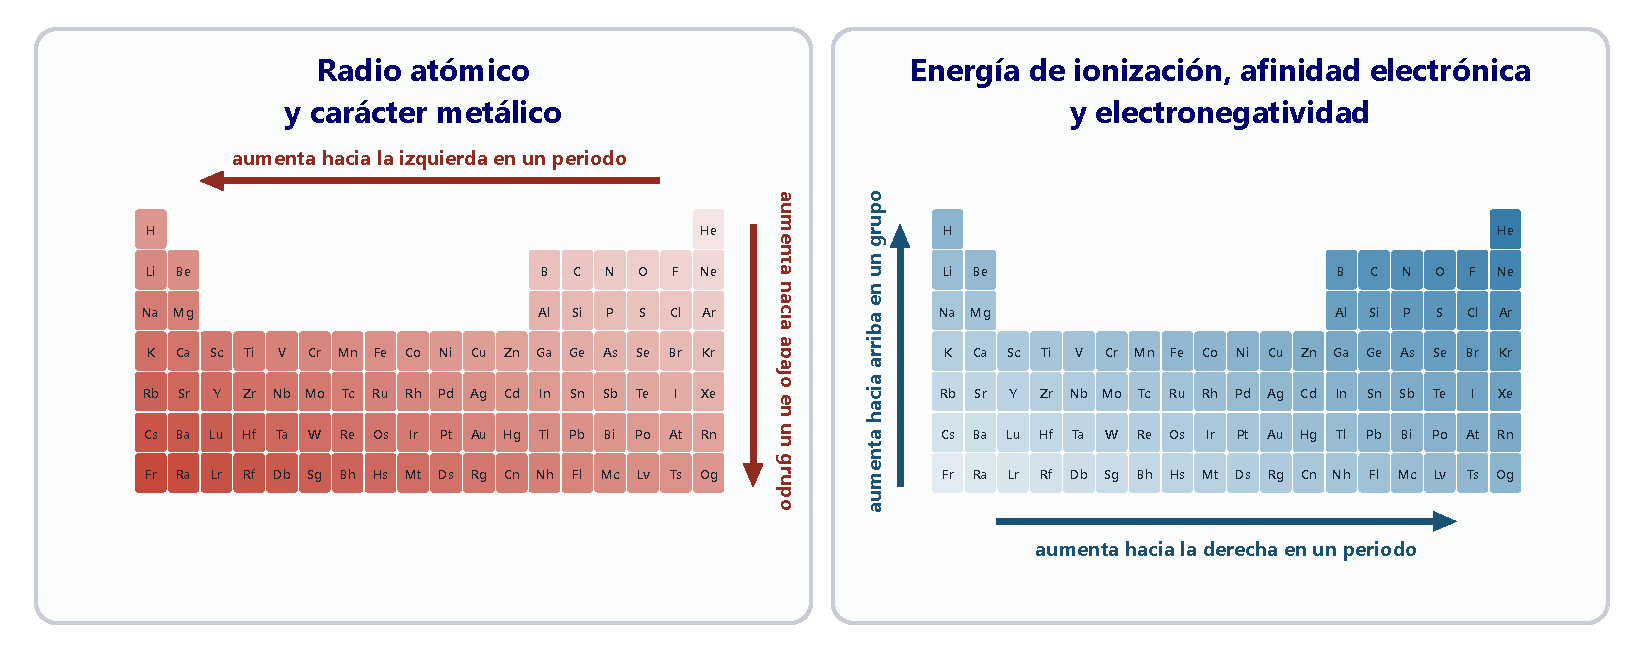
\includegraphics[width=\textwidth]{images/UD3/tendencias}
    \caption{Variación de las propiedades periódicas (cuanto más oscuro, mayor es el valor).}
    \label{fig:ud3-tendencias}
\end{figure}

\paragraph{Radio iónico.} El tamaño de un ion es distinto del de su átomo neutro (figura~\ref{fig:ud3-radios}):
\begin{itemize}
    \item Un \textbf{catión} es \textbf{más pequeño} que su átomo: suele perder la capa más externa y los electrones restantes son
    atraídos con más fuerza por el mismo número de protones.
    \item Un \textbf{anión} es \textbf{más grande} que su átomo: el electrón ganado aumenta la repulsión entre electrones y el
    apantallamiento, y la nube electrónica se expande.
\end{itemize}

\begin{figure}[H]
    \centering
    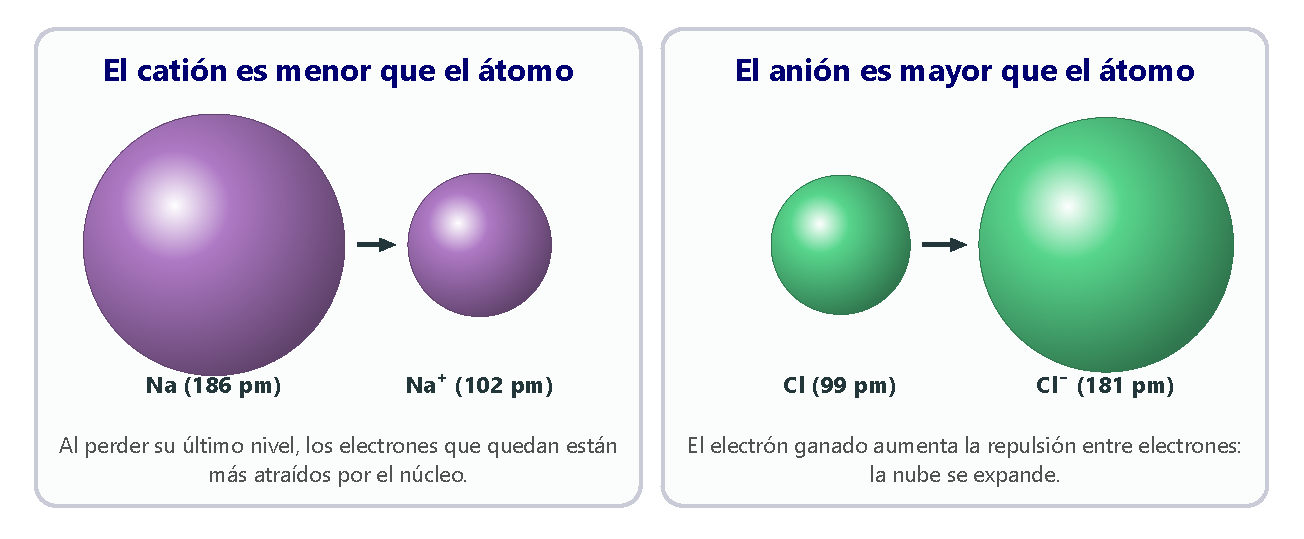
\includegraphics[width=0.75\textwidth]{images/UD3/radios_ionicos}
    \caption{Radios de los átomos de sodio y cloro y de sus iones.}
    \label{fig:ud3-radios}
\end{figure}

\begin{example}
    \textbf{Ordenar por radio atómico.} Ordena de menor a mayor radio atómico: a) Be, Mg, Ca, Sr; b) K, Ca, Ga, Br.

    \textbf{Solución.} a) Son del grupo 2: el radio aumenta al bajar en el grupo, porque hay más capas:
    \(\mathrm{Be} < \mathrm{Mg} < \mathrm{Ca} < \mathrm{Sr}\).

    b) Son del periodo 4: el radio disminuye hacia la derecha, porque aumenta la carga nuclear efectiva:
    \(\mathrm{Br} < \mathrm{Ga} < \mathrm{Ca} < \mathrm{K}\).
\end{example}

\paragraph{Energía de ionización.}

\begin{definition}[Energía de ionización]
    Es la energía necesaria para \textbf{arrancar el electrón más externo} de un átomo en estado gaseoso y fundamental,
    convirtiéndolo en un ion positivo:
    \[ \ch{X(g)} + \text{energía de ionización} \rightarrow \ch{X^+(g) + e^-} \]
    Se suele dar en \unit{\kilo\joule\per\mol}: la energía necesaria para ionizar un mol de átomos. También se usa el
    \textbf{electronvolt} por átomo: \(\qty{1}{\electronvolt} = \qty{1.602e-19}{\joule}\), y
    \(\qty{1}{\electronvolt}/\text{átomo} =\qty{96.49}{\kilo\joule\per\mol}\).
\end{definition}

Cuanto más alejado del núcleo esté el electrón, más débilmente unido está y más fácil es arrancarlo. Por eso la energía de
ionización varía al revés que el radio atómico:
\begin{itemize}
    \item En un \textbf{grupo}, \textbf{aumenta hacia arriba}: Cs 376, Rb 403, K 419, Na 496, Li \qty{520}{\kilo\joule\per\mol}.
    \item En un \textbf{periodo}, \textbf{aumenta hacia la derecha}, y es máxima en los gases nobles (figura~\ref{fig:ud3-ei}).
\end{itemize}

\begin{figure}[H]
    \centering
    \begin{tikzpicture}
        \begin{axis}[grafica, width=0.85\linewidth, height=5.5cm, xmin=0, xmax=21, ymin=0, ymax=2600,
            xtick={1,...,20}, xticklabels={H,He,Li,Be,B,C,N,O,F,Ne,Na,Mg,Al,Si,P,S,Cl,Ar,K,Ca},
            xlabel={Elemento}, ylabel={\(E_i\) (kJ/mol)}, x tick label style={font=\scriptsize},
            y tick label style={/pgf/number format/1000 sep={}}]
            \addplot[ocre, thick, mark=*, mark size=1.6pt] coordinates {(1,1312) (2,2372) (3,520) (4,900) (5,801) (6,1086) (7,1402)
                (8,1314) (9,1681) (10,2081) (11,496) (12,738) (13,578) (14,787) (15,1012) (16,1000) (17,1251) (18,1521) (19,419) (20,590)};
            \node[font=\scriptsize, anchor=south] at (axis cs:2,2372) {gases nobles};
            \node[font=\scriptsize, anchor=north] at (axis cs:11,450) {alcalinos};
        \end{axis}
    \end{tikzpicture}
    \caption{Primera energía de ionización de los 20 primeros elementos: máximos en los gases nobles y mínimos en los alcalinos.}
    \label{fig:ud3-ei}
\end{figure}

\begin{remark}
    \textbf{Energías de ionización sucesivas.} La \textbf{segunda energía de ionización} es la necesaria para arrancar un segundo
    electrón al ion \ch{X^+}, y así sucesivamente. Cada una es mayor que la anterior, porque se arranca un electrón a un ion
    cada vez más positivo, pero el aumento no es uniforme: se dispara cuando el electrón sale de una capa completa. Para el
    magnesio, \conf{[Ne]\,3s^2}:
    \[ E_{i,1} = \qty{738}{\kilo\joule\per\mol} \qquad E_{i,2} = \qty{1451}{\kilo\joule\per\mol} \qquad E_{i,3} = \qty{7733}{\kilo\joule\per\mol} \]
    El tercer electrón hay que sacarlo del nivel 2, completo y mucho más cercano al núcleo. Por eso el magnesio forma iones
    \ch{Mg^2+} y no \ch{Mg^3+}.
\end{remark}

\begin{example}
    \textbf{Ordenar por energía de ionización.} Ordena de menor a mayor primera energía de ionización: a) Li, Na, K, Cs;
    b) Na, Si, P, Cl.

    \textbf{Solución.} a) Son del grupo 1: la energía de ionización aumenta al subir en el grupo:
    \(\mathrm{Cs} < \mathrm{K} < \mathrm{Na} < \mathrm{Li}\).

    b) Son del periodo 3: aumenta hacia la derecha: \(\mathrm{Na} < \mathrm{Si} < \mathrm{P} < \mathrm{Cl}\) (los valores reales
    son 496, 787, 1012 y \qty{1251}{\kilo\joule\per\mol}).
\end{example}

\paragraph{Afinidad electrónica.} Es la energía que se intercambia cuando un átomo en estado gaseoso y fundamental
\textbf{capta un electrón} y se convierte en un ion negativo: \(\ch{X(g) + e^-} \rightarrow \ch{X^-(g)}\). Normalmente se
desprende energía (por eso suele tener signo negativo), y cuanta más se desprende, mayor es la tendencia del átomo a captar
electrones. La afinidad electrónica es mayor (en valor absoluto) \textbf{hacia arriba en un grupo} y \textbf{hacia la derecha en
un periodo}, sin contar los gases nobles: el cloro (\qty{-349}{\kilo\joule\per\mol}) y el flúor
(\qty{-328}{\kilo\joule\per\mol}) son los que más energía desprenden.

\paragraph{Electronegatividad.}

\begin{definition}[Electronegatividad]
    Es una medida de la \textbf{tendencia} de un átomo a \textbf{atraer} hacia sí los electrones del enlace que comparte con otro
    átomo.
\end{definition}

Los valores de electronegatividad se asignan \textbf{comparando} unos elementos con otros. En la escala de \textbf{Pauling}, el
más electronegativo, el flúor, tiene un 4,0. La electronegatividad \textbf{aumenta hacia arriba en un grupo} y \textbf{hacia la
derecha en un periodo} (los gases nobles, que casi no forman enlaces, no tienen valor asignado).

\begin{table}[H]
    \centering
    \caption{Electronegatividad de Pauling de los elementos representativos}
    \vspace{-5pt}
    \begin{tabular}{@{}lccccccc@{}}
        \toprule
        \textbf{Periodo} & \textbf{G. 1} & \textbf{G. 2} & \textbf{G. 13} & \textbf{G. 14} & \textbf{G. 15} & \textbf{G. 16} & \textbf{G. 17} \\
        \midrule
        1 & H 2,2 & & & & & & \\[3pt]
        2 & Li 1,0 & Be 1,6 & B 2,0 & C 2,6 & N 3,0 & O 3,4 & F 4,0 \\[3pt]
        3 & Na 0,9 & Mg 1,3 & Al 1,6 & Si 1,9 & P 2,2 & S 2,6 & Cl 3,2 \\[3pt]
        4 & K 0,8 & Ca 1,0 & Ga 1,8 & Ge 2,0 & As 2,2 & Se 2,6 & Br 3,0 \\[3pt]
        5 & Rb 0,8 & Sr 1,0 & In 1,8 & Sn 2,0 & Sb 2,1 & Te 2,1 & I 2,7 \\[3pt]
        6 & Cs 0,8 & Ba 0,9 & Tl 1,6 & Pb 2,3 & Bi 2,0 & Po 2,0 & At 2,2 \\
        \bottomrule
    \end{tabular}
    \label{tab:ud3-en}
\end{table}

\paragraph{Carácter metálico.} Los \textbf{metales} tienden a perder electrones y formar cationes: tienen energía de ionización
y electronegatividad bajas. Cuanto menor es la electronegatividad de un elemento, mayor es su \textbf{carácter metálico}, que
aumenta \textbf{hacia abajo y hacia la izquierda} de la tabla. Los \textbf{no metales}, a la derecha y arriba, tienden a captar
electrones y formar aniones.

\begin{example}
    \textbf{Ordenar por electronegatividad.} Ordena de menor a mayor electronegatividad: Rb, Ti, As, O y F.

    \textbf{Solución.} La electronegatividad aumenta hacia arriba y hacia la derecha. El Rb (grupo 1, periodo 5) es el que está
    más abajo y a la izquierda, y el F, el que está más arriba y a la derecha. El Ti y el As están en el periodo 4, el Ti más a
    la izquierda; el O está en el periodo 2:
    \(\mathrm{Rb} < \mathrm{Ti} < \mathrm{As} < \mathrm{O} < \mathrm{F}\) (0,8; 1,5; 2,2; 3,4 y 4,0).
\end{example}

\begin{exercise}
    Para la pareja de elementos K y Br, razona: a) cuál tiene mayor radio; b) cuál tiene mayor energía de ionización; c) cuál es
    más electronegativo.
    \begin{solu}
        Los dos están en el periodo 4; el K en el grupo 1 y el Br en el 17. a) \textcolor{red}{El K}: el radio disminuye hacia la
        derecha. b) \textcolor{red}{El Br}: la energía de ionización aumenta hacia la derecha. c) \textcolor{red}{El Br}.
    \end{solu}
\end{exercise}

\begin{exercise}
    Para los elementos A (\(Z = 17\)) y B (\(Z = 20\)): a) escribe sus configuraciones electrónicas; b) indica el ion más estable de
    cada uno; c) ¿cuál de los dos iones tiene mayor radio?
    \begin{solu}
        a) A: \conf{1s^2\,2s^2\,2p^6\,3s^2\,3p^5} (cloro); B: \conf{1s^2\,2s^2\,2p^6\,3s^2\,3p^6\,4s^2} (calcio).
        b) \textcolor{red}{\ch{A^-} (\ch{Cl^-}) y \ch{B^2+} (\ch{Ca^2+})}: ambos adquieren la configuración del argón.
        c) Los dos iones tienen 18 electrones, pero el \ch{Cl^-} solo 17 protones frente a los 20 del \ch{Ca^2+}, que atrae más
        a sus electrones: \textcolor{red}{el \ch{Cl^-} es mayor}.
    \end{solu}
\end{exercise}

\begin{exercise}
    a) La primera energía de ionización del sodio es \qty{496}{\kilo\joule\per\mol}. Exprésala en eV por átomo. b) Observa la
    figura~\ref{fig:ud3-ei}: ¿por qué los gases nobles tienen las energías de ionización más altas de su periodo y los alcalinos,
    las más bajas?
    \begin{solu}
        a) \(\dfrac{\num{496000}}{\num{6.022e23} \cdot \num{1.602e-19}} = \textcolor{red}{\qty{5.14}{\electronvolt}}\).
        b) \textcolor{red}{Los gases nobles tienen la capa de valencia completa}, muy estable y con la máxima carga nuclear efectiva
        del periodo; \textcolor{red}{los alcalinos tienen un único electrón en una capa nueva}, lejos del núcleo y muy apantallado.
    \end{solu}
\end{exercise}

%========================================================================================
\section{Química en la vida: del daltonismo al color de los átomos}\label{sec:ud3-daltonismo}
%========================================================================================

Hoy es habitual oír hablar del \textbf{daltonismo}, nombre popular de la \textbf{discromatopsia}: un defecto de la visión de
origen genético que va desde la dificultad para distinguir algunos colores (el rojo del verde, o el azul del amarillo) hasta la
incapacidad total para percibirlos (\textbf{acromatopsia}). Afecta a entre un 8 y un 10\,\% de los hombres y solo a un 0,5\,\% de
las mujeres, porque se hereda de forma recesiva ligada al cromosoma X.

A finales del siglo XVIII, \textbf{John Dalton}, el mismo del primer modelo atómico científico, publicó un trabajo en el que
describía con todo rigor los problemas de percepción del color que tenían él y su hermano, y daba la primera explicación causal
del fenómeno. Gracias a ello, y en su honor, la alteración lleva su nombre. Su «daltonismo» le complicó a veces el trabajo de
laboratorio (confundía los frascos de reactivos), pero no le impidió ser un notable meteorólogo, elaborar una tabla de pesos
atómicos y defender que la materia estaba formada por partículas indivisibles, los átomos.

Dalton pensaba que veía el mundo a través de un filtro azul, porque el líquido del interior de sus ojos (el humor vítreo) debía
de estar teñido de azul. Para comprobarlo, pidió a su médico que tras su muerte (en 1844) le extrajera los ojos y los analizara.
El resultado fue negativo: el líquido era transparente. Más de un siglo después, en 1995, unos fisiólogos de Cambridge analizaron
el ADN conservado en sus ojos y demostraron que Dalton padecía \textbf{deuteranopia}: le faltaba el pigmento de la retina
sensible al verde, a longitudes de onda intermedias.

\paragraph{Ver colores es detectar longitudes de onda.} Nuestra retina tiene tres tipos de conos, sensibles a la luz roja, verde y
azul; el cerebro combina sus señales para formar todos los colores. Y los átomos, como hemos visto, solo emiten y absorben luz
de longitudes de onda muy concretas: el sodio da a las farolas antiguas su luz amarilla (\qty{589}{\nm}), y el estroncio y el
cobre dan el rojo y el verde a los fuegos artificiales.

\begin{exercise}
    a) Investiga qué tipos de daltonismo existen y en qué consiste la teoría tricrómica de la visión de Thomas Young. b) Busca en
    qué consisten el test de Ishihara y la prueba de Farnsworth. c) Calcula la energía de un fotón de la luz amarilla del sodio
    (\qty{589}{\nm}), en julios y en electronvoltios.
    \begin{solu}
        a) \textcolor{red}{Protanopia (falta el pigmento del rojo), deuteranopia (del verde), tritanopia (del azul) y
        acromatopsia (no se distingue ningún color).} Según Young, el ojo tiene tres tipos de receptores y todos los colores se
        perciben como combinación de las señales de los tres. b) \textcolor{red}{El de Ishihara usa láminas con números formados
        por puntos de colores; el de Farnsworth, fichas de colores que hay que ordenar por tonos.}
        c) \(E = \dfrac{h c}{\lambda} = \textcolor{red}{\qty{3.37e-19}{\joule}} = \textcolor{red}{\qty{2.11}{\electronvolt}}\).
    \end{solu}
\end{exercise}

%========================================================================================
\section{Prácticas}\label{sec:ud3-practicas}
%========================================================================================

\subsection{El color de los átomos: ensayo a la llama}

\begin{multicols}{2}
    \textbf{Objetivo}
    \begin{itemize}
        \item Identificar algunos metales por el color que dan a la llama y relacionarlo con su espectro de emisión.
    \end{itemize}
    \columnbreak
    \textbf{Material y reactivos}
    \begin{itemize}
        \item Mechero Bunsen, asa de platino o nicromo (o palillos de madera mojados), vidrios de reloj y ácido clorhídrico diluido.
        \item Cloruros de litio, sodio, potasio, calcio, estroncio, bario y cobre(II).
    \end{itemize}
\end{multicols}

\textbf{Procedimiento}
\begin{enumerate}[label=\numberballgreen]
    \item Limpia el asa mojándola en ácido clorhídrico diluido y metiéndola en la llama hasta que no dé color.
    \item Toma una pequeña cantidad de una de las sales con el asa y acércala a la zona más caliente de la llama. Anota el color.
    \item Limpia el asa y repite con las demás sales. Si dispones de un espectroscopio de bolsillo (o de uno hecho con un CD),
    observa la luz de cada llama a través de él.
\end{enumerate}
\textbf{Trabaja con gafas y bata, y con el pelo recogido. Las sales de bario y de cobre son tóxicas.}

\begin{exercise}
    a) Completa una tabla con el color que da cada metal (los esperados son: litio, rojo carmín; sodio, amarillo intenso;
    potasio, violeta pálido; calcio, rojo anaranjado; estroncio, rojo; bario, verde amarillento; cobre, verde azulado).
    b) Explica, con el modelo de Bohr, por qué cada metal da un color diferente. c) ¿Por qué no sirve este ensayo para identificar
    los metales de una mezcla de sodio y potasio a simple vista?
    \begin{solu}
        b) \textcolor{red}{El calor de la llama excita los electrones a niveles superiores; al volver a niveles inferiores emiten
        fotones de energías concretas}, que dependen de los niveles de cada elemento: cada metal emite su propio conjunto de
        longitudes de onda (su espectro). c) \textcolor{red}{El amarillo del sodio es tan intenso que tapa el violeta del potasio};
        hay que mirar la llama a través de un vidrio azul de cobalto, que absorbe el amarillo, o con un espectroscopio.
    \end{solu}
\end{exercise}

\subsection{Química en la cocina: piruletas de azúcar cristalizado}

\begin{multicols}{2}
    \textbf{Objetivo}
    \begin{itemize}
        \item Formar grandes cristales de azúcar (sacarosa, \ch{C12H22O11}) alrededor de un palito de madera, aprovechando que su
        solubilidad aumenta con la temperatura.
    \end{itemize}
    \columnbreak
    \textbf{Material}
    \begin{itemize}
        \item \qty{750}{\gram} de azúcar y \qty{250}{\mL} de agua embotellada o destilada, un cazo, vasos de vidrio altos,
        palitos de brocheta, pinzas, papel de horno y, si quieres, colorante alimentario y esencias.
    \end{itemize}
\end{multicols}

\textbf{Procedimiento}
\begin{enumerate}[label=\numberballgreen]
    \item Calienta el agua en el cazo y ve añadiendo el azúcar poco a poco, sin dejar de remover, hasta disolverlo todo: se
    obtiene una disolución muy concentrada. Hiérvela 2 minutos y retírala del fuego para que se temple.
    \item Humedece un extremo de cada palito y rebózalo en azúcar: esos granos servirán de «semilla» para los cristales.
    \item Reparte el almíbar en los vasos (puedes añadir unas gotas de colorante) y deja que se enfríe un poco.
    \item Introduce un palito en cada vaso, sujeto con una pinza para que no toque ni el fondo ni las paredes, y tapa el vaso con
    papel de horno.
    \item Deja reposar al menos 7 días. Después, rompe con cuidado la costra de la superficie, saca la piruleta y déjala secar
    colgada unas horas.
\end{enumerate}
\textbf{Truco}: si quieres cristales grandes, deja que el almíbar se enfríe lo más despacio posible.

\begin{exercise}
    a) ¿Por qué se forman los cristales al enfriarse la disolución? ¿Qué papel tiene la evaporación del agua durante los días de
    espera? b) ¿Por qué un enfriamiento lento da cristales más grandes? c) Busca algún proceso natural en el que se formen
    cristales de manera parecida (por ejemplo, las geodas de amatista o las estalactitas).
    \begin{solu}
        a) \textcolor{red}{La solubilidad del azúcar disminuye al bajar la temperatura}: la disolución queda sobresaturada y el
        exceso de azúcar se deposita de forma ordenada sobre los granos del palito. \textcolor{red}{Al evaporarse el agua, la
        disolución se concentra aún más} y sigue cristalizando. b) \textcolor{red}{Las moléculas tienen tiempo de colocarse
        ordenadamente sobre unos pocos cristales}, que crecen, en lugar de formarse muchos cristales pequeños a la vez.
        c) \textcolor{red}{En las geodas, el agua con sílice disuelta se filtra en cavidades de las rocas y, al evaporarse o
        enfriarse, deposita cristales de cuarzo durante miles de años.}
    \end{solu}
\end{exercise}

%========================================================================================
\section{Situación de aprendizaje: la radiación solar y la atmósfera (ODS 13)}\label{sec:ud3-ods}
%========================================================================================

El Sol es la mayor fuente de radiación electromagnética de nuestro planeta, y es imprescindible para la vida: es la fuente
principal de energía, luz y calor. Pero no toda la radiación que emite llega a la superficie: los gases de la atmósfera
absorben parte de ella. El \textbf{Objetivo de Desarrollo Sostenible 13} (acción por el clima) pide adoptar medidas urgentes
para combatir el cambio climático, que está muy relacionado con la forma en que los gases atmosféricos absorben la radiación.

\begin{marker}
    \textbf{Reto:} elaborad un vídeo, un informe o una presentación que explique qué radiación nos llega del Sol, qué gases de la
    atmósfera la absorben y qué relación tiene todo ello con la vida y con el cambio climático.
\end{marker}

\begin{enumerate}[label=\numberballred]
    \item \textbf{Investigad.} Buscad información sobre la distribución espectral de la radiación solar (qué parte es infrarroja,
    visible y ultravioleta), sobre los gases que forman la atmósfera y el tipo de radiación que absorbe cada uno (ozono, oxígeno,
    vapor de agua, dióxido de carbono, metano), y sobre el efecto invernadero.
    \item \textbf{Analizad} tres fenómenos que atenúan la radiación solar o descomponen algunos gases: la \textbf{dispersión}
    (¿por qué el cielo es azul?), la \textbf{reflexión} o albedo (¿por qué la fusión del hielo polar acelera el calentamiento?) y
    la \textbf{fotodisociación}.
    \item \textbf{Calculad.} a) La fotodisociación del oxígeno, \(\ch{O2} + h\nu \rightarrow \ch{2 O}\), necesita
    \qty{498}{\kilo\joule\per\mol}. ¿Cuál es la longitud de onda máxima de los fotones capaces de producirla? ¿En qué zona del
    espectro está? b) El ozono, \ch{O3}, se descompone con fotones de longitud de onda de unos \qty{300}{\nm}:
    \(\ch{O3} + h\nu \rightarrow \ch{O + O2}\). Calcula la energía de uno de esos fotones. ¿Por qué es tan importante para
    nosotros la capa de ozono?
    \item \textbf{Comunicad.} Preparad vuestro producto final, que debe incluir: el espectro de la radiación solar; la importancia
    del Sol para la vida; cómo afectan los fenómenos del punto 2 a la radiación que llega al suelo; qué radiación absorbe cada gas
    y cómo influye en lo que vemos; su relación con el cambio climático, y alguna curiosidad que os haya llamado la atención.
\end{enumerate}

\begin{exercise}
    Resuelve los cálculos del apartado 3 de la situación de aprendizaje.
    \begin{solu}
        a) Energía por molécula: \(\dfrac{\qty{498000}{\joule\per\mol}}{\num{6.022e23}} = \qty{8.27e-19}{\joule}\);
        \(\lambda = \dfrac{h c}{E} = \textcolor{red}{\qty{2.40e-7}{\m} = \qty{240}{\nm}}\), en el \textcolor{red}{ultravioleta}.
        b) \(E = \dfrac{\num{6.626e-34} \cdot \num{3.00e8}}{\num{300e-9}} = \textcolor{red}{\qty{6.63e-19}{\joule}}\).
        \textcolor{blue}{El ozono absorbe la radiación ultravioleta más energética, capaz de dañar el ADN y causar cáncer de piel,
        e impide que llegue a la superficie.}
    \end{solu}
\end{exercise}

    \newpage
    %! Unidad 3 — Estructura atómica y tabla periódica: ejercicios resueltos y ejercicios finales
%! Fuente: Fuentes/Quimica/Unidad 3 («Ejercicios resueltos», «Practica y calcula», «Piensa y resuelve»).
%! Enunciados adaptados con datos cambiados; soluciones recalculadas. Dificultad: \(\star\) baja, \(\star\star\) media, \(\star\star\star\) alta.
%! Convención para el electrón diferenciador: los orbitales se llenan de m = -l a m = +l, primero con s = +1/2.

\section{Ejercicios resueltos}\label{sec:ud3-resueltos}

Salvo que se indique otra cosa, usa \(h = \qty{6.626e-34}{\joule\s}\); \(c = \qty{3.00e8}{\m\per\s}\);
\(N_A = \qty{6.022e23}{\per\mol}\); \(R = \qty{1.097e7}{\per\m}\); \(E_n = -\qty{2.18e-18}{\joule}/n^2\) para el hidrógeno y
\(\qty{1}{\electronvolt} = \qty{1.602e-19}{\joule}\).

\begin{example}
    \textbf{¿Qué luz tiene más energía?} En el espectro visible, la luz amarilla tiene una longitud de onda de unos
    \qty{589}{\nm} y la violeta, de unos \qty{400}{\nm}. ¿Cuál de estas afirmaciones es correcta? a) La luz amarilla tiene más
    energía que la violeta. b) Las dos tienen la misma energía. c) La violeta tiene más energía que la amarilla. d) Las dos son más
    energéticas que los rayos X.

    \textbf{Solución.} \textbf{1. Datos}: \(\lambda_{\text{amarilla}} = \qty{589}{\nm}\); \(\lambda_{\text{violeta}} = \qty{400}{\nm}\).
    Se pide comparar la energía de sus fotones.

    \textbf{2. Cálculos.} Con la ecuación de Planck:
    \begin{gather*}
        E_{\text{amarilla}} = \frac{h c}{\lambda} = \frac{\num{6.626e-34} \cdot \num{3.00e8}}{\num{589e-9}} = \qty{3.37e-19}{\joule} \\
        E_{\text{violeta}} = \frac{\num{6.626e-34} \cdot \num{3.00e8}}{\num{400e-9}} = \qty{4.97e-19}{\joule}
    \end{gather*}
    La energía es inversamente proporcional a la longitud de onda: la luz violeta es más energética que la amarilla. Los rayos X,
    con \(\lambda \approx \qty{1}{\nm}\), tienen fotones de unos \qty{2e-16}{\joule}, cientos de veces más energéticos que los
    visibles. La respuesta correcta es la \textbf{c}.
\end{example}

\begin{example}
    \textbf{Números cuánticos permitidos.} Dados los conjuntos de números cuánticos \((2, 2, 0, +\frac{1}{2})\),
    \((4, 1, 0, +\frac{1}{2})\), \((3, 1, 0, 2)\), \((3, 2, -2, -\frac{1}{2})\) y \((3, 1, 2, +\frac{1}{2})\): a) ¿cuáles están
    permitidos y cuáles no? b) ¿En qué orbital está el electrón en los permitidos?

    \textbf{Solución.} Recordamos las reglas: \(l = 0, 1\dots, n - 1\); \(m\) va de \(-l\) a \(+l\); \(m_s = \pm\frac{1}{2}\).

    a) \((2, 2, 0, +\frac{1}{2})\): \textbf{no}, \(l\) no puede ser igual a \(n\). \((4, 1, 0, +\frac{1}{2})\): \textbf{sí}.
    \((3, 1, 0, 2)\): \textbf{no}, \(m_s\) solo puede valer \(\pm\frac{1}{2}\). \((3, 2, -2, -\frac{1}{2})\): \textbf{sí}.
    \((3, 1, 2, +\frac{1}{2})\): \textbf{no}, con \(l = 1\), \(m\) solo puede ser \(-1\), 0 o \(+1\).

    b) \(n\) indica el nivel y \(l\), el tipo de orbital: \((4, 1, 0, +\frac{1}{2})\) es un electrón \textbf{4p}, y
    \((3, 2, -2, -\frac{1}{2})\), un electrón \textbf{3d}.
\end{example}

\begin{example}
    \textbf{Configuración y propiedades periódicas.} Para los elementos A (\(Z = 17\)), B (\(Z = 35\)), C (\(Z = 19\)) y
    D (\(Z = 20\)): a) escribe su configuración electrónica; b) indica su periodo y su grupo; c) ¿cuál tiene mayor radio atómico?;
    d) ¿cuál tiene mayor energía de ionización?; e) ¿cuál tiene mayor afinidad electrónica? Razona las respuestas.

    \textbf{Solución.} a) Como son átomos neutros, tienen \(Z\) electrones. Con el diagrama de Möller:
    \begin{center}
        A: \conf{1s^2\,2s^2\,2p^6\,3s^2\,3p^5} \qquad B: \conf{1s^2\,2s^2\,2p^6\,3s^2\,3p^6\,4s^2\,3d^{10}\,4p^5} \\[2pt]
        C: \conf{1s^2\,2s^2\,2p^6\,3s^2\,3p^6\,4s^1} \qquad D: \conf{1s^2\,2s^2\,2p^6\,3s^2\,3p^6\,4s^2}
    \end{center}

    b) A: capa de valencia \conf{3s^2\,3p^5}, periodo 3, grupo 17 (es el cloro). B: \conf{4s^2\,4p^5}, periodo 4, grupo 17
    (bromo). C: \conf{4s^1}, periodo 4, grupo 1 (potasio). D: \conf{4s^2}, periodo 4, grupo 2 (calcio).

    c) El radio aumenta al bajar en un grupo (hay más capas) y disminuye hacia la derecha en un periodo (aumenta la carga nuclear
    efectiva). B, C y D están en el periodo 4, y C es el que está más a la izquierda: \textbf{C} tiene el mayor radio.

    d) La energía de ionización aumenta hacia la derecha y hacia arriba, al contrario que el radio: los electrones están más
    cerca del núcleo y más atraídos. El mayor valor corresponde a \textbf{A}, el que está más arriba y más a la derecha.

    e) La afinidad electrónica (la energía que se desprende al captar un electrón) también aumenta hacia arriba y hacia la
    derecha: \textbf{A} es el que tiene mayor tendencia a captar un electrón y completar su capa de valencia.
\end{example}

\begin{example}
    \textbf{Una raya del espectro del hidrógeno.} El electrón de un átomo de hidrógeno excitado pasa del nivel \(n = 4\) al
    \(n = 2\). Calcula la energía, la frecuencia y la longitud de onda del fotón emitido. ¿De qué color es esa raya? ¿A qué serie
    pertenece?

    \textbf{Solución.} \textbf{1. Energía}: es la diferencia entre los dos niveles:
    \[ \Delta E = E_4 - E_2 = -\frac{\num{2.18e-18}}{16} - \left( -\frac{\num{2.18e-18}}{4} \right) = \num{2.18e-18} \left( \frac{1}{4} - \frac{1}{16} \right) = \qty{4.09e-19}{\joule} \]
    \textbf{2. Frecuencia y longitud de onda}:
    \[ \nu = \frac{\Delta E}{h} = \frac{\num{4.09e-19}}{\num{6.626e-34}} = \qty{6.17e14}{\hertz} \qquad
    \lambda = \frac{c}{\nu} = \frac{\num{3.00e8}}{\num{6.17e14}} = \qty{4.86e-7}{\m} = \qty{486}{\nm} \]
    Es una radiación visible, de color \textbf{azul verdoso}. Como el salto termina en \(n = 2\), pertenece a la serie de
    \textbf{Balmer}. Se obtiene lo mismo con la fórmula de Rydberg: \(1/\lambda = R(1/4 - 1/16)\).
\end{example}

\begin{example}
    \textbf{Abundancia de los isótopos del cobre.} El cobre natural tiene dos isótopos, \ch{^{63}Cu} (\qty{62.930}{\uma}) y
    \ch{^{65}Cu} (\qty{64.928}{\uma}), y su masa atómica es \qty{63.546}{\uma}. Calcula la abundancia de cada isótopo y dibuja el
    espectro de masas.

    \textbf{Solución.} Llamamos \(x\) al porcentaje de \ch{^{63}Cu}; el de \ch{^{65}Cu} será \(100 - x\):
    \[ \num{63.546} = \frac{\num{62.930}\,x + \num{64.928}\,(100 - x)}{100} \;\Rightarrow\; \num{6354.6} = \num{6492.8} - \num{1.998}\,x
    \;\Rightarrow\; x = \num{69.2} \]
    Hay un \textbf{69,2\,\%} de \ch{^{63}Cu} y un \textbf{30,8\,\%} de \ch{^{65}Cu}. El espectro de masas tiene dos picos, en
    \(\approx 63\) y \(\approx 65\), y el primero es algo más del doble de alto que el segundo.
\end{example}

%========================================================================================
\section{Ejercicios de aplicación}\label{sec:ud3-aplicacion}
%========================================================================================

\subsection{Modelos atómicos}

\begin{exercise}
    \(\star\) ¿Qué masa y qué carga tienen un protón, un electrón y un neutrón? ¿Qué tienen en común estas tres partículas? ¿En
    qué se diferencian?
    \begin{solu}
        \textcolor{red}{Protón: \qty{1.673e-27}{\kilo\gram}, \(+\qty{1.602e-19}{\coulomb}\). Electrón: \qty{9.109e-31}{\kilo\gram},
        \(-\qty{1.602e-19}{\coulomb}\). Neutrón: \qty{1.675e-27}{\kilo\gram}, sin carga.} Las tres forman parte de todos los
        átomos (salvo el \ch{^{1}H}, sin neutrones). Se diferencian en la carga, en la masa (protón y neutrón tienen masas casi
        iguales, unas 1840 veces la del electrón) y en su localización: protones y neutrones en el núcleo, electrones en la corteza.
    \end{solu}
\end{exercise}

\begin{exercise}
    \(\star\) Dibuja en tu cuaderno el modelo atómico de Thomson y el de Rutherford e indica en cada dibujo dónde están la carga
    positiva, la carga negativa y la masa.
    \begin{solu}
        \textcolor{red}{Thomson}: una esfera con la carga positiva y la masa repartidas uniformemente y los electrones incrustados.
        \textcolor{red}{Rutherford}: un núcleo diminuto, con toda la carga positiva y casi toda la masa, y los electrones girando a
        su alrededor en un espacio casi vacío (figura~\ref{fig:ud3-modelos}).
    \end{solu}
\end{exercise}

\begin{exercise}
    \(\star\star\) ¿Cuáles son las diferencias principales entre el modelo atómico de Thomson y el de Rutherford? ¿Qué experimento
    obligó a cambiar de uno a otro?
    \begin{solu}
        \textcolor{red}{En el de Thomson el átomo es una esfera maciza con la carga positiva repartida; en el de Rutherford está
        casi vacío, la carga positiva y la masa se concentran en un núcleo pequeñísimo y los electrones giran en la corteza.} El
        cambio lo provocó \textcolor{red}{el experimento de la lámina de oro} (1910): algunas partículas \(\alpha\) se desviaban
        mucho o rebotaban, cosa imposible con el modelo de Thomson.
    \end{solu}
\end{exercise}

\begin{exercise}
    \(\star\star\) ¿Cuáles son las limitaciones del modelo atómico de Rutherford?
    \begin{solu}
        \textcolor{red}{Según la física clásica, el electrón, al girar, emitiría radiación, perdería energía y caería sobre el
        núcleo: el átomo no sería estable.} Además, \textcolor{red}{no explicaba los espectros discontinuos} de los átomos.
    \end{solu}
\end{exercise}

\begin{exercise}
    \(\star\) ¿Cuál es la diferencia entre una órbita y un orbital?
    \begin{solu}
        \textcolor{red}{Una órbita (modelo de Bohr) es una trayectoria circular definida por la que se mueve el electrón; un
        orbital (modelo mecanocuántico) es una región del espacio donde la probabilidad de encontrar al electrón es máxima}, sin
        trayectoria definida, porque no se pueden conocer a la vez su posición y su velocidad.
    \end{solu}
\end{exercise}

\begin{exercise}
    \(\star\) ¿A qué modelos atómicos se les llama «pudin de pasas» y «planetario»? ¿Qué aportó cada uno al conocimiento del átomo?
    \begin{solu}
        \textcolor{red}{«Pudin de pasas»: el de Thomson}; aportó que el átomo es divisible y contiene electrones.
        \textcolor{red}{«Planetario»: el de Rutherford}; aportó la existencia del núcleo y que el átomo está casi vacío.
    \end{solu}
\end{exercise}

\begin{exercise}
    \(\star\star\) Los modelos sobre la estructura del átomo empezaron a desarrollarse a comienzos del siglo XX. a) ¿A qué crees
    que se debe? b) Desde entonces no han dejado de aparecer nuevos modelos y aportaciones. ¿Por qué hubo tantos avances en tan
    poco tiempo?
    \begin{solu}
        a) \textcolor{red}{A los descubrimientos de finales del siglo XIX}: el electrón, los rayos X, la radiactividad y la
        espectroscopía mostraron que el átomo tenía estructura interna. b) \textcolor{red}{Cada modelo se ponía a prueba con nuevos
        experimentos, cada vez más precisos, y la física cuántica dio herramientas nuevas}; además, los científicos trabajaban en
        contacto y aprovechaban los resultados de los demás.
    \end{solu}
\end{exercise}

\begin{exercise}
    \(\star\star\) Haced en grupo un eje cronológico de la evolución de los modelos atómicos, con los científicos que intervinieron
    y su aportación, y exponedlo en clase.
    \begin{solu}
        \textcolor{red}{Respuesta abierta.} Por ejemplo: Demócrito (s. V a.\,C., idea de átomo); Dalton (1808, esferas
        indivisibles); Thomson (1897, electrón; 1904, modelo); Millikan (1909, carga del electrón); Rutherford (1911, núcleo;
        1919, protón); Bohr (1913, niveles de energía); Sommerfeld (1915, subniveles); De Broglie (1924, dualidad onda-partícula);
        Schrödinger y Heisenberg (1926-1927, modelo mecanocuántico); Chadwick (1932, neutrón).
    \end{solu}
\end{exercise}

\begin{exercise}
    \(\star\star\) El radio de un átomo de oro es de unos \qty{1.44e-10}{\m} y el de su núcleo, de unos \qty{7.3e-15}{\m}.
    Considerando ambos esféricos, ¿qué fracción del volumen del átomo ocupa el núcleo?
    \begin{solu}
        \(\dfrac{V_{\text{núcleo}}}{V_{\text{átomo}}} = \left( \dfrac{\num{7.3e-15}}{\num{1.44e-10}} \right)^3 =
        \textcolor{red}{\num{1.3e-13}}\): el núcleo ocupa una parte en casi diez billones del volumen del átomo.
    \end{solu}
\end{exercise}

\subsection{Masa atómica}

\begin{exercise}
    \(\star\) Indica el número másico, el número atómico y el número de protones, electrones y neutrones de estos átomos neutros:
    \ch{^{58}_{28}Ni}, \ch{^{87}_{38}Sr}, \ch{^{40}_{20}Ca}, \ch{^{17}_{8}O} y \ch{^{127}_{53}I}.
    \begin{solu}
        \begin{tabular}{@{}lccccc@{}}
            \toprule
            & \ch{^{58}_{28}Ni} & \ch{^{87}_{38}Sr} & \ch{^{40}_{20}Ca} & \ch{^{17}_{8}O} & \ch{^{127}_{53}I} \\
            \midrule
            \(A\) / \(Z\) & 58 / 28 & 87 / 38 & 40 / 20 & 17 / 8 & 127 / 53 \\[3pt]
            Protones = electrones & 28 & 38 & 20 & 8 & 53 \\[3pt]
            Neutrones & \textcolor{red}{30} & \textcolor{red}{49} & \textcolor{red}{20} & \textcolor{red}{9} & \textcolor{red}{74} \\
            \bottomrule
        \end{tabular}
    \end{solu}
\end{exercise}

\begin{exercise}
    \(\star\star\) Indica el número de protones, electrones y neutrones de estos iones: \ch{^{27}_{13}Al^3+}, \ch{^{133}_{55}Cs^+},
    \ch{^{24}_{12}Mg^2+}, \ch{^{34}_{16}S^2-} y \ch{^{81}_{35}Br^-}.
    \begin{solu}
        \ch{Al^3+}: \textcolor{red}{13 p, 10 e, 14 n}. \ch{Cs^+}: \textcolor{red}{55 p, 54 e, 78 n}. \ch{Mg^2+}:
        \textcolor{red}{12 p, 10 e, 12 n}. \ch{S^2-}: \textcolor{red}{16 p, 18 e, 18 n}. \ch{Br^-}: \textcolor{red}{35 p, 36 e, 46 n}.
    \end{solu}
\end{exercise}

\begin{exercise}
    \(\star\star\) Determina el número de protones, electrones y neutrones de estas parejas: a) \ch{^{31}_{15}P^3-} y
    \ch{^{31}_{15}P}; b) \ch{^{138}_{56}Ba^2+} y \ch{^{138}_{56}Ba}. ¿Qué cambia y qué no al formarse el ion?
    \begin{solu}
        a) \ch{P^3-}: \textcolor{red}{15 p, 18 e, 16 n}; P: \textcolor{red}{15 p, 15 e, 16 n}. b) \ch{Ba^2+}: \textcolor{red}{56 p,
        54 e, 82 n}; Ba: \textcolor{red}{56 p, 56 e, 82 n}. \textcolor{red}{Al formarse un ion solo cambia el número de electrones}:
        el núcleo no varía.
    \end{solu}
\end{exercise}

\begin{exercise}
    \(\star\star\) El cobre es un oligoelemento esencial: ayuda a mantener los vasos sanguíneos, los nervios y los huesos, y a
    formar los glóbulos rojos. Puede formar iones \ch{Cu^+} y \ch{Cu^2+}. Indica el número de protones, neutrones y electrones de
    \ch{^{63}_{29}Cu^+} y de \ch{^{63}_{29}Cu^2+}.
    \begin{solu}
        Los dos tienen \textcolor{red}{29 protones y 34 neutrones}; \ch{Cu^+} tiene \textcolor{red}{28 electrones} y \ch{Cu^2+},
        \textcolor{red}{27}.
    \end{solu}
\end{exercise}

\begin{exercise}
    \(\star\) El cobalto tiene 22 isótopos conocidos. El cobalto-60 se usa en radioterapia contra el cáncer. Sabiendo que para el
    cobalto \(Z = 27\), indica cuántos protones, neutrones y electrones tiene un átomo de \ch{^{60}Co}.
    \begin{solu}
        \textcolor{red}{27 protones, 33 neutrones y 27 electrones.}
    \end{solu}
\end{exercise}

\begin{exercise}
    \(\star\star\) El espectro de masas del magnesio presenta tres picos: \ch{^{24}Mg} (\qty{23.985}{\uma}; 78,99\,\%),
    \ch{^{25}Mg} (\qty{24.986}{\uma}; 10,00\,\%) y \ch{^{26}Mg} (\qty{25.983}{\uma}; 11,01\,\%). Represéntalo y calcula la masa
    atómica media del magnesio.
    \begin{center}
        \begin{tikzpicture}
            \begin{axis}[grafica, width=0.5\linewidth, height=4.5cm, ybar, bar width=5pt, xmin=23, xmax=27, ymin=0, ymax=95,
                xtick={23,24,25,26,27}, xlabel={Masa isotópica (u)}, ylabel={Abundancia (\%)}, grid=none,
                nodes near coords, nodes near coords style={font=\scriptsize, /pgf/number format/use comma}]
                \addplot[fill=ocre!70, draw=ocre] coordinates {(23.985,78.99) (24.986,10.00) (25.983,11.01)};
            \end{axis}
        \end{tikzpicture}
    \end{center}
    \begin{solu}
        \(\bar{A} = \dfrac{\num{23.985} \cdot \num{78.99} + \num{24.986} \cdot \num{10.00} + \num{25.983} \cdot \num{11.01}}{100} =
        \textcolor{red}{\qty{24.31}{\uma}}\).
    \end{solu}
\end{exercise}

\begin{exercise}
    \(\star\star\) El boro tiene dos isótopos, \ch{^{10}B} y \ch{^{11}B}, de masas \qty{10.013}{\uma} y \qty{11.009}{\uma}. Si
    la masa atómica del boro es \qty{10.81}{\uma}, calcula la abundancia natural de cada isótopo y representa su espectro de masas.
    \begin{solu}
        \(\num{10.81} = \dfrac{\num{10.013}\,x + \num{11.009}\,(100 - x)}{100}\Rightarrow\) \textcolor{red}{\ch{^{10}B}: 20,0\,\%}
        y \textcolor{red}{\ch{^{11}B}: 80,0\,\%}. El espectro tiene dos picos, el de 11 cuatro veces más alto que el de 10.
    \end{solu}
\end{exercise}

\begin{exercise}
    \(\star\star\) Calcula la masa atómica del plomo sabiendo que tiene cuatro isótopos: \ch{^{204}Pb} (\qty{203.97}{\uma};
    1,4\,\%), \ch{^{206}Pb} (\qty{205.97}{\uma}; 24,1\,\%), \ch{^{207}Pb} (\qty{206.98}{\uma}; 22,1\,\%) y \ch{^{208}Pb}
    (\qty{207.98}{\uma}).
    \begin{solu}
        Abundancia del \ch{^{208}Pb}: \(100 - \num{47.6} = \num{52.4}\)\,\%.
        \[ \bar{A} = \frac{\num{203.97} \cdot \num{1.4} + \num{205.97} \cdot \num{24.1} + \num{206.98} \cdot \num{22.1} + \num{207.98} \cdot \num{52.4}}{100}
        = \textcolor{red}{\qty{207.2}{\uma}} \]
    \end{solu}
\end{exercise}

\begin{exercise}
    \(\star\) El espectro de masas del litio da estos datos: \ch{^{6}Li}, \qty{6.015}{\uma} y 7,59\,\%; \ch{^{7}Li},
    \qty{7.016}{\uma} y 92,41\,\%. Calcula la masa atómica media del litio.
    \begin{solu}
        \(\bar{A} = \dfrac{\num{6.015} \cdot \num{7.59} + \num{7.016} \cdot \num{92.41}}{100} = \textcolor{red}{\qty{6.94}{\uma}}\).
    \end{solu}
\end{exercise}

\begin{exercise}
    \(\star\star\) El neón tiene tres isótopos estables: \ch{^{20}Ne} (\qty{19.992}{\uma}; 90,48\,\%), \ch{^{21}Ne}
    (\qty{20.994}{\uma}; 0,27\,\%) y \ch{^{22}Ne} (\qty{21.991}{\uma}; 9,25\,\%). Calcula su masa atómica. ¿Por qué el pico del
    \ch{^{21}Ne} es casi invisible en el espectro de masas?
    \begin{solu}
        \(\bar{A} = \textcolor{red}{\qty{20.18}{\uma}}\). \textcolor{red}{Porque su abundancia es solo del 0,27\,\%}: su pico es
        unas 335 veces más bajo que el del \ch{^{20}Ne}.
    \end{solu}
\end{exercise}

\begin{exercise}
    \(\star\star\star\) Representa el espectro de masas de estos elementos y calcula su masa atómica media: a) plata:
    \ch{^{107}Ag} (\qty{106.905}{\uma}; 51,84\,\%) y \ch{^{109}Ag} (\qty{108.905}{\uma}; 48,16\,\%); b) estroncio: \ch{^{84}Sr}
    (\qty{83.913}{\uma}; 0,56\,\%), \ch{^{86}Sr} (\qty{85.909}{\uma}; 9,86\,\%), \ch{^{87}Sr} (\qty{86.909}{\uma}; 7,00\,\%) y
    \ch{^{88}Sr} (\qty{87.906}{\uma}; 82,58\,\%).
    \begin{solu}
        a) \(\textcolor{red}{\qty{107.87}{\uma}}\): dos picos casi iguales. b) \(\textcolor{red}{\qty{87.62}{\uma}}\): un pico
        dominante en 88 y tres pequeños en 84, 86 y 87.
    \end{solu}
\end{exercise}

\subsection{Espectros atómicos}

\begin{exercise}
    \(\star\star\) A principios del siglo XX, Georges Claude inventó la lámpara de neón. a) Investiga qué colores pueden tener
    estas lámparas y de qué depende. b) El neón emite sobre todo luz rojo anaranjada, de unos \qty{640}{\nm}. ¿Cuál es su
    frecuencia? c) Si se sustituye el neón por argón, la luz es azul violácea (unos \qty{420}{\nm}). ¿Cuál es su frecuencia?
    \begin{solu}
        a) \textcolor{red}{El color depende del gas (cada uno tiene su espectro de emisión)}, y también del vidrio coloreado o de
        recubrimientos fluorescentes del tubo. b) \(\nu = \dfrac{\num{3.00e8}}{\num{640e-9}} = \textcolor{red}{\qty{4.69e14}{\hertz}}\).
        c) \(\textcolor{red}{\qty{7.14e14}{\hertz}}\).
    \end{solu}
\end{exercise}

\begin{exercise}
    \(\star\star\) La banda de radio de onda media (AM) va de 530 a \qty{1600}{\kilo\hertz}. a) ¿Entre qué longitudes de onda está?
    b) ¿Cuál es la longitud de onda de una emisora que emite a \qty{1008}{\kilo\hertz}?
    \begin{solu}
        a) \(\dfrac{\num{3.00e8}}{\num{530e3}} = \qty{566}{\m}\) y \(\dfrac{\num{3.00e8}}{\num{1600e3}} = \qty{188}{\m}\):
        \textcolor{red}{entre 188 y \qty{566}{\m}}. b) \(\textcolor{red}{\qty{298}{\m}}\).
    \end{solu}
\end{exercise}

\begin{exercise}
    \(\star\star\) Con la expresión de Bohr para la energía de los niveles del hidrógeno, calcula la longitud de onda de las cuatro
    rayas visibles de la serie de Balmer (saltos que terminan en \(n = 2\) desde \(n = 3, 4, 5\) y 6). Identifícalas en la
    figura~\ref{fig:ud3-espectros}.
    \begin{solu}
        \(\lambda = \dfrac{h c}{\num{2.18e-18} \left( \frac{1}{4} - \frac{1}{n^2} \right)}\): \(n = 3\): \textcolor{red}{\qty{657}{\nm}}
        (rojo); \(n = 4\): \textcolor{red}{\qty{486}{\nm}} (azul verdoso); \(n = 5\): \textcolor{red}{\qty{434}{\nm}} (azul
        violeta); \(n = 6\): \textcolor{red}{\qty{410}{\nm}} (violeta).
    \end{solu}
\end{exercise}

\begin{exercise}
    \(\star\star\) En el espectro de emisión del bario hay una raya verde de \qty{553.5}{\nm}. ¿Qué energía tiene cada fotón de esa
    luz? ¿Qué diferencia de energía hay entre los dos niveles del átomo de bario que producen esa raya?
    \begin{solu}
        \(E = \dfrac{h c}{\lambda} = \textcolor{red}{\qty{3.59e-19}{\joule}}\), que es \textcolor{red}{la misma diferencia de energía
        entre los dos niveles}.
    \end{solu}
\end{exercise}

\begin{exercise}
    \(\star\star\star\) Una radiación de \qty{680}{\nm} se ve de color rojo intenso. ¿Qué energía tiene uno de sus fotones, en julios
    y en electronvoltios? ¿Y un mol de fotones?
    \begin{solu}
        \(E = \dfrac{\num{6.626e-34} \cdot \num{3.00e8}}{\num{680e-9}} = \textcolor{red}{\qty{2.92e-19}{\joule}}\);
        \(\dfrac{\num{2.92e-19}}{\num{1.602e-19}} = \textcolor{red}{\qty{1.82}{\electronvolt}}\); un mol:
        \(\textcolor{red}{\qty{1.76e5}{\joule}}\).
    \end{solu}
\end{exercise}

\begin{exercise}
    \(\star\) La energía de ionización de un átomo de litio es \qty{8.637e-19}{\joule}. ¿Cuál es la longitud de onda máxima de la
    radiación capaz de ionizarlo? ¿En qué zona del espectro está?
    \begin{solu}
        \(\lambda = \dfrac{h c}{E} = \dfrac{\num{1.988e-25}}{\num{8.637e-19}} = \textcolor{red}{\qty{2.30e-7}{\m} = \qty{230}{\nm}}\),
        en el \textcolor{red}{ultravioleta}. Una radiación de longitud de onda mayor no tiene fotones con energía suficiente.
    \end{solu}
\end{exercise}

\begin{exercise}
    \(\star\star\) Calcula la longitud de onda de la raya de la serie de Paschen del hidrógeno que corresponde al salto de
    \(n = 7\) a \(n = 3\).
    \begin{solu}
        \(\dfrac{1}{\lambda} = \num{1.097e7} \left( \dfrac{1}{9} - \dfrac{1}{49} \right) = \qty{9.95e5}{\per\m}\):
        \(\lambda = \textcolor{red}{\qty{1.005e-6}{\m} = \qty{1005}{\nm}}\) (infrarrojo).
    \end{solu}
\end{exercise}

\begin{exercise}
    \(\star\) ¿Cuántas veces es más energético un fotón ultravioleta de \qty{250}{\nm} que uno infrarrojo de \qty{2}{\micro\m}?
    \begin{solu}
        Como \(E = hc/\lambda\), la relación es la inversa de las longitudes de onda: \(\dfrac{2000}{250} = \textcolor{red}{8}\)
        veces (\qty{7.95e-19}{\joule} frente a \qty{9.94e-20}{\joule}).
    \end{solu}
\end{exercise}

\subsection{Números cuánticos}

\begin{exercise}
    \(\star\) El estado de un electrón queda descrito por cuatro números cuánticos. ¿Qué nos indica cada uno y qué valores pueden
    tomar?
    \begin{solu}
        \(\textcolor{red}{n}\) (\(1, 2, 3\dots\)): el nivel de energía y el tamaño del orbital. \(\textcolor{red}{l}\) (de 0 a
        \(n-1\)): el subnivel y la forma del orbital. \(\textcolor{red}{m}\) (de \(-l\) a \(+l\)): la orientación del orbital.
        \(\textcolor{red}{m_s}\) (\(\pm\frac{1}{2}\)): el sentido del espín del electrón.
    \end{solu}
\end{exercise}

\begin{exercise}
    \(\star\star\) Si \(n = 2\), ¿qué valores pueden tomar los demás números cuánticos? ¿Cuántos electrones caben en ese nivel?
    \begin{solu}
        \(l = 0\): \(m = 0\); \(l = 1\): \(m = -1, 0, +1\); en todos los casos \(m_s = \pm\frac{1}{2}\). Hay 4 orbitales:
        \textcolor{red}{8 electrones}.
    \end{solu}
\end{exercise}

\begin{exercise}
    \(\star\star\) Indica en qué orbital se encuentra el electrón descrito por cada conjunto de números cuánticos:
    \((2, 0, 0, +\frac{1}{2})\); \((3, 2, -1, -\frac{1}{2})\); \((4, 1, 0, -\frac{1}{2})\); \((5, 3, -2, +\frac{1}{2})\).
    \begin{solu}
        \textcolor{red}{2s; 3d; 4p; 5f.}
    \end{solu}
\end{exercise}

\begin{exercise}
    \(\star\) En el subnivel 4s hay dos electrones. ¿Cuáles son sus números cuánticos?
    \begin{solu}
        \(\textcolor{red}{(4, 0, 0, +\frac{1}{2})}\) y \(\textcolor{red}{(4, 0, 0, -\frac{1}{2})}\): por el principio de Pauli,
        solo se diferencian en el espín.
    \end{solu}
\end{exercise}

\begin{exercise}
    \(\star\star\) ¿Cuáles de estas combinaciones de números cuánticos están permitidas? Explica por qué.
    a) \((4, 2, -3, -\frac{1}{2})\); b) \((3, 3, 1, +\frac{1}{2})\); c) \((2, 1, 0, -\frac{1}{2})\); d) \((1, 0, 1, +\frac{1}{2})\).
    \begin{solu}
        a) \textcolor{red}{No}: con \(l = 2\), \(m\) va de \(-2\) a \(+2\). b) \textcolor{red}{No}: \(l\) debe ser menor que \(n\).
        c) \textcolor{red}{Sí} (orbital 2p). d) \textcolor{red}{No}: con \(l = 0\), \(m\) solo puede ser 0.
    \end{solu}
\end{exercise}

\begin{exercise}
    \(\star\star\) Indica el número máximo de electrones que puede haber en cada caso y en qué orbitales están:
    a) \(n = 3\) y \(m_s = -\frac{1}{2}\); b) \(n = 4\), \(l = 2\) y \(m = -1\); c) \(n = 5\) y \(l = 1\).
    \begin{solu}
        a) El nivel 3 tiene 9 orbitales (3s, 3p, 3d) y en cada uno hay un electrón con \(m_s = -\frac{1}{2}\):
        \textcolor{red}{9 electrones}. b) Un orbital 4d: \textcolor{red}{2 electrones}. c) Los tres orbitales 5p:
        \textcolor{red}{6 electrones}.
    \end{solu}
\end{exercise}

\begin{exercise}
    \(\star\star\) ¿Son verdaderas o falsas estas afirmaciones? a) Un electrón de un orbital 3s puede tener los números cuánticos
    \((3, 1, 0, -\frac{1}{2})\). b) La combinación \((3, 1, -1, -\frac{1}{2})\) está permitida. c) En el nivel \(n = 2\) caben como
    máximo 10 electrones.
    \begin{solu}
        a) \textcolor{red}{Falsa}: en un orbital s, \(l = 0\). b) \textcolor{red}{Verdadera} (es un electrón 3p). c)
        \textcolor{red}{Falsa}: caben \(2n^2 = 8\).
    \end{solu}
\end{exercise}

\begin{exercise}
    \(\star\star\) Escribe una combinación válida de números cuánticos para un electrón de cada uno de estos subniveles: 2s, 4d y 5p.
    \begin{solu}
        Por ejemplo: \(\textcolor{red}{(2, 0, 0, +\frac{1}{2})}\); \(\textcolor{red}{(4, 2, 1, -\frac{1}{2})}\);
        \(\textcolor{red}{(5, 1, -1, +\frac{1}{2})}\).
    \end{solu}
\end{exercise}

\begin{exercise}
    \(\star\star\) Escribe una combinación válida de números cuánticos para: a) un orbital 3p; b) un electrón 3p. ¿Por qué no hace
    falta el mismo número de datos en los dos casos?
    \begin{solu}
        a) \(\textcolor{red}{(n, l, m) = (3, 1, 0)}\), por ejemplo. b) \(\textcolor{red}{(3, 1, 0, +\frac{1}{2})}\).
        \textcolor{red}{Un orbital queda definido por \(n\), \(l\) y \(m\); un electrón necesita además su espín}, porque en cada
        orbital puede haber dos.
    \end{solu}
\end{exercise}

\subsection{Configuración electrónica}

\begin{exercise}
    \(\star\) A partir de la configuración electrónica del cloro, \conf{1s^2\,2s^2\,2p^6\,3s^2\,3p^5}, indica: a) su número atómico
    y su periodo; b) el ion más probable; c) su grupo.
    \begin{solu}
        a) \(\textcolor{red}{Z = 17}\), \textcolor{red}{periodo 3}. b) \textcolor{red}{\ch{Cl^-}}: con un electrón más completa su
        capa de valencia. c) \textcolor{red}{Grupo 17} (halógenos).
    \end{solu}
\end{exercise}

\begin{exercise}
    \(\star\) A partir de la configuración electrónica del azufre, \conf{1s^2\,2s^2\,2p^6\,3s^2\,3p^4}, indica: a) su número
    atómico y su periodo; b) el ion más probable; c) su grupo.
    \begin{solu}
        a) \(\textcolor{red}{Z = 16}\), \textcolor{red}{periodo 3}. b) \textcolor{red}{\ch{S^2-}}. c) \textcolor{red}{Grupo 16}.
    \end{solu}
\end{exercise}

\begin{exercise}
    \(\star\) Para escribir la configuración electrónica de un átomo hay que seguir tres reglas. ¿Cuáles son? Enúncialas.
    \begin{solu}
        \textcolor{red}{Principio de Aufbau} (los electrones ocupan los subniveles de menor a mayor energía),
        \textcolor{red}{principio de exclusión de Pauli} (no hay dos electrones con los cuatro números cuánticos iguales: dos como
        máximo por orbital) y \textcolor{red}{regla de Hund} (en un subnivel, máximo número de electrones desapareados).
    \end{solu}
\end{exercise}

\begin{exercise}
    \(\star\star\) ¿Cuáles de estas configuraciones corresponden a átomos con propiedades parecidas? a) \conf{1s^2\,2s^2\,2p^6\,3s^1};
    b) \conf{[Ar]\,4s^2\,3d^{10}\,4p^5}; c) \conf{1s^2\,2s^2\,2p^6\,3s^2\,3p^3}; d) \conf{1s^2\,2s^1}; e) \conf{1s^2\,2s^2\,2p^3};
    f) \conf{1s^2\,2s^2\,2p^6\,3s^2\,3p^5}; g) \conf{[Ar]\,4s^1}; h) \conf{[Ar]\,4s^2\,3d^{10}\,4p^3}.
    \begin{solu}
        \textcolor{red}{a, d y g} (\conf{ns^1}, grupo 1: Na, Li, K); \textcolor{red}{b y f} (\conf{ns^2\,np^5}, grupo 17: Br, Cl);
        \textcolor{red}{c, e y h} (\conf{ns^2\,np^3}, grupo 15: P, N, As).
    \end{solu}
\end{exercise}

\begin{exercise}
    \(\star\star\) Escribe la configuración electrónica de estos iones e indica cuáles tienen electrones desapareados: \ch{Zn^2+}
    (\(Z = 30\)), \ch{Br^-} (\(Z = 35\)), \ch{Ga^3+} (\(Z = 31\)), \ch{Se^2-} (\(Z = 34\)), \ch{Fe^3+} (\(Z = 26\)) y \ch{Mg^2+}
    (\(Z = 12\)).
    \begin{solu}
        \ch{Zn^2+}: \conf{[Ar]\,3d^{10}}; \ch{Br^-}: \conf{[Ar]\,4s^2\,3d^{10}\,4p^6}; \ch{Ga^3+}: \conf{[Ar]\,3d^{10}};
        \ch{Se^2-}: \conf{[Ar]\,4s^2\,3d^{10}\,4p^6}; \ch{Fe^3+}: \conf{[Ar]\,3d^5}; \ch{Mg^2+}: \conf{1s^2\,2s^2\,2p^6}.
        \textcolor{red}{Solo el \ch{Fe^3+} tiene electrones desapareados} (5, uno en cada orbital 3d); los demás tienen todos los
        electrones apareados.
    \end{solu}
\end{exercise}

\begin{exercise}
    \(\star\) Para las configuraciones de la capa de valencia \conf{ns^2\,np^1}, \conf{ns^2\,np^4} y \conf{ns^2\,np^5}: a) indica
    el grupo de cada una; b) nombra un elemento de cada grupo; c) ¿cuál será el ion más estable que formarán? Razónalo.
    \begin{solu}
        a) \textcolor{red}{Grupos 13, 16 y 17.} b) Por ejemplo, \textcolor{red}{aluminio, oxígeno y flúor}. c)
        \textcolor{red}{\ch{X^3+}, \ch{X^2-} y \ch{X^-}}: el del grupo 13 pierde sus tres electrones de valencia y los de los grupos
        16 y 17 ganan los electrones que les faltan para completar la capa (configuración de gas noble).
    \end{solu}
\end{exercise}

\begin{exercise}
    \(\star\) Razona si estas configuraciones corresponden a un estado fundamental, a un estado excitado o si son imposibles:\newline
    a) \conf{1s^2\,2s^2\,2p^6\,3s^2\,3p^4\,4s^1}; b) \conf{1s^2\,2s^2\,2p^6\,2d^1}; c) \conf{1s^2\,2s^2\,2p^6\,3s^2\,3p^6\,4s^1}.
    \begin{solu}
        a) \textcolor{red}{Excitado}: el 3p no está completo y ya hay un electrón en 4s. b) \textcolor{red}{Imposible}: no existe
        el subnivel 2d (con \(n = 2\), \(l\) solo puede ser 0 o 1). c) \textcolor{red}{Fundamental} (es el potasio).
    \end{solu}
\end{exercise}

\begin{exercise}
    \(\star\star\) Para el elemento de número atómico 33: a) escribe su configuración electrónica; b) ¿a qué grupo y periodo
    pertenece?; c) ¿qué valores tienen los números cuánticos de su último electrón?
    \begin{solu}
        a) \(\textcolor{red}{\conf{1s^2\,2s^2\,2p^6\,3s^2\,3p^6\,4s^2\,3d^{10}\,4p^3}}\). b) \textcolor{red}{Grupo 15, periodo 4}
        (arsénico). c) El tercer electrón 4p ocupa, según la regla de Hund, el último orbital p con espín \(+\frac{1}{2}\):
        \(\textcolor{red}{(4, 1, +1, +\frac{1}{2})}\).
    \end{solu}
\end{exercise}

\subsection{Propiedades periódicas}

\begin{exercise}
    \(\star\star\) ¿Qué tendrá mayor radio, un átomo en estado fundamental o su catión? ¿Y si en lugar de un catión fuera un anión?
    \begin{solu}
        \textcolor{red}{El átomo es mayor que su catión}: al perder electrones disminuye la repulsión entre ellos (y a menudo
        desaparece la última capa). \textcolor{red}{El anión es mayor que el átomo}: el electrón ganado aumenta la repulsión y la
        nube se expande.
    \end{solu}
\end{exercise}

\begin{exercise}
    \(\star\) ¿Por qué no se suelen dar valores del radio atómico de los gases nobles?
    \begin{solu}
        \textcolor{red}{Porque el radio atómico se mide a partir de la distancia entre núcleos de átomos enlazados, y los gases
        nobles prácticamente no forman enlaces.}
    \end{solu}
\end{exercise}

\begin{exercise}
    \(\star\) Ordena de menor a mayor radio atómico: N, P, As, Sb y Bi. Justifica la respuesta.
    \begin{solu}
        Son del grupo 15; el radio aumenta al bajar porque cada uno tiene una capa más:
        \textcolor{red}{N \(<\) P \(<\) As \(<\) Sb \(<\) Bi}.
    \end{solu}
\end{exercise}

\begin{exercise}
    \(\star\star\) Razona cuál tiene mayor radio en cada pareja: a) Cl y \ch{Cl^-}; b) K y \ch{K^+}.
    \begin{solu}
        a) \textcolor{red}{\ch{Cl^-}}: tiene un electrón más con los mismos protones. b) \textcolor{red}{K}: el \ch{K^+} ha perdido
        la capa 4.
    \end{solu}
\end{exercise}

\begin{exercise}
    \(\star\star\) Para los elementos de números atómicos 8 y 11: a) escribe su configuración electrónica; b) indica el ion más
    estable de cada uno y su configuración; c) ¿cuál de los dos iones tendrá mayor radio iónico?
    \begin{solu}
        a) \(Z = 8\): \conf{1s^2\,2s^2\,2p^4} (O); \(Z = 11\): \conf{1s^2\,2s^2\,2p^6\,3s^1} (Na). b) \textcolor{red}{\ch{O^2-} y
        \ch{Na^+}}, los dos con configuración \conf{1s^2\,2s^2\,2p^6}. c) Tienen los mismos electrones (10), pero el oxígeno solo
        tiene 8 protones y el sodio 11: \textcolor{red}{el \ch{O^2-} es mayor}.
    \end{solu}
\end{exercise}

\begin{exercise}
    \(\star\star\) Ordena estos elementos de menor a mayor primera energía de ionización: K, Ca, Fe y Cl. Si tuviéramos en cuenta la
    segunda energía de ionización, ¿estarían en el mismo orden?
    \begin{solu}
        Los cuatro están en el periodo 3 o 4 y la energía de ionización aumenta hacia la derecha y hacia arriba:
        \textcolor{red}{K \(<\) Ca \(<\) Fe \(<\) Cl} (419, 590, 762 y 1251 kJ/mol).
        \textcolor{red}{No}: el \ch{K^+} tiene la configuración del argón y arrancarle otro electrón cuesta muchísimo, así que el K
        pasa a ser el de mayor segunda energía de ionización: \(\mathrm{Ca} < \mathrm{Fe} < \mathrm{Cl} < \mathrm{K}\)
        (1145, 1562, 2298 y 3052 kJ/mol).
    \end{solu}
\end{exercise}

\begin{exercise}
    \(\star\star\) Las tres primeras energías de ionización del magnesio son 738, 1451 y \qty{7733}{\kilo\joule\per\mol}.
    a) ¿Por qué la segunda es aproximadamente el doble de la primera? b) ¿Por qué la tercera es tanto mayor que la segunda?
    \begin{solu}
        a) \textcolor{red}{Los dos primeros electrones salen del mismo subnivel 3s}, pero el segundo se arranca a un ion positivo,
        que lo atrae más. b) \textcolor{red}{El tercero hay que sacarlo del nivel 2, completo y mucho más cercano al núcleo}.
    \end{solu}
\end{exercise}

\begin{exercise}
    \(\star\star\) A partir de estas configuraciones electrónicas fundamentales:\newline a) \conf{1s^2\,2s^2\,2p^6\,3s^2\,3p^2};
    b) \conf{1s^2\,2s^2\,2p^6\,3s^2\,3p^5}; c) \conf{1s^2\,2s^2\,2p^6\,3s^2\,3p^6\,4s^1}; d) \conf{1s^2\,2s^2\,2p^6\,3s^2\,3p^6\,4s^2},
    ordénalos de mayor a menor primera energía de ionización y de mayor a menor segunda energía de ionización.
    \begin{solu}
        Son Si, Cl, K y Ca. Primera: \(\textcolor{red}{\mathrm{b} > \mathrm{a} > \mathrm{d} > \mathrm{c}}\) (Cl \(>\) Si \(>\)
        Ca \(>\) K). Segunda: \(\textcolor{red}{\mathrm{c} > \mathrm{b} > \mathrm{a} > \mathrm{d}}\): el \ch{K^+} tiene la
        configuración de gas noble, y el \ch{Ca^+} pierde fácilmente su último electrón 4s para quedar también como el argón.
    \end{solu}
\end{exercise}

\begin{exercise}
    \(\star\star\) Para la pareja de átomos Mg y Cl: a) ¿cuál tiene mayor radio?; b) ¿cuál tiene mayor energía de ionización?;
    c) ¿cuál es más electronegativo?
    \begin{solu}
        Los dos están en el periodo 3, el Mg en el grupo 2 y el Cl en el 17. a) \textcolor{red}{Mg}. b) \textcolor{red}{Cl}.
        c) \textcolor{red}{Cl}.
    \end{solu}
\end{exercise}

\begin{exercise}
    \(\star\star\) Para la pareja de átomos Rb y Br: a) ¿cuál tiene menor radio?; b) ¿cuál tiene mayor energía de ionización?;
    c) ¿cuál tiene menor electronegatividad?
    \begin{solu}
        El Rb está en el grupo 1 y el periodo 5; el Br, en el grupo 17 y el periodo 4. a) \textcolor{red}{Br}. b)
        \textcolor{red}{Br}. c) \textcolor{red}{Rb}.
    \end{solu}
\end{exercise}

\begin{exercise}
    \(\star\) ¿Podríamos saber si un elemento es metálico o no metálico a partir del valor de su electronegatividad? Razona la
    respuesta.
    \begin{solu}
        \textcolor{red}{Sí, de forma aproximada}: los metales tienen electronegatividades bajas (en general, menores de 2), porque
        tienden a perder electrones; los no metales, altas, porque tienden a captarlos.
    \end{solu}
\end{exercise}

%========================================================================================
\section{Ejercicios de ampliación}\label{sec:ud3-ampliacion}
%========================================================================================

\subsection{Estructura atómica}

\begin{exercise}
    \(\star\star\) Haz un trabajo de investigación sobre el experimento de la gota de aceite de Millikan. ¿Por qué, muchos años
    después, se acusó a Millikan de haber seleccionado sus datos? ¿Estaba justificada la polémica?
    \begin{solu}
        \textcolor{red}{Respuesta abierta.} \textcolor{blue}{Millikan medía la velocidad de gotitas de aceite cargadas entre dos
        placas y calculaba su carga: todas eran múltiplos de \qty{1.6e-19}{\coulomb}. Sus cuadernos mostraron que había descartado
        algunas medidas que no publicó. Se discutió si era un fraude; hoy se piensa que descartó sobre todo medidas con problemas
        experimentales y que su resultado era correcto, aunque su forma de informar no fue del todo transparente.}
    \end{solu}
\end{exercise}

\begin{exercise}
    \(\star\star\) El potasio se usa en algunas células fotoeléctricas porque basta una energía pequeña, \qty{2.30}{\electronvolt},
    para arrancarle electrones de la superficie del metal. ¿Cuál es la longitud de onda máxima de la luz capaz de arrancar
    electrones a una placa de potasio? ¿Funcionaría la célula con luz roja?
    \begin{solu}
        \(E = \num{2.30} \cdot \num{1.602e-19} = \qty{3.68e-19}{\joule}\); \(\lambda = \dfrac{hc}{E} = \textcolor{red}{\qty{5.39e-7}{\m}
        = \qty{539}{\nm}}\). \textcolor{red}{No}: la luz roja tiene mayor longitud de onda y sus fotones no tienen energía suficiente,
        por intensa que sea.
    \end{solu}
\end{exercise}

\begin{exercise}
    \(\star\star\) ¿Cuál de estas radiaciones electromagnéticas tiene mayor longitud de onda? a) \qty{450}{\nm}; b) \qty{500}{\mega\hertz};
    c) \qty{3000}{\angstrom}; d) \qty{25000}{\per\cm}.
    \begin{solu}
        a) \qty{4.5e-7}{\m}; b) \(\lambda = \dfrac{\num{3.00e8}}{\num{5.00e8}} = \qty{0.6}{\m}\); c) \qty{3e-7}{\m}; d)
        \(\lambda = 1/\tilde{\nu} = \qty{4e-5}{\cm} = \qty{4e-7}{\m}\). \textcolor{red}{La b} (es una onda de radio).
    \end{solu}
\end{exercise}

\begin{exercise}
    \(\star\star\star\) Al iluminar un átomo de magnesio en estado gaseoso con radiación de \qty{162.2}{\nm} se le arranca un
    electrón. a) ¿Cuál es la primera energía de ionización del magnesio, en \unit{\kilo\joule\per\mol}? b) Para arrancarle un
    segundo electrón se necesita radiación de \qty{82.5}{\nm}. ¿Cuál es la segunda energía de ionización? Compara los valores.
    \begin{solu}
        a) \(E = \dfrac{h c}{\lambda} = \qty{1.226e-18}{\joule}\) por átomo; \(\cdot N_A = \textcolor{red}{\qty{738}{\kilo\joule\per\mol}}\).
        b) \(\qty{2.409e-18}{\joule}\); \(\textcolor{red}{\qty{1451}{\kilo\joule\per\mol}}\). \textcolor{red}{La segunda es casi
        el doble}: el electrón se arranca a un ion \ch{Mg^+}, con más carga positiva que lo atrae.
    \end{solu}
\end{exercise}

\begin{exercise}
    \(\star\star\star\) Explica cuáles de estos conjuntos de números cuánticos son incorrectos: a) \((4, 3, -2, +\frac{1}{2})\);
    b) \((2, 1, -1, 0)\); c) \((3, 0, 1, -\frac{1}{2})\); d) \((1, 1, 0, +\frac{1}{2})\).
    \begin{solu}
        a) Correcto (electrón 4f). \textcolor{red}{b) Incorrecto}: \(m_s\) no puede ser 0. \textcolor{red}{c) Incorrecto}: con
        \(l = 0\), \(m = 0\). \textcolor{red}{d) Incorrecto}: con \(n = 1\), \(l\) solo puede ser 0.
    \end{solu}
\end{exercise}

\begin{exercise}
    \(\star\star\star\) ¿Cuántos electrones con números cuánticos distintos puede haber en un subnivel con \(n = 4\) y \(l = 2\)?
    Escribe los conjuntos de números cuánticos de todos ellos.
    \begin{solu}
        Es el subnivel 4d: 5 orbitales (\(m = -2, -1, 0, +1, +2\)), cada uno con dos espines: \textcolor{red}{10 electrones}:
        \((4, 2, m, \pm\frac{1}{2})\) con \(m = -2, -1, 0, +1, +2\).
    \end{solu}
\end{exercise}

\begin{exercise}
    \(\star\star\star\) El electrón de valencia más externo de un átomo en estado fundamental tiene los números cuánticos
    \(n = 4\), \(l = 1\), \(m = 0\), \(m_s = -\frac{1}{2}\). Suponiendo que los orbitales se llenan de \(m = -l\) a \(m = +l\) y
    primero con espín \(+\frac{1}{2}\), ¿de qué elemento se trata?
    \begin{solu}
        Es un electrón 4p. Con esa convención, los tres primeros electrones 4p tienen \(m_s = +\frac{1}{2}\) (\(m = -1, 0, +1\)); el
        cuarto, \((4, 1, -1, -\frac{1}{2})\), y el quinto, \((4, 1, 0, -\frac{1}{2})\). La configuración termina en \conf{4p^5}:
        \conf{[Ar]\,4s^2\,3d^{10}\,4p^5}, \(Z = 35\): \textcolor{red}{bromo}.
    \end{solu}
\end{exercise}

\begin{exercise}
    \(\star\star\star\) El electrón de un átomo de hidrógeno en su estado fundamental absorbe un fotón de \qty{97.3}{\nm}. ¿A qué
    nivel salta? ¿Qué radiaciones podrá emitir después al volver al estado fundamental?
    \begin{solu}
        \(E = \dfrac{hc}{\lambda} = \qty{2.04e-18}{\joule} = \num{2.18e-18} \left( 1 - \dfrac{1}{n^2} \right) \Rightarrow
        n^2 = 16\): \textcolor{red}{salta al nivel \(n = 4\)}. Al volver puede hacerlo directamente (\(4 \rightarrow 1\), en el
        ultravioleta) o por etapas: \textcolor{red}{\(4 \rightarrow 3\) y \(3 \rightarrow 2\) (infrarrojo y visible),
        \(4 \rightarrow 2\) (visible, \qty{486}{\nm}), \(3 \rightarrow 1\) y \(2 \rightarrow 1\) (ultravioleta)}: seis rayas
        posibles.
    \end{solu}
\end{exercise}

\subsection{Tabla periódica}

\begin{exercise}
    \(\star\star\star\) Para el elemento de configuración electrónica
    \[ \conf{1s^2\,2s^2\,2p^6\,3s^2\,3p^6\,4s^2\,3d^{10}\,4p^4} \]
    a) ¿en qué periodo y grupo está?; b) ¿qué elemento es?; c) nombra dos elementos de su mismo grupo; d) escribe los números
    cuánticos de su electrón diferenciador; e) representa los electrones de valencia en un diagrama de cajas. ¿Tiene electrones
    desapareados?
    \begin{solu}
        a) \textcolor{red}{Periodo 4, grupo 16.} b) \(Z = 34\): \textcolor{red}{selenio}. c) \textcolor{red}{Oxígeno y azufre}
        (o teluro). d) El cuarto electrón 4p se aparea en el primer orbital: \(\textcolor{red}{(4, 1, -1, -\frac{1}{2})}\).
        e) 4s \orbcaja{\uparrow\downarrow} 4p \orbcaja{\uparrow\downarrow}\orbcaja{\uparrow}\orbcaja{\uparrow}:
        \textcolor{red}{dos electrones desapareados}.
    \end{solu}
\end{exercise}

\begin{exercise}
    \(\star\star\) ¿Cuál de estas configuraciones electrónicas corresponde a un átomo en estado fundamental, cuál a un estado
    excitado y cuál es imposible? Razona la respuesta. a) \conf{1s^2\,2s^3\,2p^6\,3s^1}; b) \conf{[Ar]\,4s^2\,3d^{10}\,4p^3};
    c) \conf{1s^2\,2s^2\,2p^5\,3s^1}.
    \begin{solu}
        a) \textcolor{red}{Imposible}: en el orbital 2s solo caben dos electrones (Pauli). b) \textcolor{red}{Fundamental} (arsénico).
        c) \textcolor{red}{Excitado}: un electrón ha pasado del 2p al 3s (es el neón excitado).
    \end{solu}
\end{exercise}

\begin{exercise}
    \(\star\star\) Para el átomo de número atómico 53, razona si son verdaderas o falsas estas afirmaciones: a) está en el grupo 16;
    b) tiene los orbitales 4d completos; c) es un metal de transición; d) si capta un electrón, su anión tiene la configuración del
    gas noble siguiente.
    \begin{solu}
        Su configuración es \conf{[Kr]\,5s^2\,4d^{10}\,5p^5} (yodo). a) \textcolor{red}{Falsa}: grupo 17. b) \textcolor{red}{Verdadera}.
        c) \textcolor{red}{Falsa}: es un halógeno (no metal, bloque p). d) \textcolor{red}{Verdadera}: \ch{I^-} tiene la
        configuración del xenón.
    \end{solu}
\end{exercise}

\begin{exercise}
    \(\star\star\) Para las configuraciones de dos átomos neutros, A: \conf{1s^2\,2s^2\,2p^6\,3s^2\,3p^6\,4s^1} y
    B: \conf{1s^2\,2s^2\,2p^6\,3s^2\,3p^6\,5s^1}, razona si son ciertas estas afirmaciones: a) A es un átomo de potasio; b) A y B son
    átomos de elementos distintos; c) al pasar de B a A se desprende energía; d) B es un metal alcalinotérreo; e) cuesta más arrancar
    un electrón de A que de B.
    \begin{solu}
        Los dos tienen 19 electrones. a) \textcolor{red}{Cierta.} b) \textcolor{red}{Falsa}: es el mismo elemento; B es el potasio en
        un estado excitado. c) \textcolor{red}{Cierta}: el electrón baja de nivel y emite un fotón. d) \textcolor{red}{Falsa}: es un
        alcalino excitado. e) \textcolor{red}{Cierta}: en B el electrón está más lejos del núcleo y menos atraído.
    \end{solu}
\end{exercise}

\begin{exercise}
    \(\star\star\star\) De cada una de estas parejas de elementos: C y O; Li y K; Al y Cl; Ca y Ba, indica cuál tiene: a) mayor radio
    atómico; b) menor energía de ionización; c) mayor electronegatividad; d) menor carácter metálico.
    \begin{solu}
        \begin{tabular}{@{}lcccc@{}}
            \toprule
            & \textbf{C/O} & \textbf{Li/K} & \textbf{Al/Cl} & \textbf{Ca/Ba} \\
            \midrule
            Mayor radio & C & K & Al & Ba \\[3pt]
            Menor energía de ionización & C & K & Al & Ba \\[3pt]
            Mayor electronegatividad & O & Li & Cl & Ca \\[3pt]
            Menor carácter metálico & O & Li & Cl & Ca \\
            \bottomrule
        \end{tabular}

        \textcolor{red}{C/O y Al/Cl son del mismo periodo} (manda la posición a la derecha); \textcolor{red}{Li/K y Ca/Ba, del mismo
        grupo} (manda la posición hacia abajo).
    \end{solu}
\end{exercise}

\begin{exercise}
    \(\star\star\star\) El cloro natural tiene una masa atómica de \qty{35.45}{\uma} y está formado por \ch{^{35}Cl}
    (\qty{34.969}{\uma}) y \ch{^{37}Cl} (\qty{36.966}{\uma}). a) Calcula la abundancia de cada isótopo. b) Las moléculas de \ch{Cl2}
    pueden tener masa 70, 72 o 74 u. ¿En qué proporción aparecerá cada una en el espectro de masas del cloro gaseoso? (La
    probabilidad de que los dos átomos sean \ch{^{35}Cl} es el cuadrado de la abundancia de ese isótopo.)
    \begin{solu}
        a) \(\num{35.45} = \dfrac{\num{34.969}\,x + \num{36.966}\,(100 - x)}{100} \Rightarrow\) \textcolor{red}{\ch{^{35}Cl}: 75,9\,\%;
        \ch{^{37}Cl}: 24,1\,\%}. b) \(p = \num{0.759}\), \(q = \num{0.241}\): masa 70, \(p^2 =\) \textcolor{red}{57,6\,\%}; masa 72
        (un átomo de cada), \(2pq =\) \textcolor{red}{36,6\,\%}; masa 74, \(q^2 =\) \textcolor{red}{5,8\,\%}.
    \end{solu}
\end{exercise}


    \chapterimage{images/portada_cabeceras/cabecera_UD4}


    \chapter{El enlace químico}

    %! Unidad 4 — El enlace químico (teoría, ejemplos resueltos, ejercicios por apartados, lectura, prácticas y situación de aprendizaje)
%! Fuente: Fuentes/Quimica/Unidad 4 (capturas 516-526 y solucionario). Texto reescrito; datos de los ejercicios cambiados y recalculados.
%! Electronegatividades: las de Pauling de la tabla tab:ud3-en (UD3): H 2,2; C 2,6; N 3,0; O 3,4; F 4,0; Cl 3,2; Br 3,0; I 2,7;
%!   S 2,6; P 2,2; Si 1,9; B 2,0; Be 1,6; Al 1,6; Li 1,0; Na 0,9; K 0,8; Mg 1,3; Ca 1,0; Ba 0,9.
%! Criterio orientativo: ΔEN ≤ 0,4 covalente apolar; 0,4-1,7 covalente polar; > 1,7 iónico.
%! Estructuras de Lewis con chemfig: \chemfig{H-\charge{90=\:,270=\:}{O}-H}. Figuras en images/UD4/ (las copiadas de
%! 2BachQuimica/FigurasSVG/UD3_Enlace_Quimico/pdf llevan otro nombre: ver progreso_temas.md).

\setchemfig{atom sep=2.2em}

\section*{Para empezar: ¿cómo trepa un gecko por el cristal?}
\addcontentsline{toc}{section}{Para empezar: ¿cómo trepa un gecko por el cristal?}

Los geckos son capaces de subir por una pared de vidrio pulido e incluso de caminar boca abajo por el techo. No usan ventosas
ni pegamento: la planta de sus dedos está cubierta de millones de pelillos microscópicos que se ramifican en puntas de unas
centésimas de micra. Cada punta se acerca tanto a la superficie que entre sus moléculas y las del vidrio aparecen unas fuerzas
eléctricas muy débiles, las \textbf{fuerzas de Van der Waals}. Una sola es insignificante, pero la suma de millones de ellas
sostiene sin problema al animal.

Son las mismas fuerzas que mantienen unidas las moléculas de agua en un vaso o que permiten licuar el nitrógeno del aire. En esta
unidad veremos por qué los átomos se unen entre sí, los distintos tipos de enlace que pueden formar y cómo el tipo de enlace
explica las propiedades de las sustancias: por qué la sal es dura pero se rompe de un golpe, por qué el cobre conduce la
corriente o por qué el agua es líquida mientras que el dióxido de carbono es un gas.

%========================================================================================
\section{Recuerda de la ESO}\label{sec:ud4-eso}
%========================================================================================

\paragraph{Energía.} La \textbf{energía} mide la capacidad de un sistema para producir cambios. En el SI se mide en
\textbf{julios} (J); también se usan la caloría (\(1~\mathrm{cal} = \qty{4.18}{\joule}\)) y el kilovatio hora
(\(\qty{1}{\kilo\watt\hour} = \qty{3.6e6}{\joule}\)). Se presenta en muchas formas (cinética, potencial, térmica, eléctrica,
química…) que se transforman unas en otras. Por convenio, la energía que \textbf{absorbe} un sistema es \textbf{positiva} y la que
\textbf{desprende}, \textbf{negativa}.

\paragraph{Ley de Coulomb.} Las cargas de distinto signo se atraen y las del mismo signo se repelen, con una fuerza
\[ F = K \, \frac{q \cdot q'}{r^2} \qquad K = \qty{9e9}{\newton\m\squared\per\coulomb\squared} \]
que es mayor cuanto mayores son las cargas y cuanto más cerca están.

\paragraph{Dipolo eléctrico.} Son dos cargas de igual valor y signo contrario, \(+q\) y \(-q\), separadas una distancia \(d\).
Se caracteriza por su \textbf{momento dipolar}, \(p = q \cdot d\).

\paragraph{Corriente eléctrica.} Es un movimiento ordenado de cargas. Para que una sustancia conduzca la corriente necesita
\textbf{cargas libres} (electrones o iones) que puedan desplazarse al aplicarle una diferencia de potencial.

\paragraph{Propiedades de los materiales.} La \textbf{dureza} es la resistencia a ser rayado (escala de Mohs, de 1 a 10); la
\textbf{tenacidad}, la resistencia a romperse al golpearlo o deformarlo, y un material poco tenaz es \textbf{frágil}; la
\textbf{conductividad} eléctrica o térmica indica lo bien que deja pasar la corriente o el calor. La mayoría de los elementos de
la tabla periódica son \textbf{metales}; los \textbf{no metales} están arriba a la derecha, y el hidrógeno, aunque se coloca en el
grupo 1, es un no metal.

\begin{exercise}
    a) Dos cargas de \qty{+2}{\micro\coulomb} y \qty{-2}{\micro\coulomb} están a \qty{3}{\cm}. Calcula la fuerza con que se atraen.
    b) ¿Cuánto vale si las separamos hasta \qty{6}{\cm}? c) ¿Qué relación tiene esto con la estabilidad de los iones de un cristal?
    \begin{solu}
        a) \(F = \dfrac{\num{9e9} \cdot \num{2e-6} \cdot \num{2e-6}}{\num{0.03}^2} = \textcolor{red}{\qty{40}{\newton}}\).
        b) Al doblar la distancia, la fuerza se divide entre 4: \textcolor{red}{\qty{10}{\newton}}. c) \textcolor{red}{Cuanto mayores
        son las cargas de los iones y más pequeños son (más cerca quedan), más se atraen} y más estable es el cristal.
    \end{solu}
\end{exercise}

%========================================================================================
\section{Estabilidad de átomos e iones}\label{sec:ud4-estabilidad}
%========================================================================================

Salvo los gases nobles, los elementos casi nunca se encuentran en la naturaleza como átomos sueltos, sino \textbf{enlazados}: el
oxígeno del aire forma moléculas \ch{O2}; el agua, moléculas \ch{H2O}, y la sal común es un cristal formado por iones \ch{Na+} y
\ch{Cl-}. ¿Por qué ocurre?

\subsection{Energía y enlace químico}

La razón es una tendencia general de la naturaleza: \textbf{un sistema es más estable cuanto menor es su energía}. Cuando dos
átomos se unen, la energía del conjunto disminuye y el sistema queda más estable que con los átomos separados.

Al acercar dos átomos aparecen fuerzas de \textbf{atracción} entre el núcleo de cada uno y los electrones del otro, y la energía
baja. Pero si se acercan demasiado, dominan las \textbf{repulsiones} entre los dos núcleos y entre las dos nubes electrónicas, y la
energía sube muy deprisa. Hay una distancia en la que la energía es \textbf{mínima}: es la \textbf{distancia de enlace}, \(d_0\),
y en ella se sitúan los átomos enlazados (figura~\ref{fig:ud4-curva}).

\begin{figure}[H]
    \centering
    \begin{tikzpicture}
        \begin{axis}[grafica, width=0.62\linewidth, height=6cm,
            xmin=40, xmax=300, ymin=-500, ymax=420,
            xlabel={Distancia entre núcleos, \(d\) (pm)}, ylabel={Energía (\unit{\kilo\joule\per\mol})},
            axis lines=middle, x label style={at={(axis description cs:0.5,-0.06)}, anchor=north},
            y label style={at={(axis description cs:-0.1,0.5)}, rotate=90, anchor=south},
            xtick={74,100,150,200,250,300}, ytick={-436,-200,0,200,400}]
            \addplot[very thick, ocre, domain=45:300] {436*((1-exp(-0.0195*(x-74)))^2-1)};
            \draw[dashed, gray] (axis cs:74,-436) -- (axis cs:74,0);
            \draw[dashed, gray] (axis cs:40,-436) -- (axis cs:74,-436);
            \node[font=\scriptsize, anchor=west] at (axis cs:112,-440) {mínimo de energía: enlace H--H};
            \node[font=\scriptsize, anchor=west, align=left] at (axis cs:105,300) {dominan las\\ repulsiones};
            \node[font=\scriptsize, anchor=south] at (axis cs:230,20) {átomos separados};
            \node[font=\scriptsize, anchor=west] at (axis cs:165,-290) {dominan las atracciones};
        \end{axis}
    \end{tikzpicture}
    \caption{Energía de dos átomos de hidrógeno según la distancia entre sus núcleos. El mínimo (\(d_0 = \qty{74}{\pico\m}\),
    \(E = \qty{-436}{\kilo\joule\per\mol}\)) corresponde a la molécula \ch{H2}.}
    \label{fig:ud4-curva}
\end{figure}

\begin{definition}[Enlace químico]
    Es el conjunto de \textbf{fuerzas} que mantienen unidos a los átomos o a los iones cuando forman moléculas o cristales.

    Al formarse un enlace se \textbf{desprende} energía. La energía que hay que \textbf{aportar} para romperlo, la \textbf{energía
    de enlace} o \textbf{de disociación}, es igual en valor a la que se desprendió al formarse.
\end{definition}

Por ejemplo, al unirse dos átomos de hidrógeno se desprenden \qty{436}{\kilo\joule} por cada mol de \ch{H2} formado, y para
separar de nuevo los átomos de un mol de \ch{H2} hay que aportar \qty{436}{\kilo\joule}. No todos los acercamientos acaban en
enlace: si la curva no tiene mínimo (como ocurre con dos átomos de helio), los átomos se separan solos, lo que explica que no
todas las combinaciones de elementos sean posibles.

\subsection{La regla del octeto}

En 1916, \textbf{W. Kossel} y \textbf{G.\,N. Lewis} se fijaron, de forma independiente, en que los gases nobles, con la capa de
valencia completa (\conf{ns^2\,np^6}), son los elementos más estables, y propusieron una teoría sencilla del enlace:

\begin{definition}[Teoría de Lewis y Kossel]
    Propusieron que:
    \begin{itemize}
        \item En el enlace solo intervienen los electrones de la \textbf{capa de valencia} (la más externa).
        \item \textbf{Regla del octeto}: los átomos \textbf{ganan}, \textbf{pierden} o \textbf{comparten} electrones hasta tener la
        configuración electrónica de un gas noble, con \textbf{ocho electrones} en su última capa (\conf{ns^2\,np^6}). Los
        elementos cercanos al helio (H, Li, Be) tienden a tener solo dos, como él (\conf{1s^2}).
    \end{itemize}
\end{definition}

La regla tiene muchas excepciones, pero funciona muy bien con los elementos representativos de los primeros periodos.

\paragraph{Diagramas de Lewis.} La \textbf{representación de Lewis} de un átomo es su símbolo rodeado de sus electrones de
valencia, dibujados como puntos (o aspas). Hasta cuatro electrones se dibujan de uno en uno, y a partir del quinto se van
emparejando (figura~\ref{fig:ud4-lewis-atomos}). El número de electrones de valencia de un elemento representativo coincide con la
última cifra de su grupo: 1 en el grupo 1, 2 en el 2, 3 en el 13, 4 en el 14… hasta 8 en el 18. Estos diagramas no dicen nada
sobre la forma en que los electrones se distribuyen en el espacio.

\begin{figure}[H]
    \centering
    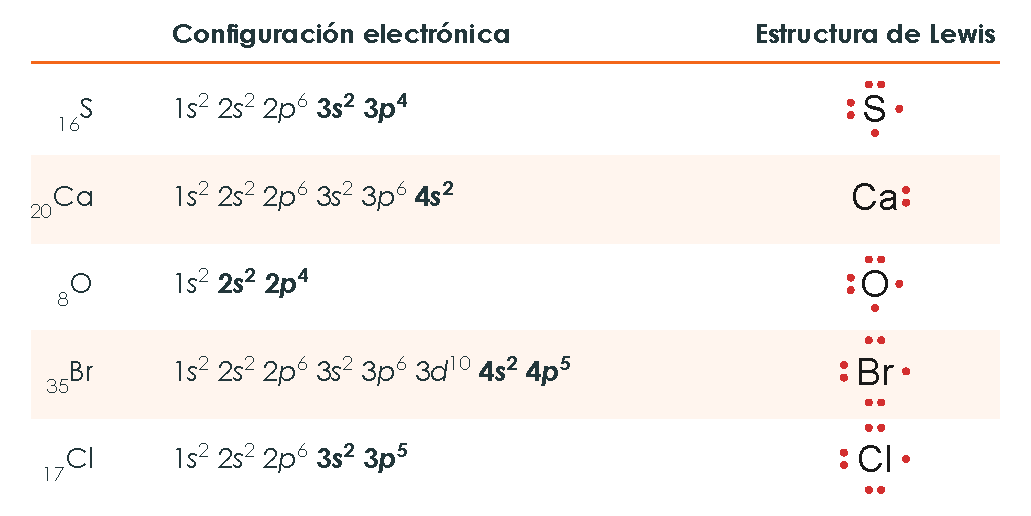
\includegraphics[width=0.62\textwidth]{images/UD4/lewis_atomos}
    \caption{Configuración electrónica y diagrama de Lewis de algunos átomos: solo se dibujan los electrones de la capa de valencia.}
    \label{fig:ud4-lewis-atomos}
\end{figure}

\paragraph{El ion más probable.} Con la regla del octeto podemos predecir qué ion formará un elemento: perderá o ganará los
electrones necesarios para quedar con la configuración del gas noble más cercano. Los metales, con pocos electrones de valencia,
los \textbf{pierden} y forman \textbf{cationes}; los no metales, con cinco, seis o siete, \textbf{ganan} los que les faltan y
forman \textbf{aniones}.

\begin{example}
    \textbf{Predecir iones.} ¿Qué ion tenderán a formar el magnesio (\(Z = 12\)) y el nitrógeno (\(Z = 7\))?

    \textbf{Solución.} Mg: \conf{1s^2\,2s^2\,2p^6\,3s^2}. Tiene 2 electrones de valencia: le es mucho más fácil perderlos que ganar
    seis, y queda con la configuración del neón: \(\ch{Mg} \rightarrow \ch{Mg^2+} + 2\,e^-\).

    N: \conf{1s^2\,2s^2\,2p^3}. Tiene 5 electrones de valencia y le faltan 3 para el octeto: tiende a ganarlos y formar el ion
    \ch{N^3-} (nitruro), también con la configuración del neón: \(\ch{N} + 3\,e^- \rightarrow \ch{N^3-}\).
\end{example}

\begin{remark}
    \textbf{Más allá del octeto.} Algunos elementos, sobre todo los de transición, no llegan a la configuración de gas noble,
    pero alcanzan una estabilidad especial con \textbf{subniveles llenos} (\conf{(n-1)d^{10}\,ns^2}, como el \ch{Zn^2+} con
    \conf{3d^{10}}) o \textbf{semillenos} (\conf{(n-1)d^5}, como el \ch{Fe^3+} o el \ch{Mn^2+}). Por eso el hierro forma
    \ch{Fe^2+} y \ch{Fe^3+}.
\end{remark}

\subsection{Tipos de enlace}

Los átomos pueden conseguir la configuración de gas noble de tres maneras: \textbf{cediendo}, \textbf{captando} o
\textbf{compartiendo} electrones. Según el tipo de elementos que se unen, hay tres tipos de enlace, y el tipo de enlace determina
las \textbf{propiedades} de la sustancia: puntos de fusión y ebullición, dureza, solubilidad, conductividad, brillo…

\begin{table}[H]
    \centering
    \caption{Los tres tipos de enlace químico}
    \vspace{-5pt}
    \begin{tabular}{@{}L{2cm}L{3cm}L{4.2cm}L{4.2cm}@{}}
        \toprule
        \textbf{Enlace} & \textbf{Entre} & \textbf{Qué ocurre} & \textbf{Qué se forma} \\
        \midrule
        Iónico & Metal y no metal & El metal cede electrones al no metal: se forman iones que se atraen & Una red cristalina de
        cationes y aniones (\ch{NaCl}) \\[3pt]
        Metálico & Átomos de un metal & Los átomos ceden sus electrones de valencia a una nube común & Una red de cationes
        rodeada de electrones (\ch{Cu}, \ch{Fe}) \\[3pt]
        Covalente & No metales & Los átomos comparten pares de electrones & Moléculas (\ch{H2O}, \ch{CO2}) o redes de átomos,
        los cristales covalentes (diamante, \ch{SiO2}) \\
        \bottomrule
    \end{tabular}
    \label{tab:ud4-tipos}
\end{table}

\begin{exercise}
    Predice el ion más probable que formarán el calcio, el fósforo, el potasio y el selenio. Escribe la configuración electrónica
    de cada átomo y de su ion.
    \begin{solu}
        Ca: \conf{[Ar]\,4s^2} \(\rightarrow\) \textcolor{red}{\ch{Ca^2+}}: \conf{[Ar]}. P: \conf{[Ne]\,3s^2\,3p^3} \(\rightarrow\)
        \textcolor{red}{\ch{P^3-}}: \conf{[Ne]\,3s^2\,3p^6} = \conf{[Ar]}. K: \conf{[Ar]\,4s^1} \(\rightarrow\)
        \textcolor{red}{\ch{K+}}: \conf{[Ar]}. Se: \conf{[Ar]\,3d^{10}\,4s^2\,4p^4} \(\rightarrow\) \textcolor{red}{\ch{Se^2-}}:
        \conf{[Ar]\,3d^{10}\,4s^2\,4p^6} = \conf{[Kr]}.
    \end{solu}
\end{exercise}

\begin{exercise}
    Con la tabla~\ref{tab:ud4-tipos}, predice qué tipo de enlace hay en: \ch{SO2}, \ch{Al}, \ch{CaBr2}, \ch{Ne} y \ch{H2S}.
    \begin{solu}
        \ch{SO2}: \textcolor{red}{covalente} (dos no metales). \ch{Al}: \textcolor{red}{metálico}. \ch{CaBr2}:
        \textcolor{red}{iónico} (metal y no metal). \ch{Ne}: \textcolor{red}{ninguno}: es un gas noble y existe como átomos sueltos.
        \ch{H2S}: \textcolor{red}{covalente}.
    \end{solu}
\end{exercise}

\begin{exercise}
    ¿Por qué el hidrógeno, el litio y el berilio no cumplen la regla del octeto? ¿Qué regla siguen?
    \begin{solu}
        \textcolor{red}{Su capa de valencia es la primera o la segunda y el gas noble más cercano es el helio}, que solo tiene dos
        electrones (\conf{1s^2}). Siguen la \textcolor{red}{«regla del dúo»}: el H gana o comparte un electrón (\ch{H-}, \ch{H2}) y
        el Li y el Be pierden 1 y 2 electrones (\ch{Li+}, \ch{Be^2+}).
    \end{solu}
\end{exercise}

\begin{exercise}
    Dibuja el diagrama de Lewis de los átomos de boro, carbono, nitrógeno, azufre y yodo.
    \begin{solu}
        Electrones de valencia: B 3, C 4, N 5, S 6 y I 7:
        \textcolor{red}{\chemfig{\charge{0=\.,90=\.,180=\.}{B}} \quad \chemfig{\charge{0=\.,90=\.,180=\.,270=\.}{C}} \quad
        \chemfig{\charge{0=\.,90=\:,180=\.,270=\.}{N}} \quad \chemfig{\charge{0=\.,90=\:,180=\.,270=\:}{S}} \quad
        \chemfig{\charge{0=\.,90=\:,180=\:,270=\:}{I}}}.
    \end{solu}
\end{exercise}

%========================================================================================
\section{Enlace iónico}\label{sec:ud4-ionico}
%========================================================================================

Cuando se encuentran un \textbf{metal} y un \textbf{no metal}, el metal, con pocos electrones de valencia y energía de ionización
baja, los \textbf{pierde} y se convierte en un \textbf{catión}; el no metal, muy electronegativo, los \textbf{gana} y se convierte
en un \textbf{anión}. Los iones, de carga opuesta, se atraen.

\begin{definition}[Enlace iónico]
    Es la unión que resulta de la \textbf{atracción eléctrica} entre \textbf{cationes} y \textbf{aniones}, formados por
    \textbf{transferencia de electrones} de los átomos de un metal a los de un no metal.
\end{definition}

Fíjate en el cloruro de sodio. El sodio (\conf{1s^2\,2s^2\,2p^6\,3s^1}) pierde su único electrón de valencia y queda como
\ch{Na+}, con la configuración del neón. El cloro (\conf{1s^2\,2s^2\,2p^6\,3s^2\,3p^5}) capta ese electrón y queda como \ch{Cl-},
con la del argón:
\[ \ch{Na} \rightarrow \ch{Na+} + e^- \qquad\qquad \ch{Cl} + e^- \rightarrow \ch{Cl-} \]
La figura~\ref{fig:ud4-lewis-iones} muestra el mismo proceso para el fluoruro de sodio con diagramas de Lewis.

\begin{figure}[H]
    \centering
    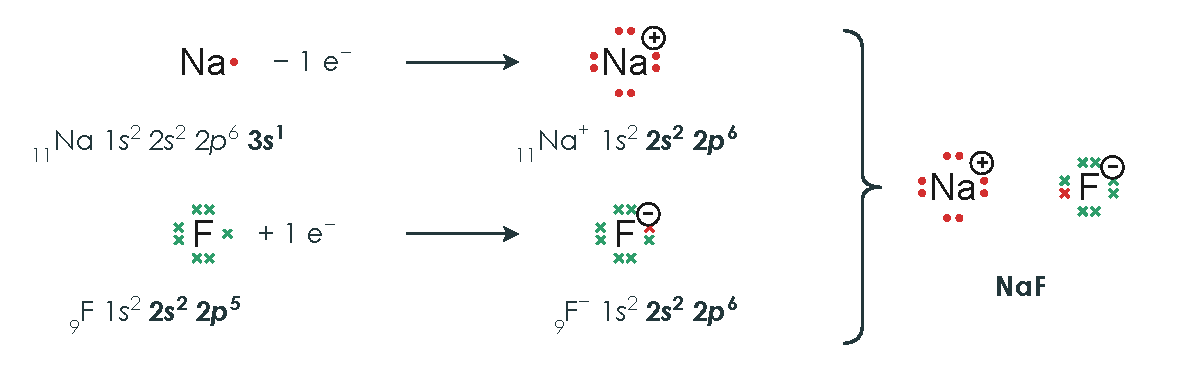
\includegraphics[width=0.62\textwidth]{images/UD4/lewis_iones}
    \caption{Formación del fluoruro de sodio: el sodio cede su electrón de valencia al flúor.}
    \label{fig:ud4-lewis-iones}
\end{figure}

\paragraph{Fórmula de un compuesto iónico.} El compuesto tiene que ser \textbf{neutro}: tiene que haber tantas cargas positivas
como negativas. La fórmula indica la \textbf{proporción} en que están los iones:
\begin{itemize}
    \item En el \ch{NaCl} hay un \ch{Na+} por cada \ch{Cl-}.
    \item En el \ch{CaF2}, dos \ch{F-} por cada \ch{Ca^2+}.
    \item En el \ch{Al2O3}, dos \ch{Al^3+} (6 cargas positivas) por cada tres \ch{O^2-} (6 cargas negativas).
\end{itemize}

\begin{remark}
    \textbf{No hay moléculas de \ch{NaCl}.} La fórmula de un compuesto iónico es una \textbf{fórmula empírica}: solo indica la
    proporción de iones en el cristal. Por eso no se habla de masa molecular, sino de \textbf{masa fórmula}: la del \ch{NaCl} es
    \(\num{23.0} + \num{35.5} = \qty{58.5}{\uma}\), y su masa molar, \qty{58.5}{\gram\per\mol}.
\end{remark}

\subsection{Redes iónicas}

Los iones no se unen por parejas: cada ion atrae a \textbf{todos} los iones de signo contrario que tiene alrededor, y se rodea del
mayor número posible de ellos. Así se forma una estructura gigante, ordenada y que se repite en las tres direcciones del espacio:
una \textbf{red cristalina} o \textbf{cristal}.

En la red, los iones se colocan de la forma más \textbf{compacta} posible, con la máxima distancia entre los iones del mismo signo y
la mínima entre los de signo contrario. El número de iones de signo contrario que rodean a cada ion es el \textbf{índice de
coordinación}, y depende de la proporción entre cationes y aniones y de su \textbf{tamaño} (figura~\ref{fig:ud4-redes}).

\begin{figure}[H]
    \centering
    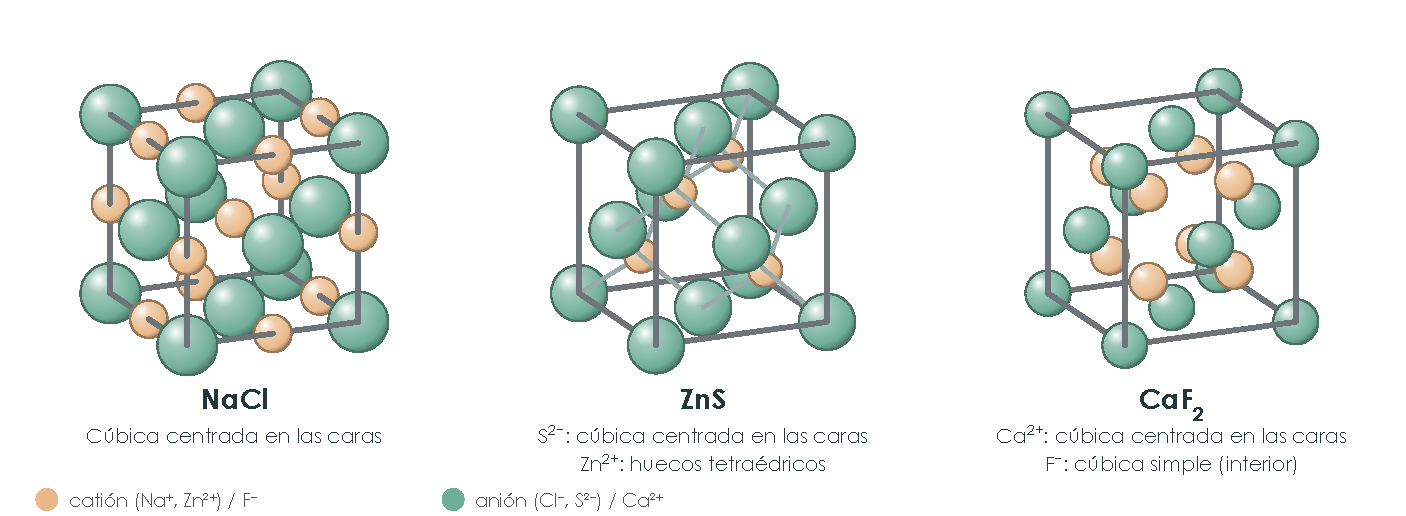
\includegraphics[width=0.85\textwidth]{images/UD4/redes_ionicas}
    \caption{Tres redes iónicas. En el \ch{NaCl} cada ion está rodeado por 6 de signo contrario; en la fluorita (\ch{CaF2}),
    cada \ch{Ca^2+} por 8 \ch{F-} y cada \ch{F-} por 4 \ch{Ca^2+}. En el \ch{CsCl} (no dibujado), el índice es 8 para los dos iones.}
    \label{fig:ud4-redes}
\end{figure}

\subsection{La energía reticular}

La formación de un cristal iónico a partir de sus elementos se puede imaginar como una serie de pasos, unos que absorben energía y
otros que la desprenden. Para el cloruro de sodio, partiendo de sodio sólido y cloro gaseoso
(tabla~\ref{tab:ud4-born-haber} y figura~\ref{fig:ud4-born-haber}):

\begin{table}[H]
    \centering
    \caption{Etapas de la formación del cloruro de sodio (ciclo de Born-Haber)}
    \vspace{-5pt}
    \begin{tabular}{@{}clL{5.2cm}r@{}}
        \toprule
        & \textbf{Etapa} & \textbf{Proceso} & \textbf{Energía (\unit{\kilo\joule\per\mol})} \\
        \midrule
        1 & Sublimar el sodio & \(\ch{Na(s)} \rightarrow \ch{Na(g)}\) & \(+108\) \\[3pt]
        2 & Disociar el cloro & \(\tfrac{1}{2}\,\ch{Cl2(g)} \rightarrow \ch{Cl(g)}\) & \(+121\) \\[3pt]
        3 & Ionizar el sodio & \(\ch{Na(g)} \rightarrow \ch{Na^+(g)} + e^-\) & \(+496\) \\[3pt]
        4 & El cloro capta un electrón & \(\ch{Cl(g)} + e^- \rightarrow \ch{Cl^-(g)}\) & \(-349\) \\[3pt]
        5 & Formar la red cristalina & \(\ch{Na^+(g)} + \ch{Cl^-(g)} \rightarrow \ch{NaCl(s)}\) & \(-787\) \\
        \midrule
        & \textbf{Proceso global} & \(\ch{Na(s)} + \tfrac{1}{2}\,\ch{Cl2(g)} \rightarrow \ch{NaCl(s)}\) & \(\mathbf{-411}\) \\
        \bottomrule
    \end{tabular}
    \label{tab:ud4-born-haber}
\end{table}

\begin{figure}[H]
    \centering
    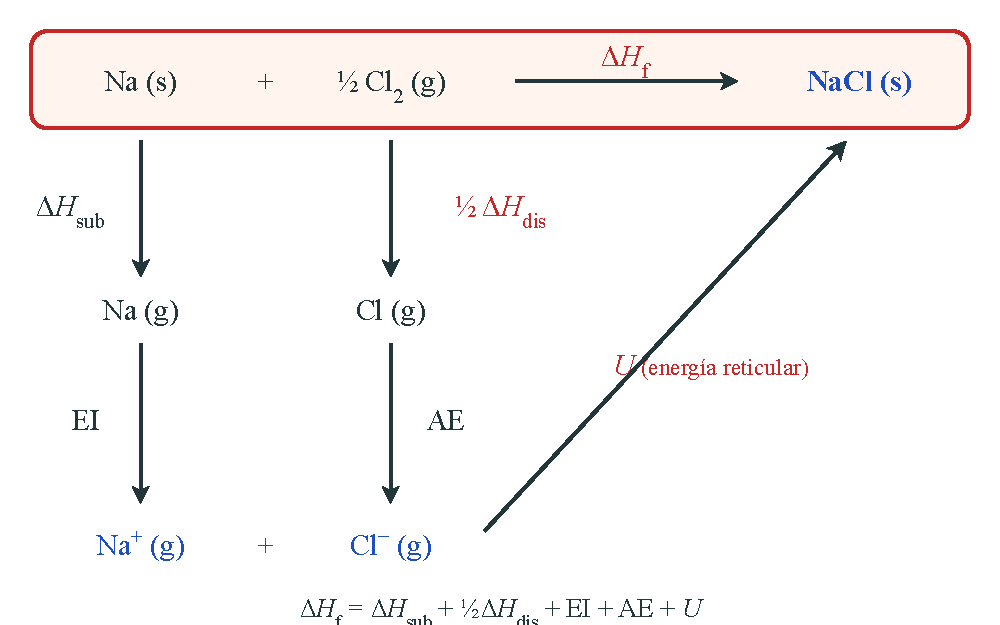
\includegraphics[width=0.62\textwidth]{images/UD4/born_haber}
    \caption{Ciclo de Born-Haber del cloruro de sodio: el camino directo (arriba) y el camino por etapas desprenden la misma
    energía. EI es la energía de ionización; AE, la afinidad electrónica, y \(U\), la energía reticular.}
    \label{fig:ud4-born-haber}
\end{figure}

Las tres primeras etapas \textbf{absorben} energía, y la cuarta desprende algo menos que lo que costó ionizar el sodio: si todo
acabara ahí, formar iones sueltos no saldría a cuenta. Lo que hace que el proceso global desprenda energía es la última etapa: la
unión de los iones gaseosos para formar el cristal.

\begin{definition}[Energía reticular]
    Es la energía que se \textbf{desprende} al formarse un mol de cristal iónico a partir de sus iones en estado gaseoso. Cuanto
    mayor es (en valor absoluto), más estable es el cristal. Es mayor cuanto \textbf{mayor} es la \textbf{carga} de los iones y
    cuanto \textbf{menor} es su \textbf{tamaño}, como predice la ley de Coulomb.
\end{definition}

\begin{example}
    \textbf{¿Cuál tiene mayor energía reticular?} Ordena de mayor a menor energía reticular (en valor absoluto) el \ch{NaCl}, el
    \ch{KCl} y el \ch{MgO}.

    \textbf{Solución.} El \ch{MgO} está formado por iones de carga \(+2\) y \(-2\), pequeños: la atracción entre ellos es unas
    cuatro veces mayor que entre iones de carga \(\pm 1\). Entre el \ch{NaCl} y el \ch{KCl}, el anión es el mismo y el \ch{Na+} es
    más pequeño que el \ch{K+} (tiene una capa menos), así que los iones quedan más cerca:
    \(\ch{MgO} > \ch{NaCl} > \ch{KCl}\). Los valores reales son \num{3850}, 787 y \qty{717}{\kilo\joule\per\mol}. Por eso el
    \ch{MgO} funde a \qty{2852}{\degreeCelsius} y el \ch{NaCl} a \qty{801}{\degreeCelsius}.
\end{example}

\begin{example}
    \textbf{Ciclo de Born-Haber del bromuro de potasio.} Calcula la energía que se desprende al formarse un mol de \ch{KBr(s)} a
    partir de sus elementos con estos datos (en \unit{\kilo\joule\per\mol}): sublimación del K, \(+89\); vaporización y disociación
    de medio mol de \ch{Br2(l)}, \(+112\); ionización del K, \(+419\); afinidad electrónica del Br, \(-325\); energía reticular del
    \ch{KBr}, \(-689\).

    \textbf{Solución.} La energía del proceso global es la suma de la de todas las etapas, porque la energía no depende del camino:
    \[ E = 89 + 112 + 419 - 325 - 689 = \qty{-394}{\kilo\joule\per\mol} \]
    Se desprenden \qty{394}{\kilo\joule} por mol de \ch{KBr} formado.
\end{example}

\subsection{Propiedades de los compuestos iónicos}

Las propiedades de los compuestos iónicos se deben a las fuerzas eléctricas, muy intensas, entre iones de distinto signo, que se
reflejan en el alto valor de su energía reticular:
\begin{itemize}
    \item Son \textbf{sólidos} a temperatura ambiente y tienen \textbf{puntos de fusión y ebullición altos}: para fundirlos hay que
    vencer la atracción entre los iones de toda la red.
    \item Son \textbf{duros}: para rayarlos hay que romper muchas atracciones entre los iones de la superficie.
    \item Son \textbf{frágiles}: al golpearlos, una capa de iones se desplaza sobre otra y quedan enfrentados iones del mismo
    signo, que se repelen y parten el cristal (figura~\ref{fig:ud4-deformacion}).
    \item Muchos son \textbf{solubles en agua} (y en otros disolventes polares): las moléculas de agua, que son dipolos, rodean a los
    iones de la superficie y los arrancan del cristal (figura~\ref{fig:ud4-disolucion}). Son insolubles en disolventes apolares.
    \item \textbf{No conducen la electricidad en estado sólido}, porque los iones no se pueden mover, pero \textbf{sí la conducen
    fundidos o disueltos}, cuando los iones quedan libres.
\end{itemize}

\begin{figure}[H]
    \centering
    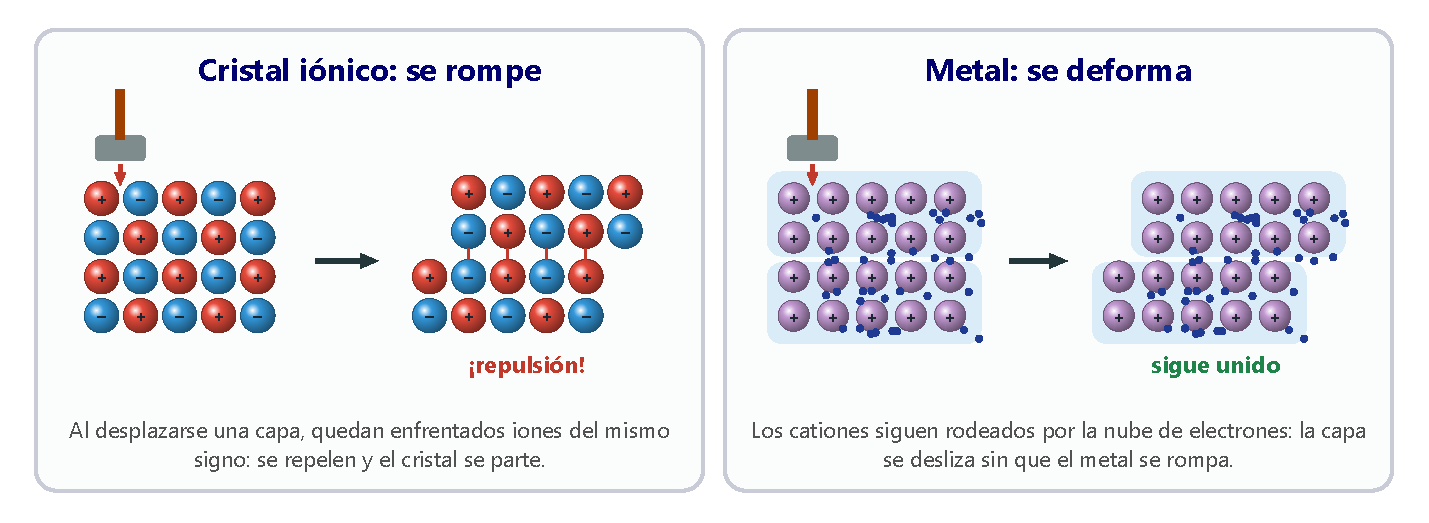
\includegraphics[width=0.85\textwidth]{images/UD4/deformacion}
    \caption{Un golpe rompe un cristal iónico, pero solo deforma un metal.}
    \label{fig:ud4-deformacion}
\end{figure}

\begin{figure}[H]
    \centering
    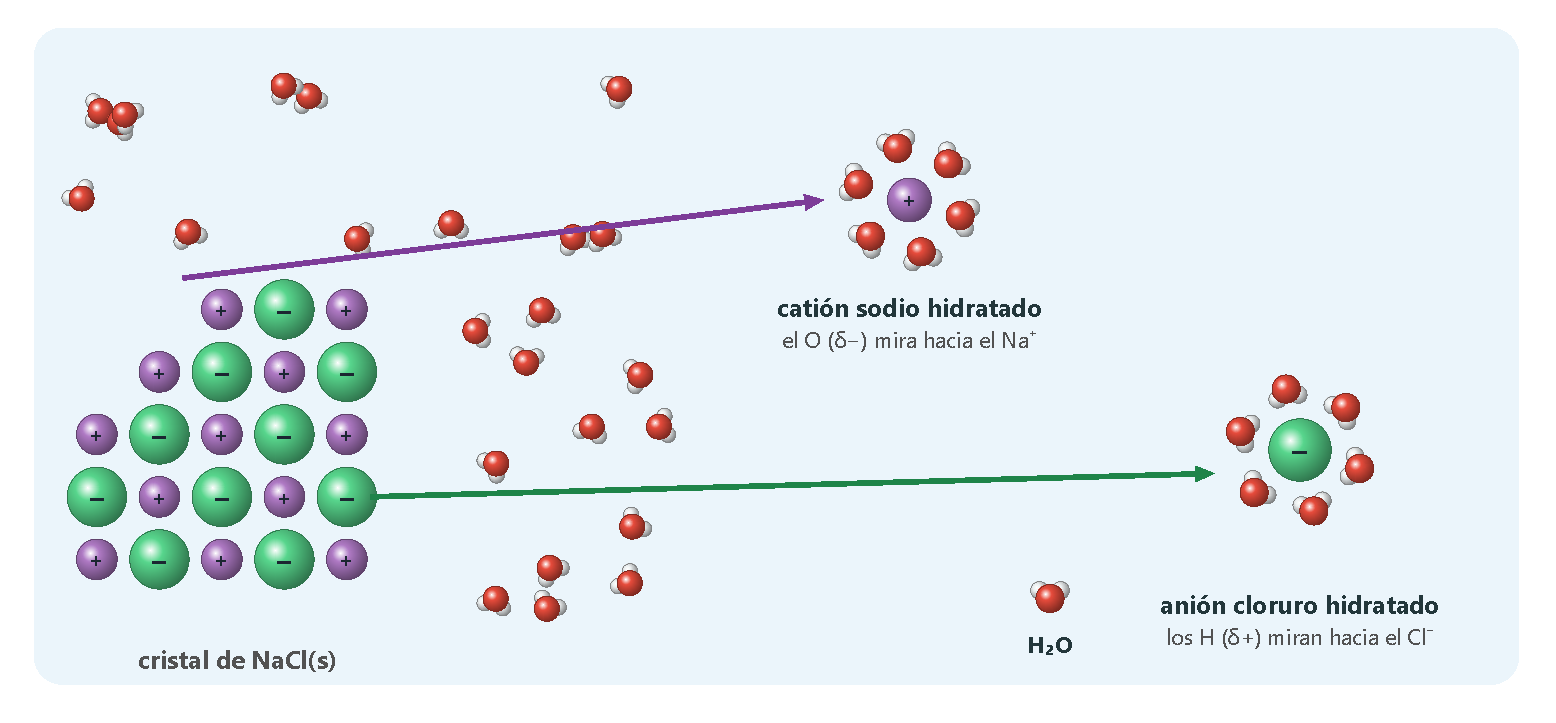
\includegraphics[width=0.8\textwidth]{images/UD2/disolucion_nacl}
    \caption{Disolución de un cristal iónico en agua: los iones quedan rodeados de moléculas de agua (iones hidratados).}
    \label{fig:ud4-disolucion}
\end{figure}

\begin{example}
    \textbf{Cómo se forma el yoduro de potasio.} Explica la formación del enlace en el \ch{KI}.

    \textbf{Solución.} El potasio es un metal y el yodo un no metal: el enlace es iónico. El K pierde su electrón 4s y el I lo
    gana, y los dos quedan con configuración de gas noble:
    \[ \ch{K}: \conf{[Ar]\,4s^1} \xrightarrow{\;-1\,e^-\;} \ch{K+}: \conf{[Ar]} \qquad\qquad
    \ch{I}: \conf{[Kr]\,4d^{10}\,5s^2\,5p^5} \xrightarrow{\;+1\,e^-\;} \ch{I-}: \conf{[Kr]\,4d^{10}\,5s^2\,5p^6} = \conf{[Xe]} \]
    Los iones \ch{K+} y \ch{I-} se atraen y se ordenan en una red cristalina en la que hay un \ch{K+} por cada \ch{I-}: \ch{KI}.
\end{example}

\begin{exercise}
    Explica cómo se forma el enlace en estos compuestos y justifica su fórmula: a) \ch{MgBr2}; b) \ch{Na2S}; c) \ch{CaO}.
    \begin{solu}
        a) \ch{Mg} \(\rightarrow\) \ch{Mg^2+} \(+\, 2\,e^-\); cada Br capta un electrón: \(\ch{Br} + e^- \rightarrow \ch{Br-}\).
        \textcolor{red}{Hacen falta dos \ch{Br-} por cada \ch{Mg^2+}}. b) Cada Na pierde un electrón y el S gana dos:
        \textcolor{red}{dos \ch{Na+} por cada \ch{S^2-}}. c) El Ca pierde dos electrones y el O gana dos:
        \textcolor{red}{un \ch{Ca^2+} por cada \ch{O^2-}}. En los tres casos los iones quedan con configuración de gas noble y
        se atraen formando una red cristalina.
    \end{solu}
\end{exercise}

\begin{exercise}
    Calcula la masa fórmula del \ch{CaCl2} y del \ch{Al2O3} (masas atómicas: Ca 40,1; Cl 35,5; Al 27,0; O 16,0). ¿Por qué no
    hablamos de masa molecular?
    \begin{solu}
        \ch{CaCl2}: \(\num{40.1} + 2 \cdot \num{35.5} = \textcolor{red}{\qty{111.1}{\uma}}\). \ch{Al2O3}:
        \(2 \cdot \num{27.0} + 3 \cdot \num{16.0} = \textcolor{red}{\qty{102.0}{\uma}}\). \textcolor{red}{Porque los compuestos
        iónicos no forman moléculas}: son redes de iones y su fórmula solo indica la proporción entre ellos.
    \end{solu}
\end{exercise}

\begin{exercise}
    Calcula la energía reticular del fluoruro de litio sabiendo que en su formación a partir de sus elementos se desprenden
    \qty{616}{\kilo\joule\per\mol} y que (en \unit{\kilo\joule\per\mol}): sublimación del Li, \(+159\); disociación de medio mol de
    \ch{F2}, \(+79\); ionización del Li, \(+520\); afinidad electrónica del F, \(-328\).
    \begin{solu}
        \(-616 = 159 + 79 + 520 - 328 + U \;\Rightarrow\; U = -616 - 430 = \textcolor{red}{\qty{-1046}{\kilo\joule\per\mol}}\).
        Es mucho mayor que la del \ch{NaCl}, porque el \ch{Li+} y el \ch{F-} son iones muy pequeños.
    \end{solu}
\end{exercise}

\begin{exercise}
    Ordena de mayor a menor punto de fusión: \ch{NaF}, \ch{NaBr}, \ch{CaO} y \ch{NaCl}. Justifica la respuesta.
    \begin{solu}
        El punto de fusión crece con la energía reticular, que aumenta con la carga de los iones y al disminuir su tamaño.
        El \ch{CaO} tiene iones de carga \(\pm 2\); los otros tres tienen el mismo catión y aniones cada vez mayores
        (\(\ch{F-} < \ch{Cl-} < \ch{Br-}\)): \textcolor{red}{\(\ch{CaO} > \ch{NaF} > \ch{NaCl} > \ch{NaBr}\)} (2613, 993, 801 y
        \qty{747}{\degreeCelsius}).
    \end{solu}
\end{exercise}

\begin{exercise}
    Al cocinar, solemos manejar un salero de vidrio. Si se nos cae al suelo, la sal no se dobla ni se aplasta: los granos se
    rompen en trocitos con caras planas. ¿Por qué? ¿Y por qué no conviene manejar aparatos eléctricos con las manos mojadas, si el
    agua pura apenas conduce la corriente?
    \begin{solu}
        \textcolor{red}{Los cristales iónicos son frágiles}: el golpe desplaza capas de iones, quedan enfrentados iones del mismo
        signo y el cristal se rompe por esos planos, que son planos. \textcolor{red}{El agua del grifo y el sudor llevan sales
        disueltas}: sus iones, libres para moverse, la hacen conductora.
    \end{solu}
\end{exercise}

%========================================================================================
\section{Enlace metálico}\label{sec:ud4-metalico}
%========================================================================================

Un trozo de cobre o de hierro, por pequeño que sea, contiene una cantidad enorme de átomos iguales. ¿Qué los mantiene unidos? Los
metales son densos, lo que indica que sus átomos están muy apretados, y conducen muy bien la electricidad, lo que exige que haya
cargas que se puedan mover. El modelo de la \textbf{nube electrónica} (o del \textbf{mar de electrones}) explica las dos cosas a
partir de dos características de los metales:
\begin{itemize}
    \item Tienen \textbf{energías de ionización bajas}: cuesta poco arrancarles electrones.
    \item Tienen \textbf{pocos electrones} de valencia (uno, dos o tres).
\end{itemize}

Según este modelo, cada átomo del metal cede sus electrones de valencia y se convierte en un \textbf{catión}. Los electrones
liberados no pertenecen a ningún átomo concreto: forman un \textbf{colectivo deslocalizado}, una nube que rodea a todos los
cationes y se mueve libremente entre ellos. Los cationes se ordenan en una \textbf{red cristalina compacta}
(figura~\ref{fig:ud4-nube}).

\begin{figure}[H]
    \centering
    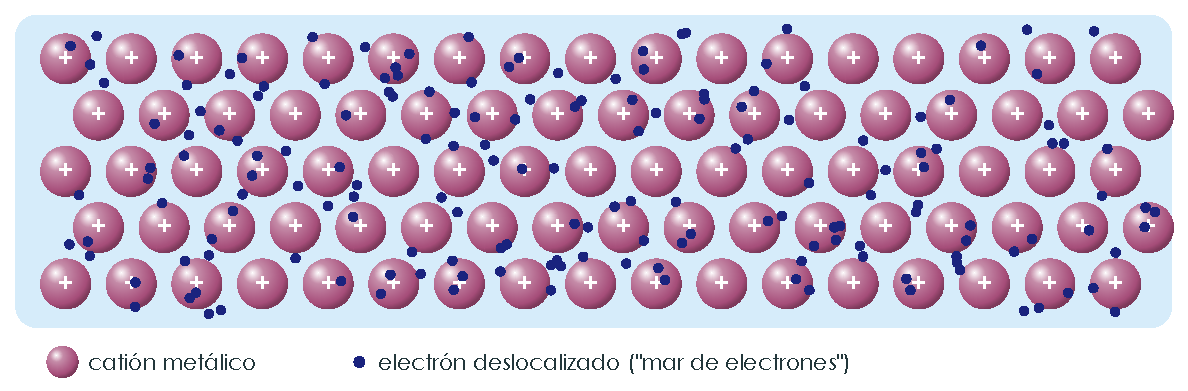
\includegraphics[width=0.6\textwidth]{images/UD4/nube_electronica}
    \caption{Modelo de la nube electrónica: cationes ordenados en una red, rodeados de electrones deslocalizados.}
    \label{fig:ud4-nube}
\end{figure}

\begin{definition}[Enlace metálico]
    Es la unión que resulta de la \textbf{atracción eléctrica} entre los \textbf{cationes} de la red y la \textbf{nube de
    electrones} deslocalizados que los rodea.
\end{definition}

\begin{example}
    \textbf{Electrones que aporta cada metal.} ¿Cuántos electrones cede a la nube electrónica un átomo de sodio y uno de aluminio?

    \textbf{Solución.} Cada metal cede los electrones de su capa de valencia:
    \[ \ch{Na}: \conf{[Ne]\,3s^1} \xrightarrow{\;-1\,e^-\;} \ch{Na+}: \conf{[Ne]} \qquad\qquad
    \ch{Al}: \conf{[Ne]\,3s^2\,3p^1} \xrightarrow{\;-3\,e^-\;} \ch{Al^3+}: \conf{[Ne]} \]
    El sodio cede \textbf{un} electrón y el aluminio, \textbf{tres}. Con más electrones en la nube y cationes de mayor carga, el
    enlace metálico del aluminio es más fuerte: funde a \qty{660}{\degreeCelsius}, frente a los \qty{98}{\degreeCelsius} del sodio.
\end{example}

\subsection{Propiedades de los metales}

\begin{itemize}
    \item Salvo el mercurio, que funde a \qty{-39}{\degreeCelsius}, son \textbf{sólidos} a temperatura ambiente. Sus puntos de
    fusión son muy variados: desde los \qty{29}{\degreeCelsius} del galio, que se funde en la mano, hasta los
    \qty{3422}{\degreeCelsius} del wolframio.
    \item Tienen \textbf{densidad alta}, porque la red de cationes es muy compacta.
    \item Son \textbf{dúctiles} (se estiran en hilos) y \textbf{maleables} (se extienden en láminas): cuando una capa de cationes
    se desliza sobre otra, la nube electrónica se adapta y sigue uniéndolos, sin que aparezcan repulsiones
    (figura~\ref{fig:ud4-deformacion}).
    \item Son \textbf{buenos conductores de la electricidad y del calor}, gracias a la movilidad de los electrones de la nube.
    \item Tienen un \textbf{brillo} característico: los electrones libres absorben la luz y la vuelven a emitir.
    \item Son \textbf{insolubles} en agua y en los disolventes habituales (algunos, como los alcalinos, reaccionan con el agua, que
    no es lo mismo). Fundidos se mezclan entre sí y forman \textbf{aleaciones}, como el bronce (cobre y estaño) o el latón (cobre y
    cinc). El acero es hierro con un poco de carbono.
\end{itemize}

\begin{remark}
    \textbf{Conductores, semiconductores y aislantes.} Un modelo más completo, la \textbf{teoría de bandas}, explica la conducción
    con los niveles de energía de los electrones del cristal (figura~\ref{fig:ud4-bandas}). En un conductor, la banda que ocupan
    los electrones de valencia se solapa con una banda vacía (de conducción) a la que los electrones pasan sin esfuerzo. En un
    aislante, entre ambas hay un gran salto de energía. En un \textbf{semiconductor}, como el silicio, el salto es pequeño: con un
    poco de energía (calor o luz) algunos electrones lo superan y el material conduce, y con ellos se fabrican los chips y las
    placas solares.
\end{remark}

\begin{figure}[H]
    \centering
    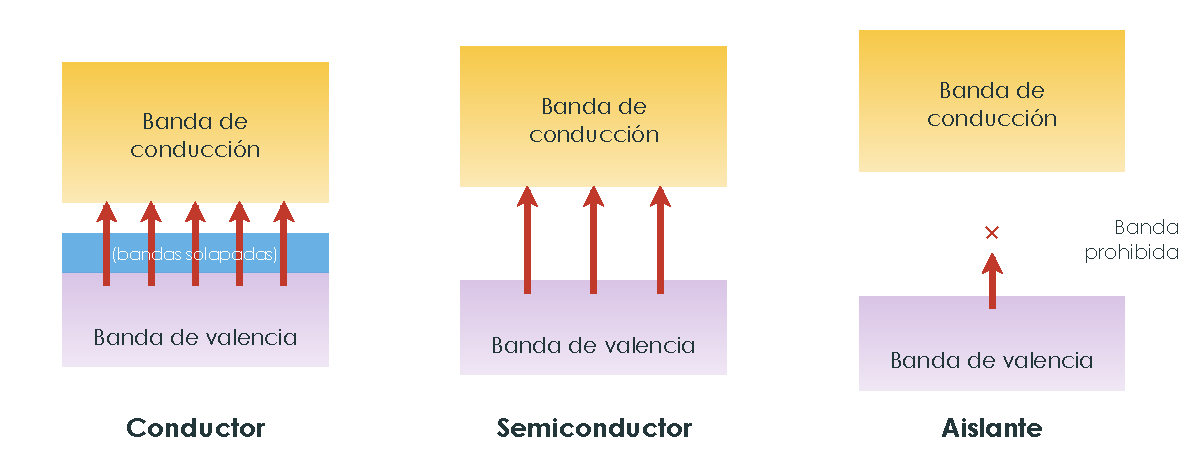
\includegraphics[width=0.65\textwidth]{images/UD4/bandas}
    \caption{Teoría de bandas: conductores, semiconductores y aislantes.}
    \label{fig:ud4-bandas}
\end{figure}

\begin{exercise}
    ¿Cuántos electrones cede a la nube electrónica un átomo de cada uno de estos metales? a) Li; b) Ca; c) Ga; d) Ba.
    \begin{solu}
        Cada uno cede sus electrones de valencia: a) Li, \conf{[He]\,2s^1}: \textcolor{red}{1}. b) Ca, \conf{[Ar]\,4s^2}:
        \textcolor{red}{2}. c) Ga, \conf{[Ar]\,3d^{10}\,4s^2\,4p^1}: \textcolor{red}{3}. d) Ba, \conf{[Xe]\,6s^2}: \textcolor{red}{2}.
    \end{solu}
\end{exercise}

\begin{exercise}
    ¿Por qué podemos hacer cables de cobre o papel de aluminio, pero no podemos hacer hilos de sal común?
    \begin{solu}
        \textcolor{red}{Los metales son dúctiles y maleables}: al deformarlos, las capas de cationes se deslizan sin que la nube de
        electrones deje de unirlas. \textcolor{red}{La sal es frágil}: al deformarla, quedan enfrentados iones del mismo signo, que
        se repelen, y el cristal se rompe.
    \end{solu}
\end{exercise}

\begin{exercise}
    Las sartenes son de metal, pero sus mangos suelen ser de plástico o de madera. ¿Por qué?
    \begin{solu}
        \textcolor{red}{Los metales conducen muy bien el calor}, gracias a los electrones libres, y el mango se calentaría tanto
        como el fondo. \textcolor{red}{El plástico y la madera son malos conductores} (sus electrones están localizados en enlaces
        covalentes) y no queman.
    \end{solu}
\end{exercise}

\begin{exercise}
    El potasio funde a \qty{63}{\degreeCelsius} y el calcio, a \qty{842}{\degreeCelsius}. Explica la diferencia con el modelo de
    la nube electrónica.
    \begin{solu}
        \textcolor{red}{El K cede un electrón y queda como \ch{K+}; el Ca cede dos y queda como \ch{Ca^2+}}, más pequeño y con más
        carga. En el calcio la nube tiene el doble de electrones y la atracción entre la nube y los cationes es mucho mayor: hace
        falta más energía para romper la red.
    \end{solu}
\end{exercise}

%========================================================================================
\section{Enlace covalente}\label{sec:ud4-covalente}
%========================================================================================

Imagina que en clase de Lengua os mandan leer dos libros y en tu casa tenéis uno y en la de un amigo, el otro. Lo más sencillo es
que os los prestéis: cada uno usa los dos libros sin comprar ninguno. Algo parecido hacen los átomos de los no metales: todos
necesitan \textbf{ganar} electrones para completar su capa de valencia, y como ninguno quiere cederlos, los \textbf{comparten}.

Fíjate en el hidrógeno. Cada átomo de H tiene un electrón; si los dos átomos juntan sus electrones en un \textbf{par
compartido}, cada uno «tiene» dos electrones y alcanza la configuración del helio:
\[ \mathrm{H}\!\cdot \;+\; \cdot\mathrm{H} \;\longrightarrow\; \mathrm{H}\!:\!\mathrm{H} \quad \text{o bien} \quad \mathrm{H{-}H} \]
Del mismo modo, cada átomo de flúor, con siete electrones de valencia, comparte uno con el otro y los dos completan el octeto
(figura~\ref{fig:ud4-F2}).

\begin{figure}[H]
    \centering
    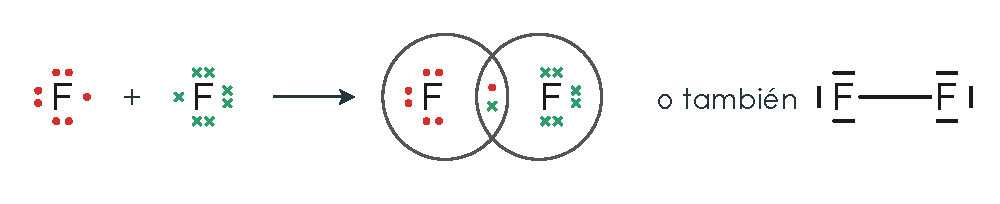
\includegraphics[width=0.55\textwidth]{images/UD4/lewis_F2}
    \caption{Formación de la molécula de flúor: el par compartido cuenta para el octeto de los dos átomos.}
    \label{fig:ud4-F2}
\end{figure}

\begin{definition}[Enlace covalente]
    Es la unión entre átomos que \textbf{comparten} uno o más \textbf{pares de electrones}, atraídos a la vez por los dos núcleos.
    Se da entre átomos de \textbf{no metales}.

    La \textbf{valencia covalente} (o covalencia) de un átomo es el número de enlaces covalentes que forma, y suele coincidir con el
    número de electrones que le faltan para completar el octeto (o con el de sus electrones desapareados).
\end{definition}

En una estructura de Lewis, cada \textbf{par compartido} o \textbf{par enlazante} se dibuja como un guion, y los pares que no se
comparten (\textbf{pares no enlazantes} o \textbf{solitarios}) se dibujan como dos puntos. En el agua, por ejemplo, el oxígeno
tiene 6 electrones de valencia y le faltan 2: comparte un par con cada hidrógeno y su valencia covalente es 2
(figura~\ref{fig:ud4-H2O}):
\[ \chemfig{H-\charge{90=\:,270=\:}{O}-H} \]

\begin{figure}[H]
    \centering
    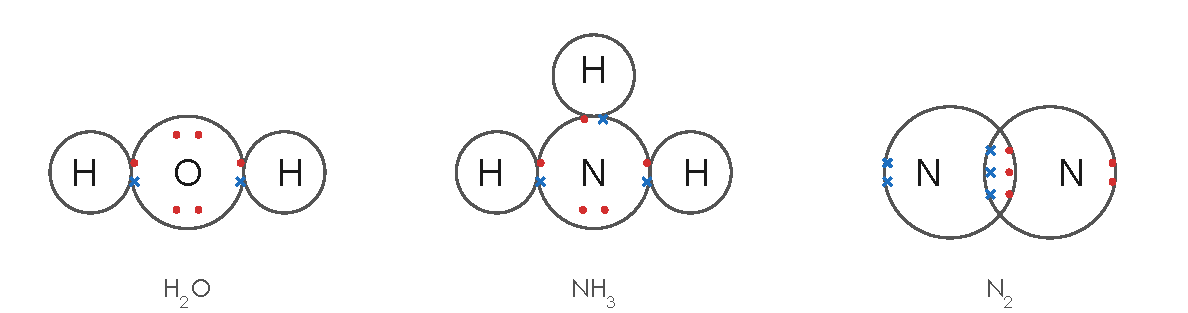
\includegraphics[width=0.62\textwidth]{images/UD4/lewis_H2O_NH3_N2}
    \caption{Pares compartidos en el agua, el amoníaco y el nitrógeno. En el \ch{N2} los átomos comparten tres pares.}
    \label{fig:ud4-H2O}
\end{figure}

\paragraph{Enlaces simples, dobles y triples.} Si los átomos comparten \textbf{un par} de electrones, el enlace es
\textbf{simple}; si comparten \textbf{dos}, es \textbf{doble}, y si comparten \textbf{tres}, \textbf{triple}:
\[ \chemfig{\charge{90=\:,180=\:,270=\:}{Cl}-\charge{0=\:,90=\:,270=\:}{Cl}} \qquad\qquad
\chemfig{\charge{90=\:,270=\:}{O}=\charge{90=\:,270=\:}{O}} \qquad\qquad
\chemfig{\charge{180=\:}{N}~\charge{0=\:}{N}} \]
Los enlaces múltiples son más cortos y más fuertes que los simples: la energía del enlace triple N\(\equiv\)N del nitrógeno es
\qty{945}{\kilo\joule\per\mol}, una de las más altas que se conocen, y por eso el \ch{N2} del aire es tan poco reactivo.

\paragraph{Enlace covalente dativo.} A veces los dos electrones del par compartido los aporta \textbf{uno solo} de los átomos, que
tiene un par solitario, y el otro átomo tiene un orbital vacío. Es lo que ocurre cuando el amoníaco capta un ion \ch{H+}, que no
tiene ningún electrón, y forma el ion amonio, \ch{NH4+} (figura~\ref{fig:ud4-dativo}). Una vez formado, el enlace dativo es igual
que los demás. A veces se dibuja como una flecha que va del átomo que aporta el par al que lo recibe.

\begin{figure}[H]
    \centering
    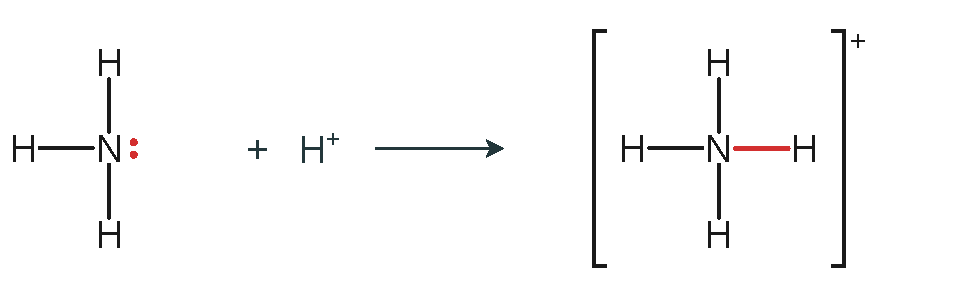
\includegraphics[width=0.55\textwidth]{images/UD4/dativo_amonio}
    \caption{Formación del ion amonio: el nitrógeno aporta los dos electrones del nuevo enlace (en rojo).}
    \label{fig:ud4-dativo}
\end{figure}

\subsection{Cómo escribir estructuras de Lewis}

Para moléculas sencillas, con un átomo central rodeado de otros, se puede seguir este método:
\begin{enumerate}[label=\numberballgreen]
    \item Se cuentan los electrones de valencia \textbf{disponibles}, \(D\), sumando los de todos los átomos (si es un ion, se
    suma un electrón por cada carga negativa o se resta uno por cada carga positiva).
    \item Se cuentan los electrones \textbf{necesarios}, \(N\), para que todos los átomos completen su capa: 8 por átomo y 2 por
    cada hidrógeno.
    \item Los electrones \textbf{compartidos} son \(C = N - D\), y el número de \textbf{enlaces} es \(C/2\).
    \item Se coloca en el centro el átomo menos electronegativo (nunca el H), se une a los demás con los enlaces calculados y se
    reparten los electrones restantes (\(D - C\)) como pares solitarios hasta completar los octetos.
\end{enumerate}

\begin{example}
    \textbf{Estructura de Lewis del \ch{CO2} y del \ch{HCN}.}

    \textbf{Solución.} \textbf{\ch{CO2}}: C (\conf{2s^2\,2p^2}) tiene 4 electrones de valencia y cada O (\conf{2s^2\,2p^4}), 6:
    \(D = 4 + 2 \cdot 6 = 16\). Necesarios: \(N = 3 \cdot 8 = 24\). Compartidos: \(C = 24 - 16 = 8\), es decir, \textbf{4
    enlaces}. El C va en el centro y forma un enlace doble con cada O; quedan \(16 - 8 = 8\) electrones, dos pares solitarios en
    cada O:
    \[ \chemfig{\charge{90=\:,270=\:}{O}=C=\charge{90=\:,270=\:}{O}} \]

    \textbf{\ch{HCN}}: \(D = 1 + 4 + 5 = 10\); \(N = 2 + 8 + 8 = 18\); \(C = 8\): \textbf{4 enlaces}. El C, en el centro, forma un
    enlace simple con el H y uno triple con el N; quedan \(10 - 8 = 2\) electrones, un par solitario en el N:
    \[ \chemfig{H-C~\charge{0=\:}{N}} \]
    Comprueba que el C tiene cuatro enlaces (valencia covalente 4), el N tres y el H uno.
\end{example}

\begin{example}
    \textbf{Formación de los enlaces del \ch{SCl2}.} Explica los enlaces del dicloruro de azufre.

    \textbf{Solución.} Escribimos las configuraciones electrónicas para ver cuántos electrones le faltan a cada átomo:
    S: \conf{[Ne]\,3s^2\,3p^4}, le faltan 2: valencia covalente 2. Cl: \conf{[Ne]\,3s^2\,3p^5}, le falta 1: valencia covalente 1.
    El azufre es el átomo central y comparte un par de electrones con cada cloro:
    \[ \chemfig{\charge{90=\:,180=\:,270=\:}{Cl}-\charge{90=\:,270=\:}{S}-\charge{0=\:,90=\:,270=\:}{Cl}} \]
\end{example}

\paragraph{Excepciones a la regla del octeto.} La regla del octeto falla en algunas moléculas (figura~\ref{fig:ud4-excepciones}):
\begin{itemize}
    \item \textbf{Octeto incompleto}: el boro y el aluminio, con 3 electrones de valencia, forman tres enlaces y se quedan con 6
    electrones (\ch{BF3}, \ch{BCl3}, \ch{AlCl3}); el berilio forma dos y se queda con 4 (\ch{BeCl2}).
    \item \textbf{Octeto expandido}: los elementos del tercer periodo y siguientes pueden rodearse de más de 8 electrones, porque
    disponen de orbitales \(d\) vacíos: el P en el \ch{PCl5} tiene 10 y el S en el \ch{SF6}, 12.
    \item \textbf{Número impar de electrones}: moléculas como el \ch{NO} (11 electrones de valencia) o el \ch{NO2} (17) tienen un
    electrón desapareado y no pueden completar el octeto de todos sus átomos. Se llaman \textbf{radicales} y son muy reactivas.
\end{itemize}

\begin{figure}[H]
    \centering
    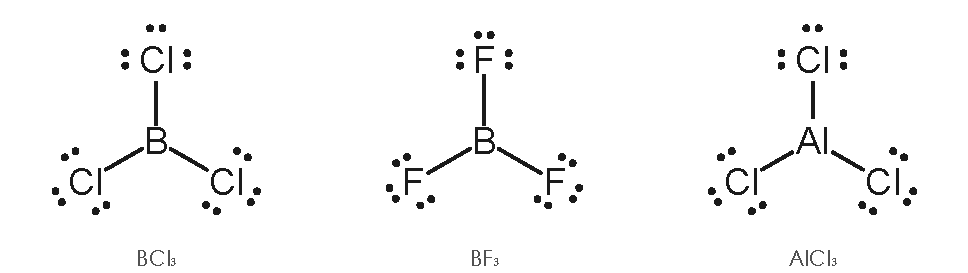
\includegraphics[width=0.45\textwidth]{images/UD4/octeto_incompleto}\hfill
    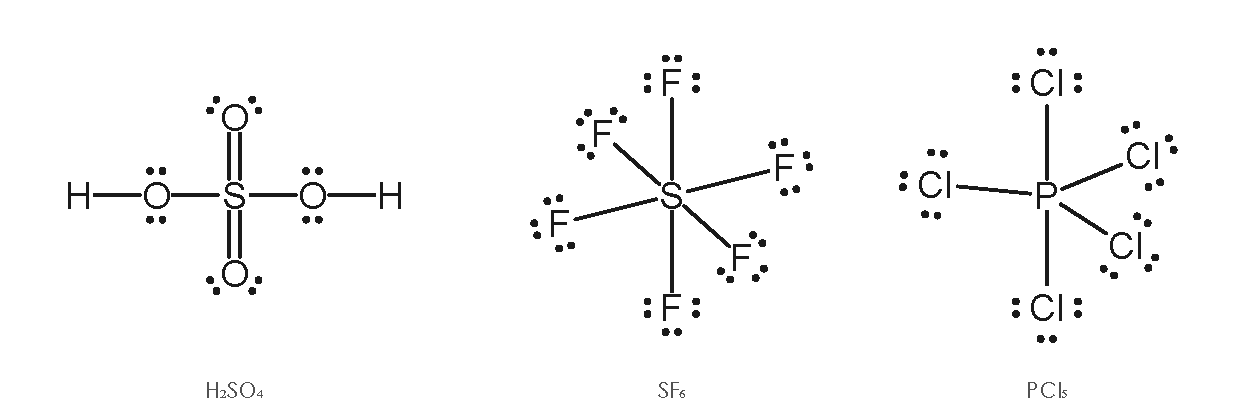
\includegraphics[width=0.45\textwidth]{images/UD4/octeto_ampliado}
    \caption{Excepciones a la regla del octeto: octeto incompleto (izquierda) y expandido (derecha).}
    \label{fig:ud4-excepciones}
\end{figure}

\paragraph{Energía y longitud de enlace.} La energía necesaria para romper un mol de enlaces covalentes en estado gaseoso es la
\textbf{energía de enlace}. Su valor depende de los átomos que se unen, pero en general es alto: el enlace covalente es un enlace
muy fuerte. Los enlaces dobles y triples son más fuertes y más cortos que los simples (tabla~\ref{tab:ud4-energias}).

\begin{table}[H]
    \centering
    \caption{Energía y longitud media de algunos enlaces covalentes}
    \vspace{-5pt}
    \begin{tabular}{@{}lcccccccc@{}}
        \toprule
        \textbf{Enlace} & H--H & C--H & O--H & C--C & C=C & C\(\equiv\)C & O=O & N\(\equiv\)N \\
        \midrule
        \textbf{Energía (\unit{\kilo\joule\per\mol})} & 436 & 413 & 463 & 347 & 614 & 839 & 498 & 945 \\[3pt]
        \textbf{Longitud (pm)} & 74 & 109 & 96 & 154 & 134 & 120 & 121 & 110 \\
        \bottomrule
    \end{tabular}
    \label{tab:ud4-energias}
\end{table}

\begin{exercise}
    Dibuja la estructura de Lewis del \ch{CO2}, el \ch{SiCl4} y el \ch{PH3}. Justifica en cada caso la valencia covalente de los
    átomos a partir de su configuración electrónica.
    \begin{solu}
        C: \conf{[He]\,2s^2\,2p^2}, valencia 4; O: \conf{[He]\,2s^2\,2p^4}, valencia 2;
        Si: \conf{[Ne]\,3s^2\,3p^2}, valencia 4; Cl: \conf{[Ne]\,3s^2\,3p^5}, valencia 1; P: \conf{[Ne]\,3s^2\,3p^3}, valencia 3;
        H: \conf{1s^1}, valencia 1.
        \begin{center}
            \textcolor{red}{\chemfig{\charge{90=\:,270=\:}{O}=C=\charge{90=\:,270=\:}{O}}} \qquad
            \textcolor{red}{\chemfig{Si(-[2]\charge{0=\:,90=\:,180=\:}{Cl})(-[4]\charge{90=\:,180=\:,270=\:}{Cl})(-[6]\charge{0=\:,180=\:,270=\:}{Cl})-\charge{0=\:,90=\:,270=\:}{Cl}}} \qquad
            \textcolor{red}{\chemfig{H-\charge{90=\:}{P}(-[6]H)-H}}
        \end{center}
    \end{solu}
\end{exercise}

\begin{exercise}
    Calcula, con el método de los electrones disponibles y necesarios, cuántos enlaces hay en el \ch{H2CO} (metanal) y dibuja su
    estructura de Lewis. ¿Qué tipo de enlace une el C con el O?
    \begin{solu}
        \(D = 2 \cdot 1 + 4 + 6 = 12\); \(N = 2 \cdot 2 + 8 + 8 = 20\); \(C = 8\): \textcolor{red}{4 enlaces}. El C, en el
        centro, se une a cada H con un enlace simple y al O con uno \textcolor{red}{doble}; quedan 4 electrones, dos pares
        solitarios en el O:
        \textcolor{red}{\chemfig{C(-[:150]H)(-[:210]H)=\charge{90=\:,270=\:}{O}}}.
    \end{solu}
\end{exercise}

\begin{exercise}
    El ion hidronio, \ch{H3O+}, se forma cuando una molécula de agua capta un ion \ch{H+}. Dibuja su estructura de Lewis e indica
    qué enlace es dativo y qué átomo aporta el par de electrones.
    \begin{solu}
        El oxígeno del agua tiene dos pares solitarios y \textcolor{red}{aporta uno de ellos} al \ch{H+}, que no tiene electrones:
        \textcolor{red}{el enlace O--H nuevo es dativo}. En el \ch{H3O+} el O tiene tres enlaces y un par solitario:
        \(\left[\,\chemfig{H-\charge{90=\:}{O}(-[6]H)-H}\,\right]^+\).
    \end{solu}
\end{exercise}

\begin{exercise}
    ¿Cumplen la regla del octeto el átomo central del \ch{BeF2}, del \ch{PF5} y del \ch{NO}? Justifícalo.
    \begin{solu}
        \textcolor{red}{No, ninguno.} \ch{BeF2}: el Be forma dos enlaces y queda con 4 electrones (octeto incompleto).
        \ch{PF5}: el P forma cinco enlaces y queda con 10 (octeto expandido, posible porque está en el periodo 3).
        \ch{NO}: tiene \(5 + 6 = 11\) electrones de valencia, un número impar: uno de los átomos queda con un electrón desapareado.
    \end{solu}
\end{exercise}

\subsection{Polaridad del enlace covalente}

Si los dos átomos que comparten electrones son \textbf{iguales} (\ch{H2}, \ch{Cl2}, \ch{O2}), atraen con la misma fuerza a los
electrones del enlace, que quedan repartidos por igual: la nube electrónica es \textbf{simétrica} y el enlace es \textbf{apolar}.

Si los átomos son \textbf{distintos}, el más \textbf{electronegativo} atrae con más intensidad a los electrones compartidos, y la
nube se desplaza hacia él. En el \ch{HCl}, el cloro (\(\mathrm{EN} = \num{3.2}\)) atrae el par más que el hidrógeno
(\(\mathrm{EN} = \num{2.2}\)): cerca del cloro hay un exceso de carga negativa, que se indica \(\delta^-\), y cerca del hidrógeno, un
déficit, \(\delta^+\). El enlace es \textbf{polar} y forma un pequeño \textbf{dipolo}:
\[ \overset{\delta^+}{\mathrm{H}}{-}\overset{\delta^-}{\mathrm{Cl}} \]

\begin{definition}[Polaridad del enlace]
    Un enlace covalente es \textbf{polar} cuando los átomos que lo forman tienen distinta electronegatividad. La polaridad es mayor
    cuanto mayor es la \textbf{diferencia de electronegatividad}, \(\Delta\mathrm{EN}\), y se mide con el \textbf{momento dipolar}
    del enlace, \(\vec{\mu} = q \cdot \vec{d}\): un vector dirigido a lo largo del enlace que, en química, apunta hacia el átomo
    más electronegativo. Se mide en debyes (D).
\end{definition}

La diferencia de electronegatividad sirve también para decidir el tipo de enlace. De forma orientativa:

\begin{table}[H]
    \centering
    \caption{Tipo de enlace según la diferencia de electronegatividad}
    \vspace{-5pt}
    \begin{tabular}{@{}lll@{}}
        \toprule
        \(\boldsymbol{\Delta}\textbf{EN}\) & \textbf{Tipo de enlace} & \textbf{Ejemplos} \\
        \midrule
        Hasta \num{0.4} & Covalente apolar (o casi) & \ch{H2} (0), \ch{Cl2} (0), \ch{C-H} (0,4) \\[3pt]
        De \num{0.5} a \num{1.7} & Covalente polar & \ch{HCl} (1,0), \ch{H2O} (O--H: 1,2), \ch{HF} (1,8) \\[3pt]
        Mayor que \num{1.7} & Iónico & \ch{NaCl} (2,3), \ch{KF} (3,2), \ch{MgO} (2,1) \\
        \bottomrule
    \end{tabular}
    \label{tab:ud4-den}
\end{table}

El paso de un tipo a otro es gradual (el \ch{HF}, con \(\Delta\mathrm{EN} = \num{1.8}\), es covalente polar). El enlace iónico
puede verse como el \textbf{caso extremo} del enlace covalente polar: la diferencia de electronegatividad es tan grande que el par
de electrones pasa por completo al no metal, como si el metal se lo hubiera cedido.

\begin{example}
    \textbf{Ordenar por polaridad.} Indica si son polares o apolares los enlaces del \ch{N2}, el \ch{HBr} y el \ch{CO}, y ordénalos
    de menor a mayor polaridad.

    \textbf{Solución.} En el \ch{N2} los dos átomos son iguales: \(\Delta\mathrm{EN} = 0\), enlace \textbf{apolar}. En el
    \ch{HBr}, \(\Delta\mathrm{EN} = \num{3.0} - \num{2.2} = \num{0.8}\), y en el \ch{CO}, \(\num{3.4} - \num{2.6} = \num{0.8}\):
    los dos son \textbf{polares}, con el polo negativo en el Br y en el O. Con estos valores tienen una polaridad parecida, y el
    orden es \(\ch{N2} < \ch{CO} \approx \ch{HBr}\).
\end{example}

\begin{exercise}
    Indica si son polares o apolares los enlaces de estas sustancias y clasifícalas según su \(\Delta\mathrm{EN}\): \ch{F2},
    \ch{HF}, \ch{NH3}, \ch{HI}, \ch{KCl} y \ch{CS2}.
    \begin{solu}
        \ch{F2}: 0, \textcolor{red}{covalente apolar}. \ch{HF}: 1,8, \textcolor{red}{covalente muy polar}. \ch{NH3} (N--H): 0,8,
        \textcolor{red}{covalente polar}. \ch{HI}: 0,5, \textcolor{red}{covalente poco polar}. \ch{KCl}: 2,4,
        \textcolor{red}{iónico}. \ch{CS2}: 0, \textcolor{red}{covalente apolar} (C y S tienen la misma EN, 2,6).
    \end{solu}
\end{exercise}

\begin{exercise}
    Dibuja las estructuras de Lewis del \ch{CH3Cl}, el \ch{C2H2} y el \ch{OF2}, e indica la polaridad de cada uno de sus enlaces.
    \begin{solu}
        \textcolor{red}{\chemfig{C(-[2]H)(-[4]H)(-[6]H)-\charge{0=\:,90=\:,270=\:}{Cl}}} \quad C--H poco polar (0,4); C--Cl polar
        (0,6), con el \(\delta^-\) en el Cl. \quad
        \textcolor{red}{\chemfig{H-C~C-H}} \quad C--H poco polar; el triple C\(\equiv\)C, apolar. \quad
        \textcolor{red}{\chemfig{\charge{90=\:,180=\:,270=\:}{F}-\charge{90=\:,270=\:}{O}-\charge{0=\:,90=\:,270=\:}{F}}} \quad
        O--F polar (0,6), con el \(\delta^-\) en el F.
    \end{solu}
\end{exercise}

%========================================================================================
\section{Sustancias covalentes moleculares}\label{sec:ud4-moleculares}
%========================================================================================

En la mayoría de las sustancias covalentes, unos pocos átomos se unen entre sí y forman una \textbf{molécula}: el agua (\ch{H2O}),
el oxígeno (\ch{O2}), el amoníaco (\ch{NH3}) o la glucosa (\ch{C6H12O6}) son sustancias \textbf{covalentes moleculares}. Su
\textbf{fórmula molecular} indica, además de la proporción, el número exacto de átomos de cada elemento que hay en cada molécula:
una molécula de glucosa tiene 6 átomos de carbono, 12 de hidrógeno y 6 de oxígeno.

\subsection{Geometría de las moléculas}

Las estructuras de Lewis indican qué átomos están unidos, pero no la forma de la molécula. Para predecirla se usa la
\textbf{teoría de repulsión de los pares de electrones de la capa de valencia} (TRPECV):

\begin{definition}[TRPECV]
    Los pares de electrones de la capa de valencia del átomo central, enlazantes y no enlazantes, se repelen y se colocan en el
    espacio \textbf{lo más alejados posible} unos de otros. Los pares no enlazantes ocupan más espacio que los enlazantes y cierran
    un poco los ángulos entre los enlaces. Un enlace doble o triple cuenta como una sola dirección.
\end{definition}

Primero se busca la distribución de \textbf{todos} los pares (geometría de los pares electrónicos) y luego se describe la forma de
la molécula mirando solo dónde están los \textbf{átomos} (geometría molecular):

\begin{table}[H]
    \centering
    \caption{Geometría de las moléculas según la TRPECV}
    \vspace{-5pt}
    \begin{tabular}{@{}cccL{3.2cm}cc@{}}
        \toprule
        \makecell{\textbf{Pares en} \\ \textbf{el átomo central}} & \textbf{Enlazantes} & \textbf{Solitarios} &
        \textbf{Geometría molecular} & \textbf{Ángulo} & \textbf{Ejemplos} \\
        \midrule
        2 & 2 & 0 & Lineal & \ang{180} & \ch{BeCl2}, \ch{CO2} \\[3pt]
        3 & 3 & 0 & Triangular plana & \ang{120} & \ch{BF3}, \ch{SO3} \\[3pt]
        3 & 2 & 1 & Angular & \(< \ang{120}\) & \ch{SO2}, \ch{O3} \\[3pt]
        4 & 4 & 0 & Tetraédrica & \ang{109.5} & \ch{CH4}, \ch{CCl4} \\[3pt]
        4 & 3 & 1 & Pirámide trigonal & \(\approx \ang{107}\) & \ch{NH3}, \ch{PCl3} \\[3pt]
        4 & 2 & 2 & Angular & \(\approx \ang{104.5}\) & \ch{H2O}, \ch{H2S} \\
        \bottomrule
    \end{tabular}
    \label{tab:ud4-trpecv}
\end{table}

\begin{figure}[H]
    \centering
    \begin{minipage}{0.32\textwidth}\centering 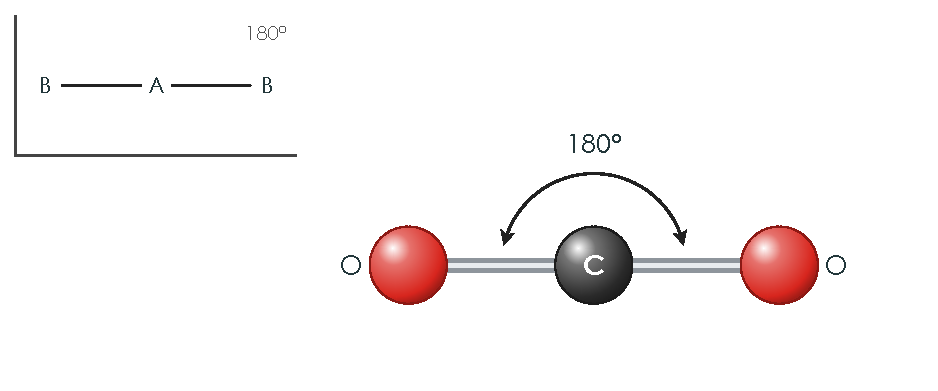
\includegraphics[width=\linewidth,height=2.8cm,keepaspectratio]{images/UD4/geo_lineal}\\ \small Lineal (\ch{CO2})\end{minipage}\hfill
    \begin{minipage}{0.32\textwidth}\centering 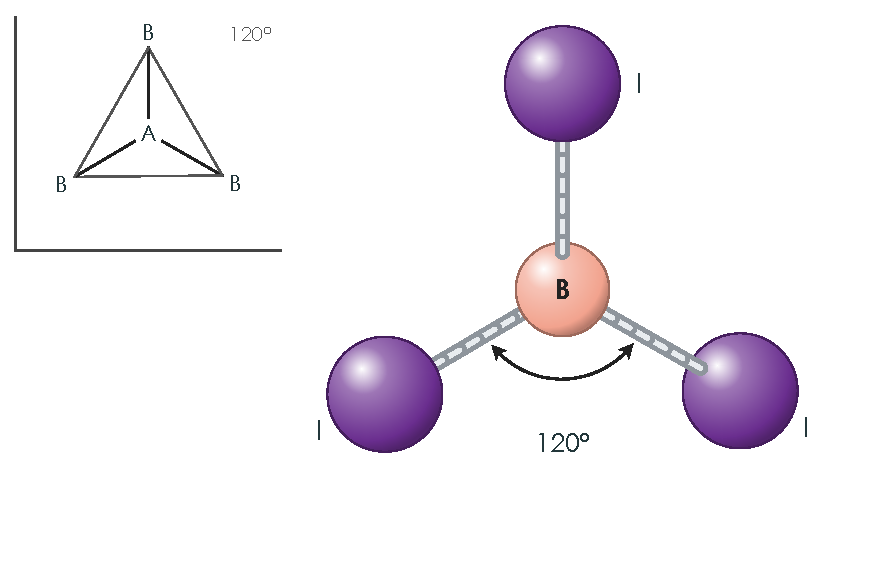
\includegraphics[width=\linewidth,height=2.8cm,keepaspectratio]{images/UD4/geo_trigonal}\\ \small Triangular plana (\ch{BI3})\end{minipage}\hfill
    \begin{minipage}{0.32\textwidth}\centering 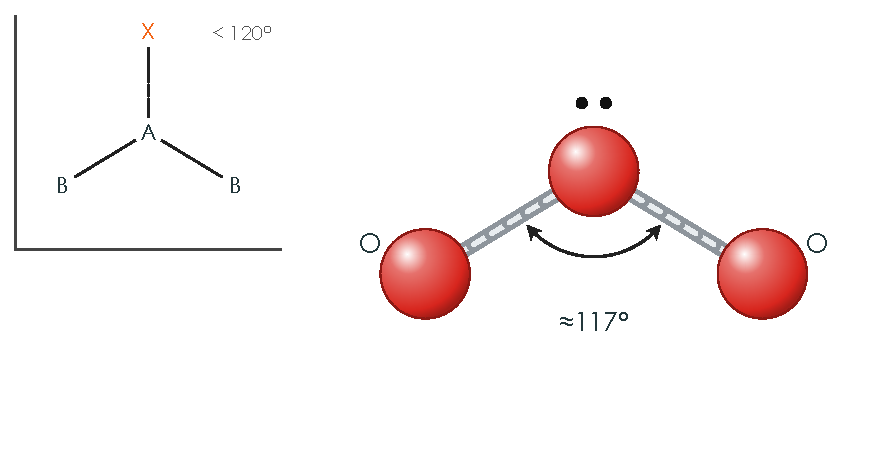
\includegraphics[width=\linewidth,height=2.8cm,keepaspectratio]{images/UD4/geo_angular3}\\ \small Angular, 1 par solitario (\ch{O3})\end{minipage}
    \\[8pt]
    \begin{minipage}{0.32\textwidth}\centering 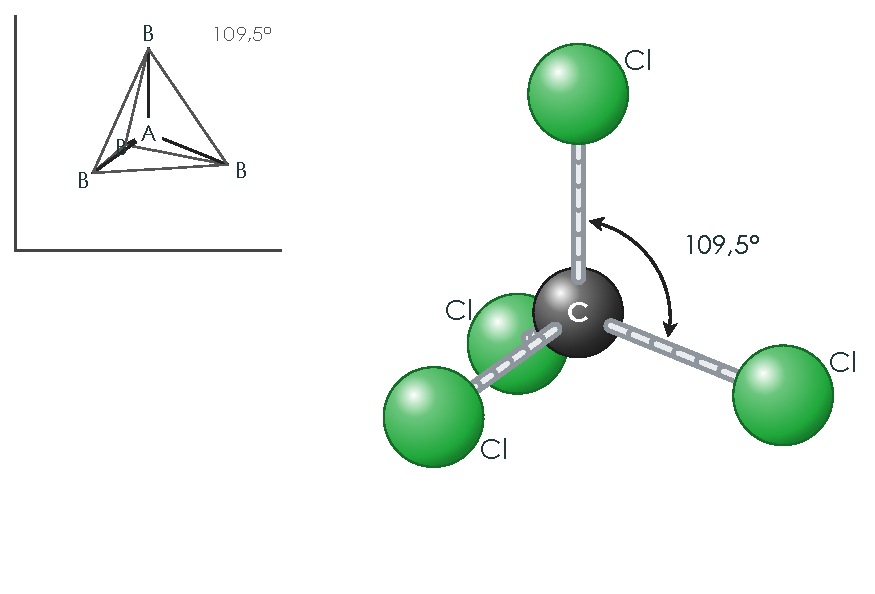
\includegraphics[width=\linewidth,height=2.8cm,keepaspectratio]{images/UD4/geo_tetraedrica}\\ \small Tetraédrica (\ch{CCl4})\end{minipage}\hfill
    \begin{minipage}{0.32\textwidth}\centering 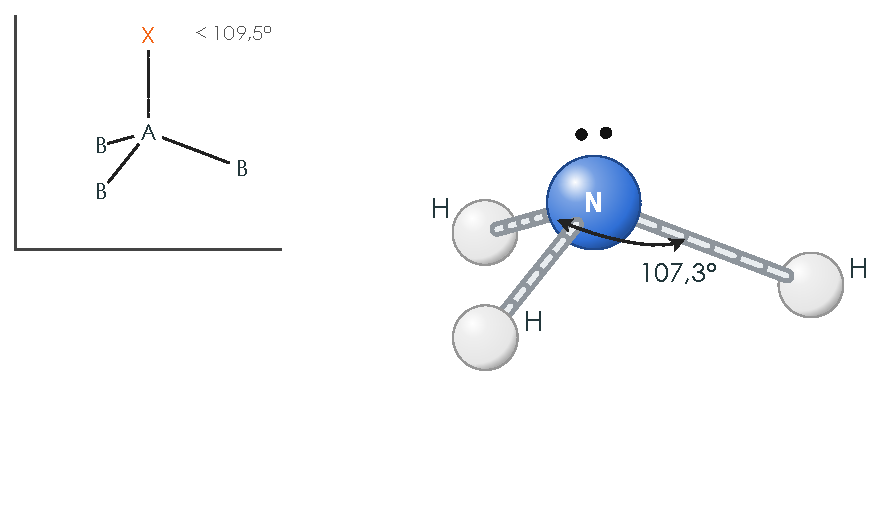
\includegraphics[width=\linewidth,height=2.8cm,keepaspectratio]{images/UD4/geo_piramidal}\\ \small Pirámide trigonal (\ch{NH3})\end{minipage}\hfill
    \begin{minipage}{0.32\textwidth}\centering 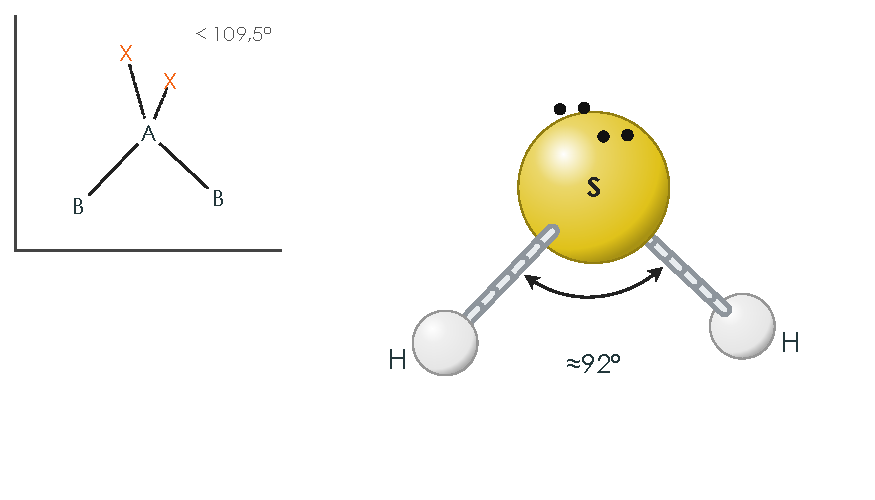
\includegraphics[width=\linewidth,height=2.8cm,keepaspectratio]{images/UD4/geo_angular4}\\ \small Angular, 2 pares solitarios (\ch{H2S})\end{minipage}
    \caption{Geometrías moleculares más sencillas. En cada una, a la izquierda, el esquema con el átomo central A, los átomos
    enlazados B y los pares solitarios X.}
    \label{fig:ud4-geometrias}
\end{figure}

\begin{example}
    \textbf{Geometría del agua.} ¿Por qué la molécula de agua es angular y no lineal?

    \textbf{Solución.} El oxígeno del agua tiene \textbf{cuatro} pares de electrones en su capa de valencia: dos enlazantes (con
    los H) y dos solitarios. Los cuatro pares se dirigen hacia los vértices de un tetraedro; como solo dos de ellos tienen átomo,
    la molécula es \textbf{angular}. Los pares solitarios repelen con más fuerza y cierran el ángulo H--O--H desde
    \ang{109.5} hasta \ang{104.5} (figura~\ref{fig:ud4-repulsiones}).
\end{example}

\begin{figure}[H]
    \centering
    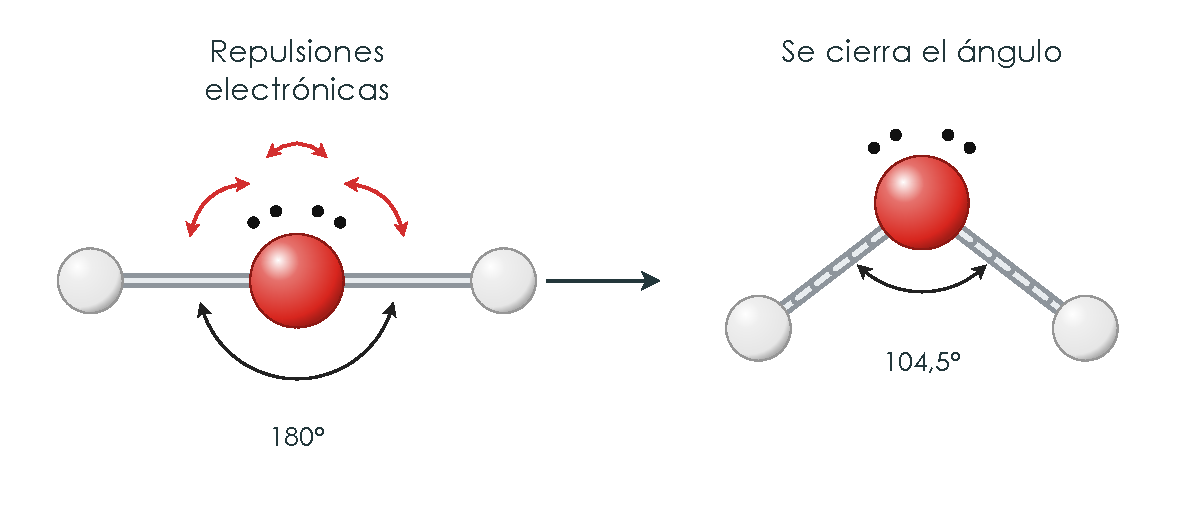
\includegraphics[width=0.55\textwidth]{images/UD4/repulsiones}
    \caption{Los pares solitarios del oxígeno repelen a los enlaces y la molécula de agua se dobla.}
    \label{fig:ud4-repulsiones}
\end{figure}

\subsection{Polaridad de las moléculas}

Una molécula es \textbf{polar} cuando tiene una zona con más densidad de carga negativa y otra con menos: se comporta como un
dipolo. Que lo sea depende de sus \textbf{enlaces} y de su \textbf{geometría}.

\begin{definition}[Momento dipolar de una molécula]
    Es la \textbf{suma vectorial} de los momentos dipolares de todos sus enlaces.
    \begin{itemize}
        \item Si todos los enlaces son apolares, la molécula es \textbf{apolar} (\ch{H2}, \ch{Cl2}).
        \item Si tiene enlaces polares, puede ser \textbf{polar} o \textbf{apolar}: si la molécula es simétrica, los momentos de los
        enlaces se anulan y es apolar (\(\vec{\mu} = 0\)); si no, es polar (\(\vec{\mu} \neq 0\)).
    \end{itemize}
\end{definition}

\begin{figure}[H]
    \centering
    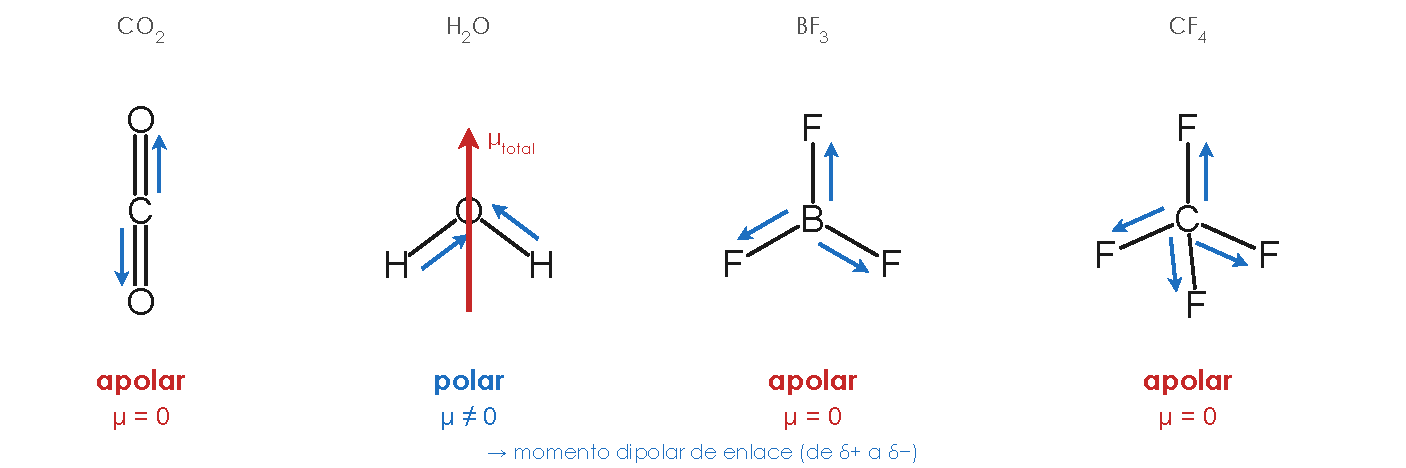
\includegraphics[width=0.75\textwidth]{images/UD4/polaridad_moleculas}
    \caption{El \ch{CO2}, el \ch{BF3} y el \ch{CF4} tienen enlaces polares pero son simétricos: sus momentos se anulan. El agua,
    angular, es polar.}
    \label{fig:ud4-polaridad}
\end{figure}

Por ejemplo, el \ch{CO2} y el \ch{CF4} tienen enlaces polares, pero por su simetría (lineal y tetraédrica) son
\textbf{apolares}; el \ch{H2O} (angular), el \ch{NH3} (piramidal) y el \ch{CH3F} (tetraédrica, pero con un átomo distinto) son
\textbf{polares} (figura~\ref{fig:ud4-polaridad}).

\begin{exercise}
    Predice la geometría y la polaridad de estas moléculas: a) \ch{BCl3}; b) \ch{PH3}; c) \ch{SiH4}; d) \ch{H2S}; e) \ch{CHCl3}.
    \begin{solu}
        a) 3 pares enlazantes: \textcolor{red}{triangular plana, apolar}. b) 3 enlazantes y 1 solitario:
        \textcolor{red}{pirámide trigonal, polar}. c) 4 enlazantes: \textcolor{red}{tetraédrica, apolar}. d) 2 enlazantes y 2
        solitarios: \textcolor{red}{angular, polar}. e) 4 enlazantes, pero un H y tres Cl: \textcolor{red}{tetraédrica
        (deformada), polar}: los momentos de los enlaces no se anulan.
    \end{solu}
\end{exercise}

\begin{exercise}
    El \ch{BF3} y el \ch{NF3} tienen fórmulas parecidas. Sin embargo, el primero es apolar y el segundo, polar. Explícalo.
    \begin{solu}
        El B tiene 3 electrones de valencia y forma 3 enlaces sin pares solitarios: \textcolor{red}{\ch{BF3} es triangular plana}
        y los tres momentos de enlace, iguales y a \ang{120}, se anulan. El N tiene 5: forma 3 enlaces y le queda un par
        solitario: \textcolor{red}{\ch{NF3} es una pirámide trigonal} y los momentos no se anulan.
    \end{solu}
\end{exercise}

\subsection{Fuerzas intermoleculares}

El \textbf{estado físico} de una sustancia depende de la intensidad de las fuerzas entre sus partículas. Que una sustancia
covalente molecular pueda ser sólida o líquida demuestra que sus \textbf{moléculas se atraen entre sí}.

\begin{remark}
    \textbf{Intra- e intermolecular.} Los enlaces covalentes unen a los átomos \textbf{dentro} de la molécula: son fuerzas
    \textbf{intra}moleculares, muy intensas. Las fuerzas \textbf{inter}moleculares actúan \textbf{entre} moléculas distintas y son
    mucho más débiles. Al hervir agua no se rompen las moléculas de \ch{H2O}: solo se separan unas de otras.
\end{remark}

Las fuerzas intermoleculares, que a veces se llaman en conjunto \textbf{fuerzas de Van der Waals}, son de tres tipos, y su
intensidad depende sobre todo de la polaridad de las moléculas:

\paragraph{Fuerzas dipolo-dipolo.} Una molécula \textbf{polar} es un dipolo permanente: la parte negativa de una molécula atrae a
la parte positiva de la vecina (figura~\ref{fig:ud4-dipolo}). Se dan, por ejemplo, entre las moléculas de \ch{HCl} o de
\ch{H2S}.

\begin{figure}[H]
    \centering
    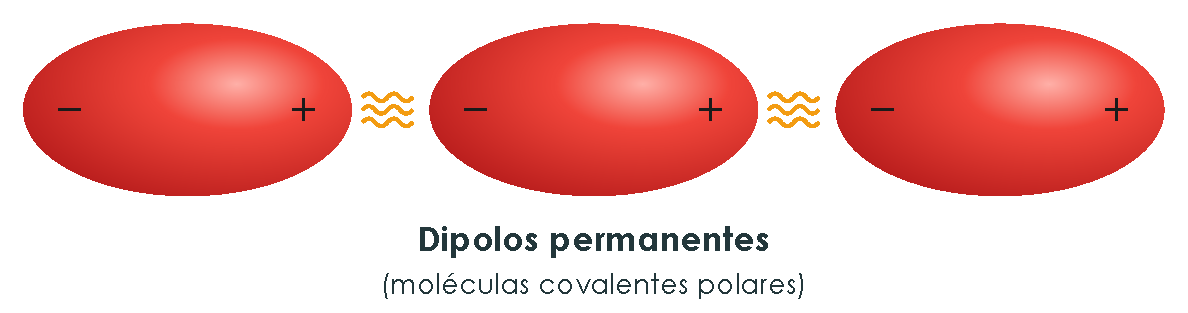
\includegraphics[width=0.6\textwidth]{images/UD4/dipolo_dipolo}
    \caption{Fuerzas dipolo-dipolo entre moléculas polares.}
    \label{fig:ud4-dipolo}
\end{figure}

\paragraph{Fuerzas de dispersión (o de London).} Incluso en las moléculas \textbf{apolares}, el movimiento continuo de los
electrones hace que, en un instante dado, haya más carga negativa en un extremo que en otro: se forma un \textbf{dipolo
instantáneo}, que a su vez deforma la nube de la molécula vecina y crea en ella un \textbf{dipolo inducido}
(figura~\ref{fig:ud4-dispersion}). Las dos se atraen durante un instante. Son fuerzas muy débiles, pero existen entre
\textbf{todas} las moléculas, y son tanto más intensas cuanto \textbf{mayor} es la molécula: tiene más electrones y su nube es
más fácil de deformar. Por eso, a temperatura ambiente, el \ch{F2} y el \ch{Cl2} son gases, el \ch{Br2} es líquido y el \ch{I2},
sólido.

\begin{figure}[H]
    \centering
    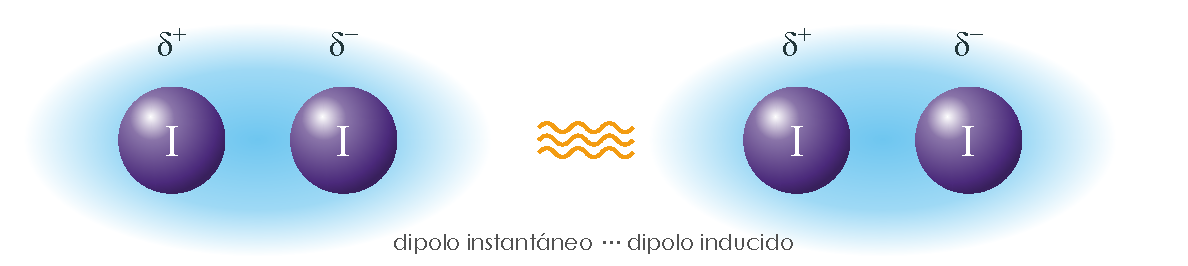
\includegraphics[width=0.6\textwidth]{images/UD4/dispersion}
    \caption{Fuerzas de dispersión: un dipolo instantáneo induce otro en la molécula vecina.}
    \label{fig:ud4-dispersion}
\end{figure}

\paragraph{Enlace (o puente) de hidrógeno.} Cuando el hidrógeno está unido a un átomo \textbf{muy electronegativo y pequeño}
(\textbf{F}, \textbf{O} o \textbf{N}), el enlace es muy polar y el H queda casi «desnudo», con una carga positiva parcial
grande. Ese H es atraído con fuerza por un par solitario del F, O o N de una molécula vecina (figura~\ref{fig:ud4-puentes}).
Es la fuerza intermolecular más intensa, aunque sigue siendo unas diez veces más débil que un enlace covalente. Se da en el
\ch{HF}, el \ch{H2O}, el \ch{NH3}, los alcoholes o el ADN, cuyas dos hebras se mantienen unidas por puentes de hidrógeno.

\begin{figure}[H]
    \centering
    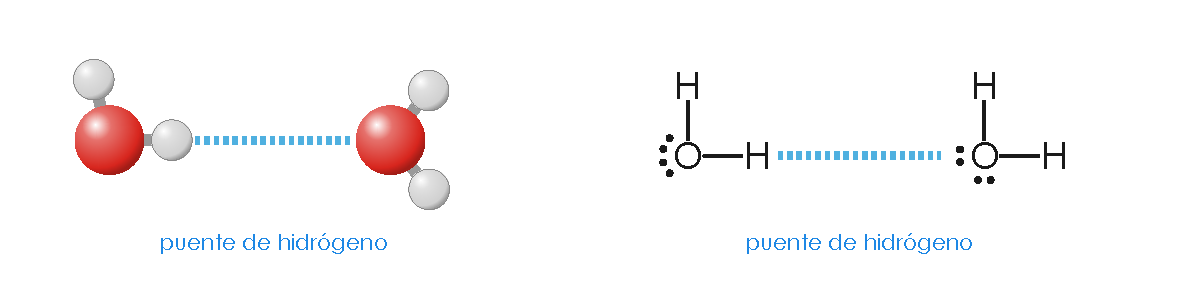
\includegraphics[width=0.6\textwidth]{images/UD4/puentes_H_agua}
    \caption{Enlace de hidrógeno entre dos moléculas de agua.}
    \label{fig:ud4-puentes}
\end{figure}

Los enlaces de hidrógeno explican por qué el agua es líquida a temperatura ambiente cuando las sustancias parecidas a ella (\ch{H2S},
\ch{H2Se}, \ch{H2Te}) son gases: si no fuera por ellos, el agua herviría a unos \qty{-80}{\degreeCelsius}
(figura~\ref{fig:ud4-hidruros}). Lo mismo les ocurre al \ch{HF} y al \ch{NH3} en sus grupos. En el grupo 14, cuyos hidruros son
apolares, el punto de ebullición sube regularmente con el tamaño de la molécula.

\begin{figure}[H]
    \centering
    \begin{tikzpicture}
        \begin{axis}[grafica, width=0.7\linewidth, height=6.2cm,
            xmin=1.7, xmax=5.3, ymin=-180, ymax=120, xtick={2,3,4,5}, xlabel={Periodo},
            ylabel={Temperatura de ebullición (\unit{\degreeCelsius})}, ytick={-150,-100,-50,0,50,100},
            legend style={font=\scriptsize, at={(1.02,0.5)}, anchor=west, draw=none}, legend cell align=left]
            \addplot[thick, mark=*, red!70!black] coordinates {(2,100) (3,-60.3) (4,-41.3) (5,-2)};
            \addplot[thick, mark=square*, ocre] coordinates {(2,19.5) (3,-85) (4,-66.8) (5,-35.4)};
            \addplot[thick, mark=triangle*, blue!70!black] coordinates {(2,-33.3) (3,-87.7) (4,-62.5) (5,-17)};
            \addplot[thick, mark=diamond*, gray] coordinates {(2,-161.5) (3,-111.9) (4,-88.5) (5,-52)};
            \legend{Grupo 16: \ch{H2O} \dots\ \ch{H2Te}, Grupo 17: \ch{HF} \dots\ \ch{HI}, Grupo 15: \ch{NH3} \dots\ \ch{SbH3},
                Grupo 14: \ch{CH4} \dots\ \ch{SnH4}}
        \end{axis}
    \end{tikzpicture}
    \caption{Temperatura de ebullición de los hidruros de los grupos 14 a 17. El \ch{H2O}, el \ch{HF} y el \ch{NH3} se salen de
    la tendencia por los enlaces de hidrógeno.}
    \label{fig:ud4-hidruros}
\end{figure}

\subsection{Propiedades de las sustancias covalentes moleculares}

\begin{itemize}
    \item A temperatura ambiente pueden ser gases (\ch{O2}, \ch{CO2}), líquidos (agua, etanol) o sólidos (yodo, azúcar), pero todas
    tienen \textbf{puntos de fusión y ebullición bajos}, porque solo hay que vencer las débiles fuerzas intermoleculares.
    \item En estado sólido son \textbf{blandas} y \textbf{frágiles}, por la misma razón.
    \item \textbf{No conducen la electricidad}: los electrones están localizados en los enlaces y no hay cargas libres.
    \item Su \textbf{solubilidad} depende de su polaridad, según la regla «lo semejante disuelve a lo semejante»: las sustancias
    \textbf{polares} se disuelven en disolventes polares, como el agua, y las \textbf{apolares}, en disolventes apolares, como la
    gasolina, el tetracloruro de carbono o el hexano.
\end{itemize}

\begin{example}
    \textbf{¿Por qué el agua es líquida y el dióxido de carbono, gas?} A temperatura ambiente, el agua (\(M = \qty{18}{\gram\per\mol}\))
    es líquida, mientras que el \ch{CO2} (\(M = \qty{44}{\gram\per\mol}\)) es un gas. Explícalo.

    \textbf{Solución.} Las dos son sustancias covalentes moleculares, así que su estado depende de las fuerzas entre sus moléculas.
    El \ch{CO2} es lineal y \textbf{apolar}: entre sus moléculas solo hay fuerzas de dispersión, débiles. El agua es angular y muy
    \textbf{polar}, y sus moléculas, con H unidos a O, forman \textbf{enlaces de hidrógeno}, mucho más intensos. Aunque la
    molécula de \ch{CO2} es mayor, separar las moléculas de agua cuesta mucha más energía: el agua hierve a
    \qty{100}{\degreeCelsius} y el \ch{CO2} sublima a \qty{-78}{\degreeCelsius}.
\end{example}

\begin{exercise}
    ¿Cuáles de estas sustancias serán solubles en agua? a) \ch{CH3OH} (metanol); b) \ch{N2}; c) \ch{KBr}; d) \ch{C8H18} (octano);
    e) \ch{NH3}; f) \ch{Cl2}; g) sacarosa, \ch{C12H22O11}.
    \begin{solu}
        Solubles: \textcolor{red}{a) metanol, c) \ch{KBr}, e) \ch{NH3} y g) sacarosa}: el \ch{KBr} es iónico, y el metanol, el
        amoníaco y la sacarosa son polares y forman enlaces de hidrógeno con el agua. \textcolor{red}{Poco o nada solubles: b),
        d) y f)}, que son apolares.
    \end{solu}
\end{exercise}

\begin{exercise}
    ¿Qué fuerzas intermoleculares hay entre las moléculas de cada una de estas sustancias? a) \ch{CH4}; b) \ch{HBr}; c) \ch{NH3};
    d) \ch{I2}; e) \ch{CH3CH2OH} (etanol).
    \begin{solu}
        a) \textcolor{red}{Solo de dispersión} (apolar). b) \textcolor{red}{Dipolo-dipolo y de dispersión}. c) \textcolor{red}{Enlaces
        de hidrógeno} (H unido a N), además de dipolo-dipolo y dispersión. d) \textcolor{red}{De dispersión}; como la molécula es
        grande, son bastante intensas y el yodo es sólido. e) \textcolor{red}{Enlaces de hidrógeno} (grupo O--H), dipolo-dipolo y
        dispersión.
    \end{solu}
\end{exercise}

\begin{exercise}
    Ordena de menor a mayor punto de ebullición: \ch{Cl2}, \ch{F2}, \ch{I2} y \ch{Br2}. ¿Qué fuerzas intermoleculares lo explican?
    \begin{solu}
        Son moléculas apolares y entre ellas solo hay \textcolor{red}{fuerzas de dispersión}, que aumentan con el tamaño (el número
        de electrones) de la molécula: \textcolor{red}{\(\ch{F2} < \ch{Cl2} < \ch{Br2} < \ch{I2}\)} (\(-188\), \(-34\), 59 y
        \qty{184}{\degreeCelsius}).
    \end{solu}
\end{exercise}

%========================================================================================
\section{Cristales covalentes}\label{sec:ud4-cristales}
%========================================================================================

En algunas sustancias, como el \textbf{diamante} y el \textbf{grafito} (dos formas del carbono) o la \textbf{sílice} (\ch{SiO2},
el cuarzo), los átomos se unen por enlaces covalentes formando \textbf{redes gigantes} en lugar de moléculas. Los átomos se
ordenan geométricamente en el espacio, así que estas sustancias tienen estructura \textbf{cristalina}: son \textbf{cristales
covalentes} (o sólidos covalentes).

\begin{itemize}
    \item En el \textbf{diamante}, cada átomo de carbono está unido a otros \textbf{cuatro} por enlaces covalentes, dirigidos
    hacia los vértices de un tetraedro, y la red se extiende en las tres direcciones (figura~\ref{fig:ud4-carbono}).
    \item En el \textbf{grafito}, cada carbono se une a otros \textbf{tres}, y forman \textbf{láminas} planas de hexágonos. Las
    láminas se apilan unas sobre otras unidas solo por fuerzas de dispersión, débiles, y el cuarto electrón de cada carbono queda
    deslocalizado por la lámina. Una sola lámina de grafito es el \textbf{grafeno}.
    \item En el \textbf{cuarzo}, cada átomo de silicio está unido a cuatro de oxígeno, y cada oxígeno a dos de silicio.
\end{itemize}

\begin{figure}[H]
    \centering
    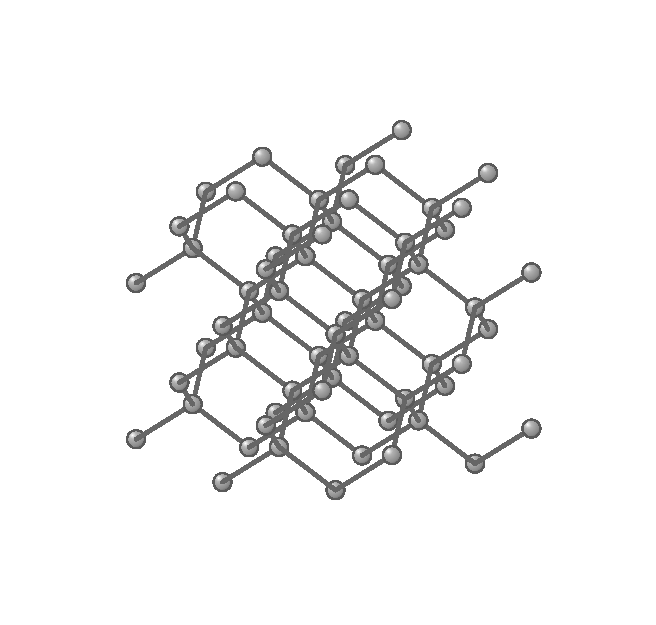
\includegraphics[width=0.4\textwidth]{images/UD4/diamante}\hspace{1cm}
    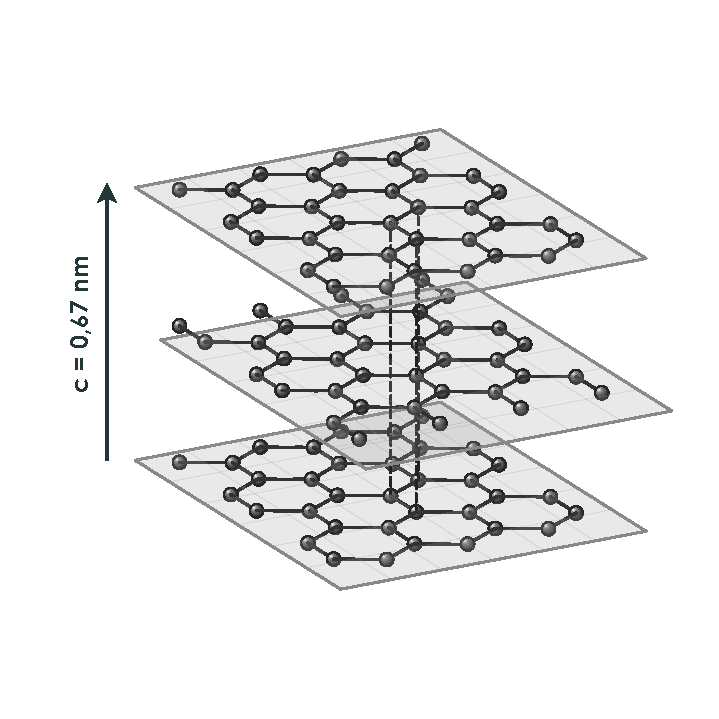
\includegraphics[width=0.4\textwidth]{images/UD4/grafito}
    \caption{Estructura del diamante (izquierda) y del grafito (derecha), con sus láminas separadas \qty{0.335}{\nm}.}
    \label{fig:ud4-carbono}
\end{figure}

\paragraph{Propiedades de los cristales covalentes.} Se deben a que el enlace covalente es el más fuerte de todos y a que, para
fundir o rayar el cristal, hay que romper un número enorme de enlaces:
\begin{itemize}
    \item Son \textbf{sólidos} con \textbf{puntos de fusión altísimos}, de miles de grados (el diamante se transforma a unos
    \qty{3550}{\degreeCelsius}; el cuarzo funde a \qty{1713}{\degreeCelsius}).
    \item Son \textbf{muy duros}: el diamante, con un 10 en la escala de Mohs, es la sustancia natural más dura.
    \item Sin embargo, son \textbf{frágiles}: los enlaces tienen direcciones fijas y se rompen si un golpe deforma la red.
    \item \textbf{No conducen la electricidad}, porque los electrones están localizados en los enlaces. La excepción es el
    \textbf{grafito}, que conduce a lo largo de sus láminas gracias a los electrones deslocalizados.
    \item Son \textbf{insolubles} en todos los disolventes.
\end{itemize}

\begin{remark}
    \textbf{El cristal de las ventanas no es un cristal.} El vidrio está hecho, sobre todo, de sílice, como el cuarzo, pero sus
    átomos están colocados de forma \textbf{desordenada}: no tiene estructura cristalina, sino \textbf{amorfa}. Por eso no funde a una
    temperatura fija, sino que se va reblandeciendo poco a poco, lo que permite soplarlo y moldearlo.
\end{remark}

\begin{example}
    \textbf{Diamante y grafito.} Si el diamante y el grafito están formados solo por átomos de carbono, ¿por qué el diamante es la
    sustancia natural más dura y el grafito es tan blando que se usa en las minas de los lápices?

    \textbf{Solución.} La diferencia está en cómo se unen los átomos. En el diamante, cada carbono forma cuatro enlaces covalentes
    con otros cuatro, en una red tridimensional: para rayarlo hay que romper enlaces covalentes en todas las direcciones. En el
    grafito, los átomos forman láminas unidas entre sí solo por fuerzas de dispersión: las láminas se deslizan unas sobre otras con
    facilidad y se quedan pegadas en el papel al escribir.
\end{example}

\begin{exercise}
    Busca información sobre otro cristal covalente (el carburo de silicio, el nitruro de boro o el propio cuarzo): su estructura,
    sus propiedades y sus usos. Compáralo con el diamante.
    \begin{solu}
        \textcolor{red}{Respuesta abierta.} Por ejemplo, el \textcolor{red}{carburo de silicio, \ch{SiC}} (carborundo), tiene una
        estructura como la del diamante con átomos de Si y C alternados; tiene una dureza de 9,5, funde a unos
        \qty{2700}{\degreeCelsius} y se usa en lijas, discos de corte, frenos cerámicos y en electrónica de potencia (es
        semiconductor). Es algo menos duro que el diamante pero más barato y resistente a la oxidación.
    \end{solu}
\end{exercise}

\begin{exercise}
    ¿Por qué el grafito conduce la electricidad y el diamante no? ¿En qué dirección conduce mejor el grafito?
    \begin{solu}
        \textcolor{red}{En el grafito, cada carbono usa solo tres electrones en enlaces y el cuarto queda deslocalizado por la
        lámina}; en el diamante los cuatro están localizados en enlaces. El grafito conduce mucho mejor
        \textcolor{red}{en la dirección de las láminas} que perpendicularmente a ellas.
    \end{solu}
\end{exercise}

%========================================================================================
\section{Propiedades de las sustancias}\label{sec:ud4-propiedades}
%========================================================================================

Según el tipo de enlace y las partículas que las forman, las sustancias se pueden clasificar en cuatro grupos
(figura~\ref{fig:ud4-tipos-sustancias}), con propiedades muy diferentes (tabla~\ref{tab:ud4-propiedades}).

\begin{figure}[H]
    \centering
    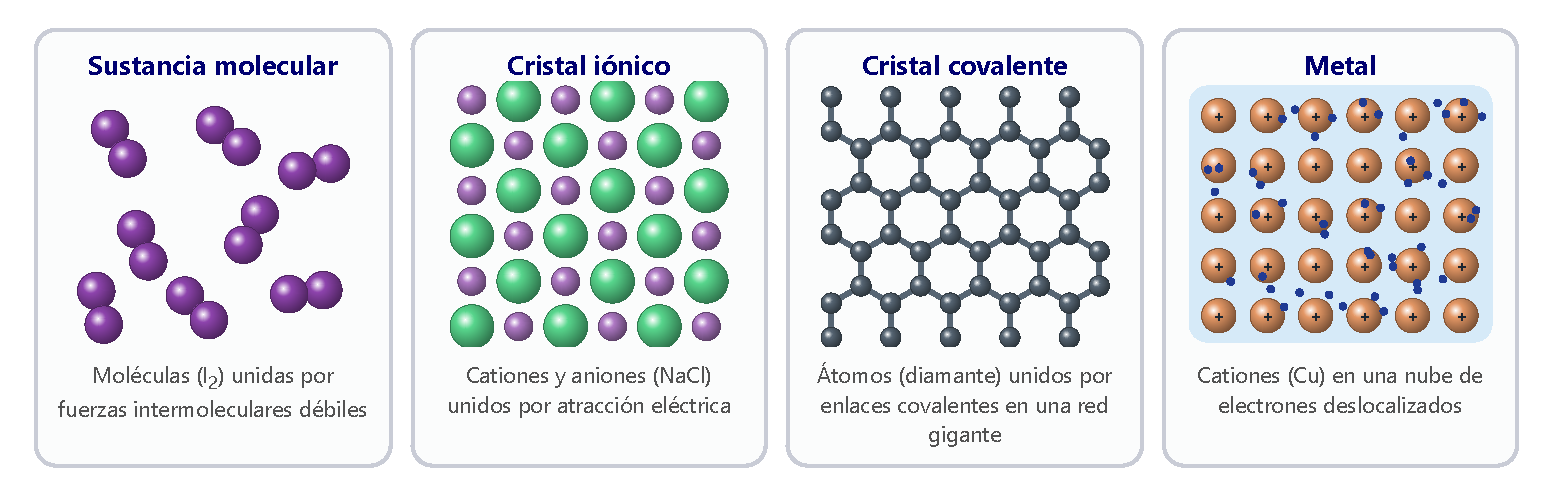
\includegraphics[width=\textwidth]{images/UD4/tipos_sustancias}
    \caption{Las cuatro clases de sustancias según su enlace.}
    \label{fig:ud4-tipos-sustancias}
\end{figure}

\begin{table}[H]
    \centering
    \caption{Propiedades de las sustancias según su tipo de enlace}
    \vspace{-5pt}
    \small
    \begin{tabular}{@{}L{2.25cm}L{2.7cm}L{2.7cm}L{2.7cm}L{2.7cm}@{}}
        \toprule
        & \textbf{Molecular} & \textbf{Metálica} & \textbf{Iónica} & \textbf{Cristal covalente} \\
        \midrule
        \textbf{Partículas} & Moléculas unidas por fuerzas intermoleculares & Cationes en una nube de electrones & Cationes y
        aniones & Átomos \\[3pt]
        \textbf{Fusión y ebullición} & Bajas & Variables (casi todos sólidos) & Altas & Muy altas \\[3pt]
        \textbf{Conductividad} & No conducen & Conducen muy bien & Solo fundidos o disueltos & No conducen (salvo el grafito) \\[3pt]
        \textbf{Dureza} & Blandas y frágiles & Tenaces, dúctiles y maleables & Duros pero frágiles & Muy duros pero frágiles \\[3pt]
        \textbf{Solubilidad} & Polares en polares; apolares en apolares & Insolubles (forman aleaciones) & Solubles en disolventes
        polares & Insolubles \\
        \bottomrule
    \end{tabular}
    \label{tab:ud4-propiedades}
\end{table}

\begin{example}
    \textbf{Identificar el enlace por las propiedades.} Una sustancia blanca funde a \qty{1074}{\degreeCelsius}, se disuelve en
    agua y su disolución conduce la electricidad, pero el sólido no. Otra, también blanca, funde a \qty{186}{\degreeCelsius}, se
    disuelve en agua y su disolución no conduce. ¿Qué tipo de sustancia es cada una?

    \textbf{Solución.} La primera tiene un punto de fusión alto y conduce solo disuelta, cuando sus iones quedan libres: es un
    \textbf{compuesto iónico} (puede ser el \ch{KCl}, que funde a \qty{770}{\degreeCelsius}, o el \ch{NaF}). La segunda funde a
    baja temperatura y no da iones en disolución: es una \textbf{sustancia covalente molecular} y, como se disuelve en agua,
    \textbf{polar} (puede ser la glucosa).
\end{example}

\subsection{Materiales de interés estratégico}

Un teléfono móvil contiene unos 40 elementos químicos distintos. Algunos materiales, como el \textbf{grafito}, el
\textbf{cobalto}, el \textbf{litio} o las \textbf{tierras raras}, se han vuelto imprescindibles para fabricar baterías, chips,
pantallas, imanes de motores eléctricos, aerogeneradores o placas solares, y su demanda no deja de crecer. Se consideran
\textbf{materiales de interés estratégico}, porque de ellos dependen sectores clave como la movilidad eléctrica, la producción de
energía o la defensa de un país.

El problema es que sus yacimientos están concentrados en muy pocos lugares, y su suministro se ve afectado por guerras,
conflictos comerciales o crisis como la de la pandemia de COVID-19. Un ejemplo es el \textbf{coltán}, una mezcla de los minerales
columbita y tantalita de la que se extrae el tántalo, con el que se fabrican condensadores diminutos. Gran parte procede de la
República Democrática del Congo, donde su extracción ha financiado conflictos armados y se hace a menudo en condiciones
durísimas.

Las soluciones pasan por \textbf{investigar} nuevos materiales, más abundantes, que sustituyan a los escasos, y por la
\textbf{economía circular}: alargar la vida de los aparatos, repararlos, reutilizarlos y, al final, reciclarlos para recuperar
sus materiales.

\begin{exercise}
    Para las sustancias \ch{LiBr}, \ch{Ag}, \ch{N2} y \ch{SiO2}: a) indica el tipo de enlace de cada una; b) ¿cuáles conducen la
    electricidad y en qué condiciones?; c) ¿cuáles son solubles en agua?
    \begin{solu}
        a) \ch{LiBr}: \textcolor{red}{iónico}; \ch{Ag}: \textcolor{red}{metálico}; \ch{N2}: \textcolor{red}{covalente molecular};
        \ch{SiO2}: \textcolor{red}{cristal covalente}. b) \textcolor{red}{La plata, siempre (sólida o fundida); el \ch{LiBr},
        fundido o disuelto}. El \ch{N2} y el \ch{SiO2} no conducen. c) \textcolor{red}{Solo el \ch{LiBr}}; el \ch{N2} es apolar y
        apenas se disuelve, y la plata y el \ch{SiO2} son insolubles.
    \end{solu}
\end{exercise}

\begin{exercise}
    ¿Con qué tipo o tipos de enlace o de sustancia relacionas cada una de estas características? a) Se forma entre átomos
    iguales. b) Son dúctiles y maleables. c) Son duras y frágiles. d) Se disuelven en agua, pero no en hexano. e) Solo conducen la
    electricidad fundidas o disueltas. f) Se forma entre átomos de elementos distintos. g) Son buenas conductoras del calor.
    h) Forman moléculas. i) No conducen en estado sólido. j) Se debe a la atracción entre cationes y aniones.
    \begin{solu}
        a) \textcolor{red}{Covalente (\ch{H2}, diamante) y metálico}. b) \textcolor{red}{Metálicas}. c) \textcolor{red}{Iónicas y
        cristales covalentes}. d) \textcolor{red}{Iónicas y moleculares polares}. e) \textcolor{red}{Iónicas}. f)
        \textcolor{red}{Iónico y covalente (\ch{H2O}, \ch{SiO2})}. g) \textcolor{red}{Metálicas}. h) \textcolor{red}{Covalente
        (sustancias moleculares)}. i) \textcolor{red}{Iónicas, moleculares y cristales covalentes} (salvo el grafito).
        j) \textcolor{red}{Iónico}.
    \end{solu}
\end{exercise}

\begin{exercise}
    Investiga qué son las tierras raras: qué elementos son, para qué sirven y dónde se extraen. ¿Se pueden considerar
    materiales de interés estratégico?
    \begin{solu}
        \textcolor{red}{Respuesta abierta.} \textcolor{blue}{Son 17 elementos: los 15 lantánidos, el escandio y el itrio. A pesar
        del nombre, no son tan escasos en la corteza, pero están muy dispersos y su separación es difícil y contaminante. Se usan en
        imanes permanentes (neodimio) de motores eléctricos y aerogeneradores, en pantallas y ledes (europio, terbio), en láseres,
        catalizadores y baterías. La mayor parte se extrae y refina en China.} \textcolor{red}{Sí son estratégicas}: son
        imprescindibles para la transición energética y su suministro depende de muy pocos países.
    \end{solu}
\end{exercise}

%========================================================================================
\section{Química en la vida: pegarse como un gecko}\label{sec:ud4-gecko}
%========================================================================================

Durante siglos nadie supo cómo los geckos se pegaban a las paredes. Se pensó en ventosas, en un pegamento o en ganchos
microscópicos, pero ninguna explicación funcionaba: los geckos se adhieren también al vidrio pulido y en el vacío, y sus pies no
dejan ningún residuo. En el año 2000, un equipo de biólogos e ingenieros de California consiguió medir la fuerza de uno solo de
los pelillos de sus dedos, las \textbf{sétulas}, y en 2002 demostró que se trataba de \textbf{fuerzas de Van der Waals}, en
concreto de fuerzas de dispersión: funcionaban igual sobre superficies polares y apolares.

Cada dedo de un gecko tiene cientos de miles de sétulas, de unas 100 micras de largo, que se ramifican en cientos de puntas de
unos \qty{200}{\nm}. Como las fuerzas de dispersión solo actúan a distancias pequeñísimas, cuantas más puntas toquen la
superficie, más fuerza hay. Un gecko de unos \qty{70}{\gram} podría, en teoría, sostener más de cien kilos. Para despegarse no
tiene que hacer fuerza: le basta con doblar el dedo y separar las puntas poco a poco, como quien despega una tira de celo.

Inspirándose en los geckos (es lo que se llama \textbf{biomímesis}), se están desarrollando adhesivos secos que no se ensucian ni
dejan restos y se pueden despegar y pegar miles de veces, guantes para escalar paredes lisas, pinzas para robots que manipulan
objetos delicados y robots trepadores capaces de moverse por el exterior de una nave espacial para repararla.

\begin{exercise}
    a) ¿Por qué decimos que el gecko se pega gracias a fuerzas intermoleculares y no gracias a enlaces químicos? b) ¿Por qué
    necesita tantísimos pelillos? c) Investiga otro ejemplo de biomímesis (el velcro, la hoja de loto, la piel de tiburón…) y
    explica en qué se inspira.
    \begin{solu}
        a) \textcolor{red}{Porque no se forman enlaces entre las moléculas de la pata y las de la pared}: solo hay atracciones
        débiles entre dipolos instantáneos e inducidos, que se rompen sin esfuerzo y no dejan residuos. b) \textcolor{red}{Las
        fuerzas de dispersión son muy débiles y solo actúan a distancias de pocos nanómetros}: cada punta aporta muy poco, y hace
        falta que millones de ellas estén en contacto íntimo con la superficie. c) \textcolor{red}{Respuesta abierta.} Por
        ejemplo, el velcro imita los ganchitos de los frutos del cardo; las pinturas autolimpiables, la superficie de la hoja de
        loto, que repele el agua, y algunos bañadores, la piel del tiburón.
    \end{solu}
\end{exercise}

%========================================================================================
\section{Prácticas}\label{sec:ud4-practicas}
%========================================================================================

\subsection{¿Qué enlace tiene? Clasificar sustancias por sus propiedades}

\noindent\begin{minipage}[t]{0.48\textwidth}
    \textbf{Objetivo}
    \begin{itemize}
        \item Clasificar varias sustancias según su tipo de enlace a partir de su solubilidad, su conductividad eléctrica y su
        facilidad para fundirse.
    \end{itemize}
\end{minipage}\hfill
\begin{minipage}[t]{0.48\textwidth}
    \textbf{Material y reactivos}
    \begin{itemize}
        \item Pila de \qty{9}{\volt}, un led (o una bombilla pequeña), cables con pinzas, dos electrodos de grafito o de cobre,
        vasos de precipitados, tubos de ensayo, mechero y cucharilla metálica.
        \item Agua destilada, aceite o hexano, sal común, azúcar, parafina (o una vela), arena fina, una lámina de cobre o un
        clavo y la mina de un lápiz.
    \end{itemize}
\end{minipage}

\textbf{Procedimiento}
\begin{enumerate}[label=\numberballgreen]
    \item Monta un circuito con la pila, el led y los dos electrodos separados. Comprueba que el led se enciende al juntar los
    electrodos.
    \item \textbf{Conductividad en sólido}: toca con los electrodos la lámina de cobre, la mina de lápiz, un montoncito de sal,
    de azúcar, de parafina y de arena. Anota si el led se enciende.
    \item \textbf{Solubilidad}: pon una punta de espátula de cada sólido en un tubo con agua destilada y en otro con aceite o
    hexano. Agita y anota si se disuelve.
    \item \textbf{Conductividad en disolución}: introduce los electrodos en el agua destilada sola y después en cada disolución
    acuosa. Anota el resultado.
    \item \textbf{Punto de fusión}: calienta con cuidado una pequeña cantidad de cada sólido en la cucharilla y anota si funde
    fácilmente o no.
\end{enumerate}
\textbf{Trabaja con gafas y bata. El hexano es inflamable: mantenlo lejos de la llama. No calientes el aceite.}

\begin{exercise}
    a) Recoge los resultados en una tabla y clasifica cada sustancia como iónica, metálica, covalente molecular o cristal
    covalente. b) ¿Por qué hay que comprobar antes que el agua destilada no conduce? c) ¿Qué sustancia te ha parecido más difícil
    de clasificar? ¿Por qué?
    \begin{solu}
        a) \textcolor{red}{Iónica: la sal} (no conduce sólida, sí disuelta; soluble en agua; no funde en la cucharilla).
        \textcolor{red}{Metálica: el cobre} (conduce en sólido). \textcolor{red}{Moleculares: el azúcar} (polar: soluble en agua,
        su disolución no conduce, funde y se carameliza con facilidad) \textcolor{red}{y la parafina} (apolar: soluble en hexano,
        funde enseguida). \textcolor{red}{Cristal covalente: la arena} (\ch{SiO2}: insoluble, no conduce, no funde) \textcolor{red}{y
        el grafito de la mina}, que conduce aunque no es un metal. b) \textcolor{red}{Para asegurarnos de que la corriente se debe a
        los iones del soluto} y no a impurezas del agua. c) \textcolor{red}{Respuesta abierta}; suele ser el grafito, que conduce
        como un metal pero es un cristal covalente.
    \end{solu}
\end{exercise}

\subsection{Química en la cocina: un chorro de agua que se dobla}

\noindent\begin{minipage}[t]{0.48\textwidth}
    \textbf{Objetivo}
    \begin{itemize}
        \item Comprobar que las moléculas de agua son polares y compararlas con las de un líquido apolar.
    \end{itemize}
\end{minipage}\hfill
\begin{minipage}[t]{0.48\textwidth}
    \textbf{Material}
    \begin{itemize}
        \item Un grifo, un peine de plástico o un globo, un jersey de lana (o el pelo seco), una bureta o una botella de plástico con
        un agujerito en el tapón, aceite de girasol y un vaso.
    \end{itemize}
\end{minipage}

\textbf{Procedimiento}
\begin{enumerate}[label=\numberballgreen]
    \item Abre el grifo de forma que salga un chorro muy fino y continuo.
    \item Frota con fuerza el peine o el globo con la lana o con el pelo, para cargarlo eléctricamente.
    \item Acerca el peine al chorro de agua, sin tocarlo, y observa qué ocurre.
    \item Repite la experiencia con un chorro fino de aceite que caiga de la botella al vaso.
\end{enumerate}
\textbf{Truco}: la experiencia sale mejor los días secos; si hay mucha humedad, el peine se descarga enseguida.

\begin{exercise}
    a) ¿Qué le ocurre al chorro de agua al acercarle el peine? ¿Y al de aceite? b) Explícalo a partir de la polaridad de las
    moléculas. c) ¿Se curvaría el chorro de agua hacia el peine tanto si este tiene carga positiva como negativa? ¿Por qué?
    \begin{solu}
        a) \textcolor{red}{El chorro de agua se curva claramente hacia el peine; el de aceite apenas se desvía.}
        b) \textcolor{red}{Las moléculas de agua son dipolos}: se orientan con el extremo de carga opuesta hacia el peine y son
        atraídas. \textcolor{red}{Las del aceite son prácticamente apolares} y casi no notan la carga. c) \textcolor{red}{Sí}: si el
        peine es negativo, las moléculas le acercan su extremo positivo (los H), y si es positivo, su extremo negativo (el O); en
        los dos casos la atracción gana a la repulsión, porque el extremo más cercano está más cerca.
    \end{solu}
\end{exercise}

%========================================================================================
\section{Situación de aprendizaje: del lápiz a la batería (ODS 12)}\label{sec:ud4-ods}
%========================================================================================

El grafito es, junto con el diamante, una de las formas del carbono. Es gris oscuro, con brillo metálico, y se exfolia con mucha
facilidad: por eso es el componente principal de las minas de los lápices, de los que se fabrican millones cada día. Pero el
grafito es también un material estratégico: forma el ánodo de casi todas las baterías de iones de litio de móviles y coches
eléctricos. El \textbf{Objetivo de Desarrollo Sostenible 12} (producción y consumo responsables) nos pide usar los recursos de
forma eficiente y reducir los residuos, algo especialmente importante con los materiales escasos.

\begin{marker}
    \textbf{Reto:} elaborad un ensayo, una presentación o un vídeo sobre el grafito, desde su uso en los lápices hasta su papel en
    las baterías, y sobre lo que podemos hacer para consumir de forma más responsable los aparatos que lo contienen.
\end{marker}

\begin{enumerate}[label=\numberballred]
    \item \textbf{Investigad} el grafito: su descubrimiento, su estructura y sus propiedades; los primeros usos para escribir y la
    historia del lápiz hasta hoy. ¿Qué significan las letras H, B, HB y F de los lápices, y para qué técnicas artísticas se usa
    cada uno?
    \item \textbf{Investigad} los pigmentos de los lápices de colores: su origen, los primeros pigmentos que usó la humanidad y
    los usos de los lápices de colores en el arte (con algún artista contemporáneo).
    \item \textbf{Calculad.} a) La distancia entre las láminas del grafito es de \qty{0.335}{\nm}. Si el trazo de un lápiz deja
    una capa de grafito de \qty{0.5}{\micro\m} de espesor, ¿cuántas láminas hay en ella? b) Una batería de coche eléctrico lleva
    unos \qty{50}{\kilo\gram} de grafito. ¿Cuántos moles de carbono son? ¿Para cuántos lápices daría, si cada mina tiene
    \qty{0.8}{\gram} de grafito?
    \item \textbf{Comunicad.} Vuestro producto final debe incluir: el descubrimiento del grafito y sus características; la
    historia del lápiz; los pigmentos de los lápices de colores; los principales países productores de grafito y su impacto
    ambiental, y alguna propuesta concreta de economía circular para los aparatos electrónicos.
\end{enumerate}

\begin{exercise}
    Resuelve los cálculos del apartado 3 de la situación de aprendizaje.
    \begin{solu}
        a) \(\dfrac{\qty{0.5e-6}{\m}}{\qty{0.335e-9}{\m}} \approx \textcolor{red}{\num{1500} \text{ láminas}}\).
        b) \(n = \dfrac{\qty{50000}{\gram}}{\qty{12.0}{\gram\per\mol}} = \textcolor{red}{\qty{4.2e3}{\mol}}\) de carbono;
        \(\dfrac{\num{50000}}{\num{0.8}} = \textcolor{red}{\num{62500} \text{ lápices}}\).
    \end{solu}
\end{exercise}

    \newpage
    %! Unidad 4 — El enlace químico: ejercicios resueltos y ejercicios finales
%! Fuente: Fuentes/Quimica/Unidad 4 («Ejercicios resueltos», «Practica y calcula», «Piensa y resuelve»).
%! Enunciados adaptados con sustancias y datos cambiados; soluciones rehechas. Dificultad: \(\star\) baja, \(\star\star\) media, \(\star\star\star\) alta.
%! Electronegatividades de Pauling de la tabla tab:ud3-en (salvo donde el enunciado da otras).

\section{Ejercicios resueltos}\label{sec:ud4-resueltos}

Salvo que se indique otra cosa, usa las electronegatividades de la tabla~\ref{tab:ud3-en} y el criterio de la
tabla~\ref{tab:ud4-den}.

\begin{example}
    \textbf{Lewis, geometría y polaridad.} Determina la estructura de Lewis y la geometría del \ch{PCl3}, el \ch{CS2} y el
    \ch{CH2Cl2}. Usa la configuración electrónica de cada elemento para hallar su valencia covalente. ¿Cuáles son polares?

    \textbf{Solución.} \textbf{1. Datos}: P: \conf{[Ne]\,3s^2\,3p^3} (5 electrones de valencia, covalencia 3); Cl:
    \conf{[Ne]\,3s^2\,3p^5} (7, covalencia 1); C: \conf{[He]\,2s^2\,2p^2} (4, covalencia 4); S: \conf{[Ne]\,3s^2\,3p^4} (6,
    covalencia 2); H: \conf{1s^1} (1, covalencia 1).

    \textbf{2. \ch{PCl3}}: \(D = 5 + 3 \cdot 7 = 26\); \(N = 4 \cdot 8 = 32\); \(C = 6\): \textbf{3 enlaces}. Quedan
    \(26 - 6 = 20\) electrones: tres pares en cada Cl y \textbf{un par solitario en el P}. Con tres pares enlazantes y uno
    solitario, la molécula es una \textbf{pirámide trigonal}; los momentos de los enlaces P--Cl (\(\Delta\mathrm{EN} = 1{,}0\)) no
    se anulan: es \textbf{polar}.
    \[ \chemfig{\charge{90=\:,180=\:,270=\:}{Cl}-\charge{90=\:}{P}(-[6]\charge{0=\:,180=\:,270=\:}{Cl})-\charge{0=\:,90=\:,270=\:}{Cl}} \]

    \textbf{3. \ch{CS2}}: \(D = 4 + 2 \cdot 6 = 16\); \(N = 24\); \(C = 8\): \textbf{4 enlaces}, dos dobles. Quedan 8 electrones,
    dos pares en cada S. Sin pares solitarios en el C, la molécula es \textbf{lineal} y \textbf{apolar} (además,
    \(\Delta\mathrm{EN} = 0\)).
    \[ \chemfig{\charge{90=\:,270=\:}{S}=C=\charge{90=\:,270=\:}{S}} \]

    \textbf{4. \ch{CH2Cl2}}: \(D = 4 + 2 + 14 = 20\); \(N = 8 + 2 \cdot 2 + 2 \cdot 8 = 28\); \(C = 8\): \textbf{4 enlaces}
    simples. Quedan 12 electrones, tres pares en cada Cl. La molécula es \textbf{tetraédrica}, pero los enlaces C--H y C--Cl son
    distintos y sus momentos no se anulan: es \textbf{polar}.
    \[ \chemfig{C(-[2]H)(-[6]H)(-[4]\charge{90=\:,180=\:,270=\:}{Cl})-\charge{0=\:,90=\:,270=\:}{Cl}} \]
\end{example}

\begin{example}
    \textbf{Energía reticular.} Calcula la energía reticular del bromuro de sodio sabiendo que en su formación a partir de sus
    elementos se desprenden \qty{361}{\kilo\joule\per\mol}, y que (en \unit{\kilo\joule\per\mol}): sublimación del Na, \(+108\);
    vaporización y disociación de medio mol de \ch{Br2(l)}, \(+112\); energía de ionización del Na, \(+496\); afinidad electrónica
    del Br, \(-325\). ¿Es mayor o menor que la del \ch{NaCl} (\(\qty{-787}{\kilo\joule\per\mol}\))? ¿Por qué?

    \textbf{Solución.} \textbf{1. Planteamiento}: según el ciclo de Born-Haber, la energía del proceso global es la suma de las de
    todas las etapas:
    \[ E_{\text{formación}} = E_{\text{sub}} + \tfrac{1}{2} E_{\text{dis}} + EI + AE + U \]
    \textbf{2. Cálculo}:
    \[ -361 = 108 + 112 + 496 - 325 + U \;\Rightarrow\; U = -361 - 391 = \qty{-752}{\kilo\joule\per\mol} \]
    \textbf{3. Comparación}: es \textbf{menor} en valor absoluto que la del \ch{NaCl}. Los dos tienen el mismo catión y aniones de
    la misma carga, pero el \ch{Br-} es más grande que el \ch{Cl-}: los iones quedan más lejos y se atraen menos.
\end{example}

\begin{example}
    \textbf{Identificar sustancias por sus propiedades.} Cuatro sólidos, A, B, C y D, tienen estas propiedades:
    \begin{center}
        \begin{tabular}{@{}lcccc@{}}
            \toprule
            & \textbf{Fusión (\unit{\degreeCelsius})} & \textbf{Solubilidad en agua} & \textbf{Conduce en sólido} &
            \textbf{Conduce disuelto o fundido} \\
            \midrule
            A & 1083 & No & Sí & Sí (fundido) \\[3pt]
            B & 113 & No (sí en \ch{CS2}) & No & No \\[3pt]
            C & 1713 & No & No & No \\[3pt]
            D & 714 & Sí & No & Sí \\
            \bottomrule
        \end{tabular}
    \end{center}
    Indica qué tipo de sustancia es cada una.

    \textbf{Solución.} \textbf{A} conduce en estado sólido: es un \textbf{metal} (son los datos del cobre). \textbf{B} funde a baja
    temperatura, no conduce y se disuelve en un disolvente apolar: es una \textbf{sustancia molecular apolar} (el azufre,
    \ch{S8}). \textbf{C} tiene un punto de fusión muy alto, no conduce de ninguna forma y es insoluble: es un \textbf{cristal
    covalente} (el cuarzo, \ch{SiO2}). \textbf{D} funde a temperatura alta, se disuelve en agua y solo conduce cuando sus iones
    quedan libres: es un \textbf{compuesto iónico} (el \ch{MgCl2}).
\end{example}

\begin{example}
    \textbf{Ordenar por punto de ebullición.} Ordena de menor a mayor punto de ebullición estas sustancias: \ch{H2O},
    \ch{CH4}, \ch{C3H8} (propano) y \ch{CH3OH} (metanol).

    \textbf{Solución.} Las cuatro son sustancias moleculares; su punto de ebullición depende de las fuerzas intermoleculares.
    \begin{itemize}
        \item \ch{CH4} y \ch{C3H8} son apolares: solo tienen fuerzas de dispersión, mayores en el propano, cuya molécula es más
        grande.
        \item \ch{CH3OH} y \ch{H2O} tienen grupos O--H y forman enlaces de hidrógeno, mucho más intensos. El agua forma más
        enlaces de hidrógeno por molécula (dos H y dos pares solitarios) que el metanol (un solo H unido a O).
    \end{itemize}
    El orden es \(\ch{CH4} < \ch{C3H8} < \ch{CH3OH} < \ch{H2O}\). Los valores reales son \(-161\), \(-42\), 65 y
    \qty{100}{\degreeCelsius}.
\end{example}

\begin{example}
    \textbf{Del número atómico a las propiedades.} Los elementos X (\(Z = 6\)) e Y (\(Z = 17\)) se combinan entre sí.
    a) ¿Qué compuesto forman? Dibuja su estructura de Lewis. b) ¿Cuál es su geometría? ¿Es polar? c) ¿Qué fuerzas hay entre sus
    moléculas? ¿Será soluble en agua?

    \textbf{Solución.} a) X: \conf{1s^2\,2s^2\,2p^2} es el carbono (covalencia 4) e Y: \conf{1s^2\,2s^2\,2p^6\,3s^2\,3p^5}, el cloro
    (covalencia 1). Los dos son no metales: forman un compuesto covalente, el \ch{CCl4}:
    \[ \chemfig{C(-[2]\charge{0=\:,90=\:,180=\:}{Cl})(-[4]\charge{90=\:,180=\:,270=\:}{Cl})(-[6]\charge{0=\:,180=\:,270=\:}{Cl})-\charge{0=\:,90=\:,270=\:}{Cl}} \]
    b) El C tiene cuatro pares enlazantes y ninguno solitario: geometría \textbf{tetraédrica}. Los enlaces C--Cl son polares
    (\(\Delta\mathrm{EN} = \num{0.6}\)), pero los cuatro momentos, iguales y dirigidos hacia los vértices de un tetraedro, se
    anulan: la molécula es \textbf{apolar}. c) Entre sus moléculas solo hay \textbf{fuerzas de dispersión}, bastante intensas por su
    tamaño (es un líquido que hierve a \qty{77}{\degreeCelsius}). Al ser apolar, \textbf{no es soluble en agua}; de hecho, es un
    disolvente de sustancias apolares.
\end{example}

%========================================================================================
\section{Ejercicios de aplicación}\label{sec:ud4-aplicacion}
%========================================================================================

\subsection{Enlace iónico}

\begin{exercise}
    \(\star\star\) Predice el ion más probable que formarán el oxígeno, el litio, el estroncio y el yodo. Usa la regla del octeto
    y sus configuraciones electrónicas.
    \begin{solu}
        O: \conf{[He]\,2s^2\,2p^4}, gana 2: \textcolor{red}{\ch{O^2-}}. Li: \conf{[He]\,2s^1}, pierde 1: \textcolor{red}{\ch{Li+}}.
        Sr: \conf{[Kr]\,5s^2}, pierde 2: \textcolor{red}{\ch{Sr^2+}}. I: \conf{[Kr]\,4d^{10}\,5s^2\,5p^5}, gana 1:
        \textcolor{red}{\ch{I-}}. Todos quedan con la configuración de un gas noble.
    \end{solu}
\end{exercise}

\begin{exercise}
    \(\star\) De los compuestos \ch{KCl}, \ch{ClF3} y \ch{HI}, ¿cuál tiene enlace iónico? Justifica la respuesta.
    \begin{solu}
        \textcolor{red}{El \ch{KCl}}: está formado por un metal y un no metal (\(\Delta\mathrm{EN} = 3{,}2 - 0{,}8 = 2{,}4\)). El
        \ch{ClF3} y el \ch{HI} están formados solo por no metales y son covalentes.
    \end{solu}
\end{exercise}

\begin{exercise}
    \(\star\star\) De estas afirmaciones sobre el enlace iónico, solo una es falsa. ¿Cuál? a) Se da entre un metal y un no metal.
    b) Los compuestos iónicos conducen la electricidad en estado sólido. c) Se forma entre elementos con mucha diferencia de
    electronegatividad. d) Muchos compuestos iónicos son solubles en disolventes polares.
    \begin{solu}
        \textcolor{red}{La b}: en estado sólido los iones ocupan posiciones fijas en la red y no pueden moverse. Solo conducen
        fundidos o disueltos.
    \end{solu}
\end{exercise}

\begin{exercise}
    \(\star\star\) De estas afirmaciones sobre los sólidos iónicos, solo una es verdadera. ¿Cuál? a) Tienen puntos de fusión bajos.
    b) Son más solubles en disolventes apolares que en agua. c) Conducen la electricidad fundidos. d) Son dúctiles y maleables.
    \begin{solu}
        \textcolor{red}{La c}. Tienen puntos de fusión altos, se disuelven en disolventes polares y son frágiles.
    \end{solu}
\end{exercise}

\begin{exercise}
    \(\star\) Si combinamos un elemento X con tres electrones en su capa de valencia con un elemento Y con seis, ¿cuál será la
    fórmula del compuesto iónico que forman?
    \begin{solu}
        X pierde 3 electrones (\ch{X^3+}) e Y gana 2 (\ch{Y^2-}). Para que el compuesto sea neutro, 2 \ch{X^3+} (6 cargas
        positivas) por cada 3 \ch{Y^2-} (6 negativas): \textcolor{red}{\ch{X2Y3}}, como el \ch{Al2O3}.
    \end{solu}
\end{exercise}

\begin{exercise}
    \(\star\star\) Investiga y explica a tus compañeros qué son la energía reticular y el índice de coordinación de un cristal
    iónico. ¿De qué depende cada uno?
    \begin{solu}
        \textcolor{red}{Energía reticular: la que se desprende al formarse un mol de cristal a partir de sus iones gaseosos}; aumenta
        con la carga de los iones y al disminuir su tamaño. \textcolor{red}{Índice de coordinación: el número de iones de signo
        contrario que rodean a cada ion}; depende de la relación entre los tamaños del catión y el anión y de la proporción entre
        ellos (6 en el \ch{NaCl}, 8 en el \ch{CsCl}, cuyo catión es mayor).
    \end{solu}
\end{exercise}

\begin{exercise}
    \(\star\star\) Explica cómo se forma el enlace iónico en: a) \ch{Li2O}; b) \ch{BaF2}; c) \ch{AlF3}.
    \begin{solu}
        a) Cada Li pierde un electrón y el O gana dos: \textcolor{red}{dos \ch{Li+} por cada \ch{O^2-}}. b) El Ba pierde dos
        electrones y cada F gana uno: \textcolor{red}{un \ch{Ba^2+} por cada dos \ch{F-}}. c) El Al pierde tres electrones:
        \textcolor{red}{un \ch{Al^3+} por cada tres \ch{F-}}. Todos los iones quedan con configuración de gas noble y se atraen
        formando una red cristalina.
    \end{solu}
\end{exercise}

\begin{exercise}
    \(\star\star\) Explica por qué los elementos de los grupos 1 y 2, al unirse con los de los grupos 16 y 17, forman sin
    dificultad enlaces iónicos. Pon ejemplos de las uniones posibles.
    \begin{solu}
        \textcolor{red}{Los de los grupos 1 y 2 tienen energías de ionización bajas} y pierden fácilmente 1 o 2 electrones;
        \textcolor{red}{los de los grupos 16 y 17 son muy electronegativos} y ganan 2 o 1. La diferencia de electronegatividad es
        muy grande. Ejemplos: \ch{NaCl}, \ch{KBr}, \ch{Na2O}, \ch{K2S}, \ch{MgF2}, \ch{CaCl2}, \ch{MgO}, \ch{BaS}.
    \end{solu}
\end{exercise}

\begin{exercise}
    \(\star\) Una de las características de los cristales iónicos es que son muy frágiles. ¿A qué se debe? Justifica la respuesta
    con un ejemplo.
    \begin{solu}
        \textcolor{red}{Al golpear el cristal, una capa de iones se desplaza respecto de otra y quedan enfrentados iones del mismo
        signo, que se repelen}: el cristal se parte. Por ejemplo, un cristal de sal gema se rompe en fragmentos de caras planas al
        golpearlo con un martillo (figura~\ref{fig:ud4-deformacion}).
    \end{solu}
\end{exercise}

\begin{exercise}
    \(\star\star\) ¿Qué compuestos formarán estas parejas de elementos? a) Ca y Cl; b) Na y O; c) Rb e I; d) Mg y S. Representa
    la formación de los iones con diagramas de Lewis.
    \begin{solu}
        a) \textcolor{red}{\ch{CaCl2}}: \(\ch{Ca^2+}\) y dos \(\ch{Cl-}\). b) \textcolor{red}{\ch{Na2O}}: dos \ch{Na+} y un
        \ch{O^2-}. c) \textcolor{red}{\ch{RbI}}: \ch{Rb+} y \ch{I-}. d) \textcolor{red}{\ch{MgS}}: \ch{Mg^2+} y \ch{S^2-}. En los
        diagramas, el metal pierde sus puntos y el no metal queda con ocho, entre corchetes y con su carga; por ejemplo, para el
        \ch{MgS}: \(\ch{Mg^2+}\;[\chemfig{\charge{0=\:,90=\:,180=\:,270=\:}{S}}]^{2-}\).
    \end{solu}
\end{exercise}

\begin{exercise}
    \(\star\star\) Calcula la energía que se desprende al formarse un mol de cloruro de cesio a partir de sus elementos, con estos
    datos (en \unit{\kilo\joule\per\mol}): sublimación del Cs, \(+76\); disociación de medio mol de \ch{Cl2}, \(+121\); ionización
    del Cs, \(+376\); afinidad electrónica del Cl, \(-349\); energía reticular del \ch{CsCl}, \(-659\).
    \begin{solu}
        \(E = 76 + 121 + 376 - 349 - 659 = \textcolor{red}{\qty{-435}{\kilo\joule\per\mol}}\).
    \end{solu}
\end{exercise}

\begin{exercise}
    \(\star\star\) Ordena de mayor a menor energía reticular (en valor absoluto): \ch{KF}, \ch{CaO}, \ch{KI} y \ch{LiF}.
    \begin{solu}
        El \ch{CaO} tiene iones de carga \(\pm 2\): es el mayor. Entre los demás, con cargas \(\pm 1\), cuanto más pequeños los
        iones, mayor la energía: \textcolor{red}{\(\ch{CaO} > \ch{LiF} > \ch{KF} > \ch{KI}\)} (\num{3414}, \num{1037}, 821 y
        \qty{649}{\kilo\joule\per\mol}).
    \end{solu}
\end{exercise}

\subsection{Enlace metálico}

\begin{exercise}
    \(\star\star\) Teniendo en cuenta las configuraciones electrónicas del estroncio y del indio, determina cuántos electrones
    cede cada uno a la nube electrónica.
    \begin{solu}
        Sr: \conf{[Kr]\,5s^2} \(\rightarrow\) \textcolor{red}{cede 2} y queda como \ch{Sr^2+}. In: \conf{[Kr]\,4d^{10}\,5s^2\,5p^1}
        \(\rightarrow\) \textcolor{red}{cede 3} y queda como \ch{In^3+} (\conf{[Kr]\,4d^{10}}, con el subnivel \(d\) lleno).
    \end{solu}
\end{exercise}

\begin{exercise}
    \(\star\star\) El enlace metálico une fuertemente a los átomos. ¿Cómo se explica entonces que los metales sean dúctiles y
    maleables sin romperse?
    \begin{solu}
        \textcolor{red}{El enlace metálico no tiene direcciones fijas}: los cationes están unidos a la nube de electrones en su
        conjunto, no a unos vecinos concretos. Cuando una capa se desliza sobre otra, los electrones se redistribuyen y siguen
        uniendo a los cationes, sin que aparezcan repulsiones entre iones del mismo signo.
    \end{solu}
\end{exercise}

\begin{exercise}
    \(\star\) ¿Por qué los cables eléctricos son de cobre, pero van recubiertos de plástico?
    \begin{solu}
        \textcolor{red}{El cobre conduce muy bien la electricidad, gracias a sus electrones deslocalizados; el plástico es una
        sustancia covalente cuyos electrones están localizados en los enlaces}, así que es aislante y evita descargas y
        cortocircuitos.
    \end{solu}
\end{exercise}

\begin{exercise}
    \(\star\) A excepción del mercurio, todos los metales son sólidos a temperatura ambiente. Investiga por qué el mercurio es
    líquido.
    \begin{solu}
        \textcolor{red}{Respuesta abierta.} \textcolor{blue}{El mercurio tiene completos los subniveles \conf{5d^{10}} y
        \conf{6s^2}, y sus electrones 6s, por ser un átomo tan pesado, están muy atraídos por el núcleo (un efecto que se explica con
        la teoría de la relatividad): los cede con dificultad a la nube electrónica, el enlace metálico es muy débil y funde a
        \qty{-39}{\degreeCelsius}.}
    \end{solu}
\end{exercise}

\begin{exercise}
    \(\star\) ¿Por qué los metales son buenos conductores de la electricidad y del calor?
    \begin{solu}
        \textcolor{red}{Porque tienen electrones deslocalizados que se mueven libremente por toda la red}: al aplicar una diferencia
        de potencial se desplazan de forma ordenada (corriente eléctrica), y al calentar una zona transmiten rápidamente la energía
        al resto.
    \end{solu}
\end{exercise}

\begin{exercise}
    \(\star\star\) Para explicar el enlace metálico hemos usado el modelo de la nube electrónica. Buscad información sobre la
    teoría de bandas y preparad un breve trabajo que explique por qué unos materiales son conductores, otros semiconductores y
    otros aislantes.
    \begin{solu}
        \textcolor{red}{Respuesta abierta.} Debe incluir que en un sólido los orbitales de todos los átomos forman
        \textcolor{red}{bandas de energía}; la conducción exige que los electrones puedan pasar a una banda con niveles vacíos
        (\textcolor{red}{banda de conducción}). En los metales la banda de valencia está semillena o solapada con la de
        conducción; en los semiconductores las separa un salto pequeño, y en los aislantes, uno grande
        (figura~\ref{fig:ud4-bandas}).
    \end{solu}
\end{exercise}

\begin{exercise}
    \(\star\) Investiga: ¿por qué los metales alcalinos no cumplen las propiedades típicas de los metales en cuanto a densidad,
    dureza y brillo?
    \begin{solu}
        \textcolor{red}{Cada átomo aporta un solo electrón a la nube y sus átomos son muy grandes}: el enlace metálico es débil,
        así que son blandos (se cortan con un cuchillo) y funden a temperaturas bajas, y su densidad es pequeña (el litio, el sodio
        y el potasio flotan en el agua). \textcolor{red}{Su brillo dura muy poco porque reaccionan enseguida con el oxígeno y la
        humedad del aire}; por eso se guardan en aceite.
    \end{solu}
\end{exercise}

\begin{exercise}
    \(\star\star\) De estas afirmaciones sobre los metales, solo una es falsa. ¿Cuál? a) Son buenos conductores del calor y la
    electricidad. b) Son frágiles. c) Forman aleaciones. d) Tienen brillo característico.
    \begin{solu}
        \textcolor{red}{La b}: son tenaces, dúctiles y maleables, porque las capas de cationes se pueden deslizar sin que el metal
        se rompa.
    \end{solu}
\end{exercise}

\subsection{Enlace covalente}

\begin{exercise}
    \(\star\star\) Dibuja la estructura de Lewis del \ch{C2H4}, el \ch{SiH4}, el \ch{CH3OH}, el \ch{PBr3} y el \ch{H2S}.
    Justifica en cada caso la valencia covalente de los átomos con su configuración electrónica.
    \begin{solu}
        C y Si (\conf{ns^2\,np^2}): covalencia 4. O y S (\conf{ns^2\,np^4}): 2. P (\conf{3s^2\,3p^3}): 3. Br
        (\conf{4s^2\,4p^5}) y H (\conf{1s^1}): 1.
        \begin{center}
            \textcolor{red}{\chemfig{C(-[:150]H)(-[:210]H)=C(-[:30]H)-[:-30]H}} \quad
            \textcolor{red}{\chemfig{Si(-[2]H)(-[4]H)(-[6]H)-H}} \quad
            \textcolor{red}{\chemfig{C(-[2]H)(-[4]H)(-[6]H)-\charge{90=\:,270=\:}{O}-H}} \\[6pt]
            \textcolor{red}{\chemfig{\charge{90=\:,180=\:,270=\:}{Br}-\charge{90=\:}{P}(-[6]\charge{0=\:,180=\:,270=\:}{Br})-\charge{0=\:,90=\:,270=\:}{Br}}} \quad
            \textcolor{red}{\chemfig{H-\charge{90=\:,270=\:}{S}-H}}
        \end{center}
        En el \ch{C2H4} los carbonos se unen con un enlace doble.
    \end{solu}
\end{exercise}

\begin{exercise}
    \(\star\star\) ¿Cuál es la valencia covalente de los átomos en las moléculas \ch{HF}, \ch{O2} y \ch{N2}? Ayúdate de sus
    estructuras de Lewis.
    \begin{solu}
        \textcolor{red}{H y F: 1} (enlace simple, \chemfig{H-\charge{0=\:,90=\:,270=\:}{F}}). \textcolor{red}{O: 2} (enlace doble,
        \chemfig{\charge{90=\:,270=\:}{O}=\charge{90=\:,270=\:}{O}}). \textcolor{red}{N: 3} (enlace triple,
        \chemfig{\charge{180=\:}{N}~\charge{0=\:}{N}}).
    \end{solu}
\end{exercise}

\begin{exercise}
    \(\star\star\) Explica las diferencias entre el enlace covalente, el iónico y el metálico: qué elementos se unen, qué hacen
    con sus electrones y qué tipo de estructura forman.
    \begin{solu}
        \textcolor{red}{Iónico}: metal y no metal; el metal cede electrones al no metal; red de iones. \textcolor{red}{Covalente}:
        no metales; comparten pares de electrones, localizados entre los átomos; moléculas o redes de átomos.
        \textcolor{red}{Metálico}: átomos de metales; ceden sus electrones de valencia a una nube común, deslocalizada; red de
        cationes inmersa en los electrones.
    \end{solu}
\end{exercise}

\begin{exercise}
    \(\star\star\) El carbono y el oxígeno forman dos óxidos, el \ch{CO} y el \ch{CO2}. Dibuja sus estructuras de Lewis. ¿Qué
    tiene de particular uno de los enlaces del \ch{CO}?
    \begin{solu}
        \ch{CO2}: \textcolor{red}{\chemfig{\charge{90=\:,270=\:}{O}=C=\charge{90=\:,270=\:}{O}}}.
        \ch{CO}: \(D = 10\), \(N = 16\), \(C = 6\): \textcolor{red}{3 enlaces, un triple}, con un par solitario en cada átomo:
        \textcolor{red}{\chemfig{\charge{180=\:}{C}~\charge{0=\:}{O}}}. Como el C solo tiene 4 electrones de valencia,
        \textcolor{red}{uno de los tres pares lo aporta solo el oxígeno: es un enlace dativo}.
    \end{solu}
\end{exercise}

\begin{exercise}
    \(\star\star\) De estas afirmaciones sobre el enlace covalente, solo una es falsa. ¿Cuál? a) Puede dar lugar a moléculas o a
    redes de átomos. b) Los átomos se ceden electrones. c) Puede formar sustancias simples. d) Los electrones del enlace están
    localizados entre los átomos que se unen.
    \begin{solu}
        \textcolor{red}{La b}: en el enlace covalente los átomos comparten electrones; cederlos es propio del enlace iónico (y del
        metálico).
    \end{solu}
\end{exercise}

\begin{exercise}
    \(\star\star\) Los elementos X (\(Z = 14\)) e Y (\(Z = 9\)) se combinan. ¿Qué compuesto forman? Dibuja su estructura de Lewis.
    \begin{solu}
        X: \conf{1s^2\,2s^2\,2p^6\,3s^2\,3p^2} (silicio, covalencia 4); Y: \conf{1s^2\,2s^2\,2p^5} (flúor, covalencia 1). Forman
        \textcolor{red}{\ch{SiF4}}, con el Si en el centro unido a cuatro F por enlaces simples y tres pares solitarios en cada F:
        \textcolor{red}{\chemfig{Si(-[2]\charge{0=\:,90=\:,180=\:}{F})(-[4]\charge{90=\:,180=\:,270=\:}{F})(-[6]\charge{0=\:,180=\:,270=\:}{F})-\charge{0=\:,90=\:,270=\:}{F}}}.
    \end{solu}
\end{exercise}

\begin{exercise}
    \(\star\star\) Un compañero ha dibujado así varias estructuras de Lewis: a) \ch{Cl2}, con un enlace doble y dos pares
    solitarios en cada Cl; b) \ch{O2}, con un enlace simple y tres pares solitarios en cada O; c) \ch{HBr}, con un enlace simple,
    un par solitario en el H y tres en el Br; d) \ch{CH4}, con cuatro enlaces simples y sin pares solitarios. ¿Cuáles son
    incorrectas? Corrígelas.
    \begin{solu}
        \textcolor{red}{Solo la d es correcta.} a) Cada Cl tendría 8 electrones, pero se han usado 12 en total y el Cl tiene
        covalencia 1: \chemfig{\charge{90=\:,180=\:,270=\:}{Cl}-\charge{0=\:,90=\:,270=\:}{Cl}}. b) Así cada O solo tendría 7
        electrones: hace falta un enlace doble, \chemfig{\charge{90=\:,270=\:}{O}=\charge{90=\:,270=\:}{O}}. c) El H solo puede
        tener 2 electrones (el del enlace): \chemfig{H-\charge{0=\:,90=\:,270=\:}{Br}}.
    \end{solu}
\end{exercise}

\begin{exercise}
    \(\star\star\) El hidrógeno forma compuestos con casi todos los elementos. Si se une con O, Cl, Br, C y Si, ¿cuál de los
    compuestos tendrá enlaces más polares? ¿Y menos polares?
    \begin{solu}
        \(\Delta\mathrm{EN}\): O--H 1,2; Cl--H 1,0; Br--H 0,8; C--H 0,4; Si--H 0,3. \textcolor{red}{Más polares: los O--H del
        \ch{H2O}}. \textcolor{red}{Menos polares: los Si--H del \ch{SiH4}}, en los que además el polo negativo está en el H.
    \end{solu}
\end{exercise}

\begin{exercise}
    \(\star\) Ordena de menor a mayor polaridad de enlace: \ch{O2}, \ch{NH3} y \ch{HF}.
    \begin{solu}
        \(\Delta\mathrm{EN}\): 0; 0,8; 1,8: \textcolor{red}{\(\ch{O2} < \ch{NH3} < \ch{HF}\)}.
    \end{solu}
\end{exercise}

\begin{exercise}
    \(\star\star\) ¿Cuál de estas afirmaciones sobre los enlaces polares es verdadera? a) Los electrones se reparten por igual.
    b) Los dos átomos son iguales. c) Los dos átomos tienen distinta electronegatividad. d) Todas son verdaderas.
    \begin{solu}
        \textcolor{red}{La c}: el átomo más electronegativo atrae más los electrones compartidos, que no se reparten por igual.
    \end{solu}
\end{exercise}

\begin{exercise}
    \(\star\star\) Ordena de menor a mayor polaridad los enlaces H--Na, H--O, H--Cl y H--P, con estas electronegatividades:
    H 2,2; Na 0,9; O 3,4; Cl 3,2; P 2,2. ¿En cuál de ellos tiene el hidrógeno carga parcial negativa?
    \begin{solu}
        \(\Delta\mathrm{EN}\): H--P 0; H--Cl 1,0; H--O 1,2; H--Na 1,3. \textcolor{red}{\(\text{H--P} < \text{H--Cl} < \text{H--O} <
        \text{H--Na}\)}. \textcolor{red}{En el H--Na}: el H es más electronegativo que el sodio, y en el hidruro de sodio, \ch{NaH},
        el hidrógeno está como ion \ch{H-}.
    \end{solu}
\end{exercise}

\subsection{Sustancias covalentes moleculares}

\begin{exercise}
    \(\star\star\) Con la configuración electrónica, la valencia covalente y la estructura de Lewis, determina si estas sustancias
    tienen geometría tetraédrica, de pirámide trigonal o triangular plana: \ch{CF4}, \ch{PCl3}, \ch{BBr3} y \ch{H3O+}.
    \begin{solu}
        \ch{CF4}: 4 pares enlazantes, \textcolor{red}{tetraédrica}. \ch{PCl3}: 3 enlazantes y 1 solitario, \textcolor{red}{pirámide
        trigonal}. \ch{BBr3}: 3 enlazantes (octeto incompleto), \textcolor{red}{triangular plana}. \ch{H3O+}: 3 enlazantes y 1
        solitario, \textcolor{red}{pirámide trigonal}.
    \end{solu}
\end{exercise}

\begin{exercise}
    \(\star\star\) Si el enlace Si--F es polar, ¿por qué la molécula de \ch{SiF4} no tiene momento dipolar?
    \begin{solu}
        \textcolor{red}{Porque es tetraédrica}: los cuatro momentos de enlace son iguales y apuntan hacia los vértices de un
        tetraedro regular, así que su suma vectorial es cero.
    \end{solu}
\end{exercise}

\begin{exercise}
    \(\star\star\) Dibuja la estructura de Lewis del \ch{GeCl4}, el \ch{H2S}, el \ch{PH3}, el \ch{N2H4} (hidracina) y el
    \ch{CaCl2}, y predice su geometría. ¿Hay alguno al que no se le pueda aplicar la TRPECV?
    \begin{solu}
        \ch{GeCl4}: \textcolor{red}{tetraédrica}. \ch{H2S}: dos pares enlazantes y dos solitarios, \textcolor{red}{angular}.
        \ch{PH3}: \textcolor{red}{pirámide trigonal}. \ch{N2H4}: \chemfig{H-\charge{90=\:}{N}(-[6]H)-\charge{90=\:}{N}(-[6]H)-H};
        \textcolor{red}{cada N es el vértice de una pirámide trigonal}. \textcolor{red}{El \ch{CaCl2} es iónico}: no forma
        moléculas, sino una red de iones \ch{Ca^2+} y \ch{Cl-}, y la TRPECV no se le aplica.
    \end{solu}
\end{exercise}

\begin{exercise}
    \(\star\star\) Dibuja la estructura de Lewis del \ch{AlCl3} y del \ch{PF3}. ¿Qué diferencia hay entre ellas? ¿Tienen la
    misma geometría?
    \begin{solu}
        \textcolor{red}{En el \ch{AlCl3} el aluminio forma tres enlaces y se queda con 6 electrones (octeto incompleto); en el
        \ch{PF3} el fósforo forma tres enlaces y le queda un par solitario}, así que cumple el octeto.
        \textcolor{red}{No}: el \ch{AlCl3} es triangular plano (en estado gaseoso) y el \ch{PF3}, una pirámide trigonal.
    \end{solu}
\end{exercise}

\begin{exercise}
    \(\star\star\) ¿Cuáles de estas sustancias están formadas por moléculas con momento dipolar? a) \ch{PF3}; b) \ch{CCl4};
    c) \ch{MgCl2}; d) \ch{CH3Cl}; e) \ch{H2O}. Dibuja sus estructuras de Lewis para justificarlo.
    \begin{solu}
        \textcolor{red}{a) \ch{PF3} (piramidal), d) \ch{CH3Cl} (tetraédrica con un átomo distinto) y e) \ch{H2O} (angular)}. El
        \ch{CCl4} es tetraédrico y simétrico: \(\vec{\mu} = 0\). El \ch{MgCl2} es iónico: no forma moléculas.
    \end{solu}
\end{exercise}

\begin{exercise}
    \(\star\star\) ¿Pueden formar enlaces de hidrógeno las sustancias \ch{CH3OH}, \ch{H2S}, \ch{NH3}, \ch{HCl} y \ch{HF}? Razona
    la respuesta.
    \begin{solu}
        \textcolor{red}{Sí el \ch{CH3OH}, el \ch{NH3} y el \ch{HF}}, que tienen H unidos a O, N o F. \textcolor{red}{No el \ch{H2S}
        ni el \ch{HCl}}: el S y el Cl no son lo bastante electronegativos y pequeños (entre sus moléculas hay fuerzas
        dipolo-dipolo).
    \end{solu}
\end{exercise}

\begin{exercise}
    \(\star\) ¿Tienen dipolos permanentes las moléculas de \ch{HBr}, \ch{H2S} y \ch{N2}?
    \begin{solu}
        \textcolor{red}{Sí el \ch{HBr} y el \ch{H2S}}: tienen enlaces polares y no son simétricas (el \ch{H2S} es angular).
        \textcolor{red}{El \ch{N2} no}: su enlace es apolar.
    \end{solu}
\end{exercise}

\begin{exercise}
    \(\star\star\) El ADN está formado por dos cadenas de nucleótidos enrolladas en una doble hélice. Investiga qué fuerzas
    mantienen unidas las dos cadenas y por qué es importante que sean relativamente débiles.
    \begin{solu}
        \textcolor{red}{Enlaces de hidrógeno entre las bases nitrogenadas} (dos entre adenina y timina, tres entre guanina y
        citosina), además de fuerzas de dispersión entre las bases apiladas. \textcolor{red}{Al ser débiles, las dos hebras se
        pueden separar sin romper enlaces covalentes} cuando la célula copia el ADN o lee sus genes, y volver a unirse después.
    \end{solu}
\end{exercise}

\begin{exercise}
    \(\star\star\) El carbono y el silicio están en el mismo grupo. Al unirse con oxígeno forman \ch{CO2}, un gas, y \ch{SiO2},
    un sólido que funde a más de \qty{1700}{\degreeCelsius}. ¿A qué se debe esta diferencia?
    \begin{solu}
        \textcolor{red}{El \ch{CO2} es una sustancia molecular}: el C forma dobles enlaces con dos O y la molécula, apolar, solo se
        une a las demás por fuerzas de dispersión. \textcolor{red}{El \ch{SiO2} es un cristal covalente}: cada Si se une con
        enlaces simples a cuatro O, y cada O a dos Si, formando una red gigante; para fundirlo hay que romper enlaces covalentes.
    \end{solu}
\end{exercise}

\begin{exercise}
    \(\star\star\) Haz un resumen de todas las fuerzas intermoleculares: entre qué moléculas actúan, a qué se deben y cuál es su
    intensidad relativa.
    \begin{solu}
        \textcolor{red}{Dispersión}: entre todas las moléculas; dipolos instantáneos e inducidos; débiles, crecen con el tamaño de
        la molécula. \textcolor{red}{Dipolo-dipolo}: entre moléculas polares; atracción entre dipolos permanentes; algo más
        intensas. \textcolor{red}{Enlace de hidrógeno}: entre moléculas con H unido a F, O o N; las más intensas, aunque unas diez
        veces más débiles que un enlace covalente.
    \end{solu}
\end{exercise}

\begin{exercise}
    \(\star\star\) La sílice (\ch{SiO2}) es el componente principal del cuarzo y del vidrio. Aunque su composición es la misma,
    sus estructuras son muy diferentes. Investiga las estructuras, los usos y las propiedades de estos dos materiales.
    \begin{solu}
        \textcolor{red}{Respuesta abierta.} \textcolor{blue}{El cuarzo es un cristal covalente: tetraedros \ch{SiO4} ordenados que se
        repiten; es muy duro (7 en la escala de Mohs), funde a \qty{1713}{\degreeCelsius} y es piezoeléctrico (se usa en relojes y
        circuitos). El vidrio tiene los mismos tetraedros, pero unidos al azar (estructura amorfa); se reblandece en un intervalo
        de temperaturas, lo que permite moldearlo, y se le añaden óxidos de sodio y calcio para bajar su temperatura de trabajo.}
    \end{solu}
\end{exercise}

\begin{exercise}
    \(\star\star\) Para fabricar móviles, tabletas y ordenadores es imprescindible el coltán, un mineral escaso. Investiga qué
    se obtiene de él y para qué se usa, dónde están sus principales reservas y qué consecuencias tiene su extracción para las
    personas que trabajan en las minas y para el medio ambiente.
    \begin{solu}
        \textcolor{red}{Respuesta abierta.} \textcolor{blue}{Del coltán se extraen el tántalo y el niobio. El tántalo se usa en
        condensadores muy pequeños y estables de los aparatos electrónicos. Gran parte procede de la República Democrática del
        Congo y de Ruanda; su extracción ha financiado a grupos armados, se ha hecho con trabajo infantil y en condiciones muy
        peligrosas, y ha provocado deforestación y daños en los hábitats del gorila. Hoy existen sistemas de certificación de
        «minerales libres de conflicto».}
    \end{solu}
\end{exercise}

%========================================================================================
\section{Ejercicios de ampliación}\label{sec:ud4-ampliacion}
%========================================================================================

\subsection{El enlace químico}

\begin{exercise}
    \(\star\star\star\) Determina qué tipo de enlace tienen el \ch{F2}, el \ch{NH3}, el \ch{MgCl2} y el \ch{Ni}. Dibuja la estructura
    de Lewis de los dos primeros. a) ¿Cuál de ellos es polar? b) ¿Cuál es apolar? c) ¿Cuáles son solubles en agua? d) ¿Conducirá
    alguno la electricidad? ¿En qué condiciones?
    \begin{solu}
        \ch{F2}: \textcolor{red}{covalente} (\chemfig{\charge{90=\:,180=\:,270=\:}{F}-\charge{0=\:,90=\:,270=\:}{F}});
        \ch{NH3}: \textcolor{red}{covalente} (\chemfig{H-\charge{90=\:}{N}(-[6]H)-H}); \ch{MgCl2}: \textcolor{red}{iónico}; \ch{Ni}:
        \textcolor{red}{metálico}. a) \textcolor{red}{\ch{NH3}}. b) \textcolor{red}{\ch{F2}}. c) \textcolor{red}{\ch{NH3}} (forma
        enlaces de hidrógeno con el agua) \textcolor{red}{y \ch{MgCl2}}. d) \textcolor{red}{El níquel, siempre; el \ch{MgCl2},
        fundido o disuelto.}
    \end{solu}
\end{exercise}

\begin{exercise}
    \(\star\star\star\) Representa la estructura de Lewis del \ch{C2H4}, el \ch{HCN}, el \ch{H2O2} y el \ch{N2}, e indica cuáles
    tienen algún enlace doble y cuáles alguno triple.
    \begin{solu}
        \textcolor{red}{Doble: \ch{C2H4}} (C=C). \textcolor{red}{Triple: \ch{HCN}} (C\(\equiv\)N) \textcolor{red}{y \ch{N2}}.
        \textcolor{red}{El \ch{H2O2} solo tiene enlaces simples}:
        \chemfig{H-\charge{90=\:,270=\:}{O}-\charge{90=\:,270=\:}{O}-H}.
    \end{solu}
\end{exercise}

\begin{exercise}
    \(\star\star\star\) En el \ch{H2O}, el \ch{NH4+}, el \ch{BCl3} y el \ch{PCl3}, ¿en cuáles tiene el átomo central algún par de
    electrones no enlazante? ¿Cómo influye en su geometría?
    \begin{solu}
        \textcolor{red}{En el \ch{H2O} (dos pares) y en el \ch{PCl3} (uno)}. En el \ch{NH4+} el par solitario del N se ha usado
        en el enlace dativo con el \ch{H+}, y el B del \ch{BCl3} solo tiene 3 electrones. Los pares solitarios hacen que el agua
        sea angular y el \ch{PCl3}, piramidal; los otros dos son tetraédrico (\ch{NH4+}) y triangular plano (\ch{BCl3}).
    \end{solu}
\end{exercise}

\begin{exercise}
    \(\star\star\star\) ¿Cuál de estos compuestos cumple la regla del octeto? a) \ch{PCl5}; b) \ch{XeF4}; c) \ch{CF4}; d) \ch{BF3}.
    \begin{solu}
        \textcolor{red}{Solo el \ch{CF4}}. El P del \ch{PCl5} tiene 10 electrones y el Xe del \ch{XeF4}, 12 (octetos expandidos); el
        B del \ch{BF3} tiene 6 (octeto incompleto).
    \end{solu}
\end{exercise}

\begin{exercise}
    \(\star\star\star\) ¿Cuál de estas especies no cumple la regla del octeto? a) \ch{CHCl3}; b) \ch{NH4+}; c) \ch{BeH2};
    d) \ch{CO2}.
    \begin{solu}
        \textcolor{red}{El \ch{BeH2}}: el Be forma dos enlaces y queda con 4 electrones.
    \end{solu}
\end{exercise}

\begin{exercise}
    \(\star\star\star\) Cuatro elementos, A, B, C y D, tienen electronegatividades 4,0; 3,2; 2,6 y 1,0, respectivamente. Forman
    los compuestos BA, CA, DA y DC. a) ¿Cuál tendrá mayor carácter covalente? b) ¿Cuál será más polar? c) ¿Serán todos solubles en
    agua? d) ¿Cuál tendrá mayor punto de fusión?
    \begin{solu}
        \(\Delta\mathrm{EN}\): BA 0,8; CA 1,4; DA 3,0; DC 1,6. a) \textcolor{red}{BA}, el de menor diferencia. b)
        \textcolor{red}{DA}, que es prácticamente iónico. c) \textcolor{red}{No tienen por qué}: DA (iónico) y los compuestos
        covalentes polares pueden serlo, pero depende de la geometría de las moléculas y de la energía reticular. d)
        \textcolor{red}{DA}: es el compuesto iónico, con una red de iones fuertemente unidos.
    \end{solu}
\end{exercise}

\begin{exercise}
    \(\star\star\star\) Razona si estas afirmaciones son ciertas: a) El \ch{CH4} es polar y el \ch{NH3}, apolar. b) El \ch{CH4} es
    soluble en agua y el \ch{KCl}, insoluble. c) El \ch{KCl} tiene un punto de fusión mayor que el \ch{CH4}.
    \begin{solu}
        a) \textcolor{red}{Falsa}: al revés; el \ch{CH4} es tetraédrico y simétrico, y el \ch{NH3}, piramidal y polar.
        b) \textcolor{red}{Falsa}: al revés; el \ch{CH4} es apolar y el \ch{KCl}, iónico. c) \textcolor{red}{Verdadera}: hay que
        romper una red de iones frente a débiles fuerzas de dispersión (\qty{770}{\degreeCelsius} frente a
        \qty{-182}{\degreeCelsius}).
    \end{solu}
\end{exercise}

\begin{exercise}
    \(\star\star\star\) Responde: a) ¿Por qué el \ch{NH3} es muy soluble en agua, pero el \ch{N2} y el \ch{H2} casi no?
    b) Si el enlace B--Cl es polar, ¿por qué la molécula de \ch{BCl3} no lo es? c) ¿Todos los metales son sólidos a temperatura
    ambiente y buenos conductores?
    \begin{solu}
        a) \textcolor{red}{El \ch{NH3} es polar y forma enlaces de hidrógeno con el agua}; el \ch{N2} y el \ch{H2} son apolares.
        b) \textcolor{red}{Porque es triangular plana}: los tres momentos de enlace, a \ang{120}, se anulan. c)
        \textcolor{red}{Todos conducen bien, pero no todos son sólidos}: el mercurio es líquido, y el galio y el cesio funden con
        el calor de la mano (\(\approx \qty{29}{\degreeCelsius}\)).
    \end{solu}
\end{exercise}

\begin{exercise}
    \(\star\star\star\) ¿Conduce la electricidad un hilo de plata? ¿Y el \ch{HBr} disuelto en agua? ¿Y un cristal de \ch{KNO3}?
    ¿Y una disolución de \ch{KNO3}? ¿Y el \ch{KNO3} fundido?
    \begin{solu}
        \textcolor{red}{El hilo de plata, sí} (metal). \textcolor{red}{El \ch{HBr} en agua, sí}: aunque es covalente, en agua se
        disocia en iones \ch{H+} y \ch{Br-}. \textcolor{red}{El cristal de \ch{KNO3}, no}: sus iones no se mueven.
        \textcolor{red}{La disolución y el \ch{KNO3} fundido, sí}: los iones quedan libres.
    \end{solu}
\end{exercise}

\subsection{Sustancias moleculares y fuerzas intermoleculares}

\begin{exercise}
    \(\star\star\star\) Dibuja las estructuras de Lewis del \ch{CBr4}, el \ch{SiH4} y el \ch{SF4}, y determina cuál de ellos no
    tiene geometría tetraédrica.
    \begin{solu}
        \textcolor{red}{El \ch{SF4}}: el S forma cuatro enlaces y le queda un par solitario (octeto expandido, 10 electrones): tiene
        cinco pares alrededor y su forma es de «balancín». El \ch{CBr4} y el \ch{SiH4} tienen cuatro pares enlazantes y son
        tetraédricos.
    \end{solu}
\end{exercise}

\begin{exercise}
    \(\star\star\star\) Dibuja las estructuras de Lewis del \ch{H2S}, el \ch{CO2}, el \ch{Cl2} y el \ch{HCN}, y determina cuál de
    ellos no es lineal.
    \begin{solu}
        \textcolor{red}{El \ch{H2S}}, angular por sus dos pares solitarios. El \ch{CO2} y el \ch{HCN} (sin pares solitarios en el
        C) son lineales, y el \ch{Cl2}, como toda molécula diatómica, también.
    \end{solu}
\end{exercise}

\begin{exercise}
    \(\star\star\star\) ¿Cuál de estas parejas compuesto/geometría es incorrecta? a) \ch{Br2}, lineal. b) \ch{CH2O}, triangular
    plana. c) \ch{O3}, angular. d) \ch{NH4+}, tetraédrica. e) \ch{H2S}, piramidal.
    \begin{solu}
        \textcolor{red}{La e}: el \ch{H2S} tiene dos pares enlazantes y dos solitarios: es angular.
    \end{solu}
\end{exercise}

\begin{exercise}
    \(\star\star\star\) Dibuja las estructuras de Lewis del \ch{BCl3}, el \ch{PCl3} y el \ch{CH2O}, y determina cuál de ellos no
    tiene geometría triangular plana.
    \begin{solu}
        \textcolor{red}{El \ch{PCl3}}: tiene un par solitario y es una pirámide trigonal. El \ch{BCl3} (tres enlaces simples) y el
        \ch{CH2O} (dos simples y un doble, que cuenta como una dirección) son triangulares planos.
    \end{solu}
\end{exercise}

\begin{exercise}
    \(\star\star\star\) A partir del \ch{NH3} y del \ch{NH4+}, determina: a) sus estructuras de Lewis; b) su geometría; c) si la
    molécula de \ch{NH3} es polar; d) por qué las sales de amonio, como el \ch{NH4Cl}, son solubles en agua.
    \begin{solu}
        a) \ch{NH3}: \chemfig{H-\charge{90=\:}{N}(-[6]H)-H}; \ch{NH4+}: el par solitario del N forma un enlace dativo con un
        \ch{H+} (figura~\ref{fig:ud4-dativo}). b) \textcolor{red}{\ch{NH3}, pirámide trigonal; \ch{NH4+}, tetraédrica}. c)
        \textcolor{red}{Sí}, porque es piramidal. d) \textcolor{red}{Son compuestos iónicos}, formados por iones \ch{NH4+} y
        aniones, que el agua hidrata como a los de cualquier sal.
    \end{solu}
\end{exercise}

\begin{exercise}
    \(\star\star\star\) ¿Cuáles de estas parejas de moléculas tienen la misma geometría? Razona la respuesta. a) \ch{GeH4} y
    \ch{CCl4}; b) \ch{AsH3} y \ch{NH3}; c) \ch{Br2} y \ch{F2}; d) \ch{H2S} y \ch{CO2}.
    \begin{solu}
        \textcolor{red}{a), b) y c)}. a) Las dos son tetraédricas (átomo central del grupo 14, cuatro enlaces). b) Las dos son
        pirámides trigonales (grupo 15, tres enlaces y un par solitario). c) Las dos son lineales (diatómicas). d)
        \textcolor{red}{No}: el \ch{H2S} es angular y el \ch{CO2}, lineal.
    \end{solu}
\end{exercise}

\begin{exercise}
    \(\star\star\star\) Teniendo en cuenta sus fuerzas intermoleculares, ordena de menor a mayor punto de ebullición: \ch{Cl2},
    \ch{HF}, \ch{F2} y \ch{HCl}. ¿Te sorprende la posición del \ch{Cl2}?
    \begin{solu}
        \textcolor{red}{\(\ch{F2} < \ch{HCl} < \ch{Cl2} < \ch{HF}\)} (\(-188\), \(-85\), \(-34\) y \qty{20}{\degreeCelsius}). El
        \ch{F2} solo tiene fuerzas de dispersión débiles (molécula pequeña); el \ch{HF}, enlaces de hidrógeno. Puede sorprender que
        el \ch{Cl2}, apolar, hierva por encima del \ch{HCl}, polar: \textcolor{red}{su molécula tiene muchos más electrones
        (34 frente a 18) y sus fuerzas de dispersión superan a las dipolo-dipolo del \ch{HCl}}.
    \end{solu}
\end{exercise}

\begin{exercise}
    \(\star\star\star\) Razona si son correctas estas afirmaciones: a) La energía de las fuerzas de dispersión es menor que la de
    los enlaces de hidrógeno. b) Las fuerzas de dispersión aparecen entre todas las moléculas. c) Al fundir hielo se rompen enlaces
    O--H. d) Los compuestos con enlaces de hidrógeno tienen siempre puntos de ebullición más altos que los que no los tienen.
    \begin{solu}
        a) \textcolor{red}{Correcta en general} para moléculas de tamaño parecido. b) \textcolor{red}{Correcta}: toda molécula
        puede formar dipolos instantáneos. c) \textcolor{red}{Incorrecta}: se rompen parte de los enlaces de hidrógeno entre
        moléculas; los enlaces covalentes O--H siguen intactos. d) \textcolor{red}{Incorrecta}: en moléculas muy grandes las fuerzas
        de dispersión pueden ser más intensas; por ejemplo, el octano (\ch{C8H18}, apolar) hierve a \qty{126}{\degreeCelsius}, más
        que el agua.
    \end{solu}
\end{exercise}




    \chapterimage{images/portada_cabeceras/cabecera_UD6}


    \chapter{Reacciones químicas}

    %! Unidad 6 — Reacciones químicas (teoría, ejemplos resueltos, ejercicios por apartados, lectura, prácticas y situación de aprendizaje)
%! Fuente: Fuentes/Quimica/Unidad 6 (capturas 540-556 y solucionario). Texto reescrito; datos de los ejercicios cambiados y recalculados.
%! Masas atómicas: H 1; C 12; N 14; O 16; Na 23; Mg 24,3; Al 27; Si 28,1; S 32; Cl 35,5; K 39,1; Ca 40; Fe 55,8; Cu 63,5;
%!   Zn 65,4; Ag 107,9; Ba 137,3; Pb 207,2. R = 0,082 atm·L/(mol·K); en condiciones normales (0 °C y 1 atm), 1 mol de gas ocupa 22,4 L.
%! Figuras en images/UD6/: nuevas en html/ (ajuste_propano, tipos_reaccion, esquema_estequiometria, reactivo_limitante,
%!   calorimetro, hess, haber_bosch) y copiadas (PDF + SVG) de 4ESO/images/UD6 (escala_ph, exo_endo, valoracion).

\section*{Para empezar: el cerebro, una fábrica química}
\addcontentsline{toc}{section}{Para empezar: el cerebro, una fábrica química}

Mientras lees esta frase, en tu cerebro se están produciendo del orden de cien mil reacciones químicas cada segundo. Las neuronas
fabrican y destruyen sin parar sustancias que transmiten las señales de unas a otras: la \textbf{adrenalina} y la
\textbf{noradrenalina}, que nos ponen en alerta; la \textbf{serotonina}, que interviene en el sueño, la digestión o la temperatura
corporal; la \textbf{dopamina}, relacionada con el placer y la motivación, o el \textbf{cortisol}, que se libera en situaciones de
estrés. Por eso se dice a veces que el cerebro es «su propia farmacia»: es capaz de sintetizar lo que necesita para recuperar el
equilibrio.

Respirar, digerir, cocinar, quemar gas en la caldera, fabricar un medicamento o cargar la batería del móvil son también
\textbf{reacciones químicas}. En esta unidad aprenderemos a representarlas con ecuaciones, a clasificarlas, a calcular las
cantidades de sustancia que intervienen en ellas y la energía que intercambian, y veremos la importancia de la industria química
en nuestra sociedad.

%========================================================================================
\section{Recuerda de la ESO}\label{sec:ud6-eso}
%========================================================================================

\paragraph{Procesos físicos y químicos.} En un \textbf{proceso físico} las sustancias no cambian: un cambio de estado o una
disolución son procesos físicos. En un \textbf{proceso químico}, o \textbf{reacción química}, las sustancias finales son distintas
de las iniciales, porque los átomos se han reorganizado: la oxidación del hierro o la combustión de la madera son reacciones
químicas.

\paragraph{Energía.} Es la capacidad de un sistema para producir cambios. En el SI se mide en julios (J); también se usan la
caloría (\(1~\mathrm{cal} = \qty{4.18}{\joule}\)) y el kilovatio hora (\(\qty{1}{\kilo\watt\hour} = \qty{3.6e6}{\joule}\)). Se
presenta en diferentes formas (cinética, potencial, eléctrica, térmica, química, nuclear, electromagnética) que se transforman unas
en otras, pero la energía total \textbf{se conserva}.

\paragraph{Fuentes de energía.} Son los recursos de los que obtenemos energía. Las \textbf{renovables} (solar, eólica,
hidráulica…) no se agotan y contaminan poco; las \textbf{no renovables} (carbón, petróleo, gas natural, uranio) se consumen mucho
más deprisa de lo que se forman y su uso contamina.

\paragraph{Contaminación y efecto invernadero.} La \textbf{contaminación} es la emisión de sustancias o energía que perjudican a
los seres vivos o al medio ambiente. El \textbf{efecto invernadero} es un fenómeno natural: algunos gases de la atmósfera
(\ch{CO2}, \ch{CH4}, vapor de agua) retienen parte de la radiación infrarroja que emite la Tierra, y gracias a ello la temperatura
media del planeta es de unos \qty{15}{\degreeCelsius} y no de \qty{-18}{\degreeCelsius}. Las emisiones humanas de esos gases,
sobre todo al quemar combustibles fósiles, están \textbf{intensificando} el efecto invernadero y provocando un
\textbf{calentamiento global} que es la causa del \textbf{cambio climático}.

\begin{exercise}
    Indica si son procesos físicos o químicos: a) la evaporación del alcohol; b) la digestión de un bocadillo; c) disolver azúcar
    en leche; d) el oscurecimiento de una manzana cortada; e) la fusión de la cera de una vela; f) la combustión de la mecha.
    \begin{solu}
        \textcolor{red}{Físicos: a), c) y e)}: las sustancias siguen siendo las mismas. \textcolor{red}{Químicos: b), d) y f)}: se
        forman sustancias nuevas.
    \end{solu}
\end{exercise}

\begin{exercise}
    Una caldera de gas consume al año \qty{9000}{\kilo\watt\hour}. Expresa esta energía en julios y en kilocalorías.
    \begin{solu}
        \(9000 \cdot \num{3.6e6} = \textcolor{red}{\qty{3.24e10}{\joule}}\); \(\dfrac{\num{3.24e10}}{\num{4.18}} = \num{7.75e9}~\mathrm{cal}
        = \textcolor{red}{\num{7.75e6}~\mathrm{kcal}}\).
    \end{solu}
\end{exercise}

%========================================================================================
\section{Reacciones y ecuaciones químicas}\label{sec:ud6-reacciones}
%========================================================================================

La vida depende de las reacciones químicas: la respiración celular, la fotosíntesis o la digestión son reacciones, igual que la
oxidación de los metales, la cocción de los alimentos o la combustión del gas de una cocina.

\begin{definition}[Reacción química]
    Es un proceso en el que una o varias sustancias, los \textbf{reactivos}, se transforman en otras \textbf{distintas}, los
    \textbf{productos}. En él se rompen enlaces de los reactivos y se forman enlaces nuevos: los átomos se reorganizan, pero no se
    crean ni se destruyen.
\end{definition}

Como los productos son sustancias diferentes, tienen propiedades diferentes. Algunas pistas de que se está produciendo una
reacción son:
\begin{itemize}
    \item un \textbf{cambio de color}, que indica la aparición de sustancias nuevas;
    \item la formación de un \textbf{precipitado}, un sólido insoluble que enturbia la disolución;
    \item el \textbf{desprendimiento de un gas}, que se ve como un burbujeo;
    \item un \textbf{cambio de temperatura} o la \textbf{emisión de luz};
    \item cambios de olor, de sabor, de acidez o de cualquier otra propiedad característica.
\end{itemize}

Por ejemplo, la sosa cáustica (\ch{NaOH}) y el ácido clorhídrico (\ch{HCl}) son sustancias corrosivas y peligrosas; al mezclarlas,
sus átomos se reorganizan y se forman cloruro de sodio (sal común) y agua, que son inocuas.

\subsection{La ecuación química}

\begin{definition}[Ecuación química]
    Es la representación simbólica de una reacción. A la izquierda se escriben las fórmulas de los reactivos y a la derecha las de
    los productos, separadas por una flecha que indica el sentido de la reacción:
    \[ \underbrace{\ch{A + B}}_{\text{reactivos}} \ch{->} \underbrace{\ch{C + D}}_{\text{productos}} \]
    Se lee: «A \textbf{reacciona con} B \textbf{para dar} C y D».
\end{definition}

La ecuación puede llevar información adicional:

\begin{table}[H]
    \centering
    \caption{Símbolos que se usan en las ecuaciones químicas}
    \vspace{-5pt}
    \begin{tabular}{@{}cL{10cm}@{}}
        \toprule
        \textbf{Símbolo} & \textbf{Significado} \\
        \midrule
        (s), (l), (g), (aq) & Estado de la sustancia: sólido, líquido, gas o disuelta en agua \\[3pt]
        \(\uparrow\) & Junto a un producto: se desprende como gas \\[3pt]
        \(\downarrow\) & Junto a un producto: se forma un precipitado sólido \\[3pt]
        \(\xrightarrow{\Delta}\) & Hay que calentar para que la reacción se produzca \\[3pt]
        \(\xrightarrow[\text{catalizador}]{p,\ T}\) & Condiciones de la reacción (encima) y catalizador (debajo) \\[3pt]
        \(\rightleftarrows\) & Reacción reversible: los productos pueden reaccionar entre sí para volver a dar los reactivos \\
        \bottomrule
    \end{tabular}
    \label{tab:ud6-simbolos}
\end{table}

\begin{remark}
    \textbf{Catalizadores.} Un \textbf{catalizador} es una sustancia que aumenta la velocidad de una reacción \textbf{sin
    consumirse} en ella. En los seres vivos, los catalizadores son proteínas llamadas \textbf{enzimas}; cada una cataliza un solo
    tipo de reacción, por lo que se dice que son muy \textbf{específicas}. La velocidad de una reacción también aumenta con la
    temperatura, con la concentración de los reactivos y con su grado de división, porque todo ello favorece que las partículas
    choquen con energía suficiente: lo estudia la \textbf{cinética química}.
\end{remark}

\subsection{Ajuste de ecuaciones químicas}

En una reacción los átomos no se crean ni se destruyen, solo se reorganizan; por eso la masa se conserva (ley de Lavoisier). La
ecuación química tiene que reflejarlo: debe haber el mismo número de átomos de cada elemento a los dos lados de la flecha.

\begin{definition}[Ajuste de una ecuación]
    \textbf{Ajustar} una ecuación química es colocar delante de cada fórmula un número, el \textbf{coeficiente estequiométrico},
    de forma que haya el mismo número de átomos de cada elemento en los reactivos y en los productos. Los subíndices de las
    fórmulas \textbf{no se pueden cambiar}: cambiarían las sustancias.
\end{definition}

Veamos los dos métodos más usados con la combustión del propano, que reacciona con el oxígeno para dar dióxido de carbono y agua:
\[ \ch{C3H8(g) + O2(g) -> CO2(g) + H2O(l)} \]

\paragraph{Método de tanteo.} Se ajustan primero los elementos que aparecen en una sola sustancia de cada lado, dejando para el
final el H y el O (y, sobre todo, los elementos que aparecen solos, como el \ch{O2}):
\begin{enumerate}
    \item Carbono: hay 3 a la izquierda y 1 a la derecha: ponemos un 3 delante del \ch{CO2}: \ch{C3H8 + O2 -> 3 CO2 + H2O}.
    \item Hidrógeno: hay 8 a la izquierda y 2 a la derecha: ponemos un 4 delante del agua: \ch{C3H8 + O2 -> 3 CO2 + 4 H2O}.
    \item Oxígeno: a la derecha hay \(3 \cdot 2 + 4 \cdot 1 = 10\) átomos; ponemos un 5 delante del \ch{O2}:
    \ch{C3H8 + 5 O2 -> 3 CO2 + 4 H2O}.
    \item Comprobamos que ningún elemento se ha desajustado.
\end{enumerate}

\paragraph{Método algebraico.} Es útil cuando el tanteo se complica:
\begin{enumerate}
    \item Cada coeficiente es una incógnita: \(a\,\ch{C3H8} + b\,\ch{O2} \rightarrow c\,\ch{CO2} + d\,\ch{H2O}\).
    \item Se escribe una ecuación para cada elemento, igualando sus átomos a los dos lados:
    C: \(3a = c\); H: \(8a = 2d\); O: \(2b = 2c + d\).
    \item Se da un valor arbitrario a una incógnita (normalmente, \(a = 1\)) y se resuelve el sistema: \(c = 3\); \(d = 4\);
    \(2b = 6 + 4 \Rightarrow b = 5\).
\end{enumerate}
Si algún coeficiente sale fraccionario, se multiplican todos por el mismo número para que sean enteros (aunque a veces, como en las
ecuaciones termoquímicas, se dejan fracciones a propósito).

\begin{figure}[H]
    \centering
    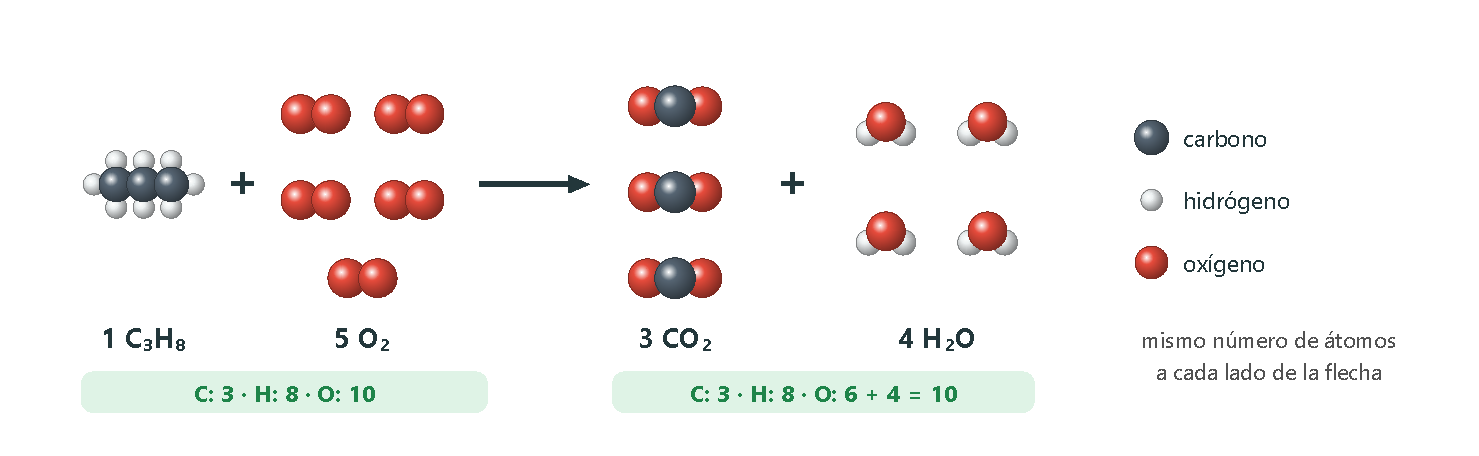
\includegraphics[width=0.9\textwidth]{images/UD6/ajuste_propano}
    \caption{Combustión del propano ajustada: a los dos lados hay 3 átomos de C, 8 de H y 10 de O.}
    \label{fig:ud6-propano}
\end{figure}

\begin{example}
    \textbf{Ajuste de la fotosíntesis.} Ajusta por tanteo la ecuación de la fotosíntesis:
    \ch{CO2 + H2O -> C6H12O6 + O2}.

    \textbf{Solución.} Carbono: 6 en la glucosa; ponemos un 6 delante del \ch{CO2}: \ch{6 CO2 + H2O -> C6H12O6 + O2}.
    Hidrógeno: 12 en la glucosa; ponemos un 6 delante del agua: \ch{6 CO2 + 6 H2O -> C6H12O6 + O2}. Oxígeno: a la izquierda hay
    \(6 \cdot 2 + 6 = 18\); a la derecha, 6 en la glucosa, así que faltan 12, es decir, 6 moléculas de \ch{O2}:
    \[ \ch{6 CO2 + 6 H2O -> C6H12O6 + 6 O2} \]
\end{example}

\begin{example}
    \textbf{Método algebraico.} Ajusta: \ch{NH3 + O2 -> NO + H2O}.

    \textbf{Solución.} \(a\,\ch{NH3} + b\,\ch{O2} \rightarrow c\,\ch{NO} + d\,\ch{H2O}\). N: \(a = c\); H: \(3a = 2d\); O: \(2b = c + d\). Con \(a = 1\):
    \(c = 1\), \(d = \frac{3}{2}\), \(b = \frac{5}{4}\). Multiplicamos todo por 4:
    \[ \ch{4 NH3 + 5 O2 -> 4 NO + 6 H2O} \]
\end{example}

\begin{exercise}
    Ajusta por tanteo estas reacciones: a) \ch{C5H12 + O2 -> CO2 + H2O}; b) \ch{SO2 + O2 -> SO3};
    c) \ch{HBr + Ca(OH)2 -> CaBr2 + H2O}; d) \ch{FeS2 + O2 -> Fe2O3 + SO2}; e) \ch{Ag2SO4 + KCl -> K2SO4 + AgCl};
    f) \ch{Mg + HCl -> MgCl2 + H2}; g) \ch{H3PO4 + KOH -> K3PO4 + H2O}.
    \begin{solu}
        a) \textcolor{red}{\ch{C5H12 + 8 O2 -> 5 CO2 + 6 H2O}}; b) \textcolor{red}{\ch{2 SO2 + O2 -> 2 SO3}};
        c) \textcolor{red}{\ch{2 HBr + Ca(OH)2 -> CaBr2 + 2 H2O}}; d) \textcolor{red}{\ch{4 FeS2 + 11 O2 -> 2 Fe2O3 + 8 SO2}};
        e) \textcolor{red}{\ch{Ag2SO4 + 2 KCl -> K2SO4 + 2 AgCl}}; f) \textcolor{red}{\ch{Mg + 2 HCl -> MgCl2 + H2}};
        g) \textcolor{red}{\ch{H3PO4 + 3 KOH -> K3PO4 + 3 H2O}}.
    \end{solu}
\end{exercise}

\begin{exercise}
    Ajusta por el método algebraico: a) la fermentación de la glucosa, \ch{C6H12O6 -> C2H5OH + CO2}; b) \ch{Cu + HNO3 ->
    Cu(NO3)2 + NO2 + H2O}.
    \begin{solu}
        a) \textcolor{blue}{C: \(6a = 2b + c\); H: \(12a = 6b\); O: \(6a = b + 2c\). Con \(a = 1\): \(b = 2\), \(c = 2\).}
        \textcolor{red}{\ch{C6H12O6 -> 2 C2H5OH + 2 CO2}}.
        b) \textcolor{blue}{\(a\,\ch{Cu} + b\,\ch{HNO3} \rightarrow c\,\ch{Cu(NO3)2} + d\,\ch{NO2} + e\,\ch{H2O}\). Cu: \(a = c\); H: \(b = 2e\); N: \(b = 2c + d\);
        O: \(3b = 6c + 2d + e\). Con \(a = c = 1\): \(b = 2 + d\) y \(3b = 6 + 2d + b/2\); resolviendo, \(b = 4\), \(d = 2\), \(e = 2\).}
        \textcolor{red}{\ch{Cu + 4 HNO3 -> Cu(NO3)2 + 2 NO2 + 2 H2O}}.
    \end{solu}
\end{exercise}

\begin{exercise}
    ¿Están ajustadas estas ecuaciones? Ajusta las que no lo estén: a) \ch{2 H2SO4 + S -> 3 SO2 + 2 H2O};
    b) \ch{2 HI + H2SO4 -> I2 + SO2 + 2 H2O}; c) \ch{2 KClO3 -> 2 KCl + 3 O2}; d) \ch{Fe2O3 + 2 CO -> 2 Fe + 2 CO2}.
    \begin{solu}
        \textcolor{red}{a), b) y c) están ajustadas.} d) \textcolor{blue}{Hay 5 O a la izquierda y 4 a la derecha.}
        \textcolor{red}{\ch{Fe2O3 + 3 CO -> 2 Fe + 3 CO2}}.
    \end{solu}
\end{exercise}

\subsection{Interpretación de la ecuación química}

Una vez ajustada, la ecuación da información cuantitativa: los coeficientes indican la proporción en que reaccionan y se forman
las sustancias, tanto en \textbf{moléculas} como en \textbf{moles} (al multiplicar todo por \(N_A\) la proporción no cambia) y,
si son gases en las mismas condiciones de presión y temperatura, en \textbf{volumen} (ley de Gay-Lussac). Con las masas molares,
la proporción en moles se convierte en proporción en \textbf{masa}.

\begin{table}[H]
    \centering
    \caption{Información de la ecuación ajustada de la combustión del propano}
    \vspace{-5pt}
    \begin{tabular}{@{}lcccc@{}}
        \toprule
        & \ch{C3H8(g)} & \ch{+ 5 O2(g)} & \ch{-> 3 CO2(g)} & \ch{+ 4 H2O(l)} \\
        \midrule
        Moléculas & 1 & 5 & 3 & 4 \\[3pt]
        Moles & 1 & 5 & 3 & 4 \\[3pt]
        Masa (g) & \(1 \cdot 44 = 44\) & \(5 \cdot 32 = 160\) & \(3 \cdot 44 = 132\) & \(4 \cdot 18 = 72\) \\[3pt]
        Volumen de gas (c.\,n.) & \qty{22.4}{\litre} & \qty{112}{\litre} & \qty{67.2}{\litre} & — (líquido) \\
        \bottomrule
    \end{tabular}
    \label{tab:ud6-interpretacion}
\end{table}

Fíjate en que la masa se conserva (\(44 + 160 = 132 + 72 = \qty{204}{\gram}\)), pero el número de moles no tiene por qué
conservarse (6 moles de reactivos dan 7 de productos).

\begin{example}
    \textbf{Leer una ecuación.} Ajusta e interpreta en moléculas, moles y gramos la reacción del hierro con el ácido clorhídrico:
    \ch{Fe(s) + HCl(aq) -> FeCl3(aq) + H2(g) ^}.

    \textbf{Solución.} Ajustada por tanteo: \ch{2 Fe(s) + 6 HCl(aq) -> 2 FeCl3(aq) + 3 H2(g) ^}.
    \begin{itemize}
        \item Dos átomos de hierro reaccionan con seis moléculas de \ch{HCl} para dar dos unidades de \ch{FeCl3} y tres moléculas
        de hidrógeno gaseoso, que se desprende.
        \item 2 mol de Fe reaccionan con 6 mol de \ch{HCl} y dan 2 mol de \ch{FeCl3} y 3 mol de \ch{H2}.
        \item Con las masas molares (Fe 55,8; \ch{HCl} 36,5; \ch{FeCl3} 162,3; \ch{H2} \qty{2}{\gram\per\mol}):
        \(\qty{111.6}{\gram}\) de Fe reaccionan con \qty{219}{\gram} de \ch{HCl} y dan \qty{324.6}{\gram} de \ch{FeCl3} y
        \qty{6}{\gram} de \ch{H2}. Se conserva la masa: \(\num{111.6} + 219 = \num{324.6} + 6 = \qty{330.6}{\gram}\).
    \end{itemize}
\end{example}

\begin{exercise}
    Ajusta y da toda la información cuantitativa (moles y gramos) de: a) \ch{Na + H2O -> NaOH + H2};
    b) \ch{Mg + H2SO4 -> MgSO4 + H2}; c) \ch{CH4 + O2 -> CO2 + H2O}.
    \begin{solu}
        a) \textcolor{red}{\ch{2 Na + 2 H2O -> 2 NaOH + H2}}: 2 mol (\qty{46}{\gram}) de Na y 2 mol (\qty{36}{\gram}) de agua dan
        2 mol (\qty{80}{\gram}) de \ch{NaOH} y 1 mol (\qty{2}{\gram}) de \ch{H2}; \(82 = 82\).
        b) \textcolor{red}{\ch{Mg + H2SO4 -> MgSO4 + H2}} (ya ajustada): \qty{24.3}{\gram} de Mg y \qty{98}{\gram} de ácido dan
        \qty{120.3}{\gram} de \ch{MgSO4} y \qty{2}{\gram} de \ch{H2}.
        c) \textcolor{red}{\ch{CH4 + 2 O2 -> CO2 + 2 H2O}}: \qty{16}{\gram} de metano y \qty{64}{\gram} de oxígeno dan
        \qty{44}{\gram} de \ch{CO2} y \qty{36}{\gram} de agua; \(80 = 80\).
    \end{solu}
\end{exercise}

\begin{exercise}
    En la reacción \ch{N2(g) + 3 H2(g) -> 2 NH3(g)}, ¿qué volumen de hidrógeno reacciona con \qty{12}{\litre} de nitrógeno?
    ¿Qué volumen de amoníaco se forma? Todos los gases están en las mismas condiciones.
    \begin{solu}
        \textcolor{blue}{En las mismas condiciones, la proporción en volumen es la de los coeficientes: 1 : 3 : 2.}
        \textcolor{red}{\qty{36}{\litre} de \ch{H2} y \qty{24}{\litre} de \ch{NH3}}.
    \end{solu}
\end{exercise}

%========================================================================================
\section{Tipos de reacciones químicas}\label{sec:ud6-tipos}
%========================================================================================

Las reacciones se pueden clasificar con muchos criterios: por su \textbf{velocidad} (rápidas o lentas), por la \textbf{energía}
que intercambian (exotérmicas o endotérmicas), por el \textbf{mecanismo} o por las \textbf{partículas que se transfieren}. Vamos a
estudiar estos dos últimos.

\subsection{Según el mecanismo de reacción}

\begin{figure}[H]
    \centering
    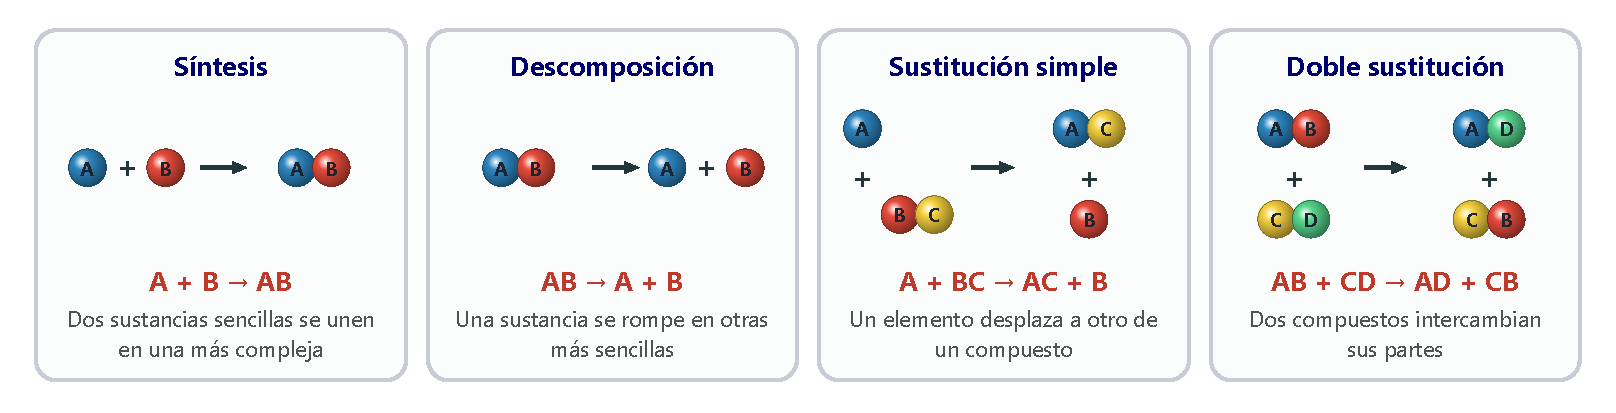
\includegraphics[width=\textwidth]{images/UD6/tipos_reaccion}
    \caption{Los cuatro tipos de reacción según su mecanismo.}
    \label{fig:ud6-tipos}
\end{figure}

\paragraph{Síntesis (\ch{A + B -> AB}).} Dos o más reactivos sencillos se combinan para dar un compuesto más complejo. Tienen un
gran interés industrial: así se obtienen medicamentos, plásticos o cosméticos. Por ejemplo, la síntesis del metanol, un
disolvente y combustible, \ch{CO(g) + 2 H2(g) -> CH3OH(g)}, o la del amoníaco, \ch{N2(g) + 3 H2(g) -> 2 NH3(g)}. Si se
obtiene un mol de compuesto a partir de sus elementos en su forma natural, se llama \textbf{reacción de formación}.

\paragraph{Descomposición (\ch{AB -> A + B}).} Una sustancia se rompe en otras más sencillas; es el proceso inverso de la
síntesis. El ácido carbónico de los refrescos se descompone en agua y \ch{CO2} (las burbujas), \ch{H2CO3(aq) -> H2O(l) + CO2(g)},
y el ácido nítrico se descompone con la luz, \ch{4 HNO3(l) -> 4 NO2(g) + O2(g) + 2 H2O(l)}; el \ch{NO2} es el gas pardo que da
color anaranjado al aire contaminado.

\paragraph{Sustitución o desplazamiento simple (\ch{A + BC -> AC + B}).} Un elemento sustituye a otro en un compuesto. Es el
caso de la \textbf{reacción termita}, \ch{2 Al + Fe2O3 -> Al2O3 + 2 Fe}, que desprende tanto calor que el hierro sale fundido;
se usa para soldar raíles.

\paragraph{Doble sustitución (\ch{AB + CD -> AD + CB}).} Dos compuestos intercambian sus partes. Al mezclar disoluciones de
nitrato de plomo(II) y de yoduro de potasio se forma yoduro de plomo(II), un sólido amarillo que precipita:
\ch{Pb(NO3)2(aq) + 2 KI(aq) -> PbI2(s) v + 2 KNO3(aq)}.

\begin{example}
    \textbf{Clasificar reacciones.} Clasifica según su mecanismo: a) \ch{2 Al + 3 S -> Al2S3};
    b) \ch{Ca(OH)2 -> CaO + H2O}; c) \ch{2 Li + 2 H2O -> 2 LiOH + H2}; d) \ch{BaCl2 + Na2SO4 -> BaSO4 + 2 NaCl}.

    \textbf{Solución.} a) \textbf{Síntesis}: dos elementos se unen en un compuesto. b) \textbf{Descomposición}: un compuesto da dos
    más sencillos. c) \textbf{Sustitución simple}: el litio desplaza a uno de los hidrógenos del agua. d) \textbf{Doble
    sustitución}: el bario y el sodio intercambian sus aniones.
\end{example}

\begin{exercise}
    Clasifica según su mecanismo: a) \ch{4 Al + 3 O2 -> 2 Al2O3}; b) \ch{CaCO3 -> CaO + CO2};
    c) \ch{Zn + CuSO4 -> ZnSO4 + Cu}; d) \ch{AgNO3 + NaCl -> AgCl + NaNO3}; e) \ch{2 H2O2 -> 2 H2O + O2};
    f) \ch{Cl2 + 2 KBr -> 2 KCl + Br2}.
    \begin{solu}
        \textcolor{red}{Síntesis: a). Descomposición: b) y e). Sustitución simple: c) y f). Doble sustitución: d).}
    \end{solu}
\end{exercise}

\subsection{Según las partículas que se transfieren}

\subsubsection{Reacciones ácido-base: transferencia de protones}

Según la teoría de \textbf{Brønsted y Lowry}:

\begin{definition}[Ácidos y bases]
    Un \textbf{ácido} es una sustancia capaz de \textbf{ceder protones} (\ch{H+}); en agua produce iones hidronio, \ch{H3O+}.

    Una \textbf{base} es una sustancia capaz de \textbf{captar protones}; en agua produce iones hidróxido, \ch{OH-}.
\end{definition}

El cloruro de hidrógeno se disocia por completo en agua, \ch{HCl + H2O -> H3O+ + Cl-}: es un \textbf{ácido fuerte}. El
amoníaco capta protones del agua, \ch{NH3 + H2O <=> NH4+ + OH-}, pero solo en pequeña proporción: es una \textbf{base débil}.

\begin{table}[H]
    \centering
    \caption{Propiedades de los ácidos y de las bases}
    \vspace{-5pt}
    \begin{tabular}{@{}L{6.6cm}L{6.6cm}@{}}
        \toprule
        \textbf{Ácidos} & \textbf{Bases} \\
        \midrule
        Sabor agrio (limón, vinagre) & Sabor amargo \\[3pt]
        Son corrosivos & Son cáusticos: pueden quemar la piel \\[3pt]
        Atacan a metales como Fe, Zn o Mg desprendiendo \ch{H2} & Tacto suave, jabonoso \\[3pt]
        Con la caliza (\ch{CaCO3}) desprenden \ch{CO2}: «prueba del ácido» de los geólogos & Neutralizan a los ácidos \\
        \bottomrule
    \end{tabular}
    \label{tab:ud6-acidos}
\end{table}

\paragraph{La escala de pH.} La acidez de una disolución depende de su concentración de \ch{H3O+}. Como esta concentración varía
mucho, se usa una escala logarítmica, el \textbf{pH}: \(\mathrm{pH} = -\log\,[\ch{H3O+}]\). El agua pura y las disoluciones
neutras tienen pH 7; las ácidas, menos de 7, y las básicas, más de 7. Cada unidad de pH supone una concentración de \ch{H3O+} diez
veces mayor o menor.

\begin{figure}[H]
    \centering
    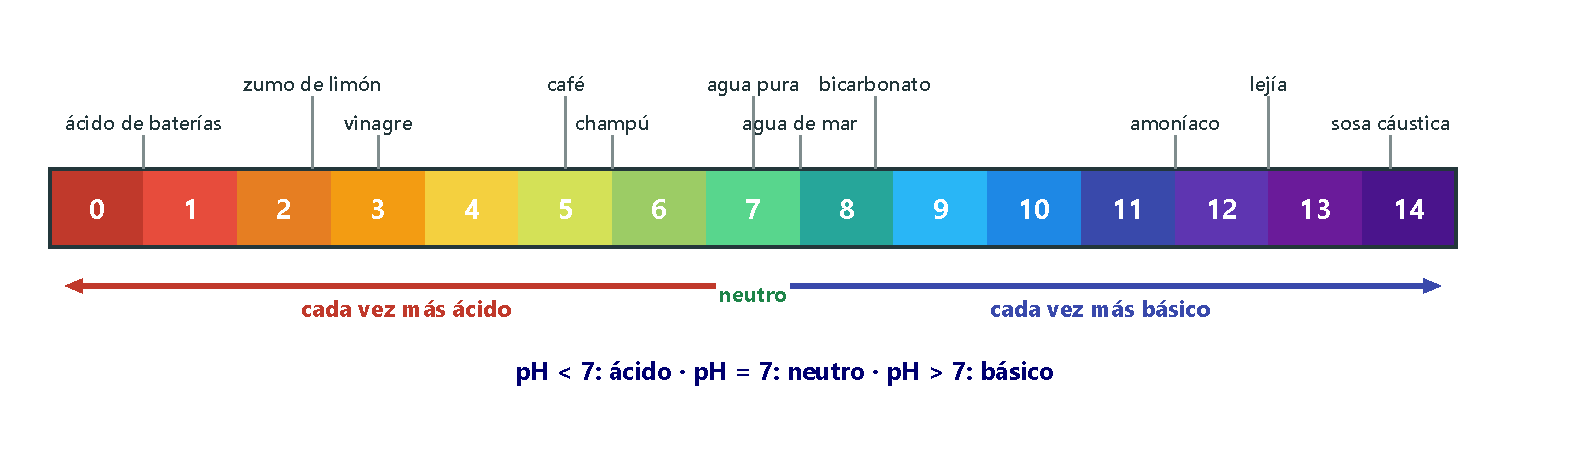
\includegraphics[width=0.9\textwidth]{images/UD6/escala_ph}
    \caption{Escala de pH de algunas sustancias de uso cotidiano.}
    \label{fig:ud6-ph}
\end{figure}

\paragraph{Reacciones de neutralización.} Cuando un ácido y una base reaccionan, el ácido transfiere protones a la base y se
forman una \textbf{sal} y \textbf{agua}; ambos pierden sus propiedades características: se \textbf{neutralizan}.
\[ \text{ácido} + \text{base} \ch{->} \text{sal} + \text{agua} \qquad\qquad \ch{HCl + NaOH -> NaCl + H2O} \]
Por ejemplo, los antiácidos (bicarbonato de sodio, hidróxido de magnesio) son bases que neutralizan el exceso de ácido clorhídrico
del estómago.

\begin{example}
    \textbf{Picaduras.} Las avispas inyectan con su picadura una sustancia básica y las hormigas, ácido fórmico. ¿Qué pondrías sobre
    cada picadura para aliviarla?

    \textbf{Solución.} Una sustancia de carácter contrario, que la neutralice: sobre la picadura de avispa, un ácido débil, como el
    vinagre o el zumo de limón; sobre la de hormiga, una base débil, como bicarbonato disuelto en agua o amoníaco diluido. En los dos
    casos se produce una neutralización: ácido + base \(\rightarrow\) sal + agua.
\end{example}

\begin{exercise}
    Completa y ajusta estas neutralizaciones: a) \ch{Al(OH)3 + HBr ->}; b) \ch{H2SO4 + KOH ->};
    c) \ch{Ca(OH)2 + HNO3 ->}; d) \ch{HCl + Fe(OH)3 ->}; e) \ch{NH3 + HCl ->}; f) \ch{CH3COOH + KOH ->}.
    \begin{solu}
        a) \textcolor{red}{\ch{Al(OH)3 + 3 HBr -> AlBr3 + 3 H2O}}; b) \textcolor{red}{\ch{H2SO4 + 2 KOH -> K2SO4 + 2 H2O}};
        c) \textcolor{red}{\ch{Ca(OH)2 + 2 HNO3 -> Ca(NO3)2 + 2 H2O}}; d) \textcolor{red}{\ch{3 HCl + Fe(OH)3 -> FeCl3 + 3 H2O}};
        e) \textcolor{red}{\ch{NH3 + HCl -> NH4Cl}} (el amoníaco capta el protón y no se forma agua);
        f) \textcolor{red}{\ch{CH3COOH + KOH -> CH3COOK + H2O}}.
    \end{solu}
\end{exercise}

\begin{exercise}
    a) El zumo de limón tiene pH 2 y el café, pH 5. ¿Cuántas veces mayor es la concentración de \ch{H3O+} en el limón? b) Escribe la
    reacción con la que un antiácido de hidróxido de magnesio neutraliza el ácido del estómago.
    \begin{solu}
        a) \textcolor{blue}{Tres unidades de pH equivalen a un factor \(10^3\).} \textcolor{red}{1000 veces mayor}.
        b) \textcolor{red}{\ch{Mg(OH)2 + 2 HCl -> MgCl2 + 2 H2O}}.
    \end{solu}
\end{exercise}

\subsubsection{Reacciones redox: transferencia de electrones}

\begin{definition}[Oxidación y reducción]
    En una reacción \textbf{redox} una sustancia \textbf{pierde electrones} y otra los \textbf{gana}.
    \begin{itemize}
        \item La sustancia que pierde electrones \textbf{se oxida}; es el \textbf{reductor}, porque reduce a la otra.
        \item La sustancia que gana electrones \textbf{se reduce}; es el \textbf{oxidante}.
    \end{itemize}
\end{definition}

En la oxidación del hierro por el oxígeno del aire, \ch{4 Fe + 3 O2 -> 2 Fe2O3}, cada proceso se puede escribir por separado
en una \textbf{semirreacción}:
\[ \text{oxidación: } \ch{Fe -> Fe^3+ + 3 e-} \qquad\qquad \text{reducción: } \ch{O2 + 4 e- -> 2 O^2-} \]
El Fe se oxida (es el reductor) y el \ch{O2} se reduce (es el oxidante). La oxidación y la reducción \textbf{ocurren siempre a la
vez}: los electrones que pierde una sustancia los gana la otra. Para obtener la ecuación global, se multiplica cada semirreacción
por un número de forma que los electrones perdidos y ganados sean los mismos (aquí, 12) y se suman: \(4 \cdot (\ch{Fe -> Fe^3+ +
3 e-})\) y \(3 \cdot (\ch{O2 + 4 e- -> 2 O^2-})\) dan \ch{4 Fe + 3 O2 -> 2 Fe2O3}.

Las reacciones redox están por todas partes: las \textbf{combustiones}, la respiración, la corrosión de los metales y su protección,
la \textbf{obtención de metales} a partir de sus minerales y el funcionamiento de \textbf{pilas y baterías}.

\begin{remark}
    \textbf{La pila Daniell.} Si el zinc y los iones \ch{Cu^2+} están en recipientes separados, \ch{Zn + CuSO4 -> ZnSO4 + Cu},
    los electrones que pierde el zinc tienen que viajar por un cable para llegar al cobre: se genera una \textbf{corriente
    eléctrica}. Así funciona una pila: una reacción redox convierte energía química en eléctrica.
\end{remark}

\begin{exercise}
    En estas reacciones redox, escribe las semirreacciones e indica el oxidante y el reductor: a) \ch{S + O2 -> SO2};
    b) \ch{2 Fe + 3 Cl2 -> 2 FeCl3}; c) \ch{Zn + 2 HCl -> ZnCl2 + H2}.
    \begin{solu}
        a) \textcolor{blue}{\ch{S -> S^4+ + 4 e-} (oxidación); \ch{O2 + 4 e- -> 2 O^2-} (reducción).} \textcolor{red}{Reductor: S;
        oxidante: \ch{O2}.} b) \textcolor{blue}{\ch{Fe -> Fe^3+ + 3 e-}; \ch{Cl2 + 2 e- -> 2 Cl-}.} \textcolor{red}{Reductor: Fe;
        oxidante: \ch{Cl2}.} c) \textcolor{blue}{\ch{Zn -> Zn^2+ + 2 e-}; \ch{2 H+ + 2 e- -> H2}.} \textcolor{red}{Reductor: Zn;
        oxidante: \ch{H+} (del \ch{HCl}).}
    \end{solu}
\end{exercise}

\subsubsection{Reacciones de precipitación: transferencia de iones}

En estas reacciones, iones presentes en una \textbf{disolución acuosa} se combinan y forman una \textbf{sustancia insoluble}, el
\textbf{precipitado}, que enturbia el líquido y acaba depositándose en el fondo. Por ejemplo, al mezclar nitrato de plata y
cromato de sodio se forma cromato de plata, rojo e insoluble:
\[ \ch{2 AgNO3(aq) + Na2CrO4(aq) -> Ag2CrO4(s) v + 2 NaNO3(aq)} \]
Este precipitado se usa en el \textbf{método de Golgi} para teñir las neuronas y poder verlas al microscopio.

Las reacciones de precipitación sirven para \textbf{eliminar metales} de las aguas residuales, para \textbf{analizar} qué iones
contiene una muestra o, en inmunología, en las pruebas serológicas, en las que un antígeno y sus anticuerpos forman un precipitado.
Otras veces son indeseadas: el \ch{CaCO3} que precipita en las tuberías (la cal) las obstruye y estropea calentadores y
electrodomésticos.

\begin{example}
    \textbf{Doble clasificación.} Ajusta y clasifica según su mecanismo y según la partícula transferida:
    a) \ch{K2SO4 + CaBr2 -> KBr + CaSO4 v}; b) \ch{HgO -> Hg + O2}.

    \textbf{Solución.} a) \ch{K2SO4 + CaBr2 -> 2 KBr + CaSO4 v}. Es una \textbf{doble sustitución} y, como el \ch{CaSO4} es poco
    soluble y precipita, una reacción de \textbf{precipitación}.

    b) \ch{2 HgO -> 2 Hg + O2}. Es una \textbf{descomposición} y una reacción \textbf{redox}: el mercurio gana electrones (se
    reduce) y el oxígeno los pierde (se oxida):
    \[ 2 \cdot (\ch{Hg^2+ + 2 e- -> Hg}) \qquad\quad \ch{2 O^2- -> O2 + 4 e-} \]
\end{example}

\begin{exercise}
    Ajusta y clasifica estas reacciones según los dos criterios que hemos visto: a) \ch{Cu(NO3)2 -> CuO + NO2 + O2};
    b) \ch{K2CO3 + CaCl2 -> KCl + CaCO3 v}; c) \ch{Fe + Cl2 -> FeCl3}.
    \begin{solu}
        a) \textcolor{red}{\ch{2 Cu(NO3)2 -> 2 CuO + 4 NO2 + O2}}: descomposición y redox (el N se reduce y parte del O se oxida).
        b) \textcolor{red}{\ch{K2CO3 + CaCl2 -> 2 KCl + CaCO3 v}}: doble sustitución y precipitación.
        c) \textcolor{red}{\ch{2 Fe + 3 Cl2 -> 2 FeCl3}}: síntesis y redox (el Fe se oxida y el \ch{Cl2} se reduce).
    \end{solu}
\end{exercise}

%========================================================================================
\section{Cálculos estequiométricos}\label{sec:ud6-estequiometria}
%========================================================================================

En el laboratorio, en la industria y hasta en la cocina es necesario saber qué cantidad de cada sustancia hace falta o se obtiene en
un proceso. Si una receta de bizcocho para 8 personas lleva 4 huevos y \qty{200}{\gram} de harina, para 4 personas necesitarás la
mitad de todo: la receta fija una proporción. En química, esa proporción la dan los coeficientes de la ecuación ajustada.

\begin{definition}[Cálculos estequiométricos]
    Son los cálculos que permiten conocer las cantidades de reactivos y productos que intervienen en una reacción a partir de su
    \textbf{ecuación ajustada}.
\end{definition}

Para resolver un problema de estequiometría, identifica primero el \textbf{dato} y la \textbf{incógnita} y sigue el esquema de la
figura~\ref{fig:ud6-esquema}. El paso clave, común a todos los problemas, es el 3: la relación entre moles que dan los coeficientes.

\begin{figure}[H]
    \centering
    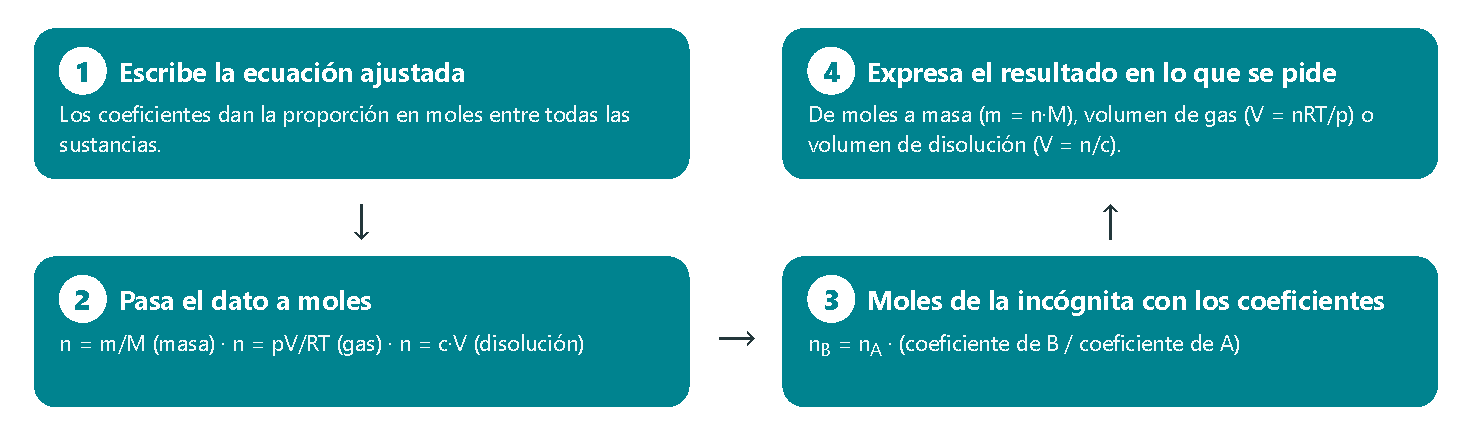
\includegraphics[width=0.85\textwidth]{images/UD6/esquema_estequiometria}
    \caption{Pasos para resolver un problema de estequiometría.}
    \label{fig:ud6-esquema}
\end{figure}

\begin{example}
    \textbf{Factor de conversión o proporción.} El agua oxigenada se descompone en agua y oxígeno:
    \ch{H2O2(aq) -> H2O(l) + 1/2 O2(g)}. ¿Cuánto oxígeno se desprende al descomponerse \qty{3}{\mol} de agua oxigenada? ¿Qué
    masa es?

    \textbf{Solución.} Dato: \qty{3}{\mol} de \ch{H2O2}; incógnita: el \ch{O2}. Por cada mol de \ch{H2O2} se forma \(\frac{1}{2}\) mol
    de \ch{O2}. Podemos usar un \textbf{factor de conversión}:
    \[ \qty{3}{\mol}\ \ch{H2O2} \cdot \frac{\frac{1}{2}\ \unit{\mol}\ \ch{O2}}{\qty{1}{\mol}\ \ch{H2O2}} = \qty{1.5}{\mol}\ \ch{O2} \]
    o una \textbf{proporción}: \(\dfrac{1}{1/2} = \dfrac{3}{x} \Rightarrow x = \qty{1.5}{\mol}\). Su masa es
    \(m = n \cdot M = \num{1.5} \cdot 32 = \qty{48}{\gram}\) de \ch{O2}.
\end{example}

\subsection{Cálculos con masas y volúmenes de gases}

En los pasos 2 y 4 hay que pasar de masa o volumen a moles y al revés. Recuerda:
\begin{itemize}
    \item \textbf{Masa}: \(n = \dfrac{m}{M}\). Si es un sólido o un líquido del que conocemos el volumen, primero se calcula la masa
    con la densidad, \(m = d \cdot V\).
    \item \textbf{Gases}: \(n = \dfrac{p\,V}{R\,T}\), con \(R = \qty{0.082}{\atm\litre\per\mol\per\kelvin}\). En
    \textbf{condiciones normales} (c.\,n.: \qty{0}{\degreeCelsius} y \qty{1}{\atm}), un mol de cualquier gas ocupa
    \qty{22.4}{\litre}. Recuerda también que \(\qty{1}{\atm} = \qty{1.013e5}{\pascal} = \qty{760}{\mmHg}\).
    \item Si los reactivos y productos son \textbf{gases en las mismas condiciones} de presión y temperatura, los coeficientes dan
    directamente la proporción entre sus volúmenes.
\end{itemize}

\begin{example}
    \textbf{De masa a volumen de gas.} Se hacen reaccionar \qty{20.0}{\gram} de zinc con ácido clorhídrico en exceso:
    \ch{Zn + 2 HCl -> ZnCl2 + H2 ^}. ¿Qué volumen de hidrógeno se obtiene a \qty{25}{\degreeCelsius} y \qty{740}{\mmHg}?

    \textbf{Solución.} \textbf{1.} La ecuación ya está ajustada. \textbf{2.} Moles de Zn: \(n = \dfrac{\qty{20.0}{\gram}}{\qty{65.4}{\gram\per\mol}} =
    \qty{0.306}{\mol}\). \textbf{3.} Por cada mol de Zn se forma 1 mol de \ch{H2}:
    \[ \qty{0.306}{\mol}\ \ch{Zn} \cdot \frac{\qty{1}{\mol}\ \ch{H2}}{\qty{1}{\mol}\ \ch{Zn}} = \qty{0.306}{\mol}\ \ch{H2} \]
    \textbf{4.} Con \(p = \dfrac{740}{760} = \qty{0.974}{\atm}\) y \(T = 25 + 273 = \qty{298}{\kelvin}\):
    \[ V = \frac{n R T}{p} = \frac{\num{0.306} \cdot \num{0.082} \cdot 298}{\num{0.974}} = \qty{7.67}{\litre}\ \text{de}\ \ch{H2} \]
\end{example}

\begin{example}
    \textbf{De volumen de gas a masa.} Con la misma reacción, ¿qué masa de \ch{HCl} hace falta para obtener \qty{15}{\litre} de
    \ch{H2} medidos en condiciones normales?

    \textbf{Solución.} Encadenamos los factores de conversión, partiendo siempre del dato:
    \[ \qty{15}{\litre}\ \ch{H2} \cdot \frac{\qty{1}{\mol}\ \ch{H2}}{\qty{22.4}{\litre}\ \ch{H2}} \cdot
    \frac{\qty{2}{\mol}\ \ch{HCl}}{\qty{1}{\mol}\ \ch{H2}} \cdot \frac{\qty{36.5}{\gram}\ \ch{HCl}}{\qty{1}{\mol}\ \ch{HCl}} =
    \qty{48.9}{\gram}\ \ch{HCl} \]
\end{example}

\begin{exercise}
    Calcula el volumen de \ch{CO2}, medido a \qty{5}{\degreeCelsius} y \qty{600}{\mmHg}, que se produce al quemar \qty{50}{\gram}
    de butano, \ch{C4H10}.
    \begin{solu}
        \textcolor{blue}{\ch{2 C4H10 + 13 O2 -> 8 CO2 + 10 H2O}; \(n(\ch{C4H10}) = 50/58 = \qty{0.862}{\mol}\);
        \(n(\ch{CO2}) = 4 \cdot \num{0.862} = \qty{3.45}{\mol}\); \(p = 600/760 = \qty{0.789}{\atm}\).}
        \(V = \dfrac{\num{3.45} \cdot \num{0.082} \cdot 278}{\num{0.789}} = \textcolor{red}{\qty{99.6}{\litre}}\).
    \end{solu}
\end{exercise}

\begin{exercise}
    Se hacen reaccionar \qty{8.0}{\gram} de ácido sulfúrico con zinc en exceso, y se obtienen sulfato de zinc e hidrógeno.
    a) Escribe y ajusta la reacción. b) ¿Qué masa de hidrógeno se forma? c) ¿Qué volumen ocupa a \qty{27}{\degreeCelsius} y
    \qty{720}{\mmHg}?
    \begin{solu}
        a) \textcolor{red}{\ch{Zn + H2SO4 -> ZnSO4 + H2}}. b) \textcolor{blue}{\(n(\ch{H2SO4}) = 8/98 = \qty{0.0816}{\mol} = n(\ch{H2})\).}
        \(m = \num{0.0816} \cdot 2 = \textcolor{red}{\qty{0.163}{\gram}}\). c) \(V = \dfrac{\num{0.0816} \cdot \num{0.082} \cdot 300}{720/760}
        = \textcolor{red}{\qty{2.12}{\litre}}\).
    \end{solu}
\end{exercise}

\begin{exercise}
    Con la reacción del ejercicio anterior, ¿qué masa de zinc se necesita para obtener \qty{30}{\litre} de hidrógeno en condiciones
    normales?
    \begin{solu}
        \(\dfrac{30}{\num{22.4}} = \qty{1.34}{\mol}\) de \ch{H2} \(=\) mol de Zn; \(m = \num{1.34} \cdot \num{65.4} =
        \textcolor{red}{\qty{87.6}{\gram}}\) de Zn.
    \end{solu}
\end{exercise}

\subsection{Cálculos con disoluciones}

Muchas reacciones, en el laboratorio, en la industria y en los seres vivos, tienen lugar en \textbf{disolución acuosa}. Hay que
recordar que la sustancia que reacciona es el \textbf{soluto}; el disolvente, en general, no interviene. En los pasos 2 y 4 se
relaciona la cantidad de soluto con la concentración (unidad 2):
\[ \%\,\text{masa} = \frac{m_{\text{soluto}}}{m_{\text{disolución}}} \cdot 100 \qquad
c = \frac{n_{\text{soluto}}}{V_{\text{disolución}}} \qquad \gamma = \frac{m_{\text{soluto}}}{V_{\text{disolución}}} \]
A veces, sin embargo, el agua es también reactivo o producto: lee con atención el enunciado.

\begin{example}
    \textbf{Neutralización.} El hidróxido de magnesio reacciona con el ácido clorhídrico para dar cloruro de magnesio y agua.
    a) ¿Qué masa de ácido clorhídrico del 36\,\% en masa se necesita para neutralizar \qty{120}{\gram} de \ch{Mg(OH)2}?
    b) ¿Qué volumen se necesitaría si se usara ácido clorhídrico \qty{1.5}{\mol\per\litre}?

    \textbf{Solución.} \ch{Mg(OH)2 + 2 HCl -> MgCl2 + 2 H2O}; \(M(\ch{Mg(OH)2}) = \qty{58.3}{\gram\per\mol}\);
    \(M(\ch{HCl}) = \qty{36.5}{\gram\per\mol}\).

    a) \[ \qty{120}{\gram}\ \ch{Mg(OH)2} \cdot \frac{\qty{1}{\mol}}{\qty{58.3}{\gram}} \cdot \frac{\qty{2}{\mol}\ \ch{HCl}}{\qty{1}{\mol}\ \ch{Mg(OH)2}}
    = \qty{4.12}{\mol}\ \ch{HCl} \ \rightarrow\ \num{4.12} \cdot \num{36.5} = \qty{150.3}{\gram}\ \ch{HCl} \]
    Como el ácido solo tiene un 36\,\% de \ch{HCl}: \(\qty{150.3}{\gram}\ \ch{HCl} \cdot \dfrac{\qty{100}{\gram}\ \text{dis.}}{\qty{36}{\gram}\ \ch{HCl}} =
    \qty{417}{\gram}\) de disolución.

    b) \(V = \dfrac{n}{c} = \dfrac{\qty{4.12}{\mol}}{\qty{1.5}{\mol\per\litre}} = \qty{2.74}{\litre}\).
\end{example}

\begin{remark}
    \textbf{Volumetrías.} Una \textbf{valoración} o volumetría es una técnica de análisis para conocer la concentración de una
    disolución. Se añade gota a gota, con una bureta, una disolución de concentración conocida hasta que la reacción termina, lo que
    se detecta con un \textbf{indicador} que cambia de color. Con el volumen gastado y la estequiometría se calcula la concentración
    desconocida (figura~\ref{fig:ud6-valoracion}).
\end{remark}

\begin{figure}[H]
    \centering
    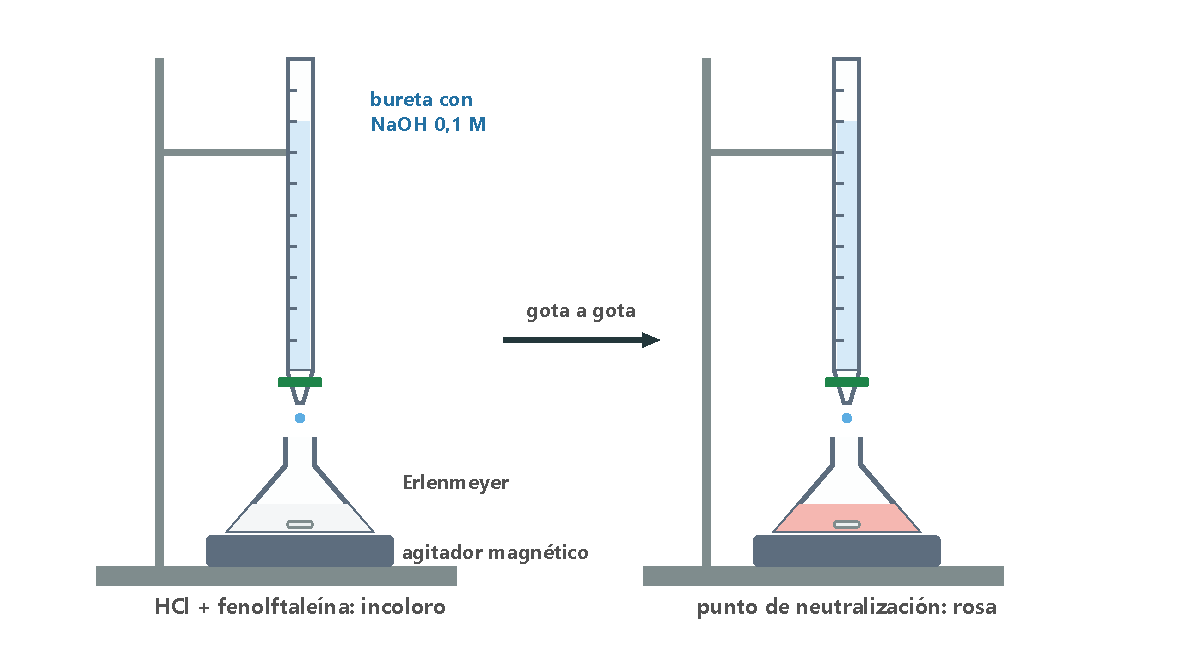
\includegraphics[width=0.62\textwidth]{images/UD6/valoracion}
    \caption{Valoración de un ácido con una base: la fenolftaleína se vuelve rosa al completarse la neutralización.}
    \label{fig:ud6-valoracion}
\end{figure}

\begin{exercise}
    Calcula el volumen de ácido clorhídrico \qty{0.5}{\mol\per\litre} necesario para neutralizar \qty{400}{\mL} de una disolución
    de hidróxido de calcio \qty{0.2}{\mol\per\litre}.
    \begin{solu}
        \textcolor{blue}{\ch{Ca(OH)2 + 2 HCl -> CaCl2 + 2 H2O}; \(n(\ch{Ca(OH)2}) = \num{0.4} \cdot \num{0.2} = \qty{0.08}{\mol}\);
        \(n(\ch{HCl}) = \qty{0.16}{\mol}\).} \(V = \num{0.16}/\num{0.5} = \textcolor{red}{\qty{0.32}{\litre} = \qty{320}{\mL}}\).
    \end{solu}
\end{exercise}

\begin{exercise}
    El nitrato de plata reacciona con el cloruro de sodio y precipita cloruro de plata. a) Escribe y ajusta la reacción. b) ¿Qué
    volumen de \ch{AgNO3} \qty{0.5}{\mol\per\litre} reacciona con \qty{200}{\mL} de \ch{NaCl} \qty{1.2}{\mol\per\litre}? c) ¿Qué
    masa de precipitado se obtiene?
    \begin{solu}
        a) \textcolor{red}{\ch{AgNO3 + NaCl -> AgCl v + NaNO3}}. b) \textcolor{blue}{\(n(\ch{NaCl}) = \num{0.2} \cdot \num{1.2} =
        \qty{0.24}{\mol} = n(\ch{AgNO3})\).} \(V = \num{0.24}/\num{0.5} = \textcolor{red}{\qty{480}{\mL}}\).
        c) \(\num{0.24} \cdot \num{143.4} = \textcolor{red}{\qty{34.4}{\gram}}\) de \ch{AgCl}.
    \end{solu}
\end{exercise}

\subsection{Reactivo limitante}

Los coeficientes de la ecuación ajustada dan la proporción \textbf{fija} en que se combinan los reactivos. Si las cantidades que
mezclamos no guardan esa proporción, la reacción se detiene cuando se acaba uno de ellos y del otro sobra una parte
(figura~\ref{fig:ud6-limitante}).

\begin{definition}[Reactivo limitante]
    Es el reactivo que \textbf{se agota primero} y, por tanto, el que determina la cantidad de productos que se forma. El que no se
    agota es el \textbf{reactivo en exceso}. Cuál es cada uno depende de las cantidades iniciales.
\end{definition}

\begin{figure}[H]
    \centering
    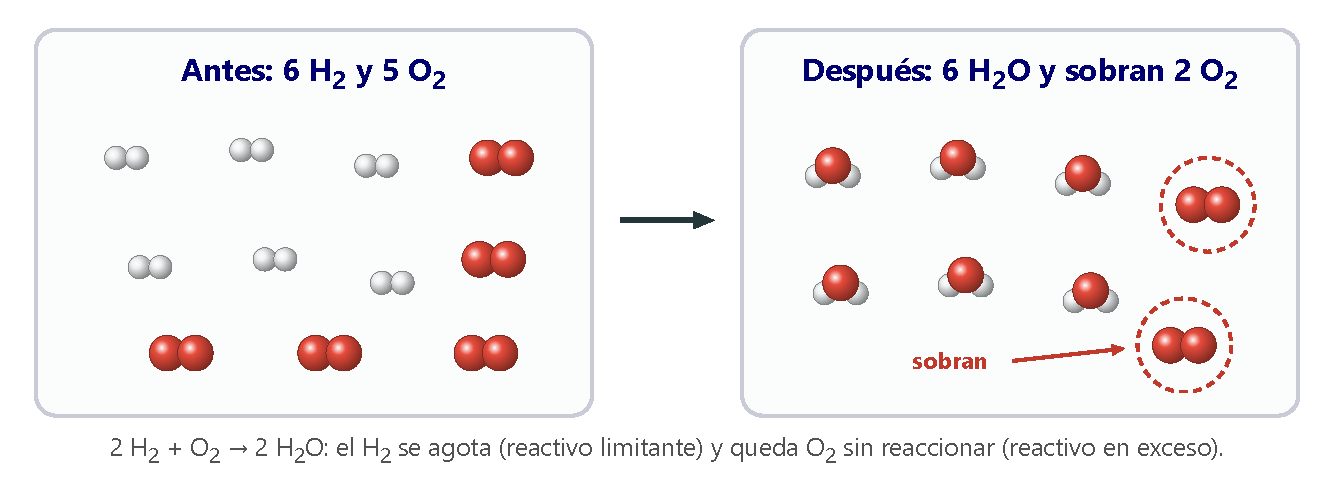
\includegraphics[width=0.8\textwidth]{images/UD6/reactivo_limitante}
    \caption{Con 6 moléculas de \ch{H2} y 5 de \ch{O2} solo se forman 6 de agua: el hidrógeno es el reactivo limitante.}
    \label{fig:ud6-limitante}
\end{figure}

Para una reacción \(a\,\ch{A} + b\,\ch{B} \rightarrow c\,\ch{C}\), hay dos formas de encontrar el reactivo limitante:
\begin{itemize}
    \item \textbf{Método 1.} Calcula los moles iniciales, \(n_A\) y \(n_B\). Con los coeficientes, calcula los moles de B que
    reaccionarían con todo A: \(n_B' = n_A \cdot \frac{b}{a}\). Si hay menos B de lo necesario (\(n_B < n_B'\)), \textbf{B es el
    limitante}; si hay más (\(n_B > n_B'\)), \textbf{A es el limitante}.
    \item \textbf{Método 2.} Calcula cuánto producto se obtendría si reaccionase todo A (\(n_A \cdot \frac{c}{a}\)) y si reaccionase
    todo B (\(n_B \cdot \frac{c}{b}\)). El limitante es el que da \textbf{menos} producto.
\end{itemize}
A partir de ese momento, todos los cálculos se hacen con la cantidad del reactivo limitante.

\begin{example}
    \textbf{Tricloruro de aluminio.} En un recipiente se introducen \qty{4}{\mol} de aluminio y \qty{5}{\mol} de cloro, que
    reaccionan para dar \ch{AlCl3}. a) ¿Cuál es el reactivo limitante? b) ¿Cuánto sobra del otro? c) ¿Cuántos moles de \ch{AlCl3} se
    forman?

    \textbf{Solución.} \ch{2 Al + 3 Cl2 -> 2 AlCl3}.

    a) Cloro necesario para que reaccione todo el aluminio: \(\qty{4}{\mol}\ \ch{Al} \cdot \dfrac{\qty{3}{\mol}\ \ch{Cl2}}{\qty{2}{\mol}\ \ch{Al}} =
    \qty{6}{\mol}\ \ch{Cl2}\). Solo hay 5: \textbf{el cloro es el limitante} y el aluminio está en exceso.

    b) Aluminio que reacciona: \(\qty{5}{\mol}\ \ch{Cl2} \cdot \dfrac{2}{3} = \qty{3.33}{\mol}\); sobran \(4 - \num{3.33} = \qty{0.67}{\mol}\) de Al.

    c) Con el limitante: \(\qty{5}{\mol}\ \ch{Cl2} \cdot \dfrac{2}{3} = \qty{3.33}{\mol}\) de \ch{AlCl3}.
\end{example}

\begin{example}
    \textbf{Con masas.} Se mezclan \qty{20}{\gram} de hidrógeno y \qty{64}{\gram} de oxígeno y se hace saltar una chispa:
    \ch{2 H2 + O2 -> 2 H2O}. ¿Qué masa de agua se forma? ¿Qué sobra?

    \textbf{Solución.} \(n(\ch{H2}) = 20/2 = \qty{10}{\mol}\); \(n(\ch{O2}) = 64/32 = \qty{2}{\mol}\). Para \qty{2}{\mol} de \ch{O2}
    hacen falta \qty{4}{\mol} de \ch{H2}, y hay 10: \textbf{el oxígeno es el limitante}. Se forman \(2 \cdot 2 = \qty{4}{\mol}\) de
    agua, es decir, \(4 \cdot 18 = \qty{72}{\gram}\), y sobran \(10 - 4 = \qty{6}{\mol}\) de \ch{H2} (\qty{12}{\gram}). Comprobamos:
    \(20 + 64 = 72 + 12\).
\end{example}

\begin{exercise}
    El cobre reacciona con el ácido nítrico concentrado: \ch{Cu + 4 HNO3 -> Cu(NO3)2 + 2 NO2 + 2 H2O}. Se hacen reaccionar
    \qty{2.5}{\gram} de cobre con \qty{20}{\mL} de ácido nítrico \qty{3}{\mol\per\litre}. ¿Qué volumen de \ch{NO2} se obtiene,
    medido a \qty{20}{\degreeCelsius} y \qty{1.2}{\atm}?
    \begin{solu}
        \textcolor{blue}{\(n(\ch{Cu}) = \num{2.5}/\num{63.5} = \qty{0.0394}{\mol}\), que necesitarían \(4 \cdot \num{0.0394} =
        \qty{0.158}{\mol}\) de \ch{HNO3}; solo hay \(\num{0.02} \cdot 3 = \qty{0.06}{\mol}\): el \ch{HNO3} es el limitante.
        \(n(\ch{NO2}) = \num{0.06}/2 = \qty{0.03}{\mol}\).} \(V = \dfrac{\num{0.03} \cdot \num{0.082} \cdot 293}{\num{1.2}} =
        \textcolor{red}{\qty{0.60}{\litre}}\).
    \end{solu}
\end{exercise}

\begin{exercise}
    El acetileno, \ch{C2H2}, se usa en los sopletes de soldadura: \ch{2 C2H2 + 5 O2 -> 4 CO2 + 2 H2O}. Si se queman
    \qty{10}{\mol} de \ch{C2H2} con \qty{20}{\mol} de \ch{O2}, ¿cuál es el limitante? ¿Qué volumen de \ch{CO2} se forma a
    \qty{1800}{\degreeCelsius} y \qty{6}{\atm}?
    \begin{solu}
        \textcolor{blue}{Para \qty{10}{\mol} de \ch{C2H2} harían falta \qty{25}{\mol} de \ch{O2}: el \ch{O2} es el limitante.}
        \textcolor{red}{Limitante: \ch{O2}}. \(n(\ch{CO2}) = 20 \cdot \frac{4}{5} = \qty{16}{\mol}\);
        \(V = \dfrac{16 \cdot \num{0.082} \cdot 2073}{6} = \textcolor{red}{\qty{453}{\litre}}\).
    \end{solu}
\end{exercise}

\subsection{Rendimiento de una reacción}

En la práctica casi nunca se obtiene toda la cantidad de producto que predice la estequiometría: hay reacciones secundarias que
dan otros productos, la reacción no llega a completarse, las condiciones no son las ideales o se pierde algo de producto al
manipularlo. En la industria, que fabrica productos por toneladas, una mejora pequeña del rendimiento supone un gran ahorro.

\begin{definition}[Rendimiento]
    Es el cociente entre la cantidad de producto que se obtiene realmente y la que se obtendría en teoría, expresado en tanto por
    ciento:
    \[ \text{rendimiento}\ (\%) = \frac{\text{cantidad real de producto}}{\text{cantidad teórica de producto}} \cdot 100 \]
    Las dos cantidades deben estar en la misma magnitud (masa, moles o volumen en las mismas condiciones).
\end{definition}

\begin{example}
    \textbf{Descomposición del bicarbonato.} Al calentar hidrogenocarbonato de sodio se obtienen carbonato de sodio, agua y
    \ch{CO2}. Si se calientan \qty{20}{\gram} de \ch{NaHCO3} y el rendimiento es del 80\,\%, ¿qué masa de \ch{Na2CO3} se obtiene?

    \textbf{Solución.} La reacción es
    \[ \ch{2 NaHCO3(s) -> Na2CO3(s) + H2O(g) + CO2(g)} \]
    con \(M(\ch{NaHCO3}) = \qty{84}{\gram\per\mol}\) y \(M(\ch{Na2CO3}) = \qty{106}{\gram\per\mol}\). Masa teórica:
    \[ \qty{20}{\gram}\ \ch{NaHCO3} \cdot \frac{\qty{1}{\mol}}{\qty{84}{\gram}} \cdot \frac{\qty{1}{\mol}\ \ch{Na2CO3}}{\qty{2}{\mol}\ \ch{NaHCO3}}
    \cdot \frac{\qty{106}{\gram}}{\qty{1}{\mol}} = \qty{12.6}{\gram} \]
    Masa real: \(\num{12.6} \cdot \dfrac{80}{100} = \qty{10.1}{\gram}\) de \ch{Na2CO3}.
\end{example}

\begin{exercise}
    El nitrato de amonio, un fertilizante, se obtiene así: \ch{NH3 + HNO3 -> NH4NO3}. ¿Qué masa se obtiene al mezclar
    \qty{100}{\gram} de \ch{NH3} con \qty{40}{\gram} de \ch{HNO3} si el rendimiento es del 70\,\%?
    \begin{solu}
        \textcolor{blue}{\(n(\ch{NH3}) = 100/17 = \qty{5.88}{\mol}\); \(n(\ch{HNO3}) = 40/63 = \qty{0.635}{\mol}\): el \ch{HNO3} es el
        limitante. Teórico: \(\num{0.635} \cdot 80 = \qty{50.8}{\gram}\).} Real: \(\num{50.8} \cdot \num{0.70} =
        \textcolor{red}{\qty{35.6}{\gram}}\) de \ch{NH4NO3}.
    \end{solu}
\end{exercise}

\begin{exercise}
    El nitruro de silicio, \ch{Si3N4}, es un material cerámico muy duro y resistente al calor. Si \qty{28}{\gram} de silicio
    reaccionan con nitrógeno en exceso y se obtienen \qty{42}{\gram} de \ch{Si3N4}, ¿cuál es el rendimiento?
    \begin{solu}
        \textcolor{blue}{\ch{3 Si + 2 N2 -> Si3N4}; \(n(\ch{Si}) = 28/\num{28.1} = \qty{0.996}{\mol}\); \(n(\ch{Si3N4}) = \qty{0.332}{\mol}\);
        masa teórica \(\num{0.332} \cdot \num{140.3} = \qty{46.6}{\gram}\).} Rendimiento \(= \dfrac{42}{\num{46.6}} \cdot 100 =
        \textcolor{red}{\qty{90}{\percent}}\).
    \end{solu}
\end{exercise}

\subsection{Riqueza o pureza de los reactivos}

Los reactivos que se usan en la industria, y muchos minerales, contienen \textbf{impurezas} mezcladas con la sustancia de interés.

\begin{definition}[Riqueza]
    Es el porcentaje en masa de sustancia pura que contiene una muestra:
    \[ \text{riqueza}\ (\%) = \frac{\text{masa de sustancia pura}}{\text{masa total de la muestra}} \cdot 100 \]
    En los cálculos estequiométricos solo interviene la sustancia pura.
\end{definition}

Un método de análisis consiste en hacer reaccionar la muestra y medir la cantidad de producto: la estequiometría dice cuánta
sustancia pura había.

\begin{example}
    \textbf{Riqueza de una caliza.} La caliza es una roca formada sobre todo por carbonato de calcio, que reacciona con el ácido
    clorhídrico: \ch{CaCO3(s) + 2 HCl(aq) -> CaCl2(aq) + H2O(l) + CO2(g) ^}. Se ponen sobre una balanza un vaso con ácido en
    exceso y \qty{250}{\gram} de caliza. Al terminar la reacción, la balanza marca \qty{99}{\gram} menos, la masa del \ch{CO2} que
    se ha escapado. ¿Cuál es la riqueza de la caliza?

    \textbf{Solución.}
    \[ \qty{99}{\gram}\ \ch{CO2} \cdot \frac{\qty{1}{\mol}\ \ch{CO2}}{\qty{44}{\gram}} \cdot \frac{\qty{1}{\mol}\ \ch{CaCO3}}{\qty{1}{\mol}\ \ch{CO2}}
    \cdot \frac{\qty{100}{\gram}\ \ch{CaCO3}}{\qty{1}{\mol}} = \qty{225}{\gram}\ \ch{CaCO3} \]
    \[ \text{riqueza} = \frac{225}{250} \cdot 100 = \qty{90}{\percent} \]
\end{example}

\begin{exercise}
    La calcopirita, \ch{CuFeS2}, es un mineral del que se extrae el cobre. Al tostarla: \ch{2 CuFeS2 + 5 O2 -> 2 Cu + 2 FeO + 4
    SO2}. Si se tuestan \qty{150}{\gram} de mineral con un 70\,\% de \ch{CuFeS2} y el rendimiento es del 80\,\%, ¿qué masa de
    cobre se obtiene? ¿Y si el rendimiento fuera del 100\,\%?
    \begin{solu}
        \textcolor{blue}{Masa pura: \(150 \cdot \num{0.70} = \qty{105}{\gram}\); \(M(\ch{CuFeS2}) = \qty{183.3}{\gram\per\mol}\);
        \(n = \qty{0.573}{\mol}\) de \ch{CuFeS2} \(=\) mol de Cu.} Con rendimiento del 100\,\%: \(\num{0.573} \cdot \num{63.5} =
        \textcolor{red}{\qty{36.4}{\gram}}\); con el 80\,\%: \textcolor{red}{\qty{29.1}{\gram}} de Cu.
    \end{solu}
\end{exercise}

\begin{exercise}
    Se mezclan \qty{25}{\mL} de hidróxido de sodio \qty{2}{\mol\per\litre} con \qty{30}{\mL} de ácido fluorhídrico
    \qty{2.5}{\mol\per\litre} y se obtienen fluoruro de sodio y agua. a) Escribe y ajusta la reacción. b) ¿Cuál es el reactivo
    limitante? c) ¿Qué masa de \ch{NaF} se obtiene? d) ¿Y si el rendimiento es del 75\,\%?
    \begin{solu}
        a) \textcolor{red}{\ch{NaOH + HF -> NaF + H2O}}. b) \textcolor{blue}{\(n(\ch{NaOH}) = \qty{0.05}{\mol}\);
        \(n(\ch{HF}) = \qty{0.075}{\mol}\).} \textcolor{red}{Limitante: \ch{NaOH}}; sobran \qty{0.025}{\mol} de \ch{HF}.
        c) \(\num{0.05} \cdot 42 = \textcolor{red}{\qty{2.1}{\gram}}\). d) \textcolor{red}{\qty{1.6}{\gram}} de \ch{NaF}.
    \end{solu}
\end{exercise}

%========================================================================================
\section{La energía en las reacciones químicas}\label{sec:ud6-energia}
%========================================================================================

En una reacción se rompen enlaces de los reactivos, lo que requiere \textbf{aportar} energía, y se forman enlaces nuevos en los
productos, lo que \textbf{desprende} energía. El balance de las dos cosas hace que las reacciones químicas vayan siempre
acompañadas de un intercambio de energía con el entorno, casi siempre en forma de calor.

\subsection{Calor de reacción y entalpía}

\begin{definition}[Calor de reacción]
    Es la energía, en forma de calor, \(Q\), que intercambia con su entorno un sistema en el que se produce una reacción química.
    \begin{itemize}
        \item Si se desprende más energía al formar los enlaces de la que se gasta en romperlos, la reacción desprende calor: es
        \textbf{exotérmica} (\(Q < 0\)). Las combustiones son exotérmicas.
        \item Si cuesta más romper los enlaces de lo que se recupera al formar los nuevos, la reacción absorbe calor: es
        \textbf{endotérmica} (\(Q > 0\)). Cocinar un alimento es un ejemplo cotidiano de proceso endotérmico.
    \end{itemize}
\end{definition}

La mayoría de las reacciones que estudiaremos tienen lugar a \textbf{presión constante} (en recipientes abiertos a la atmósfera).
En ese caso, el calor de reacción coincide con la variación de una magnitud llamada \textbf{entalpía}, \(H\):
\[ Q_p = \Delta H = \sum H_{\text{productos}} - \sum H_{\text{reactivos}} \]
La entalpía es una \textbf{función de estado}: su variación solo depende de los estados inicial y final, no del camino seguido. Es,
además, una magnitud \textbf{extensiva}: depende de la cantidad de sustancia.

\begin{figure}[H]
    \centering
    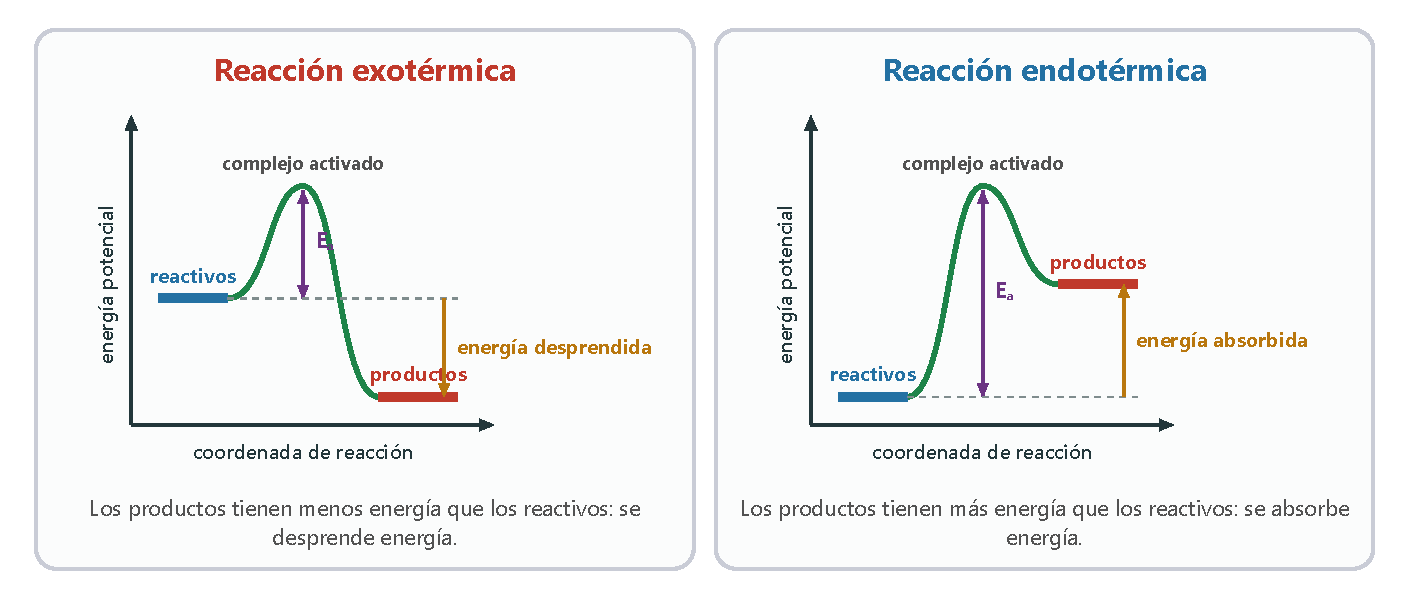
\includegraphics[width=0.85\textwidth]{images/UD6/exo_endo}
    \caption{Diagramas entálpicos de una reacción exotérmica (\(\Delta H < 0\)) y de una endotérmica (\(\Delta H > 0\)).}
    \label{fig:ud6-exo-endo}
\end{figure}

Los \textbf{diagramas entálpicos} (figura~\ref{fig:ud6-exo-endo}) representan la energía del sistema a medida que avanza la
reacción. Fíjate en que todas las reacciones, también las exotérmicas, necesitan un aporte inicial de energía, la \textbf{energía
de activación}, para empezar: por eso hay que encender una vela con una cerilla, aunque después la combustión se mantenga sola.

Algunos productos aprovechan estos intercambios: las \textbf{bolsas de frío instantáneo} contienen una sal, como el nitrato de
amonio, cuya disolución en agua es endotérmica, y los \textbf{envases autocalentables} usan la reacción exotérmica del óxido de
calcio con el agua, \ch{CaO(s) + H2O(l) -> Ca(OH)2(s)}.

\subsection{Ecuaciones termoquímicas}

\begin{definition}[Ecuación termoquímica]
    Es una ecuación química ajustada que incluye el \textbf{estado físico} de todas las sustancias y la \textbf{variación de
    entalpía} de la reacción. Por ejemplo:
    \[ \ch{2 H2(g) + O2(g) -> 2 H2O(g)} \qquad \Delta H = \qty{-483.6}{\kilo\joule} \]
    indica que en la formación de 2 mol de vapor de agua se desprenden \qty{483.6}{\kilo\joule}.
\end{definition}

De ella se deduce que:
\begin{itemize}
    \item El proceso inverso es endotérmico y absorbe la misma energía: \ch{2 H2O(g) -> 2 H2(g) + O2(g)},
    \(\Delta H = \qty{+483.6}{\kilo\joule}\).
    \item Como la entalpía es extensiva, al formar 1 mol de \ch{H2O(g)} se desprende la mitad, \qty{241.8}{\kilo\joule}: si se
    multiplica la ecuación por un número, \(\Delta H\) se multiplica por el mismo número. Por eso en las ecuaciones termoquímicas
    se admiten coeficientes fraccionarios.
    \item \(\Delta H\) depende del estado físico (no es lo mismo formar agua líquida que vapor) y de la presión y la temperatura. Se
    llama \textbf{entalpía estándar}, \(\Delta H^\circ\), la de una reacción a \qty{1}{\bar} (aproximadamente \qty{1}{\atm}) y,
    normalmente, \qty{25}{\degreeCelsius}.
\end{itemize}

\begin{exercise}
    Con la ecuación termoquímica anterior, ¿qué energía se desprende al quemar \qty{10}{\gram} de hidrógeno para dar vapor de agua?
    \begin{solu}
        \textcolor{blue}{\(n(\ch{H2}) = 10/2 = \qty{5}{\mol}\); por cada 2 mol se desprenden \qty{483.6}{\kilo\joule}.}
        \(5 \cdot \dfrac{\num{483.6}}{2} = \textcolor{red}{\qty{1209}{\kilo\joule}}\) desprendidos.
    \end{solu}
\end{exercise}

\subsection{Medida experimental de la entalpía: el calorímetro}

Para medir el calor de reacción se lleva a cabo la reacción dentro de un \textbf{calorímetro}: un recipiente aislado que contiene
una masa conocida de agua (figura~\ref{fig:ud6-calorimetro}). Como sus paredes no dejan pasar el calor, todo el que desprende o
absorbe la reacción lo gana o lo pierde el agua, cuya temperatura cambia. Midiendo esa variación de temperatura:
\[ \Delta H = Q_p = -Q_{\text{agua}} = -m_{\text{agua}} \cdot c_{\text{agua}} \cdot \Delta T \qquad
c_{\text{agua}} = \qty{4.18}{\joule\per\gram\per\degreeCelsius} \]
Para medidas precisas hay que tener en cuenta también el calor que absorben las piezas del calorímetro.

\begin{figure}[H]
    \centering
    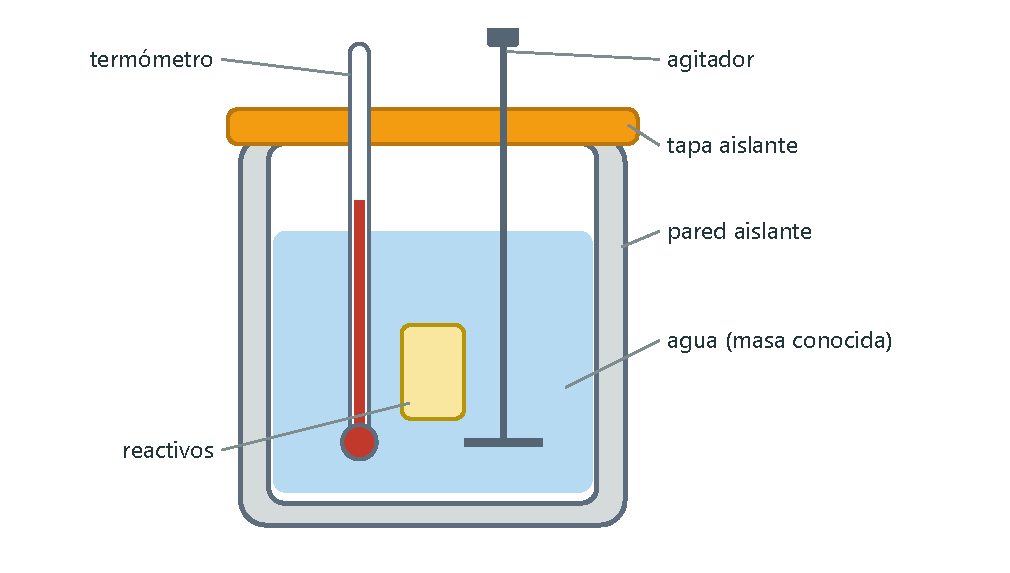
\includegraphics[width=0.5\textwidth]{images/UD6/calorimetro}
    \caption{Calorímetro: el calor de la reacción se mide por la variación de temperatura del agua.}
    \label{fig:ud6-calorimetro}
\end{figure}

\begin{exercise}
    En un calorímetro se mezclan \qty{100}{\mL} de \ch{HCl} \qty{1}{\mol\per\litre} con \qty{100}{\mL} de \ch{NaOH}
    \qty{1}{\mol\per\litre}, y la temperatura sube \qty{6.7}{\degreeCelsius}. Calcula la entalpía de neutralización por mol de
    agua formada. Supón que la mezcla tiene la densidad y el calor específico del agua.
    \begin{solu}
        \textcolor{blue}{\(Q_{\text{agua}} = 200 \cdot \num{4.18} \cdot \num{6.7} = \qty{5601}{\joule}\); se forman
        \(\num{0.1}\) mol de agua.} \(\Delta H = -\dfrac{\qty{5.60}{\kilo\joule}}{\qty{0.1}{\mol}} =
        \textcolor{red}{\qty{-56.0}{\kilo\joule\per\mol}}\).
    \end{solu}
\end{exercise}

\subsection{Ley de Hess}

Hay reacciones cuya entalpía no se puede medir directamente. Como la entalpía es una función de estado, se puede calcular
combinando otras reacciones conocidas:

\begin{definition}[Ley de Hess]
    La variación de entalpía de una reacción es la misma tanto si se produce en una sola etapa como en varias. Si una ecuación se
    puede obtener sumando otras (multiplicadas o invertidas si hace falta), su \(\Delta H\) se obtiene haciendo las mismas
    operaciones con sus entalpías.
\end{definition}

Por ejemplo, la combustión del carbono da el mismo calor si se produce directamente o pasando por monóxido de carbono
(figura~\ref{fig:ud6-hess}): \(\num{-110.5} + (\num{-283.0}) = \qty{-393.5}{\kilo\joule}\).

\begin{figure}[H]
    \centering
    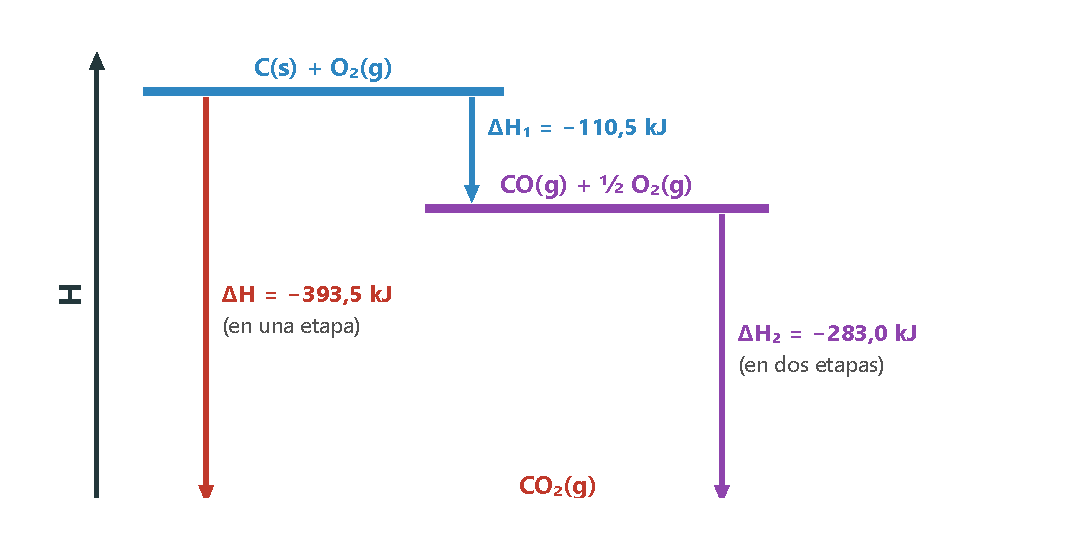
\includegraphics[width=0.6\textwidth]{images/UD6/hess}
    \caption{Ley de Hess: la entalpía de combustión del carbono no depende del camino.}
    \label{fig:ud6-hess}
\end{figure}

\begin{example}
    \textbf{Entalpía de formación del acetileno.} Con estos datos, calcula \(\Delta H\) para \ch{2 C(grafito) + H2(g) ->
    C2H2(g)}:
    \[ \begin{aligned}
        &\text{(A)}\ \ \ch{C(grafito) + O2(g) -> CO2(g)} && \Delta H_A = \qty{-393.5}{\kilo\joule} \\
        &\text{(B)}\ \ \ch{H2(g) + 1/2 O2(g) -> H2O(l)} && \Delta H_B = \qty{-285.8}{\kilo\joule} \\
        &\text{(C)}\ \ \ch{2 C2H2(g) + 5 O2(g) -> 4 CO2(g) + 2 H2O(l)} && \Delta H_C = \qty{-2599.2}{\kilo\joule}
    \end{aligned} \]

    \textbf{Solución.} Necesitamos 2 C a la izquierda (multiplicamos A por 2), 1 \ch{H2} a la izquierda (B tal cual) y 1 \ch{C2H2} a
    la derecha (invertimos C y la dividimos entre 2):
    \[ \begin{aligned}
        &\ch{2 C(grafito) + 2 O2 -> 2 CO2} && 2 \cdot (\num{-393.5}) = \qty{-787.0}{\kilo\joule} \\
        &\ch{H2 + 1/2 O2 -> H2O} && \qty{-285.8}{\kilo\joule} \\
        &\ch{2 CO2 + H2O -> C2H2 + 5/2 O2} && -\tfrac{1}{2} \cdot (\num{-2599.2}) = \qty{+1299.6}{\kilo\joule}
    \end{aligned} \]
    Al sumar, se cancelan el \ch{CO2}, el \ch{H2O} y el \ch{O2}: \ch{2 C(grafito) + H2 -> C2H2},
    \(\Delta H = -787{,}0 - 285{,}8 + 1299{,}6 = \qty{226.8}{\kilo\joule}\). Es endotérmica.
\end{example}

\begin{exercise}
    Con las entalpías de combustión del C(grafito) (\qty{-393.5}{\kilo\joule\per\mol}), del \ch{H2(g)}
    (\qty{-285.8}{\kilo\joule\per\mol}, dando agua líquida) y del \ch{CH4(g)} (\qty{-890.3}{\kilo\joule\per\mol}), calcula la
    entalpía de la reacción \ch{C(grafito) + 2 H2(g) -> CH4(g)}.
    \begin{solu}
        \textcolor{blue}{(A) + 2\(\cdot\)(B) \(-\) (C): \(\Delta H = -393{,}5 + 2 \cdot (-285{,}8) + 890{,}3\).}
        \(\Delta H = \textcolor{red}{\qty{-74.8}{\kilo\joule}}\).
    \end{solu}
\end{exercise}

\begin{exercise}
    Calcula la entalpía de oxidación del zinc, \ch{Zn(s) + 1/2 O2(g) -> ZnO(s)}, a partir de:
    \ch{Zn(s) + H2SO4(aq) -> ZnSO4(aq) + H2(g)}, \(\Delta H_A = \qty{-335}{\kilo\joule}\);
    \ch{2 H2(g) + O2(g) -> 2 H2O(l)}, \(\Delta H_B = \qty{-571.6}{\kilo\joule}\);
    \ch{ZnO(s) + H2SO4(aq) -> ZnSO4(aq) + H2O(l)}, \(\Delta H_C = \qty{-215}{\kilo\joule}\).
    \begin{solu}
        \textcolor{blue}{A + \(\frac{1}{2}\)B \(-\) C: \(\Delta H = -335 + \frac{1}{2}(-571{,}6) - (-215)\).}
        \(\Delta H = \textcolor{red}{\qty{-405.8}{\kilo\joule}}\).
    \end{solu}
\end{exercise}

\subsection{Entalpía de formación}

La entalpía de una reacción depende del estado físico de reactivos y productos. Por convenio, se toma como \textbf{estado estándar}
de una sustancia su forma más estable a \qty{1}{\bar} y \qty{25}{\degreeCelsius}.

\begin{definition}[Entalpía estándar de formación]
    La entalpía estándar de formación de un compuesto, \(\Delta H_f^\circ\), es la variación de entalpía de la reacción en la que se
    forma \textbf{un mol} del compuesto, en estado estándar, a partir de sus \textbf{elementos} en estado estándar. Por convenio, la
    de los elementos en su forma más estable (\ch{O2(g)}, \ch{N2(g)}, C(grafito), Fe(s), Hg(l)…) es \textbf{cero}.
\end{definition}

Aplicando la ley de Hess, la entalpía estándar de cualquier reacción se calcula a partir de las entalpías de formación tabuladas:
\[ \Delta H^\circ = \sum n_p\, \Delta H_f^\circ(\text{productos}) - \sum n_r\, \Delta H_f^\circ(\text{reactivos}) \]
donde \(n_p\) y \(n_r\) son los coeficientes de la ecuación ajustada: hacen falta porque los valores de la tabla son por mol.

\begin{table}[H]
    \centering
    \caption{Entalpías estándar de formación a \qty{25}{\degreeCelsius}}
    \vspace{-5pt}
    \begin{tabular}{@{}lr@{\hspace{1.5cm}}lr@{\hspace{1.5cm}}lr@{}}
        \toprule
        \textbf{Sustancia} & \makecell{\(\Delta H_f^\circ\)\\(\unit{\kilo\joule\per\mol})} &
        \textbf{Sustancia} & \makecell{\(\Delta H_f^\circ\)\\(\unit{\kilo\joule\per\mol})} &
        \textbf{Sustancia} & \makecell{\(\Delta H_f^\circ\)\\(\unit{\kilo\joule\per\mol})} \\
        \midrule
        \ch{H2O(g)} & \(-241{,}8\) & \ch{NO(g)} & \(90{,}3\) & \ch{CH4(g)} & \(-74{,}8\) \\[3pt]
        \ch{H2O(l)} & \(-285{,}8\) & \ch{NO2(g)} & \(33{,}2\) & \ch{C2H2(g)} & \(226{,}7\) \\[3pt]
        \ch{CO(g)} & \(-110{,}5\) & \ch{NH3(g)} & \(-46{,}2\) & \ch{C3H8(g)} & \(-103{,}8\) \\[3pt]
        \ch{CO2(g)} & \(-393{,}5\) & \ch{HCl(g)} & \(-92{,}3\) & \ch{C2H5OH(l)} & \(-277{,}7\) \\[3pt]
        \ch{SO2(g)} & \(-296{,}8\) & \ch{H2S(g)} & \(-20{,}6\) & \ch{CaCO3(s)} & \(-1206{,}9\) \\[3pt]
        \ch{SO3(g)} & \(-395{,}7\) & \ch{HNO3(l)} & \(-174{,}1\) & \ch{CaO(s)} & \(-635{,}1\) \\
        \bottomrule
    \end{tabular}
    \label{tab:ud6-formacion}
\end{table}

\begin{example}
    \textbf{Combustión del metano.} Con la tabla~\ref{tab:ud6-formacion}, calcula la entalpía de combustión del metano para dar
    \ch{CO2(g)} y \ch{H2O(l)}.

    \textbf{Solución.} \ch{CH4(g) + 2 O2(g) -> CO2(g) + 2 H2O(l)}.
    \[ \Delta H^\circ = \big[(-393{,}5) + 2 \cdot (-285{,}8)\big] - \big[(-74{,}8) + 2 \cdot 0\big] = \qty{-890.3}{\kilo\joule} \]
\end{example}

\begin{exercise}
    Calcula, con la tabla~\ref{tab:ud6-formacion}, la entalpía de combustión del etanol, \ch{C2H5OH(l)}, para dar \ch{CO2(g)} y
    \ch{H2O(l)}.
    \begin{solu}
        \textcolor{blue}{\ch{C2H5OH + 3 O2 -> 2 CO2 + 3 H2O}; \(\Delta H^\circ = 2(-393{,}5) + 3(-285{,}8) - (-277{,}7)\).}
        \(\Delta H^\circ = \textcolor{red}{\qty{-1366.7}{\kilo\joule\per\mol}}\).
    \end{solu}
\end{exercise}

\begin{exercise}
    Calcula la entalpía de combustión del acetileno, \ch{C2H2(g)}, con agua líquida como producto. ¿Qué energía se desprende al
    quemar \qty{1}{\kilo\gram} de acetileno?
    \begin{solu}
        \textcolor{blue}{\ch{C2H2 + 5/2 O2 -> 2 CO2 + H2O}; \(\Delta H^\circ = 2(-393{,}5) + (-285{,}8) - 226{,}7\).}
        \(\Delta H^\circ = \textcolor{red}{\qty{-1299.5}{\kilo\joule\per\mol}}\); \(n = 1000/26 = \qty{38.5}{\mol}\):
        \textcolor{red}{\qty{5.0e4}{\kilo\joule}} desprendidos.
    \end{solu}
\end{exercise}

\subsection{Entalpía de combustión}

\begin{definition}[Entalpía estándar de combustión]
    Es la variación de entalpía, \(\Delta H_c^\circ\), de la reacción en la que \textbf{un mol} de una sustancia reacciona
    completamente con oxígeno, con reactivos y productos en estado estándar.
\end{definition}

Es siempre negativa y mide el poder energético de un combustible. Con la ley de Hess, igual que con las de formación, se pueden
calcular entalpías de reacción a partir de entalpías de combustión tabuladas (fíjate en que la fórmula se invierte):
\[ \Delta H^\circ = \sum n_r\, \Delta H_c^\circ(\text{reactivos}) - \sum n_p\, \Delta H_c^\circ(\text{productos}) \]

\subsection{Entalpía de enlace}

\begin{definition}[Entalpía de enlace]
    Es la energía necesaria para romper un mol de enlaces entre dos átomos de una sustancia en estado gaseoso. Siempre es positiva.
\end{definition}

La entalpía de una reacción es, de forma aproximada, la diferencia entre la energía que se invierte en romper los enlaces de los
reactivos y la que se desprende al formar los de los productos:
\[ \Delta H^\circ \approx \sum \Delta H_{\text{enlaces rotos}} - \sum \Delta H_{\text{enlaces formados}} \]
El resultado es aproximado porque los valores tabulados son medias de los de muchas sustancias.

\begin{table}[H]
    \centering
    \caption{Entalpías medias de enlace (\unit{\kilo\joule\per\mol})}
    \vspace{-5pt}
    \begin{tabular}{@{}lr@{\hspace{1.2cm}}lr@{\hspace{1.2cm}}lr@{\hspace{1.2cm}}lr@{}}
        \toprule
        \textbf{Enlace} & \textbf{\(\Delta H\)} & \textbf{Enlace} & \textbf{\(\Delta H\)} & \textbf{Enlace} &
        \textbf{\(\Delta H\)} & \textbf{Enlace} & \textbf{\(\Delta H\)} \\
        \midrule
        H--H & 436 & C--H & 414 & C--C & 347 & N\(\equiv\)N & 945 \\[3pt]
        Cl--Cl & 243 & C--Cl & 339 & C=C & 614 & N--H & 391 \\[3pt]
        Br--Br & 193 & H--Cl & 432 & C=O & 745 & O=O & 498 \\[3pt]
        I--I & 151 & H--Br & 366 & C--O & 358 & O--H & 463 \\
        \bottomrule
    \end{tabular}
    \label{tab:ud6-enlace}
\end{table}

\begin{example}
    \textbf{Bromuro de hidrógeno.} Calcula la entalpía de formación del bromuro de hidrógeno gaseoso a partir de las entalpías de
    enlace.

    \textbf{Solución.} \ch{H2(g) + Br2(g) -> 2 HBr(g)}. Se rompen un enlace H--H y uno Br--Br, y se forman dos H--Br:
    \[ \Delta H = (436 + 193) - 2 \cdot 366 = \qty{-103}{\kilo\joule} \]
    Esto corresponde a 2 mol de \ch{HBr}: \(\Delta H_f \approx \qty{-51.5}{\kilo\joule\per\mol}\).
\end{example}

\begin{exercise}
    Calcula con las entalpías de enlace: a) la entalpía de formación del \ch{HCl(g)}; b) la entalpía de la reacción
    \ch{CH4(g) + Cl2(g) -> CH3Cl(g) + HCl(g)}.
    \begin{solu}
        a) \textcolor{blue}{\ch{H2 + Cl2 -> 2 HCl}: \(436 + 243 - 2 \cdot 432 = \qty{-185}{\kilo\joule}\) por 2 mol.}
        \textcolor{red}{\(\Delta H_f \approx \qty{-92.5}{\kilo\joule\per\mol}\)} (el valor tabulado es \(-92{,}3\)).
        b) \textcolor{blue}{Se rompen un C--H y un Cl--Cl; se forman un C--Cl y un H--Cl.} \(\Delta H = (414 + 243) - (339 + 432) =
        \textcolor{red}{\qty{-114}{\kilo\joule}}\).
    \end{solu}
\end{exercise}

%========================================================================================
\section{Combustiones}\label{sec:ud6-combustiones}
%========================================================================================

Las \textbf{combustiones} son reacciones redox en las que una sustancia, el \textbf{combustible}, reacciona con otra, el
\textbf{comburente} (normalmente el oxígeno del aire), desprendiendo energía. Su velocidad es muy variada: desde las lentísimas,
como la respiración celular, que «quema» la glucosa, hasta las explosiones.

\paragraph{Combustibles fósiles.} Alrededor del 80\,\% de la energía que consume la humanidad para cocinar, calentarse, moverse o
producir electricidad procede de quemar \textbf{combustibles fósiles}: el \textbf{petróleo}, el \textbf{carbón} y el \textbf{gas
natural}. Se formaron hace millones de años por la descomposición de restos de seres vivos. Contienen sobre todo
\textbf{hidrocarburos}, que arden según:
\[ \text{hidrocarburo} + \text{oxígeno} \ch{->} \text{dióxido de carbono} + \text{agua} + \text{energía} \]
Por ejemplo, el metano del gas natural: \ch{CH4(g) + 2 O2(g) -> CO2(g) + 2 H2O(l)}, \(\Delta H = \qty{-890}{\kilo\joule}\).

Son baratos y relativamente fáciles de extraer, transportar y almacenar, pero su uso tiene graves inconvenientes:
\begin{itemize}
    \item El \ch{CO2} que se emite al quemarlos \textbf{intensifica el efecto invernadero} y provoca un calentamiento global con
    consecuencias como el deshielo de los polos, la subida del nivel del mar, los fenómenos meteorológicos extremos, la
    desertificación, los incendios, la pérdida de biodiversidad o las migraciones forzadas.
    \item Sus impurezas producen al quemarse \textbf{óxidos de azufre y de nitrógeno}, que con el agua de la atmósfera forman ácidos
    sulfúrico y nítrico: es la \textbf{lluvia ácida}, que daña la vegetación, acidifica suelos y acuíferos y corroe edificios y
    estructuras metálicas.
    \item Sus reservas son \textbf{limitadas}, generan \textbf{dependencia} de los países productores y su control es fuente de
    conflictos y tensiones geopolíticas: son \textbf{recursos estratégicos}.
\end{itemize}

\paragraph{El hidrógeno verde.} Una alternativa es el hidrógeno, cuya combustión solo produce agua:
\ch{2 H2(g) + O2(g) -> 2 H2O(l)}, \(\Delta H = \qty{-571.6}{\kilo\joule}\). El hidrógeno no se encuentra libre en la
naturaleza; puede obtenerse por \textbf{electrólisis} del agua, el proceso inverso, que necesita energía eléctrica. Si esa energía
procede de fuentes renovables, se habla de \textbf{hidrógeno verde}: es una forma de \textbf{almacenar} la energía del sol o del
viento para usarla después, por ejemplo en pilas de combustible.

\begin{exercise}
    La entalpía de combustión del butano es \qty{-2878}{\kilo\joule\per\mol}. a) ¿Qué energía se obtiene al quemar el contenido de
    una bombona de \qty{12.5}{\kilo\gram}? b) ¿Qué masa de \ch{CO2} se emite?
    \begin{solu}
        a) \textcolor{blue}{\(n = 12500/58 = \qty{215.5}{\mol}\).} \(E = \num{215.5} \cdot 2878 = \textcolor{red}{\qty{6.20e5}{\kilo\joule}}\).
        b) \textcolor{blue}{\ch{C4H10 + 13/2 O2 -> 4 CO2 + 5 H2O}: \(4 \cdot \num{215.5} = \qty{862}{\mol}\) de \ch{CO2}.}
        \(862 \cdot 44 = \textcolor{red}{\qty{37.9}{\kilo\gram}}\) de \ch{CO2}.
    \end{solu}
\end{exercise}

\begin{exercise}
    Compara la energía que se obtiene al quemar \qty{1}{\gram} de hidrógeno (\(\Delta H_c = \qty{-285.8}{\kilo\joule\per\mol}\)) y
    \qty{1}{\gram} de octano, \ch{C8H18}, el principal componente de la gasolina (\(\Delta H_c = \qty{-5470}{\kilo\joule\per\mol}\)).
    ¿Qué ventajas e inconvenientes tiene el hidrógeno como combustible?
    \begin{solu}
        \textcolor{blue}{Hidrógeno: \(\num{285.8}/2 = \qty{142.9}{\kilo\joule\per\gram}\); octano: \(5470/114 = \qty{48.0}{\kilo\joule\per\gram}\).}
        \textcolor{red}{El hidrógeno da casi 3 veces más energía por gramo} y solo produce agua. \textcolor{red}{Inconvenientes}:
        hay que fabricarlo (gastando energía), es un gas muy poco denso, difícil de almacenar y transportar, y es inflamable y
        explosivo.
    \end{solu}
\end{exercise}

\begin{exercise}
    Los tubos de escape de los coches llevan un \textbf{catalizador} que transforma los gases más nocivos. Investiga qué reacciones
    se producen en él y qué ventajas e inconvenientes tienen los biocombustibles como alternativa a la gasolina y el gasóleo.
    \begin{solu}
        \textcolor{red}{Respuesta abierta.} El catalizador (de platino, paladio y rodio) oxida el \ch{CO} y los hidrocarburos sin
        quemar a \ch{CO2} y agua (\ch{2 CO + O2 -> 2 CO2}) y reduce los óxidos de nitrógeno a \ch{N2}
        (\ch{2 NO + 2 CO -> N2 + 2 CO2}). Los biocombustibles (bioetanol, biodiésel) son renovables y su \ch{CO2} lo absorbieron
        antes las plantas, pero ocupan tierras de cultivo, encarecen los alimentos y pueden favorecer la deforestación.
    \end{solu}
\end{exercise}

%========================================================================================
\section{La industria química}\label{sec:ud6-industria}
%========================================================================================

\begin{definition}[Industria química]
    Es la que extrae y procesa \textbf{materias primas} (vegetales, animales, minerales, fuentes de energía, el agua y el aire) para
    transformarlas en \textbf{productos elaborados} que satisfacen necesidades de la sociedad y mejoran nuestra calidad de vida.
\end{definition}

Es tan antigua como la humanidad (la cerámica, los tintes, el jabón, la metalurgia), pero su gran desarrollo empezó con la
revolución industrial del siglo \textsc{xviii}. Se distinguen:
\begin{itemize}
    \item La \textbf{industria química de base}, que fabrica productos intermedios a partir de las materias primas: el ácido
    sulfúrico, el amoníaco o el etanol, por ejemplo.
    \item La \textbf{industria química de transformación}, que usa esos productos básicos para fabricar productos de \textbf{salud}
    (fármacos, productos fitosanitarios y veterinarios), de \textbf{consumo} (cosméticos, pinturas, detergentes, tejidos,
    plásticos) o para \textbf{otras industrias} (combustibles, explosivos, fertilizantes).
\end{itemize}

Un proceso industrial tiene que ser \textbf{rentable}, buscando el equilibrio entre rendimiento y costes, y a la vez
\textbf{respetuoso con el medio ambiente}. Muchas veces trabaja a presiones y temperaturas elevadas y en \textbf{flujo continuo}:
los reactivos entran y los productos salen del reactor sin parar. La \textbf{ingeniería química} diseña y optimiza estos procesos,
pasando de la investigación en el laboratorio a la producción a gran escala por medio de una \textbf{planta piloto}.

\subsection{La síntesis del amoníaco: el proceso Haber-Bosch}

El amoníaco es, tras el ácido sulfúrico, el producto químico que más se fabrica en el mundo: unos 200 millones de toneladas al
año, de las que el 85\,\% se destina a \textbf{fertilizantes}, imprescindibles para alimentar a la población mundial. También se
usa para fabricar explosivos, plásticos, productos de limpieza y como refrigerante.

En 1909, \textbf{Fritz Haber} consiguió sintetizarlo a partir del nitrógeno del aire, una reacción reversible y exotérmica:
\[ \ch{N2(g) + 3 H2(g) <=> 2 NH3(g)} \qquad \Delta H = \qty{-92.4}{\kilo\joule} \]
Ajustando la presión y la temperatura y usando un catalizador, optimizó el rendimiento y la velocidad. \textbf{Carl Bosch} lo
llevó a escala industrial gracias a la tecnología de alta presión. Los dos recibieron el premio Nobel.

\begin{figure}[H]
    \centering
    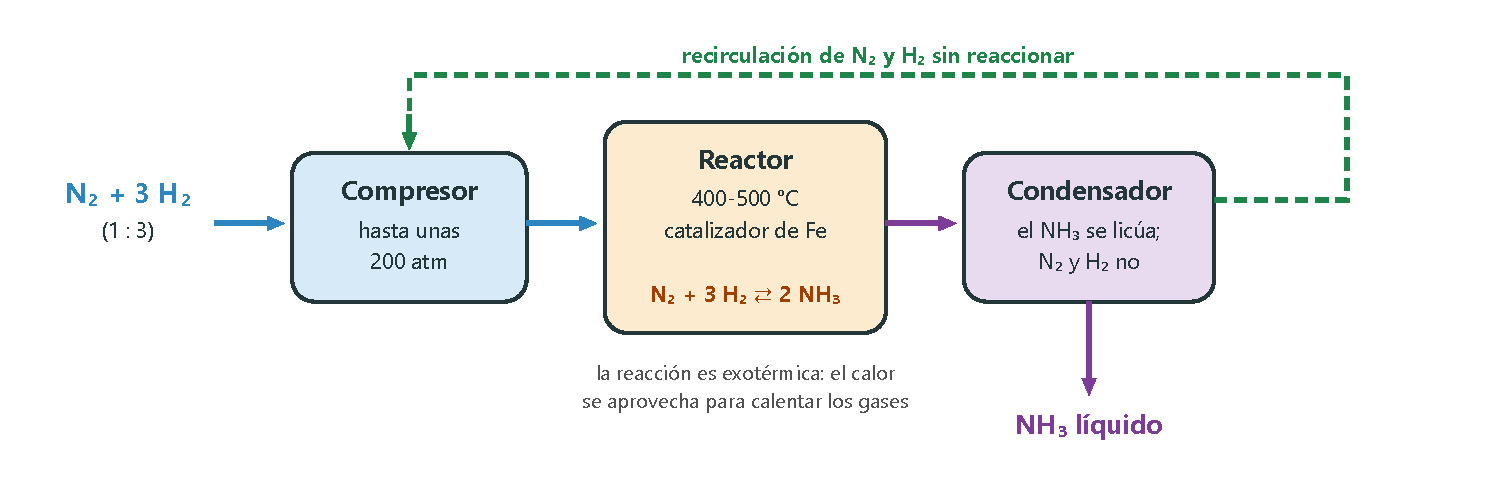
\includegraphics[width=0.85\textwidth]{images/UD6/haber_bosch}
    \caption{Esquema simplificado del proceso Haber-Bosch.}
    \label{fig:ud6-haber}
\end{figure}

\begin{exercise}
    En una planta de amoníaco se hacen reaccionar \qty{150}{\gram} de nitrógeno con \qty{30}{\gram} de hidrógeno. ¿Qué masa de
    amoníaco se obtiene si el rendimiento es del 60\,\%?
    \begin{solu}
        \textcolor{blue}{\(n(\ch{N2}) = 150/28 = \qty{5.36}{\mol}\), que necesitarían \qty{16.1}{\mol} de \ch{H2}; solo hay
        \(30/2 = \qty{15}{\mol}\): el \ch{H2} es el limitante. \(n(\ch{NH3}) = 15 \cdot \frac{2}{3} = \qty{10}{\mol}\) (\qty{170}{\gram}).}
        \(170 \cdot \num{0.60} = \textcolor{red}{\qty{102}{\gram}}\) de \ch{NH3}.
    \end{solu}
\end{exercise}

\begin{exercise}
    ¿Qué masa de amoníaco se obtiene, con un rendimiento del 60\,\%, si se mezclan \qty{3}{\litre} de \ch{H2} a \qty{2}{\atm} y
    \qty{4}{\litre} de \ch{N2} a \qty{1.8}{\atm}, ambos a \qty{25}{\degreeCelsius}?
    \begin{solu}
        \textcolor{blue}{\(n(\ch{H2}) = \dfrac{2 \cdot 3}{\num{0.082} \cdot 298} = \qty{0.246}{\mol}\);
        \(n(\ch{N2}) = \dfrac{\num{1.8} \cdot 4}{\num{0.082} \cdot 298} = \qty{0.295}{\mol}\). El \ch{H2} es el limitante (solo
        reacciona con \qty{0.082}{\mol} de \ch{N2}). \(n(\ch{NH3}) = \num{0.246} \cdot \frac{2}{3} = \qty{0.164}{\mol}\) (\qty{2.78}{\gram}).}
        \(\num{2.78} \cdot \num{0.60} = \textcolor{red}{\qty{1.67}{\gram}}\) de \ch{NH3}.
    \end{solu}
\end{exercise}

\subsection{La industria farmacéutica}

Desde la Antigüedad se han usado plantas para aliviar enfermedades: la adormidera como calmante, la manzanilla para el estómago…
A principios del siglo \textsc{xix}, con disolventes como el éter o el cloroformo, se aislaron los \textbf{principios activos} de
muchas de ellas, como la morfina o la cafeína, y en 1828 \textbf{Friedrich Wöhler} sintetizó en el laboratorio una sustancia
orgánica, la urea, a partir de compuestos inorgánicos. La \textbf{farmacología}, que estudia la composición, las propiedades y la
acción de los medicamentos, es una ciencia independiente desde mediados del siglo \textsc{xix}.

Desde que empieza la investigación hasta que un medicamento llega a la farmacia pueden pasar más de diez años:
\begin{enumerate}
    \item \textbf{Investigación y diseño}: se identifica la \textbf{diana} (normalmente una proteína relacionada con la enfermedad) y
    se busca un \textbf{principio activo} que actúe sobre ella. En la fase \textbf{preclínica} se estudia su seguridad y eficacia
    con modelos informáticos, en el laboratorio y en animales.
    \item \textbf{Ensayos clínicos}: se administra primero a un pequeño grupo de voluntarios sanos (fase I, seguridad y dosis),
    después a enfermos (fase II, eficacia) y finalmente en un estudio a gran escala (fase III).
    \item \textbf{Registro y comercialización}: las autoridades sanitarias evalúan los datos antes de autorizarlo. Una vez en el
    mercado, se sigue vigilando su seguridad (fase IV).
\end{enumerate}

\begin{remark}
    \textbf{Vacunas de ARN mensajero.} Las vacunas contra la COVID-19 se desarrollaron en un tiempo récord, pero gracias a décadas de
    investigación básica previa, como la de la bioquímica \textbf{Katalin Karikó} sobre el ARN mensajero, por la que recibió el
    premio Nobel en 2023. Como decía Ramón y Cajal: «Cultivemos la ciencia por sí misma, sin considerar por el momento las
    aplicaciones. Estas llegan siempre; a veces tardan años, a veces siglos».
\end{remark}

\subsection{Nuevos materiales}

La química, la física y la ingeniería de materiales desarrollan continuamente materiales con propiedades a la carta:
\begin{itemize}
    \item En \textbf{construcción}: madera translúcida, hormigón «autorreparable» con bacterias que sellan sus grietas o cementos
    que absorben luz de día y la emiten de noche.
    \item En \textbf{transporte}: espumas de aluminio, ligeras y resistentes a los impactos, o termoplásticos reciclables que
    aligeran coches y aviones y reducen su consumo.
    \item En \textbf{medicina}: prótesis de cerámica o de espuma de titanio, nanopartículas y liposomas que transportan fármacos
    hasta las células enfermas o materiales con memoria de forma.
    \item La \textbf{nanotecnología} manipula la materia átomo a átomo: a escala de nanómetros, los materiales presentan
    propiedades (resistencia, conductividad, reactividad) muy diferentes de las que tienen a mayor escala. El grafeno o los
    nanotubos de carbono son ejemplos.
\end{itemize}

\subsection{La química verde}

Durante mucho tiempo la industria química ha consumido grandes cantidades de recursos y ha emitido contaminantes al suelo, al aire
y al agua. La respuesta a este problema es la química verde.

\begin{definition}[Química verde o sostenible]
    Es una filosofía que busca diseñar productos y procesos químicos que reduzcan o eliminen el uso y la producción de sustancias
    peligrosas para la salud y el medio ambiente. Sus principios incluyen:
    \begin{itemize}
        \item \textbf{Prevenir} los residuos mejor que tratarlos después: procesos que incorporen al producto final todos los
        átomos de los reactivos (\textbf{economía atómica}).
        \item Usar y producir sustancias de \textbf{baja toxicidad} y minimizar el riesgo de accidentes.
        \item Ahorrar \textbf{energía} y usar fuentes y materias primas \textbf{renovables}.
        \item Usar \textbf{catalizadores} y diseñar productos \textbf{biodegradables}.
    \end{itemize}
\end{definition}

\begin{exercise}
    La economía atómica de un proceso es el porcentaje de la masa de los reactivos que acaba formando parte del producto deseado.
    Calcula la del proceso Haber-Bosch y la de la obtención de hidrógeno con zinc y ácido clorhídrico
    (\ch{Zn + 2 HCl -> ZnCl2 + H2}). ¿Cuál es más «verde» en este aspecto?
    \begin{solu}
        \textcolor{blue}{Haber-Bosch: todos los átomos acaban en el \ch{NH3}: \(\dfrac{34}{28 + 6} \cdot 100\).} \textcolor{red}{100\,\%}.
        \textcolor{blue}{Zinc: \(\dfrac{2}{\num{65.4} + 73} \cdot 100\).} \textcolor{red}{1,4\,\%}: casi toda la masa acaba en el
        subproducto, \ch{ZnCl2}. \textcolor{red}{El proceso Haber-Bosch es mucho más eficiente.}
    \end{solu}
\end{exercise}

\begin{exercise}
    Investiga sobre los diez medicamentos más vendidos en España: su principio activo, para qué se usan y alguna anécdota de su
    descubrimiento.
    \begin{solu}
        \textcolor{red}{Respuesta abierta.} Por ejemplo, el paracetamol y el ibuprofeno (analgésicos y antiinflamatorios), el
        omeprazol (protector gástrico), las estatinas (colesterol) o la amoxicilina (antibiótico, derivado de la penicilina
        descubierta por Fleming en 1928 al ver que un moho mataba sus cultivos de bacterias).
    \end{solu}
\end{exercise}

%========================================================================================
\section{Química en la vida: ¡al baño María!}\label{sec:ud6-bano}
%========================================================================================

Gracias a los programas de cocina, todo el mundo sabe lo que es cocinar al \textbf{baño María}: calentar un recipiente metiéndolo
en otro con agua caliente, en lugar de ponerlo directamente al fuego. El calor llega de forma lenta, suave y uniforme, y la
temperatura no pasa de \qty{100}{\degreeCelsius}, por lo que no se quema ni se altera lo que se calienta. Además de en la cocina, se
usa desde hace siglos en los laboratorios y en las industrias química, farmacéutica y cosmética.

Su origen nos lleva a la Alejandría del siglo \textsc{iii}, donde vivió \textbf{María la Judía}, una de las primeras alquimistas de
la historia, que lo utilizaba para destilar sustancias aromáticas y evaporar extractos. Sus obras se perdieron, quizá en el
incendio de la Biblioteca de Alejandría, pero las conocemos porque las citan otros autores, como su discípulo \textbf{Zósimo de
Panópolis}. Se le atribuyen también el \textit{tribikos}, un alambique de tres brazos para purificar sustancias por destilación, y
el \textit{kerotakis}, un aparato para extraer esencias de las plantas. Durante la Edad Media, muchos alquimistas usaron sus
técnicas en la búsqueda de la «quintaesencia», el supuesto quinto elemento, más puro que el agua, la tierra, el fuego y el aire.

Hoy sabemos que el agua es un medio excelente para calentar: tiene un \textbf{calor específico muy alto}
(\qty{4.18}{\joule\per\gram\per\degreeCelsius}) y, mientras hierve, su temperatura se mantiene constante.

\begin{exercise}
    a) ¿Por qué, al baño María, lo que se calienta no supera los \qty{100}{\degreeCelsius}? b) ¿Qué energía hace falta para calentar
    \qty{2}{\kilo\gram} de agua del baño de \qty{20}{\degreeCelsius} a \qty{90}{\degreeCelsius}? c) Elaborad en clase un
    \textbf{abecedario científico} con mujeres científicas destacadas de la historia; María la Judía puede ocupar la «J».
    \begin{solu}
        a) \textcolor{red}{Porque el agua líquida no puede superar su temperatura de ebullición} (a \qty{1}{\atm}): el calor
        adicional se emplea en evaporarla. b) \(Q = m\,c\,\Delta T = 2000 \cdot \num{4.18} \cdot 70 = \textcolor{red}{\qty{585}{\kilo\joule}}\).
        c) \textcolor{red}{Respuesta abierta}: por ejemplo, Hipatia, Marie Curie, Rosalind Franklin, Lise Meitner, Dorothy Hodgkin,
        Margarita Salas…
    \end{solu}
\end{exercise}

%========================================================================================
\section{Prácticas}\label{sec:ud6-practicas}
%========================================================================================

\subsection{Bicarbonato y vinagre: ¿quién es el reactivo limitante?}

\noindent\begin{minipage}[t]{0.48\textwidth}
    \textbf{Objetivo}
    \begin{itemize}
        \item Comprobar experimentalmente el concepto de reactivo limitante con la reacción del bicarbonato de sodio y el ácido
        acético del vinagre.
    \end{itemize}
\end{minipage}\hfill
\begin{minipage}[t]{0.48\textwidth}
    \textbf{Material y reactivos}
    \begin{itemize}
        \item Cinco botellas pequeñas de plástico iguales, cinco globos, embudo, probeta, balanza y cucharilla.
        \item Bicarbonato de sodio (\ch{NaHCO3}) y vinagre (ácido acético al 5\,\% en masa, \(d \approx \qty{1}{\gram\per\mL}\)).
    \end{itemize}
\end{minipage}

\textbf{Procedimiento}
\begin{enumerate}[label=\numberballgreen]
    \item Echa en cada botella \qty{50}{\mL} de vinagre.
    \item Con el embudo, pon en cada globo una cantidad distinta de bicarbonato: 1, 2, 3, 4 y \qty{6}{\gram}.
    \item Ajusta la boca de cada globo a una botella sin dejar caer el bicarbonato. Después, levanta los globos a la vez para que el
    bicarbonato caiga en el vinagre.
    \item Cuando acabe el burbujeo, compara el tamaño de los globos y observa si queda bicarbonato sin reaccionar en el fondo.
\end{enumerate}
\textbf{Trabaja con gafas.} La reacción es: \ch{NaHCO3(s) + CH3COOH(aq) -> CH3COONa(aq) + H2O(l) + CO2(g) ^}.

\begin{exercise}
    a) Calcula los moles de ácido acético que hay en \qty{50}{\mL} de vinagre y la masa de bicarbonato que reacciona exactamente con
    ellos. b) ¿En qué globos es limitante el bicarbonato y en cuáles el ácido? ¿Qué observarás? c) ¿Qué volumen de \ch{CO2} se
    obtiene como máximo a \qty{20}{\degreeCelsius} y \qty{1}{\atm}?
    \begin{solu}
        a) \textcolor{blue}{\(m(\text{ácido}) = 50 \cdot \num{0.05} = \qty{2.5}{\gram}\); \(n = \num{2.5}/60 = \qty{0.0417}{\mol}\).}
        \(m(\ch{NaHCO3}) = \num{0.0417} \cdot 84 = \textcolor{red}{\qty{3.5}{\gram}}\). b) \textcolor{red}{Con 1, 2 y \qty{3}{\gram}
        el limitante es el bicarbonato}: los globos crecen cada vez más y no sobra sólido. \textcolor{red}{Con 4 y \qty{6}{\gram}, el
        ácido}: los dos globos se inflan igual (el máximo) y queda bicarbonato en el fondo. c) \(V = \dfrac{\num{0.0417} \cdot
        \num{0.082} \cdot 293}{1} = \textcolor{red}{\qty{1.0}{\litre}}\).
    \end{solu}
\end{exercise}

\subsection{Química en la cocina: falso caviar de cacao}

\noindent\begin{minipage}[t]{0.48\textwidth}
    \textbf{Objetivo}
    \begin{itemize}
        \item Experimentar con una técnica de «cocina molecular», la gelificación en aceite frío, para obtener perlas parecidas al
        caviar.
    \end{itemize}
\end{minipage}\hfill
\begin{minipage}[t]{0.48\textwidth}
    \textbf{Material}
    \begin{itemize}
        \item \qty{30}{\gram} de cacao en polvo, \qty{50}{\gram} de azúcar, \qty{250}{\mL} de agua y \qty{2}{\gram} de agar-agar.
        \item Aceite de girasol, un vaso alto, un cazo, una jeringuilla grande y un colador.
    \end{itemize}
\end{minipage}

\textbf{Procedimiento}
\begin{enumerate}[label=\numberballgreen]
    \item Enfría el aceite en el vaso alto: en la nevera desde la noche anterior o media hora en el congelador. Debe estar a menos
    de \qty{4}{\degreeCelsius}.
    \item Mezcla en el cazo el cacao, el azúcar, el agua y el agar-agar y llévalo a ebullición, removiendo suavemente para no meter
    aire.
    \item Deja templar la mezcla al baño María (sin que llegue a cuajar) y carga la jeringuilla.
    \item Deja caer gotas en el aceite frío: al bajar, se enfrían y se convierten en perlas de gel que se depositan en el fondo.
    \item Cuela las perlas y acláralas con agua para quitarles el aceite.
\end{enumerate}
\textbf{Truco}: se puede sustituir el cacao por zumo de naranja, granadina o té matcha.

\begin{exercise}
    a) El agar-agar se disuelve en caliente (hacia \qty{90}{\degreeCelsius}) y gelifica al enfriarse (hacia \qty{40}{\degreeCelsius}),
    y el proceso se puede repetir. ¿Es un cambio químico o físico? b) ¿Por qué se usa aceite y no agua fría? c) Investiga qué es la
    esferificación con alginato y calcio, otra técnica de cocina molecular, y si es un proceso físico o químico.
    \begin{solu}
        a) \textcolor{red}{Físico}: es reversible y las moléculas del agar no cambian; solo forman una red que atrapa el agua al
        enfriarse. b) \textcolor{red}{Porque la mezcla es acuosa y no se mezcla con el aceite}: cada gota conserva su forma
        esférica mientras gelifica; en agua se disolvería. c) \textcolor{red}{Respuesta abierta}: el alginato de sodio (extraído
        de algas pardas) reacciona con los iones \ch{Ca^2+} y forma una membrana de alginato de calcio insoluble alrededor de la
        gota: es una \textcolor{red}{reacción química} (un intercambio de iones).
    \end{solu}
\end{exercise}

%========================================================================================
\section{Situación de aprendizaje: química verde (ODS 7, 12 y 13)}\label{sec:ud6-ods}
%========================================================================================

La industria química transforma materias primas en productos que mejoran nuestra vida y genera empleo y riqueza. Pero los
productos químicos liberados al medio ambiente han causado pérdida de biodiversidad, contaminación de aguas y suelos, el deterioro
de la capa de ozono o el aumento del efecto invernadero, además de consumir muchos recursos no renovables. La \textbf{química verde},
cuyas bases establecieron \textbf{Paul Anastas} y \textbf{John Warner} en 1998 con sus «doce principios», propone diseñar los
productos y los procesos para prevenir la contaminación desde el origen, durante todo su ciclo de vida.

Los \textbf{Objetivos de Desarrollo Sostenible 7} (energía asequible y no contaminante), \textbf{12} (producción y consumo
responsables) y \textbf{13} (acción por el clima) están muy relacionados con la industria química. La Unión Europea, a través del
\textbf{Pacto Verde Europeo}, se ha propuesto ser climáticamente neutra en 2050.

\begin{marker}
    \textbf{Reto:} elaborad un mural (físico o digital) con propuestas de la química verde que os parezcan más interesantes para
    reducir el impacto ambiental de la industria química, explicando a qué principios responden.
\end{marker}

\begin{enumerate}[label=\numberballred]
    \item \textbf{Investigad} los doce principios de la química verde y la trayectoria de sus «padres fundadores». Elegid un producto
    químico cotidiano (un detergente, un plástico, un fármaco) y analizad qué principios cumple o podría cumplir.
    \item \textbf{Investigad} un proceso industrial clásico, la obtención del ácido nítrico por el \textbf{método Ostwald}, cuyas
    etapas son:
    \ch{NH3 + O2 -> NO + H2O}; \ch{NO + O2 -> NO2}; \ch{NO2 + H2O -> HNO3 + NO}. ¿Qué residuos genera? ¿Cómo se
    aprovecha el \ch{NO} de la última etapa?
    \item \textbf{Calculad.} Ajustad las tres reacciones del método Ostwald. Si se parte de \qty{1000}{\litre} de amoníaco medidos
    en condiciones normales y el rendimiento global es del 85\,\%, ¿qué masa de ácido nítrico del 60\,\% en masa se obtiene?
    (Supón que el \ch{NO} de la tercera etapa no se recicla.)
    \item \textbf{Comunicad.} El mural debe incluir: los doce principios ilustrados con ejemplos; el análisis del producto elegido;
    el proceso Ostwald con sus impactos y alguna mejora sostenible, y una propuesta de consumo responsable para el día a día
    (reducir, reutilizar y reciclar; alimentación y movilidad sostenibles).
\end{enumerate}

\begin{exercise}
    Resuelve los cálculos del apartado 3 de la situación de aprendizaje.
    \begin{solu}
        \textcolor{blue}{Ajustadas: \ch{4 NH3 + 5 O2 -> 4 NO + 6 H2O}; \ch{2 NO + O2 -> 2 NO2};
        \ch{3 NO2 + H2O -> 2 HNO3 + NO}. Cada mol de \ch{NH3} da 1 mol de \ch{NO} y 1 de \ch{NO2}, y cada 3 de \ch{NO2} dan 2 de
        \ch{HNO3}: \(n(\ch{NH3}) = 1000/\num{22.4} = \qty{44.6}{\mol}\); \(n(\ch{HNO3}) = \num{44.6} \cdot \frac{2}{3} \cdot
        \num{0.85} = \qty{25.3}{\mol}\), es decir, \(\num{25.3} \cdot 63 = \qty{1594}{\gram}\) de \ch{HNO3} puro.}
        \(\dfrac{1594}{\num{0.60}} = \textcolor{red}{\qty{2.66}{\kilo\gram}}\) de ácido del 60\,\%.
    \end{solu}
\end{exercise}

    \newpage
    %! Unidad 6 — Reacciones químicas: ejercicios resueltos y ejercicios finales
%! Fuente: Fuentes/Quimica/Unidad 6 («Ejercicios resueltos», «Practica y calcula», «Piensa y resuelve», «Situaciones de aprendizaje»).
%! Enunciados adaptados con sustancias y datos cambiados; soluciones rehechas. Dificultad: \(\star\) baja, \(\star\star\) media, \(\star\star\star\) alta.
%! Los ejercicios de termoquímica (no los trae la fuente al final) son nuevos.

\section{Ejercicios resueltos}\label{sec:ud6-resueltos}

Salvo que se indique otra cosa, usa las masas atómicas H = 1; C = 12; N = 14; O = 16; Na = 23; Mg = 24,3; Al = 27; S = 32;
Cl = 35,5; K = 39,1; Ca = 40; Fe = 55,8; Cu = 63,5; Zn = 65,4; \(R = \qty{0.082}{\atm\litre\per\mole\per\kelvin}\), y las tablas
\ref{tab:ud6-formacion} y \ref{tab:ud6-enlace}.

\begin{example}
    \textbf{Tostación de la blenda.} La blenda es un mineral de sulfuro de zinc, \ch{ZnS}, del que se obtiene el zinc. Al tostarla
    se produce la reacción \ch{2 ZnS(s) + 3 O2(g) -> 2 ZnO(s) + 2 SO2(g)}. Se tuestan \qty{1.5}{\kilo\gram} de un mineral con
    un 75\,\% de \ch{ZnS}. a) ¿Qué volumen de \ch{SO2} se obtiene, medido a \qty{900}{\mmHg} y \qty{500}{\degreeCelsius}? b) ¿Qué
    volumen de aire (21\,\% de \ch{O2} en volumen), medido en condiciones normales, se necesita?

    \textbf{Solución.} \textbf{1. Datos}: \(m = \qty{1500}{\gram}\) de mineral; riqueza 75\,\%; \(p = \qty{900}{\mmHg}\);
    \(T = \qty{773}{\kelvin}\); \(M(\ch{ZnS}) = \qty{97.4}{\gram\per\mol}\). \textbf{Incógnitas}: \(V(\ch{SO2})\) y \(V(\text{aire})\).

    \textbf{2. a)} Masa y moles de \ch{ZnS} puro, y moles de \ch{SO2} (proporción 2 : 2):
    \[ \qty{1500}{\gram}\ \text{mineral} \cdot \frac{\qty{75}{\gram}\ \ch{ZnS}}{\qty{100}{\gram}\ \text{mineral}} = \qty{1125}{\gram}\ \ch{ZnS}
    \ \rightarrow\ n = \frac{1125}{\num{97.4}} = \qty{11.55}{\mol}\ \ch{ZnS} = \qty{11.55}{\mol}\ \ch{SO2} \]
    \[ p = \frac{900}{760} = \qty{1.184}{\atm} \qquad V = \frac{n R T}{p} = \frac{\num{11.55} \cdot \num{0.082} \cdot 773}{\num{1.184}}
    = \qty{618}{\litre}\ \text{de}\ \ch{SO2} \]

    \textbf{3. b)} Moles de oxígeno (proporción 2 : 3) y su volumen en condiciones normales:
    \[ \qty{11.55}{\mol}\ \ch{ZnS} \cdot \frac{\qty{3}{\mol}\ \ch{O2}}{\qty{2}{\mol}\ \ch{ZnS}} = \qty{17.33}{\mol}\ \ch{O2}
    \ \rightarrow\ V = \num{17.33} \cdot \num{22.4} = \qty{388}{\litre}\ \ch{O2} \]
    \[ V(\text{aire}) = \qty{388}{\litre}\ \ch{O2} \cdot \frac{\qty{100}{\litre}\ \text{aire}}{\qty{21}{\litre}\ \ch{O2}} = \qty{1848}{\litre}\ \text{de aire} \]
\end{example}

\begin{example}
    \textbf{Reactivo limitante en disolución.} Se mezclan \qty{30}{\mL} de una disolución de hidróxido de potasio
    \qty{2}{\mol\per\litre} con \qty{6}{\mL} de ácido clorhídrico del 36\,\% en masa y densidad \qty{1.18}{\gram\per\mL}. Se forman
    cloruro de potasio y agua. Calcula la masa de \ch{KCl} y de agua que se forma y la cantidad de reactivo en exceso.

    \textbf{Solución.} \textbf{1. Ecuación}: \ch{KOH + HCl -> KCl + H2O} (proporción 1 : 1).

    \textbf{2. Moles de cada reactivo}:
    \[ n(\ch{KOH}) = \num{0.030} \cdot 2 = \qty{0.060}{\mol} \]
    \[ \qty{6}{\mL}\ \text{dis.} \cdot \frac{\qty{1.18}{\gram}\ \text{dis.}}{\qty{1}{\mL}} \cdot \frac{\qty{36}{\gram}\ \ch{HCl}}{\qty{100}{\gram}\ \text{dis.}}
    \cdot \frac{\qty{1}{\mol}}{\qty{36.5}{\gram}} = \qty{0.0698}{\mol}\ \ch{HCl} \]

    \textbf{3. Limitante}: como reaccionan mol a mol y hay menos \ch{KOH}, \textbf{el \ch{KOH} es el limitante}.

    \textbf{4. Productos y exceso}: \(m(\ch{KCl}) = \num{0.060} \cdot \num{74.6} = \qty{4.48}{\gram}\);
    \(m(\ch{H2O}) = \num{0.060} \cdot 18 = \qty{1.08}{\gram}\). Sobran \(\num{0.0698} - \num{0.060} = \qty{0.0098}{\mol}\) de \ch{HCl}
    (\qty{0.36}{\gram}).
\end{example}

\begin{example}
    \textbf{Ley de Hess y energía de un combustible.} a) Calcula la entalpía de formación del etanol, \ch{C2H5OH(l)}, sabiendo
    que las entalpías de combustión del C(grafito), del \ch{H2(g)} y del etanol son, respectivamente, \(-393{,}5\), \(-285{,}8\) y
    \qty{-1366.8}{\kilo\joule\per\mol} (el agua se forma líquida). b) ¿Qué energía se obtiene al quemar \qty{1}{\litre} de etanol
    (\(d = \qty{0.79}{\gram\per\mL}\))?

    \textbf{Solución.} a) Buscamos \ch{2 C(grafito) + 3 H2(g) + 1/2 O2(g) -> C2H5OH(l)}. Sumamos:
    \[ \begin{aligned}
        &\ch{2 C + 2 O2 -> 2 CO2} && 2 \cdot (\num{-393.5}) = \qty{-787.0}{\kilo\joule} \\
        &\ch{3 H2 + 3/2 O2 -> 3 H2O} && 3 \cdot (\num{-285.8}) = \qty{-857.4}{\kilo\joule} \\
        &\ch{2 CO2 + 3 H2O -> C2H5OH + 3 O2} && \qty{+1366.8}{\kilo\joule} \text{ (combustión invertida)}
    \end{aligned} \]
    \(\Delta H_f^\circ = -787{,}0 - 857{,}4 + 1366{,}8 = \qty{-277.6}{\kilo\joule\per\mol}\) (coincide con el de la tabla).

    b) \(m = 1000 \cdot \num{0.79} = \qty{790}{\gram}\); \(n = 790/46 = \qty{17.2}{\mol}\);
    \(E = \num{17.2} \cdot \num{1366.8} = \qty{2.35e4}{\kilo\joule}\) desprendidos.
\end{example}

\begin{example}
    \textbf{Entalpías de enlace.} Calcula, a partir de las entalpías de enlace, la entalpía de formación del amoníaco y compárala
    con el valor de la tabla~\ref{tab:ud6-formacion}. ¿Por qué no coinciden exactamente?

    \textbf{Solución.} \ch{N2(g) + 3 H2(g) -> 2 NH3(g)}. Se rompen un enlace \(\mathrm{N{\equiv}N}\) y tres H--H, y se forman
    seis N--H:
    \[ \Delta H = (945 + 3 \cdot 436) - 6 \cdot 391 = 2253 - 2346 = \qty{-93}{\kilo\joule} \]
    Corresponde a 2 mol de \ch{NH3}: \(\Delta H_f \approx \qty{-46.5}{\kilo\joule\per\mol}\), muy cerca del valor tabulado
    (\(-46{,}2\)). No coinciden exactamente porque las entalpías de enlace son \textbf{valores medios} de muchas moléculas distintas.
\end{example}

\begin{example}
    \textbf{Fermentación.} En la fabricación del vino, las levaduras transforman la glucosa del mosto en etanol y \ch{CO2}:
    \ch{C6H12O6 -> 2 C2H5OH + 2 CO2}. Si se fermenta \qty{1}{\kilo\gram} de glucosa con un rendimiento del 90\,\%, calcula:
    a) la masa de etanol que se obtiene; b) el volumen de \ch{CO2} desprendido a \qty{20}{\degreeCelsius} y \qty{1}{\atm}.

    \textbf{Solución.} \(M(\ch{C6H12O6}) = \qty{180}{\gram\per\mol}\); \(n = 1000/180 = \qty{5.56}{\mol}\).

    a) Teórico: \(2 \cdot \num{5.56} = \qty{11.1}{\mol}\) de etanol (\(\num{11.1} \cdot 46 = \qty{511}{\gram}\)). Real:
    \(511 \cdot \num{0.90} = \qty{460}{\gram}\) de etanol.

    b) Moles reales de \ch{CO2}: \(\num{11.1} \cdot \num{0.90} = \qty{10.0}{\mol}\); \(V = \dfrac{\num{10.0} \cdot \num{0.082} \cdot 293}{1} =
    \qty{240}{\litre}\) de \ch{CO2}.
\end{example}

%========================================================================================
\section{Ejercicios de aplicación}\label{sec:ud6-aplicacion}
%========================================================================================

\subsection{Reacciones y ecuaciones químicas}

\begin{exercise}
    \(\star\) Ajusta: a) \ch{Cr2O3(s) + Al(s) -> Cr(s) + Al2O3(s)}; b) \ch{H2S(g) + O2(g) -> H2O(g) + SO2(g)};
    c) \ch{NH3(g) + O2(g) -> N2(g) + H2O(g)}; d) \ch{CS2(l) + O2(g) -> CO2(g) + SO2(g)};
    e) \ch{Al4C3(s) + H2O(l) -> Al(OH)3(s) + CH4(g)}.
    \begin{solu}
        a) \textcolor{red}{\ch{Cr2O3 + 2 Al -> 2 Cr + Al2O3}}; b) \textcolor{red}{\ch{2 H2S + 3 O2 -> 2 H2O + 2 SO2}};
        c) \textcolor{red}{\ch{4 NH3 + 3 O2 -> 2 N2 + 6 H2O}}; d) \textcolor{red}{\ch{CS2 + 3 O2 -> CO2 + 2 SO2}};
        e) \textcolor{red}{\ch{Al4C3 + 12 H2O -> 4 Al(OH)3 + 3 CH4}}.
    \end{solu}
\end{exercise}

\begin{exercise}
    \(\star\star\) Escribe y ajusta estas reacciones: a) El tricloruro de fósforo reacciona con agua para dar ácido fosforoso
    (\ch{H3PO3}) y cloruro de hidrógeno. b) El nitrato de potasio se descompone en oxígeno y nitrito de potasio. c) El hierro
    reacciona con el sulfato de cobre(II) para dar sulfato de hierro(II) y cobre. d) El permanganato de potasio reacciona con ácido
    clorhídrico para dar cloruro de potasio, dicloruro de manganeso, cloro y agua.
    \begin{solu}
        a) \textcolor{red}{\ch{PCl3 + 3 H2O -> H3PO3 + 3 HCl}}; b) \textcolor{red}{\ch{2 KNO3 -> 2 KNO2 + O2}};
        c) \textcolor{red}{\ch{Fe + CuSO4 -> FeSO4 + Cu}}; d) \textcolor{red}{\ch{2 KMnO4 + 16 HCl -> 2 KCl + 2 MnCl2 + 5 Cl2 + 8 H2O}}.
    \end{solu}
\end{exercise}

\begin{exercise}
    \(\star\) Interpreta en moles y en gramos estas reacciones ajustadas y comprueba que se conserva la masa:
    a) \ch{2 NaHCO3 -> Na2CO3 + CO2 + H2O}; b) \ch{4 FeS2 + 11 O2 -> 2 Fe2O3 + 8 SO2};
    c) \ch{CO2 + Ca(OH)2 -> CaCO3 + H2O}; d) \ch{K + H2O -> KOH + 1/2 H2}.
    \begin{solu}
        a) \textcolor{red}{2 mol (\qty{168}{\gram}) \(\rightarrow\) 1 mol (\qty{106}{\gram}) + 1 mol (\qty{44}{\gram}) + 1 mol
        (\qty{18}{\gram})}. b) \textcolor{red}{4 mol (\qty{479.2}{\gram}) + 11 mol (\qty{352}{\gram}) \(\rightarrow\) 2 mol
        (\qty{319.2}{\gram}) + 8 mol (\qty{512}{\gram})}; \(\num{831.2} = \num{831.2}\). c) \textcolor{red}{\qty{44}{\gram} +
        \qty{74}{\gram} \(\rightarrow\) \qty{100}{\gram} + \qty{18}{\gram}}. d) \textcolor{red}{1 mol (\qty{39.1}{\gram}) + 1 mol
        (\qty{18}{\gram}) \(\rightarrow\) 1 mol (\qty{56.1}{\gram}) + \(\frac{1}{2}\) mol (\qty{1}{\gram})}.
    \end{solu}
\end{exercise}

\begin{exercise}
    \(\star\star\) Clasifica según su mecanismo y según la partícula transferida: a) \ch{SO3 + H2O -> H2SO4};
    b) \ch{CuCl2 -> Cu + Cl2}; c) \ch{CaO + H2O -> Ca(OH)2}; d) \ch{H2SO4 + 2 KOH -> K2SO4 + 2 H2O};
    e) \ch{(NH4)2Cr2O7 -> Cr2O3 + N2 + 4 H2O}; f) \ch{Na2S + ZnSO4 -> Na2SO4 + ZnS v}.
    \begin{solu}
        a) \textcolor{red}{Síntesis}. b) \textcolor{red}{Descomposición y redox}. c) \textcolor{red}{Síntesis}. d)
        \textcolor{red}{Doble sustitución y ácido-base (neutralización)}. e) \textcolor{red}{Descomposición y redox} (el N se oxida
        y el Cr se reduce). f) \textcolor{red}{Doble sustitución y precipitación}.
    \end{solu}
\end{exercise}

\begin{exercise}
    \(\star\) El titanio, metal ligero y resistente, se obtiene reduciendo su cloruro con sodio:
    \ch{TiCl4(l) + Na(s) -> Ti(s) + NaCl(s)}. Ajusta la reacción.
    \begin{solu}
        \textcolor{red}{\ch{TiCl4 + 4 Na -> Ti + 4 NaCl}}.
    \end{solu}
\end{exercise}

\begin{exercise}
    \(\star\star\) Razona si son verdaderas o falsas estas afirmaciones sobre la reacción \ch{TiCl4 + 2 Mg -> Ti + 2 MgCl2}:
    a) Un mol de \ch{TiCl4} reacciona con dos moles de Mg para dar un mol de Ti y dos de \ch{MgCl2}. b) Una molécula de \ch{TiCl4}
    reacciona con 2 g de magnesio. c) \qty{1}{\litre} de \ch{TiCl4} reacciona con \qty{2}{\litre} de Mg. d) La reacción no es
    posible porque no se conserva el número de moles.
    \begin{solu}
        a) \textcolor{red}{Verdadera}. b) \textcolor{red}{Falsa}: reacciona con 2 átomos de Mg (o 1 mol con \qty{48.6}{\gram}).
        c) \textcolor{red}{Falsa}: la proporción en volumen solo vale para gases en las mismas condiciones. d) \textcolor{red}{Falsa}:
        se conservan los átomos y la masa, pero no tiene por qué conservarse el número de moles.
    \end{solu}
\end{exercise}

\begin{exercise}
    \(\star\star\) En estas reacciones redox, indica qué sustancia se oxida, cuál se reduce, cuál es el oxidante y cuál el
    reductor: a) \ch{Fe2O3 + 3 CO -> 2 Fe + 3 CO2}; b) \ch{Zn + CuSO4 -> ZnSO4 + Cu}; c) \ch{4 NH3 + 3 O2 -> 2 N2 + 6 H2O}.
    \begin{solu}
        a) \textcolor{red}{El Fe (de +3 a 0) se reduce: \ch{Fe2O3} es el oxidante; el C del CO (de +2 a +4) se oxida: CO es el
        reductor.} b) \textcolor{red}{El Zn se oxida (reductor); el \ch{Cu^2+} se reduce (\ch{CuSO4}, oxidante).} c)
        \textcolor{red}{El N (de \(-\)3 a 0) se oxida: \ch{NH3} es el reductor; el \ch{O2} se reduce: es el oxidante.}
    \end{solu}
\end{exercise}

\begin{exercise}
    \(\star\star\) Algunas de estas reacciones están mal escritas o mal ajustadas. Corrígelas: a) \ch{HCl + Mg(OH)2 -> MgCl2 +
    H2O}; b) \ch{2 SO2 + O2 -> 2 SO3}; c) \ch{3 HBr -> H2 + Br2}; d) \ch{CaO + 5 C -> CaC2 + CO};
    e) \ch{PBr3 + H2O -> 3 HBr + H3PO3}; f) \ch{N2O5 + H2O -> 2 HNO3}.
    \begin{solu}
        a) \textcolor{red}{\ch{2 HCl + Mg(OH)2 -> MgCl2 + 2 H2O}}; b) \textcolor{red}{correcta}; c) \textcolor{red}{\ch{2 HBr -> H2 +
        Br2}}; d) \textcolor{red}{\ch{CaO + 3 C -> CaC2 + CO}}; e) \textcolor{red}{\ch{PBr3 + 3 H2O -> 3 HBr + H3PO3}};
        f) \textcolor{red}{correcta}.
    \end{solu}
\end{exercise}

\subsection{Cálculos estequiométricos}

\begin{exercise}
    \(\star\) El ácido sulfúrico concentrado deshidrata el azúcar y lo convierte en carbono: \ch{C12H22O11(s) -> 11 H2O(g) + 12
    C(s)}. ¿Qué masa de carbono se obtiene a partir de \qty{60}{\gram} de azúcar?
    \begin{solu}
        \textcolor{blue}{\(M = \qty{342}{\gram\per\mol}\); \(n = \qty{0.175}{\mol}\); \(n(\ch{C}) = 12 \cdot \num{0.175}\).}
        \(m = \textcolor{red}{\qty{25.3}{\gram}}\) de C.
    \end{solu}
\end{exercise}

\begin{exercise}
    \(\star\star\) Calcula el volumen de \ch{CO2}, en condiciones normales, que se produce al tratar \qty{100}{\gram} de \ch{MgCO3}
    con exceso de \ch{HBr}: \ch{MgCO3 + 2 HBr -> MgBr2 + H2O + CO2}.
    \begin{solu}
        \textcolor{blue}{\(M(\ch{MgCO3}) = \qty{84.3}{\gram\per\mol}\); \(n = \qty{1.19}{\mol} = n(\ch{CO2})\).}
        \(V = \num{1.19} \cdot \num{22.4} = \textcolor{red}{\qty{26.6}{\litre}}\).
    \end{solu}
\end{exercise}

\begin{exercise}
    \(\star\) El nitrógeno y el oxígeno se combinan a alta temperatura y dan monóxido de nitrógeno. Si un recipiente contiene
    \qty{4}{\litre} de \ch{N2} a \qty{30}{\degreeCelsius} y \qty{750}{\mmHg}, ¿cuántos moles de \ch{NO} se pueden obtener?
    \begin{solu}
        \textcolor{blue}{\ch{N2 + O2 -> 2 NO}; \(n(\ch{N2}) = \dfrac{(750/760) \cdot 4}{\num{0.082} \cdot 303} = \qty{0.159}{\mol}\).}
        \(n(\ch{NO}) = \textcolor{red}{\qty{0.318}{\mol}}\).
    \end{solu}
\end{exercise}

\begin{exercise}
    \(\star\star\) El etanol arde con el oxígeno del aire y forma \ch{CO2} y \ch{H2O}. a) Ajusta la reacción. b) ¿Qué volumen de
    \ch{CO2}, medido a \qty{80}{\degreeCelsius} y \qty{1.5}{\atm}, se obtiene al quemar \qty{180}{\gram} de etanol?
    \begin{solu}
        a) \textcolor{red}{\ch{C2H5OH + 3 O2 -> 2 CO2 + 3 H2O}}. b) \textcolor{blue}{\(n = 180/46 = \qty{3.91}{\mol}\);
        \(n(\ch{CO2}) = \qty{7.83}{\mol}\).} \(V = \dfrac{\num{7.83} \cdot \num{0.082} \cdot 353}{\num{1.5}} = \textcolor{red}{\qty{151}{\litre}}\).
    \end{solu}
\end{exercise}

\begin{exercise}
    \(\star\) En el laboratorio se obtiene sulfuro de hidrógeno con la reacción \ch{FeS(s) + HCl(aq) -> FeCl2(aq) + H2S(g)}.
    a) Ajústala. b) ¿Qué masa de \ch{H2S} se obtiene con \qty{100}{\gram} de \ch{FeS}?
    \begin{solu}
        a) \textcolor{red}{\ch{FeS + 2 HCl -> FeCl2 + H2S}}. b) \textcolor{blue}{\(n = 100/\num{87.8} = \qty{1.14}{\mol}\).}
        \(\num{1.14} \cdot 34 = \textcolor{red}{\qty{38.7}{\gram}}\) de \ch{H2S}.
    \end{solu}
\end{exercise}

\begin{exercise}
    \(\star\star\) ¿Qué volumen de oxígeno se necesita para quemar \qty{6}{\litre} de butano, \ch{C4H10}, si los dos gases se
    miden en las mismas condiciones?
    \begin{solu}
        \textcolor{blue}{\ch{2 C4H10 + 13 O2 -> 8 CO2 + 10 H2O}: proporción en volumen 2 : 13.} \(V = 6 \cdot \frac{13}{2} =
        \textcolor{red}{\qty{39}{\litre}}\) de \ch{O2}.
    \end{solu}
\end{exercise}

\begin{exercise}
    \(\star\star\) El bario reacciona con el ácido sulfúrico y forma sulfato de bario e hidrógeno. a) Escribe y ajusta la reacción.
    b) ¿Qué masa de bario se necesita para obtener \qty{5}{\litre} de hidrógeno medidos a \qty{300}{\kelvin} y \qty{750}{\mmHg}?
    \begin{solu}
        a) \textcolor{red}{\ch{Ba + H2SO4 -> BaSO4 + H2}}. b) \textcolor{blue}{\(n(\ch{H2}) = \dfrac{(750/760) \cdot 5}{\num{0.082} \cdot 300} =
        \qty{0.201}{\mol} = n(\ch{Ba})\).} \(m = \num{0.201} \cdot \num{137.3} = \textcolor{red}{\qty{27.5}{\gram}}\).
    \end{solu}
\end{exercise}

\begin{exercise}
    \(\star\star\star\) Los airbags se inflan con el nitrógeno que produce la descomposición de la azida de sodio,
    \ch{2 NaN3(s) -> 2 Na(s) + 3 N2(g)}, al detectar un choque. Si un airbag contiene \qty{60}{\gram} de azida, ¿qué volumen de
    nitrógeno se produce a \qty{300}{\kelvin} y \qty{1.2}{\atm}?
    \begin{solu}
        \textcolor{blue}{\(M(\ch{NaN3}) = \qty{65}{\gram\per\mol}\); \(n = \qty{0.923}{\mol}\); \(n(\ch{N2}) = \num{0.923} \cdot \frac{3}{2} =
        \qty{1.38}{\mol}\).} \(V = \dfrac{\num{1.38} \cdot \num{0.082} \cdot 300}{\num{1.2}} = \textcolor{red}{\qty{28.4}{\litre}}\).
    \end{solu}
\end{exercise}

\begin{exercise}
    \(\star\star\) El sodio que se forma en el airbag es muy reactivo. Para eliminarlo, el airbag lleva nitrato de potasio, que
    reacciona con él: \ch{10 Na + 2 KNO3 -> K2O + 5 Na2O + N2}. ¿Qué masa de \ch{KNO3} se necesita para eliminar \qty{3}{\gram}
    de sodio?
    \begin{solu}
        \textcolor{blue}{\(n(\ch{Na}) = 3/23 = \qty{0.130}{\mol}\); \(n(\ch{KNO3}) = \num{0.130}/5 = \qty{0.0261}{\mol}\).}
        \(m = \num{0.0261} \cdot \num{101.1} = \textcolor{red}{\qty{2.64}{\gram}}\).
    \end{solu}
\end{exercise}

\begin{exercise}
    \(\star\star\) ¿Qué masa de oxígeno se necesita para quemar completamente \qty{4}{\litre} de propano medidos a
    \qty{740}{\mmHg} y \qty{300}{\kelvin}?
    \begin{solu}
        \textcolor{blue}{\ch{C3H8 + 5 O2 -> 3 CO2 + 4 H2O}; \(n(\ch{C3H8}) = \dfrac{(740/760) \cdot 4}{\num{0.082} \cdot 300} =
        \qty{0.158}{\mol}\); \(n(\ch{O2}) = \qty{0.792}{\mol}\).} \(m = \num{0.792} \cdot 32 = \textcolor{red}{\qty{25.3}{\gram}}\).
    \end{solu}
\end{exercise}

\subsection{Sustancias en disolución}

\begin{exercise}
    \(\star\star\) El ácido sulfúrico reacciona con el hidróxido de sodio y da sulfato de sodio y agua. a) ¿Qué masa de \ch{NaOH}
    reacciona con \qty{40}{\mL} de ácido \qty{2}{\mol\per\litre}? b) ¿Qué volumen de ácido \qty{2}{\mol\per\litre} se necesita
    para neutralizar \qty{30}{\gram} de \ch{NaOH}?
    \begin{solu}
        \textcolor{blue}{\ch{H2SO4 + 2 NaOH -> Na2SO4 + 2 H2O}.} a) \textcolor{blue}{\(n(\ch{H2SO4}) = \qty{0.08}{\mol}\);
        \(n(\ch{NaOH}) = \qty{0.16}{\mol}\).} \textcolor{red}{\qty{6.4}{\gram}}. b) \textcolor{blue}{\(n(\ch{NaOH}) = 30/40 =
        \qty{0.75}{\mol}\); \(n(\ch{H2SO4}) = \qty{0.375}{\mol}\).} \(V = \num{0.375}/2 = \textcolor{red}{\qty{188}{\mL}}\).
    \end{solu}
\end{exercise}

\begin{exercise}
    \(\star\) ¿Qué volumen de ácido bromhídrico \qty{1.2}{\mol\per\litre} se necesita para neutralizar \qty{30}{\mL} de hidróxido de
    potasio \qty{0.8}{\mol\per\litre}?
    \begin{solu}
        \textcolor{blue}{\ch{HBr + KOH -> KBr + H2O}; \(n = \num{0.030} \cdot \num{0.8} = \qty{0.024}{\mol}\).}
        \(V = \num{0.024}/\num{1.2} = \textcolor{red}{\qty{20}{\mL}}\).
    \end{solu}
\end{exercise}

\begin{exercise}
    \(\star\) ¿Qué volumen de ácido nítrico \qty{1.5}{\mol\per\litre} se necesita para neutralizar \qty{50}{\mL} de hidróxido de
    bario \qty{0.6}{\mol\per\litre}?
    \begin{solu}
        \textcolor{blue}{\ch{Ba(OH)2 + 2 HNO3 -> Ba(NO3)2 + 2 H2O}; \(n(\ch{Ba(OH)2}) = \qty{0.03}{\mol}\); \(n(\ch{HNO3}) = \qty{0.06}{\mol}\).}
        \(V = \num{0.06}/\num{1.5} = \textcolor{red}{\qty{40}{\mL}}\).
    \end{solu}
\end{exercise}

\begin{exercise}
    \(\star\star\) El agua oxigenada se usa como desinfectante: al aplicarla en una herida, la catalasa, una enzima de la sangre, la
    descompone en agua y oxígeno (las burbujas). Si se aplican \qty{15}{\mL} de agua oxigenada al 3\,\% en volumen, ¿qué volumen de
    oxígeno, en condiciones normales, se desprende? Densidad del \ch{H2O2} puro: \qty{1.45}{\gram\per\mL}.
    \begin{solu}
        \textcolor{blue}{\ch{2 H2O2 -> 2 H2O + O2}; \(V(\ch{H2O2}) = 15 \cdot \num{0.03} = \qty{0.45}{\mL}\); \(m = \num{0.45} \cdot \num{1.45} =
        \qty{0.653}{\gram}\); \(n = \num{0.653}/34 = \qty{0.0192}{\mol}\); \(n(\ch{O2}) = \qty{0.0096}{\mol}\).}
        \(V = \num{0.0096} \cdot \num{22.4} = \textcolor{red}{\qty{0.215}{\litre}}\).
    \end{solu}
\end{exercise}

\begin{exercise}
    \(\star\) ¿Qué volumen de \ch{CO2}, en condiciones normales, se desprende al añadir carbonato de sodio en exceso a \qty{25}{\mL}
    de ácido clorhídrico \qty{0.5}{\mol\per\litre}?
    \begin{solu}
        \textcolor{blue}{\ch{Na2CO3 + 2 HCl -> 2 NaCl + H2O + CO2}; \(n(\ch{HCl}) = \qty{0.0125}{\mol}\); \(n(\ch{CO2}) = \qty{0.00625}{\mol}\).}
        \(V = \textcolor{red}{\qty{0.14}{\litre}}\).
    \end{solu}
\end{exercise}

\subsection{Reactivo limitante}

\begin{exercise}
    \(\star\) Se hacen reaccionar \qty{30}{\gram} de hierro con \qty{50}{\gram} de cloro para obtener cloruro de hierro(III).
    a) Escribe y ajusta la reacción. b) ¿Cuál es el reactivo limitante? c) ¿Qué masa queda del reactivo en exceso? d) ¿Qué masa de
    \ch{FeCl3} se obtiene?
    \begin{solu}
        a) \textcolor{red}{\ch{2 Fe + 3 Cl2 -> 2 FeCl3}}. b) \textcolor{blue}{\(n(\ch{Fe}) = \qty{0.538}{\mol}\), que necesitaría
        \qty{0.806}{\mol} de \ch{Cl2}; hay \(50/71 = \qty{0.704}{\mol}\).} \textcolor{red}{Limitante: \ch{Cl2}}. c)
        \textcolor{blue}{Fe que reacciona: \(\num{0.704} \cdot \frac{2}{3} = \qty{0.469}{\mol}\).} Sobran \textcolor{red}{\qty{0.068}{\mol}
        (\qty{3.8}{\gram}) de Fe}. d) \(\num{0.469} \cdot \num{162.3} = \textcolor{red}{\qty{76.2}{\gram}}\) de \ch{FeCl3}.
    \end{solu}
\end{exercise}

\begin{exercise}
    \(\star\star\) Al mezclar disoluciones de \ch{Na2S} y de \ch{Cd(NO3)2} precipita sulfuro de cadmio, amarillo, y queda nitrato de
    sodio en disolución. Si se mezclan \qty{25}{\gram} de cada reactivo, ¿qué masa de precipitado se obtiene? (Cd = 112,4.)
    \begin{solu}
        \textcolor{blue}{\ch{Na2S + Cd(NO3)2 -> CdS v + 2 NaNO3}; \(n(\ch{Na2S}) = 25/78 = \qty{0.321}{\mol}\); \(n(\ch{Cd(NO3)2}) =
        25/\num{236.4} = \qty{0.106}{\mol}\): limitante el \ch{Cd(NO3)2}.} \(m(\ch{CdS}) = \num{0.106} \cdot \num{144.4} =
        \textcolor{red}{\qty{15.3}{\gram}}\).
    \end{solu}
\end{exercise}

\begin{exercise}
    \(\star\star\) Se hacen reaccionar \qty{12}{\gram} de \ch{Pb(OH)2} con \qty{30}{\mL} de \ch{HCl} \qty{1}{\mol\per\litre}, y se
    obtienen agua y dicloruro de plomo. ¿Qué masa de \ch{PbCl2} se obtiene?
    \begin{solu}
        \textcolor{blue}{\ch{Pb(OH)2 + 2 HCl -> PbCl2 + 2 H2O}; \(n(\ch{Pb(OH)2}) = 12/\num{241.2} = \qty{0.0498}{\mol}\), que necesitaría
        \qty{0.0995}{\mol} de \ch{HCl}; solo hay \qty{0.030}{\mol}: limitante el \ch{HCl}. \(n(\ch{PbCl2}) = \qty{0.015}{\mol}\).}
        \(m = \num{0.015} \cdot \num{278.2} = \textcolor{red}{\qty{4.17}{\gram}}\).
    \end{solu}
\end{exercise}

\begin{exercise}
    \(\star\star\) En un reactor se introducen \qty{120}{\litre} de \ch{SO2} y \qty{100}{\litre} de \ch{O2}, medidos en condiciones
    normales, y se forma \ch{SO3}. a) Ajusta la reacción. b) ¿Cuál es el reactivo limitante? c) ¿Cuánto sobra del otro? d) ¿Qué masa
    de \ch{SO3} se obtiene?
    \begin{solu}
        a) \textcolor{red}{\ch{2 SO2 + O2 -> 2 SO3}}. b) \textcolor{blue}{\(n(\ch{SO2}) = \qty{5.36}{\mol}\), que necesitan
        \qty{2.68}{\mol} de \ch{O2}; hay \qty{4.46}{\mol}.} \textcolor{red}{Limitante: \ch{SO2}}. c) Sobran
        \textcolor{red}{\qty{1.79}{\mol} de \ch{O2}}. d) \(\num{5.36} \cdot 80 = \textcolor{red}{\qty{429}{\gram}}\) de \ch{SO3}.
    \end{solu}
\end{exercise}

\begin{exercise}
    \(\star\star\) Reaccionan \qty{4}{\litre} de monóxido de carbono con \qty{5}{\litre} de oxígeno, ambos en condiciones normales, y
    se forma \ch{CO2}. ¿Qué masa de \ch{CO2} se obtiene?
    \begin{solu}
        \textcolor{blue}{\ch{2 CO + O2 -> 2 CO2}: \qty{4}{\litre} de CO solo necesitan \qty{2}{\litre} de \ch{O2}: el CO es el limitante.
        Se forman \qty{4}{\litre} de \ch{CO2}, \(4/\num{22.4} = \qty{0.179}{\mol}\).} \(m = \textcolor{red}{\qty{7.86}{\gram}}\).
    \end{solu}
\end{exercise}

\begin{exercise}
    \(\star\star\) Indica el reactivo limitante y cuánto sobra del otro: a) \ch{CaCO3 + H2SO4 -> CaSO4 + CO2 + H2O} con
    \qty{60}{\gram} de cada reactivo. b) \ch{KClO4 + 2 S -> 2 SO2 + KCl} con \qty{80}{\gram} de cada reactivo.
    \begin{solu}
        a) \textcolor{blue}{\(n(\ch{CaCO3}) = \qty{0.600}{\mol}\); \(n(\ch{H2SO4}) = \qty{0.612}{\mol}\).} \textcolor{red}{Limitante:
        \ch{CaCO3}; sobran \qty{0.012}{\mol} (\qty{1.2}{\gram}) de \ch{H2SO4}.} b) \textcolor{blue}{\(n(\ch{KClO4}) = 80/\num{138.6} =
        \qty{0.577}{\mol}\), que necesita \qty{1.15}{\mol} de S; hay 2,5.} \textcolor{red}{Limitante: \ch{KClO4}; sobran
        \qty{1.35}{\mol} (\qty{43}{\gram}) de S.}
    \end{solu}
\end{exercise}

\subsection{Rendimiento}

\begin{exercise}
    \(\star\star\) El cloro reacciona con el hidrógeno y forma cloruro de hidrógeno. Si se usan \qty{20}{\litre} de cloro medidos
    en condiciones normales y un exceso de hidrógeno, ¿qué masa de \ch{HCl} se obtiene con un rendimiento del 85\,\%?
    \begin{solu}
        \textcolor{blue}{\ch{H2 + Cl2 -> 2 HCl}; \(n(\ch{Cl2}) = \qty{0.893}{\mol}\); \(n(\ch{HCl}) = \qty{1.79}{\mol}\) (\qty{65.2}{\gram}).}
        \(\num{65.2} \cdot \num{0.85} = \textcolor{red}{\qty{55.4}{\gram}}\).
    \end{solu}
\end{exercise}

\begin{exercise}
    \(\star\star\star\) Se hacen reaccionar \qty{20}{\mL} de \ch{KOH} \qty{1.5}{\mol\per\litre} con \qty{60}{\mL} de cloro medidos
    en condiciones normales: \ch{6 KOH + 3 Cl2 -> KClO3 + 5 KCl + 3 H2O}. a) ¿Cuál es el reactivo limitante? b) ¿Qué masa de
    \ch{KCl} se obtiene? c) ¿Y si el rendimiento es del 75\,\%?
    \begin{solu}
        a) \textcolor{blue}{\(n(\ch{KOH}) = \qty{0.030}{\mol}\), que necesita \qty{0.015}{\mol} de \ch{Cl2}; hay \(\num{0.060}/\num{22.4} =
        \qty{0.00268}{\mol}\).} \textcolor{red}{Limitante: \ch{Cl2}}. b) \textcolor{blue}{\(n(\ch{KCl}) = \num{0.00268} \cdot \frac{5}{3} =
        \qty{0.00446}{\mol}\).} \(\textcolor{red}{\qty{0.333}{\gram}}\). c) \textcolor{red}{\qty{0.250}{\gram}}.
    \end{solu}
\end{exercise}

\begin{exercise}
    \(\star\star\) Se hacen reaccionar \qty{70}{\gram} de \ch{N2} con \qty{100}{\gram} de \ch{O2} y se obtienen \qty{80}{\gram} de
    \ch{N2O5}. ¿Cuál es el rendimiento?
    \begin{solu}
        \textcolor{blue}{\ch{2 N2 + 5 O2 -> 2 N2O5}; \(n(\ch{N2}) = \qty{2.5}{\mol}\) necesitaría \qty{6.25}{\mol} de \ch{O2}; hay
        \qty{3.125}{\mol}: limitante el \ch{O2}. \(n(\ch{N2O5}) = \num{3.125} \cdot \frac{2}{5} = \qty{1.25}{\mol}\) (\qty{135}{\gram}).}
        Rendimiento \(= 80/135 \cdot 100 = \textcolor{red}{\qty{59}{\percent}}\).
    \end{solu}
\end{exercise}

\begin{exercise}
    \(\star\) El carbonato de calcio se descompone en óxido de calcio y dióxido de carbono. ¿Qué masa de \ch{CaO} se obtiene a partir
    de \qty{400}{\gram} de \ch{CaCO3} con un rendimiento del 90\,\%?
    \begin{solu}
        \textcolor{blue}{\ch{CaCO3 -> CaO + CO2}; \(n = \qty{4}{\mol}\); teórico \(4 \cdot 56 = \qty{224}{\gram}\).}
        \(224 \cdot \num{0.9} = \textcolor{red}{\qty{202}{\gram}}\) de CaO.
    \end{solu}
\end{exercise}

\begin{exercise}
    \(\star\star\) Se hacen reaccionar \qty{30}{\gram} de aluminio con exceso de \ch{HCl}. Calcula el volumen de hidrógeno, medido
    a \qty{25}{\degreeCelsius} y \qty{1.2}{\atm}, que se obtiene con un rendimiento del 80\,\%.
    \begin{solu}
        \textcolor{blue}{\ch{2 Al + 6 HCl -> 2 AlCl3 + 3 H2}; \(n(\ch{Al}) = \qty{1.11}{\mol}\); \(n(\ch{H2}) = \num{1.11} \cdot \frac{3}{2}
        \cdot \num{0.8} = \qty{1.33}{\mol}\).} \(V = \dfrac{\num{1.33} \cdot \num{0.082} \cdot 298}{\num{1.2}} = \textcolor{red}{\qty{27.2}{\litre}}\).
    \end{solu}
\end{exercise}

\begin{exercise}
    \(\star\star\) Los freones (clorofluorocarbonos) se usaron como refrigerantes hasta que se descubrió que destruyen la capa de
    ozono. Uno de ellos se obtiene así: \ch{CCl4 + 2 HF -> CCl2F2 + 2 HCl}. Si a partir de \qty{50}{\gram} de \ch{CCl4} y un
    exceso de HF se obtienen \qty{25}{\gram} de \ch{CCl2F2}, ¿cuál es el rendimiento? (F = 19.)
    \begin{solu}
        \textcolor{blue}{\(n(\ch{CCl4}) = 50/\num{153.8} = \qty{0.325}{\mol}\); teórico: \(\num{0.325} \cdot \num{120.9} = \qty{39.3}{\gram}\).}
        Rendimiento \(= 25/\num{39.3} \cdot 100 = \textcolor{red}{\qty{63.6}{\percent}}\).
    \end{solu}
\end{exercise}

\subsection{Riqueza}

\begin{exercise}
    \(\star\) La bauxita es un mineral de hidróxido de aluminio, que al calcinarlo da óxido de aluminio y agua; después, por
    electrólisis, se obtiene el metal. ¿Qué masa de \ch{Al2O3} se puede obtener a partir de \qty{2}{\tonne} de bauxita con un
    55\,\% de \ch{Al(OH)3}?
    \begin{solu}
        \textcolor{blue}{\ch{2 Al(OH)3 -> Al2O3 + 3 H2O}; \(m = \qty{1.1e6}{\gram}\); \(n = \num{1.1e6}/78 = \qty{1.41e4}{\mol}\);
        \(n(\ch{Al2O3}) = \qty{7.05e3}{\mol}\).} \(m = \num{7.05e3} \cdot 102 = \textcolor{red}{\qty{7.2e5}{\gram} = \qty{0.72}{\tonne}}\).
    \end{solu}
\end{exercise}

\begin{exercise}
    \(\star\star\) El cinabrio es un mineral de sulfuro de mercurio(II). Al tostarlo, \ch{HgS(s) + O2(g) -> Hg(l) + SO2(g)}.
    Si el cinabrio tiene un 88\,\% de \ch{HgS}: a) ¿qué masa de mercurio se obtiene a partir de \qty{3}{\tonne} de mineral? b) ¿Y si
    el rendimiento es del 70\,\%? (Hg = 200,6.)
    \begin{solu}
        \textcolor{blue}{\(m(\ch{HgS}) = \qty{2.64e6}{\gram}\); \(n = \num{2.64e6}/\num{232.6} = \qty{1.13e4}{\mol}\).}
        a) \(\num{1.13e4} \cdot \num{200.6} = \textcolor{red}{\qty{2.28}{\tonne}}\). b) \textcolor{red}{\qty{1.59}{\tonne}} de Hg.
    \end{solu}
\end{exercise}

\begin{exercise}
    \(\star\star\) Se tuestan \qty{900}{\gram} de pirita con un 80\,\% de \ch{FeS2}: \ch{FeS2 + O2 -> Fe2O3 + SO2}. a) Ajusta la
    reacción. b) ¿Qué masa de \ch{SO2} se obtiene? c) ¿Qué volumen de \ch{O2}, en condiciones normales, se necesita?
    \begin{solu}
        a) \textcolor{red}{\ch{4 FeS2 + 11 O2 -> 2 Fe2O3 + 8 SO2}}. \textcolor{blue}{\(m(\ch{FeS2}) = \qty{720}{\gram}\);
        \(n = 720/\num{119.8} = \qty{6.01}{\mol}\).} b) \(n(\ch{SO2}) = \qty{12.0}{\mol}\): \textcolor{red}{\qty{769}{\gram}}.
        c) \(n(\ch{O2}) = \num{6.01} \cdot \frac{11}{4} = \qty{16.5}{\mol}\): \textcolor{red}{\qty{370}{\litre}}.
    \end{solu}
\end{exercise}

\begin{exercise}
    \(\star\star\star\) \qty{25}{\gram} de una caliza con un 80\,\% de \ch{CaCO3} reaccionan con exceso de \ch{HCl}, y se forman
    agua, dicloruro de calcio y \ch{CO2}. a) Escribe y ajusta la reacción. b) Calcula la masa de \ch{CaCl2} que se obtiene. c) ¿Qué
    volumen de \ch{CO2} se obtiene a \qty{1.2}{\atm} y \qty{25}{\degreeCelsius}? d) Si solo se recogen \qty{3.5}{\litre} de \ch{CO2},
    ¿cuál es el rendimiento?
    \begin{solu}
        a) \textcolor{red}{\ch{CaCO3 + 2 HCl -> CaCl2 + H2O + CO2}}. \textcolor{blue}{\(m(\ch{CaCO3}) = \qty{20}{\gram}\); \(n = \qty{0.2}{\mol}\).}
        b) \(\num{0.2} \cdot 111 = \textcolor{red}{\qty{22.2}{\gram}}\). c) \(V = \dfrac{\num{0.2} \cdot \num{0.082} \cdot 298}{\num{1.2}} =
        \textcolor{red}{\qty{4.07}{\litre}}\). d) \(\num{3.5}/\num{4.07} \cdot 100 = \textcolor{red}{\qty{86}{\percent}}\).
    \end{solu}
\end{exercise}

\begin{exercise}
    \(\star\star\) El ácido sulfúrico se fabrica por el método de contacto, cuya última etapa es
    \ch{H2S2O7 + H2O -> 2 H2SO4}. ¿Qué volumen de ácido sulfúrico del 96\,\% en masa y densidad \qty{1.84}{\gram\per\mL} se
    obtiene a partir de \qty{500}{\kilo\gram} de \ch{H2S2O7}?
    \begin{solu}
        \textcolor{blue}{\(n(\ch{H2S2O7}) = \num{5e5}/178 = \qty{2809}{\mol}\); \(n(\ch{H2SO4}) = \qty{5618}{\mol}\) (\qty{551}{\kilo\gram}
        puros); disolución: \(551/\num{0.96} = \qty{574}{\kilo\gram}\).} \(V = \dfrac{\qty{574}{\kilo\gram}}{\qty{1.84}{\kilo\gram\per\litre}} =
        \textcolor{red}{\qty{312}{\litre}}\).
    \end{solu}
\end{exercise}

\subsection{Energía de las reacciones}

\begin{exercise}
    \(\star\) Calcula, con la tabla~\ref{tab:ud6-formacion}, la entalpía de combustión del propano, \ch{C3H8(g)}, con agua líquida
    como producto.
    \begin{solu}
        \textcolor{blue}{\ch{C3H8 + 5 O2 -> 3 CO2 + 4 H2O}; \(\Delta H^\circ = 3(-393{,}5) + 4(-285{,}8) - (-103{,}8)\).}
        \(\textcolor{red}{\qty{-2219.9}{\kilo\joule\per\mol}}\).
    \end{solu}
\end{exercise}

\begin{exercise}
    \(\star\star\) Calcula con las entalpías de enlace la entalpía de la hidrogenación del eteno:
    \ch{CH2=CH2(g) + H2(g) -> CH3-CH3(g)}.
    \begin{solu}
        \textcolor{blue}{Se rompen un C=C y un H--H; se forman un C--C y dos C--H (los otros cuatro C--H no cambian).}
        \(\Delta H = (614 + 436) - (347 + 2 \cdot 414) = \textcolor{red}{\qty{-125}{\kilo\joule}}\).
    \end{solu}
\end{exercise}

\begin{exercise}
    \(\star\star\) Sabiendo que \ch{S(s) + O2(g) -> SO2(g)}, \(\Delta H = \qty{-296.8}{\kilo\joule}\), y
    \ch{SO2(g) + 1/2 O2(g) -> SO3(g)}, \(\Delta H = \qty{-98.9}{\kilo\joule}\), calcula la entalpía de formación del \ch{SO3(g)}.
    Dibuja el diagrama entálpico.
    \begin{solu}
        \textcolor{blue}{Sumando las dos ecuaciones: \ch{S + 3/2 O2 -> SO3}.} \(\Delta H_f = -296{,}8 - 98{,}9 =
        \textcolor{red}{\qty{-395.7}{\kilo\joule\per\mol}}\). \textcolor{blue}{En el diagrama, tres niveles: S + \(\frac{3}{2}\)\ch{O2}
        arriba, \ch{SO2} + \(\frac{1}{2}\)\ch{O2} en medio y \ch{SO3} abajo.}
    \end{solu}
\end{exercise}

\begin{exercise}
    \(\star\star\) Al disolver \qty{5}{\gram} de nitrato de amonio en \qty{100}{\gram} de agua dentro de un calorímetro, la
    temperatura baja \qty{3.6}{\degreeCelsius}. ¿Es un proceso endotérmico o exotérmico? Calcula la entalpía de disolución por mol
    de \ch{NH4NO3} (supón que la disolución tiene el calor específico del agua).
    \begin{solu}
        \textcolor{red}{Endotérmico}: el agua se enfría porque cede calor. \textcolor{blue}{\(Q = 105 \cdot \num{4.18} \cdot \num{3.6} =
        \qty{1580}{\joule}\); \(n = 5/80 = \qty{0.0625}{\mol}\).} \(\Delta H = \dfrac{\qty{1.58}{\kilo\joule}}{\qty{0.0625}{\mol}} =
        \textcolor{red}{\qty{+25.3}{\kilo\joule\per\mol}}\).
    \end{solu}
\end{exercise}

\begin{exercise}
    \(\star\) La descomposición de la caliza, \ch{CaCO3(s) -> CaO(s) + CO2(g)}, tiene \(\Delta H = \qty{+178}{\kilo\joule}\).
    ¿Qué energía hay que aportar para obtener \qty{1}{\tonne} de cal viva (\ch{CaO})?
    \begin{solu}
        \textcolor{blue}{\(n(\ch{CaO}) = \num{1e6}/56 = \qty{1.79e4}{\mol}\).} \(E = \num{1.79e4} \cdot 178 =
        \textcolor{red}{\qty{3.18e6}{\kilo\joule}}\).
    \end{solu}
\end{exercise}

\begin{exercise}
    \(\star\star\star\) La entalpía de combustión del benceno líquido, \ch{C6H6}, es \qty{-3268}{\kilo\joule\per\mol} (con agua
    líquida). Calcula su entalpía de formación con la tabla~\ref{tab:ud6-formacion}.
    \begin{solu}
        \textcolor{blue}{\ch{C6H6 + 15/2 O2 -> 6 CO2 + 3 H2O}: \(-3268 = 6(-393{,}5) + 3(-285{,}8) - \Delta H_f(\ch{C6H6})\).}
        \(\Delta H_f = -2361 - 857{,}4 + 3268 = \textcolor{red}{\qty{+49.6}{\kilo\joule\per\mol}}\).
    \end{solu}
\end{exercise}

\subsection{Industria química}

\begin{exercise}
    \(\star\star\) Además del amoníaco, el ácido nítrico (\ch{HNO3}) es una sustancia de gran importancia industrial. Busca
    información sobre sus métodos de obtención, en el laboratorio y en la industria, y sobre sus aplicaciones.
    \begin{solu}
        \textcolor{red}{Respuesta abierta.} Industrialmente se obtiene por el método Ostwald (oxidación catalítica del amoníaco con
        platino-rodio); en el laboratorio, calentando nitrato de sodio con ácido sulfúrico. Se usa para fabricar fertilizantes
        (nitrato de amonio), explosivos, colorantes y nailon, y para tratar metales.
    \end{solu}
\end{exercise}

\begin{exercise}
    \(\star\star\) El «agua fuerte» o salfumán es una disolución de ácido clorhídrico de uso doméstico. Busca la etiqueta de un
    producto de este tipo y, con sus datos (riqueza, densidad, volumen), calcula la masa y los moles de \ch{HCl} que contiene.
    ¿Qué precauciones indica la etiqueta?
    \begin{solu}
        \textcolor{red}{Respuesta abierta}. Por ejemplo, una botella de \qty{1}{\litre} al 23\,\% con \(d = \qty{1.11}{\gram\per\mL}\)
        contiene \(1110 \cdot \num{0.23} = \qty{255}{\gram}\) de \ch{HCl}, es decir, \qty{7.0}{\mol}. Indica que es corrosivo,
        que hay que usar guantes y no mezclarlo nunca con lejía (desprendería cloro).
    \end{solu}
\end{exercise}

\begin{exercise}
    \(\star\) ¿Cómo definirías la química verde? Pon un ejemplo de un proceso o un producto que siga sus principios.
    \begin{solu}
        \textcolor{red}{Es el diseño de productos y procesos químicos que reducen o eliminan las sustancias peligrosas y los
        residuos.} Por ejemplo, los plásticos biodegradables de almidón o de ácido poliláctico, los detergentes que lavan en frío o
        la síntesis actual del ibuprofeno.
    \end{solu}
\end{exercise}

\begin{exercise}
    \(\star\star\) El ibuprofeno se fabricaba antiguamente en seis etapas, con una economía atómica del 40\,\%; hoy se hace en tres,
    con una economía atómica cercana al 80\,\% (99\,\% si se aprovecha el ácido acético que se forma). Explica qué significa y qué
    ventajas tiene el nuevo proceso.
    \begin{solu}
        \textcolor{red}{Antes, solo el 40\,\% de la masa de los reactivos acababa en el ibuprofeno; el resto eran residuos.} El
        proceso nuevo genera muchos menos residuos, usa menos reactivos y energía, emplea catalizadores reutilizables y es más
        barato: cumple varios principios de la química verde.
    \end{solu}
\end{exercise}

%========================================================================================
\section{Ejercicios de ampliación}\label{sec:ud6-ampliacion}
%========================================================================================

\subsection{Reacciones y cálculos estequiométricos}

\begin{exercise}
    \(\star\star\star\) Completa y ajusta estas reacciones de neutralización: a) \ch{H2S + Al(OH)3 ->};
    b) \(\square + \ch{HBr -> NaBr} + \square\); c) \(\square + \ch{KOH -> KClO4} + \square\);
    d) \(\ch{HNO3} + \square \ch{-> Ca(NO3)2} + \square\); e) \(\ch{H2SO4} + \square \ch{-> Na2SO4} + \square\);
    f) \(\square + \square \ch{-> BaSO4 + H2O}\); g) \(\square + \square \ch{-> Al2(SO4)3 + H2O}\).
    \begin{solu}
        a) \textcolor{red}{\ch{3 H2S + 2 Al(OH)3 -> Al2S3 + 6 H2O}}; b) \textcolor{red}{\ch{NaOH + HBr -> NaBr + H2O}};
        c) \textcolor{red}{\ch{HClO4 + KOH -> KClO4 + H2O}}; d) \textcolor{red}{\ch{2 HNO3 + Ca(OH)2 -> Ca(NO3)2 + 2 H2O}};
        e) \textcolor{red}{\ch{H2SO4 + 2 NaOH -> Na2SO4 + 2 H2O}}; f) \textcolor{red}{\ch{H2SO4 + Ba(OH)2 -> BaSO4 + 2 H2O}};
        g) \textcolor{red}{\ch{3 H2SO4 + 2 Al(OH)3 -> Al2(SO4)3 + 6 H2O}}.
    \end{solu}
\end{exercise}

\begin{exercise}
    \(\star\star\star\) El \ch{NO2} se oxida y da \ch{N2O5}: \ch{4 NO2(g) + O2(g) -> 2 N2O5(g)}. Calcula el volumen de oxígeno,
    medido a \qty{700}{\mmHg} y \qty{22}{\degreeCelsius}, necesario para obtener \qty{50}{\litre} de \ch{N2O5} medidos a la misma
    presión y a \qty{28}{\degreeCelsius}.
    \begin{solu}
        \textcolor{blue}{\(n(\ch{N2O5}) = \dfrac{(700/760) \cdot 50}{\num{0.082} \cdot 301} = \qty{1.87}{\mol}\); \(n(\ch{O2}) = \qty{0.933}{\mol}\).}
        \(V = \dfrac{\num{0.933} \cdot \num{0.082} \cdot 295}{700/760} = \textcolor{red}{\qty{24.5}{\litre}}\).
        \textcolor{blue}{(También: \(25 \cdot 295/301\), pues a igual presión \(V\) es proporcional a \(nT\).)}
    \end{solu}
\end{exercise}

\begin{exercise}
    \(\star\star\star\) El níquel reacciona con el ácido sulfúrico: \ch{Ni + H2SO4 -> Ni2(SO4)3 + H2}. a) Ajusta la ecuación.
    b) ¿Qué masa de níquel reacciona con \qty{25}{\mL} de ácido \qty{2}{\mol\per\litre}? c) ¿Qué volumen de ácido
    \qty{2}{\mol\per\litre} se necesita para que reaccionen \qty{30}{\gram} de níquel? d) ¿Qué volumen de hidrógeno se obtiene en
    el apartado b a \qty{300}{\kelvin} y \qty{1.5}{\atm}? (Ni = 58,7.)
    \begin{solu}
        a) \textcolor{red}{\ch{2 Ni + 3 H2SO4 -> Ni2(SO4)3 + 3 H2}}. b) \textcolor{blue}{\(n(\ch{H2SO4}) = \qty{0.05}{\mol}\);
        \(n(\ch{Ni}) = \qty{0.0333}{\mol}\).} \textcolor{red}{\qty{1.96}{\gram}}. c) \textcolor{blue}{\(n(\ch{Ni}) = \qty{0.511}{\mol}\);
        \(n(\ch{H2SO4}) = \qty{0.767}{\mol}\).} \textcolor{red}{\qty{383}{\mL}}. d) \textcolor{blue}{\(n(\ch{H2}) = \qty{0.05}{\mol}\).}
        \(V = \dfrac{\num{0.05} \cdot \num{0.082} \cdot 300}{\num{1.5}} = \textcolor{red}{\qty{0.82}{\litre}}\).
    \end{solu}
\end{exercise}

\begin{exercise}
    \(\star\star\star\) Se hacen reaccionar \qty{30}{\gram} de cromo con \qty{60}{\mL} de ácido clorhídrico
    \qty{2}{\mol\per\litre}, y se obtienen \ch{CrCl3} e hidrógeno. a) Escribe la reacción ajustada. b) ¿Qué masa de \ch{CrCl3} se
    obtiene? c) ¿Qué volumen de hidrógeno se obtiene a \qty{35}{\degreeCelsius} y \qty{1.5}{\atm}? (Cr = 52.)
    \begin{solu}
        a) \textcolor{red}{\ch{2 Cr + 6 HCl -> 2 CrCl3 + 3 H2}}. \textcolor{blue}{\(n(\ch{Cr}) = \qty{0.577}{\mol}\) necesitaría
        \qty{1.73}{\mol} de HCl; hay \qty{0.12}{\mol}: limitante el \ch{HCl}.} b) \(n(\ch{CrCl3}) = \qty{0.04}{\mol}\):
        \textcolor{red}{\qty{6.34}{\gram}}. c) \(n(\ch{H2}) = \qty{0.06}{\mol}\); \(V = \dfrac{\num{0.06} \cdot \num{0.082} \cdot 308}{\num{1.5}}
        = \textcolor{red}{\qty{1.01}{\litre}}\).
    \end{solu}
\end{exercise}

\begin{exercise}
    \(\star\star\star\) El cadmio reacciona con el cloruro de hidrógeno y da \ch{CdCl2} e hidrógeno. Si se hacen reaccionar
    \qty{30}{\gram} de cadmio con \qty{20}{\gram} de \ch{HCl}: a) ¿hay algún reactivo en exceso? b) ¿Qué masa de \ch{CdCl2} se
    obtiene? c) ¿Qué volumen de \ch{H2}, en condiciones normales, se forma? (Cd = 112,4.)
    \begin{solu}
        \textcolor{blue}{\ch{Cd + 2 HCl -> CdCl2 + H2}; \(n(\ch{Cd}) = \qty{0.267}{\mol}\), que necesita \qty{0.534}{\mol} de HCl;
        hay \qty{0.548}{\mol}.} a) \textcolor{red}{Sí: sobran \qty{0.014}{\mol} (\qty{0.5}{\gram}) de \ch{HCl}}; el Cd es el limitante.
        b) \(\num{0.267} \cdot \num{183.4} = \textcolor{red}{\qty{49.0}{\gram}}\). c) \(\num{0.267} \cdot \num{22.4} =
        \textcolor{red}{\qty{5.98}{\litre}}\).
    \end{solu}
\end{exercise}

\begin{exercise}
    \(\star\star\star\) En un matraz se introducen hidruro de calcio, \ch{CaH2}, y agua, y se forman hidróxido de calcio e
    hidrógeno. Si se hacen reaccionar \qty{50}{\gram} de \ch{CaH2} con exceso de agua y se obtienen \qty{70}{\gram} de
    \ch{Ca(OH)2}: a) ¿cuál es el rendimiento? b) ¿Qué volumen de hidrógeno, en condiciones normales, se obtiene realmente?
    \begin{solu}
        \textcolor{blue}{\ch{CaH2 + 2 H2O -> Ca(OH)2 + 2 H2}; \(n(\ch{CaH2}) = 50/\num{42.1} = \qty{1.19}{\mol}\); teórico:
        \(\num{1.19} \cdot \num{74.1} = \qty{88.0}{\gram}\).} a) \(70/88 \cdot 100 = \textcolor{red}{\qty{79.5}{\percent}}\).
        b) \(n(\ch{H2}) = 2 \cdot \num{1.19} \cdot \num{0.795} = \qty{1.89}{\mol}\): \textcolor{red}{\qty{42.3}{\litre}}.
    \end{solu}
\end{exercise}

\begin{exercise}
    \(\star\star\star\) Una muestra de \qty{60}{\gram} de zinc impuro se trata con ácido clorhídrico del 36\,\% en masa y densidad
    \qty{1.18}{\gram\per\mL}, y se gastan \qty{90}{\mL} de ácido para que reaccione todo el zinc. ¿Cuál es la riqueza de la
    muestra?
    \begin{solu}
        \textcolor{blue}{\ch{Zn + 2 HCl -> ZnCl2 + H2}; \(m(\ch{HCl}) = 90 \cdot \num{1.18} \cdot \num{0.36} = \qty{38.2}{\gram}\);
        \(n = \qty{1.05}{\mol}\); \(n(\ch{Zn}) = \qty{0.524}{\mol}\) (\qty{34.3}{\gram}).} Riqueza \(= \num{34.3}/60 \cdot 100 =
        \textcolor{red}{\qty{57}{\percent}}\).
    \end{solu}
\end{exercise}

\begin{exercise}
    \(\star\star\star\) Una muestra de \qty{100}{\gram} de carbón, formada por carbono y otras sustancias que no arden, se quema
    completamente y se obtienen \qty{25}{\litre} de \ch{CO2} a \qty{760}{\mmHg} y \qty{27}{\degreeCelsius}. Calcula el porcentaje
    de carbono de la muestra y el volumen de \ch{O2}, en condiciones normales, que se ha consumido.
    \begin{solu}
        \textcolor{blue}{\ch{C + O2 -> CO2}; \(n = \dfrac{1 \cdot 25}{\num{0.082} \cdot 300} = \qty{1.02}{\mol}\) de \ch{CO2} \(=\) mol de C
        \(=\) mol de \ch{O2}.} \(m(\ch{C}) = \qty{12.2}{\gram}\): \textcolor{red}{12,2\,\%}; \(V(\ch{O2}) = \num{1.02} \cdot \num{22.4} =
        \textcolor{red}{\qty{22.8}{\litre}}\).
    \end{solu}
\end{exercise}

\begin{exercise}
    \(\star\star\star\) Se fermentan \qty{3}{\kilo\gram} de glucosa con un rendimiento del 92\,\%:
    \ch{C6H12O6 -> 2 C2H5OH + 2 CO2}. a) ¿Qué masa de etanol se obtiene? b) ¿Qué volumen de \ch{CO2} se desprende a
    \qty{20}{\degreeCelsius} y \qty{720}{\mmHg}? c) ¿Qué energía se obtendría al quemar el etanol obtenido
    (\(\Delta H_c = \qty{-1366.7}{\kilo\joule\per\mol}\))?
    \begin{solu}
        \textcolor{blue}{\(n(\text{glucosa}) = \qty{16.7}{\mol}\); \(n(\text{etanol}) = n(\ch{CO2}) = 2 \cdot \num{16.7} \cdot \num{0.92} =
        \qty{30.7}{\mol}\).} a) \(\num{30.7} \cdot 46 = \textcolor{red}{\qty{1.41}{\kilo\gram}}\). b) \(V = \dfrac{\num{30.7} \cdot
        \num{0.082} \cdot 293}{720/760} = \textcolor{red}{\qty{778}{\litre}}\). c) \(\num{30.7} \cdot \num{1366.7} =
        \textcolor{red}{\qty{4.19e4}{\kilo\joule}}\).
    \end{solu}
\end{exercise}

\subsection{La industria química}

\begin{exercise}
    \(\star\star\) Trabajas en una fábrica de ácido nítrico por el método Ostwald. En la primera etapa,
    \ch{4 NH3 + 5 O2 -> 4 NO + 6 H2O}, se mezclan \qty{400}{\litre} de amoníaco con \qty{400}{\litre} de oxígeno, medidos en
    condiciones normales. a) ¿Cuál es el reactivo limitante? b) ¿Cuánto sobra del otro? c) ¿Qué masa de NO se obtiene?
    \begin{solu}
        \textcolor{blue}{\(n(\ch{NH3}) = n(\ch{O2}) = \qty{17.9}{\mol}\); para todo el \ch{NH3} harían falta \qty{22.3}{\mol} de \ch{O2}.}
        a) \textcolor{red}{Limitante: \ch{O2}}. b) Reaccionan \(\num{17.9} \cdot \frac{4}{5} = \qty{14.3}{\mol}\) de \ch{NH3}: sobran
        \textcolor{red}{\qty{3.57}{\mol} de \ch{NH3}}. c) \(n(\ch{NO}) = \qty{14.3}{\mol}\): \textcolor{red}{\qty{429}{\gram}}.
    \end{solu}
\end{exercise}

\begin{exercise}
    \(\star\star\star\) Continuando el ejercicio anterior, el NO obtenido reacciona con oxígeno en exceso, \ch{2 NO + O2 -> 2 NO2},
    y después con agua, \ch{3 NO2 + H2O -> 2 HNO3 + NO}. a) ¿Qué volumen ocupa el \ch{NO2} a \qty{800}{\degreeCelsius} y
    \qty{5}{\atm}? b) Si la última etapa tiene un rendimiento del 95\,\%, ¿qué masa de ácido nítrico del 60\,\% se obtiene?
    \begin{solu}
        a) \textcolor{blue}{\(n(\ch{NO2}) = \qty{14.3}{\mol}\).} \(V = \dfrac{\num{14.3} \cdot \num{0.082} \cdot 1073}{5} =
        \textcolor{red}{\qty{251}{\litre}}\). b) \textcolor{blue}{\(n(\ch{HNO3}) = \num{14.3} \cdot \frac{2}{3} \cdot \num{0.95} =
        \qty{9.05}{\mol}\) (\qty{570}{\gram} puros).} \(570/\num{0.60} = \textcolor{red}{\qty{950}{\gram}}\) de ácido del 60\,\%.
    \end{solu}
\end{exercise}

\begin{exercise}
    \(\star\star\star\) La pirita, \ch{FeS2}, el «oro de los tontos», se usó durante mucho tiempo para fabricar ácido sulfúrico. La
    reacción neta del proceso es: \ch{FeS2 + O2 + H2O -> Fe2O3 + H2SO4}. a) Ajústala. b) ¿Qué masa de mineral con un 70\,\% de
    \ch{FeS2} hay que extraer para obtener \qty{400}{\kilo\gram} de \ch{H2SO4}? c) Si el rendimiento es del 85\,\%, ¿qué masa de
    ácido se obtiene a partir de \qty{100}{\kilo\gram} de \ch{FeS2} puro?
    \begin{solu}
        a) \textcolor{red}{\ch{4 FeS2 + 15 O2 + 8 H2O -> 2 Fe2O3 + 8 H2SO4}}. b) \textcolor{blue}{\(n(\ch{H2SO4}) = \num{4e5}/98 =
        \qty{4082}{\mol}\); \(n(\ch{FeS2}) = \qty{2041}{\mol}\) (\qty{244.5}{\kilo\gram}).} \(\num{244.5}/\num{0.70} =
        \textcolor{red}{\qty{349}{\kilo\gram}}\) de mineral. c) \textcolor{blue}{\(n(\ch{FeS2}) = \qty{835}{\mol}\);
        \(n(\ch{H2SO4}) = \qty{1669}{\mol}\) (\qty{163.6}{\kilo\gram}).} \(\num{163.6} \cdot \num{0.85} = \textcolor{red}{\qty{139}{\kilo\gram}}\).
    \end{solu}
\end{exercise}

\begin{exercise}
    \(\star\star\) Hoy apenas se usa la pirita para fabricar ácido sulfúrico. Investiga por qué (problemas ambientales de su
    extracción y tostación) y cómo se obtiene actualmente el ácido sulfúrico.
    \begin{solu}
        \textcolor{red}{Respuesta abierta.} La tostación de la pirita emite mucho \ch{SO2} y deja residuos con metales pesados, y las
        minas generan drenajes ácidos que contaminan ríos (como el río Tinto). Hoy el ácido sulfúrico se obtiene sobre todo a partir
        del azufre que se recupera al desulfurar el petróleo y el gas natural, por el método de contacto (catalizador de
        \ch{V2O5}).
    \end{solu}
\end{exercise}



%----------------------------------------------------------------------------------------
%	Nomenclatura (unidades 8-13)
%----------------------------------------------------------------------------------------


    \part{Nomenclatura}

    \chapterimage{images/portada_cabeceras/cabecera_UD5}


    \chapter{Nomenclatura de química inorgánica}

    %! Unidad 5 — Nomenclatura de química inorgánica (teoría, ejemplos resueltos, ejercicios por apartados, lectura, prácticas y
%! situación de aprendizaje)
%! Fuente: Fuentes/Quimica/Unidad 5 (capturas 527-539 y solucionario). Texto reescrito; compuestos de los ejercicios cambiados.
%! Normas: recomendaciones IUPAC de 2005 (y las de la RSEQ para el español). «hidrogeno» sin tilde dentro de los nombres
%! de hidrógeno; cargas de los iones como «(2\nobreakdash--)»; ecuaciones de hidratos con \ch{CuSO4 * 5 H2O}.
%! Figuras en images/UD5/ (html/ + render.sh): secuencia_elementos, estados_oxidacion, tipos_compuestos, adicion_oxoacido.

\sloppy % nombres largos sin guiones (dihidrogeno(tetraoxidosulfato)...): se permite más espacio entre palabras (\fussy al final)

\section*{Para empezar: azúcar de Saturno, vitriolo verde y gas hediondo}
\addcontentsline{toc}{section}{Para empezar: azúcar de Saturno, vitriolo verde y gas hediondo}

Los alquimistas y los primeros químicos ponían nombre a las sustancias según su aspecto, su sabor, su olor o el lugar del que
procedían: el \textbf{azúcar de Saturno} era un compuesto de plomo (el metal que se asociaba al planeta Saturno) de sabor dulce
y muy tóxico; el \textbf{vitriolo verde}, unos cristales verdes que hoy llamamos sulfato de hierro(II) heptahidrato, y el
\textbf{gas hediondo}, el sulfuro de hidrógeno, que huele a huevos podridos. Con unas decenas de sustancias, aquel sistema
funcionaba. Hoy se conocen muchos millones de compuestos y sería imposible recordar un nombre caprichoso para cada uno.

Por eso la comunidad científica se ha puesto de acuerdo en unas \textbf{reglas} que permiten asignar a cada sustancia un
\textbf{nombre} y una \textbf{fórmula} claros, sin ambigüedad. La institución encargada de fijarlas es la \textbf{IUPAC} (Unión
Internacional de Química Pura y Aplicada), fundada en 1919. Basta con mirar las etiquetas de los productos de casa para encontrar
compuestos inorgánicos: la lejía contiene hipoclorito de sodio, \ch{NaClO}; el salfumán es una disolución de cloruro de
hidrógeno, \ch{HCl}; la pasta de dientes lleva fluoruro de sodio, \ch{NaF}, y los productos para subir el pH de las piscinas,
carbonato de sodio, \ch{Na2CO3}. En esta unidad aprenderás a nombrar y formular estas sustancias y muchas más.

%========================================================================================
\section{Recuerda de la ESO}\label{sec:ud5-eso}
%========================================================================================

\paragraph{Fórmula química.} Cada sustancia pura se representa con una \textbf{fórmula}: los \textbf{símbolos} indican qué
elementos la forman y los \textbf{subíndices}, en qué \textbf{proporción} se combinan. Hay varios tipos de fórmulas; fíjate en
las de la hidracina, un combustible de cohetes formado por nitrógeno e hidrógeno:
\begin{itemize}
    \item \textbf{Fórmula empírica}, \ch{NH2}: solo da la proporción más sencilla (dos átomos de H por cada átomo de N).
    \item \textbf{Fórmula molecular}, \ch{N2H4}: da el número real de átomos de cada elemento en una molécula (2 de N y 4 de H).
    \item \textbf{Fórmula estructural}: muestra además cómo están unidos los átomos, por ejemplo:
    \[ \chemfig{H-N(-[2]H)-N(-[6]H)-H} \]
\end{itemize}

\paragraph{Valencia y estado de oxidación.} La \textbf{valencia} de un elemento está relacionada con el número de enlaces que
forma un átomo al combinarse. En Bachillerato usaremos casi siempre el \textbf{estado de oxidación}, un concepto parecido, pero no
idéntico, que lleva signo (sección~\ref{sec:ud5-conceptos}).

\paragraph{Nombrar y formular.} Un \textbf{sistema de nomenclatura} es un conjunto de reglas para nombrar las sustancias.
\textbf{Nombrar} es escribir el nombre a partir de la fórmula, y \textbf{formular}, escribir la fórmula a partir del nombre.

\paragraph{Prefijos multiplicadores.} Indican cuántos átomos o grupos hay de cada tipo. Los \textbf{simples} se usan con
átomos o grupos sencillos (\textit{di}óxido de carbono) y los \textbf{complejos}, con grupos cuyo nombre ya contiene un prefijo
o que podrían confundirse (\textit{bis}(trioxidonitrato) de calcio).

\begin{table}[H]
    \centering
    \caption{Prefijos multiplicadores}
    \vspace{-5pt}
    \begin{tabular}{@{}ccc@{\hspace{1.2cm}}ccc@{}}
        \toprule
        \textbf{Número} & \textbf{Simple} & \textbf{Complejo} & \textbf{Número} & \textbf{Simple} & \textbf{Complejo} \\
        \midrule
        1 & mono- & --- & 6 & hexa- & hexakis- \\[3pt]
        2 & di- & bis- & 7 & hepta- & heptakis- \\[3pt]
        3 & tri- & tris- & 8 & octa- & octakis- \\[3pt]
        4 & tetra- & tetrakis- & 9 & nona- & nonakis- \\[3pt]
        5 & penta- & pentakis- & 10 & deca- & decakis- \\
        \bottomrule
    \end{tabular}
    \label{tab:ud5-prefijos}
\end{table}

\begin{exercise}
    a) La fórmula molecular del peróxido de hidrógeno es \ch{H2O2}. ¿Cuál es su fórmula empírica? b) La del benceno es
    \ch{C6H6}. ¿Cuál es su fórmula empírica? c) ¿Puede una fórmula empírica coincidir con la molecular? Pon un ejemplo.
    \begin{solu}
        a) \textcolor{red}{\ch{HO}}. b) \textcolor{red}{\ch{CH}}. c) \textcolor{red}{Sí}, cuando los subíndices de la molecular
        ya no se pueden simplificar: \ch{H2O}, \ch{CO2}, \ch{NH3}\dots
    \end{solu}
\end{exercise}

%========================================================================================
\section{Conceptos previos}\label{sec:ud5-conceptos}
%========================================================================================

Para elaborar esta unidad seguimos las \textbf{recomendaciones de la IUPAC de 2005}, que son las vigentes, y las adaptaciones al
español de la Real Sociedad Española de Química. El nombre elegido para un compuesto debe identificarlo \textbf{sin ambigüedad}; se
evita la información redundante y se da prioridad a los nombres que no exigen conocer la estructura de la sustancia.

\subsection{Clasificación de las sustancias}

Las sustancias inorgánicas se clasifican según el \textbf{número de elementos distintos} que las forman
(figura~\ref{fig:ud5-tipos}):
\begin{itemize}
    \item \textbf{Sustancias simples} o elementos: un solo elemento (\ch{O2}, \ch{Fe}).
    \item \textbf{Compuestos binarios}: dos elementos (\ch{H2O}, \ch{NaCl}).
    \item \textbf{Compuestos ternarios}: tres elementos (\ch{H2SO4}, \ch{NaOH}).
    \item \textbf{Compuestos cuaternarios}: cuatro elementos (\ch{KHCO3}).
\end{itemize}

\begin{figure}[H]
    \centering
    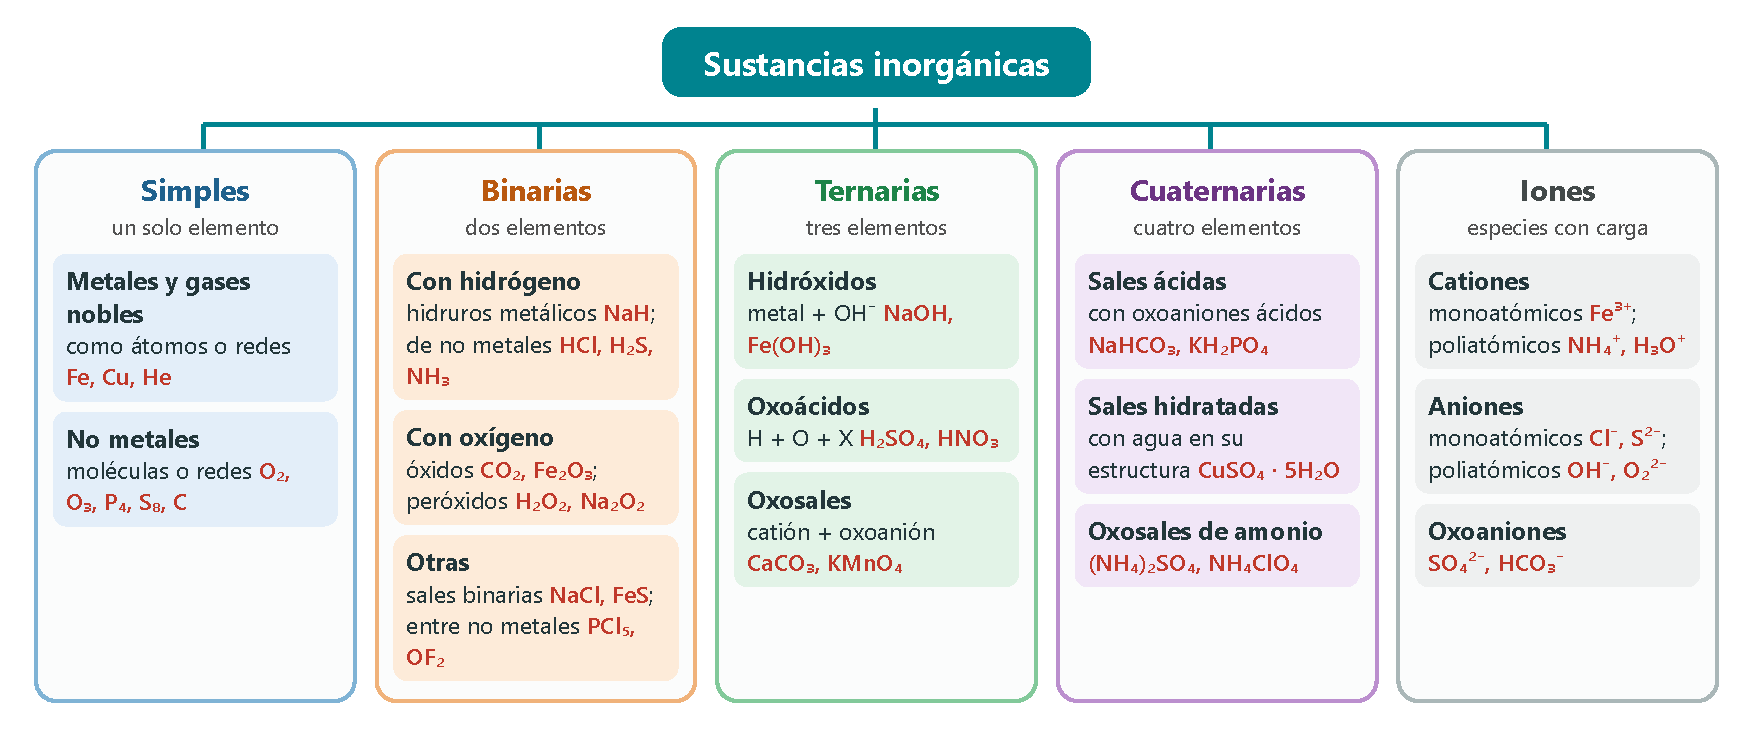
\includegraphics[width=\textwidth]{images/UD5/tipos_compuestos}
    \caption{Clasificación de las sustancias inorgánicas que estudiaremos en esta unidad, con algunos ejemplos.}
    \label{fig:ud5-tipos}
\end{figure}

\subsection{Número de carga y estado de oxidación}

\begin{definition}[Número de carga]
    Es la \textbf{carga eléctrica de un ion}. Se escribe con un número arábigo seguido del signo (\(+\) o \(-\)), entre
    paréntesis y justo detrás del nombre del ion, sin dejar espacio: el ion \ch{K+} es el ion potasio(1+) y el \ch{CO3^2-}, el ion
    trioxidocarbonato(2\nobreakdash--).
\end{definition}

El número de carga solo se puede usar para nombrar \textbf{compuestos iónicos}, que están formados por iones.

\begin{definition}[Estado de oxidación]
    Es la carga que tendría un átomo si todos sus enlaces fueran iónicos, es decir, si los electrones de cada enlace se los
    quedara por completo el átomo más electronegativo. Es positivo si el átomo «pierde» electrones y negativo si los «gana».
\end{definition}

El estado de oxidación se usa en las fórmulas y en los nombres como \textbf{número de oxidación}: un número romano, entre
paréntesis y sin espacio, detrás del nombre del elemento. Así, \ch{FeCO3} es el carbonato de hierro(II). En la
figura~\ref{fig:ud5-estados} tienes los estados de oxidación más frecuentes; algunos conviene saberlos de memoria:
\begin{itemize}
    \item Grupo 1 (alcalinos) y plata: \(+1\). Grupo 2 (alcalinotérreos), cinc y cadmio: \(+2\). Aluminio: \(+3\).
    \item Flúor: \(-1\). Oxígeno: \(-2\), salvo en los peróxidos (\(-1\)) y cuando se combina con el flúor.
    \item Hidrógeno: \(+1\) cuando se une a no metales y \(-1\) cuando se une a metales.
    \item Los elementos sin combinar (\ch{Fe}, \ch{O2}, \ch{P4}…) tienen estado de oxidación \textbf{cero}.
\end{itemize}

\begin{figure}[H]
    \centering
    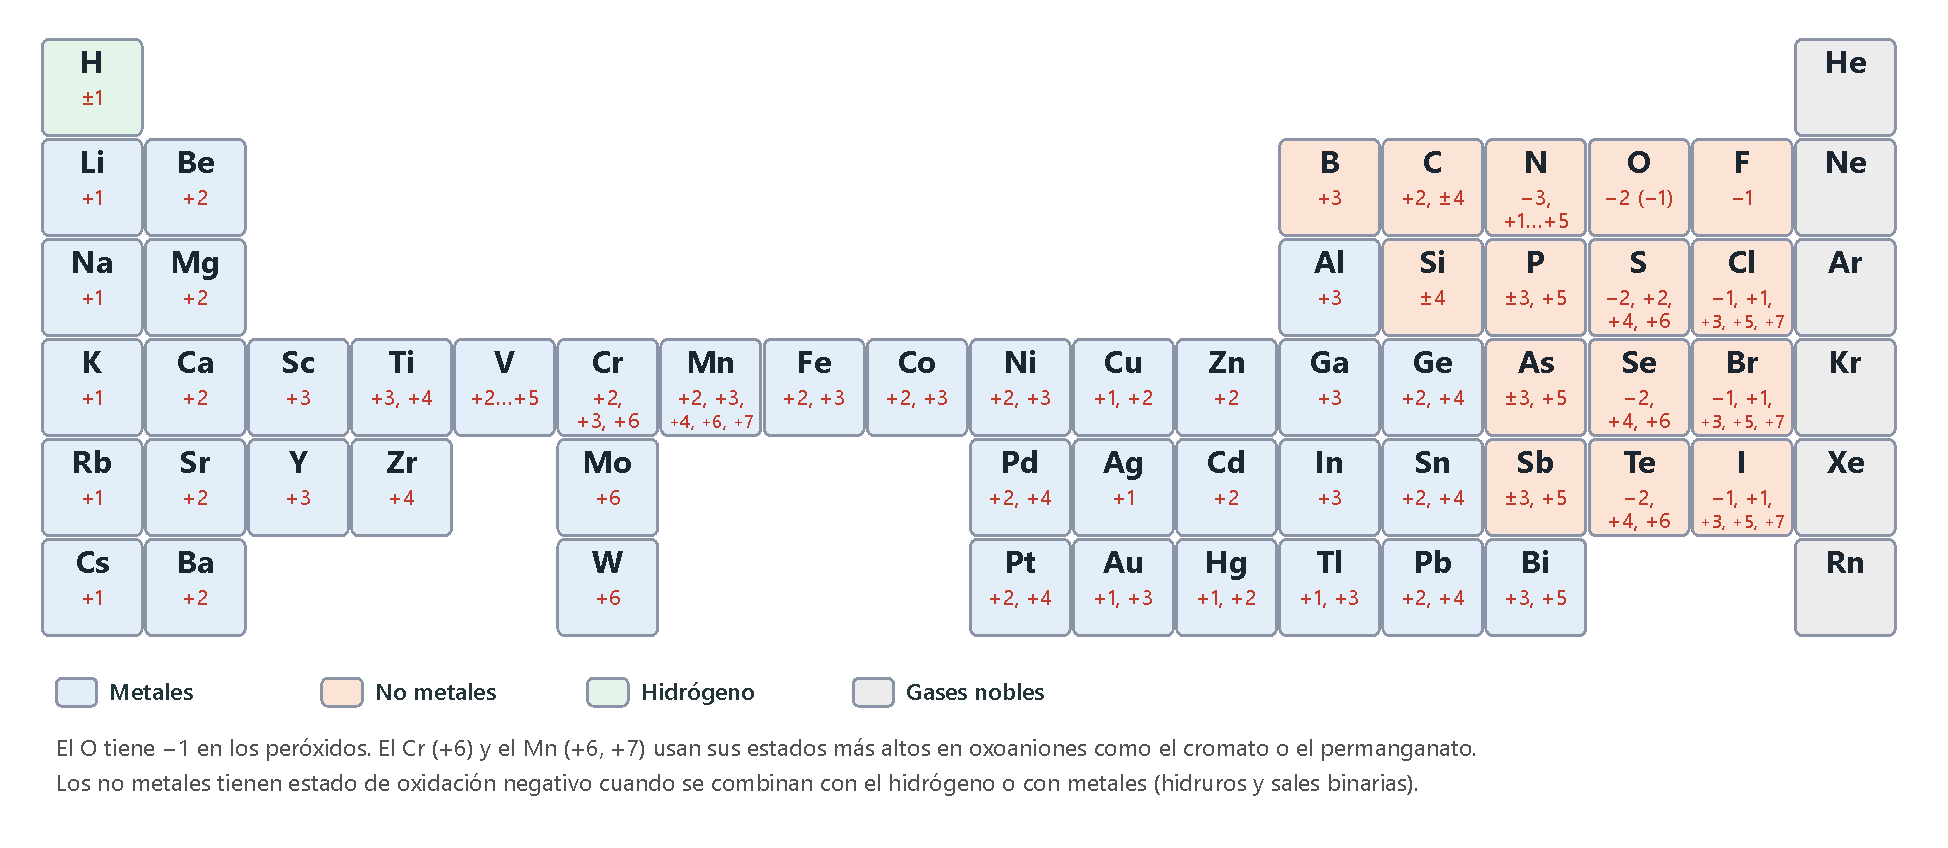
\includegraphics[width=\textwidth]{images/UD5/estados_oxidacion}
    \caption{Estados de oxidación más frecuentes de los elementos que usaremos en la unidad.}
    \label{fig:ud5-estados}
\end{figure}

\subsection{La regla de la suma}

\begin{definition}[Regla de la suma]
    En un compuesto \textbf{neutro}, la suma de los estados de oxidación de todos sus átomos (o de los números de carga de todos
    sus iones) es \textbf{cero}. En un \textbf{ion}, esa suma es igual a la \textbf{carga del ion}.
\end{definition}

Con esta regla y unos pocos valores memorizados puedes calcular el estado de oxidación de cualquier elemento en cualquier
compuesto.

\begin{example}
    \textbf{Calcular estados de oxidación.} Calcula el estado de oxidación del cromo en el \ch{K2Cr2O7}, del manganeso en el
    \ch{KMnO4}, del azufre en el \ch{Na2S2O3} y del nitrógeno en el ion \ch{NH4+}.

    \textbf{Solución.} Llamamos \(x\) al estado de oxidación desconocido y aplicamos la regla de la suma (K y Na, \(+1\);
    O, \(-2\); H, \(+1\)):
    \begin{itemize}
        \item \ch{K2Cr2O7}: \(2 \cdot (+1) + 2x + 7 \cdot (-2) = 0 \;\Rightarrow\; 2x = 12 \;\Rightarrow\; x = +6\).
        \item \ch{KMnO4}: \(+1 + x + 4 \cdot (-2) = 0 \;\Rightarrow\; x = +7\).
        \item \ch{Na2S2O3}: \(2 \cdot (+1) + 2x + 3 \cdot (-2) = 0 \;\Rightarrow\; 2x = 4 \;\Rightarrow\; x = +2\).
        \item \ch{NH4+}: \(x + 4 \cdot (+1) = +1 \;\Rightarrow\; x = -3\) (la suma es la carga del ion, no cero).
    \end{itemize}
\end{example}

\begin{exercise}
    Calcula el estado de oxidación del elemento destacado en negrita: a) \textbf{S} en \ch{H2SO3}; b) \textbf{P} en \ch{Ca3(PO4)2};
    c) \textbf{Cl} en \ch{ClO4-}; d) \textbf{C} en \ch{CH4}; e) \textbf{Fe} en \ch{Fe2O3}; f) \textbf{N} en \ch{NO2-}; g)
    \textbf{O} en \ch{BaO2}; h) \textbf{Cr} en \ch{CrO4^2-}.
    \begin{solu}
        a) \(2 + x - 6 = 0\): \textcolor{red}{\(+4\)}. b) El fosfato es \ch{PO4^3-}: \(x - 8 = -3\): \textcolor{red}{\(+5\)}.
        c) \(x - 8 = -1\): \textcolor{red}{\(+7\)}. d) \(x + 4 = 0\): \textcolor{red}{\(-4\)}. e) \(2x - 6 = 0\):
        \textcolor{red}{\(+3\)}. f) \(x - 4 = -1\): \textcolor{red}{\(+3\)}. g) \(2 + 2x = 0\): \textcolor{red}{\(-1\)} (es un
        peróxido). h) \(x - 8 = -2\): \textcolor{red}{\(+6\)}.
    \end{solu}
\end{exercise}

\begin{exercise}
    Usando la regla de la suma, indica si son posibles estas fórmulas y, si no lo son, corrígelas: a) \ch{CaCl}; b) \ch{Al2O3};
    c) \ch{KS}; d) \ch{Ba3N2}; e) \ch{LiO}; f) \ch{MgF2}.
    \begin{solu}
        a) \(+2 - 1 \neq 0\): \textcolor{red}{no; \ch{CaCl2}}. b) \(2 \cdot 3 + 3 \cdot (-2) = 0\): \textcolor{red}{sí}.
        c) \(+1 - 2 \neq 0\): \textcolor{red}{no; \ch{K2S}}. d) \(3 \cdot 2 + 2 \cdot (-3) = 0\): \textcolor{red}{sí}.
        e) \(+1 - 2 \neq 0\): \textcolor{red}{no; \ch{Li2O}}. f) \(+2 + 2 \cdot (-1) = 0\): \textcolor{red}{sí}.
    \end{solu}
\end{exercise}

\subsection{La secuencia de los elementos}

Al escribir una fórmula hay que colocar los símbolos en un \textbf{orden determinado}. La IUPAC ha fijado por convenio una
\textbf{secuencia de los elementos} (figura~\ref{fig:ud5-secuencia}): se recorre la tabla periódica empezando por los gases nobles
y avanzando grupo a grupo, de abajo arriba dentro de cada grupo, con el hidrógeno colocado entre los grupos 15 y 16, hasta terminar
en el flúor.

\begin{definition}[Orden en la fórmula]
    De dos elementos, se escribe a la \textbf{izquierda} el que aparece \textbf{antes} en la secuencia, que hace el papel de
    \textbf{electropositivo}, y a la \textbf{derecha} el que aparece \textbf{después}, que hace el papel de
    \textbf{electronegativo}.
\end{definition}

\begin{figure}[H]
    \centering
    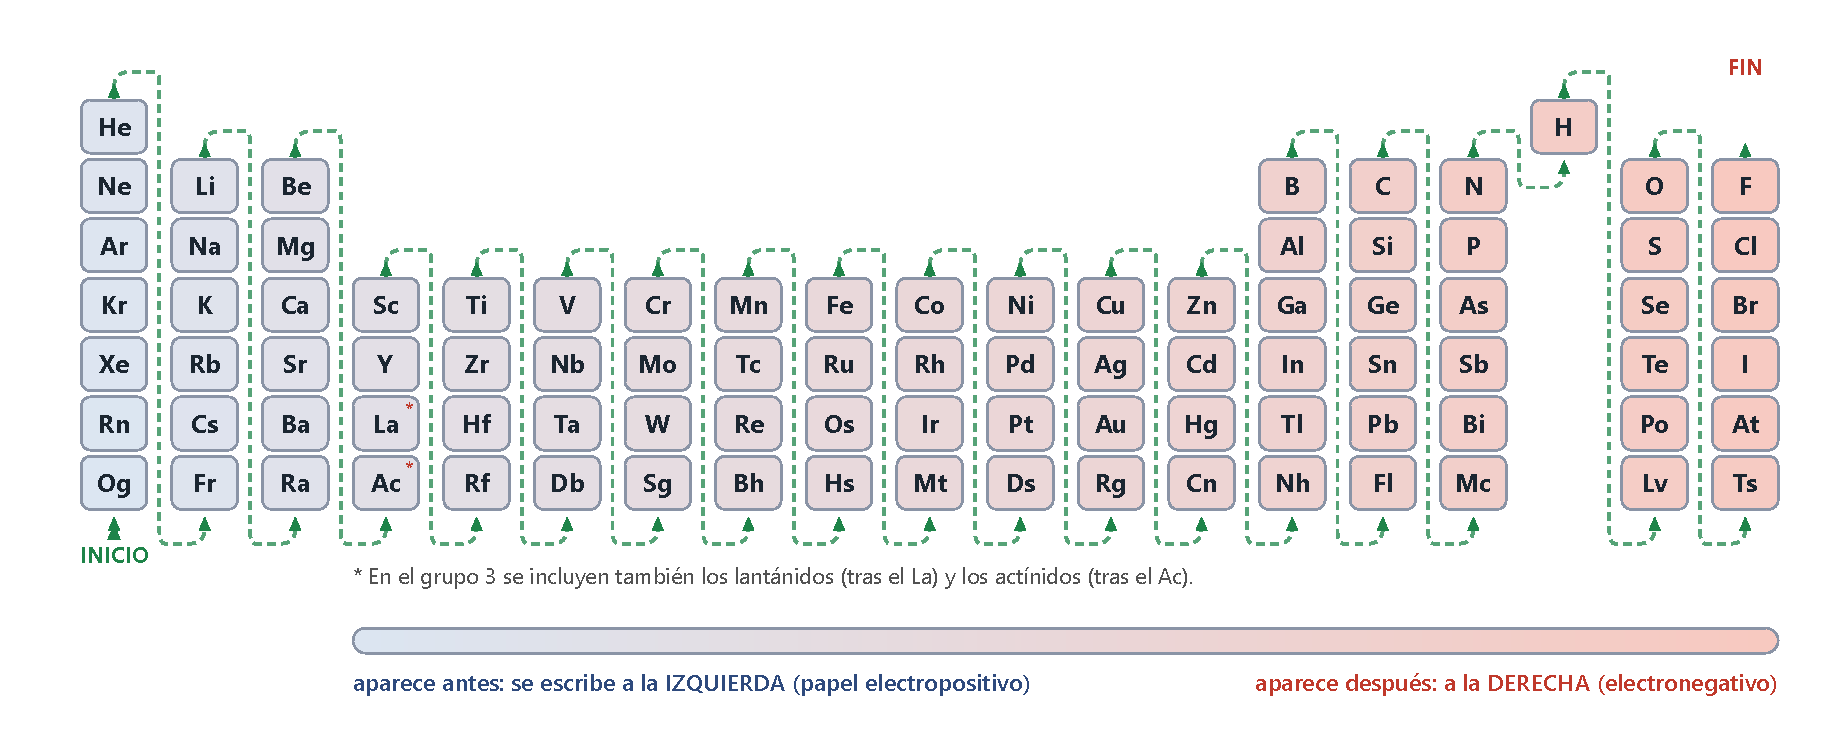
\includegraphics[width=\textwidth]{images/UD5/secuencia_elementos}
    \caption{Secuencia de los elementos para formular y nombrar (IUPAC 2005). Se avanza de abajo arriba en cada grupo y de un
    grupo al siguiente siguiendo las flechas.}
    \label{fig:ud5-secuencia}
\end{figure}

Esta secuencia se parece mucho a ordenar los elementos por su electronegatividad, que era el criterio antiguo, pero no es igual.
Por ejemplo, el oxígeno aparece antes que los halógenos: la fórmula es \ch{OCl2} y no \ch{Cl2O}. En el amoniaco, el nitrógeno va
antes que el hidrógeno (\ch{NH3}), y en el agua el hidrógeno va antes que el oxígeno (\ch{H2O}).

\subsection{Sistemas de nomenclatura}

La IUPAC recomienda tres sistemas de nomenclatura; además, acepta algunos nombres tradicionales.

\begin{table}[H]
    \centering
    \caption{Sistemas de nomenclatura}
    \vspace{-5pt}
    \begin{tabular}{@{}L{3.2cm}L{11cm}@{}}
        \toprule
        \textbf{Sistema} & \textbf{En qué consiste} \\
        \midrule
        De composición o estequiométrica & Se basa en la \textbf{composición}: indica los elementos y su proporción, pero no la
        estructura. La proporción se da con \textbf{prefijos multiplicadores} (dióxido de carbono), con el \textbf{número de
        oxidación} (óxido de carbono(IV)) o, solo en compuestos iónicos, con el \textbf{número de carga} (óxido de hierro(3+)). La
        única contracción admitida es monóxido: se escribe tetraóxido, pentaóxido (no «tetróxido», «pentóxido»). \\[3pt]
        De adición & Considera que el compuesto tiene un \textbf{átomo central} unido a otros átomos o grupos, los
        \textbf{ligandos}. No se usa para compuestos binarios. Es la base de los nombres de los oxoácidos. \\[3pt]
        De sustitución & Parte de un compuesto progenitor con nombre propio (el \textbf{hidruro progenitor}) y sustituye
        algunos de sus átomos de hidrógeno. Es la base de la química orgánica. \\[3pt]
        Nombres tradicionales & La IUPAC acepta unos pocos nombres muy extendidos que no siguen reglas sistemáticas: agua,
        amoniaco, ácido sulfúrico… \\[3pt]
        Nomenclatura de hidrógeno & Variante de la de adición para compuestos con hidrógeno cuya estructura no se conoce o no se
        quiere indicar: dihidrogeno(tetraoxidosulfato). \\
        \bottomrule
    \end{tabular}
    \label{tab:ud5-sistemas}
\end{table}

%========================================================================================
\section{Sustancias simples}\label{sec:ud5-simples}
%========================================================================================

\begin{definition}[Sustancia simple]
    Es la formada por átomos de un \textbf{mismo elemento}. Su estado de oxidación es siempre \textbf{cero}.
\end{definition}

\begin{itemize}
    \item Si la sustancia está formada por \textbf{átomos sueltos} (los gases nobles) o por \textbf{redes cristalinas} (los
    metales y algunos no metales, como el carbono o el silicio), se formula con el símbolo y se nombra con el nombre del
    elemento: \ch{He}, helio; \ch{Au}, oro; \ch{C}, carbono.
    \item Si está formada por \textbf{moléculas}, la fórmula lleva un \textbf{subíndice} con el número de átomos y el nombre
    lleva el \textbf{prefijo multiplicador} correspondiente: \ch{H2}, dihidrógeno; \ch{O3}, trioxígeno; \ch{P4}, tetrafósforo;
    \ch{S8}, octaazufre.
\end{itemize}

El prefijo \textit{mono} solo se usa si el elemento no se presenta de forma monoatómica en la naturaleza: \ch{N} es
mononitrógeno, una especie muy reactiva distinta del \ch{N2} del aire (dinitrógeno). La IUPAC acepta los nombres \textbf{oxígeno}
para el \ch{O2} y \textbf{ozono} para el \ch{O3}.

\begin{exercise}
    Nombra o formula: a) \ch{Ne}; b) \ch{Br2}; c) \ch{Ag}; d) \ch{S8}; e) \ch{F2}; f) \ch{O}; g) argón; h) cobre; i) ozono;
    j) dinitrógeno; k) tetrafósforo; l) diyodo.
    \begin{solu}
        a) \textcolor{red}{neón}; b) \textcolor{red}{dibromo}; c) \textcolor{red}{plata}; d) \textcolor{red}{octaazufre};
        e) \textcolor{red}{diflúor}; f) \textcolor{red}{monooxígeno}; g) \textcolor{red}{\ch{Ar}}; h) \textcolor{red}{\ch{Cu}};
        i) \textcolor{red}{\ch{O3}}; j) \textcolor{red}{\ch{N2}}; k) \textcolor{red}{\ch{P4}}; l) \textcolor{red}{\ch{I2}}.
    \end{solu}
\end{exercise}

%========================================================================================
\section{Iones}\label{sec:ud5-iones}
%========================================================================================

\begin{definition}[Ion]
    Es una especie química con carga eléctrica, porque ha \textbf{ganado} o \textbf{perdido} electrones. Si su carga es
    \textbf{negativa} se llama \textbf{anión}, y si es \textbf{positiva}, \textbf{catión}.
\end{definition}

\subsection{Iones monoatómicos}

Proceden de un solo átomo. Los estados de oxidación de la figura~\ref{fig:ud5-estados} te dicen qué iones son los más probables:
el potasio (\(+1\)) forma \ch{K+}; el hierro (\(+2\), \(+3\)), \ch{Fe^2+} y \ch{Fe^3+}, y el azufre, como no metal, tiende a
ganar electrones y formar \ch{S^2-}.

\paragraph{Formular.} Se escribe el símbolo y, como superíndice, la carga: primero el número y después el signo. El 1 no se
escribe: \ch{Cl-}, \ch{N^3-}, \ch{K+}, \ch{Fe^3+}.

\paragraph{Aniones monoatómicos.} Se nombran con la raíz del nombre del elemento terminada en \textbf{-uro} y, si hace falta, el
número de carga: \ch{N^3-} es nitruro(3\nobreakdash--), o simplemente \textbf{nitruro}, porque el nitrógeno solo forma un anión. Algunos
elementos usan la raíz latina: \ch{S^2-}, \textbf{sulfuro}. La excepción más importante es el \ch{O^2-}, que se llama
\textbf{óxido}.

\paragraph{Cationes monoatómicos.} Se nombran con el nombre del elemento seguido \textbf{siempre} del número de carga, aunque
sea único: \ch{K+} es el potasio(1+) y \ch{Fe^3+}, el hierro(3+).

\subsection{Iones poliatómicos}

\paragraph{Homopoliatómicos.} Están formados por varios átomos de un \textbf{mismo elemento}. Se nombran con prefijos
multiplicadores, y el número de átomos se escribe como subíndice. Algunos tienen nombres no sistemáticos aceptados por la IUPAC.

\begin{table}[H]
    \centering
    \caption{Iones poliatómicos frecuentes}
    \vspace{-5pt}
    \begin{tabular}{@{}lL{4.6cm}@{\hspace{1cm}}lL{4.6cm}@{}}
        \toprule
        \textbf{Fórmula} & \textbf{Nombre} & \textbf{Fórmula} & \textbf{Nombre} \\
        \midrule
        \ch{Hg2^2+} & dimercurio(2+) & \ch{O2^2-} & dióxido(2\nobreakdash--) o \textbf{peróxido} \\[3pt]
        \ch{I3-} & triyoduro(1\nobreakdash--) & \ch{C2^2-} & dicarburo(2\nobreakdash--) o \textbf{acetiluro} \\[3pt]
        \ch{NH4+} & azanio o \textbf{amonio} & \ch{OH-} & hidróxido \\[3pt]
        \ch{H3O+} & oxidanio u \textbf{oxonio} & \ch{CN-} & cianuro \\
        \bottomrule
    \end{tabular}
    \label{tab:ud5-poliatomicos}
\end{table}

\paragraph{Heteropoliatómicos.} Tienen \textbf{más de un elemento}. Los más importantes son los \textbf{oxoaniones}, como el
\ch{CO3^2-}, que estudiaremos en la sección~\ref{sec:ud5-oxoaniones}. Los cuatro de la tabla~\ref{tab:ud5-poliatomicos} (amonio,
oxonio, hidróxido y cianuro) conviene aprenderlos ya. Fíjate en que en el \ch{OH-} los símbolos no siguen la secuencia de los
elementos: es una excepción aceptada.

\begin{exercise}
    Nombra o formula estos iones: a) \ch{Br-}; b) \ch{Ca^2+}; c) \ch{Se^2-}; d) \ch{Cu+}; e) \ch{P^3-}; f) \ch{H3O+};
    g) \ch{Co^3+}; h) \ch{O2^2-}; i) yoduro; j) óxido; k) estaño(4+); l) amonio; m) hidróxido; n) plata(1+); ñ) fluoruro; o)
    mercurio(2+).
    \begin{solu}
        a) \textcolor{red}{bromuro}; b) \textcolor{red}{calcio(2+)}; c) \textcolor{red}{seleniuro}; d) \textcolor{red}{cobre(1+)};
        e) \textcolor{red}{fosfuro}; f) \textcolor{red}{oxonio (oxidanio)}; g) \textcolor{red}{cobalto(3+)}; h)
        \textcolor{red}{peróxido (dióxido(2\nobreakdash--))}; i) \textcolor{red}{\ch{I-}}; j) \textcolor{red}{\ch{O^2-}}; k)
        \textcolor{red}{\ch{Sn^4+}}; l) \textcolor{red}{\ch{NH4+}}; m) \textcolor{red}{\ch{OH-}}; n) \textcolor{red}{\ch{Ag+}};
        ñ) \textcolor{red}{\ch{F-}}; o) \textcolor{red}{\ch{Hg^2+}}.
    \end{solu}
\end{exercise}

%========================================================================================
\section{Compuestos binarios}\label{sec:ud5-binarios}
%========================================================================================

\begin{definition}[Compuesto binario]
    Es el formado por átomos de \textbf{dos elementos} diferentes. Se nombran con la nomenclatura de \textbf{composición} (y
    los hidruros de los grupos 13 a 17, también con la de \textbf{sustitución}).
\end{definition}

\paragraph{Formular.} El elemento que aparece \textbf{antes} en la secuencia (figura~\ref{fig:ud5-secuencia}) se escribe a la
\textbf{izquierda} y hace de \textbf{electropositivo}; el otro, a la derecha, hace de \textbf{electronegativo} y tiene estado de
oxidación negativo. Los \textbf{subíndices} se deducen de la \textbf{neutralidad}: la suma de los estados de oxidación (o de los
números de carga) tiene que ser cero.

\paragraph{Nombrar.} Se lee la fórmula de \textbf{derecha a izquierda}: primero el elemento electronegativo, con la terminación
\textbf{-uro} (u \textbf{óxido} si es el oxígeno), después «de» y el nombre del elemento electropositivo. La proporción se
indica de una de estas formas:
\begin{itemize}
    \item Con \textbf{prefijos multiplicadores} en los dos elementos: \ch{CaF2} es difluoruro de calcio. El prefijo
    \textit{mono} se puede omitir, salvo en monóxido.
    \item Con el \textbf{número de oxidación} del electropositivo: fluoruro de calcio(II).
    \item Con el \textbf{número de carga} del catión, solo si el compuesto es iónico: fluoruro de calcio(2+).
\end{itemize}
El número de oxidación o de carga solo se indica en el elemento electropositivo, y se puede \textbf{omitir} si ese elemento
solo tiene un estado de oxidación: \ch{CaF2} es, sencillamente, \textbf{fluoruro de calcio}.

\begin{example}
    \textbf{Formular un binario.} Formula el compuesto de calcio y flúor y nómbralo de todas las formas posibles.

    \textbf{Solución.} \textbf{1. Orden}: el calcio aparece antes que el flúor en la secuencia: \ch{Ca} a la izquierda y
    \ch{F} a la derecha. \textbf{2. Estados de oxidación}: \(\ch{Ca} = +2\) (su único valor) y \(\ch{F} = -1\).
    \textbf{3. Neutralidad}: \(1 \cdot (+2) + 2 \cdot (-1) = 0\): hacen falta dos átomos de F por cada átomo de Ca, y la fórmula
    es \ch{CaF2}. \textbf{4. Nombres}: difluoruro de calcio; fluoruro de calcio(II); fluoruro de calcio(2+), o simplemente
    \textbf{fluoruro de calcio}, porque el calcio solo tiene un estado de oxidación.
\end{example}

\subsection{Compuestos binarios con hidrógeno}\label{sec:ud5-hidruros}

La posición del hidrógeno en la fórmula depende del elemento con el que se combina.

\paragraph{Hidruros de los grupos 1 a 15.} El hidrógeno aparece después en la secuencia: se escribe a la \textbf{derecha}, hace
de electronegativo y tiene estado de oxidación \(-1\). Se nombran con la palabra \textbf{hidruro}, y la proporción se indica con
prefijos multiplicadores o con el número de oxidación del otro elemento, si tiene más de uno. Si el otro elemento es un metal, el
compuesto es iónico (contiene el ion hidruro, \ch{H-}) y también se puede usar el número de carga.

\paragraph{Hidruros de los grupos 16 y 17 (salvo el oxígeno).} El hidrógeno aparece antes en la secuencia: se escribe a la
\textbf{izquierda}, hace de electropositivo y tiene estado de oxidación \(+1\). Se nombran con el otro elemento terminado en
\textbf{-uro} seguido de «de hidrógeno». No son iónicos, así que no se usa el número de carga, y como el hidrógeno solo tiene un
estado de oxidación positivo, tampoco hace falta el número de oxidación. Sus \textbf{disoluciones acuosas} son ácidas y antes se
llamaban \textbf{ácidos hidrácidos} (ácido clorhídrico, ácido sulfhídrico): la IUPAC no acepta esos nombres para los compuestos
puros, porque son nombres de las disoluciones.

\begin{table}[H]
    \centering
    \caption{Nomenclatura de composición de algunos compuestos binarios con hidrógeno}
    \vspace{-5pt}
    \begin{tabular}{@{}lL{3.6cm}L{3.6cm}L{3.6cm}@{}}
        \toprule
        \textbf{Fórmula} & \textbf{Prefijos multiplicadores} & \textbf{Número de oxidación} & \textbf{Número de carga} \\
        \midrule
        \ch{CuH2} & dihidruro de cobre & hidruro de cobre(II) & hidruro de cobre(2+) \\[3pt]
        \ch{AlH3} & trihidruro de aluminio & hidruro de aluminio & hidruro de aluminio \\[3pt]
        \ch{NH3} & trihidruro de nitrógeno & hidruro de nitrógeno(III) & --- \\[3pt]
        \ch{CH4} & tetrahidruro de carbono & hidruro de carbono(IV) & --- \\[3pt]
        \ch{H2S} & sulfuro de dihidrógeno & sulfuro de hidrógeno & --- \\[3pt]
        \ch{HCl} & cloruro de hidrógeno & cloruro de hidrógeno & --- \\
        \bottomrule
    \end{tabular}
    \label{tab:ud5-hidruros}
\end{table}

\paragraph{Nomenclatura de sustitución.} Los hidruros de los grupos 13 a 17 son los \textbf{hidruros progenitores}, de los que
derivan muchos otros compuestos. Se nombran con la raíz del elemento y la terminación \textbf{-ano}. El agua y el amoniaco
mantienen sus nombres tradicionales, que son los recomendados.

\begin{table}[H]
    \centering
    \caption{Hidruros progenitores (nomenclatura de sustitución)}
    \vspace{-5pt}
    \begin{tabular}{@{}ll@{\hspace{0.8cm}}ll@{\hspace{0.8cm}}ll@{\hspace{0.8cm}}ll@{}}
        \toprule
        \multicolumn{2}{@{}c}{\textbf{Grupo 13 y 14}} & \multicolumn{2}{c}{\textbf{Grupo 15}} & \multicolumn{2}{c}{\textbf{Grupo
        16}} & \multicolumn{2}{c@{}}{\textbf{Grupo 17}} \\
        \midrule
        \ch{BH3} & borano & \ch{NH3} & azano, \textbf{amoniaco} & \ch{H2O} & oxidano, \textbf{agua} & \ch{HF} & fluorano \\[3pt]
        \ch{AlH3} & alumano & \ch{PH3} & fosfano & \ch{H2S} & sulfano & \ch{HCl} & clorano \\[3pt]
        \ch{CH4} & metano & \ch{AsH3} & arsano & \ch{H2Se} & selano & \ch{HBr} & bromano \\[3pt]
        \ch{SiH4} & silano & \ch{SbH3} & estibano & \ch{H2Te} & telano & \ch{HI} & yodano \\
        \bottomrule
    \end{tabular}
    \label{tab:ud5-progenitores}
\end{table}

De los progenitores derivan otras especies: el ion \ch{H3O+}, oxidanio, procede del oxidano (\ch{H2O}), y el \ch{NH4+}, azanio,
del azano (\ch{NH3}).

\begin{example}
    \textbf{Hidruros.} Nombra de todas las formas posibles: \ch{PbH4}, \ch{KH}, \ch{BH3}, \ch{H2Te} y \ch{GeH4}.

    \textbf{Solución.}
    \begin{itemize}
        \item \ch{PbH4}: tetrahidruro de plomo; hidruro de plomo(IV); hidruro de plomo(4+) (el plomo tiene \(+2\) y \(+4\): hay
        que indicarlo).
        \item \ch{KH}: hidruro de potasio (el potasio solo tiene \(+1\); con prefijos, monohidruro de potasio o hidruro de
        potasio).
        \item \ch{BH3}: trihidruro de boro; hidruro de boro; \textbf{borano}. No es iónico: no hay número de carga.
        \item \ch{H2Te}: telururo de dihidrógeno; telururo de hidrógeno; \textbf{telano}.
        \item \ch{GeH4}: tetrahidruro de germanio; hidruro de germanio(IV); \textbf{germano}.
    \end{itemize}
\end{example}

\begin{exercise}
    Nombra de todas las maneras posibles: a) \ch{NaH}; b) \ch{BaH2}; c) \ch{FeH3}; d) \ch{CoH2}; e) \ch{HBr}; f) \ch{H2Se};
    g) \ch{SnH4}; h) \ch{PH3}; i) \ch{AsH3}; j) \ch{HF}; k) \ch{AuH}; l) \ch{SiH4}.
    \begin{solu}
        a) \textcolor{red}{hidruro de sodio}. b) \textcolor{red}{dihidruro de bario; hidruro de bario}. c)
        \textcolor{red}{trihidruro de hierro; hidruro de hierro(III); hidruro de hierro(3+)}. d) \textcolor{red}{dihidruro de
        cobalto; hidruro de cobalto(II); hidruro de cobalto(2+)}. e) \textcolor{red}{bromuro de hidrógeno; bromano}. f)
        \textcolor{red}{seleniuro de dihidrógeno; seleniuro de hidrógeno; selano}. g) \textcolor{red}{tetrahidruro de estaño;
        hidruro de estaño(IV); hidruro de estaño(4+); estannano}. h) \textcolor{red}{trihidruro de fósforo; hidruro de
        fósforo(III); fosfano}. i) \textcolor{red}{trihidruro de arsénico; hidruro de arsénico(III); arsano}. j)
        \textcolor{red}{fluoruro de hidrógeno; fluorano}. k) \textcolor{red}{hidruro de oro; hidruro de oro(I); hidruro de
        oro(1+)}. l) \textcolor{red}{tetrahidruro de silicio; hidruro de silicio; silano}.
    \end{solu}
\end{exercise}

\begin{exercise}
    Formula: a) hidruro de litio; b) dihidruro de magnesio; c) hidruro de níquel(III); d) hidruro de cobre(1+); e) cloruro de
    hidrógeno; f) sulfuro de dihidrógeno; g) estibano; h) metano; i) hidruro de paladio(IV); j) yoduro de hidrógeno; k)
    trihidruro de cromo; l) azano.
    \begin{solu}
        a) \textcolor{red}{\ch{LiH}}; b) \textcolor{red}{\ch{MgH2}}; c) \textcolor{red}{\ch{NiH3}}; d) \textcolor{red}{\ch{CuH}};
        e) \textcolor{red}{\ch{HCl}}; f) \textcolor{red}{\ch{H2S}}; g) \textcolor{red}{\ch{SbH3}}; h) \textcolor{red}{\ch{CH4}};
        i) \textcolor{red}{\ch{PdH4}}; j) \textcolor{red}{\ch{HI}}; k) \textcolor{red}{\ch{CrH3}}; l) \textcolor{red}{\ch{NH3}}.
    \end{solu}
\end{exercise}

\subsection{Compuestos binarios con oxígeno}\label{sec:ud5-oxidos}

\paragraph{Óxidos.} Son las combinaciones binarias del oxígeno con cualquier elemento \textbf{excepto los halógenos}. Pueden ser
\textbf{metálicos} (\ch{Fe2O3}) o \textbf{no metálicos} (\ch{CO2}). El oxígeno se escribe a la \textbf{derecha} y tiene estado
de oxidación \(-2\).

\begin{itemize}
    \item \textbf{Nombrar}: con prefijos multiplicadores (dióxido de carbono; el \textit{mono} se puede omitir si no hay
    ambigüedad, pero no en el \ch{CO}, monóxido de carbono, para distinguirlo del \ch{CO2}); con el número de oxidación del
    otro elemento, calculado con la regla de la suma (en el \ch{CO2}, \(x + 2 \cdot (-2) = 0\), \(x = +4\): óxido de
    carbono(IV)), o, solo en los óxidos metálicos, que son iónicos, con el número de carga (\ch{Fe2O3}, óxido de hierro(3+)).
    \item \textbf{Formular}: si el nombre tiene prefijos, basta con escribirlos como subíndices (pentaóxido de difósforo,
    \ch{P2O5}); si tiene número de oxidación o de carga, se calculan los subíndices con la regla de la suma y se simplifican si se
    puede (óxido de azufre(VI): \(+6\) y \(-2\), \ch{S2O6} \(\rightarrow\) \ch{SO3}).
\end{itemize}

\paragraph{Haluros de oxígeno.} Los halógenos aparecen \textbf{después} que el oxígeno en la secuencia: en sus combinaciones con
el oxígeno, el halógeno va a la derecha y hace de electronegativo. \textbf{No son óxidos}, sino haluros, y se nombran
\textbf{solo con prefijos multiplicadores}: \ch{OCl2} es el dicloruro de oxígeno y \ch{O5Br2}, el dibromuro de pentaoxígeno.

\begin{table}[H]
    \centering
    \caption{Nomenclatura de algunos compuestos binarios con oxígeno}
    \vspace{-5pt}
    \begin{tabular}{@{}lL{3.6cm}L{3.6cm}L{3.6cm}@{}}
        \toprule
        \textbf{Fórmula} & \textbf{Prefijos multiplicadores} & \textbf{Número de oxidación} & \textbf{Número de carga} \\
        \midrule
        \ch{CO} & monóxido de carbono & óxido de carbono(II) & --- \\[3pt]
        \ch{Cu2O} & monóxido de dicobre & óxido de cobre(I) & óxido de cobre(1+) \\[3pt]
        \ch{Au2O3} & trióxido de dioro & óxido de oro(III) & óxido de oro(3+) \\[3pt]
        \ch{SrO} & óxido de estroncio & óxido de estroncio & óxido de estroncio \\[3pt]
        \ch{SO3} & trióxido de azufre & óxido de azufre(VI) & --- \\[3pt]
        \ch{N2O5} & pentaóxido de dinitrógeno & óxido de nitrógeno(V) & --- \\[3pt]
        \ch{O3Cl2} & dicloruro de trioxígeno & --- & --- \\
        \bottomrule
    \end{tabular}
    \label{tab:ud5-oxidos}
\end{table}

\paragraph{Peróxidos.} Son combinaciones de un elemento con el anión \ch{O2^2-}, llamado \textbf{peróxido} o dióxido(2\nobreakdash--). En
ellos, cada oxígeno tiene estado de oxidación \(-1\).
\begin{itemize}
    \item Con \textbf{prefijos multiplicadores} se nombran como los óxidos: \ch{Na2O2} es el dióxido de disodio.
    \item Con el \textbf{número de oxidación}, se usa la palabra peróxido: \ch{BaO2} es el peróxido de bario.
    \item Con \textbf{números de carga} se nombran los dos iones: \ch{FeO2} es el dióxido(2\nobreakdash--) de hierro(2+).
\end{itemize}
Ten cuidado al calcular estados de oxidación: el ion \ch{O2^2-} tiene \textbf{carga \(-2\)} y \textbf{dos} átomos de oxígeno.
En el \ch{FeO2}, \(x + 2 \cdot (-1) = 0\) da \(x = +2\) para el hierro; también se puede razonar que un \ch{Fe} se une a un
\ch{O2^2-}, así que el catión es \ch{Fe^2+}. ¡No confundas el \ch{FeO2}, peróxido de hierro(II), con un óxido de hierro(IV)!
Por eso, en la fórmula de un peróxido \textbf{no se simplifica} el subíndice del oxígeno: el peróxido de hierro(III) tiene
\ch{Fe^3+} y \ch{O2^2-}; con 2 hierros y 3 peróxidos hay 6 cargas de cada signo, y la fórmula es \ch{Fe2(O2)3} \(=\)
\ch{Fe2O6}. La IUPAC acepta el nombre \textbf{agua oxigenada} para el \ch{H2O2}.

\begin{example}
    \textbf{Óxidos y peróxidos.} a) Nombra \ch{Mn2O7}, \ch{PbO2}, \ch{K2O2} y \ch{OF2}. b) Formula el óxido de cromo(III), el
    peróxido de cinc y el dióxido(2\nobreakdash--) de cobre(1+).

    \textbf{Solución.} a) \ch{Mn2O7}: heptaóxido de dimanganeso; óxido de manganeso(VII) (\(2x - 14 = 0\), \(x = +7\)); óxido
    de manganeso(7+). \ch{PbO2}: es un óxido, no un peróxido, porque el plomo puede tener \(+4\): dióxido de plomo; óxido de
    plomo(IV); óxido de plomo(4+). \ch{K2O2}: el potasio solo puede tener \(+1\), así que cada O tiene \(-1\): es un peróxido.
    Dióxido de dipotasio; peróxido de potasio; dióxido(2\nobreakdash--) de potasio. \ch{OF2}: el flúor va después del oxígeno; es un
    haluro: difluoruro de oxígeno.

    b) Óxido de cromo(III): \ch{Cr^3+} y \ch{O^2-}: \ch{Cr2O3}. Peróxido de cinc: \ch{Zn^2+} y \ch{O2^2-}, uno de cada:
    \ch{ZnO2}. Dióxido(2\nobreakdash--) de cobre(1+): dos \ch{Cu+} por cada \ch{O2^2-}: \ch{Cu2O2}.
\end{example}

\begin{exercise}
    Nombra de todas las maneras posibles: a) \ch{MgO}; b) \ch{Fe2O3}; c) \ch{SO2}; d) \ch{Ni2O3}; e) \ch{N2O3}; f) \ch{Na2O};
    g) \ch{Cl2O7}; h) \ch{HgO}; i) \ch{SnO2}; j) \ch{O5Cl2}; k) \ch{Cl2O}; l) \ch{SiO2}.
    \begin{solu}
        a) \textcolor{red}{óxido de magnesio}. b) \textcolor{red}{trióxido de dihierro; óxido de hierro(III); óxido de
        hierro(3+)}. c) \textcolor{red}{dióxido de azufre; óxido de azufre(IV)}. d) \textcolor{red}{trióxido de diníquel; óxido de
        níquel(III); óxido de níquel(3+)}. e) \textcolor{red}{trióxido de dinitrógeno; óxido de nitrógeno(III)}. f)
        \textcolor{red}{óxido de disodio; óxido de sodio}. g) \textcolor{red}{Fórmula mal escrita}: el O va antes que el Cl en
        la secuencia; es \ch{O7Cl2}, \textcolor{red}{dicloruro de heptaoxígeno}. h) \textcolor{red}{monóxido de mercurio; óxido
        de mercurio(II); óxido de mercurio(2+)}. i) \textcolor{red}{dióxido de estaño; óxido de estaño(IV); óxido de
        estaño(4+)}. j) \textcolor{red}{dicloruro de pentaoxígeno}. k) \textcolor{red}{Debe escribirse \ch{OCl2}: dicloruro de
        oxígeno}. l) \textcolor{red}{dióxido de silicio; óxido de silicio}.
    \end{solu}
\end{exercise}

\begin{exercise}
    Formula: a) óxido de litio; b) óxido de cobalto(II); c) pentaóxido de dinitrógeno; d) óxido de plomo(IV); e) monóxido de
    dicobre; f) óxido de vanadio(V); g) dicloruro de oxígeno; h) óxido de oro(3+); i) óxido de selenio(VI); j) dibromuro de
    trioxígeno; k) trióxido de diboro; l) óxido de manganeso(IV).
    \begin{solu}
        a) \textcolor{red}{\ch{Li2O}}; b) \textcolor{red}{\ch{CoO}}; c) \textcolor{red}{\ch{N2O5}}; d) \textcolor{red}{\ch{PbO2}};
        e) \textcolor{red}{\ch{Cu2O}}; f) \textcolor{red}{\ch{V2O5}}; g) \textcolor{red}{\ch{OCl2}}; h)
        \textcolor{red}{\ch{Au2O3}}; i) \textcolor{red}{\ch{SeO3}}; j) \textcolor{red}{\ch{O3Br2}}; k) \textcolor{red}{\ch{B2O3}};
        l) \textcolor{red}{\ch{MnO2}}.
    \end{solu}
\end{exercise}

\begin{exercise}
    a) Nombra de todas las maneras posibles: \ch{Li2O2}, \ch{SrO2}, \ch{CuO2}, \ch{H2O2}, \ch{Cs2O2}, \ch{Hg2O2}. b) Formula:
    peróxido de calcio, dióxido de dirrubidio, peróxido de níquel(II), dióxido(2\nobreakdash--) de plata(1+), peróxido de cobalto(III).
    \begin{solu}
        a) \ch{Li2O2}: \textcolor{red}{dióxido de dilitio; peróxido de litio; dióxido(2\nobreakdash--) de litio}. \ch{SrO2}:
        \textcolor{red}{dióxido de estroncio; peróxido de estroncio}. \ch{CuO2}: \textcolor{red}{dióxido de cobre; peróxido de
        cobre(II); dióxido(2\nobreakdash--) de cobre(2+)}. \ch{H2O2}: \textcolor{red}{agua oxigenada; dióxido de dihidrógeno; peróxido de
        hidrógeno}. \ch{Cs2O2}: \textcolor{red}{dióxido de dicesio; peróxido de cesio}. \ch{Hg2O2}: \textcolor{red}{dióxido de
        dimercurio; peróxido de mercurio(I)} (contiene \ch{Hg2^2+} y \ch{O2^2-}). b) \textcolor{red}{\ch{CaO2}, \ch{Rb2O2},
        \ch{NiO2}, \ch{Ag2O2}, \ch{Co2O6}}.
    \end{solu}
\end{exercise}

\subsection{Otros compuestos binarios}\label{sec:ud5-sales-binarias}

Todo lo anterior vale para el resto de compuestos binarios. Distinguimos dos tipos:

\paragraph{Sales binarias (metal y no metal).} Son compuestos \textbf{iónicos}. El metal se escribe a la izquierda y el no
metal, a la derecha, con su estado de oxidación negativo. Los subíndices se calculan con la regla de la suma. Se nombra primero
el no metal con la terminación \textbf{-uro} y después el metal, con prefijos, número de oxidación o número de carga: \ch{FeF2}
es el difluoruro de hierro, el fluoruro de hierro(II) o el fluoruro de hierro(2+).

\paragraph{Compuestos entre no metales.} La secuencia de los elementos decide cuál va a la derecha: ese hace de
electronegativo y tiene estado de oxidación negativo. Se nombra primero el de la derecha terminado en \textbf{-uro}. Como no son
iónicos, \textbf{no} se usa el número de carga: \ch{PCl5} es el pentacloruro de fósforo o el cloruro de fósforo(V).

\begin{example}
    \textbf{Sales binarias.} a) Nombra \ch{CuBr2}, \ch{Al2S3}, \ch{SF6} y \ch{BrF3}. b) Formula el sulfuro de hierro(III), el
    nitruro de magnesio y el tricloruro de fósforo.

    \textbf{Solución.} a) \ch{CuBr2}: dibromuro de cobre; bromuro de cobre(II); bromuro de cobre(2+). \ch{Al2S3}: trisulfuro de
    dialuminio; sulfuro de aluminio. \ch{SF6}: hexafluoruro de azufre; fluoruro de azufre(VI). \ch{BrF3}: el bromo aparece
    antes que el flúor en la secuencia: trifluoruro de bromo; fluoruro de bromo(III).

    b) Sulfuro de hierro(III): \ch{Fe^3+} y \ch{S^2-}; el mínimo común múltiplo de 3 y 2 es 6: dos \ch{Fe} y tres \ch{S},
    \ch{Fe2S3}. Nitruro de magnesio: \ch{Mg^2+} y \ch{N^3-}: \ch{Mg3N2}. Tricloruro de fósforo: \ch{PCl3}.
\end{example}

\begin{exercise}
    Nombra de todas las maneras posibles: a) \ch{KBr}; b) \ch{CaS}; c) \ch{FeCl2}; d) \ch{PbI4}; e) \ch{AgCl}; f) \ch{Cu2S};
    g) \ch{CoBr3}; h) \ch{SnCl4}; i) \ch{Li3N}; j) \ch{CS2}; k) \ch{NCl3}; l) \ch{IF5}; m) \ch{BN}; n) \ch{SiC}.
    \begin{solu}
        a) \textcolor{red}{bromuro de potasio}. b) \textcolor{red}{sulfuro de calcio}. c) \textcolor{red}{dicloruro de hierro;
        cloruro de hierro(II); cloruro de hierro(2+)}. d) \textcolor{red}{tetrayoduro de plomo; yoduro de plomo(IV); yoduro de
        plomo(4+)}. e) \textcolor{red}{cloruro de plata}. f) \textcolor{red}{sulfuro de dicobre; sulfuro de cobre(I); sulfuro de
        cobre(1+)}. g) \textcolor{red}{tribromuro de cobalto; bromuro de cobalto(III); bromuro de cobalto(3+)}. h)
        \textcolor{red}{tetracloruro de estaño; cloruro de estaño(IV); cloruro de estaño(4+)}. i) \textcolor{red}{nitruro de
        trilitio; nitruro de litio}. j) \textcolor{red}{disulfuro de carbono; sulfuro de carbono(IV)}. k)
        \textcolor{red}{tricloruro de nitrógeno; cloruro de nitrógeno(III)}. l) \textcolor{red}{pentafluoruro de yodo; fluoruro de
        yodo(V)}. m) \textcolor{red}{nitruro de boro}. n) \textcolor{red}{carburo de silicio}.
    \end{solu}
\end{exercise}

\begin{exercise}
    Formula: a) cloruro de sodio; b) sulfuro de aluminio; c) bromuro de mercurio(II); d) yoduro de cobre(1+); e) fluoruro de
    estaño(II); f) seleniuro de potasio; g) trifluoruro de boro; h) cloruro de azufre(II); i) tetracloruro de silicio; j)
    sulfuro de manganeso(IV); k) nitruro de calcio; l) heptafluoruro de yodo.
    \begin{solu}
        a) \textcolor{red}{\ch{NaCl}}; b) \textcolor{red}{\ch{Al2S3}}; c) \textcolor{red}{\ch{HgBr2}}; d) \textcolor{red}{\ch{CuI}};
        e) \textcolor{red}{\ch{SnF2}}; f) \textcolor{red}{\ch{K2Se}}; g) \textcolor{red}{\ch{BF3}}; h) \textcolor{red}{\ch{SCl2}};
        i) \textcolor{red}{\ch{SiCl4}}; j) \textcolor{red}{\ch{MnS2}}; k) \textcolor{red}{\ch{Ca3N2}}; l) \textcolor{red}{\ch{IF7}}.
    \end{solu}
\end{exercise}

%========================================================================================
\section{Compuestos ternarios y cuaternarios}\label{sec:ud5-ternarios}
%========================================================================================

Nos ocuparemos ahora de los \textbf{hidróxidos}, \textbf{oxoácidos}, \textbf{oxoaniones}, \textbf{oxosales}, \textbf{sales
ácidas} y \textbf{sales hidratadas}, compuestos formados por tres o cuatro elementos.

\subsection{Hidróxidos}

\begin{definition}[Hidróxido]
    Es un compuesto formado por un \textbf{catión metálico} y el ion \textbf{hidróxido}, \ch{OH-}.
\end{definition}

Aunque son ternarios, se formulan y se nombran como si fueran binarios, con la nomenclatura de composición. Como el número de
carga del \ch{OH-} es \(-1\), el número de grupos \ch{OH} coincide con la carga del catión: el \ch{Fe(OH)3} es el trihidróxido
de hierro, el hidróxido de hierro(III) o el hidróxido de hierro(3+). Al formular, si hay más de un grupo \ch{OH}, se escribe
entre paréntesis: el hidróxido de cobre(2+) es \ch{Cu(OH)2}.

\begin{example}
    \textbf{Hidróxidos.} a) Nombra \ch{KOH}, \ch{Sn(OH)2} y \ch{Cr(OH)3}. b) Formula el hidróxido de calcio y el hidróxido de
    plomo(IV).

    \textbf{Solución.} a) \ch{KOH}: hidróxido de potasio. \ch{Sn(OH)2}: dihidróxido de estaño; hidróxido de estaño(II);
    hidróxido de estaño(2+). \ch{Cr(OH)3}: trihidróxido de cromo; hidróxido de cromo(III); hidróxido de cromo(3+).
    b) \ch{Ca(OH)2} y \ch{Pb(OH)4}.
\end{example}

\begin{exercise}
    a) Nombra de todas las maneras posibles: \ch{LiOH}, \ch{Ba(OH)2}, \ch{Al(OH)3}, \ch{Ni(OH)2}, \ch{AgOH}, \ch{Au(OH)3},
    \ch{Zn(OH)2}, \ch{Pt(OH)4}. b) Formula: hidróxido de sodio, hidróxido de cobalto(III), dihidróxido de magnesio, hidróxido
    de cobre(1+), hidróxido de mercurio(II), tetrahidróxido de titanio.
    \begin{solu}
        a) \textcolor{red}{hidróxido de litio}; \textcolor{red}{dihidróxido de bario, hidróxido de bario};
        \textcolor{red}{trihidróxido de aluminio, hidróxido de aluminio}; \textcolor{red}{dihidróxido de níquel, hidróxido de
        níquel(II), hidróxido de níquel(2+)}; \textcolor{red}{hidróxido de plata}; \textcolor{red}{trihidróxido de oro,
        hidróxido de oro(III), hidróxido de oro(3+)}; \textcolor{red}{dihidróxido de cinc, hidróxido de cinc};
        \textcolor{red}{tetrahidróxido de platino, hidróxido de platino(IV), hidróxido de platino(4+)}.
        b) \textcolor{red}{\ch{NaOH}, \ch{Co(OH)3}, \ch{Mg(OH)2}, \ch{CuOH}, \ch{Hg(OH)2}, \ch{Ti(OH)4}}.
    \end{solu}
\end{exercise}

\subsection{Oxoácidos}\label{sec:ud5-oxoacidos}

\begin{definition}[Oxoácido]
    Es un compuesto ternario formado por \textbf{hidrógeno}, \textbf{oxígeno} y otro elemento, que suele ser un \textbf{no
    metal} (y a veces un metal de transición con estado de oxidación alto, como el Cr con \(+6\) o el Mn con \(+6\) y \(+7\)).
    Su fórmula general es \(\mathrm{H}_a\mathrm{X}_b\mathrm{O}_c\). En ellos, el oxígeno tiene estado de oxidación \(-2\) y el hidrógeno, \(+1\).
\end{definition}

\paragraph{Nombres tradicionales.} La nomenclatura tradicional está en desuso, pero la IUPAC \textbf{admite y recomienda} los
nombres tradicionales de una \textbf{lista cerrada} de oxoácidos muy comunes (tabla~\ref{tab:ud5-oxoacidos}); los que no
están en la lista no deben nombrarse así. En estos nombres, los prefijos y sufijos indican el estado de oxidación del elemento
central: de menor a mayor, \textbf{hipo-…-oso}, \textbf{-oso}, \textbf{-ico} y \textbf{per-…-ico}. Si lo necesitas, lo calculas
con la regla de la suma: en el \ch{HClO3}, \(1 + x - 6 = 0\), \(x = +5\).

\begin{table}[H]
    \centering
    \caption{Nombres tradicionales aceptados de los oxoácidos más frecuentes}
    \vspace{-5pt}
    \small
    \begin{tabular}{@{}ll@{\hspace{0.5cm}}ll@{\hspace{0.5cm}}ll@{}}
        \toprule
        \textbf{Fórmula} & \textbf{Nombre} & \textbf{Fórmula} & \textbf{Nombre} & \textbf{Fórmula} & \textbf{Nombre} \\
        \midrule
        \ch{H3BO3} & ácido bórico & \ch{H3PO4} & ácido fosfórico & \ch{HClO4} & ácido perclórico \\[3pt]
        \ch{H2CO3} & ácido carbónico & \ch{H3PO3} & ácido fosforoso & \ch{HClO3} & ácido clórico \\[3pt]
        \ch{H4SiO4} & ácido silícico & \ch{H4P2O7} & ácido difosfórico & \ch{HClO2} & ácido cloroso \\[3pt]
        \ch{HNO3} & ácido nítrico & \ch{H3AsO4} & ácido arsénico & \ch{HClO} & ácido hipocloroso \\[3pt]
        \ch{HNO2} & ácido nitroso & \ch{H3AsO3} & ácido arsenoso & \ch{HBrO4} & ácido perbrómico \\[3pt]
        \ch{H2SO4} & ácido sulfúrico & \ch{H2SeO4} & ácido selénico & \ch{HBrO} & ácido hipobromoso \\[3pt]
        \ch{H2SO3} & ácido sulfuroso & \ch{H2SeO3} & ácido selenoso & \ch{HIO4} & ácido peryódico \\[3pt]
        \ch{H2S2O7} & ácido disulfúrico & \ch{H2TeO4} & ácido telúrico & \ch{HIO3} & ácido yódico \\[3pt]
        \ch{H2CrO4} & ácido crómico & \ch{H2Cr2O7} & ácido dicrómico & \ch{HMnO4} & ácido permangánico \\
        \bottomrule
    \end{tabular}

    \footnotesize Los ácidos del bromo y del yodo se nombran como los del cloro: \ch{HBrO3}, ácido brómico; \ch{HIO2}, ácido
    yodoso; \ch{HIO}, ácido hipoyodoso\dots
    \label{tab:ud5-oxoacidos}
\end{table}

\paragraph{Nomenclatura de hidrógeno.} Es la más sencilla: no hace falta averiguar estados de oxidación, solo contar átomos.
El nombre tiene la estructura
\begin{center}
    \textcolor{ocre}{\textbf{prefijo}}\,hidrogeno\,(\textcolor{ocre}{\textbf{prefijo}}\,oxido\,\textcolor{ocre}{\textbf{raíz
    del elemento central}}\,ato)
\end{center}
y se escribe \textbf{todo junto y sin tildes}. Así, el \ch{H2SO4} es el \textbf{dihidrogeno(tetraoxidosulfato)}: dos
hidrógenos, cuatro oxígenos y un azufre (la raíz latina \textit{sulf}-). Otros ejemplos: \ch{HNO3}, hidrogeno(trioxidonitrato);
\ch{H3PO4}, trihidrogeno(tetraoxidofosfato); \ch{H2Cr2O7}, dihidrogeno(heptaoxidodicromato).

\paragraph{Nomenclatura de adición.} Tiene en cuenta la \textbf{estructura}: el oxoácido tiene un \textbf{átomo central} al que
se unen dos tipos de \textbf{ligandos}, \textbf{hidróxido} (\(-\)OH) y \textbf{óxido} (\(=\)O). En los oxoácidos más
corrientes, todos los hidrógenos están unidos a oxígenos (figura~\ref{fig:ud5-adicion}).

\begin{itemize}
    \item \textbf{Nombrar}: se reescribe la fórmula agrupando los H con oxígenos como grupos \ch{OH}: \ch{H2SO3} \(=\)
    \ch{SO(OH)2}. Se nombran los ligandos en \textbf{orden alfabético} (primero hidroxido y luego oxido), con prefijos
    multiplicadores, y al final el \textbf{átomo central sin modificar}: \textbf{dihidroxidooxidoazufre}. El prefijo
    \textit{mono} se omite.
    \item \textbf{Formular}: se hace el camino inverso. El hidroxidodioxidocloro tiene un ligando hidróxido y dos óxido unidos a
    un cloro: \ch{ClO2(OH)}. Se cuentan los átomos (1 H, 1 Cl, 3 O) y se escriben en el orden H, átomo central, O: \ch{HClO3}.
\end{itemize}

\begin{figure}[H]
    \centering
    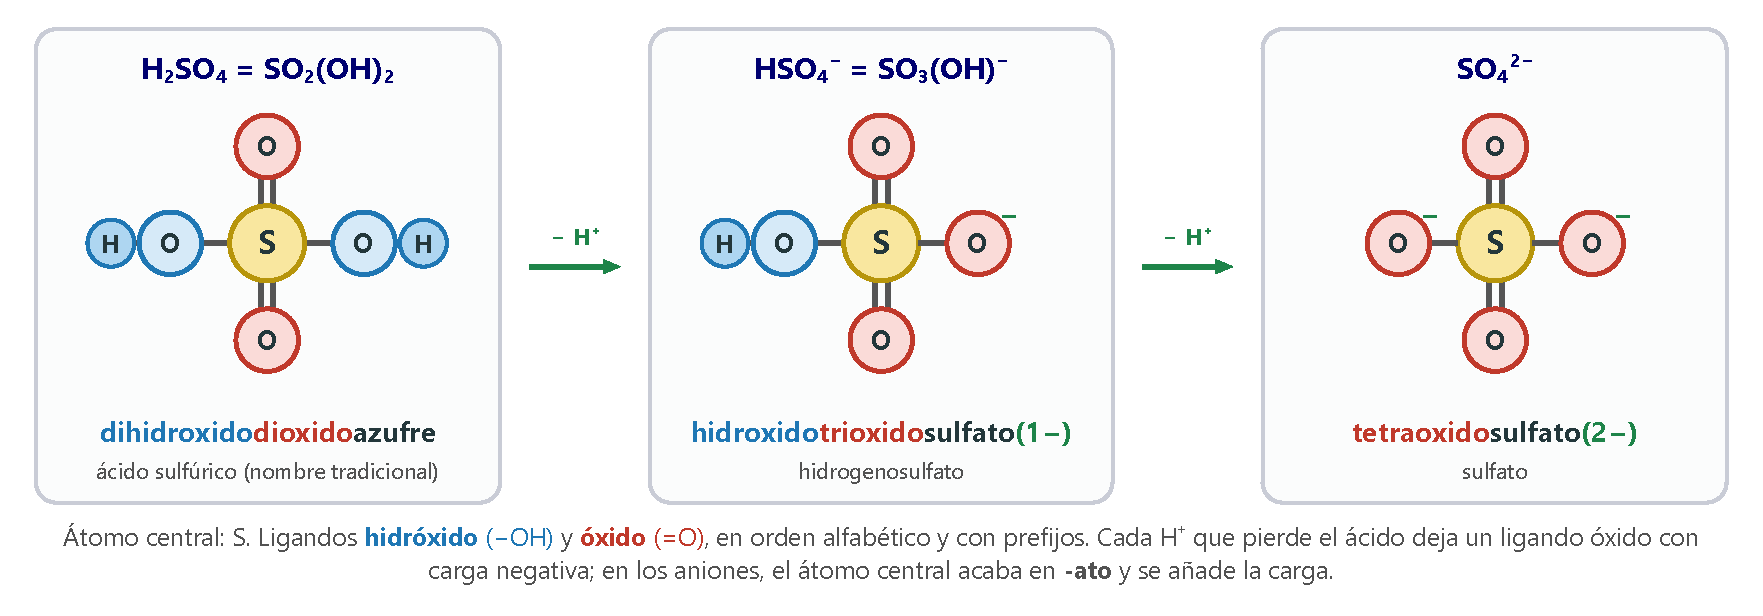
\includegraphics[width=\textwidth]{images/UD5/adicion_oxoacido}
    \caption{Nomenclatura de adición del ácido sulfúrico y de los aniones que se forman cuando pierde sus iones \ch{H+}.}
    \label{fig:ud5-adicion}
\end{figure}

\begin{table}[H]
    \centering
    \caption{Nombres de algunos oxoácidos en los tres sistemas}
    \vspace{-5pt}
    \small
    \setlength{\tabcolsep}{5pt}
    \begin{tabular}{@{}llL{4.35cm}L{4.1cm}@{}}
        \toprule
        \textbf{Fórmula} & \textbf{Tradicional} & \textbf{Hidrógeno} & \textbf{Adición} \\
        \midrule
        \ch{H3BO3} \(=\) \ch{B(OH)3} & ácido bórico & trihidrogeno(trioxidoborato) & trihidroxidoboro \\[3pt]
        \ch{H2CO3} \(=\) \ch{CO(OH)2} & ácido carbónico & dihidrogeno(trioxidocarbonato) & dihidroxidooxidocarbono \\[3pt]
        \ch{HNO2} \(=\) \ch{NO(OH)} & ácido nitroso & hidrogeno(dioxidonitrato) & hidroxidooxidonitrógeno \\[3pt]
        \ch{H3PO4} \(=\) \ch{PO(OH)3} & ácido fosfórico & trihidrogeno(tetraoxidofosfato) & trihidroxidooxidofósforo \\[3pt]
        \ch{H2SO4} \(=\) \ch{SO2(OH)2} & ácido sulfúrico & dihidrogeno(tetraoxidosulfato) & dihidroxidodioxidoazufre \\[3pt]
        \ch{HClO} \(=\) \ch{Cl(OH)} & ácido hipocloroso & hidrogeno(oxidoclorato) & hidroxidocloro \\[3pt]
        \ch{HIO3} \(=\) \ch{IO2(OH)} & ácido yódico & hidrogeno(trioxidoyodato) & hidroxidodioxidoyodo \\
        \bottomrule
    \end{tabular}
    \label{tab:ud5-oxoacidos-nombres}
\end{table}

\begin{example}
    \textbf{Oxoácidos.} a) Nombra el \ch{HBrO2} y el \ch{H4SiO4} en los tres sistemas. b) Formula el
    hidrogeno(tetraoxidomanganato) y el dihidroxidodioxidoselenio.

    \textbf{Solución.} a) \ch{HBrO2}: en la nomenclatura de hidrógeno, 1 H, 2 O y 1 Br: hidrogeno(dioxidobromato). Para la de
    adición se reescribe como \ch{BrO(OH)}: hidroxidooxidobromo. El estado de oxidación del Br es \(1 + x - 4 = 0\), \(x = +3\),
    el segundo de sus cuatro estados positivos: ácido \textbf{bromoso}.

    \ch{H4SiO4}: tetrahidrogeno(tetraoxidosilicato); \ch{Si(OH)4}, tetrahidroxidosilicio; ácido silícico.

    b) Hidrogeno(tetraoxidomanganato): 1 H, 4 O y 1 Mn: \ch{HMnO4} (ácido permangánico). Dihidroxidodioxidoselenio:
    \ch{SeO2(OH)2}, es decir, 2 H, 1 Se y 4 O: \ch{H2SeO4} (ácido selénico).
\end{example}

\begin{exercise}
    Nombra con la nomenclatura de hidrógeno y con la de adición, y da el nombre tradicional: a) \ch{HNO3}; b) \ch{H2SO3}; c)
    \ch{HClO4}; d) \ch{H3AsO4}; e) \ch{HIO}; f) \ch{H2TeO4}; g) \ch{HBrO3}; h) \ch{H3PO3}.
    \begin{solu}
        a) \textcolor{red}{hidrogeno(trioxidonitrato); \ch{NO2(OH)}, hidroxidodioxidonitrógeno; ácido nítrico}.
        b) \textcolor{red}{dihidrogeno(trioxidosulfato); \ch{SO(OH)2}, dihidroxidooxidoazufre; ácido sulfuroso}.
        c) \textcolor{red}{hidrogeno(tetraoxidoclorato); \ch{ClO3(OH)}, hidroxidotrioxidocloro; ácido perclórico}.
        d) \textcolor{red}{trihidrogeno(tetraoxidoarseniato); \ch{AsO(OH)3}, trihidroxidooxidoarsénico; ácido arsénico}.
        e) \textcolor{red}{hidrogeno(oxidoyodato); \ch{I(OH)}, hidroxidoyodo; ácido hipoyodoso}.
        f) \textcolor{red}{dihidrogeno(tetraoxidotelurato); \ch{TeO2(OH)2}, dihidroxidodioxidoteluro; ácido telúrico}.
        g) \textcolor{red}{hidrogeno(trioxidobromato); \ch{BrO2(OH)}, hidroxidodioxidobromo; ácido brómico}.
        h) \textcolor{red}{trihidrogeno(trioxidofosfato); \ch{P(OH)3}, trihidroxidofósforo; ácido fosforoso}.
    \end{solu}
\end{exercise}

\begin{exercise}
    Formula: a) hidrogeno(dioxidoclorato); b) dihidrogeno(trioxidocarbonato); c) trihidrogeno(tetraoxidofosfato); d)
    dihidrogeno(tetraoxidocromato); e) hidroxidodioxidocloro; f) tetrahidroxidosilicio; g) dihidroxidooxidoselenio; h)
    hidroxidotrioxidoyodo; i) ácido nitroso; j) ácido disulfúrico.
    \begin{solu}
        a) \textcolor{red}{\ch{HClO2}}; b) \textcolor{red}{\ch{H2CO3}}; c) \textcolor{red}{\ch{H3PO4}}; d)
        \textcolor{red}{\ch{H2CrO4}}; e) \textcolor{red}{\ch{HClO3}}; f) \textcolor{red}{\ch{H4SiO4}}; g)
        \textcolor{red}{\ch{H2SeO3}}; h) \textcolor{red}{\ch{HIO4}}; i) \textcolor{red}{\ch{HNO2}}; j)
        \textcolor{red}{\ch{H2S2O7}}.
    \end{solu}
\end{exercise}

\subsection{Oxoaniones}\label{sec:ud5-oxoaniones}

\begin{definition}[Oxoanión]
    Es el anión que queda cuando un oxoácido \textbf{pierde} uno o varios \textbf{iones \ch{H+}}. Tiene tantas \textbf{cargas
    negativas} como iones \ch{H+} ha perdido.
\end{definition}

El ácido carbónico, \ch{H2CO3}, puede perder sus dos \ch{H+} y dar el ion \ch{CO3^2-}, o perder solo uno y dar el
\ch{HCO3-}. Los oxoaniones que conservan algún hidrógeno se llaman \textbf{oxoaniones ácidos}.

\paragraph{Nombres tradicionales.} La IUPAC los admite para los oxoaniones que proceden de los ácidos de la
tabla~\ref{tab:ud5-oxoacidos}. Se cambia la terminación del ácido: \textbf{-oso} pasa a \textbf{-ito} e \textbf{-ico} pasa a
\textbf{-ato}, y se quita la palabra «ácido». Si quedan hidrógenos, se indica cuántos con el prefijo \textbf{hidrogeno}:
\begin{itemize}
    \item \ch{ClO-}, del ácido hipocloroso: \textbf{hipoclorito}. \ch{NO3-}, del ácido nítrico: \textbf{nitrato}.
    \ch{S2O7^2-}, del ácido disulfúrico: \textbf{disulfato}.
    \item \ch{H2PO4-}, del ácido fosfórico, que ha perdido un \ch{H+} y conserva dos: \textbf{dihidrogenofosfato}.
    \item Conviene conocer también \ch{CrO4^2-}, \textbf{cromato}; \ch{Cr2O7^2-}, \textbf{dicromato}; \ch{MnO4^2-},
    \textbf{manganato}, y \ch{MnO4-}, \textbf{permanganato}.
\end{itemize}

\paragraph{Nomenclatura de composición.} Se nombran los oxígenos con su prefijo, «oxido», la raíz del elemento central
terminada en \textbf{-ato} y el número de carga: \ch{SO4^2-} es el \textbf{tetraoxidosulfato(2\nobreakdash--)} y \ch{Cr2O7^2-}, el
\textbf{heptaoxidodicromato(2\nobreakdash--)}. Formular es inmediato a partir del nombre.

\paragraph{Nomenclatura de hidrógeno.} Solo se usa en los \textbf{oxoaniones ácidos}: se antepone el prefijo hidrogeno al nombre
de composición entre paréntesis y se añade la carga: \ch{H2PO4-} es el \textbf{dihidrogeno(tetraoxidofosfato)(1\nobreakdash--)}.

\paragraph{Nomenclatura de adición.} Se construye como en los oxoácidos, pero el átomo central termina en \textbf{-ato} y se
añade el número de carga: \ch{HSO3-} \(=\) \ch{SO2(OH)-} es el \textbf{hidroxidodioxidosulfato(1\nobreakdash--)}. Si el oxoanión no tiene
hidrógeno, el nombre coincide con el de composición (figura~\ref{fig:ud5-adicion}).

\begin{table}[H]
    \centering
    \caption{Nombres de algunos oxoaniones}
    \vspace{-5pt}
    \small
    \begin{tabular}{@{}lL{3.0cm}L{4.9cm}L{4.5cm}@{}}
        \toprule
        \textbf{Fórmula} & \textbf{Tradicional} & \textbf{Composición o hidrógeno} & \textbf{Adición} \\
        \midrule
        \ch{NO2-} & nitrito & dioxidonitrato(1\nobreakdash--) & dioxidonitrato(1\nobreakdash--) \\[3pt]
        \ch{CO3^2-} & carbonato & trioxidocarbonato(2\nobreakdash--) & trioxidocarbonato(2\nobreakdash--) \\[3pt]
        \ch{PO4^3-} & fosfato & tetraoxidofosfato(3\nobreakdash--) & tetraoxidofosfato(3\nobreakdash--) \\[3pt]
        \ch{ClO3-} & clorato & trioxidoclorato(1\nobreakdash--) & trioxidoclorato(1\nobreakdash--) \\[3pt]
        \ch{HCO3-} & hidrogenocarbonato & hidrogeno(trioxidocarbonato)(1\nobreakdash--) & hidroxidodioxidocarbonato(1\nobreakdash--) \\[3pt]
        \ch{HPO4^2-} & hidrogenofosfato & hidrogeno(tetraoxidofosfato)(2\nobreakdash--) & hidroxidotrioxidofosfato(2\nobreakdash--) \\[3pt]
        \ch{H2PO4-} & dihidrogenofosfato & dihidrogeno(tetraoxidofosfato)(1\nobreakdash--) & dihidroxidodioxidofosfato(1\nobreakdash--) \\[3pt]
        \ch{HSO4-} & hidrogenosulfato & hidrogeno(tetraoxidosulfato)(1\nobreakdash--) & hidroxidotrioxidosulfato(1\nobreakdash--) \\
        \bottomrule
    \end{tabular}
    \label{tab:ud5-oxoaniones}
\end{table}

\begin{example}
    \textbf{Oxoaniones.} a) ¿Qué oxoaniones puede formar el ácido sulfuroso? Nómbralos. b) Formula el ion
    trioxidoarseniato(3\nobreakdash--) y el hidroxidotrioxidofosfato(2\nobreakdash--).

    \textbf{Solución.} a) El \ch{H2SO3} puede perder un \ch{H+}: \ch{HSO3-}, hidrogenosulfito; hidrogeno(trioxidosulfato)(1\nobreakdash--);
    \ch{SO2(OH)-}, hidroxidodioxidosulfato(1\nobreakdash--). O los dos: \ch{SO3^2-}, sulfito; trioxidosulfato(2\nobreakdash--).

    b) Trioxidoarseniato(3\nobreakdash--): 3 O y 1 As con carga \(-3\): \ch{AsO3^3-} (arsenito, del ácido arsenoso).
    Hidroxidotrioxidofosfato(2\nobreakdash--): un ligando \ch{OH} y tres óxido unidos a un fósforo, \ch{PO3(OH)^2-}; reagrupando,
    \ch{HPO4^2-} (hidrogenofosfato). Comprobamos el estado de oxidación del P: \(1 + x - 8 = -2\), \(x = +5\), el mismo que en
    el ácido fosfórico.
\end{example}

\begin{exercise}
    Nombra con la nomenclatura de composición (o de hidrógeno, si tienen H) y da el nombre tradicional: a) \ch{SO3^2-}; b)
    \ch{BrO-}; c) \ch{IO4-}; d) \ch{SiO4^4-}; e) \ch{SeO4^2-}; f) \ch{BO3^3-}; g) \ch{HSeO4-}; h) \ch{H2AsO4-}; i) \ch{HCO3-};
    j) \ch{HPO4^2-}.
    \begin{solu}
        a) \textcolor{red}{trioxidosulfato(2\nobreakdash--); sulfito}. b) \textcolor{red}{oxidobromato(1\nobreakdash--); hipobromito}. c)
        \textcolor{red}{tetraoxidoyodato(1\nobreakdash--); peryodato}. d) \textcolor{red}{tetraoxidosilicato(4\nobreakdash--); silicato}. e)
        \textcolor{red}{tetraoxidoseleniato(2\nobreakdash--); seleniato}. f) \textcolor{red}{trioxidoborato(3\nobreakdash--); borato}. g)
        \textcolor{red}{hidrogeno(tetraoxidoseleniato)(1\nobreakdash--); hidrogenoseleniato}. h)
        \textcolor{red}{dihidrogeno(tetraoxidoarseniato)(1\nobreakdash--); dihidrogenoarseniato}. i)
        \textcolor{red}{hidrogeno(trioxidocarbonato)(1\nobreakdash--); hidrogenocarbonato}. j)
        \textcolor{red}{hidrogeno(tetraoxidofosfato)(2\nobreakdash--); hidrogenofosfato}.
    \end{solu}
\end{exercise}

\begin{exercise}
    a) Nombra con la nomenclatura de adición: \ch{HSO4-}, \ch{H2PO4-}, \ch{HCO3-}, \ch{HSeO3-}. b) Formula: trioxidonitrato(1\nobreakdash--),
    tetraoxidomanganato(1\nobreakdash--), dioxidoclorato(1\nobreakdash--), heptaoxidodicromato(2\nobreakdash--), hidrogeno(trioxidosulfato)(1\nobreakdash--), perclorato,
    cromato, hidroxidodioxidoarseniato(2\nobreakdash--).
    \begin{solu}
        a) \ch{SO3(OH)-}: \textcolor{red}{hidroxidotrioxidosulfato(1\nobreakdash--)}; \ch{PO2(OH)2-}: \textcolor{red}{dihidroxidodioxidofosfato(1\nobreakdash--)};
        \ch{CO2(OH)-}: \textcolor{red}{hidroxidodioxidocarbonato(1\nobreakdash--)}; \ch{SeO2(OH)-}:
        \textcolor{red}{hidroxidodioxidoseleniato(1\nobreakdash--)}. b) \textcolor{red}{\ch{NO3-}, \ch{MnO4-}, \ch{ClO2-}, \ch{Cr2O7^2-},
        \ch{HSO3-}, \ch{ClO4-}, \ch{CrO4^2-}}, \ch{AsO2(OH)^2-} \(=\) \textcolor{red}{\ch{HAsO3^2-}}.
    \end{solu}
\end{exercise}

\subsection{Oxosales}\label{sec:ud5-oxosales}

\begin{definition}[Oxosal]
    Es un compuesto formado por un \textbf{catión} y un \textbf{oxoanión}, combinados en la proporción necesaria para que el
    compuesto sea \textbf{neutro}.
\end{definition}

Para formular, se escribe el catión seguido del anión, con los números de cada uno como subíndices; el anión (y el catión, si es
poliatómico) va entre paréntesis si su subíndice es mayor que 1. Se nombra primero el anión y después el catión, como en un
compuesto binario. Para manejar las oxosales es imprescindible dominar antes los oxoaniones.

\paragraph{Nombre tradicional.} Se nombra el anión con su nombre tradicional y el catión con su número de oxidación (o de
carga) si tiene más de uno: sulfato de hierro(III).
\begin{itemize}
    \item \textbf{Formular}: sulfato de hierro(III). El anión es \ch{SO4^2-} y el catión, \ch{Fe^3+}. El mínimo común múltiplo
    de las cargas (2 y 3) es 6: hacen falta \textbf{3 aniones} y \textbf{2 cationes}: \ch{Fe2(SO4)3}.
    \item \textbf{Nombrar}: se separan catión y anión y se averigua la carga de cada uno. En el \ch{Fe2(SO4)3} hay 2 cationes y
    3 aniones; como las cargas totales tienen que ser iguales (6), cada anión tiene carga \(-2\) y cada catión, \(+3\).
\end{itemize}

No siempre es tan inmediato. En el \ch{CuBrO3}, el catión podría ser \ch{Cu+} o \ch{Cu^2+}. Si fuera \ch{Cu^2+}, el anión
sería \ch{BrO3^2-} y el bromo tendría \(x - 6 = -2\), \(x = +4\), que no es un estado de oxidación del bromo. Con \ch{Cu+} el
anión es \ch{BrO3-} (\(x = +5\), correcto): la sal es el \textbf{bromato de cobre(I)}.

\paragraph{Nomenclatura de composición.} La proporción se indica con prefijos multiplicadores; para el anión, que ya lleva
prefijos, se usan los \textbf{complejos} (bis, tris…) y su nombre va entre paréntesis: \ch{Ca(PO3)2} es el
bis(trioxidofosfato) de calcio, y el tris(tetraoxidosulfato) de dioro es \ch{Au2(SO4)3}.

\paragraph{Nomenclatura de adición.} Se nombran el anión y el catión con sus números de carga, sin indicar la proporción: el
\ch{K2Cr2O7} es el heptaoxidodicromato(2\nobreakdash--) de potasio. Para formular hay que calcular los subíndices, sabiendo que el compuesto
es neutro (dos \ch{K+} por cada \ch{Cr2O7^2-}). Para nombrar, primero hay que averiguar las cargas: en el \ch{FeSO4}, si el
catión fuera \ch{Fe^3+}, el anión sería \ch{SO4^3-} y el azufre tendría \(+5\), que no es válido; el catión es \ch{Fe^2+} y la
sal es el tetraoxidosulfato(2\nobreakdash--) de hierro(2+).

\begin{table}[H]
    \centering
    \caption{Nombres de algunas oxosales}
    \vspace{-5pt}
    \small
    \begin{tabular}{@{}lL{3.2cm}L{4.2cm}L{4.6cm}@{}}
        \toprule
        \textbf{Fórmula} & \textbf{Tradicional} & \textbf{Composición} & \textbf{Adición} \\
        \midrule
        \ch{NaClO} & hipoclorito de sodio & oxidoclorato de sodio & oxidoclorato(1\nobreakdash--) de sodio \\[3pt]
        \ch{CaCO3} & carbonato de calcio & trioxidocarbonato de calcio & trioxidocarbonato(2\nobreakdash--) de calcio \\[3pt]
        \ch{Fe2(SO4)3} & sulfato de hierro(III) & tris(tetraoxidosulfato) de dihierro & tetraoxidosulfato(2\nobreakdash--) de hierro(3+) \\[3pt]
        \ch{Ca3(PO4)2} & fosfato de calcio & bis(tetraoxidofosfato) de tricalcio & tetraoxidofosfato(3\nobreakdash--) de calcio \\[3pt]
        \ch{Pb(NO3)4} & nitrato de plomo(IV) & tetrakis(trioxidonitrato) de plomo & trioxidonitrato(1\nobreakdash--) de plomo(4+) \\[3pt]
        \ch{KMnO4} & permanganato de potasio & tetraoxidomanganato de potasio & tetraoxidomanganato(1\nobreakdash--) de potasio \\
        \bottomrule
    \end{tabular}
    \label{tab:ud5-oxosales}
\end{table}

\begin{example}
    \textbf{Oxosales.} a) Nombra el \ch{Pb(CO3)2} en los tres sistemas. b) Formula el clorito de aluminio y el
    bis(tetraoxidoclorato) de cobre.

    \textbf{Solución.} a) Hay 2 aniones \ch{CO3}. Si el catión fuera \ch{Pb^2+}, cada anión sería \ch{CO3-} y el carbono tendría
    \(x - 6 = -1\), \(x = +5\): imposible. El anión es \ch{CO3^2-} (carbonato) y el catión, \ch{Pb^4+}. Nombres: carbonato de
    plomo(IV); bis(trioxidocarbonato) de plomo; trioxidocarbonato(2\nobreakdash--) de plomo(4+).

    b) Clorito: \ch{ClO2-} (del ácido cloroso); aluminio: \ch{Al^3+}. Hacen falta 3 aniones por cada catión: \ch{Al(ClO2)3}.
    Bis(tetraoxidoclorato) de cobre: dos aniones \ch{ClO4-} y un cobre: \ch{Cu(ClO4)2}.
\end{example}

\begin{exercise}
    Determina las cargas del catión y del anión y da el nombre tradicional de: a) \ch{NaNO2}; b) \ch{Fe(NO3)3}; c) \ch{Hg2SO4};
    d) \ch{K2CrO4}; e) \ch{Al2(SO3)3}; f) \ch{Mg3(PO4)2}; g) \ch{Cu(IO3)2}; h) \ch{Ba(MnO4)2}.
    \begin{solu}
        a) \ch{Na+} y \ch{NO2-}: \textcolor{red}{nitrito de sodio}. b) \ch{Fe^3+} y \ch{NO3-}: \textcolor{red}{nitrato de
        hierro(III)}. c) \ch{Hg2^2+} (o \ch{Hg+}) y \ch{SO4^2-}: \textcolor{red}{sulfato de mercurio(I)}. d) \ch{K+} y \ch{CrO4^2-}:
        \textcolor{red}{cromato de potasio}. e) \ch{Al^3+} y \ch{SO3^2-}: \textcolor{red}{sulfito de aluminio}. f) \ch{Mg^2+} y
        \ch{PO4^3-}: \textcolor{red}{fosfato de magnesio}. g) \ch{Cu^2+} y \ch{IO3-}: \textcolor{red}{yodato de cobre(II)}.
        h) \ch{Ba^2+} y \ch{MnO4-}: \textcolor{red}{permanganato de bario}.
    \end{solu}
\end{exercise}

\begin{exercise}
    a) Nombra con la nomenclatura de composición y con la de adición: \ch{Na2SO4}, \ch{Ni(ClO3)2}, \ch{Al(NO3)3},
    \ch{Co2(CO3)3}. b) Formula: carbonato de sodio, nitrato de plata, perclorato de potasio, sulfato de cobre(II), fosfato de
    hierro(II), bis(trioxidonitrato) de calcio, tris(tetraoxidosulfato) de dicromo, tetraoxidomanganato(1\nobreakdash--) de sodio,
    trioxidoyodato(1\nobreakdash--) de plomo(2+).
    \begin{solu}
        a) \textcolor{red}{tetraoxidosulfato de disodio; tetraoxidosulfato(2\nobreakdash--) de sodio}. \textcolor{red}{bis(trioxidoclorato) de
        níquel; trioxidoclorato(1\nobreakdash--) de níquel(2+)}. \textcolor{red}{tris(trioxidonitrato) de aluminio; trioxidonitrato(1\nobreakdash--) de
        aluminio}. \textcolor{red}{tris(trioxidocarbonato) de dicobalto; trioxidocarbonato(2\nobreakdash--) de cobalto(3+)}.
        b) \textcolor{red}{\ch{Na2CO3}, \ch{AgNO3}, \ch{KClO4}, \ch{CuSO4}, \ch{Fe3(PO4)2}, \ch{Ca(NO3)2}, \ch{Cr2(SO4)3},
        \ch{NaMnO4}, \ch{Pb(IO3)2}}.
    \end{solu}
\end{exercise}

\subsection{Sales ácidas}\label{sec:ud5-sales-acidas}

\paragraph{Sales ácidas de oxoácidos.} Están formadas por un catión y un \textbf{oxoanión ácido}, que procede de un oxoácido que
no ha perdido todos sus hidrógenos. Todo lo dicho para las oxosales es válido; solo hay que saber nombrar y formular el anión.

\paragraph{Sales ácidas de haluros de hidrógeno.} Las disoluciones de \ch{H2S}, \ch{H2Se} y \ch{H2Te} son ácidas. Si pierden solo
uno de sus dos \ch{H+}, quedan los aniones \ch{HS-}, \ch{HSe-} y \ch{HTe-}, que forman sales con los cationes: \ch{KHS} es el
hidrogenosulfuro de potasio o hidrogeno(sulfuro) de potasio. Los haluros del grupo 17 (\ch{HCl}…) solo tienen un hidrógeno y no
forman sales ácidas.

\begin{table}[H]
    \centering
    \caption{Nombres de algunas sales ácidas}
    \vspace{-5pt}
    \begin{tabular}{@{}lllL{3.6cm}L{5.4cm}@{}}
        \toprule
        \textbf{Fórmula} & \textbf{Catión} & \textbf{Anión} & \textbf{Tradicional} & \textbf{Composición} \\
        \midrule
        \ch{NaHSO4} & \ch{Na+} & \ch{HSO4-} & hidrogenosulfato de sodio & hidrogeno(tetraoxidosulfato) de sodio \\[3pt]
        \ch{Ca(HCO3)2} & \ch{Ca^2+} & \ch{HCO3-} & hidrogenocarbonato de calcio & bis[hidrogeno(trioxidocarbonato)] de calcio \\[3pt]
        \ch{KH2PO4} & \ch{K+} & \ch{H2PO4-} & dihidrogenofosfato de potasio & dihidrogeno(tetraoxidofosfato) de potasio \\[3pt]
        \ch{Fe(HS)2} & \ch{Fe^2+} & \ch{HS-} & hidrogenosulfuro de hierro(II) & bis[hidrogeno(sulfuro)] de hierro \\[3pt]
        \ch{NH4HSe} & \ch{NH4+} & \ch{HSe-} & hidrogenoseleniuro de amonio & hidrogeno(seleniuro) de amonio \\
        \bottomrule
    \end{tabular}
    \label{tab:ud5-sales-acidas}
\end{table}

Fíjate en que, cuando el nombre del anión ya lleva paréntesis y hay que multiplicarlo, se usan \textbf{corchetes}:
bis[hidrogeno(trioxidocarbonato)]. El hidrogenocarbonato de sodio, \ch{NaHCO3}, es el «bicarbonato» de la cocina; el
nombre bicarbonato no es aceptado por la IUPAC.

\begin{exercise}
    a) Nombra: \ch{KHCO3}, \ch{Mg(HSO4)2}, \ch{Na2HPO4}, \ch{LiH2PO4}, \ch{Ba(HS)2}, \ch{CuHSO3}, \ch{NaHSe}, \ch{Fe(HCO3)3}. b)
    Formula: hidrogenocarbonato de magnesio, hidrogenosulfato de potasio, dihidrogenofosfato de calcio, hidrogenosulfuro de
    sodio, hidrogeno(tetraoxidosulfato) de plata, hidrogenosulfito de aluminio, hidrogenotelururo de cobre(II).
    \begin{solu}
        a) \textcolor{red}{hidrogenocarbonato de potasio}; \textcolor{red}{hidrogenosulfato de magnesio}; \textcolor{red}{hidrogenofosfato
        de sodio}; \textcolor{red}{dihidrogenofosfato de litio}; \textcolor{red}{hidrogenosulfuro de bario};
        \textcolor{red}{hidrogenosulfito de cobre(I)}; \textcolor{red}{hidrogenoseleniuro de sodio};
        \textcolor{red}{hidrogenocarbonato de hierro(III)}. b) \textcolor{red}{\ch{Mg(HCO3)2}, \ch{KHSO4}, \ch{Ca(H2PO4)2},
        \ch{NaHS}, \ch{AgHSO4}, \ch{Al(HSO3)3}, \ch{Cu(HTe)2}}.
    \end{solu}
\end{exercise}

\subsection{Sales hidratadas}\label{sec:ud5-hidratadas}

\begin{definition}[Sal hidratada]
    Es una sal que contiene moléculas de \textbf{agua} en su estructura cristalina, en una proporción fija. En la fórmula, las
    moléculas de agua se escriben detrás de un punto centrado: \ch{CuSO4 * 5 H2O}.
\end{definition}

Se nombra la sal por cualquiera de los sistemas válidos, seguida de «agua» y, entre paréntesis, la proporción sal/agua; o bien
se añade la palabra hidrato con el prefijo multiplicador correspondiente:
\begin{itemize}
    \item \ch{Na2CO3 * 10 H2O}: carbonato de sodio---agua (1/10) o carbonato de sodio decahidrato.
    \item \ch{FeCl3 * 6 H2O}: tricloruro de hierro---agua (1/6) o tricloruro de hierro hexahidrato.
    \item \ch{3 CdSO4 * 8 H2O}: sulfato de cadmio---agua (3/8). Aquí solo sirve la primera forma, porque la proporción no es un
    número entero de moléculas de agua por cada unidad de sal.
\end{itemize}
Al calentarlas, estas sales pierden el agua: el sulfato de cobre(II) pentahidrato, azul, se vuelve blanco al deshidratarse
(práctica de la sección~\ref{sec:ud5-practicas}).

\begin{exercise}
    a) Nombra: \ch{MgSO4 * 7 H2O}, \ch{CaCl2 * 2 H2O}, \ch{CoCl2 * 6 H2O}, \ch{Na2SO4 * 10 H2O}. b) Formula: sulfato de calcio
    dihidrato, cloruro de bario---agua (1/2), nitrato de níquel(II) hexahidrato, carbonato de sodio---agua (1/1).
    \begin{solu}
        a) \textcolor{red}{sulfato de magnesio heptahidrato} (sulfato de magnesio---agua (1/7)); \textcolor{red}{cloruro de
        calcio dihidrato}; \textcolor{red}{cloruro de cobalto(II) hexahidrato}; \textcolor{red}{sulfato de sodio decahidrato}.
        b) \textcolor{red}{\ch{CaSO4 * 2 H2O}, \ch{BaCl2 * 2 H2O}, \ch{Ni(NO3)2 * 6 H2O}, \ch{Na2CO3 * H2O}}.
    \end{solu}
\end{exercise}

\begin{exercise}
    El yeso es sulfato de calcio dihidrato. a) Escribe su fórmula. b) ¿Qué porcentaje de su masa es agua?
    (\(M(\ch{Ca}) = 40{,}1\), \(M(\ch{S}) = 32{,}1\), \(M(\ch{O}) = 16{,}0\), \(M(\ch{H}) = 1{,}0\) en \unit{\gram\per\mol}).
    \begin{solu}
        a) \textcolor{red}{\ch{CaSO4 * 2 H2O}}. b) \(M(\ch{CaSO4}) = 40{,}1 + 32{,}1 + 64{,}0 = \qty{136.2}{\gram\per\mol}\);
        \(M(2\,\ch{H2O}) = \qty{36.0}{\gram\per\mol}\); \(M = \qty{172.2}{\gram\per\mol}\).
        \(\dfrac{36{,}0}{172{,}2} \cdot 100 = \textcolor{red}{\qty{20.9}{\percent}}\).
    \end{solu}
\end{exercise}

%========================================================================================
\section{Química en la vida: de la alquimia a la IUPAC}\label{sec:ud5-historia}
%========================================================================================

Hasta finales del siglo \textsc{xviii}, cada sustancia tenía un nombre heredado de la alquimia, del comercio o de la farmacia:
aceite de vitriolo (ácido sulfúrico), espíritu de sal (ácido clorhídrico), sal de Glauber (sulfato de sodio decahidrato), flores
de cinc (óxido de cinc)\dots{} Un mismo compuesto podía tener varios nombres y un mismo nombre servir para sustancias distintas.

En 1787, cuatro químicos franceses, \textbf{Guyton de Morveau}, \textbf{Lavoisier}, \textbf{Berthollet} y \textbf{Fourcroy},
publicaron el \textit{Método de nomenclatura química}. Su idea era revolucionaria: el nombre de un compuesto debía indicar
\textbf{de qué está hecho}. De ahí vienen los óxidos, los sulfatos o los nitratos, y las terminaciones -oso e -ico para
distinguir la «cantidad de oxígeno». Poco después, \textbf{Berzelius} propuso escribir los elementos con una o dos letras de su
nombre latino, que es el origen de nuestros símbolos (Na de \textit{natrium}, Fe de \textit{ferrum}, S de \textit{sulphur}).

El número de compuestos conocidos no dejó de crecer, y en el siglo \textsc{xx} se hizo necesario un organismo internacional que
pusiera orden: la IUPAC, fundada en 1919, publica periódicamente sus recomendaciones, conocidas por el color de las tapas. El
\textbf{Libro Rojo} recoge la nomenclatura inorgánica; su versión vigente es de 2005. Muchos nombres que aprendieron tus padres
(anhídridos, ácido sulfhídrico, bicarbonato) ya no se recomiendan, y otros nuevos, como dihidrogeno(tetraoxidosulfato), se
basan en la estructura de las moléculas. La química sigue cambiando, y su lenguaje también.

\begin{exercise}
    a) ¿Qué principio introdujo el \textit{Método de nomenclatura química} de 1787? b) La sal de Glauber es sulfato de sodio
    decahidrato y el aceite de vitriolo, ácido sulfúrico. Escribe sus fórmulas. c) ¿Por qué el nombre «bicarbonato» no indica
    bien la composición del \ch{NaHCO3}?
    \begin{solu}
        a) \textcolor{red}{Que el nombre de un compuesto indique de qué elementos está formado.} b) \textcolor{red}{\ch{Na2SO4 *
        10 H2O} y \ch{H2SO4}}. c) \textcolor{red}{El prefijo bi- sugiere que hay dos carbonatos}, cuando en realidad la sal tiene
        un anión carbonato con un hidrógeno (\ch{HCO3-}); el nombre correcto es hidrogenocarbonato de sodio.
    \end{solu}
\end{exercise}

%========================================================================================
\section{Prácticas}\label{sec:ud5-practicas}
%========================================================================================

\subsection{Química en casa: la química de las etiquetas}

\noindent\begin{minipage}[t]{0.48\textwidth}
    \textbf{Objetivo}
    \begin{itemize}
        \item Identificar compuestos inorgánicos en las etiquetas de productos cotidianos, escribir su fórmula y nombrarlos
        correctamente.
    \end{itemize}
\end{minipage}\hfill
\begin{minipage}[t]{0.48\textwidth}
    \textbf{Material}
    \begin{itemize}
        \item Envases o fotografías de las etiquetas de productos de limpieza, de higiene, de alimentación y de jardinería:
        lejía, salfumán, pasta de dientes, sal yodada, bicarbonato, agua mineral, abono, productos para piscinas\dots
    \end{itemize}
\end{minipage}

\textbf{Procedimiento}
\begin{enumerate}[label=\numberballgreen]
    \item Busca en cada etiqueta la composición o los ingredientes y anota los compuestos inorgánicos que aparezcan.
    \item Para cada uno, escribe su fórmula, el tipo de compuesto y su nombre en al menos dos sistemas de nomenclatura.
    \item Señala los nombres de las etiquetas que no siguen las normas de la IUPAC y corrígelos.
    \item Anota los pictogramas de peligro de cada producto y las advertencias de uso.
\end{enumerate}
\textbf{No abras ni mezcles los productos: trabaja solo con las etiquetas.}

\begin{exercise}
    Algunos compuestos que suelen aparecer en las etiquetas son: hipoclorito de sodio (lejía), fluoruro de sodio (pasta de
    dientes), yoduro de potasio (sal yodada), «bicarbonato sódico», «cloruro magnésico» y «sulfato cálcico» (aguas minerales) y
    nitrato de amonio (abonos). a) Escribe sus fórmulas. b) Corrige los nombres que no siguen las normas de la IUPAC. c) ¿Qué tipo
    de compuesto es cada uno?
    \begin{solu}
        a) \textcolor{red}{\ch{NaClO}, \ch{NaF}, \ch{KI}, \ch{NaHCO3}, \ch{MgCl2}, \ch{CaSO4}, \ch{NH4NO3}}. b)
        \textcolor{red}{Hidrogenocarbonato de sodio, cloruro de magnesio y sulfato de calcio} (no se usan los adjetivos
        «sódico», «magnésico», «cálcico»). c) \textcolor{red}{\ch{NaF}, \ch{KI} y \ch{MgCl2}: sales binarias; \ch{NaClO},
        \ch{CaSO4} y \ch{NH4NO3}: oxosales; \ch{NaHCO3}: sal ácida.}
    \end{solu}
\end{exercise}

\subsection{¿Cuánta agua tiene una sal hidratada?}

\noindent\begin{minipage}[t]{0.48\textwidth}
    \textbf{Objetivo}
    \begin{itemize}
        \item Determinar experimentalmente el número de moléculas de agua de hidratación del sulfato de cobre(II).
    \end{itemize}
\end{minipage}\hfill
\begin{minipage}[t]{0.48\textwidth}
    \textbf{Material y reactivos}
    \begin{itemize}
        \item Crisol de porcelana (o cápsula), triángulo de arcilla, trípode, mechero, pinzas, desecador y balanza de
        precisión (\qty{0.01}{\gram}).
        \item Sulfato de cobre(II) hidratado (cristales azules) y unas gotas de agua.
    \end{itemize}
\end{minipage}

\textbf{Procedimiento}
\begin{enumerate}[label=\numberballgreen]
    \item Pesa el crisol limpio y seco (\(m_1\)). Añade unos \qty{2}{\gram} de sulfato de cobre hidratado, triturado, y pesa
    de nuevo (\(m_2\)).
    \item Calienta suavemente, removiendo con una varilla, hasta que todo el sólido pase de azul a blanco grisáceo. Evita
    calentar al rojo: el sulfato se descompondría.
    \item Deja enfriar el crisol en el desecador y pésalo (\(m_3\)). Calienta otra vez unos minutos y vuelve a pesar, hasta que
    la masa no cambie.
    \item Deja caer unas gotas de agua sobre el sólido blanco y observa qué ocurre.
\end{enumerate}
\textbf{Usa gafas y pinzas: el crisol quema. El sulfato de cobre es nocivo: lávate las manos al terminar.}

\begin{exercise}
    En una práctica se obtuvieron \(m_1 = \qty{24.36}{\gram}\), \(m_2 = \qty{26.41}{\gram}\) y \(m_3 = \qty{25.67}{\gram}\).
    a) Calcula la masa de sal anhidra y la de agua perdida. b) Calcula los moles de cada una y la fórmula de la sal hidratada
    (\(M(\ch{CuSO4}) = \qty{159.6}{\gram\per\mol}\)). c) Nombra la sal. d) ¿Qué ocurre al añadir agua al sólido blanco?
    \begin{solu}
        a) \(m(\ch{CuSO4}) = 25{,}67 - 24{,}36 = \textcolor{red}{\qty{1.31}{\gram}}\); \(m(\ch{H2O}) = 26{,}41 - 25{,}67 =
        \textcolor{red}{\qty{0.74}{\gram}}\). b) \(n(\ch{CuSO4}) = \dfrac{1{,}31}{159{,}6} = \qty{8.21e-3}{\mol}\);
        \(n(\ch{H2O}) = \dfrac{0{,}74}{18{,}0} = \qty{4.11e-2}{\mol}\). Relación: \(\dfrac{4{,}11 \cdot 10^{-2}}{8{,}21 \cdot
        10^{-3}} = 5{,}0\): \textcolor{red}{\ch{CuSO4 * 5 H2O}}. c) \textcolor{red}{Sulfato de cobre(II) pentahidrato}
        (tetraoxidosulfato de cobre---agua (1/5)). d) \textcolor{red}{El sólido vuelve a ponerse azul y se calienta}: la sal se
        hidrata de nuevo, desprendiendo energía.
    \end{solu}
\end{exercise}

%========================================================================================
\section{Situación de aprendizaje: productos de limpieza seguros (ODS 3)}\label{sec:ud5-ods}
%========================================================================================

Cada año, los servicios de información toxicológica atienden miles de consultas por intoxicaciones con productos de limpieza
domésticos. Muchas se deben a una costumbre peligrosa: \textbf{mezclar productos} pensando que así limpian más. Al mezclar lejía
(hipoclorito de sodio) con salfumán (cloruro de hidrógeno en disolución) se desprende \textbf{dicloro}, un gas tóxico; y al
mezclarla con limpiadores amoniacales se forman cloraminas, también irritantes. El \textbf{Objetivo de Desarrollo Sostenible 3}
(salud y bienestar) incluye reducir las muertes y enfermedades causadas por productos químicos peligrosos.

\begin{marker}
    \textbf{Reto:} elaborad una guía (cartel, folleto o vídeo) para las familias del centro sobre el uso seguro de los productos
    de limpieza, con el nombre correcto y la fórmula de sus componentes principales.
\end{marker}

\begin{enumerate}[label=\numberballred]
    \item \textbf{Investigad} la composición de los productos de limpieza más comunes (lejía, salfumán, amoniaco, desatascadores,
    lavavajillas, limpiacristales\dots) y escribid la fórmula y el nombre IUPAC de sus componentes inorgánicos.
    \item \textbf{Investigad} el significado de los pictogramas de peligro (reglamento CLP) y qué productos no deben mezclarse
    nunca y por qué.
    \item \textbf{Calculad.} a) La reacción entre la lejía y el salfumán es
    \ch{NaClO + 2 HCl -> NaCl + Cl2 + H2O}. Nombrad todas las sustancias. b) Una lejía tiene \qty{40}{\gram} de cloro activo por
    litro, que equivale a \qty{42}{\gram} de \ch{NaClO} por litro. Si se mezcla un vaso (\qty{200}{\milli\litre}) con salfumán
    en exceso, ¿cuántos moles de \ch{Cl2} se forman? ¿Qué volumen ocupan a \qty{20}{\degreeCelsius} y \qty{1}{\atm}?
    \item \textbf{Comunicad.} La guía debe incluir: los productos más habituales con su fórmula y su nombre correcto; las mezclas
    peligrosas y sus consecuencias; los pictogramas; qué hacer en caso de intoxicación (teléfono del Servicio de Información
    Toxicológica, 91 562 04 20), y alternativas más seguras y respetuosas con el medio ambiente.
\end{enumerate}

\begin{exercise}
    Resuelve los cálculos del apartado 3 de la situación de aprendizaje (\(M(\ch{NaClO}) = \qty{74.5}{\gram\per\mol}\),
    \(R = \qty{0.082}{\atm\litre\per\mol\per\kelvin}\)).
    \begin{solu}
        a) \textcolor{red}{Hipoclorito de sodio (oxidoclorato de sodio), cloruro de hidrógeno, cloruro de sodio, dicloro y agua.}
        b) \(m(\ch{NaClO}) = 42 \cdot 0{,}200 = \qty{8.4}{\gram}\); \(n = \dfrac{8{,}4}{74{,}5} = \qty{0.113}{\mol}\) de \ch{NaClO},
        que dan \textcolor{red}{\qty{0.113}{\mol} de \ch{Cl2}} (relación 1:1).
        \(V = \dfrac{nRT}{p} = \dfrac{0{,}113 \cdot 0{,}082 \cdot 293}{1} = \textcolor{red}{\qty{2.7}{\litre}}\) de un gas tóxico.
    \end{solu}
\end{exercise}

\fussy

    \newpage
    %! Unidad 5 — Nomenclatura de química inorgánica: ejercicios resueltos y ejercicios finales
%! Fuente: Fuentes/Quimica/Unidad 5 («Ejercicios», «Ejercicios resueltos» y «Practica y calcula»).
%! Enunciados adaptados con compuestos cambiados; soluciones rehechas. Dificultad: \(\star\) baja, \(\star\star\) media, \(\star\star\star\) alta.

\sloppy % nombres largos sin guiones: se permite más espacio entre palabras (\fussy al final)

\section{Ejercicios resueltos}\label{sec:ud5-resueltos}

\begin{example}
    \textbf{Identificar el tipo de compuesto.} Clasifica estas sustancias y nómbralas: \ch{Ba(OH)2}, \ch{N2O4}, \ch{HIO4},
    \ch{K2O2}, \ch{NH4Cl}, \ch{SbH3}.

    \textbf{Solución.} Para clasificar, mira primero cuántos elementos hay y qué hay a la derecha de la fórmula:
    \begin{itemize}
        \item \ch{Ba(OH)2}: metal y \ch{OH}: \textbf{hidróxido}. Hidróxido de bario (el bario solo tiene \(+2\)).
        \item \ch{N2O4}: binario con O a la derecha: \textbf{óxido}. Tetraóxido de dinitrógeno; óxido de nitrógeno(IV)
        (\(2x - 8 = 0\), \(x = +4\)). No se simplifica la fórmula: el \ch{N2O4} y el \ch{NO2} son sustancias distintas.
        \item \ch{HIO4}: H, un no metal y O: \textbf{oxoácido}. Ácido peryódico (I con \(+7\)); hidrogeno(tetraoxidoyodato);
        \ch{IO3(OH)}, hidroxidotrioxidoyodo.
        \item \ch{K2O2}: el K solo tiene \(+1\), así que cada O tiene \(-1\): \textbf{peróxido}. Peróxido de potasio; dióxido de
        dipotasio.
        \item \ch{NH4Cl}: catión amonio y anión cloruro: \textbf{sal}, aunque sea ternaria se nombra como una binaria. Cloruro de
        amonio.
        \item \ch{SbH3}: binario con H a la derecha: \textbf{hidruro}. Trihidruro de antimonio; hidruro de antimonio(III);
        estibano.
    \end{itemize}
\end{example}

\begin{example}
    \textbf{Formular a partir del número de oxidación.} Formula el óxido de cloro(VII), el sulfuro de plomo(IV), el hidróxido de
    hierro(II) y el peróxido de aluminio.

    \textbf{Solución.} En cada caso escribimos los iones (o los estados de oxidación) y aplicamos la regla de la suma:
    \begin{itemize}
        \item Óxido de cloro(VII): ¡cuidado!, el O aparece antes que el Cl en la secuencia, así que este compuesto es un haluro de
        oxígeno. Con Cl \(+7\) y O \(-2\) la proporción es 2:7: la fórmula es \ch{O7Cl2}, dicloruro de heptaoxígeno. El nombre
        «óxido de cloro(VII)» no es correcto.
        \item Sulfuro de plomo(IV): \ch{Pb^4+} y \ch{S^2-}: \ch{Pb2S4} \(\rightarrow\) \ch{PbS2}.
        \item Hidróxido de hierro(II): \ch{Fe^2+} y \ch{OH-}: \ch{Fe(OH)2}.
        \item Peróxido de aluminio: \ch{Al^3+} y \ch{O2^2-}. Con 2 Al y 3 \ch{O2^2-}: \ch{Al2(O2)3} \(=\) \ch{Al2O6}. Como es un
        peróxido, no se simplifica.
    \end{itemize}
\end{example}

\begin{example}
    \textbf{Nombrar un oxoácido «desconocido».} Nombra el \ch{H2MnO4} en las nomenclaturas de hidrógeno y de adición. ¿Qué
    estado de oxidación tiene el manganeso? ¿Cómo se llama el anión que se forma al perder sus dos \ch{H+}?

    \textbf{Solución.} \textbf{1. Hidrógeno}: 2 H, 4 O, 1 Mn: dihidrogeno(tetraoxidomanganato). \textbf{2. Adición}:
    \ch{MnO2(OH)2}, dihidroxidodioxidomanganeso. \textbf{3. Estado de oxidación}: \(2 + x - 8 = 0\), \(x = +6\).
    \textbf{4. Anión}: \ch{MnO4^2-}, tetraoxidomanganato(2\nobreakdash--), cuyo nombre tradicional es \textbf{manganato}. No lo confundas con
    el \ch{MnO4-}, permanganato (Mn \(+7\)).
\end{example}

\begin{example}
    \textbf{Nombrar una oxosal sin saber la carga del catión.} Nombra el \ch{Co(ClO2)3} y el \ch{NiSO3} en los tres sistemas.

    \textbf{Solución.} \textbf{\ch{Co(ClO2)3}}: hay 3 aniones \ch{ClO2}. Si su carga fuera \(-1\), el Cl tendría \(x - 4 = -1\),
    \(x = +3\), correcto, y el catión sería \ch{Co^3+}, también posible. Es el clorito de cobalto(III);
    tris(dioxidoclorato) de cobalto; dioxidoclorato(1\nobreakdash--) de cobalto(3+).

    \textbf{\ch{NiSO3}}: un catión y un anión. Si el anión fuera \ch{SO3^2-} (S con \(+4\)), el catión sería \ch{Ni^2+}, que es
    posible. Si fuera \ch{SO3^3-}, el S tendría \(+3\), que no es válido. Es el sulfito de níquel(II); trioxidosulfato de níquel;
    trioxidosulfato(2\nobreakdash--) de níquel(2+).
\end{example}

\begin{example}
    \textbf{Sales ácidas e hidratadas.} a) Formula el hidrogenofosfato de amonio y el bis[dihidrogeno(tetraoxidofosfato)] de
    magnesio. b) Nombra el \ch{Na2B4O7 * 10 H2O} (bórax), sabiendo que su anión es el heptaoxidotetraborato(2\nobreakdash--).

    \textbf{Solución.} a) Hidrogenofosfato: \ch{HPO4^2-}; amonio: \ch{NH4+}. Hacen falta dos amonios: \ch{(NH4)2HPO4}. Es un
    abono muy usado. El segundo tiene dos aniones \ch{H2PO4-} y un magnesio: \ch{Mg(H2PO4)2}.

    b) Heptaoxidotetraborato de disodio---agua (1/10), o heptaoxidotetraborato de disodio decahidrato.
\end{example}

%========================================================================================
\section{Ejercicios de aplicación}\label{sec:ud5-aplicacion}
%========================================================================================

\subsection{Conceptos previos}

\begin{exercise}
    \(\star\) Clasifica estas sustancias en simples, binarias, ternarias o cuaternarias: \ch{Cl2}, \ch{KNO3}, \ch{CaO}, \ch{NaHSO4},
    \ch{Fe}, \ch{H3PO4}, \ch{HBr}, \ch{NH4HCO3}, \ch{O3}, \ch{Mg(OH)2}.
    \begin{solu}
        \textcolor{red}{Simples}: \ch{Cl2}, \ch{Fe}, \ch{O3}. \textcolor{red}{Binarias}: \ch{CaO}, \ch{HBr}.
        \textcolor{red}{Ternarias}: \ch{KNO3}, \ch{H3PO4}, \ch{Mg(OH)2}. \textcolor{red}{Cuaternarias}: \ch{NaHSO4}, \ch{NH4HCO3}.
    \end{solu}
\end{exercise}

\begin{exercise}
    \(\star\star\) Calcula el estado de oxidación de cada elemento en: a) \ch{HNO2}; b) \ch{Na2CrO4}; c) \ch{Al2(SO4)3}; d)
    \ch{MnO4-}; e) \ch{H2O2}; f) \ch{CaH2}; g) \ch{NH3}; h) \ch{S2O3^2-}.
    \begin{solu}
        a) \textcolor{red}{H \(+1\), N \(+3\), O \(-2\)}. b) \textcolor{red}{Na \(+1\), Cr \(+6\), O \(-2\)}. c)
        \textcolor{red}{Al \(+3\), S \(+6\), O \(-2\)} (anión \ch{SO4^2-}). d) \textcolor{red}{Mn \(+7\), O \(-2\)}. e)
        \textcolor{red}{H \(+1\), O \(-1\)}. f) \textcolor{red}{Ca \(+2\), H \(-1\)}. g) \textcolor{red}{N \(-3\), H \(+1\)}.
        h) \(2x - 6 = -2\): \textcolor{red}{S \(+2\), O \(-2\)}.
    \end{solu}
\end{exercise}

\begin{exercise}
    \(\star\star\) Con la regla de la suma, decide si son posibles estos compuestos y corrige los que no lo sean: a) \ch{NaS};
    b) \ch{BaCl2}; c) \ch{AlO}; d) \ch{K3P}; e) \ch{MgN}; f) \ch{ZnBr}.
    \begin{solu}
        a) \textcolor{red}{No}: \(+1 - 2 = -1\); \textcolor{red}{\ch{Na2S}}. b) \textcolor{red}{Sí}. c) \textcolor{red}{No}:
        \(+3 - 2 \neq 0\); \textcolor{red}{\ch{Al2O3}}. d) \textcolor{red}{Sí}: \(3 - 3 = 0\). e) \textcolor{red}{No}:
        \(+2 - 3 \neq 0\); \textcolor{red}{\ch{Mg3N2}}. f) \textcolor{red}{No}; \textcolor{red}{\ch{ZnBr2}}.
    \end{solu}
\end{exercise}

\begin{exercise}
    \(\star\star\) Usando la secuencia de los elementos (figura~\ref{fig:ud5-secuencia}), escribe correctamente la fórmula de los
    compuestos formados por: a) cloro y oxígeno, con 2 Cl y 1 O; b) flúor y yodo, con 5 F; c) nitrógeno e hidrógeno; d) azufre y
    flúor, con 6 F; e) silicio y carbono; f) bromo y cloro, uno de cada.
    \begin{solu}
        a) \textcolor{red}{\ch{OCl2}}; b) \textcolor{red}{\ch{IF5}}; c) \textcolor{red}{\ch{NH3}}; d) \textcolor{red}{\ch{SF6}};
        e) \textcolor{red}{\ch{SiC}}; f) \textcolor{red}{\ch{BrCl}} (el Br aparece antes que el Cl, porque dentro del grupo se avanza
        de abajo arriba).
    \end{solu}
\end{exercise}

\subsection{Sustancias simples e iones}

\begin{exercise}
    \(\star\) Nombra o formula: a) \ch{Kr}; b) \ch{Cl2}; c) \ch{Pt}; d) \ch{P4}; e) \ch{H2}; f) xenón; g) plomo; h) trioxígeno;
    i) dinitrógeno; j) octaazufre.
    \begin{solu}
        a) \textcolor{red}{criptón}; b) \textcolor{red}{dicloro}; c) \textcolor{red}{platino}; d) \textcolor{red}{tetrafósforo};
        e) \textcolor{red}{dihidrógeno}; f) \textcolor{red}{\ch{Xe}}; g) \textcolor{red}{\ch{Pb}}; h) \textcolor{red}{\ch{O3}};
        i) \textcolor{red}{\ch{N2}}; j) \textcolor{red}{\ch{S8}}.
    \end{solu}
\end{exercise}

\begin{exercise}
    \(\star\) Nombra o formula estos iones: a) \ch{Li+}; b) \ch{S^2-}; c) \ch{Ni^2+}; d) \ch{CN-}; e) \ch{Te^2-}; f) \ch{Hg2^2+};
    g) cloruro; h) aluminio(3+); i) nitruro; j) oxonio; k) cromo(3+); l) peróxido.
    \begin{solu}
        a) \textcolor{red}{litio(1+)}; b) \textcolor{red}{sulfuro}; c) \textcolor{red}{níquel(2+)}; d) \textcolor{red}{cianuro};
        e) \textcolor{red}{telururo}; f) \textcolor{red}{dimercurio(2+)}; g) \textcolor{red}{\ch{Cl-}}; h)
        \textcolor{red}{\ch{Al^3+}}; i) \textcolor{red}{\ch{N^3-}}; j) \textcolor{red}{\ch{H3O+}}; k) \textcolor{red}{\ch{Cr^3+}};
        l) \textcolor{red}{\ch{O2^2-}}.
    \end{solu}
\end{exercise}

\subsection{Compuestos binarios con hidrógeno}

\begin{exercise}
    \(\star\) Nombra de todas las maneras posibles: a) \ch{RbH}; b) \ch{SrH2}; c) \ch{NiH2}; d) \ch{PbH2}; e) \ch{HI}; f)
    \ch{H2Te}; g) \ch{BiH3}; h) \ch{GeH4}; i) \ch{AlH3}; j) \ch{MnH2}.
    \begin{solu}
        a) \textcolor{red}{hidruro de rubidio}. b) \textcolor{red}{dihidruro de estroncio; hidruro de estroncio}. c)
        \textcolor{red}{dihidruro de níquel; hidruro de níquel(II); hidruro de níquel(2+)}. d) \textcolor{red}{dihidruro de plomo;
        hidruro de plomo(II); hidruro de plomo(2+)}. e) \textcolor{red}{yoduro de hidrógeno; yodano}. f) \textcolor{red}{telururo
        de dihidrógeno; telururo de hidrógeno; telano}. g) \textcolor{red}{trihidruro de bismuto; hidruro de bismuto(III);
        bismutano}. h) \textcolor{red}{tetrahidruro de germanio; hidruro de germanio(IV); germano}. i) \textcolor{red}{trihidruro
        de aluminio; hidruro de aluminio; alumano}. j) \textcolor{red}{dihidruro de manganeso; hidruro de manganeso(II); hidruro
        de manganeso(2+)}.
    \end{solu}
\end{exercise}

\begin{exercise}
    \(\star\) Formula: a) hidruro de cesio; b) hidruro de oro(III); c) hidruro de cobalto(3+); d) dihidruro de calcio; e) bromuro
    de hidrógeno; f) seleniuro de hidrógeno; g) fosfano; h) arsano; i) silano; j) hidruro de cromo(II); k) borano; l) sulfano.
    \begin{solu}
        a) \textcolor{red}{\ch{CsH}}; b) \textcolor{red}{\ch{AuH3}}; c) \textcolor{red}{\ch{CoH3}}; d) \textcolor{red}{\ch{CaH2}};
        e) \textcolor{red}{\ch{HBr}}; f) \textcolor{red}{\ch{H2Se}}; g) \textcolor{red}{\ch{PH3}}; h) \textcolor{red}{\ch{AsH3}};
        i) \textcolor{red}{\ch{SiH4}}; j) \textcolor{red}{\ch{CrH2}}; k) \textcolor{red}{\ch{BH3}}; l) \textcolor{red}{\ch{H2S}}.
    \end{solu}
\end{exercise}

\begin{exercise}
    \(\star\star\) ¿Por qué el \ch{HCl} se escribe con el hidrógeno a la izquierda y el \ch{NaH} con el hidrógeno a la derecha?
    ¿Qué estado de oxidación tiene el hidrógeno en cada caso? ¿Por qué no es correcto llamar «ácido clorhídrico» al \ch{HCl} puro?
    \begin{solu}
        \textcolor{red}{En la secuencia, el H aparece antes que el Cl y después que el Na}: en el \ch{HCl} hace de electropositivo
        (\textcolor{red}{\(+1\)}) y en el \ch{NaH}, de electronegativo (\textcolor{red}{\(-1\)}). \textcolor{red}{«Ácido
        clorhídrico» es el nombre de su disolución acuosa}, no del compuesto: el \ch{HCl} puro es un gas, el cloruro de hidrógeno.
    \end{solu}
\end{exercise}

\subsection{Compuestos binarios con oxígeno}

\begin{exercise}
    \(\star\) Nombra de todas las maneras posibles: a) \ch{K2O}; b) \ch{CaO}; c) \ch{FeO}; d) \ch{CuO}; e) \ch{Cr2O3}; f)
    \ch{P2O3}; g) \ch{SeO2}; h) \ch{I2O5}; i) \ch{Ag2O}; j) \ch{TiO2}; k) \ch{Mn2O7}; l) \ch{NO}.
    \begin{solu}
        a) \textcolor{red}{óxido de dipotasio; óxido de potasio}. b) \textcolor{red}{óxido de calcio}. c) \textcolor{red}{monóxido
        de hierro; óxido de hierro(II); óxido de hierro(2+)}. d) \textcolor{red}{monóxido de cobre; óxido de cobre(II); óxido de
        cobre(2+)}. e) \textcolor{red}{trióxido de dicromo; óxido de cromo(III); óxido de cromo(3+)}. f) \textcolor{red}{trióxido de
        difósforo; óxido de fósforo(III)}. g) \textcolor{red}{dióxido de selenio; óxido de selenio(IV)}. h) \textcolor{red}{Debe
        escribirse \ch{O5I2}: diyoduro de pentaoxígeno}. i) \textcolor{red}{óxido de diplata; óxido de plata}. j)
        \textcolor{red}{dióxido de titanio; óxido de titanio(IV); óxido de titanio(4+)}. k) \textcolor{red}{heptaóxido de
        dimanganeso; óxido de manganeso(VII); óxido de manganeso(7+)}. l) \textcolor{red}{monóxido de nitrógeno; óxido de
        nitrógeno(II)}.
    \end{solu}
\end{exercise}

\begin{exercise}
    \(\star\) Formula: a) óxido de bario; b) óxido de níquel(III); c) dióxido de nitrógeno; d) óxido de cobre(1+); e) trióxido de
    azufre; f) óxido de arsénico(V); g) óxido de estaño(II); h) monóxido de carbono; i) óxido de aluminio; j) dibromuro de
    oxígeno; k) óxido de plomo(II); l) óxido de cobalto(III).
    \begin{solu}
        a) \textcolor{red}{\ch{BaO}}; b) \textcolor{red}{\ch{Ni2O3}}; c) \textcolor{red}{\ch{NO2}}; d) \textcolor{red}{\ch{Cu2O}};
        e) \textcolor{red}{\ch{SO3}}; f) \textcolor{red}{\ch{As2O5}}; g) \textcolor{red}{\ch{SnO}}; h) \textcolor{red}{\ch{CO}};
        i) \textcolor{red}{\ch{Al2O3}}; j) \textcolor{red}{\ch{OBr2}}; k) \textcolor{red}{\ch{PbO}}; l) \textcolor{red}{\ch{Co2O3}}.
    \end{solu}
\end{exercise}

\begin{exercise}
    \(\star\star\) Nombra de todas las maneras posibles estos peróxidos: a) \ch{Rb2O2}; b) \ch{MgO2}; c) \ch{ZnO2}; d) \ch{BaO2};
    e) \ch{Ag2O2}; f) \ch{Ni2O6}; g) \ch{HgO2}.
    \begin{solu}
        a) \textcolor{red}{dióxido de dirrubidio; peróxido de rubidio; dióxido(2\nobreakdash--) de rubidio}. b) \textcolor{red}{dióxido de
        magnesio; peróxido de magnesio}. c) \textcolor{red}{dióxido de cinc; peróxido de cinc}. d) \textcolor{red}{dióxido de bario;
        peróxido de bario}. e) \textcolor{red}{dióxido de diplata; peróxido de plata}. f) \textcolor{red}{hexaóxido de diníquel;
        peróxido de níquel(III); dióxido(2\nobreakdash--) de níquel(3+)}. g) \textcolor{red}{dióxido de mercurio; peróxido de mercurio(II);
        dióxido(2\nobreakdash--) de mercurio(2+)}.
    \end{solu}
\end{exercise}

\begin{exercise}
    \(\star\star\) Formula: a) peróxido de litio; b) dióxido de disodio; c) peróxido de cobre(I); d) peróxido de estroncio; e)
    peróxido de hierro(III); f) dióxido(2\nobreakdash--) de cadmio; g) peróxido de cromo(III); h) agua oxigenada.
    \begin{solu}
        a) \textcolor{red}{\ch{Li2O2}}; b) \textcolor{red}{\ch{Na2O2}}; c) \textcolor{red}{\ch{Cu2O2}}; d) \textcolor{red}{\ch{SrO2}};
        e) \textcolor{red}{\ch{Fe2O6}}; f) \textcolor{red}{\ch{CdO2}}; g) \textcolor{red}{\ch{Cr2O6}}; h) \textcolor{red}{\ch{H2O2}}.
    \end{solu}
\end{exercise}

\begin{exercise}
    \(\star\star\) El \ch{PbO2} y el \ch{BaO2} tienen fórmulas parecidas. ¿Son los dos peróxidos? Razónalo con los estados de
    oxidación y nómbralos.
    \begin{solu}
        \textcolor{red}{No}. El bario solo tiene \(+2\): para que la suma sea cero, cada O tiene \(-1\) y el \ch{BaO2} es
        \textcolor{red}{peróxido de bario}. El plomo puede tener \(+4\), con O en \(-2\): el \ch{PbO2} es un óxido,
        \textcolor{red}{dióxido de plomo u óxido de plomo(IV)}.
    \end{solu}
\end{exercise}

\subsection{Sales binarias}

\begin{exercise}
    \(\star\) Nombra de todas las maneras posibles: a) \ch{NaI}; b) \ch{MgCl2}; c) \ch{FeS}; d) \ch{SnBr2}; e) \ch{AuCl3}; f)
    \ch{CuI2}; g) \ch{Ag2S}; h) \ch{CaF2}; i) \ch{PtCl4}; j) \ch{Hg2Cl2}; k) \ch{AlN}; l) \ch{K2Se}.
    \begin{solu}
        a) \textcolor{red}{yoduro de sodio}. b) \textcolor{red}{dicloruro de magnesio; cloruro de magnesio}. c)
        \textcolor{red}{sulfuro de hierro; sulfuro de hierro(II); sulfuro de hierro(2+)}. d) \textcolor{red}{dibromuro de estaño;
        bromuro de estaño(II); bromuro de estaño(2+)}. e) \textcolor{red}{tricloruro de oro; cloruro de oro(III); cloruro de
        oro(3+)}. f) \textcolor{red}{diyoduro de cobre; yoduro de cobre(II); yoduro de cobre(2+)}. g) \textcolor{red}{sulfuro de
        diplata; sulfuro de plata}. h) \textcolor{red}{difluoruro de calcio; fluoruro de calcio}. i) \textcolor{red}{tetracloruro
        de platino; cloruro de platino(IV); cloruro de platino(4+)}. j) \textcolor{red}{dicloruro de dimercurio; cloruro de
        mercurio(I)} (contiene el ion \ch{Hg2^2+}). k) \textcolor{red}{nitruro de aluminio}. l) \textcolor{red}{seleniuro de
        dipotasio; seleniuro de potasio}.
    \end{solu}
\end{exercise}

\begin{exercise}
    \(\star\) Formula: a) bromuro de litio; b) cloruro de cobalto(II); c) sulfuro de cinc; d) yoduro de plomo(II); e) fluoruro de
    aluminio; f) sulfuro de níquel(III); g) cloruro de cromo(3+); h) nitruro de sodio; i) tetrabromuro de estaño; j) fosfuro de
    calcio; k) yoduro de mercurio(II); l) carburo de aluminio (con \ch{C^4-}).
    \begin{solu}
        a) \textcolor{red}{\ch{LiBr}}; b) \textcolor{red}{\ch{CoCl2}}; c) \textcolor{red}{\ch{ZnS}}; d) \textcolor{red}{\ch{PbI2}};
        e) \textcolor{red}{\ch{AlF3}}; f) \textcolor{red}{\ch{Ni2S3}}; g) \textcolor{red}{\ch{CrCl3}}; h) \textcolor{red}{\ch{Na3N}};
        i) \textcolor{red}{\ch{SnBr4}}; j) \textcolor{red}{\ch{Ca3P2}}; k) \textcolor{red}{\ch{HgI2}}; l) \textcolor{red}{\ch{Al4C3}}.
    \end{solu}
\end{exercise}

\begin{exercise}
    \(\star\star\) Nombra o formula estos compuestos entre no metales: a) \ch{PBr3}; b) \ch{CCl4}; c) \ch{SiF4}; d) \ch{ClF3};
    e) \ch{As2S3}; f) \ch{BCl3}; g) pentacloruro de fósforo; h) disulfuro de carbono; i) cloruro de yodo(I); j) hexafluoruro de
    selenio; k) nitruro de boro; l) tribromuro de arsénico.
    \begin{solu}
        a) \textcolor{red}{tribromuro de fósforo; bromuro de fósforo(III)}. b) \textcolor{red}{tetracloruro de carbono; cloruro de
        carbono(IV)}. c) \textcolor{red}{tetrafluoruro de silicio; fluoruro de silicio}. d) \textcolor{red}{trifluoruro de cloro;
        fluoruro de cloro(III)}. e) \textcolor{red}{trisulfuro de diarsénico; sulfuro de arsénico(III)}. f)
        \textcolor{red}{tricloruro de boro; cloruro de boro}. g) \textcolor{red}{\ch{PCl5}}; h) \textcolor{red}{\ch{CS2}}; i)
        \textcolor{red}{\ch{ICl}}; j) \textcolor{red}{\ch{SeF6}}; k) \textcolor{red}{\ch{BN}}; l) \textcolor{red}{\ch{AsBr3}}.
    \end{solu}
\end{exercise}

\begin{exercise}
    \(\star\star\) Un alumno ha escrito estos nombres. Corrígelos y justifica la corrección: a) \ch{NaCl}, «cloruro de sodio(I)»;
    b) \ch{PCl3}, «cloruro de fósforo(3+)»; c) \ch{FeCl3}, «cloruro de hierro»; d) \ch{Cl2O3}, «trióxido de dicloro».
    \begin{solu}
        a) \textcolor{red}{Cloruro de sodio}: el sodio solo tiene un estado de oxidación y no hace falta indicarlo (aunque no es
        incorrecto). b) \textcolor{red}{Cloruro de fósforo(III)} o tricloruro de fósforo: no es iónico y no admite número de carga.
        c) \textcolor{red}{Cloruro de hierro(III)} o tricloruro de hierro: el hierro tiene dos estados de oxidación y hay que
        indicarlo. d) \textcolor{red}{\ch{O3Cl2}, dicloruro de trioxígeno}: el O va antes que el Cl en la secuencia, así que se
        escribe a la izquierda y el compuesto es un haluro de oxígeno, no un óxido.
    \end{solu}
\end{exercise}

\subsection{Hidróxidos}

\begin{exercise}
    \(\star\) Nombra de todas las maneras posibles: a) \ch{CsOH}; b) \ch{Sr(OH)2}; c) \ch{Fe(OH)2}; d) \ch{Cu(OH)2}; e)
    \ch{Pb(OH)4}; f) \ch{Cd(OH)2}; g) \ch{Mn(OH)3}; h) \ch{NH4OH}.
    \begin{solu}
        a) \textcolor{red}{hidróxido de cesio}. b) \textcolor{red}{dihidróxido de estroncio; hidróxido de estroncio}. c)
        \textcolor{red}{dihidróxido de hierro; hidróxido de hierro(II); hidróxido de hierro(2+)}. d) \textcolor{red}{dihidróxido de
        cobre; hidróxido de cobre(II); hidróxido de cobre(2+)}. e) \textcolor{red}{tetrahidróxido de plomo; hidróxido de plomo(IV);
        hidróxido de plomo(4+)}. f) \textcolor{red}{dihidróxido de cadmio; hidróxido de cadmio}. g) \textcolor{red}{trihidróxido
        de manganeso; hidróxido de manganeso(III); hidróxido de manganeso(3+)}. h) \textcolor{red}{hidróxido de amonio}.
    \end{solu}
\end{exercise}

\begin{exercise}
    \(\star\) Formula: a) hidróxido de potasio; b) hidróxido de aluminio; c) hidróxido de níquel(III); d) hidróxido de oro(I);
    e) dihidróxido de berilio; f) hidróxido de estaño(4+); g) hidróxido de cromo(II); h) trihidróxido de bismuto.
    \begin{solu}
        a) \textcolor{red}{\ch{KOH}}; b) \textcolor{red}{\ch{Al(OH)3}}; c) \textcolor{red}{\ch{Ni(OH)3}}; d)
        \textcolor{red}{\ch{AuOH}}; e) \textcolor{red}{\ch{Be(OH)2}}; f) \textcolor{red}{\ch{Sn(OH)4}}; g)
        \textcolor{red}{\ch{Cr(OH)2}}; h) \textcolor{red}{\ch{Bi(OH)3}}.
    \end{solu}
\end{exercise}

\subsection{Oxoácidos}

\begin{exercise}
    \(\star\) Nombra con la nomenclatura de hidrógeno: a) \ch{H2CO3}; b) \ch{HClO3}; c) \ch{HMnO4}; d) \ch{HBrO}; e) \ch{H2SO4};
    f) \ch{H4SiO4}; g) \ch{H2SeO3}; h) \ch{H3BO3}.
    \begin{solu}
        a) \textcolor{red}{dihidrogeno(trioxidocarbonato)}; b) \textcolor{red}{hidrogeno(trioxidoclorato)}; c)
        \textcolor{red}{hidrogeno(tetraoxidomanganato)}; d) \textcolor{red}{hidrogeno(oxidobromato)}; e)
        \textcolor{red}{dihidrogeno(tetraoxidosulfato)}; f) \textcolor{red}{tetrahidrogeno(tetraoxidosilicato)}; g)
        \textcolor{red}{dihidrogeno(trioxidoseleniato)}; h) \textcolor{red}{trihidrogeno(trioxidoborato)}.
    \end{solu}
\end{exercise}

\begin{exercise}
    \(\star\) Formula: a) hidrogeno(tetraoxidobromato); b) dihidrogeno(heptaoxidodisulfato); c) hidrogeno(oxidoclorato); d)
    trihidrogeno(trioxidoarseniato); e) dihidrogeno(tetraoxidoseleniato); f) hidrogeno(dioxidoyodato); g)
    tetrahidrogeno(heptaoxidodifosfato); h) dihidrogeno(trioxidotelurato).
    \begin{solu}
        a) \textcolor{red}{\ch{HBrO4}}; b) \textcolor{red}{\ch{H2S2O7}}; c) \textcolor{red}{\ch{HClO}}; d)
        \textcolor{red}{\ch{H3AsO3}}; e) \textcolor{red}{\ch{H2SeO4}}; f) \textcolor{red}{\ch{HIO2}}; g)
        \textcolor{red}{\ch{H4P2O7}}; h) \textcolor{red}{\ch{H2TeO3}}.
    \end{solu}
\end{exercise}

\begin{exercise}
    \(\star\star\) Nombra con la nomenclatura de adición y escribe el nombre tradicional: a) \ch{Br(OH)}; b) \ch{ClO2(OH)};
    c) \ch{MnO3(OH)}; d) \ch{IO(OH)}; e) \ch{NO(OH)}; f) \ch{CO(OH)2}; g) \ch{TeO2(OH)2}; h) \ch{As(OH)3}.
    \begin{solu}
        a) \textcolor{red}{hidroxidobromo; ácido hipobromoso} (\ch{HBrO}). b) \textcolor{red}{hidroxidodioxidocloro; ácido
        clórico} (\ch{HClO3}). c) \textcolor{red}{hidroxidotrioxidomanganeso; ácido permangánico} (\ch{HMnO4}). d)
        \textcolor{red}{hidroxidooxidoyodo; ácido yodoso} (\ch{HIO2}). e) \textcolor{red}{hidroxidooxidonitrógeno; ácido nitroso}
        (\ch{HNO2}). f) \textcolor{red}{dihidroxidooxidocarbono; ácido carbónico} (\ch{H2CO3}). g)
        \textcolor{red}{dihidroxidodioxidoteluro; ácido telúrico} (\ch{H2TeO4}). h) \textcolor{red}{trihidroxidoarsénico; ácido
        arsenoso} (\ch{H3AsO3}).
    \end{solu}
\end{exercise}

\begin{exercise}
    \(\star\star\) Formula: a) hidroxidotrioxidobromo; b) hidroxidooxidocloro; c) trihidroxidooxidofósforo; d)
    dihidroxidooxidoazufre; e) hidroxidodioxidonitrógeno; f) tetrahidroxidosilicio; g) dihidroxidodioxidocromo; h) hidroxidoyodo.
    \begin{solu}
        a) \textcolor{red}{\ch{HBrO4}}; b) \textcolor{red}{\ch{HClO2}}; c) \textcolor{red}{\ch{H3PO4}}; d)
        \textcolor{red}{\ch{H2SO3}}; e) \textcolor{red}{\ch{HNO3}}; f) \textcolor{red}{\ch{H4SiO4}}; g)
        \textcolor{red}{\ch{H2CrO4}}; h) \textcolor{red}{\ch{HIO}}.
    \end{solu}
\end{exercise}

\begin{exercise}
    \(\star\star\) Calcula el estado de oxidación del átomo central en los ácidos hipocloroso, cloroso, clórico y perclórico. ¿Qué
    relación hay entre los prefijos y sufijos del nombre tradicional y ese estado de oxidación?
    \begin{solu}
        \ch{HClO}: \textcolor{red}{\(+1\)}; \ch{HClO2}: \textcolor{red}{\(+3\)}; \ch{HClO3}: \textcolor{red}{\(+5\)}; \ch{HClO4}:
        \textcolor{red}{\(+7\)}. \textcolor{red}{De menor a mayor estado de oxidación: hipo-…-oso, -oso, -ico, per-…-ico}; cada
        oxígeno más sube el estado de oxidación del cloro en dos unidades.
    \end{solu}
\end{exercise}

\subsection{Oxoaniones}

\begin{exercise}
    \(\star\) Nombra con la nomenclatura de composición y da el nombre tradicional: a) \ch{NO3-}; b) \ch{ClO2-}; c) \ch{SO4^2-};
    d) \ch{PO3^3-}; e) \ch{IO3-}; f) \ch{BrO4-}; g) \ch{CrO4^2-}; h) \ch{AsO4^3-}.
    \begin{solu}
        a) \textcolor{red}{trioxidonitrato(1\nobreakdash--); nitrato}. b) \textcolor{red}{dioxidoclorato(1\nobreakdash--); clorito}. c)
        \textcolor{red}{tetraoxidosulfato(2\nobreakdash--); sulfato}. d) \textcolor{red}{trioxidofosfato(3\nobreakdash--); fosfito}. e)
        \textcolor{red}{trioxidoyodato(1\nobreakdash--); yodato}. f) \textcolor{red}{tetraoxidobromato(1\nobreakdash--); perbromato}. g)
        \textcolor{red}{tetraoxidocromato(2\nobreakdash--); cromato}. h) \textcolor{red}{tetraoxidoarseniato(3\nobreakdash--); arseniato}.
    \end{solu}
\end{exercise}

\begin{exercise}
    \(\star\) Formula: a) dioxidonitrato(1\nobreakdash--); b) trioxidobromato(1\nobreakdash--); c) trioxidoseleniato(2\nobreakdash--); d) tetraoxidosilicato(4\nobreakdash--);
    e) oxidoyodato(1\nobreakdash--); f) heptaoxidodicromato(2\nobreakdash--); g) hipoclorito; h) permanganato; i) carbonato; j) sulfito.
    \begin{solu}
        a) \textcolor{red}{\ch{NO2-}}; b) \textcolor{red}{\ch{BrO3-}}; c) \textcolor{red}{\ch{SeO3^2-}}; d)
        \textcolor{red}{\ch{SiO4^4-}}; e) \textcolor{red}{\ch{IO-}}; f) \textcolor{red}{\ch{Cr2O7^2-}}; g)
        \textcolor{red}{\ch{ClO-}}; h) \textcolor{red}{\ch{MnO4-}}; i) \textcolor{red}{\ch{CO3^2-}}; j) \textcolor{red}{\ch{SO3^2-}}.
    \end{solu}
\end{exercise}

\begin{exercise}
    \(\star\star\) Nombra con la nomenclatura de hidrógeno y con la de adición, y da el nombre tradicional: a) \ch{HSO3-}; b)
    \ch{H2BO3-}; c) \ch{HAsO4^2-}; d) \ch{HSeO4-}; e) \ch{H3SiO4-}.
    \begin{solu}
        a) \textcolor{red}{hidrogeno(trioxidosulfato)(1\nobreakdash--); \ch{SO2(OH)-}, hidroxidodioxidosulfato(1\nobreakdash--); hidrogenosulfito}.
        b) \textcolor{red}{dihidrogeno(trioxidoborato)(1\nobreakdash--); \ch{BO(OH)2-}, dihidroxidooxidoborato(1\nobreakdash--); dihidrogenoborato}.
        c) \textcolor{red}{hidrogeno(tetraoxidoarseniato)(2\nobreakdash--); \ch{AsO3(OH)^2-}, hidroxidotrioxidoarseniato(2\nobreakdash--);
        hidrogenoarseniato}. d) \textcolor{red}{hidrogeno(tetraoxidoseleniato)(1\nobreakdash--); \ch{SeO3(OH)-},
        hidroxidotrioxidoseleniato(1\nobreakdash--); hidrogenoseleniato}. e) \textcolor{red}{trihidrogeno(tetraoxidosilicato)(1\nobreakdash--);
        \ch{SiO(OH)3-}, trihidroxidooxidosilicato(1\nobreakdash--); trihidrogenosilicato}.
    \end{solu}
\end{exercise}

\begin{exercise}
    \(\star\star\) Formula: a) hidrogeno(trioxidocarbonato)(1\nobreakdash--); b) dihidrogeno(tetraoxidoarseniato)(1\nobreakdash--); c)
    hidroxidotrioxidofosfato(2\nobreakdash--); d) dihidroxidodioxidofosfato(1\nobreakdash--); e) hidroxidodioxidotelurato(1\nobreakdash--); f) hidrogenosulfato.
    \begin{solu}
        a) \textcolor{red}{\ch{HCO3-}}; b) \textcolor{red}{\ch{H2AsO4-}}; c) \textcolor{red}{\ch{HPO4^2-}}; d)
        \textcolor{red}{\ch{H2PO4-}}; e) \textcolor{red}{\ch{HTeO3-}}; f) \textcolor{red}{\ch{HSO4-}}.
    \end{solu}
\end{exercise}

\subsection{Oxosales}

\begin{exercise}
    \(\star\star\) Indica la carga del catión y del anión y el nombre tradicional de: a) \ch{KClO3}; b) \ch{Fe(NO2)2}; c)
    \ch{CuSO4}; d) \ch{Na3PO4}; e) \ch{Sn(SO4)2}; f) \ch{Ca(BrO)2}; g) \ch{Ag2CO3}; h) \ch{Al2(SiO3)3}.
    \begin{solu}
        a) \ch{K+} y \ch{ClO3-}: \textcolor{red}{clorato de potasio}. b) \ch{Fe^2+} y \ch{NO2-}: \textcolor{red}{nitrito de
        hierro(II)}. c) \ch{Cu^2+} y \ch{SO4^2-}: \textcolor{red}{sulfato de cobre(II)} (con \ch{Cu+} el S tendría \(+7\)). d)
        \ch{Na+} y \ch{PO4^3-}: \textcolor{red}{fosfato de sodio}. e) \ch{Sn^4+} y \ch{SO4^2-}: \textcolor{red}{sulfato de
        estaño(IV)}. f) \ch{Ca^2+} y \ch{BrO-}: \textcolor{red}{hipobromito de calcio}. g) \ch{Ag+} y \ch{CO3^2-}:
        \textcolor{red}{carbonato de plata}. h) \ch{Al^3+} y \ch{SiO3^2-}: \textcolor{red}{metasilicato de aluminio}
        (trioxidosilicato de aluminio).
    \end{solu}
\end{exercise}

\begin{exercise}
    \(\star\star\) Comprueba si son correctas estas oxosales, ayudándote de las cargas de los iones, y corrige las que no lo sean:
    a) carbonato de potasio, \ch{KCO3}; b) nitrato de cobre(II), \ch{Cu(NO3)2}; c) sulfato de hierro(III), \ch{Fe3(SO4)2}; d)
    permanganato de magnesio, \ch{MgMnO4}; e) fosfato de calcio, \ch{Ca3(PO4)2}; f) cromato de plomo(II), \ch{PbCrO4}.
    \begin{solu}
        a) \textcolor{red}{Incorrecta}: \ch{K+} y \ch{CO3^2-}, \textcolor{red}{\ch{K2CO3}}. b) \textcolor{red}{Correcta}. c)
        \textcolor{red}{Incorrecta}: \ch{Fe^3+} y \ch{SO4^2-}, \textcolor{red}{\ch{Fe2(SO4)3}}. d) \textcolor{red}{Incorrecta}:
        \ch{Mg^2+} y \ch{MnO4-}, \textcolor{red}{\ch{Mg(MnO4)2}}. e) \textcolor{red}{Correcta}. f) \textcolor{red}{Correcta}.
    \end{solu}
\end{exercise}

\begin{exercise}
    \(\star\star\) Nombra con la nomenclatura de composición y con la de adición: a) \ch{K2SO3}; b) \ch{Mg(NO3)2}; c)
    \ch{Fe2(CO3)3}; d) \ch{Ba3(PO4)2}; e) \ch{Cu(ClO4)2}; f) \ch{NaIO}.
    \begin{solu}
        a) \textcolor{red}{trioxidosulfato de dipotasio; trioxidosulfato(2\nobreakdash--) de potasio}. b) \textcolor{red}{bis(trioxidonitrato)
        de magnesio; trioxidonitrato(1\nobreakdash--) de magnesio}. c) \textcolor{red}{tris(trioxidocarbonato) de dihierro;
        trioxidocarbonato(2\nobreakdash--) de hierro(3+)}. d) \textcolor{red}{bis(tetraoxidofosfato) de tribario; tetraoxidofosfato(3\nobreakdash--) de
        bario}. e) \textcolor{red}{bis(tetraoxidoclorato) de cobre; tetraoxidoclorato(1\nobreakdash--) de cobre(2+)}. f)
        \textcolor{red}{oxidoyodato de sodio; oxidoyodato(1\nobreakdash--) de sodio}.
    \end{solu}
\end{exercise}

\begin{exercise}
    \(\star\star\) Formula: a) nitrato de calcio; b) sulfato de aluminio; c) clorato de sodio; d) carbonato de cobre(II); e)
    hipoclorito de potasio; f) dicromato de amonio; g) bis(trioxidobromato) de bario; h) tris(tetraoxidofosfato) de
    tetrahierro\dots{} ¿es posible?; i) tetraoxidosulfato(2\nobreakdash--) de cobalto(3+); j) trioxidonitrato(1\nobreakdash--) de plata; k) nitrito de
    hierro(III); l) yodato de mercurio(II).
    \begin{solu}
        a) \textcolor{red}{\ch{Ca(NO3)2}}; b) \textcolor{red}{\ch{Al2(SO4)3}}; c) \textcolor{red}{\ch{NaClO3}}; d)
        \textcolor{red}{\ch{CuCO3}}; e) \textcolor{red}{\ch{KClO}}; f) \textcolor{red}{\ch{(NH4)2Cr2O7}}; g)
        \textcolor{red}{\ch{Ba(BrO3)2}}; h) \textcolor{red}{\ch{Fe4(PO4)3}}: 9 cargas negativas entre 4 hierros no da un número
        entero (\(+9/4\)): \textcolor{red}{no es posible}. i) \textcolor{red}{\ch{Co2(SO4)3}}; j) \textcolor{red}{\ch{AgNO3}}; k)
        \textcolor{red}{\ch{Fe(NO2)3}}; l) \textcolor{red}{\ch{Hg(IO3)2}}.
    \end{solu}
\end{exercise}

\subsection{Sales ácidas y sales hidratadas}

\begin{exercise}
    \(\star\star\) Nombra (nombre tradicional y de composición): a) \ch{NaHCO3}; b) \ch{KHSO3}; c) \ch{Ca(H2PO4)2}; d)
    \ch{Fe(HSO4)2}; e) \ch{LiHS}; f) \ch{Al(HSe)3}; g) \ch{NH4HCO3}; h) \ch{CuHPO4}.
    \begin{solu}
        a) \textcolor{red}{hidrogenocarbonato de sodio; hidrogeno(trioxidocarbonato) de sodio}. b) \textcolor{red}{hidrogenosulfito
        de potasio; hidrogeno(trioxidosulfato) de potasio}. c) \textcolor{red}{dihidrogenofosfato de calcio;
        bis[dihidrogeno(tetraoxidofosfato)] de calcio}. d) \textcolor{red}{hidrogenosulfato de hierro(II);
        bis[hidrogeno(tetraoxidosulfato)] de hierro}. e) \textcolor{red}{hidrogenosulfuro de litio; hidrogeno(sulfuro) de litio}.
        f) \textcolor{red}{hidrogenoseleniuro de aluminio; tris[hidrogeno(seleniuro)] de aluminio}. g)
        \textcolor{red}{hidrogenocarbonato de amonio; hidrogeno(trioxidocarbonato) de amonio}. h) \textcolor{red}{hidrogenofosfato
        de cobre(II); hidrogeno(tetraoxidofosfato) de cobre}.
    \end{solu}
\end{exercise}

\begin{exercise}
    \(\star\star\) Formula: a) hidrogenosulfato de sodio; b) hidrogenocarbonato de magnesio; c) dihidrogenofosfato de amonio; d)
    hidrogenosulfuro de calcio; e) hidrogenofosfato de potasio; f) bis[hidrogeno(telururo)] de cinc; g) hidrogenoarseniato de
    hierro(II); h) hidrogenosulfito de plomo(IV).
    \begin{solu}
        a) \textcolor{red}{\ch{NaHSO4}}; b) \textcolor{red}{\ch{Mg(HCO3)2}}; c) \textcolor{red}{\ch{NH4H2PO4}}; d)
        \textcolor{red}{\ch{Ca(HS)2}}; e) \textcolor{red}{\ch{K2HPO4}}; f) \textcolor{red}{\ch{Zn(HTe)2}}; g)
        \textcolor{red}{\ch{FeHAsO4}}; h) \textcolor{red}{\ch{Pb(HSO3)4}}.
    \end{solu}
\end{exercise}

\begin{exercise}
    \(\star\) Nombra o formula estas sales hidratadas: a) \ch{CuSO4 * 5 H2O}; b) \ch{Na2CO3 * 10 H2O}; c) \ch{NiCl2 * 6 H2O}; d)
    \ch{2 CaSO4 * H2O}; e) sulfato de hierro(II) heptahidrato; f) cloruro de magnesio---agua (1/6); g) nitrato de cobre(II)
    trihidrato.
    \begin{solu}
        a) \textcolor{red}{sulfato de cobre(II) pentahidrato}. b) \textcolor{red}{carbonato de sodio decahidrato}. c)
        \textcolor{red}{cloruro de níquel(II) hexahidrato}. d) \textcolor{red}{sulfato de calcio---agua (2/1)}. e)
        \textcolor{red}{\ch{FeSO4 * 7 H2O}}; f) \textcolor{red}{\ch{MgCl2 * 6 H2O}}; g) \textcolor{red}{\ch{Cu(NO3)2 * 3 H2O}}.
    \end{solu}
\end{exercise}

\begin{exercise}
    \(\star\star\) Al calentar \qty{5.00}{\gram} de cloruro de bario hidratado hasta eliminar toda el agua quedan
    \qty{4.26}{\gram} de \ch{BaCl2}. Halla la fórmula de la sal hidratada y nómbrala (\(M(\ch{BaCl2}) = \qty{208.2}{\gram\per\mol}\)).
    \begin{solu}
        \(m(\ch{H2O}) = 5{,}00 - 4{,}26 = \qty{0.74}{\gram}\). \(n(\ch{BaCl2}) = \dfrac{4{,}26}{208{,}2} = \qty{0.0205}{\mol}\);
        \(n(\ch{H2O}) = \dfrac{0{,}74}{18{,}0} = \qty{0.0411}{\mol}\). Relación \(\dfrac{0{,}0411}{0{,}0205} = 2{,}0\):
        \textcolor{red}{\ch{BaCl2 * 2 H2O}, cloruro de bario dihidrato}.
    \end{solu}
\end{exercise}

%========================================================================================
\section{Ejercicios de ampliación}\label{sec:ud5-ampliacion}
%========================================================================================

\subsection{Compuestos binarios}

\begin{exercise}
    \(\star\star\) Nombra de todas las maneras posibles: a) \ch{CoO}; b) \ch{Au2O}; c) \ch{SrO}; d) \ch{O3Br2}; e) \ch{SeO3};
    f) \ch{K2O2}; g) \ch{BaH2}; h) \ch{CuH}; i) \ch{FeI3}; j) \ch{HBr}; k) \ch{CdO2}; l) \ch{PbCl2}; m) \ch{Mg2Si}; n)
    \ch{CS2}; ñ) \ch{NiS}; o) \ch{SbH3}; p) \ch{N2O}; q) \ch{Ga2S3}.
    \begin{solu}
        a) \textcolor{red}{monóxido de cobalto; óxido de cobalto(II); óxido de cobalto(2+)}. b) \textcolor{red}{óxido de dioro;
        óxido de oro(I); óxido de oro(1+)}. c) \textcolor{red}{óxido de estroncio}. d) \textcolor{red}{dibromuro de trioxígeno}.
        e) \textcolor{red}{trióxido de selenio; óxido de selenio(VI)}. f) \textcolor{red}{dióxido de dipotasio; peróxido de
        potasio}. g) \textcolor{red}{dihidruro de bario; hidruro de bario}. h) \textcolor{red}{hidruro de cobre(I); hidruro de
        cobre(1+)}. i) \textcolor{red}{triyoduro de hierro; yoduro de hierro(III); yoduro de hierro(3+)}. j)
        \textcolor{red}{bromuro de hidrógeno; bromano}. k) \textcolor{red}{dióxido de cadmio; peróxido de cadmio}. l)
        \textcolor{red}{dicloruro de plomo; cloruro de plomo(II); cloruro de plomo(2+)}. m) \textcolor{red}{siliciuro de
        dimagnesio; siliciuro de magnesio}. n) \textcolor{red}{disulfuro de carbono; sulfuro de carbono(IV)}. ñ)
        \textcolor{red}{sulfuro de níquel; sulfuro de níquel(II); sulfuro de níquel(2+)}. o) \textcolor{red}{trihidruro de
        antimonio; hidruro de antimonio(III); estibano}. p) \textcolor{red}{monóxido de dinitrógeno; óxido de nitrógeno(I)}. q)
        \textcolor{red}{trisulfuro de digalio; sulfuro de galio}.
    \end{solu}
\end{exercise}

\begin{exercise}
    \(\star\star\) Formula: a) óxido de estroncio; b) óxido de mercurio(I); c) óxido de fósforo(V); d) dicloruro de
    pentaoxígeno; e) dióxido de dicesio; f) hidruro de estaño(II); g) seleniuro de dihidrógeno; h) amoniaco; i) fosfuro de
    potasio; j) peróxido de rubidio; k) peróxido de plata; l) óxido de níquel(2+); m) fluoruro de cobre(II); n) tetracloruro de
    titanio; ñ) nitruro de magnesio; o) sulfuro de cobalto(III); p) hidruro de titanio(III); q) telururo de cadmio; r) carburo
    de silicio.
    \begin{solu}
        a) \textcolor{red}{\ch{SrO}}; b) \textcolor{red}{\ch{Hg2O}}; c) \textcolor{red}{\ch{P2O5}}; d) \textcolor{red}{\ch{O5Cl2}};
        e) \textcolor{red}{\ch{Cs2O2}}; f) \textcolor{red}{\ch{SnH2}}; g) \textcolor{red}{\ch{H2Se}}; h) \textcolor{red}{\ch{NH3}};
        i) \textcolor{red}{\ch{K3P}}; j) \textcolor{red}{\ch{Rb2O2}}; k) \textcolor{red}{\ch{Ag2O2}}; l) \textcolor{red}{\ch{NiO}};
        m) \textcolor{red}{\ch{CuF2}}; n) \textcolor{red}{\ch{TiCl4}}; ñ) \textcolor{red}{\ch{Mg3N2}}; o)
        \textcolor{red}{\ch{Co2S3}}; p) \textcolor{red}{\ch{TiH3}}; q) \textcolor{red}{\ch{CdTe}}; r) \textcolor{red}{\ch{SiC}}.
    \end{solu}
\end{exercise}

\subsection{Compuestos ternarios y cuaternarios}

\begin{exercise}
    \(\star\star\star\) Nombra de todas las maneras posibles que conozcas: a) \ch{Co(OH)2}; b) \ch{CuOH}; c) \ch{H2CO3}; d)
    \ch{HClO2}; e) \ch{H2SeO4}; f) \ch{HNO2}; g) \ch{IO4-}; h) \ch{HPO4^2-}; i) \ch{NaNO3}; j) \ch{Ni3(PO4)2}; k)
    \ch{Hg(ClO)2}; l) \ch{KHSO4}; m) \ch{Cu(HCO3)2}; n) \ch{Fe(HS)3}; ñ) \ch{CaCrO4}; o) \ch{K2MnO4}.
    \begin{solu}
        a) \textcolor{red}{dihidróxido de cobalto; hidróxido de cobalto(II); hidróxido de cobalto(2+)}. b) \textcolor{red}{hidróxido
        de cobre(I); hidróxido de cobre(1+)}. c) \textcolor{red}{ácido carbónico; dihidrogeno(trioxidocarbonato);
        dihidroxidooxidocarbono}. d) \textcolor{red}{ácido cloroso; hidrogeno(dioxidoclorato); hidroxidooxidocloro}. e)
        \textcolor{red}{ácido selénico; dihidrogeno(tetraoxidoseleniato); dihidroxidodioxidoselenio}. f) \textcolor{red}{ácido
        nitroso; hidrogeno(dioxidonitrato); hidroxidooxidonitrógeno}. g) \textcolor{red}{peryodato; tetraoxidoyodato(1\nobreakdash--)}. h)
        \textcolor{red}{hidrogenofosfato; hidrogeno(tetraoxidofosfato)(2\nobreakdash--); hidroxidotrioxidofosfato(2\nobreakdash--)}. i)
        \textcolor{red}{nitrato de sodio; trioxidonitrato de sodio; trioxidonitrato(1\nobreakdash--) de sodio}. j) \textcolor{red}{fosfato de
        níquel(II); bis(tetraoxidofosfato) de triníquel; tetraoxidofosfato(3\nobreakdash--) de níquel(2+)}. k) \textcolor{red}{hipoclorito de
        mercurio(II); bis(oxidoclorato) de mercurio; oxidoclorato(1\nobreakdash--) de mercurio(2+)}. l) \textcolor{red}{hidrogenosulfato de
        potasio; hidrogeno(tetraoxidosulfato) de potasio}. m) \textcolor{red}{hidrogenocarbonato de cobre(II);
        bis[hidrogeno(trioxidocarbonato)] de cobre}. n) \textcolor{red}{hidrogenosulfuro de hierro(III); tris[hidrogeno(sulfuro)] de
        hierro}. ñ) \textcolor{red}{cromato de calcio; tetraoxidocromato de calcio; tetraoxidocromato(2\nobreakdash--) de calcio}. o)
        \textcolor{red}{manganato de potasio; tetraoxidomanganato de dipotasio; tetraoxidomanganato(2\nobreakdash--) de potasio}.
    \end{solu}
\end{exercise}

\begin{exercise}
    \(\star\star\star\) Formula: a) hidróxido de bario; b) hidróxido de hierro(3+); c) ácido sulfuroso; d) ácido perclórico; e)
    trihidrogeno(tetraoxidoarseniato); f) hidroxidodioxidobromo; g) dihidroxidooxidocarbono; h) hipobromito; i)
    tetraoxidofosfato(3\nobreakdash--); j) hidrogeno(trioxidosulfato)(1\nobreakdash--); k) dicromato de potasio; l) sulfato de amonio; m)
    tris(trioxidonitrato) de cromo; n) tetraoxidoseleniato(2\nobreakdash--) de cobre(1+); ñ) hidrogenocarbonato de calcio; o)
    dihidrogenofosfato de sodio; p) hidrogenoseleniuro de níquel(II); q) sulfato de cinc heptahidrato.
    \begin{solu}
        a) \textcolor{red}{\ch{Ba(OH)2}}; b) \textcolor{red}{\ch{Fe(OH)3}}; c) \textcolor{red}{\ch{H2SO3}}; d)
        \textcolor{red}{\ch{HClO4}}; e) \textcolor{red}{\ch{H3AsO4}}; f) \textcolor{red}{\ch{HBrO3}}; g) \textcolor{red}{\ch{H2CO3}};
        h) \textcolor{red}{\ch{BrO-}}; i) \textcolor{red}{\ch{PO4^3-}}; j) \textcolor{red}{\ch{HSO3-}}; k)
        \textcolor{red}{\ch{K2Cr2O7}}; l) \textcolor{red}{\ch{(NH4)2SO4}}; m) \textcolor{red}{\ch{Cr(NO3)3}}; n)
        \textcolor{red}{\ch{Cu2SeO4}}; ñ) \textcolor{red}{\ch{Ca(HCO3)2}}; o) \textcolor{red}{\ch{NaH2PO4}}; p)
        \textcolor{red}{\ch{Ni(HSe)2}}; q) \textcolor{red}{\ch{ZnSO4 * 7 H2O}}.
    \end{solu}
\end{exercise}

\begin{exercise}
    \(\star\star\star\) Un compuesto tiene la fórmula \ch{MXO3}, donde M es un metal alcalino. a) ¿Qué estado de oxidación tiene
    X? b) Propón un elemento X posible y nombra el compuesto. c) Si M fuera un metal alcalinotérreo, ¿cómo cambiaría la fórmula
    para conservar el mismo anión?
    \begin{solu}
        a) \(+1 + x - 6 = 0\): \textcolor{red}{\(x = +5\)}. b) \textcolor{red}{X puede ser N, Cl, Br o I}: por ejemplo,
        \ch{KNO3}, nitrato de potasio, o \ch{NaClO3}, clorato de sodio. c) El anión \ch{XO3-} tiene carga \(-1\) y el catión
        \(+2\): \textcolor{red}{\ch{M(XO3)2}}, por ejemplo \ch{Ca(NO3)2}.
    \end{solu}
\end{exercise}

\begin{exercise}
    \(\star\star\star\) El yeso (\ch{CaSO4 * 2 H2O}) se transforma al calentarlo en escayola, \ch{2 CaSO4 * H2O}. a) Nombra
    las dos sustancias. b) ¿Cuántos gramos de agua pierde 1 kg de yeso al convertirse en escayola? (\(M(\ch{CaSO4}) =
    \qty{136.2}{\gram\per\mol}\)).
    \begin{solu}
        a) \textcolor{red}{Sulfato de calcio dihidrato y sulfato de calcio---agua (2/1)} (a veces llamado hemihidrato).
        b) Por cada 2 \ch{CaSO4} se pasa de 4 \ch{H2O} a 1: se pierden 1,5 \ch{H2O} por \ch{CaSO4}.
        \(n = \dfrac{1000}{172{,}2} = \qty{5.81}{\mol}\) de yeso; \(m = 5{,}81 \cdot 1{,}5 \cdot 18{,}0 =
        \textcolor{red}{\qty{157}{\gram}}\) de agua.
    \end{solu}
\end{exercise}

\begin{exercise}
    \(\star\star\star\) Busca el error en cada fórmula o nombre y corrígelo: a) \ch{NaOH2}, hidróxido de sodio; b) \ch{H2NO3},
    ácido nítrico; c) \ch{Ca(CO3)2}, carbonato de calcio; d) \ch{Fe2O3}, trióxido de hierro; e) \ch{HSO4}, hidrogenosulfato; f)
    \ch{Cl2O}, monóxido de dicloro.
    \begin{solu}
        a) \textcolor{red}{\ch{NaOH}}: el sodio tiene \(+1\) y basta un \ch{OH-}. b) \textcolor{red}{\ch{HNO3}}: con 2 H, el N
        tendría \(+4\). c) \textcolor{red}{\ch{CaCO3}}: \ch{Ca^2+} y \ch{CO3^2-}, uno de cada. d) \textcolor{red}{Trióxido de
        dihierro}: hay que indicar también los 2 hierros. e) \textcolor{red}{\ch{HSO4-}}: le falta la carga. f)
        \textcolor{red}{\ch{OCl2}, dicloruro de oxígeno}: el O va antes que el Cl en la secuencia y el compuesto es un haluro de
        oxígeno.
    \end{solu}
\end{exercise}

\fussy


    \chapterimage{images/portada_cabeceras/cabecera_UD7}


    \chapter{La química del carbono}

    %! Unidad 7 — La química del carbono (teoría, ejemplos resueltos, ejercicios por apartados, lectura, prácticas y situación de
%! aprendizaje)
%! Fuente: Fuentes/Quimica/Unidad 7 (capturas 557 —portada, mitad derecha— a 572 y solucionario). Texto reescrito; compuestos y
%!   datos de los ejercicios cambiados y recalculados.
%! Normas de nomenclatura: recomendaciones IUPAC 2013 (cadena principal = la más larga; localizadores delante de la terminación:
%!   but-1-eno, pent-1-en-4-ino). Masas atómicas: H 1; C 12; N 14; O 16; Cl 35,5. Triple enlace en \ch con «+» (\ch{CH+CH});
%!   en chemfig, «~». Estructuras ramificadas y anillos con chemfig (atom sep 1.8em en esta unidad).
%! Figuras en images/UD7/: nuevas en html/ (clasificacion_hidrocarburos, torre_destilacion), copiadas (PDF + SVG) de
%!   4ESO/images/UD4 (tetraedro, enlaces_cc, oxigenados, enlace_hidrogeno, aminas, polietileno) y de
%!   2BachQuimica/FigurasSVG/UD9_Quimica_Organica (enantiomeros = UD9_09_imagen_especular).

\sloppy % nombres largos sin guiones: se permite más espacio entre palabras (\fussy al final)
\setchemfig{atom sep=1.8em}

\section*{Para empezar: el elemento de la vida}
\addcontentsline{toc}{section}{Para empezar: el elemento de la vida}

Los seres vivos estamos hechos de glúcidos, lípidos, proteínas y ácidos nucleicos, y todas esas moléculas tienen un esqueleto de
átomos de \textbf{carbono}. Del carbono proceden también la gasolina y el gas natural, casi todos los plásticos, los medicamentos,
los colorantes, los perfumes o las fibras sintéticas de la ropa. Se conocen más de 24 millones de compuestos de carbono, muchísimos
más que de todos los demás elementos juntos (algo más de medio millón).

Pero el carbono es especial incluso solo: según cómo se unan sus átomos forma el \textbf{diamante}, el material natural más duro; el
\textbf{grafito} de los lápices; los \textbf{fullerenos}, moléculas con forma de balón; los \textbf{nanotubos} o el
\textbf{grafeno}, una lámina de un átomo de grosor que conduce la electricidad mejor que el cobre. En esta unidad veremos por qué
el carbono forma tantos compuestos, cómo se representan, cómo se nombran según las normas de la IUPAC y qué importancia tienen en la
industria y en la vida.

%========================================================================================
\section{Recuerda de la ESO}\label{sec:ud7-eso}
%========================================================================================

\paragraph{El átomo de carbono.} El carbono (\(Z = 6\)) tiene 6 protones y 6 electrones, cuatro de ellos en la capa de valencia.
Para completar el octeto forma \textbf{enlaces covalentes} compartiendo cuatro pares de electrones.

\paragraph{Enlaces entre carbonos.} Dos átomos de carbono pueden compartir un par de electrones (\textbf{enlace sencillo},
\ch{C-C}), dos pares (\textbf{enlace doble}, \ch{C=C}) o tres pares (\textbf{enlace triple}, \ch{C+C}). Así se forman
\textbf{cadenas} de átomos de carbono, que pueden ser muy largas.

\paragraph{Hidrocarburos.} Son los compuestos de carbono más sencillos: solo tienen carbono e hidrógeno. Los que solo tienen
enlaces sencillos son los \textbf{alcanos}, que se nombran con un prefijo que indica el número de carbonos y la terminación
\textbf{-ano}:

\begin{table}[H]
    \centering
    \caption{Los seis primeros alcanos de cadena lineal}
    \vspace{-5pt}
    \begin{tabular}{@{}clll@{}}
        \toprule
        \textbf{N.º de C} & \textbf{Nombre} & \textbf{Fórmula semidesarrollada} & \textbf{Fórmula molecular} \\
        \midrule
        1 & metano & \ch{CH4} & \ch{CH4} \\[3pt]
        2 & etano & \ch{CH3-CH3} & \ch{C2H6} \\[3pt]
        3 & propano & \ch{CH3-CH2-CH3} & \ch{C3H8} \\[3pt]
        4 & butano & \ch{CH3-CH2-CH2-CH3} & \ch{C4H10} \\[3pt]
        5 & pentano & \ch{CH3-CH2-CH2-CH2-CH3} & \ch{C5H12} \\[3pt]
        6 & hexano & \ch{CH3-CH2-CH2-CH2-CH2-CH3} & \ch{C6H14} \\
        \bottomrule
    \end{tabular}
    \label{tab:ud7-alcanos-eso}
\end{table}

\begin{exercise}
    Escribe la fórmula desarrollada del propano y la semidesarrollada del heptano. ¿Cuántos enlaces \ch{C-H} y \ch{C-C} hay en
    cada uno?
    \begin{solu}
        \textcolor{blue}{Propano:} \(\chemfig{H-C(-[2]H)(-[6]H)-C(-[2]H)(-[6]H)-C(-[2]H)(-[6]H)-H}\):
        \textcolor{red}{8 enlaces \ch{C-H} y 2 \ch{C-C}}. \textcolor{blue}{Heptano:} \ch{CH3-CH2-CH2-CH2-CH2-CH2-CH3}
        (\ch{C7H16}): \textcolor{red}{16 enlaces \ch{C-H} y 6 \ch{C-C}}. En general, un alcano lineal de \(n\) carbonos tiene
        \(2n + 2\) enlaces \ch{C-H} y \(n - 1\) enlaces \ch{C-C}.
    \end{solu}
\end{exercise}

\begin{exercise}
    En el etano, el eteno y el etino, ¿cuántos pares de electrones comparte cada carbono con el otro carbono? ¿Con cuántos
    hidrógenos se une cada carbono? Escribe sus fórmulas semidesarrolladas.
    \begin{solu}
        \textcolor{red}{Etano, \ch{CH3-CH3}: 1 par y 3 H por carbono. Eteno, \ch{CH2=CH2}: 2 pares y 2 H. Etino, \ch{CH+CH}:
        3 pares y 1 H.} En los tres casos cada carbono comparte cuatro pares de electrones en total.
    \end{solu}
\end{exercise}

%========================================================================================
\section{De la química orgánica a la química del carbono}\label{sec:ud7-historia}
%========================================================================================

Desde la Antigüedad se aprovechan procesos en los que intervienen sustancias de origen vivo: la fermentación del vino y la cerveza,
la fabricación de jabón con grasas o el curtido de las pieles con \textbf{taninos}, sustancias vegetales que se unen a las proteínas
del cuero y lo hacen resistente a la putrefacción. En 1807, el sueco \textbf{J. J. Berzelius} dividió las sustancias en dos grandes
grupos:
\begin{itemize}
    \item \textbf{orgánicas}, producidas por los seres vivos, y
    \item \textbf{inorgánicas}, propias de la materia no viva.
\end{itemize}
Se pensaba que las sustancias orgánicas solo podían formarse gracias a una \emph{fuerza vital} propia de los seres vivos y que era
imposible obtenerlas en el laboratorio (\textbf{vitalismo}). En 1828, el alemán \textbf{F. Wöhler} obtuvo \textbf{urea}, una
sustancia presente en la orina, calentando cianato de amonio, una sal inorgánica:
\[ \ch{NH4OCN ->[\(\Delta\)] (NH2)2CO} \]
Con el tiempo se sintetizaron muchas otras sustancias orgánicas y la teoría de la fuerza vital se abandonó. Lo que sí tienen en
común todas las sustancias orgánicas es que contienen \textbf{carbono}.

\begin{definition}[Química orgánica o química del carbono]
    Es la rama de la química que estudia los compuestos del carbono. Algunas sustancias con carbono, como el \ch{CO}, el \ch{CO2},
    el ácido carbónico, los carbonatos y los cianuros, se estudian tradicionalmente con la química inorgánica.
\end{definition}

Los compuestos orgánicos suelen arder con facilidad (\textbf{combustión}), desprendiendo energía, y se descomponen o transforman
con la luz o el calor. Muchos son poco solubles en agua y tienen puntos de fusión y ebullición bajos, porque están formados por
moléculas.

\subsection{El átomo de carbono}

¿Qué tiene de especial el carbono para que exista una rama entera de la química dedicada a él? Su configuración electrónica es
\conf{1s^2\,2s^2\,2p^2}: está en el período 2 y el grupo 14, es un no metal y tiene una electronegatividad intermedia (2,5 en la
escala de Pauling). Con esta configuración solo tendría dos electrones desapareados:
\[ \underset{2s}{\orbcaja{\uparrow\downarrow}} \quad \underset{2p}{\orbcaja{\uparrow}\orbcaja{\uparrow}\orbcaja{}} \]
Sin embargo, la energía de los subniveles 2s y 2p es parecida, y uno de los electrones 2s puede \textbf{promocionar} al orbital 2p
vacío. Quedan así cuatro electrones desapareados, que permiten formar \textbf{cuatro enlaces covalentes}: es la
\textbf{tetravalencia} del carbono.
\[ \underset{2s}{\orbcaja{\uparrow}} \quad \underset{2p}{\orbcaja{\uparrow}\orbcaja{\uparrow}\orbcaja{\uparrow}} \]
La energía que cuesta la promoción se recupera con creces al formar dos enlaces más.

\paragraph{Orbitales híbridos.} Los cuatro enlaces del metano, \ch{CH4}, son idénticos y forman entre sí ángulos de
\ang{109.5}: apuntan a los vértices de un tetraedro regular. Se explica suponiendo que el orbital 2s y los tres 2p se combinan y dan
cuatro \textbf{orbitales híbridos} iguales, llamados \(sp^3\). Los pares de electrones de los enlaces se alejan lo más posible para
repelerse lo menos posible (figura~\ref{fig:ud7-tetraedro}).

\begin{figure}[H]
    \centering
    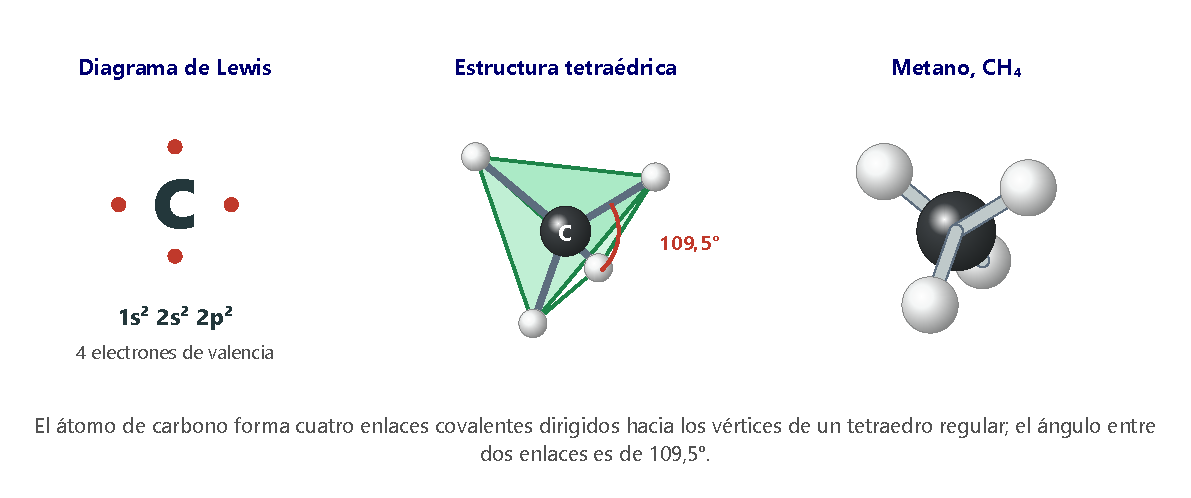
\includegraphics[width=0.85\textwidth]{images/UD7/tetraedro}
    \caption{El carbono forma cuatro enlaces dirigidos hacia los vértices de un tetraedro regular.}
    \label{fig:ud7-tetraedro}
\end{figure}

Según los enlaces que forme, el carbono presenta tres geometrías (figura~\ref{fig:ud7-enlaces}):

\begin{table}[H]
    \centering
    \caption{Tipos de carbono según sus enlaces}
    \vspace{-5pt}
    \begin{tabular}{@{}L{3.8cm}cccl@{}}
        \toprule
        \textbf{Enlaces del carbono} & \textbf{Hibridación} & \textbf{Geometría} & \textbf{Ángulo} & \textbf{Ejemplo} \\
        \midrule
        Cuatro sencillos & \(sp^3\) & tetraédrica & \ang{109.5} & etano, \ch{CH3-CH3} \\[3pt]
        Uno doble y dos sencillos & \(sp^2\) & plana triangular & \ang{120} & eteno, \ch{CH2=CH2} \\[3pt]
        Uno triple y uno sencillo, o dos dobles & \(sp\) & lineal & \ang{180} & etino, \ch{CH+CH} \\
        \bottomrule
    \end{tabular}
    \label{tab:ud7-hibridacion}
\end{table}

\begin{figure}[H]
    \centering
    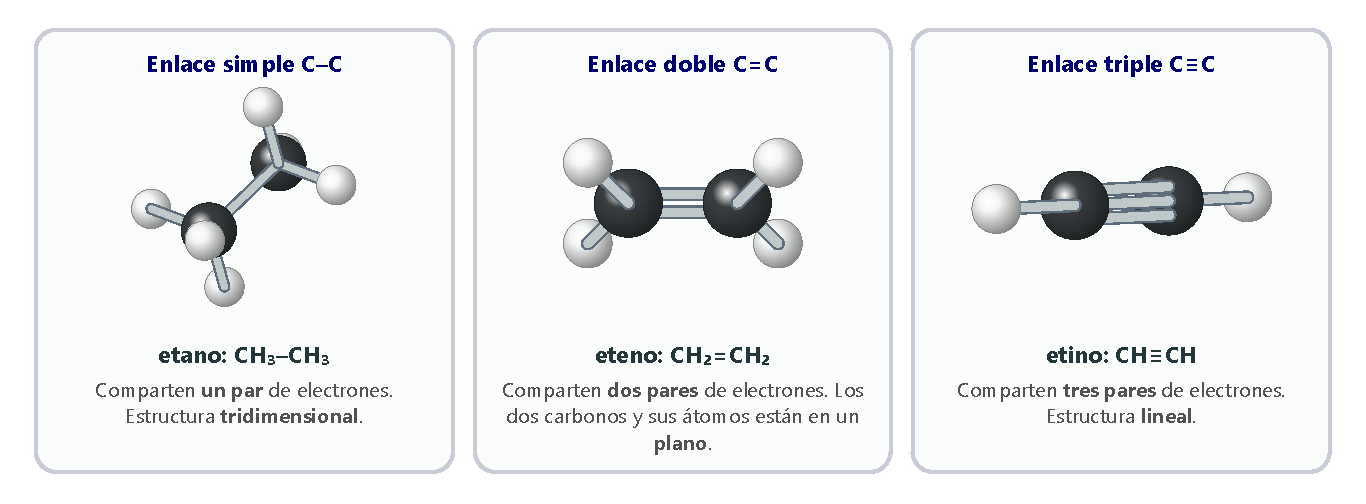
\includegraphics[width=0.85\textwidth]{images/UD7/enlaces_cc}
    \caption{Enlaces sencillo, doble y triple entre átomos de carbono.}
    \label{fig:ud7-enlaces}
\end{figure}

\subsection{Cadenas, enlaces y heteroátomos}

El enlace covalente \ch{C-C} es muy fuerte, y por eso los átomos de carbono pueden unirse entre sí formando \textbf{cadenas}
\textbf{abiertas} (lineales o ramificadas) o \textbf{cerradas} (anillos), a veces de miles de átomos:
\[ \underset{\text{lineal}}{\chemfig{C-C-C-C}} \qquad\quad
   \underset{\text{ramificada}}{\chemfig{C-C(-[6]C)-C-C}} \qquad\quad
   \underset{\text{cerrada}}{\chemfig{C*5(-C-C-C-C-)}} \]
Los compuestos que solo tienen enlaces sencillos entre carbonos son \textbf{saturados}; los que tienen algún enlace doble o triple
(enlaces múltiples o \textbf{insaturaciones}) son \textbf{insaturados}.

Además de hidrógeno, los compuestos del carbono pueden contener oxígeno, nitrógeno y, en menor cantidad, halógenos, azufre, fósforo e
incluso metales. Cualquier átomo distinto del C y el H en un compuesto orgánico es un \textbf{heteroátomo}.

\paragraph{Tipos de carbono.} Un carbono es \textbf{primario} si está unido a un solo carbono, \textbf{secundario} si está unido a
dos, \textbf{terciario} si está unido a tres y \textbf{cuaternario} si está unido a cuatro, sean los enlaces sencillos o múltiples.
En el 2,2,4-trimetilpentano, por ejemplo,
\[ \chemfig{\underset{1^\circ}{CH_3}-\underset{4^\circ}{C}(-[2]CH_3)(-[6]CH_3)-\underset{2^\circ}{CH_2}-\underset{3^\circ}{CH}(-[6]CH_3)-CH_3} \]

\begin{exercise}
    Indica la hibridación de cada carbono y los ángulos de enlace aproximados en el compuesto \ch{CH2=CH-CH2-C+CH}.
    \begin{solu}
        Numerando de izquierda a derecha: \textcolor{red}{C1 y C2, \(sp^2\) (\ang{120}); C3, \(sp^3\) (\ang{109.5}); C4 y C5,
        \(sp\) (\ang{180})}.
    \end{solu}
\end{exercise}

\begin{exercise}
    Clasifica los carbonos del compuesto \chemfig{CH_3-C(-[2]CH_3)(-[6]CH_3)-CH_2-CH(-[6]CH_3)-CH_3} en primarios, secundarios,
    terciarios y cuaternarios.
    \begin{solu}
        \textcolor{red}{5 primarios} (los cinco \ch{CH3}), \textcolor{red}{1 secundario} (el \ch{CH2}), \textcolor{red}{1
        terciario} (el \ch{CH}) y \textcolor{red}{1 cuaternario} (el C unido a cuatro carbonos). En total, 8 carbonos: es el
        2,2,4-trimetilpentano, \ch{C8H18}, el «isooctano» que se usa como referencia del octanaje de las gasolinas.
    \end{solu}
\end{exercise}

\begin{exercise}
    ¿Verdadero o falso? Justifica. a) Todos los compuestos con carbono son orgánicos. b) Wöhler demostró que las sustancias
    orgánicas pueden obtenerse a partir de sustancias inorgánicas. c) En el etino los átomos están en línea recta. d) Un compuesto
    con un enlace triple es saturado.
    \begin{solu}
        a) \textcolor{red}{Falso}: el \ch{CO}, el \ch{CO2} o los carbonatos son inorgánicos. b) \textcolor{red}{Verdadero}: sintetizó
        urea a partir de cianato de amonio. c) \textcolor{red}{Verdadero}: los carbonos son \(sp\) y los ángulos son de
        \ang{180}. d) \textcolor{red}{Falso}: es insaturado.
    \end{solu}
\end{exercise}

%========================================================================================
\section{Las fórmulas de los compuestos del carbono}\label{sec:ud7-formulas}
%========================================================================================

Las propiedades de una sustancia orgánica dependen no solo de los átomos que la forman, sino de \textbf{cómo están unidos}. Por eso,
además de las fórmulas empírica y molecular que ya conoces, necesitamos fórmulas que muestren los enlaces.

\subsection{Fórmulas empírica y molecular}

\begin{definition}[Fórmula empírica y fórmula molecular]
    La \textbf{fórmula empírica} indica la \textbf{proporción} más sencilla en que están los átomos de cada elemento. La
    \textbf{fórmula molecular} indica el \textbf{número real} de átomos de cada elemento en una molécula; es un múltiplo entero de
    la empírica y se obtiene con ella y la \textbf{masa molar}.
\end{definition}

El acetileno (\ch{C2H2}) y el benceno (\ch{C6H6}) tienen la misma fórmula empírica, \ch{CH}, pero distinta fórmula molecular. La
fórmula empírica de un compuesto orgánico se determina en el laboratorio quemando una masa conocida y midiendo el \ch{CO2} y el
\ch{H2O} que se forman: \textbf{todo el C pasa al \ch{CO2} y todo el H al \ch{H2O}}. La masa molar se obtiene con la densidad del
gas, la ecuación de los gases o las propiedades coligativas (unidades 1 y 2).

\begin{example}
    \textbf{Fórmula de un hidrocarburo por combustión.} Al quemar por completo un hidrocarburo se obtienen \qty{26.4}{\gram} de
    \ch{CO2} y \qty{13.5}{\gram} de \ch{H2O}. Su masa molar es \qty{58}{\gram\per\mol}. Halla sus fórmulas empírica y molecular.

    \textbf{Solución.} \(\ch{C_xH_y + O2 -> CO2 + H2O}\); \(M(\ch{CO2}) = \qty{44}{\gram\per\mol}\), \(M(\ch{H2O}) =
    \qty{18}{\gram\per\mol}\).
    \[ n(\ch{C}) = \frac{26{,}4}{44} = \qty{0.600}{\mol} \qquad n(\ch{H}) = 2 \cdot \frac{13{,}5}{18} = \qty{1.50}{\mol} \]
    Dividimos por el menor: \(\dfrac{0{,}600}{0{,}600} = 1\); \(\dfrac{1{,}50}{0{,}600} = 2{,}5\). Multiplicando por 2 para tener
    enteros: \(\ch{C2H5}\), con masa \(2 \cdot 12 + 5 = 29\). Como \(58/29 = 2\), la fórmula molecular es \(\ch{(C2H5)2} =
    \ch{C4H10}\) (butano o metilpropano).
\end{example}

\begin{example}
    \textbf{Compuesto con oxígeno.} Una muestra de \qty{2.30}{\gram} de un compuesto de C, H y O produce al arder \qty{4.40}{\gram}
    de \ch{CO2} y \qty{2.70}{\gram} de \ch{H2O}. Una masa de \qty{0.46}{\gram} de su vapor ocupa \qty{306}{\mL} a
    \qty{100}{\degreeCelsius} y \qty{1}{\atm}. Halla su fórmula molecular.

    \textbf{Solución.} \(m(\ch{C}) = 4{,}40 \cdot \frac{12}{44} = \qty{1.20}{\gram}\) (\(\qty{0.100}{\mol}\));
    \(m(\ch{H}) = 2{,}70 \cdot \frac{2}{18} = \qty{0.300}{\gram}\) (\(\qty{0.300}{\mol}\)). El oxígeno es lo que falta:
    \(m(\ch{O}) = 2{,}30 - 1{,}20 - 0{,}300 = \qty{0.80}{\gram}\) (\(\qty{0.050}{\mol}\)). Proporción
    \(0{,}100 : 0{,}300 : 0{,}050 = 2 : 6 : 1\): fórmula empírica \ch{C2H6O} (\(M = 46\)). Con los gases:
    \[ M = \frac{m\,R\,T}{p\,V} = \frac{0{,}46 \cdot 0{,}082 \cdot 373}{1 \cdot 0{,}306} = \qty{46}{\gram\per\mol} \]
    La fórmula molecular es \ch{C2H6O}: puede ser el etanol, \ch{CH3-CH2OH}, o el dimetil éter, \ch{CH3-O-CH3}. Para saber cuál
    es hace falta otro dato, como su punto de ebullición.
\end{example}

\begin{remark}
    La estructura exacta de un compuesto se determina con técnicas como la espectroscopía infrarroja, la resonancia magnética
    nuclear (RMN), la espectrometría de masas o la difracción de rayos X.
\end{remark}

\subsection{Fórmulas estructurales}

\begin{table}[H]
    \centering
    \caption{Tipos de fórmulas estructurales, con el ejemplo del butano}
    \vspace{-5pt}
    \begin{tabular}{@{}L{2.65cm}L{6cm}C{5.35cm}@{}}
        \toprule
        \textbf{Fórmula} & \textbf{Qué representa} & \textbf{Butano} \\
        \midrule
        Desarrollada & Todos los átomos y todos los enlaces, en el plano. No informa de la disposición en el espacio. &
        \chemfig{H-C(-[2]H)(-[6]H)-C(-[2]H)(-[6]H)-C(-[2]H)(-[6]H)-C(-[2]H)(-[6]H)-H} \\[3pt]
        Semidesarrollada & Solo los enlaces entre carbonos (y con los grupos funcionales); los H se agrupan con su carbono. &
        \ch{CH3-CH2-CH2-CH3} o \ch{CH3-(CH2)2-CH3} \\[3pt]
        En esqueleto (zigzag) & Cada vértice y cada extremo es un carbono; los H unidos a C no se escriben. &
        \chemfig{-[:30]-[:-30]-[:30]} \\[3pt]
        Geométrica o tridimensional & La disposición en el espacio: las cuñas gruesas salen del papel y las discontinuas se
        alejan. & \chemfig{H_3C-C(<[2]H)(<:[6]H)-C(<[2]H)(<:[6]H)-CH_3} \\
        \bottomrule
    \end{tabular}
    \label{tab:ud7-formulas}
\end{table}

Los \textbf{modelos moleculares} de bolas y varillas o de esferas permiten ver la forma de la molécula, los ángulos de enlace y el
tamaño relativo de los átomos.

\begin{exercise}
    Al quemar un hidrocarburo gaseoso se obtienen \qty{13.2}{\gram} de \ch{CO2} y \qty{5.4}{\gram} de \ch{H2O}. Si su densidad en
    condiciones normales es \qty{1.875}{\gram\per\litre}, halla: a) su fórmula empírica; b) su fórmula molecular.
    \begin{solu}
        \textcolor{blue}{\(n(\ch{C}) = 13{,}2/44 = \qty{0.30}{\mol}\); \(n(\ch{H}) = 2 \cdot 5{,}4/18 = \qty{0.60}{\mol}\); proporción
        1 : 2.} a) \textcolor{red}{\ch{CH2}}. b) \textcolor{blue}{\(M = 1{,}875 \cdot 22{,}4 = \qty{42}{\gram\per\mol}\); \(42/14 = 3\).}
        \textcolor{red}{\ch{C3H6}}.
    \end{solu}
\end{exercise}

\begin{exercise}
    Al quemar \qty{1.80}{\gram} de un azúcar formado por C, H y O se obtienen \qty{2.64}{\gram} de \ch{CO2} y \qty{1.08}{\gram} de
    \ch{H2O}. Su masa molar es \qty{180}{\gram\per\mol}. Halla sus fórmulas empírica y molecular.
    \begin{solu}
        \textcolor{blue}{\(m(\ch{C}) = 2{,}64 \cdot 12/44 = \qty{0.72}{\gram}\) (\qty{0.060}{\mol}); \(m(\ch{H}) = 1{,}08 \cdot 2/18 =
        \qty{0.12}{\gram}\) (\qty{0.12}{\mol}); \(m(\ch{O}) = 1{,}80 - 0{,}72 - 0{,}12 = \qty{0.96}{\gram}\) (\qty{0.060}{\mol}).
        Proporción 1 : 2 : 1.} Empírica \textcolor{red}{\ch{CH2O}} (\(M = 30\)); \(180/30 = 6\): molecular
        \textcolor{red}{\ch{C6H12O6}} (glucosa o fructosa).
    \end{solu}
\end{exercise}

\begin{exercise}
    Un hidrocarburo contiene un 85,7\,\% de carbono. Una muestra de \qty{0.70}{\gram} de su vapor ocupa \qty{224}{\mL} en
    condiciones normales. Halla su fórmula molecular.
    \begin{solu}
        \textcolor{blue}{En \qty{100}{\gram}: \(85{,}7/12 = \qty{7.14}{\mol}\) de C y \(14{,}3/1 = \qty{14.3}{\mol}\) de H: proporción
        1 : 2, \ch{CH2}. \(n = 0{,}224/22{,}4 = \qty{0.0100}{\mol}\); \(M = 0{,}70/0{,}0100 = \qty{70}{\gram\per\mol}\); \(70/14 = 5\).}
        \textcolor{red}{\ch{C5H10}}.
    \end{solu}
\end{exercise}

\begin{exercise}
    Escribe la fórmula semidesarrollada y la molecular de los compuestos representados en esqueleto: a) \chemfig{-[:30]-[:-30]-[:30]-[:-30]};
    b) \chemfig{-[:30]=[:-30]-[:30]}; c) \chemfig{-[:30]-[:-30](-[6])-[:30]}.
    \begin{solu}
        a) \textcolor{red}{\ch{CH3-CH2-CH2-CH2-CH3}, \ch{C5H12}} (pentano). b) \textcolor{red}{\ch{CH3-CH=CH-CH3}, \ch{C4H8}}
        (but-2-eno). c) \textcolor{red}{\chemfig{CH_3-CH_2-CH(-[6]CH_3)-CH_3}, \ch{C5H12}} (2-metilbutano).
    \end{solu}
\end{exercise}

%========================================================================================
\section{Los compuestos del carbono: generalidades}\label{sec:ud7-generalidades}
%========================================================================================

\subsection{Estructura de los compuestos orgánicos}

\begin{definition}[Grupo funcional, familia y serie homóloga]
    Un \textbf{grupo funcional} es un átomo o grupo de átomos responsable del comportamiento químico de la sustancia: le da sus
    \textbf{propiedades características}. Los compuestos con el mismo grupo funcional forman una \textbf{familia} (por ejemplo, los
    alcoholes, con el grupo \ch{-OH}). Dentro de una familia, los compuestos que solo se diferencian en el número de grupos
    \ch{-CH2-} forman una \textbf{serie homóloga}.
\end{definition}

El etanol (\ch{CH3-CH2OH}), el butan-1-ol (\ch{CH3-CH2-CH2-CH2OH}) y el fenol (\ch{C6H5OH}) son de la misma familia, porque tienen
el grupo \ch{-OH}; además, el etanol y el butan-1-ol pertenecen a la misma serie homóloga.

\begin{itemize}
    \item La \textbf{cadena principal} es la cadena de átomos de carbono que se toma como base para el nombre. Si hay grupos
    funcionales, debe contener el \textbf{grupo funcional principal}.
    \item Los \textbf{sustituyentes} son las cadenas laterales (\textbf{ramificaciones}) y los grupos funcionales que no son el
    principal.
    \item Un \textbf{radical} (R) es un grupo de átomos que tiene un electrón desapareado, normalmente porque ha perdido un hidrógeno.
    Los radicales libres son inestables y muy reactivos; como sustituyentes, se unen a la cadena principal por ese electrón.
\end{itemize}

\subsection{Clasificación de los compuestos orgánicos}

\begin{table}[H]
    \centering
    \caption{Clasificación de los compuestos orgánicos que estudiaremos}
    \vspace{-5pt}
    \begin{tabular}{@{}L{5cm}L{4.5cm}L{4.5cm}@{}}
        \toprule
        \textbf{Hidrocarburos} (solo C y H) & \textbf{Compuestos oxigenados} & \textbf{Compuestos nitrogenados} \\
        \midrule
        Alifáticos de cadena abierta: alcanos, alquenos y alquinos & Alcoholes y fenoles & Aminas \\[3pt]
        Alifáticos de cadena cerrada: cicloalcanos, cicloalquenos y cicloalquinos & Éteres & Amidas \\[3pt]
        Aromáticos: benceno y derivados & Aldehídos y cetonas & Nitrilos \\[3pt]
        (Derivados halogenados) & Ácidos carboxílicos, ésteres y sales & \\
        \bottomrule
    \end{tabular}
    \label{tab:ud7-clasificacion}
\end{table}

Los hidrocarburos son el «esqueleto» del resto de los compuestos, y por eso empezaremos por ellos.

\begin{remark}
    Los primeros compuestos orgánicos recibieron nombres según su origen: el ácido \textbf{fórmico} se obtuvo de las hormigas
    (\emph{formica}, en latín), el ácido \textbf{láctico} de la leche y la \textbf{cadaverina}, de la descomposición de los
    cadáveres. Con millones de compuestos hace falta una nomenclatura \textbf{sistemática}, cuyas normas fija la \textbf{IUPAC}
    (Unión Internacional de Química Pura y Aplicada). Algunos nombres tradicionales, como acetona, ácido acético o benceno, siguen
    aceptados.
\end{remark}

\subsection{Prefijos que indican el número de carbonos}

\begin{table}[H]
    \centering
    \caption{Prefijos para el número de carbonos de una cadena}
    \vspace{-5pt}
    \begin{tabular}{@{}clclcl@{}}
        \toprule
        \textbf{N.º de C} & \textbf{Prefijo} & \textbf{N.º de C} & \textbf{Prefijo} & \textbf{N.º de C} & \textbf{Prefijo} \\
        \midrule
        1 & met- & 6 & hex- & 11 & undec- \\[3pt]
        2 & et- & 7 & hept- & 12 & dodec- \\[3pt]
        3 & prop- & 8 & oct- & 13 & tridec- \\[3pt]
        4 & but- & 9 & non- & 14 & tetradec- \\[3pt]
        5 & pent- & 10 & dec- & 20 & icos- \\
        \bottomrule
    \end{tabular}
    \label{tab:ud7-prefijos}
\end{table}

\paragraph{Reglas generales de la nomenclatura.}
\begin{itemize}
    \item Los enlaces múltiples se indican con las terminaciones \textbf{-en-} (doble) e \textbf{-in-} (triple).
    \item El grupo funcional principal se indica con un \textbf{sufijo}; los demás grupos funcionales, con un \textbf{prefijo}.
    \item La posición de los sustituyentes, los enlaces múltiples y el grupo principal se indica con números o
    \textbf{localizadores}, que se colocan \textbf{delante} de lo que señalan, separados por un \textbf{guion}: but-1-eno,
    2-metilpropano. Los números se separan entre sí con comas: 2,3-dimetilbutano.
    \item Si hay varios sustituyentes iguales se usan los prefijos \textbf{di-}, \textbf{tri-}, \textbf{tetra-}\ldots Los
    sustituyentes distintos se nombran por \textbf{orden alfabético}, sin tener en cuenta esos prefijos multiplicadores.
\end{itemize}

\subsection{Prioridad de los grupos funcionales}

Si un compuesto tiene varios grupos funcionales, el principal (el que se nombra como sufijo) es el de mayor prioridad según este
orden:

\begin{table}[H]
    \centering
    \caption{Grupos funcionales por orden de prioridad decreciente}
    \vspace{-5pt}
    \begin{tabular}{@{}clcll@{}}
        \toprule
        \textbf{Orden} & \textbf{Función} & \textbf{Grupo} & \makecell{\textbf{Sufijo}\\\textbf{(principal)}} & \makecell{\textbf{Prefijo}\\\textbf{(sustituyente)}} \\
        \midrule
        1 & Ácido carboxílico & \ch{-COOH} & ácido \ldots-oico & carboxi- \\[3pt]
        2 & Éster & \ch{-COO-R} & \ldots-oato de \ldots-ilo & (alcoxicarbonil-) \\[3pt]
        3 & Amida & \ch{-CONH2} & -amida & carbamoil- \\[3pt]
        4 & Nitrilo & \ch{-C+N} & -nitrilo & ciano- \\[3pt]
        5 & Aldehído & \ch{-CHO} & -al & formil- u oxo- \\[3pt]
        6 & Cetona & \ch{-CO-} & -ona & oxo- \\[3pt]
        7 & Alcohol & \ch{-OH} & -ol & hidroxi- \\[3pt]
        8 & Amina & \ch{-NH2} & -amina & amino- \\[3pt]
        9 & Éter & \ch{-O-} & (\ldots éter) & alcoxi- (metoxi-\ldots) \\
        \midrule
        — & Halógeno & \ch{-X} & — & fluoro-, cloro-, bromo-, yodo- \\[3pt]
        — & Radical alquilo & \ch{-R} & — & metil-, etil-\ldots \\
        \bottomrule
    \end{tabular}
    \label{tab:ud7-prioridad}
\end{table}

En los grupos \ch{-COOH}, \ch{-CONH2}, \ch{-C+N} y \ch{-CHO} el carbono del grupo forma parte de la cadena principal y se cuenta
en el nombre: \ch{CH3-COOH} es el ácido \emph{etanoico}, con dos carbonos. Los halógenos y los radicales alquilo nunca son grupo
principal: siempre se nombran como prefijos.

\begin{definition}[Cómo nombrar un compuesto orgánico]
    \leavevmode % el título de la definición en su propia línea, la lista debajo
    \begin{enumerate}
        \item Identifica el \textbf{grupo funcional principal}, que se nombrará con su \textbf{sufijo}.
        \item Elige la \textbf{cadena principal}: la que contiene el grupo principal y, entre ellas, la más larga.
        \item \textbf{Numera} la cadena dando al grupo principal el localizador más bajo posible; después, a los enlaces múltiples y,
        por último, a los sustituyentes.
        \item Nombra los \textbf{sustituyentes} con sus prefijos y localizadores, por orden alfabético.
        \item Nombra la cadena principal con el prefijo del número de carbonos, los enlaces múltiples (-an-, -en-, -in-) y el sufijo del
        grupo principal.
    \end{enumerate}
    Para \textbf{formular}: dibuja la cadena principal, numérala, coloca los enlaces múltiples, los grupos funcionales y los
    sustituyentes y, al final, completa con hidrógenos hasta que cada carbono tenga cuatro enlaces.
\end{definition}

\begin{example}
    \textbf{Analizar un nombre.} Explica qué indica cada parte del nombre \emph{ácido 3-hidroxi-6-metilhept-4-enoico} y formula
    el compuesto.

    \textbf{Solución.}
    \begin{itemize}
        \item \emph{ácido \ldots-oico}: el grupo principal es \ch{-COOH}; su carbono es el C1.
        \item \emph{hept-}: la cadena principal tiene 7 carbonos.
        \item \emph{-4-en-}: hay un doble enlace entre los carbonos 4 y 5.
        \item \emph{3-hidroxi}: un grupo \ch{-OH} en el C3; \emph{6-metil}: un radical \ch{-CH3} en el C6 (los sustituyentes van
        en orden alfabético: h antes que m).
    \end{itemize}
    \[ \chemfig{CH_3-CH(-[6]CH_3)-CH=CH-CH(-[6]OH)-CH_2-COOH} \]
\end{example}

\begin{exercise}
    Indica el grupo funcional y la familia de cada compuesto: a) \ch{CH3-CH2-CHO}; b) \ch{CH3-CO-CH3}; c) \ch{CH3-CH2-COOH};
    d) \ch{CH3-NH-CH3}; e) \ch{CH3-COO-CH3}; f) \ch{CH3-O-CH2-CH3}; g) \ch{CH3-CHOH-CH3}; h) \ch{CH3-CO-NH2}.
    \begin{solu}
        a) \textcolor{red}{\ch{-CHO}, aldehído}; b) \textcolor{red}{\ch{-CO-}, cetona}; c) \textcolor{red}{\ch{-COOH}, ácido
        carboxílico}; d) \textcolor{red}{\ch{-NH-}, amina} (secundaria); e) \textcolor{red}{\ch{-COO-}, éster}; f)
        \textcolor{red}{\ch{-O-}, éter}; g) \textcolor{red}{\ch{-OH}, alcohol}; h) \textcolor{red}{\ch{-CONH2}, amida}.
    \end{solu}
\end{exercise}

\begin{exercise}
    ¿Cuáles de estos compuestos pertenecen a la misma serie homóloga? \ch{CH3OH}, \ch{CH3-CH2-CH2OH}, \ch{CH3-O-CH3},
    \ch{CH3-CH2-CH2-CH2OH}, \ch{CH3-CHO}, \ch{CH3-CH2OH}.
    \begin{solu}
        \textcolor{red}{\ch{CH3OH}, \ch{CH3-CH2OH}, \ch{CH3-CH2-CH2OH} y \ch{CH3-CH2-CH2-CH2OH}}: son alcoholes con el \ch{-OH} en un
        extremo y solo se diferencian en grupos \ch{-CH2-}. El \ch{CH3-O-CH3} es un éter y el \ch{CH3-CHO}, un aldehído.
    \end{solu}
\end{exercise}

\begin{exercise}
    Indica el grupo principal, el número de carbonos de la cadena principal, los enlaces múltiples y los sustituyentes de:
    a) hepta-1,6-diin-4-ol; b) ácido 3-hidroxibutanoico; c) 2,3-dimetilpent-4-enal; d) 4-etil-6-metilhept-3-en-2-ona.
    \begin{solu}
        a) \textcolor{red}{\ch{-OH} en C4; 7 C; triples entre C1-C2 y C6-C7; sin sustituyentes}. b) \textcolor{red}{\ch{-COOH} (C1);
        4 C; sin enlaces múltiples; \ch{-OH} en C3}. c) \textcolor{red}{\ch{-CHO} (C1); 5 C; doble entre C4 y C5; metilos en C2 y
        C3}. d) \textcolor{red}{\ch{-CO-} en C2; 7 C; doble entre C3 y C4; etilo en C4 y metilo en C6}.
    \end{solu}
\end{exercise}

%========================================================================================
\section{Hidrocarburos}\label{sec:ud7-hidrocarburos}
%========================================================================================

Los \textbf{hidrocarburos} son compuestos formados solo por carbono e hidrógeno. Se clasifican según su cadena y sus enlaces
(figura~\ref{fig:ud7-clasificacion}).

\begin{figure}[H]
    \centering
    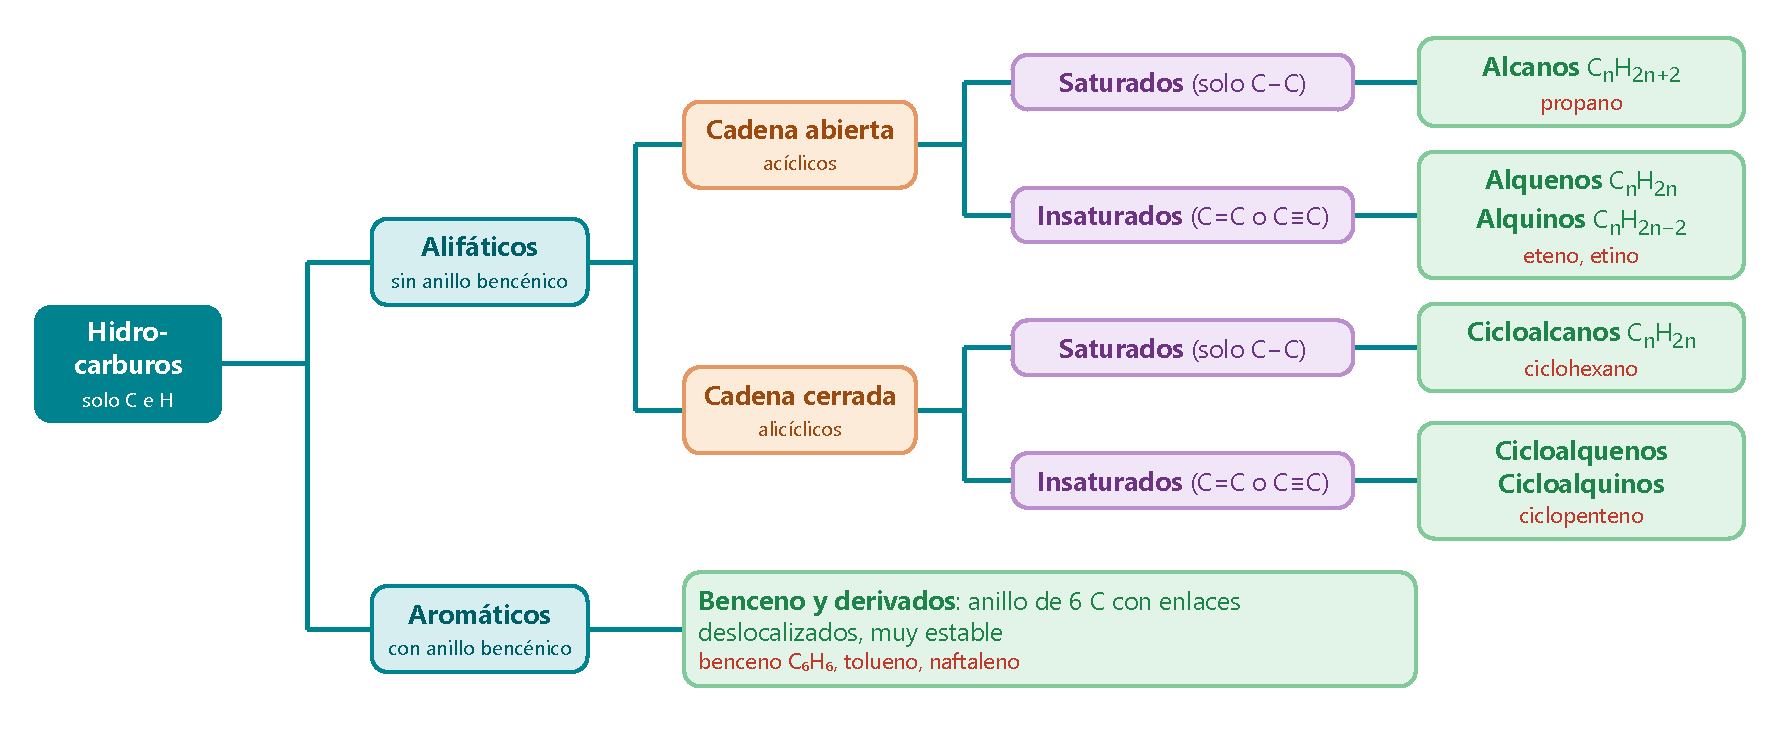
\includegraphics[width=\textwidth]{images/UD7/clasificacion_hidrocarburos}
    \caption{Clasificación de los hidrocarburos.}
    \label{fig:ud7-clasificacion}
\end{figure}

\subsection{Alcanos}

Los \textbf{alcanos} son hidrocarburos de cadena abierta con todos los enlaces \ch{C-C} sencillos. Su fórmula general es
\(\ch{C_nH_{2n+2}}\).

\paragraph{Alcanos de cadena lineal.} Se nombran con el prefijo del número de carbonos y la terminación \textbf{-ano}: \ch{CH4},
metano; \ch{CH3-CH2-CH2-CH3}, butano; \ch{CH3-(CH2)5-CH3}, heptano.

\paragraph{Radicales alquilo.} Son alcanos que han perdido un hidrógeno de un extremo. Se nombran cambiando -ano por \textbf{-ilo}
(o \textbf{-il} cuando se nombran como sustituyentes): \ch{CH3-}, metilo; \ch{CH3-CH2-}, etilo; \ch{CH3-CH2-CH2-}, propilo;
\ch{CH3-(CH2)3-}, butilo.

\paragraph{Alcanos ramificados.} Las ramificaciones son radicales alquilo unidos a la cadena principal. Para nombrarlos:
\begin{enumerate}
    \item Elige como cadena principal la \textbf{más larga}. Si hay varias igual de largas, la que tenga \textbf{más
    ramificaciones}.
    \item \textbf{Numera} la cadena desde el extremo que dé los \textbf{localizadores más bajos} a las ramificaciones (en el primer
    punto de diferencia). Si sigue habiendo empate, se da el localizador más bajo a la ramificación que se cita antes por orden
    alfabético.
    \item Nombra los radicales por \textbf{orden alfabético} con su localizador delante. Si hay varios iguales, se agrupan con
    di-, tri-\ldots\ y se escriben todos los localizadores, aunque se repitan: 3,3-dietil.
    \item Termina con el nombre de la cadena principal.
\end{enumerate}

\begin{example}
    \textbf{Nombrar un alcano ramificado.} Nombra el compuesto
    \[ \chemfig{CH_3-CH(-[6]CH_3)-CH(-[6]CH_2-[0]CH_3)-CH_2-CH_2-CH_3} \]

    \textbf{Solución.} Hay dos cadenas de 6 carbonos: la horizontal y la que entra por el etilo. La horizontal tiene dos
    ramificaciones (metilo y etilo); la otra, solo una (un radical de tres carbonos). Elegimos la horizontal. Numerando desde la
    izquierda, los localizadores son \{2, 3\}; desde la derecha, \{4, 5\}: numeramos desde la izquierda. Por orden alfabético
    (e antes que m): \textbf{3-etil-2-metilhexano}.
\end{example}

\begin{example}
    \textbf{Formular un alcano ramificado.} Formula el 5-etil-2,3,3-trimetilheptano.

    \textbf{Solución.} Cadena de 7 carbonos; metilos en C2 y dos en C3; etilo en C5. Completamos con hidrógenos:
    \[ \chemfig{CH_3-CH(-[6]CH_3)-C(-[2]CH_3)(-[6]CH_3)-CH_2-CH(-[6]CH_2-[0]CH_3)-CH_2-CH_3} \]
    La fórmula molecular es \ch{C12H26}, que cumple \(\ch{C_nH_{2n+2}}\).
\end{example}

\paragraph{Radicales complejos.} Los radicales ramificados se nombran como si fueran compuestos, numerando desde el carbono unido
a la cadena principal, y su nombre se escribe entre paréntesis: \ch{CH3-CH(CH3)-CH2-}, (2-metilpropil). La IUPAC admite nombres
tradicionales para los más sencillos:

\begin{table}[H]
    \centering
    \caption{Radicales ramificados con nombre tradicional}
    \vspace{-5pt}
    \begin{tabular}{@{}lll@{}}
        \toprule
        \textbf{Radical} & \textbf{Nombre tradicional} & \textbf{Nombre sistemático} \\
        \midrule
        \chemfig{CH_3-CH(-[6]CH_3)-} & isopropil & (1-metiletil) \\[3pt]
        \chemfig{CH_3-CH(-[6]CH_3)-CH_2-} & isobutil & (2-metilpropil) \\[3pt]
        \chemfig{CH_3-CH_2-CH(-[6]CH_3)-} & \emph{sec}-butil & (1-metilpropil) \\[3pt]
        \chemfig{CH_3-C(-[2]CH_3)(-[6]CH_3)-} & \emph{terc}-butil & (1,1-dimetiletil) \\[3pt]
        \chemfig{CH_3-C(-[2]CH_3)(-[6]CH_3)-CH_2-} & neopentil & (2,2-dimetilpropil) \\
        \bottomrule
    \end{tabular}
    \label{tab:ud7-radicales}
\end{table}

Al ordenar alfabéticamente, iso- y neo- sí cuentan (isopropil va por la i), pero \emph{sec}- y \emph{terc}- no (\emph{terc}-butil va
por la b).

\paragraph{Propiedades y aplicaciones.}
\begin{itemize}
    \item Son \textbf{apolares}: sus moléculas se atraen solo por fuerzas de dispersión, por lo que sus puntos de fusión y
    ebullición son \textbf{bajos} y aumentan con el número de carbonos (figura~\ref{fig:ud7-ebullicion}). A temperatura ambiente
    son gases hasta 4 carbonos, líquidos hasta unos 17 y sólidos a partir de ahí (parafinas). Las ramificaciones hacen la molécula
    más compacta y \textbf{bajan} el punto de ebullición.
    \item Son \textbf{insolubles en agua} y solubles en disolventes apolares; su densidad es menor que la del agua.
    \item Son \textbf{poco reactivos} (de ahí el nombre de \emph{parafinas}, «poca afinidad»). Sus reacciones más importantes son la
    \textbf{combustión} y el \textbf{craqueo}, en el que los alcanos grandes se rompen con calor en otros más pequeños.
    \item Se obtienen del \textbf{petróleo} y del \textbf{gas natural} y se usan sobre todo como \textbf{combustibles}.
\end{itemize}

\begin{figure}[H]
    \centering
    \begin{tikzpicture}
        \begin{axis}[grafica, width=0.62\linewidth, height=5.5cm,
            xlabel={Número de carbonos}, ylabel={\(T_\text{eb}\) (\unit{\degreeCelsius})},
            xmin=0, xmax=11, ymin=-200, ymax=200, xtick={1,...,10}, ytick={-200,-100,...,200}]
            \addplot[thick, mark=*, color=ocre] coordinates {(1,-162) (2,-89) (3,-42) (4,-0.5) (5,36) (6,69) (7,98) (8,126) (9,151) (10,174)};
            \addplot[dashed, gray] coordinates {(0,25) (11,25)};
            \node[font=\scriptsize, gray, anchor=south west] at (axis cs:0.2,25) {\qty{25}{\degreeCelsius}};
        \end{axis}
    \end{tikzpicture}
    \caption{Temperatura de ebullición de los alcanos lineales: por debajo de la línea de \qty{25}{\degreeCelsius}, gases.}
    \label{fig:ud7-ebullicion}
\end{figure}

\begin{exercise}
    Formula: a) hexano; b) 2,3-dimetilpentano; c) 4-etil-3,3-dimetilheptano; d) 5-isopropil-3-metilnonano; e)
    4-\emph{terc}-butiloctano.
    \begin{solu}
        a) \textcolor{red}{\ch{CH3-(CH2)4-CH3}}. b) \textcolor{red}{\chemfig{CH_3-CH(-[6]CH_3)-CH(-[6]CH_3)-CH_2-CH_3}}.
        c) \textcolor{red}{\chemfig{CH_3-CH_2-C(-[2]CH_3)(-[6]CH_3)-CH(-[6]CH_2-[0]CH_3)-CH_2-CH_2-CH_3}}.
        d) \textcolor{red}{\chemfig{CH_3-CH_2-CH(-[6]CH_3)-CH_2-CH(-[6]CH(-[0]CH_3)-[6]CH_3)-(CH_2)_3-CH_3}}.
        e) \textcolor{red}{\chemfig{CH_3-CH_2-CH_2-CH(-[6]C(-[0]CH_3)(-[4]H_3C)-[6]CH_3)-(CH_2)_3-CH_3}}.
    \end{solu}
\end{exercise}

\begin{exercise}
    Nombra: a) \ch{CH3-(CH2)6-CH3};
    \begin{gather*}
        \text{b)}\ \chemfig{CH_3-C(-[2]CH_3)(-[6]CH_3)-CH(-[6]CH_3)-CH_3} \qquad
        \text{c)}\ \chemfig{CH_3-CH(-[6]CH_3)-CH_2-CH(-[6]CH_2-[0]CH_3)-CH_2-CH_3} \\
        \text{d)}\ \chemfig{CH_3-CH_2-CH(-[6]CH_3)-CH(-[6]CH_3)-CH_2-CH_2-CH_3} \qquad
        \text{e)}\ \chemfig{CH_3-CH(-[6]CH_3)-CH(-[2]CH_2-[0]CH_3)-CH(-[6]CH_3)-CH_3}
    \end{gather*}
    \begin{solu}
        a) \textcolor{red}{Octano}. b) \textcolor{red}{2,2,3-trimetilbutano}. c) \textcolor{blue}{Cadena de 6 C; localizadores
        \{2, 4\} frente a \{3, 5\}:} \textcolor{red}{4-etil-2-metilhexano}. d) \textcolor{red}{3,4-dimetilheptano}.
        e) \textcolor{blue}{Todas las cadenas posibles tienen 5 C; la horizontal tiene tres ramificaciones:}
        \textcolor{red}{3-etil-2,4-dimetilpentano}.
    \end{solu}
\end{exercise}

\begin{exercise}
    Ordena de menor a mayor punto de ebullición y justifica: hexano, propano, decano y 2,2-dimetilbutano.
    \begin{solu}
        \textcolor{red}{Propano \(<\) 2,2-dimetilbutano \(<\) hexano \(<\) decano}. Las fuerzas de dispersión crecen con el tamaño de
        la molécula. El hexano y el 2,2-dimetilbutano tienen la misma masa (\ch{C6H14}), pero la forma compacta del segundo reduce la
        superficie de contacto entre moléculas (hierven a 69 y \qty{50}{\degreeCelsius}).
    \end{solu}
\end{exercise}

\begin{exercise}
    a) Escribe y ajusta la combustión del octano, \ch{C8H18}. b) ¿Qué masa de \ch{CO2} se emite al quemar \qty{1}{\litre} de
    gasolina, suponiendo que es octano puro de densidad \qty{0.70}{\kilo\gram\per\litre}?
    \begin{solu}
        a) \textcolor{red}{\ch{2 C8H18 + 25 O2 -> 16 CO2 + 18 H2O}}. b) \textcolor{blue}{\(n(\ch{C8H18}) = 700/114 = \qty{6.14}{\mol}\);
        \(n(\ch{CO2}) = 8 \cdot 6{,}14 = \qty{49.1}{\mol}\).} \(m = 49{,}1 \cdot 44 = \textcolor{red}{\qty{2.16}{\kilo\gram}}\).
    \end{solu}
\end{exercise}

\subsection{Alquenos y alquinos}

Los \textbf{alquenos} tienen algún enlace doble \ch{C=C}, y los \textbf{alquinos}, algún enlace triple \ch{C+C}. Con una sola
insaturación, sus fórmulas generales son \(\ch{C_nH_{2n}}\) y \(\ch{C_nH_{2n-2}}\).

\paragraph{Cadena lineal con una insaturación.} Se cambia la terminación -ano por \textbf{-eno} (doble) o \textbf{-ino} (triple):
\ch{CH2=CH2}, eteno o etileno; \ch{CH+CH}, etino o acetileno. A partir de 4 carbonos hay que indicar la posición del enlace
múltiple: se numera desde el extremo \textbf{más próximo} a él y se escribe el \textbf{menor} de los dos localizadores delante de la
terminación: \ch{CH2=CH-CH2-CH3}, but-1-eno; \ch{CH3-C+C-CH2-CH3}, pent-2-ino.

\paragraph{Varias insaturaciones.} Se usan \textbf{-dieno}, \textbf{-trieno}, \textbf{-diino}\ldots, y se añade una «a» a la raíz
cuando lo pide la pronunciación: buta-1,3-dieno, hexa-1,3,5-trieno. Si hay dobles y triples enlaces, se nombran primero los
dobles (\textbf{-en-}) y luego los triples (\textbf{-ino}), y se numera para que el \textbf{conjunto} de los localizadores de los
enlaces múltiples sea el más bajo; si hay empate, los dobles enlaces reciben los más bajos:
\[ \underset{\text{pent-1-en-4-ino}}{\ch{CH2=CH-CH2-C+CH}} \qquad\qquad
   \underset{\text{hexa-1,3-dien-5-ino}}{\ch{CH+C-CH=CH-CH=CH2}} \]

\paragraph{Radicales.} Los radicales con un doble o triple enlace se numeran desde el carbono por el que se unen: \ch{CH2=CH-},
etenil (vinil); \ch{CH2=CH-CH2-}, prop-2-enil (alil); \ch{CH+C-}, etinil.

\paragraph{Alquenos y alquinos ramificados.} Las ramificaciones se nombran delante, en orden alfabético. Según las recomendaciones
actuales de la IUPAC, la cadena principal se elige así (si hay empate en un criterio, se pasa al siguiente):
\begin{enumerate}
    \item la de mayor número de carbonos;
    \item la de mayor número de enlaces múltiples;
    \item la de mayor número de enlaces dobles.
\end{enumerate}
Después, se numera para dar los localizadores más bajos a los enlaces múltiples en conjunto, luego a los dobles y, por último, a
las ramificaciones.

\begin{example}
    \textbf{Nombrar alquenos y alquinos.} Nombra:
    \begin{gather*}
        \text{a)}\ \chemfig{CH_3-CH=C(-[6]CH_3)-CH_2-CH_3} \qquad \text{b)}\ \chemfig{CH_2=CH-CH(-[6]CH_2-[0]CH_3)-C~CH} \\
        \text{c)}\ \chemfig{CH_3-C~C-CH_2-CH(-[6]CH_3)-CH_3}
    \end{gather*}

    \textbf{Solución.} a) Cadena de 5 C; numerando desde la izquierda el doble enlace está en el C2. Metilo en C3:
    \textbf{3-metilpent-2-eno}. b) Todas las cadenas posibles tienen 5 C, pero la horizontal contiene los dos enlaces múltiples. Los
    localizadores son \{1, 4\} por ambos lados; desempata el doble enlace, que recibe el 1: \textbf{3-etilpent-1-en-4-ino}. c)
    Cadena de 6 C; el triple enlace está más cerca de la izquierda (C2): \textbf{5-metilhex-2-ino}.
\end{example}

\paragraph{Propiedades y aplicaciones.} Como los alcanos, son \textbf{poco polares}, con puntos de fusión y ebullición bajos,
\textbf{insolubles en agua} y menos densos que ella. Los alquinos tienen puntos de ebullición algo mayores que los alquenos, y estos
que los alcanos del mismo número de carbonos. Sus enlaces múltiples los hacen \textbf{más reactivos}: además de arder, dan
reacciones de \textbf{adición} (por ejemplo, de \ch{H2} para dar alcanos o de \ch{HCl} para dar derivados halogenados) y de
\textbf{polimerización}, en la que muchas moléculas se unen formando una cadena gigante, como el polietileno (PE) o el policloruro de
vinilo (PVC). El \textbf{eteno} es la sustancia que más fabrica la industria química, y las plantas lo producen como
\textbf{hormona de la maduración} de los frutos. El \textbf{etino} se quema en los sopletes de soldadura.

\begin{exercise}
    Formula: a) but-1-eno; b) pent-2-ino; c) 2-metilbut-2-eno; d) hexa-1,4-dieno; e) 3-metilbut-1-ino; f) hex-1-en-5-ino;
    g) 4-etil-2-metilhexa-1,3-dieno; h) penta-1,3-diino.
    \begin{solu}
        a) \textcolor{red}{\ch{CH2=CH-CH2-CH3}}; b) \textcolor{red}{\ch{CH3-C+C-CH2-CH3}};
        c) \textcolor{red}{\chemfig{CH_3-C(-[6]CH_3)=CH-CH_3}}; d) \textcolor{red}{\ch{CH2=CH-CH2-CH=CH-CH3}};
        e) \textcolor{red}{\chemfig{CH~C-CH(-[6]CH_3)-CH_3}}; f) \textcolor{red}{\ch{CH2=CH-CH2-CH2-C+CH}};
        g) \textcolor{red}{\chemfig{CH_2=C(-[6]CH_3)-CH=C(-[6]CH_2-[0]CH_3)-CH_2-CH_3}}; h) \textcolor{red}{\ch{CH+C-C+C-CH3}}.
    \end{solu}
\end{exercise}

\begin{exercise}
    Nombra: a) \ch{CH3-CH=CH-CH2-CH3}; b) \ch{CH2=CH-CH=CH-CH3}; d) \ch{CH+C-CH=CH-CH=CH2};
    e) \ch{CH3-CH2-C+C-CH2-CH2-CH3};
    \[ \text{c)}\ \chemfig{CH_2=C(-[6]CH_3)-C(-[6]CH_3)=CH_2} \qquad\qquad \text{f)}\ \chemfig{CH_3-CH(-[6]CH_3)-CH=CH-C~CH} \]
    \begin{solu}
        a) \textcolor{red}{Pent-2-eno}; b) \textcolor{red}{penta-1,3-dieno}; c) \textcolor{red}{2,3-dimetilbuta-1,3-dieno};
        d) \textcolor{red}{hexa-1,3-dien-5-ino}; e) \textcolor{red}{hept-3-ino}; f) \textcolor{blue}{numerando desde la derecha,
        los enlaces múltiples tienen \{1, 3\} (frente a \{3, 5\}):} \textcolor{red}{5-metilhex-3-en-1-ino}.
    \end{solu}
\end{exercise}

\begin{exercise}
    a) Ajusta la combustión del etino. b) ¿Qué volumen de oxígeno, medido en condiciones normales, se necesita para quemar
    \qty{52}{\gram} de etino?
    \begin{solu}
        a) \textcolor{red}{\ch{2 C2H2 + 5 O2 -> 4 CO2 + 2 H2O}}. b) \textcolor{blue}{\(n(\ch{C2H2}) = 52/26 = \qty{2.0}{\mol}\);
        \(n(\ch{O2}) = 2{,}0 \cdot 5/2 = \qty{5.0}{\mol}\).} \(V = 5{,}0 \cdot 22{,}4 = \textcolor{red}{\qty{112}{\litre}}\).
    \end{solu}
\end{exercise}

\subsection{Hidrocarburos cíclicos}

Su cadena principal es \textbf{cerrada}. Los \textbf{alicíclicos} se nombran como los de cadena abierta anteponiendo el prefijo
\textbf{ciclo-}: \textbf{cicloalcanos} si solo tienen enlaces sencillos (fórmula general \(\ch{C_nH_{2n}}\)) y
\textbf{cicloalquenos} o \textbf{cicloalquinos} si tienen insaturaciones. Se suelen representar en esqueleto, como polígonos:
\[ \underset{\text{ciclopropano}}{\chemfig{*3(---)}} \qquad \underset{\text{ciclobutano}}{\chemfig{*4(----)}} \qquad
   \underset{\text{ciclopentano}}{\chemfig{*5(-----)}} \qquad \underset{\text{ciclohexano}}{\chemfig{*6(------)}} \]
Para las insaturaciones y los sustituyentes se siguen las mismas normas: los carbonos del doble enlace reciben los localizadores 1 y
2, y no hace falta escribir el localizador si no hay ambigüedad:
\[ \underset{\text{metilciclopropano}}{\chemfig{*3(--(-CH_3)-)}} \qquad
   \underset{\text{1,3-dimetilciclopentano}}{\chemfig{*5(-(-CH_3)--(-CH_3)--)}} \qquad
   \underset{\text{ciclohexeno}}{\chemfig{*6(=-----)}} \qquad
   \underset{\text{3-metilciclopenteno}}{\chemfig{*5(=-(-CH_3)---)}} \]

El \textbf{ciclohexano} es un líquido incoloro de olor dulce que se usa como disolvente y en la fabricación del nailon. Las
propiedades de los cicloalcanos se parecen a las de los alcanos, aunque su densidad y sus temperaturas de cambio de estado son algo
mayores.

\subsection{Hidrocarburos aromáticos}

En su origen se llamaron \emph{aromáticos} unos compuestos de olor agradable. Hoy se llama así a los compuestos que tienen un
anillo como el del \textbf{benceno}, \ch{C6H6}: seis carbonos en un hexágono plano con enlaces dobles y sencillos alternos. En
1865, \textbf{A. Kekulé} propuso que su estructura era intermedia entre dos formas; hoy sabemos que los seis enlaces \ch{C-C} son
iguales, intermedios entre sencillo y doble: los electrones de los dobles enlaces están \textbf{deslocalizados} por todo el anillo
(híbrido de \textbf{resonancia}). Por eso el benceno se dibuja también con un círculo:
\[ \chemfig{*6(=-=-=-)} \;\longleftrightarrow\; \chemfig{*6(-=-=-=)} \qquad \equiv \qquad \chemfig{**6(------)} \]

\paragraph{Nomenclatura.} El radical \ch{C6H5-} se llama \textbf{fenilo}.
\begin{itemize}
    \item Con \textbf{un sustituyente}, se antepone su nombre a «benceno»: metilbenceno (\textbf{tolueno}), etilbenceno,
    clorobenceno.
    \item Con \textbf{dos sustituyentes}, se indican sus posiciones con localizadores (1,2-, 1,3- o 1,4-) o con los prefijos
    \textbf{orto-} (\emph{o}-), \textbf{meta-} (\emph{m}-) y \textbf{para-} (\emph{p}-).
    \item Con \textbf{más de dos}, se numera el anillo para que los localizadores sean los más bajos, y los sustituyentes se citan por
    orden alfabético.
\end{itemize}
\[ \underset{\text{tolueno}}{\chemfig{*6(-=-=(-CH_3)-=)}} \qquad
   \underset{\text{1,2-dimetilbenceno (\emph{o}-)}}{\chemfig{*6(-=-=(-CH_3)-(-CH_3)=)}} \qquad
   \underset{\text{1-etil-3-metilbenceno (\emph{m}-)}}{\chemfig{*6(-=(-CH_3)-=(-CH_2-CH_3)-=)}} \qquad
   \underset{\text{1-cloro-4-metilbenceno (\emph{p}-)}}{\chemfig{*6(-=(-Cl)-=-(-CH_3)=)}} \]

\paragraph{Propiedades.} Son líquidos o sólidos a temperatura ambiente, apolares (insolubles en agua) y muy \textbf{estables}: no
dan fácilmente reacciones de adición, sino de sustitución, normalmente con catalizadores. Se obtienen del alquitrán de hulla y del
petróleo. El benceno es un disolvente y una materia prima muy importante, pero sus vapores son tóxicos y cancerígenos. El
2,4,6-trinitrotolueno (TNT) es un explosivo.

\begin{example}
    \textbf{Derivados del benceno.} a) Formula el 1,3,5-trimetilbenceno. b) Nombra el compuesto
    \[ \chemfig{*6(-=(-CH_2-CH_3)-=-(-CH_2-CH_3)=)} \]

    \textbf{Solución.} a) Tres metilos alternos en el anillo:
    \[ \chemfig{*6(-(-CH_3)=-(-CH_3)=-(-CH_3)=)} \]
    b) Dos etilos en posiciones 1 y 4: \textbf{1,4-dietilbenceno} o \emph{p}-dietilbenceno.
\end{example}

\begin{exercise}
    Formula o nombra: a) metilciclobutano; b) 1,2-dimetilciclohexano; c) ciclopenta-1,3-dieno; d) etilbenceno; e)
    1,3-dimetilbenceno; f) 1,4-diclorobenceno;
    \[ \text{g)}\ \chemfig{*6(-----(-CH_2-CH_3)-)} \qquad\qquad \text{h)}\ \chemfig{*6(-=-=(-CH(-[1]CH_3)-[7]CH_3)-=)} \]
    \begin{solu}
        a) \textcolor{red}{\chemfig{*4(---(-CH_3)-)}}; b) \textcolor{red}{\chemfig{*6(----(-CH_3)-(-CH_3)-)}};
        c) \textcolor{red}{\chemfig{*5(=-=--)}}; d) \textcolor{red}{\chemfig{*6(-=-=(-CH_2-CH_3)-=)}};
        e) \textcolor{red}{\chemfig{*6(-=(-CH_3)-=(-CH_3)-=)}} (\emph{m}-dimetilbenceno o \emph{m}-xileno);
        f) \textcolor{red}{\chemfig{*6(-=(-Cl)-=-(-Cl)=)}}; g) \textcolor{red}{etilciclohexano}; h) \textcolor{red}{isopropilbenceno}
        (cumeno).
    \end{solu}
\end{exercise}

\subsection{Derivados halogenados}

También llamados \textbf{haluros de alquilo}, resultan de sustituir átomos de hidrógeno de un hidrocarburo por átomos de halógeno
(F, Cl, Br, I), que se representan de forma genérica como \ch{-X}. Los halógenos se nombran como prefijos (\textbf{fluoro-,
cloro-, bromo-, yodo-}) en orden alfabético con el resto de los sustituyentes:
\[ \underset{\text{1-cloro-2-metilbutano}}{\chemfig{Cl-CH_2-CH(-[6]CH_3)-CH_2-CH_3}} \qquad
   \underset{\text{triclorometano (cloroformo)}}{\ch{CHCl3}} \qquad
   \underset{\text{4-bromopent-2-eno}}{\chemfig{CH_3-CH=CH-CH(-[6]Br)-CH_3}} \]

La polaridad del enlace \ch{C-X} hace que sus puntos de fusión y ebullición sean más altos que los del hidrocarburo del que
proceden, pero siguen siendo insolubles en agua. Se usan como disolventes, anestésicos, insecticidas (como el DDT, hoy prohibido por
su toxicidad) o para fabricar polímeros como el PVC o el teflón. Los \textbf{clorofluorocarbonos} (CFC), usados antes en
refrigeradores y aerosoles, destruyen la capa de ozono y están prohibidos desde el Protocolo de Montreal (1987).

\begin{exercise}
    Formula o nombra: a) 2-clorobutano; b) 1,2-dibromoetano; c) 1-bromo-3-cloropropano; d) bromobenceno; e) \ch{CH2=CHCl};
    f) \ch{CH3-CHCl-CHBr-CH3}; g) \ch{CF2=CF2}; h) \ch{CCl2F2}.
    \begin{solu}
        a) \textcolor{red}{\ch{CH3-CHCl-CH2-CH3}}; b) \textcolor{red}{\ch{CH2Br-CH2Br}}; c) \textcolor{red}{\ch{CH2Br-CH2-CH2Cl}};
        d) \textcolor{red}{\ch{C6H5Br}}; e) \textcolor{red}{cloroeteno} (cloruro de vinilo, el monómero del PVC);
        f) \textcolor{blue}{empate \{2, 3\}: el bromo, primero en el alfabeto, recibe el 2:} \textcolor{red}{2-bromo-3-clorobutano};
        g) \textcolor{red}{tetrafluoroeteno} (el monómero del teflón); h) \textcolor{red}{diclorodifluorometano} (un CFC).
    \end{solu}
\end{exercise}

%========================================================================================
\section{Compuestos oxigenados}\label{sec:ud7-oxigenados}
%========================================================================================

Pasamos a los compuestos con grupos funcionales: primero los que contienen \textbf{oxígeno} y después los que contienen
\textbf{nitrógeno}. Para elegir la cadena principal se aplican estos criterios por orden, pasando al siguiente solo si hay empate:
\begin{enumerate}
    \item Contiene el mayor número de grupos funcionales principales.
    \item Tiene el mayor número de carbonos.
    \item Tiene el mayor número de enlaces múltiples y, después, de dobles enlaces.
\end{enumerate}
Y se numera para dar los localizadores más bajos, por este orden: al grupo principal, a los enlaces múltiples (en conjunto, y
después a los dobles) y a los sustituyentes (en conjunto, y después al primero por orden alfabético).

\begin{figure}[H]
    \centering
    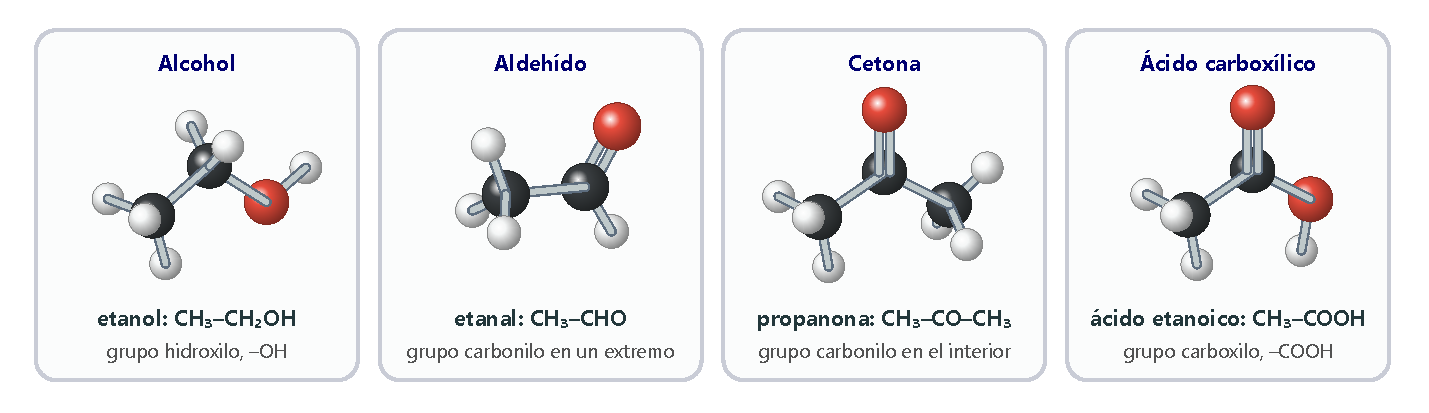
\includegraphics[width=\textwidth]{images/UD7/oxigenados}
    \caption{Modelos de bolas de los principales compuestos oxigenados de dos y tres carbonos.}
    \label{fig:ud7-oxigenados}
\end{figure}

\subsection{Alcoholes y fenoles}

Contienen el grupo \textbf{hidroxilo}, \ch{-OH}. En los \textbf{alcoholes} va unido a una cadena alifática (\ch{R-OH}), y en los
\textbf{fenoles}, a un anillo aromático (\ch{Ar-OH}). Los alcoholes son \textbf{primarios}, \textbf{secundarios} o
\textbf{terciarios} según el carbono que lleva el \ch{-OH}.

\paragraph{Nomenclatura.} Se añade el sufijo \textbf{-ol} al nombre del hidrocarburo, con el localizador del \ch{-OH} delante; con
varios grupos, \textbf{-diol}, \textbf{-triol}\ldots\ (polialcoholes, que conservan la «o» del hidrocarburo). Como sustituyente, el
\ch{-OH} se nombra \textbf{hidroxi-}.
\[ \underset{\text{etanol}}{\ch{CH3-CH2OH}} \qquad
   \underset{\text{3-metilbut-3-en-1-ol}}{\chemfig{CH_2=C(-[6]CH_3)-CH_2-CH_2OH}} \qquad
   \underset{\text{propano-1,2-diol}}{\ch{CH2OH-CHOH-CH3}} \]
Dos grupos \ch{-OH} no suelen estar en el mismo carbono, ni un \ch{-OH} en un carbono con doble enlace (esos compuestos son
inestables). En los fenoles se numera el anillo para que los \ch{-OH} tengan los localizadores más bajos:
\[ \underset{\text{fenol}}{\chemfig{*6(-=-=(-OH)-=)}} \qquad
   \underset{\text{benceno-1,3-diol}}{\chemfig{*6(-=(-OH)-=(-OH)-=)}} \qquad
   \underset{\text{4-metilfenol}}{\chemfig{*6(-=(-CH_3)-=-(-OH)=)}} \]

\paragraph{Propiedades y aplicaciones.} El grupo \ch{-OH} permite formar \textbf{enlaces de hidrógeno} entre moléculas
(figura~\ref{fig:ud7-hidrogeno}): por eso sus puntos de fusión y ebullición son mucho \textbf{más altos} que los de los
hidrocarburos de masa parecida, y los de menos carbonos son \textbf{solubles en agua}. La solubilidad disminuye al alargarse la
cadena, que es apolar. El \textbf{etanol} se obtiene por fermentación de azúcares y se usa como bebida, disolvente, desinfectante y
combustible (bioetanol); el \textbf{metanol} es muy tóxico; el \textbf{propan-2-ol} (alcohol isopropílico) limpia componentes
electrónicos, y la \textbf{glicerina} (propano-1,2,3-triol) se usa en cosmética.

\begin{figure}[H]
    \centering
    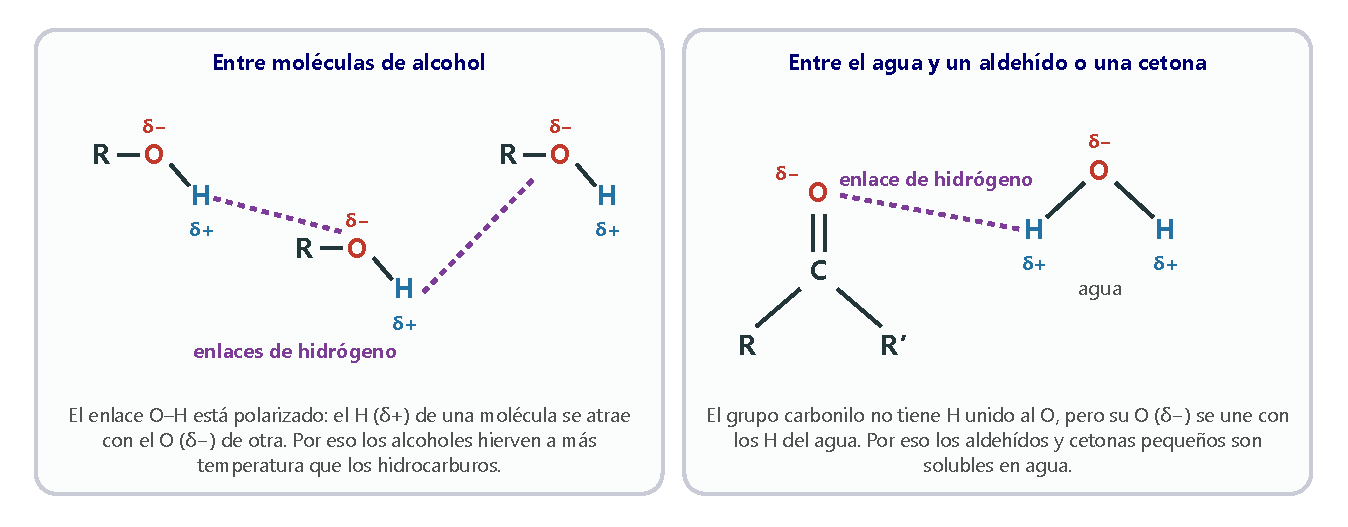
\includegraphics[width=0.95\textwidth]{images/UD7/enlace_hidrogeno}
    \caption{Enlaces de hidrógeno entre moléculas de alcohol y entre el agua y un compuesto con grupo carbonilo.}
    \label{fig:ud7-hidrogeno}
\end{figure}

\begin{exercise}
    Formula o nombra, e indica si los alcoholes son primarios, secundarios o terciarios: a) propan-2-ol; b) butano-1,3-diol; c)
    2-metilbutan-2-ol; d) but-3-en-1-ol; e) 3-metilfenol; f) \ch{CH3-CH2-CHOH-CH3}; g) \ch{CH2OH-CH2OH};
    h) \ch{CH2OH-CHOH-CH2OH}; i) \ch{CH3-CH=CH-CH2OH}.
    \begin{solu}
        a) \textcolor{red}{\ch{CH3-CHOH-CH3}, secundario}; b) \textcolor{red}{\ch{CH2OH-CH2-CHOH-CH3}, primario y secundario};
        c) \textcolor{red}{\chemfig{CH_3-C(-[2]OH)(-[6]CH_3)-CH_2-CH_3}, terciario}; d) \textcolor{red}{\ch{CH2=CH-CH2-CH2OH}, primario};
        e) \textcolor{red}{\chemfig{*6(-=(-CH_3)-=(-OH)-=)}}; f) \textcolor{red}{butan-2-ol, secundario};
        g) \textcolor{red}{etano-1,2-diol} (etilenglicol, anticongelante); h) \textcolor{red}{propano-1,2,3-triol} (glicerina);
        i) \textcolor{red}{but-2-en-1-ol, primario}.
    \end{solu}
\end{exercise}

\subsection{Éteres}

Su grupo funcional es un oxígeno unido a dos radicales: \ch{R-O-R'}. Se pueden nombrar de dos formas:
\begin{itemize}
    \item \textbf{Nombre de clase funcional}: los dos radicales en orden alfabético y la palabra \textbf{éter}:
    \ch{CH3-O-CH2-CH2-CH3}, metil propil éter.
    \item \textbf{Nomenclatura de sustitución} (la preferida por la IUPAC): el radical más sencillo con la terminación
    \textbf{-oxi} (\ch{CH3-O-}, metoxi; \ch{CH3-CH2-O-}, etoxi), seguido del nombre del hidrocarburo más complejo:
    \ch{CH3-O-CH2-CH2-CH3}, 1-metoxipropano.
\end{itemize}
Los éteres son poco reactivos y tienen puntos de ebullición más bajos que los alcoholes, porque no forman enlaces de hidrógeno entre
sus moléculas. Muchos son líquidos volátiles e inflamables que se usan como disolventes; el dietil éter fue uno de los primeros
anestésicos. Los \textbf{éteres corona}, cíclicos y con muchos oxígenos, atrapan cationes en su interior.

\begin{exercise}
    Formula o nombra de las dos formas: a) dietil éter; b) metoxibenceno; c) \ch{CH3-O-CH2-CH2-CH3}; d) \ch{CH3-CH2-O-CH=CH2};
    e) \chemfig{CH_3-CH_2-O-CH(-[6]CH_3)-CH_3}.
    \begin{solu}
        a) \textcolor{red}{\ch{CH3-CH2-O-CH2-CH3}, etoxietano}; b) \textcolor{red}{\ch{C6H5-O-CH3}, metil fenil éter} (anisol);
        c) \textcolor{red}{metil propil éter, 1-metoxipropano}; d) \textcolor{red}{etil vinil éter, etoxieteno};
        e) \textcolor{red}{etil isopropil éter, 2-etoxipropano}.
    \end{solu}
\end{exercise}

\subsection{Aldehídos y cetonas}

Ambos tienen el grupo \textbf{carbonilo}, \ch{C=O}.
\begin{itemize}
    \item En los \textbf{aldehídos} el carbonilo está en un \textbf{carbono terminal} (\ch{-CHO}). Se nombran con la terminación
    \textbf{-al}; no necesitan localizador, porque el \ch{-CHO} es siempre el C1: \ch{HCHO}, metanal (formaldehído);
    \ch{CH3-CH2-CHO}, propanal; \ch{OHC-CH2-CH2-CHO}, butanodial. Como sustituyente, \textbf{formil-} u \textbf{oxo-}.
    \item En las \textbf{cetonas} el carbonilo está en un \textbf{carbono intermedio} (\ch{-CO-}). Se nombran con la terminación
    \textbf{-ona} y el localizador más bajo posible: \ch{CH3-CO-CH3}, propanona (acetona); \ch{CH3-CO-CH2-CH2-CH3}, pentan-2-ona;
    \ch{CH3-CO-CH2-CO-CH2-CH3}, hexano-2,4-diona. Como sustituyente, \textbf{oxo-}. También se pueden nombrar citando los dos
    radicales y la palabra cetona: metil propil cetona.
\end{itemize}
En las fórmulas semidesarrolladas se escribe \ch{-OH} para los alcoholes y \ch{-CHO} para los aldehídos.

Por el grupo carbonilo, son compuestos \textbf{polares}: sus puntos de ebullición son más altos que los de los hidrocarburos, pero
menores que los de los alcoholes (no forman enlaces de hidrógeno entre sí, aunque sí con el agua, y por eso los pequeños son
solubles). Se obtienen oxidando alcoholes y se usan para fabricar resinas, plásticos, disolventes, pinturas y perfumes. La acetona
disuelve lacas y pinturas; el metanal (formol) conserva muestras biológicas.

\begin{remark}
    \textbf{Acetonemia.} Después de una fiebre o de pasar muchas horas sin comer, el organismo agota sus reservas de glucosa y
    obtiene energía de las grasas. En ese proceso se forma propanona, que se elimina por el aliento: por eso huele a acetona.
\end{remark}

\begin{exercise}
    Formula o nombra: a) etanal; b) butanona; c) 3-metilbutanal; d) pentan-3-ona; e) propenal; f) hexano-2,4-diona;
    g) \chemfig{CH_3-CH(-[6]CH_3)-CO-CH_3}; h) \ch{OHC-CH2-CH2-CHO}; i) \ch{C6H5-CHO}; j) \ch{CH3-CO-CH2-CH=CH2}.
    \begin{solu}
        a) \textcolor{red}{\ch{CH3-CHO}}; b) \textcolor{red}{\ch{CH3-CO-CH2-CH3}}; c) \textcolor{red}{\chemfig{CH_3-CH(-[6]CH_3)-CH_2-CHO}};
        d) \textcolor{red}{\ch{CH3-CH2-CO-CH2-CH3}}; e) \textcolor{red}{\ch{CH2=CH-CHO}}; f) \textcolor{red}{\ch{CH3-CO-CH2-CO-CH2-CH3}};
        g) \textcolor{red}{3-metilbutan-2-ona}; h) \textcolor{red}{butanodial}; i) \textcolor{red}{benzaldehído}
        (bencenocarbaldehído); j) \textcolor{blue}{la cetona tiene prioridad sobre el doble enlace:} \textcolor{red}{pent-4-en-2-ona}.
    \end{solu}
\end{exercise}

\subsection{Ácidos carboxílicos}

Su grupo funcional es el \textbf{carboxilo}, \ch{-COOH}, siempre en un extremo de la cadena. Se nombran con la palabra
\textbf{ácido} y la terminación \textbf{-oico}; el carbono del \ch{-COOH} es el C1:
\[ \underset{\text{ácido metanoico (fórmico)}}{\ch{HCOOH}} \qquad \underset{\text{ácido etanoico (acético)}}{\ch{CH3-COOH}}
   \qquad \underset{\text{ácido propanodioico}}{\ch{HOOC-CH2-COOH}} \qquad \underset{\text{ácido benzoico}}{\ch{C6H5-COOH}} \]

Son sustancias \textbf{polares} que forman enlaces de hidrógeno muy fuertes entre sí: sus puntos de ebullición son mayores que los
de los alcoholes. Los primeros de la serie son solubles en agua. Son \textbf{ácidos débiles} con muchas aplicaciones en la industria
\textbf{alimentaria} (vinagre, conservantes, acidulantes) y \textbf{farmacéutica}: el ácido acetilsalicílico es la aspirina.

\begin{exercise}
    Formula o nombra: a) ácido butanoico; b) ácido 2-metilpropanoico; c) ácido but-2-enoico; d) ácido etanodioico (oxálico); e)
    \chemfig{CH_3-CH_2-CH(-[6]CH_3)-COOH}; f) \ch{CH2=CH-COOH}; g) \ch{HOOC-CH2-CH2-COOH}.
    \begin{solu}
        a) \textcolor{red}{\ch{CH3-CH2-CH2-COOH}}; b) \textcolor{red}{\chemfig{CH_3-CH(-[6]CH_3)-COOH}};
        c) \textcolor{red}{\ch{CH3-CH=CH-COOH}}; d) \textcolor{red}{\ch{HOOC-COOH}}; e) \textcolor{red}{ácido 2-metilbutanoico};
        f) \textcolor{red}{ácido propenoico} (acrílico); g) \textcolor{red}{ácido butanodioico} (succínico).
    \end{solu}
\end{exercise}

\subsection{Ésteres y sales}

Los \textbf{ésteres} resultan de sustituir el H del grupo carboxilo por un radical: \ch{R-COO-R'}. Se forman al reaccionar un
ácido con un alcohol (\textbf{esterificación}):
\[ \ch{CH3-COOH + HO-CH2-CH3 <=> CH3-COO-CH2-CH3 + H2O} \]
Se nombran cambiando la terminación -oico del ácido por \textbf{-oato}, seguida de \textbf{de} y el nombre del radical acabado en
\textbf{-ilo}: \ch{CH3-COO-CH2-CH3}, etanoato de etilo (acetato de etilo); \ch{CH3-CH2-CH2-COO-CH3}, butanoato de metilo.

Los ésteres de baja masa molecular son líquidos volátiles de \textbf{olor agradable} a frutas o flores, que se usan en perfumes y
aromas alimentarios; los de masa alta son sólidos, como las ceras y las grasas.

Si el H del carboxilo se sustituye por un metal se obtienen \textbf{sales}, que se nombran como los ésteres con el nombre del
metal: \ch{CH3-COONa}, etanoato de sodio; \ch{CH3-CH2-COOK}, propanoato de potasio. Los \textbf{jabones} son sales de sodio o
potasio de ácidos de cadena larga.

\begin{exercise}
    Formula o nombra: a) etanoato de metilo; b) metanoato de etilo; c) propanoato de propilo; d) benzoato de metilo;
    e) butanoato de sodio; f) \ch{CH3-COO-CH2-CH2-CH3}; g) \ch{CH3-CH2-COO-CH3}; h) \ch{HCOOK}; i) \ch{CH3-COO-C6H5}.
    \begin{solu}
        a) \textcolor{red}{\ch{CH3-COO-CH3}}; b) \textcolor{red}{\ch{HCOO-CH2-CH3}}; c) \textcolor{red}{\ch{CH3-CH2-COO-CH2-CH2-CH3}};
        d) \textcolor{red}{\ch{C6H5-COO-CH3}}; e) \textcolor{red}{\ch{CH3-CH2-CH2-COONa}}; f) \textcolor{red}{etanoato de propilo}
        (aroma de pera); g) \textcolor{red}{propanoato de metilo}; h) \textcolor{red}{metanoato de potasio};
        i) \textcolor{red}{etanoato de fenilo}.
    \end{solu}
\end{exercise}

%========================================================================================
\section{Compuestos nitrogenados}\label{sec:ud7-nitrogenados}
%========================================================================================

\subsection{Aminas}

Derivan del \textbf{amoníaco}, \ch{NH3}, al sustituir uno, dos o tres hidrógenos por radicales: son aminas \textbf{primarias}
(\ch{R-NH2}), \textbf{secundarias} (\ch{R-NH-R'}) o \textbf{terciarias} (figura~\ref{fig:ud7-aminas}).
\begin{itemize}
    \item \textbf{Primarias}: se cambia la -o final del hidrocarburo por \textbf{-amina}: \ch{CH3-NH2}, metanamina;
    \ch{CH3-CH2-CH2-NH2}, propan-1-amina.
    \item \textbf{Secundarias y terciarias}: se toma como cadena principal el radical más complejo y los demás se nombran como
    sustituyentes precedidos de \textbf{N-}: \ch{CH3-NH-CH2-CH3}, N-metiletanamina; \ch{(CH3)2N-CH2-CH2-CH2-CH3},
    N,N-dimetilbutan-1-amina.
    \item Como sustituyente, el grupo \ch{-NH2} se llama \textbf{amino-}. La amina aromática más sencilla, \ch{C6H5-NH2}, es la
    \textbf{anilina} (fenilamina o bencenamina).
\end{itemize}

\begin{figure}[H]
    \centering
    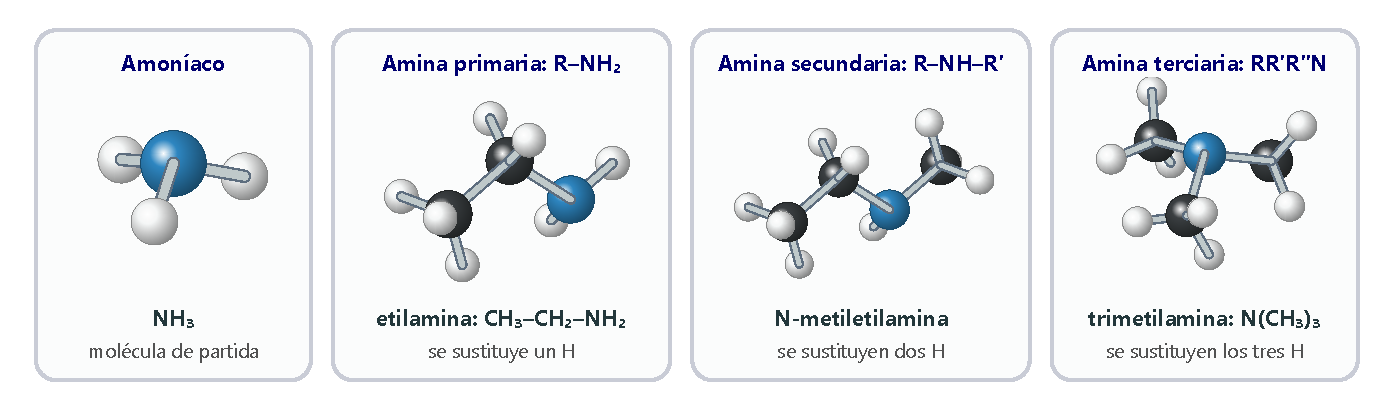
\includegraphics[width=\textwidth]{images/UD7/aminas}
    \caption{El amoníaco y las aminas primarias, secundarias y terciarias.}
    \label{fig:ud7-aminas}
\end{figure}

Por la polaridad del enlace \ch{N-H}, las aminas de baja masa molecular son solubles en agua. Son \textbf{bases}, con olor a
pescado podrido, que reaccionan fácilmente con los ácidos. Se usan para fabricar detergentes, colorantes y fármacos.

\subsection{Amidas}

Resultan de sustituir el \ch{-OH} de un ácido carboxílico por un grupo amino: \ch{R-CONH2}.
\begin{itemize}
    \item \textbf{Primarias}: se cambia la terminación -oico del ácido por \textbf{-amida}: \ch{CH3-CH2-CONH2}, propanamida.
    \item \textbf{Secundarias y terciarias}: se anteponen los radicales unidos al nitrógeno precedidos de \textbf{N-}:
    \ch{CH3-CO-NH-CH2-CH3}, N-etiletanamida; \ch{CH3-CO-N(CH3)-CH2-CH2-CH3}, N-metil-N-propiletanamida.
\end{itemize}
Las amidas son bases muy débiles y sustancias estables; salvo la metanamida, son \textbf{sólidas} a temperatura ambiente. Son muy
comunes en la naturaleza: las proteínas están formadas por aminoácidos unidos por enlaces de tipo amida (\textbf{enlace
peptídico}), y el \textbf{nailon} es una poliamida sintética.

\subsection{Nitrilos}

Tienen el grupo \ch{-C+N} en un extremo de la cadena. Se nombran con la terminación \textbf{-nitrilo}, contando el carbono del
grupo: \ch{CH3-C+N}, etanonitrilo (acetonitrilo); \ch{CH3-CH2-CH2-C+N}, butanonitrilo. Como sustituyente, \textbf{ciano-}. El
propenonitrilo (acrilonitrilo) es el monómero de fibras acrílicas.

\begin{example}
    \textbf{Compuestos nitrogenados.} a) Formula la N,N-dimetilpropanamida y la propan-2-amina. b) Nombra \ch{CH3-CH2-NH-CH2-CH3}
    y \ch{CH3-CH2-CH2-CH2-CONH2}.

    \textbf{Solución.} a) \ch{CH3-CH2-CO-N(CH3)2}: amida de tres carbonos con dos metilos en el N. \ch{CH3-CH(NH2)-CH3}: amina
    primaria con el \ch{-NH2} en el C2. b) Amina secundaria con dos etilos: \textbf{N-etiletanamina} (dietilamina). Amida primaria de
    5 carbonos: \textbf{pentanamida}.
\end{example}

\begin{exercise}
    Formula o nombra: a) etanamina; b) N-metilpropan-1-amina; c) N,N-dimetiletanamina; d) etanamida; e) N-metilbutanamida;
    f) fenilamina; g) \ch{H2N-CH2-CH2-NH2}; h) \ch{CH3-CO-N(CH3)2}; i) \ch{CH3-CH2-C+N}; j) \ch{CH3-CH2-N(CH3)-CH3}.
    \begin{solu}
        a) \textcolor{red}{\ch{CH3-CH2-NH2}}; b) \textcolor{red}{\ch{CH3-NH-CH2-CH2-CH3}}; c) \textcolor{red}{\ch{(CH3)2N-CH2-CH3}};
        d) \textcolor{red}{\ch{CH3-CONH2}}; e) \textcolor{red}{\ch{CH3-CH2-CH2-CO-NH-CH3}}; f) \textcolor{red}{\ch{C6H5-NH2}};
        g) \textcolor{red}{etano-1,2-diamina}; h) \textcolor{red}{N,N-dimetiletanamida}; i) \textcolor{red}{propanonitrilo};
        j) \textcolor{red}{N,N-dimetiletanamina}.
    \end{solu}
\end{exercise}

%========================================================================================
\section{Compuestos con varios grupos funcionales}\label{sec:ud7-varios}
%========================================================================================

Cuando hay más de un grupo funcional, se aplica la tabla~\ref{tab:ud7-prioridad}: el de mayor prioridad se nombra con su sufijo y
los demás, como prefijos, en orden alfabético con las ramificaciones y los halógenos.

\begin{example}
    \textbf{Nombrar un compuesto con varios grupos.} Nombra \chemfig{CH_3-CO-CH_2-CH(-[6]CH_3)-COOH}.

    \textbf{Solución.} 1) Grupos: \ch{-COOH} (ácido) y \ch{-CO-} (cetona). El ácido tiene prioridad: sufijo \emph{-oico}; la cetona
    será el prefijo \emph{oxo-}. 2) Cadena principal: 5 carbonos, numerados desde el \ch{-COOH} (C1). 3) Sustituyentes: metilo en
    C2 y oxo en C4. 4) Por orden alfabético (m antes que o): \textbf{ácido 2-metil-4-oxopentanoico}.
\end{example}

\begin{example}
    \textbf{Formular un compuesto con varios grupos.} Formula la 4-hidroxi-3-metilbutan-2-ona.

    \textbf{Solución.} El sufijo \emph{-ona} indica que la cetona es el grupo principal, en el C2 de una cadena de 4 carbonos. El
    \ch{-OH} (hidroxi) va en el C4 y un metilo en el C3:
    \[ \chemfig{CH_3-CO-CH(-[6]CH_3)-CH_2OH} \]
\end{example}

\begin{exercise}
    Formula o nombra: a) 2-hidroxipropanal; b) ácido 2-aminopropanoico (alanina); c) 4-oxopentanal; d) 3-hidroxibutan-2-ona;
    e) \ch{HOCH2-CH2-COOH}; f) \ch{CH3-CO-CH2-COOH}; g) \ch{H2N-CH2-CH2OH}; h) \ch{CH2=CH-CO-CH3}.
    \begin{solu}
        a) \textcolor{red}{\ch{CH3-CHOH-CHO}}; b) \textcolor{red}{\ch{CH3-CH(NH2)-COOH}}; c) \textcolor{red}{\ch{CH3-CO-CH2-CH2-CHO}};
        d) \textcolor{red}{\ch{CH3-CO-CHOH-CH3}}; e) \textcolor{red}{ácido 3-hidroxipropanoico}; f) \textcolor{red}{ácido
        3-oxobutanoico}; g) \textcolor{blue}{el alcohol tiene prioridad sobre la amina:} \textcolor{red}{2-aminoetanol};
        h) \textcolor{red}{but-3-en-2-ona}.
    \end{solu}
\end{exercise}

%========================================================================================
\section{Isomería}\label{sec:ud7-isomeria}
%========================================================================================

\begin{definition}[Isomería]
    Es la propiedad de los compuestos que tienen la \textbf{misma fórmula molecular} pero \textbf{distinta estructura}, y por tanto
    distintas propiedades. Estos compuestos se llaman \textbf{isómeros}.
\end{definition}

\subsection{Isomería estructural}

Los isómeros estructurales se diferencian en las \textbf{uniones} entre sus átomos:
\begin{itemize}
    \item \textbf{De cadena}: distinta cadena carbonada. \ch{C4H10}: butano, \ch{CH3-CH2-CH2-CH3}, y metilpropano,
    \chemfig{CH_3-CH(-[6]CH_3)-CH_3}.
    \item \textbf{De posición}: el mismo grupo funcional (o enlace múltiple) en distinta posición. \ch{C5H10O}: pentan-2-ona,
    \ch{CH3-CO-CH2-CH2-CH3}, y pentan-3-ona, \ch{CH3-CH2-CO-CH2-CH3}.
    \item \textbf{De función}: distinto grupo funcional. \ch{C4H10O}: butan-2-ol, \ch{CH3-CHOH-CH2-CH3}, y dietil éter,
    \ch{CH3-CH2-O-CH2-CH3}. Son pares típicos los alcoholes y los éteres, los aldehídos y las cetonas o los ácidos y los ésteres.
\end{itemize}

\subsection{Estereoisomería}

Los \textbf{estereoisómeros} tienen la misma fórmula molecular y la misma estructura (los mismos enlaces), pero sus átomos están
\textbf{distribuidos en el espacio} de distinta forma.

\paragraph{Isomería geométrica o cis-trans.} Aparece en compuestos con un doble enlace, porque este impide la rotación de los
carbonos que une. Si cada carbono del doble enlace tiene dos sustituyentes \textbf{distintos}, hay dos isómeros: \textbf{cis}, con
los grupos más voluminosos al mismo lado, y \textbf{trans}, en lados opuestos.
\[ \underset{\text{\emph{cis}-but-2-eno}}{\chemfig{C(-[3]H_3C)(-[5]H)=C(-[1]CH_3)(-[7]H)}} \qquad\qquad
   \underset{\text{\emph{trans}-but-2-eno}}{\chemfig{C(-[3]H_3C)(-[5]H)=C(-[1]H)(-[7]CH_3)}} \]
El but-1-eno, \ch{CH2=CH-CH2-CH3}, no tiene isómeros cis-trans: uno de sus carbonos tiene dos H iguales.

\paragraph{Isomería óptica.} La presentan las moléculas con un \textbf{carbono asimétrico} o \textbf{quiral}, unido a cuatro
sustituyentes distintos (se marca con un asterisco). Hay dos isómeros, los \textbf{enantiómeros}, que son imágenes especulares no
superponibles, como nuestras manos (figura~\ref{fig:ud7-enantiomeros}). Tienen casi todas las propiedades iguales, pero desvían
el plano de la luz polarizada en sentidos opuestos y actúan de forma distinta en los seres vivos: de muchos fármacos, como el
ibuprofeno, solo uno de los enantiómeros es activo.

\begin{figure}[H]
    \centering
    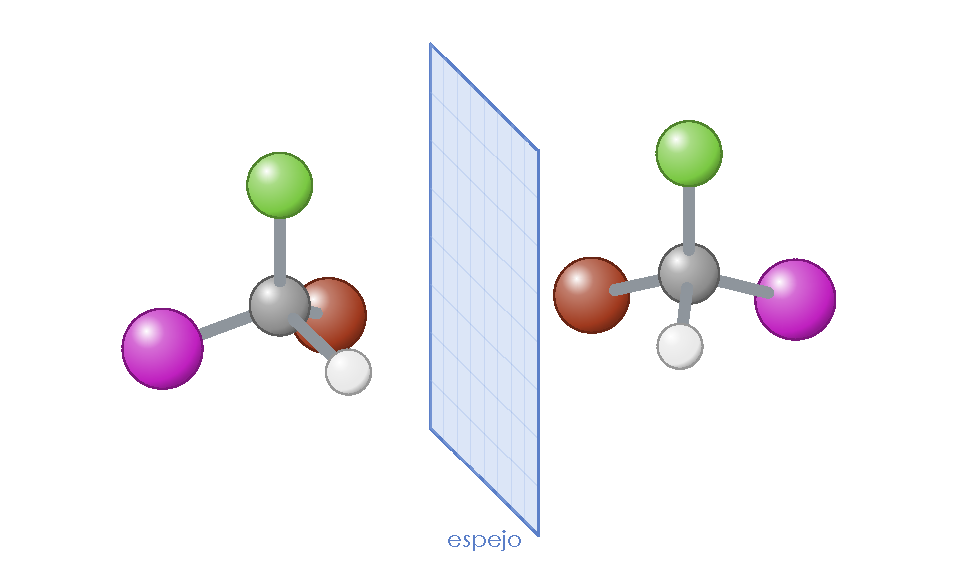
\includegraphics[width=0.55\textwidth]{images/UD7/enantiomeros}
    \caption{Dos enantiómeros: un carbono con cuatro sustituyentes distintos y su imagen en un espejo no se pueden superponer.}
    \label{fig:ud7-enantiomeros}
\end{figure}

\begin{example}
    \textbf{Buscar isómeros.} Escribe y nombra todos los isómeros de fórmula \ch{C3H8O}. ¿Qué tipo de isomería hay entre ellos?

    \textbf{Solución.} Con un \ch{-OH}: propan-1-ol, \ch{CH3-CH2-CH2OH}, y propan-2-ol, \ch{CH3-CHOH-CH3} (isómeros de
    \textbf{posición}). Con un \ch{-O-}: etil metil éter (metoxietano), \ch{CH3-O-CH2-CH3}, isómero de \textbf{función} de los dos
    alcoholes. Ninguno tiene carbono quiral ni doble enlace, así que no hay estereoisómeros.
\end{example}

\begin{exercise}
    Escribe y nombra los tres isómeros de cadena del \ch{C5H12} y los cinco hidrocarburos de cadena abierta de fórmula \ch{C6H14}.
    \begin{solu}
        \textcolor{red}{\ch{C5H12}: pentano, 2-metilbutano y 2,2-dimetilpropano.} \textcolor{red}{\ch{C6H14}: hexano,
        2-metilpentano, 3-metilpentano, 2,2-dimetilbutano y 2,3-dimetilbutano.}
    \end{solu}
\end{exercise}

\begin{exercise}
    Escribe dos isómeros de posición del \ch{C4H8} con un doble enlace y dos isómeros de función de fórmula \ch{C3H6O}.
    \begin{solu}
        \textcolor{red}{But-1-eno, \ch{CH2=CH-CH2-CH3}, y but-2-eno, \ch{CH3-CH=CH-CH3}.} \textcolor{red}{Propanal,
        \ch{CH3-CH2-CHO}, y propanona, \ch{CH3-CO-CH3}} (también el prop-2-en-1-ol, \ch{CH2=CH-CH2OH}).
    \end{solu}
\end{exercise}

\begin{exercise}
    ¿Cuáles presentan isomería cis-trans? Dibuja los dos isómeros cuando existan: a) propeno; b) pent-2-eno; c)
    2-metilbut-2-eno; d) 1,2-dicloroeteno.
    \begin{solu}
        a) \textcolor{red}{No} (el C1 tiene dos H). b) \textcolor{red}{Sí}: \chemfig{C(-[3]H_3C)(-[5]H)=C(-[1]CH_2-CH_3)(-[7]H)} (cis) y
        \chemfig{C(-[3]H_3C)(-[5]H)=C(-[1]H)(-[7]CH_2-CH_3)} (trans). c) \textcolor{red}{No} (el C2 tiene dos metilos). d)
        \textcolor{red}{Sí}: \chemfig{C(-[3]Cl)(-[5]H)=C(-[1]Cl)(-[7]H)} (cis) y \chemfig{C(-[3]Cl)(-[5]H)=C(-[1]H)(-[7]Cl)} (trans).
    \end{solu}
\end{exercise}

\begin{exercise}
    ¿Cuáles tienen un carbono quiral? Señálalo. a) Butan-2-ol; b) propan-2-ol; c) ácido 2-hidroxipropanoico (láctico); d)
    2-clorobutano; e) 3-metilpentano.
    \begin{solu}
        a) \textcolor{red}{Sí}, el C2 de \ch{CH3-CHOH-CH2-CH3}, unido a H, OH, \ch{CH3} y \ch{C2H5}. b) \textcolor{red}{No}: dos metilos iguales.
        c) \textcolor{red}{Sí}, el C2: H, OH, \ch{CH3} y \ch{COOH}. d) \textcolor{red}{Sí}, el C2. e) \textcolor{red}{No}: el C3
        tiene dos etilos iguales.
    \end{solu}
\end{exercise}

%========================================================================================
\section{Importancia de los compuestos del carbono}\label{sec:ud7-importancia}
%========================================================================================

\subsection{El petróleo y la industria petroquímica}

El \textbf{petróleo} es un líquido aceitoso, viscoso e inflamable, menos denso que el agua, formado por una mezcla de
\textbf{hidrocarburos} con pequeñas cantidades de compuestos de azufre, oxígeno y nitrógeno. Se formó durante millones de años a
partir de restos de plancton y algas enterrados a gran presión y temperatura, y se acumula en \textbf{yacimientos}. Una vez
extraído, el crudo se \textbf{refina}:
\begin{itemize}
    \item \textbf{Destilación fraccionada}: se calienta y se separa en fracciones según su temperatura de ebullición
    (figura~\ref{fig:ud7-destilacion}). Las de menos carbonos salen por arriba y las más pesadas, por abajo.
    \item \textbf{Transformaciones químicas}: el \textbf{craqueo} rompe los hidrocarburos pesados en otros más ligeros y en
    \textbf{olefinas} (alquenos como el eteno y el propeno), materia prima de los plásticos.
\end{itemize}

\begin{figure}[H]
    \centering
    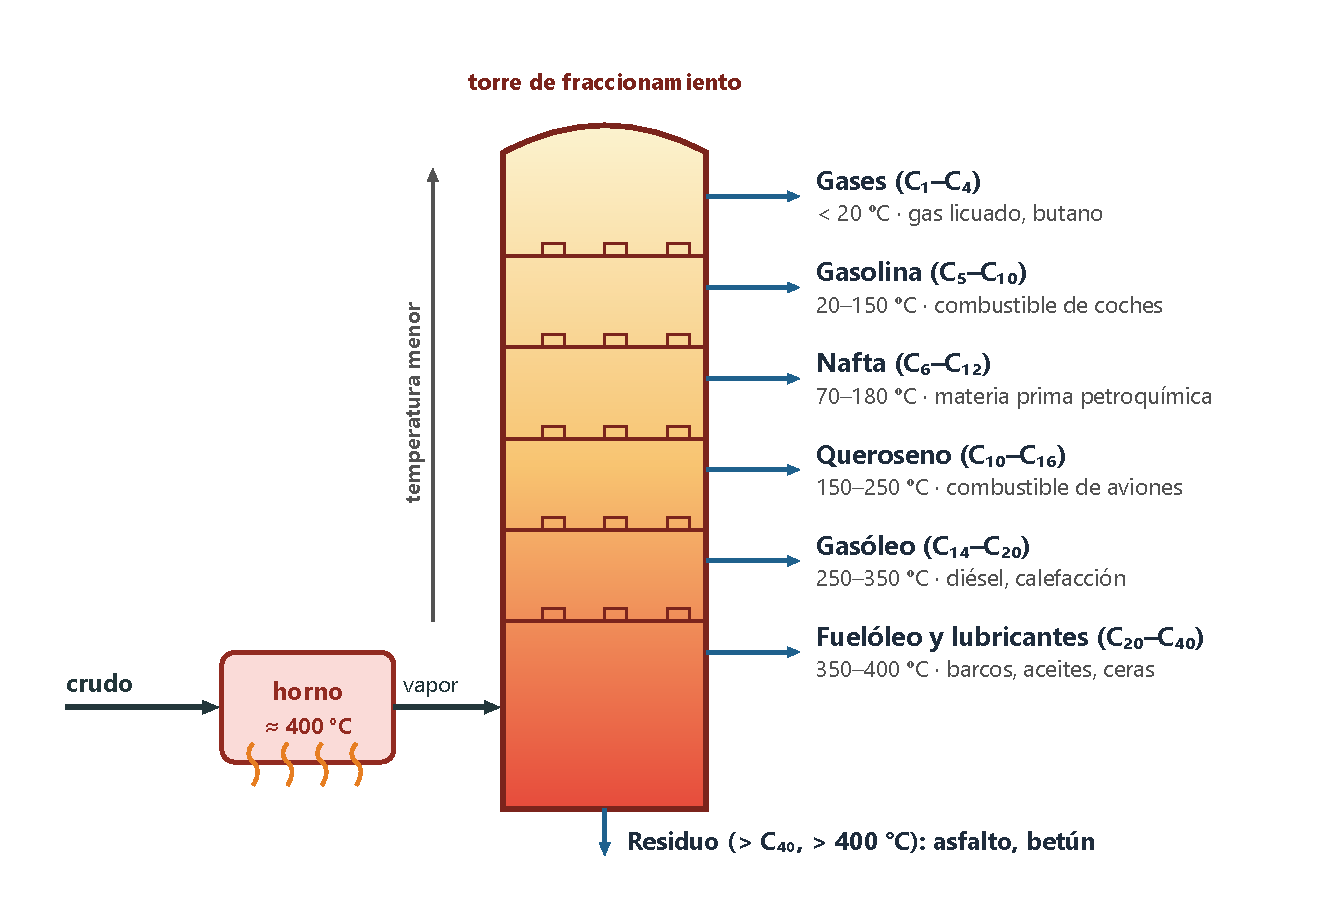
\includegraphics[width=0.85\textwidth]{images/UD7/torre_destilacion}
    \caption{Destilación fraccionada del petróleo.}
    \label{fig:ud7-destilacion}
\end{figure}

La \textbf{industria petroquímica} convierte estos productos en materias primas para fabricar plásticos, fibras sintéticas,
detergentes, anticongelantes, pinturas o fármacos: hasta un 60\,\% de los productos del mercado dependen de ella. Pero la
explotación del petróleo tiene un fuerte \textbf{impacto ambiental}: contaminación del suelo, el agua y el aire por derrames y
residuos (como la «marea negra» del \emph{Prestige} en Galicia, en 2002), deforestación para construir plataformas, carreteras y
oleoductos y, sobre todo, las emisiones de \ch{CO2} de su combustión, causa principal del cambio climático.

\subsection{Compuestos orgánicos de síntesis}

\begin{definition}[Síntesis orgánica]
    Es la construcción planificada de moléculas orgánicas complejas a partir de otras más sencillas mediante reacciones químicas.
\end{definition}

Desde la síntesis de la urea se han fabricado millones de moléculas: unas existen en la naturaleza y otras se han diseñado con un
fin concreto. Sus campos principales son los fármacos y los polímeros.

\paragraph{Síntesis de fármacos.} Fabricar un medicamento es un proceso largo en el que la primera etapa es obtener el
\textbf{principio activo}. Puede hacerse por \textbf{síntesis total}, a partir de sustancias sencillas y baratas, o por
\textbf{síntesis parcial}, partiendo de un compuesto extraído de la naturaleza. Para diseñar la ruta se usa el \textbf{análisis
retrosintético} de \textbf{E. J. Corey}: «desmontar» mentalmente la molécula objetivo en piezas cada vez más sencillas. El premio
Nobel de Química de 2022 fue para \textbf{B. Sharpless} y \textbf{M. Meldal}, por la \textbf{química clic}, que une bloques
moleculares de forma rápida y limpia, y para \textbf{C. Bertozzi}, que la llevó al interior de los organismos vivos.

\paragraph{Polímeros.} Los \textbf{polímeros} son macromoléculas formadas por la unión de muchas moléculas pequeñas, los
\textbf{monómeros}. Pueden ser \textbf{naturales} (celulosa, almidón, proteínas, caucho) o \textbf{sintéticos} (polietileno, PVC,
nailon, neopreno). La \textbf{polimerización} puede ser:
\begin{itemize}
    \item \textbf{por adición}: los monómeros, con un doble enlace, se unen sin perder átomos. Así se obtiene el
    \textbf{polietileno} a partir del eteno (figura~\ref{fig:ud7-polietileno}): \(n\,\ch{CH2=CH2} \rightarrow (\ch{-CH2-CH2-})_n\);
    \item \textbf{por condensación}: al unirse los monómeros se desprende una molécula pequeña, normalmente agua. Así se forman
    el nailon, el poliéster (PET) o las proteínas.
\end{itemize}
Los polímeros sintéticos son ligeros, fáciles de moldear, resistentes a la corrosión y aislantes. Se clasifican en
\textbf{plásticos}, \textbf{fibras} (nailon, poliéster) y \textbf{elastómeros} (neopreno, caucho sintético).

\begin{figure}[H]
    \centering
    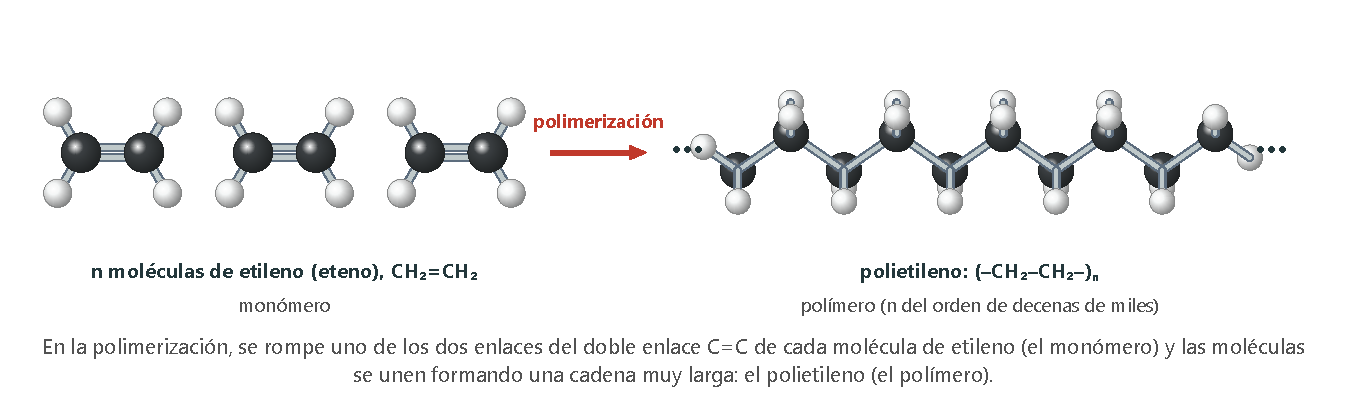
\includegraphics[width=0.9\textwidth]{images/UD7/polietileno}
    \caption{Polimerización por adición del eteno para dar polietileno.}
    \label{fig:ud7-polietileno}
\end{figure}

\subsection{Los compuestos orgánicos en los seres vivos}

Los seres vivos estamos formados en un 99\,\% por C, H, O, N, S y P, los \textbf{bioelementos} principales, que forman las
\textbf{biomoléculas}. La estructura de cada una determina su función:
\begin{itemize}
    \item \textbf{Glúcidos}: formados por C, H y O. Tienen función \textbf{energética} (la glucosa se «quema» en la respiración
    celular; el almidón y el glucógeno son reservas) y \textbf{estructural} (la celulosa de las paredes vegetales). Los
    monosacáridos, como la glucosa o la fructosa, se unen por condensación en disacáridos (la lactosa de la leche) y polisacáridos.
    \item \textbf{Lípidos}: insolubles en agua. Forman las membranas celulares y almacenan energía. Las \textbf{grasas saturadas}
    (mantequilla, embutidos) elevan el colesterol LDL y el riesgo cardiovascular; las \textbf{insaturadas} (aceite de oliva,
    pescado azul) ayudan a reducirlo.
    \item \textbf{Proteínas}: macromoléculas formadas por \textbf{aminoácidos}, compuestos con un grupo amino y un grupo ácido. Los
    aminoácidos se unen por condensación mediante el \textbf{enlace peptídico} (un enlace amida):
    \begin{gather*} \ch{H2N-CH2-COOH + H2N-CH(CH3)-COOH} \\ \ch{-> H2N-CH2-CO-NH-CH(CH3)-COOH + H2O} \end{gather*}
    Tienen funciones de transporte (hemoglobina), estructura (colágeno), hormonales (insulina), defensa (anticuerpos), movimiento
    (miosina) o catálisis (enzimas).
    \item \textbf{Ácidos nucleicos} (ADN y ARN), que almacenan y transmiten la información genética, y \textbf{vitaminas}, necesarias
    en pequeñas cantidades.
\end{itemize}

\begin{exercise}
    a) Escribe un fragmento de tres unidades del polipropileno, que se obtiene por adición del propeno. b) ¿Cuál es la masa molar de
    una cadena formada por \num{5000} monómeros?
    \begin{solu}
        a) \textcolor{red}{\ch{-CH2-CH(CH3)-CH2-CH(CH3)-CH2-CH(CH3)-}}: el doble enlace se abre y los metilos quedan como
        ramificaciones. b) \(M = 5000 \cdot 42 = \textcolor{red}{\qty{2.1e5}{\gram\per\mol}}\).
    \end{solu}
\end{exercise}

\begin{exercise}
    En el dipéptido de la ecuación anterior (glicina + alanina), señala el enlace peptídico, el grupo amino libre y el grupo
    carboxilo libre. ¿Qué tipo de reacción es? ¿Qué grupo funcional orgánico forma el enlace peptídico?
    \begin{solu}
        \textcolor{red}{El enlace peptídico es el \ch{-CO-NH-} central; el \ch{-NH2} libre está en el extremo de la glicina y el
        \ch{-COOH} libre, en el de la alanina.} Es una \textcolor{red}{condensación} (se desprende agua) y el enlace es una
        \textcolor{red}{amida}.
    \end{solu}
\end{exercise}

\begin{exercise}
    a) ¿Por qué el queroseno sale de la torre de destilación por encima del gasóleo? b) ¿Qué es el craqueo y para qué sirve? c) Cita
    tres impactos ambientales de la explotación del petróleo.
    \begin{solu}
        a) \textcolor{red}{Sus hidrocarburos son más pequeños (\ch{C10}--\ch{C16}) y tienen menor punto de ebullición}: condensan a
        menor temperatura, más arriba. b) \textcolor{red}{Romper con calor (y catalizadores) hidrocarburos pesados en otros más
        ligeros}, para obtener más gasolina y alquenos para la petroquímica. c) \textcolor{red}{Derrames que contaminan mares y
        costas, contaminación del aire y del suelo en las refinerías, deforestación y emisiones de \ch{CO2}} (cambio climático).
    \end{solu}
\end{exercise}

%========================================================================================
\section{Química en la vida: las mil caras del carbono}\label{sec:ud7-alotropos}
%========================================================================================

El carbono puro existe en varias formas, sus \textbf{alótropos}, con propiedades muy distintas. En el \textbf{diamante} cada átomo
está unido a otros cuatro en una red tridimensional rígida: es transparente, aislante y el material natural más duro. En el
\textbf{grafito} los átomos forman láminas de hexágonos apiladas, que se deslizan unas sobre otras: es blando, negro y conduce la
electricidad, porque cada carbono tiene un electrón deslocalizado.

En 1985, \textbf{H. Kroto}, \textbf{R. Curl} y \textbf{R. Smalley} descubrieron los \textbf{fullerenos}, moléculas huecas como el
\ch{C60}, con forma de balón de fútbol (premio Nobel de Química de 1996). En 1991, \textbf{S. Iijima} describió los
\textbf{nanotubos de carbono}, láminas de grafito enrolladas en cilindros, cien veces más resistentes que el acero y muy ligeros.
Y en 2004, \textbf{A. Geim} y \textbf{K. Novoselov} aislaron el \textbf{grafeno} pegando y despegando cinta adhesiva sobre un trozo
de grafito (premio Nobel de Física de 2010): una lámina de un solo átomo de grosor, flexible, transparente, más resistente que el
acero y mejor conductora que el cobre.

Estos materiales prometen pantallas flexibles, baterías de carga rápida, sensores, placas solares más eficientes, filtros para
potabilizar agua o transportar fármacos dentro del cuerpo. Todo, con el mismo elemento que forma la mina de un lápiz.

\begin{exercise}
    a) ¿Qué son los alótropos? b) ¿Por qué el grafito conduce la electricidad y el diamante no? c) El \ch{C60} tiene 60 átomos de
    carbono. ¿Cuál es su masa molar? ¿Cuántas moléculas hay en \qty{1}{\milli\gram}?
    \begin{solu}
        a) \textcolor{red}{Formas distintas de un mismo elemento}, con distinta estructura y propiedades. b) \textcolor{red}{En el
        grafito cada C se une solo a otros tres y le queda un electrón deslocalizado que puede moverse por la lámina}; en el diamante
        los cuatro electrones de valencia están en enlaces localizados. c) \(M = 60 \cdot 12 = \textcolor{red}{\qty{720}{\gram\per\mol}}\);
        \(N = \dfrac{\num{1e-3}}{720} \cdot \num{6.02e23} = \textcolor{red}{\num{8.4e17}}\) moléculas.
    \end{solu}
\end{exercise}

%========================================================================================
\section{Prácticas}\label{sec:ud7-practicas}
%========================================================================================

\subsection{Modelos moleculares con plastilina: isómeros}

\noindent\begin{minipage}[t]{0.48\textwidth}
    \textbf{Objetivo}
    \begin{itemize}
        \item Construir modelos de moléculas orgánicas para ver su forma en el espacio y comprobar que fórmulas moleculares iguales
        pueden dar estructuras distintas.
    \end{itemize}
\end{minipage}\hfill
\begin{minipage}[t]{0.48\textwidth}
    \textbf{Material}
    \begin{itemize}
        \item Plastilina de cuatro colores (negro para C, blanco para H, rojo para O y verde para Cl).
        \item Palillos de dientes y un transportador de ángulos.
    \end{itemize}
\end{minipage}

\textbf{Procedimiento}
\begin{enumerate}[label=\numberballgreen]
    \item Haz bolas de plastilina: las de C, algo más grandes que las de H.
    \item Construye el metano clavando cuatro palillos en una bola negra de forma que estén lo más separados posible. Mide el ángulo
    entre dos palillos.
    \item Construye el butano y el metilpropano (\ch{C4H10}). Gira los enlaces sencillos del butano: ¿cambia la molécula?
    \item Construye los dos isómeros del \ch{C2H6O}: el etanol y el dimetil éter.
    \item Para los dobles enlaces, une dos carbonos con dos palillos y construye el \emph{cis}- y el
    \emph{trans}-1,2-dicloroeteno. Intenta girar el doble enlace.
\end{enumerate}

\begin{exercise}
    a) ¿Qué ángulo aproximado has medido en el metano? ¿Cuál es el teórico? b) ¿Por qué girar los enlaces del butano no da un
    isómero nuevo y en el 1,2-dicloroeteno sí hay dos isómeros? c) Construye todos los isómeros del \ch{C3H6Cl2} y nómbralos.
    \begin{solu}
        a) \textcolor{red}{Unos \ang{110}; el teórico es \ang{109.5}}. b) \textcolor{red}{Los enlaces sencillos giran libremente:
        las distintas posiciones son la misma molécula. El doble enlace no puede girar}, así que los Cl quedan fijos al mismo lado o
        en lados opuestos. c) \textcolor{red}{1,1-dicloropropano, 1,2-dicloropropano, 1,3-dicloropropano y 2,2-dicloropropano}
        (el 1,2- tiene además un carbono quiral).
    \end{solu}
\end{exercise}

\subsection{Química en la cocina: fruta caramelizada}

\noindent\begin{minipage}[t]{0.48\textwidth}
    \textbf{Objetivo}
    \begin{itemize}
        \item Observar la \textbf{caramelización} del azúcar, una serie de reacciones de descomposición de la sacarosa por el calor, y
        preparar un tentempié de fruta.
    \end{itemize}
\end{minipage}\hfill
\begin{minipage}[t]{0.48\textwidth}
    \textbf{Material}
    \begin{itemize}
        \item \qty{150}{\gram} de fruta (manzana, pera, plátano\ldots), \qty{300}{\gram} de azúcar moreno o panela, una cucharada de
        miel y \qty{25}{\gram} de mantequilla.
        \item Sartén antiadherente, espátula, termómetro de cocina y papel de horno.
    \end{itemize}
\end{minipage}

\textbf{Procedimiento}
\begin{enumerate}[label=\numberballgreen]
    \item Lava la fruta, quítale las semillas y trocéala.
    \item Derrite la mantequilla en la sartén a fuego medio y añade la fruta, removiendo con suavidad.
    \item Añade el azúcar y la miel sin dejar de remover. Controla la temperatura con el termómetro: la caramelización empieza
    hacia los \qty{160}{\degreeCelsius}, pero \textbf{no debe superar los \qty{175}{\degreeCelsius}}, porque el azúcar se quema y
    amarga.
    \item Cuando la fruta tome color dorado, apaga el fuego, espera unos minutos y separa los trozos sobre el papel de horno. Deja
    enfriar. \textbf{Cuidado}: el caramelo caliente produce quemaduras graves.
\end{enumerate}
\textbf{Truco}: un poco de agua retrasa la caramelización (se tiene que evaporar antes) y la hace más controlable.

\begin{exercise}
    a) Al calentarla, la sacarosa (\ch{C12H22O11}) se descompone en glucosa y fructosa, que pierden agua y forman compuestos de color y
    sabor nuevos. ¿Es un cambio físico o químico? b) ¿Qué grupos funcionales tienen la glucosa y la fructosa? c) Un caramelo duro
    puesto en un molde se vuelve líquido con el tiempo. Busca por qué.
    \begin{solu}
        a) \textcolor{red}{Químico}: se forman sustancias nuevas, de distinto color y sabor, y no se puede volver atrás.
        b) \textcolor{red}{La glucosa tiene un grupo aldehído y cinco hidroxilos; la fructosa, un grupo cetona y cinco hidroxilos}.
        c) \textcolor{red}{Respuesta abierta}: el caramelo es higroscópico y absorbe agua del aire, que disuelve el azúcar.
    \end{solu}
\end{exercise}

%========================================================================================
\section{Situación de aprendizaje: plásticos, del petróleo al océano (ODS 12 y 14)}\label{sec:ud7-ods}
%========================================================================================

Desde que se popularizaron a mediados del siglo \textsc{xx}, los \textbf{plásticos} han cambiado nuestra forma de vivir: envases,
ropa, coches, aparatos médicos o electrónica. Se fabrican cada año más de 400 millones de toneladas, casi todas a partir del
petróleo, y la mitad se usan una sola vez. Solo una pequeña parte se recicla; el resto se quema, se acumula en vertederos o acaba en
la naturaleza: unos 10 millones de toneladas llegan cada año al mar, donde se rompen en \textbf{microplásticos} que entran en la
cadena alimentaria.

Los \textbf{Objetivos de Desarrollo Sostenible 12} (producción y consumo responsables) y \textbf{14} (vida submarina) piden reducir
los residuos y la contaminación marina. La Unión Europea ya ha prohibido algunos plásticos de un solo uso, como pajitas, cubiertos y
bastoncillos.

\begin{marker}
    \textbf{Reto:} elaborad una guía ilustrada (mural o presentación) sobre los plásticos de vuestro día a día: de qué están hechos,
    cómo se reconocen, qué pasa con ellos al tirarlos y cómo podemos reducir su uso.
\end{marker}

\begin{enumerate}[label=\numberballred]
    \item \textbf{Investigad} los siete códigos de identificación de los plásticos (el número dentro del triángulo de flechas): PET,
    PEAD, PVC, PEBD, PP, PS y otros. Buscad el monómero de cada uno y si es de adición o de condensación.
    \item \textbf{Recoged} los envases de plástico de vuestra casa durante una semana. Clasificadlos por su código y pesadlos.
    \item \textbf{Calculad} el \ch{CO2} que se emitiría si se quemara todo ese plástico (ver el ejercicio siguiente) y comparadlo
    con el de un trayecto en coche.
    \item \textbf{Comunicad}: incluid las alternativas (reutilizar, reciclar, bioplásticos, consumo a granel) y una propuesta para
    reducir el plástico en el centro.
\end{enumerate}

\begin{exercise}
    a) Ajusta la combustión del polietileno, tomando como fórmula la unidad \ch{C2H4}. b) ¿Qué masa de \ch{CO2} produce la
    incineración de \qty{1.5}{\kilo\gram} de envases de polietileno? c) Un coche emite unos \qty{120}{\gram} de \ch{CO2} por
    kilómetro. ¿A cuántos kilómetros equivale?
    \begin{solu}
        a) \textcolor{red}{\ch{C2H4 + 3 O2 -> 2 CO2 + 2 H2O}}. b) \textcolor{blue}{\(n(\ch{C2H4}) = 1500/28 = \qty{53.6}{\mol}\);
        \(n(\ch{CO2}) = 2 \cdot 53{,}6 = \qty{107}{\mol}\).} \(m = 107 \cdot 44 = \textcolor{red}{\qty{4.7}{\kilo\gram}}\).
        c) \(4700/120 = \textcolor{red}{\qty{39}{\kilo\metre}}\).
    \end{solu}
\end{exercise}

\fussy

    \newpage
    %! Unidad 7 — La química del carbono: ejercicios resueltos, ejercicios de aplicación, de ampliación y autoevaluación
%! Fuente: Fuentes/Quimica/Unidad 7 («Ejercicios resueltos», «Practica y calcula» y «Autoevaluación», capturas 570-572).
%! Enunciados adaptados con compuestos y datos cambiados; soluciones rehechas. La fuente no trae olimpiadas en este tema.
%! Dificultad: \(\star\) baja, \(\star\star\) media, \(\star\star\star\) alta.

\sloppy % nombres largos sin guiones (\fussy al final)

\section{Ejercicios resueltos}\label{sec:ud7-resueltos}

\begin{example}
    \textbf{Nombrar un compuesto con más de un grupo funcional.} Nombra \chemfig{CH_3-CH(-[6]CH_3)-CH(-[6]OH)-CH=CH-COOH}.

    \textbf{Solución.} \textbf{1. Grupos funcionales}: \ch{-COOH} y \ch{-OH}. El ácido tiene más prioridad: se nombra con el sufijo
    \emph{-oico} y el alcohol, con el prefijo \emph{hidroxi-}.

    \textbf{2. Cadena principal}: la que contiene el \ch{-COOH} y es más larga: 6 carbonos, con el C1 en el \ch{-COOH}. Así, el
    doble enlace queda entre C2 y C3, el \ch{-OH} en C4 y el metilo en C5.

    \textbf{3. Sustituyentes por orden alfabético}: 4-hidroxi y 5-metil. \textbf{4. Cadena}: hex-2-en- + \emph{-oico}.

    El nombre es \textbf{ácido 4-hidroxi-5-metilhex-2-enoico}.
\end{example}

\begin{example}
    \textbf{Formular un compuesto con más de un grupo funcional.} Formula el 4-amino-3-oxopentanal.

    \textbf{Solución.} El sufijo \emph{-al} indica que el grupo principal es el aldehído, en el C1 de una cadena de 5 carbonos
    (\emph{pent-}). Los prefijos indican una cetona (\emph{oxo-}) en el C3 y un grupo amino en el C4. Dibujamos la cadena, colocamos
    los grupos y completamos con hidrógenos:
    \[ \chemfig{CH_3-CH(-[6]NH_2)-CO-CH_2-CHO} \]
\end{example}

\begin{example}
    \textbf{Fórmula de una amina e isómeros.} Al quemar \qty{0.59}{\gram} de un compuesto de C, H y N se obtienen
    \qty{1.32}{\gram} de \ch{CO2} y \qty{0.81}{\gram} de \ch{H2O}. Su masa molar es \qty{59}{\gram\per\mol}. a) Halla su fórmula
    molecular. b) Escribe y nombra los isómeros posibles si es una amina.

    \textbf{Solución.} a) \(m(\ch{C}) = 1{,}32 \cdot \frac{12}{44} = \qty{0.36}{\gram}\) (\qty{0.030}{\mol});
    \(m(\ch{H}) = 0{,}81 \cdot \frac{2}{18} = \qty{0.090}{\gram}\) (\qty{0.090}{\mol}); \(m(\ch{N}) = 0{,}59 - 0{,}36 - 0{,}090 =
    \qty{0.14}{\gram}\) (\qty{0.010}{\mol}). Proporción \(3 : 9 : 1\): empírica \ch{C3H9N}, de masa 59, igual que la molar. La
    fórmula molecular es \ch{C3H9N}.

    b) Primarias: propan-1-amina, \ch{CH3-CH2-CH2-NH2}, y propan-2-amina, \ch{CH3-CH(NH2)-CH3}. Secundaria: N-metiletanamina,
    \ch{CH3-NH-CH2-CH3}. Terciaria: N,N-dimetilmetanamina (trimetilamina), \ch{N(CH3)3}.
\end{example}

\begin{example}
    \textbf{Todos los isómeros de una fórmula.} Escribe y nombra todos los hidrocarburos de fórmula \ch{C4H8}, incluidos los
    cíclicos y los estereoisómeros.

    \textbf{Solución.} La fórmula \(\ch{C_nH_{2n}}\) corresponde a un alqueno o a un cicloalcano.
    \begin{itemize}
        \item Alquenos de cadena lineal: but-1-eno, \ch{CH2=CH-CH2-CH3}, y but-2-eno, \ch{CH3-CH=CH-CH3}, que tiene dos isómeros
        geométricos, \emph{cis} y \emph{trans}.
        \item Alqueno ramificado: metilpropeno, \chemfig{CH_2=C(-[6]CH_3)-CH_3}.
        \item Cíclicos: ciclobutano y metilciclopropano:
        \[ \chemfig{*4(----)} \qquad\qquad \chemfig{*3(--(-CH_3)-)} \]
    \end{itemize}
    En total, seis compuestos distintos.
\end{example}

\begin{example}
    \textbf{Estequiometría de una esterificación.} Se calientan \qty{30}{\gram} de ácido acético con exceso de etanol y un poco de
    ácido sulfúrico como catalizador. Si el rendimiento es del 70\,\%, ¿qué masa de etanoato de etilo se obtiene?

    \textbf{Solución.}
    \[ \ch{CH3-COOH + CH3-CH2OH <=> CH3-COO-CH2-CH3 + H2O} \]
    \(M(\ch{CH3COOH}) = \qty{60}{\gram\per\mol}\) y
    \(M(\ch{CH3COOC2H5}) = \qty{88}{\gram\per\mol}\).
    \[ n(\text{ácido}) = \frac{30}{60} = \qty{0.50}{\mol} \;\Rightarrow\; n(\text{éster}) = 0{,}50 \cdot 0{,}70 = \qty{0.35}{\mol}
       \;\Rightarrow\; m = 0{,}35 \cdot 88 = \qty{30.8}{\gram} \]
\end{example}

%========================================================================================
\section{Ejercicios de aplicación}\label{sec:ud7-aplicacion}
%========================================================================================

\subsection{Fórmulas de los compuestos del carbono}

\begin{exercise}
    \(\star\star\) Al quemar completamente un hidrocarburo se obtienen \qty{33.0}{\gram} de \ch{CO2} y \qty{13.5}{\gram} de
    \ch{H2O}. Determina su fórmula empírica y, si su masa molar es \qty{84}{\gram\per\mol}, su fórmula molecular.
    \begin{solu}
        \textcolor{blue}{\(n(\ch{C}) = 33{,}0/44 = \qty{0.75}{\mol}\); \(n(\ch{H}) = 2 \cdot 13{,}5/18 = \qty{1.5}{\mol}\); proporción
        1 : 2.} \textcolor{red}{\ch{CH2}}; \(84/14 = 6\): \textcolor{red}{\ch{C6H12}}.
    \end{solu}
\end{exercise}

\begin{exercise}
    \(\star\star\star\) Al quemar \qty{2.15}{\gram} de un compuesto de C, H y O se obtienen \qty{4.40}{\gram} de \ch{CO2} y
    \qty{1.35}{\gram} de \ch{H2O}. Si \qty{0.43}{\gram} de su vapor ocupan \qty{161}{\mL} a \qty{120}{\degreeCelsius} y
    \qty{1}{\atm}, halla sus fórmulas empírica y molecular.
    \begin{solu}
        \textcolor{blue}{\(m(\ch{C}) = 4{,}40 \cdot 12/44 = \qty{1.20}{\gram}\) (\qty{0.100}{\mol}); \(m(\ch{H}) = 1{,}35 \cdot 2/18 =
        \qty{0.15}{\gram}\) (\qty{0.150}{\mol}); \(m(\ch{O}) = 2{,}15 - 1{,}35 = \qty{0.80}{\gram}\) (\qty{0.050}{\mol}). Proporción
        2 : 3 : 1.} Empírica: \textcolor{red}{\ch{C2H3O}} (43). \textcolor{blue}{\(M = \dfrac{0{,}43 \cdot 0{,}082 \cdot 393}{1 \cdot
        0{,}161} = \qty{86}{\gram\per\mol}\); \(86/43 = 2\).} Molecular: \textcolor{red}{\ch{C4H6O2}}.
    \end{solu}
\end{exercise}

\begin{exercise}
    \(\star\star\) Un compuesto contiene un 40,0\,\% de C, un 6,7\,\% de H y el resto de O. Su masa molar es
    \qty{60}{\gram\per\mol}. Halla su fórmula molecular y escribe dos compuestos que puedan tenerla.
    \begin{solu}
        \textcolor{blue}{En \qty{100}{\gram}: \(40{,}0/12 = 3{,}33\) mol de C; \(6{,}7\) mol de H; \(53{,}3/16 = 3{,}33\) mol de O:
        \ch{CH2O} (30); \(60/30 = 2\).} \textcolor{red}{\ch{C2H4O2}}: \textcolor{red}{ácido etanoico, \ch{CH3-COOH}, y metanoato de
        metilo, \ch{HCOO-CH3}}.
    \end{solu}
\end{exercise}

\begin{exercise}
    \(\star\star\) Escribe la fórmula molecular, la desarrollada, la semidesarrollada y la de esqueleto de: a) butano; b) propeno;
    c) propino; d) ciclobutano.
    \begin{solu}
        a) \textcolor{red}{\ch{C4H10}; \chemfig{H-C(-[2]H)(-[6]H)-C(-[2]H)(-[6]H)-C(-[2]H)(-[6]H)-C(-[2]H)(-[6]H)-H};
        \ch{CH3-CH2-CH2-CH3}; \chemfig{-[:30]-[:-30]-[:30]}}.
        b) \textcolor{red}{\ch{C3H6}; \chemfig{C(-[3]H)(-[5]H)=C(-[6]H)-C(-[2]H)(-[6]H)-H}; \ch{CH2=CH-CH3}; \chemfig{=[:30]-[:-30]}}.
        c) \textcolor{red}{\ch{C3H4}; \chemfig{H-C~C-C(-[2]H)(-[6]H)-H}; \ch{CH+C-CH3}; \chemfig{~-}}.
        d) \textcolor{red}{\ch{C4H8}; semidesarrollada \chemfig{CH_2*4(-CH_2-CH_2-CH_2-)} (en la desarrollada, cada \ch{CH2} se
        dibuja con sus dos enlaces \ch{C-H}); esqueleto \chemfig{*4(----)}}.
    \end{solu}
\end{exercise}

\begin{exercise}
    \(\star\) ¿Qué compuestos tienen la misma fórmula empírica? \ch{C2H2}, \ch{C2H4}, \ch{C6H6}, \ch{C3H6}, \ch{C4H10},
    \ch{C8H18}.
    \begin{solu}
        \textcolor{red}{\ch{C2H2} y \ch{C6H6} (\ch{CH}); \ch{C2H4} y \ch{C3H6} (\ch{CH2})}. El \ch{C4H10} es \ch{C2H5} y el
        \ch{C8H18}, \ch{C4H9}.
    \end{solu}
\end{exercise}

\subsection{Generalidades}

\begin{exercise}
    \(\star\star\) Localiza la cadena principal y los sustituyentes y nombra:
    \begin{gather*}
        \text{a)}\ \chemfig{CH_3-CH_2-CH(-[2]CH_2-[2]CH_2-[2]CH_3)-CH(-[6]CH_3)-CH_2-CH_3} \qquad
        \text{b)}\ \chemfig{CH_3-CH(-[6]CH_3)-CH_2-CH(-[2]CH_2-[0]CH_3)-CH(-[6]CH_3)-CH_3} \\
        \text{c)}\ \chemfig{CH_3-C(-[2]CH_3)(-[6]CH_3)-CH_2-C(-[2]CH_3)(-[6]CH_2-[0]CH_3)-CH_2-CH_3}
    \end{gather*}
    \begin{solu}
        a) \textcolor{blue}{La cadena más larga (7 C) entra por el propilo; el etilo de la izquierda es un sustituyente.}
        \textcolor{red}{4-etil-3-metilheptano}. b) \textcolor{blue}{Cadena horizontal de 6 C con tres ramificaciones; desde la
        derecha, \{2, 3, 5\}.} \textcolor{red}{3-etil-2,5-dimetilhexano}. c) \textcolor{blue}{Cadena de 6 C con cuatro
        ramificaciones, \{2, 2, 4, 4\}.} \textcolor{red}{4-etil-2,2,4-trimetilhexano}.
    \end{solu}
\end{exercise}

\begin{exercise}
    \(\star\star\) Escribe la fórmula semidesarrollada y el nombre de un compuesto de 5 carbonos que contenga: a) un grupo
    carbonilo en un extremo de la cadena; b) un grupo carboxilo; c) un grupo carbonilo en el interior de la cadena; d) un grupo
    amida; e) un grupo éster.
    \begin{solu}
        Por ejemplo: a) \textcolor{red}{\ch{CH3-(CH2)3-CHO}, pentanal}; b) \textcolor{red}{\ch{CH3-(CH2)3-COOH}, ácido
        pentanoico}; c) \textcolor{red}{\ch{CH3-CO-CH2-CH2-CH3}, pentan-2-ona}; d) \textcolor{red}{\ch{CH3-(CH2)3-CONH2},
        pentanamida}; e) \textcolor{red}{\ch{CH3-COO-CH2-CH2-CH3}, etanoato de propilo}.
    \end{solu}
\end{exercise}

\begin{exercise}
    \(\star\star\) Identifica los grupos funcionales y nombra: a) \ch{CH3-CHOH-CH2-CH2-CHO}; b) \ch{HOOC-CH2-CH3};
    c) \ch{CH3-CH2-CH2-NH-CH3}; d) \ch{CH3-CO-CH2-COO-CH3}.
    \begin{solu}
        a) \textcolor{red}{Aldehído (principal) y alcohol: 4-hidroxipentanal}. b) \textcolor{red}{Ácido carboxílico: ácido
        propanoico}. c) \textcolor{red}{Amina secundaria: N-metilpropan-1-amina}. d) \textcolor{red}{Éster (principal) y cetona:
        3-oxobutanoato de metilo}.
    \end{solu}
\end{exercise}

\subsection{Hidrocarburos}

\begin{exercise}
    \(\star\) Formula o nombra: a) heptano; b) 2,3,4-trimetilhexano; c) ciclopentano; d) 3-etil-2-metilpentano;
    \[ \text{e)}\ \chemfig{CH_3-CH(-[6]CH_3)-CH(-[6]CH_3)-C(-[2]CH_3)(-[6]CH_3)-CH_3} \qquad\qquad
       \text{f)}\ \chemfig{*4(---(-CH_2-CH_3)-)} \]
    \begin{solu}
        a) \textcolor{red}{\ch{CH3-(CH2)5-CH3}}; b) \textcolor{red}{\chemfig{CH_3-CH(-[6]CH_3)-CH(-[6]CH_3)-CH(-[6]CH_3)-CH_2-CH_3}};
        c) \textcolor{red}{\chemfig{*5(-----)}}; d) \textcolor{red}{\chemfig{CH_3-CH(-[6]CH_3)-CH(-[6]CH_2-[0]CH_3)-CH_2-CH_3}};
        e) \textcolor{blue}{\{2, 2, 3, 4\} desde la derecha frente a \{2, 3, 4, 4\}:} \textcolor{red}{2,2,3,4-tetrametilpentano};
        f) \textcolor{red}{etilciclobutano}.
    \end{solu}
\end{exercise}

\begin{exercise}
    \(\star\star\) Formula o nombra: a) but-2-eno; b) 2-metilbut-1-eno; c) ciclopenteno; e) \ch{CH3-CH=CH-CH=CH-CH3};
    \[ \text{d)}\ \chemfig{CH_2=C(-[6]CH_3)-C(-[6]CH_3)=CH-CH_3} \qquad\qquad \text{f)}\ \chemfig{*6(=(-CH_2-CH_3)-----)} \]
    \begin{solu}
        a) \textcolor{red}{\ch{CH3-CH=CH-CH3}}; b) \textcolor{red}{\chemfig{CH_2=C(-[6]CH_3)-CH_2-CH_3}}; c) \textcolor{red}{\chemfig{*5(=----)}};
        d) \textcolor{red}{2,3-dimetilpenta-1,3-dieno}; e) \textcolor{red}{hexa-2,4-dieno}; f) \textcolor{red}{1-etilciclohexeno}.
    \end{solu}
\end{exercise}

\begin{exercise}
    \(\star\star\) Formula o nombra: a) but-2-ino; b) hexa-1,3-diino; c) 4,4-dimetilpent-2-ino; d) \ch{CH+C-CH2-C+CH};
    e) \ch{CH+C-C+C-CH2-CH2-CH3};
    \[ \text{f)}\ \chemfig{CH~C-CH(-[6]CH_3)-CH_2-CH_3} \]
    \begin{solu}
        a) \textcolor{red}{\ch{CH3-C+C-CH3}}; b) \textcolor{red}{\ch{CH+C-C+C-CH2-CH3}};
        c) \textcolor{red}{\chemfig{CH_3-C~C-C(-[2]CH_3)(-[6]CH_3)-CH_3}}; d) \textcolor{red}{penta-1,4-diino};
        e) \textcolor{red}{hepta-1,3-diino}; f) \textcolor{red}{3-metilpent-1-ino}.
    \end{solu}
\end{exercise}

\begin{exercise}
    \(\star\star\) Formula o nombra: a) tolueno; b) 1,4-dimetilbenceno; c) 1-etil-3-propilbenceno; d) 1,2-dietilbenceno;
    \[ \text{e)}\ \chemfig{*6(-=-=(-CH_3)-(-Cl)=)} \qquad\qquad \text{f)}\ \chemfig{*6(-=-=(-CH_2-CH_2-CH_3)-=)} \]
    \begin{solu}
        a) \textcolor{red}{\chemfig{*6(-=-=(-CH_3)-=)}}; b) \textcolor{red}{\chemfig{*6(-=(-CH_3)-=-(-CH_3)=)}};
        c) \textcolor{red}{\chemfig{*6(-=(-CH_2-CH_3)-=(-CH_2-CH_2-CH_3)-=)}};
        d) \textcolor{red}{\chemfig{*6(-=-=(-CH_2-CH_3)-(-CH_2-CH_3)=)}};
        e) \textcolor{red}{1-cloro-2-metilbenceno} (\emph{o}-clorotolueno); f) \textcolor{red}{propilbenceno}.
    \end{solu}
\end{exercise}

\begin{exercise}
    \(\star\star\) Formula o nombra estos hidrocarburos y derivados halogenados: a) 2-metilpent-1-en-4-ino; b)
    5-metilhepta-1,3-dien-6-ino; c) 3-cloroprop-1-eno; d) 1-bromo-2-clorociclopentano; e) \ch{CH3-CHBr-CH2-CH3};
    \[ \text{f)}\ \chemfig{*6(-=(-Br)-=(-CH_3)-=)} \]
    \begin{solu}
        a) \textcolor{red}{\chemfig{CH_2=C(-[6]CH_3)-CH_2-C~CH}}; b) \textcolor{red}{\chemfig{CH_2=CH-CH=CH-CH(-[6]CH_3)-C~CH}};
        c) \textcolor{red}{\ch{CH2=CH-CH2Cl}}; d) \textcolor{red}{\chemfig{*5(-(-Br)-(-Cl)---)}}; e) \textcolor{red}{2-bromobutano};
        f) \textcolor{red}{1-bromo-3-metilbenceno}.
    \end{solu}
\end{exercise}

\begin{exercise}
    \(\star\star\) Un hornillo de acampada quema \qty{250}{\gram} de butano. a) Ajusta la reacción. b) ¿Qué volumen de oxígeno,
    medido a \qty{20}{\degreeCelsius} y \qty{1}{\atm}, se consume? c) ¿Y de aire, con un 21\,\% de \ch{O2} en volumen?
    \begin{solu}
        a) \textcolor{red}{\ch{2 C4H10 + 13 O2 -> 8 CO2 + 10 H2O}}. b) \textcolor{blue}{\(n(\ch{C4H10}) = 250/58 = \qty{4.31}{\mol}\);
        \(n(\ch{O2}) = 4{,}31 \cdot 13/2 = \qty{28.0}{\mol}\).} \(V = \dfrac{28{,}0 \cdot 0{,}082 \cdot 293}{1} =
        \textcolor{red}{\qty{673}{\litre}}\). c) \(673/0{,}21 = \textcolor{red}{\qty{3.2e3}{\litre}}\) (unos \qty{3.2}{\metre\cubed}).
    \end{solu}
\end{exercise}

\begin{exercise}
    \(\star\star\) El propino reacciona con hidrógeno en presencia de un catalizador y se transforma en propano. a) Escribe la
    reacción. ¿De qué tipo es? b) ¿Qué volumen de \ch{H2}, en condiciones normales, se necesita para hidrogenar \qty{10}{\gram} de
    propino?
    \begin{solu}
        a) \textcolor{red}{\ch{CH+C-CH3 + 2 H2 -> CH3-CH2-CH3}}: \textcolor{red}{adición}. b) \textcolor{blue}{\(n = 10/40 =
        \qty{0.25}{\mol}\) de propino; \(n(\ch{H2}) = \qty{0.50}{\mol}\).} \(V = 0{,}50 \cdot 22{,}4 = \textcolor{red}{\qty{11.2}{\litre}}\).
    \end{solu}
\end{exercise}

\subsection{Compuestos oxigenados}

\begin{exercise}
    \(\star\star\) Formula o nombra estos alcoholes y éteres: a) pentano-1,4-diol; b) 3-metilpent-3-en-2-ol; c) etil fenil éter;
    e) \ch{CH3-CH2-CH2-O-CH2-CH2-CH3};
    \[ \text{d)}\ \chemfig{CH_3-C(-[2]OH)(-[6]CH_3)-CH_2-CH_3} \qquad\qquad \text{f)}\ \chemfig{*6(-=-=(-OH)-(-CH_3)=)} \]
    \begin{solu}
        a) \textcolor{red}{\ch{CH2OH-CH2-CH2-CHOH-CH3}}; b) \textcolor{red}{\chemfig{CH_3-CH(-[6]OH)-C(-[6]CH_3)=CH-CH_3}};
        c) \textcolor{red}{\ch{C6H5-O-CH2-CH3}} (etoxibenceno); d) \textcolor{red}{2-metilbutan-2-ol};
        e) \textcolor{red}{dipropil éter, 1-propoxipropano}; f) \textcolor{red}{2-metilfenol}.
    \end{solu}
\end{exercise}

\begin{exercise}
    \(\star\star\) Formula o nombra: a) 2,2-dimetilpropanal; b) hexan-3-ona; c) ácido 3-metilbut-2-enoico; d) propanoato de etilo;
    e) pentanoato de metilo; f) \ch{CH3-CHCl-CO-CH3}; g) \ch{C6H5-COO-CH2-CH3}; h) \chemfig{CH_3-CH(-[6]CH_3)-CH_2-CH_2-COOH};
    i) \ch{OHC-CHO}; j) \ch{CH3-CH2-COONa}.
    \begin{solu}
        a) \textcolor{red}{\chemfig{CH_3-C(-[2]CH_3)(-[6]CH_3)-CHO}}; b) \textcolor{red}{\ch{CH3-CH2-CO-CH2-CH2-CH3}};
        c) \textcolor{red}{\chemfig{CH_3-C(-[6]CH_3)=CH-COOH}}; d) \textcolor{red}{\ch{CH3-CH2-COO-CH2-CH3}};
        e) \textcolor{red}{\ch{CH3-(CH2)3-COO-CH3}}; f) \textcolor{red}{3-clorobutan-2-ona}; g) \textcolor{red}{benzoato de etilo};
        h) \textcolor{red}{ácido 4-metilpentanoico}; i) \textcolor{red}{etanodial}; j) \textcolor{red}{propanoato de sodio}.
    \end{solu}
\end{exercise}

\begin{exercise}
    \(\star\star\) Ordena de menor a mayor temperatura de ebullición y justifica: propan-1-ol, butano, ácido propanoico y propanal
    (sus masas molares son parecidas: 60, 58, 74 y \qty{58}{\gram\per\mol}).
    \begin{solu}
        \textcolor{red}{Butano \(<\) propanal \(<\) propan-1-ol \(<\) ácido propanoico}. El butano es apolar (solo fuerzas de
        dispersión); el propanal es polar (dipolo-dipolo); el propanol forma enlaces de hidrógeno, y el ácido forma enlaces de
        hidrógeno más fuertes y por partida doble (dímeros). (Valores reales: \(-0{,}5\); 48; 97 y \qty{141}{\degreeCelsius}.)
    \end{solu}
\end{exercise}

\begin{exercise}
    \(\star\) Escribe la fórmula de estos compuestos y busca una aplicación de cada uno: ácido etanoico, metanal, propanona,
    etanol y etanoato de etilo.
    \begin{solu}
        \textcolor{red}{\ch{CH3-COOH}}: vinagre, conservante. \textcolor{red}{\ch{HCHO}}: formol, conservación de muestras,
        resinas. \textcolor{red}{\ch{CH3-CO-CH3}}: quitaesmaltes, disolvente. \textcolor{red}{\ch{CH3-CH2OH}}: bebidas,
        desinfectante, combustible. \textcolor{red}{\ch{CH3-COO-CH2-CH3}}: disolvente de pegamentos y lacas, aromas.
    \end{solu}
\end{exercise}

\subsection{Compuestos nitrogenados}

\begin{exercise}
    \(\star\star\) Formula o nombra: a) 3-metilpentano-2,4-diamina; b) N,N-dietilpropan-1-amina; c) pentanamida; d)
    N-etil-N-metilpropanamida; e) \ch{CH3-CH2-CO-NH-CH3}; f) \ch{CH3-CH(NH2)-CH3}; g) \ch{N(CH3)3}; h) \ch{CH3-CH2-CH2-C+N};
    \[ \text{i)}\ \chemfig{*6(-----(-NH_2)-)} \]
    \begin{solu}
        a) \textcolor{red}{\chemfig{CH_3-CH(-[6]NH_2)-CH(-[6]CH_3)-CH(-[6]NH_2)-CH_3}}; b) \textcolor{red}{\ch{CH3-CH2-CH2-N(CH2-CH3)2}};
        c) \textcolor{red}{\ch{CH3-(CH2)3-CONH2}}; d) \textcolor{red}{\ch{CH3-CH2-CO-N(CH3)-CH2-CH3}};
        e) \textcolor{red}{N-metilpropanamida}; f) \textcolor{red}{propan-2-amina}; g) \textcolor{red}{N,N-dimetilmetanamina}
        (trimetilamina); h) \textcolor{red}{butanonitrilo}; i) \textcolor{red}{ciclohexanamina}.
    \end{solu}
\end{exercise}

\subsection{Compuestos con varios grupos funcionales}

\begin{exercise}
    \(\star\star\star\) Formula o nombra: a) 5-aminohexan-2-ona; b) ácido 2-metil-3-oxobutanoico; c) 3-hidroxibutanamida;
    d) 3-aminopropan-1-ol; e) \ch{OHC-CH2-CHOH-CH3}; f) \ch{HOOC-CH2-CO-COOH}; g) \ch{CH3-CO-CH2-CH2-COOH};
    h) \ch{H2N-CH2-COOH}.
    \begin{solu}
        a) \textcolor{red}{\ch{CH3-CO-CH2-CH2-CH(NH2)-CH3}}; b) \textcolor{red}{\chemfig{CH_3-CO-CH(-[6]CH_3)-COOH}};
        c) \textcolor{red}{\ch{CH3-CHOH-CH2-CONH2}}; d) \textcolor{red}{\ch{H2N-CH2-CH2-CH2OH}}; e) \textcolor{red}{3-hidroxibutanal};
        f) \textcolor{red}{ácido 2-oxobutanodioico}; g) \textcolor{red}{ácido 4-oxopentanoico}; h) \textcolor{red}{ácido
        aminoetanoico} (glicina).
    \end{solu}
\end{exercise}

\subsection{Isomería}

\begin{exercise}
    \(\star\star\) Escribe y nombra todos los isómeros estructurales de fórmula \ch{C4H9Cl}. ¿Cuál de ellos tiene un carbono quiral?
    \begin{solu}
        \textcolor{red}{1-clorobutano, \ch{CH2Cl-CH2-CH2-CH3}; 2-clorobutano, \ch{CH3-CHCl-CH2-CH3}; 1-cloro-2-metilpropano,
        \ch{CH2Cl-CH(CH3)-CH3}; 2-cloro-2-metilpropano, \ch{(CH3)3CCl}.} Tiene carbono quiral \textcolor{red}{el 2-clorobutano}
        (C2: H, Cl, \ch{CH3} y \ch{C2H5}).
    \end{solu}
\end{exercise}

\begin{exercise}
    \(\star\star\) a) Escribe dos isómeros de función de fórmula \ch{C4H8O}. b) Escribe dos isómeros de posición de fórmula
    \ch{C5H10O} que sean cetonas.
    \begin{solu}
        a) \textcolor{red}{Butanal, \ch{CH3-CH2-CH2-CHO}, y butanona, \ch{CH3-CO-CH2-CH3}} (también 2-metilpropanal).
        b) \textcolor{red}{Pentan-2-ona, \ch{CH3-CO-CH2-CH2-CH3}, y pentan-3-ona, \ch{CH3-CH2-CO-CH2-CH3}}.
    \end{solu}
\end{exercise}

\begin{exercise}
    \(\star\star\) Indica qué tipo de isomería hay entre: a) propan-1-ol y propan-2-ol; b) ácido propanoico y etanoato de metilo;
    c) pentano y 2,2-dimetilpropano; d) \emph{cis}- y \emph{trans}-but-2-eno; e) but-1-ino y buta-1,3-dieno; f) los dos
    enantiómeros del ácido láctico.
    \begin{solu}
        a) \textcolor{red}{De posición}; b) \textcolor{red}{de función}; c) \textcolor{red}{de cadena}; d) \textcolor{red}{geométrica}
        (cis-trans); e) \textcolor{red}{de función} (un triple enlace frente a dos dobles; ambos son \ch{C4H6}); f)
        \textcolor{red}{óptica}.
    \end{solu}
\end{exercise}

\begin{exercise}
    \(\star\star\) ¿Cuáles presentan isomería geométrica y cuáles óptica? a) Pent-2-eno; b) 3-metilpent-2-eno; c) 2-bromobutano; d)
    ácido 2-aminopropanoico; e) 2-metilbutan-2-ol; f) but-1-eno.
    \begin{solu}
        \textcolor{red}{Geométrica: a) y b)} (cada carbono del doble enlace tiene dos sustituyentes distintos).
        \textcolor{red}{Óptica: c) y d)} (su C2 tiene cuatro sustituyentes distintos). e) No: el C2 tiene dos metilos. f) No: el C1
        tiene dos H.
    \end{solu}
\end{exercise}

\subsection{Importancia de los compuestos del carbono}

\begin{exercise}
    \(\star\) Escribe el monómero y un fragmento del polímero: a) PVC (policloruro de vinilo); b) teflón (politetrafluoroeteno);
    c) poliestireno, cuyo monómero es el etenilbenceno (estireno).
    \begin{solu}
        a) \textcolor{red}{\ch{CH2=CHCl}; \ch{-CH2-CHCl-CH2-CHCl-}}. b) \textcolor{red}{\ch{CF2=CF2}; \ch{-CF2-CF2-CF2-CF2-}}.
        c) \textcolor{red}{\ch{CH2=CH-C6H5}; \ch{-CH2-CH(C6H5)-CH2-CH(C6H5)-}}.
    \end{solu}
\end{exercise}

\begin{exercise}
    \(\star\star\) En la respiración celular, la glucosa se oxida: \ch{C6H12O6 + O2 -> CO2 + H2O}. a) Ajusta la ecuación.
    b) ¿Qué volumen de \ch{CO2}, medido a \qty{37}{\degreeCelsius} y \qty{1}{\atm}, se produce al oxidar \qty{45}{\gram} de glucosa?
    \begin{solu}
        a) \textcolor{red}{\ch{C6H12O6 + 6 O2 -> 6 CO2 + 6 H2O}}. b) \textcolor{blue}{\(n = 45/180 = \qty{0.25}{\mol}\);
        \(n(\ch{CO2}) = \qty{1.5}{\mol}\).} \(V = 1{,}5 \cdot 0{,}082 \cdot 310 = \textcolor{red}{\qty{38}{\litre}}\).
    \end{solu}
\end{exercise}

\begin{exercise}
    \(\star\) Indica a qué tipo de biomolécula pertenece cada sustancia y su función principal: almidón, colágeno, hemoglobina,
    triglicéridos, celulosa e insulina.
    \begin{solu}
        \textcolor{red}{Almidón: glúcido, reserva de energía en las plantas. Colágeno: proteína estructural. Hemoglobina: proteína
        de transporte de \ch{O2}. Triglicéridos: lípidos, reserva de energía y aislamiento. Celulosa: glúcido estructural (pared
        de las células vegetales). Insulina: proteína con función hormonal.}
    \end{solu}
\end{exercise}

%========================================================================================
\section{Ejercicios de ampliación}\label{sec:ud7-ampliacion}
%========================================================================================

\begin{exercise}
    \(\star\star\star\) Al quemar \qty{1.76}{\gram} de un compuesto de C, H y O se forman \qty{3.52}{\gram} de \ch{CO2} y
    \qty{1.44}{\gram} de \ch{H2O}. La densidad de su vapor a \qty{100}{\degreeCelsius} y \qty{1}{\atm} es \qty{2.87}{\gram\per\litre}.
    a) Halla su fórmula molecular. b) Escribe y nombra cuatro isómeros que sean ácidos o ésteres. c) Si tiene olor afrutado y se
    obtiene a partir de etanol y ácido acético, ¿cuál es?
    \begin{solu}
        a) \textcolor{blue}{\(n(\ch{C}) = 3{,}52/44 = \qty{0.080}{\mol}\) (\qty{0.96}{\gram}); \(n(\ch{H}) = 2 \cdot 1{,}44/18 =
        \qty{0.16}{\mol}\) (\qty{0.16}{\gram}); \(m(\ch{O}) = 1{,}76 - 1{,}12 = \qty{0.64}{\gram}\) (\qty{0.040}{\mol}): \ch{C2H4O}
        (44). \(M = d\,R\,T/p = 2{,}87 \cdot 0{,}082 \cdot 373 = \qty{88}{\gram\per\mol}\).} \textcolor{red}{\ch{C4H8O2}}.
        b) \textcolor{red}{Ácido butanoico, ácido 2-metilpropanoico, etanoato de etilo, propanoato de metilo} (y metanoato de propilo
        o de isopropilo). c) \textcolor{red}{Etanoato de etilo}, \ch{CH3-COO-CH2-CH3}.
    \end{solu}
\end{exercise}

\begin{exercise}
    \(\star\star\star\) \qty{10}{\litre} de una mezcla de metano y propano se queman por completo y producen \qty{22}{\litre} de
    \ch{CO2}, medidos en las mismas condiciones. a) Halla la composición de la mezcla en volumen. b) ¿Qué volumen de \ch{O2} se ha
    consumido?
    \begin{solu}
        \textcolor{blue}{\ch{CH4 + 2 O2 -> CO2 + 2 H2O}; \ch{C3H8 + 5 O2 -> 3 CO2 + 4 H2O}. Con \(x\) litros de metano:
        \(x + 3(10 - x) = 22\), \(x = 4\).} a) \textcolor{red}{\qty{4}{\litre} de metano (40\,\%) y \qty{6}{\litre} de propano (60\,\%)}.
        b) \(2 \cdot 4 + 5 \cdot 6 = \textcolor{red}{\qty{38}{\litre}}\) de \ch{O2}.
    \end{solu}
\end{exercise}

\begin{exercise}
    \(\star\star\star\) Una muestra de \qty{2.80}{\gram} de un alqueno con un solo doble enlace reacciona exactamente con
    \qty{8.00}{\gram} de bromo, \ch{Br2}, que se adiciona al doble enlace. a) Halla la fórmula molecular del alqueno. b) Escribe
    sus isómeros de cadena abierta. c) Escribe y nombra el producto si el alqueno es el but-2-eno.
    \begin{solu}
        a) \textcolor{blue}{\(n(\ch{Br2}) = 8{,}00/160 = \qty{0.0500}{\mol} = n(\text{alqueno})\); \(M = 2{,}80/0{,}0500 =
        \qty{56}{\gram\per\mol}\); \(14n = 56\), \(n = 4\).} \textcolor{red}{\ch{C4H8}}. b) \textcolor{red}{But-1-eno,
        \emph{cis}- y \emph{trans}-but-2-eno y metilpropeno}. c) \textcolor{red}{\ch{CH3-CHBr-CHBr-CH3}, 2,3-dibromobutano}.
    \end{solu}
\end{exercise}

\begin{exercise}
    \(\star\star\star\) Nombra:
    \begin{gather*}
        \text{a)}\ \chemfig{CH_2=CH-CH(-[6]CH=[0]CH_2)-CH_2-CH_3} \qquad \text{b)}\ \chemfig{CH~C-CH_2-CH(-[6]CH_3)-CH_2OH} \\
        \text{c)}\ \chemfig{CH_3-CH_2-CH(-[6]CHO)-CH_2-CH_2-CH_3}
    \end{gather*}
    \begin{solu}
        a) \textcolor{blue}{Todas las cadenas tienen 5 C; se elige la que contiene los dos dobles enlaces.}
        \textcolor{red}{3-etilpenta-1,4-dieno}. b) \textcolor{blue}{La cadena contiene el \ch{-OH} (C1).}
        \textcolor{red}{2-metilpent-4-in-1-ol}. c) \textcolor{blue}{El carbono del \ch{-CHO} forma parte de la cadena principal (C1);
        la más larga que lo contiene tiene 5 C.} \textcolor{red}{2-etilpentanal}.
    \end{solu}
\end{exercise}

\begin{exercise}
    \(\star\star\star\) Formula: a) ácido 4-amino-3-hidroxibutanoico; b) ácido 2-amino-3-hidroxipropanoico (serina); c)
    4-hidroxi-4-metilpentan-2-ona; d) 2-aminobenzoato de metilo (aroma de uva).
    \begin{solu}
        a) \textcolor{red}{\ch{H2N-CH2-CHOH-CH2-COOH}}; b) \textcolor{red}{\ch{HOCH2-CH(NH2)-COOH}};
        c) \textcolor{red}{\chemfig{CH_3-CO-CH_2-C(-[2]OH)(-[6]CH_3)-CH_3}}; d) \textcolor{red}{\chemfig{*6(-=-=(-COO-CH_3)-(-NH_2)=)}}.
    \end{solu}
\end{exercise}

\begin{exercise}
    \(\star\star\star\) La aspirina (ácido acetilsalicílico, \ch{C9H8O4}) se obtiene a partir del ácido salicílico (\ch{C7H6O3}) en
    proporción 1 : 1. Un laboratorio obtiene \qty{2.88}{\gram} de aspirina a partir de \qty{2.76}{\gram} de ácido salicílico. ¿Cuál
    es el rendimiento?
    \begin{solu}
        \textcolor{blue}{\(M(\ch{C7H6O3}) = 138\), \(M(\ch{C9H8O4}) = \qty{180}{\gram\per\mol}\). \(n = 2{,}76/138 = \qty{0.0200}{\mol}\);
        masa teórica \(0{,}0200 \cdot 180 = \qty{3.60}{\gram}\).} \(\dfrac{2{,}88}{3{,}60} \cdot 100 = \textcolor{red}{\qty{80}{\percent}}\).
    \end{solu}
\end{exercise}

\begin{exercise}
    \(\star\star\) En la síntesis de Wöhler, el cianato de amonio, \ch{NH4OCN}, se transforma en urea, \ch{(NH2)2CO}. a) ¿Qué masa
    de urea se obtiene, como máximo, a partir de \qty{15}{\gram} de cianato de amonio? b) ¿Qué relación hay entre las dos
    sustancias? c) ¿Qué grupo funcional orgánico tiene la urea?
    \begin{solu}
        a) \textcolor{red}{\qty{15}{\gram}}: las dos sustancias tienen la misma fórmula, \ch{CH4N2O}, y la misma masa molar (60).
        b) \textcolor{red}{Son isómeros}. c) \textcolor{red}{Amida} (es la diamida del ácido carbónico).
    \end{solu}
\end{exercise}

\begin{exercise}
    \(\star\star\) La fermentación alcohólica de la glucosa es: \ch{C6H12O6 -> 2 CH3-CH2OH + 2 CO2}. Con \qty{1.0}{\kilo\gram} de
    glucosa, calcula: a) la masa y el volumen de etanol que se obtienen (\(d = \qty{0.79}{\gram\per\mL}\)); b) el volumen de
    \ch{CO2} desprendido a \qty{25}{\degreeCelsius} y \qty{1}{\atm}.
    \begin{solu}
        \textcolor{blue}{\(n(\text{glucosa}) = 1000/180 = \qty{5.56}{\mol}\); \(n(\text{etanol}) = n(\ch{CO2}) = \qty{11.1}{\mol}\).}
        a) \(m = 11{,}1 \cdot 46 = \textcolor{red}{\qty{511}{\gram}}\); \(V = 511/0{,}79 = \textcolor{red}{\qty{647}{\mL}}\).
        b) \(V = 11{,}1 \cdot 0{,}082 \cdot 298 = \textcolor{red}{\qty{271}{\litre}}\).
    \end{solu}
\end{exercise}

\begin{exercise}
    \(\star\star\star\) a) ¿Cuántos carbonos quirales tiene el 2,3-dibromobutano? b) ¿Y la forma de cadena abierta de la glucosa,
    \ch{CHO-CHOH-CHOH-CHOH-CHOH-CH2OH}?
    \begin{solu}
        a) \textcolor{red}{Dos}, el C2 y el C3 (cada uno unido a H, Br, \ch{CH3} y al otro carbono). b) \textcolor{red}{Cuatro}, del C2
        al C5; el C1 (\ch{-CHO}) y el C6 (\ch{-CH2OH}) no lo son. Por eso existen \(2^4 = 16\) estereoisómeros de esa fórmula.
    \end{solu}
\end{exercise}

%========================================================================================
\section{Autoevaluación}\label{sec:ud7-autoevaluacion}
%========================================================================================

\begin{exercise}
    ¿Por qué el carbono forma tantos compuestos?
    \begin{solu}
        \textcolor{red}{Porque es tetravalente (forma cuatro enlaces covalentes), sus enlaces \ch{C-C} son muy estables y le
        permiten formar cadenas largas, ramificadas o cerradas, con enlaces sencillos, dobles o triples}, y además se une a H, O, N y
        halógenos.
    \end{solu}
\end{exercise}

\begin{exercise}
    Nombra y clasifica en alcanos, alquenos, alquinos o aromáticos: a) \ch{CH3-(CH2)4-CH3}; b) \ch{CH3-CH=CH-CH3};
    c) \ch{CH+C-CH2-CH3}; d) \ch{C6H5-CH2-CH3}.
    \begin{solu}
        a) \textcolor{red}{Hexano, alcano}; b) \textcolor{red}{but-2-eno, alqueno}; c) \textcolor{red}{but-1-ino, alquino};
        d) \textcolor{red}{etilbenceno, aromático}.
    \end{solu}
\end{exercise}

\begin{exercise}
    Formula: a) octano; b) hexa-1,3-dieno; c) but-1-ino; d) etilciclohexano; e) 2,3-dicloropentano; f) etanol; g) propanal;
    h) metil propil éter; i) 2,2-dimetilbutanal; j) 4-metilpent-3-en-2-ona; k) ácido pentanoico; l) etanoato de metilo;
    m) N-metilpropanamida; n) N,N-dimetiletanamina; ñ) anilina.
    \begin{solu}
        a) \textcolor{red}{\ch{CH3-(CH2)6-CH3}}; b) \textcolor{red}{\ch{CH2=CH-CH=CH-CH2-CH3}}; c) \textcolor{red}{\ch{CH+C-CH2-CH3}};
        d) \textcolor{red}{\chemfig{*6(-----(-CH_2-CH_3)-)}}; e) \textcolor{red}{\ch{CH3-CHCl-CHCl-CH2-CH3}};
        f) \textcolor{red}{\ch{CH3-CH2OH}}; g) \textcolor{red}{\ch{CH3-CH2-CHO}}; h) \textcolor{red}{\ch{CH3-O-CH2-CH2-CH3}};
        i) \textcolor{red}{\chemfig{CH_3-CH_2-C(-[2]CH_3)(-[6]CH_3)-CHO}}; j) \textcolor{red}{\chemfig{CH_3-CO-CH=C(-[6]CH_3)-CH_3}};
        k) \textcolor{red}{\ch{CH3-(CH2)3-COOH}}; l) \textcolor{red}{\ch{CH3-COO-CH3}}; m) \textcolor{red}{\ch{CH3-CH2-CO-NH-CH3}};
        n) \textcolor{red}{\ch{CH3-CH2-N(CH3)2}}; ñ) \textcolor{red}{\ch{C6H5-NH2}}.
    \end{solu}
\end{exercise}

\begin{exercise}
    Nombra: a) \ch{CH3-(CH2)5-CH3}; b) \ch{CH3-CHOH-CHOH-CH3}; c) \ch{CH+C-C+C-CH3}; d) \ch{CH3-CH2-CHBr-CHBr-CH3};
    e) \ch{CH3-CH2-CO-CH2-CH3}; f) \ch{CH3-CH2-COO-CH2-CH3}; g) \ch{CH3-CH2-NH-CH3}; h) \ch{HCOOH}; i) \ch{CH3-CONH2}.
    \begin{solu}
        a) \textcolor{red}{Heptano}; b) \textcolor{red}{butano-2,3-diol}; c) \textcolor{red}{penta-1,3-diino};
        d) \textcolor{red}{2,3-dibromopentano}; e) \textcolor{red}{pentan-3-ona}; f) \textcolor{red}{propanoato de etilo};
        g) \textcolor{red}{N-metiletanamina}; h) \textcolor{red}{ácido metanoico}; i) \textcolor{red}{etanamida}.
    \end{solu}
\end{exercise}

\begin{exercise}
    Escribe y nombra dos isómeros de cadena de fórmula \ch{C5H12}.
    \begin{solu}
        Por ejemplo, \textcolor{red}{pentano, \ch{CH3-(CH2)3-CH3}, y 2-metilbutano, \chemfig{CH_3-CH(-[6]CH_3)-CH_2-CH_3}}.
    \end{solu}
\end{exercise}

\begin{exercise}
    Escribe y nombra dos isómeros de posición de fórmula \ch{C4H10O}.
    \begin{solu}
        \textcolor{red}{Butan-1-ol, \ch{CH3-CH2-CH2-CH2OH}, y butan-2-ol, \ch{CH3-CHOH-CH2-CH3}}.
    \end{solu}
\end{exercise}

\begin{exercise}
    Escribe y nombra dos isómeros de función de fórmula \ch{C3H8O}.
    \begin{solu}
        \textcolor{red}{Propan-1-ol, \ch{CH3-CH2-CH2OH}, y metoxietano (etil metil éter), \ch{CH3-O-CH2-CH3}}.
    \end{solu}
\end{exercise}

\fussy

%----------------------------------------------------------------------------------------
%	FÍSICA (unidades 8-13)
%----------------------------------------------------------------------------------------


    \part{Física}

    \chapterimage{images/portada_cabeceras/cabecera_UD8}


    \chapter{Principios básicos de cinemática}

    %! Unidad 8 — Principios básicos de cinemática (teoría, ejemplos resueltos, ejercicios por apartados, lectura, prácticas y situación de aprendizaje)
%! Fuente: Fuentes/Fisica/Unidad 8 (capturas 186-200 y solucionario). Texto reescrito; datos de los ejercicios cambiados y recalculados.
%! Notación: vectores unitarios \ivec, \jvec, \kvec y la «d» de las derivadas \dif (definidos en el principal).
%! Figuras en images/UD8/: nuevas en html/ (sistemas_referencia, velocidad_limite, velocidad_relativa, aceleracion_media,
%!   componentes_intrinsecas, aerodeslizador) y copiadas (PDF + SVG) de 4ESO/images/UD7 (posicion_trayectoria,
%!   tipos_trayectoria, velocidad_vector). Gráficas de trayectorias con pgfplots (estilo «grafica» del principal).

\section*{Para empezar: ¿quién se mueve en el telesilla?}
\addcontentsline{toc}{section}{Para empezar: ¿quién se mueve en el telesilla?}

Imagina que estás en una estación de esquí, esperando en la cola del telesilla. Mira a tu alrededor: ¿se mueven los árboles, las
farolas o la caseta de los remontes? Está claro que no. Unos minutos después ya vas sentado en el telesilla, subiendo hacia la
cumbre junto a una amiga. Hazte ahora las mismas preguntas: los árboles y las farolas pasan a tu lado y van quedando atrás, mientras
que tu amiga, que hace un momento se movía hacia ti por la cola, sigue siempre a tu lado, \textbf{en reposo respecto a ti}.

Las respuestas han cambiado porque ha cambiado el punto desde el que observas. El \textbf{movimiento} y el \textbf{reposo} no son
absolutos: dependen del observador. En las pistas, los esquiadores, los telesillas o los telecabinas describen trayectorias rectas y
curvas, aceleran, frenan y giran. En esta unidad aprenderemos a describir esos movimientos con precisión mediante vectores y
derivadas, sin preocuparnos todavía de las causas que los producen, que estudiaremos en las unidades de dinámica.

%========================================================================================
\section{Recuerda de la ESO}\label{sec:ud8-eso}
%========================================================================================

\paragraph{Magnitudes escalares y vectoriales.} Una magnitud es \textbf{escalar} si queda definida con un número y su unidad: la
masa, el tiempo, la temperatura o la distancia de tu casa al instituto (\qty{800}{\m}). Es \textbf{vectorial} si además hay que
indicar una \textbf{dirección} y un \textbf{sentido}: decir que un coche va a \qty{110}{\km\per\hour} no basta para saber dónde
estará dentro de una hora; hay que añadir por qué carretera va y hacia dónde. Las magnitudes vectoriales se representan con
\textbf{vectores}, flechas con módulo, dirección y sentido.

\paragraph{El movimiento.} Un cuerpo se mueve si su posición cambia con el tiempo respecto a otro cuerpo que tomamos como
referencia. Mientras lees, estás en reposo respecto a tu silla, pero te mueves a gran velocidad respecto al Sol: el movimiento es
\textbf{relativo}.

\paragraph{Trayectoria y desplazamiento.} La \textbf{trayectoria} es el camino que sigue el cuerpo; según su forma, el movimiento
es \textbf{rectilíneo} o \textbf{curvilíneo}. El \textbf{desplazamiento} es la distancia en línea recta entre las posiciones
inicial y final, y el \textbf{espacio recorrido}, la distancia medida sobre la trayectoria. Solo coinciden si la trayectoria es
recta y el cuerpo no cambia de sentido. En una trayectoria cerrada (una vuelta a la pista) el desplazamiento es nulo, pero el
espacio recorrido no.

\paragraph{Velocidad y aceleración.} La \textbf{velocidad} mide lo deprisa que cambia la posición de un cuerpo, y la
\textbf{aceleración}, lo deprisa que cambia su velocidad. En el SI se miden en \unit{\m\per\s} y en \unit{\m\per\s\squared}.

\paragraph{Cambios de unidades.} Las magnitudes fundamentales de la cinemática son la \textbf{longitud} (metro, m) y el
\textbf{tiempo} (segundo, s). Las demás son derivadas. Para cambiar de unidades se usan \textbf{factores de conversión}, fracciones
que valen la unidad:
\[ 90\,\frac{\unit{\km}}{\unit{\hour}} \cdot \frac{\qty{1000}{\m}}{\qty{1}{\km}} \cdot \frac{\qty{1}{\hour}}{\qty{3600}{\s}} = \qty{25}{\m\per\s} \]
Una regla rápida: para pasar de \unit{\km\per\hour} a \unit{\m\per\s} se divide entre \num{3.6}, y al revés se multiplica.

\begin{exercise}
    Expresa en las unidades que se indican: a) \qty{25}{\m\per\s} en \unit{\km\per\hour}; b) \qty{108}{\km\per\hour} en
    \unit{\m\per\s}; c) \qty{45}{\mm\per\minute} en \unit{\m\per\s}; d) \qty{360}{\hecto\metre\per\s} en \unit{\km\per\hour};
    e) \qty{4}{\m\per\s\squared} en \unit{\km\per\hour\squared}; f) \qty{25920}{\km\per\hour\squared} en \unit{\m\per\s\squared};
    g) \qty{0.06}{\km\per\minute\squared} en \unit{\m\per\s\squared}.
    \begin{solu}
        a) \(25 \cdot \num{3.6} = \textcolor{red}{\qty{90}{\km\per\hour}}\); b) \(108 / \num{3.6} = \textcolor{red}{\qty{30}{\m\per\s}}\);
        c) \(\dfrac{\num{0.045}~\unit{\m}}{\qty{60}{\s}} = \textcolor{red}{\qty{7.5e-4}{\m\per\s}}\);
        d) \(\qty{360}{\hecto\metre\per\s} = \qty{36}{\km\per\s}\); \(36 \cdot 3600 = \textcolor{red}{\qty{1.296e5}{\km\per\hour}}\);
        e) \(4 \cdot \dfrac{\qty{1}{\km}}{\qty{1000}{\m}} \cdot \dfrac{(\qty{3600}{\s})^2}{(\qty{1}{\hour})^2} = \textcolor{red}{\qty{5.18e4}{\km\per\hour\squared}}\);
        f) \(\dfrac{\num{25920} \cdot 1000}{3600^2} = \textcolor{red}{\qty{2}{\m\per\s\squared}}\);
        g) \(\dfrac{\qty{60}{\m}}{(\qty{60}{\s})^2} = \textcolor{red}{\qty{0.0167}{\m\per\s\squared}}\).
    \end{solu}
\end{exercise}

\begin{exercise}
    a) Un ciclista recorre \qty{15}{\m} en \qty{2}{\s}. ¿Cuál es su velocidad en \unit{\m\per\s} y en \unit{\km\per\hour}?
    b) Una chica ve que la parada del autobús está a \qty{150}{\m} y corre hacia ella a \qty{6}{\m\per\s}. ¿Cuánto tarda en llegar?
    \begin{solu}
        a) \(v = \dfrac{15}{2} = \textcolor{red}{\qty{7.5}{\m\per\s}} = \textcolor{red}{\qty{27}{\km\per\hour}}\).
        b) \(t = \dfrac{150}{6} = \textcolor{red}{\qty{25}{\s}}\).
    \end{solu}
\end{exercise}

\begin{exercise}
    a) Un coche que circula a \qty{54}{\km\per\hour} acelera hasta \qty{90}{\km\per\hour} en \qty{4}{\s}. Calcula su aceleración.
    b) ¿Cuánto tiempo tarda en detenerse un coche que va a \qty{72}{\km\per\hour} si frena con una aceleración de
    \qty{4}{\m\per\s\squared}?
    \begin{solu}
        a) \textcolor{blue}{\(\qty{54}{\km\per\hour} = \qty{15}{\m\per\s}\); \(\qty{90}{\km\per\hour} = \qty{25}{\m\per\s}\).}
        \(a = \dfrac{25 - 15}{4} = \textcolor{red}{\qty{2.5}{\m\per\s\squared}}\).
        b) \textcolor{blue}{\(\qty{72}{\km\per\hour} = \qty{20}{\m\per\s}\).} \(t = \dfrac{20}{4} = \textcolor{red}{\qty{5}{\s}}\).
    \end{solu}
\end{exercise}

%========================================================================================
\section{Conceptos iniciales}\label{sec:ud8-conceptos}
%========================================================================================

La \textbf{mecánica} es la parte de la física que estudia el movimiento de los cuerpos y las causas que lo producen. La parte de la
mecánica que describe el movimiento \textbf{sin atender a sus causas} se llama \textbf{cinemática}; la que relaciona el movimiento
con las fuerzas es la \textbf{dinámica}.

\begin{definition}[Movimiento]
    Un cuerpo está en \textbf{movimiento} cuando su posición cambia a lo largo del tiempo respecto a un punto que se toma como
    referencia de observación. Si su posición no cambia respecto a ese punto, está en \textbf{reposo}.
\end{definition}

En esta definición aparecen dos ideas clave que desarrollaremos a continuación: el \textbf{sistema de referencia} desde el que se
observa y los \textbf{elementos} que describen el movimiento (posición, trayectoria, desplazamiento\ldots).

\begin{example}
    \textbf{¿Quién se mueve?} Explica quién se mueve y quién está en reposo en estas situaciones, según el observador:
    a) una niña montada en una noria y su abuelo, que la mira desde el suelo; b) una persona que sube por una escalera mecánica y
    otra que la espera, quieta, en el piso de arriba.

    \textbf{Solución.} a) Para el abuelo, la niña se mueve, porque su posición respecto a él cambia con el tiempo. Pero si el
    observador es la niña, es el abuelo quien cambia de posición respecto a ella: para la niña, el que se mueve es el abuelo.
    b) Para la persona que espera arriba, quien se mueve es la que sube por la escalera. Para esta, en cambio, es la que espera
    la que se va acercando: el reposo y el movimiento dependen del observador.
\end{example}

\begin{exercise}
    Una astronauta despega en una nave hacia la Estación Espacial Internacional, donde la espera un compañero. Tú observas el
    despegue desde la Tierra junto a tu madre. Analiza si la astronauta se mueve o está en reposo cuando el observador está: a) en
    la posición de tu madre; b) en tu posición; c) en el asiento de la propia nave; d) en la Estación Espacial, mientras la nave
    se acerca.
    \begin{solu}
        a) y b) \textcolor{red}{Se mueve}: su posición respecto a vosotros cambia con el tiempo. c) \textcolor{red}{Está en reposo}:
        la astronauta no cambia de posición respecto a su asiento. d) \textcolor{red}{Se mueve}: se acerca a la Estación. (Desde la
        nave, en cambio, son la Tierra y la Estación las que se mueven.)
    \end{solu}
\end{exercise}

\subsection{El modelo de punto material}

Muchas veces no hace falta estudiar el cuerpo con todo detalle: basta con un \textbf{modelo} que simplifique el problema.

\begin{definition}[Punto material]
    Un \textbf{punto material}, \textbf{masa puntual} o \textbf{partícula} es un modelo en el que el cuerpo se considera
    \textbf{sin dimensiones}, con toda su masa (finita y distinta de cero) concentrada en un punto.
\end{definition}

El modelo es útil porque:
\begin{itemize}
    \item es un punto de partida sencillo para entender después modelos más complejos;
    \item permite estudiar el movimiento de un cuerpo cuando sus dimensiones son despreciables frente a las distancias que
    recorre: para estudiar la órbita de la Tierra alrededor del Sol, la Tierra se puede tratar como un punto;
    \item el \textbf{centro de masas} de cualquier cuerpo se mueve como si toda la masa del cuerpo estuviera concentrada en él.
\end{itemize}

\subsection{Sistemas de referencia}

Cuando subes al telesilla, tu posición cambia respecto a la pista, pero no respecto a la amiga que va sentada a tu lado. Para
describir un movimiento hay que decir siempre respecto a qué.

\begin{definition}[Sistema de referencia]
    Un \textbf{sistema de referencia} (S.R.) está formado por uno o varios \textbf{ejes cartesianos} que se cortan en un punto
    fijo, el \textbf{origen} O. Permite \textbf{asignar coordenadas} a las sucesivas posiciones que ocupa el móvil.
\end{definition}

\begin{figure}[H]
    \centering
    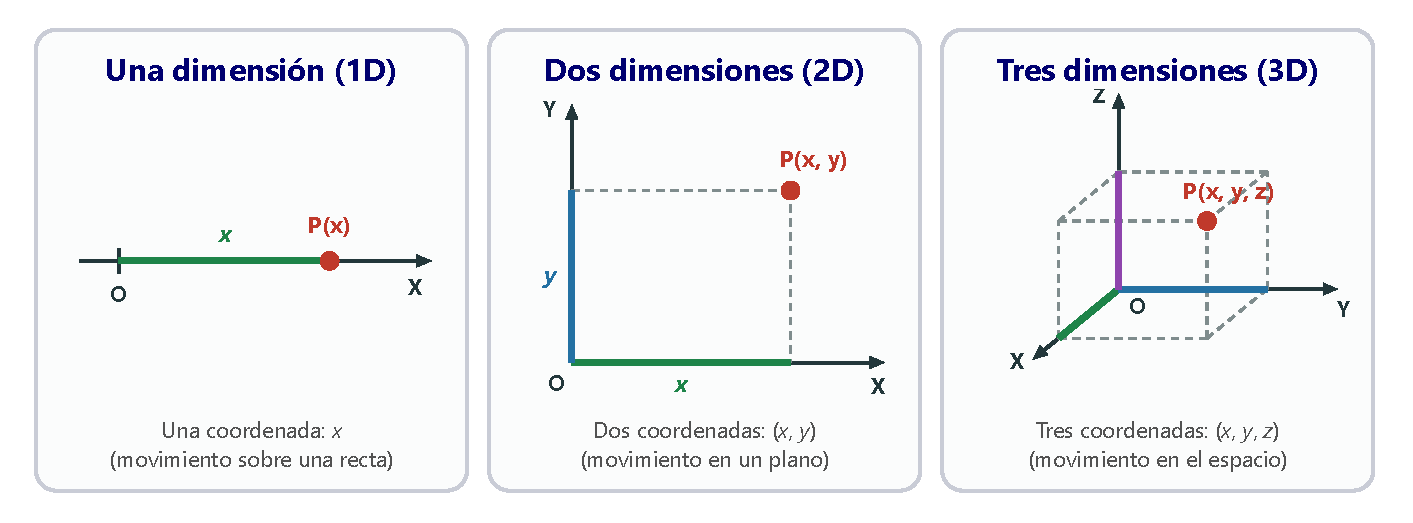
\includegraphics[width=0.95\textwidth]{images/UD8/sistemas_referencia}
    \caption{Según el movimiento, basta con una, dos o tres coordenadas para fijar la posición del móvil.}
    \label{fig:ud8-sr}
\end{figure}

Cualquier sistema de referencia permite describir el movimiento con igual validez, pero unos son más cómodos que otros: para un
coche en una carretera recta basta con un eje (1D); para un balón lanzado a canasta, con un plano (2D); para un avión, con tres
ejes (3D). Lo más práctico suele ser colocar el origen en la \textbf{posición del observador}. Un sistema de referencia siempre está
en reposo respecto a sí mismo, pero puede moverse respecto a otro: por eso se dice que el movimiento es \textbf{relativo}. En el
universo no existe ningún punto en reposo absoluto.

\begin{definition}[Sistemas inerciales y no inerciales]
    Un \textbf{sistema de referencia inercial} es aquel en el que un cuerpo sobre el que no actúa ninguna acción externa está en
    reposo o se mueve en línea recta con velocidad constante. Los sistemas inerciales están en reposo o se mueven con
    \textbf{velocidad constante} unos respecto a otros. Un sistema que tiene \textbf{aceleración} respecto a uno inercial es
    \textbf{no inercial}.
\end{definition}

Volvamos al telesilla. Si se detiene de golpe antes de llegar a la cumbre, la gente que espera en la cola (un S.R. inercial) ve que
tu cuerpo sigue moviéndose hacia delante un instante, porque nada lo ha frenado. Sin embargo, el asiento, que ha frenado
bruscamente, es un S.R. \textbf{no inercial}: desde él parece que algo te ha empujado hacia delante, aunque nadie lo ha hecho.

\begin{remark}
    \textbf{¿Es la Tierra un sistema inercial?} Estrictamente no: gira sobre sí misma y alrededor del Sol, así que tiene
    aceleración. Pero esas aceleraciones son tan pequeñas que, para los movimientos que estudiaremos este curso, la superficie
    terrestre es una \textbf{muy buena aproximación} de un sistema inercial.
\end{remark}

\begin{exercise}
    Indica si los siguientes sistemas se comportan como sistemas de referencia inerciales o no inerciales: a) un tren que arranca
    en la estación; b) un coche que circula a \qty{100}{\km\per\hour} constantes por una autovía recta; c) una niña, quieta en el
    suelo, que observa el vuelo de una cigüeña; d) un ascensor que arranca en la planta baja para subir al quinto piso; e) un
    autobús que toma una rotonda.
    \begin{solu}
        \textcolor{red}{Inerciales: b) y c)}, porque están en reposo o se mueven en línea recta con velocidad constante respecto
        al suelo. \textcolor{red}{No inerciales: a), d) y e)}: el tren y el ascensor aumentan su velocidad, y el autobús cambia la
        dirección de su velocidad; los tres tienen aceleración.
    \end{solu}
\end{exercise}

\subsection{Elementos del movimiento}

Los \textbf{elementos} que describen un movimiento son la \textbf{posición}, la \textbf{trayectoria}, el \textbf{vector
desplazamiento} y el \textbf{espacio recorrido}. Todos ellos dependen del sistema de referencia en que se midan.

\begin{definition}[Posición y trayectoria]
    La \textbf{posición} es el punto del espacio que ocupa el móvil en un instante dado. La \textbf{trayectoria} es el conjunto
    de puntos por los que pasa el móvil a lo largo del tiempo, es decir, la línea que une sus sucesivas posiciones.
\end{definition}

La trayectoria se obtiene registrando las posiciones \(s_0, s_1, s_2\ldots\) que ocupa el móvil en los instantes
\(t_0, t_1, t_2\ldots\) En la práctica, se suele tomar \(t_0 = 0\) al empezar a estudiar el movimiento.

\begin{figure}[H]
    \centering
    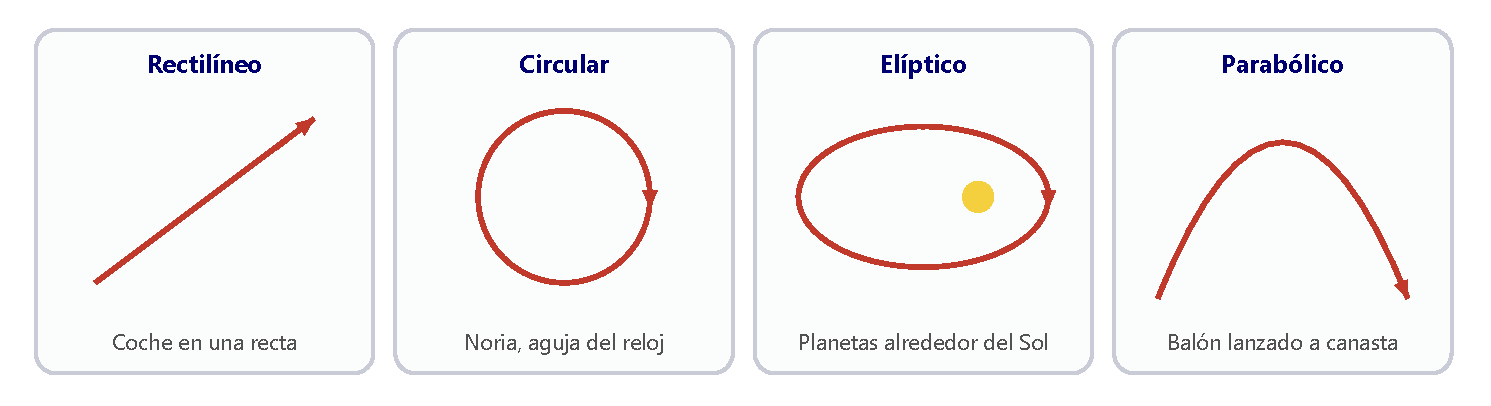
\includegraphics[width=0.85\textwidth]{images/UD8/tipos_trayectoria}
    \caption{Según la forma de la trayectoria, el movimiento es rectilíneo o curvilíneo (circular, elíptico, parabólico\ldots).}
    \label{fig:ud8-tipos}
\end{figure}

%========================================================================================
\section{Descripción del movimiento}\label{sec:ud8-descripcion}
%========================================================================================

\subsection{Vector posición y vector desplazamiento}

En un sistema de referencia de dos dimensiones, con vectores unitarios \(\ivec\) (eje X) y \(\jvec\) (eje Y), las dos magnitudes
básicas para describir el movimiento son vectoriales y se miden en metros:

\begin{definition}[Vector posición]
    El \textbf{vector posición} \(\vec r\) de un móvil es el vector que tiene su origen en el origen O del sistema de referencia
    y su extremo en el punto P\((x, y)\) que ocupa el móvil:
    \[ \vec r = \overrightarrow{OP} = x\,\ivec + y\,\jvec \qquad\qquad |\vec r| = \sqrt{x^2 + y^2} \]
    Su módulo es la distancia del móvil al origen.
\end{definition}

\begin{definition}[Vector desplazamiento]
    El \textbf{vector desplazamiento} \(\Delta\vec r\) es la diferencia entre los vectores posición final e inicial. Va de la
    posición inicial \(P_1(x_1, y_1)\) a la final \(P_2(x_2, y_2)\):
    \[ \Delta\vec r = \vec r_2 - \vec r_1 = (x_2 - x_1)\,\ivec + (y_2 - y_1)\,\jvec = \Delta x\,\ivec + \Delta y\,\jvec
    \qquad\qquad |\Delta\vec r| = \sqrt{(\Delta x)^2 + (\Delta y)^2} \]
\end{definition}

El módulo de un vector se calcula con el \textbf{teorema de Pitágoras} a partir de sus componentes. Si las posiciones inicial y
final coinciden, el desplazamiento es nulo, aunque el cuerpo se haya movido.

\begin{figure}[H]
    \centering
    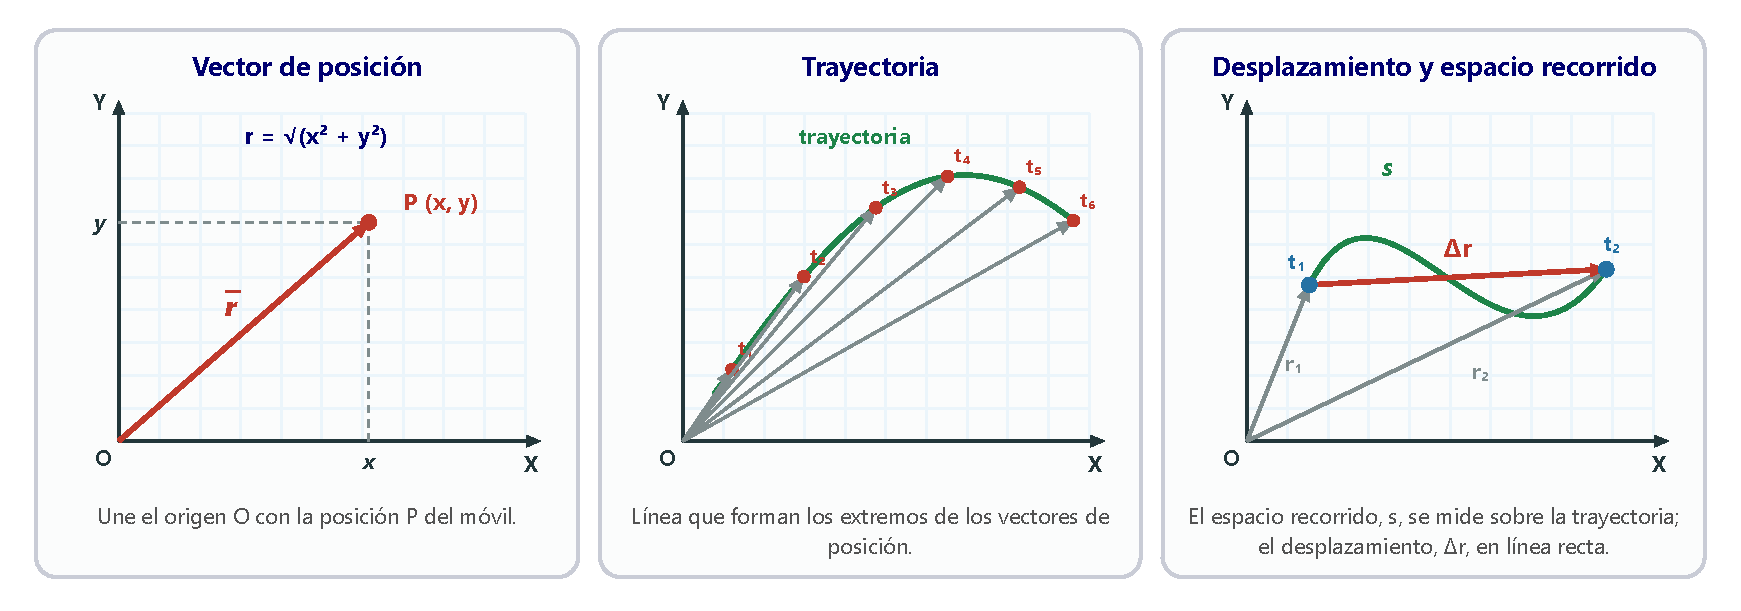
\includegraphics[width=\textwidth]{images/UD8/posicion_trayectoria}
    \caption{Vector posición, trayectoria y diferencia entre el desplazamiento y el espacio recorrido.}
    \label{fig:ud8-posicion}
\end{figure}

\begin{remark}
    \textbf{La posición depende del sistema de referencia.} Si el origen de un segundo sistema, \(O'\), tiene en el primero el
    vector posición \(\overrightarrow{OO'} = x_0\,\ivec + y_0\,\jvec\), la posición del punto P\((x, y)\) para el segundo
    observador es
    \[ \vec r\,' = \vec r - \overrightarrow{OO'} = (x - x_0)\,\ivec + (y - y_0)\,\jvec \]
\end{remark}

\begin{example}
    \textbf{Vectores posición.} Considera los puntos A\((0, 3)\), B\((-2, 0)\) y C\((4, 1)\), con las coordenadas en metros.
    a) Escribe sus vectores posición respecto al origen O\((0, 0)\) y calcula sus módulos. b) Escribe los vectores posición de
    A, B y C para un observador situado en \(O_1(1, 1)\).

    \textbf{Solución.} a) Cada vector posición tiene como componentes las coordenadas del punto:
    \[ \overrightarrow{OA} = 3\,\jvec~\unit{\m} \qquad \overrightarrow{OB} = -2\,\ivec~\unit{\m} \qquad \overrightarrow{OC} = (4\,\ivec + \jvec)~\unit{\m} \]
    \[ |\overrightarrow{OA}| = \qty{3}{\m} \qquad |\overrightarrow{OB}| = \qty{2}{\m} \qquad |\overrightarrow{OC}| = \sqrt{4^2 + 1^2} = \sqrt{17} = \qty{4.12}{\m} \]
    El módulo es la distancia de cada punto al origen: A está \qty{3}{\m} por encima de O; B, \qty{2}{\m} a su izquierda, y C, a
    \qty{4.12}{\m}.

    b) Restamos las coordenadas de \(O_1\):
    \[ \overrightarrow{O_1A} = (0 - 1)\,\ivec + (3 - 1)\,\jvec = (-\ivec + 2\,\jvec)~\unit{\m} \qquad
       \overrightarrow{O_1B} = (-3\,\ivec - \jvec)~\unit{\m} \qquad \overrightarrow{O_1C} = 3\,\ivec~\unit{\m} \]
\end{example}

\begin{example}
    \textbf{Dos caminos.} Una persona juega sobre un tablero de ajedrez gigante como si fuera una pieza; las coordenadas están en
    metros. Parte del punto A\((1, 1)\) y duda entre dos recorridos: ir al punto B\((3, 4)\) y después al C\((5, 7)\), o ir al
    D\((-2, 3)\) y después al E\((-5, 6)\). a) Calcula los vectores desplazamiento de cada tramo y el total de cada recorrido.
    b) ¿Al final de cuál de los dos recorridos queda más cerca de A?

    \textbf{Solución.} a) Primer recorrido:
    \[ \Delta\vec r_{AB} = (3 - 1)\,\ivec + (4 - 1)\,\jvec = (2\,\ivec + 3\,\jvec)~\unit{\m} \qquad
       \Delta\vec r_{BC} = (5 - 3)\,\ivec + (7 - 4)\,\jvec = (2\,\ivec + 3\,\jvec)~\unit{\m} \]
    \[ \Delta\vec r_1 = \Delta\vec r_{AB} + \Delta\vec r_{BC} = (4\,\ivec + 6\,\jvec)~\unit{\m} \]
    Segundo recorrido:
    \[ \Delta\vec r_{AD} = (-3\,\ivec + 2\,\jvec)~\unit{\m} \qquad \Delta\vec r_{DE} = (-3\,\ivec + 3\,\jvec)~\unit{\m} \qquad
       \Delta\vec r_2 = (-6\,\ivec + 5\,\jvec)~\unit{\m} \]
    Observa que el desplazamiento total es la suma de los desplazamientos parciales (y también \(\vec r_C - \vec r_A\)).

    b) \(|\Delta\vec r_1| = \sqrt{4^2 + 6^2} = \sqrt{52} = \qty{7.21}{\m}\) y \(|\Delta\vec r_2| = \sqrt{6^2 + 5^2} = \sqrt{61} =
    \qty{7.81}{\m}\). El punto C está más cerca de A que el punto E.
\end{example}

\begin{exercise}
    El vector posición de un móvil es \(\vec r_1 = (5\,\ivec - 12\,\jvec)~\unit{\m}\). Represéntalo y calcula a qué distancia
    está el móvil del origen.
    \begin{solu}
        \textcolor{blue}{Es una flecha desde O hasta el punto \((5, -12)\).} \(|\vec r_1| = \sqrt{5^2 + 12^2} = \textcolor{red}{\qty{13}{\m}}\).
    \end{solu}
\end{exercise}

\begin{exercise}
    El móvil del ejercicio anterior se desplaza hasta la posición \(\vec r_2 = (-8\,\ivec + 6\,\jvec)~\unit{\m}\). a) Represéntala
    en el mismo gráfico y calcula su módulo. b) Calcula el vector desplazamiento y su módulo, y dibújalo.
    \begin{solu}
        a) \(|\vec r_2| = \sqrt{64 + 36} = \textcolor{red}{\qty{10}{\m}}\). b) \(\Delta\vec r = \vec r_2 - \vec r_1 =
        \textcolor{red}{(-13\,\ivec + 18\,\jvec)~\unit{\m}}\), una flecha que va del extremo de \(\vec r_1\) al de \(\vec r_2\);
        \(|\Delta\vec r| = \sqrt{169 + 324} = \sqrt{493} = \textcolor{red}{\qty{22.2}{\m}}\).
    \end{solu}
\end{exercise}

\subsection{Trayectoria y espacio recorrido}

No hay que confundir dos conceptos que a menudo se mezclan:
\begin{itemize}
    \item la \textbf{trayectoria} es un concepto geométrico: la \textbf{línea} formada por los puntos que va ocupando el móvil;
    no tiene unidades;
    \item el \textbf{espacio recorrido}, \(e\) (o \(\Delta s\)), es la \textbf{distancia medida sobre la trayectoria}; es una
    magnitud \textbf{escalar} y se mide en metros.
\end{itemize}
Tampoco hay que confundir el espacio recorrido con el \textbf{módulo del desplazamiento}, que es la distancia \textbf{en línea
recta} entre la posición inicial y la final.

\begin{remark}
    \textbf{¿Una o dos dimensiones?} Los movimientos rectilíneos se suelen estudiar como unidimensionales, colocando el eje X sobre
    la propia trayectoria. Pero también se pueden describir en dos dimensiones si el origen del sistema de referencia está fuera
    de la recta; en ese caso, la posición tiene dos coordenadas que cambian a la vez.
\end{remark}

\begin{example}
    \textbf{Ida y vuelta.} Lucía sale de casa y camina en línea recta los \qty{300}{\m} que la separan de la biblioteca a
    \qty{1.5}{\m\per\s}. Estudia una hora y vuelve a casa por el mismo camino a \qty{2}{\m\per\s}. a) ¿Cuál ha sido su
    desplazamiento? b) ¿Qué espacio ha recorrido?

    \textbf{Solución.} a) Lucía vuelve al punto de partida: las posiciones inicial y final coinciden, así que
    \(\Delta\vec r = \vec 0\) y su desplazamiento es nulo. b) Ha recorrido \qty{300}{\m} a la ida y \qty{300}{\m} a la vuelta:
    \(e = \qty{600}{\m}\). (Las velocidades no influyen en ninguno de los dos resultados.)
\end{example}

\begin{exercise}
    Dos amigos suben a una atracción de feria en la que una plataforma circular de \qty{4}{\m} de radio da vueltas durante
    \qty{40}{\s}. Si en ese tiempo dan exactamente 6 vueltas, ¿cuál ha sido su desplazamiento y qué espacio han recorrido?
    \begin{solu}
        \textcolor{blue}{Acaban en el mismo punto en que empezaron.} \(\Delta\vec r = \vec 0\): \textcolor{red}{desplazamiento nulo};
        \(e = 6 \cdot 2\pi \cdot 4 = \textcolor{red}{\qty{151}{\m}}\).
    \end{solu}
\end{exercise}

\begin{exercise}
    En una excursión del instituto recorréis \qty{9}{\km} en dirección norte y después \qty{12}{\km} en dirección oeste. Calcula
    el módulo del desplazamiento y el espacio recorrido.
    \begin{solu}
        \textcolor{blue}{Tomando el eje X hacia el este y el Y hacia el norte: \(\Delta\vec r = (-12\,\ivec + 9\,\jvec)~\unit{\km}\).}
        \(|\Delta\vec r| = \sqrt{144 + 81} = \textcolor{red}{\qty{15}{\km}}\); \(e = 9 + 12 = \textcolor{red}{\qty{21}{\km}}\).
    \end{solu}
\end{exercise}

\subsection{El vector posición en función del tiempo}

Para describir completamente un movimiento hay que saber dónde está el móvil en \textbf{cada instante}. Para ello se expresan sus
coordenadas como funciones del tiempo:

\begin{definition}[Ecuación del movimiento]
    La \textbf{ecuación del movimiento} es la expresión del vector posición en función del tiempo:
    \[ \vec r(t) = x(t)\,\ivec + y(t)\,\jvec \]
    Dando valores a \(t\), se obtienen las coordenadas del móvil en ese instante. Las funciones \(x(t)\) e \(y(t)\) se llaman
    \textbf{ecuaciones paramétricas} del movimiento.
\end{definition}

El módulo \(|\vec r(t)| = \sqrt{x(t)^2 + y(t)^2}\) es la distancia del móvil al origen en el instante \(t\).

\subsection{El vector desplazamiento en función del tiempo}

Si \(\Delta t = t_2 - t_1\) es el intervalo de tiempo transcurrido entre dos instantes, el desplazamiento en ese intervalo es
\[ \Delta\vec r = \vec r(t_2) - \vec r(t_1) = (x_2 - x_1)\,\ivec + (y_2 - y_1)\,\jvec \qquad\qquad
   |\Delta\vec r| = \sqrt{(x_2 - x_1)^2 + (y_2 - y_1)^2} \]
En general, \(|\Delta\vec r|\) \textbf{no coincide con el espacio recorrido}, salvo en trayectorias rectilíneas sin cambio de
sentido. En una trayectoria cerrada, \(\Delta\vec r = \vec 0\), pero \(e \neq 0\).

\begin{example}
    \textbf{Movimiento en una dimensión.} La posición de un móvil sobre una recta viene dada por \(x(t) = 4t^2 - 2t\), en unidades
    del SI. Calcula: a) su posición en \(t = 0\), \(t = \qty{3}{\s}\) y \(t = \qty{8}{\s}\); b) su desplazamiento entre los
    segundos 3 y 8.

    \textbf{Solución.} a) Sustituimos cada valor de \(t\) en la ecuación:
    \[ x(0) = 0 \qquad x(3) = 4 \cdot 9 - 2 \cdot 3 = \qty{30}{\m} \qquad x(8) = 4 \cdot 64 - 2 \cdot 8 = \qty{240}{\m} \]
    b) \(\Delta x = x(8) - x(3) = 240 - 30 = \qty{210}{\m}\).
\end{example}

\begin{example}
    \textbf{Movimiento en el plano.} La posición de un móvil varía según \(\vec r(t) = (t^2 - 3t)\,\ivec + (4t + 2)\,\jvec\), en
    unidades del SI. a) Calcula su posición en \(t = 0\), \(t = \qty{2}{\s}\) y \(t = \qty{5}{\s}\). b) Determina el vector
    desplazamiento entre \(t = 0\) y \(t = \qty{2}{\s}\) y entre \(t = 0\) y \(t = \qty{5}{\s}\), y sus módulos.

    \textbf{Solución.} a) \(\vec r(0) = 2\,\jvec~\unit{\m}\); \(\vec r(2) = (4 - 6)\,\ivec + (8 + 2)\,\jvec = (-2\,\ivec + 10\,\jvec)~\unit{\m}\);
    \(\vec r(5) = (25 - 15)\,\ivec + (20 + 2)\,\jvec = (10\,\ivec + 22\,\jvec)~\unit{\m}\).

    b) \(\Delta\vec r_{0,2} = (-2\,\ivec + 10\,\jvec) - 2\,\jvec = (-2\,\ivec + 8\,\jvec)~\unit{\m}\), con módulo
    \(\sqrt{4 + 64} = \qty{8.25}{\m}\). \(\Delta\vec r_{0,5} = (10\,\ivec + 20\,\jvec)~\unit{\m}\), con módulo
    \(\sqrt{100 + 400} = \qty{22.4}{\m}\): el móvil está a \qty{8.25}{\m} de su punto de partida a los \qty{2}{\s}, y a
    \qty{22.4}{\m} a los \qty{5}{\s}.
\end{example}

\begin{example}
    \textbf{En una pista de skate.} Una rampa de skate tiene forma de media circunferencia de \qty{2.5}{\m} de radio. Calcula el
    desplazamiento y el espacio recorrido por un patinador que va: a) desde el borde de un lado (A) hasta el borde del otro lado
    (F); b) desde el borde A hasta el punto más bajo (M).

    \textbf{Solución.} El desplazamiento se mide en línea recta y el espacio, sobre el arco de circunferencia.
    a) A y F están en los extremos de un diámetro: \(|\Delta\vec r_{AF}| = 2r = \qty{5}{\m}\). El arco es media circunferencia:
    \(e_{AF} = \pi r = \qty{7.85}{\m}\).
    b) A y M forman un ángulo recto con el centro: \(|\Delta\vec r_{AM}| = \sqrt{r^2 + r^2} = r\sqrt 2 = \qty{3.54}{\m}\). El arco es
    un cuarto de circunferencia: \(e_{AM} = \dfrac{2\pi r}{4} = \qty{3.93}{\m}\). En las trayectorias curvas, el desplazamiento y
    el espacio recorrido no coinciden.
\end{example}

\begin{exercise}
    El vector posición de una cometa viene dado por \(\vec r(t) = 3t\,\ivec - (4t^2 + 2)\,\jvec\), en unidades del SI.
    a) Calcula su posición en \(t = 0\), \(t = \qty{4}{\s}\) y \(t = \qty{8}{\s}\). b) Determina el vector desplazamiento entre
    \(t = 0\) y \(t = \qty{4}{\s}\) y entre \(t = 0\) y \(t = \qty{8}{\s}\). c) Calcula sus módulos e interpreta el resultado.
    \begin{solu}
        a) \(\textcolor{red}{\vec r(0) = -2\,\jvec~\unit{\m}}\); \(\textcolor{red}{\vec r(4) = (12\,\ivec - 66\,\jvec)~\unit{\m}}\);
        \(\textcolor{red}{\vec r(8) = (24\,\ivec - 258\,\jvec)~\unit{\m}}\). b) \(\textcolor{red}{\Delta\vec r_{0,4} = (12\,\ivec - 64\,\jvec)~\unit{\m}}\);
        \(\textcolor{red}{\Delta\vec r_{0,8} = (24\,\ivec - 256\,\jvec)~\unit{\m}}\). c) \(\textcolor{red}{\qty{65.1}{\m}}\) y
        \(\textcolor{red}{\qty{257}{\m}}\): son las distancias en línea recta entre la posición inicial y las posiciones a los 4 y
        a los \qty{8}{\s}. (Con estos datos, la cometa estaría cayendo cada vez más deprisa: el eje Y apunta hacia arriba.)
    \end{solu}
\end{exercise}

\begin{exercise}
    La posición de un pez viene dada por \(\vec r(t) = 3t\,\ivec + (2t - 4)\,\jvec\), en unidades del SI. a) Calcula el
    desplazamiento del pez durante los seis primeros segundos. b) Calcula el desplazamiento durante los tres últimos segundos de
    ese intervalo e interpreta el resultado.
    \begin{solu}
        a) \(\vec r(0) = -4\,\jvec\); \(\vec r(6) = 18\,\ivec + 8\,\jvec\); \(\Delta\vec r = \textcolor{red}{(18\,\ivec + 12\,\jvec)~\unit{\m}}\).
        b) \(\vec r(3) = 9\,\ivec + 2\,\jvec\); \(\Delta\vec r = \textcolor{red}{(9\,\ivec + 6\,\jvec)~\unit{\m}}\): es la mitad
        del anterior en la mitad de tiempo, porque las coordenadas son funciones de primer grado de \(t\): el pez se mueve en
        línea recta y recorre lo mismo en cada segundo.
    \end{solu}
\end{exercise}

\subsection{La ecuación de la trayectoria}

Las ecuaciones paramétricas \(x(t)\) e \(y(t)\) están relacionadas a través del tiempo. Si eliminamos \(t\) entre ellas, obtenemos
una relación directa entre las coordenadas:

\begin{definition}[Ecuación de la trayectoria]
    La \textbf{ecuación de la trayectoria} se obtiene despejando \(t\) en una de las ecuaciones paramétricas y sustituyéndolo en la
    otra. Queda de la forma \(y = f(x)\) o \(x = f(y)\), y su gráfica es la forma de la trayectoria.
\end{definition}

Si la ecuación de la trayectoria es de primer grado, la trayectoria es una \textbf{recta}; si es de segundo grado, por ejemplo
\(y = a x^2 + b x + c\), es una \textbf{parábola}; y en general las funciones de grado superior dan trayectorias curvas.

\begin{example}
    \textbf{Trayectoria rectilínea.} Calcula la ecuación de la trayectoria de un móvil cuyo vector posición es
    \(\vec r(t) = (2t + 1)\,\ivec + (3t - 2)\,\jvec\), en metros, y represéntala.

    \textbf{Solución.} Separamos las coordenadas: \(x = 2t + 1\) e \(y = 3t - 2\). Despejamos \(t\) de la primera,
    \(t = \dfrac{x - 1}{2}\), y lo sustituimos en la segunda:
    \[ y = 3 \cdot \frac{x - 1}{2} - 2 \quad\Rightarrow\quad y = \frac{3x - 7}{2} \]
    Es una función de primer grado: la trayectoria es una \textbf{recta} (figura~\ref{fig:ud8-trayectorias}, izquierda).
\end{example}

\begin{example}
    \textbf{Trayectoria parabólica.} En los vuelos de entrenamiento en ingravidez, el avión describe una parábola. Determina la
    ecuación de la trayectoria de un avión de este tipo a partir de su vector posición, \(\vec r(t) = 8t\,\ivec + (2 - 5t^2)\,\jvec\)
    (en hectómetros y segundos), y represéntala.

    \textbf{Solución.} \(x = 8t\) e \(y = 2 - 5t^2\). Despejamos \(t = \dfrac{x}{8}\) y sustituimos:
    \[ y = 2 - 5 \left(\frac{x}{8}\right)^2 \quad\Rightarrow\quad y = 2 - \frac{5}{64}\,x^2 \]
    Es una función de segundo grado: la trayectoria es una \textbf{parábola} (figura~\ref{fig:ud8-trayectorias}, derecha). Solo
    tiene sentido físico para \(t \geq 0\), es decir, para \(x \geq 0\).
\end{example}

\begin{figure}[H]
    \centering
    \begin{tikzpicture}
        \begin{axis}[grafica, axis lines=middle, xlabel={\(x\) (m)}, ylabel={\(y\) (m)}, xmin=-1, xmax=7, ymin=-4, ymax=8,
            every axis x label/.style={at={(ticklabel* cs:1)}, anchor=west},
            every axis y label/.style={at={(ticklabel* cs:1)}, anchor=south}]
            \addplot[very thick, ocre, domain=1:7] {(3*x - 7)/2};
            \addplot[only marks, mark=*, mark size=1.8pt, ocre] coordinates {(1,-2) (3,1) (5,4) (7,7)};
            \node[font=\scriptsize, anchor=west] at (axis cs:3.1,0.6) {\(t = \qty{1}{\s}\)};
            \node[font=\scriptsize, anchor=west] at (axis cs:1.1,-2.6) {\(t = 0\)};
        \end{axis}
    \end{tikzpicture}\hspace{1cm}
    \begin{tikzpicture}
        \begin{axis}[grafica, axis lines=middle, xlabel={\(x\) (hm)}, ylabel={\(y\) (hm)}, xmin=-0.5, xmax=6, ymin=-1, ymax=2.6,
            every axis x label/.style={at={(ticklabel* cs:1)}, anchor=west},
            every axis y label/.style={at={(ticklabel* cs:1)}, anchor=south}]
            \addplot[very thick, ocre, domain=0:5.5] {2 - 5*x^2/64};
            \addplot[only marks, mark=*, mark size=1.8pt, ocre] coordinates {(0,2) (4,0.75)};
            \node[font=\scriptsize, anchor=south west] at (axis cs:0.1,2) {\(t = 0\)};
            \node[font=\scriptsize, anchor=south west] at (axis cs:4,0.8) {\(t = \qty{0.5}{\s}\)};
        \end{axis}
    \end{tikzpicture}
    \caption{Trayectorias de los ejemplos: una recta, \(y = (3x - 7)/2\), y una parábola, \(y = 2 - 5x^2/64\).}
    \label{fig:ud8-trayectorias}
\end{figure}

\begin{exercise}
    Un móvil se mueve según la ecuación \(\vec r(t) = (t + 5)\,\ivec + (3 - 6t)\,\jvec\), en metros. Determina analítica y
    gráficamente la ecuación de su trayectoria.
    \begin{solu}
        \textcolor{blue}{\(t = x - 5\); \(y = 3 - 6(x - 5)\).} \(\textcolor{red}{y = -6x + 33}\): una recta de pendiente \(-6\) que
        corta al eje Y en 33 (el móvil empieza en el punto \((5, 3)\)).
    \end{solu}
\end{exercise}

\begin{exercise}
    Calcula la ecuación de la trayectoria de un móvil cuyo vector posición es \(\vec r(t) = (3t - 2)\,\ivec + t^2\,\jvec\), en
    metros, y represéntala.
    \begin{solu}
        \textcolor{blue}{\(t = \dfrac{x + 2}{3}\).} \(\textcolor{red}{y = \dfrac{(x + 2)^2}{9}}\): una parábola con el vértice en
        \((-2, 0)\), que es la posición inicial.
    \end{solu}
\end{exercise}

\begin{exercise}
    El vector \(\vec r(t) = t^3\,\ivec + (5t - 4)\,\jvec\) (en metros) expresa la posición de una cometa durante su vuelo.
    Determina la ecuación de su trayectoria y descríbela.
    \begin{solu}
        \textcolor{blue}{Es más fácil despejar \(t\) de la coordenada \(y\): \(t = \dfrac{y + 4}{5}\).}
        \(\textcolor{red}{x = \left(\dfrac{y + 4}{5}\right)^3}\): es una función de tercer grado, así que la trayectoria es
        \textcolor{red}{curva}.
    \end{solu}
\end{exercise}

%========================================================================================
\section{La velocidad}\label{sec:ud8-velocidad}
%========================================================================================

En el día a día decimos que un vehículo es más rápido que otro si tarda menos en recorrer el mismo tramo. El concepto de velocidad
formaliza esta idea.

\begin{definition}[Velocidad]
    La \textbf{velocidad} es una magnitud física que informa del \textbf{cambio de posición} de un cuerpo y del \textbf{tiempo}
    empleado en él. Su unidad en el SI es el \unit{\m\per\s}.
\end{definition}

Según tengamos en cuenta o no la dirección y el sentido del movimiento, y según la duración del intervalo de tiempo, se definen
varios conceptos de velocidad.

\subsection{La velocidad media}

\begin{definition}[Velocidad media y celeridad media]
    La \textbf{velocidad media} \(\vec v_m\) es el cociente entre el vector desplazamiento y el tiempo empleado en él; es una
    magnitud \textbf{vectorial} con la misma dirección y sentido que \(\Delta\vec r\). La \textbf{celeridad} o \textbf{rapidez
    media} \(v_m\) es el cociente entre el espacio recorrido y el tiempo empleado; es una magnitud \textbf{escalar}:
    \[ \vec v_m = \frac{\Delta\vec r}{\Delta t} \qquad\qquad v_m = \frac{e}{\Delta t} \]
\end{definition}

La rapidez media no es, en general, el módulo de la velocidad media: solo coinciden en un movimiento rectilíneo sin cambios de
sentido. En una trayectoria cerrada, la velocidad media es nula, pero la rapidez media no. El inconveniente de los valores medios es
que no informan de lo que ocurre dentro del intervalo: la rapidez media de un esquiador en un slalom gigante puede ser de unos
\qty{70}{\km\per\hour}, pero no es la misma en la salida, al atravesar las puertas o al llegar a la meta.

\begin{example}
    \textbf{Al parque de atracciones.} Para ir a un parque de atracciones que está a \qty{21}{\km}, un grupo de amigos va en
    bicicleta y tarda \qty{45}{\minute}; otro va en coche y tarda \qty{20}{\minute}. Calcula la rapidez media de cada grupo en el SI.

    \textbf{Solución.} Bicicleta: \(v_{m1} = \dfrac{e}{\Delta t_1} = \dfrac{\qty{21000}{\m}}{45 \cdot \qty{60}{\s}} = \qty{7.78}{\m\per\s}\)
    (\qty{28}{\km\per\hour}). Coche: \(v_{m2} = \dfrac{\qty{21000}{\m}}{20 \cdot \qty{60}{\s}} = \qty{17.5}{\m\per\s}\)
    (\qty{63}{\km\per\hour}).
\end{example}

\begin{exercise}
    En una carrera solidaria, una corredora mantiene una rapidez media de \qty{12}{\km\per\hour} durante \qty{40}{\minute}.
    ¿Qué distancia recorre?
    \begin{solu}
        \(e = v_m\,\Delta t = 12 \cdot \dfrac{40}{60} = \qty{8}{\km} = \textcolor{red}{\qty{8e3}{\m}}\).
    \end{solu}
\end{exercise}

\begin{exercise}
    En un viaje de Sevilla a Madrid conducen dos personas por turnos. La primera recorre \qty{230}{\km} a una rapidez media de
    \qty{115}{\km\per\hour}, y la segunda, los \qty{300}{\km} restantes a \qty{100}{\km\per\hour}. ¿Cuánto dura el viaje? ¿Cuál es
    la rapidez media de todo el viaje?
    \begin{solu}
        \(t_1 = \dfrac{230}{115} = \qty{2}{\hour}\); \(t_2 = \dfrac{300}{100} = \qty{3}{\hour}\); \(\textcolor{red}{t = \qty{5}{\hour}}\).
        \(v_m = \dfrac{530}{5} = \textcolor{red}{\qty{106}{\km\per\hour}}\) (no es la media de las dos rapideces).
    \end{solu}
\end{exercise}

\subsection{La velocidad instantánea}

Cuanto más corto sea el intervalo de tiempo en que calculamos la velocidad media, más precisa será la información sobre el
movimiento. Así surge el concepto de \textbf{velocidad instantánea}, la velocidad que tiene el móvil en un instante concreto.

\begin{definition}[Velocidad instantánea]
    La \textbf{velocidad instantánea} es el límite de la velocidad media cuando el intervalo de tiempo tiende a cero:
    \[ \vec v = \lim_{\Delta t \to 0} \frac{\Delta\vec r}{\Delta t} = \lim_{\Delta t \to 0} \frac{\vec r(t + \Delta t) - \vec r(t)}{\Delta t} \]
\end{definition}

Cuando el intervalo es muy pequeño, el módulo del desplazamiento se confunde con el espacio recorrido, por lo que el módulo de la
velocidad instantánea es la \textbf{rapidez} o \textbf{celeridad instantánea}:
\[ |\vec v| = \lim_{\Delta t \to 0} \frac{|\Delta\vec r|}{\Delta t} = \lim_{\Delta t \to 0} \frac{e}{\Delta t} \]
Es lo que marca el \textbf{velocímetro} de un coche.

\begin{figure}[H]
    \centering
    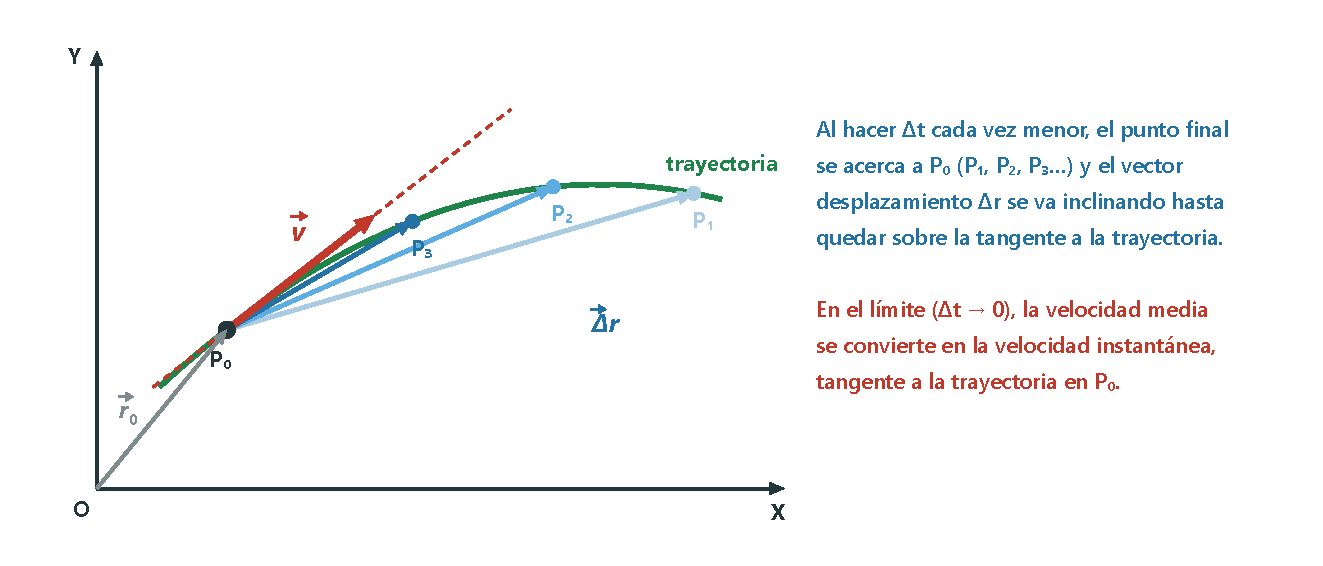
\includegraphics[width=0.85\textwidth]{images/UD8/velocidad_limite}
    \caption{Al reducir el intervalo de tiempo, el desplazamiento tiende a la dirección de la tangente.}
    \label{fig:ud8-limite}
\end{figure}

\begin{example}
    \textbf{Velocidad instantánea con la definición.} El vector posición de un móvil es \(\vec r(t) = 4t\,\ivec + (8 - t^2)\,\jvec\),
    en unidades del SI. a) Halla la velocidad instantánea aplicando la definición. b) Calcula la velocidad en \(t = \qty{1}{\s}\)
    y en \(t = \qty{3}{\s}\).

    \textbf{Solución.} a) Calculamos \(\vec r(t + \Delta t) = 4(t + \Delta t)\,\ivec + \big(8 - (t + \Delta t)^2\big)\,\jvec\) y
    restamos \(\vec r(t)\):
    \[ \vec r(t + \Delta t) - \vec r(t) = 4\,\Delta t\,\ivec + \big(-2t\,\Delta t - (\Delta t)^2\big)\,\jvec \]
    \[ \vec v = \lim_{\Delta t \to 0} \frac{4\,\Delta t\,\ivec + (-2t\,\Delta t - \Delta t^2)\,\jvec}{\Delta t}
       = \lim_{\Delta t \to 0} \big(4\,\ivec + (-2t - \Delta t)\,\jvec\big) = (4\,\ivec - 2t\,\jvec)~\unit{\m\per\s} \]
    b) \(\vec v(1) = (4\,\ivec - 2\,\jvec)~\unit{\m\per\s}\); \(\vec v(3) = (4\,\ivec - 6\,\jvec)~\unit{\m\per\s}\).
\end{example}

\subsubsection{Velocidad instantánea y derivada}

Calcular límites puede ser laborioso. Por suerte, el límite que define la velocidad es una operación matemática muy conocida: la
\textbf{derivada}.

\begin{definition}[Derivada]
    La \textbf{derivada} de una función \(f(t)\) respecto del tiempo indica \textbf{cómo cambia} la función al transcurrir el
    tiempo:
    \[ \frac{\dif f}{\dif t} = \lim_{\Delta t \to 0} \frac{f(t + \Delta t) - f(t)}{\Delta t} \]
    Por tanto, la \textbf{velocidad instantánea es la derivada del vector posición respecto del tiempo}:
    \[ \vec v = \frac{\dif\vec r}{\dif t} \]
\end{definition}

Las derivadas de las funciones más usadas están tabuladas, así que no hace falta calcular el límite cada vez:

\begin{table}[H]
    \centering
    \caption{Derivadas elementales (\(k\) y \(n\) son constantes; \(f\) y \(g\), funciones de \(t\))}
    \vspace{-5pt}
    \begin{tabular}{@{}lclc@{}}
        \toprule
        \textbf{Función} & \textbf{Derivada} & \textbf{Función} & \textbf{Derivada} \\
        \midrule
        \(k\) & \(0\) & \(\sen t\) & \(\cos t\) \\[3pt]
        \(t^n\) & \(n\,t^{n - 1}\) & \(\cos t\) & \(-\sen t\) \\[3pt]
        \(k \cdot f\) & \(k \cdot \dfrac{\dif f}{\dif t}\) & \(e^t\) & \(e^t\) \\[8pt]
        \(f \pm g\) & \(\dfrac{\dif f}{\dif t} \pm \dfrac{\dif g}{\dif t}\) & \(\ln t\) & \(\dfrac{1}{t}\) \\[8pt]
        \(f \cdot g\) & \(\dfrac{\dif f}{\dif t}\,g + f\,\dfrac{\dif g}{\dif t}\) & \(f^n\) & \(n\,f^{n - 1}\,\dfrac{\dif f}{\dif t}\) \\[8pt]
        \(\sen(\omega t)\) & \(\omega\cos(\omega t)\) & \(\sqrt f\) & \(\dfrac{1}{2\sqrt f}\,\dfrac{\dif f}{\dif t}\) \\
        \bottomrule
    \end{tabular}
    \label{tab:ud8-derivadas}
\end{table}

\begin{example}
    \textbf{Con la derivada.} La posición de un balón que rueda por el suelo es \(x(t) = 3 + 6t^2\), en unidades del SI.
    Calcula: a) la expresión de su velocidad; b) su velocidad en \(t = \qty{2}{\s}\) y en \(t = \qty{4}{\s}\).

    \textbf{Solución.} a) \(v(t) = \dfrac{\dif x}{\dif t} = 0 + 6 \cdot 2t = 12t~\unit{\m\per\s}\).
    b) \(v(2) = 12 \cdot 2 = \qty{24}{\m\per\s}\); \(v(4) = 12 \cdot 4 = \qty{48}{\m\per\s}\).
\end{example}

\subsubsection{El vector velocidad instantánea}

En un movimiento en el plano, \(\vec r = x(t)\,\ivec + y(t)\,\jvec\), la velocidad instantánea se obtiene derivando cada
componente por separado:
\[ \vec v = \frac{\dif x}{\dif t}\,\ivec + \frac{\dif y}{\dif t}\,\jvec = v_x\,\ivec + v_y\,\jvec \]
Las derivadas de las coordenadas son las componentes \(v_x\) y \(v_y\) de la velocidad. El vector velocidad instantánea tiene:
\begin{itemize}
    \item \textbf{módulo}: la rapidez del móvil, \(|\vec v| = \sqrt{v_x^2 + v_y^2}\);
    \item \textbf{dirección}: la de la recta \textbf{tangente} a la trayectoria en cada punto;
    \item \textbf{sentido}: el del movimiento.
\end{itemize}

\begin{figure}[H]
    \centering
    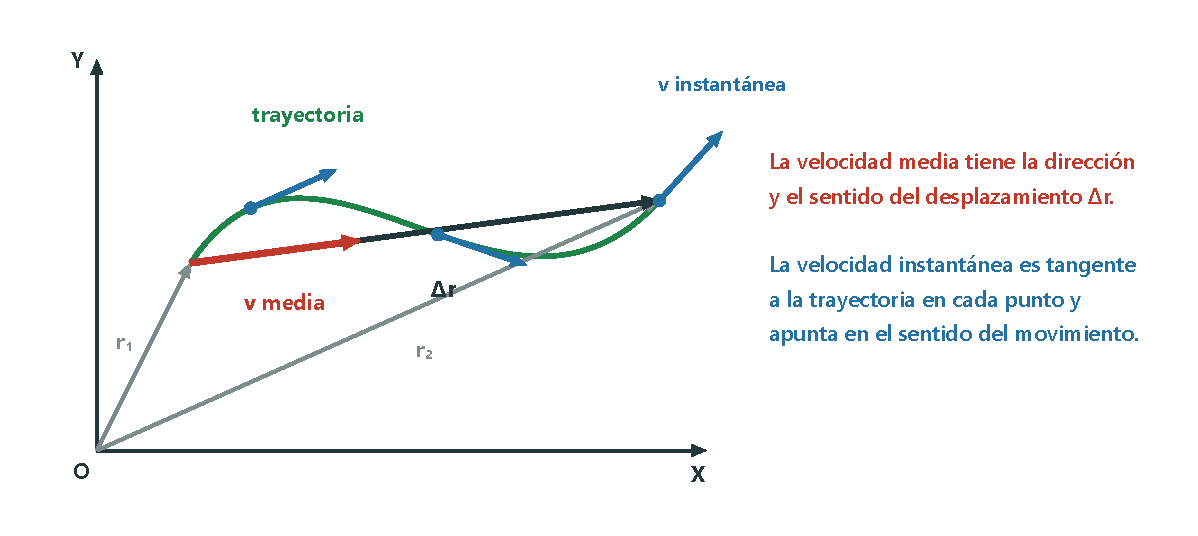
\includegraphics[width=0.8\textwidth]{images/UD8/velocidad_vector}
    \caption{La velocidad media tiene la dirección del desplazamiento; la instantánea es tangente a la trayectoria.}
    \label{fig:ud8-velocidad}
\end{figure}

\begin{example}
    \textbf{Vector velocidad y rapidez.} A partir de \(\vec r(t) = (0{,}5\,t^2 + 2)\,\ivec + (0{,}2\,t^2 - 1)\,\jvec\), en unidades
    del SI, determina: a) el vector velocidad instantánea; b) la velocidad en \(t = \qty{5}{\s}\); c) la rapidez en ese instante.

    \textbf{Solución.} a) Derivamos cada componente: \(\vec v(t) = 0{,}5 \cdot 2t\,\ivec + 0{,}2 \cdot 2t\,\jvec =
    (t\,\ivec + 0{,}4\,t\,\jvec)~\unit{\m\per\s}\). b) \(\vec v(5) = (5\,\ivec + 2\,\jvec)~\unit{\m\per\s}\).
    c) \(|\vec v(5)| = \sqrt{5^2 + 2^2} = \sqrt{29} = \qty{5.39}{\m\per\s}\).
\end{example}

\begin{exercise}
    El vector posición de una atracción de feria es \(\vec r(t) = (2t^2 + 1)\,\ivec + 3t\,\jvec\), en metros. Calcula: a) la
    expresión de la velocidad instantánea; b) el vector velocidad en \(t = \qty{2}{\s}\) y en \(t = \qty{4}{\s}\).
    \begin{solu}
        a) \(\textcolor{red}{\vec v = (4t\,\ivec + 3\,\jvec)~\unit{\m\per\s}}\). b) \(\textcolor{red}{\vec v(2) = (8\,\ivec + 3\,\jvec)~\unit{\m\per\s}}\);
        \(\textcolor{red}{\vec v(4) = (16\,\ivec + 3\,\jvec)~\unit{\m\per\s}}\).
    \end{solu}
\end{exercise}

\begin{exercise}
    Un coche teledirigido se mueve según \(\vec r(t) = (4t - t^2)\,\ivec + (t^2 - 2)\,\jvec\), en metros. Calcula: a) el módulo de
    la velocidad media en los cinco primeros segundos; b) la rapidez en \(t = \qty{2}{\s}\) y en \(t = \qty{5}{\s}\).
    \begin{solu}
        a) \textcolor{blue}{\(\vec r(0) = -2\,\jvec\); \(\vec r(5) = -5\,\ivec + 23\,\jvec\); \(\Delta\vec r = -5\,\ivec + 25\,\jvec\);
        \(\vec v_m = -\ivec + 5\,\jvec\).} \(|\vec v_m| = \sqrt{26} = \textcolor{red}{\qty{5.10}{\m\per\s}}\).
        b) \textcolor{blue}{\(\vec v = (4 - 2t)\,\ivec + 2t\,\jvec\).} \(\vec v(2) = 4\,\jvec\): \(\textcolor{red}{\qty{4}{\m\per\s}}\);
        \(\vec v(5) = -6\,\ivec + 10\,\jvec\): \(\sqrt{136} = \textcolor{red}{\qty{11.7}{\m\per\s}}\).
    \end{solu}
\end{exercise}

\subsection{La velocidad es relativa}

La posición y la trayectoria dependen del sistema de referencia, y también la velocidad: es una magnitud \textbf{relativa}.
Supongamos que dos observadores, O y A, miden la posición de un mismo cuerpo B. El observador O ve a A en la posición
\(\vec r_{AO}\) y a B en \(\vec r_{BO}\); el observador A ve a B en \(\vec r_{BA}\). Como se ve en la figura, \(\vec r_{BO} =
\vec r_{AO} + \vec r_{BA}\). Derivando respecto del tiempo:
\[ \vec v_{BO} = \vec v_{AO} + \vec v_{BA} \quad\Rightarrow\quad \boxed{\vec v_{BA} = \vec v_{BO} - \vec v_{AO}} \]
\(\vec v_{BA}\) es la \textbf{velocidad relativa} de B respecto a A. Esta relación entre las velocidades que miden dos observadores
inerciales es la \textbf{transformación de velocidades de Galileo}.

\begin{figure}[H]
    \centering
    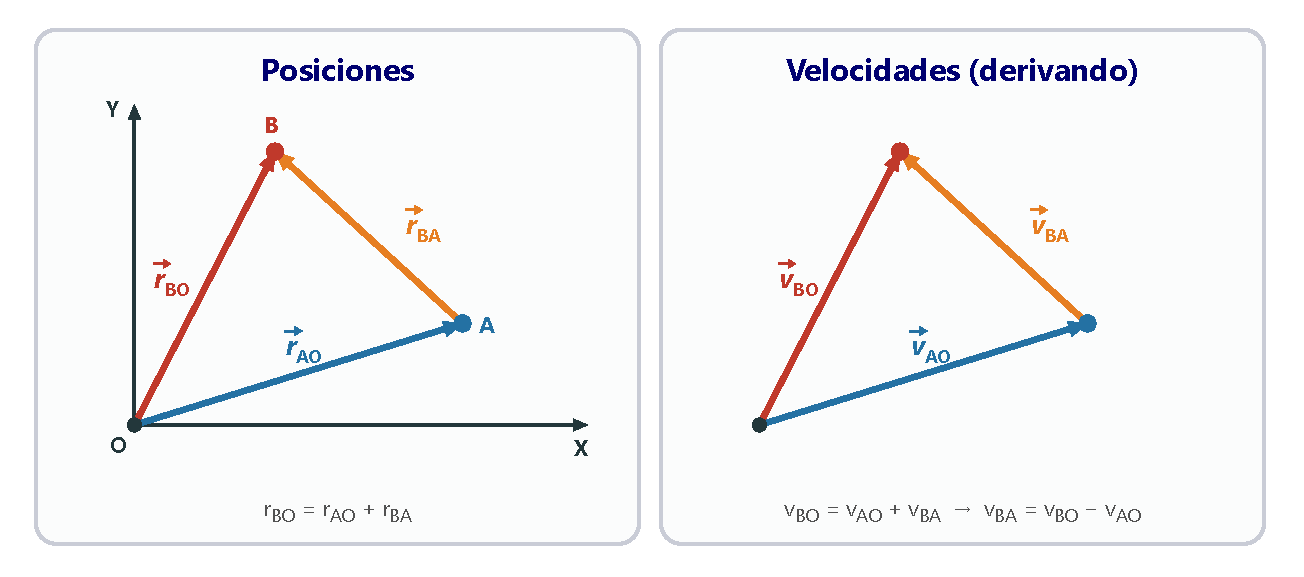
\includegraphics[width=0.75\textwidth]{images/UD8/velocidad_relativa}
    \caption{Posiciones y velocidades de un cuerpo B medidas por dos observadores, O y A.}
    \label{fig:ud8-relativa}
\end{figure}

\begin{remark}
    \textbf{Transformación de aceleraciones.} Si derivamos de nuevo, \(\vec a_{BO} = \vec a_{AO} + \vec a_{BA}\). Cuando los dos
    observadores son inerciales, A se mueve respecto a O con velocidad constante, así que \(\vec a_{AO} = \vec 0\) y queda
    \(\vec a_{BO} = \vec a_{BA}\): \textbf{todos los observadores inerciales miden la misma aceleración} para un cuerpo, aunque
    midan velocidades distintas.
\end{remark}

\begin{example}
    \textbf{En la carretera.} Por una carretera recta circulan un coche a \qty{90}{\km\per\hour} y una moto a \qty{110}{\km\per\hour}
    en el mismo sentido, y un camión a \qty{80}{\km\per\hour} en sentido contrario. Calcula la velocidad de la moto, del camión y
    del propio conductor del coche medidas desde el coche.

    \textbf{Solución.} Tomamos el eje X en el sentido del coche. Respecto al suelo: \(\vec v_C = 90\,\ivec\), \(\vec v_M = 110\,\ivec\)
    y \(\vec v_K = -80\,\ivec\) (en \unit{\km\per\hour}). El sistema de referencia es el coche:
    \[ \vec v_{M\text{-}C} = \vec v_M - \vec v_C = 110\,\ivec - 90\,\ivec = 20\,\ivec~\unit{\km\per\hour} \qquad
       \vec v_{K\text{-}C} = -80\,\ivec - 90\,\ivec = -170\,\ivec~\unit{\km\per\hour} \]
    El conductor se mueve con el coche: su velocidad relativa es nula. Por eso el camión parece «venir muy deprisa» y la moto
    nos adelanta despacio.
\end{example}

\begin{exercise}
    Un tren pasa por el andén a \qty{5}{\m\per\s}. Un viajero que va a perderlo corre tras él a \qty{7}{\m\per\s}, y dentro del
    tren el revisor camina hacia la cabina a \qty{1.5}{\m\per\s} respecto al tren. Determina: a) la velocidad del viajero
    respecto al tren; b) la velocidad del revisor respecto a la estación.
    \begin{solu}
        a) \(v_{VT} = 7 - 5 = \textcolor{red}{\qty{2}{\m\per\s}}\) en el sentido del tren: le alcanza. b) \(v_{RE} = 5 + \num{1.5} =
        \textcolor{red}{\qty{6.5}{\m\per\s}}\).
    \end{solu}
\end{exercise}

%========================================================================================
\section{La aceleración}\label{sec:ud8-aceleracion}
%========================================================================================

Si un cuerpo está sometido a interacciones, su velocidad puede cambiar en cualquiera de sus características: el
\textbf{módulo}, la \textbf{dirección} o el \textbf{sentido}. Un saltador de esquí aumenta su rapidez sin cambiar de dirección; un
\textit{snowboarder} cambia la dirección de su velocidad en cada giro; un yoyó cambia de sentido casi sin cambiar de rapidez.

\begin{definition}[Aceleración]
    La \textbf{aceleración} es una magnitud vectorial que mide los \textbf{cambios} que sufre el \textbf{vector velocidad} a lo
    largo del tiempo, ya sea en módulo, en dirección o en sentido. Su unidad en el SI es el \unit{\m\per\s\squared}.
\end{definition}

Siempre que la velocidad cambie, aunque sea mínimamente, la aceleración será distinta de cero. Según el tipo de cambio, hablaremos de
\textbf{aceleración tangencial} o de \textbf{aceleración normal} (o centrípeta), las componentes intrínsecas de la aceleración.

\subsection{La aceleración media}

\begin{definition}[Aceleración media]
    La \textbf{aceleración media} \(\vec a_m\) relaciona el cambio del vector velocidad con el intervalo de tiempo transcurrido:
    \[ \vec a_m = \frac{\Delta\vec v}{\Delta t} = \frac{\vec v_2 - \vec v_1}{t_2 - t_1} \]
    Tiene la misma dirección y sentido que el vector \(\Delta\vec v\).
\end{definition}

\begin{figure}[H]
    \centering
    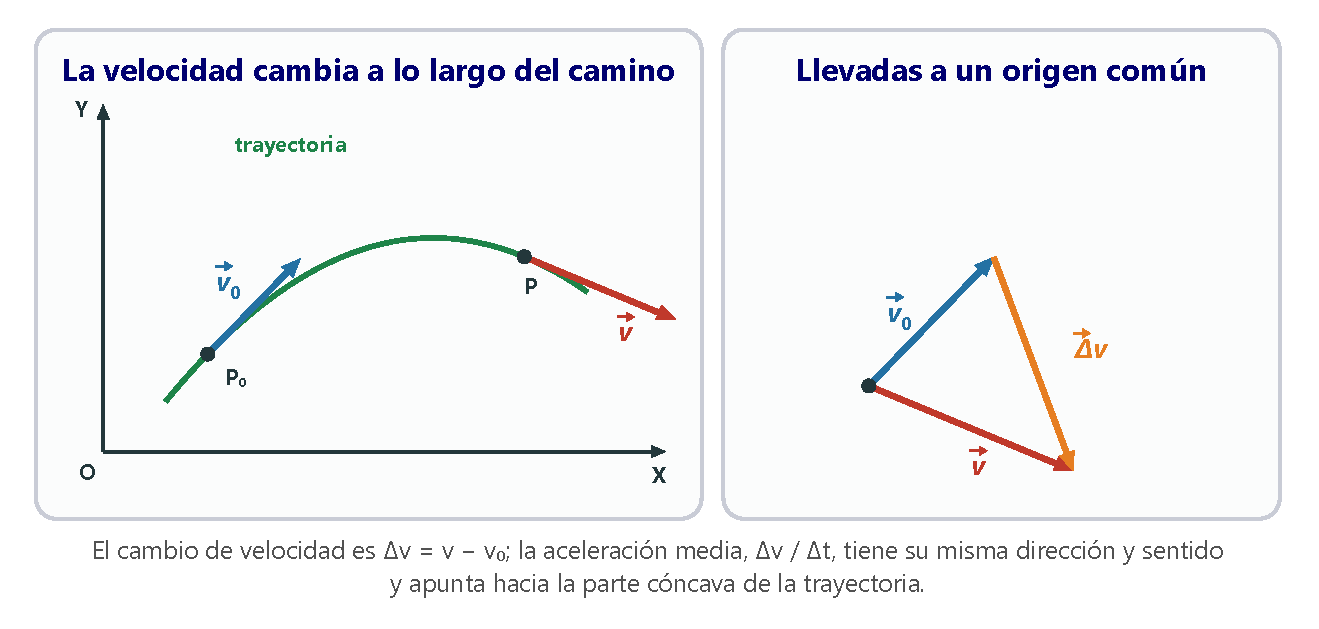
\includegraphics[width=0.85\textwidth]{images/UD8/aceleracion_media}
    \caption{En una trayectoria curva, \(\Delta\vec v\) (y la aceleración media) apunta hacia el interior de la curva.}
    \label{fig:ud8-am}
\end{figure}

\subsection{La aceleración instantánea}

\begin{definition}[Aceleración instantánea]
    La \textbf{aceleración instantánea} es el límite de la aceleración media cuando el intervalo de tiempo tiende a cero, es decir,
    la \textbf{derivada de la velocidad respecto del tiempo}:
    \[ \vec a = \lim_{\Delta t \to 0} \frac{\Delta\vec v}{\Delta t} = \frac{\dif\vec v}{\dif t} \]
\end{definition}

En el plano, si \(\vec v = v_x(t)\,\ivec + v_y(t)\,\jvec\), se deriva cada componente:
\[ \vec a = \frac{\dif v_x}{\dif t}\,\ivec + \frac{\dif v_y}{\dif t}\,\jvec = a_x\,\ivec + a_y\,\jvec \qquad\qquad |\vec a| = \sqrt{a_x^2 + a_y^2} \]
Como la velocidad es la derivada de la posición, la aceleración se obtiene derivando \textbf{dos veces} el vector posición:
\(\vec a = \dfrac{\dif^2\vec r}{\dif t^2}\).

La aceleración instantánea tiene la dirección y el sentido de \(\dif\vec v\), que en general \textbf{no es tangente} a la
trayectoria. En los movimientos rectilíneos tiene la dirección de la velocidad, aunque su sentido puede ser el mismo (el móvil
acelera) o el contrario (frena).

\begin{example}
    \textbf{Velocidad y aceleración en una dimensión.} Un objeto se mueve según \(x(t) = t^3 - 4t^2 + 2\), en unidades del SI.
    Determina: a) la expresión de la velocidad; b) la de la aceleración; c) la velocidad en \(t = \qty{4}{\s}\) y en
    \(t = \qty{6}{\s}\); d) la aceleración media entre esos instantes; e) la aceleración instantánea en \(t = \qty{4}{\s}\).

    \textbf{Solución.} a) \(v(t) = \dfrac{\dif x}{\dif t} = (3t^2 - 8t)~\unit{\m\per\s}\). b) \(a(t) = \dfrac{\dif v}{\dif t} =
    (6t - 8)~\unit{\m\per\s\squared}\). c) \(v(4) = 48 - 32 = \qty{16}{\m\per\s}\); \(v(6) = 108 - 48 = \qty{60}{\m\per\s}\).
    d) \(a_m = \dfrac{60 - 16}{6 - 4} = \qty{22}{\m\per\s\squared}\). e) \(a(4) = 24 - 8 = \qty{16}{\m\per\s\squared}\).
    La aceleración no es constante, así que la media y la instantánea son distintas.
\end{example}

\begin{example}
    \textbf{Aceleración media en el plano.} Un móvil tiene una velocidad \(\vec v(t) = -2t^2\,\ivec + 6\,\jvec\), en unidades del
    SI. Calcula la aceleración media en los cinco primeros segundos.

    \textbf{Solución.} \(\vec v(0) = 6\,\jvec~\unit{\m\per\s}\) y \(\vec v(5) = (-50\,\ivec + 6\,\jvec)~\unit{\m\per\s}\):
    \[ \vec a_m = \frac{\vec v(5) - \vec v(0)}{5 - 0} = \frac{-50\,\ivec}{5} = -10\,\ivec~\unit{\m\per\s\squared} \]
    La componente \(v_y\) no cambia, así que solo hay aceleración en el eje X.
\end{example}

\begin{example}
    \textbf{Aceleración con la definición de límite.} La velocidad de un móvil es \(\vec v(t) = (4t^2 - 2t)\,\ivec~\unit{\m\per\s}\).
    a) Calcula la aceleración instantánea con la definición de límite. b) Calcula la aceleración en \(t = \qty{1}{\s}\) y en
    \(t = \qty{5}{\s}\).

    \textbf{Solución.} a) \(\vec v(t + \Delta t) - \vec v(t) = \big[4(t + \Delta t)^2 - 2(t + \Delta t) - 4t^2 + 2t\big]\,\ivec =
    \big(8t\,\Delta t + 4\,\Delta t^2 - 2\,\Delta t\big)\,\ivec\), así que
    \[ \vec a = \lim_{\Delta t \to 0} \frac{(8t\,\Delta t + 4\,\Delta t^2 - 2\,\Delta t)\,\ivec}{\Delta t} =
       \lim_{\Delta t \to 0} (8t + 4\,\Delta t - 2)\,\ivec = (8t - 2)\,\ivec~\unit{\m\per\s\squared} \]
    b) \(\vec a(1) = 6\,\ivec~\unit{\m\per\s\squared}\); \(\vec a(5) = 38\,\ivec~\unit{\m\per\s\squared}\). (Derivando,
    \(\dfrac{\dif}{\dif t}(4t^2 - 2t) = 8t - 2\): el mismo resultado, mucho más rápido.)
\end{example}

\begin{exercise}
    Un patinador se desplaza según la función \(x(t) = 0{,}2\,t^3 + 2t - 5\), en metros. Determina: a) su velocidad; b) su
    aceleración; c) la velocidad en \(t = \qty{2}{\s}\) y en \(t = \qty{5}{\s}\); d) la aceleración media entre esos instantes;
    e) la aceleración en \(t = \qty{4}{\s}\).
    \begin{solu}
        a) \(\textcolor{red}{v = (0{,}6\,t^2 + 2)~\unit{\m\per\s}}\); b) \(\textcolor{red}{a = 1{,}2\,t~\unit{\m\per\s\squared}}\);
        c) \(\textcolor{red}{v(2) = \qty{4.4}{\m\per\s}}\) y \(\textcolor{red}{v(5) = \qty{17}{\m\per\s}}\);
        d) \(a_m = \dfrac{17 - \num{4.4}}{3} = \textcolor{red}{\qty{4.2}{\m\per\s\squared}}\); e) \(\textcolor{red}{a(4) = \qty{4.8}{\m\per\s\squared}}\).
    \end{solu}
\end{exercise}

\begin{exercise}
    Un coche entra en la autovía a \qty{36}{\km\per\hour} y, dos minutos después, circula a \qty{108}{\km\per\hour}. Calcula su
    aceleración media en unidades del SI.
    \begin{solu}
        \(a_m = \dfrac{30 - 10}{120} = \textcolor{red}{\qty{0.167}{\m\per\s\squared}}\).
    \end{solu}
\end{exercise}

\begin{exercise}
    Un objeto se mueve con una velocidad \(\vec v(t) = (2t^2 - 3t)\,\ivec + (t + 4)\,\jvec\), en \unit{\m\per\s}. a) Halla la
    aceleración instantánea con la definición de límite. Calcula: b) la velocidad al inicio y en \(t = \qty{10}{\s}\); c) la
    aceleración media en ese intervalo; d) la aceleración en \(t = \qty{5}{\s}\) y en \(t = \qty{10}{\s}\).
    \begin{solu}
        a) \textcolor{blue}{\(\Delta v_x = 4t\,\Delta t + 2\,\Delta t^2 - 3\,\Delta t\); \(\Delta v_y = \Delta t\).}
        \(\textcolor{red}{\vec a = (4t - 3)\,\ivec + \jvec~\unit{\m\per\s\squared}}\).
        b) \(\vec v(0) = \textcolor{red}{4\,\jvec~\unit{\m\per\s}}\) y \(\vec v(10) = \textcolor{red}{(170\,\ivec + 14\,\jvec)~\unit{\m\per\s}}\).
        c) \(\vec a_m = \Delta\vec v / \Delta t = \textcolor{red}{(17\,\ivec + \jvec)~\unit{\m\per\s\squared}}\).
        d) \(\vec a(5) = \textcolor{red}{(17\,\ivec + \jvec)~\unit{\m\per\s\squared}}\) y
        \(\vec a(10) = \textcolor{red}{(37\,\ivec + \jvec)~\unit{\m\per\s\squared}}\).
    \end{solu}
\end{exercise}

\subsection{Componentes intrínsecas de la aceleración}

Ya sabemos que hay aceleración no solo cuando cambia el valor de la velocidad, sino también cuando cambia su dirección, aunque la
rapidez sea constante. Para separar los dos efectos, se usa un sistema de referencia ligado a cada punto de la trayectoria, con un
eje \textbf{tangente} y otro \textbf{normal} (perpendicular) a ella. Sus vectores unitarios son \(\vec u_t\), tangente a la
trayectoria en el sentido del movimiento, y \(\vec u_n\), perpendicular a ella y dirigido hacia el centro de la curva.

\begin{definition}[Componentes intrínsecas]
    La aceleración se puede escribir como suma de dos componentes, llamadas \textbf{intrínsecas} porque están ligadas a cada punto
    de la trayectoria:
    \[ \vec a = \vec a_t + \vec a_n = a_t\,\vec u_t + a_n\,\vec u_n \qquad\qquad |\vec a| = \sqrt{a_t^2 + a_n^2} \]
\end{definition}

\begin{figure}[H]
    \centering
    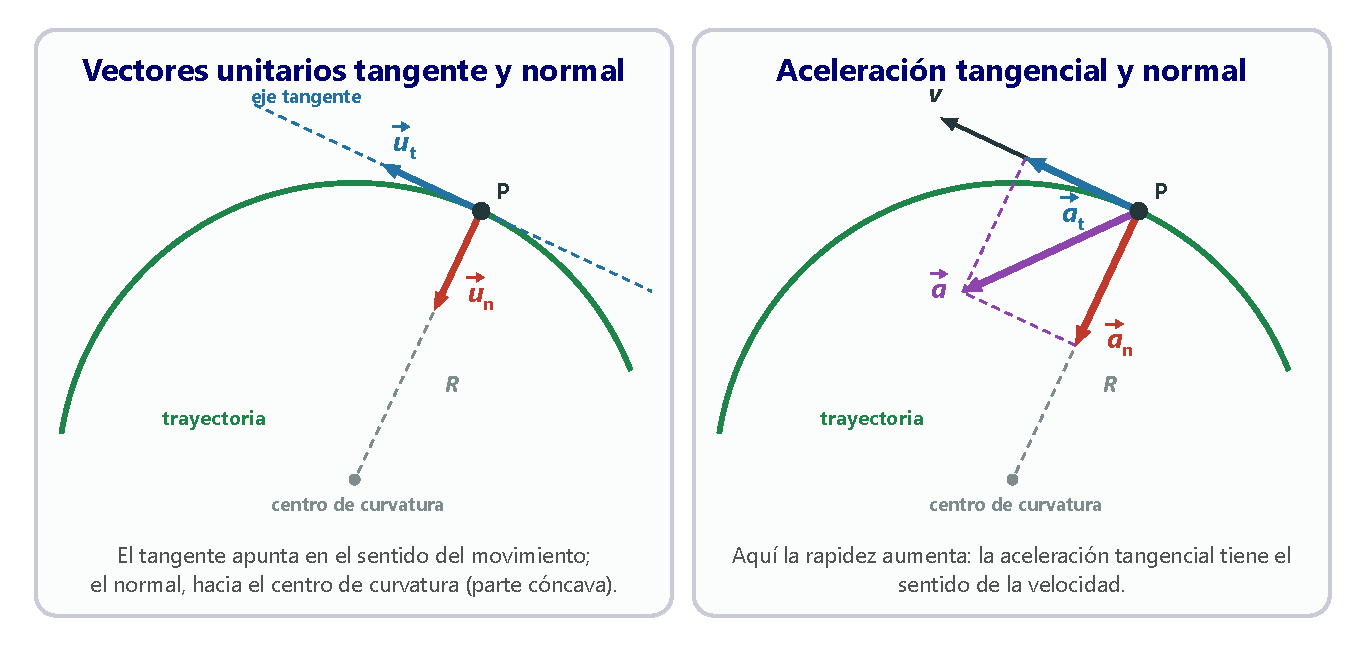
\includegraphics[width=0.9\textwidth]{images/UD8/componentes_intrinsecas}
    \caption{Sistema de referencia intrínseco y componentes tangencial y normal de la aceleración.}
    \label{fig:ud8-intrinsecas}
\end{figure}

\subsubsection{La aceleración tangencial}

Cuando la \textbf{rapidez} de un cuerpo cambia, aparece la \textbf{aceleración tangencial}, \textbf{paralela a la velocidad} en cada
punto. Su valor es la derivada del \textbf{módulo} de la velocidad:
\[ \vec a_t = \frac{\dif |\vec v|}{\dif t}\,\vec u_t \]
Si \(\vec a_t\) tiene el mismo sentido que \(\vec v\), la rapidez aumenta; si tiene sentido contrario, disminuye. Para derivar
el módulo de la velocidad, que suele ser una raíz, son útiles las reglas \(\dfrac{\dif(f^n)}{\dif t} = n\,f^{n - 1}\,\dfrac{\dif f}{\dif t}\)
y \(\dfrac{\dif\sqrt f}{\dif t} = \dfrac{1}{2\sqrt f}\,\dfrac{\dif f}{\dif t}\).

\subsubsection{La aceleración normal o centrípeta}

Cuando la \textbf{dirección} de la velocidad cambia, es decir, en las trayectorias curvas, aparece la \textbf{aceleración normal}
o \textbf{centrípeta}, \textbf{perpendicular a la trayectoria} y dirigida hacia el centro de la curva. Su valor depende de la
rapidez y del radio de curvatura \(R\) en ese punto:
\[ \vec a_n = \frac{v^2}{R}\,\vec u_n \]
En una trayectoria rectilínea, el radio es infinito y \(a_n = 0\). Un móvil puede tener aceleración tangencial, normal, ninguna de
las dos (movimiento rectilíneo y uniforme) o ambas a la vez.

\begin{table}[H]
    \centering
    \caption{Tipos de movimiento según las componentes intrínsecas de la aceleración}
    \vspace{-5pt}
    \begin{tabular}{@{}ccL{8cm}@{}}
        \toprule
        \(\boldsymbol{a_t}\) & \(\boldsymbol{a_n}\) & \textbf{Movimiento} \\
        \midrule
        \(0\) & \(0\) & Rectilíneo uniforme: la velocidad no cambia \\[3pt]
        \(\neq 0\) & \(0\) & Rectilíneo acelerado: cambia solo el módulo de la velocidad \\[3pt]
        \(0\) & \(\neq 0\) & Curvilíneo uniforme (por ejemplo, circular uniforme): cambia solo la dirección \\[3pt]
        \(\neq 0\) & \(\neq 0\) & Curvilíneo acelerado: cambian el módulo y la dirección \\
        \bottomrule
    \end{tabular}
    \label{tab:ud8-intrinsecas}
\end{table}

\begin{example}
    \textbf{Aceleración tangencial y normal a partir del vector posición.} Un cuerpo se mueve según
    \(\vec r(t) = (4t^2 - 1)\,\ivec + 2t^3\,\jvec\), en unidades del SI. Calcula: a) la aceleración tangencial en función del
    tiempo; b) las aceleraciones tangencial, total y normal en \(t = \qty{2}{\s}\); c) el radio de curvatura en ese instante.

    \textbf{Solución.} a) Derivamos para obtener la velocidad y su módulo (para \(t \geq 0\)):
    \[ \vec v = 8t\,\ivec + 6t^2\,\jvec \qquad\qquad |\vec v| = \sqrt{64t^2 + 36t^4} \]
    \[ a_t = \frac{\dif |\vec v|}{\dif t} = \frac{1}{2\sqrt{64t^2 + 36t^4}} \cdot (128t + 144t^3) = \frac{64t + 72t^3}{\sqrt{64t^2 + 36t^4}}~\unit{\m\per\s\squared} \]
    b) \(a_t(2) = \dfrac{128 + 576}{\sqrt{256 + 576}} = \dfrac{704}{\num{28.84}} = \qty{24.4}{\m\per\s\squared}\).
    La aceleración total es \(\vec a = \dfrac{\dif\vec v}{\dif t} = 8\,\ivec + 12t\,\jvec\); en \(t = \qty{2}{\s}\),
    \(\vec a = 8\,\ivec + 24\,\jvec\) y \(|\vec a| = \sqrt{640} = \qty{25.3}{\m\per\s\squared}\). Despejando de
    \(a^2 = a_t^2 + a_n^2\):
    \[ a_n = \sqrt{a^2 - a_t^2} = \sqrt{640 - \num{24.4}^2} = \qty{6.66}{\m\per\s\squared} \]
    c) \(R = \dfrac{v^2}{a_n} = \dfrac{832}{\num{6.66}} = \qty{125}{\m}\).
\end{example}

\begin{example}
    \textbf{En una curva.} Un coche entra en una curva de \qty{20}{\m} de radio a \qty{15}{\m\per\s} y sale de ella a
    \qty{25}{\m\per\s}; tarda \qty{4}{\s} en recorrerla. Calcula: a) la aceleración tangencial, suponiendo que es constante; b) la
    aceleración normal a la entrada y a la salida de la curva; c) el módulo de la aceleración total a la entrada.

    \textbf{Solución.} a) \(a_t = \dfrac{\Delta v}{\Delta t} = \dfrac{25 - 15}{4} = \qty{2.5}{\m\per\s\squared}\).
    b) \(a_{n1} = \dfrac{v_1^2}{R} = \dfrac{15^2}{20} = \qty{11.25}{\m\per\s\squared}\); \(a_{n2} = \dfrac{25^2}{20} =
    \qty{31.25}{\m\per\s\squared}\). c) \(a = \sqrt{a_t^2 + a_n^2} = \sqrt{\num{2.5}^2 + \num{11.25}^2} = \qty{11.5}{\m\per\s\squared}\).
\end{example}

\begin{exercise}
    Calcula la aceleración centrípeta de un niño montado en un tiovivo de \qty{4}{\m} de radio que gira con una rapidez constante
    de \qty{3}{\m\per\s}. ¿Tiene aceleración tangencial?
    \begin{solu}
        \(a_n = \dfrac{3^2}{4} = \textcolor{red}{\qty{2.25}{\m\per\s\squared}}\). \textcolor{red}{No tiene aceleración tangencial},
        porque su rapidez no cambia.
    \end{solu}
\end{exercise}

\begin{exercise}
    Un móvil entra en una curva de \qty{8}{\m} de radio a \qty{4}{\m\per\s} con una aceleración tangencial constante de
    \qty{2}{\m\per\s\squared}. Si tarda \qty{3}{\s} en recorrer la curva, calcula: a) la velocidad y la aceleración normal a la
    salida de la curva; b) la aceleración total en ese momento.
    \begin{solu}
        a) \(v = 4 + 2 \cdot 3 = \textcolor{red}{\qty{10}{\m\per\s}}\); \(a_n = \dfrac{100}{8} = \textcolor{red}{\qty{12.5}{\m\per\s\squared}}\).
        b) \(a = \sqrt{2^2 + \num{12.5}^2} = \textcolor{red}{\qty{12.7}{\m\per\s\squared}}\).
    \end{solu}
\end{exercise}

\begin{exercise}
    Un avión de exhibición describe círculos de \qty{50}{\m} de radio con una rapidez \(v(t) = (2t^2 + 10)~\unit{\m\per\s}\).
    Determina: a) las expresiones de la aceleración tangencial y de la normal, y sus valores en \(t = \qty{3}{\s}\); b) el módulo de
    la aceleración en \(t = \qty{3}{\s}\) y en \(t = \qty{5}{\s}\).
    \begin{solu}
        a) \(\textcolor{red}{a_t = 4t~\unit{\m\per\s\squared}}\); \(\textcolor{red}{a_n = \dfrac{(2t^2 + 10)^2}{50}~\unit{\m\per\s\squared}}\).
        En \(t = \qty{3}{\s}\): \(v = \qty{28}{\m\per\s}\), \(\textcolor{red}{a_t = \qty{12}{\m\per\s\squared}}\) y
        \(\textcolor{red}{a_n = \qty{15.7}{\m\per\s\squared}}\). b) \(a(3) = \sqrt{12^2 + \num{15.68}^2} = \textcolor{red}{\qty{19.7}{\m\per\s\squared}}\);
        en \(t = \qty{5}{\s}\): \(v = \qty{60}{\m\per\s}\), \(a_t = 20\), \(a_n = 72\) y \(a = \textcolor{red}{\qty{74.7}{\m\per\s\squared}}\).
    \end{solu}
\end{exercise}

%========================================================================================
\section{Física en la vida: ¿competiciones más justas gracias a la tecnología?}\label{sec:ud8-cronometraje}
%========================================================================================

En las grandes competiciones de atletismo o de natación, las medallas se deciden a veces por centésimas o incluso milésimas de
segundo. ¿Cómo se miden tiempos tan pequeños?

Durante mucho tiempo el cronometraje fue \textbf{manual}: una persona ponía en marcha el cronómetro al oír el disparo de salida y lo
paraba al ver llegar al deportista, así que el tiempo dependía de sus reflejos. En los Juegos Olímpicos de Los Ángeles de 1932 se
usaron ya decenas de cronógrafos de precisión que medían décimas de segundo. Después llegaron las \textbf{células fotoeléctricas},
que detectan el paso del atleta por la meta, y la \textbf{foto finish}, una cámara que fotografía continuamente la línea de llegada
y permite ordenar a los corredores aunque lleguen casi a la vez. En natación se introdujeron \textbf{placas de contacto} que el
nadador pulsa con la mano al tocar la pared, y en la salida, tacos con sensores que detectan las \textbf{salidas nulas} (un atleta
que reacciona en menos de una décima de segundo después del disparo se considera que ha salido antes de tiempo, porque el ser humano
no puede reaccionar tan deprisa).

Hoy los tiempos se miden con una precisión de milésimas, se transmiten al instante y se completan con sensores que registran la
posición y la velocidad de cada deportista en tiempo real. Pero también surgen preguntas: en los Juegos de Pekín de 2008, Michael
Phelps ganó los 100 metros mariposa por \textbf{una centésima}. ¿Es justa una diferencia tan pequeña? ¿Y si las calles de la
piscina no midieran exactamente lo mismo?

\begin{table}[H]
    \centering
    \caption{Final masculina de 100 metros lisos de los Juegos Olímpicos de Tokio (2021)}
    \vspace{-5pt}
    \begin{tabular}{@{}lcccc@{}}
        \toprule
        \textbf{Atleta} & Jacobs & Kerley & De Grasse & Simbine \\
        \midrule
        \textbf{Tiempo (s)} & \num{9.80} & \num{9.84} & \num{9.89} & \num{9.93} \\
        \bottomrule
    \end{tabular}
    \label{tab:ud8-tokio}
\end{table}

\begin{exercise}
    Con los datos de la tabla~\ref{tab:ud8-tokio}: a) calcula la rapidez media de cada atleta; b) suponiendo que Kerley corriera
    siempre a su rapidez media, ¿a qué distancia de la meta estaba cuando Jacobs la cruzó?; c) ¿qué distancia recorre en una
    centésima de segundo un atleta a \qty{10}{\m\per\s}?; d) en la final de Pekín, Phelps hizo \qty{50.58}{\s} en los
    \qty{100}{\m}. ¿Por cuántos centímetros ganó? e) Debatid: ¿ha hecho la tecnología más justas las competiciones? ¿Cómo ha
    cambiado la participación de las mujeres en los Juegos Olímpicos en los últimos cien años?
    \begin{solu}
        a) \(v_m = 100/t\): \textcolor{red}{Jacobs \qty{10.20}{\m\per\s}; Kerley \qty{10.16}{\m\per\s}; De Grasse
        \qty{10.11}{\m\per\s}; Simbine \qty{10.07}{\m\per\s}}. b) En \qty{9.80}{\s}, Kerley recorre
        \(\num{10.163} \cdot \num{9.80} = \qty{99.59}{\m}\): estaba a \(\textcolor{red}{\approx \qty{41}{\cm}}\) de la meta.
        c) \(10 \cdot \num{0.01} = \textcolor{red}{\qty{0.1}{\m} = \qty{10}{\cm}}\). d) \(v_m = \dfrac{100}{\num{50.58}} =
        \qty{1.98}{\m\per\s}\); en \qty{0.01}{\s} recorre \(\textcolor{red}{\approx \qty{2}{\cm}}\). e) \textcolor{red}{Respuesta
        abierta}. En 1900 participaron 22 mujeres entre casi mil deportistas; en Tokio, casi la mitad fueron mujeres.
    \end{solu}
\end{exercise}

%========================================================================================
\section{Prácticas}\label{sec:ud8-practicas}
%========================================================================================

\subsection{Un aerodeslizador casero}

\noindent\begin{minipage}[t]{0.48\textwidth}
    \textbf{Objetivo}
    \begin{itemize}
        \item Construir un aerodeslizador con materiales sencillos, describir su movimiento (trayectoria, desplazamiento y espacio
        recorrido) y medir su rapidez media.
    \end{itemize}
\end{minipage}\hfill
\begin{minipage}[t]{0.48\textwidth}
    \textbf{Material}
    \begin{itemize}
        \item Un CD o DVD viejo, un trozo de cartón, una botella de plástico con tapón de rosca, un globo mediano, pegamento
        termofusible, un punzón, cinta métrica y cronómetro (o el móvil).
    \end{itemize}
\end{minipage}

\medskip
Un \textbf{aerodeslizador} se desplaza sobre un colchón de aire que él mismo expulsa hacia el suelo. Como apenas toca la superficie,
el rozamiento es muy pequeño y se mueve con mucha facilidad. Los de verdad pueden superar los \qty{100}{\km\per\hour} y se usan como
vehículos de rescate, de transporte entre islas o militares.

\begin{figure}[H]
    \centering
    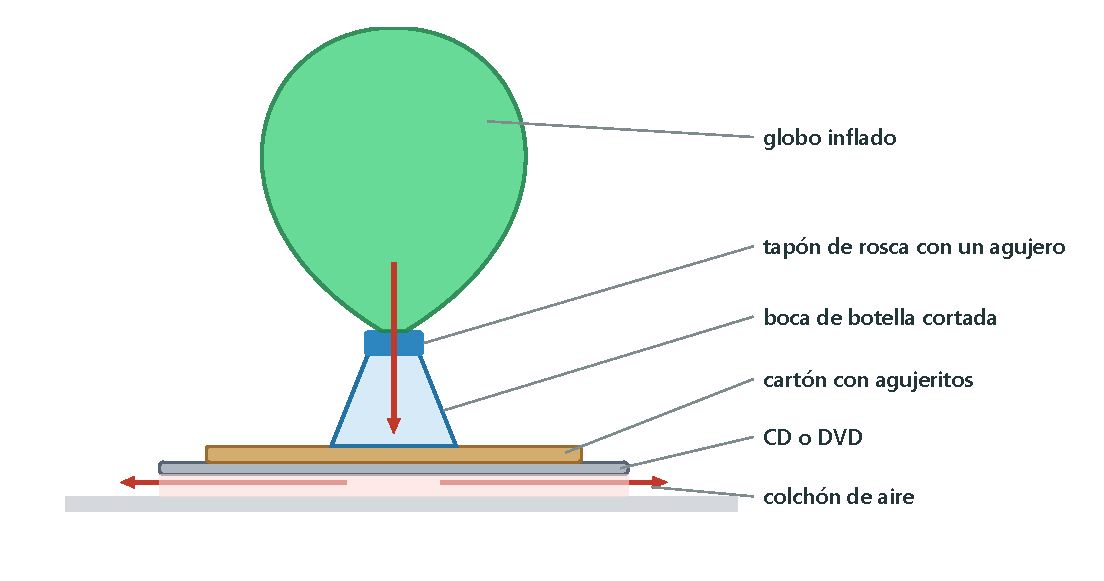
\includegraphics[width=0.55\textwidth]{images/UD8/aerodeslizador}
    \caption{Esquema del aerodeslizador casero: el aire del globo sale por debajo del CD y lo hace flotar.}
    \label{fig:ud8-aerodeslizador}
\end{figure}

\textbf{Procedimiento}
\begin{enumerate}[label=\numberballgreen]
    \item Recorta un círculo de cartón del tamaño del CD (sin el agujero central) y haz con el punzón varios agujeritos en su zona
    central.
    \item Corta la parte superior de la botella, en forma de cono, y haz un agujero de unos \qty{3}{\mm} en el tapón.
    \item Pega el cono de la botella sobre el cartón, tapando los agujeritos, y el cartón sobre el CD, de modo que el aire solo
    pueda salir por el agujero central del disco.
    \item Infla el globo, retuerce la boquilla para que no se escape el aire y encájalo en el tapón.
    \item Coloca el aerodeslizador en una mesa lisa, suelta el globo y dale un pequeño impulso.
    \item Diseña un circuito y mide las distancias recorridas y los tiempos que tarda en recorrerlas. Repite cada medida cinco veces.
    \item Si puedes, graba el movimiento con el móvil y analízalo con un programa de análisis de vídeo, como Tracker.
\end{enumerate}

\begin{exercise}
    a) ¿Por qué el aerodeslizador se mueve con tanta facilidad? ¿Qué ocurre cuando se acaba el aire del globo? b) Describe su
    trayectoria y dibuja el desplazamiento y el espacio recorrido en un recorrido de ida y vuelta. c) En cinco medidas, el
    aerodeslizador tarda 2,3; 2,5; 2,4; 2,6 y \qty{2.2}{\s} en recorrer \qty{1.20}{\m} en línea recta. Calcula el tiempo medio y su
    rapidez media. d) Organiza en una tabla los resultados de tus propias medidas.
    \begin{solu}
        a) \textcolor{red}{Porque el colchón de aire evita casi todo el rozamiento con la mesa}; cuando se acaba el aire, el CD
        toca la mesa y se frena enseguida. b) \textcolor{red}{Respuesta abierta}: en un recorrido de ida y vuelta el desplazamiento
        es nulo y el espacio recorrido es el doble de la distancia. c) \(\bar t = \dfrac{\num{12.0}}{5} = \textcolor{red}{\qty{2.4}{\s}}\);
        \(v_m = \dfrac{\num{1.20}}{\num{2.4}} = \textcolor{red}{\qty{0.50}{\m\per\s}}\). d) \textcolor{red}{Respuesta abierta}.
    \end{solu}
\end{exercise}

\subsection{De la velocidad media a la instantánea con un vídeo}

\noindent\begin{minipage}[t]{0.48\textwidth}
    \textbf{Objetivo}
    \begin{itemize}
        \item Obtener la posición de un móvil en función del tiempo a partir de un vídeo y calcular su velocidad y su aceleración.
    \end{itemize}
\end{minipage}\hfill
\begin{minipage}[t]{0.48\textwidth}
    \textbf{Material}
    \begin{itemize}
        \item Una tabla larga o un carril inclinado, una canica o un coche de juguete, una cinta métrica y un móvil con cámara;
        programa Tracker (gratuito) o una hoja de cálculo.
    \end{itemize}
\end{minipage}

\textbf{Procedimiento}
\begin{enumerate}[label=\numberballgreen]
    \item Inclina ligeramente la tabla y pega a su lado la cinta métrica, que servirá de escala.
    \item Graba con el móvil, fijo y perpendicular a la tabla, cómo baja la canica soltada desde el reposo.
    \item Con Tracker, marca la posición de la canica fotograma a fotograma (o pausa el vídeo cada pocos fotogramas y lee la cinta).
    \item Anota en una tabla las parejas (\(t\), \(x\)) y representa \(x\) frente a \(t\).
\end{enumerate}

\begin{table}[H]
    \centering
    \caption{Posición de una canica que baja por un carril inclinado, obtenida de un vídeo}
    \vspace{-5pt}
    \begin{tabular}{@{}lcccccc@{}}
        \toprule
        \(\boldsymbol{t}\) \textbf{(s)} & 0 & \num{0.2} & \num{0.4} & \num{0.6} & \num{0.8} & \num{1.0} \\
        \midrule
        \(\boldsymbol{x}\) \textbf{(cm)} & 0 & 4 & 16 & 36 & 64 & 100 \\
        \bottomrule
    \end{tabular}
    \label{tab:ud8-canica}
\end{table}

\begin{exercise}
    Con los datos de la tabla~\ref{tab:ud8-canica}: a) calcula la velocidad media en cada intervalo de \qty{0.2}{\s}; b) asigna
    cada velocidad media al instante central de su intervalo y representa \(v\) frente a \(t\). ¿Qué forma tiene la gráfica?
    c) Comprueba que \(x(t) = 100\,t^2\) (en cm y s) y obtén, derivando, \(v(t)\) y \(a(t)\). d) ¿Por qué la velocidad media en un
    intervalo coincide aquí con la instantánea en su punto medio?
    \begin{solu}
        a) \(\textcolor{red}{20, 60, 100, 140~\text{y}~\qty{180}{\cm\per\s}}\). b) En \(t = \numlist{0.1;0.3;0.5;0.7;0.9}~\unit{\s}\):
        los puntos están \textcolor{red}{alineados en una recta que pasa por el origen}, \(v = 200\,t\). c) \(x(0{,}4) = 100 \cdot
        \num{0.16} = 16\) \ldots\ se cumple; \(\textcolor{red}{v = 200\,t~\unit{\cm\per\s}}\) y \(\textcolor{red}{a = \qty{200}{\cm\per\s\squared}
        = \qty{2}{\m\per\s\squared}}\), constante. d) \textcolor{red}{Porque la velocidad cambia de forma lineal con el tiempo}
        (aceleración constante): su valor medio en un intervalo es el valor en el instante central.
    \end{solu}
\end{exercise}

%========================================================================================
\section{Situación de aprendizaje: movilidad sostenible en tu ciudad (ODS 11)}\label{sec:ud8-ods}
%========================================================================================

Más de la mitad de la población mundial vive ya en ciudades, y se calcula que en 2050 lo harán casi siete de cada diez personas. El
\textbf{Objetivo de Desarrollo Sostenible 11} (ciudades y comunidades sostenibles) busca que las ciudades sean inclusivas, seguras,
resilientes y sostenibles. Uno de sus grandes retos es la \textbf{movilidad}: el tráfico es una de las principales fuentes de
contaminación del aire, de ruido y de emisiones de gases de efecto invernadero en las ciudades. Además, los productos que consumimos
recorren cada vez más kilómetros desde donde se producen hasta nuestra mesa: consumir \textbf{productos de proximidad} reduce
también las emisiones del transporte.

\begin{marker}
    \textbf{Reto:} elaborad un \textbf{plan de movilidad sostenible} para llegar al instituto, con datos de vuestra propia clase,
    y presentadlo al resto del centro (o al ayuntamiento).
\end{marker}

\begin{enumerate}[label=\numberballred]
    \item \textbf{Investigad.} ¿Cómo ha cambiado la población de las ciudades y de los pueblos de España en el último siglo? ¿Qué
    tipo de municipios han ganado habitantes y cuáles los han perdido? ¿Cómo afecta esto a la sostenibilidad?
    \item \textbf{Medid.} Haced una encuesta en clase: distancia de casa al instituto, medio de transporte y tiempo que se tarda.
    Calculad la rapidez media de cada medio de transporte.
    \item \textbf{Calculad.} Usad los valores aproximados de la tabla~\ref{tab:ud8-movilidad} para estimar el tiempo de cada
    trayecto con cada medio y las emisiones de \ch{CO2} de toda la clase durante un curso (unos 175 días lectivos, ida y vuelta).
    \item \textbf{Comunicad.} El plan debe incluir: los resultados de la encuesta, los cálculos, un mapa con rutas seguras para ir
    a pie o en bicicleta y propuestas concretas (caminos escolares, aparcabicis, consumo de productos locales\ldots).
\end{enumerate}

\begin{table}[H]
    \centering
    \caption{Rapidez media en ciudad y emisiones aproximadas de \ch{CO2} por persona y kilómetro}
    \vspace{-5pt}
    \begin{tabular}{@{}lcc@{}}
        \toprule
        \textbf{Medio} & \textbf{Rapidez media (km/h)} & \textbf{Emisiones (g de \ch{CO2}/km)} \\
        \midrule
        A pie & 5 & 0 \\[3pt]
        Bicicleta & 15 & 0 \\[3pt]
        Autobús urbano & 18 & 70 \\[3pt]
        Coche (una persona) & 25 & 140 \\
        \bottomrule
    \end{tabular}
    \label{tab:ud8-movilidad}
\end{table}

\begin{exercise}
    Una alumna vive a \qty{2.4}{\km} del instituto. a) ¿Cuánto tarda en llegar a pie, en bicicleta y en coche, según la
    tabla~\ref{tab:ud8-movilidad}? b) ¿Cuánto \ch{CO2} emite en un curso si la llevan en coche (ida y vuelta, 175 días)? c) ¿Por
    qué la rapidez media del coche en la ciudad es tan baja, si puede ir a \qty{50}{\km\per\hour}?
    \begin{solu}
        a) \(t = e / v_m\): \textcolor{red}{a pie, \(\num{2.4}/5 = \qty{0.48}{\hour} \approx \qty{29}{\minute}\); en bicicleta,
        \qty{9.6}{\minute}; en coche, \qty{5.8}{\minute}} (más el tiempo de aparcar). b) \(m = 2 \cdot \num{2.4} \cdot 140 \cdot 175 =
        \qty{117600}{\gram} \approx \textcolor{red}{\qty{118}{\kilo\gram}}\) de \ch{CO2}. c) \textcolor{red}{Porque la rapidez media
        incluye las paradas en semáforos, los atascos y las aceleraciones y frenadas}: el coche pasa mucho tiempo parado.
    \end{solu}
\end{exercise}

    \newpage
    %! Unidad 8 — Principios básicos de cinemática: ejercicios resueltos y ejercicios finales
%! Fuente: Fuentes/Fisica/Unidad 8 («Ejercicios resueltos», «Practica y calcula», «Piensa y resuelve»).
%! Enunciados adaptados con datos cambiados (y valores más realistas cuando los de la fuente no lo eran); soluciones rehechas.
%! Dificultad: \(\star\) baja, \(\star\star\) media, \(\star\star\star\) alta.

\section{Ejercicios resueltos}\label{sec:ud8-resueltos}

En todos los problemas de cinemática conviene seguir los mismos pasos: \textbf{1)} leer el enunciado y anotar los datos (vectores,
instantes) y lo que se pregunta; \textbf{2)} elegir la herramienta (sustituir, restar vectores, derivar\ldots); \textbf{3)} resolver
con unidades e interpretar el resultado.

\begin{example}
    \textbf{Posición, distancia y desplazamiento.} Un móvil se desplaza según el vector posición \(\vec r(t) = (t^2 - 4t)\,\ivec +
    3t^2\,\jvec\), en unidades del SI. Calcula: a) el vector posición en \(t = 0\), \(t = \qty{2}{\s}\) y \(t = \qty{5}{\s}\);
    b) la distancia a la que está el móvil del origen en cada uno de esos instantes; c) el vector desplazamiento entre \(t = \qty{2}{\s}\)
    y \(t = \qty{5}{\s}\), y su módulo.

    \textbf{Solución.} \textbf{1. Datos}: \(\vec r(t)\) e instantes 0, 2 y \qty{5}{\s}. \textbf{Incógnitas}: \(\vec r\), \(|\vec r|\),
    \(\Delta\vec r\) y \(|\Delta\vec r|\).

    \textbf{2. a)} Sustituimos \(t\):
    \[ \vec r(0) = \vec 0 \qquad \vec r(2) = (4 - 8)\,\ivec + 12\,\jvec = (-4\,\ivec + 12\,\jvec)~\unit{\m} \qquad
       \vec r(5) = (25 - 20)\,\ivec + 75\,\jvec = (5\,\ivec + 75\,\jvec)~\unit{\m} \]
    El móvil parte del origen.

    \textbf{3. b)} La distancia al origen es el módulo del vector posición: \(|\vec r(0)| = 0\);
    \(|\vec r(2)| = \sqrt{16 + 144} = \qty{12.6}{\m}\); \(|\vec r(5)| = \sqrt{25 + 5625} = \qty{75.2}{\m}\).

    \textbf{4. c)} \(\Delta\vec r = \vec r(5) - \vec r(2) = (5 + 4)\,\ivec + (75 - 12)\,\jvec = (9\,\ivec + 63\,\jvec)~\unit{\m}\);
    \(|\Delta\vec r| = \sqrt{81 + 3969} = \qty{63.6}{\m}\). Observa que \(|\Delta\vec r|\) no es la diferencia de las distancias
    al origen (\(\num{75.2} - \num{12.6} = \num{62.6}\)).
\end{example}

\begin{example}
    \textbf{Velocidad por el límite y por la derivada.} El vector posición de un móvil es \(\vec r(t) = (t^2 - 3t)\,\ivec + 4t^2\,\jvec\),
    en unidades del SI. Determina: a) el vector velocidad, con la definición de límite y con la derivada; b) la velocidad en
    \(t = \qty{4}{\s}\); c) la velocidad media en los tres primeros segundos; d) la aceleración; e) la aceleración en
    \(t = \qty{4}{\s}\).

    \textbf{Solución.} a) Con el límite, componente a componente:
    \[ v_x = \lim_{\Delta t \to 0} \frac{(t + \Delta t)^2 - 3(t + \Delta t) - t^2 + 3t}{\Delta t} = \lim_{\Delta t \to 0}
       \frac{2t\,\Delta t + \Delta t^2 - 3\,\Delta t}{\Delta t} = 2t - 3 \]
    \[ v_y = \lim_{\Delta t \to 0} \frac{4(t + \Delta t)^2 - 4t^2}{\Delta t} = \lim_{\Delta t \to 0} \frac{8t\,\Delta t + 4\,\Delta t^2}{\Delta t}
       = 8t \]
    Derivando se obtiene lo mismo directamente: \(\vec v = \dfrac{\dif\vec r}{\dif t} = (2t - 3)\,\ivec + 8t\,\jvec~\unit{\m\per\s}\).

    b) \(\vec v(4) = (5\,\ivec + 32\,\jvec)~\unit{\m\per\s}\).

    c) \(\vec r(0) = \vec 0\) y \(\vec r(3) = (9 - 9)\,\ivec + 36\,\jvec = 36\,\jvec~\unit{\m}\):
    \(\vec v_m = \dfrac{36\,\jvec}{3} = 12\,\jvec~\unit{\m\per\s}\).

    d) \(\vec a = \dfrac{\dif\vec v}{\dif t} = (2\,\ivec + 8\,\jvec)~\unit{\m\per\s\squared}\). e) La aceleración es constante:
    \(\vec a(4) = (2\,\ivec + 8\,\jvec)~\unit{\m\per\s\squared}\), igual que en cualquier otro instante.
\end{example}

\begin{example}
    \textbf{Componentes intrínsecas sin conocer el radio.} Una partícula se mueve con velocidad \(\vec v(t) = (3 - 2t)\,\ivec -
    5\,\jvec\), en \unit{\m\per\s}. Halla en \(t = \qty{3}{\s}\): a) la aceleración tangencial; b) la aceleración normal; c) el radio
    de curvatura de la trayectoria en ese punto.

    \textbf{Solución.} a) La aceleración tangencial es la derivada del módulo de la velocidad:
    \[ |\vec v| = \sqrt{(3 - 2t)^2 + 25} = \sqrt{4t^2 - 12t + 34} \qquad
       a_t = \frac{\dif|\vec v|}{\dif t} = \frac{8t - 12}{2\sqrt{4t^2 - 12t + 34}} = \frac{4t - 6}{\sqrt{4t^2 - 12t + 34}} \]
    \[ a_t(3) = \frac{6}{\sqrt{34}} = \qty{1.03}{\m\per\s\squared} \]
    b) No conocemos el radio, así que no podemos usar \(a_n = v^2/R\). Calculamos la aceleración total, \(\vec a = \dfrac{\dif\vec v}{\dif t}
    = -2\,\ivec~\unit{\m\per\s\squared}\) (\(|\vec a| = \qty{2}{\m\per\s\squared}\)), y despejamos de \(a^2 = a_t^2 + a_n^2\):
    \[ a_n = \sqrt{a^2 - a_t^2} = \sqrt{4 - \num{1.059}} = \qty{1.71}{\m\per\s\squared} \]
    c) Ahora sí: \(R = \dfrac{v^2}{a_n} = \dfrac{34}{\num{1.71}} = \qty{19.8}{\m}\).
\end{example}

\begin{example}
    \textbf{Desplazamiento y espacio con cambio de sentido.} Un móvil se mueve sobre una recta según \(x(t) = t^2 - 6t + 5\), en
    unidades del SI. Calcula el desplazamiento y el espacio recorrido entre \(t = 0\) y \(t = \qty{8}{\s}\).

    \textbf{Solución.} El desplazamiento solo depende de las posiciones inicial y final: \(x(0) = \qty{5}{\m}\) y
    \(x(8) = 64 - 48 + 5 = \qty{21}{\m}\), así que \(\Delta x = \qty{16}{\m}\).

    Para el espacio recorrido hay que saber si el móvil cambia de sentido, es decir, si su velocidad se anula:
    \(v = 2t - 6 = 0 \Rightarrow t = \qty{3}{\s}\). En ese instante, \(x(3) = 9 - 18 + 5 = \qty{-4}{\m}\). El móvil va de
    \qty{5}{\m} a \qty{-4}{\m} (recorre \qty{9}{\m} hacia la izquierda) y luego de \qty{-4}{\m} a \qty{21}{\m} (\qty{25}{\m} hacia
    la derecha):
    \[ e = |{-4} - 5| + |21 - (-4)| = 9 + 25 = \qty{34}{\m} \]
\end{example}

\begin{example}
    \textbf{Ecuación de la trayectoria y tipo de movimiento.} Una grúa desplaza una carga según las ecuaciones \(x(t) = 3t^2 - 1\)
    e \(y(t) = 2t^2\), en unidades del SI. a) Calcula la ecuación de la trayectoria. b) Calcula la velocidad y la aceleración.
    c) ¿Qué tipo de movimiento es? ¿Qué componentes intrínsecas tiene su aceleración?

    \textbf{Solución.} a) De la segunda ecuación, \(t^2 = y/2\); sustituyendo en la primera:
    \(x = \dfrac{3y}{2} - 1 \Rightarrow y = \dfrac{2(x + 1)}{3}\). Es una \textbf{recta}.

    b) \(\vec v = 6t\,\ivec + 4t\,\jvec\), con \(|\vec v| = \sqrt{36t^2 + 16t^2} = 2\sqrt{13}\,t = \num{7.21}\,t~\unit{\m\per\s}\);
    \(\vec a = (6\,\ivec + 4\,\jvec)~\unit{\m\per\s\squared}\), con \(|\vec a| = \sqrt{52} = \qty{7.21}{\m\per\s\squared}\).

    c) Es un movimiento \textbf{rectilíneo uniformemente acelerado}: la trayectoria es recta y la aceleración es constante y
    tiene la misma dirección que la velocidad. Por eso \(a_t = \dfrac{\dif|\vec v|}{\dif t} = \qty{7.21}{\m\per\s\squared} = |\vec a|\)
    y \(a_n = 0\).
\end{example}

%========================================================================================
\section{Ejercicios de aplicación}\label{sec:ud8-aplicacion}
%========================================================================================

\subsection{Cuestiones teóricas}

\begin{exercise}
    \(\star\) Define estos términos: a) posición; b) desplazamiento; c) trayectoria; d) espacio recorrido.
    \begin{solu}
        a) \textcolor{red}{Punto del espacio que ocupa el móvil en un instante}, dado por el vector posición respecto al origen.
        b) \textcolor{red}{Vector que va de la posición inicial a la final}, \(\Delta\vec r = \vec r_2 - \vec r_1\).
        c) \textcolor{red}{Línea formada por las sucesivas posiciones del móvil}. d) \textcolor{red}{Distancia medida sobre la
        trayectoria}; es un escalar.
    \end{solu}
\end{exercise}

\begin{exercise}
    \(\star\) Explica con un ejemplo la diferencia entre trayectoria y espacio recorrido.
    \begin{solu}
        \textcolor{red}{Respuesta abierta.} Por ejemplo, un corredor da una vuelta a una pista de \qty{400}{\m}: la trayectoria es
        la línea (una curva cerrada) que dibuja, sin unidades, y el espacio recorrido es su longitud, \qty{400}{\m}.
    \end{solu}
\end{exercise}

\begin{exercise}
    \(\star\) Explica la diferencia entre velocidad media y velocidad instantánea con dos situaciones de la vida cotidiana.
    \begin{solu}
        \textcolor{red}{Respuesta abierta.} La velocidad media de un viaje de \qty{300}{\km} en \qty{3}{\hour} es de
        \qty{100}{\km\per\hour}, aunque el coche ha ido a veces a 120 y otras ha estado parado; la velocidad instantánea es la que
        marca el velocímetro en cada momento, o la que mide un radar de tráfico.
    \end{solu}
\end{exercise}

\begin{exercise}
    \(\star\star\) Explica la diferencia entre aceleración media e instantánea con dos situaciones de la vida cotidiana.
    \begin{solu}
        \textcolor{red}{Respuesta abierta.} Un coche que pasa de 0 a \qty{100}{\km\per\hour} en \qty{10}{\s} tiene una aceleración
        media de \qty{2.8}{\m\per\s\squared}, aunque al principio acelera más y luego menos; la aceleración instantánea es la que
        sentimos en cada instante (por ejemplo, el «empujón» contra el asiento en el arranque).
    \end{solu}
\end{exercise}

\begin{exercise}
    \(\star\star\) ¿Qué son las componentes intrínsecas de la aceleración? Pon un ejemplo de un movimiento con solo aceleración
    tangencial, otro con solo aceleración normal y otro con las dos.
    \begin{solu}
        \textcolor{red}{Son la aceleración tangencial, que mide el cambio del módulo de la velocidad, y la normal, que mide el
        cambio de su dirección.} Solo \(a_t\): un coche que acelera en una recta. Solo \(a_n\): una noria que gira con rapidez
        constante. Las dos: un coche que frena en una curva.
    \end{solu}
\end{exercise}

\begin{exercise}
    \(\star\star\) Justifica cómo son las componentes intrínsecas de la aceleración en estos casos: a) un coche de carreras que
    frena al entrar en una curva; b) un tren que arranca en una vía recta; c) la Tierra en su movimiento alrededor del Sol
    (supón la órbita circular); d) un balón lanzado desde el centro del campo hacia la portería.
    \begin{solu}
        a) \textcolor{red}{\(a_t\) de sentido contrario a \(\vec v\) y \(a_n \neq 0\)}. b) \textcolor{red}{Solo \(a_t\)}, en el sentido
        del movimiento. c) \textcolor{red}{Solo \(a_n\)}: la rapidez es constante y la dirección cambia. d) \textcolor{red}{Las dos}:
        la trayectoria es curva y la rapidez cambia (disminuye al subir y aumenta al bajar).
    \end{solu}
\end{exercise}

\begin{exercise}
    \(\star\) Un ciclomotor se mueve según \(\vec r(t) = (5t - 2)\,\ivec + (3t + 1)\,\jvec\), en unidades del SI. Justifica si son
    verdaderas o falsas estas afirmaciones: a) la velocidad depende del tiempo; b) la aceleración es constante y distinta de cero.
    \begin{solu}
        \(\vec v = 5\,\ivec + 3\,\jvec\) y \(\vec a = \vec 0\). a) \textcolor{red}{Falsa}: la velocidad es constante.
        b) \textcolor{red}{Falsa}: es constante, pero nula (movimiento rectilíneo uniforme).
    \end{solu}
\end{exercise}

\begin{exercise}
    \(\star\star\) Razona si son verdaderas o falsas: a) el módulo del desplazamiento siempre es igual al producto de la rapidez
    media por el tiempo; b) si la velocidad es constante, la aceleración es nula; c) la velocidad media siempre es la semisuma de
    las velocidades inicial y final.
    \begin{solu}
        a) \textcolor{red}{Falsa}: \(v_m\,\Delta t\) es el espacio recorrido, que solo coincide con \(|\Delta\vec r|\) en movimientos
        rectilíneos sin cambio de sentido. b) \textcolor{red}{Verdadera}: si \(\vec v\) no cambia (ni en módulo ni en dirección),
        \(\vec a = \vec 0\). c) \textcolor{red}{Falsa}: solo es así si la aceleración es constante.
    \end{solu}
\end{exercise}

\subsection{Trayectoria, posición y desplazamiento}

\begin{exercise}
    \(\star\) Una motorista da 8 vueltas a un circuito de \qty{4.4}{\km} por vuelta. ¿Cuál es el espacio recorrido? ¿Y su
    desplazamiento?
    \begin{solu}
        \(e = 8 \cdot \num{4.4} = \textcolor{red}{\qty{35.2}{\km}}\); \(\textcolor{red}{\Delta\vec r = \vec 0}\), porque termina donde
        empezó.
    \end{solu}
\end{exercise}

\begin{exercise}
    \(\star\star\) Abre una aplicación de mapas y elige dos ciudades A y B. Busca dos formas distintas de ir de una a otra y compara
    las distancias que se recorren. Haz un esquema con las dos trayectorias y el desplazamiento entre A y B.
    \begin{solu}
        \textcolor{red}{Respuesta abierta.} Las dos rutas tienen distinto espacio recorrido, pero el mismo desplazamiento: el
        vector que une A con B, cuyo módulo es la distancia en línea recta, menor que cualquiera de las dos rutas.
    \end{solu}
\end{exercise}

\begin{exercise}
    \(\star\) Un niño juega con una pelota que se mueve en línea recta según \(x(t) = 4t^2 - 2t + 3\), en unidades del SI.
    Calcula: a) la posición en \(t = 0\), \(t = \qty{4}{\s}\) y \(t = \qty{8}{\s}\); b) el desplazamiento entre el inicio y
    \(t = \qty{4}{\s}\), y entre el inicio y \(t = \qty{8}{\s}\).
    \begin{solu}
        a) \(\textcolor{red}{x(0) = \qty{3}{\m}}\); \(\textcolor{red}{x(4) = \qty{59}{\m}}\); \(\textcolor{red}{x(8) = \qty{243}{\m}}\).
        b) \(\textcolor{red}{\Delta x = \qty{56}{\m}}\) y \(\textcolor{red}{\Delta x = \qty{240}{\m}}\).
    \end{solu}
\end{exercise}

\begin{exercise}
    \(\star\) Un móvil está en el punto A\((4, 2)\) y, poco después, en el B\((-3, -1)\), en metros. Calcula: a) el vector
    desplazamiento; b) el espacio recorrido, si la trayectoria es rectilínea.
    \begin{solu}
        a) \(\textcolor{red}{\Delta\vec r = (-7\,\ivec - 3\,\jvec)~\unit{\m}}\). b) \(e = |\Delta\vec r| = \sqrt{58} = \textcolor{red}{\qty{7.62}{\m}}\).
    \end{solu}
\end{exercise}

\begin{exercise}
    \(\star\) En un videojuego, tu personaje está en la posición \(\vec r_1 = (5\,\ivec - \jvec)~\unit{\m}\) en el instante \(t_1\) y
    en \(\vec r_2 = (-2\,\ivec + 3\,\jvec)~\unit{\m}\) en \(t_2\). Calcula el vector desplazamiento y el espacio recorrido si la
    trayectoria es rectilínea.
    \begin{solu}
        \(\textcolor{red}{\Delta\vec r = (-7\,\ivec + 4\,\jvec)~\unit{\m}}\); \(e = \sqrt{65} = \textcolor{red}{\qty{8.06}{\m}}\).
    \end{solu}
\end{exercise}

\begin{exercise}
    \(\star\) El vector posición de un móvil en un instante es \(\vec r = (2\,\ivec - 5\,\jvec)~\unit{\m}\). ¿A qué distancia del
    origen se encuentra?
    \begin{solu}
        \(|\vec r| = \sqrt{4 + 25} = \textcolor{red}{\qty{5.39}{\m}}\).
    \end{solu}
\end{exercise}

\begin{exercise}
    \(\star\) Un insecto está en el punto A\((-3, 4)\)~\unit{\cm}; tres segundos después está en B\((6, -2)\)~\unit{\cm}, y
    \qty{8}{\s} más tarde, en C\((4, 9)\)~\unit{\cm}. a) Halla los vectores desplazamiento entre A y B y entre A y C. b) Represéntalos.
    c) Calcula sus módulos.
    \begin{solu}
        a) \(\textcolor{red}{\Delta\vec r_{AB} = (9\,\ivec - 6\,\jvec)~\unit{\cm}}\); \(\textcolor{red}{\Delta\vec r_{AC} = (7\,\ivec + 5\,\jvec)~\unit{\cm}}\).
        b) Flechas desde A hasta B y desde A hasta C. c) \(\sqrt{117} = \textcolor{red}{\qty{10.8}{\cm}}\) y
        \(\sqrt{74} = \textcolor{red}{\qty{8.60}{\cm}}\).
    \end{solu}
\end{exercise}

\begin{exercise}
    \(\star\star\) Daniela lanza una pelota contra la pared y esta se mueve según \(\vec r(t) = (t - 3)^2\,\ivec + (2t + 1)\,\jvec\),
    en unidades del SI. Determina: a) las posiciones en \(t = 0\), \(t = \qty{2}{\s}\) y \(t = \qty{4}{\s}\), y represéntalas;
    b) los vectores desplazamiento entre el inicio y \(t = \qty{2}{\s}\) y entre el inicio y \(t = \qty{4}{\s}\); c) sus módulos.
    \begin{solu}
        a) \(\textcolor{red}{\vec r(0) = 9\,\ivec + \jvec}\); \(\textcolor{red}{\vec r(2) = \ivec + 5\,\jvec}\);
        \(\textcolor{red}{\vec r(4) = \ivec + 9\,\jvec}\) (en metros). b) \(\textcolor{red}{(-8\,\ivec + 4\,\jvec)~\unit{\m}}\) y
        \(\textcolor{red}{(-8\,\ivec + 8\,\jvec)~\unit{\m}}\). c) \(\textcolor{red}{\qty{8.94}{\m}}\) y \(\textcolor{red}{\qty{11.3}{\m}}\).
    \end{solu}
\end{exercise}

\begin{exercise}
    \(\star\) Un barco navega en línea recta por un canal según \(x(t) = 150 - 4t\), en unidades del SI. a) ¿Cuál es su posición
    inicial? b) ¿Qué dirección y sentido tiene su desplazamiento? c) ¿Dónde está a los \qty{10}{\s} y a los \qty{30}{\s}?
    d) ¿Qué distancia recorre en los \qty{30}{\s}?
    \begin{solu}
        a) \(\textcolor{red}{x_0 = \qty{150}{\m}}\). b) \textcolor{red}{La del eje X, en sentido negativo}: \(x\) disminuye.
        c) \(\textcolor{red}{x(10) = \qty{110}{\m}}\); \(\textcolor{red}{x(30) = \qty{30}{\m}}\). d) \(\textcolor{red}{\qty{120}{\m}}\).
    \end{solu}
\end{exercise}

\begin{exercise}
    \(\star\star\) Un ciclomotor recorre el tramo recto de un circuito según \(x(t) = 20 - 2t - 4t^2\), en unidades del SI.
    a) Calcula su posición en \(t = 0\), \(t = \qty{10}{\s}\) y \(t = \qty{15}{\s}\). b) ¿Cambia el sentido del movimiento entre
    \(t = 0\) y \(t = \qty{15}{\s}\)? c) Calcula la distancia recorrida en los 10 y en los 15 primeros segundos.
    \begin{solu}
        a) \(\textcolor{red}{x(0) = \qty{20}{\m}}\); \(\textcolor{red}{x(10) = \qty{-400}{\m}}\); \(\textcolor{red}{x(15) = \qty{-910}{\m}}\).
        b) \textcolor{red}{No}: \(v = -2 - 8t\) es siempre negativa para \(t \geq 0\). c) \(\textcolor{red}{\qty{420}{\m}}\) y
        \(\textcolor{red}{\qty{930}{\m}}\).
    \end{solu}
\end{exercise}

\begin{exercise}
    \(\star\) Las coordenadas de un móvil son \(x = 4t - 2\) e \(y = 6 - t\), en unidades del SI. Calcula: a) el vector posición en
    función del tiempo y su valor al inicio y en \(t = \qty{2}{\s}\); b) el desplazamiento entre esos instantes y su módulo; c) la
    ecuación de la trayectoria.
    \begin{solu}
        a) \(\textcolor{red}{\vec r(t) = (4t - 2)\,\ivec + (6 - t)\,\jvec}\); \(\textcolor{red}{\vec r(0) = -2\,\ivec + 6\,\jvec}\);
        \(\textcolor{red}{\vec r(2) = 6\,\ivec + 4\,\jvec}\) (en metros). b) \(\textcolor{red}{(8\,\ivec - 2\,\jvec)~\unit{\m}}\);
        \(\sqrt{68} = \textcolor{red}{\qty{8.25}{\m}}\). c) \(t = \dfrac{x + 2}{4}\): \(\textcolor{red}{y = \dfrac{22 - x}{4}}\), una recta.
    \end{solu}
\end{exercise}

\begin{exercise}
    \(\star\star\) La ecuación del movimiento de una cometa es \(\vec r(t) = 4t\,\ivec + (5 - 2t^2)\,\jvec\), en unidades del SI.
    Halla: a) el vector posición en \(t = 0\) y en \(t = \qty{5}{\s}\); b) el desplazamiento entre esos instantes y su módulo;
    c) la ecuación de la trayectoria.
    \begin{solu}
        a) \(\textcolor{red}{5\,\jvec~\unit{\m}}\) y \(\textcolor{red}{(20\,\ivec - 45\,\jvec)~\unit{\m}}\).
        b) \(\textcolor{red}{(20\,\ivec - 50\,\jvec)~\unit{\m}}\); \(\sqrt{2900} = \textcolor{red}{\qty{53.9}{\m}}\).
        c) \(t = x/4\): \(\textcolor{red}{y = 5 - \dfrac{x^2}{8}}\), una parábola.
    \end{solu}
\end{exercise}

\subsection{Velocidad}

\begin{exercise}
    \(\star\) Una niña recorre \qty{150}{\m} en \qty{40}{\s}. ¿Cuál es su rapidez media? Exprésala en \unit{\m\per\s},
    \unit{\km\per\hour} y \unit{\mm\per\minute}.
    \begin{solu}
        \(v_m = \textcolor{red}{\qty{3.75}{\m\per\s}} = \textcolor{red}{\qty{13.5}{\km\per\hour}} = \textcolor{red}{\qty{2.25e5}{\mm\per\minute}}\).
    \end{solu}
\end{exercise}

\begin{exercise}
    \(\star\) Un avión vuela de Madrid a Tenerife en 2 horas y 30 minutos con una rapidez media de \qty{700}{\km\per\hour}. ¿Qué
    distancia recorre?
    \begin{solu}
        \(e = 700 \cdot \num{2.5} = \textcolor{red}{\qty{1750}{\km}}\).
    \end{solu}
\end{exercise}

\begin{exercise}
    \(\star\) Pablo va en bicicleta a las fiestas del pueblo de al lado, a \qty{4.5}{\km}, y tarda \qty{20}{\minute}. Allí le
    roban la bici y vuelve andando: tarda el triple que a la ida. Calcula la rapidez media: a) a la ida; b) a la vuelta; c) en el
    viaje completo.
    \begin{solu}
        a) \(\dfrac{4500}{1200} = \textcolor{red}{\qty{3.75}{\m\per\s}}\); b) \(\dfrac{4500}{3600} = \textcolor{red}{\qty{1.25}{\m\per\s}}\);
        c) \(\dfrac{9000}{4800} = \textcolor{red}{\qty{1.88}{\m\per\s}}\) (no es la media de las dos anteriores).
    \end{solu}
\end{exercise}

\begin{exercise}
    \(\star\) Por un carril bici circulan un padre a \qty{27}{\km\per\hour} y su hijo, con ruedines, a \qty{2}{\m\per\s}, en el
    mismo sentido. Expresa: a) la velocidad del hijo respecto al padre; b) la del padre respecto al hijo; c) la de ambos respecto
    a la madre, sentada en un banco; d) la de ambos respecto a la madre si ella camina en el mismo sentido a \qty{1.5}{\m\per\s}.
    \begin{solu}
        \textcolor{blue}{\(\qty{27}{\km\per\hour} = \qty{7.5}{\m\per\s}\).} a) \(2 - \num{7.5} = \textcolor{red}{\qty{-5.5}{\m\per\s}}\);
        b) \(\textcolor{red}{\qty{5.5}{\m\per\s}}\); c) \(\textcolor{red}{\qty{7.5}{\m\per\s}}\) y \(\textcolor{red}{\qty{2}{\m\per\s}}\);
        d) \(\textcolor{red}{\qty{6}{\m\per\s}}\) y \(\textcolor{red}{\qty{0.5}{\m\per\s}}\).
    \end{solu}
\end{exercise}

\begin{exercise}
    \(\star\star\) Un pájaro vuela paralelo a una vía de tren según \(x(t) = 0{,}5\,t^2 + 5\), en unidades del SI. Un tren
    circula por la vía en el mismo sentido a \qty{72}{\km\per\hour}. Halla: a) la velocidad del pájaro en función del tiempo;
    b) su velocidad en \(t = 0\) y en \(t = \qty{10}{\s}\); c) la velocidad del pájaro, en \(t = \qty{10}{\s}\), para un viajero
    sentado en el tren; d) la que observa Julia en ese instante, que camina por el pasillo hacia la cola del tren a
    \qty{1.5}{\m\per\s}.
    \begin{solu}
        a) \(\textcolor{red}{v = t~\unit{\m\per\s}}\). b) \(\textcolor{red}{0}\) y \(\textcolor{red}{\qty{10}{\m\per\s}}\).
        c) \(10 - 20 = \textcolor{red}{\qty{-10}{\m\per\s}}\): el viajero ve al pájaro quedarse atrás.
        d) \textcolor{blue}{Julia se mueve respecto al suelo a \(20 - \num{1.5} = \qty{18.5}{\m\per\s}\).}
        \(10 - \num{18.5} = \textcolor{red}{\qty{-8.5}{\m\per\s}}\).
    \end{solu}
\end{exercise}

\begin{exercise}
    \(\star\star\) Un nadador va hasta una boya y vuelve. Su posición es \(x(t) = 0{,}05\,t^2 - 3t\), en unidades del SI. Halla:
    a) la posición en \(t = 0\), \(t = \qty{30}{\s}\) y \(t = \qty{60}{\s}\); b) el instante en que llega a la boya y emprende el
    regreso; c) la velocidad en esos tres instantes; d) la velocidad media entre 0 y \qty{30}{\s}; e) la velocidad media entre 0 y
    \qty{60}{\s}.
    \begin{solu}
        a) \(\textcolor{red}{0}\), \(\textcolor{red}{\qty{-45}{\m}}\) y \(\textcolor{red}{0}\). b) \textcolor{blue}{Cuando \(v = 0{,}1\,t - 3 = 0\):}
        \(\textcolor{red}{t = \qty{30}{\s}}\) (la boya está a \qty{45}{\m}). c) \(\textcolor{red}{\qty{-3}{\m\per\s}}\), \(\textcolor{red}{0}\)
        y \(\textcolor{red}{\qty{3}{\m\per\s}}\). d) \(\dfrac{-45}{30} = \textcolor{red}{\qty{-1.5}{\m\per\s}}\). e) \(\textcolor{red}{0}\):
        ha vuelto al punto de partida.
    \end{solu}
\end{exercise}

\begin{exercise}
    \(\star\star\) La ecuación del movimiento de un móvil es \(\vec r(t) = 3t\,\ivec + (5 - 2t^2)\,\jvec\), en unidades del SI.
    Calcula: a) su velocidad en función del tiempo y en \(t = \qty{4}{\s}\); b) la velocidad media entre \(t = 0\) y
    \(t = \qty{4}{\s}\); c) explica por qué no coinciden los resultados de a) y b).
    \begin{solu}
        a) \(\textcolor{red}{\vec v = 3\,\ivec - 4t\,\jvec}\); \(\textcolor{red}{\vec v(4) = (3\,\ivec - 16\,\jvec)~\unit{\m\per\s}}\).
        b) \textcolor{blue}{\(\vec r(0) = 5\,\jvec\), \(\vec r(4) =
        12\,\ivec - 27\,\jvec\); \(\Delta\vec r = 12\,\ivec - 32\,\jvec\).} \(\textcolor{red}{\vec v_m = (3\,\ivec - 8\,\jvec)~\unit{\m\per\s}}\).
        c) \textcolor{red}{Porque la velocidad cambia con el tiempo}: la media resume todo el intervalo y la instantánea solo vale
        en \(t = \qty{4}{\s}\).
    \end{solu}
\end{exercise}

\begin{exercise}
    \(\star\) Al empezar a moverse, un móvil está en el punto P\((1, 4)\)~\unit{\cm} y, \qty{0.5}{\s} después, en Q\((6, -1)\)~\unit{\cm}.
    Halla: a) el vector desplazamiento; b) la velocidad media y su módulo.
    \begin{solu}
        a) \(\textcolor{red}{(5\,\ivec - 5\,\jvec)~\unit{\cm}}\). b) \(\textcolor{red}{\vec v_m = (10\,\ivec - 10\,\jvec)~\unit{\cm\per\s}}\);
        \(|\vec v_m| = \textcolor{red}{\qty{14.1}{\cm\per\s}}\).
    \end{solu}
\end{exercise}

\begin{exercise}
    \(\star\star\) El vuelo de un águila sigue el vector \(\vec r(t) = (0{,}5\,t^2 + t)\,\ivec + (0{,}1\,t^3 - t)\,\jvec\), en unidades
    del SI. Determina: a) el desplazamiento entre el inicio y \(t = \qty{2}{\s}\) y entre \(t = \qty{5}{\s}\) y \(t = \qty{10}{\s}\);
    b) la velocidad media en el segundo intervalo; c) la velocidad en función del tiempo.
    \begin{solu}
        a) \(\textcolor{red}{(4\,\ivec - 1{,}2\,\jvec)~\unit{\m}}\) y, con \(\vec r(5) = 17{,}5\,\ivec + 7{,}5\,\jvec\) y
        \(\vec r(10) = 60\,\ivec + 90\,\jvec\), \(\textcolor{red}{(42{,}5\,\ivec + 82{,}5\,\jvec)~\unit{\m}}\).
        b) \(\textcolor{red}{\vec v_m = (8{,}5\,\ivec + 16{,}5\,\jvec)~\unit{\m\per\s}}\). c) \(\textcolor{red}{\vec v = (t + 1)\,\ivec + (0{,}3\,t^2 - 1)\,\jvec~\unit{\m\per\s}}\).
    \end{solu}
\end{exercise}

\begin{exercise}
    \(\star\star\) El vector posición de un móvil es \(\vec r(t) = (4t^3 - 2t)\,\ivec + (3t^2 - 5t)\,\jvec\), en unidades del SI.
    Calcula: a) la velocidad con la definición de límite o con la derivada; b) la aceleración con el método que no hayas usado en
    a); c) el módulo de la velocidad y de la aceleración al inicio y a los \qty{3}{\s}.
    \begin{solu}
        a) \(\textcolor{red}{\vec v = (12t^2 - 2)\,\ivec + (6t - 5)\,\jvec}\); b) \(\textcolor{red}{\vec a = 24t\,\ivec + 6\,\jvec}\).
        c) \(\vec v(0) = -2\,\ivec - 5\,\jvec\): \(\textcolor{red}{\qty{5.39}{\m\per\s}}\); \(\vec a(0) = 6\,\jvec\):
        \(\textcolor{red}{\qty{6}{\m\per\s\squared}}\). \(\vec v(3) = 106\,\ivec + 13\,\jvec\): \(\textcolor{red}{\qty{107}{\m\per\s}}\);
        \(\vec a(3) = 72\,\ivec + 6\,\jvec\): \(\textcolor{red}{\qty{72.2}{\m\per\s\squared}}\).
    \end{solu}
\end{exercise}

\subsection{Aceleración}

\begin{exercise}
    \(\star\) Un coche entra por el carril de aceleración de una autovía a \qty{54}{\km\per\hour} y sale de él, \qty{6}{\s}
    después, a \qty{108}{\km\per\hour}. ¿Qué aceleración media ha tenido?
    \begin{solu}
        \(a_m = \dfrac{30 - 15}{6} = \textcolor{red}{\qty{2.5}{\m\per\s\squared}}\).
    \end{solu}
\end{exercise}

\begin{exercise}
    \(\star\) Una niña lanza una canica por el suelo con una aceleración de \qty{2}{\m\per\s\squared} durante \qty{1.5}{\s}. Si la
    canica estaba en reposo, ¿qué velocidad alcanza?
    \begin{solu}
        \(v = a\,t = 2 \cdot \num{1.5} = \textcolor{red}{\qty{3}{\m\per\s}}\).
    \end{solu}
\end{exercise}

\begin{exercise}
    \(\star\) La velocidad de una veleta (en un movimiento rectilíneo) es \(v(t) = 2t^2 - 18\), en unidades del SI. Halla:
    a) la aceleración en función del tiempo; b) la aceleración media entre \(t = \qty{1}{\s}\) y \(t = \qty{3}{\s}\); c) la
    aceleración en esos dos instantes.
    \begin{solu}
        a) \(\textcolor{red}{a = 4t~\unit{\m\per\s\squared}}\). b) \(\dfrac{0 - (-16)}{2} = \textcolor{red}{\qty{8}{\m\per\s\squared}}\).
        c) \(\textcolor{red}{\qty{4}{\m\per\s\squared}}\) y \(\textcolor{red}{\qty{12}{\m\per\s\squared}}\).
    \end{solu}
\end{exercise}

\begin{exercise}
    \(\star\star\) La velocidad de una bailarina que cruza el escenario es \(\vec v(t) = (2t + 3)\,\ivec - 4t^2\,\jvec\), en
    unidades del SI. Calcula: a) la aceleración en función del tiempo; b) la aceleración en \(t = \qty{2}{\s}\) y en
    \(t = \qty{5}{\s}\), y sus módulos; c) la aceleración media entre \(t = 0\) y \(t = \qty{5}{\s}\).
    \begin{solu}
        a) \(\textcolor{red}{\vec a = 2\,\ivec - 8t\,\jvec~\unit{\m\per\s\squared}}\). b) \(\textcolor{red}{2\,\ivec - 16\,\jvec}\),
        \(\textcolor{red}{\qty{16.1}{\m\per\s\squared}}\); \(\textcolor{red}{2\,\ivec - 40\,\jvec}\), \(\textcolor{red}{\qty{40.0}{\m\per\s\squared}}\).
        c) \textcolor{blue}{\(\vec v(0) = 3\,\ivec\); \(\vec v(5) = 13\,\ivec - 100\,\jvec\).} \(\vec a_m = \textcolor{red}{(2\,\ivec - 20\,\jvec)~\unit{\m\per\s\squared}}\),
        de módulo \(\textcolor{red}{\qty{20.1}{\m\per\s\squared}}\).
    \end{solu}
\end{exercise}

\begin{exercise}
    \(\star\star\) Pedro se desplaza según \(\vec r(t) = (t^3 - 2t^2)\,\ivec + (3t^2 - t)\,\jvec\), en unidades del SI. Determina:
    a) la velocidad en función del tiempo; b) la aceleración en función del tiempo; c) la aceleración media entre \(t = \qty{2}{\s}\)
    y \(t = \qty{4}{\s}\); d) la aceleración media entre \(t = \qty{3}{\s}\) y \(t = \qty{5}{\s}\).
    \begin{solu}
        a) \(\textcolor{red}{\vec v = (3t^2 - 4t)\,\ivec + (6t - 1)\,\jvec}\); b) \(\textcolor{red}{\vec a = (6t - 4)\,\ivec + 6\,\jvec}\).
        c) \textcolor{blue}{\(\vec v(2) = 4\,\ivec + 11\,\jvec\); \(\vec v(4) = 32\,\ivec + 23\,\jvec\).}
        \(\vec a_m = \textcolor{red}{(14\,\ivec + 6\,\jvec)~\unit{\m\per\s\squared}}\).
        d) \textcolor{blue}{\(\vec v(3) = 15\,\ivec + 17\,\jvec\); \(\vec v(5) = 55\,\ivec + 29\,\jvec\).}
        \(\vec a_m = \textcolor{red}{(20\,\ivec + 6\,\jvec)~\unit{\m\per\s\squared}}\).
    \end{solu}
\end{exercise}

\begin{exercise}
    \(\star\star\) Un móvil se desplaza según \(x(t) = -2t^3\), en unidades del SI. ¿Es constante su aceleración?
    \begin{solu}
        \(v = -6t^2\) y \(a = -12t\): \textcolor{red}{no es constante}, depende del tiempo.
    \end{solu}
\end{exercise}

\begin{exercise}
    \(\star\) Un vagón de una montaña rusa entra en un \textit{looping} de \qty{20}{\m} de radio a \qty{90}{\km\per\hour}. ¿Qué
    aceleración centrípeta tienen los pasajeros en ese momento?
    \begin{solu}
        \(a_n = \dfrac{25^2}{20} = \textcolor{red}{\qty{31.3}{\m\per\s\squared}}\) (más de tres veces la de la gravedad).
    \end{solu}
\end{exercise}

\begin{exercise}
    \(\star\) ¿Cuál es la aceleración tangencial de un coche que circula a \qty{90}{\km\per\hour} y se detiene en \qty{4}{\s}?
    \begin{solu}
        \(a_t = \dfrac{0 - 25}{4} = \textcolor{red}{\qty{-6.25}{\m\per\s\squared}}\): el signo indica que frena.
    \end{solu}
\end{exercise}

\begin{exercise}
    \(\star\star\) Durante el centrifugado de una lavadora, una camiseta pegada al tambor tiene una rapidez \(v(t) = 2t + 3\), en
    unidades del SI. El radio del tambor es de \qty{25}{\cm}. Halla: a) la aceleración tangencial; b) la aceleración normal en
    \(t = \qty{2}{\s}\); c) el módulo de la aceleración total en ese instante.
    \begin{solu}
        a) \(\textcolor{red}{a_t = \qty{2}{\m\per\s\squared}}\). b) \(a_n = \dfrac{7^2}{\num{0.25}} = \textcolor{red}{\qty{196}{\m\per\s\squared}}\).
        c) \(\sqrt{4 + 196^2} \approx \textcolor{red}{\qty{196}{\m\per\s\squared}}\): casi toda la aceleración es normal.
    \end{solu}
\end{exercise}

\begin{exercise}
    \(\star\star\) Un móvil se mueve según \(\vec r(t) = (t^3 + 3t)\,\ivec\), en unidades del SI. Determina: a) la velocidad en
    \(t = \qty{2}{\s}\); b) la aceleración en \(t = \qty{2}{\s}\); c) la velocidad media y la aceleración media en los tres primeros
    segundos.
    \begin{solu}
        a) \(\vec v = (3t^2 + 3)\,\ivec\): \(\textcolor{red}{15\,\ivec~\unit{\m\per\s}}\). b) \(\vec a = 6t\,\ivec\): \(\textcolor{red}{12\,\ivec~\unit{\m\per\s\squared}}\).
        c) \(\vec v_m = \dfrac{36\,\ivec}{3} = \textcolor{red}{12\,\ivec~\unit{\m\per\s}}\); \(\vec a_m = \dfrac{30\,\ivec - 3\,\ivec}{3} = \textcolor{red}{9\,\ivec~\unit{\m\per\s\squared}}\).
    \end{solu}
\end{exercise}

\begin{exercise}
    \(\star\) Un coche toma una curva de \qty{50}{\m} de radio a \qty{72}{\km\per\hour} constantes. ¿Cuánto valen sus aceleraciones
    tangencial y normal?
    \begin{solu}
        \(\textcolor{red}{a_t = 0}\) (rapidez constante); \(a_n = \dfrac{20^2}{50} = \textcolor{red}{\qty{8}{\m\per\s\squared}}\).
    \end{solu}
\end{exercise}

\begin{exercise}
    \(\star\star\) Una partícula tiene una velocidad \(\vec v(t) = (4 - t)\,\ivec + 3\,\jvec\), en \unit{\m\per\s}. En el instante
    inicial, calcula: a) la aceleración tangencial; b) la aceleración normal; c) el radio de curvatura de la trayectoria.
    \begin{solu}
        a) \textcolor{blue}{\(|\vec v| = \sqrt{(4 - t)^2 + 9}\); \(a_t = \dfrac{t - 4}{\sqrt{(4 - t)^2 + 9}}\).} \(a_t(0) = -\dfrac{4}{5} =
        \textcolor{red}{\qty{-0.8}{\m\per\s\squared}}\) (frena). b) \(\vec a = -\ivec\), \(|\vec a| = 1\): \(a_n = \sqrt{1 - \num{0.64}} =
        \textcolor{red}{\qty{0.6}{\m\per\s\squared}}\). c) \(R = \dfrac{25}{\num{0.6}} = \textcolor{red}{\qty{41.7}{\m}}\).
    \end{solu}
\end{exercise}

%========================================================================================
\section{Ejercicios de ampliación}\label{sec:ud8-ampliacion}
%========================================================================================

\begin{exercise}
    \(\star\star\) Una mosca se mueve por la pantalla del ordenador según las ecuaciones paramétricas \(x = t^2 + 2\) e
    \(y = t - 4\), con \(x\) e \(y\) en centímetros y \(t\) en segundos. Determina: a) la ecuación del movimiento y la de la
    trayectoria; b) la velocidad en cada instante; c) la aceleración en \(t = \qty{5}{\s}\).
    \begin{solu}
        a) \(\textcolor{red}{\vec r = (t^2 + 2)\,\ivec + (t - 4)\,\jvec~\unit{\cm}}\); \(t = y + 4\):
        \(\textcolor{red}{x = y^2 + 8y + 18}\), una parábola. b) \(\textcolor{red}{\vec v = 2t\,\ivec + \jvec~\unit{\cm\per\s}}\).
        c) \(\textcolor{red}{\vec a = 2\,\ivec~\unit{\cm\per\s\squared}}\), constante.
    \end{solu}
\end{exercise}

\begin{exercise}
    \(\star\star\) Tu avatar cruza el mapa de un videojuego según \(\vec r(t) = (3t^2 + 2)\,\ivec + (4t^2 - 1)\,\jvec\), en
    centímetros. Calcula: a) la velocidad en cualquier instante, por dos métodos; b) el módulo de la velocidad media entre
    \(t = \qty{2}{\s}\) y \(t = \qty{4}{\s}\); c) la velocidad al inicio; d) la aceleración tangencial y la normal; e) la ecuación de
    la trayectoria. ¿Qué tipo de movimiento es?
    \begin{solu}
        a) \(\textcolor{red}{\vec v = 6t\,\ivec + 8t\,\jvec~\unit{\cm\per\s}}\). b) \(\dfrac{(50\,\ivec + 63\,\jvec) - (14\,\ivec + 15\,\jvec)}{2} =
        18\,\ivec + 24\,\jvec\): \(\textcolor{red}{\qty{30}{\cm\per\s}}\). c) \(\textcolor{red}{\vec v(0) = \vec 0}\).
        d) \(|\vec v| = 10t\): \(\textcolor{red}{a_t = \qty{10}{\cm\per\s\squared}}\); \(|\vec a| = |6\,\ivec + 8\,\jvec| = 10\), así que
        \(\textcolor{red}{a_n = 0}\). e) \(\textcolor{red}{y = \dfrac{4x - 11}{3}}\): \textcolor{red}{rectilíneo uniformemente acelerado}.
    \end{solu}
\end{exercise}

\begin{exercise}
    \(\star\star\) Una abeja va de flor en flor por una terraza según \(\vec r(t) = (6t - 2)\,\ivec + (2t + 3)\,\jvec\), en
    centímetros. ¿Su movimiento es rectilíneo o curvilíneo? Razónalo con la ecuación de la trayectoria y con la velocidad.
    \begin{solu}
        \(t = \dfrac{x + 2}{6}\): \(\textcolor{red}{y = \dfrac{x + 11}{3}}\), una recta. Además \(\vec v = 6\,\ivec + 2\,\jvec\) es
        constante: \textcolor{red}{movimiento rectilíneo uniforme}.
    \end{solu}
\end{exercise}

\begin{exercise}
    \(\star\star\) Las ecuaciones paramétricas de un móvil son \(x(t) = 2t^2 - t\) e \(y(t) = 4t + 1\), en unidades del SI.
    a) ¿Cuál es la expresión de la velocidad? b) ¿Tiene aceleración? ¿De qué tipo? Calcúlala. c) ¿Cuál es la velocidad en
    \(t = \qty{3}{\s}\)? d) ¿Cuáles son la velocidad y la aceleración en \(t = \qty{8}{\s}\)? e) ¿Cuál es la aceleración media en
    los ocho primeros segundos?
    \begin{solu}
        a) \(\textcolor{red}{\vec v = (4t - 1)\,\ivec + 4\,\jvec~\unit{\m\per\s}}\). b) \(\textcolor{red}{\vec a = 4\,\ivec~\unit{\m\per\s\squared}}\),
        constante; como no tiene la dirección de \(\vec v\), \textcolor{red}{tiene componentes tangencial y normal} (la trayectoria
        es una parábola). c) \(\textcolor{red}{(11\,\ivec + 4\,\jvec)~\unit{\m\per\s}}\). d) \(\textcolor{red}{(31\,\ivec + 4\,\jvec)~\unit{\m\per\s}}\)
        y \(\textcolor{red}{4\,\ivec~\unit{\m\per\s\squared}}\). e) \(\dfrac{32\,\ivec}{8} = \textcolor{red}{4\,\ivec~\unit{\m\per\s\squared}}\).
    \end{solu}
\end{exercise}

\begin{exercise}
    \(\star\star\) Un caballo galopa a \qty{60}{\km\per\hour}, un halcón vuela en horizontal a \qty{100}{\km\per\hour} y un delfín
    nada a \qty{40}{\km\per\hour}. Imagina que hacen una carrera de relevos en la que cada uno recorre la misma distancia a su
    rapidez máxima. ¿Cuál es la rapidez media del equipo?
    \begin{solu}
        \textcolor{blue}{Si cada uno recorre \(S\): \(t = \dfrac{S}{60} + \dfrac{S}{100} + \dfrac{S}{40}\).}
        \(v_m = \dfrac{3S}{t} = \dfrac{3}{\frac{1}{60} + \frac{1}{100} + \frac{1}{40}} = \textcolor{red}{\qty{58.1}{\km\per\hour}}\),
        menos que la media aritmética (\qty{66.7}{\km\per\hour}): se pasa más tiempo en los tramos lentos.
    \end{solu}
\end{exercise}

\begin{exercise}
    \(\star\star\) Un avión necesita alcanzar \qty{300}{\km\per\hour} para despegar y la pista mide \qty{1.5}{\km}. Si parte del
    reposo y su aceleración es constante (entonces su velocidad media es la mitad de la final), calcula: a) el tiempo que tarda
    en despegar; b) su aceleración.
    \begin{solu}
        \textcolor{blue}{\(v = \qty{83.3}{\m\per\s}\); \(v_m = \qty{41.7}{\m\per\s}\).} a) \(t = \dfrac{1500}{\num{41.7}} =
        \textcolor{red}{\qty{36}{\s}}\). b) \(a = \dfrac{\num{83.3}}{36} = \textcolor{red}{\qty{2.31}{\m\per\s\squared}}\).
    \end{solu}
\end{exercise}

\begin{exercise}
    \(\star\star\) Un objeto se mueve sobre una mesa con componentes de velocidad \(v_x = t^2\) y \(v_y = 3\), en \unit{\m\per\s}.
    Expresa: a) el vector velocidad; b) el módulo de la aceleración media entre \(t = 0\) y \(t = \qty{3}{\s}\); c) la aceleración
    en función del tiempo y su módulo en \(t = \qty{3}{\s}\); d) las aceleraciones tangencial y normal en \(t = \qty{3}{\s}\);
    e) el radio de curvatura en ese instante.
    \begin{solu}
        a) \(\textcolor{red}{\vec v = t^2\,\ivec + 3\,\jvec}\). b) \(\dfrac{9\,\ivec}{3}\): \(\textcolor{red}{\qty{3}{\m\per\s\squared}}\).
        c) \(\textcolor{red}{\vec a = 2t\,\ivec}\); \(\textcolor{red}{\qty{6}{\m\per\s\squared}}\). d) \(a_t = \dfrac{2t^3}{\sqrt{t^4 + 9}}\):
        \(\dfrac{54}{\sqrt{90}} = \textcolor{red}{\qty{5.69}{\m\per\s\squared}}\); \(a_n = \sqrt{36 - \num{32.4}} = \textcolor{red}{\qty{1.90}{\m\per\s\squared}}\).
        e) \(R = \dfrac{90}{\num{1.90}} = \textcolor{red}{\qty{47.4}{\m}}\).
    \end{solu}
\end{exercise}

\begin{exercise}
    \(\star\star\) Una ciclista entra en la curva de un velódromo, de \qty{40}{\m} de radio, a \qty{10}{\m\per\s} y acelera de
    manera uniforme hasta \qty{16}{\m\per\s} en \qty{4}{\s}. Calcula el módulo de su aceleración a los \qty{2}{\s} de entrar en la
    curva.
    \begin{solu}
        \(a_t = \dfrac{6}{4} = \qty{1.5}{\m\per\s\squared}\); \(v(2) = \qty{13}{\m\per\s}\); \(a_n = \dfrac{169}{40} = \qty{4.23}{\m\per\s\squared}\);
        \(a = \sqrt{\num{1.5}^2 + \num{4.23}^2} = \textcolor{red}{\qty{4.48}{\m\per\s\squared}}\).
    \end{solu}
\end{exercise}

\begin{exercise}
    \(\star\star\star\) El movimiento de un cuerpo viene descrito por \(\vec r(t) = t^3\,\ivec + 3t^2\,\jvec\), en unidades del SI.
    Calcula, en \(t = \qty{2}{\s}\), las aceleraciones tangencial y normal y el radio de curvatura de la trayectoria.
    \begin{solu}
        \textcolor{blue}{\(\vec v = 3t^2\,\ivec + 6t\,\jvec\), \(|\vec v| = 3t\sqrt{t^2 + 4}\); \(a_t = \dfrac{6t^2 + 12}{\sqrt{t^2 + 4}}\).
        En \(t = 2\): \(v = \sqrt{288} = \qty{17.0}{\m\per\s}\); \(\vec a = 6t\,\ivec + 6\,\jvec = 12\,\ivec + 6\,\jvec\), \(a^2 = 180\).}
        \(\textcolor{red}{a_t = \dfrac{36}{\sqrt 8} = \qty{12.7}{\m\per\s\squared}}\); \(\textcolor{red}{a_n = \sqrt{180 - 162} = \qty{4.24}{\m\per\s\squared}}\);
        \(R = \dfrac{288}{\num{4.24}} = \textcolor{red}{\qty{67.9}{\m}}\).
    \end{solu}
\end{exercise}

\begin{exercise}
    \(\star\star\star\) El vector posición de una partícula es \(\vec r(t) = R\,\sen(\omega t)\,\ivec + R\,\cos(\omega t)\,\jvec\),
    donde \(R\) (en metros) y \(\omega\) (en \unit{\radian\per\s}) son constantes. a) Demuestra que la trayectoria es una
    circunferencia de radio \(R\). b) Calcula el módulo de la velocidad y el de la aceleración. c) Aplícalo a \(R = \qty{2}{\m}\) y
    \(\omega = \qty{3}{\radian\per\s}\), y comprueba que \(a = v^2/R\).
    \begin{solu}
        a) \(x^2 + y^2 = R^2(\sen^2 + \cos^2) = R^2\): \textcolor{red}{circunferencia de radio \(R\)}.
        b) \(\vec v = R\omega\cos(\omega t)\,\ivec - R\omega\,\sen(\omega t)\,\jvec\): \(\textcolor{red}{|\vec v| = R\omega}\), constante;
        \(\vec a = -R\omega^2\,\sen(\omega t)\,\ivec - R\omega^2\cos(\omega t)\,\jvec = -\omega^2\,\vec r\): \(\textcolor{red}{|\vec a| = R\omega^2}\),
        dirigida hacia el centro. c) \(\textcolor{red}{v = \qty{6}{\m\per\s}}\), \(\textcolor{red}{a = \qty{18}{\m\per\s\squared}}\) y
        \(v^2/R = 36/2 = 18\).
    \end{solu}
\end{exercise}

\begin{exercise}
    \(\star\star\star\) Un móvil se mueve sobre una recta según \(x(t) = t^3 - 9t^2 + 15t\), en unidades del SI. Entre \(t = 0\) y
    \(t = \qty{6}{\s}\), calcula: a) los instantes en que cambia de sentido; b) el desplazamiento; c) el espacio recorrido; d) la
    aceleración media. ¿Es nula la aceleración durante el movimiento?
    \begin{solu}
        a) \(v = 3t^2 - 18t + 15 = 3(t - 1)(t - 5) = 0\): \(\textcolor{red}{t = \qty{1}{\s}}\) y \(\textcolor{red}{t = \qty{5}{\s}}\).
        b) \textcolor{blue}{\(x(0) = 0\), \(x(1) = 7\), \(x(5) = -25\), \(x(6) = -18\).} \(\textcolor{red}{\Delta x = \qty{-18}{\m}}\).
        c) \(e = 7 + 32 + 7 = \textcolor{red}{\qty{46}{\m}}\). d) \(v(0) = v(6) = \qty{15}{\m\per\s}\): \(\textcolor{red}{a_m = 0}\),
        aunque \(a = 6t - 18\) \textcolor{red}{solo se anula en \(t = \qty{3}{\s}\)}: una aceleración media nula no significa que no
        haya aceleración.
    \end{solu}
\end{exercise}

%========================================================================================
\section{Olimpiadas de Física}\label{sec:ud8-olimpiadas}
%========================================================================================

%! Fuente: Fuentes/Fisica/Unidad 9, captura 201 (página final del tema 1 del libro original).

\begin{exercise}
    \(\star\star\) \textit{(Adaptado de la fase local de Córdoba, 2018.)} Un cuerpo describe un movimiento circular partiendo del
    reposo. Discute razonadamente si son verdaderas o falsas estas afirmaciones: a) la aceleración tangencial debe ser constante y
    distinta de cero; b) la aceleración normal es directamente proporcional al tiempo transcurrido desde el inicio.
    \begin{solu}
        a) \textcolor{red}{Falsa}: tiene que ser distinta de cero en algún momento (si no, seguiría en reposo), pero no tiene por qué
        ser constante. b) \textcolor{red}{Falsa}: \(a_n = v^2/R\). Incluso si \(a_t\) fuera constante, \(v = a_t\,t\) y
        \(a_n = a_t^2\,t^2/R\), que es proporcional al \textbf{cuadrado} del tiempo.
    \end{solu}
\end{exercise}

\begin{exercise}
    \(\star\) \textit{(Adaptado de la fase local de Pamplona, 2009.)} El recorrido del encierro de San Fermín, desde los corrales hasta
    la plaza de toros, mide \qty{848.6}{\m}, y su duración media en los últimos años ha sido de \qty{3.55}{\minute}. a) Calcula la
    rapidez media de un toro en un encierro medio. b) ¿Y en uno muy rápido, que dure 2 minutos y 17 segundos?
    \begin{solu}
        a) \(v_m = \dfrac{\num{848.6}}{\num{3.55} \cdot 60} = \textcolor{red}{\qty{3.98}{\m\per\s}}\) (\qty{14.3}{\km\per\hour}).
        b) \(\dfrac{\num{848.6}}{137} = \textcolor{red}{\qty{6.19}{\m\per\s}}\) (\qty{22.3}{\km\per\hour}).
    \end{solu}
\end{exercise}

%========================================================================================
\section{Autoevaluación}\label{sec:ud8-autoevaluacion}
%========================================================================================

\begin{exercise}
    Explica con tus propias palabras: a) vector posición; b) vector desplazamiento; c) trayectoria; d) aceleración centrípeta.
    \begin{solu}
        a) \textcolor{red}{El vector que va del origen a la posición del móvil.} b) \textcolor{red}{El que va de la posición inicial a la
        final.} c) \textcolor{red}{La línea que forman las sucesivas posiciones.} d) \textcolor{red}{La componente de la aceleración
        perpendicular a la trayectoria, dirigida al centro de la curva}, que mide el cambio de dirección de la velocidad: \(a_n = v^2/R\).
    \end{solu}
\end{exercise}

\begin{exercise}
    Responde razonadamente: a) Un cuerpo que se mueve en línea recta con velocidad constante, ¿puede tener aceleración? b) Si un
    móvil tiene aceleración tangencial nula y aceleración normal constante, ¿su movimiento es uniforme o acelerado? c) ¿Pueden ser
    iguales el módulo del desplazamiento y la distancia recorrida? d) ¿Qué tipo de movimiento lleva un móvil con aceleración
    \(\vec a = 2\,\ivec~\unit{\m\per\s\squared}\)?
    \begin{solu}
        a) \textcolor{red}{No}: si \(\vec v\) es constante, \(\vec a = \vec 0\). b) \textcolor{red}{Uniforme} (rapidez constante),
        aunque acelerado en el sentido vectorial: es un MCU. c) \textcolor{red}{Sí}, en un movimiento rectilíneo sin cambio de sentido.
        d) \textcolor{red}{Uniformemente acelerado}; será rectilíneo si la velocidad tiene la dirección del eje X, y parabólico si no.
    \end{solu}
\end{exercise}

\begin{exercise}
    ¿Qué diferencia hay entre el desplazamiento y el espacio recorrido por una pelota que se lanza hacia arriba desde el suelo y
    vuelve a caer en el mismo punto?
    \begin{solu}
        \textcolor{red}{El desplazamiento es nulo} (vuelve al punto de partida) \textcolor{red}{y el espacio recorrido es el doble de la
        altura máxima}.
    \end{solu}
\end{exercise}

\begin{exercise}
    El vector posición de un móvil es \(\vec r(t) = (2t - 3)\,\ivec + (4 - t^2)\,\jvec\), en unidades del SI. Calcula: a) la velocidad
    media y su módulo en los cinco primeros segundos; b) la velocidad y su módulo en \(t = \qty{3}{\s}\); c) la ecuación de la
    trayectoria.
    \begin{solu}
        a) \(\vec r(0) = -3\,\ivec + 4\,\jvec\); \(\vec r(5) = 7\,\ivec - 21\,\jvec\): \(\vec v_m = \textcolor{red}{(2\,\ivec - 5\,\jvec)~\unit{\m\per\s}}\),
        \(\textcolor{red}{\qty{5.39}{\m\per\s}}\). b) \(\vec v = 2\,\ivec - 2t\,\jvec\): \(\vec v(3) = \textcolor{red}{(2\,\ivec - 6\,\jvec)~\unit{\m\per\s}}\),
        \(\textcolor{red}{\qty{6.32}{\m\per\s}}\). c) \(t = \dfrac{x + 3}{2}\): \(\textcolor{red}{y = 4 - \dfrac{(x + 3)^2}{4}}\).
    \end{solu}
\end{exercise}

\begin{exercise}
    Un cuerpo se mueve según \(\vec r(t) = (4t^2 - 1)\,\ivec + (2 - t^2)\,\jvec\), en unidades del SI. Calcula sus aceleraciones
    tangencial y normal a los \qty{2}{\s}. ¿Qué tipo de movimiento es?
    \begin{solu}
        \(\vec v = 8t\,\ivec - 2t\,\jvec\), \(|\vec v| = \sqrt{68}\,t\): \(\textcolor{red}{a_t = \qty{8.25}{\m\per\s\squared}}\);
        \(|\vec a| = |8\,\ivec - 2\,\jvec| = \num{8.25}\), así que \(\textcolor{red}{a_n = 0}\): \textcolor{red}{rectilíneo uniformemente
        acelerado} (la velocidad y la aceleración tienen siempre la misma dirección).
    \end{solu}
\end{exercise}

\begin{exercise}
    El vector posición de un cuerpo es \(\vec r(t) = 2t\,\ivec + (1 - t^2)\,\jvec\), en unidades del SI. Calcula: a) la velocidad media
    entre los instantes 2 y \qty{4}{\s}; b) la velocidad en \(t = \qty{3}{\s}\) y en \(t = \qty{6}{\s}\); c) las aceleraciones
    tangencial y normal en \(t = \qty{3}{\s}\); d) el radio de curvatura en ese instante.
    \begin{solu}
        a) \(\dfrac{(8\,\ivec - 15\,\jvec) - (4\,\ivec - 3\,\jvec)}{2} = \textcolor{red}{(2\,\ivec - 6\,\jvec)~\unit{\m\per\s}}\).
        b) \(\textcolor{red}{(2\,\ivec - 6\,\jvec)}\) y \(\textcolor{red}{(2\,\ivec - 12\,\jvec)~\unit{\m\per\s}}\).
        c) \(|\vec v| = 2\sqrt{1 + t^2}\), \(a_t = \dfrac{2t}{\sqrt{1 + t^2}}\): \(\textcolor{red}{a_t(3) = \qty{1.90}{\m\per\s\squared}}\);
        \(|\vec a| = 2\): \(\textcolor{red}{a_n = \sqrt{4 - \num{3.6}} = \qty{0.63}{\m\per\s\squared}}\).
        d) \(R = \dfrac{40}{\num{0.632}} = \textcolor{red}{\qty{63}{\m}}\).
    \end{solu}
\end{exercise}


    \chapterimage{images/portada_cabeceras/cabecera_UD9}


    \chapter{Movimientos rectilíneos, compuestos y circulares}

    %! Unidad 9 — Cinemática aplicada: movimientos rectilíneos, composición de movimientos y movimiento circular
%! (teoría, ejemplos resueltos, ejercicios por apartados, lectura, prácticas y situación de aprendizaje)
%! Fuente: Fuentes/Fisica/Unidad 9 (capturas 202-216, solucionario) y Unidad 10 (captura 217: olimpiadas y autoevaluación).
%! Texto reescrito; datos de los ejercicios cambiados y recalculados. Se usa g = 9,8 m/s² en todo el tema.
%! Figuras en images/UD9/: nuevas en html/ (composicion_rio, tiro_parabolico, tiro_horizontal, mesa_rampa), adaptadas de
%!   4ESO/images/UD9/html (mcu_magnitudes, mcu_vectores: θ cambiado por φ; usan fig_circular.js) y copiadas (PDF + SVG)
%!   de 4ESO/images/UD7 (lanzamiento_vertical, plano_galileo). Gráficas x-t, v-t y a-t con pgfplots (estilo «grafica»).

\section*{Para empezar: saltos de \textit{freestyle}}
\addcontentsline{toc}{section}{Para empezar: saltos de \textit{freestyle}}

En una competición de \textit{freestyle} de motocross, los pilotos aceleran por una recta, toman curvas, suben por una rampa y salen
volando varios metros por encima del suelo mientras hacen acrobacias. Durante el salto, la moto describe una \textbf{parábola}: su
movimiento es la combinación de un avance horizontal a velocidad constante y una subida y bajada como la de una pelota lanzada hacia
arriba. Mientras tanto, las ruedas siguen girando con un \textbf{movimiento circular}.

En la unidad anterior aprendimos a describir cualquier movimiento con vectores. Ahora aplicaremos esas herramientas a los movimientos
más importantes: los \textbf{rectilíneos} (uniforme y uniformemente acelerado, incluida la caída libre), los \textbf{compuestos}
(cruzar un río, lanzar un balón a canasta) y los \textbf{circulares}.

%========================================================================================
\section{Recuerda de la ESO}\label{sec:ud9-eso}
%========================================================================================

\paragraph{Clasificación de los movimientos.} Según las componentes intrínsecas de la aceleración, los movimientos pueden ser:

\begin{table}[H]
    \centering
    \caption{Clasificación de los movimientos según su aceleración}
    \vspace{-5pt}
    \begin{tabular}{@{}llL{5.6cm}@{}}
        \toprule
        \textbf{Trayectoria} & \textbf{Movimiento} & \textbf{Características} \\
        \midrule
        \multirow{2}{*}{Rectilínea (\(a_n = 0\))} & Uniforme (MRU) & \(v\) constante; \(a_t = 0\). Ej.: un tren en un tramo recto a velocidad constante \\[3pt]
         & Uniformemente acelerado (MRUA) & \(a_t\) constante. Ej.: una piedra que cae \\[3pt]
        \multirow{2}{*}{Circular (\(a_n \neq 0\))} & Uniforme (MCU) & Rapidez constante; \(a_t = 0\). Ej.: la rueda de una jaula de hámster \\[3pt]
         & Uniformemente acelerado (MCUA) & Aceleración angular constante. Ej.: las aspas de un ventilador al encenderlo \\
        \bottomrule
    \end{tabular}
    \label{tab:ud9-clasificacion}
\end{table}

\paragraph{El radián.} Es la unidad de ángulo del SI: un \textbf{radián} es el ángulo cuyo arco mide lo mismo que el radio. Como la
circunferencia mide \(2\pi R\), una vuelta completa son \(2\pi\)~rad, es decir, \(360^\circ = 2\pi\)~rad y
\(180^\circ = \pi\)~rad. Para pasar de revoluciones por minuto (rpm) a rad/s:
\[ 3000~\frac{\text{vueltas}}{\unit{\minute}} \cdot \frac{2\pi~\text{rad}}{1~\text{vuelta}} \cdot \frac{\qty{1}{\minute}}{\qty{60}{\s}} = 100\pi~\unit{\radian\per\s} \]

\paragraph{Representaciones gráficas.} En cinemática se representa el tiempo en el eje horizontal y la posición, la velocidad o la
aceleración en el vertical. Una función de primer grado, \(y = mx + n\), es una \textbf{recta} de pendiente \(m\); una de segundo
grado, \(y = ax^2 + bx + c\), es una \textbf{parábola}, cóncava hacia arriba si \(a > 0\) y hacia abajo si \(a < 0\), con el vértice
en \(x_v = -\dfrac{b}{2a}\).

\begin{exercise}
    a) Expresa \(150^\circ\) en radianes y \qty{2.5}{\radian} en grados. b) Expresa \qty{1200}{rpm} en \unit{\radian\per\s} y
    \qty{3}{\radian\per\s} en rpm.
    \begin{solu}
        a) \(150 \cdot \dfrac{\pi}{180} = \dfrac{5\pi}{6} = \textcolor{red}{\qty{2.62}{\radian}}\); \(\num{2.5} \cdot \dfrac{180}{\pi} =
        \textcolor{red}{143{,}2^\circ}\). b) \(1200 \cdot \dfrac{2\pi}{60} = 40\pi = \textcolor{red}{\qty{125.7}{\radian\per\s}}\);
        \(3 \cdot \dfrac{60}{2\pi} = \textcolor{red}{\qty{28.6}{rpm}}\).
    \end{solu}
\end{exercise}

\begin{exercise}
    Representa las funciones \(y = 2x - 1\) e \(y = x^2 - 4x + 3\). Indica la pendiente de la primera y el vértice y los cortes
    con el eje X de la segunda.
    \begin{solu}
        \textcolor{red}{Recta de pendiente 2} que corta al eje Y en \(-1\). \textcolor{red}{Parábola cóncava hacia arriba}, con vértice
        en \(x_v = 2\), \(\textcolor{red}{(2, -1)}\), que corta al eje X en \(\textcolor{red}{x = 1}\) y \(\textcolor{red}{x = 3}\).
    \end{solu}
\end{exercise}

%========================================================================================
\section{El movimiento rectilíneo}\label{sec:ud9-rectilineo}
%========================================================================================

En un \textbf{movimiento rectilíneo} la trayectoria es una recta y la velocidad no cambia de dirección, así que \(a_n = 0\). Lo más
cómodo es colocar un eje (X si el movimiento es horizontal, Y si es vertical) sobre la propia trayectoria: los vectores se reducen
entonces a números con signo. Distinguiremos dos casos, según que la velocidad cambie de módulo (\(a_t \neq 0\)) o no (\(a_t = 0\)).

\subsection{Movimiento rectilíneo uniforme (MRU)}

\begin{definition}[MRU]
    En el \textbf{movimiento rectilíneo uniforme} la trayectoria es una recta y el vector velocidad es \textbf{constante} en módulo,
    dirección y sentido: \(\vec a = \vec 0\). El móvil recorre \textbf{distancias iguales en tiempos iguales}.
\end{definition}

\subsubsection{Ecuación del movimiento}

Como no hay aceleración, la velocidad media y la instantánea coinciden siempre:
\[ \vec v = \vec v_m = \frac{\vec r - \vec r_0}{t - t_0} \quad\Rightarrow\quad \vec r = \vec r_0 + \vec v\,(t - t_0) \]
Si tomamos el eje X sobre la trayectoria y empezamos a contar el tiempo en \(t_0 = 0\):
\[ \boxed{x = x_0 + v\,t} \qquad\qquad (\text{o } y = y_0 + v\,t \text{ en un movimiento vertical}) \]
donde \(x_0\) es la posición inicial. El \textbf{signo} de \(v\) indica el sentido: positivo hacia la derecha (o hacia arriba) y
negativo hacia la izquierda (o hacia abajo). Cuidado: si hay varios móviles que no empiezan a moverse a la vez, el tiempo que lleva
moviéndose cada uno es \(t - t_0\), no \(t\).

\subsubsection{Gráficas del MRU}

\begin{figure}[H]
    \centering
    \begin{tikzpicture}
        \begin{axis}[grafica, width=0.36\linewidth, xlabel={\(t\)}, ylabel={\(x\)}, xmin=0, xmax=6, ymin=0, ymax=10, xtick=\empty, ytick={2}, yticklabels={\(x_0\)}]
            \addplot[very thick, ocre, domain=0:6] {2 + 1.2*x} node[pos=0.8, above left, font=\scriptsize] {\(v > 0\)};
            \addplot[very thick, blue!70!black, domain=0:6] {9 - 1.2*x} node[pos=0.6, above right, font=\scriptsize] {\(v < 0\)};
        \end{axis}
    \end{tikzpicture}\hspace{1cm}
    \begin{tikzpicture}
        \begin{axis}[grafica, width=0.36\linewidth, xlabel={\(t\)}, ylabel={\(v\)}, xmin=0, xmax=6, ymin=0, ymax=4, xtick={1,4}, xticklabels={\(t_1\),\(t_2\)}, ytick={3}, yticklabels={\(v\)}]
            \addplot[fill=ocre!25, draw=none, domain=1:4] {3} \closedcycle;
            \addplot[very thick, ocre, domain=0:6] {3};
            \node[font=\scriptsize] at (axis cs:2.5,1.5) {\(\Delta x = v\,\Delta t\)};
        \end{axis}
    \end{tikzpicture}
    \caption{Gráficas del MRU. Posición-tiempo: una recta cuya pendiente es la velocidad. Velocidad-tiempo: una recta horizontal;
    el área bajo ella es el desplazamiento.}
    \label{fig:ud9-graficas-mru}
\end{figure}

\begin{itemize}
    \item La gráfica \(x\)-\(t\) es una \textbf{recta}: su \textbf{pendiente} es la velocidad y su ordenada en el origen, la posición
    inicial \(x_0\). Cuanto más inclinada, más rápido va el móvil; si baja, \(v < 0\).
    \item La gráfica \(v\)-\(t\) es una \textbf{recta horizontal}. El \textbf{área} entre la gráfica y el eje de tiempos en un
    intervalo es el \textbf{desplazamiento} en ese intervalo (con signo negativo si la recta está por debajo del eje).
\end{itemize}

\begin{example}
    \textbf{Velocidad media de un viaje.} Un coche recorre \qty{180}{\km} en 1~h 50~min. ¿Cuál es su velocidad media en
    \unit{\m\per\s}?

    \textbf{Solución.} Pasamos a unidades del SI y dividimos:
    \[ v = \frac{\Delta x}{\Delta t} = \frac{\qty{180000}{\m}}{(60 + 50) \cdot \qty{60}{\s}} = \frac{180000}{6600} = \qty{27.3}{\m\per\s} \]
\end{example}

\begin{example}
    \textbf{Andando y en bicicleta.} Roberto anda \qty{18}{\m} a \qty{1.5}{\m\per\s} hasta su bicicleta y después pedalea a
    \qty{6}{\m\per\s} durante \qty{25}{\s}. Calcula: a) el tiempo que está andando; b) la distancia total que recorre.

    \textbf{Solución.} a) \(\Delta t = \dfrac{\Delta x}{v} = \dfrac{18}{\num{1.5}} = \qty{12}{\s}\).
    b) \(\Delta x = 18 + 6 \cdot 25 = 18 + 150 = \qty{168}{\m}\).
\end{example}

\begin{example}
    \textbf{Interpretar una gráfica \(x\)-\(t\).} La gráfica de la figura~\ref{fig:ud9-tramos} muestra la posición de un móvil.
    Determina la posición inicial, la velocidad y la duración de cada tramo; dibuja la gráfica \(v\)-\(t\) y calcula el espacio total
    recorrido y el desplazamiento.

    \textbf{Solución.} En cada tramo la gráfica es una recta, así que el movimiento es un MRU; la velocidad es la pendiente:
    \begin{itemize}
        \item Tramo 1 (0 a \qty{4}{\s}): \(x_0 = \qty{4}{\m}\); \(v_1 = \dfrac{12 - 4}{4 - 0} = \qty{2}{\m\per\s}\); \(\Delta t_1 = \qty{4}{\s}\).
        \item Tramo 2 (4 a \qty{9}{\s}): \(x_0 = \qty{12}{\m}\); \(v_2 = 0\) (está parado); \(\Delta t_2 = \qty{5}{\s}\).
        \item Tramo 3 (9 a \qty{12}{\s}): \(x_0 = \qty{12}{\m}\); \(v_3 = \dfrac{0 - 12}{12 - 9} = \qty{-4}{\m\per\s}\) (vuelve hacia el
        origen); \(\Delta t_3 = \qty{3}{\s}\).
    \end{itemize}
    Las áreas de la gráfica \(v\)-\(t\) dan los desplazamientos de cada tramo: \(2 \cdot 4 = \qty{8}{\m}\), 0 y \(-4 \cdot 3 =
    \qty{-12}{\m}\). El espacio recorrido es \(e = 8 + 0 + 12 = \qty{20}{\m}\) y el desplazamiento, \(\Delta x = 8 - 12 = \qty{-4}{\m}\)
    (acaba en el origen, \qty{4}{\m} a la izquierda de donde empezó).
\end{example}

\begin{figure}[H]
    \centering
    \begin{tikzpicture}
        \begin{axis}[grafica, xlabel={\(t\) (s)}, ylabel={\(x\) (m)}, xmin=0, xmax=13, ymin=0, ymax=14, xtick={0,4,9,12}, ytick={0,4,8,12}]
            \addplot[very thick, ocre, mark=*, mark size=1.5pt] coordinates {(0,4) (4,12) (9,12) (12,0)};
        \end{axis}
    \end{tikzpicture}\hspace{1cm}
    \begin{tikzpicture}
        \begin{axis}[grafica, xlabel={\(t\) (s)}, ylabel={\(v\) (m/s)}, xmin=0, xmax=13, ymin=-5, ymax=3, xtick={0,4,9,12}, ytick={-4,0,2}]
            \addplot[thin, black, domain=0:13] {0};
            \addplot[fill=ocre!25, draw=none] coordinates {(0,0) (0,2) (4,2) (4,0)} \closedcycle;
            \addplot[fill=blue!15, draw=none] coordinates {(9,0) (9,-4) (12,-4) (12,0)} \closedcycle;
            \addplot[very thick, ocre] coordinates {(0,2) (4,2)};
            \addplot[very thick, ocre] coordinates {(4,0) (9,0)};
            \addplot[very thick, ocre] coordinates {(9,-4) (12,-4)};
        \end{axis}
    \end{tikzpicture}
    \caption{Gráficas \(x\)-\(t\) y \(v\)-\(t\) de un móvil que se mueve con MRU en tres tramos.}
    \label{fig:ud9-tramos}
\end{figure}

\begin{example}
    \textbf{Encuentros.} Tres móviles se mueven por la misma carretera recta (tomamos el origen en un cruce). El móvil 1 sale a
    \qty{12}{\m} del cruce y se acerca a él a \qty{3}{\m\per\s}; los móviles 2 y 3 salen a la vez del cruce, en sentido contrario al
    del móvil 1, a 6 y \qty{2}{\m\per\s}. a) Escribe sus ecuaciones de movimiento. b) Calcula dónde y cuándo se cruza el móvil 1 con
    cada uno de los otros.

    \textbf{Solución.} a) \(x_1 = 12 - 3t\); \(x_2 = 6t\); \(x_3 = 2t\) (en unidades del SI).
    b) Dos móviles se cruzan cuando están en la misma posición en el mismo instante:
    \[ x_1 = x_2:\ 12 - 3t = 6t \Rightarrow t = \frac{12}{9} = \qty{1.33}{\s},\quad x = 6 \cdot \num{1.33} = \qty{8}{\m} \]
    \[ x_1 = x_3:\ 12 - 3t = 2t \Rightarrow t = \frac{12}{5} = \qty{2.4}{\s},\quad x = 2 \cdot \num{2.4} = \qty{4.8}{\m} \]
    En la gráfica \(x\)-\(t\) (figura~\ref{fig:ud9-encuentros}), los cruces son los puntos de corte de las rectas.
\end{example}

\begin{figure}[H]
    \centering
    \begin{tikzpicture}
        \begin{axis}[grafica, width=0.5\linewidth, height=5cm, xlabel={\(t\) (s)}, ylabel={\(x\) (m)}, xmin=0, xmax=4, ymin=0, ymax=14,
            legend style={font=\scriptsize, at={(1.02,1)}, anchor=north west, draw=none}]
            \addplot[very thick, ocre, domain=0:4] {12 - 3*x}; \addlegendentry{móvil 1}
            \addplot[very thick, blue!70!black, domain=0:2.3] {6*x}; \addlegendentry{móvil 2}
            \addplot[very thick, green!50!black, domain=0:4] {2*x}; \addlegendentry{móvil 3}
            \addplot[only marks, mark=*, mark size=1.8pt] coordinates {(1.333,8) (2.4,4.8)};
        \end{axis}
    \end{tikzpicture}
    \caption{Gráfica \(x\)-\(t\) de los tres móviles: los puntos de corte son los encuentros.}
    \label{fig:ud9-encuentros}
\end{figure}

\begin{exercise}
    Un ciclista recorre \qty{170}{\km} en la primera etapa de una vuelta, que dura \qty{4}{\hour}. La segunda etapa, de
    \qty{220}{\km}, la hace a una media de \qty{44}{\km\per\hour}. Calcula: a) la duración de la segunda etapa; b) la distancia total;
    c) la velocidad media de las dos etapas.
    \begin{solu}
        a) \(\dfrac{220}{44} = \textcolor{red}{\qty{5}{\hour}}\); b) \(\textcolor{red}{\qty{390}{\km}}\); c) \(\dfrac{390}{9} =
        \textcolor{red}{\qty{43.3}{\km\per\hour}}\).
    \end{solu}
\end{exercise}

\begin{exercise}
    Un móvil se mueve según \(x(t) = 5 + 4t\), en unidades del SI. a) Representa la gráfica \(x\)-\(t\). b) Determina su velocidad
    y representa la gráfica \(v\)-\(t\).
    \begin{solu}
        a) \textcolor{red}{Una recta que corta al eje vertical en \(x_0 = \qty{5}{\m}\)} y sube \qty{4}{\m} cada segundo.
        b) \(\textcolor{red}{v = \qty{4}{\m\per\s}}\): una recta horizontal.
    \end{solu}
\end{exercise}

\begin{exercise}
    Dos móviles se mueven según \(y_1 = 6 - 2t\) e \(y_2 = 4t\), en unidades del SI. Representa sus posiciones y calcula, analítica
    y gráficamente, cuándo y dónde se cruzan.
    \begin{solu}
        \(6 - 2t = 4t \Rightarrow \textcolor{red}{t = \qty{1}{\s}}\), en \(\textcolor{red}{y = \qty{4}{\m}}\): es el punto de corte de
        las dos rectas.
    \end{solu}
\end{exercise}

\begin{exercise}
    A Luis se le ha olvidado un trabajo en casa, que está a \qty{2.4}{\km} del instituto. Llama a su madre, que sale de casa en
    coche a \qty{15}{\m\per\s}, mientras él va corriendo a su encuentro a \qty{3}{\m\per\s}. a) ¿Cuánto tardan en encontrarse?
    b) ¿A qué distancia del instituto? c) Representa los dos movimientos en una misma gráfica \(x\)-\(t\).
    \begin{solu}
        \textcolor{blue}{Origen en el instituto: \(x_L = 3t\); \(x_M = 2400 - 15t\).} a) \(3t = 2400 - 15t \Rightarrow
        \textcolor{red}{t = \qty{133}{\s}}\). b) \(x = 3 \cdot 133 = \textcolor{red}{\qty{400}{\m}}\). c) Dos rectas que se cortan en
        \((133, 400)\).
    \end{solu}
\end{exercise}

\subsection{Movimiento rectilíneo uniformemente acelerado (MRUA)}

\begin{definition}[MRUA]
    En el \textbf{movimiento rectilíneo uniformemente acelerado} la trayectoria es una recta y la \textbf{aceleración es
    constante}. La velocidad cambia lo mismo en tiempos iguales.
\end{definition}

\subsubsection{Ecuaciones del movimiento}

\textbf{Ecuación de la velocidad.} Como la aceleración es constante, la aceleración media coincide con la instantánea:
\[ a = \frac{v - v_0}{t - t_0} \quad\Rightarrow\quad \boxed{v = v_0 + a\,t} \qquad (t_0 = 0) \]

\textbf{Ecuación de la posición.} Si la velocidad crece de forma lineal, su valor medio en un intervalo es la media de los valores
inicial y final, \(v_m = \dfrac{v_0 + v}{2}\) (es el \textbf{teorema de la velocidad media}, de los matemáticos de Oxford del
siglo \textsc{xiv}, que demostró geométricamente Nicolás de Oresme). Entonces:
\[ \Delta x = v_m\,t = \frac{v_0 + (v_0 + a\,t)}{2}\,t \quad\Rightarrow\quad \boxed{x = x_0 + v_0\,t + \frac{1}{2}\,a\,t^2} \]
Es el área del trapecio que queda bajo la gráfica \(v\)-\(t\).

\textbf{Relación entre velocidad y posición.} Despejando \(t\) de la ecuación de la velocidad y sustituyendo en la de la posición,
se obtiene una ecuación muy útil cuando no se conoce el tiempo:
\[ \boxed{v^2 = v_0^2 + 2\,a\,\Delta x} \]

\begin{remark}
    \textbf{El signo de la aceleración.} Con el eje en el sentido del movimiento, si el móvil \textbf{acelera}, \(a > 0\); si
    \textbf{frena}, \(a < 0\). En general, la rapidez aumenta cuando \(v\) y \(a\) tienen el mismo signo y disminuye cuando tienen
    signos contrarios.
\end{remark}

\subsubsection{Gráficas del MRUA}

\begin{figure}[H]
    \centering
    \begin{tikzpicture}
        \begin{axis}[grafica, width=0.31\linewidth, height=4.2cm, xlabel={\(t\)}, ylabel={\(x\)}, xmin=0, xmax=5, ymin=0, ymax=10, xtick=\empty, ytick={1}, yticklabels={\(x_0\)}]
            \addplot[very thick, ocre, domain=0:4.5] {1 + 0.4*x^2} node[pos=0.85, left, font=\scriptsize] {\(a > 0\)};
            \addplot[very thick, blue!70!black, domain=0:4.6] {2 + 3.2*x - 0.75*x^2} node[pos=0.9, right, font=\scriptsize] {\(a < 0\)};
        \end{axis}
    \end{tikzpicture}\hfill
    \begin{tikzpicture}
        \begin{axis}[grafica, width=0.31\linewidth, height=4.2cm, xlabel={\(t\)}, ylabel={\(v\)}, xmin=0, xmax=5, ymin=0, ymax=6, xtick=\empty, ytick={1}, yticklabels={\(v_0\)}]
            \addplot[fill=ocre!20, draw=none, domain=0:4] {1 + x} \closedcycle;
            \addplot[very thick, ocre, domain=0:4.5] {1 + x} node[pos=0.6, above left, font=\scriptsize] {\(a = \tg\alpha\)};
            \node[font=\scriptsize] at (axis cs:2.4,1.2) {\(\Delta x\)};
        \end{axis}
    \end{tikzpicture}\hfill
    \begin{tikzpicture}
        \begin{axis}[grafica, width=0.31\linewidth, height=4.2cm, xlabel={\(t\)}, ylabel={\(a\)}, xmin=0, xmax=5, ymin=0, ymax=3, xtick=\empty, ytick={2}, yticklabels={\(a\)}]
            \addplot[fill=ocre!20, draw=none, domain=1:4] {2} \closedcycle;
            \addplot[very thick, ocre, domain=0:4.5] {2};
            \node[font=\scriptsize] at (axis cs:2.5,1) {\(\Delta v = a\,\Delta t\)};
        \end{axis}
    \end{tikzpicture}
    \caption{Gráficas del MRUA: \(x\)-\(t\) es una parábola; \(v\)-\(t\), una recta de pendiente \(a\); \(a\)-\(t\), una recta
    horizontal. El área bajo la gráfica \(v\)-\(t\) es el desplazamiento, y la que queda bajo la \(a\)-\(t\), el cambio de velocidad.}
    \label{fig:ud9-graficas-mrua}
\end{figure}

\begin{remark}
    \textbf{Galileo y el plano inclinado.} Galileo no podía medir directamente una caída libre, demasiado rápida para los relojes de
    su época. Así que la «ralentizó» dejando rodar bolas por un plano inclinado y midiendo el tiempo con un reloj de agua. Comprobó
    que las distancias recorridas eran proporcionales al cuadrado del tiempo, \(d \propto t^2\), justo lo que predice la ecuación del
    MRUA con \(v_0 = 0\).
\end{remark}

\begin{figure}[H]
    \centering
    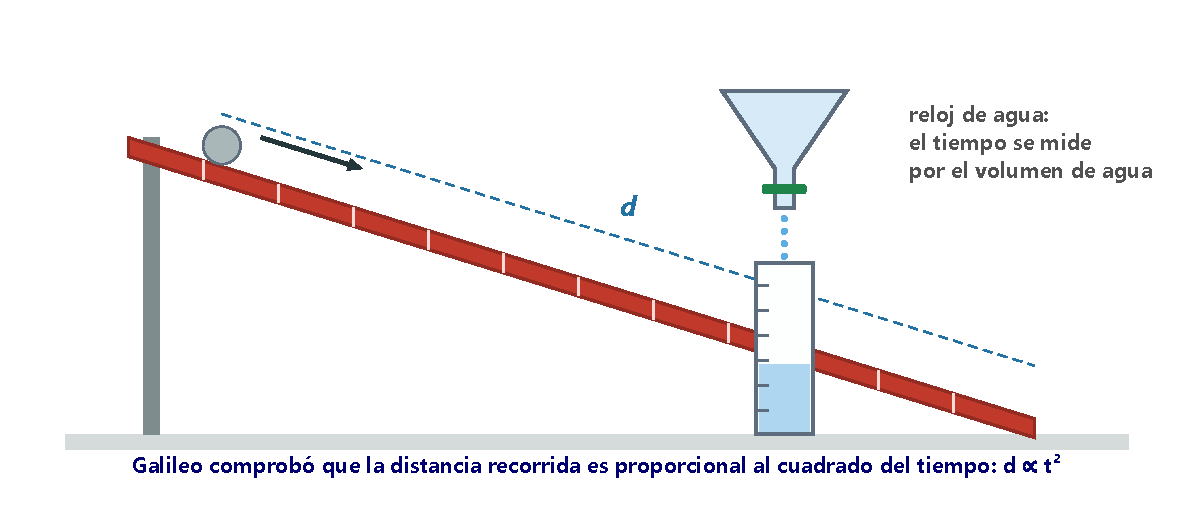
\includegraphics[width=0.6\textwidth]{images/UD9/plano_galileo}
    \caption{Reconstrucción del experimento de Galileo con el plano inclinado.}
    \label{fig:ud9-galileo}
\end{figure}

\begin{example}
    \textbf{Frenada.} Un conductor frena durante \qty{15}{\s} y recorre \qty{180}{\m} hasta pararse. Calcula: a) la velocidad que
    llevaba; b) la aceleración de frenado.

    \textbf{Solución.} Datos: \(t = \qty{15}{\s}\), \(\Delta x = \qty{180}{\m}\), \(v = 0\). Con las dos ecuaciones del MRUA:
    \[ 0 = v_0 + 15\,a \qquad\qquad 180 = 15\,v_0 + \frac{1}{2}\,a \cdot 15^2 \]
    De la primera, \(v_0 = -15\,a\); sustituyendo en la segunda, \(180 = -225\,a + \num{112.5}\,a = -\num{112.5}\,a\), de donde
    \(a = \qty{-1.6}{\m\per\s\squared}\) y \(v_0 = \qty{24}{\m\per\s}\) (\qty{86.4}{\km\per\hour}). (También se puede usar la
    velocidad media: \(v_m = \dfrac{v_0 + 0}{2} = \dfrac{180}{15} = \qty{12}{\m\per\s}\), así que \(v_0 = \qty{24}{\m\per\s}\).)
\end{example}

\begin{example}
    \textbf{¿Quién llega antes al autobús?} Marta corre hacia la parada del autobús, que está \qty{36}{\m} por delante de ella, a
    \qty{3}{\m\per\s} constantes. Su hermano Pablo, que está \qty{8}{\m} por detrás de ella, sale \qty{2}{\s} más tarde, desde el
    reposo, con una aceleración de \qty{1.2}{\m\per\s\squared}. a) ¿Quién llega antes a la parada? b) ¿A qué velocidad debería
    correr Marta para llegar a la vez que Pablo?

    \textbf{Solución.} Tomamos el origen en la posición inicial de Marta y \(t = 0\) cuando ella empieza a correr:
    \[ x_M = 3t \qquad\qquad x_P = -8 + \frac{1}{2} \cdot \num{1.2}\,(t - 2)^2 = -8 + \num{0.6}\,(t - 2)^2 \]
    a) Marta llega cuando \(3t = 36\): \(t = \qty{12}{\s}\). Pablo, cuando \(-8 + \num{0.6}(t - 2)^2 = 36\):
    \((t - 2)^2 = \num{73.3}\), \(t - 2 = \qty{8.56}{\s}\), \(t = \qty{10.56}{\s}\). \textbf{Pablo llega antes}, aunque salió más
    tarde y más lejos.

    b) Marta tendría que recorrer \qty{36}{\m} en \qty{10.56}{\s}: \(v = \dfrac{36}{\num{10.56}} = \qty{3.41}{\m\per\s}\).
\end{example}

\begin{exercise}
    Un móvil circula a \qty{20}{\m\per\s} y acelera a razón de \qty{4}{\m\per\s\squared}. Calcula: a) la velocidad y el espacio
    recorrido \qty{5}{\s} más tarde; b) la velocidad que tendrá cuando haya recorrido \qty{400}{\m}.
    \begin{solu}
        a) \(v = 20 + 4 \cdot 5 = \textcolor{red}{\qty{40}{\m\per\s}}\); \(\Delta x = 20 \cdot 5 + 2 \cdot 25 = \textcolor{red}{\qty{150}{\m}}\).
        b) \(v^2 = 400 + 2 \cdot 4 \cdot 400 = 3600\): \(\textcolor{red}{v = \qty{60}{\m\per\s}}\).
    \end{solu}
\end{exercise}

\begin{exercise}
    Villa Arriba y Villa Abajo están separadas por un camino recto de \qty{200}{\m}. Luis sale de Villa Abajo hacia Villa Arriba
    a \qty{4}{\m\per\s} y, como quiere llegar antes, acelera a \qty{0.5}{\m\per\s\squared}. A la vez, Ana sale de Villa Arriba
    hacia Villa Abajo a \qty{6}{\m\per\s} constantes. a) Escribe las ecuaciones de los dos movimientos y dibuja sus gráficas
    \(x\)-\(t\) y \(v\)-\(t\). b) ¿Cuándo y dónde se cruzan?
    \begin{solu}
        a) \textcolor{red}{\(x_L = 4t + 0{,}25\,t^2\); \(x_A = 200 - 6t\)}; \(v_L = 4 + 0{,}5\,t\) (recta creciente) y \(v_A = -6\)
        (recta horizontal). b) \(0{,}25\,t^2 + 10t - 200 = 0\): \(\textcolor{red}{t = \qty{14.6}{\s}}\), a
        \(\textcolor{red}{\qty{112}{\m}}\) de Villa Abajo.
    \end{solu}
\end{exercise}

\subsection{Movimiento vertical: caída libre}

Si dejamos caer o lanzamos un cuerpo en vertical y el rozamiento con el aire es despreciable, el cuerpo se mueve solo bajo la acción
de la gravedad: es un \textbf{movimiento de caída libre}, un caso particular de MRUA cuya aceleración es la \textbf{aceleración de la
gravedad}, \(\vec g\).

\begin{definition}[Aceleración de la gravedad]
    Cerca de la superficie terrestre, todos los cuerpos en caída libre tienen la misma aceleración, \(\vec g\), dirigida hacia el
    centro de la Tierra y de módulo \(g = \qty{9.8}{\m\per\s\squared}\), sea cual sea su masa.
\end{definition}

Tomamos el eje Y vertical y hacia arriba, con el origen en el suelo. Como \(\vec g\) apunta hacia abajo, \(a = -g\), y las ecuaciones
del MRUA quedan:
\[ \boxed{v_y = v_{0y} - g\,t} \qquad\qquad \boxed{y = y_0 + v_{0y}\,t - \frac{1}{2}\,g\,t^2} \qquad\qquad v_y^2 = v_{0y}^2 - 2\,g\,(y - y_0) \]
El signo negativo de \(g\) en las ecuaciones no depende de que el cuerpo suba o baje: la gravedad siempre tira hacia abajo.

\begin{itemize}
    \item \textbf{Se deja caer} (\(v_{0y} = 0\)) o \textbf{se lanza hacia abajo} (\(v_{0y} < 0\)): la velocidad es negativa durante
    toda la caída y su módulo aumenta.
    \item \textbf{Se lanza hacia arriba} (\(v_{0y} > 0\)), desde el suelo o desde cierta altura: \(v_y\) es positiva mientras sube,
    se anula en el punto más alto y es negativa mientras baja.
\end{itemize}

\textbf{Altura máxima.} En el punto más alto, \(v_y = 0\). El tiempo de subida se obtiene de \(0 = v_{0y} - g\,t_s\), es decir,
\(t_s = \dfrac{v_{0y}}{g}\), y la altura máxima, sustituyéndolo en la ecuación de la posición (o con
\(y_{\text{máx}} = y_0 + \dfrac{v_{0y}^2}{2g}\)). Si el cuerpo vuelve al mismo nivel desde el que se lanzó, tarda lo mismo en bajar que
en subir y llega con la misma rapidez con la que salió.

\begin{figure}[H]
    \centering
    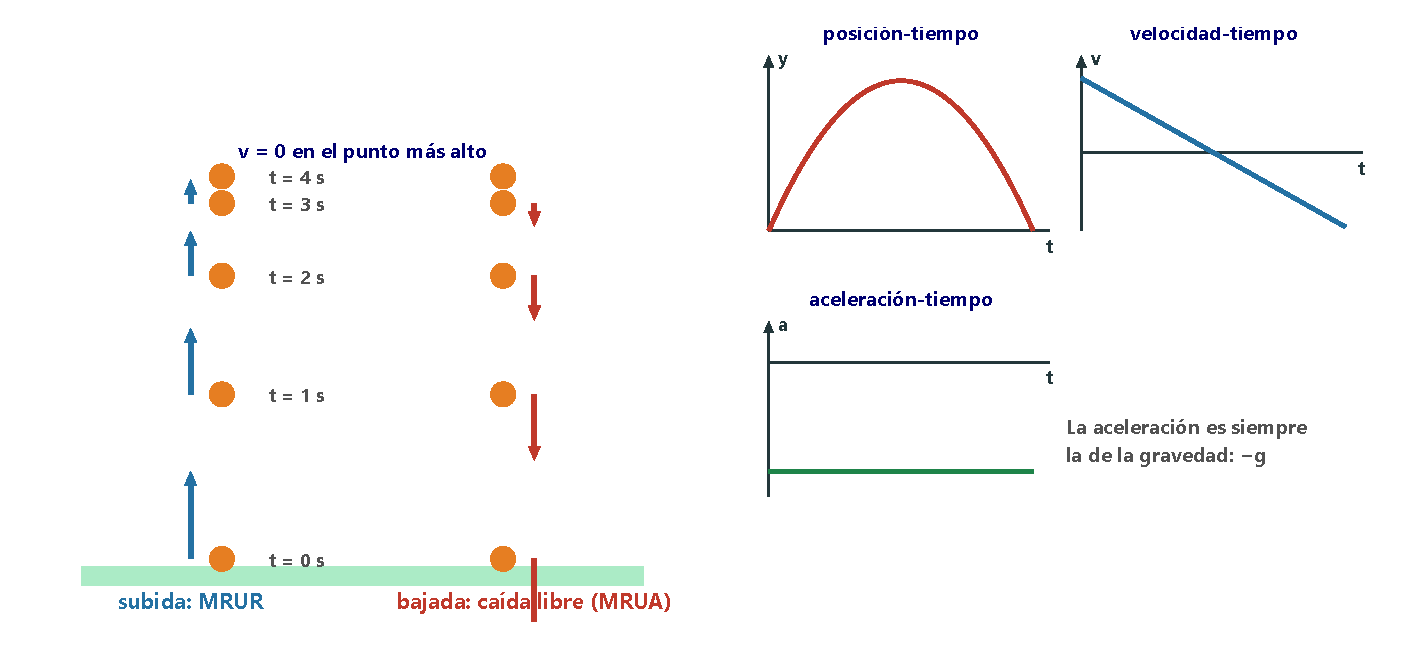
\includegraphics[width=0.95\textwidth]{images/UD9/lanzamiento_vertical}
    \caption{Lanzamiento vertical hacia arriba: subida con movimiento retardado, \(v = 0\) en el punto más alto, y bajada en caída
    libre. La aceleración es siempre \(-g\).}
    \label{fig:ud9-vertical}
\end{figure}

\begin{example}
    \textbf{Lanzamiento hacia arriba.} Pedro lanza una pelota hacia arriba a \qty{8}{\m\per\s}. Calcula: a) la altura máxima;
    b) el tiempo que está en el aire; c) la velocidad con la que vuelve a su mano.

    \textbf{Solución.} Origen en la mano: \(y = 8t - \num{4.9}\,t^2\) y \(v = 8 - \num{9.8}\,t\).
    a) En el punto más alto, \(v = 0\): \(t_s = \dfrac{8}{\num{9.8}} = \qty{0.816}{\s}\);
    \(y_{\text{máx}} = 8 \cdot \num{0.816} - \num{4.9} \cdot \num{0.816}^2 = \qty{3.27}{\m}\).
    b) Vuelve a \(y = 0\): \(t(8 - \num{4.9}\,t) = 0\), así que \(t = \qty{1.63}{\s}\), el doble del tiempo de subida.
    c) \(v = 8 - \num{9.8} \cdot \num{1.63} = \qty{-8}{\m\per\s}\): la misma rapidez, hacia abajo.
\end{example}

\begin{example}
    \textbf{Una herramienta desde un andamio.} Un andamio eléctrico sube a \qty{2}{\m\per\s} y, cuando está a \qty{30}{\m} de
    altura, se le cae una herramienta. Calcula: a) las ecuaciones de la posición y de la velocidad de la herramienta; b) cuánto tarda
    en llegar al suelo y con qué velocidad.

    \textbf{Solución.} a) La herramienta sale con la velocidad del andamio, \(v_0 = +\qty{2}{\m\per\s}\) (¡hacia arriba!):
    \(y = 30 + 2t - \num{4.9}\,t^2\) y \(v = 2 - \num{9.8}\,t\).
    b) Llega al suelo cuando \(y = 0\): \(\num{4.9}\,t^2 - 2t - 30 = 0\), con solución positiva \(t = \qty{2.69}{\s}\) (la negativa
    no tiene sentido físico). Entonces \(v = 2 - \num{9.8} \cdot \num{2.69} = \qty{-24.3}{\m\per\s}\): cae a \qty{24.3}{\m\per\s}.
\end{example}

\begin{example}
    \textbf{Encuentro en vertical.} Desde el suelo se lanza una llave hacia arriba a \qty{20}{\m\per\s} y, en el mismo instante, desde
    \qty{45}{\m} de altura se lanza una cerradura hacia abajo a \qty{8}{\m\per\s}. Calcula: a) cuándo y a qué altura se cruzan;
    b) dónde está la cerradura cuando la llave alcanza su altura máxima.

    \textbf{Solución.} \(y_1 = 20t - \num{4.9}\,t^2\) e \(y_2 = 45 - 8t - \num{4.9}\,t^2\).
    a) \(y_1 = y_2\): \(20t = 45 - 8t\) (¡los términos de \(t^2\) se anulan!), \(t = \qty{1.61}{\s}\), a una altura
    \(y = 20 \cdot \num{1.61} - \num{4.9} \cdot \num{1.61}^2 = \qty{19.5}{\m}\).
    b) La llave sube durante \(t = 20/\num{9.8} = \qty{2.04}{\s}\); entonces \(y_2 = 45 - 8 \cdot \num{2.04} - \num{4.9} \cdot
    \num{2.04}^2 = \qty{8.3}{\m}\): la cerradura todavía no ha llegado al suelo.
\end{example}

\begin{exercise}
    Se lanza un bolígrafo desde una ventana que está a \qty{25}{\m} de altura y tarda \qty{4}{\s} en llegar al suelo. ¿Con qué
    velocidad y en qué sentido se lanzó? Resuélvelo: a) tomando el origen en el suelo; b) tomando el origen en la ventana.
    \begin{solu}
        a) \(0 = 25 + 4\,v_0 - \num{4.9} \cdot 16\): \(\textcolor{red}{v_0 = \qty{13.4}{\m\per\s}}\), \textcolor{red}{hacia arriba}.
        b) \(-25 = 4\,v_0 - \num{78.4}\): el mismo resultado. El origen no cambia la física.
    \end{solu}
\end{exercise}

\begin{exercise}
    Desde lo alto de una torre de \qty{40}{\m} se lanza una caja verticalmente hacia arriba a \qty{10}{\m\per\s}. Calcula: a) su
    velocidad y su altura a los \qty{2}{\s}; b) la altura máxima y el tiempo que tarda en alcanzarla.
    \begin{solu}
        a) \(v = 10 - \num{19.6} = \textcolor{red}{\qty{-9.6}{\m\per\s}}\) (ya baja); \(y = 40 + 20 - \num{19.6} = \textcolor{red}{\qty{40.4}{\m}}\).
        b) \(\textcolor{red}{t = \qty{1.02}{\s}}\); \(y_{\text{máx}} = 40 + \dfrac{100}{\num{19.6}} = \textcolor{red}{\qty{45.1}{\m}}\).
    \end{solu}
\end{exercise}

%========================================================================================
\section{Composición de movimientos}\label{sec:ud9-composicion}
%========================================================================================

Muchos movimientos son la combinación de otros más sencillos: un kayak que cruza un río, una persona que camina por la cinta de un
aeropuerto o un balón lanzado a canasta. Para estudiarlos se usa una idea que ya aplicaba Galileo en el siglo \textsc{xvii}:

\begin{definition}[Principio de superposición]
    Cuando un cuerpo está sometido a varios movimientos simultáneos e independientes, el movimiento resultante se obtiene
    \textbf{sumando vectorialmente} las posiciones, velocidades y aceleraciones de cada uno de ellos, como si cada movimiento parcial
    ocurriera por separado. El \textbf{tiempo} es el mismo para todos los movimientos componentes.
\end{definition}

\subsection{Movimientos de la misma dirección}

Si los movimientos tienen la misma dirección, basta con sumar las velocidades con su signo:
\begin{itemize}
    \item \textbf{Dos MRU} dan un \textbf{MRU}, en el sentido del más rápido. Ejemplos: una persona que camina por una cinta
    transportadora o un salmón que remonta un río.
    \item Si \textbf{alguno es un MRUA}, el movimiento resultante es un \textbf{MRUA}. Ejemplo: un objeto que se deja caer dentro de
    un ascensor que sube con velocidad constante, visto desde fuera.
\end{itemize}

\begin{example}
    \textbf{En el aeropuerto.} Identifica el tipo de composición: a) arrancas a correr sobre una cinta transportadora para no perder
    el avión; b) nadas a \qty{1.2}{\m\per\s} a favor de la corriente de un río que fluye a \qty{0.5}{\m\per\s}.

    \textbf{Solución.} a) La cinta tiene un MRU y tú, sobre ella, un MRUA (arrancas desde el reposo): el resultado es un
    \textbf{MRUA}. b) Las dos velocidades son constantes y del mismo sentido: un \textbf{MRU} a \(\num{1.2} + \num{0.5} =
    \qty{1.7}{\m\per\s}\) respecto a la orilla.
\end{example}

\begin{exercise}
    a) Una pulga camina con rapidez constante sobre la cabeza de un perro que corre de forma uniforme por un sendero. b) En un globo
    aerostático que asciende con velocidad constante, juegas a lanzar una pelota hacia arriba y recogerla. Explica qué tipo de
    composición observa en cada caso una persona en reposo en el suelo.
    \begin{solu}
        a) \textcolor{red}{MRU + MRU = MRU}. b) \textcolor{red}{MRU (globo) + MRUA (pelota) = MRUA}: para la persona del suelo, la
        pelota sale con más velocidad (la suya más la del globo), pero su aceleración sigue siendo \(-g\).
    \end{solu}
\end{exercise}

\subsection{Movimientos perpendiculares}

\subsubsection{Composición de dos MRU: cruzar un río}

Una barca cruza un río remando con velocidad constante \(\vec v_n\) perpendicular a la orilla, mientras la corriente la arrastra con
velocidad \(\vec v_c\), también constante. Tomamos el eje X en la dirección de la corriente y el eje Y perpendicular a la orilla:
\[ x = v_c\,t \qquad y = v_n\,t \qquad \vec v = v_c\,\ivec + v_n\,\jvec \qquad |\vec v| = \sqrt{v_c^2 + v_n^2} \]
\begin{itemize}
    \item El \textbf{tiempo} que tarda en cruzar depende solo de la componente perpendicular: \(t = \dfrac{\text{anchura}}{v_n}\).
    La corriente no la retrasa.
    \item En ese tiempo, la corriente la arrastra río abajo una distancia \(x = v_c\,t\).
    \item La trayectoria es una recta, \(y = \dfrac{v_n}{v_c}\,x\), que forma con la corriente un ángulo \(\alpha\) tal que
    \(\tg\alpha = \dfrac{v_n}{v_c}\).
\end{itemize}

\begin{figure}[H]
    \centering
    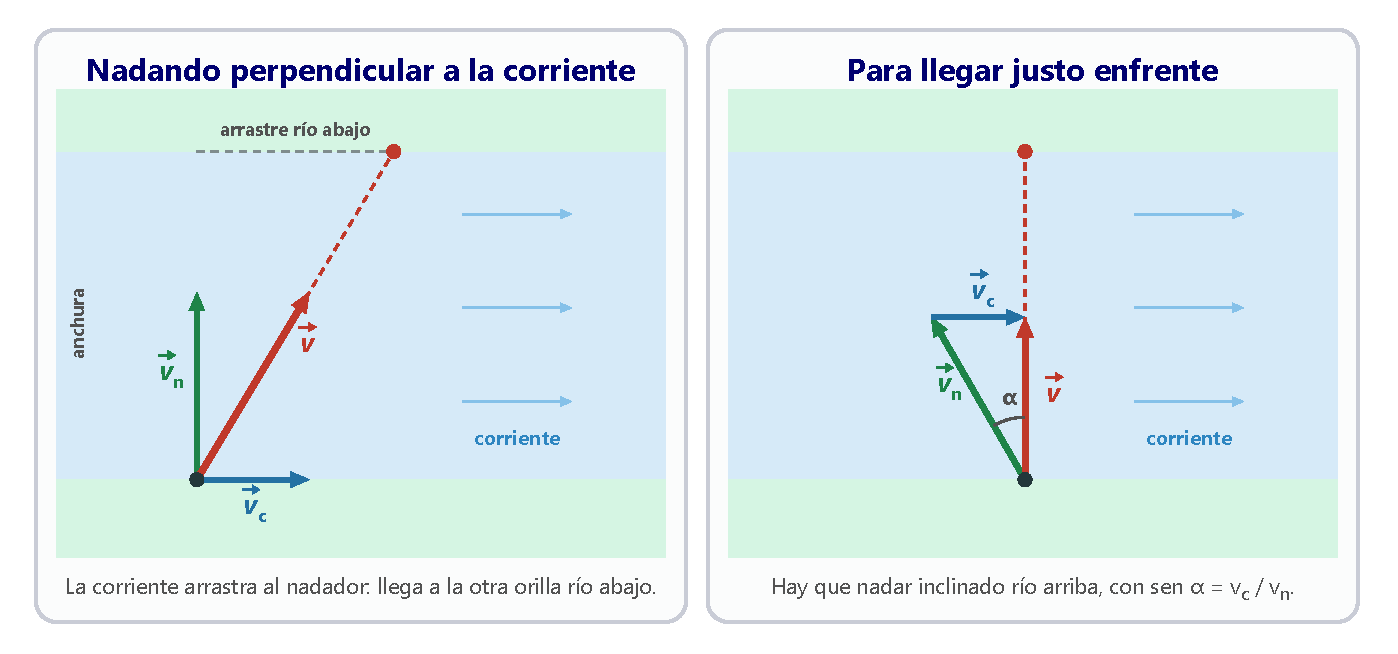
\includegraphics[width=0.9\textwidth]{images/UD9/composicion_rio}
    \caption{Composición de dos MRU perpendiculares: la velocidad real es la suma vectorial de la propia y la de la corriente.}
    \label{fig:ud9-rio}
\end{figure}

\begin{example}
    \textbf{Llegar justo enfrente.} Un río de \qty{24}{\m} de ancho lleva una corriente de \qty{2}{\m\per\s}. Un nadador puede
    nadar a \qty{4}{\m\per\s} respecto al agua. ¿En qué dirección debe nadar para llegar justo enfrente? ¿Cuánto tardará?

    \textbf{Solución.} Debe nadar inclinado río arriba, de modo que la componente de su velocidad paralela a la orilla anule la
    corriente (figura~\ref{fig:ud9-rio}, derecha). Si \(\alpha\) es el ángulo con la perpendicular a la orilla:
    \[ \sen\alpha = \frac{v_c}{v_n} = \frac{2}{4} = \num{0.5} \quad\Rightarrow\quad \alpha = 30^\circ \text{ río arriba} \]
    Su velocidad real es perpendicular a la orilla, de módulo \(v = \sqrt{4^2 - 2^2} = \qty{3.46}{\m\per\s}\), y tarda
    \(t = \dfrac{24}{\num{3.46}} = \qty{6.93}{\s}\).
\end{example}

\begin{exercise}
    Se quiere cruzar un río de \qty{40}{\m} de ancho nadando a \qty{2}{\m\per\s} perpendicularmente a una corriente de
    \qty{1.2}{\m\per\s}. Calcula: a) la velocidad real del nadador respecto a la orilla; b) el ángulo que forma con la corriente;
    c) el tiempo que tarda en llegar a la otra orilla; d) la distancia que lo arrastra la corriente.
    \begin{solu}
        a) \(\sqrt{4 + \num{1.44}} = \textcolor{red}{\qty{2.33}{\m\per\s}}\); b) \(\tg\alpha = \dfrac{2}{\num{1.2}}\):
        \(\textcolor{red}{\alpha = 59^\circ}\); c) \(\dfrac{40}{2} = \textcolor{red}{\qty{20}{\s}}\); d) \(\num{1.2} \cdot 20 =
        \textcolor{red}{\qty{24}{\m}}\) río abajo.
    \end{solu}
\end{exercise}

\subsubsection{Tiro parabólico: composición de un MRU y un MRUA}

\begin{definition}[Tiro parabólico u oblicuo]
    Es el movimiento de un cuerpo lanzado con una velocidad inicial \(\vec v_0\) que forma un ángulo \(\alpha\) con la horizontal y que
    se mueve después solo bajo la acción de la gravedad (despreciamos el rozamiento con el aire). Su trayectoria es una
    \textbf{parábola}.
\end{definition}

Ejemplos: el saque de un balón de voleibol, un golpe de golf o el salto de una moto en una rampa. Descomponemos la velocidad inicial
en una componente horizontal y otra vertical:
\[ v_{0x} = v_0\cos\alpha \qquad\qquad v_{0y} = v_0\,\sen\alpha \]
\begin{itemize}
    \item En el eje X no hay aceleración: el movimiento horizontal es un \textbf{MRU} con velocidad \(v_{0x}\), que produce el avance.
    \item En el eje Y la aceleración es \(-g\): el movimiento vertical es un \textbf{MRUA} (un lanzamiento vertical) con velocidad
    inicial \(v_{0y}\), que produce la subida y la bajada.
\end{itemize}

\begin{figure}[H]
    \centering
    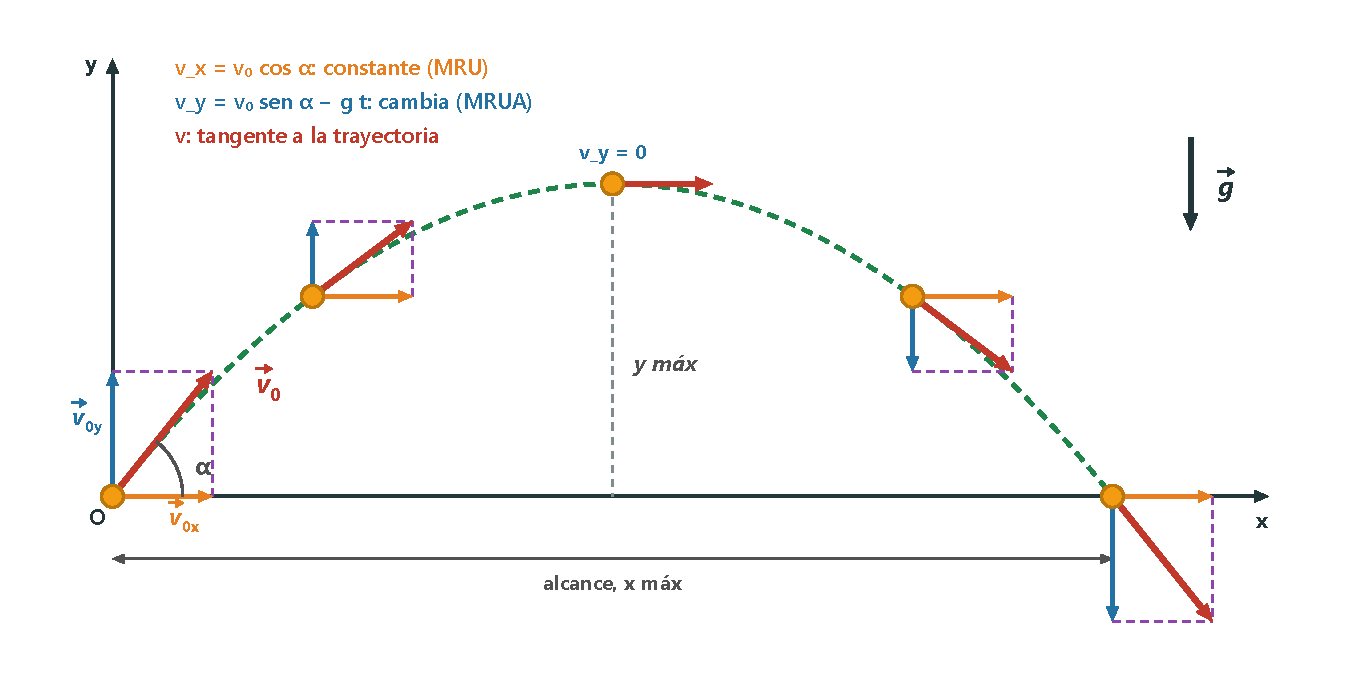
\includegraphics[width=0.95\textwidth]{images/UD9/tiro_parabolico}
    \caption{En el tiro parabólico, la componente horizontal de la velocidad es constante y la vertical cambia como en un lanzamiento
    vertical.}
    \label{fig:ud9-parabolico}
\end{figure}

Con el origen en el suelo, en la vertical del punto de lanzamiento, y la posición inicial \((0, y_0)\):

\begin{table}[H]
    \centering
    \caption{Ecuaciones del tiro parabólico}
    \vspace{-5pt}
    \begin{tabular}{@{}lL{9cm}@{}}
        \toprule
        \textbf{Magnitud} & \textbf{Ecuación} \\
        \midrule
        Posición & \(x = v_0\cos\alpha\,t\) \qquad \(y = y_0 + v_0\,\sen\alpha\,t - \frac{1}{2}\,g\,t^2\) \\[3pt]
        Velocidad & \(v_x = v_0\cos\alpha\) (constante) \qquad \(v_y = v_0\,\sen\alpha - g\,t\) \\[3pt]
        Vectores & \(\vec r = x\,\ivec + y\,\jvec\) \qquad \(\vec v = v_x\,\ivec + v_y\,\jvec\) \qquad \(\vec a = -g\,\jvec\) \\[3pt]
        Trayectoria & \(y = y_0 + x\,\tg\alpha - \dfrac{g}{2\,v_0^2\cos^2\alpha}\,x^2\) (una parábola) \\
        \bottomrule
    \end{tabular}
    \label{tab:ud9-parabolico}
\end{table}

Tres magnitudes caracterizan el lanzamiento:
\begin{itemize}
    \item \textbf{Tiempo de vuelo}: el que tarda en llegar al suelo, cuando \(y = 0\). Si se lanzó desde el suelo (\(y_0 = 0\)):
    \(t_{\text{vuelo}} = \dfrac{2\,v_0\,\sen\alpha}{g}\).
    \item \textbf{Altura máxima}: en ella, \(v_y = 0\). Desde el suelo: \(y_{\text{máx}} = \dfrac{v_0^2\,\sen^2\alpha}{2g}\).
    \item \textbf{Alcance}: la distancia horizontal recorrida hasta tocar el suelo, \(x_{\text{máx}} = v_0\cos\alpha\,t_{\text{vuelo}}\).
    Desde el suelo: \(x_{\text{máx}} = \dfrac{v_0^2\,\sen 2\alpha}{g}\). El alcance es máximo para \(\alpha = 45^\circ\), y dos
    ángulos complementarios (\(30^\circ\) y \(60^\circ\), por ejemplo) dan el mismo alcance.
\end{itemize}
Si el cuerpo se lanza desde cierta altura o choca con un obstáculo, no se pueden usar estas fórmulas abreviadas: hay que plantear las
ecuaciones de la tabla~\ref{tab:ud9-parabolico}.

\begin{example}
    \textbf{Un proyectil.} Se lanza un proyectil desde el suelo a \qty{80}{\m\per\s} con una inclinación de \(35^\circ\) sobre la
    horizontal. Despreciando el rozamiento con el aire, calcula: a) la altura máxima; b) a qué distancia horizontal del punto de
    lanzamiento la alcanza; c) el alcance.

    \textbf{Solución.} Componentes de la velocidad inicial: \(v_{0x} = 80\cos 35^\circ = \qty{65.5}{\m\per\s}\) y
    \(v_{0y} = 80\,\sen 35^\circ = \qty{45.9}{\m\per\s}\). Ecuaciones: \(x = \num{65.5}\,t\); \(y = \num{45.9}\,t - \num{4.9}\,t^2\);
    \(v_y = \num{45.9} - \num{9.8}\,t\).

    a) En el punto más alto, \(v_y = 0\): \(t = \dfrac{\num{45.9}}{\num{9.8}} = \qty{4.68}{\s}\), y
    \(y_{\text{máx}} = \num{45.9} \cdot \num{4.68} - \num{4.9} \cdot \num{4.68}^2 = \qty{107}{\m}\).
    b) \(x = \num{65.5} \cdot \num{4.68} = \qty{307}{\m}\).
    c) Llega al suelo cuando \(y = 0\): \(t(\num{45.9} - \num{4.9}\,t) = 0\), \(t = \qty{9.36}{\s}\) (el doble que la subida), y
    \(x_{\text{máx}} = \num{65.5} \cdot \num{9.36} = \qty{614}{\m}\). Con la fórmula: \(\dfrac{80^2\,\sen 70^\circ}{\num{9.8}} =
    \qty{614}{\m}\).
\end{example}

\begin{exercise}
    Andrea juega al golf y está a \qty{250}{\m} del hoyo. Va a golpear la pelota con un ángulo de \(30^\circ\) con la horizontal.
    a) ¿Con qué velocidad debe salir la pelota para caer en el hoyo? b) ¿Cuánto tiempo estará en el aire?
    \begin{solu}
        a) \(250 = \dfrac{v_0^2\,\sen 60^\circ}{\num{9.8}}\): \(\textcolor{red}{v_0 = \qty{53.2}{\m\per\s}}\).
        b) \(t = \dfrac{2 \cdot \num{53.2} \cdot \sen 30^\circ}{\num{9.8}} = \textcolor{red}{\qty{5.43}{\s}}\).
    \end{solu}
\end{exercise}

\begin{exercise}
    Una futbolista lanza una falta a \qty{25}{\m\per\s} con un ángulo de \(25^\circ\). Si el balón no tocara a nadie ni la portería,
    ¿cuánto tiempo estaría en el aire? ¿A qué distancia caería? ¿Qué altura máxima alcanzaría?
    \begin{solu}
        \(t = \dfrac{2 \cdot 25\,\sen 25^\circ}{\num{9.8}} = \textcolor{red}{\qty{2.16}{\s}}\); \(x = \dfrac{625\,\sen 50^\circ}{\num{9.8}} =
        \textcolor{red}{\qty{48.9}{\m}}\); \(y_{\text{máx}} = \dfrac{625\,\sen^2 25^\circ}{\num{19.6}} = \textcolor{red}{\qty{5.70}{\m}}\).
    \end{solu}
\end{exercise}

\begin{exercise}
    Con un laboratorio virtual de tiro parabólico (o con las fórmulas), completa estas tablas y saca conclusiones. a) Con \(\alpha =
    45^\circ\), calcula el alcance para \(v_0 = 5\), 8, 11, 14, 17 y \qty{20}{\m\per\s}. b) Con \(v_0 = \qty{15}{\m\per\s}\), calcula el
    alcance para \(\alpha = 25^\circ\), \(35^\circ\), \(45^\circ\), \(55^\circ\), \(65^\circ\) y \(75^\circ\).
    \begin{solu}
        a) \(x = v_0^2/g\): \textcolor{red}{2,55; 6,53; 12,3; 20,0; 29,5 y \qty{40.8}{\m}}: \textcolor{red}{el alcance es proporcional
        al cuadrado de la velocidad}. b) \(x = 225\,\sen 2\alpha/\num{9.8}\): \textcolor{red}{17,6; 21,6; 23,0; 21,6; 17,6 y
        \qty{11.5}{\m}}: \textcolor{red}{máximo a \(45^\circ\); ángulos complementarios dan el mismo alcance}.
    \end{solu}
\end{exercise}

\subsubsection{Tiro horizontal}

\begin{definition}[Tiro horizontal]
    Es el movimiento de un cuerpo lanzado desde una altura \(y_0\) con una velocidad inicial \(\vec v_0\) \textbf{horizontal}. Es el
    caso particular del tiro parabólico con \(\alpha = 0\): \(v_{0x} = v_0\) y \(v_{0y} = 0\).
\end{definition}

Ejemplos: una gota de rocío que se desliza por una hoja y cae, o un paquete de ayuda humanitaria que se suelta desde un avión que
vuela en horizontal. Las ecuaciones son:
\[ x = v_0\,t \qquad y = y_0 - \frac{1}{2}\,g\,t^2 \qquad v_x = v_0 \qquad v_y = -g\,t \qquad
   \text{trayectoria: } y = y_0 - \frac{g}{2\,v_0^2}\,x^2 \]

\begin{figure}[H]
    \centering
    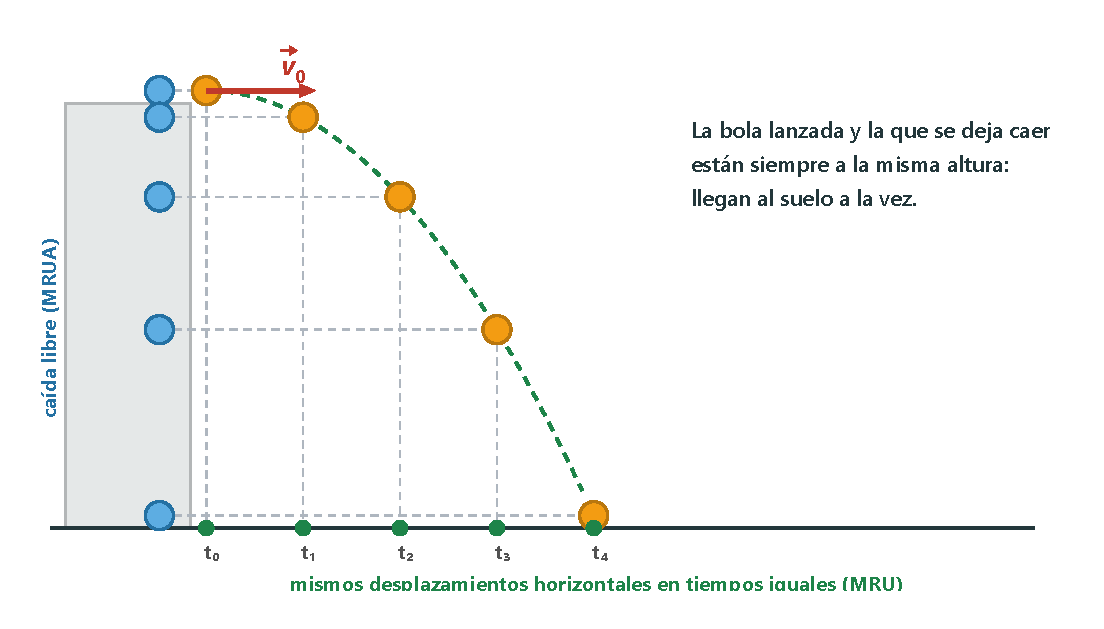
\includegraphics[width=0.75\textwidth]{images/UD9/tiro_horizontal}
    \caption{Una bola lanzada horizontalmente y otra que se deja caer a la vez desde la misma altura llegan juntas al suelo.}
    \label{fig:ud9-horizontal}
\end{figure}

\begin{remark}
    \textbf{Todos llegan a la vez.} El lanzamiento vertical, el horizontal y el parabólico son movimientos de caída libre. Por eso, los
    cuerpos que caen desde la misma altura máxima tardan exactamente lo mismo en llegar al suelo, tanto si se dejan caer como si se
    lanzan horizontalmente: el movimiento horizontal no influye en el vertical.
\end{remark}

\begin{example}
    \textbf{La flecha y la manzana.} Un arquero lanza una flecha horizontalmente desde un puente de \qty{20}{\m} de altura a
    \qty{12}{\m\per\s}, y en el mismo instante se deja caer una manzana desde el mismo puente. Despreciando el rozamiento, calcula:
    a) el tiempo que la flecha está en el aire; b) a qué distancia del puente cae; c) su velocidad y su ángulo al llegar al agua;
    d) ¿cuál llega antes al agua y cuál lo hace más rápido?

    \textbf{Solución.} Flecha: \(x = 12t\); \(y = 20 - \num{4.9}\,t^2\); \(v_x = 12\); \(v_y = -\num{9.8}\,t\).
    a) \(y = 0\): \(t = \sqrt{\dfrac{20}{\num{4.9}}} = \qty{2.02}{\s}\). b) \(x = 12 \cdot \num{2.02} = \qty{24.2}{\m}\).
    c) \(v_y = -\num{9.8} \cdot \num{2.02} = \qty{-19.8}{\m\per\s}\); \(\vec v = (12\,\ivec - \num{19.8}\,\jvec)~\unit{\m\per\s}\), de módulo
    \(\sqrt{144 + 392} = \qty{23.2}{\m\per\s}\). El ángulo con la horizontal es \(\alpha = \arctg\dfrac{\num{19.8}}{12} = 58.8^\circ\),
    por debajo de ella.
    d) La manzana cumple \(y = 20 - \num{4.9}\,t^2\), igual que la flecha: \textbf{llegan a la vez}. Pero la manzana llega a
    \qty{19.8}{\m\per\s}, más despacio que la flecha, porque no tiene componente horizontal.
\end{example}

\begin{exercise}
    a) Un pájaro que vuela horizontalmente a \qty{25}{\m\per\s} suelta una ramita. Escribe la velocidad de la ramita en función del
    tiempo. b) Desde un helicóptero que avanza horizontalmente a \qty{30}{\m\per\s} a \qty{150}{\m} de altura cae un objeto. Escribe
    su componente vertical de la posición, su vector posición y su componente vertical de la velocidad.
    \begin{solu}
        a) \(\textcolor{red}{\vec v = (25\,\ivec - \num{9.8}\,t\,\jvec)~\unit{\m\per\s}}\). b) \(\textcolor{red}{y = 150 - \num{4.9}\,t^2}\);
        \(\textcolor{red}{\vec r = 30t\,\ivec + (150 - \num{4.9}\,t^2)\,\jvec~\unit{\m}}\); \(\textcolor{red}{v_y = -\num{9.8}\,t~\unit{\m\per\s}}\).
    \end{solu}
\end{exercise}

\begin{exercise}
    Se lanza horizontalmente una pelota a \qty{8}{\m\per\s} desde \qty{25}{\m} de altura. Calcula: a) los vectores velocidad y
    posición; b) a qué distancia cae.
    \begin{solu}
        a) \(\textcolor{red}{\vec v = 8\,\ivec - \num{9.8}\,t\,\jvec}\); \(\textcolor{red}{\vec r = 8t\,\ivec + (25 - \num{4.9}\,t^2)\,\jvec}\).
        b) \(t = \sqrt{25/\num{4.9}} = \qty{2.26}{\s}\); \(x = \textcolor{red}{\qty{18.1}{\m}}\).
    \end{solu}
\end{exercise}

\begin{exercise}
    Joseba juega al pádel en una pista de \qty{20}{\m} de largo con la red, de \qty{0.88}{\m}, en el centro. Golpea la pelota
    horizontalmente a \qty{80}{\km\per\hour} desde el fondo de la pista y a \qty{1.9}{\m} de altura. a) ¿A qué altura llega la
    pelota a la red? ¿Pasa por encima? b) ¿Cuánto tiempo está en el aire y a qué distancia del fondo contrario bota?
    \begin{solu}
        a) \textcolor{blue}{\(v_0 = \qty{22.2}{\m\per\s}\); llega a la red (\(x = 10\)) en \(t = \qty{0.45}{\s}\).}
        \(y = \num{1.9} - \num{4.9} \cdot \num{0.45}^2 = \textcolor{red}{\qty{0.91}{\m}}\): \textcolor{red}{pasa por muy poco}.
        b) \(t = \sqrt{\num{1.9}/\num{4.9}} = \textcolor{red}{\qty{0.62}{\s}}\); \(x = \qty{13.8}{\m}\): bota a
        \(\textcolor{red}{\qty{6.2}{\m}}\) del fondo contrario.
    \end{solu}
\end{exercise}

%========================================================================================
\section{El movimiento circular}\label{sec:ud9-circular}
%========================================================================================

\begin{definition}[Movimiento circular]
    Un \textbf{movimiento circular} es aquel cuya trayectoria es una circunferencia.
\end{definition}

Son movimientos circulares los de las aspas de un aerogenerador, un tiovivo, la rueda de una jaula de hámster o un punto de un CD.
Conviene colocar el origen del sistema de referencia en el centro de la circunferencia: así, el módulo del vector posición es
siempre el radio \(R\) y solo cambia su dirección, que se describe con el ángulo \(\varphi\) que forma con el eje X. Por eso el
movimiento circular se describe muy bien con \textbf{magnitudes angulares}.

\subsection{Magnitudes angulares}

\begin{table}[H]
    \centering
    \caption{Magnitudes angulares del movimiento circular}
    \vspace{-5pt}
    \begin{tabular}{@{}lL{9.5cm}@{}}
        \toprule
        \textbf{Magnitud} & \textbf{Definición} \\
        \midrule
        Posición angular, \(\varphi\) & Ángulo que forma el vector posición con el semieje X positivo. Se mide en radianes (rad) \\[3pt]
        Desplazamiento angular, \(\Delta\varphi\) & Ángulo girado entre dos instantes: \(\Delta\varphi = \varphi - \varphi_0\) (rad) \\[3pt]
        Velocidad angular media, \(\omega_m\) & \(\omega_m = \dfrac{\Delta\varphi}{\Delta t}\), en \unit{\radian\per\s} \\[8pt]
        Velocidad angular, \(\omega\) & \(\omega = \dfrac{\dif\varphi}{\dif t}\), en \unit{\radian\per\s}. Es positiva en sentido antihorario y negativa en el horario \\[8pt]
        Aceleración angular, \(\alpha\) & \(\alpha = \dfrac{\dif\omega}{\dif t}\), en \unit{\radian\per\s\squared} \\
        \bottomrule
    \end{tabular}
    \label{tab:ud9-angulares}
\end{table}

\begin{figure}[H]
    \centering
    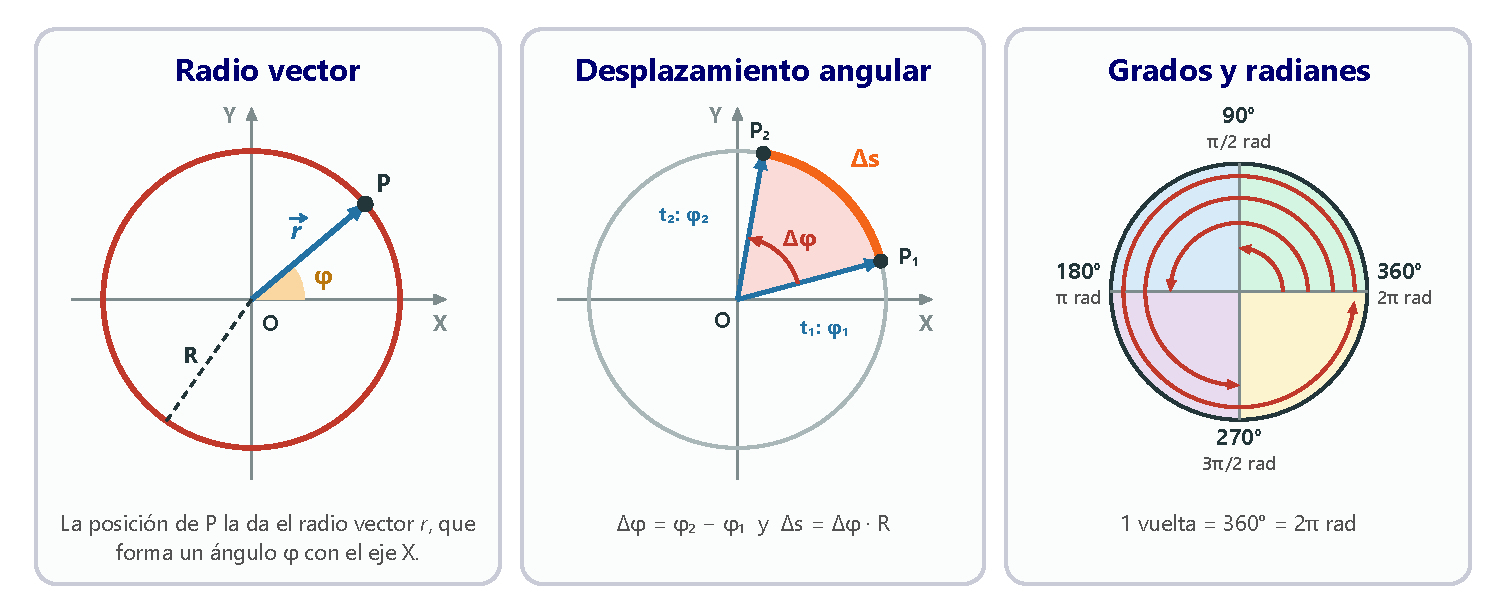
\includegraphics[width=0.95\textwidth]{images/UD9/mcu_magnitudes}
    \caption{Posición angular, desplazamiento angular y equivalencia entre grados y radianes.}
    \label{fig:ud9-angulares}
\end{figure}

\subsubsection{Relación entre las magnitudes angulares y las lineales}

El radio es el factor que relaciona las magnitudes angulares con las lineales (las medidas sobre la trayectoria):
\[ \Delta s = R\,\Delta\varphi \qquad\qquad v = R\,\omega \qquad\qquad a_t = R\,\alpha \]
Todos los puntos de un disco que gira tienen la misma velocidad angular, pero los más alejados del centro tienen más velocidad
lineal: recorren un arco más largo en el mismo tiempo.

\begin{figure}[H]
    \centering
    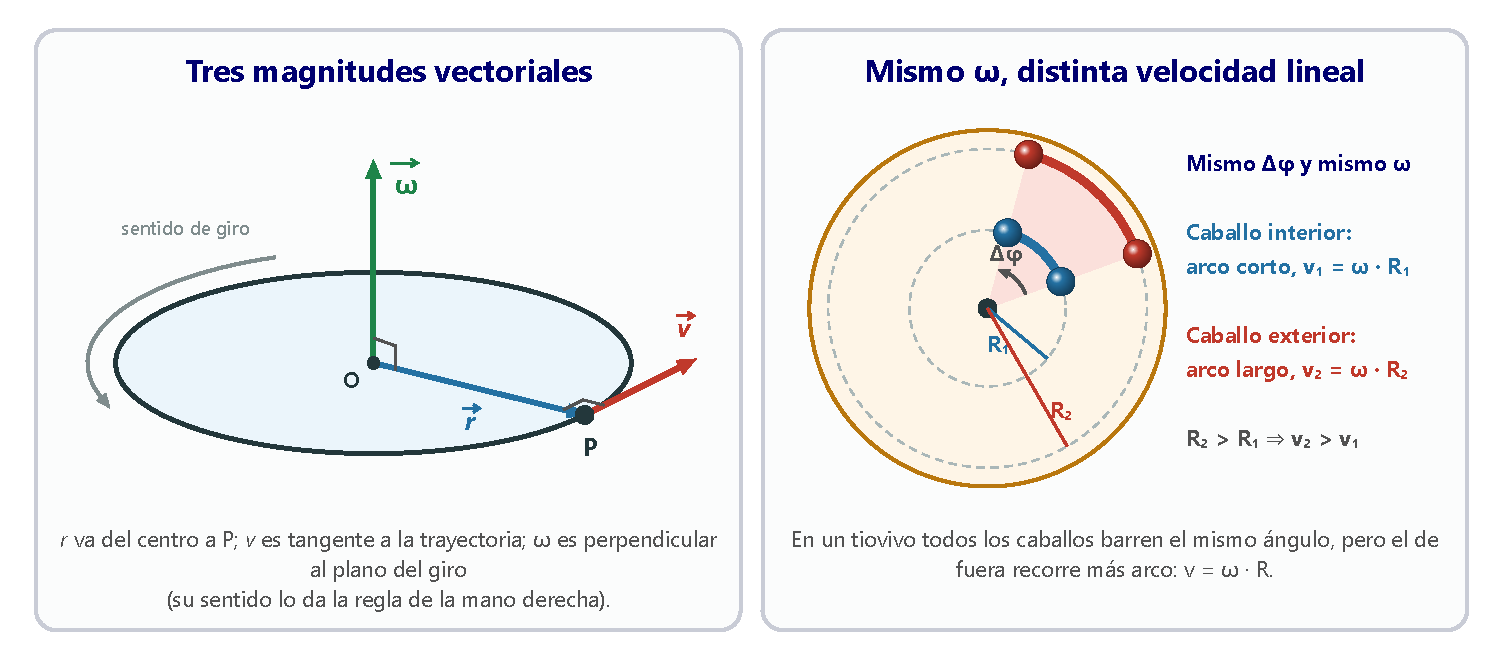
\includegraphics[width=0.95\textwidth]{images/UD9/mcu_vectores}
    \caption{En un tiovivo todos los caballos giran con la misma \(\omega\), pero los exteriores van más deprisa.}
    \label{fig:ud9-vectores}
\end{figure}

\begin{example}
    \textbf{Una plataforma giratoria.} Una plataforma de \qty{40}{\cm} de radio da 4 vueltas cada minuto. ¿Cuál es su velocidad
    angular? ¿Y la velocidad lineal de un punto del borde?

    \textbf{Solución.} \(\omega = 4~\dfrac{\text{vueltas}}{\unit{\minute}} \cdot \dfrac{2\pi~\text{rad}}{1~\text{vuelta}} \cdot
    \dfrac{\qty{1}{\minute}}{\qty{60}{\s}} = \dfrac{2\pi}{15} = \qty{0.419}{\radian\per\s}\);
    \(v = \omega\,R = \num{0.419} \cdot \num{0.40} = \qty{0.168}{\m\per\s}\).
\end{example}

\subsection{Movimiento circular uniforme (MCU)}

\begin{definition}[MCU]
    En el \textbf{movimiento circular uniforme} la trayectoria es una circunferencia y la rapidez es constante, es decir, la
    \textbf{velocidad angular \(\omega\) es constante}.
\end{definition}

Como \(\omega\) es constante, coincide con la media; despejando la posición angular (con \(t_0 = 0\)) obtenemos la ecuación del MCU:
\[ \boxed{\varphi = \varphi_0 + \omega\,t} \]
\begin{itemize}
    \item La rapidez es constante, así que \textbf{no hay aceleración tangencial}: \(a_t = 0\) y \(\alpha = 0\).
    \item La dirección de la velocidad cambia continuamente, así que \textbf{sí hay aceleración normal}, dirigida hacia el centro y
    de módulo constante: \(\boxed{a_n = \dfrac{v^2}{R} = \omega^2\,R}\).
\end{itemize}

\subsubsection{El MCU es periódico}

El MCU es un \textbf{movimiento periódico}: la posición, la velocidad y la aceleración se repiten cada vez que el móvil da una vuelta.
\begin{itemize}
    \item El \textbf{periodo}, \(T\), es el tiempo que tarda en dar una vuelta completa (en girar \(2\pi\)~rad). Se mide en segundos.
    \item La \textbf{frecuencia}, \(f\), es el número de vueltas por unidad de tiempo. Se mide en \unit{\per\s}, que se llama
    \textbf{hercio} (Hz).
\end{itemize}
\[ \boxed{T = \frac{2\pi}{\omega}} \qquad\qquad \boxed{f = \frac{1}{T} = \frac{\omega}{2\pi}} \]

\begin{remark}
    \textbf{Paralelismo entre los movimientos uniformes.} En el MRU, \(\Delta x = v\,t\) con \(v\) constante; en el MCU,
    \(\Delta s = v\,t\) con la rapidez constante y, en magnitudes angulares, \(\Delta\varphi = \omega\,t\) con \(\omega\) constante.
\end{remark}

\begin{example}
    \textbf{La Luna.} La Luna da una vuelta alrededor de la Tierra en \num{27.3} días, a una distancia media de
    \qty{3.84e8}{\m}. Suponiendo que su órbita es circular, calcula: a) su periodo en segundos, su frecuencia y su velocidad angular;
    b) su aceleración normal.

    \textbf{Solución.} a) \(T = \num{27.3}~\text{días} \cdot \dfrac{\qty{24}{\hour}}{1~\text{día}} \cdot \dfrac{\qty{3600}{\s}}{\qty{1}{\hour}} =
    \qty{2.36e6}{\s}\); \(f = \dfrac{1}{T} = \qty{4.24e-7}{\hertz}\); \(\omega = \dfrac{2\pi}{T} = \qty{2.66e-6}{\radian\per\s}\).
    b) \(a_n = \omega^2\,R = (\num{2.66e-6})^2 \cdot \num{3.84e8} = \qty{2.72e-3}{\m\per\s\squared}\), unas \num{3600} veces menor que
    \(g\): fue una de las pistas que llevaron a Newton a su ley de la gravitación.
\end{example}

\begin{exercise}
    Las palas de un aerogenerador miden \qty{30}{\m} y giran a 15 vueltas por minuto. Calcula: a) la velocidad angular, el periodo y
    la frecuencia; b) la velocidad lineal y la aceleración normal del extremo de una pala.
    \begin{solu}
        a) \(\textcolor{red}{\omega = \qty{1.57}{\radian\per\s}}\); \(\textcolor{red}{T = \qty{4}{\s}}\); \(\textcolor{red}{f = \qty{0.25}{\hertz}}\).
        b) \(v = \num{1.57} \cdot 30 = \textcolor{red}{\qty{47.1}{\m\per\s}}\) (\qty{170}{\km\per\hour}); \(a_n = \num{1.57}^2 \cdot 30 =
        \textcolor{red}{\qty{74.0}{\m\per\s\squared}}\).
    \end{solu}
\end{exercise}

\subsection{Movimiento circular uniformemente acelerado (MCUA)}

\begin{definition}[MCUA]
    En el \textbf{movimiento circular uniformemente acelerado} la trayectoria es una circunferencia y la \textbf{aceleración angular
    \(\alpha\) es constante}.
\end{definition}

Ahora cambian tanto la dirección como el módulo de la velocidad, así que hay los dos tipos de aceleración:
\begin{itemize}
    \item \textbf{aceleración tangencial}, constante: \(a_t = \alpha\,R\);
    \item \textbf{aceleración normal}, que crece o disminuye con la velocidad: \(a_n = \dfrac{v^2}{R} = \omega^2 R\).
\end{itemize}
Las ecuaciones del MCUA son las del MRUA cambiando las magnitudes lineales por las angulares (con \(t_0 = 0\)):
\[ \boxed{\omega = \omega_0 + \alpha\,t} \qquad\qquad \boxed{\varphi = \varphi_0 + \omega_0\,t + \frac{1}{2}\,\alpha\,t^2}
   \qquad\qquad \omega^2 = \omega_0^2 + 2\,\alpha\,(\varphi - \varphi_0) \]
Si \(\omega\) aumenta, \(\alpha > 0\); si disminuye, \(\alpha < 0\). El MCUA \textbf{no es periódico}: no tiene sentido hablar de su
periodo ni de su frecuencia.

\begin{table}[H]
    \centering
    \caption{Comparación entre las ecuaciones del MRUA y del MCUA}
    \vspace{-5pt}
    \begin{tabular}{@{}lccc@{}}
        \toprule
        \textbf{Movimiento} & \textbf{Velocidad} & \textbf{Posición} & \textbf{Sin el tiempo} \\
        \midrule
        MRUA & \(v = v_0 + a\,t\) & \(x = x_0 + v_0\,t + \frac{1}{2}\,a\,t^2\) & \(v^2 = v_0^2 + 2\,a\,\Delta x\) \\[3pt]
        MCUA (lineales) & \(v = v_0 + a_t\,t\) & \(s = s_0 + v_0\,t + \frac{1}{2}\,a_t\,t^2\) & \(v^2 = v_0^2 + 2\,a_t\,\Delta s\) \\[3pt]
        MCUA (angulares) & \(\omega = \omega_0 + \alpha\,t\) & \(\varphi = \varphi_0 + \omega_0\,t + \frac{1}{2}\,\alpha\,t^2\) & \(\omega^2 = \omega_0^2 + 2\,\alpha\,\Delta\varphi\) \\
        \bottomrule
    \end{tabular}
    \label{tab:ud9-mcua}
\end{table}

\begin{example}
    \textbf{Las ruedas de un coche.} Un coche acelera de 0 a \qty{90}{\km\per\hour} en \qty{8}{\s}. Sus ruedas tienen \qty{60}{\cm}
    de diámetro. Calcula: a) la aceleración angular de las ruedas; b) las vueltas que dan en esos \qty{8}{\s} y la distancia que
    recorre el coche; c) la velocidad angular de las ruedas a los \qty{15}{\s}, si siguiera acelerando igual.

    \textbf{Solución.} \(v = \qty{25}{\m\per\s}\) y \(R = \qty{0.30}{\m}\). a) \(\omega = \dfrac{v}{R} = \dfrac{25}{\num{0.30}} =
    \qty{83.3}{\radian\per\s}\); \(\alpha = \dfrac{\num{83.3} - 0}{8} = \qty{10.4}{\radian\per\s\squared}\).
    b) \(\Delta\varphi = \dfrac{1}{2} \cdot \num{10.4} \cdot 8^2 = \qty{333}{\radian}\), es decir, \(\dfrac{333}{2\pi} = \num{53}\)
    vueltas. El coche recorre \(\Delta s = R\,\Delta\varphi = \num{0.30} \cdot 333 = \qty{100}{\m}\).
    c) \(\omega = \num{10.4} \cdot 15 = \qty{156}{\radian\per\s}\).
\end{example}

\begin{exercise}
    El tambor de una lavadora gira a \qty{1400}{rpm}; se desconecta y se para en \qty{10}{\s}. Calcula: a) su aceleración angular;
    b) las vueltas que da hasta detenerse.
    \begin{solu}
        a) \(\omega_0 = \qty{146.6}{\radian\per\s}\); \(\alpha = \textcolor{red}{\qty{-14.7}{\radian\per\s\squared}}\).
        b) \(\Delta\varphi = \dfrac{\num{146.6} + 0}{2} \cdot 10 = \qty{733}{\radian}\): \(\textcolor{red}{\num{117}~\text{vueltas}}\).
    \end{solu}
\end{exercise}

\begin{exercise}
    Un vehículo con ruedas de \qty{50}{\cm} de diámetro acelera de 0 a \qty{30}{\m\per\s} en \qty{5}{\s}. Halla la aceleración
    angular de las ruedas y el número de vueltas que dan en ese tiempo.
    \begin{solu}
        \(\omega = \dfrac{30}{\num{0.25}} = \qty{120}{\radian\per\s}\); \(\textcolor{red}{\alpha = \qty{24}{\radian\per\s\squared}}\);
        \(\Delta\varphi = \dfrac{1}{2} \cdot 24 \cdot 25 = \qty{300}{\radian}\): \(\textcolor{red}{\num{47.7}~\text{vueltas}}\).
    \end{solu}
\end{exercise}

%========================================================================================
\section{Física en la vida: el AVE y la alta velocidad}\label{sec:ud9-ave}
%========================================================================================

España tiene la red de ferrocarril de alta velocidad más extensa de Europa, con casi \num{4000} kilómetros de vías, y la segunda del
mundo, solo por detrás de China. La primera línea, Madrid-Sevilla, se inauguró en 1992, y la más larga es la que une Madrid con
Barcelona y la frontera francesa. Los trenes AVE circulan a velocidades de hasta \qty{300}{\km\per\hour}, y algunos tramos admiten
\qty{310}{\km\per\hour}.

A esas velocidades, la cinemática manda en el diseño de la vía. Un tren no puede acelerar ni frenar bruscamente, porque los
pasajeros lo notarían (y se caerían quienes van de pie): por eso tarda varios minutos en alcanzar su velocidad máxima y empieza a
frenar a varios kilómetros de la estación. Las curvas deben tener radios enormes, de varios kilómetros, para que la aceleración
centrípeta sea pequeña. Y como el maquinista no tiene tiempo de leer las señales de la vía a \qty{300}{\km\per\hour}, la señalización
se transmite directamente a la cabina.

Los trenes de alta velocidad son, además, uno de los medios de transporte que menos \ch{CO2} emiten por pasajero y kilómetro, porque
son eléctricos y transportan a muchas personas a la vez.

\begin{exercise}
    a) Un AVE sin paradas recorre los \qty{621}{\km} entre Madrid y Barcelona en 2 horas y 30 minutos. ¿Cuál es su rapidez media?
    b) Si acelera de forma uniforme de 0 a \qty{300}{\km\per\hour} en 6 minutos, ¿cuál es su aceleración? ¿Qué distancia recorre
    mientras acelera? c) Calcula la aceleración centrípeta de un tren que toma a \qty{300}{\km\per\hour} una curva de \qty{4}{\km} de
    radio. d) Investigad: ¿cuáles son los trenes más rápidos del mundo? ¿Qué es más ecológico para ir de Madrid a Barcelona: el
    tren, el avión o el coche?
    \begin{solu}
        a) \(v_m = \dfrac{621}{\num{2.5}} = \textcolor{red}{\qty{248}{\km\per\hour}}\). b) \(a = \dfrac{\num{83.3}}{360} =
        \textcolor{red}{\qty{0.23}{\m\per\s\squared}}\); \(\Delta x = \dfrac{\num{83.3}}{2} \cdot 360 = \textcolor{red}{\qty{15}{\km}}\).
        c) \(a_n = \dfrac{\num{83.3}^2}{4000} = \textcolor{red}{\qty{1.74}{\m\per\s\squared}}\) (la vía se peralta para compensarla).
        d) \textcolor{red}{Respuesta abierta}: entre los más rápidos en servicio comercial están los trenes de alta velocidad
        chinos (hasta \qty{350}{\km\per\hour}); de los tres medios, el tren es el que menos \ch{CO2} emite por viajero.
    \end{solu}
\end{exercise}

%========================================================================================
\section{Prácticas}\label{sec:ud9-practicas}
%========================================================================================

\subsection{¿A qué altura está tu ventana?}

\noindent\begin{minipage}[t]{0.48\textwidth}
    \textbf{Objetivo}
    \begin{itemize}
        \item Observar un movimiento de caída libre y usar sus ecuaciones para medir una altura.
    \end{itemize}
\end{minipage}\hfill
\begin{minipage}[t]{0.48\textwidth}
    \textbf{Material}
    \begin{itemize}
        \item Tapones de plástico o pelotas de goma, un cronómetro (o el móvil) y un cuaderno.
    \end{itemize}
\end{minipage}

\textbf{Procedimiento}
\begin{enumerate}[label=\numberballgreen]
    \item Asómate a una ventana (o al hueco de una escalera) con permiso y comprueba que \textbf{no hay nadie debajo}.
    \item Suelta un tapón sin impulso. Un compañero, abajo y a un lado, pone en marcha el cronómetro al verlo salir y lo para cuando
    toca el suelo. (Mejor aún: grabadlo en vídeo y medid el tiempo fotograma a fotograma.)
    \item Repite la medida cinco veces y calcula el tiempo medio.
    \item Repite el procedimiento desde varios pisos y anota los resultados en una tabla (piso, tiempo medio, altura calculada).
\end{enumerate}

\begin{exercise}
    a) Explica cómo calcular la altura de la ventana sin medirla directamente. b) Los tiempos medidos desde un segundo piso son
    1,08; 1,15; 1,10; 1,12 y \qty{1.05}{\s}. Calcula el tiempo medio, la altura y la velocidad con la que llega el tapón al suelo.
    c) ¿Llega más deprisa al suelo si se suelta desde más arriba? d) Si conoces la altura real del edificio por los planos, ¿cómo
    podrías comprobar el valor de \(g\)? ¿Qué errores influyen en el resultado?
    \begin{solu}
        a) \textcolor{red}{Midiendo el tiempo de caída}: \(h = \frac{1}{2}\,g\,t^2\). b) \(\bar t = \dfrac{\num{5.50}}{5} =
        \textcolor{red}{\qty{1.10}{\s}}\); \(h = \num{4.9} \cdot \num{1.10}^2 = \textcolor{red}{\qty{5.9}{\m}}\); \(v = \num{9.8} \cdot
        \num{1.10} = \textcolor{red}{\qty{10.8}{\m\per\s}}\). c) \textcolor{red}{Sí}: \(v = \sqrt{2gh}\) crece con la altura.
        d) \(\textcolor{red}{g = 2h/t^2}\). Influyen el tiempo de reacción de quien cronometra (el error más importante) y el
        rozamiento con el aire, que es mayor cuanto más ligero sea el objeto.
    \end{solu}
\end{exercise}

\subsection{La velocidad de una canica a partir de su alcance}

\noindent\begin{minipage}[t]{0.48\textwidth}
    \textbf{Objetivo}
    \begin{itemize}
        \item Comprobar que el tiro horizontal es la composición de un MRU y una caída libre, y medir una velocidad sin cronómetro.
    \end{itemize}
\end{minipage}\hfill
\begin{minipage}[t]{0.48\textwidth}
    \textbf{Material}
    \begin{itemize}
        \item Una mesa, un carril (o un trozo de canaleta) para hacer una rampa, una canica, papel blanco, papel de calco, cinta
        adhesiva y una cinta métrica.
    \end{itemize}
\end{minipage}

\begin{figure}[H]
    \centering
    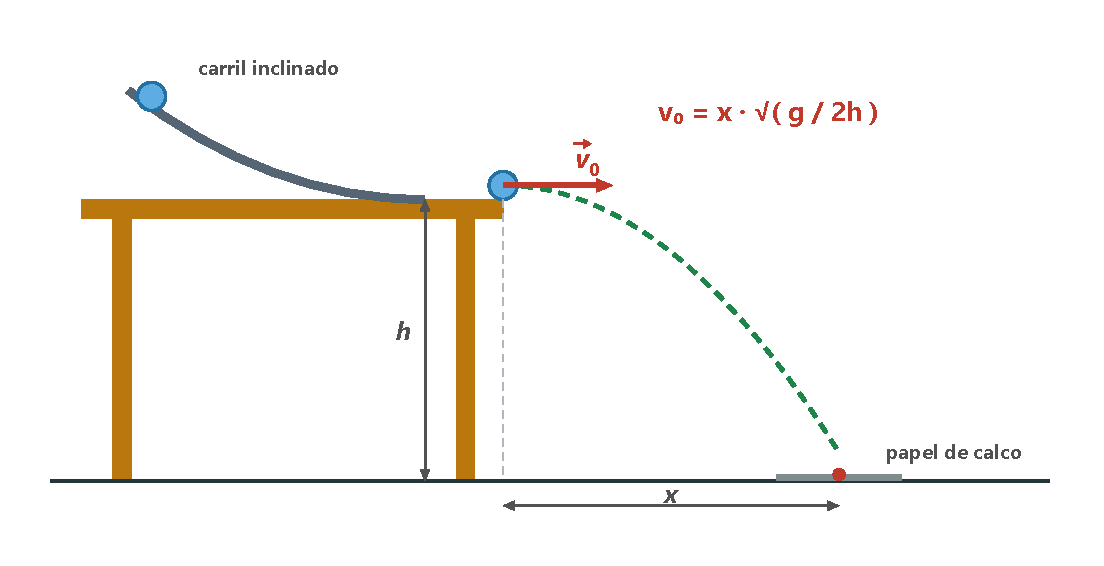
\includegraphics[width=0.7\textwidth]{images/UD9/mesa_rampa}
    \caption{La canica sale de la mesa con velocidad horizontal y cae describiendo media parábola.}
    \label{fig:ud9-mesa}
\end{figure}

\textbf{Procedimiento}
\begin{enumerate}[label=\numberballgreen]
    \item Coloca la rampa sobre la mesa de modo que la canica salga por el borde con velocidad horizontal. Mide la altura \(h\) de la
    mesa.
    \item Pega en el suelo una hoja de papel blanco con papel de calco encima, donde caiga la canica: cada impacto deja una marca.
    \item Suelta la canica siempre desde el mismo punto de la rampa, unas diez veces, y mide la distancia \(x\) desde la vertical del
    borde de la mesa hasta el centro de las marcas.
    \item Repite la experiencia soltándola desde otras alturas de la rampa.
\end{enumerate}

\begin{exercise}
    a) Demuestra que la velocidad con la que la canica sale de la mesa es \(v_0 = x\sqrt{\dfrac{g}{2h}}\). b) Con una mesa de
    \qty{80}{\cm} de altura, la canica cae a \qty{48}{\cm} del borde. Calcula el tiempo de caída y la velocidad de salida. c) ¿Qué
    ocurre con el alcance si la canica sale con el doble de velocidad? ¿Y con el tiempo de caída?
    \begin{solu}
        a) \textcolor{blue}{Tiempo de caída: \(h = \frac{1}{2}\,g\,t^2 \Rightarrow t = \sqrt{2h/g}\); avance horizontal: \(x = v_0\,t\).}
        Despejando, \(\textcolor{red}{v_0 = x/t = x\sqrt{g/(2h)}}\). b) \(t = \sqrt{\num{1.6}/\num{9.8}} = \textcolor{red}{\qty{0.404}{\s}}\);
        \(v_0 = \dfrac{\num{0.48}}{\num{0.404}} = \textcolor{red}{\qty{1.19}{\m\per\s}}\). c) \textcolor{red}{El alcance se duplica,
        pero el tiempo de caída no cambia}: solo depende de la altura.
    \end{solu}
\end{exercise}

%========================================================================================
\section{Situación de aprendizaje: velocidad, seguridad y clima (ODS 13)}\label{sec:ud9-ods}
%========================================================================================

Los vehículos de combustión son una de las principales fuentes de los gases de efecto invernadero y de la contaminación del aire en
las ciudades. Por eso muchas ciudades han creado \textbf{zonas de bajas emisiones}, en las que solo pueden circular los vehículos con
ciertos \textbf{distintivos ambientales} de la DGT (0, ECO, C y B, según sus emisiones), y han reducido los límites de velocidad: la
mayoría de las calles urbanas de un solo carril por sentido están limitadas a \qty{30}{\km\per\hour} desde 2021, y hay calles
escolares limitadas a \qty{20}{\km\per\hour}. El \textbf{ODS 13} (acción por el clima) pide adoptar medidas urgentes para combatir el
cambio climático y sus efectos.

Reducir la velocidad tiene además otra ventaja que podemos calcular con la cinemática: la \textbf{distancia de detención}. Cuando un
conductor ve un peligro, tarda un tiempo en reaccionar (alrededor de \qty{1}{\s}) durante el que el coche sigue a la misma velocidad
(MRU), y después frena (MRUA).

\begin{marker}
    \textbf{Reto:} preparad por grupos un informe sobre las medidas de movilidad y clima de vuestra localidad, con cálculos que
    muestren por qué se limita la velocidad en las ciudades.
\end{marker}

\begin{enumerate}[label=\numberballred]
    \item \textbf{Investigad.} ¿Qué medidas ha tomado vuestro ayuntamiento para reducir la contaminación del tráfico? ¿Qué significa
    cada distintivo ambiental y dónde se exige?
    \item \textbf{Calculad} la distancia de detención de un coche a 20, 30, 50 y \qty{70}{\km\per\hour}, con un tiempo de reacción de
    \qty{1}{\s} y una aceleración de frenado de \qty{-7}{\m\per\s\squared}. Representadla frente a la velocidad.
    \item \textbf{Comparad} los coches de combustión, los eléctricos de batería y los de pila de combustible de hidrógeno: cuatro
    semejanzas y cuatro diferencias (energía que usan, emisiones, autonomía, precio, infraestructura de recarga).
    \item \textbf{Comunicad} vuestras conclusiones con cinco acciones por el clima relacionadas con el transporte que podáis llevar a
    cabo vosotros mismos.
\end{enumerate}

\begin{exercise}
    Resuelve el apartado 2 de la situación de aprendizaje. ¿Por cuánto se multiplica la distancia de detención al pasar de 30 a
    \qty{50}{\km\per\hour}?
    \begin{solu}
        \textcolor{blue}{\(d = v\,t_r + \dfrac{v^2}{2 \cdot 7}\), con \(v\) en m/s.} \textcolor{red}{A \qty{20}{\km\per\hour}
        (\qty{5.56}{\m\per\s}): \(\num{5.6} + \num{2.2} = \qty{7.8}{\m}\); a 30 (\num{8.33}): \(\num{8.3} + \num{5.0} =
        \qty{13.3}{\m}\); a 50 (\num{13.9}): \(\num{13.9} + \num{13.8} = \qty{27.7}{\m}\); a 70 (\num{19.4}): \(\num{19.4} +
        \num{27.0} = \qty{46.4}{\m}\).} La distancia \textcolor{red}{se multiplica por más de 2} (\(\num{27.7}/\num{13.3} =
        \num{2.1}\)): la parte de frenado crece con el cuadrado de la velocidad.
    \end{solu}
\end{exercise}

    \newpage
    %! Unidad 9 — Cinemática aplicada: ejercicios resueltos, ejercicios finales, olimpiadas y autoevaluación
%! Fuente: Fuentes/Fisica/Unidad 9 («Ejercicios resueltos», «Practica y calcula», «Piensa y resuelve») y Unidad 10
%! (captura 217: «Olimpiadas Física» y «Autoevaluación» de este tema). Enunciados adaptados con datos cambiados (y más realistas
%! cuando los de la fuente no lo eran); soluciones rehechas con g = 9,8 m/s². Dificultad: \(\star\) baja, \(\star\star\) media,
%! \(\star\star\star\) alta.

\section{Ejercicios resueltos}\label{sec:ud9-resueltos}

\begin{example}
    \textbf{MRU y MRUA: una persecución.} Mientras estás en una tienda, una persona coge tu bicicleta y empieza a pedalear desde el
    reposo con una aceleración de \qty{1.5}{\m\per\s\squared}. Un coche de policía pasa por delante de la tienda \qty{4}{\s} después,
    a \qty{54}{\km\per\hour} constantes, en la misma dirección. Calcula: a) cuánto tarda la policía en alcanzar a la persona;
    b) a qué distancia de la tienda la alcanza.

    \textbf{Solución.} \textbf{1. Datos}: fugitivo, MRUA con \(v_0 = 0\) y \(a = \qty{1.5}{\m\per\s\squared}\); policía, MRU con
    \(v = \qty{15}{\m\per\s}\) que empieza en la tienda en \(t_0 = \qty{4}{\s}\). Origen en la tienda y \(t = 0\) cuando arranca la bici.

    \textbf{2. Ecuaciones}: \(x_F = \num{0.75}\,t^2\) y \(x_P = 15\,(t - 4)\).

    \textbf{3. a)} La alcanza cuando \(x_F = x_P\): \(\num{0.75}\,t^2 = 15t - 60 \Rightarrow t^2 - 20t + 80 = 0\), con soluciones
    \(t = \qty{5.53}{\s}\) y \(t = \qty{14.5}{\s}\). La primera es el instante en que la policía la alcanza (la segunda sería
    cuando la bicicleta, cada vez más rápida, volvería a adelantar al coche si este no se detuviera).
    \textbf{b)} \(x = \num{0.75} \cdot \num{5.53}^2 = \qty{22.9}{\m}\). Comprobación: \(x_P = 15 \cdot \num{1.53} = \qty{22.9}{\m}\).
\end{example}

\begin{example}
    \textbf{Tiro parabólico: un balón.} Una futbolista golpea un balón desde el suelo a \qty{72}{\km\per\hour} con un ángulo de
    \(35^\circ\) con la horizontal. Determina: a) la altura máxima; b) el tiempo que el balón está en el aire; c) su alcance.

    \textbf{Solución.} \textbf{1. Datos}: \(v_0 = \qty{20}{\m\per\s}\), \(\alpha = 35^\circ\): \(v_{0x} = 20\cos 35^\circ =
    \qty{16.4}{\m\per\s}\); \(v_{0y} = 20\,\sen 35^\circ = \qty{11.5}{\m\per\s}\). \textbf{Incógnitas}: \(y_{\text{máx}}\),
    \(t_{\text{vuelo}}\) y \(x_{\text{máx}}\).

    \textbf{2. a)} En el punto más alto, \(v_y = 0\): \(t = \dfrac{\num{11.47}}{\num{9.8}} = \qty{1.17}{\s}\);
    \(y_{\text{máx}} = \num{11.47} \cdot \num{1.17} - \num{4.9} \cdot \num{1.17}^2 = \qty{6.71}{\m}\).

    \textbf{3. b)} Como sale y llega al mismo nivel, tarda lo mismo en bajar que en subir: \(t_{\text{vuelo}} = \qty{2.34}{\s}\).
    (Comprobación: la caída libre desde \qty{6.71}{\m} dura \(\sqrt{\num{6.71}/\num{4.9}} = \qty{1.17}{\s}\).)

    \textbf{4. c)} \(x_{\text{máx}} = \num{16.38} \cdot \num{2.34} = \qty{38.4}{\m}\).
\end{example}

\begin{example}
    \textbf{MCUA: una rueda.} Una rueda empieza a girar con una aceleración angular de \qty{4}{\radian\per\s\squared} desde una
    posición angular inicial de \(45^\circ\). Calcula: a) las ecuaciones de la posición angular y de la velocidad angular; b) el
    desplazamiento angular y la velocidad angular \qty{6}{\s} después de empezar a girar.

    \textbf{Solución.} \textbf{1. Datos}: \(\alpha = \qty{4}{\radian\per\s\squared}\), \(\omega_0 = 0\), \(\varphi_0 = 45^\circ =
    \pi/4~\unit{\radian}\).

    \textbf{2. a)} \(\varphi = \dfrac{\pi}{4} + \dfrac{1}{2} \cdot 4\,t^2 = \dfrac{\pi}{4} + 2t^2\) (rad); \(\omega = 4t\) (rad/s).

    \textbf{3. b)} \(\Delta\varphi = \varphi - \varphi_0 = 2 \cdot 6^2 = \qty{72}{\radian} = \dfrac{72}{2\pi} = \num{11.5}\) vueltas;
    \(\omega(6) = \qty{24}{\radian\per\s}\).
\end{example}

\begin{example}
    \textbf{Tiro parabólico: una bomba volcánica.} Los volcanes en erupción lanzan fragmentos de lava incandescente, las bombas
    volcánicas. En la erupción de 2021 en La Palma, imagina que una bomba sale de la boca de un cono a \qty{1100}{\m} sobre el nivel
    del mar con un ángulo de \(50^\circ\) y destruye un muro situado a \qty{700}{\m} de distancia horizontal y a \qty{600}{\m} de
    altitud. Calcula: a) la velocidad de lanzamiento; b) el tiempo de vuelo hasta el muro.

    \textbf{Solución.} \textbf{1. Datos}: origen al nivel del mar, en la vertical de la boca: \(y_0 = \qty{1100}{\m}\); \(\alpha =
    50^\circ\); punto final \((700, 600)\). \textbf{Incógnitas}: \(v_0\) y \(t\).

    \textbf{2. Ecuaciones}: \(x = v_0\cos 50^\circ\,t\) e \(y = 1100 + v_0\,\sen 50^\circ\,t - \num{4.9}\,t^2\).

    \textbf{3.} Al llegar al muro: \(700 = v_0\cos 50^\circ\,t\) y \(600 = 1100 + v_0\,\sen 50^\circ\,t - \num{4.9}\,t^2\). De la
    primera, \(v_0\,t = \dfrac{700}{\cos 50^\circ}\), y entonces \(v_0\,\sen 50^\circ\,t = 700\,\tg 50^\circ = \qty{834}{\m}\).
    Sustituyendo en la segunda: \(600 = 1100 + 834 - \num{4.9}\,t^2\), de donde \(t = \sqrt{\dfrac{1334}{\num{4.9}}} = \qty{16.5}{\s}\).

    \textbf{4.} \(v_0 = \dfrac{700}{\cos 50^\circ \cdot \num{16.5}} = \qty{66.0}{\m\per\s}\), unos \qty{238}{\km\per\hour}.
\end{example}

\begin{example}
    \textbf{Tiro horizontal: ayuda humanitaria.} Un helicóptero que vuela horizontalmente a \qty{180}{\km\per\hour} y a
    \qty{2000}{\m} de altura suelta un paquete. Calcula: a) el tiempo que tarda el paquete en llegar al suelo; b) a qué distancia
    horizontal del objetivo debe soltarlo; c) dónde está el helicóptero cuando el paquete llega al suelo.

    \textbf{Solución.} El paquete sale con la velocidad del helicóptero, \(v_0 = \qty{50}{\m\per\s}\) horizontal:
    \(x = 50t\), \(y = 2000 - \num{4.9}\,t^2\).
    a) \(y = 0\): \(t = \sqrt{\dfrac{2000}{\num{4.9}}} = \qty{20.2}{\s}\). b) \(x = 50 \cdot \num{20.2} = \qty{1010}{\m}\) antes del
    objetivo. c) Como el paquete avanza en horizontal igual que el helicóptero, este está \textbf{justo en su vertical}, a
    \qty{2000}{\m} de altura (si no se tiene en cuenta el rozamiento con el aire).
\end{example}

%========================================================================================
\section{Ejercicios de aplicación}\label{sec:ud9-aplicacion}
%========================================================================================

\subsection{Movimiento rectilíneo uniforme}

\begin{exercise}
    \(\star\) La luz del Sol tarda 8 minutos y 20 segundos en llegar a la Tierra. ¿A qué distancia está el Sol? (Velocidad de la luz:
    \qty{3e8}{\m\per\s}.)
    \begin{solu}
        \(d = \num{3e8} \cdot 500 = \textcolor{red}{\qty{1.5e11}{\m}}\).
    \end{solu}
\end{exercise}

\begin{exercise}
    \(\star\star\) Una partícula se mueve en línea recta con velocidad constante. Pasa por la posición \qty{40}{\m} en
    \(t = \qty{2}{\s}\) y por la posición \qty{16}{\m} en \(t = \qty{5}{\s}\). a) Representa la gráfica \(x\)-\(t\). b) Calcula su
    velocidad y su posición inicial. c) ¿Qué espacio recorre en \qty{6}{\s}?
    \begin{solu}
        a) Una recta descendente. b) \(v = \dfrac{16 - 40}{5 - 2} = \textcolor{red}{\qty{-8}{\m\per\s}}\);
        \(x_0 = 40 + 8 \cdot 2 = \textcolor{red}{\qty{56}{\m}}\). c) \(\textcolor{red}{\qty{48}{\m}}\).
    \end{solu}
\end{exercise}

\begin{exercise}
    \(\star\) Un móvil parte de la posición \qty{6}{\m} y se desplaza con MRU en sentido positivo a \qty{12}{\m\per\s}. Escribe su
    ecuación de movimiento y dibuja su gráfica \(x\)-\(t\).
    \begin{solu}
        \(\textcolor{red}{x = 6 + 12t}\) (SI): una recta de pendiente 12 que corta al eje vertical en 6.
    \end{solu}
\end{exercise}

\begin{exercise}
    \(\star\star\) Dos amigos viven en dos pueblos separados \qty{18}{\km} y salen a la vez, uno hacia el otro, por una carretera
    recta. Se encuentran a \qty{7.5}{\km} del primer pueblo al cabo de \qty{25}{\minute}. ¿Qué velocidad lleva cada uno?
    \begin{solu}
        \(v_1 = \dfrac{\num{7.5}}{25/60} = \textcolor{red}{\qty{18}{\km\per\hour}}\) (\qty{5}{\m\per\s}); \(v_2 = \dfrac{\num{10.5}}{25/60} =
        \textcolor{red}{\qty{25.2}{\km\per\hour}}\) (\qty{7}{\m\per\s}).
    \end{solu}
\end{exercise}

\begin{exercise}
    \(\star\star\) Un tren con MRU tarda \qty{15}{\s} en pasar por delante de Luis y \qty{40}{\s} desde que su cabeza entra en un
    túnel de \qty{1000}{\m} hasta que su cola sale de él. ¿Qué longitud tiene el tren? ¿A qué velocidad va?
    \begin{solu}
        \textcolor{blue}{\(L = 15\,v\) y \(L + 1000 = 40\,v\).} \(\textcolor{red}{v = \qty{40}{\m\per\s}}\) (\qty{144}{\km\per\hour});
        \(\textcolor{red}{L = \qty{600}{\m}}\).
    \end{solu}
\end{exercise}

\begin{exercise}
    \(\star\star\) En un videojuego, el coche de Carla pasa por un cruce a \qty{20}{\m\per\s} y, \qty{8}{\s} después, pasa por el
    mismo cruce otro coche a \qty{30}{\m\per\s}, en el mismo sentido. Los dos llevan MRU. a) Representa sus posiciones frente al
    tiempo. b) ¿Cuándo y a qué distancia del cruce la adelanta? c) ¿Qué distancia los separa \qty{10}{\s} después del adelantamiento?
    \begin{solu}
        \textcolor{blue}{\(x_C = 20t\); \(x_2 = 30(t - 8)\).} b) \(\textcolor{red}{t = \qty{24}{\s}}\) desde que Carla pasó el cruce, a
        \(\textcolor{red}{\qty{480}{\m}}\). c) \(10 \cdot (30 - 20) = \textcolor{red}{\qty{100}{\m}}\).
    \end{solu}
\end{exercise}

\subsection{Movimiento rectilíneo uniformemente acelerado}

\begin{exercise}
    \(\star\) Un vehículo arranca con una aceleración de \qty{1.2}{\m\per\s\squared}. Calcula su velocidad \qty{8}{\s} después y la
    distancia que ha recorrido.
    \begin{solu}
        \(v = \textcolor{red}{\qty{9.6}{\m\per\s}}\); \(\Delta x = \num{0.6} \cdot 64 = \textcolor{red}{\qty{38.4}{\m}}\).
    \end{solu}
\end{exercise}

\begin{exercise}
    \(\star\) Un coche que circula a \qty{54}{\km\per\hour} acelera a razón de \qty{2}{\m\per\s\squared} durante \qty{10}{\s}.
    ¿Qué velocidad alcanza y qué espacio recorre?
    \begin{solu}
        \(v = 15 + 20 = \textcolor{red}{\qty{35}{\m\per\s}}\); \(\Delta x = 150 + 100 = \textcolor{red}{\qty{250}{\m}}\).
    \end{solu}
\end{exercise}

\begin{exercise}
    \(\star\) Un coche pasa de 0 a \qty{100}{\km\per\hour} en \qty{8}{\s}. Calcula su aceleración media y la distancia que recorre.
    \begin{solu}
        \(a = \dfrac{\num{27.8}}{8} = \textcolor{red}{\qty{3.47}{\m\per\s\squared}}\); \(\Delta x = \dfrac{\num{27.8}}{2} \cdot 8 =
        \textcolor{red}{\qty{111}{\m}}\).
    \end{solu}
\end{exercise}

\begin{exercise}
    \(\star\star\) Un patinete eléctrico circula durante \qty{6}{\minute} a \qty{18}{\km\per\hour} por un carril bici recto y
    después acelera a \qty{0.5}{\m\per\s\squared} durante \qty{10}{\s}. Halla: a) la distancia total recorrida; b) la rapidez media
    en todo el recorrido.
    \begin{solu}
        a) \(1800 + (50 + 25) = \textcolor{red}{\qty{1875}{\m}}\). b) \(\dfrac{1875}{370} = \textcolor{red}{\qty{5.07}{\m\per\s}}\).
    \end{solu}
\end{exercise}

\begin{exercise}
    \(\star\star\) Un coche circula a \qty{108}{\km\per\hour} y frena con una aceleración de \qty{-6}{\m\per\s\squared}. ¿Qué
    distancia necesita para detenerse? ¿Cuánto tarda?
    \begin{solu}
        \(\Delta x = \dfrac{30^2}{2 \cdot 6} = \textcolor{red}{\qty{75}{\m}}\); \(t = \dfrac{30}{6} = \textcolor{red}{\qty{5}{\s}}\).
    \end{solu}
\end{exercise}

\begin{exercise}
    \(\star\) Una conductora que va a \qty{25}{\m\per\s} quiere detenerse en \qty{4}{\s} y tiene \qty{45}{\m} hasta el coche de
    delante. ¿Le basta esa distancia?
    \begin{solu}
        \(\Delta x = \dfrac{25 + 0}{2} \cdot 4 = \qty{50}{\m}\): \textcolor{red}{no le basta}; necesita al menos \qty{50}{\m}.
    \end{solu}
\end{exercise}

\begin{exercise}
    \(\star\star\) Un motorista que viaja con velocidad constante frena durante \qty{8}{\s} y recorre \qty{120}{\m} hasta pararse.
    Determina: a) su velocidad inicial; b) la aceleración de frenado; c) la aceleración que necesitaría para pararse en la mitad de
    distancia.
    \begin{solu}
        a) \(v_0 = \dfrac{2 \cdot 120}{8} = \textcolor{red}{\qty{30}{\m\per\s}}\); b) \(\textcolor{red}{\qty{-3.75}{\m\per\s\squared}}\);
        c) \(a = -\dfrac{900}{2 \cdot 60} = \textcolor{red}{\qty{-7.5}{\m\per\s\squared}}\).
    \end{solu}
\end{exercise}

\begin{exercise}
    \(\star\star\) Javier y Elena montan en bicicleta en la misma dirección y sentido con MRUA. Al empezar, Javier va a
    \qty{6}{\m\per\s} con una aceleración de \qty{1}{\m\per\s\squared}, y Elena, a \qty{3}{\m\per\s} con \qty{2}{\m\per\s\squared}.
    a) ¿A qué distancia del inicio está cada uno a los \qty{4}{\s}? b) ¿Qué distancia los separa a los \qty{10}{\s}? c) ¿Cuándo y
    dónde adelanta Elena a Javier?
    \begin{solu}
        a) \(\textcolor{red}{x_J = \qty{32}{\m}}\); \(\textcolor{red}{x_E = \qty{28}{\m}}\). b) \(130 - 110 = \textcolor{red}{\qty{20}{\m}}\)
        (va delante Elena). c) \(6t + \num{0.5}\,t^2 = 3t + t^2\): \(\textcolor{red}{t = \qty{6}{\s}}\), a \(\textcolor{red}{\qty{54}{\m}}\).
    \end{solu}
\end{exercise}

\begin{exercise}
    \(\star\star\star\) Un meteorito cae hacia la Tierra a \qty{12}{\km\per\s} constantes. Cuando está a \qty{90}{\km} de altura,
    alguien lo detecta y, \qty{4}{\s} después, despega del suelo, en vertical y desde el reposo, un dron interceptor con una
    aceleración de \qty{40}{\m\per\s\squared}. a) ¿Cuánto tarda en interceptarlo? b) ¿A qué altura? c) ¿Qué aceleración necesitaría
    para interceptarlo a \qty{300}{\m} de altura?
    \begin{solu}
        \textcolor{blue}{\(y_M = 90000 - 12000t\); \(y_D = 20(t - 4)^2\); \(t^2 + 592t - 4484 = 0\).} a) \(\textcolor{red}{t = \qty{7.48}{\s}}\)
        (\qty{3.48}{\s} después de despegar). b) \(\textcolor{red}{y = \qty{242}{\m}}\). c) El meteorito llega a \qty{300}{\m} en
        \(t = \qty{7.475}{\s}\): \(a = \dfrac{2 \cdot 300}{\num{3.475}^2} = \textcolor{red}{\qty{49.7}{\m\per\s\squared}}\).
    \end{solu}
\end{exercise}

\subsection{Caída libre y lanzamiento vertical}

\begin{exercise}
    \(\star\) ¿Cuánto tarda en llegar al suelo una maceta que cae desde \qty{20}{\m} de altura? ¿Con qué velocidad llega? Desprecia el
    rozamiento con el aire.
    \begin{solu}
        \(t = \sqrt{20/\num{4.9}} = \textcolor{red}{\qty{2.02}{\s}}\); \(v = \textcolor{red}{\qty{19.8}{\m\per\s}}\) hacia abajo.
    \end{solu}
\end{exercise}

\begin{exercise}
    \(\star\) Se lanza un cuerpo verticalmente hacia arriba a \qty{72}{\km\per\hour}. a) ¿Qué altura alcanza? b) ¿Cuánto tarda en
    volver al punto de lanzamiento?
    \begin{solu}
        a) \(\dfrac{20^2}{\num{19.6}} = \textcolor{red}{\qty{20.4}{\m}}\); b) \(2 \cdot \dfrac{20}{\num{9.8}} = \textcolor{red}{\qty{4.08}{\s}}\).
    \end{solu}
\end{exercise}

\begin{exercise}
    \(\star\) Una saltadora se deja caer desde una plataforma de \qty{10}{\m} a la piscina. ¿Con qué velocidad llega al agua? ¿Cuánto
    tiempo está en el aire?
    \begin{solu}
        \(v = \sqrt{2 \cdot \num{9.8} \cdot 10} = \textcolor{red}{\qty{14}{\m\per\s}}\); \(t = \textcolor{red}{\qty{1.43}{\s}}\).
    \end{solu}
\end{exercise}

\begin{exercise}
    \(\star\star\) La aceleración de la gravedad en la superficie de cierto planeta es la tercera parte de la terrestre. Si un robot
    se deja caer desde \qty{150}{\m}, ¿con qué velocidad llega a la superficie? ¿Cuánto tarda?
    \begin{solu}
        \(g' = \qty{3.27}{\m\per\s\squared}\); \(v = \sqrt{2 \cdot \num{3.27} \cdot 150} = \textcolor{red}{\qty{31.3}{\m\per\s}}\);
        \(t = \sqrt{300/\num{3.27}} = \textcolor{red}{\qty{9.58}{\s}}\).
    \end{solu}
\end{exercise}

\begin{exercise}
    \(\star\star\) Durante el asedio a un castillo medieval, los defensores lanzan piedras hacia abajo a \qty{10}{\m\per\s} desde
    \qty{30}{\m} de altura. Calcula: a) el tiempo que tarda una piedra en llegar al suelo; b) su velocidad después de recorrer
    \qty{15}{\m}; c) el tiempo que tarda en recorrer el último metro y la velocidad que gana en él.
    \begin{solu}
        a) \(\num{4.9}\,t^2 + 10t - 30 = 0\): \(\textcolor{red}{t = \qty{1.66}{\s}}\). b) \(v = -\sqrt{100 + 2 \cdot \num{9.8} \cdot 15} =
        \textcolor{red}{\qty{-19.8}{\m\per\s}}\). c) \textcolor{blue}{Llega a \qty{1}{\m} del suelo en \(t = \qty{1.618}{\s}\).}
        \(\textcolor{red}{\Delta t = \qty{0.038}{\s}}\); \(\Delta v = \num{9.8} \cdot \num{0.038} = \textcolor{red}{\qty{0.38}{\m\per\s}}\).
    \end{solu}
\end{exercise}

\begin{exercise}
    \(\star\star\) Un tornillo se desprende de un helicóptero que desciende a \qty{8}{\m\per\s} constantes. a) Calcula la velocidad y
    el desplazamiento del tornillo \qty{4}{\s} después. b) Repite el cálculo si el helicóptero asciende a la misma velocidad.
    \begin{solu}
        a) \(v = -8 - \num{39.2} = \textcolor{red}{\qty{-47.2}{\m\per\s}}\); \(\Delta y = -32 - \num{78.4} = \textcolor{red}{\qty{-110.4}{\m}}\).
        b) \(v = 8 - \num{39.2} = \textcolor{red}{\qty{-31.2}{\m\per\s}}\); \(\Delta y = 32 - \num{78.4} = \textcolor{red}{\qty{-46.4}{\m}}\).
    \end{solu}
\end{exercise}

\begin{exercise}
    \(\star\star\) Desde el balcón más alto de la Giralda de Sevilla, a unos \qty{97}{\m} del suelo, se lanza verticalmente hacia
    arriba una rosa a \qty{10}{\m\per\s}. Halla: a) el tiempo hasta la altura máxima y su valor; b) el tiempo que está la rosa en el
    aire y la velocidad con que llega al suelo; c) dibuja las gráficas \(y\)-\(t\), \(v\)-\(t\) y \(a\)-\(t\).
    \begin{solu}
        a) \(\textcolor{red}{t = \qty{1.02}{\s}}\); \(y_{\text{máx}} = 97 + \dfrac{100}{\num{19.6}} = \textcolor{red}{\qty{102.1}{\m}}\).
        b) \(\num{4.9}\,t^2 - 10t - 97 = 0\): \(\textcolor{red}{t = \qty{5.59}{\s}}\); \(v = 10 - \num{9.8} \cdot \num{5.59} =
        \textcolor{red}{\qty{-44.7}{\m\per\s}}\). c) \textcolor{red}{Una parábola cóncava hacia abajo, una recta decreciente y una
        recta horizontal en \(-g\)}.
    \end{solu}
\end{exercise}

\begin{exercise}
    \(\star\star\) Se lanzan verticalmente hacia arriba, desde el mismo punto y con \qty{0.5}{\s} de diferencia, dos pelotas: la
    primera a \qty{5}{\m\per\s} y la segunda a \qty{7}{\m\per\s}. Determina: a) cuándo se cruzan; b) la altura del cruce; c) la
    velocidad de cada pelota en ese instante.
    \begin{solu}
        \textcolor{blue}{\(5t - \num{4.9}\,t^2 = 7(t - \num{0.5}) - \num{4.9}(t - \num{0.5})^2\).} a) \(\textcolor{red}{t = \qty{0.685}{\s}}\)
        tras lanzar la primera. b) \(\textcolor{red}{y = \qty{1.13}{\m}}\). c) \(\textcolor{red}{v_1 = \qty{-1.71}{\m\per\s}}\) (baja) y
        \(\textcolor{red}{v_2 = \qty{5.19}{\m\per\s}}\) (sube).
    \end{solu}
\end{exercise}

\begin{exercise}
    \(\star\star\) Desde \qty{150}{\m} de altura se lanza una moneda hacia arriba a \qty{15}{\m\per\s}. \qty{2}{\s} después se deja
    caer otra desde el mismo punto. a) ¿Cuánto tardan en encontrarse? b) ¿Qué velocidad tiene cada una en el cruce? c) ¿A qué altura
    se cruzan?
    \begin{solu}
        \textcolor{blue}{\(150 + 15t - \num{4.9}\,t^2 = 150 - \num{4.9}(t - 2)^2 \Rightarrow \num{4.6}\,t = \num{19.6}\).}
        a) \(\textcolor{red}{t = \qty{4.26}{\s}}\) tras lanzar la primera. b) \(\textcolor{red}{v_1 = \qty{-26.8}{\m\per\s}}\);
        \(\textcolor{red}{v_2 = \qty{-22.2}{\m\per\s}}\). c) \(\textcolor{red}{y = \qty{125}{\m}}\).
    \end{solu}
\end{exercise}

\subsection{Composición de movimientos}

\begin{exercise}
    \(\star\) Un barco cruza un río de \qty{90}{\m} de ancho a \qty{6}{\m\per\s}, perpendicularmente a una corriente de
    \qty{2.5}{\m\per\s}. ¿Cuánto tarda y a qué distancia río abajo llega a la otra orilla?
    \begin{solu}
        \(t = \dfrac{90}{6} = \textcolor{red}{\qty{15}{\s}}\); \(x = \num{2.5} \cdot 15 = \textcolor{red}{\qty{37.5}{\m}}\).
    \end{solu}
\end{exercise}

\begin{exercise}
    \(\star\star\) Pedro quiere cruzar un río de \qty{2}{\km} de ancho en una barca que avanza a \qty{30}{\km\per\hour} respecto al
    agua, perpendicularmente a la orilla. La corriente es de \qty{6}{\km\per\hour}. Calcula: a) la velocidad de la barca respecto a la
    orilla; b) el tiempo que tarda en cruzar; c) la distancia que recorre río abajo.
    \begin{solu}
        a) \(\sqrt{900 + 36} = \textcolor{red}{\qty{30.6}{\km\per\hour}}\); b) \(\dfrac{2}{30}~\unit{\hour} = \textcolor{red}{\qty{4}{\minute}}\);
        c) \(6 \cdot \dfrac{2}{30} = \textcolor{red}{\qty{0.4}{\km}}\).
    \end{solu}
\end{exercise}

\begin{exercise}
    \(\star\star\) Una persona rema en una canoa a \qty{2.5}{\m\per\s} respecto al agua, formando un ángulo de \(60^\circ\) con la
    dirección de la corriente (río abajo), para cruzar un río de \qty{50}{\m} de ancho cuya corriente es de \qty{1.5}{\m\per\s}.
    a) Escribe el vector velocidad de la canoa respecto a la orilla y su vector posición en función del tiempo. b) ¿Cuánto tarda en
    cruzar y qué distancia recorre río abajo?
    \begin{solu}
        a) \(\vec v = (\num{2.5}\cos 60^\circ + \num{1.5})\,\ivec + \num{2.5}\,\sen 60^\circ\,\jvec =
        \textcolor{red}{(\num{2.75}\,\ivec + \num{2.17}\,\jvec)~\unit{\m\per\s}}\); \(\textcolor{red}{\vec r = \num{2.75}\,t\,\ivec +
        \num{2.17}\,t\,\jvec}\). b) \(t = \dfrac{50}{\num{2.165}} = \textcolor{red}{\qty{23.1}{\s}}\); \(x = \textcolor{red}{\qty{63.5}{\m}}\).
    \end{solu}
\end{exercise}

\begin{exercise}
    \(\star\) En un aeropuerto, una cinta transportadora de \qty{50}{\m} avanza a \qty{0.8}{\m\per\s}. Calcula cuánto tarda en
    recorrerla una persona: a) quieta sobre la cinta; b) andando a \qty{1.2}{\m\per\s} en el sentido de la cinta; c) andando en sentido
    contrario.
    \begin{solu}
        a) \(\dfrac{50}{\num{0.8}} = \textcolor{red}{\qty{62.5}{\s}}\); b) \(\dfrac{50}{2} = \textcolor{red}{\qty{25}{\s}}\);
        c) \(\dfrac{50}{\num{0.4}} = \textcolor{red}{\qty{125}{\s}}\) (avanza al revés que la cinta).
    \end{solu}
\end{exercise}

\subsection{Tiro horizontal}

\begin{exercise}
    \(\star\) Desde una ventana a \qty{8}{\m} de altura sale horizontalmente el agua de una manguera a \qty{10}{\m\per\s}. ¿A qué
    distancia de la pared cae el agua?
    \begin{solu}
        \(t = \sqrt{8/\num{4.9}} = \qty{1.28}{\s}\); \(x = \textcolor{red}{\qty{12.8}{\m}}\).
    \end{solu}
\end{exercise}

\begin{exercise}
    \(\star\) Una pelota sale rodando por el borde de una mesa de \qty{80}{\cm} de altura a \qty{1.5}{\m\per\s}. ¿Cuánto tarda en
    llegar al suelo? ¿Con qué velocidad lo hace? ¿A qué distancia de la mesa cae?
    \begin{solu}
        \(\textcolor{red}{t = \qty{0.404}{\s}}\); \(\textcolor{red}{\vec v = (\num{1.5}\,\ivec - \num{3.96}\,\jvec)~\unit{\m\per\s}}\);
        \(x = \textcolor{red}{\qty{0.61}{\m}}\).
    \end{solu}
\end{exercise}

\begin{exercise}
    \(\star\star\) Javier sube a la azotea de un edificio de \qty{15}{\m} y lanza un balón horizontalmente a \qty{18}{\m\per\s}.
    Despreciando el rozamiento, calcula: a) la distancia al edificio a la que cae; b) el tiempo que tarda; c) su velocidad al llegar
    al suelo.
    \begin{solu}
        a) \(\textcolor{red}{\qty{31.5}{\m}}\); b) \(\textcolor{red}{\qty{1.75}{\s}}\); c) \(\textcolor{red}{\vec v = (18\,\ivec -
        \num{17.1}\,\jvec)~\unit{\m\per\s}}\), de módulo \qty{24.8}{\m\per\s}.
    \end{solu}
\end{exercise}

\begin{exercise}
    \(\star\star\) Desde la cumbre del Mulhacén, Nieves lanza un plato volador horizontalmente a \qty{50}{\m\per\s} hacia un valle
    situado \qty{1000}{\m} más abajo. Suponiendo que nada lo frena, determina: a) cuánto tarda en llegar al valle; b) a qué
    distancia horizontal cae; c) su velocidad y su posición, respecto al punto de lanzamiento, a los \qty{10}{\s}.
    \begin{solu}
        a) \(t = \sqrt{1000/\num{4.9}} = \textcolor{red}{\qty{14.3}{\s}}\); b) \(\textcolor{red}{\qty{714}{\m}}\);
        c) \(\textcolor{red}{\vec v = (50\,\ivec - 98\,\jvec)~\unit{\m\per\s}}\); \(\textcolor{red}{\vec r = (500\,\ivec - 490\,\jvec)~\unit{\m}}\).
    \end{solu}
\end{exercise}

\begin{exercise}
    \(\star\star\) Desde un helicóptero parado a \qty{45}{\m} sobre el mar, un socorrista se lanza horizontalmente a
    \qty{8}{\m\per\s} para rescatar a una persona. Calcula: a) a qué distancia del helicóptero (en horizontal) cae al agua; b) el
    tiempo que está en el aire; c) su velocidad al llegar al agua.
    \begin{solu}
        a) \(\textcolor{red}{\qty{24.2}{\m}}\); b) \(\textcolor{red}{\qty{3.03}{\s}}\); c) \(\textcolor{red}{\vec v = (8\,\ivec -
        \num{29.7}\,\jvec)~\unit{\m\per\s}}\).
    \end{solu}
\end{exercise}

\begin{exercise}
    \(\star\star\) Un avión vuela horizontalmente a \qty{800}{\m} de altura y a \qty{360}{\km\per\hour} y suelta un paquete.
    Determina: a) el tiempo que tarda en llegar al suelo; b) la distancia horizontal que recorre; c) a qué distancia del avión está el
    paquete cuando toca el suelo, si el avión sigue igual.
    \begin{solu}
        a) \(\textcolor{red}{\qty{12.8}{\s}}\); b) \(\textcolor{red}{\qty{1278}{\m}}\); c) \textcolor{red}{A \qty{800}{\m}, justo
        debajo}: los dos avanzan lo mismo en horizontal.
    \end{solu}
\end{exercise}

\subsection{Tiro parabólico}

\begin{exercise}
    \(\star\star\) Jorge salta con una moto de agua que va a \qty{54}{\km\per\hour} por una ola que le hace despegar con un ángulo de
    \(15^\circ\). Calcula: a) la distancia que recorre en el aire; b) el tiempo que está en el aire; c) la posición del punto más alto.
    \begin{solu}
        a) \(\dfrac{225\,\sen 30^\circ}{\num{9.8}} = \textcolor{red}{\qty{11.5}{\m}}\); b) \(\textcolor{red}{\qty{0.79}{\s}}\);
        c) \(\textcolor{red}{(\num{5.74}; \num{0.77})~\unit{\m}}\).
    \end{solu}
\end{exercise}

\begin{exercise}
    \(\star\star\) Desde la azotea de un chalet, a \qty{15}{\m} de altura, se lanza un globo de agua a \qty{25}{\m\per\s} con un
    ángulo de \(30^\circ\) sobre la horizontal. Determina: a) a qué distancia de la base de la casa cae; b) el tiempo que está en el
    aire; c) su velocidad al llegar al suelo; d) su vector posición en \(t = \qty{1}{\s}\).
    \begin{solu}
        \textcolor{blue}{\(x = \num{21.65}\,t\); \(y = 15 + \num{12.5}\,t - \num{4.9}\,t^2\).} b) \(\textcolor{red}{t = \qty{3.44}{\s}}\);
        a) \(\textcolor{red}{x = \qty{74.5}{\m}}\); c) \(\textcolor{red}{\vec v = (\num{21.7}\,\ivec - \num{21.2}\,\jvec)~\unit{\m\per\s}}\),
        de módulo \qty{30.3}{\m\per\s}; d) \(\textcolor{red}{\vec r = (\num{21.7}\,\ivec + \num{22.6}\,\jvec)~\unit{\m}}\).
    \end{solu}
\end{exercise}

\begin{exercise}
    \(\star\star\) Una atleta de triple salto se pregunta qué velocidad necesita en un salto con un ángulo de \(30^\circ\) para
    recorrer \qty{14}{\m} (considera el salto como un tiro parabólico de su centro de masas).
    \begin{solu}
        \(14 = \dfrac{v_0^2\,\sen 60^\circ}{\num{9.8}}\): \(\textcolor{red}{v_0 = \qty{12.6}{\m\per\s}}\).
    \end{solu}
\end{exercise}

\begin{exercise}
    \(\star\star\) Un jugador de baloncesto lanza a canasta desde \qty{7}{\m} de distancia horizontal, a \qty{8.8}{\m\per\s} y con un
    ángulo de \(45^\circ\). El balón sale a \qty{2.1}{\m} del suelo y el aro está a \qty{3.05}{\m}. ¿A qué altura pasa el balón por la
    vertical del aro? ¿Encestará?
    \begin{solu}
        \textcolor{blue}{\(v_{0x} = \qty{6.22}{\m\per\s}\); llega a \(x = 7\) en \(t = \qty{1.12}{\s}\).} \(y = \num{2.1} + \num{6.22} \cdot
        \num{1.12} - \num{4.9} \cdot \num{1.12}^2 = \textcolor{red}{\qty{2.90}{\m}}\): \textcolor{red}{se queda corto}, pasa
        \qty{15}{\cm} por debajo del aro.
    \end{solu}
\end{exercise}

\begin{exercise}
    \(\star\star\star\) Un atleta lanza la jabalina desde \qty{2}{\m} de altura a \qty{28}{\m\per\s}. ¿Con qué ángulo debe lanzarla
    para que caiga a \qty{60}{\m}? (Usa \(\dfrac{1}{\cos^2\alpha} = 1 + \tg^2\alpha\).)
    \begin{solu}
        \textcolor{blue}{Ecuación de la trayectoria con \(y = 0\), \(x = 60\): \(0 = 2 + 60\,\tg\alpha - \num{22.5}(1 + \tg^2\alpha)\),
        es decir, \(\num{22.5}\,\tg^2\alpha - 60\,\tg\alpha + \num{20.5} = 0\).} \(\tg\alpha = \num{2.26}\) o \num{0.402}:
        \(\textcolor{red}{\alpha = 66.2^\circ}\) o \(\textcolor{red}{\alpha = 21.9^\circ}\).
    \end{solu}
\end{exercise}

\begin{exercise}
    \(\star\star\star\) María vive en un cuarto piso (cada piso mide \qty{2.8}{\m}) y lanza con un tirachinas una caja pequeña a
    \qty{20}{\m\per\s} con un ángulo de \(45^\circ\) \textbf{por debajo} de la horizontal hacia Pilar, que está en la calle.
    Determina: a) a qué distancia del edificio debe colocarse Pilar; b) el tiempo que la caja está en el aire y su velocidad al
    llegar al suelo.
    \begin{solu}
        \textcolor{blue}{\(y_0 = \qty{11.2}{\m}\); \(v_{0x} = \qty{14.1}{\m\per\s}\); \(v_{0y} = \qty{-14.1}{\m\per\s}\);
        \(\num{4.9}\,t^2 + \num{14.14}\,t - \num{11.2} = 0\).} b) \(\textcolor{red}{t = \qty{0.65}{\s}}\);
        \(\textcolor{red}{\vec v = (\num{14.1}\,\ivec - \num{20.5}\,\jvec)~\unit{\m\per\s}}\). a) \(x = \textcolor{red}{\qty{9.1}{\m}}\).
    \end{solu}
\end{exercise}

\subsection{Movimiento circular uniforme}

\begin{exercise}
    \(\star\) Una partícula describe una circunferencia de \qty{40}{\cm} de radio a \qty{30}{rpm}. Expresa su periodo, su frecuencia,
    su velocidad angular y su velocidad lineal en el SI.
    \begin{solu}
        \(\textcolor{red}{T = \qty{2}{\s}}\); \(\textcolor{red}{f = \qty{0.5}{\hertz}}\); \(\textcolor{red}{\omega = \pi = \qty{3.14}{\radian\per\s}}\);
        \(\textcolor{red}{v = \qty{1.26}{\m\per\s}}\).
    \end{solu}
\end{exercise}

\begin{exercise}
    \(\star\) Una lavadora centrifuga a \qty{1000}{rpm} y su tambor tiene \qty{50}{\cm} de diámetro. Calcula la velocidad angular, la
    velocidad lineal de la ropa pegada al tambor, el periodo y la frecuencia.
    \begin{solu}
        \(\textcolor{red}{\omega = \qty{105}{\radian\per\s}}\); \(\textcolor{red}{v = \qty{26.2}{\m\per\s}}\); \(\textcolor{red}{T = \qty{0.06}{\s}}\);
        \(\textcolor{red}{f = \qty{16.7}{\hertz}}\).
    \end{solu}
\end{exercise}

\begin{exercise}
    \(\star\) El volante de un triciclo, de \qty{40}{\cm} de diámetro, da 6 vueltas por minuto. Calcula su velocidad angular, la
    velocidad lineal de un punto del borde y su aceleración normal.
    \begin{solu}
        \(\textcolor{red}{\omega = \qty{0.628}{\radian\per\s}}\); \(\textcolor{red}{v = \qty{0.126}{\m\per\s}}\);
        \(\textcolor{red}{a_n = \qty{0.079}{\m\per\s\squared}}\).
    \end{solu}
\end{exercise}

\begin{exercise}
    \(\star\star\) Una mosca se posa en el extremo del aspa de un ventilador de \qty{60}{\cm} de diámetro que gira a \qty{90}{rpm}.
    Determina: a) su velocidad angular y lineal; b) su periodo y su frecuencia; c) su aceleración normal; d) el ángulo y el arco que
    recorre en \qty{2}{\s}.
    \begin{solu}
        a) \(\textcolor{red}{\qty{9.42}{\radian\per\s}}\) y \(\textcolor{red}{\qty{2.83}{\m\per\s}}\); b) \(\textcolor{red}{\qty{0.667}{\s}}\) y
        \(\textcolor{red}{\qty{1.5}{\hertz}}\); c) \(\textcolor{red}{\qty{26.6}{\m\per\s\squared}}\); d) \(\textcolor{red}{\qty{18.8}{\radian}}\)
        y \(\textcolor{red}{\qty{5.65}{\m}}\).
    \end{solu}
\end{exercise}

\begin{exercise}
    \(\star\star\) ¿Cuál es la velocidad angular de cada una de las agujas de un reloj analógico?
    \begin{solu}
        Horaria (una vuelta en \qty{12}{\hour}): \(\textcolor{red}{\qty{1.45e-4}{\radian\per\s}}\); minutero (\qty{1}{\hour}):
        \(\textcolor{red}{\qty{1.75e-3}{\radian\per\s}}\); segundero (\qty{1}{\minute}): \(\textcolor{red}{\qty{0.105}{\radian\per\s}}\).
    \end{solu}
\end{exercise}

\begin{exercise}
    \(\star\star\star\) La Estación Espacial Internacional (ISS) da una vuelta a la Tierra cada \qty{92}{\minute} en una órbita
    prácticamente circular a unos \qty{410}{\km} de altura. Si el radio de la Tierra es de \qty{6370}{\km}, calcula: a) su velocidad
    angular, su periodo y su frecuencia; b) su velocidad lineal; c) su aceleración normal.
    \begin{solu}
        \textcolor{blue}{\(R = \qty{6.78e6}{\m}\); \(T = \qty{5520}{\s}\).} a) \(\textcolor{red}{\omega = \qty{1.14e-3}{\radian\per\s}}\);
        \(\textcolor{red}{f = \qty{1.81e-4}{\hertz}}\). b) \(\textcolor{red}{v = \qty{7.72e3}{\m\per\s}}\) (casi \qty{28000}{\km\per\hour}).
        c) \(\textcolor{red}{a_n = \qty{8.78}{\m\per\s\squared}}\): casi la misma \(g\) que en la superficie.
    \end{solu}
\end{exercise}

\subsection{Movimiento circular uniformemente acelerado}

\begin{exercise}
    \(\star\) Una rueda de un tractor alcanza las 60 vueltas por minuto \qty{15}{\s} después de arrancar desde el reposo. Calcula su
    aceleración angular, el ángulo que describe en esos \qty{15}{\s} y las vueltas que da.
    \begin{solu}
        \(\textcolor{red}{\alpha = \qty{0.419}{\radian\per\s\squared}}\); \(\textcolor{red}{\Delta\varphi = \qty{47.1}{\radian}}\);
        \(\textcolor{red}{\num{7.5}~\text{vueltas}}\).
    \end{solu}
\end{exercise}

\begin{exercise}
    \(\star\star\) Al levantar la aguja de un tocadiscos, el disco, de \qty{30}{\cm} de diámetro, que giraba a \qty{45}{rpm}, se
    detiene en \qty{12}{\s}. Determina: a) la aceleración angular y la velocidad lineal de un punto del borde a los \qty{4}{\s};
    b) las vueltas que da hasta pararse.
    \begin{solu}
        a) \(\textcolor{red}{\alpha = \qty{-0.393}{\radian\per\s\squared}}\); \(\omega(4) = \qty{3.14}{\radian\per\s}\) y
        \(\textcolor{red}{v = \qty{0.47}{\m\per\s}}\). b) \(\Delta\varphi = \qty{28.3}{\radian}\): \(\textcolor{red}{\num{4.5}~\text{vueltas}}\).
    \end{solu}
\end{exercise}

\begin{exercise}
    \(\star\star\) El volante de un coche de carreras gira desde el reposo con una aceleración angular de \qty{2}{\radian\per\s\squared}.
    a) ¿Cuánto tarda en girar \(90^\circ\)? b) ¿Qué velocidad angular tiene entonces?
    \begin{solu}
        a) \(\dfrac{\pi}{2} = t^2\): \(\textcolor{red}{t = \qty{1.25}{\s}}\). b) \(\textcolor{red}{\omega = \qty{2.51}{\radian\per\s}}\).
    \end{solu}
\end{exercise}

\begin{exercise}
    \(\star\star\) Una motocicleta da vueltas a un circuito circular de \qty{150}{\m} de diámetro. Parte del reposo con MCUA y,
    \qty{25}{\s} después, circula a \qty{54}{\km\per\hour}; a partir de ahí sigue con MCU. a) Calcula sus aceleraciones tangencial,
    normal, total y angular justo antes de llegar a los \qty{25}{\s}. b) ¿Qué velocidad angular alcanza? ¿Cuál es entonces su
    periodo?
    \begin{solu}
        a) \(\textcolor{red}{a_t = \qty{0.6}{\m\per\s\squared}}\); \(\textcolor{red}{a_n = \dfrac{225}{75} = \qty{3}{\m\per\s\squared}}\);
        \(\textcolor{red}{a = \qty{3.06}{\m\per\s\squared}}\); \(\textcolor{red}{\alpha = \qty{0.008}{\radian\per\s\squared}}\).
        b) \(\textcolor{red}{\omega = \qty{0.2}{\radian\per\s}}\); \(\textcolor{red}{T = \qty{31.4}{\s}}\).
    \end{solu}
\end{exercise}

\begin{exercise}
    \(\star\star\) Un engranaje gira a \qty{20}{\radian\per\s} y frena con una aceleración angular de \qty{-4}{\radian\per\s\squared}.
    Calcula el tiempo que tarda en detenerse y el ángulo que recorre.
    \begin{solu}
        \(\textcolor{red}{t = \qty{5}{\s}}\); \(\Delta\varphi = \dfrac{20}{2} \cdot 5 = \textcolor{red}{\qty{50}{\radian}}\).
    \end{solu}
\end{exercise}

%========================================================================================
\section{Ejercicios de ampliación}\label{sec:ud9-ampliacion}
%========================================================================================

\begin{exercise}
    \(\star\star\) Esta tabla recoge la velocidad de un coche durante una carrera:
    \begin{center}
        \begin{tabular}{@{}lcccccccc@{}}
            \toprule
            \(\boldsymbol{t}\) \textbf{(s)} & 0 & 5 & 10 & 15 & 20 & 25 & 30 & 35 \\
            \midrule
            \(\boldsymbol{v}\) \textbf{(m/s)} & 4 & 4 & 4 & 12 & 20 & 20 & 20 & 8 \\
            \bottomrule
        \end{tabular}
    \end{center}
    a) Representa la gráfica \(v\)-\(t\). b) Identifica el tipo de movimiento de cada tramo y su aceleración. c) Calcula el espacio
    recorrido en los \qty{35}{\s}.
    \begin{solu}
        b) \textcolor{red}{0-10 s: MRU (\(a = 0\)); 10-20 s: MRUA (\(a = \qty{1.6}{\m\per\s\squared}\)); 20-30 s: MRU; 30-35 s: MRUA de
        frenado (\(a = \qty{-2.4}{\m\per\s\squared}\))}. c) Área bajo la gráfica: \(40 + 120 + 200 + 70 = \textcolor{red}{\qty{430}{\m}}\).
    \end{solu}
\end{exercise}

\begin{exercise}
    \(\star\star\) Arantxa entra corriendo en el andén a \qty{4}{\m\per\s} justo cuando su tren arranca con una aceleración de
    \qty{0.5}{\m\per\s\squared}. Entre ella y la puerta del último vagón hay \qty{15}{\m}. ¿Conseguirá subir al tren?
    \begin{solu}
        \textcolor{blue}{\(4t = 15 + \num{0.25}\,t^2 \Rightarrow t^2 - 16t + 60 = 0\).} \textcolor{red}{Sí}: alcanza la puerta a los
        \(\textcolor{red}{\qty{6}{\s}}\), cuando el tren ha avanzado \qty{9}{\m}. (A los 6 s el tren va a \qty{3}{\m\per\s}, más
        despacio que ella.)
    \end{solu}
\end{exercise}

\begin{exercise}
    \(\star\star\star\) La protagonista de una serie huye por un camino que cruza perpendicularmente una vía de tren. Un tren se
    acerca al cruce a \qty{72}{\km\per\hour} y está a \qty{400}{\m} cuando ella, que está parada a \qty{60}{\m} del cruce, empieza a
    correr hacia él con aceleración constante. a) ¿Qué aceleración necesita para llegar al cruce justo cuando llega el tren? b) ¿Con qué
    velocidad llega?
    \begin{solu}
        \textcolor{blue}{El tren llega en \(t = 400/20 = \qty{20}{\s}\).} a) \(60 = \frac{1}{2}\,a \cdot 400\): \(\textcolor{red}{a =
        \qty{0.3}{\m\per\s\squared}}\). b) \(v = \num{0.3} \cdot 20 = \textcolor{red}{\qty{6}{\m\per\s}}\).
    \end{solu}
\end{exercise}

\begin{exercise}
    \(\star\star\) Una maceta cae desde el poyete de una ventana. Manuel ve que pasa por delante de la suya, que está a \qty{8}{\m} del
    suelo, \qty{1.5}{\s} después de caer. ¿A qué altura estaba el poyete?
    \begin{solu}
        \(h = 8 + \num{4.9} \cdot \num{1.5}^2 = \textcolor{red}{\qty{19.0}{\m}}\).
    \end{solu}
\end{exercise}

\begin{exercise}
    \(\star\star\star\) Desde lo alto de un acantilado se deja caer una piedra, que recorre la última cuarta parte de la altura en
    \qty{1}{\s}. ¿Qué altura tiene el acantilado?
    \begin{solu}
        \textcolor{blue}{Si la caída dura \(T\): \(h = \num{4.9}\,T^2\) y \(\frac{3}{4}h = \num{4.9}(T - 1)^2\), así que \(T - 1 =
        \sqrt{3/4}\,T\) y \(T = \qty{7.46}{\s}\).} \(h = \textcolor{red}{\qty{273}{\m}}\).
    \end{solu}
\end{exercise}

\begin{exercise}
    \(\star\star\star\) Un cohete parte del reposo y sube verticalmente con una aceleración de \qty{2}{\m\per\s\squared}. A los
    \qty{15}{\s} se le acaba el combustible y sigue en caída libre. a) ¿Llegará a \qty{300}{\m} de altura? b) ¿Con qué velocidad
    llega al suelo? c) ¿Cuánto tiempo está en el aire? d) ¿Qué aceleración necesitaría para llegar a \qty{300}{\m}?
    \begin{solu}
        \textcolor{blue}{A los 15 s: \(v = \qty{30}{\m\per\s}\), \(y = \qty{225}{\m}\); después sube \(30^2/\num{19.6} = \qty{45.9}{\m}\) más.}
        a) \textcolor{red}{No: llega a \qty{271}{\m}}. b) \(\sqrt{2 \cdot \num{9.8} \cdot 271} = \textcolor{red}{\qty{72.9}{\m\per\s}}\).
        c) \(15 + \num{3.06} + \num{7.44} = \textcolor{red}{\qty{25.5}{\s}}\). d) \(\num{112.5}\,a + \num{11.48}\,a^2 = 300\):
        \(\textcolor{red}{a = \qty{2.18}{\m\per\s\squared}}\).
    \end{solu}
\end{exercise}

\begin{exercise}
    \(\star\star\) Carmen viaja en un tren que va a \qty{15}{\m\per\s} y lanza su móvil verticalmente hacia arriba a
    \qty{4}{\m\per\s}. a) Para Carmen, ¿cuánto tarda el móvil en volver a sus manos y con qué velocidad lo hace? b) Repite los
    cálculos para una persona que lo observa desde el andén.
    \begin{solu}
        a) \(\textcolor{red}{t = \qty{0.82}{\s}}\); \(\textcolor{red}{\vec v = -4\,\jvec~\unit{\m\per\s}}\). b) \textcolor{red}{El mismo
        tiempo}, pero el móvil describe una parábola: vuelve con \(\textcolor{red}{\vec v = (15\,\ivec - 4\,\jvec)~\unit{\m\per\s}}\) tras
        avanzar \qty{12.2}{\m} con el tren.
    \end{solu}
\end{exercise}

\begin{exercise}
    \(\star\star\star\) Un avión vuela hacia el oeste a \qty{600}{\km\per\hour} respecto al aire, y el viento sopla de norte a sur a
    \qty{100}{\km\per\hour}. Calcula: a) la velocidad del avión respecto al suelo (vector y módulo); b) el ángulo que forma con la
    dirección oeste.
    \begin{solu}
        a) Con \(\ivec\) hacia el este y \(\jvec\) hacia el norte: \(\textcolor{red}{\vec v = (-600\,\ivec - 100\,\jvec)~\unit{\km\per\hour}}\),
        de módulo \(\textcolor{red}{\qty{608}{\km\per\hour}}\). b) \(\textcolor{red}{\num{9.5}^\circ}\) hacia el sur.
    \end{solu}
\end{exercise}

\begin{exercise}
    \(\star\star\) Patricia lanza desde su ventana, a \qty{4}{\m} del suelo, el agua de un cubo horizontalmente a \qty{6}{\m\per\s}.
    a) ¿A qué distancia de la pared cae el agua? b) ¿A qué velocidad habría que lanzarla para que cayera a \qty{2}{\m}?
    \begin{solu}
        a) \(t = \qty{0.904}{\s}\); \(\textcolor{red}{x = \qty{5.4}{\m}}\). b) \(v = \dfrac{2}{\num{0.904}} = \textcolor{red}{\qty{2.2}{\m\per\s}}\).
    \end{solu}
\end{exercise}

\begin{exercise}
    \(\star\star\star\) En un entrenamiento, Carlos lanza un balón desde el suelo a \qty{25}{\m\per\s} con un ángulo de \(45^\circ\).
    En cada bote, el balón sale de nuevo a \(45^\circ\), pero solo alcanza la mitad de la altura máxima anterior. a) ¿Cuál es la
    altura máxima antes y después del primer bote? b) ¿A qué distancia del lanzamiento bota la primera y la segunda vez?
    \begin{solu}
        a) \(\textcolor{red}{\qty{15.9}{\m}}\) y \(\textcolor{red}{\qty{8.0}{\m}}\). b) \textcolor{blue}{La altura máxima es
        proporcional a \(v_0^2\) y el alcance también: si la altura se reduce a la mitad, el alcance también.} Primer bote a
        \(\textcolor{red}{\qty{63.8}{\m}}\); segundo a \(63{,}8 + 31{,}9 = \textcolor{red}{\qty{95.7}{\m}}\).
    \end{solu}
\end{exercise}

\begin{exercise}
    \(\star\star\star\) Desde lo alto de una torre de altura \(h\) se lanzan dos pelotas con la misma rapidez \(v_0\): una hacia
    arriba con un ángulo \(\alpha\) sobre la horizontal y otra hacia abajo con el mismo ángulo. a) Demuestra que las dos llegan al
    suelo con la misma rapidez. b) Calcula esa rapidez en función de \(v_0\), \(g\) y \(h\).
    \begin{solu}
        \textcolor{blue}{Las dos tienen la misma \(v_x = v_0\cos\alpha\), y \(v_y^2 = v_{0y}^2 + 2gh\) con \(v_{0y}^2 = v_0^2\,\sen^2\alpha\)
        en los dos casos (el signo de \(v_{0y}\) desaparece al elevarlo al cuadrado).} a) \textcolor{red}{Llegan con la misma
        rapidez}, aunque en instantes distintos. b) \(\textcolor{red}{v = \sqrt{v_0^2 + 2gh}}\).
    \end{solu}
\end{exercise}

\begin{exercise}
    \(\star\star\star\) Una manzana cuelga a \qty{5}{\m} de altura de un árbol que está a \qty{18}{\m} de Patricia, que dispara una
    flecha desde \qty{1.5}{\m} de altura a \qty{22}{\m\per\s} y con un ángulo de \(12^\circ\). En el instante del disparo, la manzana
    se suelta. a) ¿Alcanza la flecha a la manzana? b) Demuestra que si Patricia apuntara directamente a la manzana
    (\(\alpha = 11{,}0^\circ\)), le daría, cualquiera que fuese la velocidad de la flecha (si llega al árbol antes de que la manzana
    toque el suelo).
    \begin{solu}
        a) \textcolor{blue}{Llega al árbol en \(t = \dfrac{18}{22\cos 12^\circ} = \qty{0.836}{\s}\); \(y_F = \qty{1.90}{\m}\) e
        \(y_M = 5 - \num{4.9} \cdot \num{0.836}^2 = \qty{1.57}{\m}\).} \textcolor{red}{No}: pasa \qty{33}{\cm} por encima.
        b) \textcolor{red}{Las dos caen lo mismo, \(\frac{1}{2}gt^2\), respecto a la recta de puntería}: sin gravedad, la flecha iría en
        línea recta hasta la manzana quieta; con gravedad, las dos «bajan» lo mismo en el mismo tiempo.
    \end{solu}
\end{exercise}

\begin{exercise}
    \(\star\star\) Chloe va en un caballo de un tiovivo, a \qty{2.5}{\m} del eje, con una aceleración normal de \qty{0.5}{\m\per\s\squared}.
    Se le cae un zapato desde \qty{1.2}{\m} de altura. Determina: a) la velocidad lineal, el periodo y la frecuencia del tiovivo;
    b) a qué distancia horizontal del punto en que se soltó cae el zapato.
    \begin{solu}
        a) \(v = \sqrt{a_n R} = \textcolor{red}{\qty{1.12}{\m\per\s}}\); \(\textcolor{red}{T = \qty{14.0}{\s}}\);
        \(\textcolor{red}{f = \qty{0.071}{\hertz}}\). b) El zapato sale con la velocidad tangente: tiro horizontal durante
        \(\sqrt{\num{1.2}/\num{4.9}} = \qty{0.49}{\s}\): \(x = \textcolor{red}{\qty{0.55}{\m}}\).
    \end{solu}
\end{exercise}

%========================================================================================
\section{Olimpiadas de Física}\label{sec:ud9-olimpiadas}
%========================================================================================

\begin{exercise}
    \(\star\star\star\) \textit{(Adaptado de la fase local de Valencia, 2020.)} Un jugador de rugby lanza el balón desde \qty{2}{\m}
    de altura a \qty{12}{\m\per\s} y con un ángulo de \(30^\circ\) sobre la horizontal. Considera el balón como una partícula y
    desprecia el rozamiento. a) ¿A qué distancia llega el balón si el lanzador está quieto? b) Ahora el lanzador corre hacia atrás a
    \qty{0.4}{\m\per\s} mientras lanza (en sentido contrario al del lanzamiento). Otro jugador, en reposo junto a él, empieza a correr
    en ese instante con aceleración constante para coger el balón a \qty{1.5}{\m} de altura. ¿Qué aceleración necesita? ¿Es posible
    en una situación real?
    \begin{solu}
        a) \textcolor{blue}{\(\num{4.9}\,t^2 - 6t - 2 = 0\): \(t = \qty{1.50}{\s}\).} \(x = \num{10.39} \cdot \num{1.50} =
        \textcolor{red}{\qty{15.6}{\m}}\). b) \textcolor{blue}{Respecto al suelo, \(v_{0x} = \num{10.39} - \num{0.4} = \qty{9.99}{\m\per\s}\);
        llega a \qty{1.5}{\m} de altura en \(t = \qty{1.30}{\s}\), a \(x = \qty{13.0}{\m}\).} \(a = \dfrac{2x}{t^2} =
        \textcolor{red}{\qty{15.3}{\m\per\s\squared}}\): \textcolor{red}{imposible para una persona} (un velocista apenas supera
        \qty{5}{\m\per\s\squared} en la salida).
    \end{solu}
\end{exercise}

\begin{exercise}
    \(\star\star\star\) \textit{(Adaptado de la fase local de Navarra, 2021.)} Un dron de mensajería vuela horizontalmente a
    \qty{4}{\m\per\s} y a \qty{40}{\m} de altura hacia la azotea de un edificio de \qty{30}{\m}, donde debe soltar un paquete que caerá
    libremente. a) ¿A qué distancia horizontal de la entrega debe soltarlo? b) Una ráfaga de viento da al paquete una aceleración
    adicional \(\vec a = (-2\,\ivec + \jvec)~\unit{\m\per\s\squared}\) (el dron vuela en el sentido de \(\ivec\)). ¿A qué distancia
    debe soltarlo ahora?
    \begin{solu}
        a) \textcolor{blue}{Cae \qty{10}{\m}: \(t = \sqrt{10/\num{4.9}} = \qty{1.43}{\s}\).} \(x = 4 \cdot \num{1.43} = \textcolor{red}{\qty{5.7}{\m}}\)
        antes del punto de entrega. b) \textcolor{blue}{\(a_y = -\num{9.8} + 1 = \qty{-8.8}{\m\per\s\squared}\): \(t = \sqrt{20/\num{8.8}} =
        \qty{1.51}{\s}\); \(x = 4t - t^2\).} \(x = \textcolor{red}{\qty{3.8}{\m}}\) antes.
    \end{solu}
\end{exercise}

%========================================================================================
\section{Autoevaluación}\label{sec:ud9-autoevaluacion}
%========================================================================================

\begin{exercise}
    Dos móviles están separados \qty{60}{\m} y empiezan a moverse a la vez, uno hacia el otro. El de la izquierda va a
    \qty{5}{\m\per\s} constantes y el de la derecha parte a \qty{1}{\m\per\s} con una aceleración de \qty{2}{\m\per\s\squared}.
    ¿Dónde y cuándo se encuentran?
    \begin{solu}
        \textcolor{blue}{\(5t + t + t^2 = 60\).} \(\textcolor{red}{t = \qty{5.31}{\s}}\), a \(\textcolor{red}{\qty{26.5}{\m}}\) de la posición
        inicial del primero.
    \end{solu}
\end{exercise}

\begin{exercise}
    Desde \qty{30}{\m} de altura se lanza hacia arriba un objeto a \qty{4}{\m\per\s} y, en el mismo instante, desde el suelo se lanza
    otro hacia arriba a \qty{30}{\m\per\s}. Calcula: a) cuándo se encuentran; b) a qué altura; c) si suben o bajan en ese momento.
    \begin{solu}
        a) \(30 + 4t = 30t\): \(\textcolor{red}{t = \qty{1.15}{\s}}\). b) \(\textcolor{red}{y = \qty{28.1}{\m}}\).
        c) \(v_1 = \qty{-7.3}{\m\per\s}\): \textcolor{red}{el primero baja}; \(v_2 = \qty{18.7}{\m\per\s}\): \textcolor{red}{el segundo sube}.
    \end{solu}
\end{exercise}

\begin{exercise}
    Un proyectil se lanza desde el suelo con un ángulo de \(30^\circ\) y una velocidad de \qty{80}{\m\per\s}. Determina: a) el alcance
    y la altura máxima; b) la velocidad del proyectil al llegar al suelo.
    \begin{solu}
        a) \(\textcolor{red}{\qty{566}{\m}}\) y \(\textcolor{red}{\qty{81.6}{\m}}\). b) \textcolor{red}{\qty{80}{\m\per\s}, formando \(30^\circ\)
        por debajo de la horizontal}: \(\vec v = (\num{69.3}\,\ivec - 40\,\jvec)~\unit{\m\per\s}\).
    \end{solu}
\end{exercise}

\begin{exercise}
    Un avión vuela horizontalmente a \qty{1500}{\m} de altura y a \qty{720}{\km\per\hour} y deja caer un objeto. Despreciando el
    rozamiento, calcula: a) dónde toca el suelo; b) la velocidad del objeto a los \qty{2}{\s}.
    \begin{solu}
        a) \(t = \qty{17.5}{\s}\): a \(\textcolor{red}{\qty{3.50}{\km}}\) del punto en que se soltó (en horizontal).
        b) \(\textcolor{red}{\vec v = (200\,\ivec - \num{19.6}\,\jvec)~\unit{\m\per\s}}\), de módulo \qty{201}{\m\per\s}.
    \end{solu}
\end{exercise}

\begin{exercise}
    Una bicicleta recorre \qty{12}{\km} en \qty{30}{\minute} con MRU. Si el radio de sus ruedas es de \qty{35}{\cm}, calcula: a) el
    número de vueltas que dan las ruedas; b) su velocidad angular y la velocidad lineal de un punto de la cubierta.
    \begin{solu}
        a) \(\dfrac{12000}{2\pi \cdot \num{0.35}} = \textcolor{red}{\num{5457}~\text{vueltas}}\). b) \(v = \textcolor{red}{\qty{6.67}{\m\per\s}}\)
        (respecto al eje de la rueda); \(\omega = \dfrac{\num{6.67}}{\num{0.35}} = \textcolor{red}{\qty{19.0}{\radian\per\s}}\).
    \end{solu}
\end{exercise}


    \chapterimage{images/portada_cabeceras/cabecera_UD10}


    \chapter{Fundamentos de la dinámica}

    %! Unidad 10 — Fundamentos de la dinámica: fuerzas, equilibrio, leyes de Newton, momento lineal y momento angular
%! (teoría, ejemplos resueltos, ejercicios por apartados, lectura, prácticas y situación de aprendizaje)
%! Fuente: Fuentes/Fisica/Unidad 10 (capturas 217 —portada—, 218-219 y 414-424, solucionario) y Unidad 11 (captura 425:
%!   «Experimenta en casa» y autoevaluación de este tema).
%! Texto reescrito; datos de los ejercicios cambiados (y más realistas cuando los de la fuente no lo eran) y recalculados; g = 9,8 m/s².
%! Figuras en images/UD10/: nuevas en html/ (descomposicion_fuerza, equilibrio_cuerda, momento_fuerza, choques, practica_carrito;
%!   su fig.js añade rich y box), copiadas (PDF + SVG) de 4ESO/images/UD8 (vector_fuerza, composicion_fuerzas, accion_reaccion,
%!   plano_inclinado) y de 2BachFisica/images/UD4 (momento_angular). Gráfica F-t del impulso con pgfplots (estilo «grafica»).

\section*{Para empezar: la manzana de Newton}
\addcontentsline{toc}{section}{Para empezar: la manzana de Newton}

Cuenta la historia que, hacia 1665, un joven Isaac Newton descansaba en el jardín de su casa familiar cuando vio caer una manzana
de un árbol. Se preguntó por qué las manzanas caen siempre hacia el suelo y nunca hacia arriba o hacia un lado, y llegó a una idea
revolucionaria: la fuerza que hace caer la manzana es la \textbf{misma} que mantiene a la Luna girando alrededor de la Tierra. Por
primera vez, los fenómenos de la Tierra y los del cielo se explicaban con las mismas leyes.

En la unidad anterior describimos los movimientos sin preguntarnos por qué se producen. La \textbf{dinámica} estudia precisamente
eso: las \textbf{causas} del movimiento, es decir, las \textbf{fuerzas}. En esta unidad repasaremos qué es una fuerza y cómo se suman,
estudiaremos cuándo un cuerpo está en equilibrio, enunciaremos las tres \textbf{leyes de Newton} y conoceremos dos magnitudes que se
conservan en muchos procesos: el \textbf{momento lineal} y el \textbf{momento angular}.

%========================================================================================
\section{Recuerda de la ESO}\label{sec:ud10-eso}
%========================================================================================

\paragraph{Concepto de fuerza.} Una \textbf{fuerza} es toda causa capaz de cambiar el estado de reposo o de movimiento de un cuerpo o
de deformarlo. Según cómo responden a las fuerzas, los cuerpos pueden ser \textbf{rígidos} (no se deforman apreciablemente, como una
piedra), \textbf{elásticos} (se deforman, pero recuperan su forma cuando la fuerza deja de actuar, como una goma) o \textbf{plásticos}
(quedan deformados, como la plastilina).

\paragraph{Fuerza resultante.} Cuando sobre un cuerpo actúan varias fuerzas, su efecto conjunto es el de una sola fuerza, la
\textbf{resultante}, que es su suma \emph{vectorial}. Si todas pasan por un mismo punto se llaman \textbf{concurrentes}.

\paragraph{Ley de Hooke.} El alargamiento de un muelle es directamente proporcional a la fuerza que lo estira:
\[ F = k\,\Delta L \]
donde \(\Delta L\) es la variación de longitud del muelle y \(k\) su \textbf{constante elástica} (en \unit{\newton\per\m}). En esta ley
se basan los \textbf{dinamómetros}, los instrumentos con que medimos fuerzas.

\paragraph{Trigonometría.} En un triángulo rectángulo de hipotenusa \(a\), con un ángulo \(\alpha\) cuyo cateto opuesto es \(b\) y
contiguo \(c\):
\[ \sen\alpha = \frac{b}{a} \qquad \cos\alpha = \frac{c}{a} \qquad \tg\alpha = \frac{b}{c} \]

\paragraph{Vectores.} Un vector se escribe en función de los vectores unitarios de los ejes, \(\ivec\) (eje \(X\)) y \(\jvec\) (eje
\(Y\)): por ejemplo, \(\vec{F} = 4\,\ivec - 3\,\jvec\)~N es una fuerza de módulo \(\sqrt{4^2 + 3^2} = \qty{5}{\newton}\).

\begin{exercise}
    Un muelle de \qty{20}{\cm} de longitud tiene una constante elástica de \qty{250}{\newton\per\m}. a) ¿Cuánto se alarga si se
    cuelga de él un cuerpo que pesa \qty{40}{\newton}? b) ¿Cuál es entonces su longitud?
    \begin{solu}
        a) \(\Delta L = \dfrac{F}{k} = \dfrac{40}{250} = \textcolor{red}{\qty{0.16}{\m}}\) (\qty{16}{\cm}).
        b) \(L = 20 + 16 = \textcolor{red}{\qty{36}{\cm}}\).
    \end{solu}
\end{exercise}

%========================================================================================
\section{Las fuerzas}\label{sec:ud10-fuerzas}
%========================================================================================

Decimos que alguien «tiene mucha fuerza» cuando puede levantar objetos pesados, pero en física la fuerza no es algo que se tiene,
sino algo que un cuerpo \textbf{ejerce sobre otro}. Como ocurre con otros conceptos básicos, es más fácil definir la fuerza por sus
efectos que por lo que es.

\subsection{Un recorrido histórico}

\begin{itemize}
    \item \textbf{Aristóteles} (384-322 a.\,C.) pensaba que el estado natural de los cuerpos era el reposo y que, para que algo se
    moviera, había que empujarlo continuamente: la fuerza sería la causa del movimiento.
    \item \textbf{Galileo Galilei} (1564-1642), con sus experimentos con planos inclinados, introdujo el concepto de \textbf{inercia}:
    un cuerpo en movimiento seguiría moviéndose indefinidamente si nada lo frenara. La fuerza no es la causa del movimiento, sino de
    sus \textbf{cambios}.
    \item \textbf{Isaac Newton} (1643-1727) recogió las ideas de Galileo y de Kepler, formuló las tres leyes de la dinámica y la ley
    de la gravitación universal, y con ellas explicó tanto el movimiento de los cuerpos en la Tierra como el de los planetas.
\end{itemize}

\subsection{Masa y fuerza}

La dinámica se apoya en dos conceptos fundamentales:

\begin{definition}[Fuerza]
    Es cualquier interacción capaz de cambiar el estado de reposo o de movimiento de un cuerpo o de deformarlo. Su unidad en el SI es
    el \textbf{newton} (\unit{\newton}).
\end{definition}

\begin{definition}[Masa inercial]
    Es la resistencia que opone un cuerpo a que cambie su estado de reposo o de movimiento. Su unidad en el SI es el
    \textbf{kilogramo} (\unit{\kg}).
\end{definition}

Según el \textbf{principio de equivalencia}, la masa inercial coincide con la \textbf{masa gravitatoria}, la que determina con qué
fuerza atrae la Tierra a un cuerpo. Por eso hablamos simplemente de \textbf{masa}.

\begin{remark}
    El \textbf{centro de masas} (o centro de gravedad) de un cuerpo es un punto imaginario que se mueve como si toda la masa del
    cuerpo estuviera concentrada en él y todas las fuerzas actuaran sobre él. El movimiento de cualquier cuerpo extenso se puede
    estudiar como la \textbf{traslación} de su centro de masas más una \textbf{rotación} alrededor de ese punto.
\end{remark}

\subsection{La fuerza es una magnitud vectorial}

El efecto de una fuerza no depende solo de su intensidad: no es lo mismo golpear una pelota de tenis hacia arriba que hacia abajo, ni
empujar una puerta junto a las bisagras que junto al pomo. Por eso la fuerza es un \textbf{vector}, \(\vec{F}\), con cuatro
elementos (figura~\ref{fig:ud10-vector}):

\begin{itemize}
    \item \textbf{Módulo}: el valor numérico de su intensidad, \(|\vec{F}|\) o simplemente \(F\); se mide en newtons.
    \item \textbf{Dirección}: la recta que contiene al vector, llamada \textbf{línea de acción}.
    \item \textbf{Sentido}: el que indica la punta de la flecha.
    \item \textbf{Punto de aplicación}: el punto del cuerpo sobre el que actúa la fuerza.
\end{itemize}

\begin{figure}[H]
    \centering
    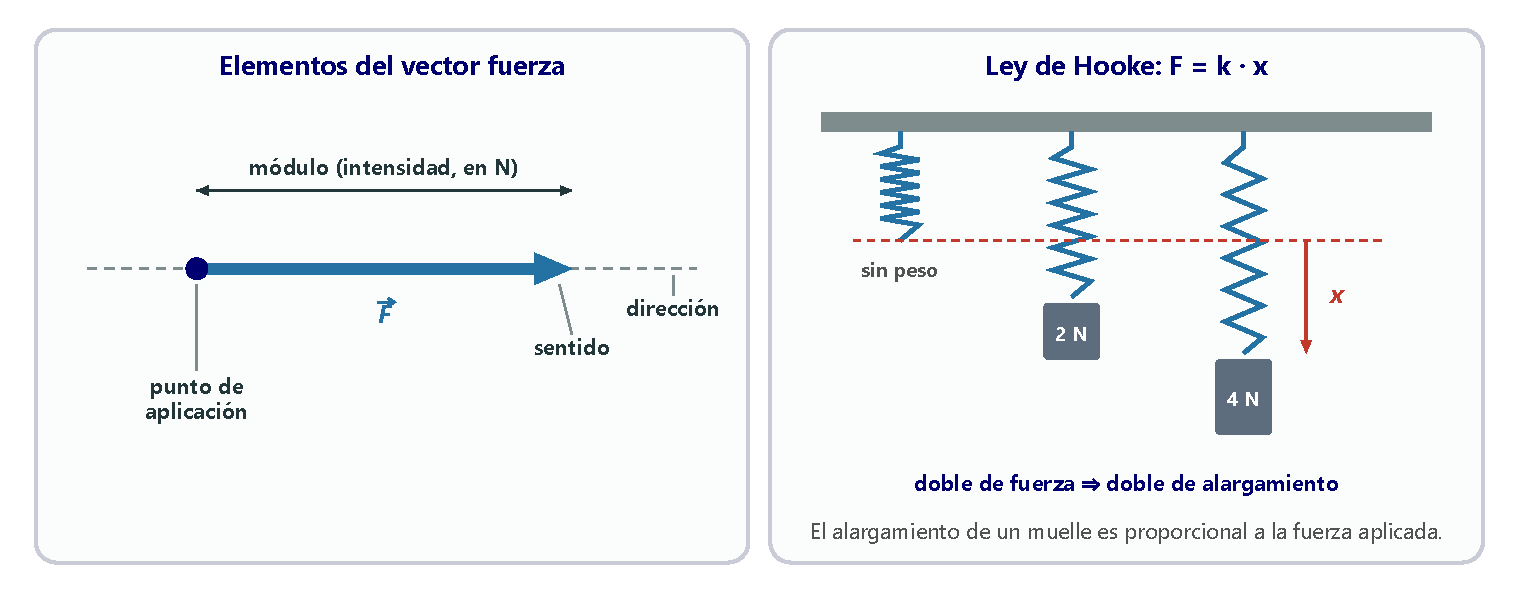
\includegraphics[width=0.85\textwidth]{images/UD10/vector_fuerza}
    \caption{Elementos de una fuerza y ley de Hooke: el alargamiento de un muelle es proporcional a la fuerza que lo estira.}
    \label{fig:ud10-vector}
\end{figure}

\subsection{Medida de las fuerzas}

Algunos materiales se deforman de manera proporcional a la fuerza que se les aplica, y esto permite medir fuerzas.

\begin{definition}[Dinamómetro]
    Es el instrumento que mide fuerzas. Consta de un muelle y una escala graduada, y se basa en la \textbf{ley de Hooke}:
    \[ F = k\,(L - L_0) = k\,\Delta L \]
    donde \(L_0\) es la longitud natural del muelle y \(L\) su longitud cuando actúa la fuerza.
\end{definition}

\begin{example}
    \textbf{Calibrar un muelle.} Un muelle mide \qty{15}{\cm} sin carga y \qty{18}{\cm} cuando se cuelga de él una pesa de
    \qty{6}{\newton}. a) ¿Cuál es su constante elástica? b) ¿Qué fuerza lo estira hasta \qty{22}{\cm}?

    \textbf{Solución.} a) \(k = \dfrac{F}{\Delta L} = \dfrac{6}{\num{0.03}} = \qty{200}{\newton\per\m}\).
    b) \(F = 200 \cdot \num{0.07} = \qty{14}{\newton}\).
\end{example}

\subsection{Clasificación de las fuerzas}

Las fuerzas nunca actúan aisladas: siempre son el resultado de una \textbf{interacción} entre, al menos, dos cuerpos. Podemos
clasificarlas de dos maneras.

\paragraph{Según la distancia entre los cuerpos.}
\begin{itemize}
    \item \textbf{Fuerzas de contacto}: necesitan que los cuerpos se toquen, como el empuje de una mano, la tensión de una cuerda o el
    rozamiento.
    \item \textbf{Fuerzas a distancia}: actúan sin contacto, como el peso o la atracción de un imán.
\end{itemize}

\paragraph{Interacciones fundamentales.} Todas las fuerzas de la naturaleza se deben, en último término, a cuatro tipos de
interacción entre partículas (tabla~\ref{tab:ud10-interacciones}). Las fuerzas de contacto, por ejemplo, son de origen
electromagnético: se deben a la repulsión entre los electrones de las superficies que se tocan.

\begin{table}[H]
    \centering
    \caption{Las cuatro interacciones fundamentales}
    \vspace{-5pt}
    \begin{tabular}{@{}lL{3.2cm}L{6.4cm}@{}}
        \toprule
        \textbf{Interacción} & \textbf{Alcance y carácter} & \textbf{Qué explica} \\
        \midrule
        Nuclear fuerte & Muy corto; atractiva; la más intensa & Mantiene unidos los quarks de protones y neutrones y estas
        partículas en el núcleo \\[3pt]
        Nuclear débil & Muy corto & Algunas desintegraciones radiactivas (como la desintegración beta) \\[3pt]
        Electromagnética & Largo; atractiva o repulsiva & Las propiedades de átomos y moléculas, la electricidad, el magnetismo, la
        luz y las fuerzas de contacto \\[3pt]
        Gravitatoria & Largo; siempre atractiva; la más débil & El peso, las mareas, el movimiento de los astros y la estructura del
        universo \\
        \bottomrule
    \end{tabular}
    \label{tab:ud10-interacciones}
\end{table}

\begin{remark}
    La física actual describe las interacciones mediante \textbf{campos}. Por ejemplo, en la teoría de la relatividad general de
    Einstein la gravedad no es una fuerza, sino una deformación del espacio-tiempo causada por la masa.
\end{remark}

\begin{exercise}
    Indica qué interacción fundamental actúa en cada caso: a) en una central nuclear se rompen núcleos de uranio; b) un imán atrae
    un clip; c) en un reactor experimental de fusión se unen núcleos de hidrógeno para formar helio; d) la Luna gira alrededor de la
    Tierra; e) un carbono-14 se transforma en nitrógeno-14 emitiendo un electrón.
    \begin{solu}
        a) \textcolor{red}{Nuclear fuerte} (y electromagnética, que separa los fragmentos). b) \textcolor{red}{Electromagnética}.
        c) \textcolor{red}{Nuclear fuerte} (y débil en algunas etapas). d) \textcolor{red}{Gravitatoria}. e) \textcolor{red}{Nuclear
        débil} (desintegración beta).
    \end{solu}
\end{exercise}

\begin{exercise}
    Clasifica estas fuerzas en fuerzas de contacto o a distancia: a) una grúa levanta un palé con un cable; b) un imán sujeta una
    nota en la nevera; c) un portero despeja el balón con los puños; d) el Sol atrae a Marte.
    \begin{solu}
        \textcolor{red}{De contacto: a y c. A distancia: b y d} (en b, también hay fuerzas de contacto entre la nota y la nevera).
    \end{solu}
\end{exercise}

%========================================================================================
\section{Componer y descomponer fuerzas}\label{sec:ud10-componer}
%========================================================================================

\textbf{Componer} fuerzas es sustituirlas por una sola que produzca el mismo efecto; \textbf{descomponer} una fuerza es sustituirla
por otras (sus componentes) cuya acción conjunta equivalga a ella. Ambos procedimientos son imprescindibles para resolver problemas
de equilibrio y de dinámica.

\subsection{Descomposición de una fuerza: componentes}

En el plano, cualquier fuerza \(\vec{F}\) que forme un ángulo \(\varphi\) con la parte positiva del eje \(X\) se puede escribir como la
suma de una fuerza paralela al eje \(X\) y otra paralela al eje \(Y\) (figura~\ref{fig:ud10-componentes}):
\[ \vec{F} = F_x\,\ivec + F_y\,\jvec = F\cos\varphi\;\ivec + F\sen\varphi\;\jvec \]

\begin{figure}[H]
    \centering
    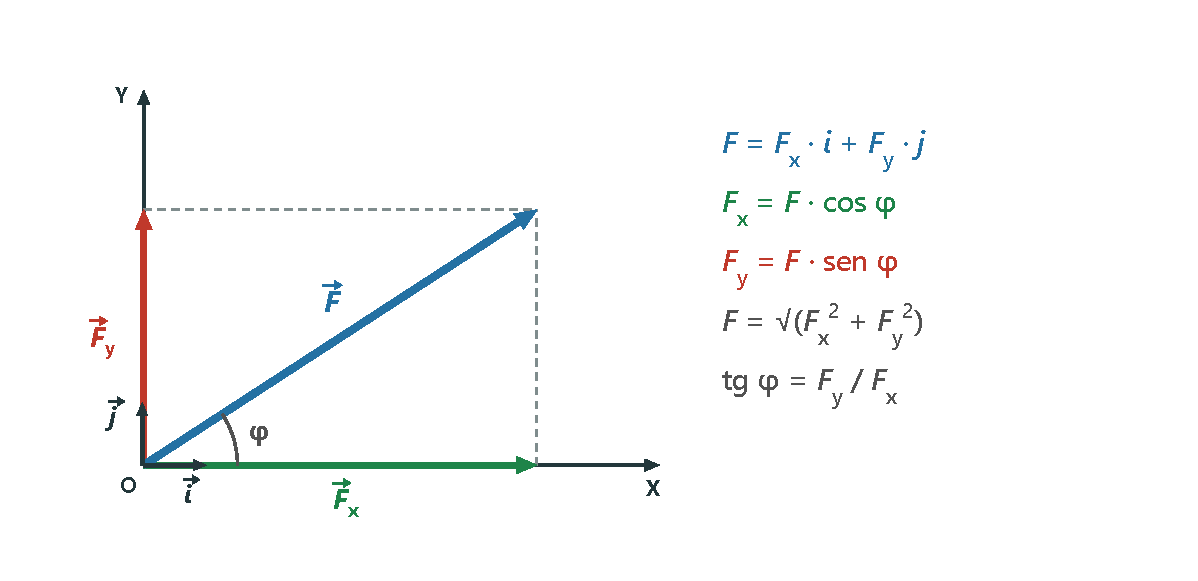
\includegraphics[width=0.75\textwidth]{images/UD10/descomposicion_fuerza}
    \caption{Componentes cartesianas de una fuerza. Conocidas las componentes, el módulo se obtiene con el teorema de Pitágoras y
    la dirección con la tangente.}
    \label{fig:ud10-componentes}
\end{figure}

\begin{example}
    \textbf{Tirar de un trineo.} Una persona tira de un trineo con una cuerda que forma \(30^\circ\) con el suelo, con una fuerza de
    \qty{500}{\newton}. Calcula las componentes horizontal y vertical de la fuerza y escríbela en forma vectorial.

    \textbf{Solución.} \(F_x = 500\cos 30^\circ = \qty{433}{\newton}\) (la que hace avanzar el trineo);
    \(F_y = 500\sen 30^\circ = \qty{250}{\newton}\) (tiende a levantarlo). En forma vectorial: \(\vec{F} = (433\,\ivec + 250\,\jvec)\)~N.
\end{example}

\subsection{Composición de fuerzas: fuerza resultante}

\begin{definition}[Fuerza resultante o neta]
    Es la suma vectorial de todas las fuerzas que actúan sobre un cuerpo, y produce por sí sola el mismo efecto que todas ellas:
    \[ \vec{F}_{\text{neta}} = \sum_{i=1}^{n} \vec{F}_i = \vec{F}_1 + \vec{F}_2 + \dots + \vec{F}_n
    = \Bigl(\sum F_{ix}\Bigr)\,\ivec + \Bigl(\sum F_{iy}\Bigr)\,\jvec \]
\end{definition}

Para fuerzas concurrentes, la resultante se calcula con la fórmula anterior (sumando componentes) o gráficamente. Hay casos
sencillos que conviene recordar (figura~\ref{fig:ud10-composicion}):

\begin{itemize}
    \item \textbf{Misma dirección y sentido}: los módulos se suman, \(F_{\text{neta}} = F_1 + F_2\).
    \item \textbf{Misma dirección y sentidos opuestos}: los módulos se restan, \(F_{\text{neta}} = |F_1 - F_2|\), y la resultante
    tiene el sentido de la mayor.
    \item \textbf{Fuerzas perpendiculares}: por el teorema de Pitágoras, \(F_{\text{neta}} = \sqrt{F_1^2 + F_2^2}\).
    \item \textbf{Cualquier ángulo \(\alpha\) entre ellas} (regla del paralelogramo):
    \(F_{\text{neta}} = \sqrt{F_1^2 + F_2^2 + 2F_1F_2\cos\alpha}\).
\end{itemize}

\begin{figure}[H]
    \centering
    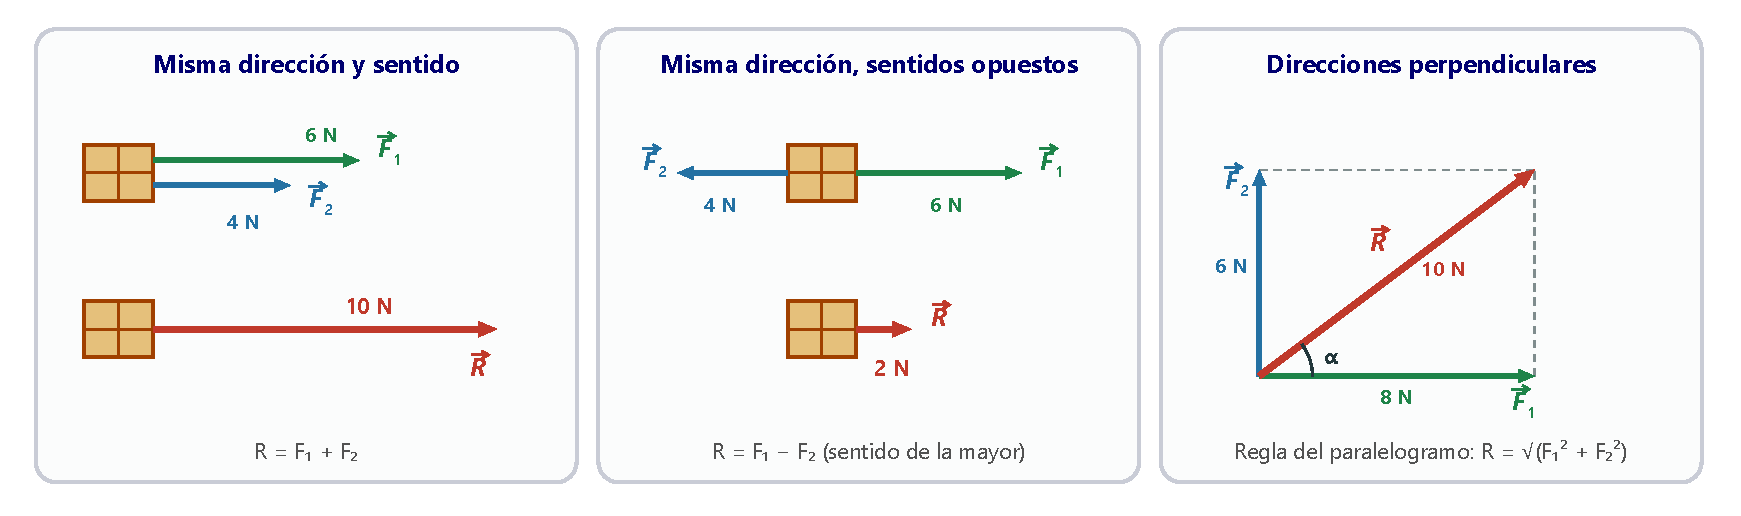
\includegraphics[width=\textwidth]{images/UD10/composicion_fuerzas}
    \caption{Resultante de dos fuerzas concurrentes en los tres casos más sencillos.}
    \label{fig:ud10-composicion}
\end{figure}

\begin{example}
    \textbf{Dos remolcadores.} Un buque mercante es arrastrado en el puerto por dos remolcadores que tiran en la misma dirección y
    sentido con fuerzas de \qty{2.6e5}{\newton} y \qty{3.4e5}{\newton}. a) ¿Qué fuerza total actúa sobre el buque? b) Si el buque
    pone en marcha sus motores en sentido contrario, con una fuerza de \qty{4.5e5}{\newton}, ¿cuál es la resultante?

    \textbf{Solución.} a) Misma dirección y sentido: \(F = \num{2.6e5} + \num{3.4e5} = \qty{6.0e5}{\newton}\).
    b) Sentidos opuestos: \(F' = \num{6.0e5} - \num{4.5e5} = \qty{1.5e5}{\newton}\), en el sentido de los remolcadores.
\end{example}

\begin{example}
    \textbf{Dos fuerzas que forman 60°.} Sobre un cuerpo actúan dos fuerzas de \qty{40}{\newton} y \qty{30}{\newton} que forman
    \(60^\circ\). Calcula el módulo de la resultante y el ángulo que forma con la fuerza mayor.

    \textbf{Solución.} Tomamos el eje \(X\) en la dirección de la fuerza de \qty{40}{\newton}:
    \(\vec{F}_1 = 40\,\ivec\) y \(\vec{F}_2 = 30\cos 60^\circ\,\ivec + 30\sen 60^\circ\,\jvec = 15\,\ivec + \num{25.98}\,\jvec\). Sumando:
    \(\vec{F} = 55\,\ivec + \num{25.98}\,\jvec\)~N.
    \[ F = \sqrt{55^2 + \num{25.98}^2} = \qty{60.8}{\newton} \qquad \tg\varphi = \frac{\num{25.98}}{55} \Rightarrow \varphi = \num{25.3}^\circ \]
    Con la regla del paralelogramo: \(F = \sqrt{1600 + 900 + 2 \cdot 40 \cdot 30 \cdot \cos 60^\circ} = \sqrt{3700} = \qty{60.8}{\newton}\).
\end{example}

\begin{exercise}
    Dibuja y calcula la resultante de tres fuerzas concurrentes de 16, 9 y \qty{25}{\newton}. Las fuerzas de 9 y \qty{25}{\newton}
    tienen la misma dirección y sentidos opuestos, y la de \qty{16}{\newton} es perpendicular a ellas.
    \begin{solu}
        \textcolor{blue}{En la dirección de las dos primeras: \(25 - 9 = \qty{16}{\newton}\); perpendicular: \qty{16}{\newton}.}
        \(F = \sqrt{16^2 + 16^2} = \textcolor{red}{\qty{22.6}{\newton}}\), formando \(45^\circ\) con cada dirección.
    \end{solu}
\end{exercise}

\begin{exercise}
    Calcula la resultante de \(\vec{F}_1 = (3\,\ivec + 5\,\jvec)\)~N, \(\vec{F}_2 = (-7\,\ivec + 2\,\jvec)\)~N y
    \(\vec{F}_3 = (6\,\ivec - 4\,\jvec)\)~N, su módulo y el ángulo que forma con el eje \(X\).
    \begin{solu}
        \(\vec{F} = (3 - 7 + 6)\,\ivec + (5 + 2 - 4)\,\jvec = \textcolor{red}{(2\,\ivec + 3\,\jvec)~\text{N}}\);
        \(F = \sqrt{13} = \textcolor{red}{\qty{3.61}{\newton}}\); \(\tg\varphi = \num{1.5} \Rightarrow \textcolor{red}{\varphi = \num{56.3}^\circ}\).
    \end{solu}
\end{exercise}

%========================================================================================
\section{El equilibrio}\label{sec:ud10-equilibrio}
%========================================================================================

En la vida diaria encontramos muchas situaciones de equilibrio: una persona haciendo una postura de yoga, un puente, un tren que
avanza por una vía recta a velocidad constante o una noria que gira siempre al mismo ritmo.

\subsection{Equilibrio de un cuerpo puntual}

\begin{definition}[Equilibrio de un cuerpo puntual]
    Un cuerpo puntual está en \textbf{equilibrio} si la resultante de todas las fuerzas que actúan sobre él es nula:
    \[ \sum \vec{F}_i = \vec{0} \quad\Longleftrightarrow\quad \sum F_{ix} = 0 \quad \text{y} \quad \sum F_{iy} = 0 \]
\end{definition}

\paragraph{Reposo y equilibrio.} Son conceptos distintos que a menudo se confunden:
\begin{itemize}
    \item Un cuerpo está en \textbf{reposo} si su velocidad es nula.
    \item Un cuerpo está en \textbf{equilibrio} si la fuerza neta sobre él es nula, es decir, si no tiene aceleración.
\end{itemize}
En un MRU hay \textbf{equilibrio sin reposo}: el cuerpo se mueve, pero sin aceleración. Y un objeto lanzado verticalmente hacia arriba
está en \textbf{reposo} instantáneo en el punto más alto, pero \textbf{no en equilibrio}, porque sobre él sigue actuando su peso.

\begin{figure}[H]
    \centering
    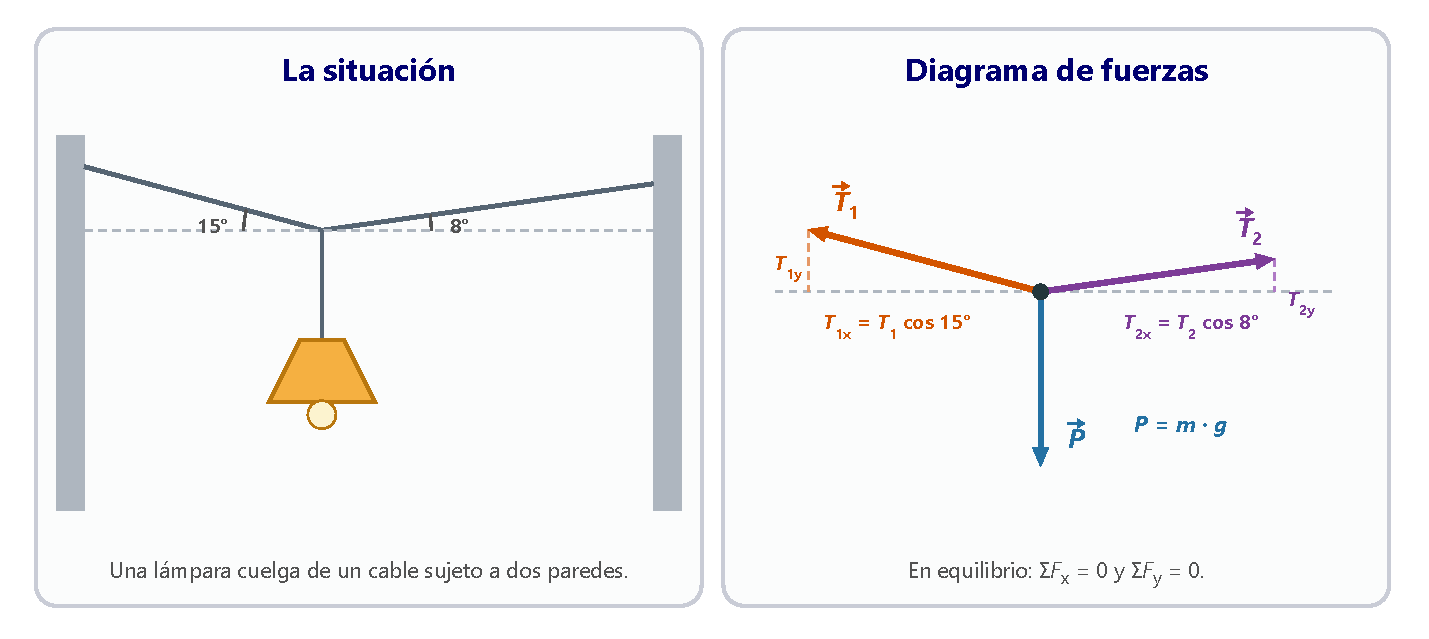
\includegraphics[width=0.95\textwidth]{images/UD10/equilibrio_cuerda}
    \caption{Un cuerpo colgado de un cable: el punto de unión está en equilibrio bajo la acción de las dos tensiones y el peso.}
    \label{fig:ud10-cuerda}
\end{figure}

\begin{example}
    \textbf{Una lámpara colgada de un cable.} Una lámpara de \qty{2.5}{\kg} cuelga del punto de un cable en el que este forma
    ángulos de \(15^\circ\) y \(8^\circ\) con la horizontal (figura~\ref{fig:ud10-cuerda}). Calcula la tensión de cada tramo del cable.

    \textbf{Solución.} Sobre el punto de unión actúan el peso, \(P = \num{2.5} \cdot \num{9.8} = \qty{24.5}{\newton}\), y las tensiones
    \(T_1\) (a la izquierda) y \(T_2\) (a la derecha). Aplicamos las condiciones de equilibrio:

    Eje \(X\): \(T_2\cos 8^\circ = T_1\cos 15^\circ \Rightarrow T_2 = \dfrac{\cos 15^\circ}{\cos 8^\circ}\,T_1 = \num{0.9754}\,T_1\)

    Eje \(Y\): \(T_1\sen 15^\circ + T_2\sen 8^\circ = P \Rightarrow T_1\,(\num{0.2588} + \num{0.9754} \cdot \num{0.1392}) = \num{24.5}\)
    \[ T_1 = \frac{\num{24.5}}{\num{0.3946}} = \qty{62.1}{\newton} \qquad T_2 = \num{0.9754} \cdot \num{62.1} = \qty{60.6}{\newton} \]
    Las tensiones son mucho mayores que el peso: cuanto más horizontal está un cable, más tenso tiene que estar para sujetar la carga.
\end{example}

\begin{exercise}
    Un contenedor de \qty{600}{\kg} cuelga de dos cables iguales que forman \(20^\circ\) con la horizontal. Calcula la tensión de
    cada cable.
    \begin{solu}
        \textcolor{blue}{Por simetría, las dos tensiones son iguales: \(2T\sen 20^\circ = m\,g\).}
        \(T = \dfrac{600 \cdot \num{9.8}}{2\sen 20^\circ} = \textcolor{red}{\qty{8.60e3}{\newton}}\).
    \end{solu}
\end{exercise}

\subsection{Momento de una fuerza}

Hasta ahora hemos supuesto que las fuerzas desplazan los cuerpos (traslación), pero también pueden hacerlos \textbf{girar}. Si la
línea de acción de una fuerza no pasa por el centro de masas de un cuerpo o por su eje de giro, la fuerza produce una
\textbf{rotación}. La magnitud que mide esta capacidad es el \textbf{momento de la fuerza}.

\begin{definition}[Momento de una fuerza]
    El momento de una fuerza \(\vec{F}\) respecto a un punto O es el vector
    \[ \vec{M} = \vec{r} \times \vec{F} \]
    donde \(\vec{r}\) es el vector de posición del punto de aplicación de la fuerza respecto a O. Mide la capacidad de la fuerza para
    cambiar la velocidad de giro del cuerpo.
\end{definition}

Sus características son (figura~\ref{fig:ud10-momento}):
\begin{itemize}
    \item \textbf{Módulo}: \(M = r\,F\sen\varphi\), donde \(\varphi\) es el ángulo entre \(\vec{r}\) y \(\vec{F}\). Se mide en
    \unit{\newton\metre}.
    \item \textbf{Dirección}: perpendicular al plano formado por \(\vec{r}\) y \(\vec{F}\) (la del eje de giro).
    \item \textbf{Sentido}: por convenio, positivo si el giro es antihorario y negativo si es horario.
\end{itemize}
Si la línea de acción de la fuerza pasa por O (\(\varphi = 0^\circ\) o \(180^\circ\)), el momento es nulo: empujar una puerta hacia
las bisagras no la hace girar.

\begin{figure}[H]
    \centering
    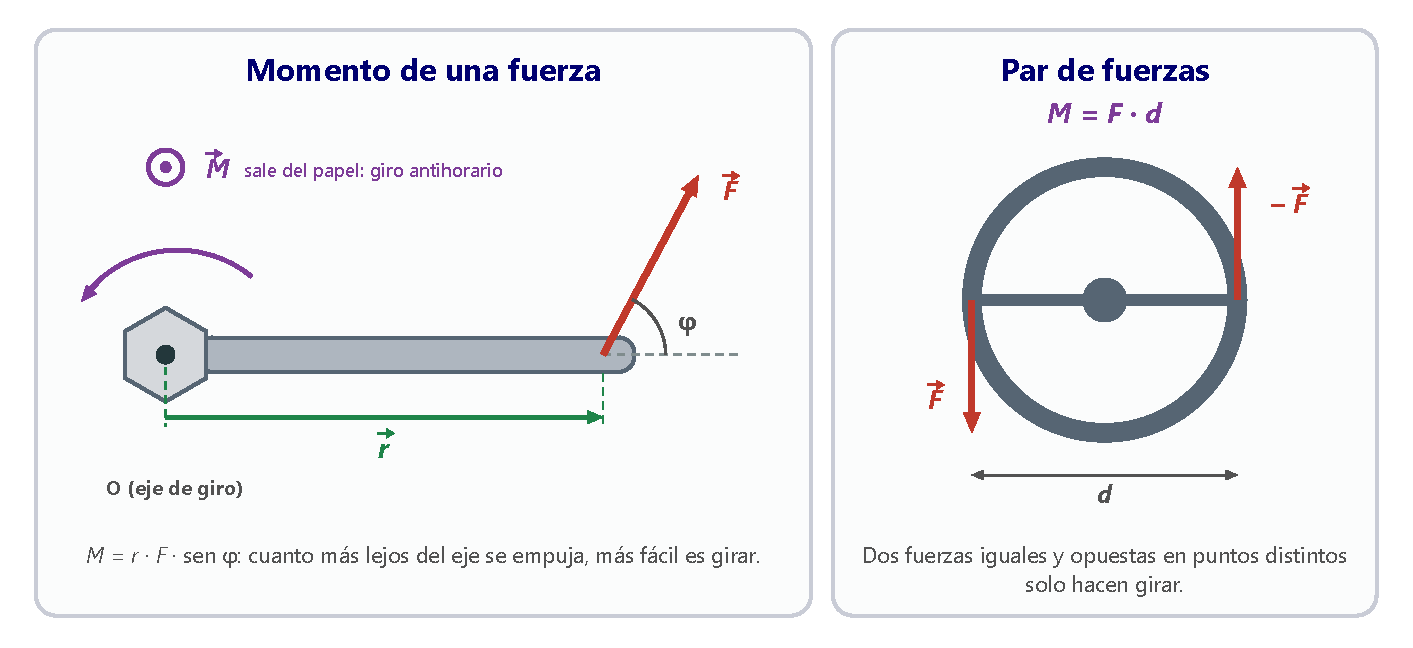
\includegraphics[width=0.95\textwidth]{images/UD10/momento_fuerza}
    \caption{Momento de una fuerza aplicada a una llave inglesa y par de fuerzas sobre un volante.}
    \label{fig:ud10-momento}
\end{figure}

\begin{definition}[Par de fuerzas]
    Un \textbf{par de fuerzas} son dos fuerzas paralelas, de igual módulo y sentidos contrarios, aplicadas en puntos distintos. Su
    resultante es nula, así que no trasladan el cuerpo, pero lo hacen girar con un momento \(M = F\,d\), donde \(d\) es la distancia
    entre sus líneas de acción. Es lo que hacemos al girar un volante o un grifo.
\end{definition}

\begin{example}
    \textbf{Cambiar una rueda.} Para aflojar una tuerca se usa una llave de \qty{30}{\cm} y se aplica en su extremo una fuerza de
    \qty{80}{\newton}. a) Calcula el momento si la fuerza es perpendicular a la llave. b) ¿Y si forma \(60^\circ\) con ella?

    \textbf{Solución.} a) \(M = r\,F\sen 90^\circ = \num{0.30} \cdot 80 \cdot 1 = \qty{24}{\newton\metre}\).
    b) \(M = \num{0.30} \cdot 80 \cdot \sen 60^\circ = \qty{20.8}{\newton\metre}\). El momento es máximo cuando la fuerza es
    perpendicular a la llave.
\end{example}

\subsection{Equilibrio de un cuerpo extenso}

Una fuerza neta hace que un cuerpo empiece a trasladarse o cambie su movimiento de traslación; un momento neto hace que empiece a
girar o cambie su rotación.

\begin{definition}[Condiciones de equilibrio de un sólido]
    Un cuerpo extenso está en equilibrio si son nulas la resultante de las fuerzas y la resultante de los momentos respecto a
    cualquier punto:
    \[ \sum \vec{F}_i = \vec{0} \qquad \sum \vec{M}_i = \vec{0} \]
\end{definition}

\begin{remark}
    Hay tres tipos de equilibrio: \textbf{estático} (el cuerpo está en reposo, como una persona en una postura de yoga),
    \textbf{dinámico} (se traslada con velocidad constante, como un tren en una recta) y \textbf{rotacional} (gira con velocidad angular
    constante, como una rueda de molino).
\end{remark}

\begin{example}
    \textbf{Transportar un saco.} Dos personas llevan un saco de \qty{60}{\kg} colgado de una barra de peso despreciable. Una está a
    \qty{0.9}{\m} del saco y la otra a \qty{1.5}{\m}. ¿Qué fuerza hace cada una?

    \textbf{Solución.} El peso del saco es \(P = 60 \cdot \num{9.8} = \qty{588}{\newton}\). Condiciones de equilibrio:
    \[ \sum F = 0:\; F_1 + F_2 = P \qquad \sum M_{\text{saco}} = 0:\; F_1 \cdot \num{0.9} = F_2 \cdot \num{1.5} \]
    Tomando momentos respecto al punto del que cuelga el saco (así el peso no da momento):
    \(F_1 = \dfrac{\num{1.5}}{\num{0.9}}\,F_2\). Sustituyendo: \(F_2\left(1 + \dfrac{\num{1.5}}{\num{0.9}}\right) = 588 \Rightarrow
    F_2 = \qty{220.5}{\newton}\) y \(F_1 = \qty{367.5}{\newton}\). Hace más fuerza la persona que está \textbf{más cerca} del saco.
\end{example}

\begin{exercise}
    Dos fuerzas paralelas de \qty{10}{\newton} y \qty{40}{\newton}, ambas hacia abajo, actúan en los extremos de una barra de
    \qty{2.5}{\m} de peso despreciable. ¿Dónde hay que colocar el punto de apoyo para que la barra esté en equilibrio? ¿Qué fuerza
    hace el apoyo?
    \begin{solu}
        \textcolor{blue}{Momentos respecto al apoyo, a una distancia \(x\) de la fuerza de \qty{10}{\newton}: \(10\,x = 40\,(\num{2.5} - x)\).}
        \(x = \textcolor{red}{\qty{2}{\m}}\) de la fuerza de \qty{10}{\newton} (a \qty{0.5}{\m} de la de \qty{40}{\newton}). El
        apoyo hace \(\textcolor{red}{\qty{50}{\newton}}\) hacia arriba.
    \end{solu}
\end{exercise}

\begin{exercise}
    El tablero de una mesa mide \qty{2.4}{\m} y pesa \qty{60}{\newton}. Se apoya en dos caballetes: uno en un extremo y otro a
    \qty{0.6}{\m} del otro extremo. Calcula la fuerza que hace cada caballete.
    \begin{solu}
        \textcolor{blue}{El peso actúa en el centro del tablero, a \qty{1.2}{\m} del extremo apoyado.}
        \textcolor{blue}{Los caballetes distan \qty{1.8}{\m}.} Tomamos momentos respecto al caballete del extremo:
        \[ F_B \cdot \num{1.8} = 60 \cdot \num{1.2} \]
        \(\textcolor{red}{F_B = \qty{40}{\newton}}\) y \(\textcolor{red}{F_A = 60 - 40 = \qty{20}{\newton}}\).
    \end{solu}
\end{exercise}

\begin{exercise}
    Para abrir una puerta de \qty{85}{\cm} de anchura hace falta un momento de \qty{1.5}{\newton\metre}. Si empujamos
    perpendicularmente junto al pomo con una fuerza de \qty{2}{\newton}, ¿se abrirá? ¿Y si empujamos con la misma fuerza a
    \qty{40}{\cm} de las bisagras?
    \begin{solu}
        Junto al pomo: \(M = \num{0.85} \cdot 2 = \qty{1.7}{\newton\metre}\), \textcolor{red}{sí se abre}. A \qty{40}{\cm}:
        \(M = \num{0.40} \cdot 2 = \qty{0.8}{\newton\metre}\), \textcolor{red}{no se abre}.
    \end{solu}
\end{exercise}

%========================================================================================
\section{Las leyes de Newton}\label{sec:ud10-newton}
%========================================================================================

La \textbf{dinámica} es la parte de la física que estudia el movimiento de los cuerpos atendiendo a sus causas, las fuerzas. Toda la
dinámica clásica se basa en las tres \textbf{leyes de Newton}, que relacionan las fuerzas que actúan sobre un cuerpo con su movimiento.
Newton las publicó en 1687 en su obra \textit{Philosophiae Naturalis Principia Mathematica}.

\subsection{Primera ley de Newton: principio de inercia}

Cuando vamos en moto y arrancamos, notamos que nos vamos hacia atrás; si frenamos de golpe, nos vamos hacia delante. En ambos casos
el cuerpo tiende a \textbf{mantener su estado}: en reposo o moviéndose en línea recta a velocidad constante. Solo cuando el asiento
o el manillar nos empujan pasamos a movernos con la moto.

\begin{definition}[Inercia]
    Es la tendencia de un cuerpo a mantener su estado de reposo o de movimiento rectilíneo uniforme. Es una propiedad de toda la
    materia y está ligada a la masa: cuanto mayor es la masa, mayor es la inercia.
\end{definition}

\begin{definition}[Primera ley de Newton o principio de inercia]
    Si sobre un cuerpo no actúa ninguna fuerza, o la resultante de las que actúan es nula, el cuerpo permanece en reposo o se mueve
    con movimiento rectilíneo uniforme:
    \[ \sum \vec{F}_i = \vec{0} \quad\Longrightarrow\quad \vec{v} = \text{constante} \]
\end{definition}

Si la velocidad constante es \(\vec{0}\), el cuerpo está en reposo; si es distinta de cero, el cuerpo describe un MRU.

\paragraph{Sistemas de referencia inerciales.} Un \textbf{sistema de referencia inercial} es aquel en el que se cumple el principio
de inercia. Todos los sistemas que se mueven con MRU respecto a uno inercial son también inerciales.

\begin{definition}[Principio de relatividad de Galileo]
    Las leyes de la mecánica son las mismas en todos los sistemas de referencia inerciales.
\end{definition}

Por eso, con experimentos mecánicos es imposible distinguir si un sistema inercial está en reposo o se mueve con MRU: \textbf{no se
puede medir el movimiento absoluto}. El tiempo, la masa y las fuerzas tienen el mismo valor en todos los sistemas inerciales: son
\textbf{invariantes de Galileo}. Einstein amplió este principio a todas las leyes de la física en su teoría de la relatividad
(1905), en la que longitudes y tiempos sí dependen del sistema de referencia cuando las velocidades se acercan a la de la luz.

\begin{remark}
    En rigor, la Tierra \textbf{no} es un sistema inercial, porque gira sobre sí misma y alrededor del Sol. Pero sus aceleraciones
    son tan pequeñas que, para la mayoría de los movimientos cotidianos, podemos tratarla como si lo fuera.
\end{remark}

\begin{example}
    \textbf{En un avión.} Explica qué le ocurre a una persona sentada en un avión cuando: a) el avión gira hacia la izquierda;
    b) despega; c) aterriza y frena; d) desciende bruscamente.

    \textbf{Solución.} Por el principio de inercia, la persona tiende a seguir moviéndose como lo hacía: a) sigue en línea recta,
    así que respecto al avión se desplaza hacia la \textbf{derecha}; b) tiende a quedarse atrás y se siente \textbf{empujada contra el
    respaldo}; c) sigue moviéndose y se va \textbf{hacia delante}; d) tiende a seguir a la misma altura, así que se siente
    \textbf{levantada del asiento}.
\end{example}

\begin{exercise}
    Cuando viajamos con una mascota en el coche, la ley obliga a llevarla sujeta y separada del conductor. Explica por qué con la
    primera ley de Newton. ¿Qué ocurriría con la mascota y con los pasajeros sin cinturón en un frenazo brusco?
    \begin{solu}
        \textcolor{red}{En un frenazo, por inercia, todo lo que no está sujeto sigue moviéndose hacia delante a la velocidad que
        llevaba el coche} y choca contra los asientos, el parabrisas o los pasajeros. Los cinturones y los arneses ejercen la fuerza
        necesaria para frenarlos junto con el coche.
    \end{solu}
\end{exercise}

\begin{exercise}
    En un truco de magia se tira bruscamente de un mantel y los platos y vasos que hay encima apenas se mueven. Explica el fenómeno
    y propón otros ejemplos basados en el mismo principio.
    \begin{solu}
        Es el \textcolor{red}{principio de inercia}: si el tirón es muy rápido, la fuerza de rozamiento actúa durante muy poco tiempo
        y apenas cambia el estado de reposo de los platos. Otros ejemplos: la moneda sobre una cartulina que se retira de un golpe
        (práctica~\ref{sec:ud10-practicas}), quitar una pieza de la base de una torre de bloques de un golpe seco, sacudir una
        alfombra para quitarle el polvo.
    \end{solu}
\end{exercise}

\subsection{Segunda ley de Newton: principio fundamental de la dinámica}

La primera ley describe qué ocurre cuando la fuerza neta es nula. La segunda explica qué ocurre cuando no lo es: la fuerza neta es
la responsable de los \textbf{cambios} de velocidad.

\begin{definition}[Segunda ley de Newton o principio fundamental de la dinámica]
    La fuerza neta que actúa sobre un cuerpo le produce una aceleración de la misma dirección y sentido, directamente proporcional a
    la fuerza e inversamente proporcional a la masa del cuerpo:
    \[ \sum \vec{F}_i = \vec{F}_{\text{neta}} = m\,\vec{a} \]
\end{definition}

Si se aplican a un mismo cuerpo distintas fuerzas, el cociente entre cada fuerza y la aceleración que produce es siempre el mismo, la
masa inercial: \(\dfrac{F_1}{a_1} = \dfrac{F_2}{a_2} = \dots = m\). Cuanto mayor es la masa de un cuerpo, mayor es su inercia y más
fuerza hace falta para cambiar su movimiento. De esta ley sale la definición del newton: \textbf{\qty{1}{\newton} es la fuerza que
comunica a una masa de \qty{1}{\kg} una aceleración de \qty{1}{\m\per\s\squared}}.

\begin{remark}
    La fuerza neta y la aceleración tienen siempre la misma dirección y sentido, pero no necesariamente la velocidad. Conocidas la
    velocidad inicial y la aceleración, las ecuaciones de la cinemática de la unidad anterior nos dicen cómo evoluciona el movimiento.
\end{remark}

\paragraph{Cómo resolver un problema de dinámica.}
\begin{enumerate}[label=\numberballgreen]
    \item Dibuja \textbf{todas las fuerzas} que actúan sobre el cuerpo (y solo esas).
    \item Elige unos ejes: uno en la dirección del movimiento y otro perpendicular.
    \item Descompón las fuerzas que no estén sobre los ejes.
    \item Aplica \(\sum F_x = m\,a\) en la dirección del movimiento y \(\sum F_y = 0\) en la perpendicular.
\end{enumerate}

\begin{example}
    \textbf{Una grúa remolca un coche.} Una grúa arrastra un coche averiado de \qty{1100}{\kg} con un cable que forma \(20^\circ\)
    con la horizontal y ejerce una fuerza de \qty{12000}{\newton}. La fuerza de rozamiento es de \qty{3500}{\newton}. Calcula: a) la
    aceleración del coche; b) la distancia que recorre en \qty{5}{\s} si parte del reposo.

    \textbf{Solución.} a) En el eje del movimiento actúan la componente horizontal de la fuerza del cable y el rozamiento:
    \[ F_x = 12000\cos 20^\circ = \qty{11276}{\newton} \qquad F_x - F_r = m\,a \Rightarrow a = \frac{11276 - 3500}{1100} = \qty{7.07}{\m\per\s\squared} \]
    (En el eje vertical no hay aceleración: el peso queda compensado por la normal y la componente vertical de la fuerza del cable.)

    b) Con la ecuación del MRUA: \(x = \dfrac{1}{2}\,a\,t^2 = \dfrac{1}{2} \cdot \num{7.07} \cdot 5^2 = \qty{88.4}{\m}\).
\end{example}

\paragraph{El plano inclinado.} Sobre un cuerpo apoyado en un plano inclinado un ángulo \(\alpha\) actúan su peso, la normal y, si
lo hay, el rozamiento. Conviene tomar un eje paralelo al plano y otro perpendicular, y descomponer el peso
(figura~\ref{fig:ud10-plano}):
\[ P_x = m\,g\sen\alpha \qquad P_y = m\,g\cos\alpha \]
La componente paralela, \(P_x\), hace bajar el cuerpo; la perpendicular, \(P_y\), la equilibra la normal.

\begin{figure}[H]
    \centering
    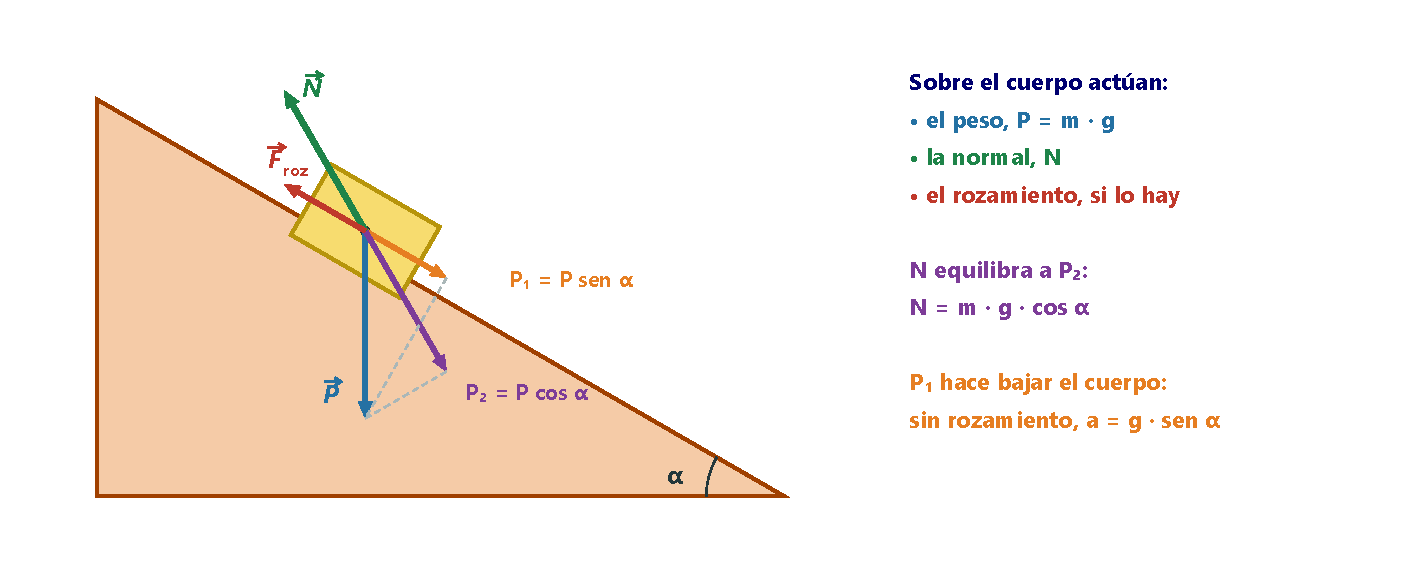
\includegraphics[width=0.85\textwidth]{images/UD10/plano_inclinado}
    \caption{Fuerzas sobre un cuerpo en un plano inclinado. Las componentes del peso se nombran aquí \(P_1\) (paralela) y \(P_2\)
    (perpendicular).}
    \label{fig:ud10-plano}
\end{figure}

\begin{example}
    \textbf{Una bola por una rampa.} Una bola de \qty{2}{\kg} baja por un plano inclinado \(25^\circ\) y sobre ella actúa una fuerza
    de rozamiento de \qty{2}{\newton}. Calcula: a) su aceleración; b) el tiempo que tarda en recorrer \qty{6}{\m} si parte del reposo.

    \textbf{Solución.} a) Peso: \(P = 2 \cdot \num{9.8} = \qty{19.6}{\newton}\); \(P_x = \num{19.6}\sen 25^\circ = \qty{8.28}{\newton}\);
    \(P_y = \num{19.6}\cos 25^\circ = \qty{17.8}{\newton} = N\).
    \[ P_x - F_r = m\,a \Rightarrow a = \frac{\num{8.28} - 2}{2} = \qty{3.14}{\m\per\s\squared} \]
    b) \(x = \dfrac{1}{2}\,a\,t^2 \Rightarrow t = \sqrt{\dfrac{2x}{a}} = \sqrt{\dfrac{2 \cdot 6}{\num{3.14}}} = \qty{1.95}{\s}\).
\end{example}

\begin{exercise}
    Una caja de \qty{90}{\kg}, en reposo sobre el suelo, es empujada horizontalmente con una fuerza de \qty{320}{\newton}. Si la
    fuerza de rozamiento es de \qty{230}{\newton}, ¿qué velocidad tendrá al cabo de \qty{4}{\s}?
    \begin{solu}
        \(a = \dfrac{320 - 230}{90} = \qty{1}{\m\per\s\squared}\); \(v = a\,t = \textcolor{red}{\qty{4}{\m\per\s}}\).
    \end{solu}
\end{exercise}

\begin{exercise}
    Sobre un sillón de \qty{70}{\kg} en reposo se aplica una fuerza horizontal de \qty{420}{\newton}. El rozamiento es de
    \qty{280}{\newton}. Calcula: a) la aceleración; b) la velocidad y la distancia recorrida en \qty{4}{\s}.
    \begin{solu}
        a) \(a = \dfrac{420 - 280}{70} = \textcolor{red}{\qty{2}{\m\per\s\squared}}\). b) \(v = 2 \cdot 4 = \textcolor{red}{\qty{8}{\m\per\s}}\);
        \(x = \frac{1}{2} \cdot 2 \cdot 4^2 = \textcolor{red}{\qty{16}{\m}}\).
    \end{solu}
\end{exercise}

\begin{exercise}
    Un técnico de sonido sube unos altavoces de \qty{70}{\kg} por una rampa inclinada \(15^\circ\). Si el rozamiento es de
    \qty{150}{\newton}, ¿qué fuerza mínima, paralela a la rampa, debe hacer?
    \begin{solu}
        \textcolor{blue}{La fuerza mínima es la que consigue que suban a velocidad constante (\(a = 0\)):}
        \(F = m\,g\sen 15^\circ + F_r = \num{177.5} + 150 = \textcolor{red}{\qty{328}{\newton}}\).
    \end{solu}
\end{exercise}

\begin{exercise}
    Sobre un cuerpo de \qty{8}{\kg} situado en un plano inclinado \(30^\circ\) se aplica una fuerza de \qty{12}{\newton} paralela
    al plano y hacia abajo. El rozamiento es de \qty{10}{\newton}. a) Calcula la aceleración. b) Si se retira la fuerza de
    \qty{12}{\newton}, ¿qué fuerza hay que aplicar hacia arriba para que el cuerpo baje con velocidad constante?
    \begin{solu}
        \(P_x = 8 \cdot \num{9.8} \cdot \sen 30^\circ = \qty{39.2}{\newton}\). a) \(a = \dfrac{12 + \num{39.2} - 10}{8} =
        \textcolor{red}{\qty{5.15}{\m\per\s\squared}}\). b) \(F + F_r = P_x \Rightarrow F = \num{39.2} - 10 =
        \textcolor{red}{\qty{29.2}{\newton}}\).
    \end{solu}
\end{exercise}

\subsection{Tercera ley de Newton: principio de acción y reacción}

Las dos primeras leyes se fijan en un solo cuerpo y en las fuerzas que actúan sobre él. La tercera nos recuerda que una fuerza es
siempre una \textbf{interacción} entre dos cuerpos: un cuerpo no puede, por sí solo, cambiar su estado de movimiento.

\begin{definition}[Tercera ley de Newton o principio de acción y reacción]
    Si un cuerpo A ejerce una fuerza sobre un cuerpo B, el cuerpo B ejerce sobre A una fuerza de igual módulo y dirección y de
    sentido contrario:
    \[ \vec{F}_{AB} = -\vec{F}_{BA} \]
    A estas dos fuerzas se las llama \textbf{acción} y \textbf{reacción}.
\end{definition}

Hay que tener en cuenta que:
\begin{itemize}
    \item Las fuerzas siempre aparecen \textbf{por pares}: a cada acción le corresponde una reacción.
    \item Acción y reacción son \textbf{simultáneas}: no hay una primera y otra después.
    \item Actúan sobre \textbf{cuerpos distintos}, por lo que \textbf{no se anulan} entre sí. Sus efectos pueden ser muy diferentes: el
    cuerpo de mayor masa adquiere menor aceleración.
\end{itemize}

\begin{figure}[H]
    \centering
    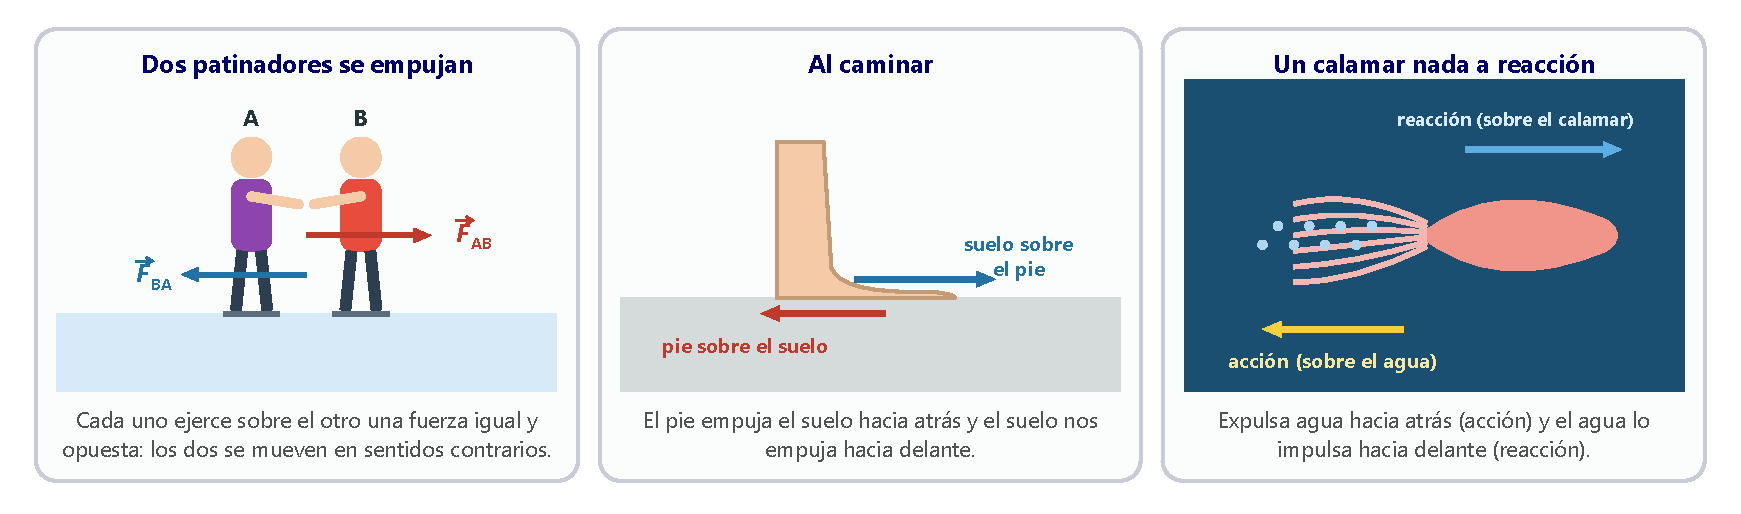
\includegraphics[width=\textwidth]{images/UD10/accion_reaccion}
    \caption{Ejemplos de pares de fuerzas de acción y reacción.}
    \label{fig:ud10-accion}
\end{figure}

\begin{example}
    \textbf{Acción y reacción en la vida diaria.} Explica con la tercera ley: a) el choque de dos coches; b) el despegue de un cohete;
    c) el golpe de una raqueta a una pelota.

    \textbf{Solución.} a) Cada coche ejerce sobre el otro una fuerza igual y opuesta; los dos se deforman y cambian su velocidad, más
    el de menor masa. b) El cohete expulsa los gases de la combustión hacia abajo y los gases empujan al cohete hacia arriba con una
    fuerza igual. c) La raqueta empuja la pelota y, a la vez, la pelota empuja la raqueta hacia atrás (lo nota la muñeca del jugador).
\end{example}

\begin{exercise}
    ¿Cuáles de los siguientes pares de fuerzas son de acción y reacción? a) Un boxeador golpea un saco y el saco empuja el puño.
    b) Un león arrastra una presa y el suelo frena la presa con el rozamiento. c) El peso de una persona sentada y la fuerza normal
    que le hace la silla. d) Dos patinadores sobre hielo se empujan.
    \begin{solu}
        \textcolor{red}{Son de acción y reacción a y d.} En b y c las dos fuerzas actúan sobre el \textbf{mismo} cuerpo (la presa; la
        persona), así que no pueden ser un par de acción y reacción. La reacción al peso de la persona es la fuerza con que ella atrae
        a la Tierra, y la reacción a la normal es la fuerza con que la persona empuja la silla.
    \end{solu}
\end{exercise}

\begin{table}[H]
    \centering
    \caption{Resumen de las tres leyes de la dinámica}
    \vspace{-5pt}
    \begin{tabular}{@{}lL{5.2cm}c@{}}
        \toprule
        \textbf{Ley} & \textbf{Qué dice} & \textbf{Expresión} \\
        \midrule
        Primera (inercia) & Sin fuerza neta, un cuerpo sigue en reposo o con MRU & \(\sum \vec{F} = \vec{0} \Rightarrow \vec{v} = \text{cte}\) \\[3pt]
        Segunda (fundamental) & La fuerza neta produce una aceleración proporcional & \(\sum \vec{F} = m\,\vec{a}\) \\[3pt]
        Tercera (acción y reacción) & Las fuerzas aparecen por pares iguales y opuestos, sobre cuerpos distintos & \(\vec{F}_{AB} = -\vec{F}_{BA}\) \\
        \bottomrule
    \end{tabular}
    \label{tab:ud10-leyes}
\end{table}

%========================================================================================
\section{Momento lineal o cantidad de movimiento}\label{sec:ud10-momento-lineal}
%========================================================================================

Piensa en estas dos situaciones: ¿cuesta lo mismo poner en movimiento a dos patinadores de distinta masa? ¿Hace falta la misma fuerza
para frenar dos coches iguales que van a distinta velocidad? La dificultad para cambiar el movimiento de un cuerpo depende a la vez
de su \textbf{masa} y de su \textbf{velocidad}. La magnitud que reúne ambas es el \textbf{momento lineal}.

\subsection{Concepto de momento lineal}

\begin{definition}[Momento lineal o cantidad de movimiento]
    Es el producto de la masa de un cuerpo por su velocidad:
    \[ \vec{p} = m\,\vec{v} \]
    Es un vector con la dirección y el sentido de la velocidad. Su unidad en el SI es el \unit{\kg\m\per\s}.
\end{definition}

El momento lineal mide la «cantidad de movimiento» de un cuerpo y su capacidad para transmitir movimiento a otros cuerpos. Cuando
hablamos de un \textbf{sistema} nos referimos a la parte del universo que estudiamos: puede ser un solo cuerpo o un conjunto de
partículas. El momento lineal de un sistema es la suma de los momentos lineales de sus partes.

\subsection{La formulación general de la segunda ley}

Newton enunció su segunda ley usando el momento lineal, y esa es su forma más general:

\begin{definition}[Ecuación fundamental de la dinámica]
    La fuerza neta exterior que actúa sobre un sistema es igual a la variación por unidad de tiempo de su momento lineal:
    \[ \vec{F}_{\text{neta}} = \lim_{\Delta t \to 0} \frac{\Delta\vec{p}}{\Delta t} = \frac{\dif\vec{p}}{\dif t} \]
\end{definition}

Derivando el producto \(m\,\vec{v}\):
\[ \vec{F}_{\text{neta}} = \frac{\dif(m\,\vec{v})}{\dif t} = \frac{\dif m}{\dif t}\,\vec{v} + m\,\frac{\dif\vec{v}}{\dif t} \]
Solo si la masa es constante, \(\dfrac{\dif m}{\dif t} = 0\), y recuperamos la expresión conocida: \(\vec{F}_{\text{neta}} = m\,\vec{a}\).
Hay cuerpos cuya masa cambia mientras se mueven, como un cohete que quema combustible o un globo que suelta lastre, y para ellos hay
que usar la forma general.

\begin{example}
    \textbf{Frenar con un patinete.} Una persona en patinete eléctrico circula a \qty{24}{\km\per\hour}. Ve un obstáculo y frena
    durante \qty{1.2}{\s}, hasta \qty{9}{\km\per\hour}. Si la masa de la persona y el patinete es de \qty{90}{\kg}, calcula: a) la
    variación del momento lineal; b) la fuerza media de frenado.

    \textbf{Solución.} Pasamos las velocidades al SI: \(v_1 = \qty{6.67}{\m\per\s}\) y \(v_2 = \qty{2.5}{\m\per\s}\).
    a) \(\Delta p = m\,(v_2 - v_1) = 90 \cdot (\num{2.5} - \num{6.67}) = \qty{-375}{\kg\m\per\s}\).
    b) \(F = \dfrac{\Delta p}{\Delta t} = \dfrac{-375}{\num{1.2}} = \qty{-312.5}{\newton}\); el signo indica que la fuerza se opone al
    movimiento. (Como todo ocurre en una dirección, trabajamos con las componentes sin escribir el vector unitario.)
\end{example}

\subsection{Impulso mecánico}

Cuando empujamos un carrito, la velocidad que alcanza es tanto mayor cuanto más fuerte empujamos y cuanto más tiempo lo hacemos. La
magnitud que combina ambas cosas es el \textbf{impulso}.

\begin{definition}[Impulso mecánico]
    Para una fuerza constante, el impulso es el producto de la fuerza neta por el tiempo durante el que actúa:
    \[ \vec{I} = \vec{F}_{\text{neta}}\,\Delta t \]
    Tiene la dirección y el sentido de la fuerza. Su unidad en el SI es el \unit{\newton\s}, que equivale a \unit{\kg\m\per\s}.
\end{definition}

En los golpes (un saque de tenis, una patada a un balón) la fuerza cambia mucho durante el contacto. Entonces se usa la \textbf{fuerza
media}, la fuerza constante que daría el mismo impulso: el área bajo la curva \(F\)-\(t\) es igual al área del rectángulo de altura
\(F_{\text{media}}\) (figura~\ref{fig:ud10-impulso}).

\begin{figure}[H]
    \centering
    \begin{tikzpicture}
        \begin{axis}[grafica, width=0.5\linewidth, height=5cm, xlabel={\(t\)}, ylabel={\(F\)}, xmin=0, xmax=10, ymin=0, ymax=11,
            xtick={2.6,7.4}, xticklabels={\(t_1\),\(t_2\)}, ytick={4.62}, yticklabels={\(F_{\text{media}}\)}]
            \addplot[fill=ocre!25, draw=none, domain=2.6:7.4] {10*exp(-((x-5)^2)/1.4)} \closedcycle;
            \addplot[very thick, red!70!black, domain=1:9] {10*exp(-((x-5)^2)/1.4)};
            \addplot[thick, blue!70!black, dashed, domain=2.6:7.4] {4.62};
            \draw[dashed, gray] (axis cs:2.6,0) -- (axis cs:2.6,4.62);
            \draw[dashed, gray] (axis cs:7.4,0) -- (axis cs:7.4,4.62);
            \node[font=\scriptsize] at (axis cs:5,2) {\(I\) = área};
        \end{axis}
    \end{tikzpicture}
    \caption{En un golpe, la fuerza varía durante el contacto. El impulso es el área bajo la curva \(F\)-\(t\), igual a la del
    rectángulo de altura \(F_{\text{media}}\) y base \(\Delta t = t_2 - t_1\).}
    \label{fig:ud10-impulso}
\end{figure}

\paragraph{Teorema del impulso.} Si la fuerza neta es constante, la segunda ley con intervalos finitos queda
\[ \vec{F}_{\text{neta}} = \frac{\Delta\vec{p}}{\Delta t} \Rightarrow \Delta\vec{p} = \vec{F}_{\text{neta}}\,\Delta t = \vec{I} \]

\begin{definition}[Teorema del impulso mecánico]
    El impulso de la fuerza neta que actúa sobre un cuerpo es igual a la variación de su momento lineal: \(\vec{I} = \Delta\vec{p}\).
\end{definition}

Por eso los airbags, los cascos o las colchonetas protegen: alargan el tiempo del choque y, para la misma variación de momento lineal,
la fuerza media es mucho menor.

\begin{example}
    \textbf{Un lanzamiento de penalti.} Un futbolista golpea un balón de \qty{430}{\g} en reposo con una fuerza media de
    \qty{1500}{\newton} durante \qty{0.012}{\s}. Calcula: a) el impulso; b) la velocidad con que sale el balón.

    \textbf{Solución.} a) \(I = F\,\Delta t = 1500 \cdot \num{0.012} = \qty{18}{\newton\s}\), en la dirección y el sentido de la fuerza.
    b) Por el teorema del impulso, \(I = m\,\Delta v\):
    \[ \Delta v = \frac{I}{m} = \frac{18}{\num{0.430}} = \qty{41.9}{\m\per\s} \;(\qty{151}{\km\per\hour}) \]
\end{example}

\begin{exercise}
    Al sacar, un jugador de pádel golpea la pelota durante \qty{0.020}{\s} y esta sale a \qty{120}{\km\per\hour}. Si la masa de la
    pelota es de \qty{58}{\g}, ¿con qué fuerza media la golpea?
    \begin{solu}
        \(F = \dfrac{m\,\Delta v}{\Delta t} = \dfrac{\num{0.058} \cdot \num{33.3}}{\num{0.020}} = \textcolor{red}{\qty{96.7}{\newton}}\).
    \end{solu}
\end{exercise}

\begin{exercise}
    Una pelota de ping-pong de \qty{2.7}{\g} llega a la pala a \qty{30}{\m\per\s} y rebota con la misma rapidez en sentido contrario.
    El contacto dura \qty{2}{\milli\s}. Calcula el impulso que le da la pala y la fuerza media.
    \begin{solu}
        \textcolor{blue}{Tomamos positivo el sentido de llegada: \(\Delta v = -30 - 30 = \qty{-60}{\m\per\s}\).}
        \(I = \num{0.0027} \cdot (-60) = \textcolor{red}{\qty{-0.162}{\newton\s}}\); \(F = \dfrac{\num{-0.162}}{\num{0.002}} =
        \textcolor{red}{\qty{-81}{\newton}}\) (en sentido contrario al de llegada).
    \end{solu}
\end{exercise}

\subsection{Conservación del momento lineal}

El principio de conservación del momento lineal es uno de los más generales de la física: se cumple también en la física relativista
y en la cuántica, y explica los choques y las explosiones, tanto de objetos macroscópicos como de partículas subatómicas.

\begin{definition}[Principio de conservación del momento lineal]
    Si la fuerza neta exterior que actúa sobre un sistema es nula, su momento lineal total permanece constante:
    \[ \sum \vec{F}_{\text{ext}} = \vec{0} \;\Rightarrow\; \Delta\vec{p} = \vec{0} \;\Rightarrow\; \vec{p} = \text{constante} \]
\end{definition}

Este principio se deduce de las leyes segunda y tercera de Newton. En un \textbf{sistema aislado} de dos partículas A y B, las únicas
fuerzas son las de interacción entre ellas, que por la tercera ley son iguales y opuestas:
\[ \vec{F}_{AB} = -\vec{F}_{BA} \Rightarrow \frac{\Delta\vec{p}_B}{\Delta t} + \frac{\Delta\vec{p}_A}{\Delta t} = \vec{0}
\Rightarrow \Delta(\vec{p}_A + \vec{p}_B) = \vec{0} \]
Lo que gana una partícula lo pierde la otra: el momento lineal \textbf{se transfiere}, pero el total no cambia.

\begin{remark}
    En 1918, la matemática alemana \textbf{Emmy Noether} demostró que cada ley de conservación está ligada a una simetría de la
    naturaleza: el momento lineal se conserva porque las leyes de la física son las mismas en cualquier lugar del espacio. Su teorema
    es una de las bases de la física moderna.
\end{remark}

\begin{example}
    \textbf{El retroceso de una marcadora de \textit{paintball}.} Una marcadora de \textit{paintball} de \qty{2.6}{\kg}, en reposo,
    dispara una bola de pintura de \qty{3.0}{\g} a \qty{90}{\m\per\s}. ¿Con qué velocidad retrocede?

    \textbf{Solución.} Antes del disparo todo está en reposo, \(\vec{p}_0 = \vec{0}\). Las fuerzas del disparo son internas, así que
    el momento lineal se conserva:
    \[ 0 = m_a\,v_a + m_b\,v_b \Rightarrow v_a = -\frac{m_b\,v_b}{m_a} = -\frac{\num{0.003} \cdot 90}{\num{2.6}} = \qty{-0.104}{\m\per\s} \]
    La marcadora retrocede a \qty{0.104}{\m\per\s}, en sentido contrario al de la bola. En esto se basa la \textbf{propulsión a chorro}
    de cohetes y aviones.
\end{example}

\paragraph{Choques.} Un choque es una interacción entre dos o más cuerpos que dura muy poco tiempo. Durante el choque, las fuerzas
interiores son mucho mayores que las exteriores, así que el momento lineal del sistema se conserva:
\[ \vec{p}_{\text{inicial}} = \vec{p}_{\text{final}} \Rightarrow m_1\,\vec{v}_1 + m_2\,\vec{v}_2 = m_1\,\vec{v}\,'_1 + m_2\,\vec{v}\,'_2 \]
Según lo que ocurra con la energía cinética, distinguimos (figura~\ref{fig:ud10-choques}):
\begin{itemize}
    \item \textbf{Choque elástico}: los cuerpos rebotan sin deformarse; se conservan el momento lineal y la energía cinética (bolas de
    billar, aproximadamente).
    \item \textbf{Choque inelástico}: los cuerpos se deforman y parte de la energía cinética se transforma en otras formas de energía;
    solo se conserva el momento lineal (un accidente de tráfico).
    \item \textbf{Choque totalmente inelástico}: los cuerpos quedan unidos y se mueven juntos, como un proyectil que se incrusta en un
    blanco: \(m_1\,\vec{v}_1 + m_2\,\vec{v}_2 = (m_1 + m_2)\,\vec{v}\,'\).
\end{itemize}

\paragraph{Explosiones.} En una explosión, un cuerpo se divide en fragmentos por la acción de fuerzas internas. Si no intervienen
fuerzas exteriores (o son despreciables durante la explosión), el momento lineal se conserva:
\[ m\,\vec{v} = m_1\,\vec{v}_1 + m_2\,\vec{v}_2 + \dots + m_n\,\vec{v}_n \]
Los disparos, los lanzamientos de objetos o la desintegración de un núcleo atómico se tratan como explosiones.

\begin{figure}[H]
    \centering
    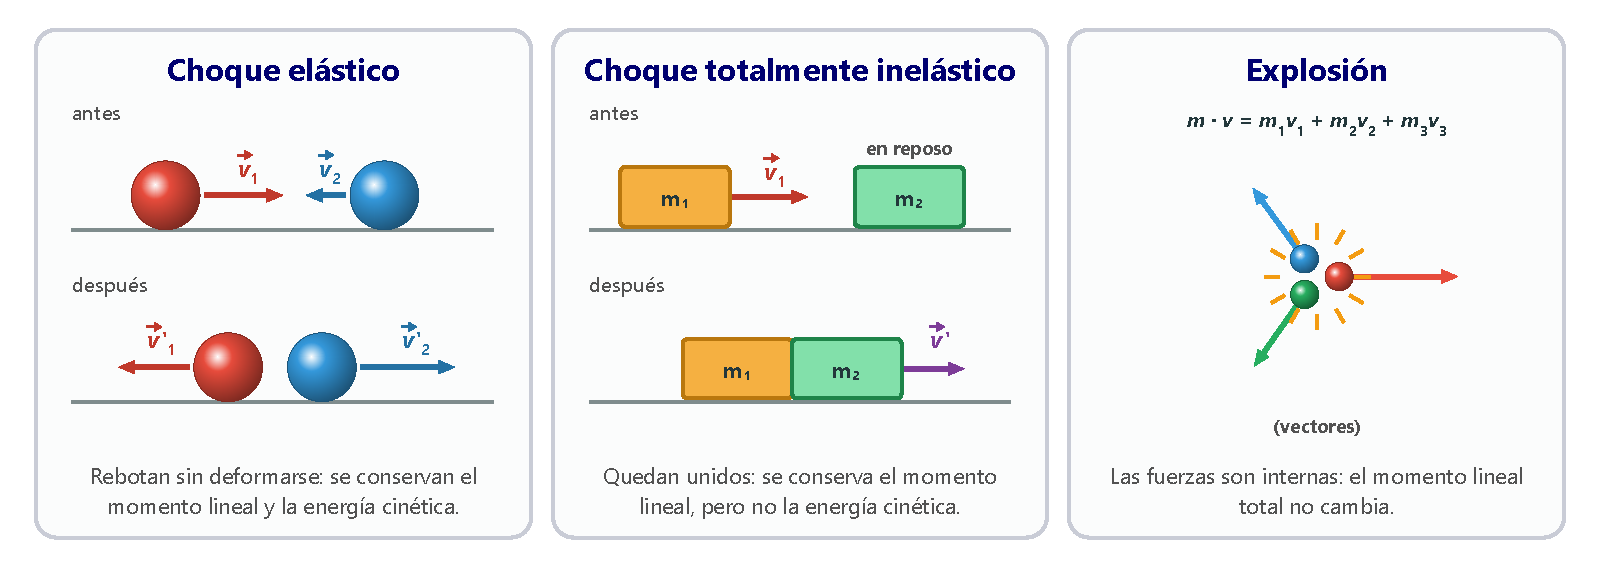
\includegraphics[width=\textwidth]{images/UD10/choques}
    \caption{En choques y explosiones el momento lineal total del sistema se conserva.}
    \label{fig:ud10-choques}
\end{figure}

\begin{example}
    \textbf{Un choque en dos dimensiones.} En una partida de billar, la bola blanca, de \qty{170}{\g}, choca a \qty{3}{\m\per\s} con
    una bola de \qty{160}{\g} en reposo. Tras el choque, esta sale a \qty{2.4}{\m\per\s} formando \(25^\circ\) con la dirección
    inicial de la blanca. ¿Qué velocidad tiene la bola blanca después del choque?

    \textbf{Solución.} Tomamos el eje \(X\) en la dirección inicial de la blanca (A); la otra bola es B.
    \[ \vec{p}_0 = m_A\,\vec{v}_A = \num{0.17} \cdot 3\,\ivec = \num{0.51}\,\ivec~\unit{\kg\m\per\s} \]
    \[ \vec{p}\,'_B = \num{0.16} \cdot (\num{2.4}\cos 25^\circ\,\ivec + \num{2.4}\sen 25^\circ\,\jvec) = (\num{0.348}\,\ivec + \num{0.162}\,\jvec)~\unit{\kg\m\per\s} \]
    Como el momento lineal se conserva, \(\vec{p}_0 = m_A\,\vec{v}\,'_A + \vec{p}\,'_B\):
    \[ \vec{v}\,'_A = \frac{\num{0.51}\,\ivec - (\num{0.348}\,\ivec + \num{0.162}\,\jvec)}{\num{0.17}} = (\num{0.95}\,\ivec - \num{0.95}\,\jvec)~\unit{\m\per\s} \]
    Su módulo es \(\qty{1.35}{\m\per\s}\) y forma \(45^\circ\) por debajo de la dirección inicial.
\end{example}

\begin{exercise}
    Para estudiar el efecto de un disparo, se dispara contra un maniquí de \qty{75}{\kg} en reposo sobre una superficie sin
    rozamiento una bala de \qty{10}{\g}, que se queda incrustada. Si el maniquí adquiere una velocidad de \qty{0.12}{\m\per\s}, ¿cuál
    era la velocidad de la bala?
    \begin{solu}
        \textcolor{blue}{Choque totalmente inelástico: \(m\,v = (m + M)\,v'\).}
        \(v = \dfrac{\num{75.01} \cdot \num{0.12}}{\num{0.010}} = \textcolor{red}{\qty{900}{\m\per\s}}\).
    \end{solu}
\end{exercise}

\begin{exercise}
    Un murciélago de \qty{12}{\g} vuela a \qty{8}{\m\per\s} y caza un insecto de \qty{0.5}{\g} que vuela a \qty{1}{\m\per\s} en la
    misma dirección y sentido. ¿Qué velocidad tiene el murciélago justo después de atraparlo?
    \begin{solu}
        \(v' = \dfrac{\num{0.012} \cdot 8 + \num{0.0005} \cdot 1}{\num{0.0125}} = \textcolor{red}{\qty{7.72}{\m\per\s}}\).
    \end{solu}
\end{exercise}

\begin{exercise}
    En un espectáculo de fuegos artificiales, un cohete de \qty{900}{\g} sube verticalmente y, cuando va a \qty{25}{\m\per\s},
    explota en tres trozos. Un trozo de \qty{300}{\g} sigue subiendo a \qty{40}{\m\per\s}; otro de \qty{250}{\g} sale horizontalmente
    hacia la derecha a \qty{30}{\m\per\s}. Calcula la velocidad del tercer trozo.
    \begin{solu}
        \textcolor{blue}{\(\vec{p} = \num{0.9} \cdot 25\,\jvec = \num{22.5}\,\jvec\); \(\vec{p}_1 = 12\,\jvec\);
        \(\vec{p}_2 = \num{7.5}\,\ivec\); \(\vec{p}_3 = \vec{p} - \vec{p}_1 - \vec{p}_2 = -\num{7.5}\,\ivec + \num{10.5}\,\jvec\).}
        \(\vec{v}_3 = \dfrac{\vec{p}_3}{\num{0.35}} = \textcolor{red}{(-\num{21.4}\,\ivec + 30\,\jvec)~\unit{\m\per\s}}\) (módulo
        \qty{36.9}{\m\per\s}).
    \end{solu}
\end{exercise}

%========================================================================================
\section{El momento angular}\label{sec:ud10-momento-angular}
%========================================================================================

En los apartados anteriores hemos estudiado la \textbf{traslación}: las fuerzas cambian la velocidad de un cuerpo y, sin fuerza
exterior neta, el momento lineal se conserva. Para la \textbf{rotación} hemos visto que el momento de una fuerza puede cambiar la
velocidad angular de un cuerpo. ¿Hay una magnitud que desempeñe en los giros el papel del momento lineal? Sí: el \textbf{momento
angular}.

\subsection{Concepto de momento angular}

\begin{definition}[Momento angular o cinético]
    El momento angular de una partícula respecto a un punto O es el producto vectorial de su vector de posición respecto a O por su
    momento lineal:
    \[ \vec{L} = \vec{r} \times \vec{p} = \vec{r} \times m\,\vec{v} \]
    Su unidad en el SI es el \unit{\kg\m\squared\per\s}.
\end{definition}

No es una propiedad del cuerpo solo: depende del punto O que se elija. Sus características son (figura~\ref{fig:ud10-angular}):
\begin{itemize}
    \item \textbf{Módulo}: \(L = r\,p\sen\alpha = r\,m\,v\sen\alpha\), donde \(\alpha\) es el ángulo entre \(\vec{r}\) y \(\vec{p}\).
    \item \textbf{Dirección}: perpendicular al plano que forman \(\vec{r}\) y \(\vec{p}\).
    \item \textbf{Sentido}: el que da la \textbf{regla de la mano derecha}: si los dedos de la mano derecha giran de \(\vec{r}\) hacia
    \(\vec{p}\) por el camino más corto, el pulgar indica el sentido de \(\vec{L}\). Es también el sentido en que avanza un sacacorchos
    que gira como la partícula.
\end{itemize}
Si \(\vec{r}\) y \(\vec{p}\) tienen la misma dirección (\(\alpha = 0^\circ\) o \(180^\circ\)), el momento angular es nulo. En un
\textbf{movimiento circular} respecto al centro, \(\vec{r}\) y \(\vec{v}\) son siempre perpendiculares y, como \(v = \omega\,r\),
\[ L = m\,v\,r = m\,\omega\,r^2 \]

\begin{figure}[H]
    \centering
    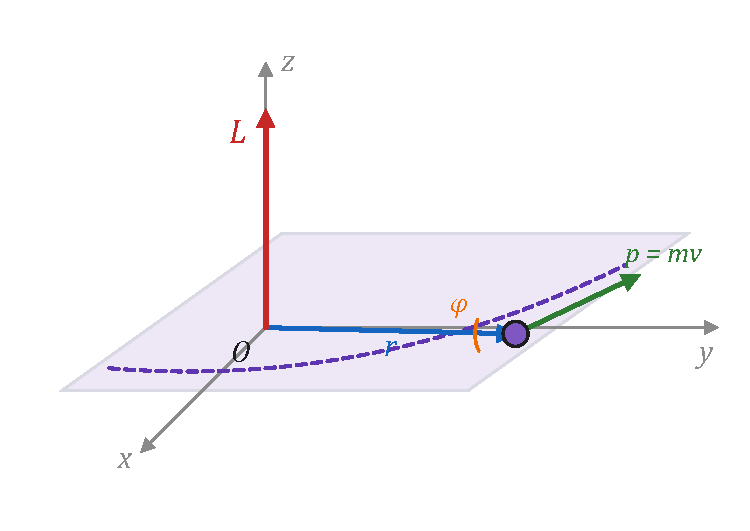
\includegraphics[width=0.55\textwidth]{images/UD10/momento_angular}
    \caption{Momento angular de una partícula respecto a O: perpendicular al plano que forman \(\vec{r}\) y \(\vec{p}\).}
    \label{fig:ud10-angular}
\end{figure}

\begin{example}
    \textbf{En el tiovivo.} Un niño de \qty{25}{\kg} va montado en un tiovivo a \qty{3}{\m} del eje, que gira a \qty{6}{rpm}. Calcula
    su momento angular respecto al eje.

    \textbf{Solución.} \(\omega = 6 \cdot \dfrac{2\pi}{60} = \qty{0.628}{\radian\per\s}\). Como \(\vec{r}\) y \(\vec{v}\) son perpendiculares:
    \[ L = m\,\omega\,r^2 = 25 \cdot \num{0.628} \cdot 3^2 = \qty{141}{\kg\m\squared\per\s} \]
\end{example}

\subsection{Momento de una fuerza y momento angular}

Igual que la fuerza neta cambia el momento lineal, el momento de la fuerza cambia el momento angular. Derivando \(\vec{L}\) con la
regla del producto:
\[ \frac{\dif\vec{L}}{\dif t} = \frac{\dif\vec{r}}{\dif t} \times \vec{p} + \vec{r} \times \frac{\dif\vec{p}}{\dif t}
= \vec{v} \times m\,\vec{v} + \vec{r} \times \vec{F} = \vec{r} \times \vec{F} \]
porque el producto vectorial de dos vectores paralelos es nulo. Por tanto:
\[ \frac{\dif\vec{L}}{\dif t} = \vec{M} \]
Esta es la \textbf{ecuación fundamental de la dinámica de rotación}: la variación del momento angular por unidad de tiempo es igual
al momento de la fuerza neta.

\subsection{Conservación del momento angular}

\begin{definition}[Principio de conservación del momento angular]
    Si el momento resultante de las fuerzas exteriores respecto a un punto O es nulo, el momento angular respecto a ese punto
    permanece constante:
    \[ \vec{M} = \vec{0} = \frac{\dif\vec{L}}{\dif t} \;\Rightarrow\; \vec{L} = \text{constante} \]
\end{definition}

El momento \(\vec{M} = \vec{r} \times \vec{F}\) es nulo en dos casos:
\begin{itemize}
    \item Cuando la fuerza neta es nula.
    \item Cuando \(\vec{r}\) y \(\vec{F}\) son paralelos. Es lo que ocurre con las \textbf{fuerzas centrales}, cuya dirección pasa siempre
    por un punto fijo, como la fuerza de un muelle o la atracción gravitatoria del Sol sobre los planetas.
\end{itemize}

\paragraph{El movimiento de los planetas.} La fuerza con que el Sol atrae a la Tierra es central: está dirigida siempre hacia el Sol
y es paralela al vector de posición. Por eso el momento angular de la Tierra respecto al Sol es constante, y de ahí se deducen dos
cosas: la \textbf{trayectoria es plana} (la dirección de \(\vec{L}\) no cambia) y el planeta va \textbf{más rápido cuanto más cerca
está del Sol} (\(r\,v\) es constante en los puntos en que \(\vec{r}\) y \(\vec{v}\) son perpendiculares). Lo mismo ocurre con todos los
planetas y satélites.

\begin{remark}
    Una patinadora que gira con los brazos extendidos gira mucho más deprisa al recogerlos: al acercar la masa al eje, disminuye
    \(r\) y, para que \(L\) se mantenga, aumenta la velocidad angular.
\end{remark}

\begin{example}
    \textbf{La órbita de la Luna.} En su punto más cercano a la Tierra (perigeo), a \qty{363300}{\km}, la Luna se mueve a
    \qty{3880}{\km\per\hour}; en el más alejado (apogeo), a \qty{3460}{\km\per\hour}. Calcula la distancia Tierra-Luna en el apogeo.

    \textbf{Solución.} La fuerza que la Tierra ejerce sobre la Luna es central, así que el momento angular se conserva. En el perigeo
    y en el apogeo, \(\vec{r}\) y \(\vec{v}\) son perpendiculares (\(\sen\alpha = 1\)):
    \[ L_p = L_a \Rightarrow r_p\,m\,v_p = r_a\,m\,v_a \Rightarrow r_a = \frac{r_p\,v_p}{v_a} = \frac{363300 \cdot 3880}{3460} = \qty{407400}{\km} \]
    No hace falta conocer la masa de la Luna ni pasar las unidades al SI, porque se simplifican.
\end{example}

\begin{exercise}
    Calcula el momento angular del minutero de un reloj de torre respecto al eje. Supón que su masa, \qty{30}{\kg}, está concentrada
    a \qty{1.2}{\m} del eje.
    \begin{solu}
        \(\omega = \dfrac{2\pi}{3600} = \qty{1.745e-3}{\radian\per\s}\); \(L = m\,\omega\,r^2 = 30 \cdot \num{1.745e-3} \cdot \num{1.2}^2 =
        \textcolor{red}{\qty{7.54e-2}{\kg\m\squared\per\s}}\).
    \end{solu}
\end{exercise}

\begin{exercise}
    En el punto de su órbita más cercano al Sol (perihelio), Marte está a \qty{1.38}{UA} y se mueve a \qty{26.5}{\km\per\s}. En el
    más alejado (afelio), está a \qty{1.67}{UA}. ¿Qué velocidad lleva en el afelio?
    \begin{solu}
        \(v_a = \dfrac{r_p\,v_p}{r_a} = \dfrac{\num{1.38} \cdot \num{26.5}}{\num{1.67}} = \textcolor{red}{\qty{21.9}{\km\per\s}}\).
    \end{solu}
\end{exercise}

%========================================================================================
\section{Física en la vida: el bosón de Higgs y el CERN}\label{sec:ud10-higgs}
%========================================================================================

El 4 de julio de 2012, el \textbf{CERN} (Organización Europea para la Investigación Nuclear), en Ginebra, anunció el descubrimiento de
una partícula buscada durante casi medio siglo: el \textbf{bosón de Higgs}. Según el \textbf{Modelo Estándar}, la teoría que describe las
partículas elementales y tres de las cuatro interacciones fundamentales, este bosón está asociado a un campo que llena todo el
espacio y que es el responsable de que las partículas elementales tengan masa.

El hallazgo se hizo en el \textbf{Gran Colisionador de Hadrones} (LHC), un anillo de \qty{27}{\km} de circunferencia situado a unos
\qty{100}{\m} bajo tierra, en la frontera entre Suiza y Francia. En él, dos haces de protones circulan en sentidos opuestos a una
velocidad muy cercana a la de la luz, guiados por imanes superconductores enfriados a \qty{-271.3}{\celsius}, más fríos que el espacio
exterior. Cuando los protones chocan, su enorme energía se convierte en nuevas partículas.

El bosón de Higgs no se observa directamente, porque se desintegra casi al instante. Lo que se detecta son las partículas en que se
desintegra, y para reconstruir lo ocurrido se aplica la \textbf{conservación del momento lineal} (y de la energía) en cada choque. Los
grandes detectores del LHC (ATLAS, CMS, LHCb y ALICE) son, en cierto modo, enormes cámaras que fotografían choques y explosiones de
partículas. El descubrimiento valió el Premio Nobel de Física de 2013 a \textbf{Peter Higgs} y \textbf{François Englert}, que habían
predicho la partícula en 1964.

En el CERN trabajan miles de científicos de todo el mundo. España es estado miembro desde 1983 y cientos de investigadores, ingenieros
y técnicos españoles participan en sus experimentos; entre ellos, la física \textbf{María José Costa}, elegida en 2024 portavoz (máxima
responsable) de la colaboración ATLAS, uno de los dos grandes detectores que descubrieron el Higgs.

\begin{exercise}
    a) En un choque en el LHC, dos protones de igual masa se mueven en la misma dirección y sentidos opuestos con la misma rapidez.
    ¿Cuál es el momento lineal total antes del choque? ¿Qué podemos decir del momento lineal total de todas las partículas que se
    producen? b) Un núcleo en reposo se desintegra en dos fragmentos de masas \(m\) y \(4m\). Si el ligero sale a
    \qty{1.5e7}{\m\per\s}, ¿qué velocidad tiene el pesado? c) Investigad qué otras partículas se han descubierto en aceleradores y
    en qué consisten los cuatro grandes experimentos del LHC.
    \begin{solu}
        a) \(\vec{p} = m\,\vec{v} + m\,(-\vec{v}) = \textcolor{red}{\vec{0}}\); \textcolor{red}{la suma vectorial de los momentos de
        todas las partículas producidas también debe ser nula}. b) \(0 = m \cdot \num{1.5e7} + 4m\,v \Rightarrow
        \textcolor{red}{v = \qty{-3.75e6}{\m\per\s}}\) (en sentido contrario). c) \textcolor{red}{Respuesta abierta} (por ejemplo,
        los bosones W y Z, el quark top, el antiprotón).
    \end{solu}
\end{exercise}

%========================================================================================
\section{Prácticas}\label{sec:ud10-practicas}
%========================================================================================

\subsection{Las tres leyes de la dinámica en casa}

\noindent\begin{minipage}[t]{0.48\textwidth}
    \textbf{Objetivo}
    \begin{itemize}
        \item Comprobar las tres leyes de Newton con materiales caseros.
    \end{itemize}
\end{minipage}\hfill
\begin{minipage}[t]{0.48\textwidth}
    \textbf{Material}
    \begin{itemize}
        \item Un vaso, una cartulina, una moneda, un coche de juguete, una cuerda, unos bloques o piezas de construcción, una pajita, un
        globo y cinta adhesiva.
    \end{itemize}
\end{minipage}

\textbf{Procedimiento}
\begin{enumerate}[label=\numberballgreen]
    \item \textbf{Primera ley.} Tapa el vaso con la cartulina y pon la moneda encima, sobre la boca del vaso. Da un golpe seco y
    horizontal a la cartulina con el dedo: la cartulina sale disparada y la moneda cae dentro del vaso.
    \item \textbf{Segunda ley.} Ata el coche de juguete a una cuerda que pase por el borde de una mesa y cuelga del otro extremo unos
    bloques. Al soltarlos, el peso de los bloques acelera el coche. Repite la experiencia con más bloques colgando y, después,
    cargando el coche con más masa, y observa cómo cambia la aceleración.
    \item \textbf{Tercera ley.} Pasa una cuerda larga por la pajita y átala tensa entre dos puntos de una habitación. Infla el globo
    sin cerrarlo, sujétalo con cinta adhesiva a la pajita y suéltalo: el aire sale hacia atrás y el globo avanza hacia delante por la
    cuerda.
\end{enumerate}

\begin{exercise}
    a) ¿Por qué la moneda no sale despedida junto con la cartulina? ¿Qué ocurre si empujas la cartulina despacio? b) En la segunda
    experiencia, ¿qué ocurre con la aceleración si se duplican los bloques que cuelgan? ¿Y si se duplica la masa del coche?
    c) Identifica la acción y la reacción en el globo. ¿Qué le ocurriría al globo si no estuviera en la cuerda?
    \begin{solu}
        a) \textcolor{red}{Por inercia}: el golpe es tan breve que el rozamiento apenas actúa y la moneda sigue en reposo; al quitar la
        cartulina, cae por su peso. Si se empuja despacio, el rozamiento actúa más tiempo y la moneda se mueve con la cartulina.
        b) \textcolor{red}{Aumenta} (aunque no llega a duplicarse, porque también aumenta la masa total que se acelera);
        \textcolor{red}{disminuye}. c) \textcolor{red}{Acción: el globo empuja el aire hacia atrás; reacción: el aire empuja el globo
        hacia delante.} Sin la cuerda, el globo se movería de forma desordenada porque la dirección del chorro cambia continuamente.
    \end{solu}
\end{exercise}

\subsection{La segunda ley con un carrito}

\noindent\begin{minipage}[t]{0.48\textwidth}
    \textbf{Objetivo}
    \begin{itemize}
        \item Medir la aceleración de un carrito arrastrado por una masa que cuelga y compararla con la que predice la segunda ley.
    \end{itemize}
\end{minipage}\hfill
\begin{minipage}[t]{0.48\textwidth}
    \textbf{Material}
    \begin{itemize}
        \item Un carrito de laboratorio (o un coche de juguete con buenas ruedas), una polea, hilo, pesas, una balanza, una cinta
        métrica y un cronómetro (o el móvil para grabar en vídeo).
    \end{itemize}
\end{minipage}

\begin{figure}[H]
    \centering
    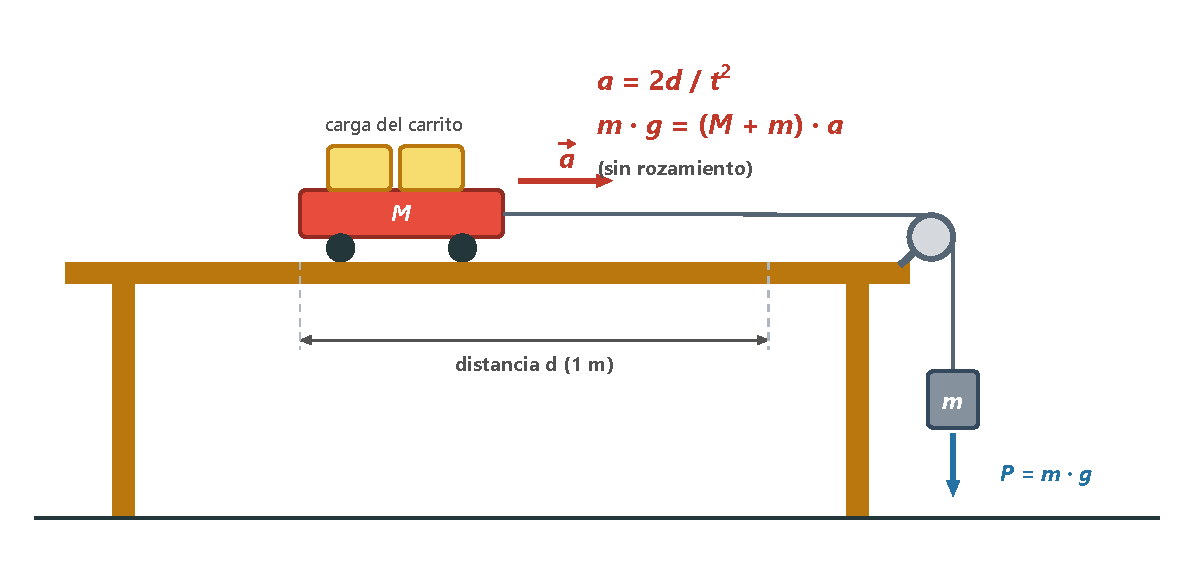
\includegraphics[width=0.75\textwidth]{images/UD10/practica_carrito}
    \caption{El peso de la masa que cuelga acelera todo el sistema: el carrito y la propia masa.}
    \label{fig:ud10-carrito}
\end{figure}

\textbf{Procedimiento}
\begin{enumerate}[label=\numberballgreen]
    \item Mide con la balanza la masa \(M\) del carrito y la masa \(m\) que vas a colgar.
    \item Monta el dispositivo de la figura~\ref{fig:ud10-carrito} y marca en la mesa una distancia \(d = \qty{1}{\m}\).
    \item Suelta el carrito desde el reposo y mide el tiempo \(t\) que tarda en recorrer esa distancia. Repite la medida tres veces y
    calcula el tiempo medio. La aceleración es \(a = 2d/t^2\).
    \item Cambia la masa que cuelga (y luego la carga del carrito) y anota los resultados en una tabla.
\end{enumerate}

\begin{exercise}
    a) Demuestra que, sin rozamiento, la aceleración del sistema es \(a = \dfrac{m\,g}{M + m}\). b) Con \(M = \qty{450}{\g}\) y
    \(m = \qty{50}{\g}\), un grupo mide un tiempo medio de \qty{1.50}{\s} para recorrer \qty{1}{\m}. Calcula la aceleración medida
    y la teórica. c) ¿A qué puede deberse la diferencia? Calcula la fuerza de rozamiento que la explicaría.
    \begin{solu}
        a) \textcolor{blue}{Sobre el sistema (carrito y pesa), la fuerza neta es el peso de la pesa, y la masa que se acelera es la
        total:} \(\textcolor{red}{m\,g = (M + m)\,a}\). b) Medida: \(a = \dfrac{2 \cdot 1}{\num{1.50}^2} =
        \textcolor{red}{\qty{0.89}{\m\per\s\squared}}\); teórica: \(a = \dfrac{\num{0.05} \cdot \num{9.8}}{\num{0.5}} =
        \textcolor{red}{\qty{0.98}{\m\per\s\squared}}\). c) Al \textcolor{red}{rozamiento} (y a los errores al cronometrar):
        \(F_r = m\,g - (M + m)\,a = \num{0.49} - \num{0.5} \cdot \num{0.889} = \textcolor{red}{\qty{0.046}{\newton}}\).
    \end{solu}
\end{exercise}

%========================================================================================
\section{Situación de aprendizaje: cohetes espaciales y cohetes de agua (ODS 9)}\label{sec:ud10-cohetes}
%========================================================================================

Un cohete es un vehículo diseñado para llevar cargas útiles, como satélites, sondas o personas, de la Tierra al espacio. Su
funcionamiento se basa en la \textbf{tercera ley de Newton}: los motores queman una gran cantidad de combustible y expulsan los gases a
gran velocidad hacia abajo; los gases, a su vez, empujan al cohete hacia arriba. Visto de otro modo, es la \textbf{conservación del
momento lineal}: el momento que ganan los gases hacia abajo lo gana el cohete hacia arriba. Los cohetes reutilizables, que aterrizan
para volver a usarse, son un buen ejemplo de la innovación que promueve el \textbf{ODS 9} (industria, innovación e infraestructura).

\begin{marker}
    \textbf{Reto:} por grupos, investigad sobre los cohetes y construid un \textbf{cohete de agua} con materiales reciclados. Grabad un
    vídeo del lanzamiento y preparad un informe que explique su funcionamiento con las leyes de la dinámica.
\end{marker}

\begin{enumerate}[label=\numberballred]
    \item \textbf{Investigad sobre Newton}: su biografía, los científicos que lo inspiraron, sus experimentos y cómo formuló las leyes
    de la dinámica.
    \item \textbf{Investigad sobre los cohetes}: historia y científicos destacados, partes de un cohete, cómo funcionan y cohetes
    actuales y futuros.
    \item \textbf{Relacionad los cohetes con la dinámica}: el empuje y el peso, la velocidad de salida de los gases, la masa del cohete
    y de la carga útil, la velocidad de escape. ¿El empuje tiene que ser mayor que el peso?
    \item \textbf{Construid el cohete de agua} con una botella de plástico, aletas de cartón, agua y una bomba de bicicleta con un tapón
    adaptado. Diseñad la plataforma de lanzamiento, haced un presupuesto y lanzadlo en un lugar despejado y con supervisión.
\end{enumerate}

\begin{exercise}
    a) Un cohete de \qty{2.6e6}{\kg} produce al despegar un empuje de \qty{39}{\mega\newton}. Calcula su aceleración inicial. ¿Qué
    ocurriría si el empuje fuera menor que su peso? b) Un cohete expulsa cada segundo \qty{1200}{\kg} de gases a \qty{3000}{\m\per\s}.
    Calcula el empuje con el teorema del impulso. c) En un cohete de agua de \qty{0.3}{\kg} (vacío), sale \qty{0.5}{\kg} de agua a
    \qty{15}{\m\per\s} en muy poco tiempo. Estima la velocidad que adquiere el cohete (sin tener en cuenta el peso ni el aire).
    \begin{solu}
        a) \(a = \dfrac{F - m\,g}{m} = \dfrac{\num{39e6}}{\num{2.6e6}} - \num{9.8} = \textcolor{red}{\qty{5.2}{\m\per\s\squared}}\).
        \textcolor{red}{Si el empuje fuera menor que el peso, el cohete no despegaría.} b) \(F = \dfrac{\Delta p}{\Delta t} =
        \dfrac{1200 \cdot 3000}{1} = \textcolor{red}{\qty{3.6e6}{\newton}}\). c) Conservación del momento lineal:
        \(\num{0.3}\,v = \num{0.5} \cdot 15 \Rightarrow \textcolor{red}{v = \qty{25}{\m\per\s}}\) (el valor real es menor, porque el
        agua sale poco a poco y actúan el peso y el rozamiento con el aire).
    \end{solu}
\end{exercise}

    \newpage
    %! Unidad 10 — Fundamentos de la dinámica: ejercicios resueltos, ejercicios finales y autoevaluación
%! Fuente: Fuentes/Fisica/Unidad 10 («Ejercicios resueltos», «Practica y calcula», «Piensa y resuelve») y Unidad 11 (captura 425:
%! «Autoevaluación» de este tema; la fuente no trae olimpiadas en esta unidad). Enunciados adaptados con datos cambiados (y más
%! realistas cuando los de la fuente no lo eran: tiempos de contacto, velocidades de proyectiles, cohetes); soluciones rehechas
%! con g = 9,8 m/s². Dificultad: \(\star\) baja, \(\star\star\) media, \(\star\star\star\) alta.

\section{Ejercicios resueltos}\label{sec:ud10-resueltos}

\begin{example}
    \textbf{Choque totalmente inelástico.} Dos bloques de conglomerado se mueven por un carril en la misma dirección y chocan
    quedando unidos. El bloque 1 tiene \qty{1.5}{\kg} y una velocidad de \qty{12}{\m\per\s}; el bloque 2, \qty{2.0}{\kg} y
    \qty{14}{\m\per\s}. Calcula la velocidad de los bloques después del choque: a) si se movían en sentidos contrarios; b) si se
    movían en el mismo sentido (el bloque 2 alcanza al 1).

    \textbf{Solución.} \textbf{1. Datos}: \(m_1 = \qty{1.5}{\kg}\), \(m_2 = \qty{2.0}{\kg}\); tomamos el eje \(X\) en la dirección del
    movimiento, positivo en el sentido del bloque 1. \textbf{Incógnita}: la velocidad común \(\vec{v}\,'\) después del choque.

    \textbf{2. Planteamiento}: en el choque se conserva el momento lineal, \(m_1\,\vec{v}_1 + m_2\,\vec{v}_2 = (m_1 + m_2)\,\vec{v}\,'\).

    \textbf{3. a)} \(\vec{v}_1 = 12\,\ivec\) y \(\vec{v}_2 = -14\,\ivec\)~\unit{\m\per\s}:
    \[ \vec{v}\,' = \frac{\num{1.5} \cdot 12\,\ivec + 2 \cdot (-14)\,\ivec}{\num{3.5}} = -\num{2.86}\,\ivec~\unit{\m\per\s} \]
    Tras el choque los dos se mueven en el sentido en que iba el bloque 2, que tenía más momento lineal (\qty{28}{\kg\m\per\s}
    frente a \qty{18}{\kg\m\per\s}). Comprobación: \(\Delta p_1 = \num{1.5} \cdot (\num{-2.86} - 12) = \qty{-22.3}{\kg\m\per\s}\) y
    \(\Delta p_2 = 2 \cdot (\num{-2.86} + 14) = \qty{+22.3}{\kg\m\per\s}\): lo que pierde uno lo gana el otro.

    \textbf{4. b)} Ahora \(\vec{v}_2 = 14\,\ivec\)~\unit{\m\per\s}:
    \(\vec{v}\,' = \dfrac{\num{1.5} \cdot 12 + 2 \cdot 14}{\num{3.5}}\,\ivec = \num{13.1}\,\ivec~\unit{\m\per\s}\). El bloque 1 gana
    momento lineal y el bloque 2 pierde la misma cantidad.
\end{example}

\begin{example}
    \textbf{Equilibrio: en la tirolina.} En un parque de multiaventura, un alumno de \qty{62}{\kg} se queda colgado de una cuerda
    que forma en ese punto ángulos de \(14^\circ\) y \(6^\circ\) con la horizontal. Dibuja las fuerzas y calcula la tensión de cada
    tramo de la cuerda.

    \textbf{Solución.} \textbf{1. Datos}: \(m = \qty{62}{\kg}\), \(P = 62 \cdot \num{9.8} = \qty{607.6}{\newton}\);
    \(\alpha_1 = 14^\circ\), \(\alpha_2 = 6^\circ\). \textbf{Incógnitas}: \(T_1\) y \(T_2\).

    \textbf{2. Fuerzas}: el peso (vertical hacia abajo) y las dos tensiones, dirigidas a lo largo de la cuerda (como en la
    figura~\ref{fig:ud10-cuerda}). El alumno está en equilibrio: \(\sum F_x = 0\) y \(\sum F_y = 0\).

    \textbf{3. Eje \(X\)}: \(T_2\cos 6^\circ = T_1\cos 14^\circ \Rightarrow T_2 = \dfrac{\cos 14^\circ}{\cos 6^\circ}\,T_1 = \num{0.9756}\,T_1\).

    \textbf{4. Eje \(Y\)}: \(T_1\sen 14^\circ + T_2\sen 6^\circ = P \Rightarrow T_1\,(\num{0.2419} + \num{0.9756} \cdot \num{0.1045}) = \num{607.6}\)
    \[ T_1 = \frac{\num{607.6}}{\num{0.3439}} = \qty{1767}{\newton} \qquad T_2 = \num{0.9756} \cdot 1767 = \qty{1724}{\newton} \]
    Las tensiones son casi tres veces el peso del alumno: por eso las cuerdas de las tirolinas son tan resistentes.
\end{example}

\begin{example}
    \textbf{Segunda ley en un plano inclinado.} Un operario sube un mueble de \qty{40}{\kg} a un camión por una rampa inclinada
    \(20^\circ\), empujándolo con una fuerza de \qty{300}{\newton} paralela a la rampa. La fuerza de rozamiento es de \qty{70}{\newton}.
    a) Dibuja las fuerzas que actúan sobre el mueble. b) Calcula su aceleración.

    \textbf{Solución.} \textbf{1.} Sobre el mueble actúan el peso \(\vec{P}\), la normal \(\vec{N}\), la fuerza del operario
    \(\vec{F}\) (hacia arriba de la rampa) y el rozamiento \(\vec{F}_r\) (hacia abajo, porque se opone al movimiento).

    \textbf{2.} Ejes paralelo y perpendicular a la rampa: \(P = 40 \cdot \num{9.8} = \qty{392}{\newton}\);
    \(P_x = 392\sen 20^\circ = \qty{134.1}{\newton}\); \(P_y = 392\cos 20^\circ = \qty{368.4}{\newton} = N\).

    \textbf{3.} En la dirección del movimiento: \(F - P_x - F_r = m\,a\)
    \[ a = \frac{300 - \num{134.1} - 70}{40} = \qty{2.40}{\m\per\s\squared} \]
\end{example}

\begin{example}
    \textbf{Una explosión en el plano.} Un petardo de \qty{300}{\g} explota cuando su velocidad es
    \(\vec{v}_0 = (20\,\ivec + 15\,\jvec)\)~\unit{\m\per\s} y se divide en dos trozos. Uno, de \qty{120}{\g}, sale con una velocidad
    \(\vec{v}_1 = (35\,\ivec - 40\,\jvec)\)~\unit{\m\per\s}. Calcula la velocidad del otro trozo.

    \textbf{Solución.} \textbf{1.} Las fuerzas de la explosión son internas: el momento lineal se conserva,
    \(m\,\vec{v}_0 = m_1\,\vec{v}_1 + m_2\,\vec{v}_2\), con \(m_2 = 300 - 120 = \qty{180}{\g}\).

    \textbf{2.} \(m\,\vec{v}_0 = \num{0.3} \cdot (20\,\ivec + 15\,\jvec) = (6\,\ivec + \num{4.5}\,\jvec)\)~\unit{\kg\m\per\s};
    \(m_1\,\vec{v}_1 = \num{0.12} \cdot (35\,\ivec - 40\,\jvec) = (\num{4.2}\,\ivec - \num{4.8}\,\jvec)\)~\unit{\kg\m\per\s}.

    \textbf{3.} \(\vec{v}_2 = \dfrac{(6 - \num{4.2})\,\ivec + (\num{4.5} + \num{4.8})\,\jvec}{\num{0.18}} = (10\,\ivec + \num{51.7}\,\jvec)~\unit{\m\per\s}\),
    de módulo \(\sqrt{10^2 + \num{51.7}^2} = \qty{52.7}{\m\per\s}\).
\end{example}

\begin{example}
    \textbf{Un choque en curling.} En un lanzamiento de curling, una piedra de \qty{20}{\kg} que se mueve a \qty{2.2}{\m\per\s}
    choca con otra igual en reposo. Después del choque, las piedras salen formando ángulos de \(30^\circ\) y \(60^\circ\) con la
    dirección inicial, a uno y otro lado de ella. Calcula sus velocidades.

    \textbf{Solución.} \textbf{1.} Eje \(X\) en la dirección inicial. Como las masas son iguales, se simplifican en la conservación del
    momento lineal: \(\vec{v} = \vec{v}_1 + \vec{v}_2\).

    \textbf{2.} Eje \(X\): \(\num{2.2} = v_1\cos 30^\circ + v_2\cos 60^\circ\). Eje \(Y\): \(0 = v_1\sen 30^\circ - v_2\sen 60^\circ\).

    \textbf{3.} De la segunda, \(v_1 = v_2\,\dfrac{\sen 60^\circ}{\sen 30^\circ} = \num{1.732}\,v_2\). Sustituyendo en la primera:
    \(\num{2.2} = v_2\,(\num{1.732} \cdot \num{0.866} + \num{0.5}) = 2\,v_2\), así que \(v_2 = \qty{1.1}{\m\per\s}\) y
    \(v_1 = \qty{1.91}{\m\per\s}\).
\end{example}

%========================================================================================
\section{Ejercicios de aplicación}\label{sec:ud10-aplicacion}
%========================================================================================

\subsection{Las fuerzas}

\begin{exercise}
    \(\star\) Define con tus palabras el concepto de fuerza y clasifica las fuerzas: a) según la proximidad de los cuerpos que
    interaccionan; b) según las interacciones fundamentales de la naturaleza.
    \begin{solu}
        \textcolor{red}{Fuerza: interacción entre dos cuerpos capaz de cambiar su estado de movimiento o de deformarlos.}
        a) \textcolor{red}{De contacto y a distancia.} b) \textcolor{red}{Nuclear fuerte, nuclear débil, electromagnética y
        gravitatoria.}
    \end{solu}
\end{exercise}

\begin{exercise}
    \(\star\) Explica por qué la fuerza es una magnitud vectorial. ¿Qué elementos tiene?
    \begin{solu}
        Porque su efecto depende de hacia dónde y dónde se aplica, no solo de su intensidad. \textcolor{red}{Módulo, dirección,
        sentido y punto de aplicación.}
    \end{solu}
\end{exercise}

\begin{exercise}
    \(\star\) Clasifica estas fuerzas en fuerzas de contacto o a distancia: a) una alumna arrastra una silla; b) un profesor mueve
    un trozo de hierro con un imán sin tocarlo; c) Saturno atrae a su satélite Titán; d) suena el timbre del recreo (el aire empuja
    el tímpano); e) un jugador de baloncesto lanza a canasta.
    \begin{solu}
        \textcolor{red}{De contacto: a, d y e. A distancia: b y c.}
    \end{solu}
\end{exercise}

\begin{exercise}
    \(\star\star\) ¿Qué interacción fundamental actúa en cada caso? a) Una hoja de papel cae desde un segundo piso. b) En el Sol se
    funden núcleos de hidrógeno. c) Los quarks de un protón permanecen unidos. d) Un imán desvía la aguja de una brújula. e) Un
    núcleo de uranio-238 se transforma en torio-234 emitiendo una partícula alfa. f) Se producen las mareas. g) Un paciente se hace
    una resonancia magnética.
    \begin{solu}
        a) \textcolor{red}{Gravitatoria} (y electromagnética en el rozamiento con el aire). b) \textcolor{red}{Nuclear fuerte}
        (y débil). c) \textcolor{red}{Nuclear fuerte}. d) \textcolor{red}{Electromagnética}. e) \textcolor{red}{Nuclear fuerte} (y
        electromagnética, que expulsa la partícula alfa). f) \textcolor{red}{Gravitatoria}. g) \textcolor{red}{Electromagnética}.
    \end{solu}
\end{exercise}

\begin{exercise}
    \(\star\star\) Un muelle mide \qty{12}{\cm} y, al colgarle un peso de \qty{3}{\newton}, pasa a medir \qty{15}{\cm}. a) Calcula su
    constante elástica. b) ¿Cuánto medirá si se le cuelgan \qty{5}{\newton}?
    \begin{solu}
        a) \(k = \dfrac{3}{\num{0.03}} = \textcolor{red}{\qty{100}{\newton\per\m}}\). b) \(\Delta L = \dfrac{5}{100} = \qty{0.05}{\m}\):
        \(L = \textcolor{red}{\qty{17}{\cm}}\).
    \end{solu}
\end{exercise}

\subsection{Componer y descomponer fuerzas}

\begin{exercise}
    \(\star\star\) Mi perro se ha hecho daño en una pata y lo llevo al veterinario en una carretilla de la que tiro con una cuerda,
    aplicando una fuerza de \qty{600}{\newton} que forma \(30^\circ\) con la horizontal. Calcula las componentes horizontal y vertical
    de la fuerza.
    \begin{solu}
        \(F_x = 600\cos 30^\circ = \textcolor{red}{\qty{520}{\newton}}\); \(F_y = 600\sen 30^\circ = \textcolor{red}{\qty{300}{\newton}}\).
    \end{solu}
\end{exercise}

\begin{exercise}
    \(\star\star\) La resultante de dos fuerzas perpendiculares es de \qty{17}{\newton}. Si una de ellas mide \qty{8}{\newton},
    ¿cuánto mide la otra?
    \begin{solu}
        \(F_2 = \sqrt{17^2 - 8^2} = \textcolor{red}{\qty{15}{\newton}}\).
    \end{solu}
\end{exercise}

\begin{exercise}
    \(\star\star\) Sobre un cuerpo actúan cuatro fuerzas en las direcciones de los puntos cardinales: \qty{15}{\newton} hacia el este,
    \qty{9}{\newton} hacia el oeste, \qty{6}{\newton} hacia el norte y \qty{14}{\newton} hacia el sur. Dibújalas y calcula el módulo,
    la dirección y el sentido de la resultante.
    \begin{solu}
        \textcolor{blue}{Este = \(+X\), norte = \(+Y\): \(\vec{F} = (15 - 9)\,\ivec + (6 - 14)\,\jvec = 6\,\ivec - 8\,\jvec\).}
        \(F = \textcolor{red}{\qty{10}{\newton}}\), \textcolor{red}{hacia el sureste, \(\num{53.1}^\circ\) por debajo del este}
        (\(306{,}9^\circ\)).
    \end{solu}
\end{exercise}

\begin{exercise}
    \(\star\star\) Calcula la resultante de tres fuerzas concurrentes de 20, 12 y \qty{15}{\newton}. Las de 12 y \qty{15}{\newton}
    tienen la misma dirección y sentidos opuestos, y la de \qty{20}{\newton} es perpendicular a ellas.
    \begin{solu}
        \(F = \sqrt{20^2 + (15 - 12)^2} = \textcolor{red}{\qty{20.2}{\newton}}\).
    \end{solu}
\end{exercise}

\begin{exercise}
    \(\star\star\) Dos personas empujan un armario. Cuando empujan en la misma dirección y sentido, la resultante es de
    \qty{400}{\newton}; cuando, por error, empujan en sentidos contrarios, es de \qty{90}{\newton}. ¿Qué fuerza hace cada una?
    \begin{solu}
        \textcolor{blue}{\(F_1 + F_2 = 400\) y \(F_1 - F_2 = 90\).} \(\textcolor{red}{F_1 = \qty{245}{\newton}}\) y
        \(\textcolor{red}{F_2 = \qty{155}{\newton}}\).
    \end{solu}
\end{exercise}

\begin{exercise}
    \(\star\star\) Un caballo tira de un carro con una fuerza de \qty{2800}{\newton} que forma \(30^\circ\) con la horizontal. ¿Qué
    parte de esa fuerza actúa en la dirección del movimiento?
    \begin{solu}
        \(F_x = 2800\cos 30^\circ = \textcolor{red}{\qty{2425}{\newton}}\).
    \end{solu}
\end{exercise}

\begin{exercise}
    \(\star\star\) Para devolver a la corriente un tronco varado en un río, dos personas, una en cada orilla, tiran de él con cuerdas
    perpendiculares entre sí con fuerzas de \qty{80}{\newton} y \qty{95}{\newton}. Calcula la fuerza total y el ángulo que forma con
    la primera cuerda.
    \begin{solu}
        \(F = \sqrt{80^2 + 95^2} = \textcolor{red}{\qty{124}{\newton}}\); \(\tg\varphi = \dfrac{95}{80} \Rightarrow
        \textcolor{red}{\varphi = \num{49.9}^\circ}\).
    \end{solu}
\end{exercise}

\begin{exercise}
    \(\star\star\) Calcula la resultante de dos fuerzas de \qty{50}{\newton} y \qty{30}{\newton} que forman un ángulo de \(40^\circ\).
    \begin{solu}
        \(F = \sqrt{50^2 + 30^2 + 2 \cdot 50 \cdot 30\cos 40^\circ} = \textcolor{red}{\qty{75.5}{\newton}}\).
    \end{solu}
\end{exercise}

\begin{exercise}
    \(\star\star\) Calcula la fuerza resultante en cada caso (ejes \(X\) horizontal e \(Y\) vertical):
    a) \(\vec{F}_1 = -4\,\ivec\), \(\vec{F}_2 = -1\,\ivec\), \(\vec{F}_3 = 7\,\ivec\)~N.
    b) \(\vec{F}_1\) de \qty{10}{\newton} a \(45^\circ\) sobre la horizontal, \(\vec{F}_2 = -5\,\ivec\)~N y \(\vec{F}_3 = -6\,\jvec\)~N.
    c) \(\vec{F}_1 = 8\,\jvec\), \(\vec{F}_2 = -12\,\jvec\), \(\vec{F}_3 = 5\,\ivec\), \(\vec{F}_4 = -2\,\ivec\)~N.
    \begin{solu}
        a) \(\vec{F} = 2\,\ivec\)~N: \(\textcolor{red}{\qty{2}{\newton}}\). b) \(\vec{F} = (\num{7.07} - 5)\,\ivec + (\num{7.07} - 6)\,\jvec
        = \num{2.07}\,\ivec + \num{1.07}\,\jvec\): \(\textcolor{red}{\qty{2.33}{\newton}}\). c) \(\vec{F} = 3\,\ivec - 4\,\jvec\):
        \(\textcolor{red}{\qty{5}{\newton}}\).
    \end{solu}
\end{exercise}

\subsection{El equilibrio}

\begin{exercise}
    \(\star\star\) Para secar un vestido de \qty{450}{\g} sin que se arrugue, lo colgamos de una percha en una cuerda, que forma con
    la horizontal ángulos de \(15^\circ\) y \(8^\circ\) a cada lado de la percha. Calcula la tensión de cada tramo de la cuerda.
    \begin{solu}
        \textcolor{blue}{\(T_2 = \num{0.9754}\,T_1\); \(T_1\,(\sen 15^\circ + \num{0.9754}\sen 8^\circ) = \num{0.45} \cdot \num{9.8}\).}
        \(\textcolor{red}{T_1 = \qty{11.2}{\newton}}\) y \(\textcolor{red}{T_2 = \qty{10.9}{\newton}}\).
    \end{solu}
\end{exercise}

\begin{exercise}
    \(\star\star\) Una farola tiene un brazo horizontal del que cuelga una lámpara de \qty{5}{\kg}. El extremo del brazo está sujeto
    también por un cable diagonal que forma \(30^\circ\) con el brazo. Calcula la tensión del cable y la fuerza que soporta el brazo.
    \begin{solu}
        \textcolor{blue}{Vertical: \(T\sen 30^\circ = m\,g\); horizontal: el brazo compensa \(T\cos 30^\circ\).}
        \(T = \dfrac{49}{\num{0.5}} = \textcolor{red}{\qty{98}{\newton}}\); brazo: \(98\cos 30^\circ = \textcolor{red}{\qty{84.9}{\newton}}\)
        (de compresión).
    \end{solu}
\end{exercise}

\begin{exercise}
    \(\star\star\) Queremos colgar una lámpara de \qty{1.6}{\kg} de dos cables iguales que forman entre sí un ángulo de \(50^\circ\).
    ¿Qué tensión soporta cada cable?
    \begin{solu}
        \textcolor{blue}{Cada cable forma \(25^\circ\) con la vertical: \(2T\cos 25^\circ = m\,g\).}
        \(T = \dfrac{\num{15.68}}{2\cos 25^\circ} = \textcolor{red}{\qty{8.65}{\newton}}\).
    \end{solu}
\end{exercise}

\begin{exercise}
    \(\star\star\) Para aflojar el tornillo de la rueda de una avioneta hace falta un momento de \qty{110}{\newton\metre}. ¿Qué fuerza
    perpendicular hay que aplicar con una llave de \qty{30}{\cm}?
    \begin{solu}
        \(F = \dfrac{M}{r} = \dfrac{110}{\num{0.30}} = \textcolor{red}{\qty{367}{\newton}}\).
    \end{solu}
\end{exercise}

\begin{exercise}
    \(\star\star\) Dos personas llevan un saco de arroz de \qty{150}{\kg} colgado de una barra de \qty{2}{\m} de peso despreciable.
    Si una aguanta 1,5 veces más peso que la otra, ¿qué fuerza hace cada una y dónde está colgado el saco?
    \begin{solu}
        \textcolor{blue}{\(F_1 + F_2 = 1470\) y \(F_1 = \num{1.5}\,F_2\); momentos respecto al saco: \(F_1\,d_1 = F_2\,d_2\).}
        \(\textcolor{red}{F_2 = \qty{588}{\newton}}\), \(\textcolor{red}{F_1 = \qty{882}{\newton}}\); \(d_1 = \dfrac{2 \cdot 588}{1470} =
        \textcolor{red}{\qty{0.8}{\m}}\) de la persona que soporta más peso.
    \end{solu}
\end{exercise}

\begin{exercise}
    \(\star\star\) En muchos países se transportan cargas colgadas de los extremos de una barra que se apoya en el hombro. Si una
    persona lleva cubos de agua de \qty{5}{\kg} y \qty{8}{\kg} en los extremos de una barra de \qty{1.5}{\m}, ¿qué fuerza hace y en
    qué punto de la barra debe apoyarla?
    \begin{solu}
        \(F = 13 \cdot \num{9.8} = \textcolor{red}{\qty{127.4}{\newton}}\); \(5\,x = 8\,(\num{1.5} - x) \Rightarrow
        \textcolor{red}{x = \qty{0.92}{\m}}\) del cubo de \qty{5}{\kg}.
    \end{solu}
\end{exercise}

\begin{exercise}
    \(\star\star\) Dos pintores transportan una escalera de \qty{5}{\m} y \qty{25}{\kg}. Uno la sujeta por un extremo y el otro a
    \qty{60}{\cm} del otro extremo. ¿Qué fuerza hace cada uno?
    \begin{solu}
        \textcolor{blue}{Momentos respecto al primero: \(F_B \cdot \num{4.4} = 245 \cdot \num{2.5}\).}
        \(\textcolor{red}{F_B = \qty{139}{\newton}}\) y \(\textcolor{red}{F_A = 245 - 139 = \qty{106}{\newton}}\).
    \end{solu}
\end{exercise}

\begin{exercise}
    \(\star\star\) En un balancín, un niño de \qty{30}{\kg} se sienta a \qty{1.6}{\m} del eje. ¿Dónde debe sentarse su hermana, de
    \qty{40}{\kg}, para que el balancín quede en equilibrio horizontal?
    \begin{solu}
        \(30 \cdot \num{1.6} = 40\,x \Rightarrow \textcolor{red}{x = \qty{1.2}{\m}}\) del eje, al otro lado.
    \end{solu}
\end{exercise}

\subsection{Las leyes de Newton}

\begin{exercise}
    \(\star\) Explica con tus palabras qué es la inercia y pon un ejemplo de la vida cotidiana en el que se manifieste.
    \begin{solu}
        \textcolor{red}{Es la tendencia de los cuerpos a mantener su estado de reposo o de MRU.} Ejemplo: al arrancar un autobús, los
        pasajeros de pie se van hacia atrás.
    \end{solu}
\end{exercise}

\begin{exercise}
    \(\star\) ¿Son verdaderas estas afirmaciones? Corrige las falsas. a) Si sobre un cuerpo actúa una sola fuerza, la resultante es
    cero. b) La masa de un cuerpo no influye en su movimiento. c) La fuerza de rozamiento sobre el hielo se opone muy poco al
    movimiento. d) Para que un cuerpo en reposo empiece a moverse no hace falta aplicarle una fuerza. e) Una fuerza constante puede
    hacer que un cuerpo lleve un MRUA.
    \begin{solu}
        a) \textcolor{red}{F}: la resultante es esa fuerza. b) \textcolor{red}{F}: a mayor masa, menor aceleración para la misma fuerza.
        c) \textcolor{red}{V}. d) \textcolor{red}{F}: hace falta una fuerza neta. e) \textcolor{red}{V}.
    \end{solu}
\end{exercise}

\begin{exercise}
    \(\star\star\) Tenemos dos bloques de hierro de \qty{3}{\kg} y \qty{6}{\kg}. ¿Cuáles de estas afirmaciones son verdaderas?
    a) El primero tiene la mitad de inercia que el segundo. b) Si se aplica la misma fuerza neta a ambos, el primero adquiere el doble
    de aceleración. c) Si dejan de actuar las fuerzas sobre los bloques en movimiento, el de mayor masa se moverá durante más tiempo.
    \begin{solu}
        \textcolor{red}{Verdaderas: a y b.} c) es falsa: sin fuerzas, \textcolor{red}{los dos seguirían moviéndose indefinidamente con
        MRU}.
    \end{solu}
\end{exercise}

\begin{exercise}
    \(\star\star\) Sobre un cuerpo de \qty{12}{\kg} que está en un plano horizontal sin rozamiento actúan dos fuerzas de
    \qty{10}{\newton} y \qty{26}{\newton}. Calcula su aceleración si las fuerzas: a) tienen la misma dirección y sentido; b) tienen
    la misma dirección y sentidos contrarios; c) son perpendiculares.
    \begin{solu}
        a) \(a = \dfrac{36}{12} = \textcolor{red}{\qty{3}{\m\per\s\squared}}\). b) \(a = \dfrac{16}{12} = \textcolor{red}{\qty{1.33}{\m\per\s\squared}}\).
        c) \(a = \dfrac{\sqrt{10^2 + 26^2}}{12} = \textcolor{red}{\qty{2.32}{\m\per\s\squared}}\).
    \end{solu}
\end{exercise}

\begin{exercise}
    \(\star\) ¿Por qué un objeto que se desliza por una superficie horizontal acaba parándose? ¿Contradice esto la primera ley?
    \begin{solu}
        Porque actúa sobre él la \textcolor{red}{fuerza de rozamiento}, que lo frena. \textcolor{red}{No la contradice}: la primera
        ley dice que el cuerpo mantendría su velocidad solo si la fuerza neta fuese nula.
    \end{solu}
\end{exercise}

\begin{exercise}
    \(\star\star\) Una caja de \qty{80}{\kg} en reposo se empuja horizontalmente con una fuerza de \qty{280}{\newton}. El
    rozamiento es de \qty{180}{\newton}. ¿Qué velocidad tiene al cabo de \qty{4}{\s}?
    \begin{solu}
        \(a = \dfrac{100}{80} = \qty{1.25}{\m\per\s\squared}\); \(v = \textcolor{red}{\qty{5}{\m\per\s}}\).
    \end{solu}
\end{exercise}

\begin{exercise}
    \(\star\star\) Un trabajador sube un mueble de \qty{45}{\kg} a un camión por una rampa inclinada \(18^\circ\), empujándolo con
    una fuerza de \qty{320}{\newton} paralela a la rampa. El rozamiento es de \qty{60}{\newton}. a) Dibuja las fuerzas. b) ¿Con qué
    aceleración sube?
    \begin{solu}
        \(P_x = 45 \cdot \num{9.8}\sen 18^\circ = \qty{136.3}{\newton}\); b) \(a = \dfrac{320 - 60 - \num{136.3}}{45} =
        \textcolor{red}{\qty{2.75}{\m\per\s\squared}}\).
    \end{solu}
\end{exercise}

\begin{exercise}
    \(\star\star\) Una persona sostiene a un bebé con los brazos extendidos. ¿Cuál es la reacción al peso del bebé? a) La normal que
    el suelo hace sobre los pies de la persona. b) La fuerza que las manos hacen sobre el bebé. c) La fuerza que el bebé hace sobre las
    manos. d) La fuerza gravitatoria con que el bebé atrae a la Tierra.
    \begin{solu}
        \textcolor{red}{d}. El peso es la fuerza con que la Tierra atrae al bebé; su reacción, aplicada en la Tierra, es la fuerza con
        que el bebé atrae a la Tierra. Las manos y el bebé forman otro par de acción y reacción (b y c).
    \end{solu}
\end{exercise}

\begin{exercise}
    \(\star\star\) Un cohete Falcon 9 de \qty{550}{t} despega verticalmente con una aceleración inicial de \qty{4}{\m\per\s\squared}.
    ¿Qué fuerza de empuje producen sus motores?
    \begin{solu}
        \textcolor{blue}{\(F - m\,g = m\,a\).} \(F = \num{550000} \cdot (\num{9.8} + 4) = \textcolor{red}{\qty{7.59e6}{\newton}}\).
    \end{solu}
\end{exercise}

\begin{exercise}
    \(\star\) Explica con la tercera ley de Newton cómo avanza: a) una nadadora; b) una barca de remos; c) un calamar.
    \begin{solu}
        \textcolor{red}{En los tres casos el cuerpo empuja el agua hacia atrás y el agua lo empuja hacia delante con una fuerza igual
        y opuesta}: a) con brazos y piernas; b) con los remos; c) expulsando un chorro de agua.
    \end{solu}
\end{exercise}

\subsection{Momento lineal}

\begin{exercise}
    \(\star\star\) Un patinador de \qty{80}{\kg} (con su monopatín) va a \qty{18}{\km\per\hour} y frena durante \qty{0.8}{\s} hasta
    \qty{7.2}{\km\per\hour}. Calcula: a) la variación de su momento lineal; b) la fuerza media de frenado.
    \begin{solu}
        a) \(\Delta p = 80 \cdot (2 - 5) = \textcolor{red}{\qty{-240}{\kg\m\per\s}}\). b) \(F = \dfrac{-240}{\num{0.8}} =
        \textcolor{red}{\qty{-300}{\newton}}\).
    \end{solu}
\end{exercise}

\begin{exercise}
    \(\star\star\) Una pelota de béisbol de \qty{145}{\g} llega al bate a \qty{90}{\km\per\hour} y sale en sentido contrario a
    \qty{120}{\km\per\hour}. Si el contacto dura \qty{1}{\milli\s}, calcula el impulso y la fuerza media que ejerce el bate.
    \begin{solu}
        \(\Delta v = \num{33.3} + 25 = \qty{58.3}{\m\per\s}\); \(I = \num{0.145} \cdot \num{58.3} = \textcolor{red}{\qty{8.46}{\newton\s}}\);
        \(F = \textcolor{red}{\qty{8.46e3}{\newton}}\), en el sentido de salida.
    \end{solu}
\end{exercise}

\begin{exercise}
    \(\star\star\) En un partido de bádminton, un volante de \qty{5}{\g} llega a la raqueta a \qty{80}{\m\per\s} y sale en sentido
    contrario con la misma rapidez. Si el contacto dura \qty{3}{\milli\s}, ¿qué impulso le da la raqueta? ¿Qué fuerza media hace?
    \begin{solu}
        \(I = \num{0.005} \cdot (-80 - 80) = \textcolor{red}{\qty{-0.8}{\newton\s}}\); \(F = \dfrac{\num{-0.8}}{\num{0.003}} =
        \textcolor{red}{\qty{-267}{\newton}}\) (signo negativo: en sentido contrario al de llegada).
    \end{solu}
\end{exercise}

\begin{exercise}
    \(\star\star\) Un petardo de \qty{400}{\g} explota cuando su velocidad es \(\vec{v}_0 = (30\,\ivec + 20\,\jvec)\)~\unit{\m\per\s}
    y se divide en dos partes. La primera, de \qty{150}{\g}, sale con \(\vec{v}_1 = (40\,\ivec - 30\,\jvec)\)~\unit{\m\per\s}.
    Calcula la velocidad de la otra parte.
    \begin{solu}
        \(\vec{v}_2 = \dfrac{\num{0.4}\,\vec{v}_0 - \num{0.15}\,\vec{v}_1}{\num{0.25}} = \dfrac{(12 - 6)\,\ivec + (8 + \num{4.5})\,\jvec}{\num{0.25}}
        = \textcolor{red}{(24\,\ivec + 50\,\jvec)~\unit{\m\per\s}}\).
    \end{solu}
\end{exercise}

\begin{exercise}
    \(\star\star\) Un astronauta de la Estación Espacial sale al exterior para reparar un panel. Para moverse, sus propulsores expulsan
    \qty{25}{\g} de gas por segundo a \qty{100}{\m\per\s}. Si su masa total es de \qty{200}{\kg}, calcula el impulso que recibe cada
    segundo, la fuerza de empuje y su aceleración.
    \begin{solu}
        \(I = \num{0.025} \cdot 100 = \textcolor{red}{\qty{2.5}{\newton\s}}\) cada segundo; \(F = \textcolor{red}{\qty{2.5}{\newton}}\);
        \(a = \dfrac{\num{2.5}}{200} = \textcolor{red}{\qty{0.0125}{\m\per\s\squared}}\).
    \end{solu}
\end{exercise}

\begin{exercise}
    \(\star\star\) Una gaviota de \qty{1.1}{\kg} vuela con \(\vec{v}_g = (16\,\ivec + 10\,\jvec)\)~\unit{\m\per\s} y atrapa un pájaro
    de \qty{120}{\g} que vuela con \(\vec{v}_p = (12\,\ivec + 6\,\jvec)\)~\unit{\m\per\s}. ¿Qué velocidad tiene la gaviota justo
    después?
    \begin{solu}
        \(\vec{v} = \dfrac{(\num{17.6} + \num{1.44})\,\ivec + (11 + \num{0.72})\,\jvec}{\num{1.22}} = \textcolor{red}{(\num{15.6}\,\ivec + \num{9.61}\,\jvec)~\unit{\m\per\s}}\).
    \end{solu}
\end{exercise}

\begin{exercise}
    \(\star\star\) Un vagón de \qty{12}{t} que se mueve a \qty{2}{\m\per\s} choca con otro de \qty{8}{t} en reposo y quedan
    enganchados. a) ¿Con qué velocidad se mueven después? b) Calcula la energía cinética antes y después. ¿Qué tipo de choque es?
    \begin{solu}
        a) \(v' = \dfrac{12000 \cdot 2}{20000} = \textcolor{red}{\qty{1.2}{\m\per\s}}\). b) \(E_{c,0} = \frac{1}{2} \cdot 12000 \cdot 2^2 =
        \textcolor{red}{\qty{24000}{\joule}}\); \(E_{c,f} = \frac{1}{2} \cdot 20000 \cdot \num{1.2}^2 = \textcolor{red}{\qty{14400}{\joule}}\).
        Se pierde el \qty{40}{\percent}: \textcolor{red}{choque totalmente inelástico}.
    \end{solu}
\end{exercise}

\subsection{Momento angular}

\begin{exercise}
    \(\star\star\) Calcula el momento angular de Venus respecto al Sol, sabiendo que el radio de su órbita (casi circular) es de
    \qty{108.2e6}{\km}, su masa es de \qty{4.87e24}{\kg} y tarda 224,7 días en completarla.
    \begin{solu}
        \(\omega = \dfrac{2\pi}{\num{224.7} \cdot 86400} = \qty{3.24e-7}{\radian\per\s}\); \(L = m\,\omega\,r^2 =
        \textcolor{red}{\qty{1.85e40}{\kg\m\squared\per\s}}\).
    \end{solu}
\end{exercise}

\begin{exercise}
    \(\star\star\) Un disco de vinilo de \qty{15}{\cm} de radio gira a \qty{45}{rpm}. Una mosca de \qty{0.06}{\g} se posa en su borde
    y gira con él. ¿Cuál es su momento angular respecto al eje?
    \begin{solu}
        \(\omega = 45 \cdot \dfrac{2\pi}{60} = \qty{4.71}{\radian\per\s}\); \(L = \num{6e-5} \cdot \num{4.71} \cdot \num{0.15}^2 =
        \textcolor{red}{\qty{6.36e-6}{\kg\m\squared\per\s}}\).
    \end{solu}
\end{exercise}

\begin{exercise}
    \(\star\star\) La Estación Espacial Internacional, de unas \qty{420}{t}, gira alrededor de la Tierra a \qty{7.66}{\km\per\s} a
    \qty{410}{\km} de altura. Calcula su momento angular respecto al centro de la Tierra (\(R_T = \qty{6371}{\km}\)).
    \begin{solu}
        \(L = m\,v\,r = \num{4.2e5} \cdot 7660 \cdot \num{6.781e6} = \textcolor{red}{\qty{2.18e16}{\kg\m\squared\per\s}}\).
    \end{solu}
\end{exercise}

\begin{exercise}
    \(\star\star\) El cometa Halley pasa por el perihelio a \qty{0.586}{UA} del Sol con una velocidad de \qty{54.6}{\km\per\s}. Su
    afelio está a \qty{35.1}{UA}. ¿Qué velocidad lleva allí?
    \begin{solu}
        \(v_a = \dfrac{\num{0.586} \cdot \num{54.6}}{\num{35.1}} = \textcolor{red}{\qty{0.91}{\km\per\s}}\).
    \end{solu}
\end{exercise}

\begin{exercise}
    \(\star\) Explica con la conservación del momento angular por qué una patinadora gira más deprisa al recoger los brazos y por qué
    la órbita de la Tierra es plana.
    \begin{solu}
        \textcolor{red}{Al recoger los brazos, la masa se acerca al eje; como \(L\) se conserva, aumenta la velocidad angular. La
        fuerza del Sol es central, así que \(\vec{L}\) de la Tierra es constante en dirección: la órbita está siempre en el plano
        perpendicular a \(\vec{L}\).}
    \end{solu}
\end{exercise}

%========================================================================================
\section{Ejercicios de ampliación}\label{sec:ud10-ampliacion}
%========================================================================================

\begin{exercise}
    \(\star\star\star\) Haz un trabajo de investigación sobre las ideas de Aristóteles y de Galileo acerca del movimiento y las
    fuerzas. ¿En qué se diferencian de las de Newton?
    \begin{solu}
        \textcolor{red}{Respuesta abierta.} Aristóteles: hace falta una fuerza para mantener el movimiento; Galileo: introduce la
        inercia; Newton: la fuerza causa la aceleración (\(\vec{F} = m\,\vec{a}\)) y las fuerzas son interacciones (acción y reacción).
    \end{solu}
\end{exercise}

\begin{exercise}
    \(\star\star\) Un cuerpo de \qty{90}{\kg} es arrastrado por una superficie horizontal con una fuerza de \qty{700}{\newton}.
    Suponiendo que el rozamiento vale siempre \qty{180}{\newton}, calcula la aceleración cuando la fuerza: a) es horizontal;
    b) forma \(25^\circ\) con la horizontal. Dibuja las fuerzas en ambos casos.
    \begin{solu}
        a) \(a = \dfrac{700 - 180}{90} = \textcolor{red}{\qty{5.78}{\m\per\s\squared}}\). b) \(a = \dfrac{700\cos 25^\circ - 180}{90} =
        \textcolor{red}{\qty{5.05}{\m\per\s\squared}}\). (En realidad, al tirar hacia arriba disminuye la normal y con ella el
        rozamiento; lo estudiaremos en la unidad siguiente.)
    \end{solu}
\end{exercise}

\begin{exercise}
    \(\star\star\star\) Sobre un meteorito de \qty{5}{\kg} que viaja por el espacio actúa durante \qty{12}{\s} una fuerza constante
    \(\vec{F} = (20\,\ivec - 10\,\jvec + 40\,\kvec)\)~N. Si al final su velocidad es \((25\,\ivec + 20\,\jvec - 30\,\kvec)\)~\unit{\m\per\s},
    ¿cuál era su velocidad inicial?
    \begin{solu}
        \textcolor{blue}{\(\vec{F}\,\Delta t = m\,(\vec{v} - \vec{v}_0) \Rightarrow \vec{v}_0 = \vec{v} - \dfrac{\vec{F}\,\Delta t}{m} =
        \vec{v} - (48\,\ivec - 24\,\jvec + 96\,\kvec)\).}
        \(\textcolor{red}{\vec{v}_0 = (-23\,\ivec + 44\,\jvec - 126\,\kvec)~\unit{\m\per\s}}\).
    \end{solu}
\end{exercise}

\begin{exercise}
    \(\star\star\) Una persona de \qty{60}{\kg} está sobre una báscula dentro de un ascensor. ¿Qué marca la báscula (en newtons)
    cuando el ascensor: a) sube con velocidad constante; b) arranca hacia arriba con una aceleración de \qty{1.5}{\m\per\s\squared};
    c) frena al subir con una aceleración de \qty{1.5}{\m\per\s\squared}?
    \begin{solu}
        \textcolor{blue}{La báscula marca la normal: \(N - m\,g = m\,a\).} a) \(N = \textcolor{red}{\qty{588}{\newton}}\).
        b) \(N = 60 \cdot (\num{9.8} + \num{1.5}) = \textcolor{red}{\qty{678}{\newton}}\). c) \(N = 60 \cdot (\num{9.8} - \num{1.5}) =
        \textcolor{red}{\qty{498}{\newton}}\).
    \end{solu}
\end{exercise}

\begin{exercise}
    \(\star\star\star\) Un lanzador de peso sostiene en la mano una bola que pesa \qty{50}{\newton}, con el antebrazo horizontal y
    formando \(90^\circ\) con el brazo. El bíceps se inserta a \qty{4}{\cm} del codo y tira verticalmente hacia arriba; la bola está a
    \qty{32}{\cm} del codo. Despreciando el peso del antebrazo, ¿qué fuerza hace el bíceps?
    \begin{solu}
        \textcolor{blue}{Momentos respecto al codo: \(F \cdot \num{0.04} = 50 \cdot \num{0.32}\).}
        \(F = \textcolor{red}{\qty{400}{\newton}}\): ocho veces el peso de la bola.
    \end{solu}
\end{exercise}

\begin{exercise}
    \(\star\star\star\) Una plataforma de \qty{12}{\m} y \qty{300}{\kg} está colocada sobre el tejado de un edificio, apoyada en su
    borde, de modo que una parte sobresale. Una persona de \qty{700}{\newton} camina por la parte que sobresale hasta el extremo.
    ¿Cuánto puede sobresalir como máximo la plataforma sin que vuelque?
    \begin{solu}
        \textcolor{blue}{Si sobresale \(x\), el peso de la plataforma actúa a \(6 - x\) del borde y la persona a \(x\): \(700\,x = 2940\,(6 - x)\).}
        \(x = \textcolor{red}{\qty{4.85}{\m}}\).
    \end{solu}
\end{exercise}

\begin{exercise}
    \(\star\star\star\) Un jugador despeja un balón de \qty{430}{\g} golpeándolo con una fuerza media de \qty{400}{\newton}. El balón
    sale con un ángulo de \(40^\circ\) y vuelve a tocar el suelo a \qty{45}{\m}. ¿Cuánto duró el golpe?
    \begin{solu}
        \textcolor{blue}{Alcance del tiro parabólico: \(x = \dfrac{v_0^2\sen 2\alpha}{g} \Rightarrow v_0 = \sqrt{\dfrac{45 \cdot \num{9.8}}{\sen 80^\circ}} = \qty{21.2}{\m\per\s}\).}
        \(\Delta t = \dfrac{m\,v_0}{F} = \dfrac{\num{0.43} \cdot \num{21.2}}{400} = \textcolor{red}{\qty{0.023}{\s}}\).
    \end{solu}
\end{exercise}

\begin{exercise}
    \(\star\star\star\) Dos bolas de billar iguales chocan frontalmente de forma elástica. Una iba a \qty{4}{\m\per\s} y la otra
    estaba en reposo. Demuestra, con la conservación del momento lineal y de la energía cinética, que intercambian sus velocidades.
    \begin{solu}
        \textcolor{blue}{\(4 = v_1' + v_2'\) y \(16 = v_1'^2 + v_2'^2\). Elevando la primera al cuadrado y restando, \(v_1'\,v_2' = 0\).}
        La solución con choque es \(\textcolor{red}{v_1' = 0}\) y \(\textcolor{red}{v_2' = \qty{4}{\m\per\s}}\).
    \end{solu}
\end{exercise}

\begin{exercise}
    \(\star\star\star\) Péndulo balístico. Una bala de \qty{8}{\g} se incrusta en un bloque de madera de \qty{2}{\kg} que cuelga de
    unos hilos, y el bloque sube \qty{10}{\cm}. a) ¿Con qué velocidad empezó a moverse el bloque? (Usa la conservación de la energía
    mecánica.) b) ¿Cuál era la velocidad de la bala?
    \begin{solu}
        a) \(V = \sqrt{2\,g\,h} = \textcolor{red}{\qty{1.4}{\m\per\s}}\). b) Choque totalmente inelástico: \(v = \dfrac{\num{2.008} \cdot
        \num{1.4}}{\num{0.008}} = \textcolor{red}{\qty{351}{\m\per\s}}\).
    \end{solu}
\end{exercise}

\begin{exercise}
    \(\star\star\star\) Una piedra atada a una cuerda gira en un plano horizontal sin rozamiento, en una circunferencia de \qty{1}{\m}
    de radio, a 2 vueltas por segundo. La cuerda pasa por un tubo vertical en el centro y tiramos de ella hasta que el radio es de
    \qty{0.5}{\m}. ¿Qué velocidad y qué frecuencia tiene ahora la piedra?
    \begin{solu}
        \textcolor{blue}{La fuerza de la cuerda es central: \(m\,r_1\,v_1 = m\,r_2\,v_2\), con \(v_1 = 2\pi \cdot 1 \cdot 2 = \qty{12.6}{\m\per\s}\).}
        \(v_2 = \textcolor{red}{\qty{25.1}{\m\per\s}}\); \(f = \dfrac{v_2}{2\pi r_2} = \textcolor{red}{8~\text{vueltas/s}}\).
    \end{solu}
\end{exercise}

\begin{exercise}
    \(\star\star\star\) Un coche de \qty{1200}{\kg} a \qty{90}{\km\per\hour} choca de frente con un camión de \qty{8000}{\kg} que
    circula en sentido contrario a \qty{54}{\km\per\hour}, y quedan unidos. a) ¿Con qué velocidad se mueven tras el choque? b) Si el
    choque dura \qty{0.1}{\s}, calcula la aceleración media de los ocupantes del coche y compárala con \(g\). c) ¿Qué fuerza media
    actúa sobre cada vehículo?
    \begin{solu}
        a) \(v' = \dfrac{1200 \cdot 25 - 8000 \cdot 15}{9200} = \textcolor{red}{\qty{-9.78}{\m\per\s}}\) (en el sentido del camión).
        b) \(a = \dfrac{\num{-9.78} - 25}{\num{0.1}} = \textcolor{red}{\qty{-348}{\m\per\s\squared}}\), unas \textcolor{red}{35 veces
        \(g\)}. c) \(F = 1200 \cdot 348 = \textcolor{red}{\qty{4.17e5}{\newton}}\) sobre cada uno (acción y reacción), aunque el
        camión apenas cambia su velocidad.
    \end{solu}
\end{exercise}

\begin{exercise}
    \(\star\star\) Dos patinadores de \qty{60}{\kg} y \qty{75}{\kg} están en reposo sobre el hielo y se empujan. Si el primero sale a
    \qty{1.5}{\m\per\s}, ¿qué velocidad adquiere el segundo? ¿Hacen la misma fuerza los dos?
    \begin{solu}
        \(v_2 = -\dfrac{60 \cdot \num{1.5}}{75} = \textcolor{red}{\qty{-1.2}{\m\per\s}}\) (en sentido contrario).
        \textcolor{red}{Sí}: por la tercera ley, las fuerzas son iguales y opuestas.
    \end{solu}
\end{exercise}

%========================================================================================
\section{Autoevaluación}\label{sec:ud10-autoevaluacion}
%========================================================================================

\begin{exercise}
    ¿Podemos decir que no actúa ninguna fuerza sobre un objeto que se mueve con velocidad constante? Razónalo.
    \begin{solu}
        \textcolor{red}{No}: pueden actuar varias fuerzas, pero su \textcolor{red}{resultante es nula} (primera ley).
    \end{solu}
\end{exercise}

\begin{exercise}
    Clasifica las fuerzas según las interacciones fundamentales de la naturaleza y pon un ejemplo de cada una.
    \begin{solu}
        \textcolor{red}{Nuclear fuerte} (cohesión del núcleo), \textcolor{red}{nuclear débil} (desintegración beta),
        \textcolor{red}{electromagnética} (atracción de un imán) y \textcolor{red}{gravitatoria} (el peso).
    \end{solu}
\end{exercise}

\begin{exercise}
    Explica con tus palabras las tres leyes de la dinámica y pon un ejemplo cotidiano de cada una.
    \begin{solu}
        \textcolor{red}{Inercia} (los pasajeros se van hacia delante al frenar), \textcolor{red}{fundamental} (cuesta más acelerar un
        carro lleno que uno vacío) y \textcolor{red}{acción y reacción} (al caminar empujamos el suelo hacia atrás).
    \end{solu}
\end{exercise}

\begin{exercise}
    Tiramos de un cuerpo con una cuerda que forma \(30^\circ\) con la horizontal, aplicando una fuerza de \qty{250}{\newton}. Calcula
    las componentes horizontal y vertical de la fuerza.
    \begin{solu}
        \(F_x = \textcolor{red}{\qty{216.5}{\newton}}\); \(F_y = \textcolor{red}{\qty{125}{\newton}}\).
    \end{solu}
\end{exercise}

\begin{exercise}
    Ana y Luis transportan en una tabla de \qty{3}{\m} de peso despreciable un cuerpo que pesa \qty{800}{\newton}. Si Ana aguanta
    1,5 veces más peso que Luis, ¿dónde está colocado el cuerpo?
    \begin{solu}
        \(F_A = \qty{480}{\newton}\) y \(F_L = \qty{320}{\newton}\); \(d_A = \dfrac{3 \cdot 320}{800} = \textcolor{red}{\qty{1.2}{\m}}\)
        de Ana (\qty{1.8}{\m} de Luis).
    \end{solu}
\end{exercise}

\begin{exercise}
    Dos caballos tiran de un carruaje con cuerdas que forman \(45^\circ\) entre sí. Si cada caballo hace una fuerza de
    \qty{700}{\newton}, ¿cuál es la fuerza neta?
    \begin{solu}
        \(F = \sqrt{700^2 + 700^2 + 2 \cdot 700^2 \cos 45^\circ} = 2 \cdot 700\cos \num{22.5}^\circ = \textcolor{red}{\qty{1293}{\newton}}\).
    \end{solu}
\end{exercise}

\begin{exercise}
    Un golfista golpea con el \textit{driver} una pelota de \qty{45.9}{\g}, que sale a 160 millas por hora. Si el contacto dura
    \qty{0.5}{\milli\s}, calcula el impulso que recibe la pelota y la fuerza media del golpe. (Dato: 1 milla por hora equivale a
    \qty{0.447}{\m\per\s}.)
    \begin{solu}
        \(v = \qty{71.5}{\m\per\s}\); \(I = \num{0.0459} \cdot \num{71.5} = \textcolor{red}{\qty{3.28}{\newton\s}}\);
        \(F = \dfrac{\num{3.28}}{\num{0.0005}} = \textcolor{red}{\qty{6.57e3}{\newton}}\).
    \end{solu}
\end{exercise}

\begin{exercise}
    Un petardo de \qty{500}{\g} sube con \(\vec{v}_0 = (10\,\ivec + 30\,\jvec)\)~\unit{\m\per\s} cuando explota en dos trozos iguales.
    Si uno sale con \(\vec{v}_1 = (25\,\ivec - 10\,\jvec)\)~\unit{\m\per\s}, ¿qué velocidad tiene el otro?
    \begin{solu}
        \(\vec{v}_2 = 2\,\vec{v}_0 - \vec{v}_1 = \textcolor{red}{(-5\,\ivec + 70\,\jvec)~\unit{\m\per\s}}\).
    \end{solu}
\end{exercise}


    \chapterimage{images/portada_cabeceras/cabecera_UD11}


    \chapter{Dinámica aplicada}

    %! Unidad 11 — Dinámica aplicada: interacción gravitatoria y electrostática, fuerzas de contacto, dinámica del movimiento
%! rectilíneo (planos horizontales e inclinados, cuerpos enlazados) y del movimiento circular
%! (teoría, ejemplos resueltos, ejercicios por apartados, lectura, prácticas y situación de aprendizaje)
%! Fuente: Fuentes/Fisica/Unidad 11 (capturas 425 —portada, mitad derecha— y 426-438, solucionario) y Unidad 12 (captura 439:
%!   olimpiadas y autoevaluación de este tema).
%! Texto reescrito; datos de los ejercicios cambiados (y más realistas cuando los de la fuente no lo eran) y recalculados; g = 9,8 m/s².
%! Figuras en images/UD11/: nuevas en html/ (cuerpos_enlazados, curvas, practica_libro), copiadas (PDF + SVG) de 4ESO/images/UD9
%!   (gravitacion, orbitas_satelites, sin_fuerza_centripeta), de 4ESO/images/UD8 (fuerzas_cuerpos) y de 2BachFisica/images/UD5
%!   (coulomb, electrizacion). Reutiliza images/UD10/plano_inclinado. Gráfica de la fuerza de rozamiento con pgfplots.

\section*{Para empezar: ¿física de película?}
\addcontentsline{toc}{section}{Para empezar: ¿física de película?}

Persecuciones de vértigo, explosiones, rescates imposibles, batallas entre naves espaciales\dots\ El cine nos ofrece escenas
espectaculares, pero ¿respetan las leyes de la física? Algunas producciones cuentan con asesores científicos y cuidan mucho los
detalles; otras sacrifican la física por el espectáculo. Con lo que vamos a aprender en esta unidad podrás mirar con ojo crítico
películas como \textit{Interstellar}, \textit{Star Wars} o las de superhéroes.

En la unidad anterior establecimos las leyes de Newton. Ahora las aplicaremos a situaciones concretas: conoceremos las fuerzas más
habituales (el peso, la fuerza eléctrica, la normal, el rozamiento, la tensión y la fuerza elástica) y aprenderemos a resolver
problemas de cuerpos en planos horizontales e inclinados, de cuerpos enlazados y de movimientos circulares.

%========================================================================================
\section{Recuerda de la ESO}\label{sec:ud11-eso}
%========================================================================================

\paragraph{Fuerzas a distancia y de contacto.} Las fuerzas \textbf{a distancia} no necesitan que los cuerpos se toquen (la atracción
entre la Tierra y la Luna, entre dos cargas o entre dos imanes); las fuerzas \textbf{de contacto} sí (empujar un carrito, el rozamiento
entre dos superficies).

\paragraph{Segunda ley de Newton.} La resultante de las fuerzas exteriores que actúan sobre un cuerpo es igual a su masa por su
aceleración: \(\sum \vec{F} = m\,\vec{a}\). Será la herramienta con la que resolveremos todos los problemas de la unidad.

\paragraph{El peso.} Es la fuerza con que la Tierra atrae a un cuerpo. Tiene la dirección de la vertical del lugar (la que marca una
plomada), sentido hacia el centro de la Tierra y módulo \(P = m\,g\), con \(g = \qty{9.8}{\m\per\s\squared}\) en la superficie terrestre.

\paragraph{La normal, la tensión y el rozamiento.} La \textbf{normal}, \(\vec{N}\), es la fuerza que hace una superficie sobre un cuerpo
apoyado en ella, siempre perpendicular a la superficie. La \textbf{tensión}, \(\vec{T}\), es la fuerza que transmite una cuerda tensa. La
\textbf{fuerza de rozamiento}, \(\vec{F}_r\), se opone al deslizamiento de una superficie sobre otra; se debe a las irregularidades de
las superficies y vale \(F_r = \mu\,N\), donde \(\mu\) es el \textbf{coeficiente de rozamiento}, que depende de los dos materiales.

\paragraph{Carga eléctrica.} Es una propiedad de la materia: los protones tienen carga positiva y los electrones, negativa. La carga
de un cuerpo es siempre un múltiplo entero de la carga elemental, \(q = z\,e\), con \(e = \qty{1.6e-19}{\coulomb}\). Un cuerpo neutro
puede \textbf{electrizarse} por frotamiento, por contacto o por inducción (figura~\ref{fig:ud11-electrizacion}).

\begin{figure}[H]
    \centering
    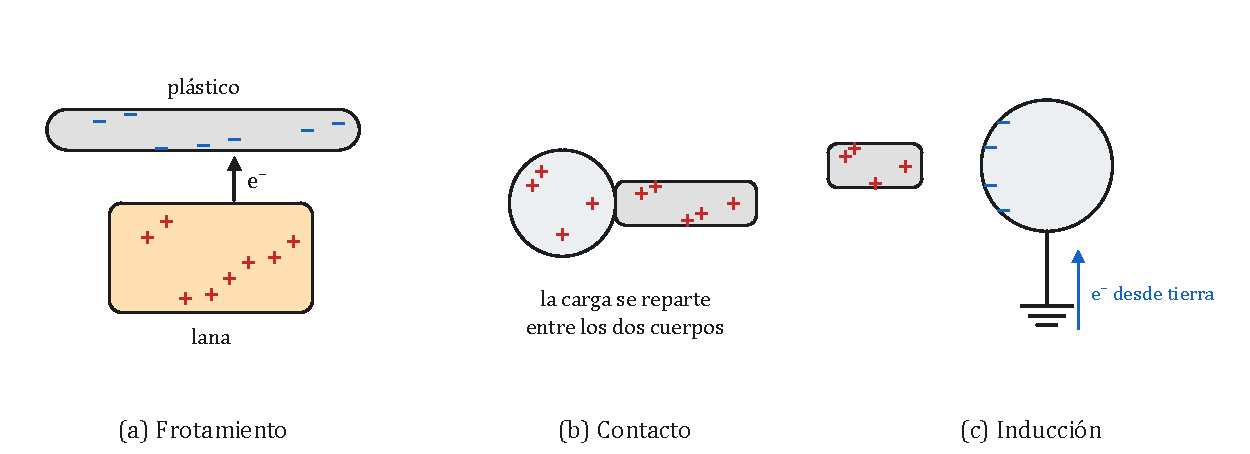
\includegraphics[width=0.8\textwidth]{images/UD11/electrizacion}
    \caption{Formas de electrizar un cuerpo: por frotamiento, por contacto y por inducción.}
    \label{fig:ud11-electrizacion}
\end{figure}

\begin{exercise}
    Un objeto de plástico frotado con un paño adquiere una carga de \qty{-3.2}{\nano\coulomb}. a) ¿Ha ganado o ha perdido electrones?
    ¿Cuántos? b) ¿Qué carga ha adquirido el paño?
    \begin{solu}
        a) \textcolor{red}{Ha ganado} \(\dfrac{\num{3.2e-9}}{\num{1.6e-19}} = \textcolor{red}{\num{2e10}~\text{electrones}}\).
        b) \textcolor{red}{\qty{+3.2}{\nano\coulomb}}: la carga se conserva, y el paño ha perdido esos electrones.
    \end{solu}
\end{exercise}

%========================================================================================
\section{Cómo se resuelve un problema de dinámica}\label{sec:ud11-esquema}
%========================================================================================

La segunda ley de Newton, \(\vec{F}_{\text{neta}} = m\,\vec{a}\), nos permite estudiar la evolución de un objeto en multitud de
situaciones. Para aplicarla bien hay que tener en cuenta dos cosas:

\begin{itemize}
    \item Es una ecuación \textbf{vectorial}, que equivale a una ecuación para cada componente:
    \(\sum F_x = m\,a_x\) y \(\sum F_y = m\,a_y\).
    \item Hay que \textbf{identificar bien todas las fuerzas} que actúan sobre el cuerpo: qué otro cuerpo las ejerce, en qué dirección
    actúan y cuánto valen.
\end{itemize}

\begin{definition}[Procedimiento para resolver un problema de dinámica]
    \textbf{1.}~\textbf{Representa el cuerpo} como un punto o una caja: no nos interesan su forma ni su tamaño, sino el movimiento de su
        centro de masas.

    \textbf{2.}~\textbf{Identifica y dibuja todas las fuerzas} que actúan sobre él (¿lo atrae otro cuerpo? ¿está apoyado? ¿hay rozamiento?
        ¿está unido a cuerdas o muelles?). Este dibujo se llama \textbf{diagrama de cuerpo libre}.

    \textbf{3.}~\textbf{Elige un sistema de referencia}, con un eje en la dirección del movimiento, y \textbf{descompón} las fuerzas que no
        estén sobre los ejes.

    \textbf{4.}~\textbf{Aplica la segunda ley de Newton} a cada eje y resuelve las ecuaciones.
\end{definition}

\begin{remark}
    Aunque se cumpla la tercera ley de Newton, en el diagrama solo se dibujan las fuerzas que actúan \textbf{sobre} el cuerpo que
    estudiamos, no las que él ejerce sobre otros. Si hay varios cuerpos, se dibuja un diagrama para cada uno y se plantean sus
    ecuaciones por separado.
\end{remark}

\begin{figure}[H]
    \centering
    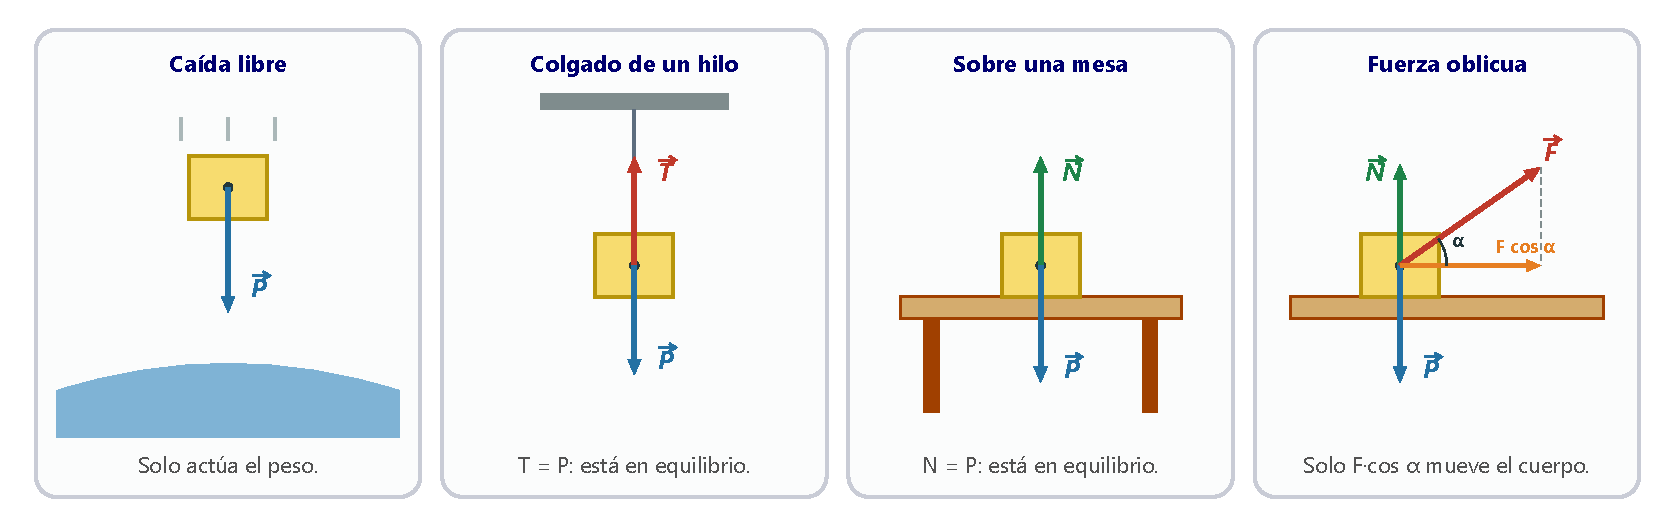
\includegraphics[width=\textwidth]{images/UD11/fuerzas_cuerpos}
    \caption{Diagramas de cuerpo libre de un cuerpo en algunas situaciones sencillas.}
    \label{fig:ud11-diagramas}
\end{figure}

%========================================================================================
\section{La interacción gravitatoria y el peso}\label{sec:ud11-gravitatoria}
%========================================================================================

\subsection{Ley de la gravitación universal}

Newton propuso en 1687, a partir de los trabajos de Kepler y de sus propias medidas, que todos los cuerpos se atraen por el simple
hecho de tener masa.

\begin{definition}[Ley de la gravitación universal]
    Dos cuerpos se atraen con una fuerza directamente proporcional al producto de sus masas e inversamente proporcional al cuadrado
    de la distancia que los separa:
    \[ F = G\,\frac{m_1\,m_2}{r^2} \qquad G = \qty{6.67e-11}{\newton\m\squared\per\kg\squared} \]
\end{definition}

\begin{itemize}
    \item La fuerza tiene la dirección de la recta que une los dos cuerpos y es siempre \textbf{atractiva}. Por la tercera ley de
    Newton, cada cuerpo atrae al otro con una fuerza del mismo módulo (figura~\ref{fig:ud11-gravitacion}).
    \item La \textbf{constante de gravitación universal}, \(G\), tiene el mismo valor en todo el universo. Es tan pequeña que solo los
    cuerpos de masa enorme, como los planetas, ejercen fuerzas gravitatorias apreciables.
\end{itemize}

\begin{figure}[H]
    \centering
    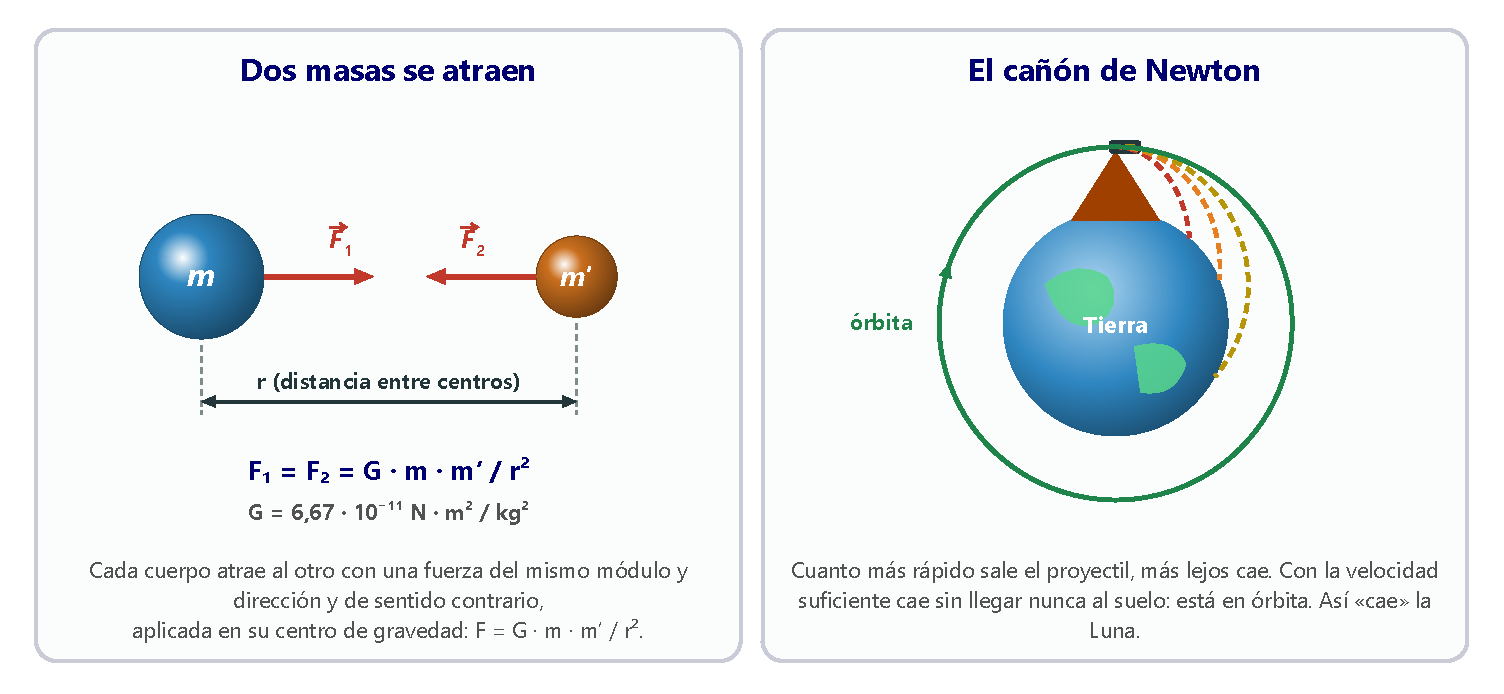
\includegraphics[width=0.55\textwidth]{images/UD11/gravitacion}
    \caption{Dos masas se atraen con fuerzas iguales y opuestas.}
    \label{fig:ud11-gravitacion}
\end{figure}

\subsection{El peso de los cuerpos}

El peso es un caso particular de la ley de la gravitación universal: es la fuerza con que la Tierra, de masa \(M_T\) y radio \(R_T\),
atrae a los cuerpos situados en su superficie:
\[ P = G\,\frac{M_T\,m}{R_T^2} = m\,g \qquad \text{con} \qquad g = G\,\frac{M_T}{R_T^2} = \qty{9.8}{\m\per\s\squared} \]

\begin{itemize}
    \item \textbf{Módulo}: \(P = m\,g\). \textbf{Dirección}: radial, la de la recta que une el cuerpo con el centro de la Tierra.
    \textbf{Sentido}: hacia el centro de la Tierra. \textbf{Punto de aplicación}: el centro de gravedad del cuerpo.
    \item El peso depende de la distancia al centro de la Tierra. La expresión \(P = m\,g\) con \(g = \qty{9.8}{\m\per\s\squared}\) solo
    vale cerca de la superficie, cuando la altura es pequeña comparada con el radio terrestre.
    \item En otros astros, \(g\) es distinta porque depende de su masa y de su radio. La masa de un astronauta es la misma en la Tierra
    y en la Luna, pero en la Luna, donde \(g = \qty{1.62}{\m\per\s\squared}\), pesa unas seis veces menos.
\end{itemize}

\begin{example}
    \textbf{El peso en la Estación Espacial.} ¿Cuánto pesa una astronauta de \qty{70}{\kg} en la Estación Espacial Internacional, a
    \qty{408}{\km} de altura? Compáralo con su peso en la superficie. (\(M_T = \qty{5.97e24}{\kg}\), \(R_T = \qty{6370}{\km}\).)

    \textbf{Solución.} La distancia al centro de la Tierra es \(r = 6370 + 408 = \qty{6778}{\km}\):
    \[ P = G\,\frac{M_T\,m}{r^2} = \num{6.67e-11} \cdot \frac{\num{5.97e24} \cdot 70}{(\num{6.778e6})^2} = \qty{607}{\newton} \]
    En la superficie pesaría \(70 \cdot \num{9.8} = \qty{686}{\newton}\): en la Estación pesa \textbf{un 88\,\%} de su peso habitual. Si
    los astronautas flotan no es porque no pesen, sino porque la Estación y todo lo que hay dentro caen juntos alrededor de la Tierra.
\end{example}

\begin{exercise}
    Calcula el peso de una persona de \qty{80}{\kg} en la Tierra, en la Luna, en Marte y en Venus. (\(g_L = \qty{1.62}{\m\per\s\squared}\);
    \(g_M = \qty{3.71}{\m\per\s\squared}\); \(g_V = \qty{8.87}{\m\per\s\squared}\).)
    \begin{solu}
        \textcolor{red}{Tierra: \qty{784}{\newton}; Luna: \qty{130}{\newton}; Marte: \qty{297}{\newton}; Venus: \qty{710}{\newton}.}
    \end{solu}
\end{exercise}

\begin{exercise}
    Una persona pesa \qty{130}{\newton} en la Luna. ¿Cuál es su masa? ¿Cuánto pesará en la Tierra?
    \begin{solu}
        \(m = \dfrac{130}{\num{1.62}} = \textcolor{red}{\qty{80.2}{\kg}}\); \(P_T = \num{80.2} \cdot \num{9.8} = \textcolor{red}{\qty{786}{\newton}}\).
    \end{solu}
\end{exercise}

%========================================================================================
\section{La interacción electrostática}\label{sec:ud11-electrostatica}
%========================================================================================

Frota un bolígrafo de plástico con un jersey de lana y acércalo a unos trocitos de papel: los atrae. Ya hacia el año 600 a.\,C., Tales
de Mileto observó que el ámbar frotado atraía objetos ligeros; de ahí viene la palabra \textit{electricidad}, del griego
\textit{elektron}, «ámbar». Las fuerzas entre cargas en reposo se llaman \textbf{electrostáticas}.

\begin{definition}[Ley de Coulomb]
    La fuerza entre dos cargas puntuales es directamente proporcional al producto de las cargas e inversamente proporcional al
    cuadrado de la distancia que las separa:
    \[ F = k\,\frac{|q_1\,q_2|}{r^2} \]
    En el vacío, \(k = \qty{9e9}{\newton\m\squared\per\coulomb\squared}\).
\end{definition}

Charles-Augustin de Coulomb la estableció en 1785 midiendo fuerzas con una balanza de torsión. Sus características son:
\begin{itemize}
    \item La fuerza tiene la dirección de la recta que une las cargas.
    \item A diferencia de la gravitatoria, puede ser \textbf{atractiva o repulsiva}: las cargas de distinto signo se atraen y las del
    mismo signo se repelen (figura~\ref{fig:ud11-coulomb}).
    \item La constante \(k\) depende del medio en que estén las cargas; en el agua, por ejemplo, es unas 80 veces menor que en el vacío.
    \item Las fuerzas electrostáticas también cumplen la tercera ley de Newton.
\end{itemize}

\begin{figure}[H]
    \centering
    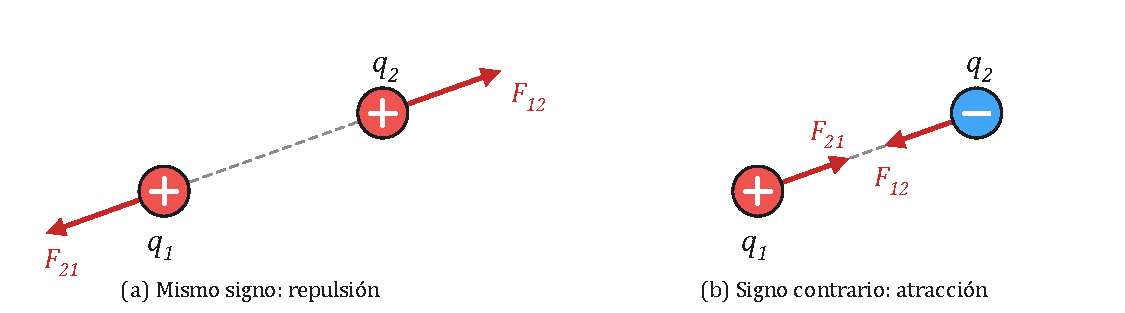
\includegraphics[width=0.75\textwidth]{images/UD11/coulomb}
    \caption{Fuerzas entre dos cargas: repulsión si tienen el mismo signo y atracción si tienen signos contrarios.}
    \label{fig:ud11-coulomb}
\end{figure}

\begin{example}
    \textbf{Fuerza eléctrica y fuerza gravitatoria entre dos iones.} En un cristal de sal común, un ion \ch{Na+} y un ion \ch{Cl-}
    están separados \qty{2.82e-10}{\m}. Calcula la fuerza electrostática y la gravitatoria entre ellos y compáralas. (Masas: \ch{Na}
    \qty{23}{\uma}, \ch{Cl} \qty{35.5}{\uma}; \(\qty{1}{\uma} = \qty{1.66e-27}{\kg}\).)

    \textbf{Solución.} Cada ion tiene una carga elemental, \(\num{1.6e-19}\)~C:
    \[ F_e = k\,\frac{|q_1\,q_2|}{r^2} = \num{9e9} \cdot \frac{(\num{1.6e-19})^2}{(\num{2.82e-10})^2} = \qty{2.9e-9}{\newton} \]
    \[ F_g = G\,\frac{m_1\,m_2}{r^2} = \num{6.67e-11} \cdot \frac{(23 \cdot \num{1.66e-27}) \cdot (\num{35.5} \cdot \num{1.66e-27})}{(\num{2.82e-10})^2}
    = \qty{1.9e-42}{\newton} \]
    La fuerza eléctrica es unas \(\num{1.5e33}\) veces mayor: en el mundo de los átomos la gravedad es completamente despreciable, y
    los enlaces químicos son de naturaleza eléctrica.
\end{example}

\begin{exercise}
    Calcula la fuerza con que se repelen dos bolitas con una carga de \qty{+3}{\micro\coulomb} cada una si están separadas
    \qty{15}{\cm}. Representa la fuerza sobre cada carga.
    \begin{solu}
        \(F = \num{9e9} \cdot \dfrac{(\num{3e-6})^2}{\num{0.15}^2} = \textcolor{red}{\qty{3.6}{\newton}}\), en la recta que las une y
        \textcolor{red}{alejando cada carga de la otra}.
    \end{solu}
\end{exercise}

\begin{exercise}
    ¿A qué distancia deben estar dos cargas de \qty{+20}{\nano\coulomb} y \qty{-20}{\nano\coulomb} para atraerse con una fuerza de
    \qty{0.3}{\newton}?
    \begin{solu}
        \(r = \sqrt{\dfrac{\num{9e9} \cdot (\num{2e-8})^2}{\num{0.3}}} = \textcolor{red}{\qty{3.5e-3}{\m}}\) (\qty{3.5}{\mm}).
    \end{solu}
\end{exercise}

%========================================================================================
\section{Fuerzas de contacto}\label{sec:ud11-contacto}
%========================================================================================

Las fuerzas de contacto solo actúan mientras los cuerpos se tocan: cuando cesa el contacto, cesa la interacción. Por eso, una vez
lanzada una pelota, la fuerza de la mano ya no actúa sobre ella. Aunque parezcan muy distintas, todas estas fuerzas se deben, a escala
microscópica, a interacciones electromagnéticas entre los átomos de las superficies.

\subsection{La fuerza normal}

Un libro apoyado en la mesa no la atraviesa ni cae, aunque la Tierra lo atrae. Si está en equilibrio, alguna fuerza compensa su peso:
la que le hace la mesa.

\begin{definition}[Fuerza normal]
    Es la fuerza que ejerce una superficie sobre un cuerpo apoyado en ella. Es la reacción de la superficie a la fuerza con que el
    cuerpo la presiona.
\end{definition}

\begin{itemize}
    \item Es siempre \textbf{perpendicular a la superficie de apoyo} y dirigida hacia fuera de ella.
    \item Su módulo \textbf{depende de las demás fuerzas} que actúan sobre el cuerpo: se obtiene aplicando la segunda ley en la
    dirección perpendicular a la superficie. No siempre es igual al peso.
    \item La normal \textbf{no es la reacción del peso}: el peso es una interacción Tierra-cuerpo y la normal, una interacción
    superficie-cuerpo.
    \item Solo hay normal si hay apoyo: si un cuerpo toca una superficie pero no la presiona, la normal es nula.
\end{itemize}

\begin{example}
    \textbf{Presionar un libro.} Empujamos hacia abajo con una fuerza de \qty{12}{\newton} un libro de \qty{1.5}{\kg} apoyado en una
    mesa. ¿Cuánto vale la normal?

    \textbf{Solución.} Sobre el libro actúan su peso y nuestra fuerza (hacia abajo) y la normal (hacia arriba). Está en equilibrio:
    \[ N - P - F = 0 \Rightarrow N = \num{1.5} \cdot \num{9.8} + 12 = \qty{26.7}{\newton} \]
\end{example}

\begin{exercise}
    Un bloque de \qty{3}{\kg} está sobre un plano inclinado \(25^\circ\). ¿Cuánto vale la fuerza normal?
    \begin{solu}
        \(N = P_y = 3 \cdot \num{9.8} \cdot \cos 25^\circ = \textcolor{red}{\qty{26.6}{\newton}}\).
    \end{solu}
\end{exercise}

\subsection{Fuerzas de rozamiento}

El rozamiento se debe a las \textbf{irregularidades} de las superficies, que encajan unas con otras, y a las fuerzas de adhesión entre
sus átomos. Siempre se \textbf{opone al movimiento relativo} de un cuerpo respecto a otro.

\begin{definition}[Fuerza de rozamiento]
    Es una fuerza paralela a la superficie de contacto entre dos cuerpos que se opone al deslizamiento de uno respecto al otro.
\end{definition}

\paragraph{Rozamiento estático.} Si intentamos arrastrar un mueble pesado empujando poco a poco con más fuerza, al principio no se
mueve: el rozamiento \textbf{estático} iguala a la fuerza aplicada. Su valor no es fijo: crece con la fuerza aplicada hasta un
\textbf{valor máximo}
\[ F_{re,\,\text{máx}} = \mu_e\,N \]
donde \(\mu_e\) es el \textbf{coeficiente de rozamiento estático}. Solo cuando la fuerza aplicada supera ese máximo el cuerpo empieza
a moverse.

\paragraph{Rozamiento cinético.} Una vez en movimiento, sobre el cuerpo actúa el rozamiento \textbf{cinético} (o dinámico):
\[ F_{rc} = \mu_c\,N \]
donde \(\mu_c\) es el \textbf{coeficiente de rozamiento cinético}. Consideraremos que su valor es constante y no depende de la velocidad.

\begin{figure}[H]
    \centering
    \begin{tikzpicture}
        \begin{axis}[grafica, width=0.55\linewidth, height=5cm, xlabel={Fuerza aplicada, \(F\)}, ylabel={\(F_r\)}, xmin=0, xmax=10,
            ymin=0, ymax=6, xtick={5}, xticklabels={\(\mu_e N\)}, ytick={3.6,5}, yticklabels={\(\mu_c N\),\(\mu_e N\)}]
            \addplot[very thick, ocre, domain=0:5] {x};
            \addplot[very thick, ocre, domain=5:10] {3.6};
            \addplot[dashed, gray] coordinates {(5,5) (5,3.6)};
            \node[font=\scriptsize, align=center] at (axis cs:2.4,4.4) {estático:\\ \(F_r = F\)};
            \node[font=\scriptsize] at (axis cs:7.6,4.2) {cinético};
            \node[font=\scriptsize] at (axis cs:7.6,1.6) {el cuerpo se mueve};
        \end{axis}
    \end{tikzpicture}
    \caption{Fuerza de rozamiento frente a la fuerza aplicada. En reposo, el rozamiento iguala a la fuerza aplicada hasta su valor
    máximo; una vez en movimiento, vale \(\mu_c\,N\), algo menos.}
    \label{fig:ud11-rozamiento}
\end{figure}

\begin{itemize}
    \item Los coeficientes \(\mu_e\) y \(\mu_c\) no tienen unidades y dependen de \textbf{las dos superficies} en contacto
    (tabla~\ref{tab:ud11-coeficientes}), pero apenas dependen del área de contacto.
    \item Normalmente \(\mu_e > \mu_c\): cuesta más poner un cuerpo en movimiento que mantenerlo.
\end{itemize}

\begin{table}[H]
    \centering
    \caption{Valores aproximados de los coeficientes de rozamiento}
    \vspace{-5pt}
    \begin{tabular}{@{}lcc@{}}
        \toprule
        \textbf{Superficies} & \(\boldsymbol{\mu_e}\) & \(\boldsymbol{\mu_c}\) \\
        \midrule
        Madera sobre madera & \num{0.25}-\num{0.5} & \num{0.2} \\[3pt]
        Madera sobre cuero & \num{0.5} & \num{0.4} \\[3pt]
        Acero sobre acero & \num{0.74} & \num{0.57} \\[3pt]
        Neumático sobre asfalto seco & \num{1.0} & \num{0.8} \\[3pt]
        Neumático sobre asfalto mojado & \num{0.7} & \num{0.5} \\[3pt]
        Acero sobre hielo & \num{0.03} & \num{0.01} \\
        \bottomrule
    \end{tabular}
    \label{tab:ud11-coeficientes}
\end{table}

\begin{remark}
    A veces interesa reducir el rozamiento (puliendo las superficies o usando lubricantes, como el aceite de un motor o el líquido
    sinovial de nuestras articulaciones) y otras, aumentarlo (los dibujos de los neumáticos o las suelas de las zapatillas). Sin
    rozamiento no podríamos ni caminar.
\end{remark}

\begin{example}
    \textbf{Arrastrar un cuerpo.} Un cuerpo de \qty{50}{\kg} está en reposo en el suelo. Los coeficientes de rozamiento son
    \(\mu_e = \num{0.45}\) y \(\mu_c = \num{0.30}\). Calcula: a) la fuerza horizontal mínima para ponerlo en movimiento; b) la fuerza de
    rozamiento y la aceleración si se empuja con \qty{300}{\newton}.

    \textbf{Solución.} La normal es igual al peso: \(N = 50 \cdot \num{9.8} = \qty{490}{\newton}\).
    a) \(F_{re,\,\text{máx}} = \mu_e\,N = \num{0.45} \cdot 490 = \qty{220.5}{\newton}\): hay que empujar con algo más de esa fuerza.
    b) Como \(300 > \num{220.5}\), el cuerpo se mueve y el rozamiento es cinético: \(F_r = \num{0.30} \cdot 490 = \qty{147}{\newton}\);
    \(a = \dfrac{300 - 147}{50} = \qty{3.06}{\m\per\s\squared}\).
\end{example}

\begin{exercise}
    Se aprieta un cuerpo de \qty{3}{\kg} contra una pared vertical con una fuerza horizontal de \qty{70}{\newton}. El coeficiente de
    rozamiento estático es \num{0.5}. a) ¿Resbalará? b) ¿Qué fuerza de rozamiento actúa? ¿Qué fuerza hace la pared?
    \begin{solu}
        \textcolor{blue}{\(N = \qty{70}{\newton}\); \(F_{re,\,\text{máx}} = \num{0.5} \cdot 70 = \qty{35}{\newton}\) y \(P = \qty{29.4}{\newton}\).}
        a) \textcolor{red}{No resbala}, porque \(P\) es menor que el rozamiento máximo. b) \(\textcolor{red}{F_r = \qty{29.4}{\newton}}\)
        hacia arriba; la pared hace una normal de \textcolor{red}{\qty{70}{\newton}} (y además el rozamiento).
    \end{solu}
\end{exercise}

\begin{exercise}
    Para mover una lavadora de \qty{50}{\kg} por el suelo de la cocina hay que empujarla con \qty{240}{\newton} antes de que empiece
    a deslizar. a) Calcula el coeficiente de rozamiento estático. b) Si con esa misma fuerza la lavadora adquiere una aceleración de
    \qty{1}{\m\per\s\squared}, ¿cuál es el coeficiente cinético?
    \begin{solu}
        a) \(\mu_e = \dfrac{240}{490} = \textcolor{red}{\num{0.49}}\). b) \(F_r = 240 - 50 \cdot 1 = \qty{190}{\newton}\);
        \(\mu_c = \dfrac{190}{490} = \textcolor{red}{\num{0.39}}\).
    \end{solu}
\end{exercise}

\subsection{La tensión}

\begin{definition}[Tensión]
    Es la fuerza que transmite una cuerda o un cable tenso a los cuerpos unidos a sus extremos.
\end{definition}

\begin{itemize}
    \item Tiene la \textbf{dirección de la cuerda} y su sentido va desde el cuerpo hacia la cuerda: una cuerda solo puede tirar, nunca
    empujar.
    \item Su valor se calcula con la segunda ley de Newton, teniendo en cuenta las demás fuerzas que actúan sobre el cuerpo.
\end{itemize}

Supondremos que las cuerdas son \textbf{inextensibles} (no cambian de longitud) y de \textbf{masa despreciable}; entonces la tensión
vale lo mismo en todos los puntos de una cuerda. Si la tensión supera un \textbf{valor máximo}, que depende del material, la cuerda se
rompe. En la sogatira, la fuerza con que tira cada participante se transmite por la cuerda a los del otro equipo.

\begin{example}
    \textbf{Una grúa.} Una grúa levanta una carga de \qty{1000}{\kg} con una aceleración de \qty{2}{\m\per\s\squared}. El cable
    resiste una tensión máxima de \qty{14000}{\newton}. a) Dibuja las fuerzas y calcula la tensión. b) ¿Podría subir a velocidad
    constante una carga de \qty{1500}{\kg}?

    \textbf{Solución.} a) Sobre la carga actúan la tensión (hacia arriba) y el peso (hacia abajo):
    \[ T - m\,g = m\,a \Rightarrow T = m\,(g + a) = 1000 \cdot (\num{9.8} + 2) = \qty{11800}{\newton} \]
    b) A velocidad constante, \(T = m\,g = 1500 \cdot \num{9.8} = \qty{14700}{\newton}\), más de lo que resiste el cable: \textbf{se
    rompería}. La carga máxima a velocidad constante es \(\dfrac{14000}{\num{9.8}} = \qty{1429}{\kg}\).
\end{example}

\begin{exercise}
    El ascensor de un hospital, de \qty{800}{\kg}, sube a un grupo de personas que suman \qty{450}{\kg} con una aceleración de
    \qty{1.2}{\m\per\s\squared}. a) Dibuja las fuerzas que actúan sobre el ascensor. b) Calcula la tensión del cable. c) ¿Qué fuerza
    hace el suelo del ascensor sobre las personas?
    \begin{solu}
        b) \(T = 1250 \cdot (\num{9.8} + \num{1.2}) = \textcolor{red}{\qty{13750}{\newton}}\).
        c) \(N = 450 \cdot 11 = \textcolor{red}{\qty{4950}{\newton}}\) (más que su peso, \qty{4410}{\newton}).
    \end{solu}
\end{exercise}

\subsection{Fuerzas elásticas: ley de Hooke}

Las fuerzas pueden cambiar el movimiento de un cuerpo y también deformarlo. Cuando estiramos o comprimimos un muelle o una goma, el
material ejerce una fuerza que tiende a devolverlo a su forma: la \textbf{fuerza elástica} o \textbf{recuperadora}.

\begin{definition}[Ley de Hooke]
    La fuerza elástica que ejerce un muelle es proporcional a su deformación y se opone a ella:
    \[ F_{\text{elástica}} = -k\,\Delta L \]
    \begin{itemize}
        \item \(k\) es la \textbf{constante elástica} del muelle, en \unit{\newton\per\m}. Cuanto mayor es, más rígido es el muelle.
        \item \(\Delta L = L - L_0\) es la deformación: positiva si el muelle se estira y negativa si se comprime.
        \item El signo negativo indica que la fuerza tiene sentido contrario a la deformación.
    \end{itemize}
\end{definition}

La fuerza recuperadora es la reacción del muelle a la fuerza que lo deforma (tercera ley de Newton). La ley de Hooke solo es válida
para deformaciones pequeñas: si se sobrepasa el \textbf{límite de elasticidad}, el material queda deformado permanentemente o se
rompe. Nuestros tendones también se comportan como materiales elásticos, y superar su límite causa lesiones.

\begin{example}
    \textbf{Un muelle.} Un muelle se estira \qty{12}{\cm} al colgarle un cuerpo de \qty{15}{\kg}. a) ¿Cuál es su constante elástica?
    b) ¿Cuánto se estirará con un cuerpo de \qty{22}{\kg}?

    \textbf{Solución.} a) En equilibrio, la fuerza elástica iguala al peso: \(k\,\Delta L = m\,g \Rightarrow k = \dfrac{15 \cdot \num{9.8}}{\num{0.12}}
    = \qty{1225}{\newton\per\m}\). b) \(\Delta L = \dfrac{22 \cdot \num{9.8}}{1225} = \qty{0.176}{\m} = \qty{17.6}{\cm}\).
\end{example}

\begin{exercise}
    Un muelle de \qty{30}{\cm} pasa a medir \qty{36}{\cm} cuando tiramos de él con una fuerza de \qty{4.2}{\newton}. a) Calcula su
    constante elástica. b) ¿Cuánto medirá si tiramos con \qty{6.3}{\newton}?
    \begin{solu}
        a) \(k = \dfrac{\num{4.2}}{\num{0.06}} = \textcolor{red}{\qty{70}{\newton\per\m}}\). b) \(\Delta L = \dfrac{\num{6.3}}{70} =
        \qty{0.09}{\m}\): \(L = \textcolor{red}{\qty{39}{\cm}}\).
    \end{solu}
\end{exercise}

%========================================================================================
\section{Dinámica del movimiento rectilíneo}\label{sec:ud11-rectilineo}
%========================================================================================

En un movimiento rectilíneo no hay aceleración normal, así que \textbf{no hay fuerza neta perpendicular a la velocidad}: la fuerza
resultante tiene la dirección del movimiento. Si tiene el mismo sentido que la velocidad, el cuerpo acelera; si tiene sentido
contrario, frena. Una vez conocida la aceleración, las ecuaciones de la cinemática nos dan la velocidad y la posición en cada instante.

\subsection{Planos horizontales}

Seguimos el procedimiento general. Conviene tomar el eje \(X\) en la dirección y el sentido del movimiento: así, las fuerzas a favor del
movimiento son positivas y las que se oponen, negativas. Si la fuerza aplicada es oblicua, su componente vertical cambia el valor de la
normal y, con ella, el del rozamiento:
\begin{itemize}
    \item Si tiramos \textbf{hacia arriba} formando un ángulo \(\alpha\): \(N = m\,g - F\sen\alpha\) (el rozamiento disminuye).
    \item Si empujamos \textbf{hacia abajo} formando un ángulo \(\alpha\): \(N = m\,g + F\sen\alpha\) (el rozamiento aumenta).
\end{itemize}

\begin{example}
    \textbf{Pintar las líneas de un campo.} Un operario empuja una carretilla de marcar campos de \qty{18}{\kg} con una fuerza de
    \qty{120}{\newton} dirigida hacia abajo formando \(35^\circ\) con la horizontal, y la carretilla avanza con velocidad constante.
    a) Dibuja las fuerzas. b) Calcula la fuerza de rozamiento y el coeficiente de rozamiento. c) ¿Con qué fuerza tendría que empujar
    para que, partiendo del reposo, alcanzara \qty{1.5}{\m\per\s} en \qty{2}{\s}?

    \textbf{Solución.} a) Actúan el peso, la normal, la fuerza del operario y el rozamiento.

    b) Velocidad constante, \(a = 0\). Eje \(X\): \(F_r = F\cos 35^\circ = \qty{98.3}{\newton}\). Eje \(Y\):
    \(N = m\,g + F\sen 35^\circ = \num{176.4} + \num{68.8} = \qty{245.2}{\newton}\). Por tanto, \(\mu = \dfrac{\num{98.3}}{\num{245.2}} = \num{0.40}\).

    c) Ahora \(a = \dfrac{\num{1.5}}{2} = \qty{0.75}{\m\per\s\squared}\), y al cambiar \(F\) cambian la normal y el rozamiento:
    \[ F\cos 35^\circ - \mu\,(m\,g + F\sen 35^\circ) = m\,a \Rightarrow F = \frac{m\,a + \mu\,m\,g}{\cos 35^\circ - \mu\sen 35^\circ}
    = \frac{\num{13.5} + \num{70.7}}{\num{0.589}} = \qty{143}{\newton} \]
\end{example}

\begin{example}
    \textbf{Empujar un paquete con el pie.} Una persona con las manos ocupadas empuja con el pie un paquete de \qty{12}{\kg} con una
    fuerza de \qty{70}{\newton} que forma \(40^\circ\) por debajo de la horizontal. Si \(\mu = \num{0.3}\), ¿qué aceleración tiene?

    \textbf{Solución.} \(F_x = 70\cos 40^\circ = \qty{53.6}{\newton}\); \(F_y = 70\sen 40^\circ = \qty{45.0}{\newton}\) hacia abajo.
    Eje \(Y\): \(N = \num{117.6} + \num{45.0} = \qty{162.6}{\newton}\); \(F_r = \num{0.3} \cdot \num{162.6} = \qty{48.8}{\newton}\).
    Eje \(X\): \(a = \dfrac{\num{53.6} - \num{48.8}}{12} = \qty{0.40}{\m\per\s\squared}\). Empujar hacia abajo es poco eficaz: buena
    parte de la fuerza solo aumenta el rozamiento.
\end{example}

\begin{exercise}
    Queremos mover un sofá de \qty{40}{\kg} por un suelo sin rozamiento aplicando una fuerza de \qty{150}{\newton}. Calcula la
    aceleración si la fuerza: a) es horizontal; b) forma \(25^\circ\) por encima de la horizontal; c) forma \(25^\circ\) por debajo.
    \begin{solu}
        a) \(a = \textcolor{red}{\qty{3.75}{\m\per\s\squared}}\). b) y c) \(a = \dfrac{150\cos 25^\circ}{40} = \textcolor{red}{\qty{3.40}{\m\per\s\squared}}\)
        en ambos casos: sin rozamiento, la componente vertical no influye en el movimiento.
    \end{solu}
\end{exercise}

\begin{exercise}
    Dos niños empujan horizontalmente un carro de supermercado de \qty{8}{\kg} con una fuerza de \qty{35}{\newton}. Si \(\mu = \num{0.3}\),
    calcula la fuerza de rozamiento, la aceleración y la velocidad del carro después de recorrer \qty{12}{\m} partiendo del reposo.
    \begin{solu}
        \(F_r = \num{0.3} \cdot 8 \cdot \num{9.8} = \textcolor{red}{\qty{23.5}{\newton}}\); \(a = \dfrac{35 - \num{23.5}}{8} =
        \textcolor{red}{\qty{1.44}{\m\per\s\squared}}\); \(v = \sqrt{2 \cdot \num{1.44} \cdot 12} = \textcolor{red}{\qty{5.87}{\m\per\s}}\).
    \end{solu}
\end{exercise}

\begin{exercise}
    Para limpiar los cristales de una ventana apretamos contra ellos un trapo de \qty{150}{\g}. Si el coeficiente de rozamiento estático
    es \num{0.5}, ¿qué fuerza perpendicular al cristal hay que hacer, como mínimo, para que el trapo no caiga?
    \begin{solu}
        \(\mu_e\,F = m\,g \Rightarrow F = \dfrac{\num{0.15} \cdot \num{9.8}}{\num{0.5}} = \textcolor{red}{\qty{2.94}{\newton}}\).
    \end{solu}
\end{exercise}

\subsection{Planos inclinados}

Un \textbf{plano inclinado} es una superficie plana que forma un ángulo agudo con la horizontal. Es una de las máquinas simples más
antiguas: permite subir un cuerpo haciendo menos fuerza que si lo levantáramos en vertical. Para resolver estos problemas:

\begin{enumerate}[label=\numberballgreen]
    \item Toma el eje \(X\) paralelo al plano y el eje \(Y\) perpendicular a él. El sentido positivo del eje \(X\) decide el signo de
    fuerzas, velocidades y aceleraciones.
    \item Siempre actúan, al menos, el peso y la normal, que no tienen la misma dirección.
    \item Descompón el peso (figura~\ref{fig:ud11-plano}):
    \[ P_x = m\,g\sen\alpha \;\;\text{(paralela al plano)} \qquad P_y = m\,g\cos\alpha \;\;\text{(perpendicular al plano)} \]
    \item Si no hay otras fuerzas perpendiculares al plano, \(N = P_y = m\,g\cos\alpha\), porque el cuerpo no se mueve en esa
    dirección.
\end{enumerate}

\begin{figure}[H]
    \centering
    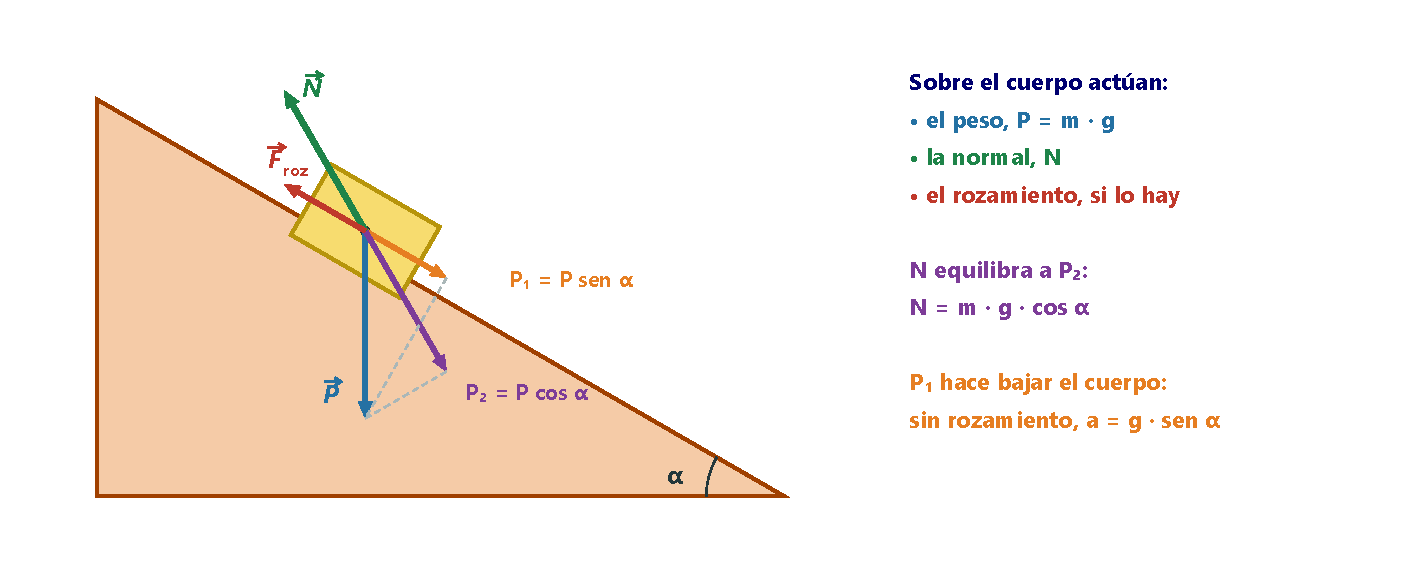
\includegraphics[width=0.8\textwidth]{images/UD10/plano_inclinado}
    \caption{Fuerzas sobre un cuerpo en un plano inclinado y componentes del peso (aquí \(P_1 = P_x\) y \(P_2 = P_y\)).}
    \label{fig:ud11-plano}
\end{figure}

\begin{example}
    \textbf{Un estuche por la mesa.} Una alumna inclina su mesa \(18^\circ\) y empuja hacia abajo, paralelamente a la mesa, su estuche
    de \qty{600}{\g} con una fuerza de \qty{4}{\newton}. Calcula la aceleración del estuche: a) sin rozamiento; b) con \(\mu = \num{0.25}\).

    \textbf{Solución.} Tomamos positivo el sentido hacia abajo del plano. \(P = \num{0.6} \cdot \num{9.8} = \qty{5.88}{\newton}\);
    \(P_x = \num{5.88}\sen 18^\circ = \qty{1.82}{\newton}\); \(P_y = N = \num{5.88}\cos 18^\circ = \qty{5.59}{\newton}\).

    a) \(F + P_x = m\,a \Rightarrow a = \dfrac{4 + \num{1.82}}{\num{0.6}} = \qty{9.70}{\m\per\s\squared}\).

    b) \(F_r = \num{0.25} \cdot \num{5.59} = \qty{1.40}{\newton}\); \(a = \dfrac{4 + \num{1.82} - \num{1.40}}{\num{0.6}} = \qty{7.36}{\m\per\s\squared}\).
\end{example}

\begin{example}
    \textbf{Lanzar hacia arriba por un tobogán.} La misma alumna lanza su estuche hacia arriba por un tobogán inclinado \(25^\circ\),
    con una velocidad de \qty{3}{\m\per\s}. Si \(\mu = \num{0.3}\), ¿qué distancia recorre hasta pararse?

    \textbf{Solución.} Ahora tomamos positivo el sentido del movimiento (hacia arriba). Tanto \(P_x\) como el rozamiento se oponen:
    \(P_x = \num{5.88}\sen 25^\circ = \qty{2.48}{\newton}\); \(N = \num{5.88}\cos 25^\circ = \qty{5.33}{\newton}\); \(F_r = \qty{1.60}{\newton}\).
    \[ -P_x - F_r = m\,a \Rightarrow a = -\frac{\num{2.48} + \num{1.60}}{\num{0.6}} = \qty{-6.81}{\m\per\s\squared} \]
    Con la cinemática: \(v^2 = v_0^2 + 2\,a\,\Delta x \Rightarrow \Delta x = \dfrac{0 - 3^2}{2 \cdot (\num{-6.81})} = \qty{0.66}{\m}\).
\end{example}

\begin{exercise}
    Un camión empieza a verter la leña que transporta cuando la inclinación del volquete llega a \(28^\circ\). ¿Cuál es el
    coeficiente de rozamiento estático entre la leña y el volquete?
    \begin{solu}
        \textcolor{blue}{Justo antes de deslizar, \(m\,g\sen\alpha = \mu_e\,m\,g\cos\alpha\).} \(\mu_e = \tg 28^\circ = \textcolor{red}{\num{0.53}}\).
    \end{solu}
\end{exercise}

\begin{exercise}
    Un bloque de \qty{3}{\kg} está en un plano inclinado \(30^\circ\) y se empuja hacia abajo con una fuerza de \qty{10}{\newton}
    paralela al plano. Calcula su aceleración: a) sin rozamiento; b) con \(\mu = \num{0.25}\).
    \begin{solu}
        \(P_x = \qty{14.7}{\newton}\), \(N = \qty{25.5}{\newton}\). a) \(a = \dfrac{10 + \num{14.7}}{3} = \textcolor{red}{\qty{8.23}{\m\per\s\squared}}\).
        b) \(F_r = \qty{6.37}{\newton}\): \(a = \dfrac{\num{24.7} - \num{6.37}}{3} = \textcolor{red}{\qty{6.11}{\m\per\s\squared}}\).
    \end{solu}
\end{exercise}

\subsection{Cuerpos enlazados}

Muchas veces varios cuerpos se mueven juntos unidos por cuerdas: una grúa que arrastra un coche, los vagones de un tren, una polea con
dos pesas (figura~\ref{fig:ud11-enlazados}). Para resolver estos problemas:

\begin{enumerate}[label=\numberballgreen]
    \item Si las cuerdas son inextensibles y sin masa, la distancia entre los cuerpos no cambia: todos tienen la misma velocidad y la
    misma aceleración en \textbf{módulo}, y la tensión es la misma en toda la cuerda.
    \item Elige un sistema de referencia para cada cuerpo, con el eje \(X\) en la dirección de su movimiento.
    \item Aplica la segunda ley a \textbf{cada cuerpo por separado}, con solo las fuerzas que actúan sobre él. Obtendrás un sistema de
    ecuaciones cuyas incógnitas suelen ser la aceleración y la tensión.
\end{enumerate}

\begin{figure}[H]
    \centering
    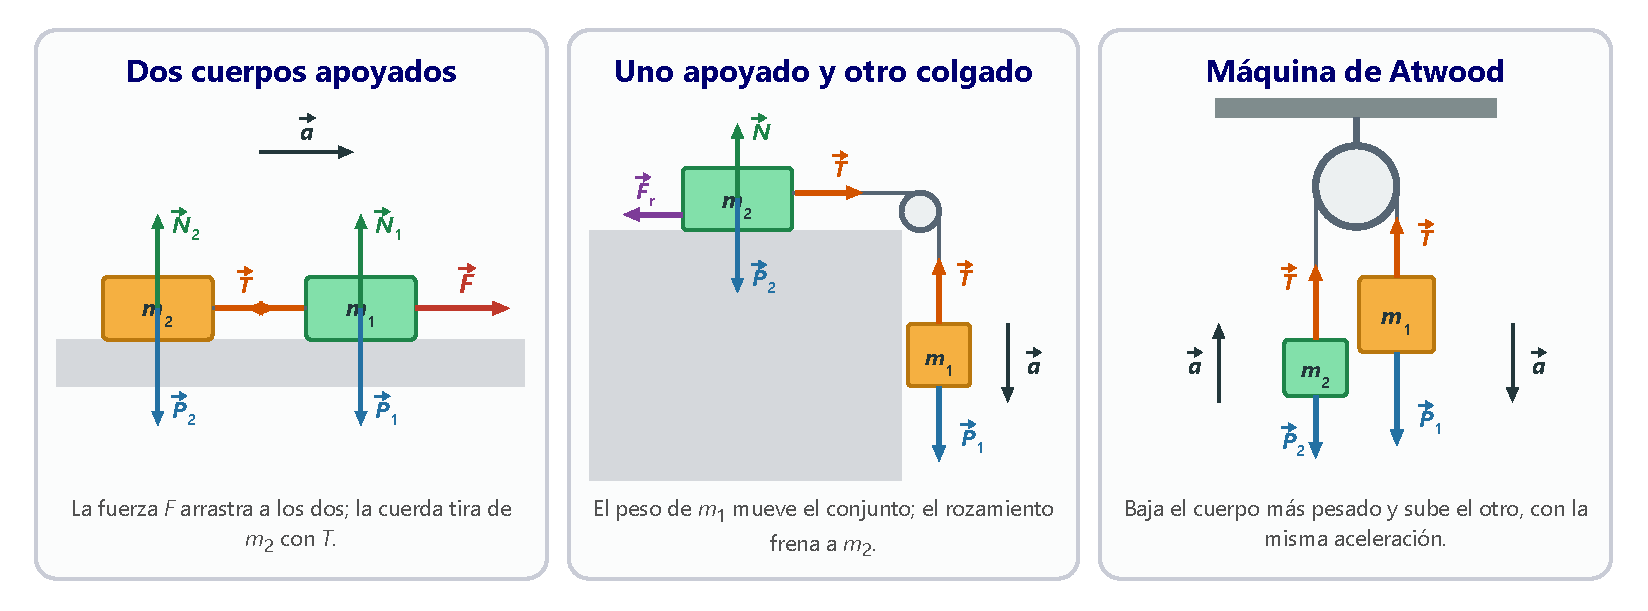
\includegraphics[width=\textwidth]{images/UD11/cuerpos_enlazados}
    \caption{Fuerzas sobre cuerpos enlazados en tres situaciones típicas.}
    \label{fig:ud11-enlazados}
\end{figure}

\begin{remark}
    Si solo queremos la aceleración, podemos tratar el conjunto como un solo cuerpo de masa \(m_1 + m_2\): las tensiones son fuerzas
    interiores y se cancelan. Para calcular la tensión, en cambio, hay que aplicar la segunda ley a uno de los cuerpos.
\end{remark}

\begin{example}
    \textbf{Dos bloques arrastrados.} Dos bloques de \(m_1 = \qty{20}{\kg}\) y \(m_2 = \qty{30}{\kg}\), unidos por una cuerda, se
    arrastran por el suelo sin rozamiento tirando de \(m_1\) con una fuerza horizontal de \qty{400}{\newton}
    (figura~\ref{fig:ud11-enlazados}, izquierda). Calcula la aceleración y la tensión de la cuerda.

    \textbf{Solución.} Sobre el conjunto, la única fuerza horizontal exterior es \(F\):
    \(a = \dfrac{F}{m_1 + m_2} = \dfrac{400}{50} = \qty{8}{\m\per\s\squared}\).
    Sobre \(m_2\) solo tira la cuerda: \(T = m_2\,a = 30 \cdot 8 = \qty{240}{\newton}\). (Comprobación con \(m_1\):
    \(F - T = 400 - 240 = 160 = 20 \cdot 8\).)
\end{example}

\begin{example}
    \textbf{Un bloque en la mesa y otro colgado.} Un cuerpo de \(m_1 = \qty{8}{\kg}\) cuelga de una cuerda que pasa por una polea y
    está unida a otro de \(m_2 = \qty{5}{\kg}\) apoyado en una mesa (figura~\ref{fig:ud11-enlazados}, centro). Si el coeficiente de
    rozamiento entre \(m_2\) y la mesa es \num{0.2}, calcula la aceleración y la tensión.

    \textbf{Solución.} El conjunto se mueve en el sentido en que cae \(m_1\). Ecuaciones de cada cuerpo:
    \[ m_2:\; T - \mu\,m_2\,g = m_2\,a \qquad\qquad m_1:\; m_1\,g - T = m_1\,a \]
    Sumándolas se elimina la tensión:
    \[ a = g\,\frac{m_1 - \mu\,m_2}{m_1 + m_2} = \num{9.8} \cdot \frac{8 - \num{0.2} \cdot 5}{13} = \qty{5.28}{\m\per\s\squared} \]
    Con la ecuación de \(m_1\): \(T = m_1\,(g - a) = 8 \cdot (\num{9.8} - \num{5.28}) = \qty{36.2}{\newton}\).
\end{example}

\paragraph{La máquina de Atwood.} Es una polea con una cuerda de cuyos extremos cuelgan dos cuerpos de masas parecidas
(figura~\ref{fig:ud11-enlazados}, derecha). La inventó George Atwood en 1784 para comprobar las leyes de la dinámica. Si \(m_1 > m_2\),
\(m_1\) baja y \(m_2\) sube con la misma aceleración:
\[ m_1\,g - T = m_1\,a \qquad T - m_2\,g = m_2\,a \qquad\Longrightarrow\qquad a = \frac{m_1 - m_2}{m_1 + m_2}\,g \]
Como la aceleración es mucho menor que \(g\), el movimiento es lento y fácil de medir: es una forma sencilla de medir \(g\).

\begin{exercise}
    Calcula la aceleración y la tensión del ejemplo de los dos bloques arrastrados si el coeficiente de rozamiento con el suelo es
    \num{0.1}.
    \begin{solu}
        \(a = \dfrac{400 - \num{0.1} \cdot 50 \cdot \num{9.8}}{50} = \textcolor{red}{\qty{7.02}{\m\per\s\squared}}\);
        \(T = 30 \cdot \num{7.02} + \num{0.1} \cdot 30 \cdot \num{9.8} = \textcolor{red}{\qty{240}{\newton}}\) (no cambia).
    \end{solu}
\end{exercise}

\begin{exercise}
    En una máquina de Atwood cuelgan dos cuerpos de \qty{6}{\kg} y \qty{9}{\kg}. Determina el sentido del movimiento, la aceleración y
    la tensión de la cuerda.
    \begin{solu}
        \textcolor{red}{Baja el de \qty{9}{\kg}}. \(a = \dfrac{3}{15} \cdot \num{9.8} = \textcolor{red}{\qty{1.96}{\m\per\s\squared}}\);
        \(T = 6 \cdot (\num{9.8} + \num{1.96}) = \textcolor{red}{\qty{70.6}{\newton}}\).
    \end{solu}
\end{exercise}

%========================================================================================
\section{Dinámica del movimiento circular}\label{sec:ud11-circular}
%========================================================================================

El movimiento circular está por todas partes: los satélites que orbitan la Tierra, los huracanes, una atracción de feria o la ropa
en el tambor de una lavadora. En un movimiento circular, la dirección de la velocidad cambia continuamente, así que hay una
\textbf{aceleración normal o centrípeta}, \(\vec{a}_n\), dirigida hacia el centro. Por la segunda ley, tiene que haber una fuerza que
la produzca.

\begin{definition}[Fuerza centrípeta]
    Es la resultante de todas las fuerzas que actúan sobre un cuerpo en la dirección perpendicular a su velocidad. Tiene dirección
    radial, sentido hacia el centro de la circunferencia y módulo
    \[ F_c = m\,a_c = m\,\frac{v^2}{r} = m\,\omega^2\,r \]
\end{definition}

\begin{remark}
    La fuerza centrípeta \textbf{no es una fuerza nueva}, sino el papel que hacen otras: el peso, la tensión de una cuerda, el
    rozamiento, la normal o una combinación de ellas. Si desaparece, el cuerpo sigue en línea recta, tangente a la trayectoria
    (figura~\ref{fig:ud11-centripeta}). La llamada «fuerza centrífuga» solo aparece al describir el movimiento desde un sistema de
    referencia que gira con el cuerpo, que no es inercial.
\end{remark}

\begin{figure}[H]
    \centering
    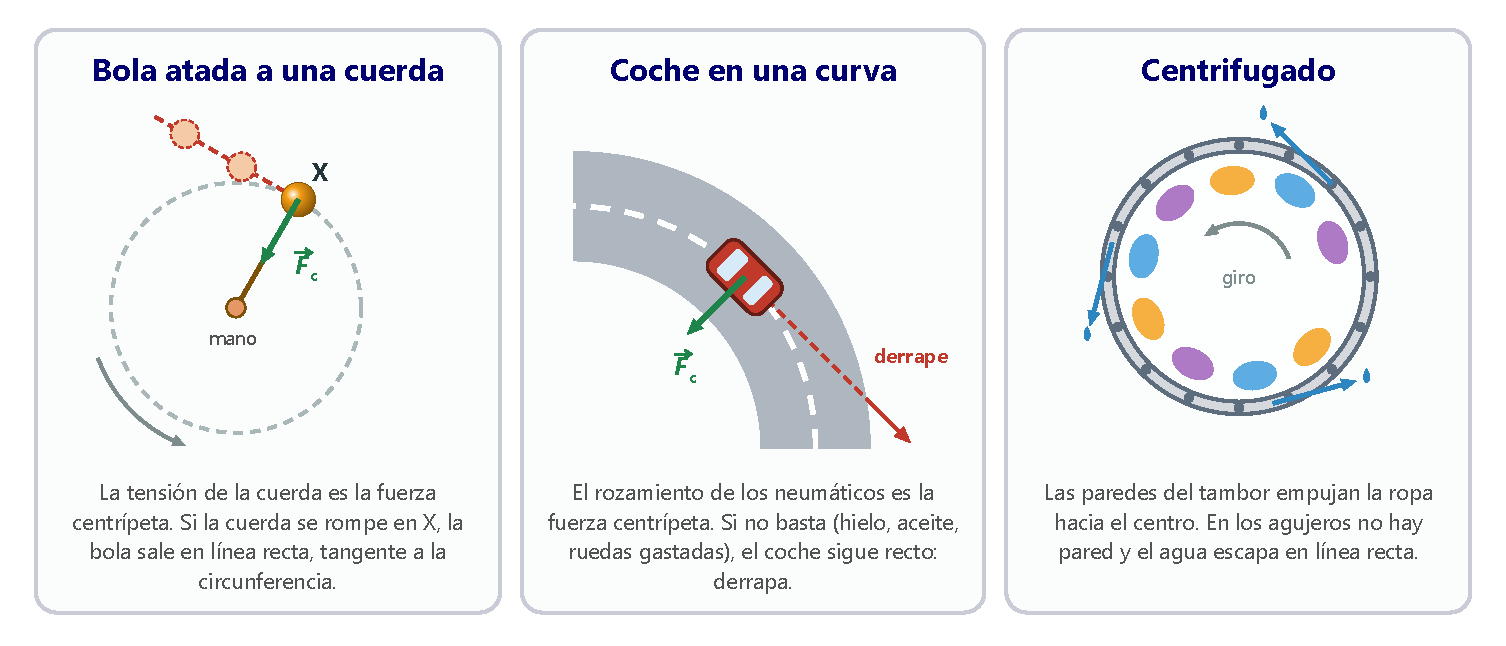
\includegraphics[width=\textwidth]{images/UD11/sin_fuerza_centripeta}
    \caption{Tres ejemplos de fuerza centrípeta y qué ocurre cuando falta.}
    \label{fig:ud11-centripeta}
\end{figure}

\paragraph{MCU y MCUA.} En un \textbf{MCU} el módulo de la velocidad no cambia: no hay aceleración tangencial y la fuerza neta es la
centrípeta, \(\sum\vec{F} = m\,\vec{a}_c\). En un \textbf{MCUA} hay además una aceleración tangencial \(a_t = \alpha\,r\), y la fuerza
neta tiene dos componentes: \(F_c = m\,a_c\) (hacia el centro) y \(F_t = m\,a_t\) (tangente a la trayectoria).

\paragraph{Procedimiento.} 1) Toma un eje radial (hacia el centro) y otro tangente a la trayectoria. 2) Dibuja todas las fuerzas, la
velocidad y la aceleración centrípeta. 3) Aplica la segunda ley en la dirección radial: \(\sum F_{\text{radial}} = m\,v^2/r\). Recuerda
las relaciones de la cinemática: \(v = \omega\,r\), \(\omega = 2\pi/T = 2\pi f\).

\begin{example}
    \textbf{Centrifugar la ropa.} El tambor de una lavadora tiene \qty{50}{\cm} de diámetro y centrifuga a \qty{1200}{rpm}. ¿Qué
    fuerza centrípeta actúa sobre \qty{7}{\kg} de ropa pegada a la pared del tambor?

    \textbf{Solución.} \(\omega = 1200 \cdot \dfrac{2\pi}{60} = \qty{125.7}{\radian\per\s}\);
    \(a_c = \omega^2\,r = \num{125.7}^2 \cdot \num{0.25} = \qty{3.95e3}{\m\per\s\squared}\), unas 400 veces \(g\).
    \(F_c = 7 \cdot \num{3.95e3} = \qty{2.8e4}{\newton}\). La hace la pared del tambor; el agua, que pasa por los agujeros, no recibe
    esa fuerza y sale en línea recta.
\end{example}

\begin{example}
    \textbf{En una rotonda.} Un coche de \qty{1200}{\kg} toma una rotonda de \qty{40}{\m} de radio a \qty{30}{\km\per\hour}. Calcula
    su aceleración centrípeta y la fuerza centrípeta.

    \textbf{Solución.} \(v = \qty{8.33}{\m\per\s}\); \(a_c = \dfrac{\num{8.33}^2}{40} = \qty{1.74}{\m\per\s\squared}\);
    \(F_c = 1200 \cdot \num{1.74} = \qty{2083}{\newton}\). Esta fuerza la hace el rozamiento entre los neumáticos y el asfalto.
\end{example}

\subsection{El movimiento de los satélites}

En una primera aproximación, un satélite describe una órbita circular de radio \(r\) (la distancia al centro del planeta) con
velocidad constante. La fuerza centrípeta es la atracción gravitatoria del planeta:
\[ G\,\frac{M\,m}{r^2} = m\,\frac{v^2}{r} \quad\Longrightarrow\quad v = \sqrt{\frac{G\,M}{r}} \qquad T = \frac{2\pi r}{v} = 2\pi\sqrt{\frac{r^3}{G\,M}} \]
La velocidad no depende de la masa del satélite, y cuanto más alta es la órbita, más despacio va y más tarda en dar una vuelta
(figura~\ref{fig:ud11-orbitas}).

\begin{figure}[H]
    \centering
    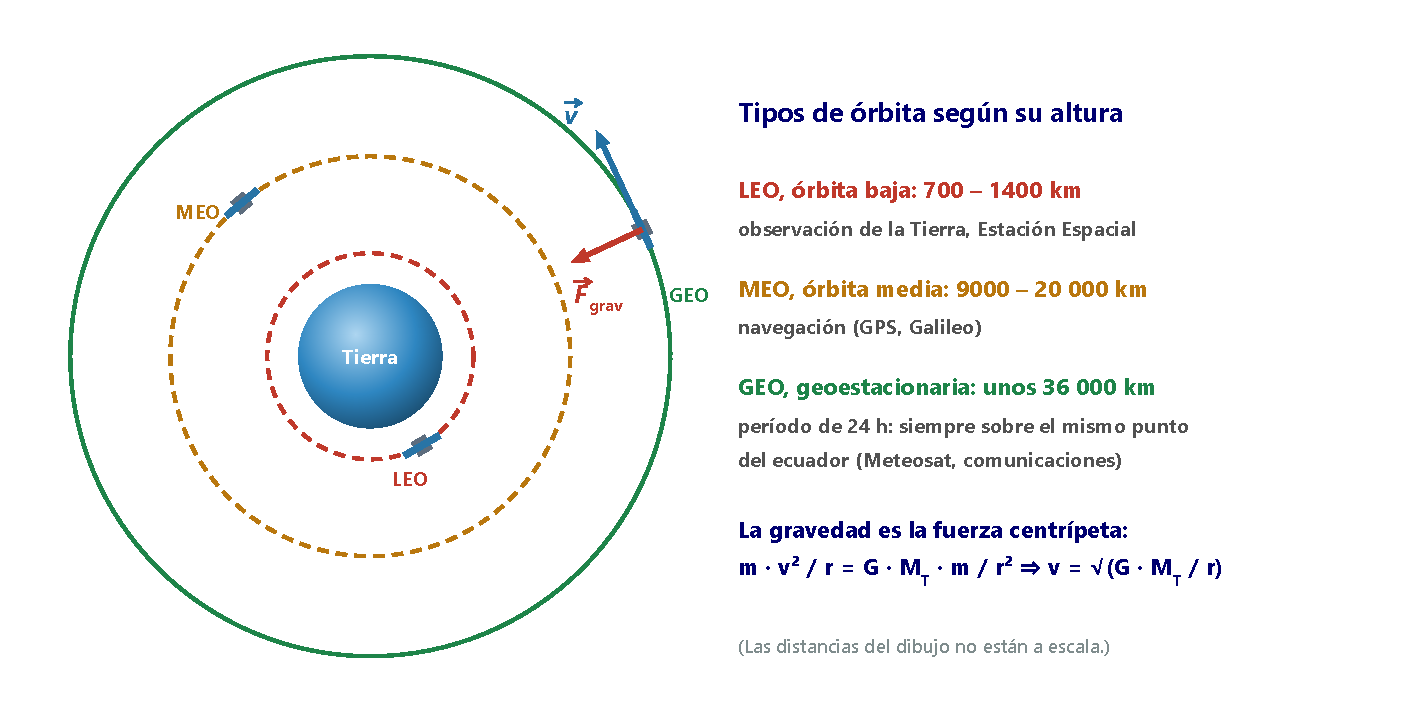
\includegraphics[width=0.8\textwidth]{images/UD11/orbitas_satelites}
    \caption{Órbitas bajas, medias y geoestacionarias. La gravedad es la fuerza centrípeta.}
    \label{fig:ud11-orbitas}
\end{figure}

\begin{example}
    \textbf{Un satélite de observación.} Calcula la velocidad y el periodo de un satélite que orbita a \qty{700}{\km} de altura.

    \textbf{Solución.} \(r = 6370 + 700 = \qty{7070}{\km}\).
    \[ v = \sqrt{\frac{\num{6.67e-11} \cdot \num{5.97e24}}{\num{7.07e6}}} = \qty{7.50e3}{\m\per\s} \qquad
    T = \frac{2\pi \cdot \num{7.07e6}}{\num{7.50e3}} = \qty{5.92e3}{\s} \approx \qty{99}{\minute} \]
\end{example}

\subsection{Coches en las curvas}

\paragraph{Curva plana.} El coche describe un arco de circunferencia y la única fuerza horizontal es el \textbf{rozamiento} lateral
entre los neumáticos y el asfalto, que hace de fuerza centrípeta; en vertical, el peso y la normal se equilibran
(figura~\ref{fig:ud11-curvas}). La velocidad máxima sin derrapar se alcanza cuando el rozamiento llega a su valor máximo:
\[ \mu\,m\,g = m\,\frac{v^2}{r} \quad\Longrightarrow\quad v_{\text{máx}} = \sqrt{\mu\,g\,r} \]

\paragraph{Curva peraltada.} Si la carretera está inclinada hacia el interior un ángulo \(\alpha\) (peralte), la normal tiene una
componente horizontal que contribuye a la fuerza centrípeta. Sin rozamiento:
\[ N\cos\alpha = m\,g \qquad N\sen\alpha = m\,\frac{v^2}{r} \quad\Longrightarrow\quad v = \sqrt{g\,r\tg\alpha} \]

\begin{figure}[H]
    \centering
    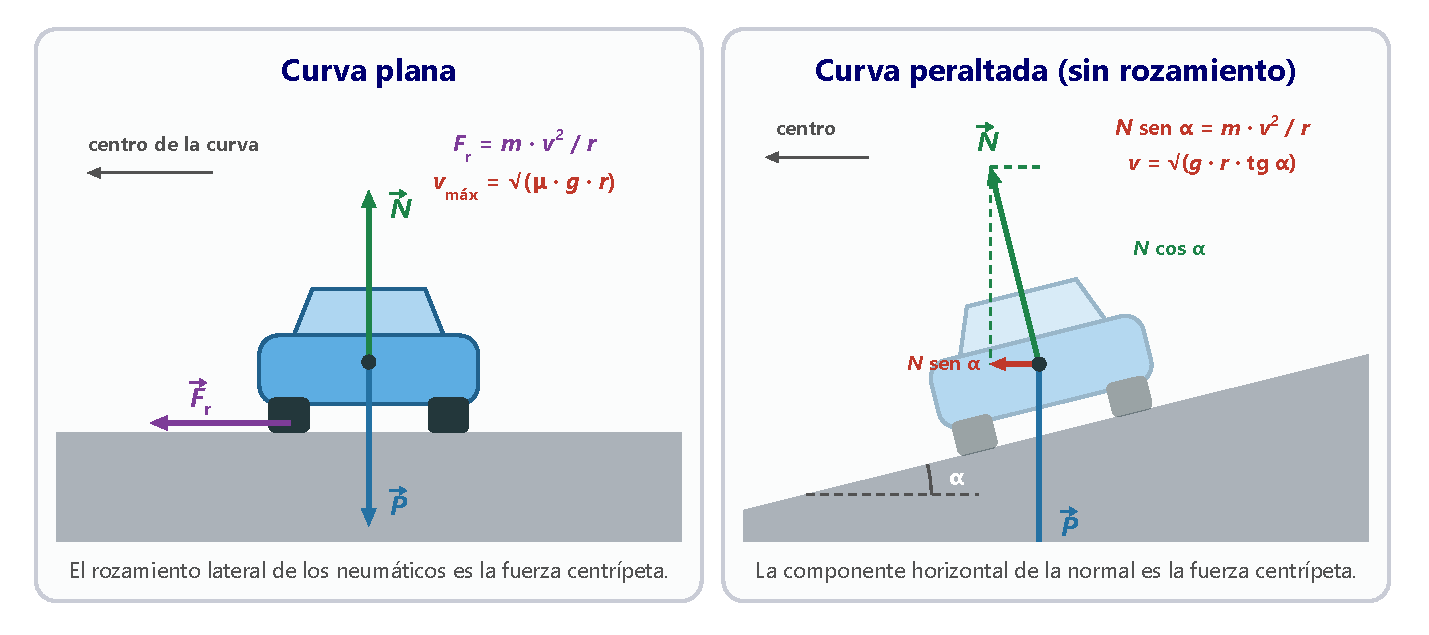
\includegraphics[width=0.95\textwidth]{images/UD11/curvas}
    \caption{Fuerzas sobre un coche en una curva plana y en una curva peraltada.}
    \label{fig:ud11-curvas}
\end{figure}

\begin{remark}
    La velocidad máxima en una curva no depende de la masa del vehículo, sino del radio y del coeficiente de rozamiento, que cambia
    mucho con el estado del asfalto y de los neumáticos (presión, desgaste) o si hay agua o hielo.
\end{remark}

\begin{example}
    \textbf{Velocidad máxima en una curva.} Una curva tiene \qty{80}{\m} de radio. Calcula la velocidad máxima: a) si es plana y el
    coeficiente de rozamiento es \num{0.6}; b) si tiene un peralte de \(10^\circ\) y no hubiera rozamiento (hielo).

    \textbf{Solución.} a) \(v = \sqrt{\num{0.6} \cdot \num{9.8} \cdot 80} = \qty{21.7}{\m\per\s}\) (\qty{78}{\km\per\hour}).
    b) \(v = \sqrt{\num{9.8} \cdot 80 \cdot \tg 10^\circ} = \qty{11.8}{\m\per\s}\) (\qty{42}{\km\per\hour}).
\end{example}

\begin{exercise}
    Un patinador de \qty{70}{\kg} recorre un circuito circular de \qty{20}{\m} de radio y está sometido a una fuerza centrípeta de
    \qty{315}{\newton}. ¿Qué velocidad lleva?
    \begin{solu}
        \(v = \sqrt{\dfrac{F_c\,r}{m}} = \sqrt{\dfrac{315 \cdot 20}{70}} = \textcolor{red}{\qty{9.49}{\m\per\s}}\).
    \end{solu}
\end{exercise}

\begin{exercise}
    Un coche teledirigido de \qty{2}{\kg} da 6 vueltas por minuto en una pista circular de \qty{1.5}{\m} de radio. ¿Qué fuerza
    centrípeta actúa sobre él?
    \begin{solu}
        \(\omega = \dfrac{6 \cdot 2\pi}{60} = \qty{0.628}{\radian\per\s}\); \(F_c = 2 \cdot \num{0.628}^2 \cdot \num{1.5} = \textcolor{red}{\qty{1.18}{\newton}}\).
    \end{solu}
\end{exercise}

\begin{exercise}
    Un cuerpo de \qty{4}{\kg} gira con MCU en una circunferencia de \qty{50}{\cm} de radio sometido a una fuerza centrípeta de
    \qty{120}{\newton}. ¿Cuánto tarda en dar una vuelta?
    \begin{solu}
        \(\omega = \sqrt{\dfrac{120}{4 \cdot \num{0.5}}} = \qty{7.75}{\radian\per\s}\); \(T = \dfrac{2\pi}{\omega} = \textcolor{red}{\qty{0.81}{\s}}\).
    \end{solu}
\end{exercise}

\begin{exercise}
    Un satélite meteorológico de \qty{2000}{\kg} está en órbita geoestacionaria, a \qty{42164}{\km} del centro de la Tierra. Calcula su
    velocidad y la fuerza centrípeta a la que está sometido.
    \begin{solu}
        \(v = \sqrt{\dfrac{G\,M_T}{r}} = \textcolor{red}{\qty{3.07e3}{\m\per\s}}\); \(F_c = \dfrac{m\,v^2}{r} = \textcolor{red}{\qty{448}{\newton}}\).
    \end{solu}
\end{exercise}

%========================================================================================
\section{Física en la vida: ¿se cumplen las leyes de la física en el cine?}\label{sec:ud11-cine}
%========================================================================================

Muchas películas de ciencia ficción son un buen laboratorio para poner a prueba lo que sabemos de dinámica.

En las batallas espaciales de muchas sagas, las naves giran inclinándose como aviones y las explosiones se oyen con estruendo. Pero en
el vacío no hay aire: el sonido no se propaga y una nave no puede «apoyarse» en el aire para girar; necesita expulsar gases en la
dirección contraria a la que quiere ir (tercera ley de Newton). Tampoco necesita mantener los motores encendidos para avanzar: por el
principio de inercia, seguiría moviéndose sin ellos.

Las películas de superhéroes ofrecen otro ejemplo clásico: el héroe atrapa en el aire a una persona que cae desde un rascacielos y la
detiene en un instante. Pero, por el teorema del impulso, frenar a una persona en muy poco tiempo exige una fuerza enorme: el «rescate»
sería tan dañino como el choque contra el suelo.

En cambio, \textit{Interstellar} (2014) contó con el asesoramiento del físico Kip Thorne, premio Nobel en 2017 por la detección de las
ondas gravitacionales. Su imagen del agujero negro Gargantúa se calculó con las ecuaciones de la relatividad general y resultó muy
parecida a la primera imagen real de un agujero negro, obtenida en 2019. El cine también puede ser una forma estupenda de divulgar la
ciencia.

\begin{exercise}
    a) Un superhéroe atrapa a una persona de \qty{60}{\kg} que cae a \qty{30}{\m\per\s} y la detiene en \qty{0.05}{\s}. ¿Qué fuerza media
    sufre la persona? ¿Cuántas veces su peso? ¿Y si la frenara en \qty{1}{\s}? b) En una película, una nave espacial gira en el vacío
    describiendo una curva cerrada con los motores apagados. ¿Es posible? c) Elegid una escena de una película y analizad si respeta las
    leyes de la dinámica.
    \begin{solu}
        a) \(F = \dfrac{60 \cdot 30}{\num{0.05}} = \textcolor{red}{\qty{3.6e4}{\newton}}\), unas \textcolor{red}{61 veces su peso}; en
        \qty{1}{\s}, \textcolor{red}{\qty{1800}{\newton}} (unas 3 veces su peso). b) \textcolor{red}{No}: para describir una curva hace
        falta una fuerza centrípeta; sin motores (y lejos de cualquier astro) la nave seguiría en línea recta. c) \textcolor{red}{Respuesta
        abierta}.
    \end{solu}
\end{exercise}

%========================================================================================
\section{Prácticas}\label{sec:ud11-practicas}
%========================================================================================

\subsection{El coeficiente de rozamiento estático con un libro}

\noindent\begin{minipage}[t]{0.48\textwidth}
    \textbf{Objetivo}
    \begin{itemize}
        \item Medir el coeficiente de rozamiento estático entre distintos objetos y la tapa de un libro.
    \end{itemize}
\end{minipage}\hfill
\begin{minipage}[t]{0.48\textwidth}
    \textbf{Material}
    \begin{itemize}
        \item Un libro grande de tapa dura, una regla, una moneda, un móvil (con y sin funda) y otros objetos pequeños.
    \end{itemize}
\end{minipage}

\begin{figure}[H]
    \centering
    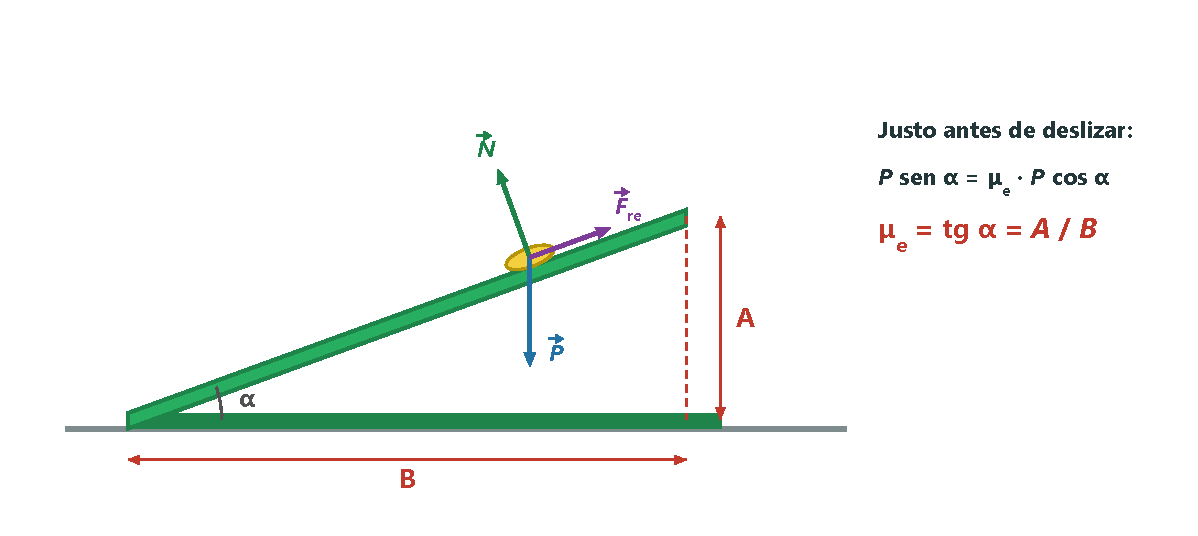
\includegraphics[width=0.75\textwidth]{images/UD11/practica_libro}
    \caption{Se levanta la tapa del libro hasta que el objeto empieza a deslizar.}
    \label{fig:ud11-libro}
\end{figure}

\textbf{Procedimiento}
\begin{enumerate}[label=\numberballgreen]
    \item Coloca el libro cerrado sobre la mesa y pon la moneda cerca del borde superior de la tapa.
    \item Levanta poco a poco la tapa hasta que la moneda empiece a deslizar. En ese momento, mide la altura \(A\) del borde de la tapa y
    la distancia horizontal \(B\) desde el lomo hasta la vertical de ese borde.
    \item Repite la medida tres veces y calcula la media. Haz lo mismo con los demás objetos.
\end{enumerate}

\begin{exercise}
    a) Demuestra que, justo cuando el objeto empieza a deslizar, \(\mu_e = \tg\alpha = A/B\). b) Con la moneda, un grupo mide
    \(A = \qty{6.2}{\cm}\) y \(B = \qty{21.0}{\cm}\); con el móvil en su funda de goma, \(A = \qty{12.8}{\cm}\) y \(B = \qty{17.5}{\cm}\).
    Calcula los coeficientes y el ángulo en el caso de la moneda. c) ¿Influye la masa del objeto? ¿Y el tamaño de la superficie de
    contacto?
    \begin{solu}
        a) \textcolor{blue}{En el límite, \(m\,g\sen\alpha = \mu_e\,m\,g\cos\alpha\).} \(\textcolor{red}{\mu_e = \tg\alpha}\), y
        \(\tg\alpha = A/B\). b) Moneda: \(\mu_e = \textcolor{red}{\num{0.30}}\) (\(\alpha = \textcolor{red}{\num{16.4}^\circ}\));
        móvil: \(\mu_e = \textcolor{red}{\num{0.73}}\). c) \textcolor{red}{No}: la masa se simplifica, y el coeficiente apenas depende del
        área de contacto; \textcolor{red}{depende de los materiales} y de lo rugosos que sean.
    \end{solu}
\end{exercise}

\subsection{Medir \texorpdfstring{\(g\)}{g} con una máquina de Atwood}

\noindent\begin{minipage}[t]{0.48\textwidth}
    \textbf{Objetivo}
    \begin{itemize}
        \item Construir una máquina de Atwood y usarla para medir la aceleración de la gravedad.
    \end{itemize}
\end{minipage}\hfill
\begin{minipage}[t]{0.48\textwidth}
    \textbf{Material}
    \begin{itemize}
        \item Una polea ligera (o el carrete de una caña de pescar), hilo resistente, dos vasos de plástico, arena o monedas, una
        balanza, una cinta métrica y un cronómetro.
    \end{itemize}
\end{minipage}

\textbf{Procedimiento}
\begin{enumerate}[label=\numberballgreen]
    \item Sujeta la polea a un soporte alto, pasa el hilo por ella y ata un vaso en cada extremo.
    \item Llena los vasos con arena hasta que tengan masas un poco distintas (por ejemplo, \qty{260}{\g} y \qty{240}{\g}).
    \item Coloca el vaso más pesado a \qty{1}{\m} del suelo, suéltalo desde el reposo y mide el tiempo que tarda en llegar al suelo.
    Repite cinco veces y calcula la media.
\end{enumerate}

\begin{exercise}
    a) Demuestra que \(g = a\,\dfrac{m_1 + m_2}{m_1 - m_2}\), con \(a = 2d/t^2\). b) Con \(m_1 = \qty{260}{\g}\), \(m_2 = \qty{240}{\g}\) y
    \(d = \qty{1.00}{\m}\), el tiempo medio es de \qty{2.27}{\s}. Calcula \(g\) y el error relativo respecto a \qty{9.8}{\m\per\s\squared}.
    c) ¿Por qué conviene que las masas sean parecidas? ¿Qué factores no hemos tenido en cuenta?
    \begin{solu}
        a) Despejando \(g\) de \(a = \dfrac{m_1 - m_2}{m_1 + m_2}\,g\). b) \(a = \dfrac{2}{\num{2.27}^2} = \qty{0.388}{\m\per\s\squared}\);
        \(g = \num{0.388} \cdot \dfrac{500}{20} = \textcolor{red}{\qty{9.70}{\m\per\s\squared}}\); error relativo \(\textcolor{red}{\qty{1}{\percent}}\).
        c) \textcolor{red}{Para que la aceleración sea pequeña y el tiempo, fácil de medir.} No hemos tenido en cuenta el
        \textcolor{red}{rozamiento de la polea, su masa ni la del hilo}.
    \end{solu}
\end{exercise}

%========================================================================================
\section{Situación de aprendizaje: satélites al servicio del planeta (ODS 17)}\label{sec:ud11-ods}
%========================================================================================

Desde que la Unión Soviética lanzó el \textbf{Sputnik 1} el 4 de octubre de 1957, el primer satélite artificial, miles de satélites
orbitan la Tierra. Hoy dependemos de ellos para las comunicaciones, la navegación por GPS y Galileo, la predicción meteorológica, la
vigilancia del medio ambiente o la respuesta ante catástrofes. Según la ONU, los datos de observación de la Tierra ayudan a cumplir
muchas de las metas de los Objetivos de Desarrollo Sostenible: permiten medir el cambio climático, detectar la contaminación del aire y
del agua o mejorar la agricultura.

La exploración del espacio es también un ejemplo del \textbf{ODS 17} (alianzas para lograr los objetivos): la Estación Espacial
Internacional es fruto de la colaboración de las agencias de Estados Unidos, Rusia, Europa, Japón y Canadá, y la Oficina de Asuntos del
Espacio Ultraterrestre de la ONU (UNOOSA) promueve el uso pacífico del espacio y lleva el registro de los objetos lanzados, para
evitar acumular más basura espacial.

\begin{marker}
    \textbf{Reto:} por grupos, preparad un mural o una presentación sobre una misión espacial europea (por ejemplo, Galileo, Copernicus,
    Meteosat de Tercera Generación o Rosetta): para qué sirve, qué órbita sigue y qué física hay detrás.
\end{marker}

\begin{enumerate}[label=\numberballred]
    \item \textbf{Investigad} qué es una órbita baja, una órbita media y una órbita geoestacionaria, y qué tipo de satélites usa cada una.
    \item \textbf{Calculad} la altura de la órbita geoestacionaria (periodo de un día sidéreo, \qty{86164}{\s}) y el periodo de la
    Estación Espacial, a \qty{420}{\km} de altura.
    \item \textbf{Analizad} el problema de la basura espacial: ¿por qué los restos se quedan en órbita durante años?
    \item \textbf{Comunicad} vuestro trabajo explicando cómo ayudan los satélites a lograr al menos tres ODS.
\end{enumerate}

\begin{exercise}
    Resuelve el apartado 2 de la situación de aprendizaje. ¿A qué velocidad se mueve un satélite geoestacionario?
    \begin{solu}
        \textcolor{blue}{De \(T = 2\pi\sqrt{r^3/(G\,M_T)}\):} \(r = \sqrt[3]{\dfrac{G\,M_T\,T^2}{4\pi^2}} = \textcolor{red}{\qty{4.22e7}{\m}}\),
        es decir, a unos \textcolor{red}{\qty{35800}{\km}} de altura; \(v = \dfrac{2\pi r}{T} = \textcolor{red}{\qty{3.07}{\km\per\s}}\).
        Estación Espacial: \(r = \qty{6.79e6}{\m}\), \(T = \textcolor{red}{\qty{92.9}{\minute}}\).
    \end{solu}
\end{exercise}

    \newpage
    %! Unidad 11 — Dinámica aplicada: ejercicios resueltos, ejercicios finales, olimpiadas y autoevaluación
%! Fuente: Fuentes/Fisica/Unidad 11 («Ejercicios resueltos», «Practica y calcula», «Piensa y resuelve») y Unidad 12 (captura 439:
%! «Olimpiadas Física» y «Autoevaluación» de este tema). Enunciados adaptados con datos cambiados (y más realistas cuando los de
%! la fuente no lo eran: rozamiento de un tren, fuerza sobre la Luna, órbitas); soluciones rehechas con g = 9,8 m/s².
%! Dificultad: \(\star\) baja, \(\star\star\) media, \(\star\star\star\) alta.

\section{Ejercicios resueltos}\label{sec:ud11-resueltos}

\begin{example}
    \textbf{Cuerpos enlazados en dos planos.} Un cuerpo de \(m_1 = \qty{4}{\kg}\) está sobre una superficie horizontal y unido por una
    cuerda, que pasa por una polea, a otro de \(m_2 = \qty{12}{\kg}\) situado en un plano inclinado \(30^\circ\). El coeficiente de
    rozamiento es \num{0.2} en ambas superficies. Calcula la aceleración del sistema y la tensión de la cuerda.

    \textbf{Solución.} \textbf{1. Datos}: \(m_1 = \qty{4}{\kg}\), \(m_2 = \qty{12}{\kg}\), \(\alpha = 30^\circ\), \(\mu = \num{0.2}\).
    \textbf{Incógnitas}: \(a\) y \(T\). El cuerpo 2 baja por el plano y arrastra al 1. Para cada cuerpo, el eje \(X\) es la dirección de su
    movimiento; la tensión es la misma en toda la cuerda y las dos aceleraciones son iguales en módulo.

    \textbf{2. Cuerpo 1}: \(N_1 = m_1\,g\); \(T - \mu\,m_1\,g = m_1\,a\) (I).

    \textbf{3. Cuerpo 2}: \(N_2 = m_2\,g\cos\alpha\); \(m_2\,g\sen\alpha - T - \mu\,m_2\,g\cos\alpha = m_2\,a\) (II).

    \textbf{4.} Sumando (I) y (II) se elimina \(T\):
    \[ a = \frac{m_2\,g\sen\alpha - \mu\,m_1\,g - \mu\,m_2\,g\cos\alpha}{m_1 + m_2} = \frac{\num{58.8} - \num{7.84} - \num{20.37}}{16}
    = \qty{1.91}{\m\per\s\squared} \]
    Con (I): \(T = m_1\,(a + \mu\,g) = 4 \cdot (\num{1.91} + \num{1.96}) = \qty{15.5}{\newton}\).
\end{example}

\begin{example}
    \textbf{Subir una cuesta.} Una calle tiene una pendiente de \(25^\circ\) (una de las más empinadas de España tiene \(27^\circ\)). Un
    coche de \qty{900}{\kg} la sube con una aceleración de \qty{0.3}{\m\per\s\squared}. Si las fuerzas de resistencia (rodadura de los
    neumáticos) equivalen a un coeficiente de \num{0.04}, ¿qué fuerza de tracción debe hacer el coche?

    \textbf{Solución.} \textbf{1.} Sobre el coche actúan el peso, la normal, la fuerza de tracción \(F\) (hacia arriba) y la
    resistencia \(F_r\) (hacia abajo). Eje \(X\) paralelo al plano, hacia arriba.

    \textbf{2.} \(P = 900 \cdot \num{9.8} = \qty{8820}{\newton}\); \(P_x = 8820\sen 25^\circ = \qty{3727}{\newton}\);
    \(N = P_y = 8820\cos 25^\circ = \qty{7994}{\newton}\); \(F_r = \num{0.04} \cdot 7994 = \qty{320}{\newton}\).

    \textbf{3.} \(F - P_x - F_r = m\,a \Rightarrow F = 900 \cdot \num{0.3} + 3727 + 320 = \qty{4317}{\newton}\). Casi toda la fuerza
    se emplea en vencer la componente del peso paralela a la cuesta.
\end{example}

\begin{example}
    \textbf{Una curva peraltada.} Una curva de autovía tiene \qty{150}{\m} de radio. a) ¿Qué peralte necesita para que un coche pueda
    tomarla a \qty{17.7}{\m\per\s} (unos \qty{64}{\km\per\hour}) aunque haya hielo? b) Si fuera plana, ¿a qué velocidad máxima se
    podría tomar con un coeficiente de rozamiento de \num{0.5}?

    \textbf{Solución.} \textbf{a)} Sin rozamiento, la componente horizontal de la normal es la fuerza centrípeta:
    \(N\sen\alpha = m\,v^2/r\) y \(N\cos\alpha = m\,g\). Dividiendo:
    \[ \tg\alpha = \frac{v^2}{g\,r} = \frac{\num{17.7}^2}{\num{9.8} \cdot 150} = \num{0.213} \Rightarrow \alpha = 12^\circ \]
    \textbf{b)} \(v_{\text{máx}} = \sqrt{\mu\,g\,r} = \sqrt{\num{0.5} \cdot \num{9.8} \cdot 150} = \qty{27.1}{\m\per\s}\)
    (\qty{98}{\km\per\hour}).
\end{example}

\begin{example}
    \textbf{Los satélites Galileo.} Los satélites del sistema europeo de navegación Galileo orbitan a \qty{23222}{\km} de altura.
    Calcula su velocidad, su periodo y la aceleración de la gravedad a esa altura.

    \textbf{Solución.} \textbf{1.} \(r = R_T + h = 6370 + 23222 = \qty{29592}{\km}\).

    \textbf{2.} La gravedad es la fuerza centrípeta: \(v = \sqrt{\dfrac{G\,M_T}{r}} = \sqrt{\dfrac{\num{6.67e-11} \cdot \num{5.97e24}}{\num{2.959e7}}}
    = \qty{3.67e3}{\m\per\s}\).

    \textbf{3.} \(T = \dfrac{2\pi r}{v} = \qty{5.07e4}{\s} = \qty{14.1}{\hour}\); \(g = \dfrac{G\,M_T}{r^2} = \qty{0.455}{\m\per\s\squared}\).
\end{example}

\begin{example}
    \textbf{Péndulo cónico.} Una bola de \qty{200}{\g} atada a un hilo de \qty{1}{\m} gira en una circunferencia horizontal de modo
    que el hilo forma \(30^\circ\) con la vertical. Calcula la tensión del hilo, la velocidad de la bola y el periodo.

    \textbf{Solución.} \textbf{1.} Sobre la bola actúan el peso y la tensión. El radio de la circunferencia es \(r = 1 \cdot \sen 30^\circ
    = \qty{0.5}{\m}\).

    \textbf{2.} Eje vertical (equilibrio): \(T\cos 30^\circ = m\,g \Rightarrow T = \dfrac{\num{0.2} \cdot \num{9.8}}{\cos 30^\circ} = \qty{2.26}{\newton}\).

    \textbf{3.} Eje radial: la componente horizontal de la tensión es la fuerza centrípeta, \(T\sen 30^\circ = m\,v^2/r\). Dividiendo
    entre la ecuación anterior: \(v = \sqrt{g\,r\tg 30^\circ} = \qty{1.68}{\m\per\s}\); \(T_{\text{periodo}} = \dfrac{2\pi r}{v} = \qty{1.87}{\s}\).
\end{example}

%========================================================================================
\section{Ejercicios de aplicación}\label{sec:ud11-aplicacion}
%========================================================================================

Datos: \(G = \qty{6.67e-11}{\newton\m\squared\per\kg\squared}\); \(M_T = \qty{5.97e24}{\kg}\); \(R_T = \qty{6370}{\km}\);
\(k = \qty{9e9}{\newton\m\squared\per\coulomb\squared}\).

\subsection{Fuerzas a distancia}

\begin{exercise}
    \(\star\star\) ¿Cuál es el peso de una persona de \qty{70}{\kg} en la superficie de la Tierra (calculado con la ley de gravitación)?
    ¿Y en la cima del Everest, a \qty{8849}{\m}? ¿Y en un satélite a \qty{36000}{\km} de la superficie?
    \begin{solu}
        \textcolor{red}{\qty{687}{\newton}}; \textcolor{red}{\qty{685}{\newton}} (apenas cambia); \textcolor{red}{\qty{15.5}{\newton}}.
    \end{solu}
\end{exercise}

\begin{exercise}
    \(\star\) Un ferry de \qty{30000}{t} navega a \qty{1.5}{\km} de un petrolero de \qty{200000}{t}. ¿Con qué fuerza gravitatoria se
    atraen?
    \begin{solu}
        \(F = \num{6.67e-11} \cdot \dfrac{\num{3e7} \cdot \num{2e8}}{1500^2} = \textcolor{red}{\qty{0.18}{\newton}}\): insignificante.
    \end{solu}
\end{exercise}

\begin{exercise}
    \(\star\) Un astronauta de \qty{90}{\kg} (con su traje) está en la Luna, donde \(g = \qty{1.62}{\m\per\s\squared}\). a) ¿Cuánto pesa?
    b) ¿Qué masa debería tener un objeto para pesar lo mismo en la Tierra?
    \begin{solu}
        a) \(P = \textcolor{red}{\qty{146}{\newton}}\). b) \(m = \dfrac{146}{\num{9.8}} = \textcolor{red}{\qty{14.9}{\kg}}\).
    \end{solu}
\end{exercise}

\begin{exercise}
    \(\star\star\) ¿Cómo cambia la fuerza de atracción gravitatoria entre dos cuerpos si: a) la distancia se triplica; b) la masa de uno de
    ellos se triplica; c) las dos masas y la distancia se multiplican por 4?
    \begin{solu}
        a) \textcolor{red}{Se divide entre 9}. b) \textcolor{red}{Se triplica}. c) \(\dfrac{4 \cdot 4}{4^2} = 1\): \textcolor{red}{no cambia}.
    \end{solu}
\end{exercise}

\begin{exercise}
    \(\star\) ¿Con qué fuerza se atraen dos hermanos de \qty{55}{\kg} y \qty{70}{\kg} situados a \qty{1.5}{\m}?
    \begin{solu}
        \(F = \textcolor{red}{\qty{1.14e-7}{\newton}}\).
    \end{solu}
\end{exercise}

\begin{exercise}
    \(\star\star\) ¿Qué semejanzas y diferencias hay entre la interacción gravitatoria y la electrostática?
    \begin{solu}
        \textcolor{red}{Semejanzas}: actúan a distancia, en la recta que une los cuerpos, y disminuyen con el cuadrado de la distancia.
        \textcolor{red}{Diferencias}: la gravitatoria depende de las masas y siempre atrae; la eléctrica depende de las cargas, puede
        atraer o repeler, es muchísimo más intensa y su constante depende del medio.
    \end{solu}
\end{exercise}

\begin{exercise}
    \(\star\) Dos cargas puntuales iguales y de signo contrario, separadas \qty{50}{\cm}, se atraen con una fuerza de \qty{10}{\newton}.
    ¿Cuánto vale cada carga?
    \begin{solu}
        \(q = \sqrt{\dfrac{10 \cdot \num{0.25}}{\num{9e9}}} = \textcolor{red}{\qty{1.67e-5}{\coulomb}}\): \textcolor{red}{\(+\num{16.7}\)
        y \(-\qty{16.7}{\micro\coulomb}\)}.
    \end{solu}
\end{exercise}

\begin{exercise}
    \(\star\) ¿A qué distancia en el vacío están dos cargas de \qty{-4}{\micro\coulomb} y \qty{+3}{\micro\coulomb} que se atraen con
    una fuerza de \qty{3}{\newton}?
    \begin{solu}
        \(r = \sqrt{\dfrac{\num{9e9} \cdot \num{12e-12}}{3}} = \textcolor{red}{\qty{0.19}{\m}}\).
    \end{solu}
\end{exercise}

\begin{exercise}
    \(\star\) ¿Con qué fuerza se atraen dos cargas de \qty{-2}{\micro\coulomb} y \qty{+5}{\micro\coulomb} situadas a \qty{30}{\cm}?
    \begin{solu}
        \(F = \num{9e9} \cdot \dfrac{\num{1e-11}}{\num{0.09}} = \textcolor{red}{\qty{1}{\newton}}\).
    \end{solu}
\end{exercise}

\begin{exercise}
    \(\star\star\) Dos cargas de \qty{-5}{\micro\coulomb} y \qty{+8}{\micro\coulomb} están separadas \qty{1}{\m}. Entre ellas, a
    \qty{40}{\cm} de la primera, hay una carga de \qty{+2}{\micro\coulomb}. ¿Qué fuerza total actúa sobre ella?
    \begin{solu}
        \textcolor{blue}{La primera la atrae (hacia ella): \qty{0.5625}{\newton}; la segunda la repele (también hacia la primera):
        \qty{0.40}{\newton}.} \(F = \textcolor{red}{\qty{0.96}{\newton}}\), \textcolor{red}{hacia la carga de \qty{-5}{\micro\coulomb}}.
    \end{solu}
\end{exercise}

\begin{exercise}
    \(\star\star\star\) Tres cargas iguales de \qty{+2}{\micro\coulomb} están en los vértices de un triángulo rectángulo isósceles. Sobre
    la carga del ángulo recto actúa una fuerza de \qty{1.5}{\newton}. ¿Cuánto miden los catetos?
    \begin{solu}
        \textcolor{blue}{Las dos fuerzas son iguales y perpendiculares:} \(F = \sqrt{2}\,F_0\), así que \(F_0 = \qty{1.06}{\newton}\).
        \(L = \sqrt{\dfrac{\num{9e9} \cdot (\num{2e-6})^2}{\num{1.06}}} = \textcolor{red}{\qty{0.18}{\m}}\).
    \end{solu}
\end{exercise}

\subsection{Fuerzas de contacto}

\begin{exercise}
    \(\star\star\) Explica con tus palabras qué son la fuerza normal, la fuerza de rozamiento y la tensión, y pon un ejemplo de cada una.
    \begin{solu}
        \textcolor{red}{Normal}: la que hace una superficie sobre un cuerpo apoyado (el suelo sobre nuestros pies). \textcolor{red}{Rozamiento}:
        se opone al deslizamiento (frena un trineo). \textcolor{red}{Tensión}: la que transmite una cuerda tensa (la cadena de un columpio).
    \end{solu}
\end{exercise}

\begin{exercise}
    \(\star\star\) Calcula la fuerza de rozamiento sobre un cuerpo de \qty{4}{\kg} cuando: a) se arrastra por un plano horizontal;
    b) desciende por un plano inclinado \(30^\circ\); c) asciende por un plano inclinado \(40^\circ\). En todos los casos, \(\mu = \num{0.3}\).
    \begin{solu}
        a) \textcolor{red}{\qty{11.8}{\newton}}. b) \(\num{0.3} \cdot \num{39.2}\cos 30^\circ = \textcolor{red}{\qty{10.2}{\newton}}\).
        c) \(\num{0.3} \cdot \num{39.2}\cos 40^\circ = \textcolor{red}{\qty{9.0}{\newton}}\).
    \end{solu}
\end{exercise}

\begin{exercise}
    \(\star\) Un ordenador de \qty{2}{\kg} está sobre una mesa. a) ¿Qué fuerzas actúan sobre él? b) Si tiramos de él verticalmente
    hacia arriba con una cuerda con una fuerza de \qty{6}{\newton}, ¿cuánto vale la normal?
    \begin{solu}
        a) \textcolor{red}{El peso y la normal}, iguales: \qty{19.6}{\newton}. b) \(N = \num{19.6} - 6 = \textcolor{red}{\qty{13.6}{\newton}}\).
    \end{solu}
\end{exercise}

\begin{exercise}
    \(\star\star\) Una mesa de \qty{20}{\kg} está en reposo sobre el suelo; \(\mu_e = \num{0.45}\) y \(\mu_c = \num{0.30}\). Calcula:
    a) la fuerza horizontal mínima para moverla; b) la fuerza de rozamiento si se empuja con \qty{120}{\newton}; c) la aceleración.
    \begin{solu}
        a) \textcolor{red}{\qty{88.2}{\newton}}. b) Se mueve: \(F_r = \textcolor{red}{\qty{58.8}{\newton}}\). c) \(a = \textcolor{red}{\qty{3.06}{\m\per\s\squared}}\).
    \end{solu}
\end{exercise}

\begin{exercise}
    \(\star\star\) Para colgar un cuadro de \qty{3}{\kg}, lo apretamos contra la pared con una fuerza de \qty{40}{\newton}. Si
    \(\mu_e = \num{0.4}\): a) ¿se caerá? b) ¿Qué fuerza normal hace la pared?
    \begin{solu}
        a) \(F_{re,\,\text{máx}} = \num{0.4} \cdot 40 = \qty{16}{\newton}\), menor que el peso (\qty{29.4}{\newton}): \textcolor{red}{se cae}.
        b) \textcolor{red}{\qty{40}{\newton}}.
    \end{solu}
\end{exercise}

\begin{exercise}
    \(\star\star\) Un ascensor de \qty{700}{\kg} sube a una pareja que suma \qty{200}{\kg} con una aceleración de \qty{1.5}{\m\per\s\squared}.
    Calcula la tensión del cable y la fuerza que hace el suelo sobre la pareja.
    \begin{solu}
        \(T = 900 \cdot \num{11.3} = \textcolor{red}{\qty{10170}{\newton}}\); \(N = 200 \cdot \num{11.3} = \textcolor{red}{\qty{2260}{\newton}}\).
    \end{solu}
\end{exercise}

\begin{exercise}
    \(\star\star\) Una niña arrastra con una cuerda horizontal una carretilla de \qty{5}{\kg} con una aceleración de \qty{2}{\m\per\s\squared}.
    Si \(\mu = \num{0.2}\): a) ¿cuánto valen la tensión de la cuerda y el rozamiento? b) Si la cuerda forma \(30^\circ\) con la horizontal
    y la tensión es la misma, ¿cuánto vale ahora el rozamiento?
    \begin{solu}
        a) \(F_r = \textcolor{red}{\qty{9.8}{\newton}}\); \(T = 5 \cdot 2 + \num{9.8} = \textcolor{red}{\qty{19.8}{\newton}}\).
        b) \(N = 49 - \num{19.8}\sen 30^\circ = \qty{39.1}{\newton}\): \(F_r = \textcolor{red}{\qty{7.8}{\newton}}\).
    \end{solu}
\end{exercise}

\begin{exercise}
    \(\star\) Enuncia la ley de Hooke y pon ejemplos de la vida cotidiana en que se aplique. ¿Qué es un dinamómetro?
    \begin{solu}
        \textcolor{red}{La fuerza elástica es proporcional a la deformación: \(F = -k\,\Delta L\).} Ejemplos: la suspensión de un coche,
        un colchón de muelles, una báscula de baño. El \textcolor{red}{dinamómetro} es un muelle con una escala que mide fuerzas.
    \end{solu}
\end{exercise}

\begin{exercise}
    \(\star\star\) Una persona de \qty{75}{\kg} hace \textit{puenting} con una cuerda elástica de \qty{12}{\m}. Cuando, al final, queda
    colgada en reposo, la cuerda mide \qty{20}{\m}. ¿Cuál es su constante elástica?
    \begin{solu}
        \(k = \dfrac{75 \cdot \num{9.8}}{8} = \textcolor{red}{\qty{91.9}{\newton\per\m}}\).
    \end{solu}
\end{exercise}

\begin{exercise}
    \(\star\star\) Al colgar \qty{600}{\g} de un muelle M, este se estira \qty{6}{\cm}; al colgarlos de otro muelle N, \qty{15}{\cm}.
    Calcula sus constantes. ¿Cuál es más rígido?
    \begin{solu}
        \(k_M = \textcolor{red}{\qty{98}{\newton\per\m}}\); \(k_N = \textcolor{red}{\qty{39.2}{\newton\per\m}}\). \textcolor{red}{El M}.
    \end{solu}
\end{exercise}

\begin{exercise}
    \(\star\star\) Un muelle se alarga \qty{5}{\cm} cuando le colgamos \qty{4}{\kg}. a) Calcula su constante. b) ¿Qué masa lo alargaría
    \qty{12}{\cm}?
    \begin{solu}
        a) \(k = \textcolor{red}{\qty{784}{\newton\per\m}}\). b) \(m = \dfrac{784 \cdot \num{0.12}}{\num{9.8}} = \textcolor{red}{\qty{9.6}{\kg}}\).
    \end{solu}
\end{exercise}

\subsection{Dinámica del movimiento rectilíneo}

\begin{exercise}
    \(\star\star\) Queremos mover un mueble de \qty{30}{\kg} con una fuerza de \qty{200}{\newton}. Sin rozamiento, calcula la aceleración si
    la fuerza: a) es horizontal; b) forma \(30^\circ\) sobre la horizontal; c) forma \(20^\circ\) bajo la horizontal.
    \begin{solu}
        a) \textcolor{red}{\qty{6.67}{\m\per\s\squared}}. b) \textcolor{red}{\qty{5.77}{\m\per\s\squared}}. c) \textcolor{red}{\qty{6.26}{\m\per\s\squared}}.
    \end{solu}
\end{exercise}

\begin{exercise}
    \(\star\star\) A un cuerpo de \qty{50}{\kg}, en reposo sobre una superficie horizontal, se le aplica durante \qty{6}{\s} una fuerza
    de \qty{250}{\newton} que forma \(30^\circ\) sobre la horizontal. Si \(\mu = \num{0.25}\), calcula la aceleración y la velocidad final.
    \begin{solu}
        \(N = 490 - 125 = \qty{365}{\newton}\); \(F_r = \qty{91.3}{\newton}\); \(a = \dfrac{\num{216.5} - \num{91.3}}{50} =
        \textcolor{red}{\qty{2.51}{\m\per\s\squared}}\); \(v = \textcolor{red}{\qty{15.0}{\m\per\s}}\).
    \end{solu}
\end{exercise}

\begin{exercise}
    \(\star\star\) Un esquiador de \qty{80}{\kg} baja por una pista inclinada \(30^\circ\) con una aceleración de \qty{4.0}{\m\per\s\squared}.
    Calcula: a) el coeficiente de rozamiento; b) la distancia que recorre y la altura que desciende en \qty{5}{\s}, partiendo del reposo;
    c) la variación de su momento lineal en ese tiempo.
    \begin{solu}
        a) \(\mu = \dfrac{g\sen 30^\circ - a}{g\cos 30^\circ} = \textcolor{red}{\num{0.11}}\). b) \(d = \textcolor{red}{\qty{50}{\m}}\);
        \(h = 50\sen 30^\circ = \textcolor{red}{\qty{25}{\m}}\). c) \(\Delta p = 80 \cdot 20 = \textcolor{red}{\qty{1600}{\kg\m\per\s}}\).
    \end{solu}
\end{exercise}

\begin{exercise}
    \(\star\star\) Un cuerpo de \qty{3}{\kg} desciende por un plano inclinado \(25^\circ\) con \(\mu = \num{0.2}\). a) Dibuja las fuerzas.
    b) Calcula su aceleración.
    \begin{solu}
        b) \(a = g\,(\sen 25^\circ - \num{0.2}\cos 25^\circ) = \textcolor{red}{\qty{2.37}{\m\per\s\squared}}\) (no depende de la masa).
    \end{solu}
\end{exercise}

\begin{exercise}
    \(\star\star\) a) Calcula la aceleración de un cuerpo de \qty{25}{\kg} que desciende por un plano inclinado \(35^\circ\) con
    \(\mu = \num{0.3}\). b) Si, ya en la base, lo subimos aplicándole una fuerza de \qty{260}{\newton} paralela al plano, ¿con qué
    aceleración sube?
    \begin{solu}
        a) \(a = \textcolor{red}{\qty{3.21}{\m\per\s\squared}}\). b) \(a = \dfrac{260 - \num{140.5} - \num{60.2}}{25} = \textcolor{red}{\qty{2.37}{\m\per\s\squared}}\).
    \end{solu}
\end{exercise}

\subsection{Cuerpos enlazados}

\begin{exercise}
    \(\star\star\) Un tren de mercancías está formado por una locomotora de \qty{20}{t} y tres vagones de \qty{10}{t} cada uno, y
    arranca con una aceleración de \qty{0.5}{\m\per\s\squared}. Si el coeficiente de rozamiento por rodadura es \num{0.005}, calcula la
    fuerza de tracción de la locomotora y la tensión del enganche entre la locomotora y el primer vagón.
    \begin{solu}
        \(F = \num{50000} \cdot (\num{0.5} + \num{0.005} \cdot \num{9.8}) = \textcolor{red}{\qty{2.75e4}{\newton}}\);
        \(T = \num{30000} \cdot \num{0.549} = \textcolor{red}{\qty{1.65e4}{\newton}}\).
    \end{solu}
\end{exercise}

\begin{exercise}
    \(\star\star\) Dos bloques de madera, A de \qty{3}{\kg} y B de \qty{5}{\kg}, están unidos por una cuerda sobre una superficie sin
    rozamiento. Tiramos de A y el conjunto adquiere una aceleración de \qty{1.5}{\m\per\s\squared}. ¿Con qué fuerza tiramos? ¿Cuál es la
    tensión de la cuerda?
    \begin{solu}
        \(F = 8 \cdot \num{1.5} = \textcolor{red}{\qty{12}{\newton}}\); \(T = 5 \cdot \num{1.5} = \textcolor{red}{\qty{7.5}{\newton}}\).
    \end{solu}
\end{exercise}

\begin{exercise}
    \(\star\star\) Se saca agua de un pozo con un cubo de \qty{6}{\kg} que sube con una aceleración de \qty{0.5}{\m\per\s\squared}.
    ¿Cuánto vale la tensión de la cuerda?
    \begin{solu}
        \(T = 6 \cdot (\num{9.8} + \num{0.5}) = \textcolor{red}{\qty{61.8}{\newton}}\).
    \end{solu}
\end{exercise}

\begin{exercise}
    \(\star\star\) En una máquina de Atwood cuelgan dos cuerpos de \qty{10}{\kg}. ¿Qué masa hay que añadir a uno de ellos para que el
    conjunto alcance una velocidad de \qty{2}{\m\per\s} en \qty{1.5}{\s}, partiendo del reposo?
    \begin{solu}
        \(a = \qty{1.33}{\m\per\s\squared}\); \(\Delta m\,g = (20 + \Delta m)\,a \Rightarrow \Delta m = \dfrac{20 \cdot \num{1.33}}{\num{9.8} - \num{1.33}}
        = \textcolor{red}{\qty{3.15}{\kg}}\).
    \end{solu}
\end{exercise}

\begin{exercise}
    \(\star\star\) De los extremos de una cuerda que pasa por una polea cuelgan dos cuerpos de \qty{600}{\g} y \qty{1.5}{\kg}. Calcula
    la aceleración del sistema y la tensión de la cuerda.
    \begin{solu}
        \(a = \dfrac{\num{0.9}}{\num{2.1}} \cdot \num{9.8} = \textcolor{red}{\qty{4.2}{\m\per\s\squared}}\); \(T = \num{0.6} \cdot (\num{9.8} + \num{4.2})
        = \textcolor{red}{\qty{8.4}{\newton}}\).
    \end{solu}
\end{exercise}

\begin{exercise}
    \(\star\star\star\) Dos cuerpos de \(m_1 = \qty{10}{\kg}\) y \(m_2 = \qty{20}{\kg}\) están en las dos caras de un tejado de dos aguas,
    inclinadas \(30^\circ\) y \(45^\circ\) respectivamente, unidos por una cuerda que pasa por una polea en el vértice. Con \(\mu = \num{0.2}\)
    en ambas caras, calcula la aceleración.
    \begin{solu}
        \textcolor{blue}{Baja \(m_2\).} \(P_{2x} = \qty{138.6}{\newton}\) y \(P_{1x} = \qty{49.0}{\newton}\); los rozamientos suman
        \qty{44.7}{\newton}.
        \[ a = \frac{\num{138.6} - 49 - \num{44.7}}{30} = \textcolor{red}{\qty{1.50}{\m\per\s\squared}} \]
    \end{solu}
\end{exercise}

\subsection{Dinámica del movimiento circular}

\begin{exercise}
    \(\star\) ¿Qué fuerza hace de fuerza centrípeta en cada caso? a) La Luna alrededor de la Tierra. b) Un coche en una curva plana.
    c) Una piedra atada a una cuerda. d) Un electrón alrededor del núcleo (en el modelo de Bohr).
    \begin{solu}
        a) \textcolor{red}{La gravitatoria}. b) \textcolor{red}{El rozamiento}. c) \textcolor{red}{La tensión}. d) \textcolor{red}{La
        electrostática}.
    \end{solu}
\end{exercise}

\begin{exercise}
    \(\star\star\) Con una honda hacemos girar una piedra de \qty{200}{\g} a 2 vueltas por segundo en una circunferencia de \qty{80}{\cm}
    de radio. ¿Cuál es la fuerza centrípeta?
    \begin{solu}
        \(\omega = 4\pi~\unit{\radian\per\s}\); \(F_c = \num{0.2} \cdot (4\pi)^2 \cdot \num{0.8} = \textcolor{red}{\qty{25.3}{\newton}}\).
    \end{solu}
\end{exercise}

\begin{exercise}
    \(\star\star\) Un patinador de \qty{70}{\kg} hace un \textit{looping} de \qty{4}{\m} de radio. En el punto más alto su velocidad es de
    \qty{25}{\km\per\hour}. Calcula: a) su aceleración en ese punto; b) la fuerza normal; c) la velocidad mínima para no caer.
    \begin{solu}
        a) \(a_t = 0\) y \(a_n = \dfrac{\num{6.94}^2}{4} = \textcolor{red}{\qty{12.1}{\m\per\s\squared}}\). b) Arriba, el peso y la normal
        apuntan al centro: \(N = m\,a_n - m\,g = \textcolor{red}{\qty{158}{\newton}}\). c) Con \(N = 0\): \(v = \sqrt{g\,r} = \textcolor{red}{\qty{6.26}{\m\per\s}}\).
    \end{solu}
\end{exercise}

\begin{exercise}
    \(\star\star\) Un tren de juguete de \qty{600}{\g} recorre una pista circular de \qty{1.5}{\m} de radio a \qty{0.8}{\m\per\s}. Calcula
    su aceleración y la fuerza centrípeta.
    \begin{solu}
        \(a_c = \textcolor{red}{\qty{0.43}{\m\per\s\squared}}\); \(F_c = \textcolor{red}{\qty{0.26}{\newton}}\).
    \end{solu}
\end{exercise}

\begin{exercise}
    \(\star\star\) Un satélite de comunicaciones de \qty{4500}{\kg} está sometido a una fuerza gravitatoria de \qty{1000}{\newton}. ¿A
    qué distancia del centro de la Tierra está? ¿Con qué velocidad orbita?
    \begin{solu}
        \(r = \sqrt{\dfrac{G\,M_T\,m}{F}} = \textcolor{red}{\qty{4.23e7}{\m}}\) (casi la órbita geoestacionaria); \(v = \textcolor{red}{\qty{3.07e3}{\m\per\s}}\).
    \end{solu}
\end{exercise}

\begin{exercise}
    \(\star\star\) ¿A qué velocidad máxima puede tomarse una curva plana de \qty{50}{\m} de radio si el coeficiente de rozamiento es \num{0.7}?
    \begin{solu}
        \(v = \sqrt{\num{0.7} \cdot \num{9.8} \cdot 50} = \textcolor{red}{\qty{18.5}{\m\per\s}}\) (\qty{67}{\km\per\hour}).
    \end{solu}
\end{exercise}

\begin{exercise}
    \(\star\star\) Una curva de \qty{120}{\m} de radio tiene un peralte de \(15^\circ\). ¿A qué velocidad se puede tomar sin necesidad de
    rozamiento?
    \begin{solu}
        \(v = \sqrt{\num{9.8} \cdot 120 \cdot \tg 15^\circ} = \textcolor{red}{\qty{17.8}{\m\per\s}}\) (\qty{64}{\km\per\hour}).
    \end{solu}
\end{exercise}

\begin{exercise}
    \(\star\star\) La Luna está a \qty{3.84e8}{\m} del centro de la Tierra. Calcula su periodo orbital a partir de la ley de gravitación.
    \begin{solu}
        \(T = 2\pi\sqrt{\dfrac{r^3}{G\,M_T}} = \qty{2.37e6}{\s} = \textcolor{red}{\num{27.4}~\text{días}}\).
    \end{solu}
\end{exercise}

%========================================================================================
\section{Ejercicios de ampliación}\label{sec:ud11-ampliacion}
%========================================================================================

\begin{exercise}
    \(\star\star\) En un eclipse total de Luna, el Sol, la Tierra y la Luna están alineados en ese orden. Calcula la fuerza gravitatoria
    total sobre la Luna. (Distancia Tierra-Sol: \qty{1.5e8}{\km}; Tierra-Luna: \qty{3.84e5}{\km}; \(M_L = \qty{7.35e22}{\kg}\);
    \(M_S = \qty{1.99e30}{\kg}\).)
    \begin{solu}
        \textcolor{blue}{Las dos fuerzas apuntan hacia el Sol: \(F_{TL} = \qty{1.98e20}{\newton}\) y \(F_{SL} = \qty{4.31e20}{\newton}\).}
        \(F = \textcolor{red}{\qty{6.3e20}{\newton}}\), \textcolor{red}{dirigida hacia el Sol (y la Tierra)}.
    \end{solu}
\end{exercise}

\begin{exercise}
    \(\star\star\star\) En los vértices de un triángulo equilátero de \qty{40}{\cm} de lado hay tres cargas de \qty{+2}{\micro\coulomb}.
    ¿Qué fuerza actúa sobre una carga de \qty{+1}{\micro\coulomb} situada en el centro del triángulo? ¿Y si está en el punto medio de
    un lado?
    \begin{solu}
        \textcolor{red}{En el centro, cero} (por simetría). En el punto medio de un lado se anulan las de los extremos de ese lado y queda
        la del vértice opuesto, a \(\num{0.4}\sen 60^\circ = \qty{0.346}{\m}\): \(F = \textcolor{red}{\qty{0.15}{\newton}}\).
    \end{solu}
\end{exercise}

\begin{exercise}
    \(\star\star\star\) Un mago quiere quitar el mantel de una mesa sin mover la vajilla, que tiene una masa total de \qty{1.6}{\kg}. El
    mantel tiene \qty{300}{\g} y el coeficiente de rozamiento (vajilla-mantel y mantel-mesa) es \num{0.15}. ¿Qué fuerza mínima debe hacer
    para que la vajilla resbale sobre el mantel?
    \begin{solu}
        \textcolor{blue}{La vajilla puede acelerar como mucho \(\mu\,g\); el mantel debe acelerar más. Sobre el mantel:
        \(F - \mu\,m_v\,g - \mu\,(m_v + m_m)\,g = m_m\,a\), con \(a = \mu\,g\).}
        \(F = \mu\,g\,(2m_v + 2m_m) = \textcolor{red}{\qty{5.6}{\newton}}\) (y cuanto más rápido el tirón, mejor).
    \end{solu}
\end{exercise}

\begin{exercise}
    \(\star\star\star\) En la base de un plano inclinado \(30^\circ\) sin rozamiento hay un muelle de constante \qty{5000}{\newton\per\m}
    comprimido por un cuerpo de \qty{20}{\kg} en equilibrio. a) ¿Cuánto está comprimido? b) Si lo comprimimos \qty{3}{\cm} más y lo
    soltamos, ¿qué aceleración tiene el cuerpo en ese instante?
    \begin{solu}
        a) \(\Delta L = \dfrac{20 \cdot \num{9.8}\sen 30^\circ}{5000} = \textcolor{red}{\qty{1.96}{\cm}}\).
        b) \(F = 5000 \cdot \num{0.0496} = \qty{248}{\newton}\): \(a = \dfrac{248 - 98}{20} = \textcolor{red}{\qty{7.5}{\m\per\s\squared}}\), hacia arriba.
    \end{solu}
\end{exercise}

\begin{exercise}
    \(\star\star\star\) Dos cuerpos de \(m_1 = \qty{6}{\kg}\) y \(m_2 = \qty{4}{\kg}\) bajan por un plano inclinado \(35^\circ\) unidos por
    una cuerda tensa; \(m_1\) va delante (más abajo). Los coeficientes de rozamiento son \num{0.3} para \(m_1\) y \num{0.5} para \(m_2\).
    Calcula la aceleración y la tensión.
    \begin{solu}
        \[ a = g\left[\sen 35^\circ - \frac{\num{0.3} \cdot 6 + \num{0.5} \cdot 4}{10}\cos 35^\circ\right] = \textcolor{red}{\qty{2.57}{\m\per\s\squared}} \]
        \[ T = m_1\,(g\sen 35^\circ - \num{0.3}\,g\cos 35^\circ - a) = \textcolor{red}{\qty{3.9}{\newton}} \]
    \end{solu}
\end{exercise}

\begin{exercise}
    \(\star\star\star\) Una maleta de \qty{8}{\kg} cae sin rozamiento por la rampa de descarga de un avión, de \qty{3}{\m} de altura e
    inclinada \(35^\circ\), y sigue por una pista horizontal con \(\mu = \num{0.4}\). Calcula: a) la velocidad al final de la rampa; b) la
    distancia que recorre en la pista hasta pararse.
    \begin{solu}
        a) Rampa de \(3/\sen 35^\circ = \qty{5.23}{\m}\) con \(a = g\sen 35^\circ = \qty{5.62}{\m\per\s\squared}\): \(v = \textcolor{red}{\qty{7.67}{\m\per\s}}\).
        b) \(a = -\mu\,g = \qty{-3.92}{\m\per\s\squared}\): \(d = \dfrac{\num{7.67}^2}{2 \cdot \num{3.92}} = \textcolor{red}{\qty{7.5}{\m}}\).
    \end{solu}
\end{exercise}

\begin{exercise}
    \(\star\star\star\) Un coche de carreras toma una curva de \qty{200}{\m} de radio; \(\mu = \num{0.8}\). Calcula la velocidad máxima:
    a) si la curva es plana; b) si tiene un peralte de \(10^\circ\). (En b, con rozamiento: \(v = \sqrt{g\,r\,\dfrac{\sen\alpha + \mu\cos\alpha}{\cos\alpha - \mu\sen\alpha}}\).)
    \begin{solu}
        a) \(v = \textcolor{red}{\qty{39.6}{\m\per\s}}\) (\qty{143}{\km\per\hour}). b) \(v = \textcolor{red}{\qty{47.2}{\m\per\s}}\) (\qty{170}{\km\per\hour}).
    \end{solu}
\end{exercise}

\begin{exercise}
    \(\star\star\) De un dinamómetro sujeto al techo de un ascensor cuelga una masa de \qty{2}{\kg}, y el dinamómetro marca
    \qty{23}{\newton}. ¿Cuál es la aceleración del ascensor? ¿Puede saberse si sube o baja?
    \begin{solu}
        \(T - m\,g = m\,a \Rightarrow a = \textcolor{red}{\qty{1.7}{\m\per\s\squared}}\) hacia arriba. \textcolor{red}{No}: puede subir
        acelerando o bajar frenando.
    \end{solu}
\end{exercise}

\begin{exercise}
    \(\star\star\star\) Hacemos girar en un plano vertical un cubo con agua atado a una cuerda; la distancia del agua al hombro es de
    \qty{90}{\cm}. ¿Con qué velocidad mínima debe pasar por el punto más alto para que el agua no caiga?
    \begin{solu}
        \textcolor{blue}{En el límite, el peso es toda la fuerza centrípeta: \(m\,g = m\,v^2/r\).} \(v = \sqrt{g\,r} = \textcolor{red}{\qty{2.97}{\m\per\s}}\).
    \end{solu}
\end{exercise}

\begin{exercise}
    \(\star\star\star\) Una caja va suelta en la plataforma de un camión. Si el coeficiente de rozamiento estático entre la caja y la
    plataforma es \num{0.4}, ¿con qué aceleración máxima puede frenar el camión sin que la caja deslice?
    \begin{solu}
        \textcolor{blue}{El rozamiento estático es la única fuerza horizontal sobre la caja: \(\mu_e\,m\,g = m\,a_{\text{máx}}\).}
        \(a_{\text{máx}} = \textcolor{red}{\qty{3.92}{\m\per\s\squared}}\).
    \end{solu}
\end{exercise}

%========================================================================================
\section{Olimpiadas de Física}\label{sec:ud11-olimpiadas}
%========================================================================================

\begin{exercise}
    (Córdoba 2020) Un cuerpo de masa \(m\) desliza por un plano inclinado un ángulo \(\alpha\). Parte con una velocidad \(v_0\) hacia abajo
    desde una altura \(h\) sobre la base del plano. Determina el coeficiente de rozamiento mínimo para que el cuerpo no llegue a la base.
    Expresa el resultado en función de \(g\), \(\alpha\), \(h\) y \(v_0\).
    \begin{solu}
        \textcolor{blue}{Para frenar, el rozamiento debe superar a \(P_x\): \(a = -g\,(\mu\cos\alpha - \sen\alpha)\). Debe pararse antes de
        recorrer \(L = h/\sen\alpha\): \(v_0^2 = 2\,g\,(\mu\cos\alpha - \sen\alpha)\,L\).}
        \(\textcolor{red}{\mu_{\text{mín}} = \tg\alpha + \dfrac{v_0^2\sen\alpha}{2\,g\,h\cos\alpha}}\) (no depende de \(m\)).
    \end{solu}
\end{exercise}

\begin{exercise}
    (Valencia 2022, adaptado) Un cuerpo de \(m_1 = \qty{5}{\kg}\) está en un plano inclinado \(30^\circ\) y está unido por una cuerda que
    pasa por una polea a otro de \(m_2 = \qty{2}{\kg}\) apoyado en una superficie horizontal. Entre \(m_1\) y el plano el coeficiente de
    rozamiento es \num{0.15}; entre \(m_2\) y la superficie no hay rozamiento. El sistema se suelta desde el reposo. a) Dibuja las
    fuerzas y escribe las ecuaciones de cada cuerpo. b) Calcula la aceleración y la tensión. c) Si hubiera rozamiento entre \(m_2\) y la
    superficie, ¿a partir de qué coeficiente no se movería el sistema?
    \begin{solu}
        a) \(m_1\): \(m_1\,g\sen\alpha - \mu_1\,m_1\,g\cos\alpha - T = m_1\,a\); \(m_2\): \(T = m_2\,a\).
        b) \[ a = \frac{m_1\,g\,(\sen\alpha - \mu_1\cos\alpha)}{m_1 + m_2} = \textcolor{red}{\qty{2.59}{\m\per\s\squared}} \qquad
        T = m_2\,a = \textcolor{red}{\qty{5.18}{\newton}} \] c) No se mueve si \(\mu_2\,m_2\,g \geq m_1\,g\,(\sen\alpha - \mu_1\cos\alpha)\), es
        decir, si \(\textcolor{red}{\mu_2 \geq \num{0.93}}\).
    \end{solu}
\end{exercise}

%========================================================================================
\section{Autoevaluación}\label{sec:ud11-autoevaluacion}
%========================================================================================

\begin{exercise}
    ¿Cuál es la fuerza gravitatoria entre dos cuerpos de \qty{150}{\kg} y \qty{220}{\kg} separados \qty{60}{\cm}? ¿Y si la distancia se
    reduce a la mitad?
    \begin{solu}
        \(F = \textcolor{red}{\qty{6.11e-6}{\newton}}\); a la mitad de distancia, cuatro veces más: \textcolor{red}{\qty{2.45e-5}{\newton}}.
    \end{solu}
\end{exercise}

\begin{exercise}
    Dos cargas iguales de \qty{3}{\micro\coulomb} se repelen con una fuerza de \qty{0.4}{\newton}. ¿A qué distancia están?
    \begin{solu}
        \(r = \sqrt{\dfrac{\num{9e9} \cdot \num{9e-12}}{\num{0.4}}} = \textcolor{red}{\qty{0.45}{\m}}\).
    \end{solu}
\end{exercise}

\begin{exercise}
    El rozamiento es muy importante en nuestra vida. Pon tres ejemplos y justifica su importancia.
    \begin{solu}
        \textcolor{red}{Respuesta abierta}: caminar (los pies empujan el suelo sin resbalar), frenar un coche, sujetar objetos con la
        mano, que los clavos y tornillos no se suelten\dots
    \end{solu}
\end{exercise}

\begin{exercise}
    Un cuerpo de \qty{10}{\kg} se mueve por un plano horizontal empujado por una fuerza horizontal de \qty{70}{\newton}. Si
    \(\mu = \num{0.3}\), ¿con qué aceleración se mueve? Dibuja las fuerzas.
    \begin{solu}
        \(a = \dfrac{70 - \num{29.4}}{10} = \textcolor{red}{\qty{4.06}{\m\per\s\squared}}\).
    \end{solu}
\end{exercise}

\begin{exercise}
    En una máquina de Atwood colgamos dos cuerpos de \qty{2.5}{\kg} y \qty{4}{\kg}. Calcula la aceleración y la tensión de la cuerda.
    \begin{solu}
        \(a = \textcolor{red}{\qty{2.26}{\m\per\s\squared}}\); \(T = \textcolor{red}{\qty{30.2}{\newton}}\).
    \end{solu}
\end{exercise}

\begin{exercise}
    Un cuerpo de \qty{18}{\kg} desliza por un plano inclinado \(25^\circ\) con \(\mu = \num{0.3}\). Dibuja las fuerzas y calcula su
    aceleración.
    \begin{solu}
        \(a = g\,(\sen 25^\circ - \num{0.3}\cos 25^\circ) = \textcolor{red}{\qty{1.48}{\m\per\s\squared}}\).
    \end{solu}
\end{exercise}

\begin{exercise}
    Al colgar un cuerpo de \qty{6}{\kg} de un muelle, este se estira \qty{4}{\cm}. ¿Cuál es su constante? Si añadimos \qty{10}{\kg} más,
    ¿cuánto se estirará?
    \begin{solu}
        \(k = \textcolor{red}{\qty{1470}{\newton\per\m}}\); con \qty{16}{\kg}, \(\Delta L = \textcolor{red}{\qty{10.7}{\cm}}\).
    \end{solu}
\end{exercise}

\begin{exercise}
    Un bloque de \qty{6}{\kg} está en un plano inclinado \(30^\circ\) y unido por una cuerda, que pasa por una polea en lo alto del plano,
    a otro bloque de \qty{6}{\kg} que cuelga. Si \(\mu = \num{0.2}\), calcula la aceleración y la tensión.
    \begin{solu}
        \(a = \dfrac{g\,(1 - \sen 30^\circ - \num{0.2}\cos 30^\circ)}{2} = \textcolor{red}{\qty{1.60}{\m\per\s\squared}}\);
        \(T = 6 \cdot (\num{9.8} - \num{1.60}) = \textcolor{red}{\qty{49.2}{\newton}}\).
    \end{solu}
\end{exercise}

\begin{exercise}
    Un ciclista de \qty{70}{\kg} (con su bicicleta) recorre un circuito circular de \qty{30}{\m} de radio sometido a una fuerza centrípeta
    de \qty{420}{\newton}. ¿Qué velocidad lleva?
    \begin{solu}
        \(v = \sqrt{\dfrac{420 \cdot 30}{70}} = \textcolor{red}{\qty{13.4}{\m\per\s}}\).
    \end{solu}
\end{exercise}


    \chapterimage{images/portada_cabeceras/cabecera_UD12}


    \chapter{Energía y trabajo}

    %! Unidad 12 — Energía y trabajo: la energía y sus propiedades, trabajo mecánico, energía cinética (teorema de las fuerzas
%! vivas), fuerzas conservativas y energía potencial (gravitatoria y elástica), conservación de la energía mecánica, fuerzas no
%! conservativas, potencia y rendimiento (teoría, ejemplos resueltos, ejercicios por apartados, lectura, prácticas y situación de
%! aprendizaje)
%! Fuente: Fuentes/Fisica/Unidad 12 (capturas 439 —portada, mitad derecha— y 440-451, solucionario) y Unidad 13 (captura 452:
%!   «Experimenta en casa» y autoevaluación de este tema).
%! Texto reescrito; datos de los ejercicios cambiados (y más realistas cuando los de la fuente no lo eran) y recalculados; g = 9,8 m/s².
%! Figuras en images/UD12/: nuevas en html/ (caminos_peso, rendimiento, montana_looping, practica_carrete) y copiadas (PDF + SVG)
%!   de 4ESO/images/UD11 (trabajo_casos, trabajo_angulo, energia_cinetica, energia_potencial, muelle, conservacion,
%!   rozamiento_energia). Gráficas con pgfplots (trabajo como área, energía potencial elástica, energías en una caída).

\section*{Para empezar: una máquina que devora roca}
\addcontentsline{toc}{section}{Para empezar: una máquina que devora roca}

Para abrir los túneles del metro o del AVE se usan \textbf{tuneladoras}: enormes cilindros de acero, de hasta \qty{15}{\m} de
diámetro, cuya cabeza giratoria tritura la roca mientras la máquina avanza y coloca a su paso los anillos de hormigón del túnel. En
un día pueden excavar decenas de metros, un trabajo que a mano costaría meses. ¿De dónde sale la energía que necesitan? ¿Cuánta se
aprovecha de verdad para excavar y cuánta se pierde? ¿Cómo podrían ser más eficientes?

Casi todo lo que nos rodea funciona gracias a algún tipo de \textbf{energía} y supone realizar algún \textbf{trabajo}. En el lenguaje
de cada día usamos estas palabras con mucha libertad; en esta unidad les daremos un significado preciso y estudiaremos dos ideas muy
potentes: el \textbf{teorema de las fuerzas vivas} y la \textbf{conservación de la energía mecánica}, que permiten resolver muchos
problemas sin necesidad de conocer la aceleración en cada instante. Terminaremos con la \textbf{potencia} y el \textbf{rendimiento},
que miden lo rápido y lo bien que una máquina hace su trabajo.

%========================================================================================
\section{Recuerda de la ESO}\label{sec:ud12-eso}
%========================================================================================

\paragraph{La energía.} Es la causa de todos los cambios que observamos: para mover un objeto, cambiar su posición, deformarlo,
calentarlo o quemarlo interviene la energía. Nuestro organismo la obtiene al metabolizar los nutrientes de los alimentos.

\paragraph{Formas de energía.} \textbf{Mecánica} (asociada al movimiento y a la posición), \textbf{eléctrica} (asociada a la corriente
eléctrica), \textbf{nuclear} (almacenada en los núcleos atómicos), \textbf{química} (almacenada en los enlaces), \textbf{térmica}
(asociada a la agitación de las partículas; la que pasa de un cuerpo caliente a otro más frío se llama \textbf{calor}) y
\textbf{radiante} o electromagnética (la que transportan la luz, las microondas o los rayos X).

\paragraph{Fuentes de energía.} Son los recursos de los que se obtiene energía. Las \textbf{no renovables} (carbón, petróleo, gas
natural, uranio) existen en cantidad limitada y acabarán por agotarse; las \textbf{renovables} (sol, viento, agua, biomasa, calor
interno de la Tierra) son inagotables o se regeneran deprisa. Para alcanzar los Objetivos de Desarrollo Sostenible hay que usar cada
vez más las renovables, que contaminan menos y reducen la dependencia energética de los países.

\begin{exercise}
    Clasifica estas fuentes de energía en renovables y no renovables: carbón, viento, uranio, restos de poda, gas natural, calor del
    interior de la Tierra, radiación solar, mareas.
    \begin{solu}
        \textcolor{red}{Renovables}: viento, restos de poda (biomasa), calor interno de la Tierra (geotérmica), radiación solar y mareas.
        \textcolor{red}{No renovables}: carbón, uranio y gas natural.
    \end{solu}
\end{exercise}

%========================================================================================
\section{La energía: historia del concepto y propiedades}\label{sec:ud12-energia}
%========================================================================================

Hasta ahora hemos estudiado el movimiento a partir de las fuerzas. En muchas situaciones resulta más cómodo cambiar de enfoque y
relacionar las fuerzas con los \textbf{cambios} que producen en un sistema. Para ello necesitamos uno de los conceptos más abstractos
de la física.

\begin{definition}[Energía]
    Es la capacidad que tienen los sistemas físicos para producir cambios en el estado de reposo o de movimiento de otros sistemas con
    los que interaccionan, o en ellos mismos.
\end{definition}

La idea se fue construyendo poco a poco. A finales del siglo \textsc{xvii}, mientras Newton establecía las leyes del movimiento,
\textbf{Gottfried Leibniz} buscaba qué magnitud se conserva en los choques y propuso la \textit{vis viva} («fuerza viva»),
\(m\,v^2\), antecedente de la energía cinética. La palabra \textit{energía} viene del griego \textit{enérgeia}, «actividad»; a principios
del siglo \textsc{xix}, \textbf{Thomas Young} la empleó para la capacidad de un cuerpo para realizar trabajo. Hacia 1842, \textbf{Julius
Robert von Mayer}, médico alemán, y poco después \textbf{James Prescott Joule}, con sus medidas del equivalente mecánico del calor,
establecieron el \textbf{principio de conservación de la energía}. En honor a Joule, la unidad de energía del SI es el \textbf{julio}
(J).

\begin{definition}[Propiedades de la energía]
    \textbf{1. Se conserva}: la energía total de un sistema aislado (y del universo) permanece constante; no se crea ni se destruye.

    \textbf{2. Se transforma}: pasa de unas formas a otras (la química de la gasolina se transforma en cinética del coche).

    \textbf{3. Se transfiere}: pasa de unos cuerpos a otros mediante trabajo, calor u ondas.

    \textbf{4. Se degrada}: en cada transformación, parte de ella acaba como energía térmica a baja temperatura, menos útil.

    \textbf{5. Se almacena y se transporta}: en baterías, embalses o combustibles, y por tendidos eléctricos o gasoductos.
\end{definition}

Según el tipo de interacción o la forma en que se almacena, distinguimos estas formas de energía (tabla~\ref{tab:ud12-formas}):

\begin{table}[H]
    \centering
    \caption{Formas de energía}
    \vspace{-5pt}
    \begin{tabular}{@{}lL{10.5cm}@{}}
        \toprule
        \textbf{Forma} & \textbf{Asociada a\dots} \\
        \midrule
        Mecánica & la posición y el movimiento de los cuerpos (cinética y potencial). \\[3pt]
        Térmica & la agitación de las partículas; está relacionada con la temperatura. \\[3pt]
        Química & los enlaces entre átomos; se libera o se absorbe en las reacciones químicas. \\[3pt]
        Nuclear & las fuerzas que mantienen unido el núcleo; se libera en la fisión y en la fusión. \\[3pt]
        Eléctrica & el movimiento de cargas entre puntos con distinto potencial. \\[3pt]
        Electromagnética & las ondas electromagnéticas, como la luz, las microondas o los rayos X. \\
        \bottomrule
    \end{tabular}
    \label{tab:ud12-formas}
\end{table}

\begin{exercise}
    Pon un ejemplo cotidiano de cada una de las cinco propiedades de la energía.
    \begin{solu}
        \textcolor{red}{Respuesta abierta}. Por ejemplo: se conserva (la energía de un péndulo ideal), se transforma (una placa solar
        convierte la radiante en eléctrica), se transfiere (una taza caliente calienta la mano), se degrada (los frenos de una bici se
        calientan), se almacena y se transporta (la batería del móvil; la red eléctrica).
    \end{solu}
\end{exercise}

\begin{exercise}
    ¿Qué forma de energía interviene en cada caso? a) Un arco tensado. b) Las ondas de un horno microondas. c) La fusión en el núcleo
    del Sol. d) La batería de un patinete. e) Se derrite un cubito de hielo. f) El alumbrado de una calle. g) Pagar con el móvil
    acercándolo al datáfono.
    \begin{solu}
        a) \textcolor{red}{Potencial elástica}. b) \textcolor{red}{Electromagnética}. c) \textcolor{red}{Nuclear}. d)
        \textcolor{red}{Química} (que se transforma en eléctrica). e) \textcolor{red}{Térmica} (calor). f) \textcolor{red}{Eléctrica},
        que se transforma en luminosa. g) \textcolor{red}{Electromagnética} (ondas de radio de corto alcance).
    \end{solu}
\end{exercise}

%========================================================================================
\section{El trabajo}\label{sec:ud12-trabajo}
%========================================================================================

En la vida diaria llamamos «trabajo» a cualquier actividad que exija esfuerzo físico o mental. En física, en cambio, el trabajo es
la \textbf{energía que una fuerza transfiere} a un cuerpo al desplazarlo: si no hay desplazamiento, no hay trabajo
(figura~\ref{fig:ud12-casos}).

\begin{figure}[H]
    \centering
    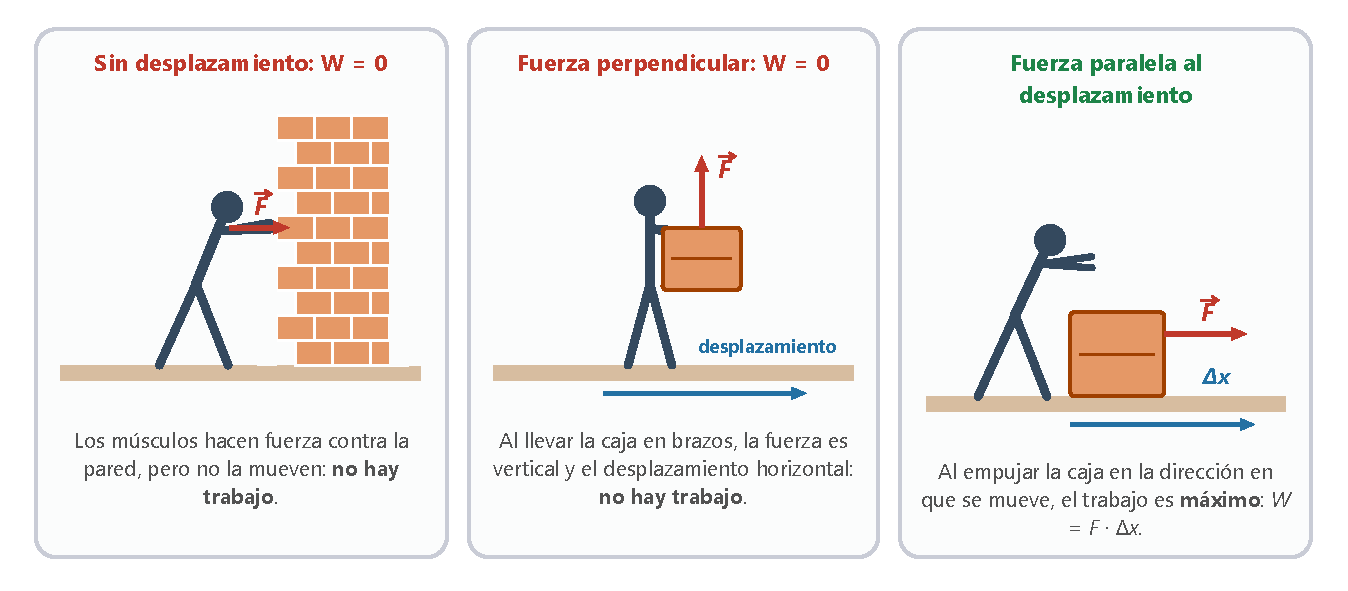
\includegraphics[width=\textwidth]{images/UD12/trabajo_casos}
    \caption{Solo hay trabajo si la fuerza produce un desplazamiento con una componente en su dirección.}
    \label{fig:ud12-casos}
\end{figure}

\subsection{Trabajo de una fuerza constante}

\begin{definition}[Trabajo mecánico]
    El trabajo que realiza una fuerza constante \(\vec{F}\) cuando su punto de aplicación se desplaza \(\Delta\vec{r}\) es el producto
    escalar de ambos vectores:
    \[ W = \vec{F} \cdot \Delta\vec{r} = F\,\Delta r\cos\alpha \]
    donde \(\alpha\) es el ángulo que forman la fuerza y el desplazamiento. Su unidad en el SI es el \textbf{julio} (J).
\end{definition}

\begin{itemize}
    \item \(\qty{1}{\joule}\) es el trabajo que hace una fuerza de \qty{1}{\newton} al desplazar su punto de aplicación \qty{1}{\m} en
    su misma dirección y sentido: \(\qty{1}{\joule} = \qty{1}{\newton\m} = \qty{1}{\kg\m\squared\per\s\squared}\).
    \item Es una magnitud \textbf{escalar}: no depende del sistema de coordenadas elegido.
    \item Solo trabaja la \textbf{componente de la fuerza paralela al desplazamiento}, \(F\cos\alpha\) (figura~\ref{fig:ud12-angulo}).
    \item El trabajo no depende del tiempo que se tarde en hacerlo.
\end{itemize}

\begin{remark}
    No hay que confundir \textbf{esfuerzo} con \textbf{trabajo}. Empujar una pared o sostener una maleta cansa mucho, porque los
    músculos consumen energía química, pero la fuerza que hacemos no realiza trabajo sobre la pared ni sobre la maleta, porque no las
    desplaza.
\end{remark}

\begin{figure}[H]
    \centering
    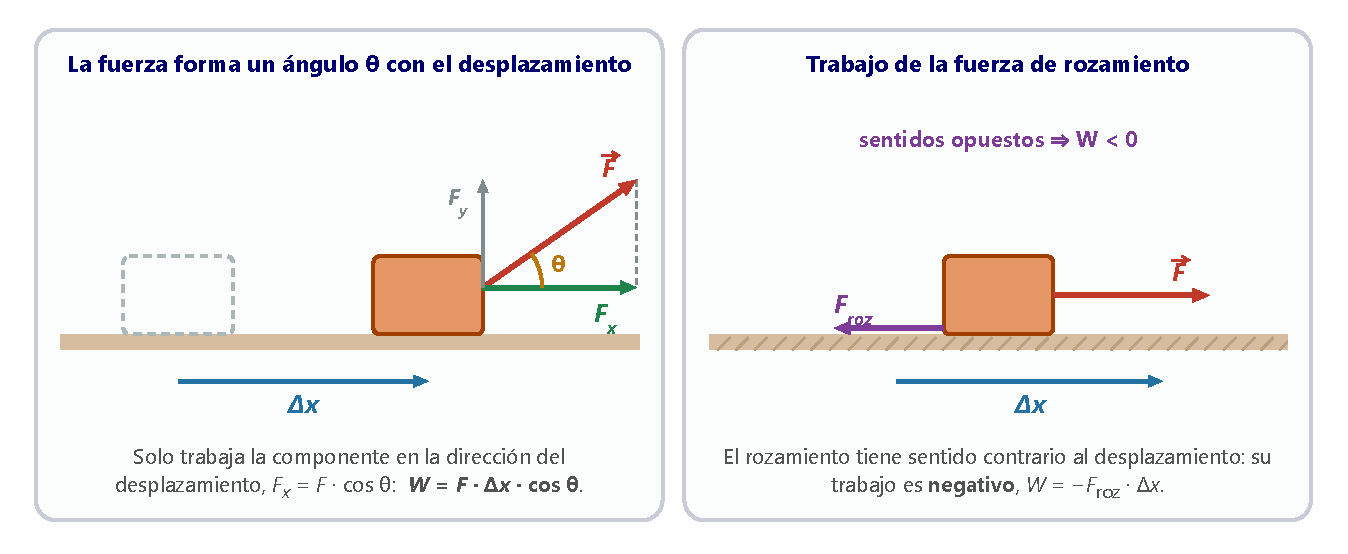
\includegraphics[width=\textwidth]{images/UD12/trabajo_angulo}
    \caption{Trabajo de una fuerza oblicua y de la fuerza de rozamiento.}
    \label{fig:ud12-angulo}
\end{figure}

\begin{example}
    \textbf{¿Hay trabajo?} Calcula el trabajo en estos casos: a) la fuerza con que sostenemos una mochila de \qty{8}{\kg} sin moverla;
    b) la fuerza gravitatoria que la Tierra ejerce sobre un satélite en órbita circular; c) una fuerza horizontal de \qty{10}{\newton}
    que desplaza \qty{60}{\cm} un carrito por un suelo horizontal.

    \textbf{Solución.} a) No hay desplazamiento: \(W = 0\). b) En una órbita circular, la fuerza gravitatoria apunta al centro y es
    siempre perpendicular al desplazamiento: \(W = F\,\Delta r\cos 90^\circ = 0\). c) \(W = 10 \cdot \num{0.6} \cdot \cos 0^\circ = \qty{6}{\joule}\).
\end{example}

\subsection{El signo del trabajo}

El signo del trabajo depende del ángulo entre la fuerza y el desplazamiento:

\begin{table}[H]
    \centering
    \caption{Signo del trabajo según el ángulo \(\alpha\) entre la fuerza y el desplazamiento}
    \vspace{-5pt}
    \begin{tabular}{@{}cL{11cm}@{}}
        \toprule
        \textbf{Ángulo} & \textbf{Trabajo} \\
        \midrule
        \(\alpha = 0^\circ\) & Fuerza y desplazamiento tienen la misma dirección y sentido: el trabajo es \textbf{máximo},
        \(W = F\,\Delta r\). \\[3pt]
        \(0^\circ \leq \alpha < 90^\circ\) & \(\cos\alpha > 0\): trabajo \textbf{positivo} o \textbf{motor}; la fuerza favorece el
        movimiento. \\[3pt]
        \(\alpha = 90^\circ\) & Fuerza perpendicular al desplazamiento: trabajo \textbf{nulo}. \\[3pt]
        \(90^\circ < \alpha \leq 180^\circ\) & \(\cos\alpha < 0\): trabajo \textbf{negativo} o \textbf{resistente}; la fuerza se opone
        al movimiento. \\
        \bottomrule
    \end{tabular}
    \label{tab:ud12-signo}
\end{table}

La \textbf{normal} y la \textbf{fuerza centrípeta} son ejemplos claros de trabajo nulo, porque son perpendiculares a la velocidad. El
\textbf{rozamiento cinético} sobre un cuerpo que desliza por una superficie fija se opone al deslizamiento, así que su trabajo es
negativo: \(W_r = -F_r\,\Delta r\).

\paragraph{Trabajo de varias fuerzas.} Si sobre un cuerpo actúan varias fuerzas, el \textbf{trabajo total} es la suma de los trabajos
de cada una, que coincide con el trabajo de la fuerza resultante:
\[ W_{\text{total}} = W_1 + W_2 + W_3 + \dots = \left(\sum \vec{F}\right) \cdot \Delta\vec{r} = F_{\text{neta}}\,\Delta r\cos\alpha \]

\begin{example}
    \textbf{El trabajo del peso en halterofilia.} Una halterófila levanta una barra de \qty{105}{\kg} hasta \qty{2.1}{\m} de altura.
    Calcula el trabajo que realiza el peso de la barra cuando: a) la barra sube \qty{2.1}{\m}; b) la deja caer y baja \qty{2.1}{\m};
    c) la barra rueda \qty{60}{\cm} por la tarima.

    \textbf{Solución.} \(P = 105 \cdot \num{9.8} = \qty{1029}{\newton}\).

    a) El peso apunta hacia abajo y la barra sube (\(\alpha = 180^\circ\)): \(W = 1029 \cdot \num{2.1} \cdot \cos 180^\circ = \qty{-2161}{\joule}\).
    Es un trabajo resistente.

    b) Peso y desplazamiento van hacia abajo (\(\alpha = 0^\circ\)): \(W = \qty{+2161}{\joule}\), un trabajo motor.

    c) El peso es perpendicular al desplazamiento horizontal: \(W = 0\).
\end{example}

\begin{exercise}
    Sobre una caja que se desliza por el suelo actúa una fuerza de \qty{90}{\newton}. Calcula su trabajo en un recorrido de \qty{12}{\m}
    si: a) tiene la dirección y el sentido del desplazamiento; b) forma \(45^\circ\) con él; c) es vertical hacia arriba; d) forma
    \(150^\circ\) con el desplazamiento.
    \begin{solu}
        a) \(\textcolor{red}{\qty{1080}{\joule}}\). b) \(90 \cdot 12 \cdot \cos 45^\circ = \textcolor{red}{\qty{764}{\joule}}\). c)
        \(\textcolor{red}{0}\). d) \(90 \cdot 12 \cdot \cos 150^\circ = \textcolor{red}{\qty{-935}{\joule}}\).
    \end{solu}
\end{exercise}

\begin{exercise}
    Un niño arrastra \qty{15}{\m} un trineo de \qty{20}{\kg} por un suelo horizontal tirando de una cuerda con una fuerza de
    \qty{60}{\newton} que forma \(30^\circ\) con la horizontal. El coeficiente de rozamiento es \num{0.1}. Calcula el trabajo de cada
    fuerza y el trabajo total.
    \begin{solu}
        \(W_F = 60 \cdot 15 \cdot \cos 30^\circ = \textcolor{red}{\qty{779}{\joule}}\); \(W_P = W_N = \textcolor{red}{0}\).
        \(N = 196 - 60\sen 30^\circ = \qty{166}{\newton}\); \(W_r = -\num{0.1} \cdot 166 \cdot 15 = \textcolor{red}{\qty{-249}{\joule}}\).
        \(W_{\text{total}} = \textcolor{red}{\qty{530}{\joule}}\).
    \end{solu}
\end{exercise}

\subsection{Interpretación gráfica del trabajo}

Si representamos la componente de la fuerza en la dirección del movimiento frente a la posición, el \textbf{trabajo es el área
comprendida entre la gráfica y el eje horizontal} (figura~\ref{fig:ud12-areas}). Esta idea permite calcular el trabajo de fuerzas
variables, como la de un muelle, para las que no sirve la expresión \(W = F\,\Delta x\cos\alpha\).

\begin{figure}[H]
    \centering
    \begin{tikzpicture}
        \begin{axis}[grafica, width=0.36\linewidth, height=4.2cm, xlabel={\(x\)}, ylabel={\(F\)}, xmin=0, xmax=6, ymin=0, ymax=5,
            xtick=\empty, ytick=\empty, title={\small Fuerza constante}]
            \addplot[fill=ocre!25, draw=none] coordinates {(1,0) (1,3) (5,3) (5,0)} \closedcycle;
            \addplot[very thick, ocre, domain=0:6] {3};
            \node[font=\small] at (axis cs:3,1.5) {\(W = F\,\Delta x\)};
        \end{axis}
    \end{tikzpicture}\hfill
    \begin{tikzpicture}
        \begin{axis}[grafica, width=0.36\linewidth, height=4.2cm, xlabel={\(x\)}, ylabel={\(F\)}, xmin=0, xmax=6, ymin=0, ymax=5,
            xtick=\empty, ytick=\empty, title={\small Fuerza elástica}]
            \addplot[fill=ocre!25, draw=none, domain=0:4.5] {0.9*x} \closedcycle;
            \addplot[very thick, ocre, domain=0:5.5] {0.9*x};
            \node[font=\small] at (axis cs:3.2,0.9) {\(W = \tfrac12 k\,x^2\)};
        \end{axis}
    \end{tikzpicture}\hfill
    \begin{tikzpicture}
        \begin{axis}[grafica, width=0.36\linewidth, height=4.2cm, xlabel={\(x\)}, ylabel={\(F\)}, xmin=0, xmax=6, ymin=0, ymax=5,
            xtick=\empty, ytick=\empty, title={\small Fuerza variable}]
            \addplot[fill=ocre!25, draw=none, domain=0.5:5, samples=50] {2+1.5*sin(deg(x-1))} \closedcycle;
            \addplot[very thick, ocre, domain=0:5.6, samples=50] {2+1.5*sin(deg(x-1))};
            \node[font=\small] at (axis cs:2.8,1.2) {\(W\) = área};
        \end{axis}
    \end{tikzpicture}
    \caption{El trabajo es el área bajo la gráfica fuerza-posición.}
    \label{fig:ud12-areas}
\end{figure}

\begin{example}
    \textbf{Una fuerza que deja de empujar.} Sobre un cuerpo actúa una fuerza paralela al desplazamiento que vale \qty{200}{\newton}
    durante los primeros \qty{3}{\m} y después disminuye uniformemente hasta anularse en \(x = \qty{5}{\m}\). ¿Qué trabajo realiza?

    \textbf{Solución.} El área bajo la gráfica es un rectángulo más un triángulo:
    \[ W = 200 \cdot 3 + \frac{1}{2} \cdot 200 \cdot 2 = 600 + 200 = \qty{800}{\joule} \]
\end{example}

\begin{exercise}
    Para estirar un muelle de constante \qty{400}{\newton\per\m} hay que hacer una fuerza \(F = k\,x\). Representa \(F\) frente al
    alargamiento y calcula, a partir de la gráfica, el trabajo necesario para estirarlo \qty{10}{\cm}.
    \begin{solu}
        Es el área de un triángulo de base \qty{0.1}{\m} y altura \(400 \cdot \num{0.1} = \qty{40}{\newton}\):
        \(W = \frac{1}{2} \cdot \num{0.1} \cdot 40 = \textcolor{red}{\qty{2}{\joule}}\).
    \end{solu}
\end{exercise}

%========================================================================================
\section{La energía cinética}\label{sec:ud12-cinetica}
%========================================================================================

Una nave que despega, una montaña rusa que se lanza cuesta abajo o una bola de bolos que derriba los bolos: todo cuerpo en movimiento
puede transformar su entorno. La palabra \textit{cinética} viene del griego \textit{kinetikós}, «que mueve».

\begin{definition}[Energía cinética]
    Es la energía que tiene un cuerpo por estar en movimiento. Para un cuerpo de masa \(m\) que se mueve con velocidad \(v\):
    \[ E_c = \frac{1}{2}\,m\,v^2 \]
\end{definition}

\begin{itemize}
    \item Es una magnitud \textbf{escalar}: depende del módulo de la velocidad, pero no de su dirección ni de su sentido.
    \item \textbf{Nunca es negativa}, porque \(m\) y \(v^2\) son siempre positivos.
    \item Depende del \textbf{cuadrado} de la velocidad: si la velocidad se duplica, la energía cinética se multiplica por cuatro.
    \item Se relaciona con el momento lineal, \(p = m\,v\): multiplicando y dividiendo por \(m\), \(E_c = \dfrac{m^2\,v^2}{2\,m} = \dfrac{p^2}{2\,m}\).
\end{itemize}

\begin{example}
    \textbf{Pruebas de choque.} En unas pruebas de choque se lanza un coche de \qty{1400}{\kg} a \qty{90}{\km\per\hour} y un camión de
    \qty{3600}{\kg} a \qty{15}{\m\per\s}. ¿Cuál tiene más energía cinética?

    \textbf{Solución.} Pasamos la velocidad del coche al SI: \(\qty{90}{\km\per\hour} = \dfrac{90\,000}{3600} = \qty{25}{\m\per\s}\).
    \[ E_{c,\text{coche}} = \frac{1}{2} \cdot 1400 \cdot 25^2 = \qty{4.38e5}{\joule} \qquad
    E_{c,\text{camión}} = \frac{1}{2} \cdot 3600 \cdot 15^2 = \qty{4.05e5}{\joule} \]
    El coche tiene más energía cinética, aunque su masa es mucho menor: la velocidad influye al cuadrado.
\end{example}

\subsection{Teorema de las fuerzas vivas}

El trabajo y la energía cinética se miden en la misma unidad. Veamos qué relación hay entre ellos en un caso sencillo: un cuerpo de
masa \(m\) que se mueve en línea recta empujado por una fuerza neta constante \(F\) en el sentido del movimiento. El trabajo de esa
fuerza es \(W = F\,\Delta x = m\,a\,\Delta x\). En un MRUA, \(v^2 = v_0^2 + 2\,a\,\Delta x\), así que \(a\,\Delta x = \dfrac{v^2 - v_0^2}{2}\):
\[ W = m\,\frac{v^2 - v_0^2}{2} = \frac{1}{2}\,m\,v^2 - \frac{1}{2}\,m\,v_0^2 = E_{c,f} - E_{c,i} \]
Este resultado es general; lo enunció Gaspard-Gustave \textbf{Coriolis} hacia 1829, a partir de las ideas de Galileo y Leibniz.

\begin{definition}[Teorema de las fuerzas vivas o de la energía cinética]
    El trabajo total realizado sobre un cuerpo (el de todas las fuerzas que actúan sobre él) es igual a la variación de su energía
    cinética:
    \[ W_{\text{total}} = \Delta E_c = E_{c,f} - E_{c,i} \]
\end{definition}

\begin{itemize}
    \item Si \(W_{\text{total}} > 0\), la energía cinética \textbf{aumenta}: el cuerpo acelera.
    \item Si \(W_{\text{total}} < 0\), la energía cinética \textbf{disminuye}: el cuerpo frena.
    \item Si \(W_{\text{total}} = 0\), la energía cinética \textbf{no cambia} (por ejemplo, en un MCU).
\end{itemize}

\begin{figure}[H]
    \centering
    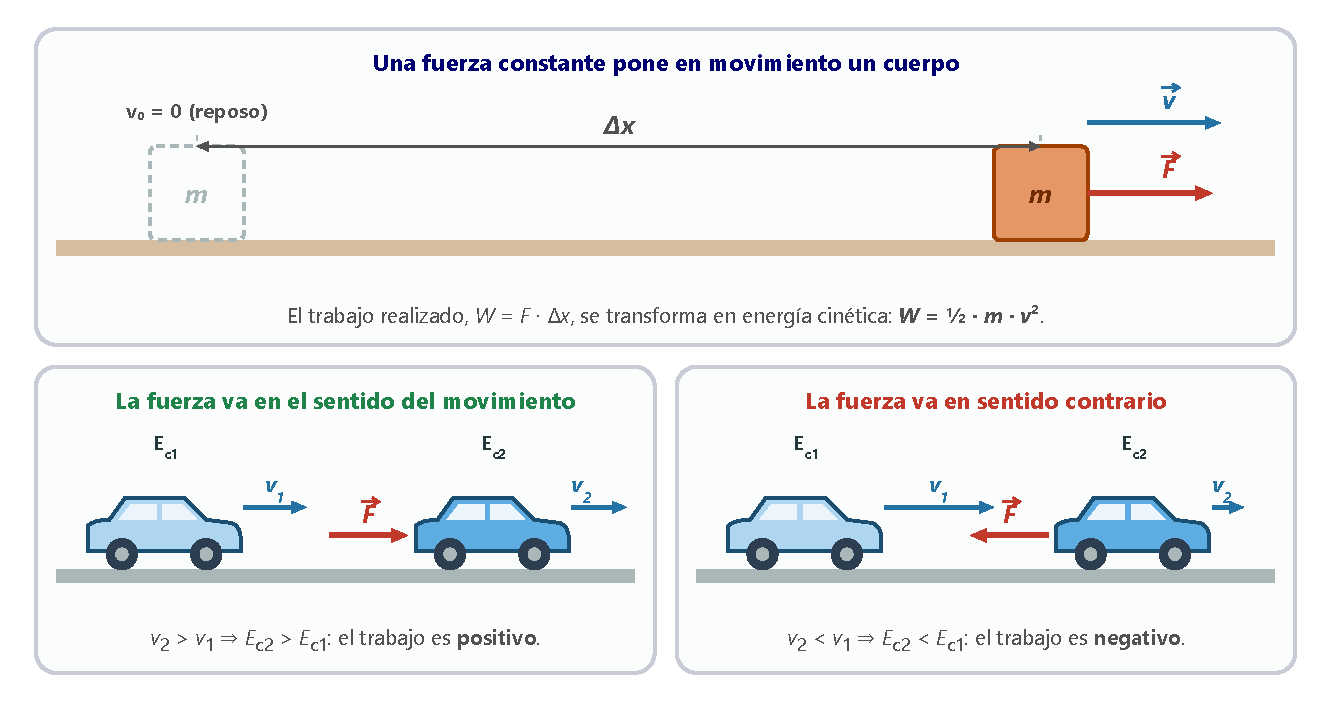
\includegraphics[width=\textwidth]{images/UD12/energia_cinetica}
    \caption{El trabajo de la fuerza neta se invierte en cambiar la energía cinética.}
    \label{fig:ud12-cinetica}
\end{figure}

\begin{remark}
    El trabajo \textbf{no es una forma de energía}, sino una manera de \textbf{transferir} energía de un sistema a otro. Un cuerpo
    tiene energía, pero no «tiene trabajo».
\end{remark}

\begin{example}
    \textbf{Un control de velocidad.} Un coche de \qty{1100}{\kg} circula a \qty{110}{\km\per\hour}, ve un radar y frena hasta
    \qty{80}{\km\per\hour}. ¿Cuánto ha variado su energía cinética? ¿Qué trabajo han hecho los frenos?

    \textbf{Solución.} \(v_i = \qty{30.6}{\m\per\s}\), \(v_f = \qty{22.2}{\m\per\s}\).
    \[ E_{c,i} = \frac{1}{2} \cdot 1100 \cdot \num{30.56}^2 = \qty{5.14e5}{\joule} \qquad E_{c,f} = \frac{1}{2} \cdot 1100 \cdot \num{22.22}^2
    = \qty{2.72e5}{\joule} \]
    \(\Delta E_c = \qty{-2.42e5}{\joule}\). Por el teorema de las fuerzas vivas, el trabajo de los frenos (y demás fuerzas resistentes)
    es \(W = \qty{-2.42e5}{\joule}\); esa energía acaba como calor en los discos de freno.
\end{example}

\begin{example}
    \textbf{Un carro de reparto.} Un repartidor tira de un carro de \qty{18}{\kg}, que parte del reposo, con una fuerza de
    \qty{50}{\newton} que forma \(30^\circ\) con la horizontal, a lo largo de \qty{8}{\m}. Despreciando el rozamiento, calcula: a) el
    trabajo de cada fuerza; b) la velocidad final del carro.

    \textbf{Solución.} a) Sobre el carro actúan el peso, la normal y la fuerza del repartidor. El peso y la normal son perpendiculares al
    desplazamiento: \(W_P = W_N = 0\). Solo trabaja la fuerza aplicada: \(W_F = 50 \cdot 8 \cdot \cos 30^\circ = \qty{346}{\joule}\).

    b) Por el teorema de las fuerzas vivas, \(W_{\text{total}} = \frac{1}{2}\,m\,v^2 - 0\):
    \[ v = \sqrt{\frac{2\,W}{m}} = \sqrt{\frac{2 \cdot 346}{18}} = \qty{6.20}{\m\per\s} \]
\end{example}

\begin{exercise}
    Un velocista de \qty{80}{\kg} alcanza una velocidad máxima de \qty{12}{\m\per\s} en una carrera de \qty{100}{\m}. ¿Qué energía
    cinética tiene en ese momento?
    \begin{solu}
        \(E_c = \frac{1}{2} \cdot 80 \cdot 12^2 = \textcolor{red}{\qty{5760}{\joule}}\).
    \end{solu}
\end{exercise}

\begin{exercise}
    En una partida de \textit{air hockey}, el disco, de \qty{40}{\g}, pasa de \qty{10}{\m\per\s} a \qty{15}{\m\per\s} tras un golpe.
    ¿Qué trabajo ha realizado el mazo sobre el disco?
    \begin{solu}
        \(W = \Delta E_c = \frac{1}{2} \cdot \num{0.04} \cdot (15^2 - 10^2) = \textcolor{red}{\qty{2.5}{\joule}}\).
    \end{solu}
\end{exercise}

\begin{exercise}
    En la salida de una carrera, una moto y su piloto, de \qty{220}{\kg} en total, alcanzan \qty{162}{\km\per\hour} en un tramo de
    \qty{180}{\m}. Calcula la variación de su energía cinética y la fuerza neta media que actúa sobre la moto.
    \begin{solu}
        \(v = \qty{45}{\m\per\s}\): \(\Delta E_c = \frac{1}{2} \cdot 220 \cdot 45^2 = \textcolor{red}{\qty{2.23e5}{\joule}}\);
        \(F = \dfrac{\Delta E_c}{\Delta x} = \textcolor{red}{\qty{1238}{\newton}}\).
    \end{solu}
\end{exercise}

\begin{exercise}
    Un balón de \qty{450}{\g} tiene un momento lineal de \qty{9}{\kg\m\per\s}. Calcula su energía cinética sin calcular antes la
    velocidad. Comprueba el resultado calculando la velocidad.
    \begin{solu}
        \(E_c = \dfrac{p^2}{2\,m} = \dfrac{81}{\num{0.9}} = \textcolor{red}{\qty{90}{\joule}}\); \(v = \dfrac{9}{\num{0.45}} = \qty{20}{\m\per\s}\)
        y \(\frac{1}{2} \cdot \num{0.45} \cdot 20^2 = \qty{90}{\joule}\).
    \end{solu}
\end{exercise}

%========================================================================================
\section{Fuerzas conservativas y energía potencial}\label{sec:ud12-potencial}
%========================================================================================

Una roca en el borde de un acantilado o el muelle comprimido de una lanzadora de paintball no se mueven, pero pueden hacerlo: tienen
energía almacenada por su \textbf{posición} o su \textbf{configuración}. El término \textit{energía potencial} lo introdujo el ingeniero
escocés William Rankine a mediados del siglo \textsc{xix}.

\subsection{Fuerzas conservativas}

\begin{definition}[Fuerza conservativa]
    Una fuerza es conservativa si el trabajo que realiza sobre un cuerpo que pasa de un punto a otro depende solo de las posiciones
    inicial y final, y no del camino seguido. De forma equivalente: su trabajo a lo largo de cualquier trayectoria cerrada es nulo.
\end{definition}

El \textbf{peso} es una fuerza conservativa: tanto si un cuerpo cae en vertical como si baja por un plano inclinado o describe una
parábola, el trabajo del peso es \(m\,g\,h\), donde \(h\) es la diferencia de alturas (figura~\ref{fig:ud12-caminos}). También son
conservativas la \textbf{fuerza elástica} de un muelle, la \textbf{gravitatoria} y la \textbf{electrostática}. El \textbf{rozamiento}, en
cambio, \textbf{no es conservativo}: cuanto más largo es el camino, más trabajo (negativo) realiza. Tampoco lo son, en general, las
fuerzas que aplicamos con las manos o con un motor.

\begin{figure}[H]
    \centering
    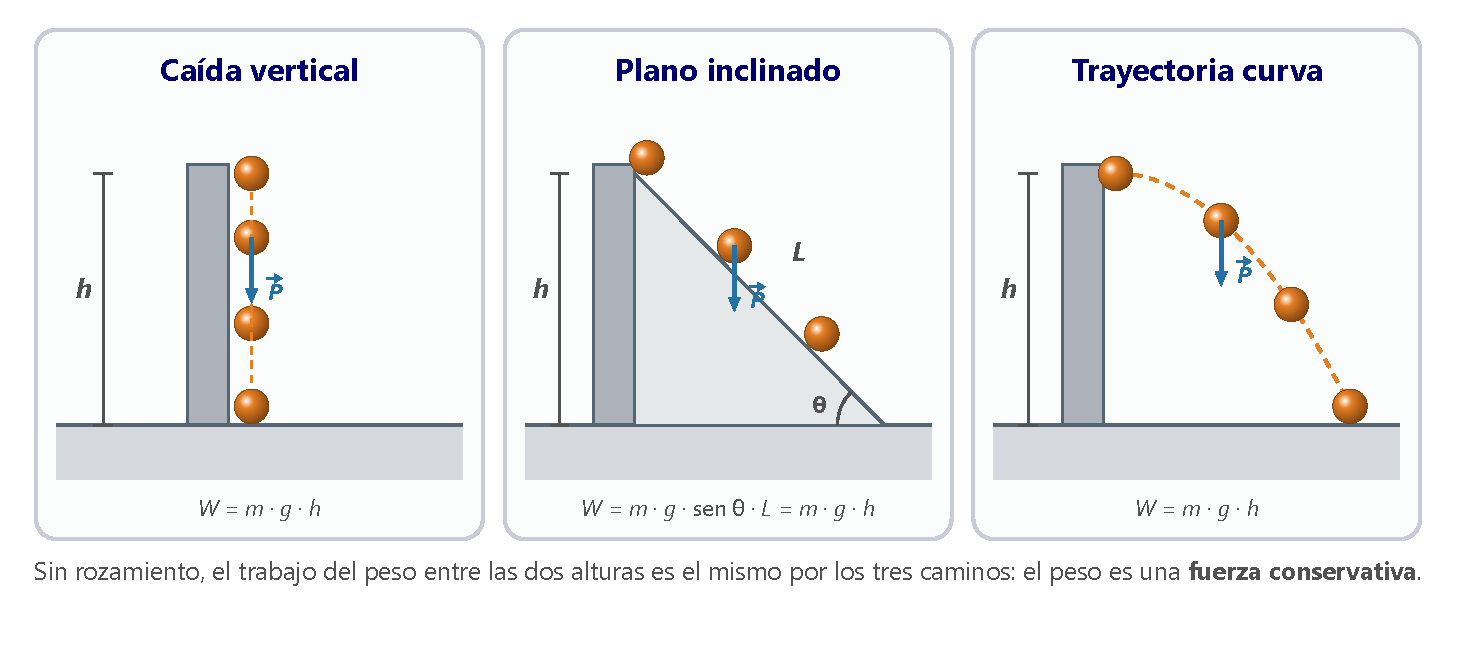
\includegraphics[width=\textwidth]{images/UD12/caminos_peso}
    \caption{El trabajo del peso entre dos alturas no depende del camino.}
    \label{fig:ud12-caminos}
\end{figure}

Como el trabajo de una fuerza conservativa solo depende de los puntos inicial y final, se le puede asociar una función de la posición,
la \textbf{energía potencial}, \(E_p\), de modo que:

\begin{definition}[Energía potencial]
    Es la energía que tiene un cuerpo por su posición o configuración en un campo de fuerzas conservativas. El trabajo de una fuerza
    conservativa es igual a la variación de la energía potencial cambiada de signo:
    \[ W_{\text{cons}} = -\Delta E_p = -(E_{p,f} - E_{p,i}) = E_{p,i} - E_{p,f} \]
\end{definition}

Solo las fuerzas conservativas tienen asociada una energía potencial. Si la fuerza conservativa realiza un trabajo positivo (por
ejemplo, el peso cuando un cuerpo cae), la energía potencial disminuye. Un sistema tiende de forma natural hacia la posición de
\textbf{mínima energía potencial}: una piedra cae, un muelle estirado vuelve a su longitud natural.

\subsection{Energía potencial gravitatoria}

Calculemos el trabajo del peso cuando un cuerpo sube desde una altura \(h_i\) hasta una altura \(h_f\). El peso apunta hacia abajo y
el desplazamiento, hacia arriba:
\[ W_{\text{peso}} = m\,g\,(h_f - h_i)\cos 180^\circ = m\,g\,h_i - m\,g\,h_f \]
Comparando con \(W_{\text{cons}} = E_{p,i} - E_{p,f}\), la energía potencial gravitatoria es:

\begin{definition}[Energía potencial gravitatoria]
    Es la energía que tiene un cuerpo de masa \(m\) situado a una altura \(h\) sobre un nivel de referencia, cerca de la superficie
    terrestre:
    \[ E_p = m\,g\,h \]
\end{definition}

\begin{itemize}
    \item Solo vale para \textbf{alturas pequeñas} comparadas con el radio terrestre, donde \(g\) es constante. Para alturas grandes
    hay que usar la ley de la gravitación universal (lo estudiarás en 2.º de Bachillerato).
    \item Su valor depende del \textbf{nivel de referencia} (\(h = 0\)), que elegimos libremente: puede ser positiva o negativa
    (un cuerpo en el fondo de un pozo tiene \(E_p < 0\) si tomamos como referencia el suelo).
    \item Lo que tiene sentido físico es la \textbf{variación} de energía potencial, que no depende del nivel de referencia.
\end{itemize}

\begin{figure}[H]
    \centering
    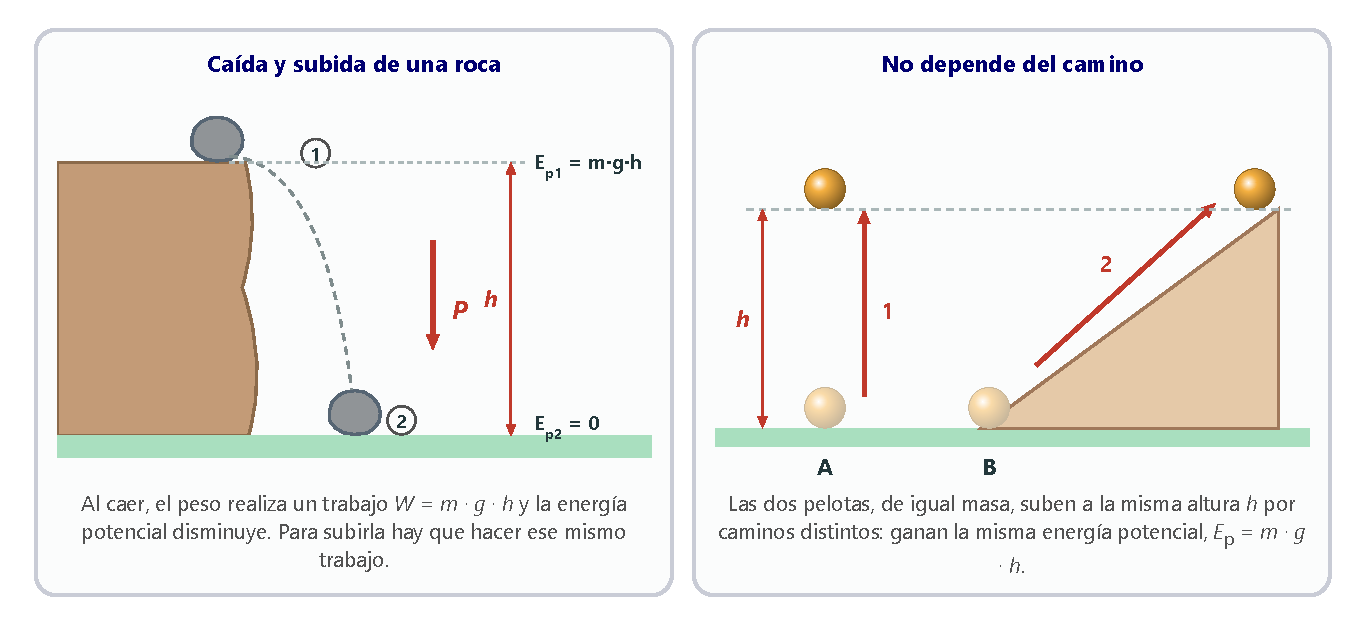
\includegraphics[width=\textwidth]{images/UD12/energia_potencial}
    \caption{La energía potencial gravitatoria depende solo de la altura.}
    \label{fig:ud12-potencial}
\end{figure}

\begin{remark}
    El agua de un embalse tiene energía potencial gravitatoria. En una \textbf{central hidroeléctrica}, el agua cae por unas tuberías
    y mueve las turbinas: su energía potencial se transforma en cinética y después en eléctrica. Es una fuente renovable.
\end{remark}

\begin{example}
    \textbf{Un gato en el balcón.} Un gato de \qty{4}{\kg} está sobre la barandilla de un balcón, a \qty{1}{\m} del suelo del balcón,
    que está a \qty{6}{\m} sobre la calle. a) Calcula su energía potencial respecto al suelo del balcón y respecto a la calle. b) Si salta
    al suelo del balcón, ¿qué trabajo realiza el peso?

    \textbf{Solución.} a) Respecto al balcón: \(E_p = 4 \cdot \num{9.8} \cdot 1 = \qty{39.2}{\joule}\). Respecto a la calle:
    \(E_p = 4 \cdot \num{9.8} \cdot 7 = \qty{274.4}{\joule}\).

    b) \(W = -\Delta E_p\). Con la referencia en el balcón: \(W = -(0 - \num{39.2}) = \qty{39.2}{\joule}\). Con la referencia en la
    calle: \(W = -(4 \cdot \num{9.8} \cdot 6 - \num{274.4}) = \qty{39.2}{\joule}\). El trabajo no depende del nivel de referencia.
\end{example}

\begin{exercise}
    Una persona de \qty{65}{\kg} sube desde la planta baja hasta un cuarto piso; cada planta mide \qty{3}{\m}. ¿Cuánto aumenta su
    energía potencial? ¿Qué trabajo hace el peso?
    \begin{solu}
        \(\Delta E_p = 65 \cdot \num{9.8} \cdot 12 = \textcolor{red}{\qty{7644}{\joule}}\); \(W_{\text{peso}} = \textcolor{red}{\qty{-7644}{\joule}}\).
    \end{solu}
\end{exercise}

\begin{exercise}
    Se deja caer una moneda de \qty{7.5}{\g} desde un mirador situado a \qty{250}{\m} de altura. Despreciando el rozamiento con el
    aire, calcula: a) su energía potencial inicial; b) su energía potencial cuando está a \qty{125}{\m} del suelo; c) su velocidad y su
    energía cinética en ese punto; d) la suma de las energías de b) y c). Explica el resultado.
    \begin{solu}
        a) \(\textcolor{red}{\qty{18.4}{\joule}}\). b) \(\textcolor{red}{\qty{9.19}{\joule}}\). c) \(v = \sqrt{2 \cdot \num{9.8} \cdot 125}
        = \textcolor{red}{\qty{49.5}{\m\per\s}}\); \(E_c = \textcolor{red}{\qty{9.19}{\joule}}\). d) \(\textcolor{red}{\qty{18.4}{\joule}}\):
        la energía potencial perdida se ha convertido en cinética y la suma no cambia. (En realidad, el rozamiento del aire limitaría
        mucho la velocidad).
    \end{solu}
\end{exercise}

\begin{exercise}
    Calcula la energía potencial de una roca de \qty{400}{\kg} en lo alto de un cerro de \qty{120}{\m} respecto a su base.
    \begin{solu}
        \(E_p = 400 \cdot \num{9.8} \cdot 120 = \textcolor{red}{\qty{4.70e5}{\joule}}\).
    \end{solu}
\end{exercise}

\subsection{Energía potencial elástica}

Para estirar o comprimir un muelle hay que aplicar una fuerza igual y opuesta a la recuperadora: según la ley de Hooke,
\(F_{\text{ext}} = k\,x\), donde \(x\) es la deformación respecto a la posición de equilibrio. Como la fuerza crece con la deformación,
el trabajo necesario es el área del triángulo de la gráfica \(F\)-\(x\): \(\frac{1}{2}\,x \cdot k\,x\). Ese trabajo queda
almacenado en el muelle (figura~\ref{fig:ud12-muelle}).

\begin{definition}[Energía potencial elástica]
    Es la energía almacenada en un cuerpo elástico deformado, como un muelle o una goma. Tomando como referencia la posición de
    equilibrio (\(x = 0\)):
    \[ E_{p,\text{elást}} = \frac{1}{2}\,k\,x^2 \]
    donde \(k\) es la constante elástica y \(x\) la deformación (alargamiento o compresión).
\end{definition}

\begin{figure}[H]
    \centering
    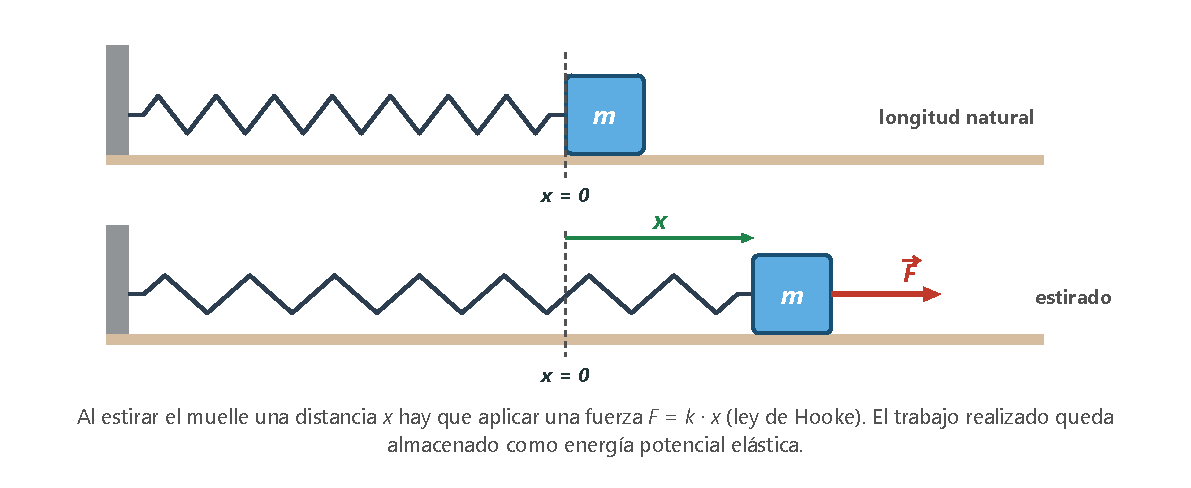
\includegraphics[width=0.85\textwidth]{images/UD12/muelle}
    \caption{Un muelle estirado almacena energía potencial elástica.}
    \label{fig:ud12-muelle}
\end{figure}

\begin{itemize}
    \item Es \textbf{siempre positiva}, tanto si el muelle se estira (\(x > 0\)) como si se comprime (\(x < 0\)), porque depende de
    \(x^2\) (figura~\ref{fig:ud12-parabola}).
    \item El trabajo de la fuerza elástica, que es conservativa, es \(W_{\text{elást}} = -\Delta E_p = \frac{1}{2}\,k\,(x_i^2 - x_f^2)\).
    \item El trabajo de la fuerza exterior que deforma el muelle es igual pero de signo contrario: \(W_{\text{ext}} = \Delta E_p\).
\end{itemize}

\begin{figure}[H]
    \centering
    \begin{tikzpicture}
        \begin{axis}[grafica, width=0.6\linewidth, height=5cm, xlabel={\(x\)}, ylabel={}, xmin=-3, xmax=3, ymin=-3.2, ymax=4.6,
            xtick=\empty, ytick=\empty, axis lines=middle]
            \addplot[very thick, ocre, domain=-2.9:2.9, samples=60] {0.5*x^2};
            \addplot[very thick, blue!60!black, domain=-2.9:2.9] {-x};
            \node[font=\small, ocre] at (axis cs:2.15,4.1) {\(E_p = \tfrac12 k\,x^2\)};
            \node[font=\small, blue!60!black] at (axis cs:2.25,-2.7) {\(F = -k\,x\)};
            \node[font=\scriptsize, align=center] at (axis cs:-1.9,0.4) {compresión};
            \node[font=\scriptsize, align=center] at (axis cs:1.9,0.4) {alargamiento};
        \end{axis}
    \end{tikzpicture}
    \caption{Energía potencial elástica y fuerza recuperadora de un muelle frente a la deformación.}
    \label{fig:ud12-parabola}
\end{figure}

\begin{example}
    \textbf{Una pista de coches de juguete.} En la rampa de lanzamiento de una pista se coloca un coche de \qty{30}{\g} comprimiendo
    \qty{4}{\cm} un muelle de constante \qty{80}{\newton\per\m}. Calcula la energía potencial del muelle y la velocidad con que sale el
    coche si recibe toda esa energía.

    \textbf{Solución.} \(E_p = \frac{1}{2} \cdot 80 \cdot \num{0.04}^2 = \qty{0.064}{\joule}\). Si toda se transforma en energía cinética:
    \[ \frac{1}{2}\,m\,v^2 = E_p \Rightarrow v = \sqrt{\frac{2 \cdot \num{0.064}}{\num{0.03}}} = \qty{2.07}{\m\per\s} \]
\end{example}

\begin{exercise}
    De un muelle de constante \qty{300}{\newton\per\m} se cuelga primero una masa de \qty{2}{\kg} y después otra de \qty{4}{\kg}.
    ¿Cuánto se estira y qué energía potencial elástica almacena en cada caso?
    \begin{solu}
        \(x = \dfrac{m\,g}{k}\): \(\textcolor{red}{\qty{6.5}{\cm}}\) y \(\textcolor{red}{\qty{0.64}{\joule}}\); \(\textcolor{red}{\qty{13.1}{\cm}}\)
        y \(\textcolor{red}{\qty{2.56}{\joule}}\). Al duplicar la masa, la energía se multiplica por cuatro.
    \end{solu}
\end{exercise}

\begin{exercise}
    Al colgar una masa de \qty{600}{\g} de un muelle, este se estira \qty{3}{\cm}. Calcula su constante elástica y la energía que
    almacena.
    \begin{solu}
        \(k = \dfrac{\num{0.6} \cdot \num{9.8}}{\num{0.03}} = \textcolor{red}{\qty{196}{\newton\per\m}}\);
        \(E_p = \frac{1}{2} \cdot 196 \cdot \num{0.03}^2 = \textcolor{red}{\qty{0.088}{\joule}}\).
    \end{solu}
\end{exercise}

\begin{exercise}
    En una caja sorpresa hay dos muñecos, cada uno sobre un muelle de constante \qty{120}{\newton\per\m} comprimido \qty{6}{\cm}. ¿Qué
    energía potencial elástica almacena el conjunto antes de abrir la caja?
    \begin{solu}
        \(E_p = 2 \cdot \frac{1}{2} \cdot 120 \cdot \num{0.06}^2 = \textcolor{red}{\qty{0.43}{\joule}}\).
    \end{solu}
\end{exercise}

\paragraph{Otras formas de energía potencial.} La \textbf{energía química} es energía potencial almacenada en los enlaces entre
átomos: se libera en una combustión y se almacena en la fotosíntesis. La \textbf{energía potencial eléctrica} aparece entre cuerpos
con carga: en una tormenta, un rayo puede liberar del orden de \(10^9\)~J. La \textbf{energía nuclear} es energía potencial asociada a
las fuerzas que mantienen unidos los protones y neutrones del núcleo; se libera en la fisión y en la fusión.

%========================================================================================
\section{Conservación de la energía mecánica}\label{sec:ud12-conservacion}
%========================================================================================

\begin{definition}[Energía mecánica]
    Es la suma de la energía cinética y de todas las formas de energía potencial de un cuerpo:
    \[ E_m = E_c + E_p \]
\end{definition}

Reunamos lo que sabemos: el trabajo total sobre un cuerpo es igual a la variación de su energía cinética, \(W_{\text{total}} = \Delta E_c\),
y el trabajo de las fuerzas conservativas es \(W_{\text{cons}} = -\Delta E_p\).

\subsection{Teorema de conservación de la energía mecánica}

Supongamos que solo realizan trabajo fuerzas conservativas (porque no hay otras o porque, como la normal, no trabajan). Entonces
\(W_{\text{total}} = W_{\text{cons}}\), es decir:
\[ \Delta E_c = -\Delta E_p \Rightarrow E_{c,f} - E_{c,i} = E_{p,i} - E_{p,f} \Rightarrow E_{c,f} + E_{p,f} = E_{c,i} + E_{p,i} \]

\begin{definition}[Teorema de conservación de la energía mecánica]
    Si sobre un sistema solo realizan trabajo fuerzas conservativas, su energía mecánica permanece constante:
    \[ W_{\text{no cons}} = 0 \Rightarrow E_m = E_c + E_p = \text{constante} \]
\end{definition}

La energía mecánica no cambia, pero sus componentes sí: lo que gana la energía cinética lo pierde la potencial, y viceversa
(\(\Delta E_c = -\Delta E_p\)). Es lo que ocurre en un tobogán, en un columpio o en una montaña rusa sin rozamiento
(figura~\ref{fig:ud12-conservacion}).

\begin{figure}[H]
    \centering
    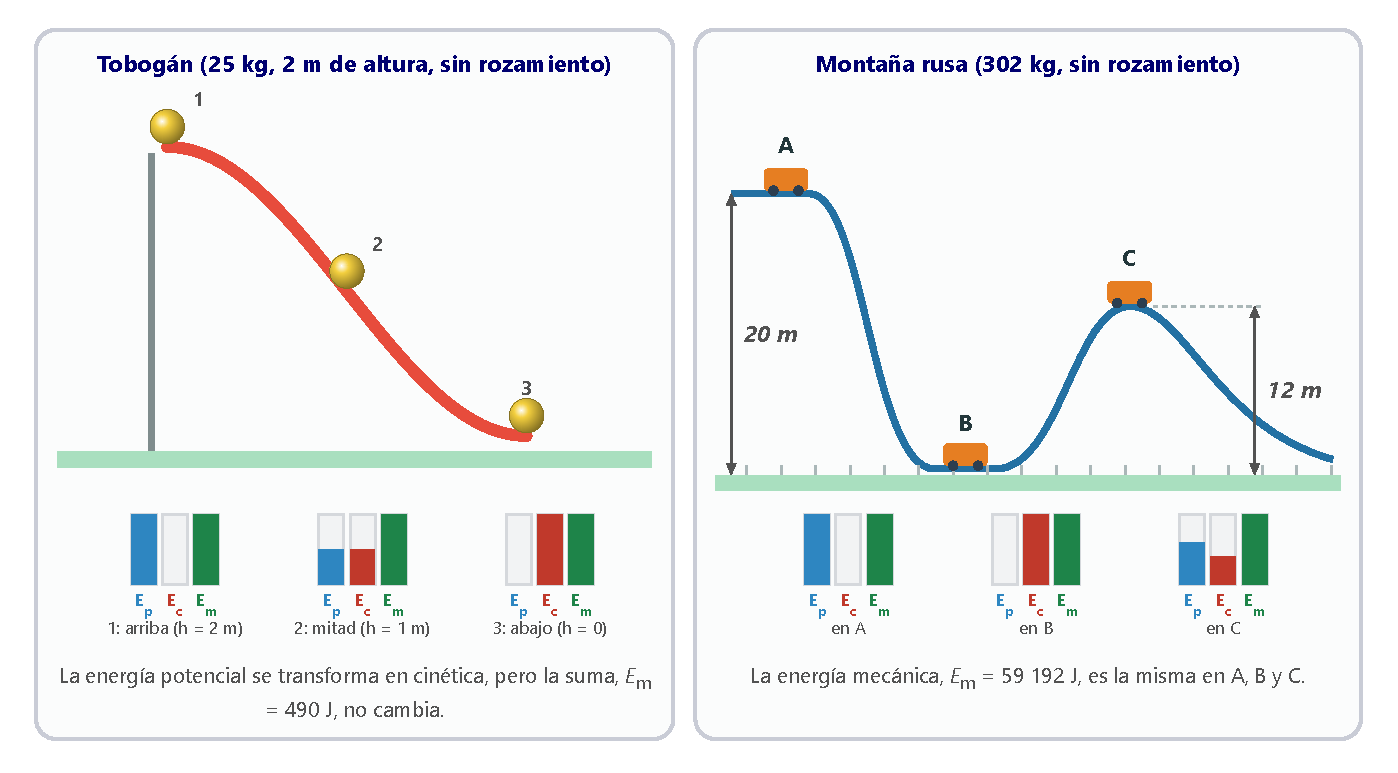
\includegraphics[width=\textwidth]{images/UD12/conservacion}
    \caption{Conservación de la energía mecánica en un tobogán y en una montaña rusa.}
    \label{fig:ud12-conservacion}
\end{figure}

\begin{figure}[H]
    \centering
    \begin{tikzpicture}
        \begin{axis}[grafica, width=0.6\linewidth, height=5cm, xlabel={altura, \(h\)}, ylabel={Energía}, xmin=0, xmax=10.5, ymin=0,
            ymax=12, xtick={0,10}, xticklabels={0,\(h_0\)}, ytick=\empty, legend pos=outer north east, legend style={font=\small}]
            \addplot[very thick, ocre, domain=0:10] {x}; \addlegendentry{\(E_p\)}
            \addplot[very thick, blue!60!black, domain=0:10] {10-x}; \addlegendentry{\(E_c\)}
            \addplot[very thick, dashed, green!50!black, domain=0:10] {10}; \addlegendentry{\(E_m\)}
        \end{axis}
    \end{tikzpicture}
    \caption{Energías de un cuerpo que cae desde una altura \(h_0\) sin rozamiento: la mecánica se mantiene constante.}
    \label{fig:ud12-caida}
\end{figure}

\begin{example}
    \textbf{En el \textit{half-pipe}.} Una patinadora de \qty{55}{\kg} llega al borde de una rampa en U (\textit{half-pipe}) con
    \qty{4}{\m\per\s}. ¿Con qué velocidad pasará por el fondo, \qty{3.5}{\m} más abajo, si no hay rozamiento?

    \textbf{Solución.} Solo trabaja el peso (la normal es perpendicular a la pista): la energía mecánica se conserva. Tomando el fondo
    como referencia:
    \[ \frac{1}{2}\,m\,v_1^2 + m\,g\,h = \frac{1}{2}\,m\,v_2^2 \Rightarrow v_2 = \sqrt{v_1^2 + 2\,g\,h} = \sqrt{16 + 2 \cdot \num{9.8} \cdot \num{3.5}}
    = \qty{9.20}{\m\per\s} \]
    La masa se simplifica: el resultado no depende de ella.
\end{example}

\begin{example}
    \textbf{Caída sobre un muelle.} Desde \qty{60}{\cm} por encima de un muelle vertical de constante \qty{20}{\newton\per\m} se suelta
    un cuerpo de \qty{40}{\g}. ¿Cuánto se comprime el muelle?

    \textbf{Solución.} Tomamos como referencia de alturas el punto de máxima compresión, \(x\) por debajo del extremo del muelle. Al
    principio y al final el cuerpo está en reposo, así que toda la energía potencial gravitatoria se transforma en elástica:
    \[ m\,g\,(\num{0.6} + x) = \frac{1}{2}\,k\,x^2 \Rightarrow \num{0.392} \cdot (\num{0.6} + x) = 10\,x^2 \Rightarrow 10\,x^2 - \num{0.392}\,x - \num{0.235} = 0 \]
    La solución positiva es \(x = \qty{0.174}{\m} = \qty{17.4}{\cm}\).
\end{example}

\begin{exercise}
    Un escalador resbala y cae desde \qty{5}{\m} hasta la colchoneta. ¿Con qué velocidad llega, si despreciamos el rozamiento con el aire?
    \begin{solu}
        \(v = \sqrt{2\,g\,h} = \textcolor{red}{\qty{9.90}{\m\per\s}}\).
    \end{solu}
\end{exercise}

\begin{exercise}
    Una montaña rusa empieza con una gran bajada. ¿Desde qué altura parte, en reposo, el vagón si llega al punto más bajo a
    \qty{30}{\m\per\s}? Desprecia el rozamiento. ¿Influye que el vagón vaya lleno o vacío?
    \begin{solu}
        \(h = \dfrac{v^2}{2\,g} = \textcolor{red}{\qty{45.9}{\m}}\). \textcolor{red}{No influye}: la masa se simplifica.
    \end{solu}
\end{exercise}

\subsection{Fuerzas no conservativas: la energía disipada}

En general, sobre un cuerpo actúan fuerzas conservativas y no conservativas (rozamiento, fuerzas aplicadas, motores):
\[ W_{\text{total}} = W_{\text{cons}} + W_{\text{no cons}} \Rightarrow \Delta E_c = -\Delta E_p + W_{\text{no cons}} \]

\begin{definition}[Trabajo de las fuerzas no conservativas]
    El trabajo de las fuerzas no conservativas es igual a la variación de la energía mecánica:
    \[ W_{\text{no cons}} = \Delta E_m = E_{m,f} - E_{m,i} \]
\end{definition}

\begin{itemize}
    \item Si \(W_{\text{no cons}} > 0\), la energía mecánica \textbf{aumenta} (un motor, una persona que empuja).
    \item Si \(W_{\text{no cons}} < 0\), la energía mecánica \textbf{disminuye}. La energía perdida o \textbf{disipada} se transforma
    en otras formas menos útiles, sobre todo en energía térmica por el rozamiento.
\end{itemize}

La energía total (mecánica más térmica y demás formas) sigue conservándose: el \textbf{principio de conservación de la energía} se cumple
siempre (figura~\ref{fig:ud12-rozamiento}). Lo que ocurre es que la energía se \textbf{degrada}.

\begin{figure}[H]
    \centering
    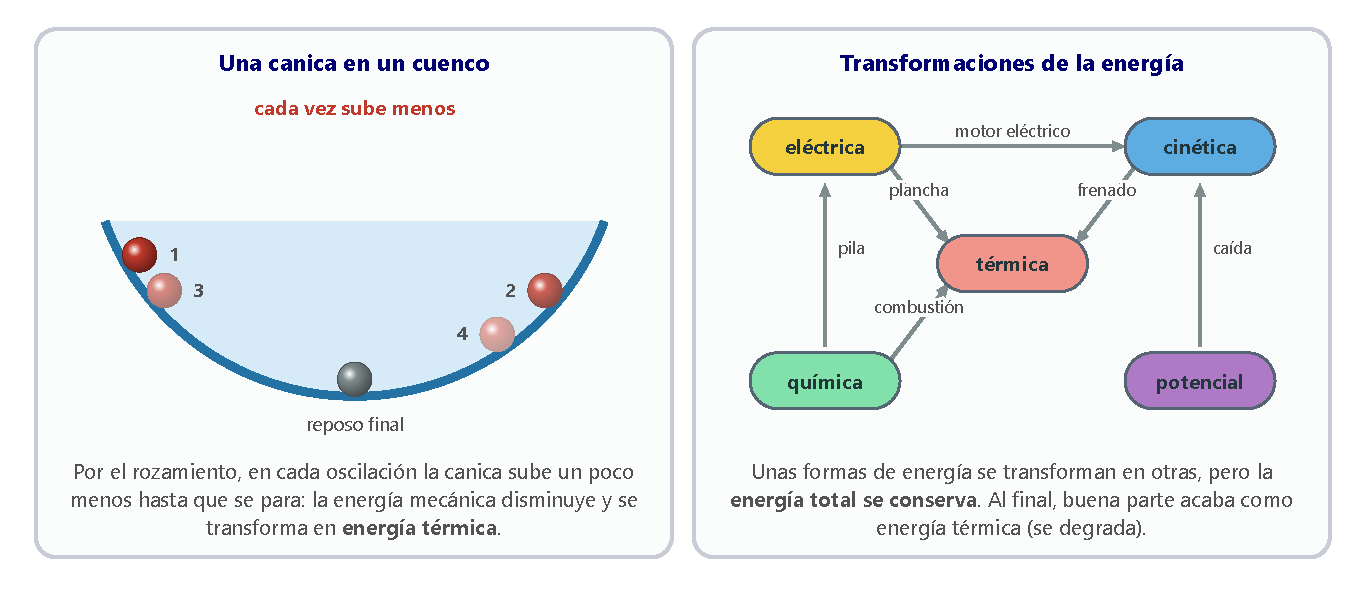
\includegraphics[width=\textwidth]{images/UD12/rozamiento_energia}
    \caption{El rozamiento transforma energía mecánica en térmica; la energía total se conserva.}
    \label{fig:ud12-rozamiento}
\end{figure}

\begin{remark}
    La ecuación de Einstein, \(E = m\,c^2\), muestra que la masa también es una forma de energía. En las reacciones nucleares, una
    pequeña parte de la masa se transforma en una enorme cantidad de energía.
\end{remark}

\begin{example}
    \textbf{El trabajo del motor.} Un coche de \qty{1200}{\kg} arranca y acelera a razón de \qty{2.5}{\m\per\s\squared} durante
    \qty{8}{\s} por una carretera horizontal. Las fuerzas de resistencia (aire y rodadura) equivalen a un coeficiente de rozamiento de
    \num{0.05}. Calcula el trabajo de las fuerzas de resistencia y el del motor.

    \textbf{Solución.} Cinemática: \(x = \frac{1}{2} \cdot \num{2.5} \cdot 8^2 = \qty{80}{\m}\); \(v = \num{2.5} \cdot 8 = \qty{20}{\m\per\s}\).

    Resistencias: \(W_r = -\mu\,m\,g\,x = -\num{0.05} \cdot 1200 \cdot \num{9.8} \cdot 80 = \qty{-4.70e4}{\joule}\).

    La carretera es horizontal, así que la energía mecánica es solo cinética: \(W_{\text{no cons}} = W_{\text{motor}} + W_r = \Delta E_c\):
    \[ W_{\text{motor}} = \frac{1}{2} \cdot 1200 \cdot 20^2 - (\num{-4.70e4}) = \num{2.40e5} + \num{4.70e4} = \qty{2.87e5}{\joule} \]
\end{example}

\begin{exercise}
    Un cuerpo de \qty{12}{\kg} parte del reposo en lo alto de un plano inclinado \(30^\circ\) y de \qty{6}{\m} de longitud. Calcula su
    velocidad al llegar abajo: a) sin rozamiento; b) si actúa una fuerza de rozamiento de \qty{20}{\newton}.
    \begin{solu}
        \(h = 6 \cdot \sen 30^\circ = \qty{3}{\m}\). a) \(v = \sqrt{2\,g\,h} = \textcolor{red}{\qty{7.67}{\m\per\s}}\). b)
        \(W_r = -20 \cdot 6 = \qty{-120}{\joule}\); \(E_c = \num{352.8} - 120 = \qty{232.8}{\joule}\); \(v = \textcolor{red}{\qty{6.23}{\m\per\s}}\).
    \end{solu}
\end{exercise}

\begin{exercise}
    Un esquiador de \qty{80}{\kg} empieza a bajar a \qty{5}{\m\per\s} por una pista de \(20^\circ\) de inclinación y \qty{200}{\m} de
    longitud, con un coeficiente de rozamiento de \num{0.1}. Calcula: a) el trabajo del rozamiento; b) la velocidad al final de la pista.
    \begin{solu}
        a) \(W_r = -\mu\,m\,g\cos 20^\circ \cdot L = \textcolor{red}{\qty{-1.47e4}{\joule}}\). b) \(h = 200\sen 20^\circ = \qty{68.4}{\m}\);
        \(E_{c,f} = 1000 + \num{5.36e4} - \num{1.47e4} = \qty{3.99e4}{\joule}\); \(v = \textcolor{red}{\qty{31.6}{\m\per\s}}\) (en la
        realidad, la resistencia del aire la reduciría bastante).
    \end{solu}
\end{exercise}

%========================================================================================
\section{Potencia y rendimiento}\label{sec:ud12-potencia}
%========================================================================================

Para hacer una mudanza podemos subir las cajas a mano o con un montacargas: el trabajo para elevarlas es el mismo, pero la máquina lo
hace mucho más deprisa. A menudo importa tanto la cantidad de trabajo como la rapidez con que se realiza.

\subsection{Potencia}

\begin{definition}[Potencia media]
    Es el cociente entre el trabajo realizado (o la energía transferida) y el tiempo empleado:
    \[ P = \frac{W}{\Delta t} \]
    Su unidad en el SI es el \textbf{vatio} (W), en honor a James Watt, que perfeccionó la máquina de vapor en 1776:
    \(\qty{1}{\watt} = \qty{1}{\joule\per\s}\).
\end{definition}

\begin{itemize}
    \item Se usan mucho sus múltiplos: \(\qty{1}{\kilo\watt} = \qty{e3}{\watt}\), \(\qty{1}{\mega\watt} = \qty{e6}{\watt}\),
    \(\qty{1}{\giga\watt} = \qty{e9}{\watt}\). En los vehículos se usa todavía el \textbf{caballo de vapor}: \(\text{1 CV} = \qty{735}{\watt}\).
    \item Si una fuerza constante mueve un cuerpo con velocidad media \(v\) en su misma dirección:
    \(P = \dfrac{F\,\Delta x}{\Delta t} = F\,v\). Para una misma potencia, un motor puede dar mucha fuerza a poca velocidad (un tractor)
    o poca fuerza a mucha velocidad (un coche de carreras).
\end{itemize}

\begin{remark}
    El \textbf{kilovatio hora} (kWh) \textbf{no es una unidad de potencia}, sino de energía: es la energía que consume en una hora un
    aparato de \qty{1}{\kilo\watt}. \(\qty{1}{\kilo\watt\hour} = \qty{1000}{\watt} \cdot \qty{3600}{\s} = \qty{3.6e6}{\joule}\). Es la
    unidad que aparece en el recibo de la luz.
\end{remark}

\begin{example}
    \textbf{Trepar por una cuerda.} En una prueba de CrossFit, un atleta de \qty{75}{\kg} sube \qty{4.5}{\m} por una cuerda en
    \qty{6}{\s}. Calcula el trabajo que realiza y su potencia media.

    \textbf{Solución.} El trabajo mínimo que hace es el aumento de su energía potencial:
    \(W = m\,g\,h = 75 \cdot \num{9.8} \cdot \num{4.5} = \qty{3308}{\joule}\). \(P = \dfrac{3308}{6} = \qty{551}{\watt}\), unos
    \num{0.75}~CV.
\end{example}

\begin{exercise}
    Una plataforma elevadora sube una carga de \qty{400}{\kg} a \qty{3}{\m} de altura con velocidad constante de \qty{0.4}{\m\per\s}.
    Calcula la potencia que desarrolla y el trabajo que realiza.
    \begin{solu}
        \(P = F\,v = m\,g\,v = \textcolor{red}{\qty{1568}{\watt}}\); \(W = m\,g\,h = \textcolor{red}{\qty{11760}{\joule}}\) (en \qty{7.5}{\s}).
    \end{solu}
\end{exercise}

\begin{exercise}
    Un horno de \qty{2.2}{\kilo\watt} funciona durante \qty{45}{\minute}. ¿Cuánta energía consume en kWh y en julios? ¿Cuánto cuesta si
    el kWh vale \num{0.15}~€?
    \begin{solu}
        \(E = \num{2.2} \cdot \num{0.75} = \textcolor{red}{\qty{1.65}{\kilo\watt\hour}} = \textcolor{red}{\qty{5.94e6}{\joule}}\); coste:
        \textcolor{red}{\num{0.25}~€}.
    \end{solu}
\end{exercise}

\subsection{Rendimiento}

Las máquinas transforman la energía que reciben en otra más útil: un motor eléctrico transforma energía eléctrica en mecánica, una
batería transforma energía química en eléctrica. Pero ninguna máquina aprovecha toda la energía que recibe: parte se disipa por el
rozamiento entre sus piezas, por efecto Joule, en ruido o en vibraciones (figura~\ref{fig:ud12-rendimiento}):
\[ E_{\text{suministrada}} = W_{\text{útil}} + E_{\text{disipada}} \]

\begin{figure}[H]
    \centering
    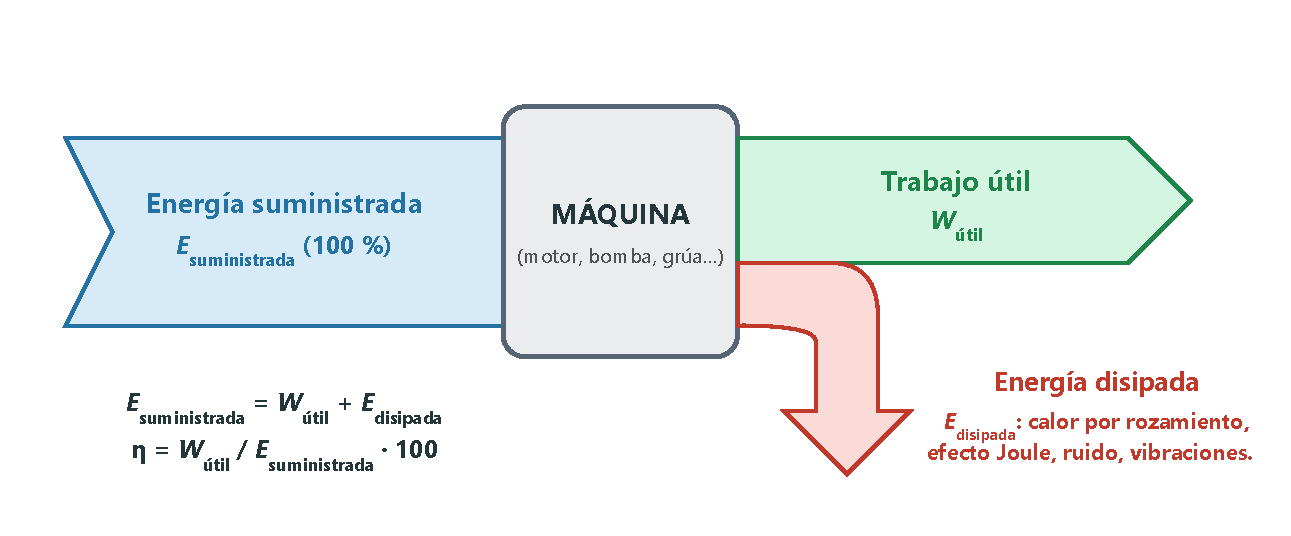
\includegraphics[width=0.8\textwidth]{images/UD12/rendimiento}
    \caption{Balance de energía de una máquina.}
    \label{fig:ud12-rendimiento}
\end{figure}

\begin{definition}[Rendimiento]
    El rendimiento \(\eta\) de una máquina es el cociente, en tanto por ciento, entre el trabajo útil que proporciona y la energía que
    se le suministra (o entre la potencia útil y la potencia consumida):
    \[ \eta = \frac{W_{\text{útil}}}{E_{\text{suministrada}}} \cdot 100 = \frac{P_{\text{útil}}}{P_{\text{consumida}}} \cdot 100 \]
\end{definition}

\begin{itemize}
    \item Siempre es menor que el \qty{100}{\percent}. Lord Kelvin y Max Planck establecieron que es imposible construir una máquina
    térmica que convierta íntegramente en trabajo el calor que recibe (segundo principio de la termodinámica).
    \item Si varias máquinas trabajan en serie, el rendimiento total es el \textbf{producto} de los rendimientos.
    \item Los lubricantes, que reducen el rozamiento, aumentan el rendimiento.
\end{itemize}

\begin{remark}
    \textbf{Rendimiento y eficiencia} no son exactamente lo mismo. La eficiencia es la capacidad de lograr un objetivo con el menor
    consumo de recursos. Una estufa eléctrica tiene un rendimiento cercano al \qty{100}{\percent} (toda la energía eléctrica se
    convierte en calor), pero no sería nada eficiente usarla para enfriar una habitación.
\end{remark}

\begin{example}
    \textbf{Llenar una balsa de riego.} Para regar un olivar se llena una balsa de \qty{500}{\m\cubed} con agua de un pozo de
    \qty{20}{\m} de profundidad. ¿Qué energía hay que suministrar a la bomba si su rendimiento es del \qty{65}{\percent}?
    (\(d_{\text{agua}} = \qty{1000}{\kg\per\m\cubed}\)).

    \textbf{Solución.} El trabajo útil es el aumento de energía potencial del agua:
    \(W_{\text{útil}} = m\,g\,h = 500 \cdot 1000 \cdot \num{9.8} \cdot 20 = \qty{9.8e7}{\joule}\).
    \[ E_{\text{suministrada}} = \frac{W_{\text{útil}}}{\eta} \cdot 100 = \frac{\num{9.8e7}}{65} \cdot 100 = \qty{1.51e8}{\joule} \]
\end{example}

\begin{exercise}
    El motor y los engranajes de la grúa de una obra tienen un rendimiento del \qty{55}{\percent}. ¿Qué energía hay que suministrar
    al motor para subir unas vigas de \qty{800}{\kg} a \qty{20}{\m} de altura?
    \begin{solu}
        \(W_{\text{útil}} = \qty{1.57e5}{\joule}\); \(E = \dfrac{\num{1.57e5}}{\num{0.55}} = \textcolor{red}{\qty{2.85e5}{\joule}}\).
    \end{solu}
\end{exercise}

%========================================================================================
\section{Física en la vida: ITER, un sol en la Tierra}\label{sec:ud12-iter}
%========================================================================================

La humanidad necesita cada vez más energía para mantener su calidad de vida, y las fuentes tradicionales son limitadas o contaminan.
Por eso, científicos de todo el mundo intentan reproducir en la Tierra lo que ocurre en el interior de las estrellas: la \textbf{fusión
nuclear}.

No hay que confundirla con la \textbf{fisión}. En la fisión, un núcleo pesado (normalmente de uranio-235) se rompe en otros más ligeros
al chocar con un neutrón; se liberan energía y nuevos neutrones, que pueden provocar una \textbf{reacción en cadena}. Es lo que ocurre en
las centrales nucleares actuales, que generan residuos radiactivos de larga duración. En la fusión, en cambio, núcleos ligeros (isótopos
del hidrógeno, deuterio y tritio) se unen para formar uno más pesado (helio), como en el Sol. Para que los núcleos, con carga positiva,
venzan su repulsión eléctrica, hay que calentarlos a más de 150 millones de grados.

En una central, la energía nuclear se transforma en energía térmica, que evapora agua; la energía cinética del vapor mueve las
turbinas, y un generador transforma la energía mecánica en eléctrica. La energía se conserva en cada paso, aunque una parte se degrada.

El proyecto internacional \textbf{ITER} (\textit{International Thermonuclear Experimental Reactor}), que se construye en Cadarache
(Francia) con la participación de más de 30 países, pretende demostrar que la fusión es viable. Usa un \textbf{tokamak}, una cámara de
vacío con forma de rosquilla (toroidal) en la que unos potentes imanes mantienen confinado el plasma caliente sin que toque las paredes.
Si se superan los retos técnicos, la fusión sería una fuente casi inagotable de energía, sin emisiones de \ch{CO2} y con muy pocos
residuos: se estima que un gramo de combustible de fusión daría tanta energía como ocho toneladas de petróleo.

\begin{exercise}
    a) Explica la diferencia entre fisión y fusión nuclear. b) El poder calorífico del petróleo es de unos \qty{4.2e7}{\joule\per\kg}.
    ¿Qué energía liberan ocho toneladas de petróleo? ¿Para cuántos hogares bastaría durante un año, si cada uno consume
    \qty{3500}{\kilo\watt\hour} al año? c) Investigad en qué se diferencia el \textit{stellarator}, otro tipo de reactor de fusión, del
    tokamak de ITER.
    \begin{solu}
        a) \textcolor{red}{Fisión}: un núcleo pesado se rompe en otros más ligeros; \textcolor{red}{fusión}: núcleos ligeros se unen
        para formar uno más pesado. b) \(E = 8000 \cdot \num{4.2e7} = \textcolor{red}{\qty{3.4e11}{\joule}} = \qty{9.3e4}{\kilo\watt\hour}\),
        suficiente para unos \textcolor{red}{27 hogares}. c) \textcolor{red}{Respuesta abierta} (el \textit{stellarator} confina el
        plasma solo con imanes de forma retorcida, sin hacer circular corriente por él).
    \end{solu}
\end{exercise}

%========================================================================================
\section{Prácticas}\label{sec:ud12-practicas}
%========================================================================================

\subsection{De energía elástica a energía cinética: un carrete de vasos}

\noindent\begin{minipage}[t]{0.48\textwidth}
    \textbf{Objetivo}
    \begin{itemize}
        \item Comprobar cómo la energía potencial elástica de una goma retorcida se transforma en energía cinética.
    \end{itemize}
\end{minipage}\hfill
\begin{minipage}[t]{0.48\textwidth}
    \textbf{Material}
    \begin{itemize}
        \item Dos vasos de plástico, una pajita, cinta aislante, cuatro gomas elásticas, un clip, un punzón, dos arandelas, tijeras y
        una cinta métrica.
    \end{itemize}
\end{minipage}

\begin{figure}[H]
    \centering
    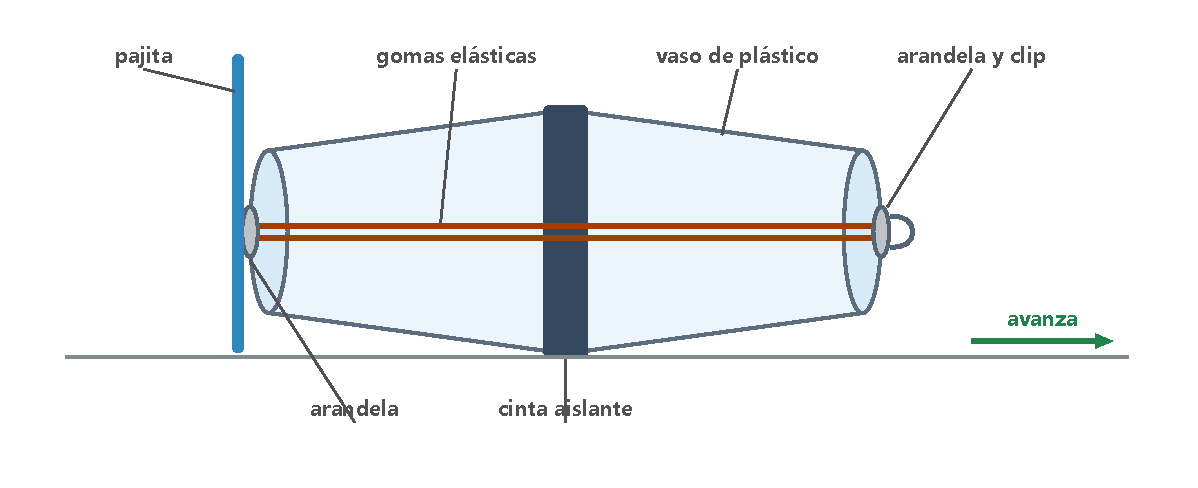
\includegraphics[width=0.75\textwidth]{images/UD12/practica_carrete}
    \caption{Carrete de vasos: al soltarlo, la goma se desenrolla y el carrete avanza.}
    \label{fig:ud12-carrete}
\end{figure}

\textbf{Procedimiento}
\begin{enumerate}[label=\numberballgreen]
    \item Con cuidado, haz un pequeño agujero con el punzón en el centro del fondo de cada vaso.
    \item Une dos gomas para formar una más larga y pásala por el interior de los vasos, sacando un extremo por cada agujero. En un
    extremo, pasa la goma por una arandela y sujétala con el clip; en el otro, pásala por la otra arandela y engánchala a la pajita.
    \item Une las bocas de los vasos con dos vueltas de cinta aislante. La goma debe quedar algo tensa.
    \item Gira la pajita un número de vueltas (10, 20, 30\dots) para retorcer la goma. Apoya el carrete en el suelo sin soltar la
    pajita, suéltala y mide la distancia que recorre. Repite cada medida tres veces.
\end{enumerate}

\begin{exercise}
    a) Describe las transformaciones de energía que se producen desde que giras la pajita hasta que el carrete se para. b) Un grupo
    obtiene estas distancias medias: 10 vueltas, \qty{0.8}{\m}; 20 vueltas, \qty{1.7}{\m}; 30 vueltas, \qty{2.4}{\m}. ¿Qué relación
    observas? c) ¿Por qué acaba parándose el carrete? ¿Se ha perdido la energía?
    \begin{solu}
        a) \textcolor{red}{Química} (de los músculos) \(\rightarrow\) \textcolor{red}{potencial elástica} de la goma \(\rightarrow\)
        \textcolor{red}{cinética} del carrete \(\rightarrow\) \textcolor{red}{térmica} por el rozamiento. b) La distancia es
        \textcolor{red}{aproximadamente proporcional} al número de vueltas: cuanto más se retuerce la goma, más energía almacena.
        c) \textcolor{red}{Por el rozamiento}; la energía no se pierde, se transforma en energía térmica (se degrada).
    \end{solu}
\end{exercise}

\subsection{¿Cuál es nuestra potencia?}

\noindent\begin{minipage}[t]{0.48\textwidth}
    \textbf{Objetivo}
    \begin{itemize}
        \item Calcular la potencia que desarrollamos al subir unas escaleras andando y corriendo.
    \end{itemize}
\end{minipage}\hfill
\begin{minipage}[t]{0.48\textwidth}
    \textbf{Material}
    \begin{itemize}
        \item Un tramo de escaleras, una cinta métrica, un cronómetro (o el móvil) y una báscula.
    \end{itemize}
\end{minipage}

\textbf{Procedimiento}
\begin{enumerate}[label=\numberballgreen]
    \item Mide la altura de un escalón y cuenta los escalones del tramo para calcular la altura total \(h\). Anota tu masa \(m\).
    \item Un compañero cronometra el tiempo que tardas en subir el tramo andando. Repite la medida subiendo deprisa (¡con cuidado!).
    \item Calcula el trabajo que haces contra el peso, \(W = m\,g\,h\), y la potencia, \(P = W/t\), en vatios y en caballos de vapor.
\end{enumerate}

\begin{exercise}
    Una alumna de \qty{60}{\kg} sube 20 escalones de \qty{17}{\cm} en \qty{8.5}{\s} andando y en \qty{3.2}{\s} corriendo. a) Calcula el
    trabajo y la potencia en cada caso. b) ¿Por qué el trabajo es el mismo? c) ¿Es mayor el trabajo realmente hecho por sus músculos?
    \begin{solu}
        a) \(h = \qty{3.4}{\m}\); \(W = \textcolor{red}{\qty{2.0e3}{\joule}}\) en los dos casos; andando, \(P = \textcolor{red}{\qty{235}{\watt}}\);
        corriendo, \(P = \textcolor{red}{\qty{625}{\watt}}\) (\num{0.85}~CV). b) \textcolor{red}{Solo depende de la masa y de la
        altura}, no del tiempo. c) \textcolor{red}{Sí}: el rendimiento de los músculos es bajo (en torno al \qty{25}{\percent}) y gran
        parte de la energía química se transforma en calor.
    \end{solu}
\end{exercise}

%========================================================================================
\section{Situación de aprendizaje: guardar la energía del sol y del viento (ODS 7)}\label{sec:ud12-ods}
%========================================================================================

El \textbf{ODS 7} pide garantizar el acceso a una energía asequible, segura, sostenible y moderna para todos. Desde 2010, más de mil
millones de personas han conseguido electricidad, pero cientos de millones todavía viven sin ella. Al mismo tiempo, para frenar el
cambio climático hay que \textbf{descarbonizar}: sustituir el carbón, el petróleo y el gas por energías renovables. España tiene un
gran potencial solar y eólico, y empresas españolas han sido líderes mundiales en este sector.

Pero el sol y el viento no siempre están disponibles cuando hace falta la energía. Una solución son las \textbf{centrales hidroeléctricas
de bombeo}: cuando sobra electricidad (por ejemplo, a mediodía, con mucha producción solar), se usa para bombear agua desde un embalse
inferior a otro superior; cuando falta, se deja caer el agua y se genera electricidad. Funcionan como una enorme «batería» de energía
potencial gravitatoria. Muy cerca de Almansa, en Cortes de Pallás (Valencia), está el complejo de La Muela, uno de los mayores de Europa,
con un desnivel de unos \qty{500}{\m} entre sus depósitos.

\begin{marker}
    \textbf{Reto:} por grupos, preparad un informe sobre cómo almacenar la energía renovable para que llegue a todos a cualquier hora.
\end{marker}

\begin{enumerate}[label=\numberballred]
    \item \textbf{Investigad} distintas formas de almacenar energía: centrales de bombeo, baterías, hidrógeno verde, sales fundidas en
    centrales termosolares. ¿Qué transformaciones de energía hay en cada una?
    \item \textbf{Calculad} la energía que almacena una central de bombeo (ejercicio siguiente).
    \item \textbf{Analizad} el impacto ambiental de las renovables, con sus ventajas e inconvenientes frente a las no renovables, y qué
    es una vivienda bioclimática.
    \item \textbf{Comunicad} vuestras propuestas para un consumo de energía más sostenible y responsable en vuestro centro.
\end{enumerate}

\begin{exercise}
    El depósito superior de una central de bombeo almacena \qty{2e7}{\m\cubed} de agua con un desnivel de \qty{500}{\m}. a) ¿Qué
    energía potencial almacena, en julios y en kWh? b) Si el rendimiento del ciclo completo (bombear y turbinar) es del \qty{75}{\percent},
    ¿qué energía eléctrica devuelve? c) ¿A cuántos hogares podría abastecer durante un día, si cada uno consume \qty{3500}{\kilo\watt\hour}
    al año?
    \begin{solu}
        a) \(E_p = \num{2e10} \cdot \num{9.8} \cdot 500 = \textcolor{red}{\qty{9.8e13}{\joule}} = \textcolor{red}{\qty{2.7e7}{\kilo\watt\hour}}\)
        (27~GWh). b) \(\textcolor{red}{\qty{2.0e7}{\kilo\watt\hour}}\). c) Cada hogar consume \qty{9.6}{\kilo\watt\hour} al día:
        unos \textcolor{red}{2,1 millones de hogares}.
    \end{solu}
\end{exercise}

    \newpage
    %! Unidad 12 — Energía y trabajo: ejercicios resueltos, ejercicios finales y autoevaluación
%! Fuente: Fuentes/Fisica/Unidad 12 («Ejercicios resueltos», «Practica y calcula», «Piensa y resuelve») y Unidad 13 (captura 452:
%! «Autoevaluación» de este tema; la fuente no trae olimpiadas en este tema). Enunciados adaptados con datos cambiados (y más
%! realistas cuando los de la fuente no lo eran: trepar por una cuerda, potencia de un coche, disco giratorio); soluciones rehechas
%! con g = 9,8 m/s².
%! Dificultad: \(\star\) baja, \(\star\star\) media, \(\star\star\star\) alta.

\section{Ejercicios resueltos}\label{sec:ud12-resueltos}

\begin{example}
    \textbf{El carro de la compra.} Para llevar el carro de la compra, de \qty{22}{\kg}, desde la caja hasta la salida, a \qty{10}{\m},
    tiramos de él con una fuerza de \qty{120}{\newton} que forma \(30^\circ\) con la horizontal. El coeficiente de rozamiento con el
    suelo es \num{0.1}. Calcula el trabajo de cada fuerza y el trabajo total.

    \textbf{Solución.} \textbf{1. Fuerzas}: peso, normal, fuerza aplicada \(F\) (con componentes \(F_x = F\cos 30^\circ\) y
    \(F_y = F\sen 30^\circ\)) y rozamiento. Eje \(X\) en el sentido del movimiento.

    \textbf{2. La normal}: en el eje \(Y\) no hay movimiento: \(N + F_y - P = 0 \Rightarrow N = 22 \cdot \num{9.8} - 120\sen 30^\circ =
    \num{215.6} - 60 = \qty{155.6}{\newton}\); \(F_r = \mu\,N = \qty{15.6}{\newton}\).

    \textbf{3. Trabajo de cada fuerza}:
    \(W_F = 120 \cdot 10 \cdot \cos 30^\circ = \qty{1039}{\joule}\) (solo trabaja \(F_x\));
    \(W_P = W_N = 0\) (perpendiculares al desplazamiento);
    \(W_r = \num{15.6} \cdot 10 \cdot \cos 180^\circ = \qty{-156}{\joule}\).

    \textbf{4. Trabajo total}: \(W_{\text{total}} = 1039 + 0 + 0 - 156 = \qty{883}{\joule}\). Se comprueba que coincide con el trabajo
    de la resultante, que es horizontal: \(W = (F_x - F_r)\,\Delta x = (\num{103.9} - \num{15.6}) \cdot 10 = \qty{883}{\joule}\).
\end{example}

\begin{example}
    \textbf{Una montaña rusa con un looping.} La vagoneta de una montaña rusa, con sus ocupantes, tiene una masa de \qty{750}{\kg}.
    Sube hasta el punto A, a \qty{60}{\m} de altura, y desde allí se deja caer, prácticamente en reposo, hasta el punto más bajo, B,
    donde empieza un looping de \qty{12}{\m} de diámetro (figura~\ref{fig:ud12-looping}). Despreciando el rozamiento, calcula: a) la
    energía mecánica en A; b) la velocidad en B; c) la velocidad en lo alto del looping, C; d) la altura mínima de A para que la vagoneta
    complete el looping.

    \textbf{Solución.} \textbf{1.} Solo trabaja el peso (la normal es perpendicular a la vía): la energía mecánica se conserva. Tomamos
    como referencia de alturas el punto B.

    \textbf{2. a)} En A, \(v = 0\): \(E_m = m\,g\,h_A = 750 \cdot \num{9.8} \cdot 60 = \qty{4.41e5}{\joule}\).

    \textbf{3. b)} En B, \(h = 0\): \(\frac{1}{2}\,m\,v_B^2 = m\,g\,h_A \Rightarrow v_B = \sqrt{2 \cdot \num{9.8} \cdot 60} = \qty{34.3}{\m\per\s}\).

    \textbf{4. c)} En C, \(h_C = \qty{12}{\m}\): \(\frac{1}{2}\,m\,v_C^2 + m\,g\,h_C = m\,g\,h_A \Rightarrow v_C = \sqrt{2\,g\,(h_A - h_C)} =
    \sqrt{2 \cdot \num{9.8} \cdot 48} = \qty{30.7}{\m\per\s}\).

    \textbf{5. d)} En lo alto del looping, la fuerza centrípeta la hacen el peso y la normal (ambos hacia abajo): \(m\,g + N = m\,v_C^2/R\).
    La vagoneta sigue en contacto con la vía si \(N \geq 0\), es decir, si \(v_C^2 \geq g\,R\). Con la conservación de la energía:
    \[ 2\,g\,(h_A - 2R) \geq g\,R \Rightarrow h_A \geq \frac{5}{2}\,R = \num{2.5} \cdot 6 = \qty{15}{\m} \]
\end{example}

\begin{figure}[H]
    \centering
    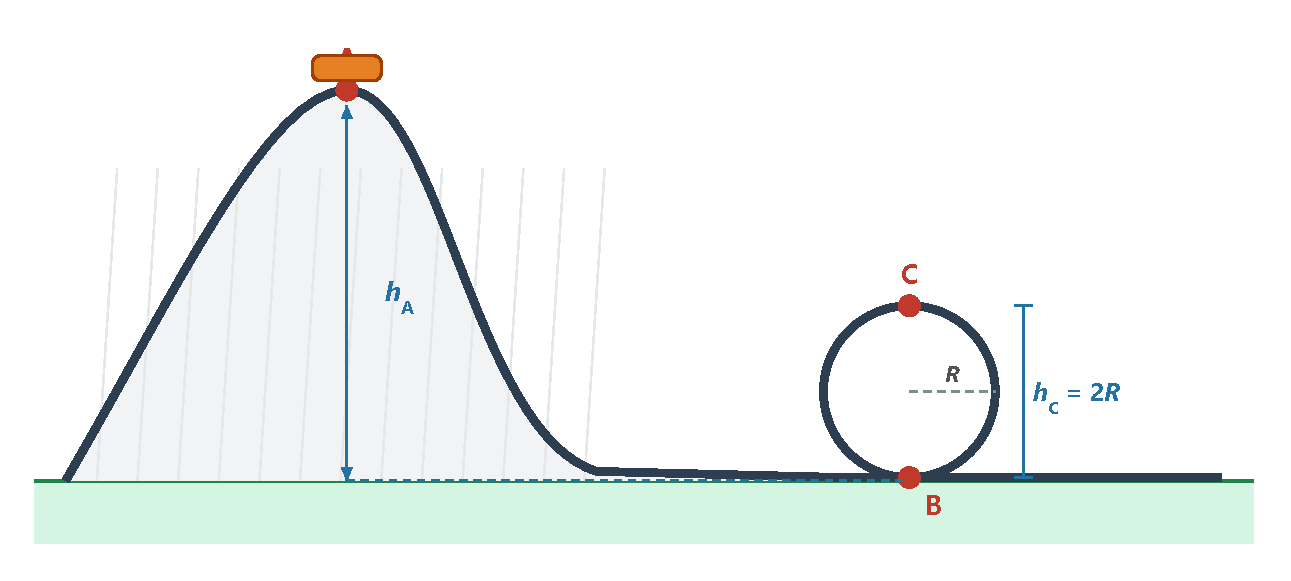
\includegraphics[width=0.75\textwidth]{images/UD12/montana_looping}
    \caption{Montaña rusa con un looping.}
    \label{fig:ud12-looping}
\end{figure}

\begin{example}
    \textbf{Subir y bajar por un plano.} Se lanza un bloque de \qty{3}{\kg} hacia arriba por un plano inclinado \(30^\circ\) con una
    velocidad de \qty{8}{\m\per\s}. El bloque se detiene, vuelve a bajar y llega al punto de partida con \qty{4}{\m\per\s}. Calcula: a) el
    trabajo total del rozamiento; b) la distancia que recorre al subir; c) el coeficiente de rozamiento.

    \textbf{Solución.} \textbf{a)} En el viaje de ida y vuelta, el peso no hace trabajo neto (es conservativo y el cuerpo vuelve al
    mismo punto) y la normal no trabaja. Solo trabaja el rozamiento:
    \(W_r = \Delta E_c = \frac{1}{2} \cdot 3 \cdot (4^2 - 8^2) = \qty{-72}{\joule}\).

    \textbf{b) y c)} Llamamos \(d\) a la distancia recorrida al subir; \(F_r = \mu\,m\,g\cos\alpha\) en los dos tramos.
    \[ \text{Subida: } \frac{1}{2}\,m\,v_0^2 = m\,g\,d\sen\alpha + F_r\,d \qquad \text{Bajada: } m\,g\,d\sen\alpha - F_r\,d = \frac{1}{2}\,m\,v_f^2 \]
    Sumando las dos ecuaciones (y dividiendo entre \(m\)):
    \[ \frac{1}{2}(v_0^2 + v_f^2) = 2\,g\,d\sen\alpha \Rightarrow d = \frac{64 + 16}{4 \cdot \num{9.8} \cdot \num{0.5}} = \qty{4.08}{\m} \]
    Restándolas:
    \[ \frac{1}{2}(v_0^2 - v_f^2) = 2\,\mu\,g\cos\alpha\,d \Rightarrow \mu = \frac{64 - 16}{4 \cdot \num{9.8} \cdot \cos 30^\circ \cdot \num{4.08}} = \num{0.35} \]
\end{example}

\begin{example}
    \textbf{Una lanzadera de coches.} Una pista de juguete tiene un muelle de constante \qty{500}{\newton\per\m}, un tramo horizontal de
    \qty{40}{\cm} y un plano inclinado \(30^\circ\). Se comprime el muelle \qty{6}{\cm} con un coche de \qty{200}{\g} y se suelta. El
    coeficiente de rozamiento es \num{0.15} en toda la pista. Calcula: a) la energía del muelle; b) la velocidad del coche al llegar al
    plano; c) la distancia que sube por el plano.

    \textbf{Solución.} \textbf{a)} \(E_p = \frac{1}{2} \cdot 500 \cdot \num{0.06}^2 = \qty{0.90}{\joule}\).

    \textbf{b)} En el tramo horizontal, \(W_r = -\mu\,m\,g\,d = -\num{0.15} \cdot \num{0.2} \cdot \num{9.8} \cdot \num{0.4} = \qty{-0.118}{\joule}\).
    Con \(W_{\text{no cons}} = \Delta E_m\): \(E_c = \num{0.90} - \num{0.118} = \qty{0.782}{\joule}\), y \(v = \sqrt{\dfrac{2 \cdot \num{0.782}}{\num{0.2}}} = \qty{2.80}{\m\per\s}\).

    \textbf{c)} En el plano, la energía cinética se invierte en subir y en vencer el rozamiento:
    \[ E_c = m\,g\,L\sen 30^\circ + \mu\,m\,g\cos 30^\circ\,L \Rightarrow L = \frac{\num{0.782}}{\num{0.2} \cdot \num{9.8} \cdot (\num{0.5} + \num{0.15} \cdot \num{0.866})}
    = \qty{0.63}{\m} \]
\end{example}

\begin{example}
    \textbf{Un montacargas.} El motor de un montacargas, con un rendimiento del \qty{80}{\percent}, sube una carga de \qty{500}{\kg} con
    una velocidad constante de \qty{1.5}{\m\per\s}. Calcula: a) la potencia útil; b) la potencia que consume el motor, en kW y en CV;
    c) la energía que consume para subir la carga \qty{30}{\m}, en julios y en kWh.

    \textbf{Solución.} \textbf{a)} A velocidad constante, la fuerza del cable iguala al peso: \(P_{\text{útil}} = F\,v = m\,g\,v =
    500 \cdot \num{9.8} \cdot \num{1.5} = \qty{7350}{\watt}\).

    \textbf{b)} \(P_{\text{consumida}} = \dfrac{P_{\text{útil}}}{\eta} \cdot 100 = \dfrac{7350}{80} \cdot 100 = \qty{9188}{\watt} =
    \qty{9.19}{\kilo\watt}\), es decir, \(\dfrac{9188}{735} = \num{12.5}\)~CV.

    \textbf{c)} Tarda \(t = 30/\num{1.5} = \qty{20}{\s}\): \(E = 9188 \cdot 20 = \qty{1.84e5}{\joule} = \qty{0.051}{\kilo\watt\hour}\).
\end{example}

%========================================================================================
\section{Ejercicios de aplicación}\label{sec:ud12-aplicacion}
%========================================================================================

\subsection{La energía: concepto y tipos}

\begin{exercise}
    \(\star\) ¿Qué es la energía? ¿De dónde procede la que usamos en la Tierra?
    \begin{solu}
        \textcolor{red}{Es la capacidad de los sistemas para producir cambios}. Casi toda procede, directa o indirectamente, del
        \textcolor{red}{Sol} (combustibles fósiles, viento, ciclo del agua, biomasa); el resto, de la \textcolor{red}{energía nuclear}
        de los átomos y del \textcolor{red}{calor interno de la Tierra}.
    \end{solu}
\end{exercise}

\begin{exercise}
    \(\star\) La energía nuclear y la química están relacionadas con los átomos. ¿En qué se diferencian?
    \begin{solu}
        La \textcolor{red}{química} está asociada a los \textcolor{red}{enlaces entre átomos} (los electrones) y se libera en las
        reacciones químicas; la \textcolor{red}{nuclear}, a las fuerzas que mantienen unido el \textcolor{red}{núcleo}, y se libera en la
        fisión y en la fusión, en cantidades millones de veces mayores.
    \end{solu}
\end{exercise}

\begin{exercise}
    \(\star\) Cuando una pila deja de funcionar, decimos que «se ha gastado la energía». Si la energía se conserva, ¿es correcta esta
    afirmación?
    \begin{solu}
        \textcolor{red}{No del todo}: la energía química de la pila no ha desaparecido, se ha transformado en otras formas (eléctrica,
        luminosa, térmica\dots) que ya no podemos aprovechar. La energía se ha \textcolor{red}{degradado}.
    \end{solu}
\end{exercise}

\begin{exercise}
    \(\star\) Indica qué forma de energía interviene en cada caso: a) un muelle comprimido; b) una pila de combustible de hidrógeno;
    c) una bombona de butano; d) las señales de los satélites GPS; e) las aspas de un aerogenerador; f) una noria en movimiento;
    g) la radioterapia; h) un secador de pelo; i) un arco a punto de disparar; j) los protones del acelerador del CERN.
    \begin{solu}
        a) \textcolor{red}{Potencial elástica}. b) \textcolor{red}{Química} (que da eléctrica). c) \textcolor{red}{Química}.
        d) \textcolor{red}{Electromagnética}. e) \textcolor{red}{Cinética}. f) \textcolor{red}{Mecánica} (cinética y potencial).
        g) \textcolor{red}{Electromagnética} o \textcolor{red}{nuclear}. h) \textcolor{red}{Eléctrica}, que se transforma en térmica y
        cinética. i) \textcolor{red}{Potencial elástica}. j) \textcolor{red}{Cinética}.
    \end{solu}
\end{exercise}

\begin{exercise}
    \(\star\) Define con tus palabras qué son las fuentes de energía renovables y no renovables, y clasifica estas: a) combustibles
    fósiles; b) biomasa; c) sol, agua y viento; d) uranio; e) geotérmica.
    \begin{solu}
        \textcolor{red}{Renovables}: b), c) y e). \textcolor{red}{No renovables}: a) y d).
    \end{solu}
\end{exercise}

\begin{exercise}
    \(\star\star\) Busca información sobre las aportaciones de Leibniz, Mayer y Joule al concepto de energía y escribe un breve informe.
    \begin{solu}
        \textcolor{red}{Respuesta abierta}. Leibniz: la \textit{vis viva} (\(m\,v^2\)) que se conserva en los choques; Mayer: primera
        formulación del principio de conservación de la energía; Joule: equivalente mecánico del calor.
    \end{solu}
\end{exercise}

\subsection{El trabajo}

\begin{exercise}
    \(\star\) ¿Es lo mismo trabajo que esfuerzo? Indica si hay trabajo en estas actividades: a) poner un plato en la mesa; b) empujar un
    armario que no se mueve; c) llevar la compra a casa por la calle, sin subir ni bajar; d) hacer una plancha de yoga sin moverse.
    \begin{solu}
        \textcolor{red}{No}. a) \textcolor{red}{Sí} (se levanta el plato). b) \textcolor{red}{No}. c) La fuerza vertical que sostiene la
        bolsa \textcolor{red}{no trabaja} (es perpendicular al desplazamiento). d) \textcolor{red}{No}.
    \end{solu}
\end{exercise}

\begin{exercise}
    \(\star\star\) La fuerza que actúa sobre un cuerpo, paralela al desplazamiento, crece uniformemente desde 0 hasta \qty{40}{\newton}
    en los primeros \qty{2}{\m} y se mantiene en \qty{40}{\newton} hasta \(x = \qty{5}{\m}\). Dibuja la gráfica \(F\)-\(x\) y calcula el
    trabajo.
    \begin{solu}
        Área de un triángulo más un rectángulo: \(W = \frac{1}{2} \cdot 2 \cdot 40 + 3 \cdot 40 = \textcolor{red}{\qty{160}{\joule}}\).
    \end{solu}
\end{exercise}

\begin{exercise}
    \(\star\star\) ¿Hay alguna fuerza que realice trabajo sobre un cuerpo con movimiento circular uniforme? Justifícalo.
    \begin{solu}
        \textcolor{red}{No}: la fuerza neta es centrípeta, perpendicular a la velocidad, y su trabajo es nulo; de hecho, la energía
        cinética no cambia.
    \end{solu}
\end{exercise}

\begin{exercise}
    \(\star\star\) ¿El trabajo de la fuerza de rozamiento es siempre negativo?
    \begin{solu}
        \textcolor{red}{No siempre}. El rozamiento cinético sobre un cuerpo que desliza sobre una superficie fija sí realiza trabajo
        negativo, pero el rozamiento estático puede hacer \textcolor{red}{trabajo positivo}: el que la plataforma de un camión que acelera
        hace sobre una caja que no desliza, o el de una cinta transportadora sobre las maletas.
    \end{solu}
\end{exercise}

\begin{exercise}
    \(\star\star\) Calcula el trabajo en estas situaciones: a) la fuerza que hacemos para sostener sobre los hombros, sin movernos, a una
    persona de \qty{60}{\kg}; b) una fuerza horizontal de \qty{15}{\newton} que desplaza \qty{1.2}{\m} un cuerpo de \qty{30}{\kg} por un
    suelo sin rozamiento; c) la fuerza gravitatoria de la Tierra sobre la Luna, supuesta su órbita circular.
    \begin{solu}
        a) \(\textcolor{red}{0}\). b) \(\textcolor{red}{\qty{18}{\joule}}\). c) \(\textcolor{red}{0}\).
    \end{solu}
\end{exercise}

\begin{exercise}
    \(\star\) Una grúa portuaria levanta un contenedor de \qty{12}{t} a \qty{15}{\m} de altura. ¿Qué trabajo realiza?
    \begin{solu}
        \(W = m\,g\,h = 12\,000 \cdot \num{9.8} \cdot 15 = \textcolor{red}{\qty{1.76e6}{\joule}}\).
    \end{solu}
\end{exercise}

\begin{exercise}
    \(\star\star\) Sobre un cuerpo de \qty{15}{\kg}, que se desplaza \qty{50}{\m} por un plano horizontal, actúa una fuerza de
    \qty{80}{\newton}. Calcula su trabajo si: a) forma \(40^\circ\) con la horizontal; b) es perpendicular al desplazamiento; c) tiene la
    dirección y el sentido del movimiento; d) forma \(135^\circ\) con el desplazamiento.
    \begin{solu}
        a) \(\textcolor{red}{\qty{3.06e3}{\joule}}\). b) \(\textcolor{red}{0}\). c) \(\textcolor{red}{\qty{4.00e3}{\joule}}\).
        d) \(\textcolor{red}{\qty{-2.83e3}{\joule}}\).
    \end{solu}
\end{exercise}

\begin{exercise}
    \(\star\star\) Un cuerpo de \qty{25}{\kg} baja \qty{2}{\m} deslizando por un plano inclinado \(30^\circ\), con un coeficiente de
    rozamiento de \num{0.25}. ¿Qué trabajo total recibe?
    \begin{solu}
        \(W_P = 25 \cdot \num{9.8} \cdot 2 \cdot \sen 30^\circ = \qty{245}{\joule}\); \(W_r = -\num{0.25} \cdot 25 \cdot \num{9.8} \cdot \cos 30^\circ
        \cdot 2 = \qty{-106}{\joule}\); \(W_{\text{total}} = \textcolor{red}{\qty{139}{\joule}}\).
    \end{solu}
\end{exercise}

\begin{exercise}
    \(\star\star\) Una bomba sube agua a un depósito de \qty{300}{\liter} situado en la azotea de un edificio de \qty{60}{\m} de altura.
    ¿Qué trabajo realiza la bomba como mínimo?
    \begin{solu}
        \(W = 300 \cdot \num{9.8} \cdot 60 = \textcolor{red}{\qty{1.76e5}{\joule}}\).
    \end{solu}
\end{exercise}

\subsection{La energía cinética}

\begin{exercise}
    \(\star\) ¿La energía cinética puede ser negativa? ¿Y su variación?
    \begin{solu}
        La energía cinética \textcolor{red}{nunca es negativa}, porque \(m\) y \(v^2\) son positivos. Su \textcolor{red}{variación sí
        puede ser negativa}, cuando el cuerpo frena.
    \end{solu}
\end{exercise}

\begin{exercise}
    \(\star\) ¿De qué depende la energía cinética de un cuerpo? ¿Cómo cambia si se duplica su masa? ¿Y si se duplica su velocidad?
    \begin{solu}
        De la \textcolor{red}{masa y de la velocidad}. Si se duplica la masa, \textcolor{red}{se duplica}; si se duplica la velocidad,
        \textcolor{red}{se multiplica por cuatro}.
    \end{solu}
\end{exercise}

\begin{exercise}
    \(\star\) Explica con tus palabras el teorema de las fuerzas vivas y pon un ejemplo.
    \begin{solu}
        \textcolor{red}{El trabajo de todas las fuerzas que actúan sobre un cuerpo es igual a la variación de su energía cinética}. Por
        ejemplo, al frenar una bici, el trabajo negativo del rozamiento de los frenos disminuye su energía cinética.
    \end{solu}
\end{exercise}

\begin{exercise}
    \(\star\star\) ¿Qué tiene más energía cinética, una moto de \qty{180}{\kg} a \qty{120}{\km\per\hour} o un coche eléctrico de
    \qty{1700}{\kg} a \qty{50}{\km\per\hour}?
    \begin{solu}
        Moto: \(\textcolor{red}{\qty{1.00e5}{\joule}}\); coche: \(\textcolor{red}{\qty{1.64e5}{\joule}}\). \textcolor{red}{El coche}.
    \end{solu}
\end{exercise}

\begin{exercise}
    \(\star\star\) Calcula el trabajo que realiza una ciclista, que con su bicicleta tiene una masa de \qty{85}{\kg}, cuando su velocidad
    aumenta de \qty{30}{\km\per\hour} a \qty{50}{\km\per\hour}. Desprecia el rozamiento.
    \begin{solu}
        \(W = \frac{1}{2} \cdot 85 \cdot (\num{13.89}^2 - \num{8.33}^2) = \textcolor{red}{\qty{5.25e3}{\joule}}\).
    \end{solu}
\end{exercise}

\begin{exercise}
    \(\star\star\) Una roca de \qty{900}{\kg} rueda ladera abajo y llega al pie de la colina con una energía cinética de
    \qty{120000}{\joule}. ¿Con qué velocidad llega?
    \begin{solu}
        \(v = \sqrt{\dfrac{2 \cdot 120\,000}{900}} = \textcolor{red}{\qty{16.3}{\m\per\s}}\).
    \end{solu}
\end{exercise}

\begin{exercise}
    \(\star\star\) Lanzamos una canica de \qty{8}{\g} por el suelo a \qty{2.5}{\m\per\s} y se detiene a los \qty{4}{\m}. ¿Qué fuerza de
    rozamiento ha actuado sobre ella?
    \begin{solu}
        \(F_r\,d = \frac{1}{2}\,m\,v^2 \Rightarrow F_r = \dfrac{\num{0.025}}{4} = \textcolor{red}{\qty{6.3e-3}{\newton}}\).
    \end{solu}
\end{exercise}

\begin{exercise}
    \(\star\star\) Un tren de alta velocidad de \qty{400}{t} circula a \qty{200}{\km\per\hour}. ¿Qué velocidad alcanzará si el trabajo
    neto de las fuerzas que actúan sobre él es de \qty{8.0e8}{\joule}?
    \begin{solu}
        \(E_{c,i} = \qty{6.17e8}{\joule}\); \(E_{c,f} = \qty{1.42e9}{\joule}\); \(v = \textcolor{red}{\qty{84.2}{\m\per\s}} = \qty{303}{\km\per\hour}\).
    \end{solu}
\end{exercise}

\subsection{La energía potencial}

\begin{exercise}
    \(\star\) Un cuerpo está en el fondo de un pozo. ¿Tiene energía potencial gravitatoria?
    \begin{solu}
        Depende del \textcolor{red}{nivel de referencia}. Si lo tomamos en el suelo, su energía potencial es
        \textcolor{red}{negativa}; si lo tomamos en el fondo del pozo, es nula.
    \end{solu}
\end{exercise}

\begin{exercise}
    \(\star\star\) Un cuerpo lleva una velocidad de \qty{72}{\km\per\hour}. ¿A qué altura debería estar para que su energía potencial
    fuera igual a esa energía cinética?
    \begin{solu}
        \(m\,g\,h = \frac{1}{2}\,m\,v^2 \Rightarrow h = \dfrac{20^2}{2 \cdot \num{9.8}} = \textcolor{red}{\qty{20.4}{\m}}\).
    \end{solu}
\end{exercise}

\begin{exercise}
    \(\star\) Si un muelle no está ni comprimido ni estirado, ¿tiene energía potencial elástica?
    \begin{solu}
        \textcolor{red}{No}: \(x = 0\), así que \(E_p = 0\).
    \end{solu}
\end{exercise}

\begin{exercise}
    \(\star\star\) Cuenta la leyenda que Newton pensó en la gravitación al ver caer una manzana. Si la manzana tenía \qty{120}{\g} y
    estaba a \qty{4}{\m} de altura, ¿qué energía potencial tenía?
    \begin{solu}
        \(E_p = \num{0.12} \cdot \num{9.8} \cdot 4 = \textcolor{red}{\qty{4.70}{\joule}}\).
    \end{solu}
\end{exercise}

\begin{exercise}
    \(\star\star\) Dos paracaidistas, con una masa conjunta de \qty{170}{\kg}, saltan en tándem desde lo alto del Burj Khalifa
    (\qty{828}{\m}). Suponiendo que no hubiera rozamiento con el aire, calcula: a) su energía potencial inicial; b) su energía potencial a
    \qty{414}{\m} de altura; c) su velocidad y su energía cinética a esa altura; d) la suma de b) y c). e) ¿Por qué en la realidad la
    velocidad es mucho menor?
    \begin{solu}
        a) \(\textcolor{red}{\qty{1.38e6}{\joule}}\). b) \(\textcolor{red}{\qty{6.90e5}{\joule}}\). c) \(\textcolor{red}{\qty{90.1}{\m\per\s}}\);
        \(\textcolor{red}{\qty{6.90e5}{\joule}}\). d) \(\textcolor{red}{\qty{1.38e6}{\joule}}\): la energía mecánica se conserva.
        e) \textcolor{red}{Por la resistencia del aire}, que limita la velocidad de caída a unos \qty{55}{\m\per\s}.
    \end{solu}
\end{exercise}

\begin{exercise}
    \(\star\star\) Un deportista de \qty{75}{\kg} hace 8 dominadas, subiendo cada vez \qty{0.6}{\m}. Calcula: a) el trabajo que hace
    contra su peso; b) su energía potencial en lo alto de una dominada, respecto a la posición inicial; c) su energía cinética cuando
    corre a \qty{2}{\m\per\s}.
    \begin{solu}
        a) \(W = 8 \cdot 75 \cdot \num{9.8} \cdot \num{0.6} = \textcolor{red}{\qty{3.53e3}{\joule}}\). b) \(\textcolor{red}{\qty{441}{\joule}}\).
        c) \(\textcolor{red}{\qty{150}{\joule}}\).
    \end{solu}
\end{exercise}

\begin{exercise}
    \(\star\star\) Al colgar una masa de \qty{2}{\kg} de un muelle, se estira \qty{5}{\cm}. ¿Cuál es su constante elástica? ¿Qué energía
    potencial elástica almacena?
    \begin{solu}
        \(k = \textcolor{red}{\qty{392}{\newton\per\m}}\); \(E_p = \textcolor{red}{\qty{0.49}{\joule}}\).
    \end{solu}
\end{exercise}

\begin{exercise}
    \(\star\star\) Un resorte de constante \qty{200}{\newton\per\m} mide \qty{40}{\cm}. ¿Qué trabajo hay que hacer para comprimirlo hasta
    que mida \qty{28}{\cm}?
    \begin{solu}
        \(W = \frac{1}{2} \cdot 200 \cdot \num{0.12}^2 = \textcolor{red}{\qty{1.44}{\joule}}\).
    \end{solu}
\end{exercise}

\begin{exercise}
    \(\star\star\) Un halcón peregrino de \qty{1}{\kg} vuela a \qty{60}{\m} de altura y se lanza en picado, desde el reposo, a por una
    presa. Despreciando el rozamiento, calcula: a) su energía potencial inicial; b) su energía potencial a \qty{20}{\m} del suelo; c) su
    velocidad y su energía cinética a esa altura.
    \begin{solu}
        a) \(\textcolor{red}{\qty{588}{\joule}}\). b) \(\textcolor{red}{\qty{196}{\joule}}\). c) \(E_c = \textcolor{red}{\qty{392}{\joule}}\);
        \(v = \textcolor{red}{\qty{28.0}{\m\per\s}}\).
    \end{solu}
\end{exercise}

\subsection{La energía mecánica}

\begin{exercise}
    \(\star\star\) Explica con tus palabras qué es la energía mecánica y en qué condiciones se conserva.
    \begin{solu}
        \textcolor{red}{Es la suma de la energía cinética y la potencial}. \textcolor{red}{Se conserva si solo realizan trabajo fuerzas
        conservativas} (no hay rozamiento ni otras fuerzas que trabajen).
    \end{solu}
\end{exercise}

\begin{exercise}
    \(\star\star\) Un avión de \qty{400}{t} vuela a \qty{900}{\km\per\hour} a \qty{11}{\km} de altura. ¿Cuál es su energía mecánica
    respecto al suelo?
    \begin{solu}
        \(E_c = \qty{1.25e10}{\joule}\); \(E_p = \qty{4.31e10}{\joule}\); \(E_m = \textcolor{red}{\qty{5.56e10}{\joule}}\).
    \end{solu}
\end{exercise}

\begin{exercise}
    \(\star\star\) A una escaladora se le cae la mochila, de \qty{2}{\kg}, desde \qty{25}{\m} de altura. Despreciando el rozamiento,
    calcula: a) la energía potencial de la mochila cuando ha caído \qty{10}{\m}; b) su velocidad a \qty{4}{\m} del suelo.
    \begin{solu}
        a) \(E_p = 2 \cdot \num{9.8} \cdot 15 = \textcolor{red}{\qty{294}{\joule}}\). b) \(v = \sqrt{2 \cdot \num{9.8} \cdot 21} =
        \textcolor{red}{\qty{20.3}{\m\per\s}}\).
    \end{solu}
\end{exercise}

\begin{exercise}
    \(\star\star\) Una gimnasta de trampolín sale hacia arriba con \qty{10}{\m\per\s}. Calcula: a) la altura máxima que alcanza sobre
    el trampolín; b) su velocidad a \qty{3}{\m} de altura; c) a qué altura su velocidad es de \qty{6}{\m\per\s}.
    \begin{solu}
        a) \(h = \dfrac{v^2}{2\,g} = \textcolor{red}{\qty{5.10}{\m}}\). b) \(v = \sqrt{100 - 2 \cdot \num{9.8} \cdot 3} = \textcolor{red}{\qty{6.42}{\m\per\s}}\).
        c) \(h = \dfrac{100 - 36}{2 \cdot \num{9.8}} = \textcolor{red}{\qty{3.27}{\m}}\).
    \end{solu}
\end{exercise}

\begin{exercise}
    \(\star\star\) Un coche teledirigido de \qty{1.2}{\kg} se queda sin batería cuando va a \qty{5}{\m\per\s}, justo al empezar a subir
    una rampa de \(25^\circ\). Si el coeficiente de rozamiento es \num{0.2}, ¿a qué altura se detiene?
    \begin{solu}
        \(\frac{1}{2}\,m\,v^2 = m\,g\,d\,(\sen 25^\circ + \mu\cos 25^\circ) \Rightarrow d = \qty{2.11}{\m}\);
        \(h = d\sen 25^\circ = \textcolor{red}{\qty{0.89}{\m}}\).
    \end{solu}
\end{exercise}

\begin{exercise}
    \(\star\star\) La vagoneta de una montaña rusa, con sus ocupantes, tiene \qty{800}{\kg}. Parte del reposo desde lo alto de la
    primera subida, a \qty{70}{\m}, y baja hasta lo alto de la segunda, a \qty{40}{\m}. Sin rozamiento: a) ¿con qué velocidad pasa por
    la segunda cima? b) ¿Qué trabajo ha hecho el motor para subirla hasta los \qty{70}{\m}?
    \begin{solu}
        a) \(v = \sqrt{2 \cdot \num{9.8} \cdot 30} = \textcolor{red}{\qty{24.2}{\m\per\s}}\). b) \(W = m\,g\,h = \textcolor{red}{\qty{5.49e5}{\joule}}\).
    \end{solu}
\end{exercise}

\begin{exercise}
    \(\star\star\) Una bola de \qty{200}{\g} cuelga de un hilo de \qty{1}{\m}. Se separa hasta que el hilo forma \(60^\circ\) con la
    vertical y se suelta. Calcula su velocidad y la tensión del hilo en el punto más bajo.
    \begin{solu}
        Baja \(h = 1 - \cos 60^\circ = \qty{0.5}{\m}\): \(v = \sqrt{2\,g\,h} = \textcolor{red}{\qty{3.13}{\m\per\s}}\).
        \(T - m\,g = m\,v^2/L \Rightarrow T = \num{1.96} + \num{1.96} = \textcolor{red}{\qty{3.92}{\newton}}\).
    \end{solu}
\end{exercise}

\subsection{Potencia y rendimiento}

\begin{exercise}
    \(\star\) Explica con tus palabras el concepto de potencia y pon ejemplos.
    \begin{solu}
        \textcolor{red}{Es la rapidez con que se realiza un trabajo o se transfiere energía}. Por ejemplo, un ascensor y una persona
        hacen el mismo trabajo al subir una caja, pero el ascensor lo hace en menos tiempo: tiene más potencia.
    \end{solu}
\end{exercise}

\begin{exercise}
    \(\star\star\) ¿Qué potencia desarrolla una grúa que eleva un coche de \qty{1200}{\kg} a \qty{4}{\m} de altura en \qty{12}{\s}?
    Exprésala en kW y en CV.
    \begin{solu}
        \(P = \dfrac{1200 \cdot \num{9.8} \cdot 4}{12} = \textcolor{red}{\qty{3.92}{\kilo\watt}}\) = \textcolor{red}{\num{5.3}~CV}.
    \end{solu}
\end{exercise}

\begin{exercise}
    \(\star\star\) Un coche de carreras de \qty{800}{\kg} pasa de 0 a \qty{100}{\km\per\hour} en \qty{2.6}{\s}. Si el \qty{25}{\percent}
    de la energía que da el motor se pierde por rozamiento, calcula: a) la energía cinética final; b) la potencia media del motor.
    \begin{solu}
        a) \(E_c = \frac{1}{2} \cdot 800 \cdot \num{27.8}^2 = \textcolor{red}{\qty{3.09e5}{\joule}}\). b) El motor aporta
        \(\dfrac{\num{3.09e5}}{\num{0.75}} = \qty{4.12e5}{\joule}\): \(P = \textcolor{red}{\qty{158}{\kilo\watt}}\).
    \end{solu}
\end{exercise}

\begin{exercise}
    \(\star\star\) En una central hidroeléctrica caen \qty{40}{\m\cubed} de agua desde \qty{50}{\m} de altura. Si se aprovecha el
    \qty{85}{\percent} de la energía, ¿cuántas bombillas LED de \qty{10}{\watt} podrían estar encendidas durante una hora?
    \begin{solu}
        \(E = \num{4e4} \cdot \num{9.8} \cdot 50 \cdot \num{0.85} = \qty{1.67e7}{\joule}\); \(n = \dfrac{\num{1.67e7}}{10 \cdot 3600} =
        \textcolor{red}{462~bombillas}\).
    \end{solu}
\end{exercise}

\begin{exercise}
    \(\star\star\) Investiga cómo es la etiqueta energética de los electrodomésticos que se usa en la Unión Europea desde 2021 y qué
    cambió respecto a la anterior.
    \begin{solu}
        \textcolor{red}{Respuesta abierta}: la nueva escala va de la A a la G (desaparecen las clases A+, A++ y A+++), es más exigente,
        indica el consumo en kWh y lleva un código QR con información del producto.
    \end{solu}
\end{exercise}

\begin{exercise}
    \(\star\star\) El motor de una grúa, con sus engranajes, tiene un rendimiento del \qty{60}{\percent}. ¿Qué potencia consume para
    subir unas vigas de \qty{500}{\kg} a \qty{18}{\m} de altura en \qty{1.5}{\minute}?
    \begin{solu}
        \(P_{\text{útil}} = \dfrac{500 \cdot \num{9.8} \cdot 18}{90} = \qty{980}{\watt}\); \(P = \dfrac{980}{\num{0.6}} = \textcolor{red}{\qty{1.63}{\kilo\watt}}\).
    \end{solu}
\end{exercise}

\begin{exercise}
    \(\star\star\) En la azotea de un edificio de \qty{30}{\m} hay un depósito de \qty{250}{\liter}. El motor que sube el agua tiene una
    potencia de \qty{400}{\watt} y tarda \qty{4}{\minute} en llenarlo. ¿Cuál es su rendimiento?
    \begin{solu}
        \(W_{\text{útil}} = 250 \cdot \num{9.8} \cdot 30 = \qty{73500}{\joule}\); \(E = 400 \cdot 240 = \qty{96000}{\joule}\);
        \(\eta = \textcolor{red}{\qty{77}{\percent}}\).
    \end{solu}
\end{exercise}

\begin{exercise}
    \(\star\star\) El frigorífico es el electrodoméstico que más consume en una casa, alrededor del \qty{14}{\percent} del total. La
    etiqueta de uno indica un consumo de \qty{150}{\kilo\watt\hour} al año. Calcula su consumo diario en julios y estima el consumo
    anual del hogar.
    \begin{solu}
        \(\dfrac{150}{365} = \qty{0.411}{\kilo\watt\hour}\) = \(\textcolor{red}{\qty{1.48e6}{\joule}}\) al día; hogar:
        \(\dfrac{150}{\num{0.14}} = \textcolor{red}{\qty{1071}{\kilo\watt\hour}}\) al año.
    \end{solu}
\end{exercise}

%========================================================================================
\section{Ejercicios de ampliación}\label{sec:ud12-ampliacion}
%========================================================================================

\begin{exercise}
    \(\star\star\star\) Una jugadora de voleibol salta para bloquear un remate. ¿De dónde sale la energía que la eleva por encima de la
    red? ¿Qué fuerza la impulsa hacia arriba? ¿Realiza trabajo esa fuerza?
    \begin{solu}
        La energía sale de la \textcolor{red}{energía química de sus músculos}. La fuerza que la impulsa es la
        \textcolor{red}{normal del suelo} (reacción a la fuerza con que sus piernas empujan el suelo), pero
        \textcolor{red}{no realiza trabajo}, porque su punto de aplicación (los pies sobre el suelo) no se desplaza: el trabajo lo
        hacen fuerzas internas de su cuerpo.
    \end{solu}
\end{exercise}

\begin{exercise}
    \(\star\star\star\) Un helicóptero rescata a un senderista de \qty{80}{\kg} elevándolo con un cable que tira de él con una fuerza
    constante de \qty{820}{\newton}. Si parte del reposo, ¿qué velocidad tiene tras subir los \qty{15}{\m} de cable?
    \begin{solu}
        \(W_{\text{total}} = (820 - 80 \cdot \num{9.8}) \cdot 15 = \qty{540}{\joule} = \frac{1}{2}\,m\,v^2 \Rightarrow v = \textcolor{red}{\qty{3.67}{\m\per\s}}\).
    \end{solu}
\end{exercise}

\begin{exercise}
    \(\star\star\star\) El disco de una amoladora, de \qty{12.5}{\cm} de diámetro, gira a \qty{10000}{rpm}. La pieza que se corta ejerce
    sobre el borde del disco una fuerza de rozamiento de \qty{6}{\newton}. ¿Qué potencia debe dar el motor para mantener el giro?
    \begin{solu}
        \(v = \omega\,r = \dfrac{10\,000 \cdot 2\pi}{60} \cdot \num{0.0625} = \qty{65.4}{\m\per\s}\); \(P = F\,v = \textcolor{red}{\qty{393}{\watt}}\).
    \end{solu}
\end{exercise}

\begin{exercise}
    \(\star\star\star\) Un muelle de constante \qty{800}{\newton\per\m}, comprimido \qty{10}{\cm}, lanza un bloque de \qty{500}{\g} por
    una superficie horizontal con un coeficiente de rozamiento de \num{0.2}. ¿Qué distancia recorre el bloque hasta pararse?
    \begin{solu}
        \(\frac{1}{2}\,k\,x^2 = \mu\,m\,g\,d \Rightarrow d = \dfrac{4}{\num{0.2} \cdot \num{0.5} \cdot \num{9.8}} = \textcolor{red}{\qty{4.08}{\m}}\).
    \end{solu}
\end{exercise}

\begin{exercise}
    \(\star\star\star\) En la carrera de camellos de una feria se lanzan bolas hacia arriba por una rampa inclinada \(35^\circ\) para que
    entren en unos agujeros. Una bola lanzada a \qty{7}{\m\per\s} llega justo al último agujero, que está a \qty{2}{\m} de altura. ¿Cuál
    es el coeficiente de rozamiento?
    \begin{solu}
        \(\frac{1}{2}\,v_0^2 = g\,h + \mu\,g\cos 35^\circ \dfrac{h}{\sen 35^\circ} \Rightarrow \num{24.5} = \num{19.6} + \num{27.99}\,\mu
        \Rightarrow \mu = \textcolor{red}{\num{0.18}}\).
    \end{solu}
\end{exercise}

\begin{exercise}
    \(\star\star\star\) Un camión de juguete de \qty{1}{\kg} se suelta desde lo alto de un plano inclinado \(30^\circ\) de \qty{1}{\m}
    de longitud; luego sigue por una pista horizontal y se para tras recorrer \qty{2}{\m}. El coeficiente de rozamiento es el mismo en todo
    el recorrido. Calcula: a) el coeficiente de rozamiento; b) la energía disipada en cada tramo; c) la velocidad al final del plano.
    \begin{solu}
        a) \(m\,g\,L\sen 30^\circ = \mu\,m\,g\,(L\cos 30^\circ + d) \Rightarrow \mu = \dfrac{\num{0.5}}{\num{0.866} + 2} = \textcolor{red}{\num{0.17}}\).
        b) Plano: \(\textcolor{red}{\qty{1.48}{\joule}}\); horizontal: \(\textcolor{red}{\qty{3.42}{\joule}}\) (en total, los
        \qty{4.9}{\joule} de energía potencial inicial). c) \(E_c = \num{4.9} - \num{1.48} = \qty{3.42}{\joule}\); \(v = \textcolor{red}{\qty{2.62}{\m\per\s}}\).
    \end{solu}
\end{exercise}

\begin{exercise}
    \(\star\star\star\) Un cuerpo de \qty{2}{\kg} empieza a bajar con \qty{3}{\m\per\s} por un plano inclinado \(20^\circ\) y de
    \qty{4}{\m} de longitud, sin rozamiento. Al final del plano choca con un muelle de constante \qty{500}{\newton\per\m}. a) ¿Con qué
    velocidad llega al final del plano? b) ¿Cuánto comprime el muelle?
    \begin{solu}
        a) \(v = \sqrt{9 + 2 \cdot \num{9.8} \cdot 4\sen 20^\circ} = \textcolor{red}{\qty{5.98}{\m\per\s}}\).
        b) \(\frac{1}{2}\,m\,v^2 = \frac{1}{2}\,k\,x^2 \Rightarrow x = v\sqrt{m/k} = \textcolor{red}{\qty{0.38}{\m}}\) (suponiendo el
        muelle en la parte horizontal).
    \end{solu}
\end{exercise}

\begin{exercise}
    \(\star\star\star\) Un coche de \qty{1300}{\kg} sube a \qty{90}{\km\per\hour} constantes una carretera con una pendiente del
    \qty{8}{\percent} (sube \qty{8}{\m} por cada \qty{100}{\m} de recorrido horizontal). Las fuerzas de resistencia suman
    \qty{600}{\newton}. a) ¿Qué potencia útil desarrolla el motor? b) Si su rendimiento es del \qty{30}{\percent}, ¿qué potencia obtiene
    del combustible?
    \begin{solu}
        \(\alpha = \arctg \num{0.08}\); \(m\,g\sen\alpha = \qty{1016}{\newton}\). a) \(P = (1016 + 600) \cdot 25 = \textcolor{red}{\qty{40.4}{\kilo\watt}}\).
        b) \(\dfrac{\num{40.4}}{\num{0.3}} = \textcolor{red}{\qty{135}{\kilo\watt}}\).
    \end{solu}
\end{exercise}

\begin{exercise}
    \(\star\star\star\) Una bolita se suelta desde una altura \(h\) por una pista sin rozamiento que termina en un rizo de radio
    \qty{20}{\cm}. a) ¿Cuál es la altura mínima para que la bolita dé la vuelta completa sin despegarse? b) Con esa altura, ¿cuántas veces su
    peso vale la normal en el punto más bajo del rizo?
    \begin{solu}
        a) En lo alto, \(v^2 \geq g\,R\); con la conservación de la energía, \(h \geq \frac{5}{2}\,R = \textcolor{red}{\qty{0.5}{\m}}\).
        b) Abajo, \(v^2 = 2\,g\,h = 5\,g\,R\): \(N = m\,g + m\,v^2/R = \textcolor{red}{6\,m\,g}\), seis veces su peso.
    \end{solu}
\end{exercise}

\begin{exercise}
    \(\star\star\star\) \textbf{Péndulo balístico.} Una bala de \qty{10}{\g} se incrusta en un bloque de madera de \qty{2}{\kg} que
    cuelga de unos hilos, y el conjunto sube \qty{12}{\cm}. a) ¿Con qué velocidad se mueve el conjunto justo después del impacto? b) ¿Qué
    velocidad llevaba la bala? c) ¿Qué porcentaje de la energía cinética de la bala se pierde en el choque?
    \begin{solu}
        a) Después del choque se conserva la energía mecánica: \(V = \sqrt{2 \cdot \num{9.8} \cdot \num{0.12}} = \textcolor{red}{\qty{1.53}{\m\per\s}}\).
        b) En el choque se conserva el momento lineal: \(v = \dfrac{\num{2.01} \cdot \num{1.53}}{\num{0.01}} = \textcolor{red}{\qty{308}{\m\per\s}}\).
        c) \(E_c\) antes: \qty{475}{\joule}; después: \qty{2.36}{\joule}: se pierde el \textcolor{red}{\qty{99.5}{\percent}} (se
        transforma en calor y deformación).
    \end{solu}
\end{exercise}

%========================================================================================
\section{Autoevaluación}\label{sec:ud12-autoevaluacion}
%========================================================================================

\begin{exercise}
    Justifica tus respuestas: a) ¿El trabajo del rozamiento es siempre negativo? b) Si sostienes un cuerpo sin moverlo durante un
    tiempo, ¿realizas trabajo? c) ¿Varía la energía cinética de un cuerpo si solo actúan fuerzas conservativas? d) ¿Puede ser negativa
    la energía potencial gravitatoria?
    \begin{solu}
        a) \textcolor{red}{No siempre} (el rozamiento estático puede hacer trabajo positivo). b) \textcolor{red}{No}: no hay
        desplazamiento. c) \textcolor{red}{Sí puede variar}; lo que se mantiene constante es la energía mecánica. d) \textcolor{red}{Sí},
        si el cuerpo está por debajo del nivel de referencia.
    \end{solu}
\end{exercise}

\begin{exercise}
    Un repartidor arrastra un paquete de \qty{25}{\kg}, inicialmente en reposo, con una fuerza de \qty{100}{\newton} que forma
    \(30^\circ\) con la horizontal. Sin rozamiento, ¿qué velocidad tiene el paquete tras recorrer \qty{4}{\m}?
    \begin{solu}
        \(W = 100 \cdot 4 \cdot \cos 30^\circ = \qty{346}{\joule}\); \(v = \sqrt{\dfrac{2 \cdot 346}{25}} = \textcolor{red}{\qty{5.26}{\m\per\s}}\).
    \end{solu}
\end{exercise}

\begin{exercise}
    Una ciclista que rueda a \qty{40}{\km\per\hour} ve una caída \qty{25}{\m} por delante y frena para no arrollar a los corredores
    caídos. Si la masa del conjunto es de \qty{80}{\kg}, ¿qué fuerza de frenado constante necesita como mínimo?
    \begin{solu}
        \(F\,d = \frac{1}{2}\,m\,v^2 \Rightarrow F = \dfrac{\frac{1}{2} \cdot 80 \cdot \num{11.1}^2}{25} = \textcolor{red}{\qty{198}{\newton}}\).
    \end{solu}
\end{exercise}

\begin{exercise}
    Un cuerpo de \qty{5}{\kg} comprime \qty{6}{\cm} un muelle de constante \qty{900}{\newton\per\m}. Al soltarlo, el muelle lo lanza por una
    superficie horizontal sin rozamiento. ¿Con qué velocidad sale?
    \begin{solu}
        \(v = x\sqrt{k/m} = \num{0.06} \cdot \sqrt{180} = \textcolor{red}{\qty{0.80}{\m\per\s}}\).
    \end{solu}
\end{exercise}

\begin{exercise}
    A una persona que se hace un selfi en una terraza a \qty{40}{\m} de altura se le cae el móvil. Sin rozamiento, calcula: a) la
    velocidad con que llega al suelo; b) su velocidad después de caer \qty{20}{\m}; c) a qué altura sobre el suelo su velocidad es de
    \qty{10}{\m\per\s}.
    \begin{solu}
        a) \(\textcolor{red}{\qty{28.0}{\m\per\s}}\). b) \(\textcolor{red}{\qty{19.8}{\m\per\s}}\). c) \(h = 40 - \dfrac{100}{\num{19.6}} =
        \textcolor{red}{\qty{34.9}{\m}}\).
    \end{solu}
\end{exercise}

\begin{exercise}
    El motor de una grúa eleva una carga de \qty{700}{\kg} a \qty{2}{\m\per\s} constantes. a) ¿Qué potencia útil desarrolla? b) ¿Qué
    potencia consume si su rendimiento es del \qty{70}{\percent}?
    \begin{solu}
        a) \(P = m\,g\,v = \textcolor{red}{\qty{13.7}{\kilo\watt}}\). b) \(\textcolor{red}{\qty{19.6}{\kilo\watt}}\).
    \end{solu}
\end{exercise}

\begin{exercise}
    Una secadora de ropa de \qty{2.5}{\kilo\watt} funciona hora y media. ¿Qué energía consume, en kWh y en julios?
    \begin{solu}
        \(E = \num{2.5} \cdot \num{1.5} = \textcolor{red}{\qty{3.75}{\kilo\watt\hour}} = \textcolor{red}{\qty{1.35e7}{\joule}}\).
    \end{solu}
\end{exercise}


    \chapterimage{images/portada_cabeceras/cabecera_UD13}


    \chapter{Termodinámica}

    %! Unidad 13 — Termodinámica: sistemas, variables y procesos termodinámicos, trabajo y calor, criterio de signos, principio
%! cero y temperatura, propagación del calor, calor específico, calorimetría, cambios de estado, dilatación, trabajo de un gas y
%! diagramas p-V, energía interna y primer principio, entropía, segundo principio y máquinas térmicas (teoría, ejemplos
%! resueltos, ejercicios por apartados, lectura, prácticas y situación de aprendizaje)
%! Fuente: Fuentes/Fisica/Unidad 13 (capturas 452 —portada, mitad derecha— a 463 + solucionario).
%! Texto reescrito; datos de los ejercicios cambiados y recalculados; 1 cal = 4,18 J; R = 8,31 J/(mol·K); 1 atm = 101 325 Pa.
%! Figuras en images/UD13/: nuevas en html/ (principio_cero, escalas_temperatura, mecanismos_calor, cambios_estado,
%!   expansion_embolo, practica_nube), copiadas (PDF + SVG) de 4ESO/images/UD12 (particulas_temperatura, equilibrio_termico,
%!   joule, dilatacion, bimetal, balance_calorimetro, maquina_termica, motor_cuatro_tiempos, practica_calor_especifico) y de
%!   2BachQuimica/FigurasSVG/UD4_Termodinamica (sistemas = UD4_01, energia_interna = UD4_05, criterio_signos = UD4_06).
%!   Gráficas con pgfplots (curva de calentamiento del agua, diagramas p-V).

\section*{Para empezar: subir con aire caliente}
\addcontentsline{toc}{section}{Para empezar: subir con aire caliente}

Al amanecer, sobre los templos de Bagan (Birmania) o sobre los campos de Capadocia (Turquía), decenas de \textbf{globos
aerostáticos} se elevan en silencio. Su funcionamiento es sencillo: un quemador de propano calienta el aire del interior de la
vela; el aire caliente se dilata, se vuelve menos denso que el aire frío que lo rodea y el globo sube. Para bajar basta con dejar
que el aire se enfríe. ¿Qué tiene que ver el calor con el movimiento? ¿Se puede convertir todo el calor del quemador en trabajo
útil?

La \textbf{termodinámica} estudia los intercambios de energía en forma de \textbf{calor} y de \textbf{trabajo}. Está presente en la
física y en la química: en los motores de los coches, en los frigoríficos y las bombas de calor, en las centrales eléctricas, en
las corrientes oceánicas y en fenómenos meteorológicos como las DANA, en las reacciones químicas e incluso en nuestro propio
organismo, que intercambia continuamente materia y energía con el entorno. En esta unidad estudiaremos sus conceptos básicos y sus
tres principios: el \textbf{principio cero} (temperatura y equilibrio térmico), el \textbf{primero} (la conservación de la energía)
y el \textbf{segundo} (la entropía y el sentido de los procesos).

%========================================================================================
\section{Recuerda de la ESO}\label{sec:ud13-eso}
%========================================================================================

\paragraph{Volumen de un cilindro.} Es el área de la base por la altura: \(V = S\,h = \pi\,r^2\,h\). Lo usaremos para el gas
encerrado en un cilindro con un émbolo.

\paragraph{Magnitudes extensivas e intensivas.} Una magnitud es \textbf{extensiva} si su valor depende de la cantidad de materia
(masa, volumen, energía) e \textbf{intensiva} si no depende de ella (temperatura, presión, densidad). Un vaso de agua y una jarra de
agua a la misma temperatura tienen distinto volumen, pero la misma temperatura y la misma densidad.

\paragraph{Teoría cinético-molecular.} La materia está formada por partículas en continuo movimiento desordenado. La
\textbf{temperatura} de un cuerpo es una medida de la \textbf{energía cinética media} de sus partículas.

\paragraph{Presión.} Es la fuerza por unidad de superficie, \(p = F/S\). Su unidad en el SI es el \textbf{pascal} (\(\qty{1}{\pascal}
= \qty{1}{\newton\per\m\squared}\)). También se usan \(\qty{1}{\bar} = \qty{e5}{\pascal}\) y \(\qty{1}{\atm} = \qty{101325}{\pascal} =
\qty{760}{\mmHg}\).

\paragraph{Calor y calor específico.} El \textbf{calor} es energía en tránsito entre dos cuerpos a distinta temperatura; pasa del
más caliente al más frío hasta que se alcanza el \textbf{equilibrio térmico}. Cada sustancia necesita una cantidad distinta de
energía para calentarse: es su \textbf{calor específico}. Para que \qty{1}{\g} de agua suba \qty{1}{\degreeCelsius} hace falta
\qty{1}{\calorie}; para \qty{1}{\g} de hierro basta con \qty{0.11}{\calorie}.

\paragraph{Trabajo.} El trabajo de una fuerza constante es \(W = \vec F \cdot \Delta\vec r = F\,\Delta r\cos\alpha\) y se mide en
julios. Si empujamos el émbolo de una jeringa tapada, hacemos trabajo sobre el gas y le comunicamos energía.

\begin{exercise}
    Un cilindro tiene un radio interior de \qty{4}{\cm} y una altura de \qty{12}{\cm}. a) ¿Qué volumen de gas cabe dentro, en litros?
    b) ¿Qué presión ejerce una fuerza de \qty{50}{\newton} sobre un émbolo que cierra el cilindro?
    \begin{solu}
        a) \(V = \pi \cdot \num{0.04}^2 \cdot \num{0.12} = \qty{6.03e-4}{\m\cubed} = \textcolor{red}{\qty{0.603}{\litre}}\).
        b) \(p = \dfrac{F}{S} = \dfrac{50}{\pi \cdot \num{0.04}^2} = \textcolor{red}{\qty{9.95e3}{\pascal}}\).
    \end{solu}
\end{exercise}

%========================================================================================
\section{Introducción a la termodinámica}\label{sec:ud13-introduccion}
%========================================================================================

El dominio del fuego fue un punto de inflexión para la humanidad: permitió cocinar, calentarse y transformar materiales. Pero la
ciencia del calor no nació hasta el siglo \textsc{xix}, cuando la \textbf{máquina de vapor} obligó a entender cómo convertir calor
en movimiento. En 1824, el ingeniero francés \textbf{Sadi Carnot} estudió el rendimiento de estas máquinas y sentó las bases de la
termodinámica. El nombre procede del griego \textit{thermos} (calor) y \textit{dynamis} (fuerza): reúne la \textbf{termología}, que
estudiaba los fenómenos térmicos, y la \textbf{mecánica}, que estudiaba el movimiento, las fuerzas y el trabajo.

\begin{definition}[Termodinámica]
    Es la parte de la física que estudia los intercambios de energía, en forma de calor y de trabajo, entre un sistema y su
    entorno, y las transformaciones de una forma de energía en otra.
\end{definition}

La termodinámica estudia sistemas \textbf{macroscópicos}, formados por un número enorme de partículas, y se ocupa de sus estados de
\textbf{equilibrio}. Sus principios no se demuestran: son generalizaciones de la \textbf{experiencia} que nunca se han visto
contradichas. La parte de la termodinámica que estudia los intercambios de energía en las reacciones químicas se llama
\textbf{termoquímica} (ya la vimos en la sección~\ref{sec:ud6-energia}).

\subsection{Sistemas termodinámicos}

\begin{definition}[Sistema termodinámico]
    Es la porción del universo que queremos estudiar, separada del resto por una \textbf{pared} o frontera, real o imaginaria. Lo
    que queda fuera y puede intercambiar energía o materia con él es el \textbf{entorno}. Sistema y entorno forman el
    \textbf{universo}.
\end{definition}

Según lo que pueden intercambiar con el entorno, los sistemas son (figura~\ref{fig:ud13-sistemas}):
\begin{itemize}
    \item \textbf{Abiertos}: intercambian materia y energía. Por ejemplo, una cazuela destapada al fuego, una sauna (hay que aportar
    agua y calor) o un ser vivo.
    \item \textbf{Cerrados}: intercambian energía, pero no materia. Un termómetro clínico: su mercurio o su alcohol no salen, pero
    recibe calor del cuerpo.
    \item \textbf{Aislados}: no intercambian ni materia ni energía. Un termo de buena calidad bien cerrado se acerca a este modelo;
    en sentido estricto, el único sistema perfectamente aislado es el universo.
\end{itemize}

\begin{figure}[H]
    \centering
    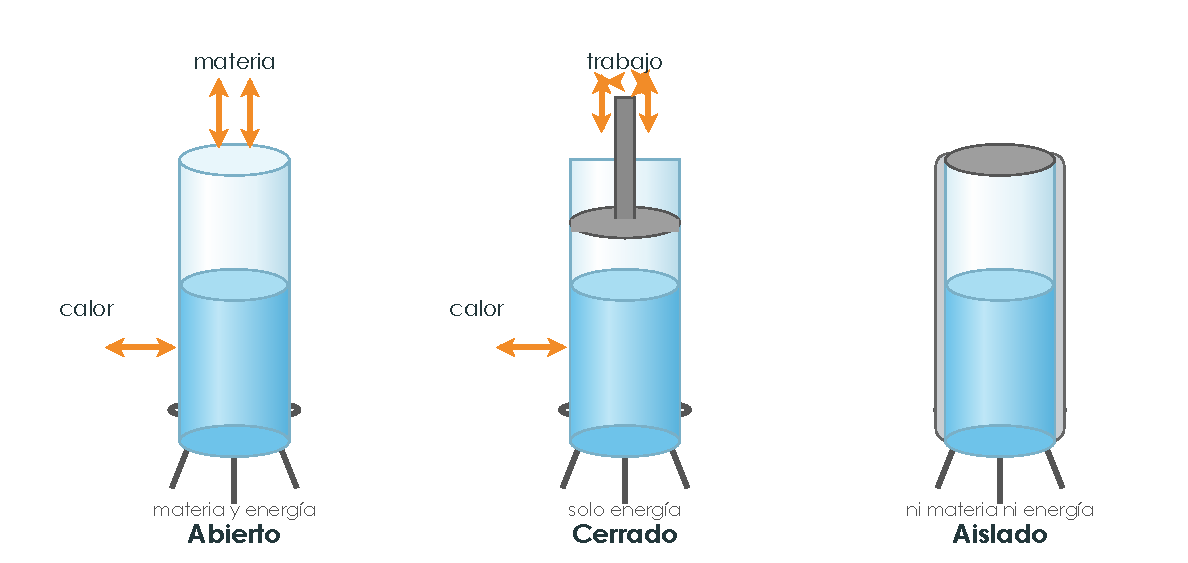
\includegraphics[width=0.7\textwidth]{images/UD13/sistemas}
    \caption{Sistemas abierto, cerrado y aislado.}
    \label{fig:ud13-sistemas}
\end{figure}

Las paredes del sistema determinan qué intercambios son posibles: las \textbf{rígidas} mantienen el volumen constante; las
\textbf{móviles} (como un émbolo) permiten que cambie el volumen e intercambiar trabajo; las \textbf{diatérmanas} dejan pasar el
calor, y las \textbf{adiabáticas} son aislantes térmicos ideales.

\subsection{Variables termodinámicas}

El \textbf{estado} de un sistema queda determinado por los valores de unas magnitudes macroscópicas medibles, las
\textbf{variables termodinámicas}: presión, volumen, temperatura, masa\dots{} Se pueden clasificar de dos formas
(tabla~\ref{tab:ud13-variables}).

\begin{table}[H]
    \centering
    \caption{Clasificación de las variables termodinámicas}
    \vspace{-5pt}
    \begin{tabular}{@{}lL{11cm}@{}}
        \toprule
        \textbf{Tipo} & \textbf{Características y ejemplos} \\
        \midrule
        Extensivas & Dependen de la cantidad de materia: masa \(m\), volumen \(V\), energía interna \(U\). \\[3pt]
        Intensivas & No dependen de la cantidad de materia; tienen un valor en cada punto: presión \(p\), temperatura \(T\),
        densidad \(\rho\). \\[3pt]
        \makecell[l]{Funciones \\ de estado} & Su variación depende solo de los estados inicial y final, no del camino seguido ni del
        tiempo empleado: \(p\), \(V\), \(T\), \(U\). \\[3pt]
        \makecell[l]{Variables de \\ transferencia} & Dependen del proceso seguido para ir de un estado a otro: calor \(Q\) y
        trabajo \(W\). \\
        \bottomrule
    \end{tabular}
    \label{tab:ud13-variables}
\end{table}

Una \textbf{ecuación de estado} relaciona entre sí varias funciones de estado. La más conocida es la de los gases ideales,
\(p\,V = n\,R\,T\), con \(R = \qty{8.31}{\joule\per\mol\per\kelvin} = \qty{0.082}{\atm\litre\per\mol\per\kelvin}\).

\begin{definition}[Proceso termodinámico]
    Es la evolución de un sistema desde un estado inicial \((p_0, V_0, T_0)\) hasta un estado final \((p_f, V_f, T_f)\).
\end{definition}

\begin{exercise}
    Clasifica estos sistemas en abiertos, cerrados o aislados: a) una lata de refresco cerrada; b) un termo de café bien tapado;
    c) una persona; d) una cafetera al fuego; e) un globo de helio atado; f) una planta; g) una nevera portátil cerrada; h) el
    planeta Tierra; i) una bolsa de palomitas en el microondas antes de abrirse.
    \begin{solu}
        \textcolor{red}{Abiertos}: c, d, f. \textcolor{red}{Cerrados}: a, e, h (intercambia energía con el Sol y el espacio, pero
        apenas materia), i. \textcolor{red}{Aislados} (aproximadamente): b, g.
    \end{solu}
\end{exercise}

\begin{exercise}
    Clasifica en extensivas o intensivas: masa, densidad, volumen, temperatura, energía interna, presión, calor específico y
    capacidad calorífica. ¿Se pueden incluir el calor y el trabajo en esta clasificación?
    \begin{solu}
        \textcolor{red}{Extensivas}: masa, volumen, energía interna y capacidad calorífica. \textcolor{red}{Intensivas}: densidad,
        temperatura, presión y calor específico. El calor y el trabajo \textcolor{red}{no}: no son propiedades del estado del
        sistema, sino energía que se transfiere durante un proceso.
    \end{solu}
\end{exercise}

\subsection{Trabajo y calor}

Decimos «¡qué calor hace!» o «este café tiene mucho calor», pero en física es incorrecto: los sistemas \textbf{no tienen} calor ni
trabajo. Calor y trabajo son \textbf{energía en tránsito}, las dos formas en que un sistema puede intercambiar energía con su
entorno:

\begin{itemize}
    \item \textbf{Calor} (\(Q\)): energía transferida debido a una \textbf{diferencia de temperatura} entre el sistema y el entorno.
    \item \textbf{Trabajo} (\(W\)): energía transferida mediante \textbf{fuerzas que producen desplazamientos}, por ejemplo al
    comprimir un gas o al agitar un líquido con unas paletas.
\end{itemize}

Ambos se miden en julios. Para el calor se usa también la \textbf{caloría}.

A mediados del siglo \textsc{xix}, \textbf{James Prescott Joule} demostró que el calor es una forma de energía y no una sustancia (el
«calórico» que se suponía entonces). En su aparato (figura~\ref{fig:ud13-joule}), unas pesas al caer hacen girar unas paletas dentro
del agua; el rozamiento de las paletas con el agua aumenta su temperatura. Midiendo la energía potencial perdida por las pesas y
el aumento de temperatura del agua, Joule obtuvo el \textbf{equivalente mecánico del calor}.

\begin{figure}[H]
    \centering
    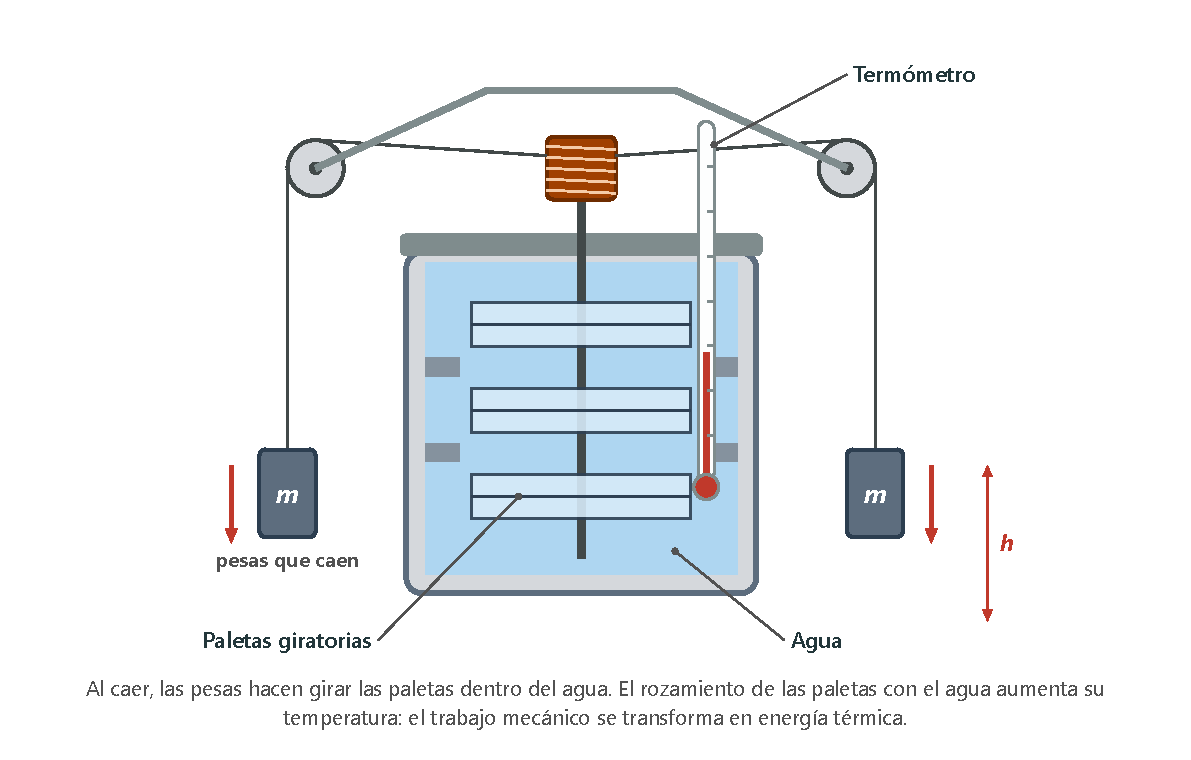
\includegraphics[width=0.65\textwidth]{images/UD13/joule}
    \caption{Experiencia de Joule: el trabajo de las pesas se convierte en energía térmica del agua.}
    \label{fig:ud13-joule}
\end{figure}

\begin{definition}[Caloría]
    Es la energía necesaria para elevar \qty{1}{\degreeCelsius} la temperatura de \qty{1}{\g} de agua a la presión de \qty{1}{\atm}.
    \[ \qty{1}{\calorie} = \qty{4.18}{\joule} \qquad \qty{1}{\joule} = \qty{0.24}{\calorie} \]
\end{definition}

\subsection{Criterio de signos}

Para indicar el sentido de los intercambios de energía, seguiremos el criterio de la \textbf{IUPAC} (llamado a veces «egoísta»,
porque se fija en lo que gana el sistema): \textbf{la energía que entra en el sistema es positiva y la que sale es negativa}
(figura~\ref{fig:ud13-signos}).

\begin{itemize}
    \item \(Q > 0\): el sistema absorbe calor. \(Q < 0\): el sistema cede calor.
    \item \(W > 0\): el entorno realiza trabajo sobre el sistema (compresión). \(W < 0\): el sistema realiza trabajo sobre el
    entorno (expansión).
\end{itemize}

\begin{figure}[H]
    \centering
    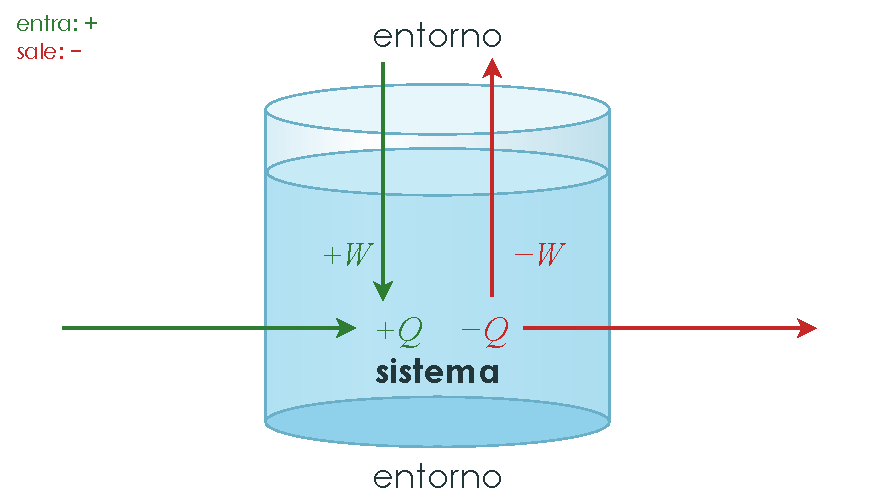
\includegraphics[width=0.45\textwidth]{images/UD13/criterio_signos}
    \caption{Criterio de signos de la IUPAC: lo que entra en el sistema es positivo.}
    \label{fig:ud13-signos}
\end{figure}

\begin{remark}
    En algunos textos de física e ingeniería se usa el criterio contrario para el trabajo (positivo el que hace el sistema), y el
    primer principio se escribe \(\Delta U = Q - W\). Las dos formas son equivalentes si se aplica cada una con su criterio.
\end{remark}

\subsection{Tipos de procesos termodinámicos}

Según si el sistema y el entorno pueden volver o no a su estado inicial, los procesos son:
\begin{itemize}
    \item \textbf{Irreversibles}: transcurren en un solo sentido; no se puede volver atrás sin dejar cambios en el entorno. Todos los
    procesos reales lo son en mayor o menor medida: una combustión, la mezcla de café y leche o el frenado de un coche.
    \item \textbf{Reversibles}: son una idealización; el sistema pasa por una sucesión de estados de equilibrio y se puede invertir
    con un cambio infinitesimal de las condiciones. Algunas reacciones químicas son reversibles, como la síntesis del amoniaco,
    \ch{N2 + 3 H2 <=> 2 NH3}.
\end{itemize}

Según la magnitud que permanece \textbf{constante} (tabla~\ref{tab:ud13-procesos}):

\begin{table}[H]
    \centering
    \caption{Procesos termodinámicos según la magnitud que se mantiene constante}
    \vspace{-5pt}
    \begin{tabular}{@{}llL{8.6cm}@{}}
        \toprule
        \textbf{Proceso} & \textbf{Constante} & \textbf{Ejemplo} \\
        \midrule
        Isobárico & presión, \(p\) & Reacciones en recipientes abiertos (a la presión atmosférica). \\[3pt]
        Isocórico & volumen, \(V\) & Cocinar en una olla exprés cerrada. \\[3pt]
        Isotérmico & temperatura, \(T\) & Fusión de un cubito de hielo: la temperatura se mantiene a \qty{0}{\degreeCelsius}
        hasta que se funde todo. \\[3pt]
        Adiabático & no hay calor, \(Q = 0\) & El gas que sale de un aerosol y se enfría; una compresión muy rápida. \\
        \bottomrule
    \end{tabular}
    \label{tab:ud13-procesos}
\end{table}

\subsection{Equilibrio termodinámico}

Un sistema está en \textbf{equilibrio termodinámico} cuando sus variables (presión, temperatura, composición\dots) no cambian con el
tiempo mientras nada lo perturbe desde el exterior. Si le aportamos calor o trabajo, rompemos ese equilibrio y el sistema evoluciona
hasta alcanzar un nuevo estado de equilibrio.

\begin{example}
    \textbf{¿Qué tipo de proceso es?} Clasifica estos procesos: a) cocer garbanzos en una olla exprés cerrada; b) se pincha una
    rueda y el aire sale de golpe; c) hervir agua en un cazo destapado; d) un cubito de hielo se funde en un vaso de agua con hielo.

    \textbf{Solución.} a) \textbf{Isocórico}: el volumen de la olla no cambia. b) \textbf{Adiabático}: el aire sale tan deprisa que
    no le da tiempo a intercambiar calor (por eso el aire que sale está frío). c) \textbf{Isobárico}: el cazo está abierto a la
    presión atmosférica; además, mientras hierve, la temperatura no cambia. d) \textbf{Isotérmico}: la mezcla de agua y hielo se
    mantiene a \qty{0}{\degreeCelsius}.
\end{example}

\begin{exercise}
    Escribe dos ejemplos de procesos reversibles y dos de procesos irreversibles de la vida cotidiana.
    \begin{solu}
        \textcolor{red}{Respuesta abierta}. Casi reversibles: fundir y volver a congelar un cubito; comprimir muy despacio el aire
        de una jeringa y dejarlo expandirse. Irreversibles: quemar un papel, romper un vaso, disolver azúcar en el café.
    \end{solu}
\end{exercise}

\begin{exercise}
    Explica con tus palabras el criterio de signos para el calor y el trabajo. Un gas encerrado en un cilindro recibe
    \qty{300}{\joule} de calor y empuja el émbolo realizando un trabajo de \qty{120}{\joule}. ¿Qué signos tienen \(Q\) y \(W\)?
    \begin{solu}
        Lo que entra en el sistema es positivo y lo que sale, negativo. \(Q = \textcolor{red}{\qty{+300}{\joule}}\) (entra calor);
        \(W = \textcolor{red}{\qty{-120}{\joule}}\) (el gas hace trabajo sobre el entorno y pierde energía).
    \end{solu}
\end{exercise}

\begin{exercise}
    ¿Es correcto decir que «la sopa tiene mucho calor»? ¿Cómo debería decirse?
    \begin{solu}
        \textcolor{red}{No}: los cuerpos no tienen calor, el calor es energía en tránsito. Debería decirse que la sopa
        \textcolor{red}{está a una temperatura alta} (o que tiene mucha energía interna) y que \textcolor{red}{puede ceder calor}
        a la boca.
    \end{solu}
\end{exercise}

%========================================================================================
\section{El principio cero de la termodinámica}\label{sec:ud13-principio-cero}
%========================================================================================

\subsection{Temperatura}

Calor y temperatura están relacionados, pero no son lo mismo: un cuerpo \textbf{tiene} una temperatura, pero no contiene calor.

\begin{definition}[Temperatura]
    Es la magnitud que mide la \textbf{energía cinética media} de las partículas de un sistema. Si aportamos energía a un sistema,
    sus partículas se mueven más deprisa en promedio y su temperatura aumenta (figura~\ref{fig:ud13-particulas}).
\end{definition}

\begin{figure}[H]
    \centering
    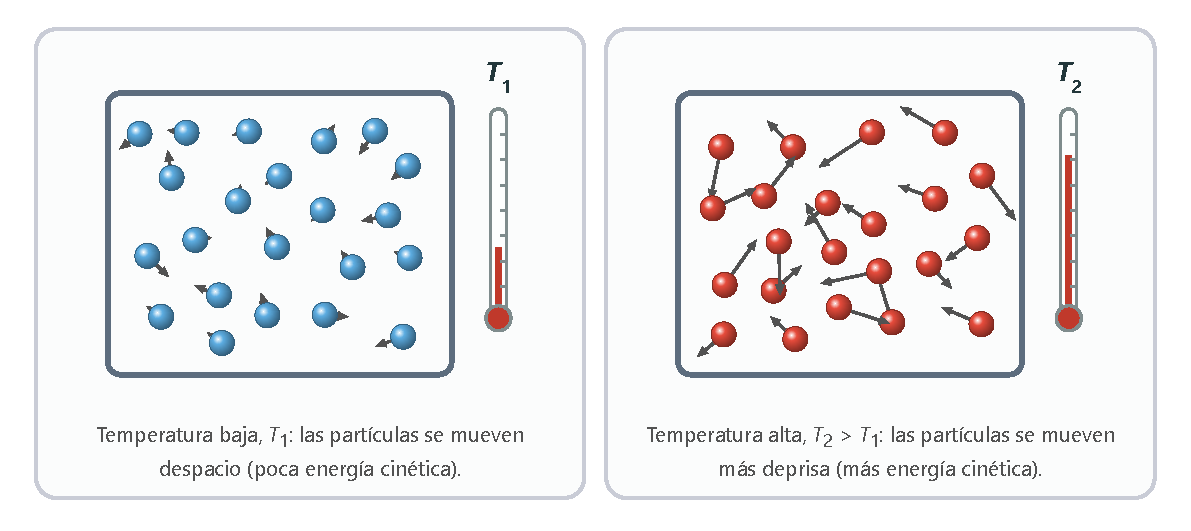
\includegraphics[width=0.8\textwidth]{images/UD13/particulas_temperatura}
    \caption{A mayor temperatura, mayor energía cinética media de las partículas.}
    \label{fig:ud13-particulas}
\end{figure}

Para medir la temperatura usamos \textbf{termómetros}, basados en \textbf{propiedades termométricas}, magnitudes que cambian con la
temperatura: la longitud de una columna de líquido, la presión de un gas a volumen constante, la resistencia eléctrica de un metal
o la radiación infrarroja que emite un cuerpo. La unidad de temperatura en el SI es el \textbf{kelvin} (K), aunque en la vida
diaria usamos el grado Celsius (figura~\ref{fig:ud13-escalas}):
\begin{itemize}
    \item \textbf{Escala Celsius}: asigna \qty{0}{\degreeCelsius} a la fusión del hielo y \qty{100}{\degreeCelsius} a la ebullición
    del agua a \qty{1}{\atm}, y divide el intervalo en 100 partes.
    \item \textbf{Escala Kelvin} o absoluta: su cero es el \textbf{cero absoluto}, la temperatura más baja posible, en la que la
    agitación de las partículas sería mínima; equivale a \qty{-273.15}{\degreeCelsius}. No tiene valores negativos.
\end{itemize}
\[ T\,(\unit{\kelvin}) = t\,(\unit{\degreeCelsius}) + \num{273.15} \]
Como el tamaño del grado es el mismo en las dos escalas, una \textbf{variación} de temperatura vale lo mismo en kelvin que en grados
Celsius: \(\Delta T\,(\unit{\kelvin}) = \Delta t\,(\unit{\degreeCelsius})\). En los cálculos se suele redondear a 273.

\begin{figure}[H]
    \centering
    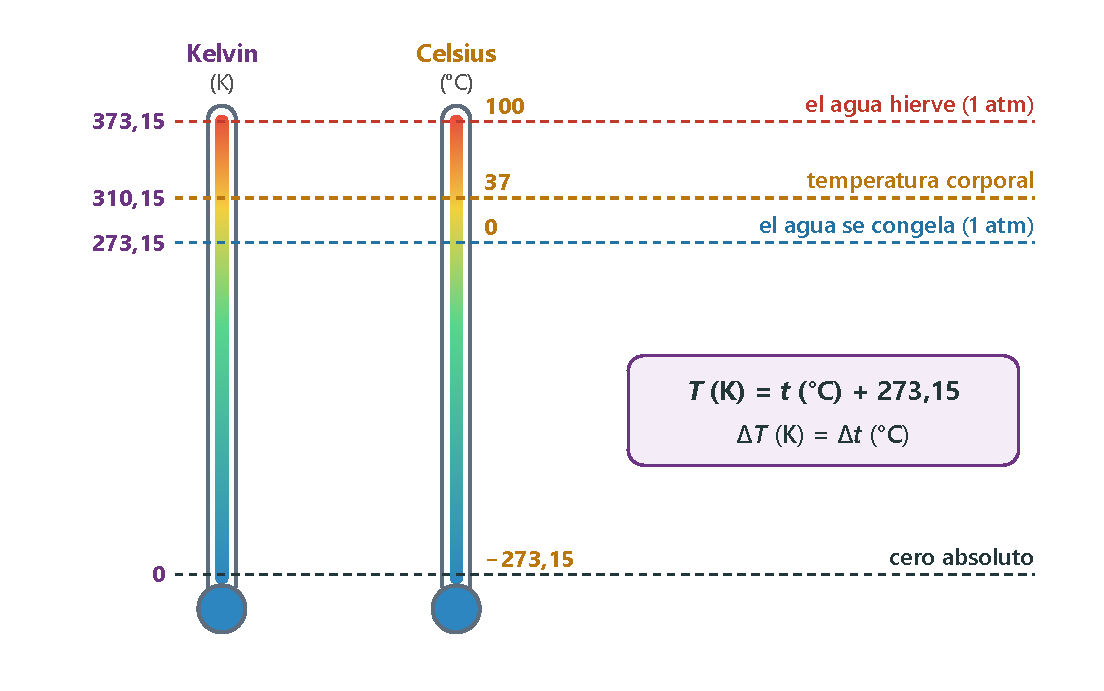
\includegraphics[width=0.7\textwidth]{images/UD13/escalas_temperatura}
    \caption{Relación entre las escalas Kelvin y Celsius.}
    \label{fig:ud13-escalas}
\end{figure}

\begin{example}
    \textbf{Cambios de escala.} a) Expresa en kelvin la temperatura de una persona con fiebre, \qty{38.5}{\degreeCelsius}.
    b) El nitrógeno líquido hierve a \qty{77}{\kelvin}: ¿a cuántos grados Celsius? c) Un día de verano la temperatura pasa de
    \qty{20}{\degreeCelsius} a \qty{38}{\degreeCelsius}; ¿cuánto vale la variación en kelvin?

    \textbf{Solución.} a) \(T = \num{38.5} + \num{273.15} = \qty{311.65}{\kelvin}\). b) \(t = 77 - \num{273.15} =
    \qty{-196.15}{\degreeCelsius}\). c) \(\Delta T = (38 + 273) - (20 + 273) = \qty{18}{\kelvin}\), igual que en grados Celsius.
\end{example}

\subsection{Equilibrio térmico y principio cero}

Cuando dos cuerpos a distinta temperatura se ponen en contacto, el caliente se enfría y el frío se calienta: el más caliente
cede energía en forma de calor al más frío hasta que sus temperaturas se igualan. Entonces ya no hay intercambio neto de energía y
se dice que han alcanzado el \textbf{equilibrio térmico} (figura~\ref{fig:ud13-equilibrio}). Lo que pasa de un cuerpo a otro es
siempre calor: el «frío» no se transmite.

\begin{figure}[H]
    \centering
    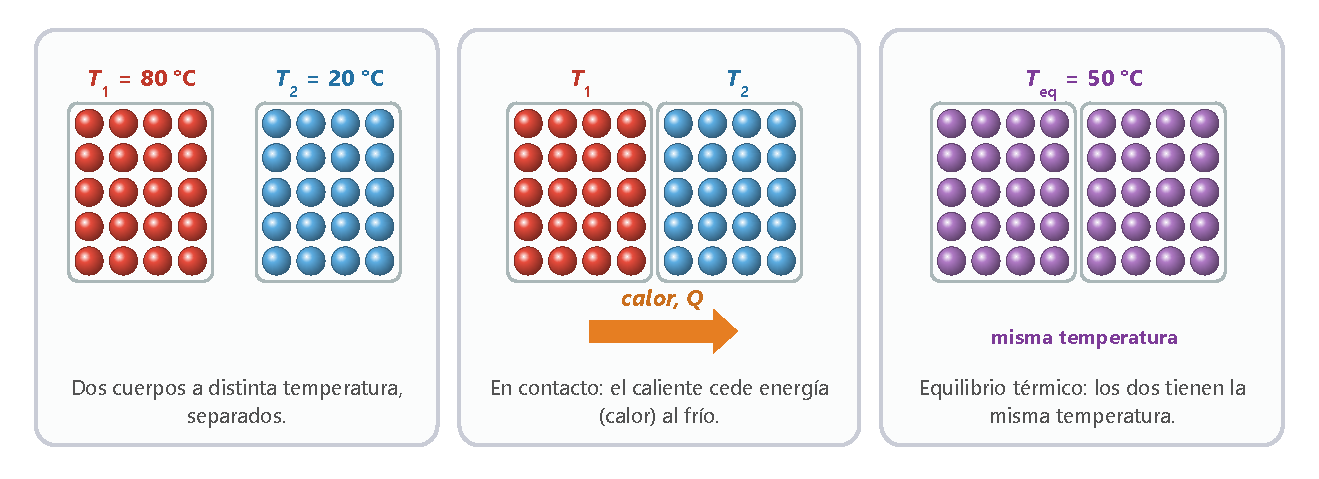
\includegraphics[width=0.85\textwidth]{images/UD13/equilibrio_termico}
    \caption{Dos cuerpos en contacto alcanzan el equilibrio térmico.}
    \label{fig:ud13-equilibrio}
\end{figure}

\begin{definition}[Principio cero de la termodinámica]
    Si dos sistemas A y B están, cada uno por separado, en equilibrio térmico con un tercero C, también están en equilibrio
    térmico entre sí (figura~\ref{fig:ud13-cero}):
    \[ T_A = T_C \ \text{y} \ T_B = T_C \ \Rightarrow \ T_A = T_B \]
\end{definition}

\begin{figure}[H]
    \centering
    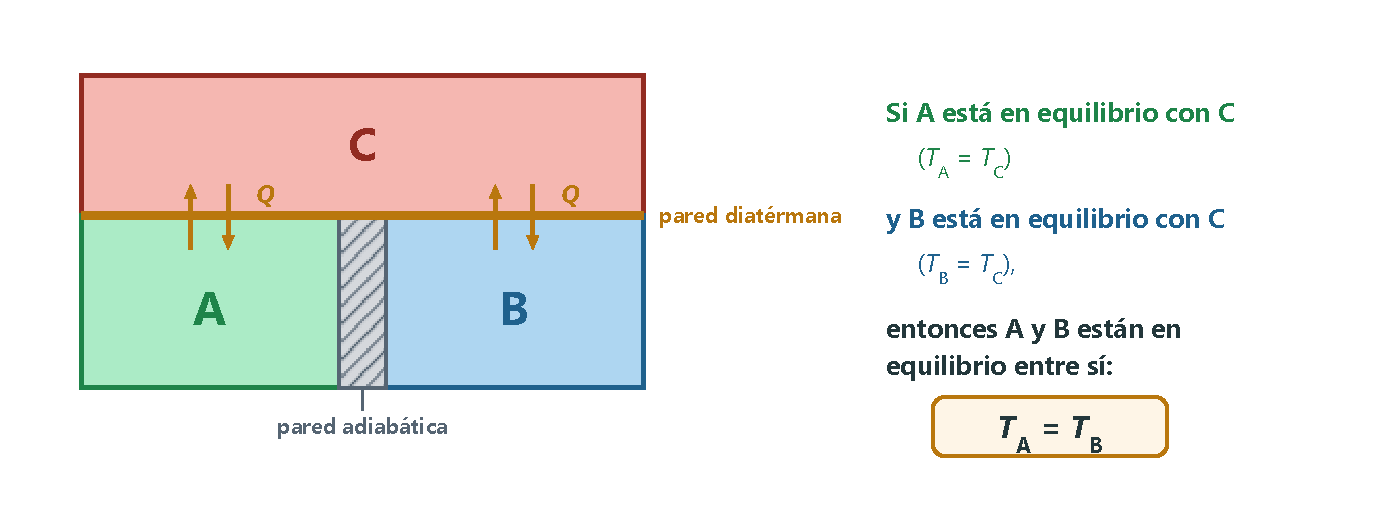
\includegraphics[width=0.8\textwidth]{images/UD13/principio_cero}
    \caption{Principio cero: el equilibrio térmico es transitivo.}
    \label{fig:ud13-cero}
\end{figure}

Parece una obviedad, pero es lo que da sentido a los termómetros: el termómetro es el sistema C, que se pone en equilibrio con
cada cuerpo y nos permite comparar sus temperaturas sin ponerlos en contacto. Se llama «cero» porque se formuló después del
primer y del segundo principio, pero es lógicamente anterior a ellos.

\begin{exercise}
    Después de tres horas en clase, ¿están todos los objetos del aula a la misma temperatura? Entonces, ¿por qué la pata metálica
    de la silla parece más fría que el tablero de madera de la mesa?
    \begin{solu}
        \textcolor{red}{Sí}, si el aula lleva tiempo a temperatura estable, todos han alcanzado el equilibrio térmico con el aire.
        El metal parece más frío porque es \textcolor{red}{mejor conductor} y extrae calor de la mano más deprisa: nuestra
        sensación no mide la temperatura, sino la rapidez con que perdemos calor.
    \end{solu}
\end{exercise}

\begin{exercise}
    ¿Hay equilibrio térmico en estas situaciones? Justifícalo. a) Una bolsa de guisantes que lleva días en el congelador. b) Un
    café que se nos olvidó en la mesa hace dos horas. c) Un cubito de hielo que acabamos de echar a un refresco. d) Una persona
    que nada durante una hora en una piscina.
    \begin{solu}
        a) \textcolor{red}{Sí}, con el interior del congelador. b) \textcolor{red}{Sí}, ya está a la temperatura de la cocina. c)
        \textcolor{red}{No}: el refresco cede calor al hielo. d) \textcolor{red}{No}: el cuerpo regula su temperatura en torno a
        \qty{37}{\degreeCelsius} y cede calor continuamente al agua, más fría.
    \end{solu}
\end{exercise}

\begin{exercise}
    a) La superficie del Sol está a unos \qty{5780}{\kelvin}. Exprésalo en grados Celsius. b) La temperatura más baja medida en la
    Antártida es de \qty{-89.2}{\degreeCelsius}. Exprésala en kelvin.
    \begin{solu}
        a) \(\textcolor{red}{\qty{5507}{\degreeCelsius}}\). b) \(\textcolor{red}{\qty{183.95}{\kelvin}}\) (unos \qty{184}{\kelvin}).
    \end{solu}
\end{exercise}

%========================================================================================
\section{Intercambio de energía en forma de calor}\label{sec:ud13-calor}
%========================================================================================

\subsection{Mecanismos de propagación del calor}

El calor se propaga de tres formas, que suelen darse a la vez (figura~\ref{fig:ud13-mecanismos}):

\begin{itemize}
    \item \textbf{Conducción}: las partículas más agitadas chocan con sus vecinas y les pasan energía cinética, sin que haya
    transporte de materia. Es típica de los sólidos en contacto. Cada material tiene una \textbf{conductividad térmica}: los
    metales son \textbf{buenos conductores}, y el plástico, la madera, el corcho o el aire son \textbf{malos conductores} o
    \textbf{aislantes}.
    \item \textbf{Convección}: la parte caliente de un fluido se dilata, se hace menos densa y asciende, mientras la fría, más
    densa, desciende. Se forman \textbf{corrientes de convección} que transportan materia y energía. Es típica de líquidos y
    gases: las corrientes oceánicas, la brisa marina o el globo aerostático.
    \item \textbf{Radiación}: la energía se transmite mediante \textbf{ondas electromagnéticas}, sobre todo radiación
    \textbf{infrarroja}, y no necesita un medio material: se propaga incluso en el vacío. Así nos llega la energía del Sol, que es
    la principal fuente de energía de la Tierra. Las cámaras termográficas detectan esta radiación.
\end{itemize}

\begin{figure}[H]
    \centering
    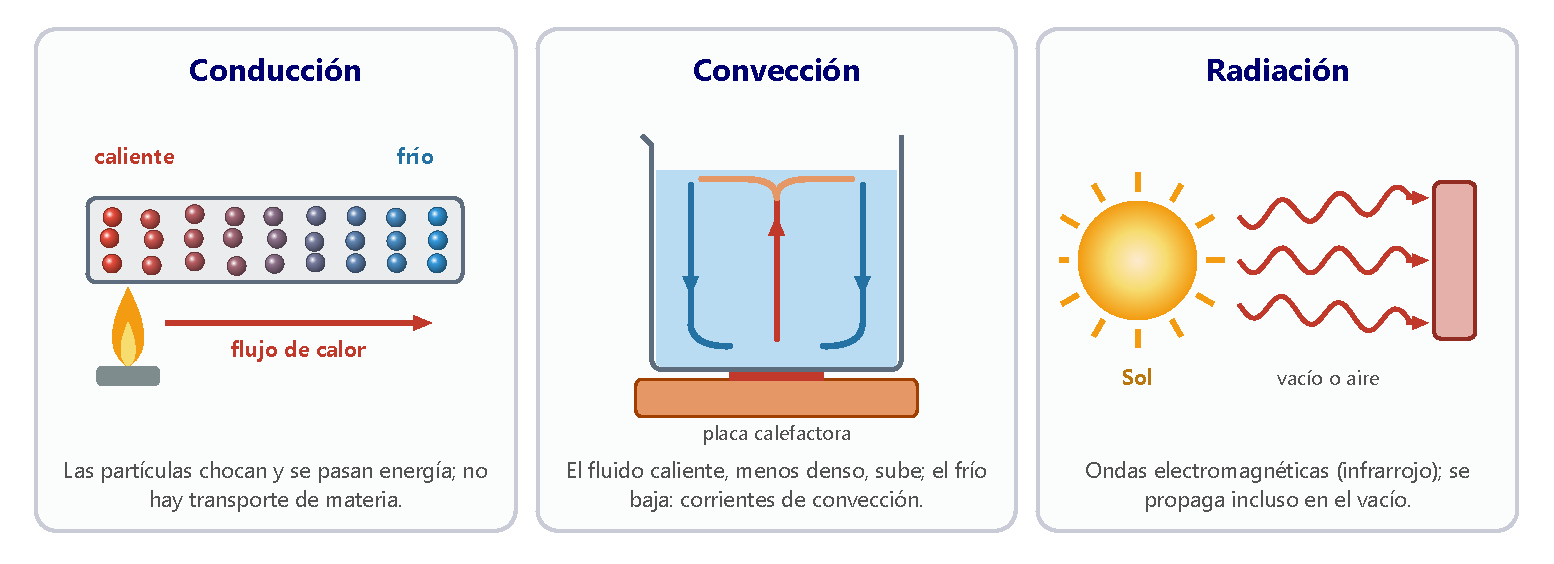
\includegraphics[width=\textwidth]{images/UD13/mecanismos_calor}
    \caption{Mecanismos de propagación del calor.}
    \label{fig:ud13-mecanismos}
\end{figure}

\begin{example}
    \textbf{¿Qué mecanismo es?} Indica el mecanismo de propagación del calor en cada caso: a) se calienta el mango de una cuchara
    metálica dentro de una sopa; b) sentimos el calor de una hoguera en la cara aunque el aire esté frío; c) durante el día, la
    brisa sopla del mar hacia la tierra.

    \textbf{Solución.} a) \textbf{Conducción}: la energía pasa de partícula en partícula a lo largo del metal. b)
    \textbf{Radiación}: la hoguera emite radiación infrarroja, que no necesita calentar el aire. c) \textbf{Convección}: la tierra
    se calienta más que el mar; el aire caliente sobre la tierra sube y su lugar lo ocupa el aire más fresco del mar.
\end{example}

\begin{exercise}
    ¿Qué mecanismo de propagación del calor predomina en cada caso? a) Un radiador calienta una habitación. b) Planchamos una
    camisa. c) Un panel solar térmico calienta agua. d) Las corrientes del océano Atlántico. e) Nos quemamos al tocar una sartén.
    \begin{solu}
        a) \textcolor{red}{Convección} (y algo de radiación). b) \textcolor{red}{Conducción}. c) \textcolor{red}{Radiación} (y
        convección del agua dentro del circuito). d) \textcolor{red}{Convección}. e) \textcolor{red}{Conducción}.
    \end{solu}
\end{exercise}

\begin{exercise}
    ¿Por qué los aparatos de aire acondicionado se colocan en lo alto de las paredes y los radiadores, cerca del suelo?
    \begin{solu}
        Por la \textcolor{red}{convección}: el aire frío, más denso, desciende desde el aparato y enfría toda la habitación; el aire
        caliente del radiador, menos denso, sube y se forman corrientes que reparten el calor.
    \end{solu}
\end{exercise}

\subsection{Calor y variación de temperatura}

Si suministramos la misma cantidad de calor a dos cuerpos de igual masa, sus temperaturas no aumentan lo mismo. La
\textbf{capacidad calorífica} \(C\) de un cuerpo es el calor que necesita para que su temperatura suba \qty{1}{\kelvin}:
\[ C = \frac{Q}{\Delta T} \qquad \text{(en \unit{\joule\per\kelvin})} \]
Depende de la \textbf{masa} y de la \textbf{naturaleza} del material, \(C = m\,c_e\), donde \(c_e\) es el calor específico.

\begin{definition}[Calor específico]
    El \textbf{calor específico} \(c_e\) de una sustancia es el calor que hay que transferir a la unidad de masa para que su
    temperatura aumente \qty{1}{\kelvin}. Se mide en \unit{\joule\per\kg\per\kelvin}, aunque es muy habitual
    \unit{\calorie\per\g\per\degreeCelsius}. El calor intercambiado al variar la temperatura es:
    \[ Q = m\,c_e\,\Delta T = m\,c_e\,(T_f - T_i) \]
\end{definition}

Si \(T_f > T_i\), \(Q > 0\) (el cuerpo absorbe calor); si \(T_f < T_i\), \(Q < 0\) (lo cede). Cuanto mayor es el calor específico,
más energía hace falta para calentar la sustancia y más tarda en enfriarse. El agua tiene un calor específico muy alto
(tabla~\ref{tab:ud13-calor-especifico}): por eso los mares suavizan el clima de las zonas costeras y el agua se usa para
refrigerar motores.

\begin{table}[H]
    \centering
    \caption{Calor específico de algunas sustancias (a \qty{25}{\degreeCelsius} y \qty{1}{\atm})}
    \vspace{-5pt}
    \begin{tabular}{@{}lcc@{}}
        \toprule
        \textbf{Sustancia} & \makecell{\(c_e\) \\ (\unit{\joule\per\kg\per\kelvin})} & \makecell{\(c_e\) \\ (\unit{\calorie\per\g\per\degreeCelsius})} \\
        \midrule
        Agua (líquida) & 4180 & 1 \\[3pt]
        Hielo & 2090 & \num{0.50} \\[3pt]
        Vapor de agua & 2010 & \num{0.48} \\[3pt]
        Etanol & 2420 & \num{0.58} \\[3pt]
        Aluminio & 900 & \num{0.215} \\[3pt]
        Vidrio & 840 & \num{0.20} \\[3pt]
        Hierro & 460 & \num{0.11} \\[3pt]
        Cobre & 385 & \num{0.093} \\[3pt]
        Plata & 234 & \num{0.056} \\[3pt]
        Plomo & 130 & \num{0.031} \\
        \bottomrule
    \end{tabular}
    \label{tab:ud13-calor-especifico}
\end{table}

\begin{remark}
    El calor específico no es una función de estado, porque depende de cómo se caliente la sustancia. En los gases se distingue
    el calor específico molar \textbf{a presión constante}, \(c_p\), y \textbf{a volumen constante}, \(c_v\), y se usa el mol como
    cantidad de materia: \(Q = n\,c_{p}\,\Delta T\) o \(Q = n\,c_{v}\,\Delta T\), con \(c\) en \unit{\joule\per\mol\per\kelvin}.
\end{remark}

\begin{example}
    \textbf{Agua para un té.} a) ¿Qué calor hay que suministrar a \qty{300}{\g} de agua para calentarla de \qty{20}{\degreeCelsius} a
    \qty{90}{\degreeCelsius}? Exprésalo en julios y en kilocalorías. b) ¿Qué calor pierden \qty{500}{\g} de agua al enfriarse en
    la nevera de \qty{30}{\degreeCelsius} a \qty{5}{\degreeCelsius}?

    \textbf{Solución.} a) \(Q = m\,c_e\,\Delta T = \num{0.300} \cdot 4180 \cdot (90 - 20) = \qty{8.78e4}{\joule} = \qty{87.8}{\kilo\joule}\).
    En calorías: \(Q = 300 \cdot 1 \cdot 70 = \qty{21000}{\calorie} = \qty{21}{\kilo\calorie}\).

    b) \(Q = \num{0.500} \cdot 4180 \cdot (5 - 30) = \qty{-5.23e4}{\joule} = \qty{-52.3}{\kilo\joule}\). El signo negativo indica
    que el agua cede calor.
\end{example}

\begin{exercise}
    Se suministran \qty{1500}{\calorie} a \qty{250}{\g} de cobre que están a \qty{18}{\degreeCelsius}. ¿Qué temperatura alcanza?
    \begin{solu}
        \(\Delta T = \dfrac{Q}{m\,c_e} = \dfrac{1500}{250 \cdot \num{0.093}} = \qty{64.5}{\degreeCelsius}\);
        \(T_f = \textcolor{red}{\qty{82.5}{\degreeCelsius}}\).
    \end{solu}
\end{exercise}

\begin{exercise}
    ¿Qué calor hay que suministrar a una pieza de hierro de \qty{800}{\kg} para calentarla desde \qty{20}{\degreeCelsius} hasta
    \qty{1200}{\degreeCelsius} para forjarla? Exprésalo en kilocalorías y en julios.
    \begin{solu}
        \(Q = \num{8e5}~\mathrm{g} \cdot \num{0.11} \cdot 1180 = \qty{1.04e8}{\calorie} = \textcolor{red}{\qty{1.04e5}{\kilo\calorie}}
        = \textcolor{red}{\qty{4.34e8}{\joule}}\).
    \end{solu}
\end{exercise}

\paragraph{Equilibrio térmico y calorimetría.} Si mezclamos dos cuerpos a distinta temperatura en un recipiente aislado
(\textbf{calorímetro}), el calor que cede el caliente lo absorbe el frío, hasta que ambos alcanzan la misma temperatura final
\(T_{eq}\) (figura~\ref{fig:ud13-calorimetro}). Como no se pierde energía:
\[ Q_{\text{cedido}} + Q_{\text{absorbido}} = 0 \ \Rightarrow \ m_1\,c_1\,(T_{eq} - T_1) + m_2\,c_2\,(T_{eq} - T_2) = 0 \]

\begin{figure}[H]
    \centering
    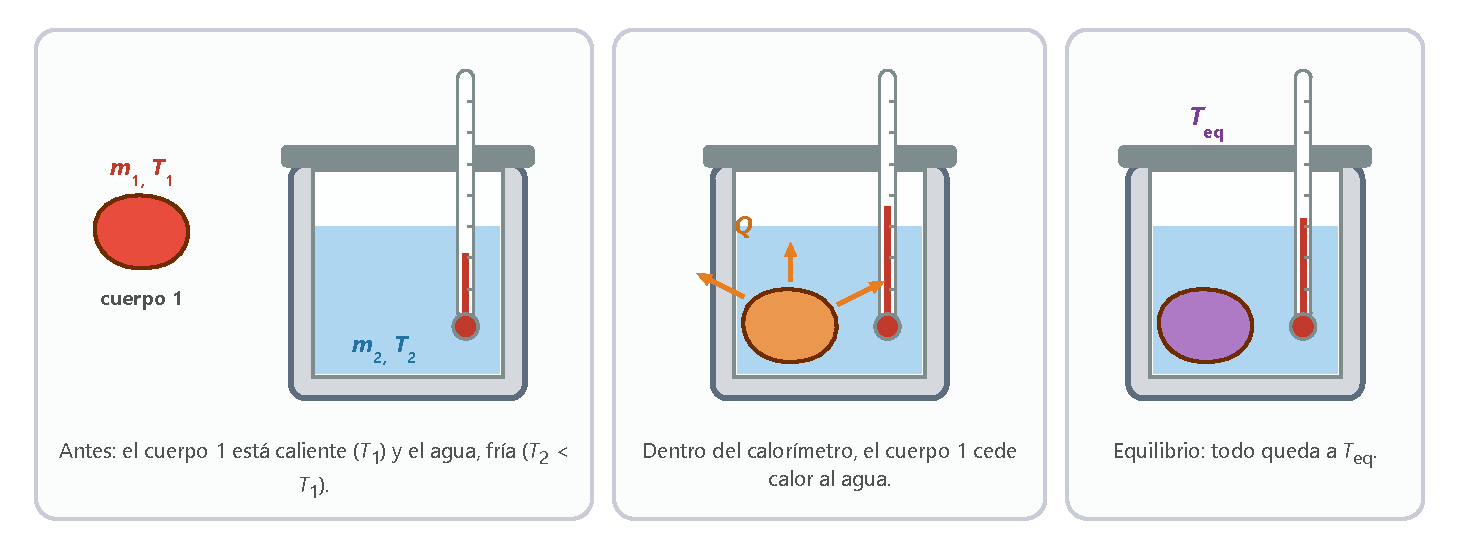
\includegraphics[width=0.85\textwidth]{images/UD13/balance_calorimetro}
    \caption{En un calorímetro, el calor cedido por el cuerpo caliente lo absorbe el agua.}
    \label{fig:ud13-calorimetro}
\end{figure}

\begin{example}
    \textbf{Templar el agua del baño.} Se mezclan \qty{1.2}{\litre} de agua a \qty{15}{\degreeCelsius} con \qty{0.8}{\litre} de
    agua a \qty{70}{\degreeCelsius} en un recipiente aislado. Calcula la temperatura final y el calor que intercambia cada parte.
    Densidad del agua: \qty{1}{\kg\per\litre}.

    \textbf{Solución.} Las masas son \qty{1.2}{\kg} y \qty{0.8}{\kg}. Como el calor específico es el mismo, se simplifica:
    \[ \num{1.2}\,(T - 15) + \num{0.8}\,(T - 70) = 0 \Rightarrow T = \frac{\num{1.2} \cdot 15 + \num{0.8} \cdot 70}{2} = \qty{37}{\degreeCelsius} \]
    Agua fría: \(Q_1 = \num{1.2} \cdot 4180 \cdot (37 - 15) = \qty{+1.10e5}{\joule}\) (absorbe). Agua caliente: \(Q_2 =
    \num{0.8} \cdot 4180 \cdot (37 - 70) = \qty{-1.10e5}{\joule}\) (cede la misma cantidad).
\end{example}

\begin{exercise}
    Se mezclan \qty{5}{\kg} de agua a \qty{80}{\degreeCelsius} con \qty{10}{\kg} de agua a \qty{20}{\degreeCelsius}. ¿Cuál es la
    temperatura final? ¿Qué calor cede el agua caliente?
    \begin{solu}
        \(T = \dfrac{5 \cdot 80 + 10 \cdot 20}{15} = \textcolor{red}{\qty{40}{\degreeCelsius}}\);
        \(Q = 5 \cdot 4180 \cdot (40 - 80) = \textcolor{red}{\qty{-8.36e5}{\joule}}\).
    \end{solu}
\end{exercise}

\subsection{Cambios de estado}

Mientras una sustancia pura cambia de estado, su temperatura \textbf{no varía} aunque le sigamos dando calor: toda la energía se
emplea en vencer las fuerzas entre las partículas. Los cambios de estado son procesos \textbf{isotérmicos} y reversibles: la energía
absorbida en un sentido (por ejemplo, al fundir) es la misma que se cede en el sentido contrario (al solidificar)
(figura~\ref{fig:ud13-cambios}).

\begin{figure}[H]
    \centering
    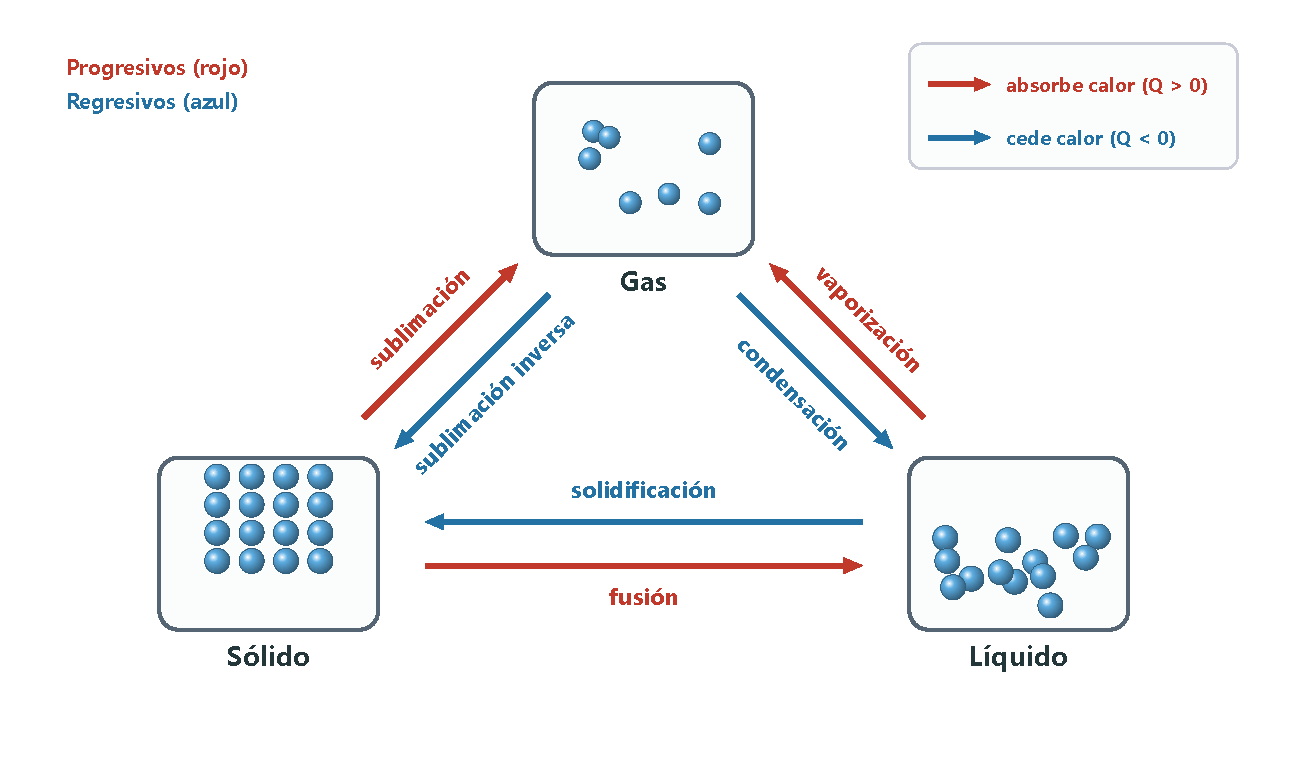
\includegraphics[width=0.8\textwidth]{images/UD13/cambios_estado}
    \caption{Cambios de estado progresivos (absorben calor) y regresivos (lo ceden).}
    \label{fig:ud13-cambios}
\end{figure}

\begin{definition}[Calor latente]
    El \textbf{calor latente} \(L\) de un cambio de estado es la energía que hay que suministrar a la unidad de masa de una
    sustancia para que cambie de estado a temperatura y presión constantes. Hay calor latente de \textbf{fusión} \(L_f\), de
    \textbf{vaporización} \(L_v\) y de \textbf{sublimación} \(L_s\). Se mide en \unit{\joule\per\kg} (también en
    \unit{\calorie\per\g}). El calor intercambiado es:
    \[ |Q| = m\,L \]
\end{definition}

En un cambio \textbf{progresivo} (fusión, vaporización, sublimación) el sistema absorbe energía, \(Q > 0\); en uno
\textbf{regresivo} (solidificación, condensación, sublimación inversa) la cede, \(Q < 0\).

\begin{table}[H]
    \centering
    \caption{Temperaturas de cambio de estado (a \qty{1}{\atm}) y calores latentes}
    \vspace{-5pt}
    \begin{tabular}{@{}lcccc@{}}
        \toprule
        \textbf{Sustancia} & \makecell{\textbf{Fusión} \\ (\unit{\degreeCelsius})} & \makecell{\(L_f\) \\ (\unit{\kilo\joule\per\kg})} &
        \makecell{\textbf{Ebullición} \\ (\unit{\degreeCelsius})} & \makecell{\(L_v\) \\ (\unit{\kilo\joule\per\kg})} \\
        \midrule
        Agua & 0 & 334 & 100 & 2260 \\[3pt]
        Etanol & \num{-114} & 104 & 78 & 854 \\[3pt]
        Mercurio & \num{-39} & 11 & 357 & 296 \\[3pt]
        Plomo & 327 & 25 & 1750 & 871 \\[3pt]
        Hierro & 1538 & 247 & 2862 & 6090 \\
        \bottomrule
    \end{tabular}
    \label{tab:ud13-latentes}
\end{table}

\begin{example}
    \textbf{Del congelador al vapor.} Calcula la energía necesaria para transformar \qty{200}{\g} de hielo a \qty{-10}{\degreeCelsius}
    en vapor de agua a \qty{100}{\degreeCelsius}. Datos: \(c_{\text{hielo}} = \qty{2090}{\joule\per\kg\per\kelvin}\),
    \(c_{\text{agua}} = \qty{4180}{\joule\per\kg\per\kelvin}\), \(L_f = \qty{3.34e5}{\joule\per\kg}\), \(L_v = \qty{2.26e6}{\joule\per\kg}\).

    \textbf{Solución.} Hay cuatro etapas (figura~\ref{fig:ud13-calentamiento}):

    1. Calentar el hielo hasta \qty{0}{\degreeCelsius}: \(Q_1 = \num{0.2} \cdot 2090 \cdot 10 = \qty{4180}{\joule}\).

    2. Fundir el hielo: \(Q_2 = \num{0.2} \cdot \num{3.34e5} = \qty{66800}{\joule}\).

    3. Calentar el agua hasta \qty{100}{\degreeCelsius}: \(Q_3 = \num{0.2} \cdot 4180 \cdot 100 = \qty{83600}{\joule}\).

    4. Vaporizar el agua: \(Q_4 = \num{0.2} \cdot \num{2.26e6} = \qty{452000}{\joule}\).

    En total, \(Q = Q_1 + Q_2 + Q_3 + Q_4 = \qty{6.07e5}{\joule} = \qty{607}{\kilo\joule}\). Fíjate en que la vaporización se lleva
    tres cuartas partes de la energía.
\end{example}

\begin{figure}[H]
    \centering
    \begin{tikzpicture}
        \begin{axis}[grafica, width=0.75\linewidth, height=6cm, xlabel={Calor suministrado (kJ)}, ylabel={\(t\) (\unit{\degreeCelsius})},
            xmin=0, xmax=650, ymin=-20, ymax=130, xtick={0,4.2,71,154.6,606.6}, xticklabels={0,,71,155,607},
            ytick={-10,0,100}]
            \addplot[very thick, ocre] coordinates {(0,-10) (4.18,0) (70.98,0) (154.58,100) (606.58,100) (630,112)};
            \node[font=\scriptsize, anchor=south] at (axis cs:37,2) {fusión};
            \node[font=\scriptsize, anchor=south, align=center] at (axis cs:380,102) {ebullición (agua + vapor)};
            \node[font=\scriptsize, anchor=west] at (axis cs:118,40) {agua};
            \node[font=\scriptsize, anchor=west] at (axis cs:8,-10) {hielo};
            \node[font=\scriptsize, anchor=south east] at (axis cs:640,112) {vapor};
        \end{axis}
    \end{tikzpicture}
    \caption{Curva de calentamiento de \qty{200}{\g} de hielo: durante los cambios de estado la temperatura no varía.}
    \label{fig:ud13-calentamiento}
\end{figure}

\begin{exercise}
    ¿Qué energía hay que suministrar para vaporizar \qty{80}{\g} de agua que ya está a \qty{100}{\degreeCelsius}?
    \(L_v = \qty{540}{\calorie\per\g}\).
    \begin{solu}
        \(Q = m\,L_v = 80 \cdot 540 = \textcolor{red}{\qty{43200}{\calorie}} = \qty{43.2}{\kilo\calorie} \approx \qty{181}{\kilo\joule}\).
    \end{solu}
\end{exercise}

\begin{exercise}
    ¿Por qué una quemadura con vapor de agua a \qty{100}{\degreeCelsius} es más grave que una con agua líquida a
    \qty{100}{\degreeCelsius}?
    \begin{solu}
        Porque el vapor, al condensarse sobre la piel, cede además su \textcolor{red}{calor latente de vaporización} (unos
        \qty{2260}{\joule} por gramo), que es mucho mayor que el calor que cede el agua al enfriarse.
    \end{solu}
\end{exercise}

\subsection{Dilatación térmica}

Al calentar un cuerpo, sus partículas se agitan más y se separan: aumentan sus dimensiones. Es la \textbf{dilatación térmica}; el
proceso contrario es la \textbf{contracción}. Según las dimensiones que importan, distinguimos (tabla~\ref{tab:ud13-dilatacion}):

\begin{table}[H]
    \centering
    \caption{Tipos de dilatación}
    \vspace{-5pt}
    \begin{tabular}{@{}lL{4.3cm}cL{4.4cm}@{}}
        \toprule
        \textbf{Dilatación} & \textbf{Se da en\dots} & \textbf{Expresión} & \textbf{Coeficiente} \\
        \midrule
        Lineal & varillas, cables, raíles (domina la longitud) & \(L = L_0\,(1 + \lambda\,\Delta T)\) & \(\lambda\), dilatación
        lineal \\[3pt]
        Superficial & placas y láminas & \(S = S_0\,(1 + \beta\,\Delta T)\) & \(\beta \approx 2\lambda\), dilatación superficial \\[3pt]
        Cúbica & cuerpos con tres dimensiones, líquidos y gases & \(V = V_0\,(1 + \gamma\,\Delta T)\) & \(\gamma \approx 3\lambda\),
        dilatación cúbica \\
        \bottomrule
    \end{tabular}
    \label{tab:ud13-dilatacion}
\end{table}

Los coeficientes de dilatación son característicos de cada material y se miden en \unit{\per\kelvin} (o
\unit{\per\degreeCelsius}): son el aumento relativo de longitud, superficie o volumen por cada grado. Los gases se dilatan mucho
más que los líquidos, y estos más que los sólidos. \textbf{Gay-Lussac} comprobó que, a presión constante, todos los gases tienen
prácticamente el mismo coeficiente: \(\gamma \approx \frac{1}{273}~\unit{\per\degreeCelsius}\).

\begin{figure}[H]
    \centering
    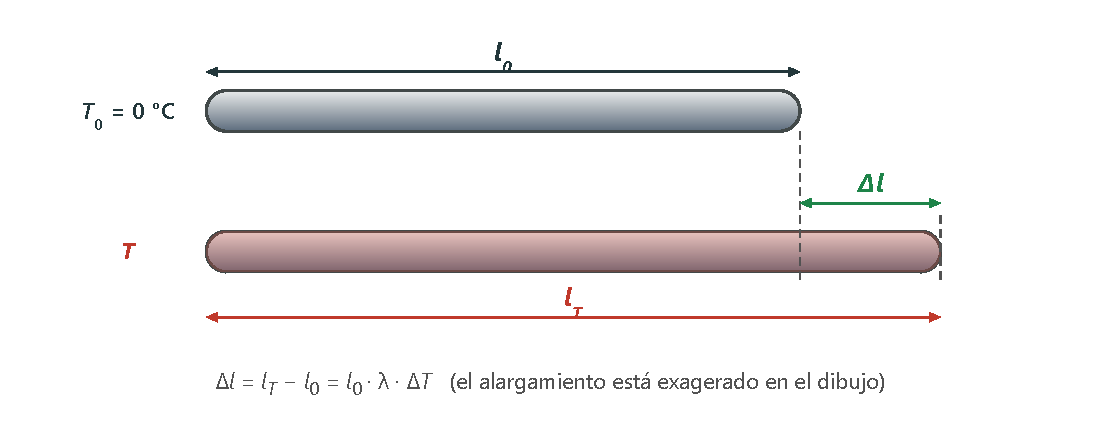
\includegraphics[width=0.65\textwidth]{images/UD13/dilatacion}
    \caption{Dilatación lineal de una barra.}
    \label{fig:ud13-dilatacion}
\end{figure}

La dilatación se tiene en cuenta en ingeniería: los puentes y las vías tienen \textbf{juntas de dilatación}, y los cables del
tendido eléctrico se cuelgan algo flojos para que no se rompan al contraerse en invierno. Los termostatos de muchos aparatos
usan una \textbf{lámina bimetálica}, dos metales soldados que se dilatan distinto: al calentarse se curva y abre o cierra un
circuito (figura~\ref{fig:ud13-bimetal}).

\begin{figure}[H]
    \centering
    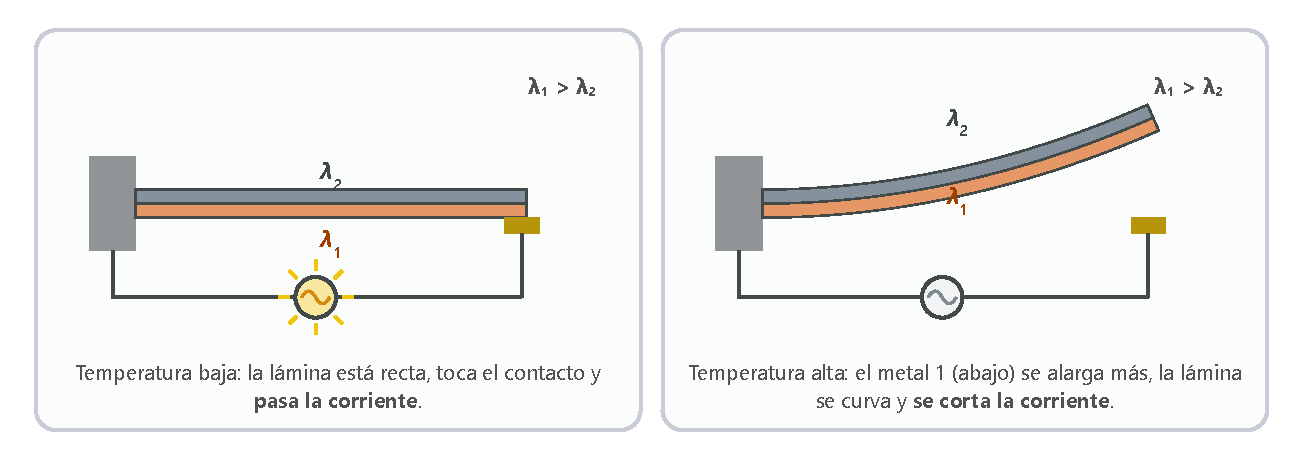
\includegraphics[width=0.85\textwidth]{images/UD13/bimetal}
    \caption{Termostato de lámina bimetálica.}
    \label{fig:ud13-bimetal}
\end{figure}

\begin{example}
    \textbf{Juntas en las vías.} Un raíl de acero mide \qty{25}{\m} a \qty{10}{\degreeCelsius}. ¿Cuánto se alarga un día de verano en
    que alcanza \qty{45}{\degreeCelsius}? \(\lambda_{\text{acero}} = \qty{1.2e-5}{\per\kelvin}\).

    \textbf{Solución.} \(\Delta L = L_0\,\lambda\,\Delta T = 25 \cdot \num{1.2e-5} \cdot (45 - 10) = \qty{1.05e-2}{\m} =
    \qty{10.5}{\mm}\). Por eso se deja un hueco de algo más de un centímetro entre raíles.
\end{example}

\begin{exercise}
    Una barra de aluminio mide \qty{3}{\m} a \qty{20}{\degreeCelsius}. ¿Cuánto se alarga si se calienta hasta \qty{180}{\degreeCelsius}?
    \(\lambda = \qty{2.4e-5}{\per\kelvin}\).
    \begin{solu}
        \(\Delta L = 3 \cdot \num{2.4e-5} \cdot 160 = \qty{1.15e-2}{\m} = \textcolor{red}{\qty{11.5}{\mm}}\).
    \end{solu}
\end{exercise}

%========================================================================================
\section{Intercambio de energía en forma de trabajo}\label{sec:ud13-trabajo}
%========================================================================================

El \textbf{trabajo termodinámico} es la energía que intercambian el sistema y el entorno sin que intervenga una diferencia de
temperatura. Suele ir asociado a una fuerza que produce un desplazamiento en el sistema: en un gas, al cambiar su volumen.

\subsection{Trabajo de expansión o compresión de un gas}

Imaginemos un gas encerrado en un cilindro con un émbolo de superficie \(S\) que puede moverse sin rozamiento, sometido a una
presión exterior constante \(p\) (figura~\ref{fig:ud13-embolo}). Si calentamos el gas, sus partículas chocan con más energía
contra el émbolo, lo empujan y el gas se expande: el émbolo sube \(\Delta h\) y el volumen aumenta \(\Delta V = S\,\Delta h\).

\begin{figure}[H]
    \centering
    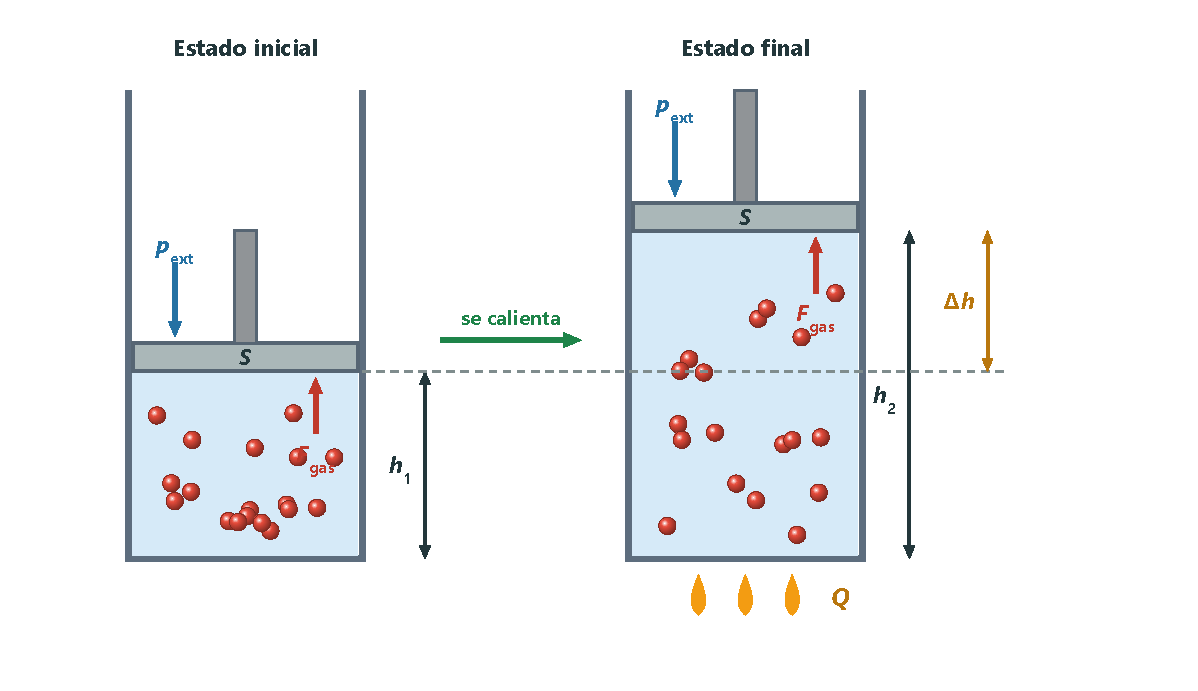
\includegraphics[width=0.7\textwidth]{images/UD13/expansion_embolo}
    \caption{Expansión de un gas a presión constante.}
    \label{fig:ud13-embolo}
\end{figure}

La fuerza que vence el gas es \(F = p\,S\), y con nuestro criterio de signos el trabajo de expansión es negativo (el sistema
pierde energía):
\[ W = -F\,\Delta h = -p\,S\,\Delta h = -p\,\Delta V = -p\,(V_f - V_i) \]

\begin{table}[H]
    \centering
    \caption{Signo del trabajo de un gas}
    \vspace{-5pt}
    \begin{tabular}{@{}lcL{9.5cm}@{}}
        \toprule
        \textbf{Proceso} & \textbf{Signo} & \textbf{Descripción} \\
        \midrule
        Expansión & \(W < 0\) & \(\Delta V > 0\): el gas realiza trabajo sobre el entorno y pierde energía. \\[3pt]
        Compresión & \(W > 0\) & \(\Delta V < 0\): el entorno realiza trabajo sobre el gas y le comunica energía. \\[3pt]
        Volumen constante & \(W = 0\) & \(\Delta V = 0\): no hay trabajo de expansión ni de compresión. \\
        \bottomrule
    \end{tabular}
    \label{tab:ud13-signo-trabajo}
\end{table}

\begin{remark}
    Para que el trabajo salga en julios, la presión debe ir en pascales y el volumen en metros cúbicos:
    \(\qty{1}{\litre} = \qty{e-3}{\m\cubed}\) y \(\qty{1}{\cm\cubed} = \qty{e-6}{\m\cubed}\). También es útil saber que
    \(\qty{1}{\atm\litre} = \qty{101.3}{\joule}\).
\end{remark}

\begin{example}
    \textbf{Expansión contra la presión exterior.} Un gas encerrado en un cilindro de paredes adiabáticas con un émbolo móvil ocupa
    \qty{3}{\litre}. Se expande hasta \qty{8}{\litre} contra una presión exterior constante de \qty{150}{\kilo\pascal}. ¿Qué trabajo
    se realiza?

    \textbf{Solución.} \(W = -p\,(V_f - V_i) = -\num{1.5e5} \cdot (8 - 3) \cdot \num{e-3} = \qty{-750}{\joule}\). Es negativo porque
    el gas hace trabajo sobre el entorno.
\end{example}

\begin{exercise}
    Si el gas del ejemplo anterior se comprimiera de \qty{6}{\litre} a \qty{2}{\litre} a una presión de \qty{120}{\kilo\pascal}, ¿qué
    trabajo se realizaría? ¿Y si el proceso fuera isocórico?
    \begin{solu}
        \(W = -\num{1.2e5} \cdot (2 - 6) \cdot \num{e-3} = \textcolor{red}{\qty{+480}{\joule}}\). En un proceso isocórico,
        \(\Delta V = 0\) y \(W = \textcolor{red}{0}\).
    \end{solu}
\end{exercise}

\begin{exercise}
    Calcula el trabajo realizado al comprimir un gas desde \qty{800}{\cm\cubed} hasta \qty{300}{\cm\cubed} con una presión exterior
    de \qty{250}{\kilo\pascal}.
    \begin{solu}
        \(W = -\num{2.5e5} \cdot (300 - 800) \cdot \num{e-6} = \textcolor{red}{\qty{+125}{\joule}}\).
    \end{solu}
\end{exercise}

\subsection{Diagramas \texorpdfstring{\(p\)-\(V\)}{p-V}}

Los procesos de un gas se representan en un diagrama \(p\)-\(V\), con el volumen en abscisas y la presión en ordenadas. En un
proceso isobárico, la gráfica es una recta horizontal y \(|W| = p\,\Delta V\) es el área del rectángulo bajo ella. Esta idea se
generaliza a cualquier proceso:

\begin{definition}[Interpretación gráfica del trabajo]
    El \textbf{valor absoluto del trabajo} intercambiado en un proceso es el \textbf{área} comprendida entre la gráfica \(p = p(V)\) y
    el eje de abscisas, entre \(V_i\) y \(V_f\). El signo es negativo si el volumen aumenta y positivo si disminuye.
\end{definition}

\begin{figure}[H]
    \centering
    \begin{tikzpicture}
        \begin{axis}[grafica, width=0.36\linewidth, height=4.4cm, xlabel={\(V\)}, ylabel={\(p\)}, xmin=0, xmax=6, ymin=0, ymax=5,
            xtick={1.2,4.8}, xticklabels={\(V_A\),\(V_B\)}, ytick=\empty, title={\small Isobárico}]
            \addplot[fill=ocre!25, draw=none] coordinates {(1.2,0) (1.2,3) (4.8,3) (4.8,0)} \closedcycle;
            \addplot[very thick, ocre, -latex] coordinates {(1.2,3) (4.8,3)};
            \node[font=\small] at (axis cs:3,1.5) {\(W = -p\,\Delta V\)};
            \node[font=\small, anchor=south] at (axis cs:1.2,3) {A};
            \node[font=\small, anchor=south] at (axis cs:4.8,3) {B};
        \end{axis}
    \end{tikzpicture}\hfill
    \begin{tikzpicture}
        \begin{axis}[grafica, width=0.36\linewidth, height=4.4cm, xlabel={\(V\)}, ylabel={\(p\)}, xmin=0, xmax=6, ymin=0, ymax=5,
            xtick={1.2,4.8}, xticklabels={\(V_A\),\(V_B\)}, ytick=\empty, title={\small Isotérmico}]
            \addplot[fill=ocre!25, draw=none, domain=1.2:4.8] {5/x} \closedcycle;
            \addplot[thick, gray, dashed, domain=1.05:5.8] {5/x};
            \addplot[very thick, ocre, domain=1.2:4.8] {5/x};
            \node[font=\small] at (axis cs:2.9,0.8) {\(W\)};
            \node[font=\small, anchor=south west] at (axis cs:1.2,4.17) {A};
            \node[font=\small, anchor=south west] at (axis cs:4.8,1.04) {B};
        \end{axis}
    \end{tikzpicture}\hfill
    \begin{tikzpicture}
        \begin{axis}[grafica, width=0.36\linewidth, height=4.4cm, xlabel={\(V\)}, ylabel={\(p\)}, xmin=0, xmax=6, ymin=0, ymax=5,
            xtick={3}, xticklabels={\(V\)}, ytick=\empty, title={\small Isocórico}]
            \addplot[very thick, ocre, -latex] coordinates {(3,1.2) (3,4)};
            \addplot[thin, gray, dashed] coordinates {(0,1.2) (3,1.2)};
            \addplot[thin, gray, dashed] coordinates {(0,4) (3,4)};
            \node[font=\small, anchor=west] at (axis cs:3,1.2) {A};
            \node[font=\small, anchor=west] at (axis cs:3,4) {B};
            \node[font=\small] at (axis cs:4.5,2.6) {\(W = 0\)};
        \end{axis}
    \end{tikzpicture}
    \caption{Trabajo en los diagramas \(p\)-\(V\): es el área bajo la gráfica.}
    \label{fig:ud13-diagramas}
\end{figure}

\begin{itemize}
    \item \textbf{Isobárico}: recta horizontal; \(W = -p\,(V_B - V_A)\).
    \item \textbf{Isotérmico}: según la ley de Boyle, \(p = n\,R\,T/V\), la gráfica es una hipérbola. El cálculo del área (con una
    integral, que estudiarás en Matemáticas) da:
    \[ W = -n\,R\,T \ln\frac{V_B}{V_A} \]
    \item \textbf{Isocórico}: recta vertical; el área es nula y \(W = 0\).
\end{itemize}

Si el sistema recorre un \textbf{ciclo} (vuelve al estado inicial), el trabajo total es el \textbf{área encerrada} por el ciclo:
es negativo (el gas hace trabajo neto) si el ciclo se recorre en sentido horario, y positivo si se recorre en sentido antihorario.

\begin{example}
    \textbf{Trabajo en un ciclo.} Un gas recorre el ciclo de la figura~\ref{fig:ud13-ciclo}: 1 (\qty{1.5}{\litre},
    \qty{250}{\kilo\pascal}) \(\rightarrow\) 2 (\qty{5.5}{\litre}, \qty{250}{\kilo\pascal}) \(\rightarrow\) 3 (\qty{5.5}{\litre},
    \qty{100}{\kilo\pascal}) \(\rightarrow\) 4 (\qty{1.5}{\litre}, \qty{100}{\kilo\pascal}) \(\rightarrow\) 1. Calcula el trabajo en
    cada tramo y en el ciclo completo.

    \textbf{Solución.} Tramos isocóricos (2 \(\rightarrow\) 3 y 4 \(\rightarrow\) 1): \(W = 0\). Tramos isobáricos:
    \begin{gather*}
        W_{1\to2} = -\num{2.5e5} \cdot (\num{5.5} - \num{1.5}) \cdot \num{e-3} = \qty{-1000}{\joule} \\
        W_{3\to4} = -\num{1.0e5} \cdot (\num{1.5} - \num{5.5}) \cdot \num{e-3} = \qty{+400}{\joule}
    \end{gather*}
    \(W_{\text{ciclo}} = -1000 + 0 + 400 + 0 = \qty{-600}{\joule}\). Coincide con el área del rectángulo,
    \((250 - 100)\,\unit{\kilo\pascal} \cdot \qty{4}{\litre} = \qty{600}{\joule}\), con signo negativo porque se recorre en sentido
    horario: el gas realiza trabajo neto sobre el entorno.
\end{example}

\begin{figure}[H]
    \centering
    \begin{tikzpicture}
        \begin{axis}[grafica, width=0.5\linewidth, height=5cm, xlabel={\(V\) (L)}, ylabel={\(p\) (kPa)}, xmin=0, xmax=7, ymin=0,
            ymax=300, xtick={1.5,5.5}, ytick={100,250}]
            \addplot[fill=ocre!20, draw=none] coordinates {(1.5,100) (1.5,250) (5.5,250) (5.5,100)} -- cycle;
            \addplot[very thick, ocre, -latex] coordinates {(1.5,250) (3.6,250)};
            \addplot[very thick, ocre, -latex] coordinates {(3.5,250) (5.5,250) (5.5,170)};
            \addplot[very thick, ocre, -latex] coordinates {(5.5,180) (5.5,100) (3.4,100)};
            \addplot[very thick, ocre, -latex] coordinates {(3.5,100) (1.5,100) (1.5,180)};
            \addplot[very thick, ocre] coordinates {(1.5,175) (1.5,250)};
            \node[font=\small, anchor=south east] at (axis cs:1.5,250) {1};
            \node[font=\small, anchor=south west] at (axis cs:5.5,250) {2};
            \node[font=\small, anchor=north west] at (axis cs:5.5,100) {3};
            \node[font=\small, anchor=north east] at (axis cs:1.5,100) {4};
        \end{axis}
    \end{tikzpicture}
    \caption{Ciclo rectangular en un diagrama \(p\)-\(V\).}
    \label{fig:ud13-ciclo}
\end{figure}

\begin{example}
    \textbf{Expansión isotérmica.} \qty{0.20}{\mol} de un gas ideal a \qty{27}{\degreeCelsius} se expanden de forma isotérmica desde
    \qty{2.0}{\litre} hasta \qty{5.0}{\litre}. ¿Qué trabajo se realiza?

    \textbf{Solución.} \(T = \qty{300}{\kelvin}\):
    \(W = -n\,R\,T\ln\dfrac{V_B}{V_A} = -\num{0.20} \cdot \num{8.31} \cdot 300 \cdot \ln\dfrac{5}{2} = \qty{-457}{\joule}\).
\end{example}

\begin{exercise}
    Representa en un diagrama \(p\)-\(V\) un proceso isocórico, uno isobárico y uno isotérmico, e indica en cuál de ellos es nulo el
    trabajo.
    \begin{solu}
        Isocórico: recta vertical; isobárico: recta horizontal; isotérmico: rama de hipérbola. El trabajo es nulo en el
        \textcolor{red}{isocórico}.
    \end{solu}
\end{exercise}

\begin{exercise}
    Un gas recorre el ciclo triangular 1 (\qty{2}{\litre}, \qty{300}{\kilo\pascal}) \(\rightarrow\) 2 (\qty{8}{\litre},
    \qty{100}{\kilo\pascal}) en línea recta \(\rightarrow\) 3 (\qty{2}{\litre}, \qty{100}{\kilo\pascal}) \(\rightarrow\) 1. Calcula el
    trabajo en cada tramo y en el ciclo.
    \begin{solu}
        \(W_{1\to2} = -\dfrac{300 + 100}{2}\,\unit{\kilo\pascal} \cdot \qty{6}{\litre} = \textcolor{red}{\qty{-1200}{\joule}}\) (área del
        trapecio); \(W_{2\to3} = -\num{1e5} \cdot (2 - 8) \cdot \num{e-3} = \textcolor{red}{\qty{+600}{\joule}}\);
        \(W_{3\to1} = \textcolor{red}{0}\). \(W_{\text{ciclo}} = \textcolor{red}{\qty{-600}{\joule}}\) (área del triángulo).
    \end{solu}
\end{exercise}

%========================================================================================
\section{Energía interna y primer principio de la termodinámica}\label{sec:ud13-primer-principio}
%========================================================================================

Las partículas de un sistema tienen energía cinética de traslación, pero también de rotación y de vibración, y energía potencial
debida a las fuerzas entre ellas (figura~\ref{fig:ud13-energia-interna}).

\begin{definition}[Energía interna]
    La \textbf{energía interna} \(U\) de un sistema es la suma de todas las energías de las partículas que lo forman. Es una
    \textbf{función de estado} y se mide en julios.
\end{definition}

\begin{figure}[H]
    \centering
    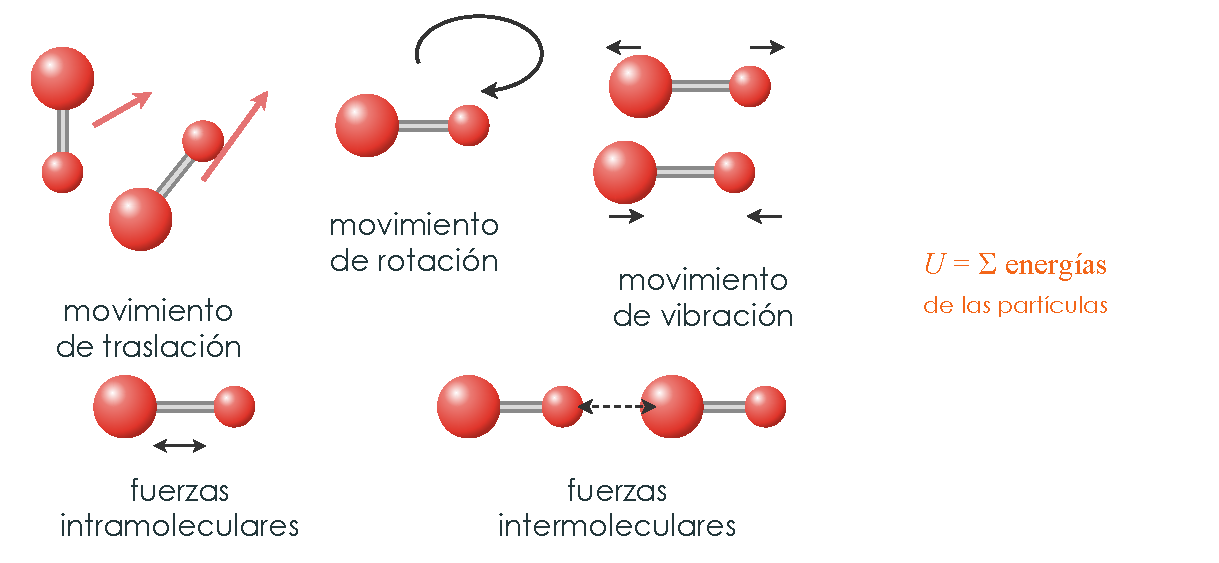
\includegraphics[width=0.7\textwidth]{images/UD13/energia_interna}
    \caption{Contribuciones a la energía interna.}
    \label{fig:ud13-energia-interna}
\end{figure}

No podemos medir la energía de cada partícula, así que no conocemos el valor absoluto de \(U\); pero sí podemos medir su
\textbf{variación}, \(\Delta U\), cuando el sistema pasa de un estado a otro. En un \textbf{gas ideal} no hay fuerzas entre las
partículas y la energía interna depende solo de la temperatura: si \(T\) no cambia, \(U\) tampoco.

\begin{definition}[Primer principio de la termodinámica]
    La variación de la energía interna de un sistema es igual a la suma del calor y del trabajo que intercambia con su entorno:
    \[ \Delta U = Q + W \]
\end{definition}

Es el \textbf{principio de conservación de la energía} aplicado a los sistemas termodinámicos: la energía no se crea ni se
destruye, de modo que si la energía interna de un sistema cambia, es porque ha intercambiado calor o trabajo con el entorno. Lo
enunció \textbf{Rudolf Clausius} en 1850, a partir de los trabajos de Carnot y de Joule.

Con nuestro criterio de signos:
\begin{itemize}
    \item El calor absorbido y el trabajo recibido aumentan \(U\); el calor cedido y el trabajo realizado la disminuyen.
    \item En un \textbf{proceso cíclico}, el sistema vuelve al estado inicial y, como \(U\) es función de estado,
    \(\Delta U = 0\): \(Q = -W\). En un \textbf{sistema aislado}, \(Q = W = 0\) y \(U\) es constante.
\end{itemize}

\begin{table}[H]
    \centering
    \caption{El primer principio en los distintos procesos}
    \vspace{-5pt}
    \begin{tabular}{@{}lcL{7.8cm}@{}}
        \toprule
        \textbf{Proceso} & \textbf{Primer principio} & \textbf{Comentario} \\
        \midrule
        Adiabático & \(\Delta U = W\) & No hay calor; la energía interna cambia solo por el trabajo. En una compresión
        adiabática \(W > 0\) y el gas se calienta. \\[3pt]
        Isocórico & \(\Delta U = Q_V\) & \(W = 0\): todo el calor a volumen constante, \(Q_V\), se invierte en cambiar \(U\). \\[3pt]
        Isobárico & \(\Delta U = Q_p - p\,\Delta V\) & \(Q_p\) es el calor a presión constante. \\[3pt]
        Isotérmico (gas ideal) & \(\Delta U = 0\) & \(T\) no cambia, \(U\) tampoco: \(Q = -W\). \\
        \bottomrule
    \end{tabular}
    \label{tab:ud13-primer-principio}
\end{table}

\begin{remark}
    En química, la mayoría de las reacciones tienen lugar a presión constante. Despejando, \(Q_p = \Delta U + p\,\Delta V =
    \Delta(U + p\,V)\). La magnitud \(H = U + p\,V\) es la \textbf{entalpía}, otra función de estado, y \(Q_p = \Delta H\): es la
    entalpía de reacción que estudiamos en la sección~\ref{sec:ud6-energia}.
\end{remark}

\begin{example}
    \textbf{Calor, trabajo y energía interna.} Calcula la variación de energía interna de un sistema que: a) absorbe \qty{450}{\joule}
    de calor y realiza un trabajo de expansión de \qty{200}{\joule}; b) cede \qty{120}{\joule} de calor y recibe un trabajo de
    compresión de \qty{300}{\joule}.

    \textbf{Solución.} a) \(Q = \qty{+450}{\joule}\), \(W = \qty{-200}{\joule}\): \(\Delta U = 450 - 200 = \qty{+250}{\joule}\).
    b) \(Q = \qty{-120}{\joule}\), \(W = \qty{+300}{\joule}\): \(\Delta U = -120 + 300 = \qty{+180}{\joule}\). En los dos casos la
    energía interna aumenta.
\end{example}

\begin{example}
    \textbf{Expansión a presión constante.} Un gas se expande a una presión constante de \qty{2}{\atm} desde \qty{4}{\litre} hasta
    \qty{10}{\litre}, y absorbe \qty{2.5}{\kilo\joule} de calor. Calcula el trabajo y la variación de energía interna.

    \textbf{Solución.} \(W = -p\,\Delta V = -2 \cdot 101325 \cdot (10 - 4) \cdot \num{e-3} = \qty{-1216}{\joule}\).
    \(\Delta U = Q + W = 2500 - 1216 = \qty{+1284}{\joule}\). Parte del calor se invierte en trabajo y el resto aumenta la energía
    interna del gas (y su temperatura).
\end{example}

\begin{exercise}
    En un proceso isotérmico, un gas ideal libera \qty{500}{\kilo\joule} de calor. ¿Cuánto vale el trabajo? ¿Es de expansión o de
    compresión?
    \begin{solu}
        \(\Delta U = 0 \Rightarrow W = -Q = \textcolor{red}{\qty{+500}{\kilo\joule}}\): es un trabajo de
        \textcolor{red}{compresión} (el entorno hace trabajo sobre el gas).
    \end{solu}
\end{exercise}

\begin{exercise}
    a) ¿Cuál es la variación de energía interna de un sistema al que se transfieren \qty{300}{\calorie} y sobre el que se realiza un
    trabajo de \qty{400}{\joule}? b) La energía interna de un sistema aumenta \qty{500}{\joule} mientras desprende \qty{640}{\joule}
    de calor. ¿Qué trabajo se ha realizado sobre él?
    \begin{solu}
        a) \(\Delta U = 300 \cdot \num{4.18} + 400 = \textcolor{red}{\qty{1654}{\joule}}\). b) \(W = \Delta U - Q = 500 - (-640) =
        \textcolor{red}{\qty{+1140}{\joule}}\).
    \end{solu}
\end{exercise}

\begin{exercise}
    ¿Por qué cuando hace frío nos frotamos las manos para calentarlas? Explícalo con el primer principio.
    \begin{solu}
        Al frotar realizamos \textcolor{red}{trabajo contra el rozamiento} (\(W > 0\) sobre la piel). Como el proceso es rápido,
        apenas hay calor intercambiado y \(\Delta U \approx W > 0\): aumenta la energía interna de la piel y, con ella, su
        temperatura.
    \end{solu}
\end{exercise}

%========================================================================================
\section{Entropía y segundo principio de la termodinámica}\label{sec:ud13-segundo-principio}
%========================================================================================

El trabajo se puede convertir por completo en calor (piensa en los frenos de un coche), pero ¿se puede convertir todo el calor en
trabajo? El primer principio no lo impide, ni explica por qué unos procesos ocurren espontáneamente y sus inversos no: el hierro se
oxida, pero el óxido nunca vuelve a ser hierro por sí solo; el café caliente se enfría, pero jamás se calienta solo a costa del
aire de la habitación. Para responder necesitamos una nueva magnitud.

\subsection{La entropía}

\begin{definition}[Entropía]
    La \textbf{entropía} \(S\) es una función de estado extensiva que mide el \textbf{grado de desorden} molecular de un sistema
    (más exactamente, el número de formas microscópicas en que puede organizarse). Se mide en \unit{\joule\per\kelvin}.
\end{definition}

\begin{itemize}
    \item Para una misma sustancia, \(S_{\text{gas}} \gg S_{\text{líquido}} > S_{\text{sólido}}\). La entropía aumenta al fundir,
    vaporizar, disolver, mezclar o calentar.
    \item En una reacción química, la entropía suele aumentar si aumenta el número de moles de gas.
    \item \textbf{Clausius} (1865) relacionó la variación de entropía con el calor absorbido a una temperatura \(T\): en un proceso
    reversible \(\Delta S = Q/T\), y en uno irreversible \(\Delta S > Q/T\).
\end{itemize}

\begin{example}
    \textbf{La entropía de un cubito.} ¿Cuánto aumenta la entropía de \qty{100}{\g} de hielo al fundirse a \qty{0}{\degreeCelsius}?
    \(L_f = \qty{3.34e5}{\joule\per\kg}\).

    \textbf{Solución.} La fusión es reversible e isotérmica: \(Q = m\,L_f = \num{0.1} \cdot \num{3.34e5} = \qty{33400}{\joule}\) y
    \(\Delta S = \dfrac{Q}{T} = \dfrac{33400}{\num{273.15}} = \qty{+122}{\joule\per\kelvin}\). Aumenta, porque el líquido está más
    desordenado que el sólido.
\end{example}

\subsection{El segundo principio}

\begin{definition}[Segundo principio de la termodinámica]
    En todo proceso espontáneo, la entropía del universo aumenta:
    \[ \Delta S_{\text{universo}} = \Delta S_{\text{sistema}} + \Delta S_{\text{entorno}} \geq 0 \]
    La igualdad solo se cumple en los procesos reversibles, que son ideales.
\end{definition}

La entropía de un sistema \textbf{puede disminuir} (al congelar agua o al ordenar una habitación), pero a costa de que aumente más
la del entorno. Consecuencias:
\begin{itemize}
    \item Marca la \textbf{flecha del tiempo}: los procesos naturales transcurren en el sentido en que aumenta la entropía del
    universo; nunca vemos un vaso roto recomponerse solo.
    \item El calor pasa espontáneamente del cuerpo caliente al frío, y nunca al revés (enunciado de Clausius).
    \item La energía se \textbf{degrada}: aunque la energía total del universo es constante, cada vez una parte mayor está en
    forma de calor a baja temperatura, del que no se puede obtener trabajo útil. Por eso hablamos de «crisis energética» aunque la
    energía se conserve: lo que se agota es la energía de calidad, la que podemos aprovechar.
\end{itemize}

\subsection{Máquinas térmicas}

\begin{definition}[Máquina térmica]
    Es un dispositivo que transforma parte del calor en trabajo mediante un \textbf{proceso cíclico} (\(\Delta U = 0\)). Toma un
    calor \(Q_1\) de un \textbf{foco caliente} a temperatura \(T_1\), realiza un trabajo \(W\) y cede un calor \(Q_2\) a un
    \textbf{foco frío} a temperatura \(T_2\) (figura~\ref{fig:ud13-maquina}). En valor absoluto: \(|Q_1| = |W| + |Q_2|\).
\end{definition}

\begin{figure}[H]
    \centering
    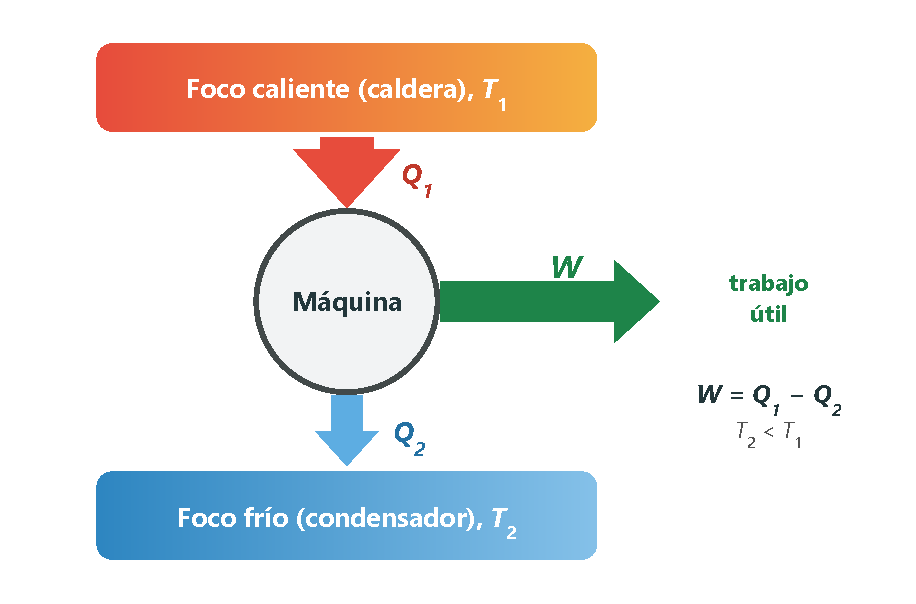
\includegraphics[width=0.6\textwidth]{images/UD13/maquina_termica}
    \caption{Esquema de una máquina térmica.}
    \label{fig:ud13-maquina}
\end{figure}

El \textbf{rendimiento} es la fracción del calor absorbido que se convierte en trabajo:
\[ \eta = \frac{|W|}{|Q_1|} = \frac{|Q_1| - |Q_2|}{|Q_1|} \]
Una consecuencia del segundo principio es que siempre \(\eta < 1\): \textbf{no es posible transformar íntegramente en trabajo el
calor absorbido} (enunciado de Kelvin-Planck). Carnot demostró que ninguna máquina que trabaje entre dos focos puede superar el
rendimiento de una máquina ideal reversible, la \textbf{máquina de Carnot}:
\[ \eta_{\text{máx}} = 1 - \frac{T_2}{T_1} \qquad \text{(temperaturas en kelvin)} \]

Son máquinas térmicas la máquina de vapor, las turbinas de las centrales térmicas y los \textbf{motores de combustión}, como el
motor de cuatro tiempos de los coches (figura~\ref{fig:ud13-motor}). Los \textbf{frigoríficos} y las \textbf{bombas de calor} son
máquinas térmicas que funcionan al revés: con un trabajo, extraen calor de un foco frío y lo ceden a uno caliente.

\begin{figure}[H]
    \centering
    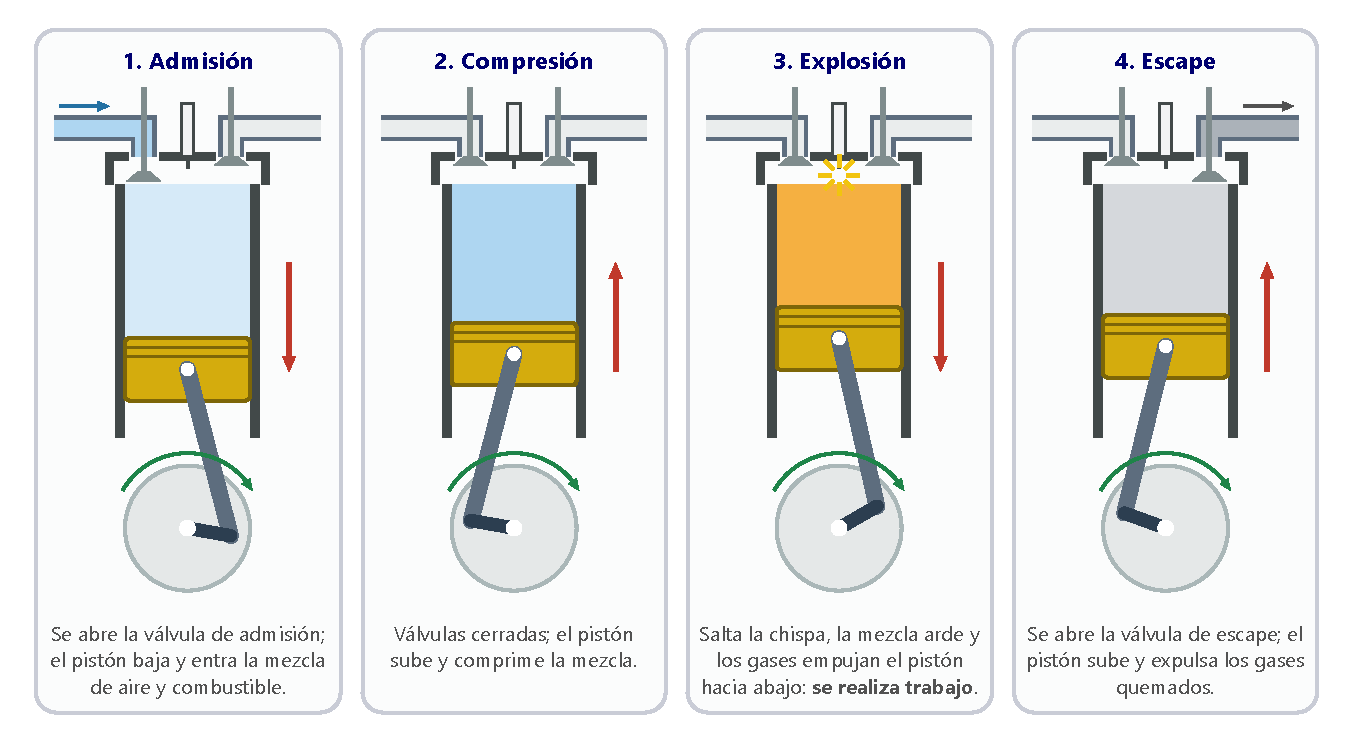
\includegraphics[width=\textwidth]{images/UD13/motor_cuatro_tiempos}
    \caption{Los cuatro tiempos de un motor de gasolina.}
    \label{fig:ud13-motor}
\end{figure}

\begin{example}
    \textbf{Rendimiento de un motor.} Un motor térmico realiza un trabajo de \qty{160}{\joule} en cada ciclo, y absorbe
    \qty{130}{\calorie} del foco caliente. a) Calcula su rendimiento. b) ¿Qué calor cede al foco frío en cada ciclo? c) Si trabaja
    entre \qty{500}{\degreeCelsius} y \qty{30}{\degreeCelsius}, ¿cuál sería su rendimiento máximo?

    \textbf{Solución.} a) \(Q_1 = 130 \cdot \num{4.18} = \qty{543.4}{\joule}\);
    \(\eta = \dfrac{160}{\num{543.4}} = \num{0.294}\), es decir, un \qty{29.4}{\percent}.

    b) \(|Q_2| = |Q_1| - |W| = \num{543.4} - 160 = \qty{383}{\joule}\).

    c) \(\eta_{\text{máx}} = 1 - \dfrac{303}{773} = \num{0.608}\), un \qty{60.8}{\percent}. El motor real queda lejos del ideal por
    el rozamiento, las pérdidas de calor y la irreversibilidad de la combustión.
\end{example}

\begin{exercise}
    Indica razonadamente si aumenta o disminuye la entropía del sistema en cada caso: a) se funde un cubito de hielo; b) ordenas tu
    cuarto; c) calientas una barra de hierro; d) congelas un caldo; e) preparas un café con leche; f) arde una hoguera.
    \begin{solu}
        Aumenta en \textcolor{red}{a, c, e y f} (más desorden: fusión, mayor agitación, mezcla, formación de gases). Disminuye en
        \textcolor{red}{b y d} (más orden); en b, la entropía del universo aumenta igualmente por el calor que desprende nuestro
        cuerpo al trabajar.
    \end{solu}
\end{exercise}

\begin{exercise}
    Pronostica cómo cambia la entropía en estas reacciones: a) \ch{2 H2O2(aq) -> 2 H2O(l) + O2(g)}; b) \ch{N2(g) + 3 H2(g) -> 2
    NH3(g)}; c) \ch{CaCO3(s) -> CaO(s) + CO2(g)}; d) \ch{H2O(g) -> H2O(l)}.
    \begin{solu}
        a) \textcolor{red}{Aumenta} (se forma un gas). b) \textcolor{red}{Disminuye} (de 4 a 2 moles de gas). c)
        \textcolor{red}{Aumenta} (se forma un gas a partir de un sólido). d) \textcolor{red}{Disminuye} (condensación).
    \end{solu}
\end{exercise}

\begin{exercise}
    Una máquina térmica absorbe \qty{2000}{\joule} del foco caliente y cede \qty{1400}{\joule} al foco frío en cada ciclo. Calcula el
    trabajo que realiza y su rendimiento.
    \begin{solu}
        \(|W| = 2000 - 1400 = \textcolor{red}{\qty{600}{\joule}}\); \(\eta = \dfrac{600}{2000} = \textcolor{red}{\qty{30}{\percent}}\).
    \end{solu}
\end{exercise}

%========================================================================================
\section{Física en la vida: energía solar fotovoltaica y termodinámica}\label{sec:ud13-solar}
%========================================================================================

España recibe entre \num{2500} y \num{3000} horas de sol al año, así que la \textbf{energía solar} es una alternativa limpia y
rentable a los combustibles fósiles. Hay dos formas principales de aprovecharla en una vivienda.

Los \textbf{paneles fotovoltaicos} transforman directamente la luz en electricidad. Están formados por células de silicio, un
semiconductor que absorbe los fotones y libera electrones, lo que produce una corriente continua; un \textbf{inversor} la convierte
en alterna para usarla en casa. Necesitan un mínimo de radiación solar para funcionar y duran entre 25 y 30 años.

Los \textbf{paneles solares térmicos} calientan un líquido que circula por su interior y se usan para la calefacción y el agua
caliente sanitaria (ACS). Una variante son los \textbf{paneles solares termodinámicos}: en realidad son una \textbf{bomba de calor}.
Por ellos circula un líquido refrigerante que hierve a muy baja temperatura y se evapora absorbiendo calor del ambiente, incluso de
noche, con lluvia o a temperaturas por debajo de cero. Un compresor aumenta la presión del gas, y con ella su temperatura; después
el gas se condensa en un intercambiador y cede su calor al agua de un depósito aislado. Como en un frigorífico, con un pequeño
trabajo eléctrico se traslada calor de un foco frío (el aire exterior) a uno caliente (el agua): cada kilovatio hora eléctrico puede
llevar al agua tres o cuatro kilovatios hora de calor. También se investiga en \textbf{paneles híbridos}, que generan a la vez
electricidad y agua caliente; además, al refrigerar las células, mejoran su rendimiento eléctrico.

\begin{exercise}
    a) ¿Qué transformaciones de energía tienen lugar en un panel fotovoltaico y en un panel termodinámico? b) Un panel termodinámico
    entrega \qty{3.5}{\kilo\watt\hour} de calor al agua por cada \qty{1}{\kilo\watt\hour} eléctrico que consume el compresor. ¿Viola
    esto el primer principio? ¿De dónde sale el resto de la energía? c) Investigad qué es la energía \textbf{agrovoltaica} y por qué
    interesa en el sector agrícola.
    \begin{solu}
        a) Fotovoltaico: \textcolor{red}{radiante \(\rightarrow\) eléctrica}. Termodinámico: \textcolor{red}{eléctrica \(\rightarrow\)
        trabajo del compresor}, y el calor del ambiente pasa al agua. b) \textcolor{red}{No}: los \qty{2.5}{\kilo\watt\hour}
        restantes son \textcolor{red}{calor extraído del aire exterior}; el compresor solo lo «bombea» del foco frío al caliente.
        c) \textcolor{red}{Respuesta abierta} (placas solares sobre cultivos o pastos: se comparte el terreno, se da sombra y se
        reduce la evaporación del agua).
    \end{solu}
\end{exercise}

%========================================================================================
\section{Prácticas}\label{sec:ud13-practicas}
%========================================================================================

\subsection{Una nube en una botella}

\noindent\begin{minipage}[t]{0.48\textwidth}
    \textbf{Objetivo}
    \begin{itemize}
        \item Comprobar que una expansión casi adiabática enfría un gas y relacionarlo con el primer principio y con la formación de
        las nubes.
    \end{itemize}
\end{minipage}\hfill
\begin{minipage}[t]{0.48\textwidth}
    \textbf{Material}
    \begin{itemize}
        \item Una botella de plástico de \qty{2}{\litre} con tapón, un poco de agua tibia, una cerilla (o alcohol de farmacia) y,
        si se dispone de ella, una bomba de bicicleta con un tapón perforado y una válvula.
    \end{itemize}
\end{minipage}

\begin{figure}[H]
    \centering
    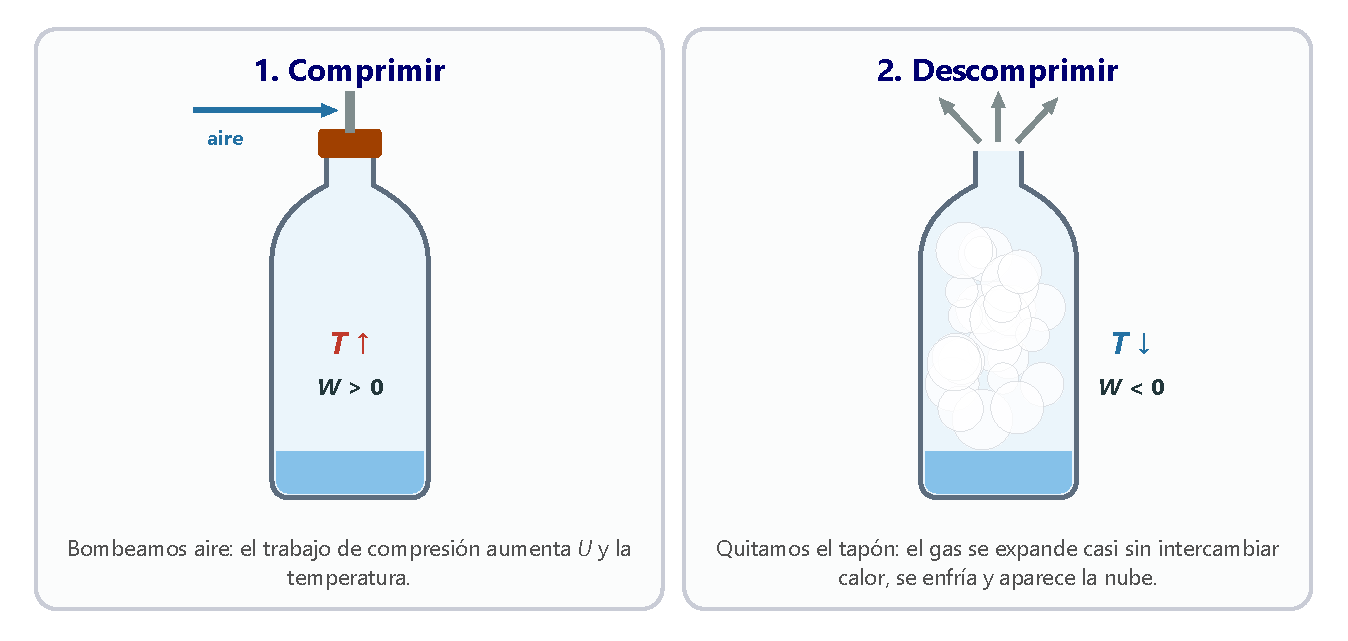
\includegraphics[width=0.75\textwidth]{images/UD13/practica_nube}
    \caption{Al descomprimir el aire de la botella, se enfría y se forma una nube.}
    \label{fig:ud13-nube}
\end{figure}

\textbf{Procedimiento}
\begin{enumerate}[label=\numberballgreen]
    \item Echa un dedo de agua tibia en la botella y agítala para que el aire se cargue de vapor. Vacía el agua.
    \item Enciende una cerilla, apágala y mete el humo en la botella (las partículas de humo sirven de núcleos de condensación,
    como el polvo en la atmósfera). Tapa la botella. Con la supervisión del profesor, se puede usar en su lugar unas gotas de alcohol.
    \item Comprime el aire: aprieta la botella con fuerza unos segundos, o bombea aire con la bomba de bicicleta.
    \item Suelta la botella de golpe (o quita el tapón): en el interior aparece una nube. Si vuelves a apretar, desaparece.
\end{enumerate}

\begin{exercise}
    a) Aplica el primer principio a la compresión y a la expansión del aire de la botella. ¿Por qué podemos considerar que los
    procesos son adiabáticos? b) ¿Por qué aparece la nube? c) Relaciona la experiencia con la formación de las nubes al ascender el
    aire en la atmósfera.
    \begin{solu}
        a) Son tan rápidos que \textcolor{red}{no da tiempo a intercambiar calor}: \(Q \approx 0\) y \(\Delta U = W\). Al
        comprimir, \(W > 0\): \(U\) y la temperatura aumentan. Al expandirse, \(W < 0\): \textcolor{red}{\(U\) y la temperatura
        disminuyen}. b) Al enfriarse, el aire no puede contener tanto vapor y este \textcolor{red}{se condensa} en gotitas sobre las
        partículas de humo. c) El aire que asciende encuentra \textcolor{red}{menor presión, se expande casi adiabáticamente y se
        enfría} (unos \qty{10}{\degreeCelsius} por kilómetro si está seco: es el gradiente adiabático); al llegar al punto de rocío, el
        vapor se condensa y se forma la nube.
    \end{solu}
\end{exercise}

\subsection{Calor específico de un metal}

\noindent\begin{minipage}[t]{0.48\textwidth}
    \textbf{Objetivo}
    \begin{itemize}
        \item Determinar el calor específico de un metal mediante un calorímetro e identificar el metal.
    \end{itemize}
\end{minipage}\hfill
\begin{minipage}[t]{0.48\textwidth}
    \textbf{Material}
    \begin{itemize}
        \item Un calorímetro (o un vaso de poliestireno con tapa), un termómetro, una balanza, un vaso de precipitados, un hornillo, hilo y una
        pieza metálica de unos \qty{150}{\g}.
    \end{itemize}
\end{minipage}

\begin{figure}[H]
    \centering
    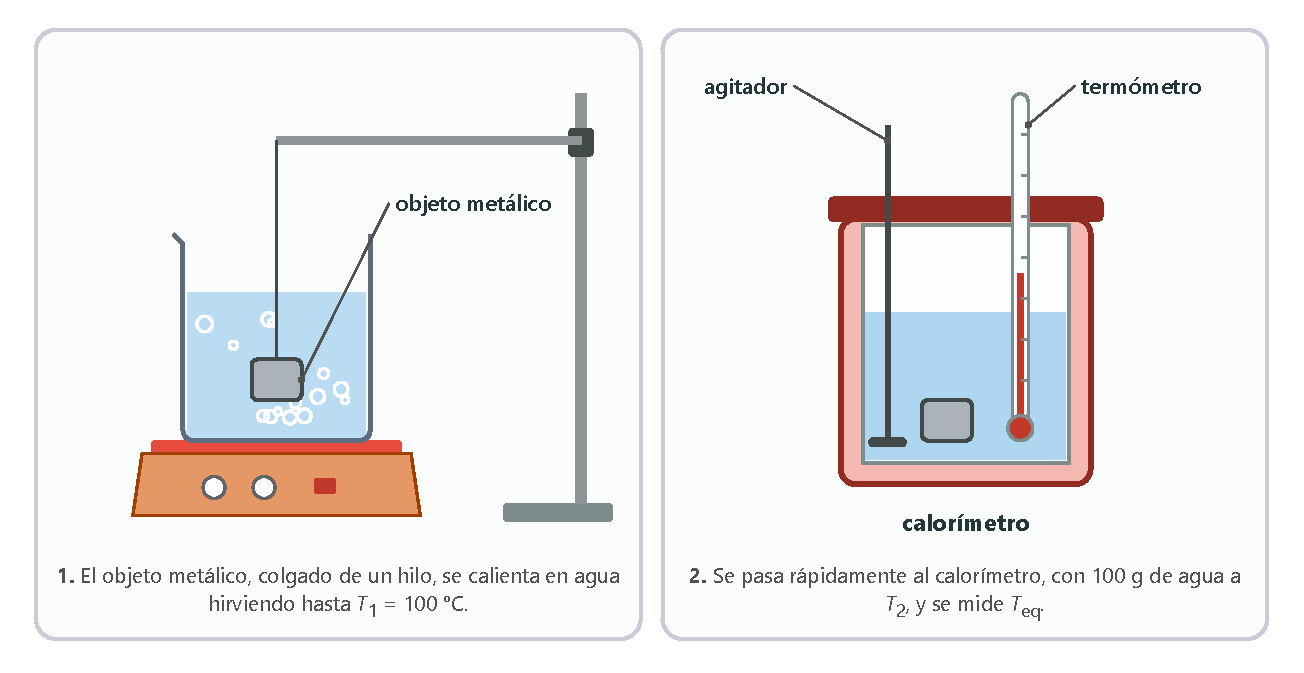
\includegraphics[width=0.75\textwidth]{images/UD13/practica_calor_especifico}
    \caption{Medida del calor específico de un metal.}
    \label{fig:ud13-practica-ce}
\end{figure}

\textbf{Procedimiento}
\begin{enumerate}[label=\numberballgreen]
    \item Pesa la pieza metálica (\(m_1\)), átala con un hilo y sumérgela en agua hirviendo varios minutos: su temperatura será
    \(T_1 = \qty{100}{\degreeCelsius}\).
    \item Echa en el calorímetro una masa conocida de agua (\(m_2\), por ejemplo \qty{200}{\g}) y mide su temperatura, \(T_2\).
    \item Pasa rápidamente la pieza al calorímetro, tápalo, agita y anota la temperatura máxima que alcanza: es \(T_{eq}\).
    \item Con el balance \(m_1\,c_1\,(T_{eq} - T_1) + m_2\,c_{\text{agua}}\,(T_{eq} - T_2) = 0\), calcula \(c_1\) y compáralo con la
    tabla~\ref{tab:ud13-calor-especifico}.
\end{enumerate}

\begin{exercise}
    En la práctica, una pieza de \qty{150}{\g} a \qty{100}{\degreeCelsius} se introduce en \qty{200}{\g} de agua a \qty{20}{\degreeCelsius},
    y el equilibrio se alcanza a \qty{25.2}{\degreeCelsius}. a) Calcula el calor específico del metal. ¿De qué metal se trata? b) ¿El
    valor obtenido será algo mayor o algo menor que el real si el calorímetro pierde calor? ¿Por qué?
    \begin{solu}
        a) \(c_1 = \dfrac{m_2\,c_{\text{agua}}\,(T_{eq} - T_2)}{m_1\,(T_1 - T_{eq})} = \dfrac{\num{0.2} \cdot 4180 \cdot \num{5.2}}{\num{0.15}
        \cdot \num{74.8}} = \textcolor{red}{\qty{387}{\joule\per\kg\per\kelvin}}\): es \textcolor{red}{cobre}. b)
        \textcolor{red}{Menor}: parte del calor del metal se pierde, el agua se calienta menos de lo que debería y parece que el metal
        cedió menos energía.
    \end{solu}
\end{exercise}

%========================================================================================
\section{Situación de aprendizaje: el deshielo del Ártico (ODS 13 y 14)}\label{sec:ud13-ods}
%========================================================================================

El \textbf{ODS 13} pide adoptar medidas urgentes para combatir el cambio climático, y el \textbf{ODS 14}, conservar los océanos y los
mares. Ambos están relacionados con el calor. En el último siglo, el aumento del efecto invernadero ha elevado la temperatura media
del planeta más de \qty{1}{\degreeCelsius}, y el Ártico se calienta unas tres o cuatro veces más deprisa que el resto del mundo: desde
1979 ha perdido en torno a un tercio de su hielo marino en verano. Una de las causas es la \textbf{amplificación ártica}: el hielo y
la nieve reflejan la mayor parte de la luz solar, pero el agua del mar, más oscura, la absorbe; al fundirse el hielo, el océano
absorbe más radiación, se calienta y funde todavía más hielo.

Las consecuencias no son solo ambientales (subida del nivel del mar, pérdida de hábitats de especies como el oso polar o la
morsa), también económicas y geopolíticas: por ejemplo, se abren nuevas rutas marítimas por el Ártico. Se estima que cada
tonelada de \ch{CO2} emitida provoca la desaparición de unos \qty{3}{\m\squared} de hielo ártico en verano. Por eso es importante
conocer nuestra \textbf{huella de carbono}, la cantidad de gases de efecto invernadero que emitimos con nuestras actividades.

\begin{marker}
    \textbf{Reto:} por grupos, investigad la relación entre el calor, el deshielo y nuestra huella de carbono, y grabad un podcast
    de un máximo de tres minutos para la radio escolar.
\end{marker}

\begin{enumerate}[label=\numberballred]
    \item \textbf{Investigad} cuánto calor hace falta para fundir el hielo (ejercicio siguiente) y por qué el agua del mar
    tarda tanto en enfriarse y en calentarse (su calor específico).
    \item \textbf{Calculad} vuestra huella de carbono con una calculadora en línea (por ejemplo, la del Ministerio para la
    Transición Ecológica) y comparadla con la media española.
    \item \textbf{Proponed} medidas para reducirla a nivel individual y en el centro: transporte, alimentación, calefacción y
    aire acondicionado, consumo eléctrico.
    \item \textbf{Comunicad}: escribid un guion argumentado y grabad el podcast (con Audacity o una aplicación gratuita del móvil).
\end{enumerate}

\begin{exercise}
    a) ¿Qué energía hace falta para fundir \qty{1}{\tonne} de hielo a \qty{0}{\degreeCelsius}? b) ¿Y para fundir un bloque de hielo
    marino de \qty{3}{\m\squared} de superficie y \qty{1.5}{\m} de espesor? Densidad del hielo: \qty{917}{\kg\per\m\cubed}.
    c) ¿Durante cuánto tiempo tendría que funcionar un radiador de \qty{2}{\kilo\watt} para suministrar esa energía?
    \begin{solu}
        a) \(Q = m\,L_f = 1000 \cdot \num{3.34e5} = \textcolor{red}{\qty{3.34e8}{\joule}}\). b) \(m = 917 \cdot 3 \cdot \num{1.5} =
        \qty{4127}{\kg}\); \(Q = \textcolor{red}{\qty{1.38e9}{\joule}}\). c) \(t = \dfrac{\num{1.38e9}}{2000} = \qty{6.9e5}{\s}
        \approx \textcolor{red}{8 días}\).
    \end{solu}
\end{exercise}

    \newpage
    %! Unidad 13 — Termodinámica: ejercicios resueltos, ejercicios finales y autoevaluación
%! Fuente: Fuentes/Fisica/Unidad 13 («Ejercicios resueltos», «Practica y calcula», «Piensa y resuelve»). La fuente no trae
%! olimpiadas ni autoevaluación de este tema: la autoevaluación es propia. Enunciados adaptados con datos cambiados y soluciones
%! rehechas con 1 cal = 4,18 J, R = 8,31 J/(mol·K) y 1 atm = 101 325 Pa.
%! Dificultad: \(\star\) baja, \(\star\star\) media, \(\star\star\star\) alta.

\section{Ejercicios resueltos}\label{sec:ud13-resueltos}

\begin{example}
    \textbf{Los cilindros de una moto.} El motor de una moto de competición tiene 4 cilindros de \qty{250}{\cm\cubed} cada uno. En
    cada ciclo, la mezcla de aire y combustible se comprime hasta ocupar \qty{25}{\cm\cubed}, y se pierden \qty{15}{\joule} de calor
    por cilindro. Suponiendo (para simplificar) que la compresión se produce a una presión constante de \qty{101}{\kilo\pascal},
    calcula: a) el trabajo que hace cada cilindro sobre el gas; b) la variación de energía interna del gas.

    \textbf{Solución.} \textbf{1. Unidades SI}: \(V_i = \qty{2.5e-4}{\m\cubed}\), \(V_f = \qty{2.5e-5}{\m\cubed}\),
    \(p = \qty{1.01e5}{\pascal}\).

    \textbf{2. a)} Es una compresión:
    \(W = -p\,(V_f - V_i) = -\num{1.01e5} \cdot (\num{2.5e-5} - \num{2.5e-4}) = \qty{+22.7}{\joule}\). Es positivo porque el
    entorno (el pistón) hace trabajo sobre el gas.

    \textbf{3. b)} El gas cede calor, \(Q = \qty{-15}{\joule}\):
    \(\Delta U = Q + W = -15 + \num{22.7} = \qty{+7.7}{\joule}\). La energía interna (y la temperatura) de la mezcla aumenta.
\end{example}

\begin{example}
    \textbf{Mezcla de agua con paredes adiabáticas y diatérmanas.} En un recipiente con \qty{1500}{\cm\cubed} de agua a
    \qty{12}{\degreeCelsius} se echan \qty{500}{\cm\cubed} de agua a \qty{72}{\degreeCelsius}. La densidad del agua es
    \qty{1}{\g\per\cm\cubed} y \(c_e = \qty{1}{\calorie\per\g\per\degreeCelsius}\). a) Si las paredes son adiabáticas, ¿cuál es la
    temperatura final? b) ¿Qué calor intercambia cada parte? c) ¿Qué ocurriría si las paredes fueran diatérmanas y el exterior
    estuviera a \qty{22}{\degreeCelsius}?

    \textbf{Solución.} \textbf{1. Masas}: \(m_1 = \qty{1500}{\g}\) (fría) y \(m_2 = \qty{500}{\g}\) (caliente).

    \textbf{2. a)} Con paredes adiabáticas, \(Q_1 + Q_2 = 0\):
    \[ m_1\,c_e\,(T - T_1) + m_2\,c_e\,(T - T_2) = 0 \Rightarrow T = \frac{m_1\,T_1 + m_2\,T_2}{m_1 + m_2} = \frac{1500 \cdot 12 +
    500 \cdot 72}{2000} = \qty{27}{\degreeCelsius} \]
    No hace falta pasar a kelvin, porque solo intervienen diferencias de temperatura.

    \textbf{3. b)} \(Q_1 = 1500 \cdot 1 \cdot (27 - 12) = \qty{22500}{\calorie} = \qty{94.1}{\kilo\joule}\) (absorbe);
    \(Q_2 = \qty{-94.1}{\kilo\joule}\) (cede lo mismo).

    \textbf{4. c)} Con paredes diatérmanas, todo el sistema acaba en equilibrio con el exterior, a \qty{22}{\degreeCelsius} (el entorno
    es tan grande que su temperatura no cambia):
    \(Q_1 = 1500 \cdot \num{4.18} \cdot (22 - 12) = \qty{+62.7}{\kilo\joule}\);
    \(Q_2 = 500 \cdot \num{4.18} \cdot (22 - 72) = \qty{-104.5}{\kilo\joule}\). Ahora no se compensan: el sistema cede
    \qty{41.8}{\kilo\joule} al exterior.
\end{example}

\begin{example}
    \textbf{Un ciclo con un tramo isotérmico.} Una masa fija de gas ideal recorre el ciclo de la figura~\ref{fig:ud13-res-ciclo}: de 1
    (\qty{3}{\litre}, \qty{3}{\atm}) a 2 (\qty{6}{\litre}, \qty{1.5}{\atm}) de forma isotérmica; de 2 a 3 (\qty{3}{\litre},
    \qty{1.5}{\atm}) a presión constante, y de 3 a 1 a volumen constante. a) Calcula el trabajo en cada tramo y en el ciclo. b) Calcula
    \(\Delta U\) y \(Q\) en el tramo 1 \(\rightarrow\) 2.

    \textbf{Solución.} \textbf{1. Tramo 1 \(\rightarrow\) 2} (isotérmico). No conocemos \(n\) ni \(T\), pero \(n\,R\,T = p_1\,V_1\):
    \[ W_{1\to2} = -p_1\,V_1 \ln\frac{V_2}{V_1} = -3 \cdot 101325 \cdot \num{3e-3} \cdot \ln 2 = \qty{-632}{\joule} \]

    \textbf{2. Tramo 2 \(\rightarrow\) 3} (isobárico, compresión):
    \(W_{2\to3} = -\num{1.5} \cdot 101325 \cdot (3 - 6) \cdot \num{e-3} = \qty{+456}{\joule}\).

    \textbf{3. Tramo 3 \(\rightarrow\) 1} (isocórico): \(W_{3\to1} = 0\).

    \textbf{4. Ciclo}: \(W = -632 + 456 + 0 = \qty{-176}{\joule}\). El gas realiza trabajo neto sobre el entorno.

    \textbf{5. b)} En el tramo isotérmico de un gas ideal, \(\Delta U_{1\to2} = 0\), y por el primer principio
    \(Q_{1\to2} = -W_{1\to2} = \qty{+632}{\joule}\): el gas absorbe \qty{632}{\joule} de calor y los devuelve como trabajo.
\end{example}

\begin{figure}[H]
    \centering
    \begin{tikzpicture}
        \begin{axis}[grafica, width=0.5\linewidth, height=5cm, xlabel={\(V\) (L)}, ylabel={\(p\) (atm)}, xmin=0, xmax=7.5, ymin=0,
            ymax=3.6, xtick={3,6}, ytick={1.5,3}]
            \addplot[fill=ocre!20, draw=none, domain=3:6] {9/x} \closedcycle;
            \addplot[fill=white, draw=none] coordinates {(3,0) (3,1.5) (6,1.5) (6,0)} \closedcycle;
            \addplot[very thick, ocre, domain=3:6] {9/x};
            \addplot[very thick, ocre, -latex] coordinates {(6,1.5) (4.4,1.5)};
            \addplot[very thick, ocre] coordinates {(4.5,1.5) (3,1.5)};
            \addplot[very thick, ocre, -latex] coordinates {(3,1.5) (3,2.35)};
            \addplot[very thick, ocre] coordinates {(3,2.3) (3,3)};
            \node[font=\small, anchor=south west] at (axis cs:3,3) {1};
            \node[font=\small, anchor=south west] at (axis cs:6,1.5) {2};
            \node[font=\small, anchor=north east] at (axis cs:3,1.5) {3};
            \node[font=\scriptsize, anchor=west] at (axis cs:4.3,2.4) {\(T\) = cte};
        \end{axis}
    \end{tikzpicture}
    \caption{Ciclo con un tramo isotérmico (1 \(\rightarrow\) 2), uno isobárico y uno isocórico.}
    \label{fig:ud13-res-ciclo}
\end{figure}

\begin{example}
    \textbf{Cubitos para el refresco.} Tenemos \qty{330}{\g} de refresco (que trataremos como agua) a \qty{25}{\degreeCelsius}. ¿Qué
    masa de hielo a \qty{0}{\degreeCelsius} hay que añadir para que la mezcla quede a \qty{5}{\degreeCelsius}? Supón que no hay
    intercambio de calor con el exterior. Datos: \(L_f = \qty{80}{\calorie\per\g}\); \(c_{\text{agua}} =
    \qty{1}{\calorie\per\g\per\degreeCelsius}\).

    \textbf{Solución.} \textbf{1. Calor cedido por el refresco}:
    \(Q_1 = 330 \cdot 1 \cdot (5 - 25) = \qty{-6600}{\calorie}\).

    \textbf{2. Calor absorbido por el hielo}: primero se funde a \qty{0}{\degreeCelsius} y después el agua resultante se calienta hasta
    \qty{5}{\degreeCelsius}: \(Q_2 = m\,L_f + m\,c\,(5 - 0) = m\,(80 + 5) = 85\,m\).

    \textbf{3. Balance}: \(Q_1 + Q_2 = 0 \Rightarrow 85\,m = 6600 \Rightarrow m = \qty{77.6}{\g}\), unos cuatro cubitos. Fíjate
    en que la mayor parte del enfriamiento se debe a la fusión del hielo, no a su calentamiento posterior.
\end{example}

\begin{example}
    \textbf{Una central térmica.} En una central térmica, el vapor entra en la turbina a \qty{550}{\degreeCelsius} y sale al
    condensador a \qty{40}{\degreeCelsius}. La central produce \qty{500}{\mega\watt} de potencia eléctrica con un rendimiento real del
    \qty{38}{\percent}. a) ¿Cuál es el rendimiento máximo (de Carnot) entre esas temperaturas? b) ¿Qué potencia térmica toma del
    combustible? c) ¿Qué potencia cede en forma de calor al río o a las torres de refrigeración?

    \textbf{Solución.} \textbf{a)} Temperaturas en kelvin: \(T_1 = \qty{823}{\kelvin}\), \(T_2 = \qty{313}{\kelvin}\).
    \(\eta_{\text{máx}} = 1 - \dfrac{313}{823} = \num{0.62}\), un \qty{62}{\percent}.

    \textbf{b)} \(\eta = \dfrac{P_{\text{útil}}}{P_{\text{absorbida}}} \Rightarrow P_{\text{absorbida}} = \dfrac{500}{\num{0.38}} =
    \qty{1316}{\mega\watt}\).

    \textbf{c)} Por el primer principio (en cada ciclo, \(\Delta U = 0\)), lo que no se convierte en trabajo se cede al foco frío:
    \(P_{\text{cedida}} = 1316 - 500 = \qty{816}{\mega\watt}\). ¡Más de lo que produce! Por eso estas centrales necesitan grandes
    torres de refrigeración o estar junto a un río o al mar.
\end{example}

%========================================================================================
\section{Ejercicios de aplicación}\label{sec:ud13-aplicacion}
%========================================================================================

\subsection{Introducción a la termodinámica}

\begin{exercise}
    \(\star\star\) Explica con tus palabras qué es un sistema termodinámico. Enumera los tipos de sistemas que hay y pon un ejemplo
    de cada uno.
    \begin{solu}
        Es la \textcolor{red}{porción del universo que estudiamos}, separada del entorno por una pared real o imaginaria.
        \textcolor{red}{Abierto} (intercambia materia y energía: una cazuela destapada), \textcolor{red}{cerrado} (solo energía: una
        lata cerrada) y \textcolor{red}{aislado} (ni materia ni energía: un termo ideal).
    \end{solu}
\end{exercise}

\begin{exercise}
    \(\star\) Clasifica en sistemas abiertos, cerrados o aislados: a) el motor de una moto en marcha; b) un móvil cargándose; c) una
    bombona de oxígeno cerrada; d) una célula; e) una lata de sardinas; f) un perro; g) un cactus; h) una ciudad; i) una pelota de
    fútbol; j) un cuenco de sopa caliente.
    \begin{solu}
        \textcolor{red}{Abiertos}: a, d, f, g, h, j. \textcolor{red}{Cerrados}: b, c, e, i. Ninguno es realmente aislado.
    \end{solu}
\end{exercise}

\begin{exercise}
    \(\star\star\) Explica qué es una función de estado. ¿Cuáles de estas magnitudes lo son? a) El trabajo. b) La energía interna. c)
    La entropía. d) El calor. e) La presión. f) El volumen.
    \begin{solu}
        Es una magnitud cuya variación solo depende de los estados inicial y final, no del camino. Son funciones de estado
        \textcolor{red}{b, c, e y f}; el trabajo y el calor \textcolor{red}{no}.
    \end{solu}
\end{exercise}

\begin{exercise}
    \(\star\star\) Razona si son verdaderas o falsas: a) El calor absorbido por un sistema siempre es negativo. b) En un proceso
    isotérmico la temperatura no varía. c) Un proceso a presión constante se llama isocórico. d) En un proceso adiabático hay
    transferencia de calor. e) En un proceso isobárico no cambia el volumen. f) El trabajo que el sistema realiza sobre el entorno
    es positivo.
    \begin{solu}
        a) \textcolor{red}{F}: es positivo. b) \textcolor{red}{V}. c) \textcolor{red}{F}: isobárico. d) \textcolor{red}{F}: \(Q =
        0\). e) \textcolor{red}{F}: lo que no cambia es la presión. f) \textcolor{red}{F}: es negativo (criterio IUPAC).
    \end{solu}
\end{exercise}

\begin{exercise}
    \(\star\) ¿Qué es el equilibrio termodinámico? Si a un sistema en equilibrio le aportamos calor o trabajo, ¿qué le ocurre?
    \begin{solu}
        Es el estado en que las variables del sistema \textcolor{red}{no cambian con el tiempo}. Si le aportamos calor o trabajo,
        \textcolor{red}{se rompe el equilibrio} y el sistema evoluciona hasta alcanzar un nuevo estado de equilibrio.
    \end{solu}
\end{exercise}

\begin{exercise}
    \(\star\) Explica la diferencia entre paredes rígidas y paredes móviles, y entre paredes diatérmanas y adiabáticas.
    \begin{solu}
        Las \textcolor{red}{rígidas} mantienen el volumen constante (no hay trabajo de expansión); las \textcolor{red}{móviles}
        permiten cambiarlo e intercambiar trabajo. Las \textcolor{red}{diatérmanas} dejan pasar el calor y las
        \textcolor{red}{adiabáticas}, no.
    \end{solu}
\end{exercise}

\subsection{El principio cero de la termodinámica}

\begin{exercise}
    \(\star\) ¿Es lo mismo calor que temperatura? Justifica tu respuesta.
    \begin{solu}
        \textcolor{red}{No}. La temperatura es una \textcolor{red}{propiedad del cuerpo} (mide la energía cinética media de sus
        partículas); el calor es \textcolor{red}{energía en tránsito} que pasa de un cuerpo a otro por su diferencia de temperatura.
    \end{solu}
\end{exercise}

\begin{exercise}
    \(\star\) ¿Puede hablarse de equilibrio térmico con un solo cuerpo? Justifica tu respuesta.
    \begin{solu}
        El equilibrio térmico es una relación \textcolor{red}{entre dos o más sistemas} (o entre las partes de un mismo cuerpo):
        se alcanza cuando todos están a la misma temperatura y deja de haber intercambio neto de calor.
    \end{solu}
\end{exercise}

\begin{exercise}
    \(\star\star\) Tres cubos del mismo material y la misma masa, aislados del exterior, se colocan en fila en el orden 3, 1, 2 (el
    1 en el centro, tocando a los otros dos). Sus temperaturas cumplen \(T_3 > T_2 > T_1\). a) ¿Qué cubos ceden calor y cuál lo
    absorbe al principio? b) ¿Cómo acaba el sistema?
    \begin{solu}
        a) El cubo 1, el más frío, \textcolor{red}{absorbe calor de los cubos 3 y 2}, que lo ceden. b) Todos alcanzan la
        \textcolor{red}{misma temperatura}, \(T_{eq} = (T_1 + T_2 + T_3)/3\) (igual masa y material), intermedia entre \(T_1\) y \(T_3\).
    \end{solu}
\end{exercise}

\begin{exercise}
    \(\star\star\) ¿Hay equilibrio térmico? Si no lo hay, ¿cómo evolucionará el sistema para alcanzarlo? a) Al añadir leche fría a
    un café caliente. b) Un termómetro en la axila tras cinco minutos. c) Una botella de agua «del tiempo». d) Un paquete de
    mantequilla recién sacado del frigorífico.
    \begin{solu}
        a) \textcolor{red}{No}: el café cede calor a la leche hasta que la mezcla tiene una temperatura intermedia. b)
        \textcolor{red}{Sí}, con el cuerpo. c) \textcolor{red}{Sí}, con el ambiente. d) \textcolor{red}{No}: absorbe calor del
        ambiente hasta alcanzar su temperatura (y se ablanda).
    \end{solu}
\end{exercise}

\begin{exercise}
    \(\star\) Expresa en kelvin: a) \qty{25}{\degreeCelsius}; b) \qty{-40}{\degreeCelsius}. Expresa en grados Celsius: c)
    \qty{4}{\kelvin} (helio líquido); d) \qty{1500}{\kelvin}.
    \begin{solu}
        a) \(\textcolor{red}{\qty{298.15}{\kelvin}}\). b) \(\textcolor{red}{\qty{233.15}{\kelvin}}\). c)
        \(\textcolor{red}{\qty{-269.15}{\degreeCelsius}}\). d) \(\textcolor{red}{\qty{1226.85}{\degreeCelsius}}\).
    \end{solu}
\end{exercise}

\subsection{Mecanismos de propagación del calor}

\begin{exercise}
    \(\star\) Explica con tus palabras los tres mecanismos de propagación del calor y pon un ejemplo de cada uno.
    \begin{solu}
        \textcolor{red}{Conducción}: por choques entre partículas, sin transporte de materia (una cuchara en la sopa).
        \textcolor{red}{Convección}: por corrientes de fluido caliente que sube y frío que baja (agua al calentarse en una olla).
        \textcolor{red}{Radiación}: por ondas electromagnéticas, incluso en el vacío (el calor del Sol).
    \end{solu}
\end{exercise}

\begin{exercise}
    \(\star\) ¿Por qué nos quemamos si ponemos la mano encima de la llama de una vela, y no si la ponemos al lado a la misma
    distancia?
    \begin{solu}
        Encima nos llega el aire caliente que sube por \textcolor{red}{convección}, además de la radiación; al lado solo nos llega la
        \textcolor{red}{radiación}, que transporta mucha menos energía.
    \end{solu}
\end{exercise}

\begin{exercise}
    \(\star\) ¿Por qué los utensilios de cocina metálicos tienen el mango de plástico o de madera?
    \begin{solu}
        Porque el plástico y la madera son \textcolor{red}{malos conductores del calor} (aislantes): el mango no se calienta y no nos
        quemamos.
    \end{solu}
\end{exercise}

\begin{exercise}
    \(\star\star\) Un termo tiene doble pared de vidrio con vacío entre ellas y las superficies plateadas. Explica qué mecanismo de
    propagación del calor evita cada elemento.
    \begin{solu}
        El \textcolor{red}{vacío} impide la \textcolor{red}{conducción} y la \textcolor{red}{convección}, que necesitan materia; las
        superficies \textcolor{red}{plateadas} reflejan la \textcolor{red}{radiación} infrarroja. El tapón reduce las pérdidas por
        convección.
    \end{solu}
\end{exercise}

\begin{exercise}
    \(\star\star\) Un astronauta en el espacio debe mantener estable la temperatura de su cuerpo. Investiga cómo están hechos los
    trajes espaciales y qué mecanismos de transmisión del calor intervienen.
    \begin{solu}
        \textcolor{red}{Respuesta abierta}. En el vacío solo hay \textcolor{red}{radiación}: el traje tiene capas exteriores
        reflectantes y varias capas aislantes (aislamiento multicapa); para evacuar el calor del cuerpo usa una prenda interior con
        tubos por los que circula \textcolor{red}{agua de refrigeración}.
    \end{solu}
\end{exercise}

\subsection{Transferencia de energía mediante calor}

\begin{exercise}
    \(\star\) Define con tus palabras el calor específico. ¿En qué unidades se mide?
    \begin{solu}
        Es el \textcolor{red}{calor que necesita la unidad de masa de una sustancia para que su temperatura suba un grado}. Se mide
        en \textcolor{red}{\unit{\joule\per\kg\per\kelvin}} en el SI, o en \unit{\calorie\per\g\per\degreeCelsius}.
    \end{solu}
\end{exercise}

\begin{exercise}
    \(\star\) El calor específico del etanol es \qty{0.58}{\calorie\per\g\per\degreeCelsius}. Exprésalo en unidades del SI.
    \begin{solu}
        \(\num{0.58} \cdot \dfrac{\qty{4.18}{\joule}}{\qty{e-3}{\kg} \cdot \qty{1}{\kelvin}} = \textcolor{red}{\qty{2.42e3}{\joule\per\kg\per\kelvin}}\).
    \end{solu}
\end{exercise}

\begin{exercise}
    \(\star\star\) Una sustancia A tiene el doble de masa y el doble de calor específico que otra B. Si les suministramos el mismo
    calor, ¿cuál sufrirá un mayor aumento de temperatura?
    \begin{solu}
        \(\Delta T_A = \dfrac{Q}{2m \cdot 2c} = \dfrac{\Delta T_B}{4}\): \textcolor{red}{B se calienta cuatro veces más}.
    \end{solu}
\end{exercise}

\begin{exercise}
    \(\star\star\) Un bloque de cobre de \qty{1.2}{\kg} está a \qty{20}{\degreeCelsius} y le suministramos \qty{40}{\kilo\joule}. ¿Qué
    temperatura alcanza? \(c_{\text{Cu}} = \qty{0.093}{\calorie\per\g\per\degreeCelsius}\).
    \begin{solu}
        \(c = \qty{389}{\joule\per\kg\per\kelvin}\); \(\Delta T = \dfrac{40000}{\num{1.2} \cdot 389} = \qty{85.7}{\kelvin}\);
        \(T_f = \textcolor{red}{\qty{105.7}{\degreeCelsius}}\).
    \end{solu}
\end{exercise}

\begin{exercise}
    \(\star\star\) El recocido es una técnica de joyería que ablanda los metales para trabajarlos mejor. ¿Qué calor hay que dar a una
    pieza de plata de \qty{200}{\g} para calentarla desde \qty{25}{\degreeCelsius} hasta \qty{600}{\degreeCelsius}?
    \(c_{\text{Ag}} = \qty{0.056}{\calorie\per\g\per\degreeCelsius}\).
    \begin{solu}
        \(Q = 200 \cdot \num{0.056} \cdot 575 = \textcolor{red}{\qty{6440}{\calorie}} = \textcolor{red}{\qty{26.9}{\kilo\joule}}\).
    \end{solu}
\end{exercise}

\begin{exercise}
    \(\star\star\) Se mezclan \qty{4}{\kg} de agua a \qty{70}{\degreeCelsius} con \qty{12}{\kg} de agua a \qty{30}{\degreeCelsius}.
    Calcula la temperatura final y el calor que cede y absorbe cada muestra.
    \begin{solu}
        \(T = \dfrac{4 \cdot 70 + 12 \cdot 30}{16} = \textcolor{red}{\qty{40}{\degreeCelsius}}\); \(Q = 4 \cdot 4180 \cdot (40 - 70)
        = \textcolor{red}{\qty{-502}{\kilo\joule}}\) (cede la caliente) y \(\textcolor{red}{\qty{+502}{\kilo\joule}}\) (absorbe la fría).
    \end{solu}
\end{exercise}

\begin{exercise}
    \(\star\star\) Si se mezclan \qty{8}{\kg} de agua a \qty{50}{\degreeCelsius} con \qty{12}{\kg} de agua a \qty{15}{\degreeCelsius},
    ¿cuál será la temperatura final?
    \begin{solu}
        \(T = \dfrac{8 \cdot 50 + 12 \cdot 15}{20} = \textcolor{red}{\qty{29}{\degreeCelsius}}\).
    \end{solu}
\end{exercise}

\begin{exercise}
    \(\star\star\) ¿Qué calor hay que extraer de \qty{500}{\g} de agua a \qty{20}{\degreeCelsius} para convertirla en cubitos de
    hielo a \qty{-5}{\degreeCelsius}? Datos: \(L_f = \qty{80}{\calorie\per\g}\); \(c_{\text{hielo}} =
    \qty{0.50}{\calorie\per\g\per\degreeCelsius}\).
    \begin{solu}
        \(|Q| = 500\,(1 \cdot 20 + 80 + \num{0.5} \cdot 5) = \textcolor{red}{\qty{51250}{\calorie}} \approx \qty{214}{\kilo\joule}\).
        Con el criterio de signos, \(Q = \qty{-214}{\kilo\joule}\).
    \end{solu}
\end{exercise}

\begin{exercise}
    \(\star\star\) ¿Qué energía hace falta para fundir \qty{2}{\kg} de plomo que están a \qty{27}{\degreeCelsius}? Usa los datos de las
    tablas~\ref{tab:ud13-calor-especifico} y~\ref{tab:ud13-latentes}.
    \begin{solu}
        Calentar hasta \qty{327}{\degreeCelsius}: \(2 \cdot 130 \cdot 300 = \qty{78}{\kilo\joule}\); fundir: \(2 \cdot 25 =
        \qty{50}{\kilo\joule}\). Total: \(\textcolor{red}{\qty{128}{\kilo\joule}}\).
    \end{solu}
\end{exercise}

\begin{exercise}
    \(\star\star\) Un puente de hierro de \qty{500}{\m} tiene su longitud nominal a \qty{18}{\degreeCelsius}. Un día de verano, su
    longitud ha aumentado \qty{12}{\cm}. ¿Qué temperatura tiene? \(\lambda = \qty{1.2e-5}{\per\kelvin}\).
    \begin{solu}
        \(\Delta T = \dfrac{\Delta L}{L_0\,\lambda} = \dfrac{\num{0.12}}{500 \cdot \num{1.2e-5}} = \qty{20}{\kelvin}\);
        \(T = \textcolor{red}{\qty{38}{\degreeCelsius}}\).
    \end{solu}
\end{exercise}

\begin{exercise}
    \(\star\) ¿Cómo se pueden obtener los coeficientes de dilatación superficial y cúbica de un sólido a partir del lineal? Pon un
    ejemplo.
    \begin{solu}
        \(\beta \approx 2\lambda\) y \(\gamma \approx 3\lambda\). Para el acero, \(\lambda = \qty{1.2e-5}{\per\kelvin}\):
        \(\textcolor{red}{\beta \approx \qty{2.4e-5}{\per\kelvin}}\) y \(\textcolor{red}{\gamma \approx \qty{3.6e-5}{\per\kelvin}}\).
    \end{solu}
\end{exercise}

\subsection{Transferencia de energía mediante trabajo}

\begin{exercise}
    \(\star\) Define el trabajo termodinámico. ¿Es lo mismo un trabajo de expansión que uno de compresión?
    \begin{solu}
        Es la \textcolor{red}{energía intercambiada sin que intervenga una diferencia de temperatura}, en un gas al cambiar su
        volumen. \textcolor{red}{No}: en la expansión el gas hace trabajo sobre el entorno (\(W < 0\)); en la compresión el entorno lo
        hace sobre el gas (\(W > 0\)).
    \end{solu}
\end{exercise}

\begin{exercise}
    \(\star\star\) Un gas ocupa \qty{12}{\litre} y se expande hasta el doble de su volumen a una presión constante de \qty{3}{\atm}.
    Calcula el trabajo.
    \begin{solu}
        \(W = -3 \cdot 101325 \cdot \num{12e-3} = \textcolor{red}{\qty{-3.65}{\kilo\joule}}\) (\(\num{-36}~\mathrm{atm\cdot L}\)).
    \end{solu}
\end{exercise}

\begin{exercise}
    \(\star\star\) En el tiempo de compresión de un motor de gasolina, el volumen del cilindro pasa de \qty{450}{\cm\cubed} a
    \qty{40}{\cm\cubed}. Si suponemos una presión media constante de \qty{9}{\atm}, ¿qué trabajo se hace sobre el gas?
    \begin{solu}
        \(W = -9 \cdot 101325 \cdot (40 - 450) \cdot \num{e-6} = \textcolor{red}{\qty{+374}{\joule}}\).
    \end{solu}
\end{exercise}

\begin{exercise}
    \(\star\star\) ¿Qué trabajo realizan \qty{0.20}{\mol} de argón a \qty{30}{\degreeCelsius} al expandirse de forma isotérmica de
    \qty{2.0}{\litre} a \qty{4.5}{\litre}?
    \begin{solu}
        \(W = -\num{0.20} \cdot \num{8.31} \cdot \num{303} \cdot \ln\dfrac{\num{4.5}}{\num{2.0}} = \textcolor{red}{\qty{-409}{\joule}}\).
    \end{solu}
\end{exercise}

\begin{exercise}
    \(\star\star\) Un gas pasa del estado A (\qty{8}{\litre}, \qty{60}{\kilo\pascal}) al B (\qty{8}{\litre}, \qty{250}{\kilo\pascal})
    y después al C (\qty{20}{\litre}, \qty{250}{\kilo\pascal}). Representa el proceso en un diagrama \(p\)-\(V\) y calcula el trabajo
    total.
    \begin{solu}
        A \(\rightarrow\) B es isocórico (\(W = 0\)) y B \(\rightarrow\) C, isobárico:
        \(W = -\num{2.5e5} \cdot (20 - 8) \cdot \num{e-3} = \textcolor{red}{\qty{-3000}{\joule}}\).
    \end{solu}
\end{exercise}

\begin{exercise}
    \(\star\star\) Un gas ocupa \qty{4}{\litre} a \qty{2}{\atm} y recorre este ciclo: a) se calienta a presión constante hasta
    triplicar su volumen; b) se enfría a volumen constante hasta que la presión se reduce a la mitad; c) se comprime a presión
    constante hasta el volumen inicial; d) se calienta a volumen constante hasta la presión inicial. Represéntalo en un diagrama
    \(p\)-\(V\) y calcula el trabajo del ciclo.
    \begin{solu}
        \(W_a = -2 \cdot 8 = \num{-16}~\mathrm{atm\cdot L}\); \(W_b = W_d = 0\);
        \(W_c = -1 \cdot (-8) = \num{+8}~\mathrm{atm\cdot L}\).
        \(W = \num{-8}~\mathrm{atm\cdot L} = \textcolor{red}{\qty{-811}{\joule}}\).
    \end{solu}
\end{exercise}

\begin{exercise}
    \(\star\star\) ¿Qué expresiones son correctas para un proceso isobárico? a) \(W = -p\,\Delta V\); b) \(W = \Delta U\); c) \(W =
    -p\,(V_i - V_f)\); d) \(\Delta U = Q_p - p\,\Delta V\).
    \begin{solu}
        \textcolor{red}{a y d}. La b solo vale en un proceso adiabático, y la c tiene el signo cambiado.
    \end{solu}
\end{exercise}

\begin{exercise}
    \(\star\star\) Un gas ideal sufre tres etapas: A \(\rightarrow\) B, compresión a presión constante; B \(\rightarrow\) C,
    calentamiento a volumen constante; C \(\rightarrow\) A, expansión isotérmica que lo devuelve al estado inicial. Dibuja el ciclo en
    un diagrama \(p\)-\(V\) e indica el signo de \(W\), \(\Delta U\) y \(Q\) en cada etapa.
    \begin{solu}
        A \(\rightarrow\) B: \(W > 0\); la temperatura baja (menor \(V\) a igual \(p\)), \(\Delta U < 0\) y \(Q < 0\).
        B \(\rightarrow\) C: \(W = 0\), \(\Delta U > 0\), \(Q > 0\). C \(\rightarrow\) A: \(W < 0\), \(\Delta U = 0\), \(Q > 0\). El
        ciclo se recorre en sentido horario y el \textcolor{red}{trabajo neto es negativo}.
    \end{solu}
\end{exercise}

\subsection{Primer principio de la termodinámica}

\begin{exercise}
    \(\star\star\) Explica con tus palabras el primer principio de la termodinámica y el concepto de energía interna.
    \begin{solu}
        La \textcolor{red}{energía interna} es la suma de las energías de todas las partículas del sistema. El
        \textcolor{red}{primer principio} dice que solo cambia si el sistema intercambia calor o trabajo: \(\Delta U = Q + W\); es
        la conservación de la energía.
    \end{solu}
\end{exercise}

\begin{exercise}
    \(\star\star\) Haz un esquema de cómo se aplica el primer principio en los procesos adiabático, isocórico, isobárico, isotérmico
    y cíclico.
    \begin{solu}
        Adiabático: \(\textcolor{red}{\Delta U = W}\). Isocórico: \(\textcolor{red}{\Delta U = Q_V}\). Isobárico:
        \(\textcolor{red}{\Delta U = Q_p - p\,\Delta V}\). Isotérmico (gas ideal) y cíclico: \(\textcolor{red}{\Delta U = 0}\), \(Q = -W\).
    \end{solu}
\end{exercise}

\begin{exercise}
    \(\star\star\) Razona si son verdaderas o falsas: a) En un proceso isocórico, \(\Delta U = W\). b) La energía interna aumenta
    siempre que el sistema cede calor. c) En un proceso isotérmico de un gas ideal, \(\Delta U = Q_p - p\,\Delta V\). d) La energía
    interna disminuye siempre que el sistema recibe trabajo. e) En un proceso isobárico, \(\Delta U = 0\).
    \begin{solu}
        Todas \textcolor{red}{falsas}. a) \(\Delta U = Q_V\). b) Ceder calor tiende a disminuirla. c) \(\Delta U = 0\). d) Recibir
        trabajo tiende a aumentarla. e) En general \(\Delta U = Q_p - p\,\Delta V \neq 0\).
    \end{solu}
\end{exercise}

\begin{exercise}
    \(\star\star\) ¿Es cierto que en un proceso cíclico \(W = -Q\)? Razona tu respuesta.
    \begin{solu}
        \textcolor{red}{Sí}: el sistema vuelve al estado inicial y, como \(U\) es función de estado, \(\Delta U = 0 = Q + W\).
    \end{solu}
\end{exercise}

\begin{exercise}
    \(\star\star\) Cuando se pincha la rueda de una bicicleta, el aire que se escapa parece más frío que el del exterior. ¿Por qué?
    \begin{solu}
        Al salir, el aire \textcolor{red}{se expande muy deprisa}, sin tiempo para intercambiar calor (proceso adiabático):
        \(\Delta U = W < 0\), su energía interna disminuye y \textcolor{red}{se enfría}.
    \end{solu}
\end{exercise}

\begin{exercise}
    \(\star\star\) ¿Cuál es la variación de energía interna de un sistema que recibe \qty{400}{\calorie} de calor y sobre el que se
    realiza un trabajo de \qty{250}{\joule}?
    \begin{solu}
        \(\Delta U = 400 \cdot \num{4.18} + 250 = \textcolor{red}{\qty{1922}{\joule}}\).
    \end{solu}
\end{exercise}

\begin{exercise}
    \(\star\star\) La energía interna de un sistema aumenta \qty{320}{\joule} mientras cede \qty{450}{\joule} de calor. ¿Qué trabajo
    realiza el entorno sobre el sistema?
    \begin{solu}
        \(W = \Delta U - Q = 320 - (-450) = \textcolor{red}{\qty{+770}{\joule}}\).
    \end{solu}
\end{exercise}

\begin{exercise}
    \(\star\star\) ¿Aumentará la energía interna de un gas si se le somete a una compresión adiabática? Justifícalo.
    \begin{solu}
        \textcolor{red}{Sí}: \(Q = 0\) y \(W > 0\) (compresión), así que \(\Delta U = W > 0\); el gas se calienta. Es lo que ocurre
        en el tiempo de compresión de un motor diésel.
    \end{solu}
\end{exercise}

\begin{exercise}
    \(\star\star\) Clausius, Carnot y Joule hicieron aportaciones fundamentales a la termodinámica, pero ninguno era químico ni físico
    «de formación» (Carnot era ingeniero militar y Joule, cervecero). Investiga sus contribuciones y debatid en clase la importancia
    de otras disciplinas en el desarrollo de la física y de la química.
    \begin{solu}
        \textcolor{red}{Respuesta abierta}. Carnot: rendimiento máximo de las máquinas térmicas (1824). Joule: equivalente mecánico
        del calor. Clausius: primer y segundo principios y el concepto de entropía.
    \end{solu}
\end{exercise}

\subsection{Segundo principio de la termodinámica}

\begin{exercise}
    \(\star\star\) Explica con tus palabras el segundo principio de la termodinámica y el concepto de entropía.
    \begin{solu}
        La \textcolor{red}{entropía} mide el desorden molecular de un sistema. El \textcolor{red}{segundo principio} dice que en todo
        proceso espontáneo la entropía del universo aumenta; por eso el calor pasa del cuerpo caliente al frío y no se puede convertir
        todo el calor en trabajo.
    \end{solu}
\end{exercise}

\begin{exercise}
    \(\star\star\) ¿Sería correcto decir que el segundo principio es una restricción del primero? Justifica tu respuesta.
    \begin{solu}
        En cierto modo, \textcolor{red}{sí}: el primer principio dice que la energía se conserva; el segundo añade que
        \textcolor{red}{no todos los procesos que conservan la energía son posibles}, solo los que no disminuyen la entropía del
        universo (el café no se calienta solo enfriando el aire, aunque se conservara la energía).
    \end{solu}
\end{exercise}

\begin{exercise}
    \(\star\) Justifica por qué el grafito tiene mayor entropía que el diamante.
    \begin{solu}
        En el diamante cada carbono está unido rígidamente a otros cuatro en una red tridimensional; el grafito está formado por
        \textcolor{red}{capas} unidas por fuerzas débiles que pueden deslizar: su estructura es \textcolor{red}{menos ordenada}.
    \end{solu}
\end{exercise}

\begin{exercise}
    \(\star\star\) En un capítulo de una serie de dibujos animados, una niña construye una máquina que se mueve sin parar y sin
    consumir nada, y su padre exclama: «¡En esta casa obedecemos las leyes de la termodinámica!». ¿Tiene razón? ¿Qué principios
    violaría una máquina de movimiento perpetuo?
    \begin{solu}
        \textcolor{red}{Sí}. Una máquina que produjera trabajo sin consumir energía violaría el \textcolor{red}{primer principio}; una
        que convirtiera íntegramente en trabajo el calor de un solo foco (por ejemplo, el del aire) violaría el
        \textcolor{red}{segundo}.
    \end{solu}
\end{exercise}

\begin{exercise}
    \(\star\star\) Da una opinión razonada sobre esta afirmación: «Todo el trabajo mecánico puede convertirse en calor, pero no todo
    el calor puede convertirse en trabajo mecánico».
    \begin{solu}
        \textcolor{red}{Es correcta}: el trabajo se transforma íntegramente en calor (rozamiento), pero una máquina térmica siempre
        debe ceder parte del calor a un foco frío (\(\eta < 1\)), como exige el segundo principio.
    \end{solu}
\end{exercise}

\begin{exercise}
    \(\star\star\) Pronostica cómo cambia la entropía en estas reacciones: a) \ch{2 KClO3(s) -> 2 KCl(s) + 3 O2(g)}; b)
    \ch{2 CO(g) + O2(g) -> 2 CO2(g)}; c) \ch{Zn(s) + 2 HCl(aq) -> ZnCl2(aq) + H2(g)}; d) \ch{H2O(l) -> H2O(s)}; e) \ch{CH4(g) + 2
    O2(g) -> CO2(g) + 2 H2O(l)}.
    \begin{solu}
        a) \textcolor{red}{Aumenta} (se forma gas). b) \textcolor{red}{Disminuye} (de 3 a 2 moles de gas). c) \textcolor{red}{Aumenta}.
        d) \textcolor{red}{Disminuye}. e) \textcolor{red}{Disminuye} (de 3 a 1 mol de gas).
    \end{solu}
\end{exercise}

\begin{exercise}
    \(\star\star\) ¿Cuál es el rendimiento de una máquina térmica que realiza un trabajo de \qty{150}{\joule} por ciclo absorbiendo
    \qty{120}{\calorie}? ¿Qué calor cede en cada ciclo?
    \begin{solu}
        \(Q_1 = \qty{501.6}{\joule}\); \(\eta = \dfrac{150}{\num{501.6}} = \textcolor{red}{\qty{29.9}{\percent}}\);
        \(|Q_2| = \textcolor{red}{\qty{352}{\joule}}\).
    \end{solu}
\end{exercise}

\begin{exercise}
    \(\star\star\) Una máquina de Carnot trabaja entre \qty{400}{\kelvin} y \qty{300}{\kelvin} y absorbe \qty{1200}{\joule} del foco
    caliente en cada ciclo. Calcula su rendimiento, el trabajo que realiza y el calor que cede.
    \begin{solu}
        \(\eta = 1 - \dfrac{300}{400} = \textcolor{red}{\qty{25}{\percent}}\); \(|W| = \textcolor{red}{\qty{300}{\joule}}\);
        \(|Q_2| = \textcolor{red}{\qty{900}{\joule}}\).
    \end{solu}
\end{exercise}

%========================================================================================
\section{Ejercicios de ampliación}\label{sec:ud13-ampliacion}
%========================================================================================

\begin{exercise}
    \(\star\star\star\) Joule estableció que «en un sistema aislado térmicamente, el trabajo necesario para pasar de un estado A a
    un estado B es independiente del camino». Investiga sus experiencias y elabora un informe que incluya un ejemplo numérico: ¿qué
    aumento de temperatura sufriría el agua de una cascada de \qty{50}{\m} si toda su energía potencial se convirtiera en energía
    interna?
    \begin{solu}
        \textcolor{red}{Respuesta abierta}. Ejemplo: \(m\,g\,h = m\,c\,\Delta T \Rightarrow \Delta T = \dfrac{\num{9.8} \cdot 50}{4180} =
        \textcolor{red}{\qty{0.12}{\kelvin}}\). (Joule llegó a intentar medirlo en una cascada de los Alpes durante su luna de miel.)
    \end{solu}
\end{exercise}

\begin{exercise}
    \(\star\star\star\) ¿Qué energía se necesita para transformar \qty{60}{\g} de hielo a \qty{-15}{\degreeCelsius} en vapor de agua a
    \qty{100}{\degreeCelsius}, a presión constante? Datos: \(L_f = \qty{80}{\calorie\per\g}\); \(L_v = \qty{540}{\calorie\per\g}\);
    \(c_{\text{hielo}} = \qty{0.50}{\calorie\per\g\per\degreeCelsius}\); \(c_{\text{agua}} = \qty{1}{\calorie\per\g\per\degreeCelsius}\).
    \begin{solu}
        \(Q = 60\,(\num{0.5} \cdot 15 + 80 + 1 \cdot 100 + 540) = \textcolor{red}{\qty{43650}{\calorie}} = \qty{182}{\kilo\joule}\).
    \end{solu}
\end{exercise}

\begin{exercise}
    \(\star\star\star\) Un mol de hidrógeno a \qty{220}{\degreeCelsius} se enfría hasta \qty{100}{\degreeCelsius} a una presión
    constante de \qty{1}{\atm}. Considerándolo un gas ideal, calcula el calor y el trabajo intercambiados y la variación de energía
    interna. Dato: \(c_p(\ch{H2}) = \qty{14.3}{\joule\per\g\per\kelvin}\).
    \begin{solu}
        \(Q = \num{2.016} \cdot \num{14.3} \cdot (-120) = \textcolor{red}{\qty{-3.46}{\kilo\joule}}\).
        \(W = -p\,\Delta V = -n\,R\,\Delta T = -1 \cdot \num{8.31} \cdot (-120) = \textcolor{red}{\qty{+997}{\joule}}\).
        \(\Delta U = Q + W = \textcolor{red}{\qty{-2.46}{\kilo\joule}}\).
    \end{solu}
\end{exercise}

\begin{exercise}
    \(\star\star\star\) \qty{2.0}{\mol} de un gas ideal realizan un trabajo de \qty{4500}{\joule} sobre el entorno al expandirse de
    forma isotérmica hasta una presión de \qty{1.2}{\atm} y un volumen de \qty{40}{\litre}. Calcula: a) la temperatura del gas; b) su
    volumen inicial.
    \begin{solu}
        a) \(T = \dfrac{p\,V}{n\,R} = \dfrac{\num{1.2} \cdot 101325 \cdot \num{0.040}}{2 \cdot \num{8.31}} = \textcolor{red}{\qty{293}{\kelvin}}\).
        b) \(\ln\dfrac{V_f}{V_i} = \dfrac{4500}{n\,R\,T} = \num{0.925} \Rightarrow V_i = \dfrac{40}{e^{\num{0.925}}} =
        \textcolor{red}{\qty{15.9}{\litre}}\).
    \end{solu}
\end{exercise}

\begin{figure}[H]
    \centering
    \begin{tikzpicture}
        \begin{axis}[grafica, width=0.5\linewidth, height=5cm, xlabel={\(V\) (L)}, ylabel={\(p\) (atm)}, xmin=0, xmax=7.5,
            ymin=0, ymax=4.3, xtick={2,5,6}, ytick={1,2,3.5}]
            \addplot[very thick, ocre, mark=*, mark size=1.5pt] coordinates {(2,1) (2,2) (5,2) (5,3.5) (6,3.5)};
            \node[font=\small, anchor=west] at (axis cs:2,1) {A};
            \node[font=\small, anchor=south east] at (axis cs:2,2) {B};
            \node[font=\small, anchor=north west] at (axis cs:5,2) {C};
            \node[font=\small, anchor=south east] at (axis cs:5,3.5) {D};
            \node[font=\small, anchor=south west] at (axis cs:6,3.5) {E};
        \end{axis}
    \end{tikzpicture}
    \caption{Etapas de un gas en un diagrama \(p\)-\(V\).}
    \label{fig:ud13-amp-etapas}
\end{figure}

\begin{exercise}
    \(\star\star\star\) Un gas recorre las etapas de la figura~\ref{fig:ud13-amp-etapas}: A \(\rightarrow\) B, B \(\rightarrow\) C,
    C \(\rightarrow\) D y D \(\rightarrow\) E. Calcula el trabajo en cada una y el total.
    \begin{solu}
        \(W_{AB} = W_{CD} = \textcolor{red}{0}\) (isocóricos); \(W_{BC} = -2 \cdot 101325 \cdot \num{3e-3} = \textcolor{red}{\qty{-608}{\joule}}\);
        \(W_{DE} = -\num{3.5} \cdot 101325 \cdot \num{1e-3} = \textcolor{red}{\qty{-355}{\joule}}\). Total: \(\textcolor{red}{\qty{-963}{\joule}}\).
    \end{solu}
\end{exercise}

\begin{exercise}
    \(\star\star\star\) Un gas pasa del estado A (\qty{1.5}{\litre}, \qty{2}{\atm}) al C (\qty{4}{\litre}, \qty{6}{\atm}) por dos
    caminos: camino 1, A \(\rightarrow\) B (\qty{1.5}{\litre}, \qty{6}{\atm}) \(\rightarrow\) C; camino 2, A \(\rightarrow\) D
    (\qty{4}{\litre}, \qty{2}{\atm}) \(\rightarrow\) C. a) Calcula el trabajo en cada camino. b) Si por el camino 1 el gas absorbe
    \qty{2600}{\joule} de calor, ¿cuánto vale \(\Delta U\)? ¿Qué calor absorbe por el camino 2? c) ¿Es el trabajo una función de
    estado?
    \begin{solu}
        a) \(W_1 = -6 \cdot 101325 \cdot \num{2.5e-3} = \textcolor{red}{\qty{-1520}{\joule}}\); \(W_2 = -2 \cdot 101325 \cdot \num{2.5e-3} =
        \textcolor{red}{\qty{-507}{\joule}}\). b) \(\Delta U = 2600 - 1520 = \textcolor{red}{\qty{1080}{\joule}}\), igual por los dos
        caminos; \(Q_2 = 1080 + 507 = \textcolor{red}{\qty{1587}{\joule}}\). c) \textcolor{red}{No}: depende del camino, mientras que
        \(\Delta U\) no.
    \end{solu}
\end{exercise}

\begin{exercise}
    \(\star\star\star\) Una bala de plomo de \qty{10}{\g} que viaja a \qty{400}{\m\per\s} se incrusta en un bloque de madera. Si el
    \qty{60}{\percent} de su energía cinética se invierte en aumentar la energía interna de la bala, ¿cuánto sube su temperatura?
    Si estaba a \qty{20}{\degreeCelsius}, ¿llegará a fundirse? Usa los datos de las tablas de la unidad.
    \begin{solu}
        \(\Delta T = \dfrac{\num{0.6} \cdot \frac{1}{2}\,v^2}{c} = \dfrac{\num{0.6} \cdot 80000}{130} = \textcolor{red}{\qty{369}{\kelvin}}\).
        Llegaría a \qty{389}{\degreeCelsius} \(>\) \qty{327}{\degreeCelsius}: \textcolor{red}{empezaría a fundirse} (en parte, porque
        también hay que aportar el calor latente).
    \end{solu}
\end{exercise}

\begin{exercise}
    \(\star\star\star\) Un frigorífico extrae \qty{300}{\joule} de calor de su interior en cada ciclo y el compresor consume
    \qty{100}{\joule} de trabajo. a) ¿Qué calor cede a la cocina en cada ciclo? b) Su eficiencia es el cociente entre el calor extraído
    y el trabajo consumido; calcúlala. c) Si el interior está a \qty{4}{\degreeCelsius} y la cocina a \qty{25}{\degreeCelsius}, la
    eficiencia máxima es \(T_2/(T_1 - T_2)\). ¿Cuánto vale?
    \begin{solu}
        a) \(|Q_1| = 300 + 100 = \textcolor{red}{\qty{400}{\joule}}\). b) \(\varepsilon = \dfrac{300}{100} = \textcolor{red}{3}\). c)
        \(\varepsilon_{\text{máx}} = \dfrac{277}{21} = \textcolor{red}{\num{13.2}}\).
    \end{solu}
\end{exercise}

\begin{figure}[H]
    \centering
    \begin{tikzpicture}
        \begin{axis}[grafica, width=0.33\linewidth, height=4cm, xlabel={\(V\)}, ylabel={\(p\)}, xmin=0, xmax=6, ymin=0, ymax=5,
            xtick=\empty, ytick=\empty, title={\small A}]
            \addplot[fill=ocre!25, draw=none, domain=1:5] {4/x} \closedcycle;
            \addplot[very thick, ocre, domain=1:5] {4/x};
        \end{axis}
    \end{tikzpicture}\hfill
    \begin{tikzpicture}
        \begin{axis}[grafica, width=0.33\linewidth, height=4cm, xlabel={\(V\)}, ylabel={\(p\)}, xmin=0, xmax=6, ymin=0, ymax=5,
            xtick=\empty, ytick=\empty, title={\small B}]
            \addplot[fill=ocre!25, draw=none] coordinates {(1,0) (1,4) (5,0.8) (5,0)} \closedcycle;
            \addplot[very thick, ocre] coordinates {(1,4) (5,0.8)};
        \end{axis}
    \end{tikzpicture}\hfill
    \begin{tikzpicture}
        \begin{axis}[grafica, width=0.33\linewidth, height=4cm, xlabel={\(V\)}, ylabel={\(p\)}, xmin=0, xmax=6, ymin=0, ymax=5,
            xtick=\empty, ytick=\empty, title={\small C}]
            \addplot[fill=ocre!25, draw=none] coordinates {(1,0) (1,4) (5,4) (5,0)} \closedcycle;
            \addplot[very thick, ocre] coordinates {(1,0.8) (1,4) (5,4)};
        \end{axis}
    \end{tikzpicture}
    \caption{Tres procesos entre los mismos volúmenes.}
    \label{fig:ud13-amp-diagramas}
\end{figure}

\begin{exercise}
    \(\star\star\star\) Determina qué diagrama de la figura~\ref{fig:ud13-amp-diagramas} corresponde a un mayor trabajo realizado
    por el gas (en valor absoluto), sabiendo que en los tres el gas pasa del mismo volumen inicial al mismo volumen final.
    \begin{solu}
        El trabajo es el área bajo la curva: \(|W_C| > |W_B| > |W_A|\). En C el gas se expande a la presión más alta; el mayor
        trabajo corresponde al \textcolor{red}{diagrama C}. Esto muestra, de nuevo, que el trabajo depende del camino.
    \end{solu}
\end{exercise}

\begin{exercise}
    \(\star\star\star\) El ciclo de Carnot, del que se deduce el segundo principio, consta de dos procesos isotérmicos y dos
    adiabáticos. Por grupos, preparad una presentación que lo explique, junto con otros ciclos importantes como el de Otto (motores
    de gasolina) y el de Brayton (turbinas de gas y motores de avión), con sus diagramas \(p\)-\(V\).
    \begin{solu}
        \textcolor{red}{Respuesta abierta}. Carnot: expansión isotérmica, expansión adiabática, compresión isotérmica y compresión
        adiabática. Otto: dos adiabáticas y dos isocóricas. Brayton: dos adiabáticas y dos isobáricas.
    \end{solu}
\end{exercise}

%========================================================================================
\section{Autoevaluación}\label{sec:ud13-autoevaluacion}
%========================================================================================

\begin{exercise}
    Justifica si son verdaderas o falsas: a) Un cuerpo caliente contiene mucho calor. b) En un proceso adiabático no cambia la
    energía interna. c) El trabajo de expansión de un gas es negativo. d) La entropía de un sistema nunca puede disminuir.
    \begin{solu}
        a) \textcolor{red}{F}: tiene una temperatura alta y mucha energía interna; el calor es energía en tránsito. b)
        \textcolor{red}{F}: \(\Delta U = W\). c) \textcolor{red}{V}. d) \textcolor{red}{F}: puede disminuir; la que no disminuye es la
        del universo.
    \end{solu}
\end{exercise}

\begin{exercise}
    ¿Qué calor hay que dar a \qty{250}{\g} de agua para calentarla de \qty{20}{\degreeCelsius} a \qty{100}{\degreeCelsius}?
    \begin{solu}
        \(Q = \num{0.25} \cdot 4180 \cdot 80 = \textcolor{red}{\qty{83.6}{\kilo\joule}}\).
    \end{solu}
\end{exercise}

\begin{exercise}
    Se mezclan \qty{2}{\kg} de agua a \qty{60}{\degreeCelsius} con \qty{3}{\kg} de agua a \qty{10}{\degreeCelsius} en un recipiente
    aislado. ¿Cuál es la temperatura final?
    \begin{solu}
        \(T = \dfrac{2 \cdot 60 + 3 \cdot 10}{5} = \textcolor{red}{\qty{30}{\degreeCelsius}}\).
    \end{solu}
\end{exercise}

\begin{exercise}
    Un raíl de acero mide \qty{30}{\m} a \qty{0}{\degreeCelsius}. ¿Cuánto se alarga a \qty{40}{\degreeCelsius}? \(\lambda =
    \qty{1.2e-5}{\per\kelvin}\).
    \begin{solu}
        \(\Delta L = 30 \cdot \num{1.2e-5} \cdot 40 = \textcolor{red}{\qty{14.4}{\mm}}\).
    \end{solu}
\end{exercise}

\begin{exercise}
    Un gas se expande de \qty{2}{\litre} a \qty{5}{\litre} a una presión constante de \qty{100}{\kilo\pascal} y absorbe \qty{800}{\joule}
    de calor. Calcula el trabajo y la variación de energía interna.
    \begin{solu}
        \(W = -\num{1e5} \cdot \num{3e-3} = \textcolor{red}{\qty{-300}{\joule}}\); \(\Delta U = 800 - 300 = \textcolor{red}{\qty{500}{\joule}}\).
    \end{solu}
\end{exercise}

\begin{exercise}
    Un motor con un rendimiento del \qty{25}{\percent} absorbe \qty{4000}{\joule} de calor en cada ciclo. ¿Qué trabajo realiza y qué
    calor cede?
    \begin{solu}
        \(|W| = \num{0.25} \cdot 4000 = \textcolor{red}{\qty{1000}{\joule}}\); \(|Q_2| = \textcolor{red}{\qty{3000}{\joule}}\).
    \end{solu}
\end{exercise}

\begin{exercise}
    Indica si aumenta o disminuye la entropía: a) se evapora un charco; b) \ch{2 SO2(g) + O2(g) -> 2 SO3(g)}; c) se disuelve sal en
    agua.
    \begin{solu}
        a) \textcolor{red}{Aumenta}. b) \textcolor{red}{Disminuye} (de 3 a 2 moles de gas). c) \textcolor{red}{Aumenta}.
    \end{solu}
\end{exercise}


%----------------------------------------------------------------------------------------
%	SOLUCIONES
%----------------------------------------------------------------------------------------


    \part{Soluciones a los ejercicios}

    \chapterimage{images/portada_cabeceras/cabecera_general}


    \chapter{Soluciones}

    \pagestyle{fancy}

    \Closesolutionfile{ans}

    % Las soluciones van en cajas estrechas (solBox) con muchas fórmulas en línea y nombres químicos largos que no se pueden
    % partir: \sloppy y \emergencystretch evitan que se salgan del margen.
    {\sloppy\setlength{\emergencystretch}{3em}%
    \IfFileExists{soluciones1BachFyQ.tex}{\input{soluciones1BachFyQ}}{}\par}

\end{document}
